\documentclass[twoside]{book}

% Packages required by doxygen
\usepackage{fixltx2e}
\usepackage{calc}
\usepackage{doxygen}
\usepackage[export]{adjustbox} % also loads graphicx
\usepackage{graphicx}
\usepackage[utf8]{inputenc}
\usepackage{makeidx}
\usepackage{multicol}
\usepackage{multirow}
\PassOptionsToPackage{warn}{textcomp}
\usepackage{textcomp}
\usepackage[nointegrals]{wasysym}
\usepackage[table]{xcolor}

% Font selection
\usepackage[T1]{fontenc}
\usepackage[scaled=.90]{helvet}
\usepackage{courier}
\usepackage{amssymb}
\usepackage{sectsty}
\renewcommand{\familydefault}{\sfdefault}
\allsectionsfont{%
  \fontseries{bc}\selectfont%
  \color{darkgray}%
}
\renewcommand{\DoxyLabelFont}{%
  \fontseries{bc}\selectfont%
  \color{darkgray}%
}
\newcommand{\+}{\discretionary{\mbox{\scriptsize$\hookleftarrow$}}{}{}}

% Page & text layout
\usepackage{geometry}
\geometry{%
  a4paper,%
  top=2.5cm,%
  bottom=2.5cm,%
  left=2.5cm,%
  right=2.5cm%
}
\tolerance=750
\hfuzz=15pt
\hbadness=750
\setlength{\emergencystretch}{15pt}
\setlength{\parindent}{0cm}
\setlength{\parskip}{3ex plus 2ex minus 2ex}
\makeatletter
\renewcommand{\paragraph}{%
  \@startsection{paragraph}{4}{0ex}{-1.0ex}{1.0ex}{%
    \normalfont\normalsize\bfseries\SS@parafont%
  }%
}
\renewcommand{\subparagraph}{%
  \@startsection{subparagraph}{5}{0ex}{-1.0ex}{1.0ex}{%
    \normalfont\normalsize\bfseries\SS@subparafont%
  }%
}
\makeatother

% Headers & footers
\usepackage{fancyhdr}
\pagestyle{fancyplain}
\fancyhead[LE]{\fancyplain{}{\bfseries\thepage}}
\fancyhead[CE]{\fancyplain{}{}}
\fancyhead[RE]{\fancyplain{}{\bfseries\leftmark}}
\fancyhead[LO]{\fancyplain{}{\bfseries\rightmark}}
\fancyhead[CO]{\fancyplain{}{}}
\fancyhead[RO]{\fancyplain{}{\bfseries\thepage}}
\fancyfoot[LE]{\fancyplain{}{}}
\fancyfoot[CE]{\fancyplain{}{}}
\fancyfoot[RE]{\fancyplain{}{\bfseries\scriptsize Generated by Doxygen }}
\fancyfoot[LO]{\fancyplain{}{\bfseries\scriptsize Generated by Doxygen }}
\fancyfoot[CO]{\fancyplain{}{}}
\fancyfoot[RO]{\fancyplain{}{}}
\renewcommand{\footrulewidth}{0.4pt}
\renewcommand{\chaptermark}[1]{%
  \markboth{#1}{}%
}
\renewcommand{\sectionmark}[1]{%
  \markright{\thesection\ #1}%
}

% Indices & bibliography
\usepackage{natbib}
\usepackage[titles]{tocloft}
\setcounter{tocdepth}{3}
\setcounter{secnumdepth}{5}
\makeindex

% Hyperlinks (required, but should be loaded last)
\usepackage{ifpdf}
\ifpdf
  \usepackage[pdftex,pagebackref=true]{hyperref}
\else
  \usepackage[ps2pdf,pagebackref=true]{hyperref}
\fi
\hypersetup{%
  colorlinks=true,%
  linkcolor=blue,%
  citecolor=blue,%
  unicode%
}

% Custom commands
\newcommand{\clearemptydoublepage}{%
  \newpage{\pagestyle{empty}\cleardoublepage}%
}

\usepackage{caption}
\captionsetup{labelsep=space,justification=centering,font={bf},singlelinecheck=off,skip=4pt,position=top}

%===== C O N T E N T S =====

\begin{document}

% Titlepage & ToC
\hypersetup{pageanchor=false,
             bookmarksnumbered=true,
             pdfencoding=unicode
            }
\pagenumbering{roman}
\begin{titlepage}
\vspace*{7cm}
\begin{center}%
{\Large Irq\+Test\+Peripheral }\\
\vspace*{1cm}
{\large Generated by Doxygen 1.8.11}\\
\end{center}
\end{titlepage}
\clearemptydoublepage
\tableofcontents
\clearemptydoublepage
\pagenumbering{arabic}
\hypersetup{pageanchor=true}

%--- Begin generated contents ---
\chapter{Data Structure Index}
\section{Data Structures}
Here are the data structures with brief descriptions\+:\begin{DoxyCompactList}
\item\contentsline{section}{\hyperlink{struct_action_arg}{Action\+Arg} \\*Struct passed to any registered action as argument }{\pageref{struct_action_arg}}{}
\item\contentsline{section}{\hyperlink{struct_drv_event}{Drv\+Event} }{\pageref{struct_drv_event}}{}
\item\contentsline{section}{\hyperlink{struct_drv_value__bool}{Drv\+Value\+\_\+bool} }{\pageref{struct_drv_value__bool}}{}
\item\contentsline{section}{\hyperlink{struct_drv_value__gen}{Drv\+Value\+\_\+gen} }{\pageref{struct_drv_value__gen}}{}
\item\contentsline{section}{\hyperlink{struct_drv_value__int}{Drv\+Value\+\_\+int} }{\pageref{struct_drv_value__int}}{}
\item\contentsline{section}{\hyperlink{struct_drv_value__uint}{Drv\+Value\+\_\+uint} }{\pageref{struct_drv_value__uint}}{}
\item\contentsline{section}{\hyperlink{struct_perf___event}{Perf\+\_\+\+Event} }{\pageref{struct_perf___event}}{}
\item\contentsline{section}{\hyperlink{struct_s_m_event}{S\+M\+Event} \\*Controls switching of state\+\_\+manager states }{\pageref{struct_s_m_event}}{}
\item\contentsline{section}{\hyperlink{struct_state}{State} }{\pageref{struct_state}}{}
\item\contentsline{section}{\hyperlink{struct_switch___event}{Switch\+\_\+\+Event} \\*Used for logging }{\pageref{struct_switch___event}}{}
\item\contentsline{section}{\hyperlink{structuart__fpgazynq__data}{uart\+\_\+fpgazynq\+\_\+data} }{\pageref{structuart__fpgazynq__data}}{}
\item\contentsline{section}{\hyperlink{structuart__fpgazynq__device__config}{uart\+\_\+fpgazynq\+\_\+device\+\_\+config} }{\pageref{structuart__fpgazynq__device__config}}{}
\item\contentsline{section}{\hyperlink{struct_wait___event}{Wait\+\_\+\+Event} \\*Used for logging }{\pageref{struct_wait___event}}{}
\end{DoxyCompactList}

\chapter{File Index}
\section{File List}
Here is a list of all files with brief descriptions\+:\begin{DoxyCompactList}
\item\contentsline{section}{/home/timo/\+Software/zephyr-\/riscv\+\_\+dev/apps/irqperipheral\+\_\+test/src/\hyperlink{encoding_8h}{encoding.\+h} }{\pageref{encoding_8h}}{}
\item\contentsline{section}{/home/timo/\+Software/zephyr-\/riscv\+\_\+dev/apps/irqperipheral\+\_\+test/src/\hyperlink{globals_8h}{globals.\+h} \\*Global shared variables, mainly devices handles }{\pageref{globals_8h}}{}
\item\contentsline{section}{/home/timo/\+Software/zephyr-\/riscv\+\_\+dev/apps/irqperipheral\+\_\+test/src/\hyperlink{log__perf_8c}{log\+\_\+perf.\+c} }{\pageref{log__perf_8c}}{}
\item\contentsline{section}{/home/timo/\+Software/zephyr-\/riscv\+\_\+dev/apps/irqperipheral\+\_\+test/src/\hyperlink{log__perf_8h}{log\+\_\+perf.\+h} \\*Implements a performance logging method which prints to a fifo string buffer instead of uart }{\pageref{log__perf_8h}}{}
\item\contentsline{section}{/home/timo/\+Software/zephyr-\/riscv\+\_\+dev/apps/irqperipheral\+\_\+test/src/\hyperlink{main_8c}{main.\+c} }{\pageref{main_8c}}{}
\item\contentsline{section}{/home/timo/\+Software/zephyr-\/riscv\+\_\+dev/apps/irqperipheral\+\_\+test/src/\hyperlink{profiler_8c}{profiler.\+c} }{\pageref{profiler_8c}}{}
\item\contentsline{section}{/home/timo/\+Software/zephyr-\/riscv\+\_\+dev/apps/irqperipheral\+\_\+test/src/\hyperlink{profiler_8h}{profiler.\+h} \\*Simple statistical profiler employing periodic I\+RQ of irqtestperipheral hardware }{\pageref{profiler_8h}}{}
\item\contentsline{section}{/home/timo/\+Software/zephyr-\/riscv\+\_\+dev/apps/irqperipheral\+\_\+test/src/\hyperlink{state__manager_8c}{state\+\_\+manager.\+c} }{\pageref{state__manager_8c}}{}
\item\contentsline{section}{/home/timo/\+Software/zephyr-\/riscv\+\_\+dev/apps/irqperipheral\+\_\+test/src/\hyperlink{state__manager_8h}{state\+\_\+manager.\+h} \\*Logic for running a state machine }{\pageref{state__manager_8h}}{}
\item\contentsline{section}{/home/timo/\+Software/zephyr-\/riscv\+\_\+dev/apps/irqperipheral\+\_\+test/src/\hyperlink{states_8c}{states.\+c} }{\pageref{states_8c}}{}
\item\contentsline{section}{/home/timo/\+Software/zephyr-\/riscv\+\_\+dev/apps/irqperipheral\+\_\+test/src/\hyperlink{states_8h}{states.\+h} \\*Define state machine \textquotesingle{}state\textquotesingle{} struct and configure to state\+\_\+manager }{\pageref{states_8h}}{}
\item\contentsline{section}{/home/timo/\+Software/zephyr-\/riscv\+\_\+dev/apps/irqperipheral\+\_\+test/src/\hyperlink{utils_8c}{utils.\+c} }{\pageref{utils_8c}}{}
\item\contentsline{section}{/home/timo/\+Software/zephyr-\/riscv\+\_\+dev/apps/irqperipheral\+\_\+test/src/\hyperlink{utils_8h}{utils.\+h} \\*Useful print functions }{\pageref{utils_8h}}{}
\item\contentsline{section}{/home/timo/\+Software/zephyr-\/riscv\+\_\+dev/apps/irqperipheral\+\_\+test/src/drivers/common/\hyperlink{cycles_8c}{cycles.\+c} }{\pageref{cycles_8c}}{}
\item\contentsline{section}{/home/timo/\+Software/zephyr-\/riscv\+\_\+dev/apps/irqperipheral\+\_\+test/src/drivers/common/\hyperlink{cycles_8h}{cycles.\+h} \\*Deal with riscv32 hardware cpu cycles }{\pageref{cycles_8h}}{}
\item\contentsline{section}{/home/timo/\+Software/zephyr-\/riscv\+\_\+dev/apps/irqperipheral\+\_\+test/src/drivers/common/\hyperlink{drivers_2common_2encoding_8h}{encoding.\+h} }{\pageref{drivers_2common_2encoding_8h}}{}
\item\contentsline{section}{/home/timo/\+Software/zephyr-\/riscv\+\_\+dev/apps/irqperipheral\+\_\+test/src/drivers/fpga-\/zynq\+\_\+console/src/\hyperlink{drivers_2fpga-zynq__console_2src_2main_8c}{main.\+c} }{\pageref{drivers_2fpga-zynq__console_2src_2main_8c}}{}
\item\contentsline{section}{/home/timo/\+Software/zephyr-\/riscv\+\_\+dev/apps/irqperipheral\+\_\+test/src/drivers/fpga-\/zynq\+\_\+console/src/\hyperlink{uart__fpgazynq_8c}{uart\+\_\+fpgazynq.\+c} \\*Driver for console output to fpga-\/zynq\textquotesingle{}s frontend server (fesvr) }{\pageref{uart__fpgazynq_8c}}{}
\item\contentsline{section}{/home/timo/\+Software/zephyr-\/riscv\+\_\+dev/apps/irqperipheral\+\_\+test/src/drivers/fpga-\/zynq\+\_\+console/src/com\+\_\+fesvr/\hyperlink{syscalls_8c}{syscalls.\+c} }{\pageref{syscalls_8c}}{}
\item\contentsline{section}{/home/timo/\+Software/zephyr-\/riscv\+\_\+dev/apps/irqperipheral\+\_\+test/src/drivers/fpga-\/zynq\+\_\+console/src/com\+\_\+fesvr/\hyperlink{syscalls_8h}{syscalls.\+h} \\*Stripped down version from riscv-\/tools/riscv-\/tests/benchmark/common for printing to fesvr console }{\pageref{syscalls_8h}}{}
\item\contentsline{section}{/home/timo/\+Software/zephyr-\/riscv\+\_\+dev/apps/irqperipheral\+\_\+test/src/drivers/fpga-\/zynq\+\_\+console/src/com\+\_\+fesvr/\hyperlink{util_8h}{util.\+h} }{\pageref{util_8h}}{}
\item\contentsline{section}{/home/timo/\+Software/zephyr-\/riscv\+\_\+dev/apps/irqperipheral\+\_\+test/src/drivers/irqtestperipheral/src/\hyperlink{irqtestperipheral_8c}{irqtestperipheral.\+c} }{\pageref{irqtestperipheral_8c}}{}
\item\contentsline{section}{/home/timo/\+Software/zephyr-\/riscv\+\_\+dev/apps/irqperipheral\+\_\+test/src/drivers/irqtestperipheral/src/\hyperlink{irqtestperipheral_8h}{irqtestperipheral.\+h} \\*Low-\/level driver functions to interact with hardware }{\pageref{irqtestperipheral_8h}}{}
\item\contentsline{section}{/home/timo/\+Software/zephyr-\/riscv\+\_\+dev/apps/irqperipheral\+\_\+test/src/drivers/irqtestperipheral/src/\hyperlink{test__handlers_8c}{test\+\_\+handlers.\+c} }{\pageref{test__handlers_8c}}{}
\item\contentsline{section}{/home/timo/\+Software/zephyr-\/riscv\+\_\+dev/apps/irqperipheral\+\_\+test/src/drivers/irqtestperipheral/src/\hyperlink{test__handlers_8h}{test\+\_\+handlers.\+h} }{\pageref{test__handlers_8h}}{}
\item\contentsline{section}{/home/timo/\+Software/zephyr-\/riscv\+\_\+dev/apps/irqperipheral\+\_\+test/src/legacy.\+old/\hyperlink{irqtestperipheral_8old_8c}{irqtestperipheral.\+old.\+c} }{\pageref{irqtestperipheral_8old_8c}}{}
\item\contentsline{section}{/home/timo/\+Software/zephyr-\/riscv\+\_\+dev/apps/irqperipheral\+\_\+test/src/state\+\_\+machines/\hyperlink{sm1_8c}{sm1.\+c} }{\pageref{sm1_8c}}{}
\item\contentsline{section}{/home/timo/\+Software/zephyr-\/riscv\+\_\+dev/apps/irqperipheral\+\_\+test/src/state\+\_\+machines/\hyperlink{sm1_8h}{sm1.\+h} \\*Implementation of \hyperlink{struct_state}{State} Machine S\+M1. Deprecated, mainly for old tests and benchmarking (no workload) }{\pageref{sm1_8h}}{}
\item\contentsline{section}{/home/timo/\+Software/zephyr-\/riscv\+\_\+dev/apps/irqperipheral\+\_\+test/src/state\+\_\+machines/\hyperlink{sm2_8c}{sm2.\+c} }{\pageref{sm2_8c}}{}
\item\contentsline{section}{/home/timo/\+Software/zephyr-\/riscv\+\_\+dev/apps/irqperipheral\+\_\+test/src/state\+\_\+machines/\hyperlink{sm2_8h}{sm2.\+h} \\*Implementation of \hyperlink{struct_state}{State} Machine S\+M2. Used for tests simulating running the cow wirless protocol }{\pageref{sm2_8h}}{}
\item\contentsline{section}{/home/timo/\+Software/zephyr-\/riscv\+\_\+dev/apps/irqperipheral\+\_\+test/src/state\+\_\+machines/\hyperlink{sm2__tasks_8c}{sm2\+\_\+tasks.\+c} }{\pageref{sm2__tasks_8c}}{}
\item\contentsline{section}{/home/timo/\+Software/zephyr-\/riscv\+\_\+dev/apps/irqperipheral\+\_\+test/src/state\+\_\+machines/\hyperlink{sm2__tasks_8h}{sm2\+\_\+tasks.\+h} \\*Actions for sm2 }{\pageref{sm2__tasks_8h}}{}
\item\contentsline{section}{/home/timo/\+Software/zephyr-\/riscv\+\_\+dev/apps/irqperipheral\+\_\+test/src/state\+\_\+machines/\hyperlink{sm__common_8c}{sm\+\_\+common.\+c} }{\pageref{sm__common_8c}}{}
\item\contentsline{section}{/home/timo/\+Software/zephyr-\/riscv\+\_\+dev/apps/irqperipheral\+\_\+test/src/state\+\_\+machines/\hyperlink{sm__common_8h}{sm\+\_\+common.\+h} \\*Common functions shared for by different state machine implementations }{\pageref{sm__common_8h}}{}
\item\contentsline{section}{/home/timo/\+Software/zephyr-\/riscv\+\_\+dev/apps/irqperipheral\+\_\+test/src/state\+\_\+machines/\hyperlink{sm__template_8c}{sm\+\_\+template.\+c} \\*Template file for creating state machines }{\pageref{sm__template_8c}}{}
\item\contentsline{section}{/home/timo/\+Software/zephyr-\/riscv\+\_\+dev/apps/irqperipheral\+\_\+test/src/tests/\hyperlink{test__runners_8c}{test\+\_\+runners.\+c} \\*Functions that bundle running different tests in \hyperlink{tests_8c}{tests.\+c} }{\pageref{test__runners_8c}}{}
\item\contentsline{section}{/home/timo/\+Software/zephyr-\/riscv\+\_\+dev/apps/irqperipheral\+\_\+test/src/tests/\hyperlink{test__runners_8h}{test\+\_\+runners.\+h} \\*Run different bundled tests and do nice printing }{\pageref{test__runners_8h}}{}
\item\contentsline{section}{/home/timo/\+Software/zephyr-\/riscv\+\_\+dev/apps/irqperipheral\+\_\+test/src/tests/\hyperlink{test__suite_8c}{test\+\_\+suite.\+c} }{\pageref{test__suite_8c}}{}
\item\contentsline{section}{/home/timo/\+Software/zephyr-\/riscv\+\_\+dev/apps/irqperipheral\+\_\+test/src/tests/\hyperlink{test__suite_8h}{test\+\_\+suite.\+h} \\*Keep track of test errors }{\pageref{test__suite_8h}}{}
\item\contentsline{section}{/home/timo/\+Software/zephyr-\/riscv\+\_\+dev/apps/irqperipheral\+\_\+test/src/tests/\hyperlink{tests_8c}{tests.\+c} }{\pageref{tests_8c}}{}
\item\contentsline{section}{/home/timo/\+Software/zephyr-\/riscv\+\_\+dev/apps/irqperipheral\+\_\+test/src/tests/\hyperlink{tests_8h}{tests.\+h} \\*Raw functions called from test\+\_\+runners }{\pageref{tests_8h}}{}
\item\contentsline{section}{/home/timo/\+Software/zephyr-\/riscv\+\_\+dev/apps/irqperipheral\+\_\+test/src/tests/\hyperlink{tests__minimal_8c}{tests\+\_\+minimal.\+c} }{\pageref{tests__minimal_8c}}{}
\end{DoxyCompactList}

\chapter{Data Structure Documentation}
\hypertarget{struct_action_arg}{}\section{Action\+Arg Struct Reference}
\label{struct_action_arg}\index{Action\+Arg@{Action\+Arg}}


struct passed to any registered action as argument  




{\ttfamily \#include $<$states.\+h$>$}



Collaboration diagram for Action\+Arg\+:\nopagebreak
\begin{figure}[H]
\begin{center}
\leavevmode
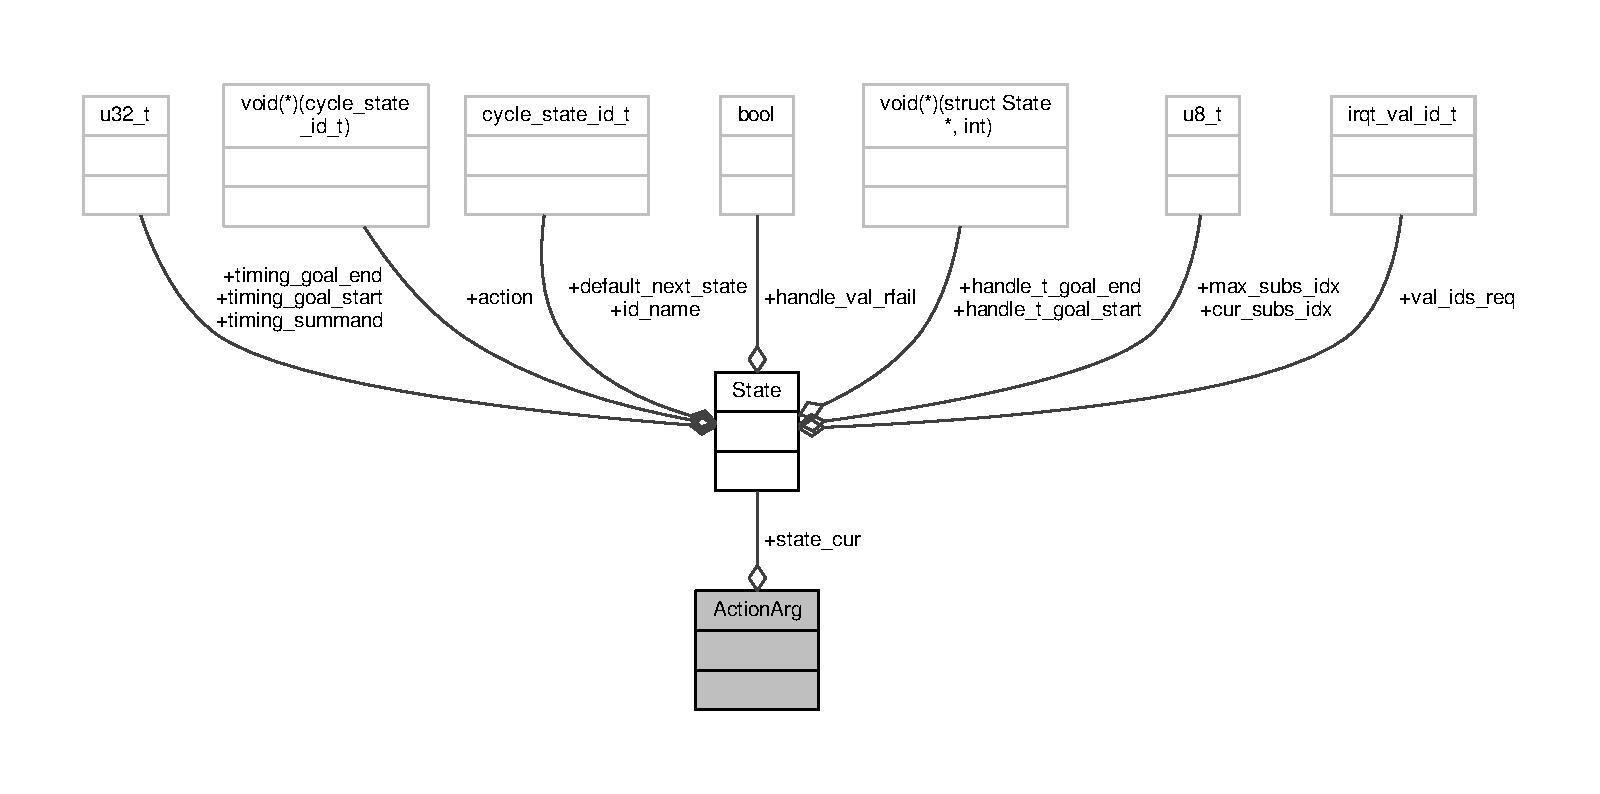
\includegraphics[width=350pt]{struct_action_arg__coll__graph}
\end{center}
\end{figure}
\subsection*{Data Fields}
\begin{DoxyCompactItemize}
\item 
struct \hyperlink{struct_state}{State} $\ast$ \hyperlink{struct_action_arg_a2f7d37145be4a5d1c22f700f31ae2c27}{state\+\_\+cur}
\end{DoxyCompactItemize}


\subsection{Detailed Description}
struct passed to any registered action as argument 

\subsection{Field Documentation}
\index{Action\+Arg@{Action\+Arg}!state\+\_\+cur@{state\+\_\+cur}}
\index{state\+\_\+cur@{state\+\_\+cur}!Action\+Arg@{Action\+Arg}}
\subsubsection[{\texorpdfstring{state\+\_\+cur}{state_cur}}]{\setlength{\rightskip}{0pt plus 5cm}struct {\bf State}$\ast$ state\+\_\+cur}\hypertarget{struct_action_arg_a2f7d37145be4a5d1c22f700f31ae2c27}{}\label{struct_action_arg_a2f7d37145be4a5d1c22f700f31ae2c27}


The documentation for this struct was generated from the following file\+:\begin{DoxyCompactItemize}
\item 
/home/timo/\+Software/zephyr-\/riscv\+\_\+dev/apps/irqperipheral\+\_\+test/src/\hyperlink{states_8h}{states.\+h}\end{DoxyCompactItemize}

\hypertarget{struct_drv_event}{}\section{Drv\+Event Struct Reference}
\label{struct_drv_event}\index{Drv\+Event@{Drv\+Event}}


{\ttfamily \#include $<$irqtestperipheral.\+h$>$}



Collaboration diagram for Drv\+Event\+:\nopagebreak
\begin{figure}[H]
\begin{center}
\leavevmode
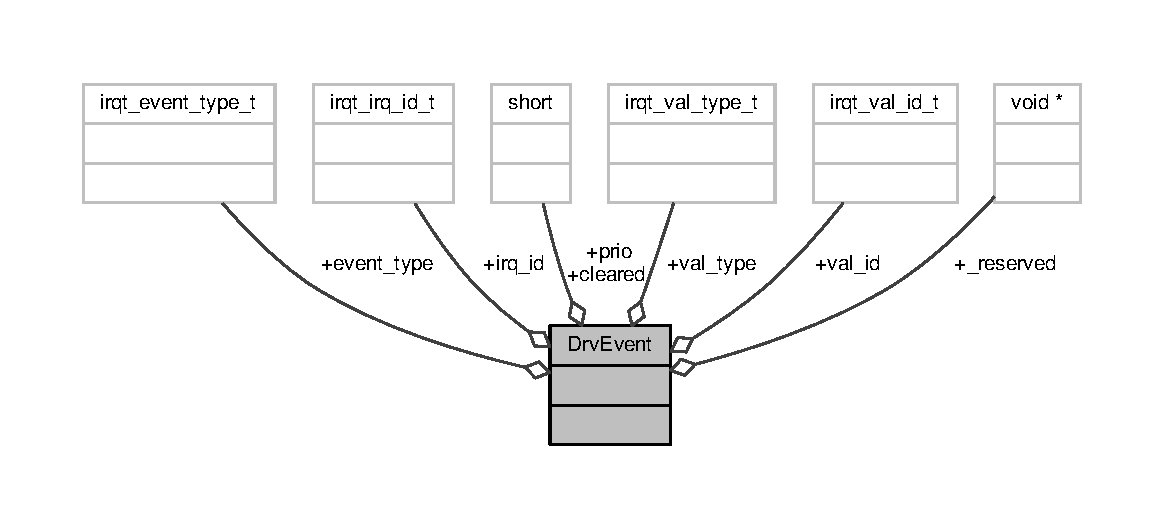
\includegraphics[width=350pt]{struct_drv_event__coll__graph}
\end{center}
\end{figure}
\subsection*{Data Fields}
\begin{DoxyCompactItemize}
\item 
void $\ast$ \hyperlink{struct_drv_event_abb7722001f04208434c040733ffba3c9}{\+\_\+reserved}
\item 
short \hyperlink{struct_drv_event_ac831d1d2fd8bf5bb89ec82259d1930a2}{cleared}
\item 
\hyperlink{irqtestperipheral_8h_a3485d29696b63704b7a6454519c3d0c5}{irqt\+\_\+val\+\_\+id\+\_\+t} \hyperlink{struct_drv_event_aae5ff1cc4fe7007a28ec8c8e7ad7fcad}{val\+\_\+id}
\item 
\hyperlink{irqtestperipheral_8h_a6354e3cbd47a9004937a59f50ede5080}{irqt\+\_\+val\+\_\+type\+\_\+t} \hyperlink{struct_drv_event_a7f525ede95582d630aa5071200d67e74}{val\+\_\+type}
\item 
\hyperlink{irqtestperipheral_8h_a48709c47aad349276bf7506397c044f9}{irqt\+\_\+event\+\_\+type\+\_\+t} \hyperlink{struct_drv_event_a7fb79c00664b2e1634d12eed5b49af7f}{event\+\_\+type}
\item 
\hyperlink{irqtestperipheral_8h_a53f93f474fe7c9fa2072c6e9cea3d6ef}{irqt\+\_\+irq\+\_\+id\+\_\+t} \hyperlink{struct_drv_event_a0b4c8b371cfeb7c552ac3922ac9526ba}{irq\+\_\+id}
\item 
short \hyperlink{struct_drv_event_adcd29556d7e74ba2cb03422da6683017}{prio}
\end{DoxyCompactItemize}


\subsection{Detailed Description}
Driver Event 

\subsection{Field Documentation}
\index{Drv\+Event@{Drv\+Event}!\+\_\+reserved@{\+\_\+reserved}}
\index{\+\_\+reserved@{\+\_\+reserved}!Drv\+Event@{Drv\+Event}}
\subsubsection[{\texorpdfstring{\+\_\+reserved}{_reserved}}]{\setlength{\rightskip}{0pt plus 5cm}void$\ast$ \+\_\+reserved}\hypertarget{struct_drv_event_abb7722001f04208434c040733ffba3c9}{}\label{struct_drv_event_abb7722001f04208434c040733ffba3c9}
\index{Drv\+Event@{Drv\+Event}!cleared@{cleared}}
\index{cleared@{cleared}!Drv\+Event@{Drv\+Event}}
\subsubsection[{\texorpdfstring{cleared}{cleared}}]{\setlength{\rightskip}{0pt plus 5cm}short cleared}\hypertarget{struct_drv_event_ac831d1d2fd8bf5bb89ec82259d1930a2}{}\label{struct_drv_event_ac831d1d2fd8bf5bb89ec82259d1930a2}
\index{Drv\+Event@{Drv\+Event}!event\+\_\+type@{event\+\_\+type}}
\index{event\+\_\+type@{event\+\_\+type}!Drv\+Event@{Drv\+Event}}
\subsubsection[{\texorpdfstring{event\+\_\+type}{event_type}}]{\setlength{\rightskip}{0pt plus 5cm}{\bf irqt\+\_\+event\+\_\+type\+\_\+t} event\+\_\+type}\hypertarget{struct_drv_event_a7fb79c00664b2e1634d12eed5b49af7f}{}\label{struct_drv_event_a7fb79c00664b2e1634d12eed5b49af7f}
\index{Drv\+Event@{Drv\+Event}!irq\+\_\+id@{irq\+\_\+id}}
\index{irq\+\_\+id@{irq\+\_\+id}!Drv\+Event@{Drv\+Event}}
\subsubsection[{\texorpdfstring{irq\+\_\+id}{irq_id}}]{\setlength{\rightskip}{0pt plus 5cm}{\bf irqt\+\_\+irq\+\_\+id\+\_\+t} irq\+\_\+id}\hypertarget{struct_drv_event_a0b4c8b371cfeb7c552ac3922ac9526ba}{}\label{struct_drv_event_a0b4c8b371cfeb7c552ac3922ac9526ba}
\index{Drv\+Event@{Drv\+Event}!prio@{prio}}
\index{prio@{prio}!Drv\+Event@{Drv\+Event}}
\subsubsection[{\texorpdfstring{prio}{prio}}]{\setlength{\rightskip}{0pt plus 5cm}short prio}\hypertarget{struct_drv_event_adcd29556d7e74ba2cb03422da6683017}{}\label{struct_drv_event_adcd29556d7e74ba2cb03422da6683017}
\index{Drv\+Event@{Drv\+Event}!val\+\_\+id@{val\+\_\+id}}
\index{val\+\_\+id@{val\+\_\+id}!Drv\+Event@{Drv\+Event}}
\subsubsection[{\texorpdfstring{val\+\_\+id}{val_id}}]{\setlength{\rightskip}{0pt plus 5cm}{\bf irqt\+\_\+val\+\_\+id\+\_\+t} val\+\_\+id}\hypertarget{struct_drv_event_aae5ff1cc4fe7007a28ec8c8e7ad7fcad}{}\label{struct_drv_event_aae5ff1cc4fe7007a28ec8c8e7ad7fcad}
\index{Drv\+Event@{Drv\+Event}!val\+\_\+type@{val\+\_\+type}}
\index{val\+\_\+type@{val\+\_\+type}!Drv\+Event@{Drv\+Event}}
\subsubsection[{\texorpdfstring{val\+\_\+type}{val_type}}]{\setlength{\rightskip}{0pt plus 5cm}{\bf irqt\+\_\+val\+\_\+type\+\_\+t} val\+\_\+type}\hypertarget{struct_drv_event_a7f525ede95582d630aa5071200d67e74}{}\label{struct_drv_event_a7f525ede95582d630aa5071200d67e74}


The documentation for this struct was generated from the following file\+:\begin{DoxyCompactItemize}
\item 
/home/timo/\+Software/zephyr-\/riscv\+\_\+dev/apps/irqperipheral\+\_\+test/src/drivers/irqtestperipheral/src/\hyperlink{irqtestperipheral_8h}{irqtestperipheral.\+h}\end{DoxyCompactItemize}

\hypertarget{struct_drv_value__bool}{}\section{Drv\+Value\+\_\+bool Struct Reference}
\label{struct_drv_value__bool}\index{Drv\+Value\+\_\+bool@{Drv\+Value\+\_\+bool}}


{\ttfamily \#include $<$irqtestperipheral.\+h$>$}



Collaboration diagram for Drv\+Value\+\_\+bool\+:\nopagebreak
\begin{figure}[H]
\begin{center}
\leavevmode
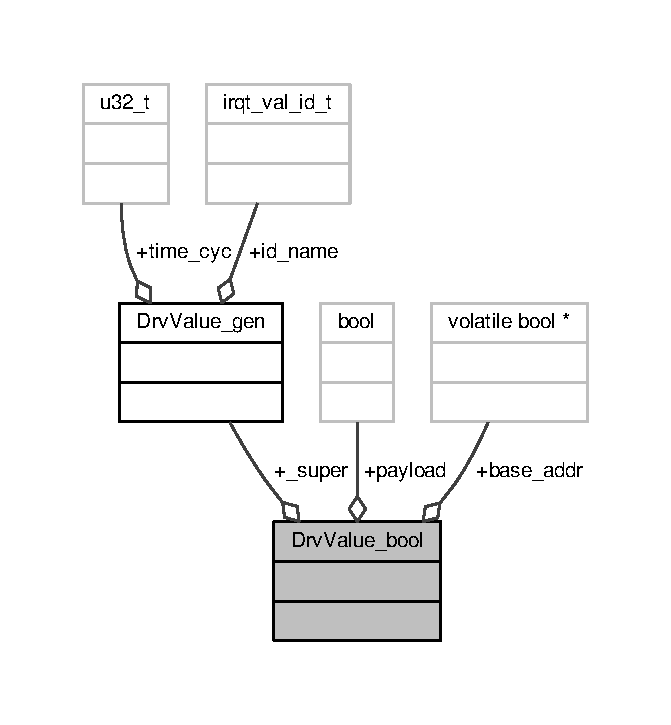
\includegraphics[width=322pt]{struct_drv_value__bool__coll__graph}
\end{center}
\end{figure}
\subsection*{Data Fields}
\begin{DoxyCompactItemize}
\item 
struct \hyperlink{struct_drv_value__gen}{Drv\+Value\+\_\+gen} \hyperlink{struct_drv_value__bool_ad6a22febddaa20faa4af2f9fed5766f0}{\+\_\+super}
\item 
volatile bool $\ast$ \hyperlink{struct_drv_value__bool_af9a44b0b9251fbefd04c475aaab792ad}{base\+\_\+addr}
\item 
bool \hyperlink{struct_drv_value__bool_abdbaaae567d94da3de1d6aa546b501ac}{payload}
\end{DoxyCompactItemize}


\subsection{Field Documentation}
\index{Drv\+Value\+\_\+bool@{Drv\+Value\+\_\+bool}!\+\_\+super@{\+\_\+super}}
\index{\+\_\+super@{\+\_\+super}!Drv\+Value\+\_\+bool@{Drv\+Value\+\_\+bool}}
\subsubsection[{\texorpdfstring{\+\_\+super}{_super}}]{\setlength{\rightskip}{0pt plus 5cm}struct {\bf Drv\+Value\+\_\+gen} \+\_\+super}\hypertarget{struct_drv_value__bool_ad6a22febddaa20faa4af2f9fed5766f0}{}\label{struct_drv_value__bool_ad6a22febddaa20faa4af2f9fed5766f0}
\index{Drv\+Value\+\_\+bool@{Drv\+Value\+\_\+bool}!base\+\_\+addr@{base\+\_\+addr}}
\index{base\+\_\+addr@{base\+\_\+addr}!Drv\+Value\+\_\+bool@{Drv\+Value\+\_\+bool}}
\subsubsection[{\texorpdfstring{base\+\_\+addr}{base_addr}}]{\setlength{\rightskip}{0pt plus 5cm}volatile bool$\ast$ base\+\_\+addr}\hypertarget{struct_drv_value__bool_af9a44b0b9251fbefd04c475aaab792ad}{}\label{struct_drv_value__bool_af9a44b0b9251fbefd04c475aaab792ad}
\index{Drv\+Value\+\_\+bool@{Drv\+Value\+\_\+bool}!payload@{payload}}
\index{payload@{payload}!Drv\+Value\+\_\+bool@{Drv\+Value\+\_\+bool}}
\subsubsection[{\texorpdfstring{payload}{payload}}]{\setlength{\rightskip}{0pt plus 5cm}bool payload}\hypertarget{struct_drv_value__bool_abdbaaae567d94da3de1d6aa546b501ac}{}\label{struct_drv_value__bool_abdbaaae567d94da3de1d6aa546b501ac}


The documentation for this struct was generated from the following file\+:\begin{DoxyCompactItemize}
\item 
/home/timo/\+Software/zephyr-\/riscv\+\_\+dev/apps/irqperipheral\+\_\+test/src/drivers/irqtestperipheral/src/\hyperlink{irqtestperipheral_8h}{irqtestperipheral.\+h}\end{DoxyCompactItemize}

\hypertarget{struct_drv_value__gen}{}\section{Drv\+Value\+\_\+gen Struct Reference}
\label{struct_drv_value__gen}\index{Drv\+Value\+\_\+gen@{Drv\+Value\+\_\+gen}}


{\ttfamily \#include $<$irqtestperipheral.\+h$>$}



Collaboration diagram for Drv\+Value\+\_\+gen\+:\nopagebreak
\begin{figure}[H]
\begin{center}
\leavevmode
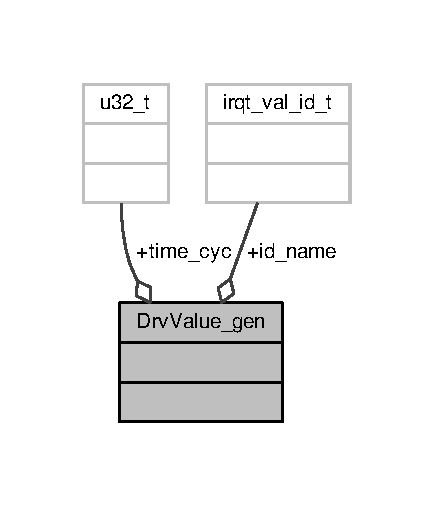
\includegraphics[width=208pt]{struct_drv_value__gen__coll__graph}
\end{center}
\end{figure}
\subsection*{Data Fields}
\begin{DoxyCompactItemize}
\item 
\hyperlink{irqtestperipheral_8h_a3485d29696b63704b7a6454519c3d0c5}{irqt\+\_\+val\+\_\+id\+\_\+t} \hyperlink{struct_drv_value__gen_a5226c1d3c4b403e66022cb0a73132166}{id\+\_\+name}
\item 
u32\+\_\+t \hyperlink{struct_drv_value__gen_a916ebe230253097fafdb1a2d73b1a44d}{time\+\_\+cyc}
\end{DoxyCompactItemize}


\subsection{Detailed Description}
Driver Value. Generic parent struct to be casted to correct subtype. This can be inferred by .val\+\_\+type in a \hyperlink{struct_drv_event}{Drv\+Event}. 

\subsection{Field Documentation}
\index{Drv\+Value\+\_\+gen@{Drv\+Value\+\_\+gen}!id\+\_\+name@{id\+\_\+name}}
\index{id\+\_\+name@{id\+\_\+name}!Drv\+Value\+\_\+gen@{Drv\+Value\+\_\+gen}}
\subsubsection[{\texorpdfstring{id\+\_\+name}{id_name}}]{\setlength{\rightskip}{0pt plus 5cm}{\bf irqt\+\_\+val\+\_\+id\+\_\+t} id\+\_\+name}\hypertarget{struct_drv_value__gen_a5226c1d3c4b403e66022cb0a73132166}{}\label{struct_drv_value__gen_a5226c1d3c4b403e66022cb0a73132166}
\index{Drv\+Value\+\_\+gen@{Drv\+Value\+\_\+gen}!time\+\_\+cyc@{time\+\_\+cyc}}
\index{time\+\_\+cyc@{time\+\_\+cyc}!Drv\+Value\+\_\+gen@{Drv\+Value\+\_\+gen}}
\subsubsection[{\texorpdfstring{time\+\_\+cyc}{time_cyc}}]{\setlength{\rightskip}{0pt plus 5cm}u32\+\_\+t time\+\_\+cyc}\hypertarget{struct_drv_value__gen_a916ebe230253097fafdb1a2d73b1a44d}{}\label{struct_drv_value__gen_a916ebe230253097fafdb1a2d73b1a44d}


The documentation for this struct was generated from the following file\+:\begin{DoxyCompactItemize}
\item 
/home/timo/\+Software/zephyr-\/riscv\+\_\+dev/apps/irqperipheral\+\_\+test/src/drivers/irqtestperipheral/src/\hyperlink{irqtestperipheral_8h}{irqtestperipheral.\+h}\end{DoxyCompactItemize}

\hypertarget{struct_drv_value__int}{}\section{Drv\+Value\+\_\+int Struct Reference}
\label{struct_drv_value__int}\index{Drv\+Value\+\_\+int@{Drv\+Value\+\_\+int}}


{\ttfamily \#include $<$irqtestperipheral.\+h$>$}



Collaboration diagram for Drv\+Value\+\_\+int\+:\nopagebreak
\begin{figure}[H]
\begin{center}
\leavevmode
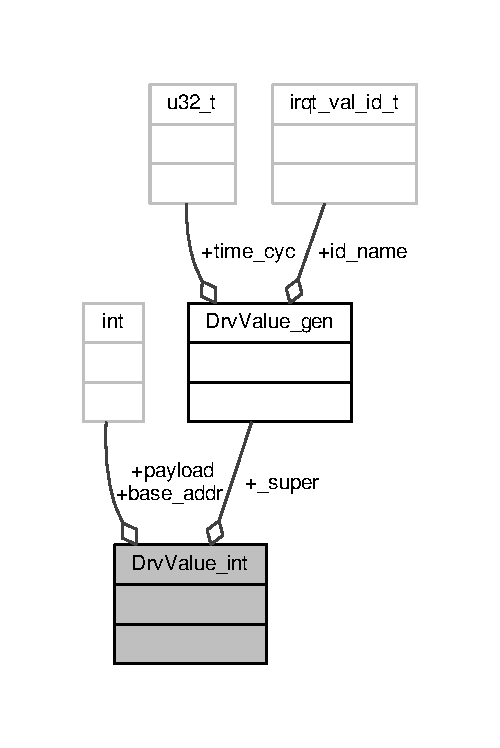
\includegraphics[width=240pt]{struct_drv_value__int__coll__graph}
\end{center}
\end{figure}
\subsection*{Data Fields}
\begin{DoxyCompactItemize}
\item 
struct \hyperlink{struct_drv_value__gen}{Drv\+Value\+\_\+gen} \hyperlink{struct_drv_value__int_ad6a22febddaa20faa4af2f9fed5766f0}{\+\_\+super}
\item 
volatile int $\ast$ \hyperlink{struct_drv_value__int_ae2918bea8bf855b64182bd166cb8966d}{base\+\_\+addr}
\item 
int \hyperlink{struct_drv_value__int_a86d3b28b783f5b0e9cf208f0461a6f0b}{payload}
\end{DoxyCompactItemize}


\subsection{Field Documentation}
\index{Drv\+Value\+\_\+int@{Drv\+Value\+\_\+int}!\+\_\+super@{\+\_\+super}}
\index{\+\_\+super@{\+\_\+super}!Drv\+Value\+\_\+int@{Drv\+Value\+\_\+int}}
\subsubsection[{\texorpdfstring{\+\_\+super}{_super}}]{\setlength{\rightskip}{0pt plus 5cm}struct {\bf Drv\+Value\+\_\+gen} \+\_\+super}\hypertarget{struct_drv_value__int_ad6a22febddaa20faa4af2f9fed5766f0}{}\label{struct_drv_value__int_ad6a22febddaa20faa4af2f9fed5766f0}
\index{Drv\+Value\+\_\+int@{Drv\+Value\+\_\+int}!base\+\_\+addr@{base\+\_\+addr}}
\index{base\+\_\+addr@{base\+\_\+addr}!Drv\+Value\+\_\+int@{Drv\+Value\+\_\+int}}
\subsubsection[{\texorpdfstring{base\+\_\+addr}{base_addr}}]{\setlength{\rightskip}{0pt plus 5cm}volatile int$\ast$ base\+\_\+addr}\hypertarget{struct_drv_value__int_ae2918bea8bf855b64182bd166cb8966d}{}\label{struct_drv_value__int_ae2918bea8bf855b64182bd166cb8966d}
\index{Drv\+Value\+\_\+int@{Drv\+Value\+\_\+int}!payload@{payload}}
\index{payload@{payload}!Drv\+Value\+\_\+int@{Drv\+Value\+\_\+int}}
\subsubsection[{\texorpdfstring{payload}{payload}}]{\setlength{\rightskip}{0pt plus 5cm}int payload}\hypertarget{struct_drv_value__int_a86d3b28b783f5b0e9cf208f0461a6f0b}{}\label{struct_drv_value__int_a86d3b28b783f5b0e9cf208f0461a6f0b}


The documentation for this struct was generated from the following file\+:\begin{DoxyCompactItemize}
\item 
/home/timo/\+Software/zephyr-\/riscv\+\_\+dev/apps/irqperipheral\+\_\+test/src/drivers/irqtestperipheral/src/\hyperlink{irqtestperipheral_8h}{irqtestperipheral.\+h}\end{DoxyCompactItemize}

\hypertarget{struct_drv_value__uint}{}\section{Drv\+Value\+\_\+uint Struct Reference}
\label{struct_drv_value__uint}\index{Drv\+Value\+\_\+uint@{Drv\+Value\+\_\+uint}}


{\ttfamily \#include $<$irqtestperipheral.\+h$>$}



Collaboration diagram for Drv\+Value\+\_\+uint\+:\nopagebreak
\begin{figure}[H]
\begin{center}
\leavevmode
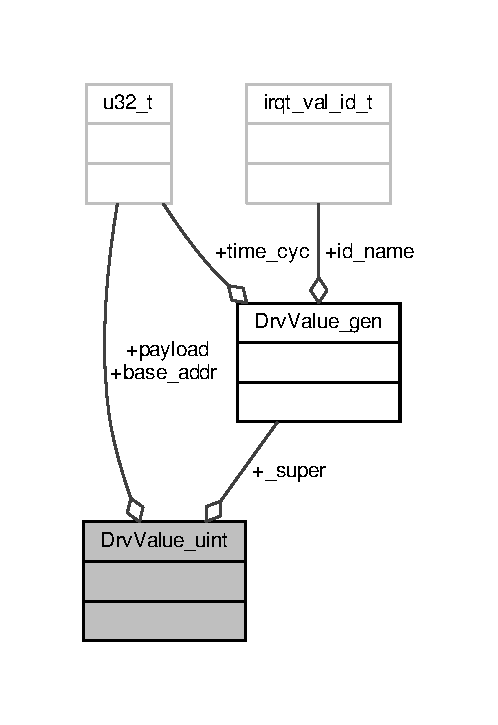
\includegraphics[width=239pt]{struct_drv_value__uint__coll__graph}
\end{center}
\end{figure}
\subsection*{Data Fields}
\begin{DoxyCompactItemize}
\item 
struct \hyperlink{struct_drv_value__gen}{Drv\+Value\+\_\+gen} \hyperlink{struct_drv_value__uint_ad6a22febddaa20faa4af2f9fed5766f0}{\+\_\+super}
\item 
volatile u32\+\_\+t $\ast$ \hyperlink{struct_drv_value__uint_af745320979cc5b64a90dda3de0bb6f9a}{base\+\_\+addr}
\item 
u32\+\_\+t \hyperlink{struct_drv_value__uint_a162d02c866faff1801fd317ce7edfdd7}{payload}
\end{DoxyCompactItemize}


\subsection{Field Documentation}
\index{Drv\+Value\+\_\+uint@{Drv\+Value\+\_\+uint}!\+\_\+super@{\+\_\+super}}
\index{\+\_\+super@{\+\_\+super}!Drv\+Value\+\_\+uint@{Drv\+Value\+\_\+uint}}
\subsubsection[{\texorpdfstring{\+\_\+super}{_super}}]{\setlength{\rightskip}{0pt plus 5cm}struct {\bf Drv\+Value\+\_\+gen} \+\_\+super}\hypertarget{struct_drv_value__uint_ad6a22febddaa20faa4af2f9fed5766f0}{}\label{struct_drv_value__uint_ad6a22febddaa20faa4af2f9fed5766f0}
\index{Drv\+Value\+\_\+uint@{Drv\+Value\+\_\+uint}!base\+\_\+addr@{base\+\_\+addr}}
\index{base\+\_\+addr@{base\+\_\+addr}!Drv\+Value\+\_\+uint@{Drv\+Value\+\_\+uint}}
\subsubsection[{\texorpdfstring{base\+\_\+addr}{base_addr}}]{\setlength{\rightskip}{0pt plus 5cm}volatile u32\+\_\+t$\ast$ base\+\_\+addr}\hypertarget{struct_drv_value__uint_af745320979cc5b64a90dda3de0bb6f9a}{}\label{struct_drv_value__uint_af745320979cc5b64a90dda3de0bb6f9a}
\index{Drv\+Value\+\_\+uint@{Drv\+Value\+\_\+uint}!payload@{payload}}
\index{payload@{payload}!Drv\+Value\+\_\+uint@{Drv\+Value\+\_\+uint}}
\subsubsection[{\texorpdfstring{payload}{payload}}]{\setlength{\rightskip}{0pt plus 5cm}u32\+\_\+t payload}\hypertarget{struct_drv_value__uint_a162d02c866faff1801fd317ce7edfdd7}{}\label{struct_drv_value__uint_a162d02c866faff1801fd317ce7edfdd7}


The documentation for this struct was generated from the following file\+:\begin{DoxyCompactItemize}
\item 
/home/timo/\+Software/zephyr-\/riscv\+\_\+dev/apps/irqperipheral\+\_\+test/src/drivers/irqtestperipheral/src/\hyperlink{irqtestperipheral_8h}{irqtestperipheral.\+h}\end{DoxyCompactItemize}

\hypertarget{struct_perf___event}{}\section{Perf\+\_\+\+Event Struct Reference}
\label{struct_perf___event}\index{Perf\+\_\+\+Event@{Perf\+\_\+\+Event}}


{\ttfamily \#include $<$state\+\_\+manager.\+h$>$}



Collaboration diagram for Perf\+\_\+\+Event\+:\nopagebreak
\begin{figure}[H]
\begin{center}
\leavevmode
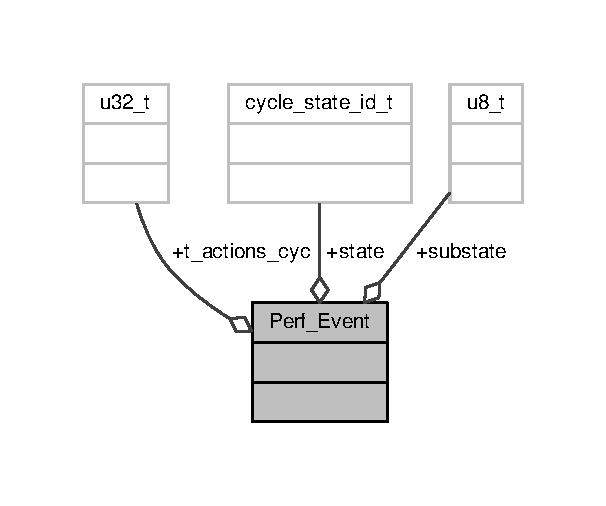
\includegraphics[width=291pt]{struct_perf___event__coll__graph}
\end{center}
\end{figure}
\subsection*{Data Fields}
\begin{DoxyCompactItemize}
\item 
\hyperlink{states_8h_a9e0ef0bc98a491d55216d9485e562252}{cycle\+\_\+state\+\_\+id\+\_\+t} \hyperlink{struct_perf___event_a6ed5d93e163f36fafba6a6fa602ab3f0}{state}
\item 
u8\+\_\+t \hyperlink{struct_perf___event_aa719d2e676dc0eeaafeaae9bbc1849f0}{substate}
\item 
u32\+\_\+t \hyperlink{struct_perf___event_a19240b276493b0f29eb1495b8b03a644}{t\+\_\+actions\+\_\+cyc}
\end{DoxyCompactItemize}


\subsection{Detailed Description}
used easuring performance of actions (Can use switch events, too.) 

\subsection{Field Documentation}
\index{Perf\+\_\+\+Event@{Perf\+\_\+\+Event}!state@{state}}
\index{state@{state}!Perf\+\_\+\+Event@{Perf\+\_\+\+Event}}
\subsubsection[{\texorpdfstring{state}{state}}]{\setlength{\rightskip}{0pt plus 5cm}{\bf cycle\+\_\+state\+\_\+id\+\_\+t} state}\hypertarget{struct_perf___event_a6ed5d93e163f36fafba6a6fa602ab3f0}{}\label{struct_perf___event_a6ed5d93e163f36fafba6a6fa602ab3f0}
\index{Perf\+\_\+\+Event@{Perf\+\_\+\+Event}!substate@{substate}}
\index{substate@{substate}!Perf\+\_\+\+Event@{Perf\+\_\+\+Event}}
\subsubsection[{\texorpdfstring{substate}{substate}}]{\setlength{\rightskip}{0pt plus 5cm}u8\+\_\+t substate}\hypertarget{struct_perf___event_aa719d2e676dc0eeaafeaae9bbc1849f0}{}\label{struct_perf___event_aa719d2e676dc0eeaafeaae9bbc1849f0}
\index{Perf\+\_\+\+Event@{Perf\+\_\+\+Event}!t\+\_\+actions\+\_\+cyc@{t\+\_\+actions\+\_\+cyc}}
\index{t\+\_\+actions\+\_\+cyc@{t\+\_\+actions\+\_\+cyc}!Perf\+\_\+\+Event@{Perf\+\_\+\+Event}}
\subsubsection[{\texorpdfstring{t\+\_\+actions\+\_\+cyc}{t_actions_cyc}}]{\setlength{\rightskip}{0pt plus 5cm}u32\+\_\+t t\+\_\+actions\+\_\+cyc}\hypertarget{struct_perf___event_a19240b276493b0f29eb1495b8b03a644}{}\label{struct_perf___event_a19240b276493b0f29eb1495b8b03a644}


The documentation for this struct was generated from the following file\+:\begin{DoxyCompactItemize}
\item 
/home/timo/\+Software/zephyr-\/riscv\+\_\+dev/apps/irqperipheral\+\_\+test/src/\hyperlink{state__manager_8h}{state\+\_\+manager.\+h}\end{DoxyCompactItemize}

\hypertarget{struct_s_m_event}{}\section{S\+M\+Event Struct Reference}
\label{struct_s_m_event}\index{S\+M\+Event@{S\+M\+Event}}


Controls switching of state\+\_\+manager states.  




Collaboration diagram for S\+M\+Event\+:\nopagebreak
\begin{figure}[H]
\begin{center}
\leavevmode
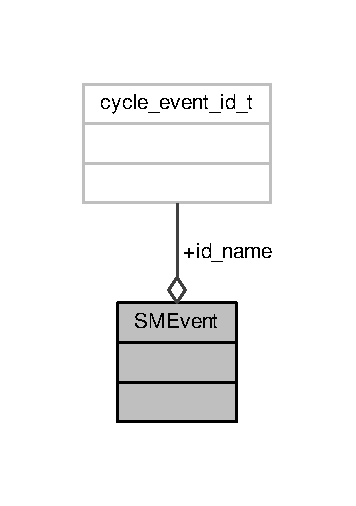
\includegraphics[width=171pt]{struct_s_m_event__coll__graph}
\end{center}
\end{figure}
\subsection*{Data Fields}
\begin{DoxyCompactItemize}
\item 
\hyperlink{states_8h_a1956f5c4955f21ca67d43209bc162438}{cycle\+\_\+event\+\_\+id\+\_\+t} \hyperlink{struct_s_m_event_a20f4c1f646da07c42e0e23c9f5dc5c30}{id\+\_\+name}
\end{DoxyCompactItemize}


\subsection{Detailed Description}
Controls switching of state\+\_\+manager states. 

\subsection{Field Documentation}
\index{S\+M\+Event@{S\+M\+Event}!id\+\_\+name@{id\+\_\+name}}
\index{id\+\_\+name@{id\+\_\+name}!S\+M\+Event@{S\+M\+Event}}
\subsubsection[{\texorpdfstring{id\+\_\+name}{id_name}}]{\setlength{\rightskip}{0pt plus 5cm}{\bf cycle\+\_\+event\+\_\+id\+\_\+t} id\+\_\+name}\hypertarget{struct_s_m_event_a20f4c1f646da07c42e0e23c9f5dc5c30}{}\label{struct_s_m_event_a20f4c1f646da07c42e0e23c9f5dc5c30}


The documentation for this struct was generated from the following file\+:\begin{DoxyCompactItemize}
\item 
/home/timo/\+Software/zephyr-\/riscv\+\_\+dev/apps/irqperipheral\+\_\+test/src/\hyperlink{state__manager_8c}{state\+\_\+manager.\+c}\end{DoxyCompactItemize}

\hypertarget{struct_state}{}\section{State Struct Reference}
\label{struct_state}\index{State@{State}}


{\ttfamily \#include $<$states.\+h$>$}



Collaboration diagram for State\+:\nopagebreak
\begin{figure}[H]
\begin{center}
\leavevmode
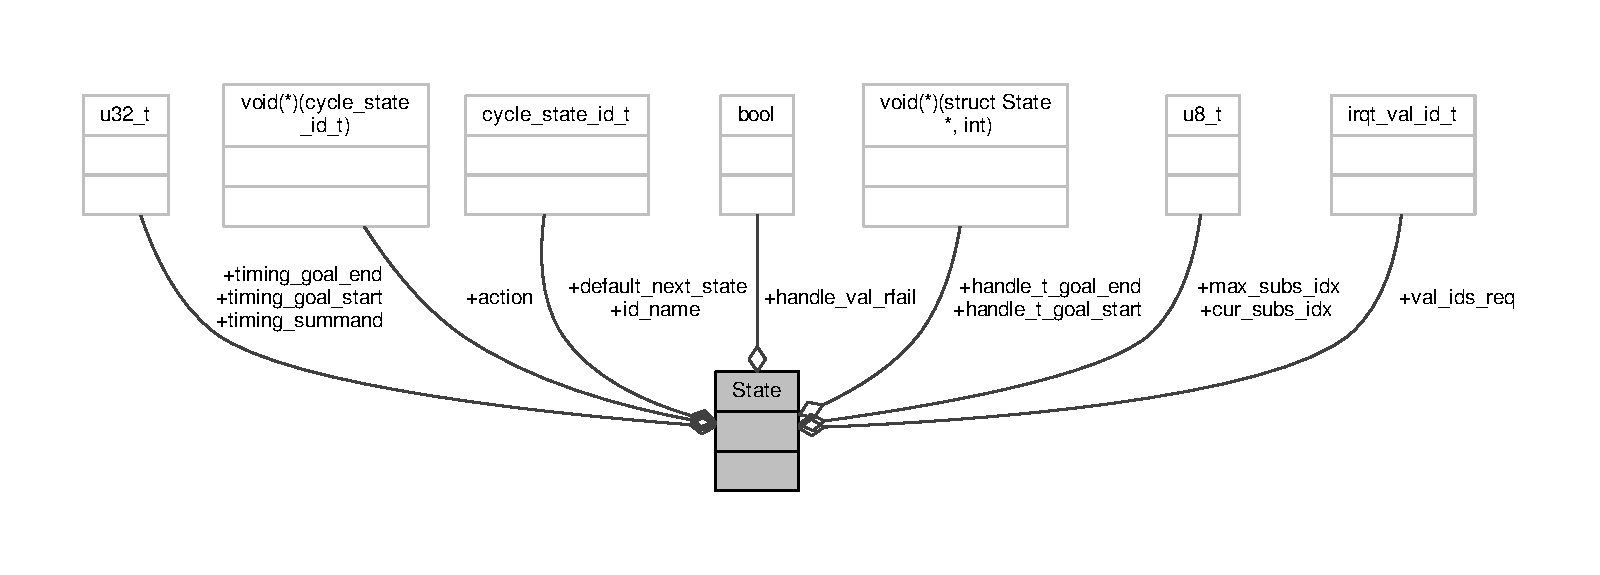
\includegraphics[width=350pt]{struct_state__coll__graph}
\end{center}
\end{figure}
\subsection*{Data Fields}
\begin{DoxyCompactItemize}
\item 
\hyperlink{states_8h_a9e0ef0bc98a491d55216d9485e562252}{cycle\+\_\+state\+\_\+id\+\_\+t} \hyperlink{struct_state_abb59b67712b25f52806b3a75d5ced8e1}{id\+\_\+name}
\item 
\hyperlink{states_8h_a9e0ef0bc98a491d55216d9485e562252}{cycle\+\_\+state\+\_\+id\+\_\+t} \hyperlink{struct_state_af9d8ee1d5b2527603692e4e16a510dfc}{default\+\_\+next\+\_\+state}
\item 
u32\+\_\+t \hyperlink{struct_state_a460c2961861ad0bfe6b175e2d310fa5a}{timing\+\_\+goal\+\_\+start}
\item 
u32\+\_\+t \hyperlink{struct_state_af1c6f6dee4c21d85ddf7da3864d1cbee}{timing\+\_\+goal\+\_\+end}
\item 
\hyperlink{irqtestperipheral_8h_a3485d29696b63704b7a6454519c3d0c5}{irqt\+\_\+val\+\_\+id\+\_\+t} \hyperlink{struct_state_ab6d93aa56200181dd2b06e3eda4bc090}{val\+\_\+ids\+\_\+req} \mbox{[}\hyperlink{states_8h_ac7f2a6758dc88e00b49c5d4152ef468e}{S\+T\+A\+T\+E\+S\+\_\+\+R\+E\+Q\+\_\+\+V\+A\+L\+S\+\_\+\+M\+AX}\mbox{]}
\item 
void($\ast$ \hyperlink{struct_state_a55d5000db1bebc1ee6f6d6d5b3bb6673}{action} )(\hyperlink{states_8h_a9e0ef0bc98a491d55216d9485e562252}{cycle\+\_\+state\+\_\+id\+\_\+t})
\item 
void($\ast$ \hyperlink{struct_state_a85025dd68c4035546894c6b14542e528}{handle\+\_\+t\+\_\+goal\+\_\+start} )(struct \hyperlink{struct_state}{State} $\ast$, int)
\item 
void($\ast$ \hyperlink{struct_state_ab347ebabf77bbde522554a8d663ec4a5}{handle\+\_\+t\+\_\+goal\+\_\+end} )(struct \hyperlink{struct_state}{State} $\ast$, int)
\item 
bool($\ast$ \hyperlink{struct_state_a840b9de3ab0a84eed21af071a716348b}{handle\+\_\+val\+\_\+rfail} )(struct \hyperlink{struct_state}{State} $\ast$)
\item 
u8\+\_\+t \hyperlink{struct_state_a06b41367cc51f722ce294c92dc341e93}{cur\+\_\+subs\+\_\+idx}
\item 
u8\+\_\+t \hyperlink{struct_state_a73f7b81a54eb23206152bb815a0de136}{max\+\_\+subs\+\_\+idx}
\item 
u32\+\_\+t \hyperlink{struct_state_ad775f6c08e398dddae5d7fbcd8487b6d}{timing\+\_\+summand}
\end{DoxyCompactItemize}


\subsection{Field Documentation}
\index{State@{State}!action@{action}}
\index{action@{action}!State@{State}}
\subsubsection[{\texorpdfstring{action}{action}}]{\setlength{\rightskip}{0pt plus 5cm}void($\ast$ action) ({\bf cycle\+\_\+state\+\_\+id\+\_\+t})}\hypertarget{struct_state_a55d5000db1bebc1ee6f6d6d5b3bb6673}{}\label{struct_state_a55d5000db1bebc1ee6f6d6d5b3bb6673}
\index{State@{State}!cur\+\_\+subs\+\_\+idx@{cur\+\_\+subs\+\_\+idx}}
\index{cur\+\_\+subs\+\_\+idx@{cur\+\_\+subs\+\_\+idx}!State@{State}}
\subsubsection[{\texorpdfstring{cur\+\_\+subs\+\_\+idx}{cur_subs_idx}}]{\setlength{\rightskip}{0pt plus 5cm}u8\+\_\+t cur\+\_\+subs\+\_\+idx}\hypertarget{struct_state_a06b41367cc51f722ce294c92dc341e93}{}\label{struct_state_a06b41367cc51f722ce294c92dc341e93}
\index{State@{State}!default\+\_\+next\+\_\+state@{default\+\_\+next\+\_\+state}}
\index{default\+\_\+next\+\_\+state@{default\+\_\+next\+\_\+state}!State@{State}}
\subsubsection[{\texorpdfstring{default\+\_\+next\+\_\+state}{default_next_state}}]{\setlength{\rightskip}{0pt plus 5cm}{\bf cycle\+\_\+state\+\_\+id\+\_\+t} default\+\_\+next\+\_\+state}\hypertarget{struct_state_af9d8ee1d5b2527603692e4e16a510dfc}{}\label{struct_state_af9d8ee1d5b2527603692e4e16a510dfc}
\index{State@{State}!handle\+\_\+t\+\_\+goal\+\_\+end@{handle\+\_\+t\+\_\+goal\+\_\+end}}
\index{handle\+\_\+t\+\_\+goal\+\_\+end@{handle\+\_\+t\+\_\+goal\+\_\+end}!State@{State}}
\subsubsection[{\texorpdfstring{handle\+\_\+t\+\_\+goal\+\_\+end}{handle_t_goal_end}}]{\setlength{\rightskip}{0pt plus 5cm}void($\ast$ handle\+\_\+t\+\_\+goal\+\_\+end) (struct {\bf State} $\ast$, int)}\hypertarget{struct_state_ab347ebabf77bbde522554a8d663ec4a5}{}\label{struct_state_ab347ebabf77bbde522554a8d663ec4a5}
\index{State@{State}!handle\+\_\+t\+\_\+goal\+\_\+start@{handle\+\_\+t\+\_\+goal\+\_\+start}}
\index{handle\+\_\+t\+\_\+goal\+\_\+start@{handle\+\_\+t\+\_\+goal\+\_\+start}!State@{State}}
\subsubsection[{\texorpdfstring{handle\+\_\+t\+\_\+goal\+\_\+start}{handle_t_goal_start}}]{\setlength{\rightskip}{0pt plus 5cm}void($\ast$ handle\+\_\+t\+\_\+goal\+\_\+start) (struct {\bf State} $\ast$, int)}\hypertarget{struct_state_a85025dd68c4035546894c6b14542e528}{}\label{struct_state_a85025dd68c4035546894c6b14542e528}
\index{State@{State}!handle\+\_\+val\+\_\+rfail@{handle\+\_\+val\+\_\+rfail}}
\index{handle\+\_\+val\+\_\+rfail@{handle\+\_\+val\+\_\+rfail}!State@{State}}
\subsubsection[{\texorpdfstring{handle\+\_\+val\+\_\+rfail}{handle_val_rfail}}]{\setlength{\rightskip}{0pt plus 5cm}bool($\ast$ handle\+\_\+val\+\_\+rfail) (struct {\bf State} $\ast$)}\hypertarget{struct_state_a840b9de3ab0a84eed21af071a716348b}{}\label{struct_state_a840b9de3ab0a84eed21af071a716348b}
\index{State@{State}!id\+\_\+name@{id\+\_\+name}}
\index{id\+\_\+name@{id\+\_\+name}!State@{State}}
\subsubsection[{\texorpdfstring{id\+\_\+name}{id_name}}]{\setlength{\rightskip}{0pt plus 5cm}{\bf cycle\+\_\+state\+\_\+id\+\_\+t} id\+\_\+name}\hypertarget{struct_state_abb59b67712b25f52806b3a75d5ced8e1}{}\label{struct_state_abb59b67712b25f52806b3a75d5ced8e1}
\index{State@{State}!max\+\_\+subs\+\_\+idx@{max\+\_\+subs\+\_\+idx}}
\index{max\+\_\+subs\+\_\+idx@{max\+\_\+subs\+\_\+idx}!State@{State}}
\subsubsection[{\texorpdfstring{max\+\_\+subs\+\_\+idx}{max_subs_idx}}]{\setlength{\rightskip}{0pt plus 5cm}u8\+\_\+t max\+\_\+subs\+\_\+idx}\hypertarget{struct_state_a73f7b81a54eb23206152bb815a0de136}{}\label{struct_state_a73f7b81a54eb23206152bb815a0de136}
\index{State@{State}!timing\+\_\+goal\+\_\+end@{timing\+\_\+goal\+\_\+end}}
\index{timing\+\_\+goal\+\_\+end@{timing\+\_\+goal\+\_\+end}!State@{State}}
\subsubsection[{\texorpdfstring{timing\+\_\+goal\+\_\+end}{timing_goal_end}}]{\setlength{\rightskip}{0pt plus 5cm}u32\+\_\+t timing\+\_\+goal\+\_\+end}\hypertarget{struct_state_af1c6f6dee4c21d85ddf7da3864d1cbee}{}\label{struct_state_af1c6f6dee4c21d85ddf7da3864d1cbee}
\index{State@{State}!timing\+\_\+goal\+\_\+start@{timing\+\_\+goal\+\_\+start}}
\index{timing\+\_\+goal\+\_\+start@{timing\+\_\+goal\+\_\+start}!State@{State}}
\subsubsection[{\texorpdfstring{timing\+\_\+goal\+\_\+start}{timing_goal_start}}]{\setlength{\rightskip}{0pt plus 5cm}u32\+\_\+t timing\+\_\+goal\+\_\+start}\hypertarget{struct_state_a460c2961861ad0bfe6b175e2d310fa5a}{}\label{struct_state_a460c2961861ad0bfe6b175e2d310fa5a}
\index{State@{State}!timing\+\_\+summand@{timing\+\_\+summand}}
\index{timing\+\_\+summand@{timing\+\_\+summand}!State@{State}}
\subsubsection[{\texorpdfstring{timing\+\_\+summand}{timing_summand}}]{\setlength{\rightskip}{0pt plus 5cm}u32\+\_\+t timing\+\_\+summand}\hypertarget{struct_state_ad775f6c08e398dddae5d7fbcd8487b6d}{}\label{struct_state_ad775f6c08e398dddae5d7fbcd8487b6d}
\index{State@{State}!val\+\_\+ids\+\_\+req@{val\+\_\+ids\+\_\+req}}
\index{val\+\_\+ids\+\_\+req@{val\+\_\+ids\+\_\+req}!State@{State}}
\subsubsection[{\texorpdfstring{val\+\_\+ids\+\_\+req}{val_ids_req}}]{\setlength{\rightskip}{0pt plus 5cm}{\bf irqt\+\_\+val\+\_\+id\+\_\+t} val\+\_\+ids\+\_\+req\mbox{[}{\bf S\+T\+A\+T\+E\+S\+\_\+\+R\+E\+Q\+\_\+\+V\+A\+L\+S\+\_\+\+M\+AX}\mbox{]}}\hypertarget{struct_state_ab6d93aa56200181dd2b06e3eda4bc090}{}\label{struct_state_ab6d93aa56200181dd2b06e3eda4bc090}


The documentation for this struct was generated from the following file\+:\begin{DoxyCompactItemize}
\item 
/home/timo/\+Software/zephyr-\/riscv\+\_\+dev/apps/irqperipheral\+\_\+test/src/\hyperlink{states_8h}{states.\+h}\end{DoxyCompactItemize}

\hypertarget{struct_switch___event}{}\section{Switch\+\_\+\+Event Struct Reference}
\label{struct_switch___event}\index{Switch\+\_\+\+Event@{Switch\+\_\+\+Event}}


used for logging  




{\ttfamily \#include $<$state\+\_\+manager.\+h$>$}



Collaboration diagram for Switch\+\_\+\+Event\+:\nopagebreak
\begin{figure}[H]
\begin{center}
\leavevmode
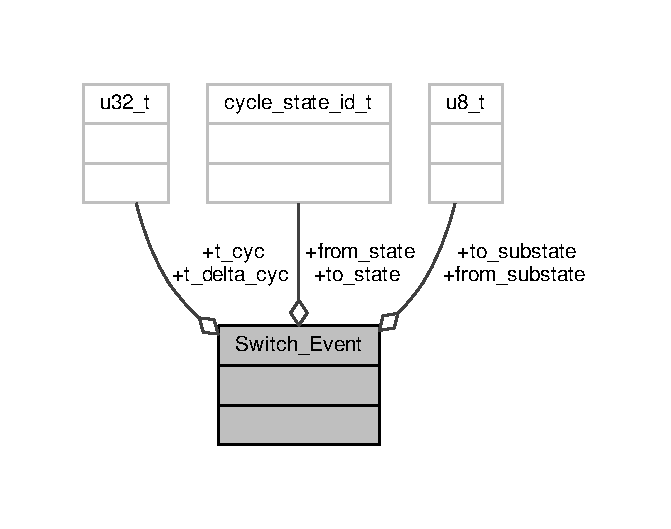
\includegraphics[width=322pt]{struct_switch___event__coll__graph}
\end{center}
\end{figure}
\subsection*{Data Fields}
\begin{DoxyCompactItemize}
\item 
\hyperlink{states_8h_a9e0ef0bc98a491d55216d9485e562252}{cycle\+\_\+state\+\_\+id\+\_\+t} \hyperlink{struct_switch___event_ace1ca449cf2a638ada4496a6b7da085d}{from\+\_\+state}
\item 
u8\+\_\+t \hyperlink{struct_switch___event_a5b0b04739f68235a7b47f885c9c2729c}{from\+\_\+substate}
\item 
\hyperlink{states_8h_a9e0ef0bc98a491d55216d9485e562252}{cycle\+\_\+state\+\_\+id\+\_\+t} \hyperlink{struct_switch___event_a48cd62cc43f9cdfa13c1408cc8362314}{to\+\_\+state}
\item 
u8\+\_\+t \hyperlink{struct_switch___event_a40d445d8ea44c266a788ea380c052dda}{to\+\_\+substate}
\item 
u32\+\_\+t \hyperlink{struct_switch___event_afbbb65d718c9c58242b9147bcd44bd33}{t\+\_\+cyc}
\item 
u32\+\_\+t \hyperlink{struct_switch___event_abdc682e95d705691997e7d6b8c5a4d47}{t\+\_\+delta\+\_\+cyc}
\end{DoxyCompactItemize}


\subsection{Detailed Description}
used for logging 

\subsection{Field Documentation}
\index{Switch\+\_\+\+Event@{Switch\+\_\+\+Event}!from\+\_\+state@{from\+\_\+state}}
\index{from\+\_\+state@{from\+\_\+state}!Switch\+\_\+\+Event@{Switch\+\_\+\+Event}}
\subsubsection[{\texorpdfstring{from\+\_\+state}{from_state}}]{\setlength{\rightskip}{0pt plus 5cm}{\bf cycle\+\_\+state\+\_\+id\+\_\+t} from\+\_\+state}\hypertarget{struct_switch___event_ace1ca449cf2a638ada4496a6b7da085d}{}\label{struct_switch___event_ace1ca449cf2a638ada4496a6b7da085d}
\index{Switch\+\_\+\+Event@{Switch\+\_\+\+Event}!from\+\_\+substate@{from\+\_\+substate}}
\index{from\+\_\+substate@{from\+\_\+substate}!Switch\+\_\+\+Event@{Switch\+\_\+\+Event}}
\subsubsection[{\texorpdfstring{from\+\_\+substate}{from_substate}}]{\setlength{\rightskip}{0pt plus 5cm}u8\+\_\+t from\+\_\+substate}\hypertarget{struct_switch___event_a5b0b04739f68235a7b47f885c9c2729c}{}\label{struct_switch___event_a5b0b04739f68235a7b47f885c9c2729c}
\index{Switch\+\_\+\+Event@{Switch\+\_\+\+Event}!t\+\_\+cyc@{t\+\_\+cyc}}
\index{t\+\_\+cyc@{t\+\_\+cyc}!Switch\+\_\+\+Event@{Switch\+\_\+\+Event}}
\subsubsection[{\texorpdfstring{t\+\_\+cyc}{t_cyc}}]{\setlength{\rightskip}{0pt plus 5cm}u32\+\_\+t t\+\_\+cyc}\hypertarget{struct_switch___event_afbbb65d718c9c58242b9147bcd44bd33}{}\label{struct_switch___event_afbbb65d718c9c58242b9147bcd44bd33}
\index{Switch\+\_\+\+Event@{Switch\+\_\+\+Event}!t\+\_\+delta\+\_\+cyc@{t\+\_\+delta\+\_\+cyc}}
\index{t\+\_\+delta\+\_\+cyc@{t\+\_\+delta\+\_\+cyc}!Switch\+\_\+\+Event@{Switch\+\_\+\+Event}}
\subsubsection[{\texorpdfstring{t\+\_\+delta\+\_\+cyc}{t_delta_cyc}}]{\setlength{\rightskip}{0pt plus 5cm}u32\+\_\+t t\+\_\+delta\+\_\+cyc}\hypertarget{struct_switch___event_abdc682e95d705691997e7d6b8c5a4d47}{}\label{struct_switch___event_abdc682e95d705691997e7d6b8c5a4d47}
\index{Switch\+\_\+\+Event@{Switch\+\_\+\+Event}!to\+\_\+state@{to\+\_\+state}}
\index{to\+\_\+state@{to\+\_\+state}!Switch\+\_\+\+Event@{Switch\+\_\+\+Event}}
\subsubsection[{\texorpdfstring{to\+\_\+state}{to_state}}]{\setlength{\rightskip}{0pt plus 5cm}{\bf cycle\+\_\+state\+\_\+id\+\_\+t} to\+\_\+state}\hypertarget{struct_switch___event_a48cd62cc43f9cdfa13c1408cc8362314}{}\label{struct_switch___event_a48cd62cc43f9cdfa13c1408cc8362314}
\index{Switch\+\_\+\+Event@{Switch\+\_\+\+Event}!to\+\_\+substate@{to\+\_\+substate}}
\index{to\+\_\+substate@{to\+\_\+substate}!Switch\+\_\+\+Event@{Switch\+\_\+\+Event}}
\subsubsection[{\texorpdfstring{to\+\_\+substate}{to_substate}}]{\setlength{\rightskip}{0pt plus 5cm}u8\+\_\+t to\+\_\+substate}\hypertarget{struct_switch___event_a40d445d8ea44c266a788ea380c052dda}{}\label{struct_switch___event_a40d445d8ea44c266a788ea380c052dda}


The documentation for this struct was generated from the following file\+:\begin{DoxyCompactItemize}
\item 
/home/timo/\+Software/zephyr-\/riscv\+\_\+dev/apps/irqperipheral\+\_\+test/src/\hyperlink{state__manager_8h}{state\+\_\+manager.\+h}\end{DoxyCompactItemize}

\hypertarget{structuart__fpgazynq__data}{}\section{uart\+\_\+fpgazynq\+\_\+data Struct Reference}
\label{structuart__fpgazynq__data}\index{uart\+\_\+fpgazynq\+\_\+data@{uart\+\_\+fpgazynq\+\_\+data}}


Collaboration diagram for uart\+\_\+fpgazynq\+\_\+data\+:\nopagebreak
\begin{figure}[H]
\begin{center}
\leavevmode
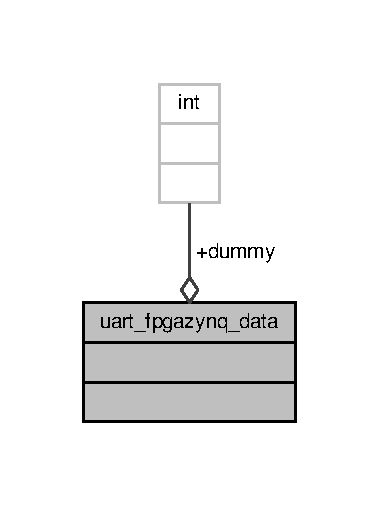
\includegraphics[width=182pt]{structuart__fpgazynq__data__coll__graph}
\end{center}
\end{figure}
\subsection*{Data Fields}
\begin{DoxyCompactItemize}
\item 
int \hyperlink{structuart__fpgazynq__data_a7c1d654b7b6114d7a0abc8d351dd1bcd}{dummy}
\end{DoxyCompactItemize}


\subsection{Field Documentation}
\index{uart\+\_\+fpgazynq\+\_\+data@{uart\+\_\+fpgazynq\+\_\+data}!dummy@{dummy}}
\index{dummy@{dummy}!uart\+\_\+fpgazynq\+\_\+data@{uart\+\_\+fpgazynq\+\_\+data}}
\subsubsection[{\texorpdfstring{dummy}{dummy}}]{\setlength{\rightskip}{0pt plus 5cm}int dummy}\hypertarget{structuart__fpgazynq__data_a7c1d654b7b6114d7a0abc8d351dd1bcd}{}\label{structuart__fpgazynq__data_a7c1d654b7b6114d7a0abc8d351dd1bcd}


The documentation for this struct was generated from the following file\+:\begin{DoxyCompactItemize}
\item 
/home/timo/\+Software/zephyr-\/riscv\+\_\+dev/apps/irqperipheral\+\_\+test/src/drivers/fpga-\/zynq\+\_\+console/src/\hyperlink{uart__fpgazynq_8c}{uart\+\_\+fpgazynq.\+c}\end{DoxyCompactItemize}

\hypertarget{structuart__fpgazynq__device__config}{}\section{uart\+\_\+fpgazynq\+\_\+device\+\_\+config Struct Reference}
\label{structuart__fpgazynq__device__config}\index{uart\+\_\+fpgazynq\+\_\+device\+\_\+config@{uart\+\_\+fpgazynq\+\_\+device\+\_\+config}}


Collaboration diagram for uart\+\_\+fpgazynq\+\_\+device\+\_\+config\+:\nopagebreak
\begin{figure}[H]
\begin{center}
\leavevmode
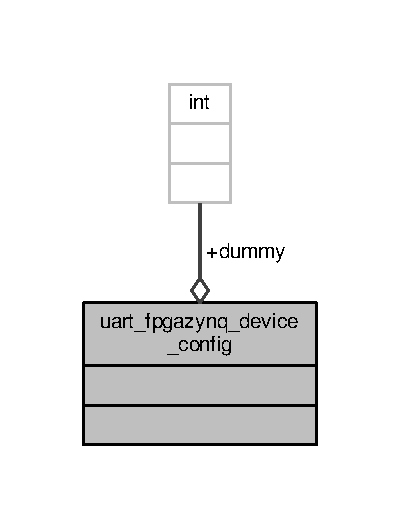
\includegraphics[width=192pt]{structuart__fpgazynq__device__config__coll__graph}
\end{center}
\end{figure}
\subsection*{Data Fields}
\begin{DoxyCompactItemize}
\item 
int \hyperlink{structuart__fpgazynq__device__config_a7c1d654b7b6114d7a0abc8d351dd1bcd}{dummy}
\end{DoxyCompactItemize}


\subsection{Field Documentation}
\index{uart\+\_\+fpgazynq\+\_\+device\+\_\+config@{uart\+\_\+fpgazynq\+\_\+device\+\_\+config}!dummy@{dummy}}
\index{dummy@{dummy}!uart\+\_\+fpgazynq\+\_\+device\+\_\+config@{uart\+\_\+fpgazynq\+\_\+device\+\_\+config}}
\subsubsection[{\texorpdfstring{dummy}{dummy}}]{\setlength{\rightskip}{0pt plus 5cm}int dummy}\hypertarget{structuart__fpgazynq__device__config_a7c1d654b7b6114d7a0abc8d351dd1bcd}{}\label{structuart__fpgazynq__device__config_a7c1d654b7b6114d7a0abc8d351dd1bcd}


The documentation for this struct was generated from the following file\+:\begin{DoxyCompactItemize}
\item 
/home/timo/\+Software/zephyr-\/riscv\+\_\+dev/apps/irqperipheral\+\_\+test/src/drivers/fpga-\/zynq\+\_\+console/src/\hyperlink{uart__fpgazynq_8c}{uart\+\_\+fpgazynq.\+c}\end{DoxyCompactItemize}

\hypertarget{struct_wait___event}{}\section{Wait\+\_\+\+Event Struct Reference}
\label{struct_wait___event}\index{Wait\+\_\+\+Event@{Wait\+\_\+\+Event}}


used for logging  




{\ttfamily \#include $<$state\+\_\+manager.\+h$>$}



Collaboration diagram for Wait\+\_\+\+Event\+:\nopagebreak
\begin{figure}[H]
\begin{center}
\leavevmode
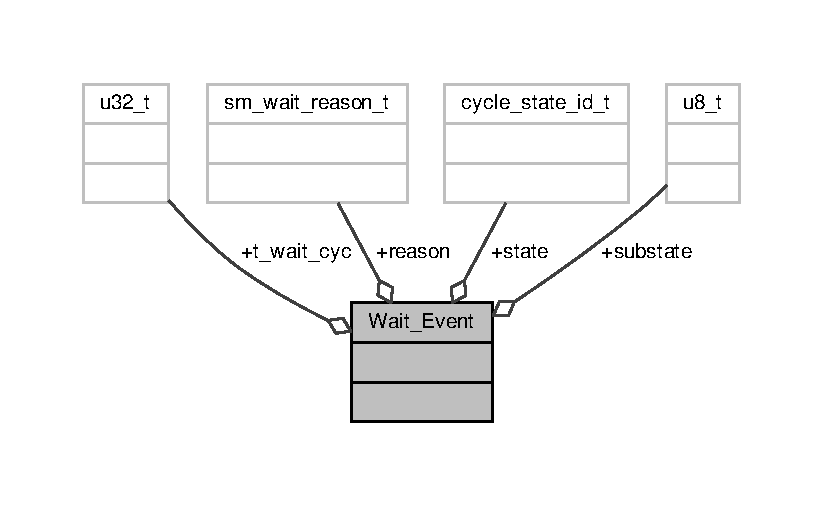
\includegraphics[width=350pt]{struct_wait___event__coll__graph}
\end{center}
\end{figure}
\subsection*{Data Fields}
\begin{DoxyCompactItemize}
\item 
\hyperlink{states_8h_a9e0ef0bc98a491d55216d9485e562252}{cycle\+\_\+state\+\_\+id\+\_\+t} \hyperlink{struct_wait___event_a6ed5d93e163f36fafba6a6fa602ab3f0}{state}
\item 
u8\+\_\+t \hyperlink{struct_wait___event_aa719d2e676dc0eeaafeaae9bbc1849f0}{substate}
\item 
u32\+\_\+t \hyperlink{struct_wait___event_ac0c05f560bacae9a4ff37c4b734c9dae}{t\+\_\+wait\+\_\+cyc}
\item 
\hyperlink{state__manager_8h_ac061587bd504b89ca120f3bb56e6f4e8}{sm\+\_\+wait\+\_\+reason\+\_\+t} \hyperlink{struct_wait___event_a734736de72a0e0b0c1d7cdb3aeb38b67}{reason}
\end{DoxyCompactItemize}


\subsection{Detailed Description}
used for logging 

\subsection{Field Documentation}
\index{Wait\+\_\+\+Event@{Wait\+\_\+\+Event}!reason@{reason}}
\index{reason@{reason}!Wait\+\_\+\+Event@{Wait\+\_\+\+Event}}
\subsubsection[{\texorpdfstring{reason}{reason}}]{\setlength{\rightskip}{0pt plus 5cm}{\bf sm\+\_\+wait\+\_\+reason\+\_\+t} reason}\hypertarget{struct_wait___event_a734736de72a0e0b0c1d7cdb3aeb38b67}{}\label{struct_wait___event_a734736de72a0e0b0c1d7cdb3aeb38b67}
\index{Wait\+\_\+\+Event@{Wait\+\_\+\+Event}!state@{state}}
\index{state@{state}!Wait\+\_\+\+Event@{Wait\+\_\+\+Event}}
\subsubsection[{\texorpdfstring{state}{state}}]{\setlength{\rightskip}{0pt plus 5cm}{\bf cycle\+\_\+state\+\_\+id\+\_\+t} state}\hypertarget{struct_wait___event_a6ed5d93e163f36fafba6a6fa602ab3f0}{}\label{struct_wait___event_a6ed5d93e163f36fafba6a6fa602ab3f0}
\index{Wait\+\_\+\+Event@{Wait\+\_\+\+Event}!substate@{substate}}
\index{substate@{substate}!Wait\+\_\+\+Event@{Wait\+\_\+\+Event}}
\subsubsection[{\texorpdfstring{substate}{substate}}]{\setlength{\rightskip}{0pt plus 5cm}u8\+\_\+t substate}\hypertarget{struct_wait___event_aa719d2e676dc0eeaafeaae9bbc1849f0}{}\label{struct_wait___event_aa719d2e676dc0eeaafeaae9bbc1849f0}
\index{Wait\+\_\+\+Event@{Wait\+\_\+\+Event}!t\+\_\+wait\+\_\+cyc@{t\+\_\+wait\+\_\+cyc}}
\index{t\+\_\+wait\+\_\+cyc@{t\+\_\+wait\+\_\+cyc}!Wait\+\_\+\+Event@{Wait\+\_\+\+Event}}
\subsubsection[{\texorpdfstring{t\+\_\+wait\+\_\+cyc}{t_wait_cyc}}]{\setlength{\rightskip}{0pt plus 5cm}u32\+\_\+t t\+\_\+wait\+\_\+cyc}\hypertarget{struct_wait___event_ac0c05f560bacae9a4ff37c4b734c9dae}{}\label{struct_wait___event_ac0c05f560bacae9a4ff37c4b734c9dae}


The documentation for this struct was generated from the following file\+:\begin{DoxyCompactItemize}
\item 
/home/timo/\+Software/zephyr-\/riscv\+\_\+dev/apps/irqperipheral\+\_\+test/src/\hyperlink{state__manager_8h}{state\+\_\+manager.\+h}\end{DoxyCompactItemize}

\chapter{File Documentation}
\hypertarget{cycles_8c}{}\section{/home/timo/\+Software/zephyr-\/riscv\+\_\+dev/apps/irqperipheral\+\_\+test/src/drivers/common/cycles.c File Reference}
\label{cycles_8c}\index{/home/timo/\+Software/zephyr-\/riscv\+\_\+dev/apps/irqperipheral\+\_\+test/src/drivers/common/cycles.\+c@{/home/timo/\+Software/zephyr-\/riscv\+\_\+dev/apps/irqperipheral\+\_\+test/src/drivers/common/cycles.\+c}}
{\ttfamily \#include \char`\"{}cycles.\+h\char`\"{}}\\*
{\ttfamily \#include $<$stdio.\+h$>$}\\*
{\ttfamily \#include \char`\"{}encoding.\+h\char`\"{}}\\*
Include dependency graph for cycles.\+c\+:\nopagebreak
\begin{figure}[H]
\begin{center}
\leavevmode
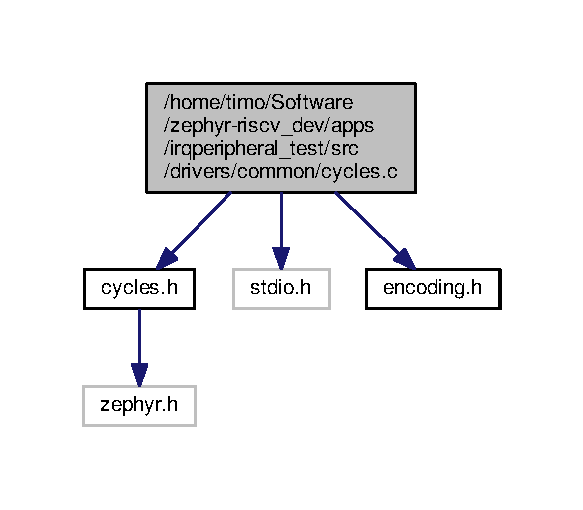
\includegraphics[width=280pt]{cycles_8c__incl}
\end{center}
\end{figure}
\subsection*{Macros}
\begin{DoxyCompactItemize}
\item 
\#define \hyperlink{cycles_8c_aac84bff3e1706bfb386438251534a5ac}{C\+Y\+C\+L\+E\+S\+\_\+\+C\+P\+U\+C\+Y\+C\+\_\+\+P\+E\+R\+\_\+\+US}~C\+O\+N\+F\+I\+G\+\_\+\+A\+P\+P\+\_\+\+R\+I\+S\+C\+V\+\_\+\+C\+O\+R\+E\+\_\+\+F\+R\+E\+Q\+\_\+\+M\+HZ
\item 
\#define \hyperlink{cycles_8c_a178bb1b90da326048e8c83b4515768be}{rdmcycle}(x)
\end{DoxyCompactItemize}
\subsection*{Functions}
\begin{DoxyCompactItemize}
\item 
u32\+\_\+t \hyperlink{cycles_8c_a6e9f891bc6d1b4849bd701cca50ef426}{get\+\_\+cycle\+\_\+32} ()
\begin{DoxyCompactList}\small\item\em read lower 32 bits of cycle csr register \end{DoxyCompactList}\item 
void \hyperlink{cycles_8c_a8bf6852b90b5cdddf4be52c673ddd590}{cycle\+\_\+busy\+\_\+wait} (u32\+\_\+t t\+\_\+cyc)
\begin{DoxyCompactList}\small\item\em Wait for at least t\+\_\+cyc cpu cycles. \end{DoxyCompactList}\item 
u32\+\_\+t \hyperlink{cycles_8c_af94426e16139d6b6dd6b7c7f1aad5180}{cycle\+\_\+us\+\_\+2\+\_\+cyc} (u32\+\_\+t t\+\_\+us)
\item 
u32\+\_\+t \hyperlink{cycles_8c_a373d9d4b93bfff07d053e7cfaf17b42d}{cycle\+\_\+cyc\+\_\+2\+\_\+us} (u32\+\_\+t t\+\_\+cyc)
\begin{DoxyCompactList}\small\item\em Attention\+: result is rounded. \end{DoxyCompactList}\end{DoxyCompactItemize}


\subsection{Macro Definition Documentation}
\index{cycles.\+c@{cycles.\+c}!C\+Y\+C\+L\+E\+S\+\_\+\+C\+P\+U\+C\+Y\+C\+\_\+\+P\+E\+R\+\_\+\+US@{C\+Y\+C\+L\+E\+S\+\_\+\+C\+P\+U\+C\+Y\+C\+\_\+\+P\+E\+R\+\_\+\+US}}
\index{C\+Y\+C\+L\+E\+S\+\_\+\+C\+P\+U\+C\+Y\+C\+\_\+\+P\+E\+R\+\_\+\+US@{C\+Y\+C\+L\+E\+S\+\_\+\+C\+P\+U\+C\+Y\+C\+\_\+\+P\+E\+R\+\_\+\+US}!cycles.\+c@{cycles.\+c}}
\subsubsection[{\texorpdfstring{C\+Y\+C\+L\+E\+S\+\_\+\+C\+P\+U\+C\+Y\+C\+\_\+\+P\+E\+R\+\_\+\+US}{CYCLES_CPUCYC_PER_US}}]{\setlength{\rightskip}{0pt plus 5cm}\#define C\+Y\+C\+L\+E\+S\+\_\+\+C\+P\+U\+C\+Y\+C\+\_\+\+P\+E\+R\+\_\+\+US~C\+O\+N\+F\+I\+G\+\_\+\+A\+P\+P\+\_\+\+R\+I\+S\+C\+V\+\_\+\+C\+O\+R\+E\+\_\+\+F\+R\+E\+Q\+\_\+\+M\+HZ}\hypertarget{cycles_8c_aac84bff3e1706bfb386438251534a5ac}{}\label{cycles_8c_aac84bff3e1706bfb386438251534a5ac}
\index{cycles.\+c@{cycles.\+c}!rdmcycle@{rdmcycle}}
\index{rdmcycle@{rdmcycle}!cycles.\+c@{cycles.\+c}}
\subsubsection[{\texorpdfstring{rdmcycle}{rdmcycle}}]{\setlength{\rightskip}{0pt plus 5cm}\#define rdmcycle(
\begin{DoxyParamCaption}
\item[{}]{x}
\end{DoxyParamCaption}
)}\hypertarget{cycles_8c_a178bb1b90da326048e8c83b4515768be}{}\label{cycles_8c_a178bb1b90da326048e8c83b4515768be}
{\bfseries Value\+:}
\begin{DoxyCode}
(\{                     \(\backslash\)
    uint32\_t lo, hi, hi2;                  \(\backslash\)
    \_\_asm\_\_ \_\_volatile\_\_ (\textcolor{stringliteral}{"1:\(\backslash\)n\(\backslash\)t"}             \(\backslash\)
              \textcolor{stringliteral}{"csrr %0, mcycleh\(\backslash\)n\(\backslash\)t"}       \(\backslash\)
              \textcolor{stringliteral}{"csrr %1, mcycle\(\backslash\)n\(\backslash\)t"}        \(\backslash\)
              \textcolor{stringliteral}{"csrr %2, mcycleh\(\backslash\)n\(\backslash\)t"}       \(\backslash\)
              \textcolor{stringliteral}{"bne  %0, %2, 1b\(\backslash\)n\(\backslash\)t"}         \(\backslash\)
              : \textcolor{stringliteral}{"=r"} (hi), \textcolor{stringliteral}{"=r"} (lo), \textcolor{stringliteral}{"=r"} (hi2)) ; \(\backslash\)
    *(x) = lo | ((uint64\_t) hi << 32);              \(\backslash\)
\})
\end{DoxyCode}


\subsection{Function Documentation}
\index{cycles.\+c@{cycles.\+c}!cycle\+\_\+busy\+\_\+wait@{cycle\+\_\+busy\+\_\+wait}}
\index{cycle\+\_\+busy\+\_\+wait@{cycle\+\_\+busy\+\_\+wait}!cycles.\+c@{cycles.\+c}}
\subsubsection[{\texorpdfstring{cycle\+\_\+busy\+\_\+wait(u32\+\_\+t t\+\_\+cyc)}{cycle_busy_wait(u32_t t_cyc)}}]{\setlength{\rightskip}{0pt plus 5cm}void cycle\+\_\+busy\+\_\+wait (
\begin{DoxyParamCaption}
\item[{u32\+\_\+t}]{t\+\_\+cyc}
\end{DoxyParamCaption}
)}\hypertarget{cycles_8c_a8bf6852b90b5cdddf4be52c673ddd590}{}\label{cycles_8c_a8bf6852b90b5cdddf4be52c673ddd590}


Wait for at least t\+\_\+cyc cpu cycles. 

No upper limit of waiting time guaranteed! Busy waiting currently, since no hw timers implemented yet. 

Here is the call graph for this function\+:\nopagebreak
\begin{figure}[H]
\begin{center}
\leavevmode
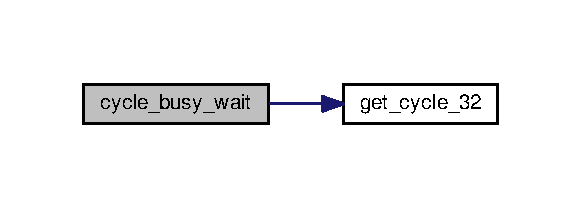
\includegraphics[width=279pt]{cycles_8c_a8bf6852b90b5cdddf4be52c673ddd590_cgraph}
\end{center}
\end{figure}


\index{cycles.\+c@{cycles.\+c}!cycle\+\_\+cyc\+\_\+2\+\_\+us@{cycle\+\_\+cyc\+\_\+2\+\_\+us}}
\index{cycle\+\_\+cyc\+\_\+2\+\_\+us@{cycle\+\_\+cyc\+\_\+2\+\_\+us}!cycles.\+c@{cycles.\+c}}
\subsubsection[{\texorpdfstring{cycle\+\_\+cyc\+\_\+2\+\_\+us(u32\+\_\+t t\+\_\+cyc)}{cycle_cyc_2_us(u32_t t_cyc)}}]{\setlength{\rightskip}{0pt plus 5cm}u32\+\_\+t cycle\+\_\+cyc\+\_\+2\+\_\+us (
\begin{DoxyParamCaption}
\item[{u32\+\_\+t}]{t\+\_\+cyc}
\end{DoxyParamCaption}
)}\hypertarget{cycles_8c_a373d9d4b93bfff07d053e7cfaf17b42d}{}\label{cycles_8c_a373d9d4b93bfff07d053e7cfaf17b42d}


Attention\+: result is rounded. 

\index{cycles.\+c@{cycles.\+c}!cycle\+\_\+us\+\_\+2\+\_\+cyc@{cycle\+\_\+us\+\_\+2\+\_\+cyc}}
\index{cycle\+\_\+us\+\_\+2\+\_\+cyc@{cycle\+\_\+us\+\_\+2\+\_\+cyc}!cycles.\+c@{cycles.\+c}}
\subsubsection[{\texorpdfstring{cycle\+\_\+us\+\_\+2\+\_\+cyc(u32\+\_\+t t\+\_\+us)}{cycle_us_2_cyc(u32_t t_us)}}]{\setlength{\rightskip}{0pt plus 5cm}u32\+\_\+t cycle\+\_\+us\+\_\+2\+\_\+cyc (
\begin{DoxyParamCaption}
\item[{u32\+\_\+t}]{t\+\_\+us}
\end{DoxyParamCaption}
)}\hypertarget{cycles_8c_af94426e16139d6b6dd6b7c7f1aad5180}{}\label{cycles_8c_af94426e16139d6b6dd6b7c7f1aad5180}
\index{cycles.\+c@{cycles.\+c}!get\+\_\+cycle\+\_\+32@{get\+\_\+cycle\+\_\+32}}
\index{get\+\_\+cycle\+\_\+32@{get\+\_\+cycle\+\_\+32}!cycles.\+c@{cycles.\+c}}
\subsubsection[{\texorpdfstring{get\+\_\+cycle\+\_\+32()}{get_cycle_32()}}]{\setlength{\rightskip}{0pt plus 5cm}u32\+\_\+t get\+\_\+cycle\+\_\+32 (
\begin{DoxyParamCaption}
{}
\end{DoxyParamCaption}
)}\hypertarget{cycles_8c_a6e9f891bc6d1b4849bd701cca50ef426}{}\label{cycles_8c_a6e9f891bc6d1b4849bd701cca50ef426}


read lower 32 bits of cycle csr register 


\hypertarget{cycles_8h}{}\section{/home/timo/\+Software/zephyr-\/riscv\+\_\+dev/apps/irqperipheral\+\_\+test/src/drivers/common/cycles.h File Reference}
\label{cycles_8h}\index{/home/timo/\+Software/zephyr-\/riscv\+\_\+dev/apps/irqperipheral\+\_\+test/src/drivers/common/cycles.\+h@{/home/timo/\+Software/zephyr-\/riscv\+\_\+dev/apps/irqperipheral\+\_\+test/src/drivers/common/cycles.\+h}}


Deal with riscv32 hardware cpu cycles.  


{\ttfamily \#include $<$zephyr.\+h$>$}\\*
Include dependency graph for cycles.\+h\+:\nopagebreak
\begin{figure}[H]
\begin{center}
\leavevmode
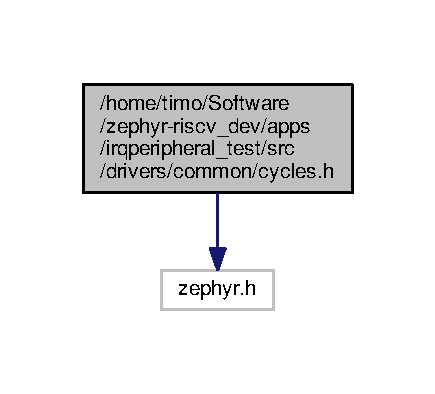
\includegraphics[width=209pt]{cycles_8h__incl}
\end{center}
\end{figure}
This graph shows which files directly or indirectly include this file\+:
\nopagebreak
\begin{figure}[H]
\begin{center}
\leavevmode
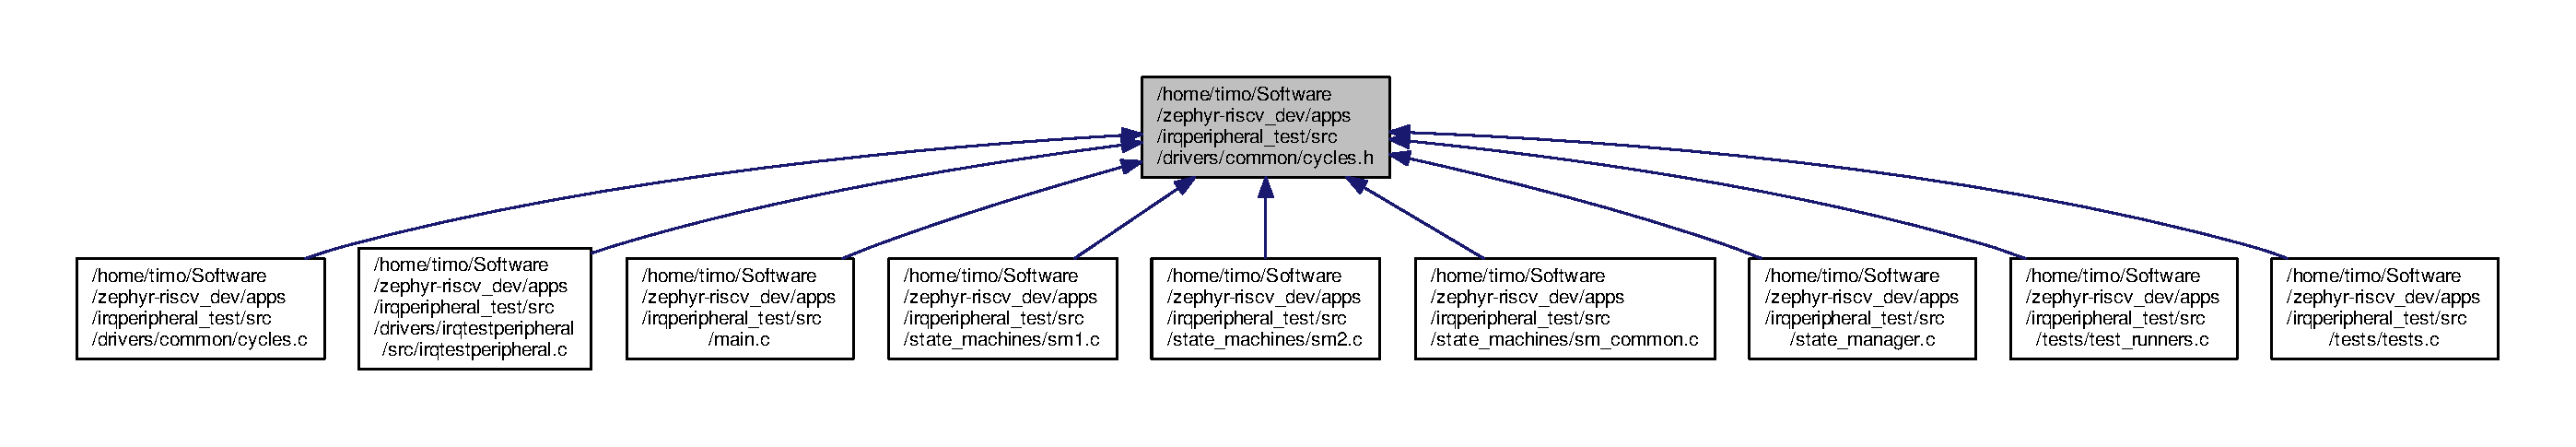
\includegraphics[width=350pt]{cycles_8h__dep__incl}
\end{center}
\end{figure}
\subsection*{Macros}
\begin{DoxyCompactItemize}
\item 
\#define \hyperlink{cycles_8h_a7ade2b760aa6a5f5d65cca4d30adee63}{C\+Y\+C\+L\+E\+S\+\_\+\+C\+Y\+C\+\_\+2\+\_\+\+MS}(t\+\_\+cyc)~(t\+\_\+cyc $<$= 1000$\ast$C\+O\+N\+F\+I\+G\+\_\+\+A\+P\+P\+\_\+\+R\+I\+S\+C\+V\+\_\+\+C\+O\+R\+E\+\_\+\+F\+R\+E\+Q\+\_\+\+M\+HZ ? 1 \+: (t\+\_\+cyc / (1000$\ast$C\+O\+N\+F\+I\+G\+\_\+\+A\+P\+P\+\_\+\+R\+I\+S\+C\+V\+\_\+\+C\+O\+R\+E\+\_\+\+F\+R\+E\+Q\+\_\+\+M\+HZ)))
\begin{DoxyCompactList}\small\item\em Convert cpu cycles to integer milliseconds $>$= 1. \end{DoxyCompactList}\item 
\#define \hyperlink{cycles_8h_a9e1c6f161f9d0713a85aba42a5642216}{C\+Y\+C\+L\+E\+S\+\_\+\+C\+Y\+C\+\_\+2\+\_\+\+US}(t\+\_\+cyc)~(t\+\_\+cyc $<$= C\+O\+N\+F\+I\+G\+\_\+\+A\+P\+P\+\_\+\+R\+I\+S\+C\+V\+\_\+\+C\+O\+R\+E\+\_\+\+F\+R\+E\+Q\+\_\+\+M\+HZ ? 1 \+: (t\+\_\+cyc / (C\+O\+N\+F\+I\+G\+\_\+\+A\+P\+P\+\_\+\+R\+I\+S\+C\+V\+\_\+\+C\+O\+R\+E\+\_\+\+F\+R\+E\+Q\+\_\+\+M\+HZ)))
\item 
\#define \hyperlink{cycles_8h_a70282809bd2123435ba13a5fea81f8ff}{C\+Y\+C\+L\+E\+S\+\_\+\+M\+S\+\_\+2\+\_\+\+C\+YC}(t\+\_\+ms)~(1000$\ast$C\+O\+N\+F\+I\+G\+\_\+\+A\+P\+P\+\_\+\+R\+I\+S\+C\+V\+\_\+\+C\+O\+R\+E\+\_\+\+F\+R\+E\+Q\+\_\+\+M\+HZ $\ast$ t\+\_\+ms)
\begin{DoxyCompactList}\small\item\em Convert milliseconds to cpu cycles $>$= 1. \end{DoxyCompactList}\item 
\#define \hyperlink{cycles_8h_a6f50f35dad955420fed104b8b8a0678d}{C\+Y\+C\+L\+E\+S\+\_\+\+U\+S\+\_\+2\+\_\+\+C\+YC}(t\+\_\+ms)~(C\+O\+N\+F\+I\+G\+\_\+\+A\+P\+P\+\_\+\+R\+I\+S\+C\+V\+\_\+\+C\+O\+R\+E\+\_\+\+F\+R\+E\+Q\+\_\+\+M\+HZ $\ast$ t\+\_\+ms)
\end{DoxyCompactItemize}
\subsection*{Functions}
\begin{DoxyCompactItemize}
\item 
u32\+\_\+t \hyperlink{cycles_8h_a6e9f891bc6d1b4849bd701cca50ef426}{get\+\_\+cycle\+\_\+32} ()
\begin{DoxyCompactList}\small\item\em read lower 32 bits of cycle csr register \end{DoxyCompactList}\item 
void \hyperlink{cycles_8h_a8bf6852b90b5cdddf4be52c673ddd590}{cycle\+\_\+busy\+\_\+wait} (u32\+\_\+t t\+\_\+cyc)
\begin{DoxyCompactList}\small\item\em Wait for at least t\+\_\+cyc cpu cycles. \end{DoxyCompactList}\end{DoxyCompactItemize}


\subsection{Detailed Description}
Deal with riscv32 hardware cpu cycles. 

Extension to macros in sys\+\_\+cloch.\+h for cpu cycle based units. Mind the difference between sysclock (or rtc) cycles and cpu cycles! 

\subsection{Macro Definition Documentation}
\index{cycles.\+h@{cycles.\+h}!C\+Y\+C\+L\+E\+S\+\_\+\+C\+Y\+C\+\_\+2\+\_\+\+MS@{C\+Y\+C\+L\+E\+S\+\_\+\+C\+Y\+C\+\_\+2\+\_\+\+MS}}
\index{C\+Y\+C\+L\+E\+S\+\_\+\+C\+Y\+C\+\_\+2\+\_\+\+MS@{C\+Y\+C\+L\+E\+S\+\_\+\+C\+Y\+C\+\_\+2\+\_\+\+MS}!cycles.\+h@{cycles.\+h}}
\subsubsection[{\texorpdfstring{C\+Y\+C\+L\+E\+S\+\_\+\+C\+Y\+C\+\_\+2\+\_\+\+MS}{CYCLES_CYC_2_MS}}]{\setlength{\rightskip}{0pt plus 5cm}\#define C\+Y\+C\+L\+E\+S\+\_\+\+C\+Y\+C\+\_\+2\+\_\+\+MS(
\begin{DoxyParamCaption}
\item[{}]{t\+\_\+cyc}
\end{DoxyParamCaption}
)~(t\+\_\+cyc $<$= 1000$\ast$C\+O\+N\+F\+I\+G\+\_\+\+A\+P\+P\+\_\+\+R\+I\+S\+C\+V\+\_\+\+C\+O\+R\+E\+\_\+\+F\+R\+E\+Q\+\_\+\+M\+HZ ? 1 \+: (t\+\_\+cyc / (1000$\ast$C\+O\+N\+F\+I\+G\+\_\+\+A\+P\+P\+\_\+\+R\+I\+S\+C\+V\+\_\+\+C\+O\+R\+E\+\_\+\+F\+R\+E\+Q\+\_\+\+M\+HZ)))}\hypertarget{cycles_8h_a7ade2b760aa6a5f5d65cca4d30adee63}{}\label{cycles_8h_a7ade2b760aa6a5f5d65cca4d30adee63}


Convert cpu cycles to integer milliseconds $>$= 1. 

Warning\+: Cpu cycles are less accurate than sysclock cycles! \index{cycles.\+h@{cycles.\+h}!C\+Y\+C\+L\+E\+S\+\_\+\+C\+Y\+C\+\_\+2\+\_\+\+US@{C\+Y\+C\+L\+E\+S\+\_\+\+C\+Y\+C\+\_\+2\+\_\+\+US}}
\index{C\+Y\+C\+L\+E\+S\+\_\+\+C\+Y\+C\+\_\+2\+\_\+\+US@{C\+Y\+C\+L\+E\+S\+\_\+\+C\+Y\+C\+\_\+2\+\_\+\+US}!cycles.\+h@{cycles.\+h}}
\subsubsection[{\texorpdfstring{C\+Y\+C\+L\+E\+S\+\_\+\+C\+Y\+C\+\_\+2\+\_\+\+US}{CYCLES_CYC_2_US}}]{\setlength{\rightskip}{0pt plus 5cm}\#define C\+Y\+C\+L\+E\+S\+\_\+\+C\+Y\+C\+\_\+2\+\_\+\+US(
\begin{DoxyParamCaption}
\item[{}]{t\+\_\+cyc}
\end{DoxyParamCaption}
)~(t\+\_\+cyc $<$= C\+O\+N\+F\+I\+G\+\_\+\+A\+P\+P\+\_\+\+R\+I\+S\+C\+V\+\_\+\+C\+O\+R\+E\+\_\+\+F\+R\+E\+Q\+\_\+\+M\+HZ ? 1 \+: (t\+\_\+cyc / (C\+O\+N\+F\+I\+G\+\_\+\+A\+P\+P\+\_\+\+R\+I\+S\+C\+V\+\_\+\+C\+O\+R\+E\+\_\+\+F\+R\+E\+Q\+\_\+\+M\+HZ)))}\hypertarget{cycles_8h_a9e1c6f161f9d0713a85aba42a5642216}{}\label{cycles_8h_a9e1c6f161f9d0713a85aba42a5642216}
\index{cycles.\+h@{cycles.\+h}!C\+Y\+C\+L\+E\+S\+\_\+\+M\+S\+\_\+2\+\_\+\+C\+YC@{C\+Y\+C\+L\+E\+S\+\_\+\+M\+S\+\_\+2\+\_\+\+C\+YC}}
\index{C\+Y\+C\+L\+E\+S\+\_\+\+M\+S\+\_\+2\+\_\+\+C\+YC@{C\+Y\+C\+L\+E\+S\+\_\+\+M\+S\+\_\+2\+\_\+\+C\+YC}!cycles.\+h@{cycles.\+h}}
\subsubsection[{\texorpdfstring{C\+Y\+C\+L\+E\+S\+\_\+\+M\+S\+\_\+2\+\_\+\+C\+YC}{CYCLES_MS_2_CYC}}]{\setlength{\rightskip}{0pt plus 5cm}\#define C\+Y\+C\+L\+E\+S\+\_\+\+M\+S\+\_\+2\+\_\+\+C\+YC(
\begin{DoxyParamCaption}
\item[{}]{t\+\_\+ms}
\end{DoxyParamCaption}
)~(1000$\ast$C\+O\+N\+F\+I\+G\+\_\+\+A\+P\+P\+\_\+\+R\+I\+S\+C\+V\+\_\+\+C\+O\+R\+E\+\_\+\+F\+R\+E\+Q\+\_\+\+M\+HZ $\ast$ t\+\_\+ms)}\hypertarget{cycles_8h_a70282809bd2123435ba13a5fea81f8ff}{}\label{cycles_8h_a70282809bd2123435ba13a5fea81f8ff}


Convert milliseconds to cpu cycles $>$= 1. 

Warning\+: Cpu cycles are less accurate than sysclock cycles! \index{cycles.\+h@{cycles.\+h}!C\+Y\+C\+L\+E\+S\+\_\+\+U\+S\+\_\+2\+\_\+\+C\+YC@{C\+Y\+C\+L\+E\+S\+\_\+\+U\+S\+\_\+2\+\_\+\+C\+YC}}
\index{C\+Y\+C\+L\+E\+S\+\_\+\+U\+S\+\_\+2\+\_\+\+C\+YC@{C\+Y\+C\+L\+E\+S\+\_\+\+U\+S\+\_\+2\+\_\+\+C\+YC}!cycles.\+h@{cycles.\+h}}
\subsubsection[{\texorpdfstring{C\+Y\+C\+L\+E\+S\+\_\+\+U\+S\+\_\+2\+\_\+\+C\+YC}{CYCLES_US_2_CYC}}]{\setlength{\rightskip}{0pt plus 5cm}\#define C\+Y\+C\+L\+E\+S\+\_\+\+U\+S\+\_\+2\+\_\+\+C\+YC(
\begin{DoxyParamCaption}
\item[{}]{t\+\_\+ms}
\end{DoxyParamCaption}
)~(C\+O\+N\+F\+I\+G\+\_\+\+A\+P\+P\+\_\+\+R\+I\+S\+C\+V\+\_\+\+C\+O\+R\+E\+\_\+\+F\+R\+E\+Q\+\_\+\+M\+HZ $\ast$ t\+\_\+ms)}\hypertarget{cycles_8h_a6f50f35dad955420fed104b8b8a0678d}{}\label{cycles_8h_a6f50f35dad955420fed104b8b8a0678d}


\subsection{Function Documentation}
\index{cycles.\+h@{cycles.\+h}!cycle\+\_\+busy\+\_\+wait@{cycle\+\_\+busy\+\_\+wait}}
\index{cycle\+\_\+busy\+\_\+wait@{cycle\+\_\+busy\+\_\+wait}!cycles.\+h@{cycles.\+h}}
\subsubsection[{\texorpdfstring{cycle\+\_\+busy\+\_\+wait(u32\+\_\+t t\+\_\+cyc)}{cycle_busy_wait(u32_t t_cyc)}}]{\setlength{\rightskip}{0pt plus 5cm}void cycle\+\_\+busy\+\_\+wait (
\begin{DoxyParamCaption}
\item[{u32\+\_\+t}]{t\+\_\+cyc}
\end{DoxyParamCaption}
)}\hypertarget{cycles_8h_a8bf6852b90b5cdddf4be52c673ddd590}{}\label{cycles_8h_a8bf6852b90b5cdddf4be52c673ddd590}


Wait for at least t\+\_\+cyc cpu cycles. 

No upper limit of waiting time guaranteed! Busy waiting currently, since no hw timers implemented yet. 

Here is the call graph for this function\+:\nopagebreak
\begin{figure}[H]
\begin{center}
\leavevmode
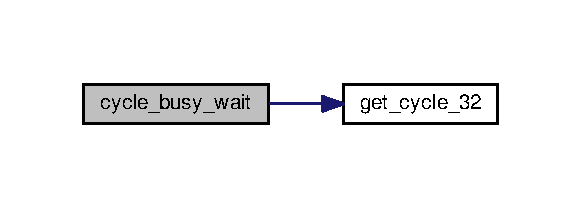
\includegraphics[width=279pt]{cycles_8h_a8bf6852b90b5cdddf4be52c673ddd590_cgraph}
\end{center}
\end{figure}


\index{cycles.\+h@{cycles.\+h}!get\+\_\+cycle\+\_\+32@{get\+\_\+cycle\+\_\+32}}
\index{get\+\_\+cycle\+\_\+32@{get\+\_\+cycle\+\_\+32}!cycles.\+h@{cycles.\+h}}
\subsubsection[{\texorpdfstring{get\+\_\+cycle\+\_\+32()}{get_cycle_32()}}]{\setlength{\rightskip}{0pt plus 5cm}u32\+\_\+t get\+\_\+cycle\+\_\+32 (
\begin{DoxyParamCaption}
{}
\end{DoxyParamCaption}
)}\hypertarget{cycles_8h_a6e9f891bc6d1b4849bd701cca50ef426}{}\label{cycles_8h_a6e9f891bc6d1b4849bd701cca50ef426}


read lower 32 bits of cycle csr register 


\hypertarget{drivers_2common_2encoding_8h}{}\section{/home/timo/\+Software/zephyr-\/riscv\+\_\+dev/apps/irqperipheral\+\_\+test/src/drivers/common/encoding.h File Reference}
\label{drivers_2common_2encoding_8h}\index{/home/timo/\+Software/zephyr-\/riscv\+\_\+dev/apps/irqperipheral\+\_\+test/src/drivers/common/encoding.\+h@{/home/timo/\+Software/zephyr-\/riscv\+\_\+dev/apps/irqperipheral\+\_\+test/src/drivers/common/encoding.\+h}}
This graph shows which files directly or indirectly include this file\+:\nopagebreak
\begin{figure}[H]
\begin{center}
\leavevmode
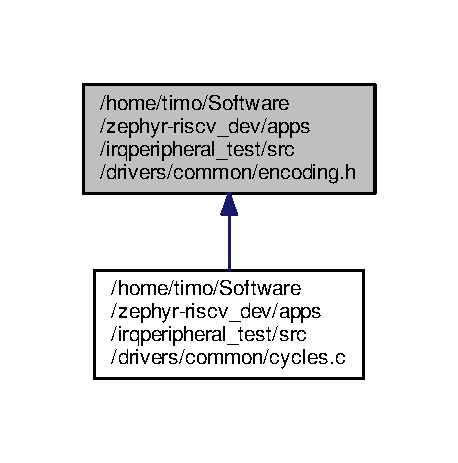
\includegraphics[width=220pt]{drivers_2common_2encoding_8h__dep__incl}
\end{center}
\end{figure}
\subsection*{Macros}
\begin{DoxyCompactItemize}
\item 
\#define \hyperlink{drivers_2common_2encoding_8h_a3f4df6dc4219593cb6e8bd13d636e844}{M\+S\+T\+A\+T\+U\+S\+\_\+\+U\+IE}~0x00000001
\item 
\#define \hyperlink{drivers_2common_2encoding_8h_a29a63dca3cfcf13877a0c354dc081505}{M\+S\+T\+A\+T\+U\+S\+\_\+\+S\+IE}~0x00000002
\item 
\#define \hyperlink{drivers_2common_2encoding_8h_ab549408c2d03c2e09fbfab2898683097}{M\+S\+T\+A\+T\+U\+S\+\_\+\+H\+IE}~0x00000004
\item 
\#define \hyperlink{drivers_2common_2encoding_8h_a225cb34e3b991318fa87f090cfc3fc5f}{M\+S\+T\+A\+T\+U\+S\+\_\+\+M\+IE}~0x00000008
\item 
\#define \hyperlink{drivers_2common_2encoding_8h_a17711b78183c43687036c60962c278cb}{M\+S\+T\+A\+T\+U\+S\+\_\+\+U\+P\+IE}~0x00000010
\item 
\#define \hyperlink{drivers_2common_2encoding_8h_ac7fef7988d408f1f4ebe9e3849d68bb2}{M\+S\+T\+A\+T\+U\+S\+\_\+\+S\+P\+IE}~0x00000020
\item 
\#define \hyperlink{drivers_2common_2encoding_8h_aa0f7327c94aa1210a819f1d47d3e1700}{M\+S\+T\+A\+T\+U\+S\+\_\+\+H\+P\+IE}~0x00000040
\item 
\#define \hyperlink{drivers_2common_2encoding_8h_a05fc511bb3d22b5e1abe8b9ccb30e7b3}{M\+S\+T\+A\+T\+U\+S\+\_\+\+M\+P\+IE}~0x00000080
\item 
\#define \hyperlink{drivers_2common_2encoding_8h_ad4b09023ff5bcbb14192e845c0532944}{M\+S\+T\+A\+T\+U\+S\+\_\+\+S\+PP}~0x00000100
\item 
\#define \hyperlink{drivers_2common_2encoding_8h_ad980a627f9de5aed42de70d2ec617a70}{M\+S\+T\+A\+T\+U\+S\+\_\+\+H\+PP}~0x00000600
\item 
\#define \hyperlink{drivers_2common_2encoding_8h_a2acf460f4ceda869c88c00878cb44314}{M\+S\+T\+A\+T\+U\+S\+\_\+\+M\+PP}~0x00001800
\item 
\#define \hyperlink{drivers_2common_2encoding_8h_ab7b9c10a700f7570d44c49f369b6fcce}{M\+S\+T\+A\+T\+U\+S\+\_\+\+FS}~0x00006000
\item 
\#define \hyperlink{drivers_2common_2encoding_8h_a768db67b06c8341a4da264abcb7f3cfe}{M\+S\+T\+A\+T\+U\+S\+\_\+\+XS}~0x00018000
\item 
\#define \hyperlink{drivers_2common_2encoding_8h_afa733f6d7aadab5b3c0318d005745a98}{M\+S\+T\+A\+T\+U\+S\+\_\+\+M\+P\+RV}~0x00020000
\item 
\#define \hyperlink{drivers_2common_2encoding_8h_a035dd52dddf83c12b5e2bf7c819e54e6}{M\+S\+T\+A\+T\+U\+S\+\_\+\+P\+UM}~0x00040000
\item 
\#define \hyperlink{drivers_2common_2encoding_8h_a8f4b37cdd71162f5b7adb583010443cb}{M\+S\+T\+A\+T\+U\+S\+\_\+\+M\+XR}~0x00080000
\item 
\#define \hyperlink{drivers_2common_2encoding_8h_aa4bb5c6a2a139c0bfd77d4d5de00e8b6}{M\+S\+T\+A\+T\+U\+S\+\_\+\+VM}~0x1\+F000000
\item 
\#define \hyperlink{drivers_2common_2encoding_8h_acca6e5c4f8af666a9b299af295f43348}{M\+S\+T\+A\+T\+U\+S32\+\_\+\+SD}~0x80000000
\item 
\#define \hyperlink{drivers_2common_2encoding_8h_a9d7df82e40e8cf00821e97a0bb8db04e}{M\+S\+T\+A\+T\+U\+S64\+\_\+\+SD}~0x8000000000000000
\item 
\#define \hyperlink{drivers_2common_2encoding_8h_a431c67f7f0e4b5dbdf2048310ad814e0}{S\+S\+T\+A\+T\+U\+S\+\_\+\+U\+IE}~0x00000001
\item 
\#define \hyperlink{drivers_2common_2encoding_8h_a1c1f1da0ecfca5bc4fc4db3acadf1bc8}{S\+S\+T\+A\+T\+U\+S\+\_\+\+S\+IE}~0x00000002
\item 
\#define \hyperlink{drivers_2common_2encoding_8h_a796ad1a8b2314776082e72e13f4a30cf}{S\+S\+T\+A\+T\+U\+S\+\_\+\+U\+P\+IE}~0x00000010
\item 
\#define \hyperlink{drivers_2common_2encoding_8h_a3f9373ba6db2ce5e5c7ea28c2a5b3df9}{S\+S\+T\+A\+T\+U\+S\+\_\+\+S\+P\+IE}~0x00000020
\item 
\#define \hyperlink{drivers_2common_2encoding_8h_a4d0820d6a8b0c5b0fef6875a985d3370}{S\+S\+T\+A\+T\+U\+S\+\_\+\+S\+PP}~0x00000100
\item 
\#define \hyperlink{drivers_2common_2encoding_8h_aff201911cccf15e446c43ba67b0f1aa7}{S\+S\+T\+A\+T\+U\+S\+\_\+\+FS}~0x00006000
\item 
\#define \hyperlink{drivers_2common_2encoding_8h_a2abef254823774927e3bf6b029fbad9d}{S\+S\+T\+A\+T\+U\+S\+\_\+\+XS}~0x00018000
\item 
\#define \hyperlink{drivers_2common_2encoding_8h_af95f0e6f382a6cd93ba925c62d64fe97}{S\+S\+T\+A\+T\+U\+S\+\_\+\+P\+UM}~0x00040000
\item 
\#define \hyperlink{drivers_2common_2encoding_8h_a5f2248b3f4a648ce63c0468a92132971}{S\+S\+T\+A\+T\+U\+S32\+\_\+\+SD}~0x80000000
\item 
\#define \hyperlink{drivers_2common_2encoding_8h_a517c9ab9421f99b99f5da4d549177f38}{S\+S\+T\+A\+T\+U\+S64\+\_\+\+SD}~0x8000000000000000
\item 
\#define \hyperlink{drivers_2common_2encoding_8h_a966a5f66e8f82245a23754d953272e26}{D\+C\+S\+R\+\_\+\+X\+D\+E\+B\+U\+G\+V\+ER}~(3\+U$<$$<$30)
\item 
\#define \hyperlink{drivers_2common_2encoding_8h_a70f0772b052aba7d37433a6abc524a05}{D\+C\+S\+R\+\_\+\+N\+D\+R\+E\+S\+ET}~(1$<$$<$29)
\item 
\#define \hyperlink{drivers_2common_2encoding_8h_ae0060c3218daba2cfe6b3a74eaa8004e}{D\+C\+S\+R\+\_\+\+F\+U\+L\+L\+R\+E\+S\+ET}~(1$<$$<$28)
\item 
\#define \hyperlink{drivers_2common_2encoding_8h_aee469b64e88766dd85645de42b9f2a5c}{D\+C\+S\+R\+\_\+\+E\+B\+R\+E\+A\+KM}~(1$<$$<$15)
\item 
\#define \hyperlink{drivers_2common_2encoding_8h_a113e941ee7b34c40b794e5b39638f79c}{D\+C\+S\+R\+\_\+\+E\+B\+R\+E\+A\+KH}~(1$<$$<$14)
\item 
\#define \hyperlink{drivers_2common_2encoding_8h_aa06fd020c5e6a4bc5e97715763eb85ff}{D\+C\+S\+R\+\_\+\+E\+B\+R\+E\+A\+KS}~(1$<$$<$13)
\item 
\#define \hyperlink{drivers_2common_2encoding_8h_ac6c4bbab3051160066b73951e0c58e84}{D\+C\+S\+R\+\_\+\+E\+B\+R\+E\+A\+KU}~(1$<$$<$12)
\item 
\#define \hyperlink{drivers_2common_2encoding_8h_a7367ccfe98195ecdf126ea1f26f85b37}{D\+C\+S\+R\+\_\+\+S\+T\+O\+P\+C\+Y\+C\+LE}~(1$<$$<$10)
\item 
\#define \hyperlink{drivers_2common_2encoding_8h_a8e011fbc15f29c25a9197e306eefc4bc}{D\+C\+S\+R\+\_\+\+S\+T\+O\+P\+T\+I\+ME}~(1$<$$<$9)
\item 
\#define \hyperlink{drivers_2common_2encoding_8h_a81c7d48193a62ce9c189bb0d2d104230}{D\+C\+S\+R\+\_\+\+C\+A\+U\+SE}~(7$<$$<$6)
\item 
\#define \hyperlink{drivers_2common_2encoding_8h_abf604fa800bf4ef6aa8e58e662c34317}{D\+C\+S\+R\+\_\+\+D\+E\+B\+U\+G\+I\+NT}~(1$<$$<$5)
\item 
\#define \hyperlink{drivers_2common_2encoding_8h_a1a6de95ef85a1337a6c9bbfb8588d137}{D\+C\+S\+R\+\_\+\+H\+A\+LT}~(1$<$$<$3)
\item 
\#define \hyperlink{drivers_2common_2encoding_8h_a5136c4da715d2aa79f23dab172db4fea}{D\+C\+S\+R\+\_\+\+S\+T\+EP}~(1$<$$<$2)
\item 
\#define \hyperlink{drivers_2common_2encoding_8h_a110f30f7c9d25c057e2dfe1477e5b742}{D\+C\+S\+R\+\_\+\+P\+RV}~(3$<$$<$0)
\item 
\#define \hyperlink{drivers_2common_2encoding_8h_a4cf6a474d1cc251a206f9ab512794581}{D\+C\+S\+R\+\_\+\+C\+A\+U\+S\+E\+\_\+\+N\+O\+NE}~0
\item 
\#define \hyperlink{drivers_2common_2encoding_8h_a0ca8d97eb41a31351ea471e87a6cb383}{D\+C\+S\+R\+\_\+\+C\+A\+U\+S\+E\+\_\+\+S\+W\+BP}~1
\item 
\#define \hyperlink{drivers_2common_2encoding_8h_a73fbd946de0ee961a37aef9cf0113c10}{D\+C\+S\+R\+\_\+\+C\+A\+U\+S\+E\+\_\+\+H\+W\+BP}~2
\item 
\#define \hyperlink{drivers_2common_2encoding_8h_a28fc94b1080dd0151ad942fd38ecf04d}{D\+C\+S\+R\+\_\+\+C\+A\+U\+S\+E\+\_\+\+D\+E\+B\+U\+G\+I\+NT}~3
\item 
\#define \hyperlink{drivers_2common_2encoding_8h_a47955acab2f0d71bde8d2dbacebc1ce1}{D\+C\+S\+R\+\_\+\+C\+A\+U\+S\+E\+\_\+\+S\+T\+EP}~4
\item 
\#define \hyperlink{drivers_2common_2encoding_8h_abbe672c98c7614d6346e83e80ee0df18}{D\+C\+S\+R\+\_\+\+C\+A\+U\+S\+E\+\_\+\+H\+A\+LT}~5
\item 
\#define \hyperlink{drivers_2common_2encoding_8h_a4be6cc72618e21a3011b626aff83eae8}{M\+C\+O\+N\+T\+R\+O\+L\+\_\+\+T\+Y\+PE}(xlen)~(0xf\+U\+L\+L$<$$<$((xlen)-\/4))
\item 
\#define \hyperlink{drivers_2common_2encoding_8h_ab0c4b6681fe0b3fba6d512a084e318b2}{M\+C\+O\+N\+T\+R\+O\+L\+\_\+\+D\+M\+O\+DE}(xlen)~(1\+U\+L\+L$<$$<$((xlen)-\/5))
\item 
\#define \hyperlink{drivers_2common_2encoding_8h_a9d2d58a19b42feb156d060c4860773e3}{M\+C\+O\+N\+T\+R\+O\+L\+\_\+\+M\+A\+S\+K\+M\+AX}(xlen)~(0x3f\+U\+L\+L$<$$<$((xlen)-\/11))
\item 
\#define \hyperlink{drivers_2common_2encoding_8h_ae3271344364caa6fdeedf62cad06ec32}{M\+C\+O\+N\+T\+R\+O\+L\+\_\+\+S\+E\+L\+E\+CT}~(1$<$$<$19)
\item 
\#define \hyperlink{drivers_2common_2encoding_8h_a05f32197da7d4f4da6cd9ffd706f0181}{M\+C\+O\+N\+T\+R\+O\+L\+\_\+\+T\+I\+M\+I\+NG}~(1$<$$<$18)
\item 
\#define \hyperlink{drivers_2common_2encoding_8h_aa00ebcbad8ef4fd0b082ae955c70159a}{M\+C\+O\+N\+T\+R\+O\+L\+\_\+\+A\+C\+T\+I\+ON}~(0x3f$<$$<$12)
\item 
\#define \hyperlink{drivers_2common_2encoding_8h_a1ab44c2e81a1a31e766ec682cad96ea9}{M\+C\+O\+N\+T\+R\+O\+L\+\_\+\+C\+H\+A\+IN}~(1$<$$<$11)
\item 
\#define \hyperlink{drivers_2common_2encoding_8h_a29db79af22f38eb123f1bf1c11c4c92a}{M\+C\+O\+N\+T\+R\+O\+L\+\_\+\+M\+A\+T\+CH}~(0xf$<$$<$7)
\item 
\#define \hyperlink{drivers_2common_2encoding_8h_a0b9146969080ec187962cbe3ee3f5aba}{M\+C\+O\+N\+T\+R\+O\+L\+\_\+M}~(1$<$$<$6)
\item 
\#define \hyperlink{drivers_2common_2encoding_8h_a02a3db7fdab9947d0c8239c011d1274e}{M\+C\+O\+N\+T\+R\+O\+L\+\_\+H}~(1$<$$<$5)
\item 
\#define \hyperlink{drivers_2common_2encoding_8h_ac9c0ad84304e51a07e42a9a70c210c95}{M\+C\+O\+N\+T\+R\+O\+L\+\_\+S}~(1$<$$<$4)
\item 
\#define \hyperlink{drivers_2common_2encoding_8h_a13c4a265729f4de2d9e7319e5aa29d8d}{M\+C\+O\+N\+T\+R\+O\+L\+\_\+U}~(1$<$$<$3)
\item 
\#define \hyperlink{drivers_2common_2encoding_8h_a16ef1fd919fc1d8cce3e064aaf606a06}{M\+C\+O\+N\+T\+R\+O\+L\+\_\+\+E\+X\+E\+C\+U\+TE}~(1$<$$<$2)
\item 
\#define \hyperlink{drivers_2common_2encoding_8h_aeddbbc18f165aa8764e3b201e57958f7}{M\+C\+O\+N\+T\+R\+O\+L\+\_\+\+S\+T\+O\+RE}~(1$<$$<$1)
\item 
\#define \hyperlink{drivers_2common_2encoding_8h_a77472c8d179d5bf165e420aec140d1ad}{M\+C\+O\+N\+T\+R\+O\+L\+\_\+\+L\+O\+AD}~(1$<$$<$0)
\item 
\#define \hyperlink{drivers_2common_2encoding_8h_a90057d3240f345a4c152667f336bb50f}{M\+C\+O\+N\+T\+R\+O\+L\+\_\+\+T\+Y\+P\+E\+\_\+\+N\+O\+NE}~0
\item 
\#define \hyperlink{drivers_2common_2encoding_8h_a510525cf4b02311be0f97070a0867e8e}{M\+C\+O\+N\+T\+R\+O\+L\+\_\+\+T\+Y\+P\+E\+\_\+\+M\+A\+T\+CH}~2
\item 
\#define \hyperlink{drivers_2common_2encoding_8h_a48f74b38a5f172d576549d6ed3c2e9b0}{M\+C\+O\+N\+T\+R\+O\+L\+\_\+\+A\+C\+T\+I\+O\+N\+\_\+\+D\+E\+B\+U\+G\+\_\+\+E\+X\+C\+E\+P\+T\+I\+ON}~0
\item 
\#define \hyperlink{drivers_2common_2encoding_8h_a283b3199ea4bb5f6c27ccbe880d426df}{M\+C\+O\+N\+T\+R\+O\+L\+\_\+\+A\+C\+T\+I\+O\+N\+\_\+\+D\+E\+B\+U\+G\+\_\+\+M\+O\+DE}~1
\item 
\#define \hyperlink{drivers_2common_2encoding_8h_a40674423a8d52e03f26a535f6833ebed}{M\+C\+O\+N\+T\+R\+O\+L\+\_\+\+A\+C\+T\+I\+O\+N\+\_\+\+T\+R\+A\+C\+E\+\_\+\+S\+T\+A\+RT}~2
\item 
\#define \hyperlink{drivers_2common_2encoding_8h_ad3f67c74ef8b33dbfcca678a3c381e62}{M\+C\+O\+N\+T\+R\+O\+L\+\_\+\+A\+C\+T\+I\+O\+N\+\_\+\+T\+R\+A\+C\+E\+\_\+\+S\+T\+OP}~3
\item 
\#define \hyperlink{drivers_2common_2encoding_8h_a227b2447936cd8f134d9ca084a233fe2}{M\+C\+O\+N\+T\+R\+O\+L\+\_\+\+A\+C\+T\+I\+O\+N\+\_\+\+T\+R\+A\+C\+E\+\_\+\+E\+M\+IT}~4
\item 
\#define \hyperlink{drivers_2common_2encoding_8h_a9b67fcfd9cce0df82d2862dbf4e6e1e6}{M\+C\+O\+N\+T\+R\+O\+L\+\_\+\+M\+A\+T\+C\+H\+\_\+\+E\+Q\+U\+AL}~0
\item 
\#define \hyperlink{drivers_2common_2encoding_8h_a529552f378149e8b6a1d940f1279367b}{M\+C\+O\+N\+T\+R\+O\+L\+\_\+\+M\+A\+T\+C\+H\+\_\+\+N\+A\+P\+OT}~1
\item 
\#define \hyperlink{drivers_2common_2encoding_8h_a161f7167c606c9e867af1bcba0cb8eab}{M\+C\+O\+N\+T\+R\+O\+L\+\_\+\+M\+A\+T\+C\+H\+\_\+\+GE}~2
\item 
\#define \hyperlink{drivers_2common_2encoding_8h_afd67f3e374a7f912ec48d02a40730a1d}{M\+C\+O\+N\+T\+R\+O\+L\+\_\+\+M\+A\+T\+C\+H\+\_\+\+LT}~3
\item 
\#define \hyperlink{drivers_2common_2encoding_8h_a9a5c571a197a84c425a54bfeeab76503}{M\+C\+O\+N\+T\+R\+O\+L\+\_\+\+M\+A\+T\+C\+H\+\_\+\+M\+A\+S\+K\+\_\+\+L\+OW}~4
\item 
\#define \hyperlink{drivers_2common_2encoding_8h_ad53872401bc83df4c67017323ff47c29}{M\+C\+O\+N\+T\+R\+O\+L\+\_\+\+M\+A\+T\+C\+H\+\_\+\+M\+A\+S\+K\+\_\+\+H\+I\+GH}~5
\item 
\#define \hyperlink{drivers_2common_2encoding_8h_a0bda37d26a2a610c14486b0cd367becc}{M\+I\+P\+\_\+\+S\+S\+IP}~(1 $<$$<$ \hyperlink{encoding_8h_a1f426d6231a15fe1801b3206c712cf76}{I\+R\+Q\+\_\+\+S\+\_\+\+S\+O\+FT})
\item 
\#define \hyperlink{drivers_2common_2encoding_8h_ab8226593c790568a432eeb8ca7bb4270}{M\+I\+P\+\_\+\+H\+S\+IP}~(1 $<$$<$ \hyperlink{encoding_8h_ac3fe3deef5576f320abc55464c9fb980}{I\+R\+Q\+\_\+\+H\+\_\+\+S\+O\+FT})
\item 
\#define \hyperlink{drivers_2common_2encoding_8h_a09c2dda94121d966560ac22fe6becdb3}{M\+I\+P\+\_\+\+M\+S\+IP}~(1 $<$$<$ \hyperlink{encoding_8h_a02e2db32b33eb8cf23622150ac372200}{I\+R\+Q\+\_\+\+M\+\_\+\+S\+O\+FT})
\item 
\#define \hyperlink{drivers_2common_2encoding_8h_a40a54377f1fdb317c3f7397043874cae}{M\+I\+P\+\_\+\+S\+T\+IP}~(1 $<$$<$ \hyperlink{encoding_8h_ac7acfa6b0f632b9cd762a0e0abd1df08}{I\+R\+Q\+\_\+\+S\+\_\+\+T\+I\+M\+ER})
\item 
\#define \hyperlink{drivers_2common_2encoding_8h_a15a22cfcd6f41aea04b9943a71d0a2ff}{M\+I\+P\+\_\+\+H\+T\+IP}~(1 $<$$<$ \hyperlink{encoding_8h_a9ea3c09e4c1dde4b1c9d1be6d7d82528}{I\+R\+Q\+\_\+\+H\+\_\+\+T\+I\+M\+ER})
\item 
\#define \hyperlink{drivers_2common_2encoding_8h_a51c044e20264a9e2a875b17482e8ff11}{M\+I\+P\+\_\+\+M\+T\+IP}~(1 $<$$<$ \hyperlink{encoding_8h_aa5b87ef0a6024ad69009faff8fd6a9d5}{I\+R\+Q\+\_\+\+M\+\_\+\+T\+I\+M\+ER})
\item 
\#define \hyperlink{drivers_2common_2encoding_8h_a3fdf03c28e7d1baba8fa6bb11eae8561}{M\+I\+P\+\_\+\+S\+E\+IP}~(1 $<$$<$ \hyperlink{encoding_8h_aedc582eeff2cc10dcb000c5f08dda3c3}{I\+R\+Q\+\_\+\+S\+\_\+\+E\+XT})
\item 
\#define \hyperlink{drivers_2common_2encoding_8h_a1c1ae7b718753753a5c99292450df837}{M\+I\+P\+\_\+\+H\+E\+IP}~(1 $<$$<$ \hyperlink{encoding_8h_aa09fee2ca390c169c63b0c52475e38f7}{I\+R\+Q\+\_\+\+H\+\_\+\+E\+XT})
\item 
\#define \hyperlink{drivers_2common_2encoding_8h_aa0b390526aa02e969ae64235b983069a}{M\+I\+P\+\_\+\+M\+E\+IP}~(1 $<$$<$ \hyperlink{encoding_8h_a43fba639eb8d7ee37648cc0af12cf59b}{I\+R\+Q\+\_\+\+M\+\_\+\+E\+XT})
\item 
\#define \hyperlink{drivers_2common_2encoding_8h_acdfe2a4376d4c9873b865b878c6d5d2e}{S\+I\+P\+\_\+\+S\+S\+IP}~\hyperlink{encoding_8h_a0bda37d26a2a610c14486b0cd367becc}{M\+I\+P\+\_\+\+S\+S\+IP}
\item 
\#define \hyperlink{drivers_2common_2encoding_8h_aa32b89e7176c6d37caa3ad78a600f4a1}{S\+I\+P\+\_\+\+S\+T\+IP}~\hyperlink{encoding_8h_a40a54377f1fdb317c3f7397043874cae}{M\+I\+P\+\_\+\+S\+T\+IP}
\item 
\#define \hyperlink{drivers_2common_2encoding_8h_a0584431e22db30065abffb94459477c4}{P\+R\+V\+\_\+U}~0
\item 
\#define \hyperlink{drivers_2common_2encoding_8h_a3131c9addf7b5ecc1da9f7b0eff9815d}{P\+R\+V\+\_\+S}~1
\item 
\#define \hyperlink{drivers_2common_2encoding_8h_af11d40d5f172d3095bf39a23ba714552}{P\+R\+V\+\_\+H}~2
\item 
\#define \hyperlink{drivers_2common_2encoding_8h_afee966c8a48cb4075680eb0cc08ab32e}{P\+R\+V\+\_\+M}~3
\item 
\#define \hyperlink{drivers_2common_2encoding_8h_a136d72c1560058c881e418d809313c4d}{V\+M\+\_\+\+M\+B\+A\+RE}~0
\item 
\#define \hyperlink{drivers_2common_2encoding_8h_aa14ac20603beff5cf88970ba9df3336d}{V\+M\+\_\+\+M\+BB}~1
\item 
\#define \hyperlink{drivers_2common_2encoding_8h_a393d622a8cfcc7d8ea5343fdfcd32d07}{V\+M\+\_\+\+M\+B\+B\+ID}~2
\item 
\#define \hyperlink{drivers_2common_2encoding_8h_a7ea29e1df0e38548df1183ec9ea9da44}{V\+M\+\_\+\+S\+V32}~8
\item 
\#define \hyperlink{drivers_2common_2encoding_8h_ad246f74e1796b45a7f1675ed9aeb9ab1}{V\+M\+\_\+\+S\+V39}~9
\item 
\#define \hyperlink{drivers_2common_2encoding_8h_a0b6c1ec7c117e3a245e09c635af9994b}{V\+M\+\_\+\+S\+V48}~10
\item 
\#define \hyperlink{drivers_2common_2encoding_8h_a1f426d6231a15fe1801b3206c712cf76}{I\+R\+Q\+\_\+\+S\+\_\+\+S\+O\+FT}~1
\item 
\#define \hyperlink{drivers_2common_2encoding_8h_ac3fe3deef5576f320abc55464c9fb980}{I\+R\+Q\+\_\+\+H\+\_\+\+S\+O\+FT}~2
\item 
\#define \hyperlink{drivers_2common_2encoding_8h_a02e2db32b33eb8cf23622150ac372200}{I\+R\+Q\+\_\+\+M\+\_\+\+S\+O\+FT}~3
\item 
\#define \hyperlink{drivers_2common_2encoding_8h_ac7acfa6b0f632b9cd762a0e0abd1df08}{I\+R\+Q\+\_\+\+S\+\_\+\+T\+I\+M\+ER}~5
\item 
\#define \hyperlink{drivers_2common_2encoding_8h_a9ea3c09e4c1dde4b1c9d1be6d7d82528}{I\+R\+Q\+\_\+\+H\+\_\+\+T\+I\+M\+ER}~6
\item 
\#define \hyperlink{drivers_2common_2encoding_8h_aa5b87ef0a6024ad69009faff8fd6a9d5}{I\+R\+Q\+\_\+\+M\+\_\+\+T\+I\+M\+ER}~7
\item 
\#define \hyperlink{drivers_2common_2encoding_8h_aedc582eeff2cc10dcb000c5f08dda3c3}{I\+R\+Q\+\_\+\+S\+\_\+\+E\+XT}~9
\item 
\#define \hyperlink{drivers_2common_2encoding_8h_aa09fee2ca390c169c63b0c52475e38f7}{I\+R\+Q\+\_\+\+H\+\_\+\+E\+XT}~10
\item 
\#define \hyperlink{drivers_2common_2encoding_8h_a43fba639eb8d7ee37648cc0af12cf59b}{I\+R\+Q\+\_\+\+M\+\_\+\+E\+XT}~11
\item 
\#define \hyperlink{drivers_2common_2encoding_8h_a26e341b99075274d38face5be46579a6}{I\+R\+Q\+\_\+\+C\+OP}~12
\item 
\#define \hyperlink{drivers_2common_2encoding_8h_ab12a3e27140376a52c9f9999404a73f6}{I\+R\+Q\+\_\+\+H\+O\+ST}~13
\item 
\#define \hyperlink{drivers_2common_2encoding_8h_a325a70437a7ebec841da1fc84384c14c}{D\+E\+F\+A\+U\+L\+T\+\_\+\+R\+S\+T\+V\+EC}~0x00001000
\item 
\#define \hyperlink{drivers_2common_2encoding_8h_a6ca1baa7e952e25b1af3ba5717cceed2}{D\+E\+F\+A\+U\+L\+T\+\_\+\+N\+M\+I\+V\+EC}~0x00001004
\item 
\#define \hyperlink{drivers_2common_2encoding_8h_a901bfbb64bff85166e31dd79f3fa6afa}{D\+E\+F\+A\+U\+L\+T\+\_\+\+M\+T\+V\+EC}~0x00001010
\item 
\#define \hyperlink{drivers_2common_2encoding_8h_ab14ea30ac97f7e7d1fc8b958dafa0df9}{C\+O\+N\+F\+I\+G\+\_\+\+S\+T\+R\+I\+N\+G\+\_\+\+A\+D\+DR}~0x0000100C
\item 
\#define \hyperlink{drivers_2common_2encoding_8h_aa200ded9184ef068f4fdbb302e7203d9}{E\+X\+T\+\_\+\+I\+O\+\_\+\+B\+A\+SE}~0x40000000
\item 
\#define \hyperlink{drivers_2common_2encoding_8h_af664e1a9045803369e50e29fdc1ca530}{D\+R\+A\+M\+\_\+\+B\+A\+SE}~0x80000000
\item 
\#define \hyperlink{drivers_2common_2encoding_8h_a9a3c738182007bee471e44aae04c386f}{P\+T\+E\+\_\+V}~0x001
\item 
\#define \hyperlink{drivers_2common_2encoding_8h_a3a188134a2cbd69e161521fb169ecd08}{P\+T\+E\+\_\+R}~0x002
\item 
\#define \hyperlink{drivers_2common_2encoding_8h_a058fcbcc3e1eab2c09c68b3e5221c545}{P\+T\+E\+\_\+W}~0x004
\item 
\#define \hyperlink{drivers_2common_2encoding_8h_ae20c834a93867eedc88007621c74ad55}{P\+T\+E\+\_\+X}~0x008
\item 
\#define \hyperlink{drivers_2common_2encoding_8h_adced9836a1dc98d72849361e6ab03cda}{P\+T\+E\+\_\+U}~0x010
\item 
\#define \hyperlink{drivers_2common_2encoding_8h_a50cfccabb1927e67c7a0e3b90e8b0635}{P\+T\+E\+\_\+G}~0x020
\item 
\#define \hyperlink{drivers_2common_2encoding_8h_af2d908a8af1d94a6aaf803ab40fe0951}{P\+T\+E\+\_\+A}~0x040
\item 
\#define \hyperlink{drivers_2common_2encoding_8h_ae80b38f12787d02087c4575c48c36d88}{P\+T\+E\+\_\+D}~0x080
\item 
\#define \hyperlink{drivers_2common_2encoding_8h_a8e71d0b15291edc78a3240cc667f9ad8}{P\+T\+E\+\_\+\+S\+O\+FT}~0x300
\item 
\#define \hyperlink{drivers_2common_2encoding_8h_a5b5b713a1ec901153c786686d5962574}{P\+T\+E\+\_\+\+P\+P\+N\+\_\+\+S\+H\+I\+FT}~10
\item 
\#define \hyperlink{drivers_2common_2encoding_8h_aa0a707cf44e82dc9efa94304582586a6}{P\+T\+E\+\_\+\+T\+A\+B\+LE}(P\+TE)~(((P\+TE) \& (\hyperlink{encoding_8h_a9a3c738182007bee471e44aae04c386f}{P\+T\+E\+\_\+V} $\vert$ \hyperlink{encoding_8h_a3a188134a2cbd69e161521fb169ecd08}{P\+T\+E\+\_\+R} $\vert$ \hyperlink{encoding_8h_a058fcbcc3e1eab2c09c68b3e5221c545}{P\+T\+E\+\_\+W} $\vert$ \hyperlink{encoding_8h_ae20c834a93867eedc88007621c74ad55}{P\+T\+E\+\_\+X})) == \hyperlink{encoding_8h_a9a3c738182007bee471e44aae04c386f}{P\+T\+E\+\_\+V})
\item 
\#define \hyperlink{drivers_2common_2encoding_8h_a67dae4da7a6dcfd0acaff75e622b0ae4}{R\+I\+S\+C\+V\+\_\+\+E\+N\+C\+O\+D\+I\+N\+G\+\_\+H}
\item 
\#define \hyperlink{drivers_2common_2encoding_8h_aa9a19cdee014b842259470a5c83c453d}{M\+A\+T\+C\+H\+\_\+\+B\+EQ}~0x63
\item 
\#define \hyperlink{drivers_2common_2encoding_8h_a77d55df58c8edb836fcc816d4f454d4e}{M\+A\+S\+K\+\_\+\+B\+EQ}~0x707f
\item 
\#define \hyperlink{drivers_2common_2encoding_8h_a29516a746ac596dda1bd2e30279f15d3}{M\+A\+T\+C\+H\+\_\+\+B\+NE}~0x1063
\item 
\#define \hyperlink{drivers_2common_2encoding_8h_aef24640fac4c6953188ecad7bc4f68af}{M\+A\+S\+K\+\_\+\+B\+NE}~0x707f
\item 
\#define \hyperlink{drivers_2common_2encoding_8h_a398fb187c55f88e907a10badc875d6c1}{M\+A\+T\+C\+H\+\_\+\+B\+LT}~0x4063
\item 
\#define \hyperlink{drivers_2common_2encoding_8h_aa04b580f54b336b3ef2f293d94fdfcec}{M\+A\+S\+K\+\_\+\+B\+LT}~0x707f
\item 
\#define \hyperlink{drivers_2common_2encoding_8h_a105674a4ca284936350a274375eca3e7}{M\+A\+T\+C\+H\+\_\+\+B\+GE}~0x5063
\item 
\#define \hyperlink{drivers_2common_2encoding_8h_ad7b0d08e187b0abeb097b669d51a05ea}{M\+A\+S\+K\+\_\+\+B\+GE}~0x707f
\item 
\#define \hyperlink{drivers_2common_2encoding_8h_ae283cf354734ce7a9dc3de9b1c96b391}{M\+A\+T\+C\+H\+\_\+\+B\+L\+TU}~0x6063
\item 
\#define \hyperlink{drivers_2common_2encoding_8h_a855ee9e47096a227d3efd216e9d0f865}{M\+A\+S\+K\+\_\+\+B\+L\+TU}~0x707f
\item 
\#define \hyperlink{drivers_2common_2encoding_8h_a1ce251b590c1fa2033d9b5ecdbd052aa}{M\+A\+T\+C\+H\+\_\+\+B\+G\+EU}~0x7063
\item 
\#define \hyperlink{drivers_2common_2encoding_8h_a3de6bc4fe968d69f60723b12ec72429f}{M\+A\+S\+K\+\_\+\+B\+G\+EU}~0x707f
\item 
\#define \hyperlink{drivers_2common_2encoding_8h_a021db9c5a6e7268e10a6b3849349f43a}{M\+A\+T\+C\+H\+\_\+\+J\+A\+LR}~0x67
\item 
\#define \hyperlink{drivers_2common_2encoding_8h_a4537204857403f69dcab4b85307c0994}{M\+A\+S\+K\+\_\+\+J\+A\+LR}~0x707f
\item 
\#define \hyperlink{drivers_2common_2encoding_8h_a14f78e8c55ae1e570629c47d85b0ceed}{M\+A\+T\+C\+H\+\_\+\+J\+AL}~0x6f
\item 
\#define \hyperlink{drivers_2common_2encoding_8h_a5a8325bbcf168757c79e0713ca292eaa}{M\+A\+S\+K\+\_\+\+J\+AL}~0x7f
\item 
\#define \hyperlink{drivers_2common_2encoding_8h_a0bfc774bbc5792c10585c1c882440eff}{M\+A\+T\+C\+H\+\_\+\+L\+UI}~0x37
\item 
\#define \hyperlink{drivers_2common_2encoding_8h_a3b39f72c6715a6d488cbf5f4613ea99e}{M\+A\+S\+K\+\_\+\+L\+UI}~0x7f
\item 
\#define \hyperlink{drivers_2common_2encoding_8h_a20e77fa1f8942cd5ac0f88d01a110fe7}{M\+A\+T\+C\+H\+\_\+\+A\+U\+I\+PC}~0x17
\item 
\#define \hyperlink{drivers_2common_2encoding_8h_a9c191e68f2a916e168cdec9266e8ea0f}{M\+A\+S\+K\+\_\+\+A\+U\+I\+PC}~0x7f
\item 
\#define \hyperlink{drivers_2common_2encoding_8h_af94890cbb6ebc1336875cb052e060a57}{M\+A\+T\+C\+H\+\_\+\+A\+D\+DI}~0x13
\item 
\#define \hyperlink{drivers_2common_2encoding_8h_a2d5cc64aafc118129400fe3fb93cc56e}{M\+A\+S\+K\+\_\+\+A\+D\+DI}~0x707f
\item 
\#define \hyperlink{drivers_2common_2encoding_8h_ad766c3a28671b7bc34c02fe676a59bc4}{M\+A\+T\+C\+H\+\_\+\+S\+L\+LI}~0x1013
\item 
\#define \hyperlink{drivers_2common_2encoding_8h_a4b9df5a1d7961e4357ee9a4bbb23488c}{M\+A\+S\+K\+\_\+\+S\+L\+LI}~0xfc00707f
\item 
\#define \hyperlink{drivers_2common_2encoding_8h_a9361b5f97fb822e5058d313ccc13ee96}{M\+A\+T\+C\+H\+\_\+\+S\+L\+TI}~0x2013
\item 
\#define \hyperlink{drivers_2common_2encoding_8h_a905db5603e7063c1171f5f3382117f46}{M\+A\+S\+K\+\_\+\+S\+L\+TI}~0x707f
\item 
\#define \hyperlink{drivers_2common_2encoding_8h_a871007df5d02d4cf0147efb4cca445ad}{M\+A\+T\+C\+H\+\_\+\+S\+L\+T\+IU}~0x3013
\item 
\#define \hyperlink{drivers_2common_2encoding_8h_aee6241e3033dee8146c93fa5ffb3201a}{M\+A\+S\+K\+\_\+\+S\+L\+T\+IU}~0x707f
\item 
\#define \hyperlink{drivers_2common_2encoding_8h_aefe9e6f75bf24e3fa34741f9d8ee7a9d}{M\+A\+T\+C\+H\+\_\+\+X\+O\+RI}~0x4013
\item 
\#define \hyperlink{drivers_2common_2encoding_8h_ad01d933c7bcbbbf77bbb5d4238eac090}{M\+A\+S\+K\+\_\+\+X\+O\+RI}~0x707f
\item 
\#define \hyperlink{drivers_2common_2encoding_8h_ab8601b1c38f971952c619cff46109c27}{M\+A\+T\+C\+H\+\_\+\+S\+R\+LI}~0x5013
\item 
\#define \hyperlink{drivers_2common_2encoding_8h_a67898801f5d3d84d95b61708fec43a35}{M\+A\+S\+K\+\_\+\+S\+R\+LI}~0xfc00707f
\item 
\#define \hyperlink{drivers_2common_2encoding_8h_a220a71be7c3b9afa7ce20de1019a3f6b}{M\+A\+T\+C\+H\+\_\+\+S\+R\+AI}~0x40005013
\item 
\#define \hyperlink{drivers_2common_2encoding_8h_a3aacd7b9874e43cab63d186ecf04d109}{M\+A\+S\+K\+\_\+\+S\+R\+AI}~0xfc00707f
\item 
\#define \hyperlink{drivers_2common_2encoding_8h_aa19fd84c50835de2465f07b55b0d4bed}{M\+A\+T\+C\+H\+\_\+\+O\+RI}~0x6013
\item 
\#define \hyperlink{drivers_2common_2encoding_8h_a0bb2adcda1f3652f30739780a8dd0476}{M\+A\+S\+K\+\_\+\+O\+RI}~0x707f
\item 
\#define \hyperlink{drivers_2common_2encoding_8h_a8a4efeed1ed91eccb8dc2e788007bd6b}{M\+A\+T\+C\+H\+\_\+\+A\+N\+DI}~0x7013
\item 
\#define \hyperlink{drivers_2common_2encoding_8h_a12dde6a6c552c4ad4be341f3b8c1ade7}{M\+A\+S\+K\+\_\+\+A\+N\+DI}~0x707f
\item 
\#define \hyperlink{drivers_2common_2encoding_8h_a7266f192077b780ba8f00dd6c0eb222d}{M\+A\+T\+C\+H\+\_\+\+A\+DD}~0x33
\item 
\#define \hyperlink{drivers_2common_2encoding_8h_aa4fde7d95dc46ae966cb78906f8a76b4}{M\+A\+S\+K\+\_\+\+A\+DD}~0xfe00707f
\item 
\#define \hyperlink{drivers_2common_2encoding_8h_aeec5d3385ad892a888167e57f8b001fa}{M\+A\+T\+C\+H\+\_\+\+S\+UB}~0x40000033
\item 
\#define \hyperlink{drivers_2common_2encoding_8h_a4b7de6ad6f00dde3023bec1b36785f5a}{M\+A\+S\+K\+\_\+\+S\+UB}~0xfe00707f
\item 
\#define \hyperlink{drivers_2common_2encoding_8h_ab59cef047e8be9c9633179269738b212}{M\+A\+T\+C\+H\+\_\+\+S\+LL}~0x1033
\item 
\#define \hyperlink{drivers_2common_2encoding_8h_a7580d2436841155db5a2547b683258d2}{M\+A\+S\+K\+\_\+\+S\+LL}~0xfe00707f
\item 
\#define \hyperlink{drivers_2common_2encoding_8h_a127c2f42ea042ffdddf4c3b01387d711}{M\+A\+T\+C\+H\+\_\+\+S\+LT}~0x2033
\item 
\#define \hyperlink{drivers_2common_2encoding_8h_a73a39c989d422d4a1b992262f35f0cbe}{M\+A\+S\+K\+\_\+\+S\+LT}~0xfe00707f
\item 
\#define \hyperlink{drivers_2common_2encoding_8h_af7515e67f4f30d8b58d34ee770922c4f}{M\+A\+T\+C\+H\+\_\+\+S\+L\+TU}~0x3033
\item 
\#define \hyperlink{drivers_2common_2encoding_8h_a4c21bd9d3c0ee7346a22e8747796469b}{M\+A\+S\+K\+\_\+\+S\+L\+TU}~0xfe00707f
\item 
\#define \hyperlink{drivers_2common_2encoding_8h_aab11ef3bc873033250c3b52d0f1289c6}{M\+A\+T\+C\+H\+\_\+\+X\+OR}~0x4033
\item 
\#define \hyperlink{drivers_2common_2encoding_8h_a8cfe5ead5c308935013b7b3fa6cac96d}{M\+A\+S\+K\+\_\+\+X\+OR}~0xfe00707f
\item 
\#define \hyperlink{drivers_2common_2encoding_8h_ad63ee85523ce4213bca5a3b120c784e5}{M\+A\+T\+C\+H\+\_\+\+S\+RL}~0x5033
\item 
\#define \hyperlink{drivers_2common_2encoding_8h_a304e99c1154bc074edcfd407643630c1}{M\+A\+S\+K\+\_\+\+S\+RL}~0xfe00707f
\item 
\#define \hyperlink{drivers_2common_2encoding_8h_a1897b7684bd4ea72217ed866dabf5b20}{M\+A\+T\+C\+H\+\_\+\+S\+RA}~0x40005033
\item 
\#define \hyperlink{drivers_2common_2encoding_8h_a7d40f0fc167b3f6ccb4430e5c336f214}{M\+A\+S\+K\+\_\+\+S\+RA}~0xfe00707f
\item 
\#define \hyperlink{drivers_2common_2encoding_8h_a1fb3488509e87dbf10474fb2f68414d5}{M\+A\+T\+C\+H\+\_\+\+OR}~0x6033
\item 
\#define \hyperlink{drivers_2common_2encoding_8h_a19c0a794adb740852a200d569cfb6646}{M\+A\+S\+K\+\_\+\+OR}~0xfe00707f
\item 
\#define \hyperlink{drivers_2common_2encoding_8h_a92942667e8636dfabeff04039f25e0d7}{M\+A\+T\+C\+H\+\_\+\+A\+ND}~0x7033
\item 
\#define \hyperlink{drivers_2common_2encoding_8h_a438c7271388a36a445197eebbd17986f}{M\+A\+S\+K\+\_\+\+A\+ND}~0xfe00707f
\item 
\#define \hyperlink{drivers_2common_2encoding_8h_ab0bf34b131b59c91b9684cd3963b7566}{M\+A\+T\+C\+H\+\_\+\+A\+D\+D\+IW}~0x1b
\item 
\#define \hyperlink{drivers_2common_2encoding_8h_a7e1330951d2f512b232d029b16f3cba3}{M\+A\+S\+K\+\_\+\+A\+D\+D\+IW}~0x707f
\item 
\#define \hyperlink{drivers_2common_2encoding_8h_abce398c3a56e44da2f9254c23f69660d}{M\+A\+T\+C\+H\+\_\+\+S\+L\+L\+IW}~0x101b
\item 
\#define \hyperlink{drivers_2common_2encoding_8h_adf12bf4c6771203bedb621bf846523ed}{M\+A\+S\+K\+\_\+\+S\+L\+L\+IW}~0xfe00707f
\item 
\#define \hyperlink{drivers_2common_2encoding_8h_aa6ce07551553124ba878176aa5d101a5}{M\+A\+T\+C\+H\+\_\+\+S\+R\+L\+IW}~0x501b
\item 
\#define \hyperlink{drivers_2common_2encoding_8h_a6e96dba882e90bee5c008ab395f360fe}{M\+A\+S\+K\+\_\+\+S\+R\+L\+IW}~0xfe00707f
\item 
\#define \hyperlink{drivers_2common_2encoding_8h_a32a2412afc57797714d0503acef24c8c}{M\+A\+T\+C\+H\+\_\+\+S\+R\+A\+IW}~0x4000501b
\item 
\#define \hyperlink{drivers_2common_2encoding_8h_a8ce77e8039da14567d40c4c6b0e88037}{M\+A\+S\+K\+\_\+\+S\+R\+A\+IW}~0xfe00707f
\item 
\#define \hyperlink{drivers_2common_2encoding_8h_a0fc53cafef6f4a956dec1866ff8ef2c1}{M\+A\+T\+C\+H\+\_\+\+A\+D\+DW}~0x3b
\item 
\#define \hyperlink{drivers_2common_2encoding_8h_a549010f5e2124a721b25334c32c30641}{M\+A\+S\+K\+\_\+\+A\+D\+DW}~0xfe00707f
\item 
\#define \hyperlink{drivers_2common_2encoding_8h_abd0fb6d3be0b0cba0945ee4765e65237}{M\+A\+T\+C\+H\+\_\+\+S\+U\+BW}~0x4000003b
\item 
\#define \hyperlink{drivers_2common_2encoding_8h_a93e465f2480ab4cd9e7e3becd0040394}{M\+A\+S\+K\+\_\+\+S\+U\+BW}~0xfe00707f
\item 
\#define \hyperlink{drivers_2common_2encoding_8h_afed1774076ddeb1c5a08fce6992e37bd}{M\+A\+T\+C\+H\+\_\+\+S\+L\+LW}~0x103b
\item 
\#define \hyperlink{drivers_2common_2encoding_8h_a82ed0b96638ee1776cb7b51beca3cce4}{M\+A\+S\+K\+\_\+\+S\+L\+LW}~0xfe00707f
\item 
\#define \hyperlink{drivers_2common_2encoding_8h_a9bfcec110ae143780a2429d2dcbbefdd}{M\+A\+T\+C\+H\+\_\+\+S\+R\+LW}~0x503b
\item 
\#define \hyperlink{drivers_2common_2encoding_8h_ae1f90bb17f1b1a15487a5a9f3d833923}{M\+A\+S\+K\+\_\+\+S\+R\+LW}~0xfe00707f
\item 
\#define \hyperlink{drivers_2common_2encoding_8h_afc5ad5c312f16469be2dd23bcc4636bc}{M\+A\+T\+C\+H\+\_\+\+S\+R\+AW}~0x4000503b
\item 
\#define \hyperlink{drivers_2common_2encoding_8h_a95b919775a7b4f9f266815e0e3605187}{M\+A\+S\+K\+\_\+\+S\+R\+AW}~0xfe00707f
\item 
\#define \hyperlink{drivers_2common_2encoding_8h_a6fb255eba44f5f5f8f13a113102bc555}{M\+A\+T\+C\+H\+\_\+\+LB}~0x3
\item 
\#define \hyperlink{drivers_2common_2encoding_8h_a1d65a13704edf1a31adcaeb88e57470e}{M\+A\+S\+K\+\_\+\+LB}~0x707f
\item 
\#define \hyperlink{drivers_2common_2encoding_8h_a0846bd40de13d0ff8af7214a82649018}{M\+A\+T\+C\+H\+\_\+\+LH}~0x1003
\item 
\#define \hyperlink{drivers_2common_2encoding_8h_ae6d3e786b3970aab419be42e3743e14c}{M\+A\+S\+K\+\_\+\+LH}~0x707f
\item 
\#define \hyperlink{drivers_2common_2encoding_8h_a6192e7c25f4965dda93a7bfb7ca73b44}{M\+A\+T\+C\+H\+\_\+\+LW}~0x2003
\item 
\#define \hyperlink{drivers_2common_2encoding_8h_ae841fc3d7b3bca677a28f49272a8430e}{M\+A\+S\+K\+\_\+\+LW}~0x707f
\item 
\#define \hyperlink{drivers_2common_2encoding_8h_afb48284b111cf52efa2bcd06c996ea73}{M\+A\+T\+C\+H\+\_\+\+LD}~0x3003
\item 
\#define \hyperlink{drivers_2common_2encoding_8h_a81872c8276fb300ee66e0b45cc627fa3}{M\+A\+S\+K\+\_\+\+LD}~0x707f
\item 
\#define \hyperlink{drivers_2common_2encoding_8h_a67595591c674b582c96dccf0fc22f1c1}{M\+A\+T\+C\+H\+\_\+\+L\+BU}~0x4003
\item 
\#define \hyperlink{drivers_2common_2encoding_8h_a0bc78accd75b47c8c971c307844af905}{M\+A\+S\+K\+\_\+\+L\+BU}~0x707f
\item 
\#define \hyperlink{drivers_2common_2encoding_8h_a086664f986a262ea585271f76df92158}{M\+A\+T\+C\+H\+\_\+\+L\+HU}~0x5003
\item 
\#define \hyperlink{drivers_2common_2encoding_8h_a6459456e86b983e416ef01175cd0df43}{M\+A\+S\+K\+\_\+\+L\+HU}~0x707f
\item 
\#define \hyperlink{drivers_2common_2encoding_8h_a28636e5c682d7fb8c7580a456c7fb0e9}{M\+A\+T\+C\+H\+\_\+\+L\+WU}~0x6003
\item 
\#define \hyperlink{drivers_2common_2encoding_8h_a7f5ba30547695c102f61ce868b552b82}{M\+A\+S\+K\+\_\+\+L\+WU}~0x707f
\item 
\#define \hyperlink{drivers_2common_2encoding_8h_a9c5b645430bf70f382442dc32186ab6f}{M\+A\+T\+C\+H\+\_\+\+SB}~0x23
\item 
\#define \hyperlink{drivers_2common_2encoding_8h_a3832d06b948230cd3c16bdf36c81e7ee}{M\+A\+S\+K\+\_\+\+SB}~0x707f
\item 
\#define \hyperlink{drivers_2common_2encoding_8h_a68ff2d0a96a8f28c48cf382c33c1f1ff}{M\+A\+T\+C\+H\+\_\+\+SH}~0x1023
\item 
\#define \hyperlink{drivers_2common_2encoding_8h_a9681cb39bcfad1de501218418d9c6bf5}{M\+A\+S\+K\+\_\+\+SH}~0x707f
\item 
\#define \hyperlink{drivers_2common_2encoding_8h_ac4932d59bb01add62b533a29e1976473}{M\+A\+T\+C\+H\+\_\+\+SW}~0x2023
\item 
\#define \hyperlink{drivers_2common_2encoding_8h_aa591f922fb899027bda9e2a10d5f3cd5}{M\+A\+S\+K\+\_\+\+SW}~0x707f
\item 
\#define \hyperlink{drivers_2common_2encoding_8h_ac6efe0fbec7ccf4d652a099e01c8de43}{M\+A\+T\+C\+H\+\_\+\+SD}~0x3023
\item 
\#define \hyperlink{drivers_2common_2encoding_8h_a4a32e97a1bd4f6433f7d6e2aacde4fa9}{M\+A\+S\+K\+\_\+\+SD}~0x707f
\item 
\#define \hyperlink{drivers_2common_2encoding_8h_a7e84ed3103fbce0cf990234865f8d164}{M\+A\+T\+C\+H\+\_\+\+F\+E\+N\+CE}~0xf
\item 
\#define \hyperlink{drivers_2common_2encoding_8h_af3274a3770c488a50ea359e3c17e8cba}{M\+A\+S\+K\+\_\+\+F\+E\+N\+CE}~0x707f
\item 
\#define \hyperlink{drivers_2common_2encoding_8h_a7d8ec1b92be5ba0a64fa7b9ea94be601}{M\+A\+T\+C\+H\+\_\+\+F\+E\+N\+C\+E\+\_\+I}~0x100f
\item 
\#define \hyperlink{drivers_2common_2encoding_8h_a90335fc92232f9e7cb3f9ce42f71ebc2}{M\+A\+S\+K\+\_\+\+F\+E\+N\+C\+E\+\_\+I}~0x707f
\item 
\#define \hyperlink{drivers_2common_2encoding_8h_af35665e4c946abbab2509016ad208501}{M\+A\+T\+C\+H\+\_\+\+M\+UL}~0x2000033
\item 
\#define \hyperlink{drivers_2common_2encoding_8h_adab643d10bf9178359e52cfd0e7a6293}{M\+A\+S\+K\+\_\+\+M\+UL}~0xfe00707f
\item 
\#define \hyperlink{drivers_2common_2encoding_8h_a7f6edb2e1398daf8d303ad3885ba503d}{M\+A\+T\+C\+H\+\_\+\+M\+U\+LH}~0x2001033
\item 
\#define \hyperlink{drivers_2common_2encoding_8h_ab904e2d20bb7e56465ea8c7aada026d0}{M\+A\+S\+K\+\_\+\+M\+U\+LH}~0xfe00707f
\item 
\#define \hyperlink{drivers_2common_2encoding_8h_a8f3b8404d6d047e1a601e4ca1eb7b56c}{M\+A\+T\+C\+H\+\_\+\+M\+U\+L\+H\+SU}~0x2002033
\item 
\#define \hyperlink{drivers_2common_2encoding_8h_a15fdec13450dbfac4e10b0b4d8af5fb0}{M\+A\+S\+K\+\_\+\+M\+U\+L\+H\+SU}~0xfe00707f
\item 
\#define \hyperlink{drivers_2common_2encoding_8h_a8b8e03ce573b748f869a12dd850cb0f8}{M\+A\+T\+C\+H\+\_\+\+M\+U\+L\+HU}~0x2003033
\item 
\#define \hyperlink{drivers_2common_2encoding_8h_afe140d754f3355debcb23966a9ad8a25}{M\+A\+S\+K\+\_\+\+M\+U\+L\+HU}~0xfe00707f
\item 
\#define \hyperlink{drivers_2common_2encoding_8h_a633a70ef35e7b4d834c9446af033524f}{M\+A\+T\+C\+H\+\_\+\+D\+IV}~0x2004033
\item 
\#define \hyperlink{drivers_2common_2encoding_8h_adbaa543abac29ed77b41c9358d59888a}{M\+A\+S\+K\+\_\+\+D\+IV}~0xfe00707f
\item 
\#define \hyperlink{drivers_2common_2encoding_8h_a3584f21f4d084c3498c3012adb3b222e}{M\+A\+T\+C\+H\+\_\+\+D\+I\+VU}~0x2005033
\item 
\#define \hyperlink{drivers_2common_2encoding_8h_a13161b29511544648381b1974f82f17e}{M\+A\+S\+K\+\_\+\+D\+I\+VU}~0xfe00707f
\item 
\#define \hyperlink{drivers_2common_2encoding_8h_a6cd55295031c52ffacbfdac06504155e}{M\+A\+T\+C\+H\+\_\+\+R\+EM}~0x2006033
\item 
\#define \hyperlink{drivers_2common_2encoding_8h_aecb66c8392880a6c2d627501bc3909c7}{M\+A\+S\+K\+\_\+\+R\+EM}~0xfe00707f
\item 
\#define \hyperlink{drivers_2common_2encoding_8h_a2cce4296a16c926a84eb9d9b0e148636}{M\+A\+T\+C\+H\+\_\+\+R\+E\+MU}~0x2007033
\item 
\#define \hyperlink{drivers_2common_2encoding_8h_aa9b7928309fda2ab9de94096ab3fecac}{M\+A\+S\+K\+\_\+\+R\+E\+MU}~0xfe00707f
\item 
\#define \hyperlink{drivers_2common_2encoding_8h_aba1f4b5baf1939e5b555b85bbe10127d}{M\+A\+T\+C\+H\+\_\+\+M\+U\+LW}~0x200003b
\item 
\#define \hyperlink{drivers_2common_2encoding_8h_ac8374225637e6783ed8579c39e341967}{M\+A\+S\+K\+\_\+\+M\+U\+LW}~0xfe00707f
\item 
\#define \hyperlink{drivers_2common_2encoding_8h_a587c274a807dff7b875826631d643a04}{M\+A\+T\+C\+H\+\_\+\+D\+I\+VW}~0x200403b
\item 
\#define \hyperlink{drivers_2common_2encoding_8h_aed7b5be41b0e73c0f55970ccb35e3c19}{M\+A\+S\+K\+\_\+\+D\+I\+VW}~0xfe00707f
\item 
\#define \hyperlink{drivers_2common_2encoding_8h_a98f948d1a094e192d4133bcea201a258}{M\+A\+T\+C\+H\+\_\+\+D\+I\+V\+UW}~0x200503b
\item 
\#define \hyperlink{drivers_2common_2encoding_8h_a93c9df9298fe846180c92974ebc2432d}{M\+A\+S\+K\+\_\+\+D\+I\+V\+UW}~0xfe00707f
\item 
\#define \hyperlink{drivers_2common_2encoding_8h_a34fa28a8569be3cb130d9d79f7bf36a2}{M\+A\+T\+C\+H\+\_\+\+R\+E\+MW}~0x200603b
\item 
\#define \hyperlink{drivers_2common_2encoding_8h_a26ffa75281676dc1d6620f761fc59b2a}{M\+A\+S\+K\+\_\+\+R\+E\+MW}~0xfe00707f
\item 
\#define \hyperlink{drivers_2common_2encoding_8h_a114992f15c05c7aae8d3a5d5b9256279}{M\+A\+T\+C\+H\+\_\+\+R\+E\+M\+UW}~0x200703b
\item 
\#define \hyperlink{drivers_2common_2encoding_8h_a22950acae5a83ca9b5bd492416204e23}{M\+A\+S\+K\+\_\+\+R\+E\+M\+UW}~0xfe00707f
\item 
\#define \hyperlink{drivers_2common_2encoding_8h_a92142853f05ba8c9545448a2e59cdee2}{M\+A\+T\+C\+H\+\_\+\+A\+M\+O\+A\+D\+D\+\_\+W}~0x202f
\item 
\#define \hyperlink{drivers_2common_2encoding_8h_ac4d5a25aedcd5854f725c482b41930fd}{M\+A\+S\+K\+\_\+\+A\+M\+O\+A\+D\+D\+\_\+W}~0xf800707f
\item 
\#define \hyperlink{drivers_2common_2encoding_8h_aca8013f18dbda079f2fb19f37cd3b5aa}{M\+A\+T\+C\+H\+\_\+\+A\+M\+O\+X\+O\+R\+\_\+W}~0x2000202f
\item 
\#define \hyperlink{drivers_2common_2encoding_8h_ab59f3affb09bc2f4689963cb3de5f093}{M\+A\+S\+K\+\_\+\+A\+M\+O\+X\+O\+R\+\_\+W}~0xf800707f
\item 
\#define \hyperlink{drivers_2common_2encoding_8h_a6fd0a8935f1e09425b97cdd84c0adc30}{M\+A\+T\+C\+H\+\_\+\+A\+M\+O\+O\+R\+\_\+W}~0x4000202f
\item 
\#define \hyperlink{drivers_2common_2encoding_8h_adf3ae2db8603db0a7a3456e7a2cd57ea}{M\+A\+S\+K\+\_\+\+A\+M\+O\+O\+R\+\_\+W}~0xf800707f
\item 
\#define \hyperlink{drivers_2common_2encoding_8h_ade3e2082326800416a2e8417a44c1f25}{M\+A\+T\+C\+H\+\_\+\+A\+M\+O\+A\+N\+D\+\_\+W}~0x6000202f
\item 
\#define \hyperlink{drivers_2common_2encoding_8h_a79b7db2beadec0c284112130f5748d26}{M\+A\+S\+K\+\_\+\+A\+M\+O\+A\+N\+D\+\_\+W}~0xf800707f
\item 
\#define \hyperlink{drivers_2common_2encoding_8h_abf35f8bf68405ec652a8554ac6c5f63b}{M\+A\+T\+C\+H\+\_\+\+A\+M\+O\+M\+I\+N\+\_\+W}~0x8000202f
\item 
\#define \hyperlink{drivers_2common_2encoding_8h_a57a228ba2840e23128c5fe5d4a0822d1}{M\+A\+S\+K\+\_\+\+A\+M\+O\+M\+I\+N\+\_\+W}~0xf800707f
\item 
\#define \hyperlink{drivers_2common_2encoding_8h_a08853595fad6873e06496506ef68ec0c}{M\+A\+T\+C\+H\+\_\+\+A\+M\+O\+M\+A\+X\+\_\+W}~0xa000202f
\item 
\#define \hyperlink{drivers_2common_2encoding_8h_ae1fc4f715bf7331466556cae9f64c9be}{M\+A\+S\+K\+\_\+\+A\+M\+O\+M\+A\+X\+\_\+W}~0xf800707f
\item 
\#define \hyperlink{drivers_2common_2encoding_8h_a62e8dac3e4c47ec2c9f2380a526170ee}{M\+A\+T\+C\+H\+\_\+\+A\+M\+O\+M\+I\+N\+U\+\_\+W}~0xc000202f
\item 
\#define \hyperlink{drivers_2common_2encoding_8h_a04d264119356c16141ef47ef426b885c}{M\+A\+S\+K\+\_\+\+A\+M\+O\+M\+I\+N\+U\+\_\+W}~0xf800707f
\item 
\#define \hyperlink{drivers_2common_2encoding_8h_ac7d55b9799f3cd547c527a24dc45f6a7}{M\+A\+T\+C\+H\+\_\+\+A\+M\+O\+M\+A\+X\+U\+\_\+W}~0xe000202f
\item 
\#define \hyperlink{drivers_2common_2encoding_8h_a318a1563bc2ba3da4224c38bd9b33f94}{M\+A\+S\+K\+\_\+\+A\+M\+O\+M\+A\+X\+U\+\_\+W}~0xf800707f
\item 
\#define \hyperlink{drivers_2common_2encoding_8h_a7f40b6d5ecb1c038bab3b3412732cd69}{M\+A\+T\+C\+H\+\_\+\+A\+M\+O\+S\+W\+A\+P\+\_\+W}~0x800202f
\item 
\#define \hyperlink{drivers_2common_2encoding_8h_ad3e1deba209d850cc9d0a5d2dec19748}{M\+A\+S\+K\+\_\+\+A\+M\+O\+S\+W\+A\+P\+\_\+W}~0xf800707f
\item 
\#define \hyperlink{drivers_2common_2encoding_8h_a568b2ca769431239c5e0783bb295a9d9}{M\+A\+T\+C\+H\+\_\+\+L\+R\+\_\+W}~0x1000202f
\item 
\#define \hyperlink{drivers_2common_2encoding_8h_a1655baf42f3fc63767a0521b32d6472f}{M\+A\+S\+K\+\_\+\+L\+R\+\_\+W}~0xf9f0707f
\item 
\#define \hyperlink{drivers_2common_2encoding_8h_a02c529c491f7771186007d0417834a3f}{M\+A\+T\+C\+H\+\_\+\+S\+C\+\_\+W}~0x1800202f
\item 
\#define \hyperlink{drivers_2common_2encoding_8h_abb1c9388872f4a23affbdaf4e092c2d9}{M\+A\+S\+K\+\_\+\+S\+C\+\_\+W}~0xf800707f
\item 
\#define \hyperlink{drivers_2common_2encoding_8h_ae860d32433f21a52cad37d7a7d9f0799}{M\+A\+T\+C\+H\+\_\+\+A\+M\+O\+A\+D\+D\+\_\+D}~0x302f
\item 
\#define \hyperlink{drivers_2common_2encoding_8h_a93b052527af1b734bd5d0d128e457a21}{M\+A\+S\+K\+\_\+\+A\+M\+O\+A\+D\+D\+\_\+D}~0xf800707f
\item 
\#define \hyperlink{drivers_2common_2encoding_8h_ace5f7bf5c45f81fe953c07c981321386}{M\+A\+T\+C\+H\+\_\+\+A\+M\+O\+X\+O\+R\+\_\+D}~0x2000302f
\item 
\#define \hyperlink{drivers_2common_2encoding_8h_a9322420a17f63d695491b48ba3cf74d2}{M\+A\+S\+K\+\_\+\+A\+M\+O\+X\+O\+R\+\_\+D}~0xf800707f
\item 
\#define \hyperlink{drivers_2common_2encoding_8h_a90c3f778844ccc18343406b2cd53a9fe}{M\+A\+T\+C\+H\+\_\+\+A\+M\+O\+O\+R\+\_\+D}~0x4000302f
\item 
\#define \hyperlink{drivers_2common_2encoding_8h_aa3f836eaf0ce1afe7c087136e2a5fcf1}{M\+A\+S\+K\+\_\+\+A\+M\+O\+O\+R\+\_\+D}~0xf800707f
\item 
\#define \hyperlink{drivers_2common_2encoding_8h_acc5e843da4b3373597a8ea7086653482}{M\+A\+T\+C\+H\+\_\+\+A\+M\+O\+A\+N\+D\+\_\+D}~0x6000302f
\item 
\#define \hyperlink{drivers_2common_2encoding_8h_ad798228eb61ed10f0f3cf7872cb6bae3}{M\+A\+S\+K\+\_\+\+A\+M\+O\+A\+N\+D\+\_\+D}~0xf800707f
\item 
\#define \hyperlink{drivers_2common_2encoding_8h_a9a233a5d8736db7301e249835c937f6a}{M\+A\+T\+C\+H\+\_\+\+A\+M\+O\+M\+I\+N\+\_\+D}~0x8000302f
\item 
\#define \hyperlink{drivers_2common_2encoding_8h_ac933b0e3308566836a06cdd16a2f5c0b}{M\+A\+S\+K\+\_\+\+A\+M\+O\+M\+I\+N\+\_\+D}~0xf800707f
\item 
\#define \hyperlink{drivers_2common_2encoding_8h_a96faa5f354bf3188eb0e3da3583f6a58}{M\+A\+T\+C\+H\+\_\+\+A\+M\+O\+M\+A\+X\+\_\+D}~0xa000302f
\item 
\#define \hyperlink{drivers_2common_2encoding_8h_ab3ab001f559df80b7088b476ec301a2d}{M\+A\+S\+K\+\_\+\+A\+M\+O\+M\+A\+X\+\_\+D}~0xf800707f
\item 
\#define \hyperlink{drivers_2common_2encoding_8h_ae7827ec9b5b983c85391cefa4a57588c}{M\+A\+T\+C\+H\+\_\+\+A\+M\+O\+M\+I\+N\+U\+\_\+D}~0xc000302f
\item 
\#define \hyperlink{drivers_2common_2encoding_8h_a23bc91485664df8fd5b8fdfe521a8c53}{M\+A\+S\+K\+\_\+\+A\+M\+O\+M\+I\+N\+U\+\_\+D}~0xf800707f
\item 
\#define \hyperlink{drivers_2common_2encoding_8h_af4bc415f68d0c7f81f1e8cb076a9d9cd}{M\+A\+T\+C\+H\+\_\+\+A\+M\+O\+M\+A\+X\+U\+\_\+D}~0xe000302f
\item 
\#define \hyperlink{drivers_2common_2encoding_8h_a1c5fd98da33b562126175884f00cbb77}{M\+A\+S\+K\+\_\+\+A\+M\+O\+M\+A\+X\+U\+\_\+D}~0xf800707f
\item 
\#define \hyperlink{drivers_2common_2encoding_8h_a0051711a137f16d91c57d639c21b6c7c}{M\+A\+T\+C\+H\+\_\+\+A\+M\+O\+S\+W\+A\+P\+\_\+D}~0x800302f
\item 
\#define \hyperlink{drivers_2common_2encoding_8h_a7d5df51768d949ae8e34b71242e50811}{M\+A\+S\+K\+\_\+\+A\+M\+O\+S\+W\+A\+P\+\_\+D}~0xf800707f
\item 
\#define \hyperlink{drivers_2common_2encoding_8h_a03c21cb608ed12a03c9833bb76eb280e}{M\+A\+T\+C\+H\+\_\+\+L\+R\+\_\+D}~0x1000302f
\item 
\#define \hyperlink{drivers_2common_2encoding_8h_adb0c7920555d8e89cad30ec696c455f5}{M\+A\+S\+K\+\_\+\+L\+R\+\_\+D}~0xf9f0707f
\item 
\#define \hyperlink{drivers_2common_2encoding_8h_a4b4a869d3fe91ac3150115f02f34bbc5}{M\+A\+T\+C\+H\+\_\+\+S\+C\+\_\+D}~0x1800302f
\item 
\#define \hyperlink{drivers_2common_2encoding_8h_abb36294ef9946607abf3783b872bf9dd}{M\+A\+S\+K\+\_\+\+S\+C\+\_\+D}~0xf800707f
\item 
\#define \hyperlink{drivers_2common_2encoding_8h_a87463ece19f1f811ffe88fe3dbf0fb89}{M\+A\+T\+C\+H\+\_\+\+E\+C\+A\+LL}~0x73
\item 
\#define \hyperlink{drivers_2common_2encoding_8h_a4268125da3780a45f9f4801e3a65b675}{M\+A\+S\+K\+\_\+\+E\+C\+A\+LL}~0xffffffff
\item 
\#define \hyperlink{drivers_2common_2encoding_8h_a75567bc53f3473052de2ddf3f823fe27}{M\+A\+T\+C\+H\+\_\+\+E\+B\+R\+E\+AK}~0x100073
\item 
\#define \hyperlink{drivers_2common_2encoding_8h_a3a94802367a3f494a8bde8b08379ac96}{M\+A\+S\+K\+\_\+\+E\+B\+R\+E\+AK}~0xffffffff
\item 
\#define \hyperlink{drivers_2common_2encoding_8h_a7f96d4c251e23b682127f6d02c3ed931}{M\+A\+T\+C\+H\+\_\+\+U\+R\+ET}~0x200073
\item 
\#define \hyperlink{drivers_2common_2encoding_8h_a58417e82639d168e51f55c7d072a60be}{M\+A\+S\+K\+\_\+\+U\+R\+ET}~0xffffffff
\item 
\#define \hyperlink{drivers_2common_2encoding_8h_acfe6806830902ecf7b939f0dc50fba57}{M\+A\+T\+C\+H\+\_\+\+S\+R\+ET}~0x10200073
\item 
\#define \hyperlink{drivers_2common_2encoding_8h_a6a7f155367ec3a255b82337d197ccbf1}{M\+A\+S\+K\+\_\+\+S\+R\+ET}~0xffffffff
\item 
\#define \hyperlink{drivers_2common_2encoding_8h_a810e6f1343d463c357450b2e3a202da4}{M\+A\+T\+C\+H\+\_\+\+H\+R\+ET}~0x20200073
\item 
\#define \hyperlink{drivers_2common_2encoding_8h_ac56935f009907644249457cfb6a47ea6}{M\+A\+S\+K\+\_\+\+H\+R\+ET}~0xffffffff
\item 
\#define \hyperlink{drivers_2common_2encoding_8h_afc2164c7a69bd90e414506641376b387}{M\+A\+T\+C\+H\+\_\+\+M\+R\+ET}~0x30200073
\item 
\#define \hyperlink{drivers_2common_2encoding_8h_a40497cb1a268143849506ad2c8765223}{M\+A\+S\+K\+\_\+\+M\+R\+ET}~0xffffffff
\item 
\#define \hyperlink{drivers_2common_2encoding_8h_aa539e42d4140a40b58bf2894761d0464}{M\+A\+T\+C\+H\+\_\+\+D\+R\+ET}~0x7b200073
\item 
\#define \hyperlink{drivers_2common_2encoding_8h_abafe7a5bdbcde089136cded41689e5d5}{M\+A\+S\+K\+\_\+\+D\+R\+ET}~0xffffffff
\item 
\#define \hyperlink{drivers_2common_2encoding_8h_a0da0ff7c8f4a5ce7b2b38ad58bb2f6c5}{M\+A\+T\+C\+H\+\_\+\+S\+F\+E\+N\+C\+E\+\_\+\+VM}~0x10400073
\item 
\#define \hyperlink{drivers_2common_2encoding_8h_a2bf9d22f6430065536fa3e5eed93839b}{M\+A\+S\+K\+\_\+\+S\+F\+E\+N\+C\+E\+\_\+\+VM}~0xfff07fff
\item 
\#define \hyperlink{drivers_2common_2encoding_8h_a1b1feae8fe577f4e563f8723d3c59edc}{M\+A\+T\+C\+H\+\_\+\+W\+FI}~0x10500073
\item 
\#define \hyperlink{drivers_2common_2encoding_8h_a8db7172b12ebd0beea324a66cfacdc99}{M\+A\+S\+K\+\_\+\+W\+FI}~0xffffffff
\item 
\#define \hyperlink{drivers_2common_2encoding_8h_a0db4e28f8ee91d9b813c6d12ca55fdc6}{M\+A\+T\+C\+H\+\_\+\+C\+S\+R\+RW}~0x1073
\item 
\#define \hyperlink{drivers_2common_2encoding_8h_a902d5086d22c4392f5b0eca6cf8dfe03}{M\+A\+S\+K\+\_\+\+C\+S\+R\+RW}~0x707f
\item 
\#define \hyperlink{drivers_2common_2encoding_8h_a5fb4428097d53dab3034bcf1168f5eb1}{M\+A\+T\+C\+H\+\_\+\+C\+S\+R\+RS}~0x2073
\item 
\#define \hyperlink{drivers_2common_2encoding_8h_a7e2d6c63ae2d1511712bef219d707ef9}{M\+A\+S\+K\+\_\+\+C\+S\+R\+RS}~0x707f
\item 
\#define \hyperlink{drivers_2common_2encoding_8h_a25a04abe92af3a45f63d36d82d6bf270}{M\+A\+T\+C\+H\+\_\+\+C\+S\+R\+RC}~0x3073
\item 
\#define \hyperlink{drivers_2common_2encoding_8h_a3a24a43f55de2266f11fc69772eaa382}{M\+A\+S\+K\+\_\+\+C\+S\+R\+RC}~0x707f
\item 
\#define \hyperlink{drivers_2common_2encoding_8h_ae964b9ddccffd48c7ab340edea60e199}{M\+A\+T\+C\+H\+\_\+\+C\+S\+R\+R\+WI}~0x5073
\item 
\#define \hyperlink{drivers_2common_2encoding_8h_ac7cc612abe2dd274f46a8bb1339fb83e}{M\+A\+S\+K\+\_\+\+C\+S\+R\+R\+WI}~0x707f
\item 
\#define \hyperlink{drivers_2common_2encoding_8h_ad9d8c90c460e9abbd1d7a94a3635e998}{M\+A\+T\+C\+H\+\_\+\+C\+S\+R\+R\+SI}~0x6073
\item 
\#define \hyperlink{drivers_2common_2encoding_8h_af0c89cd98e0371c5aae0a6f4f04c1335}{M\+A\+S\+K\+\_\+\+C\+S\+R\+R\+SI}~0x707f
\item 
\#define \hyperlink{drivers_2common_2encoding_8h_a3b26ad0f0f03d28b8854c417c5dcfe3d}{M\+A\+T\+C\+H\+\_\+\+C\+S\+R\+R\+CI}~0x7073
\item 
\#define \hyperlink{drivers_2common_2encoding_8h_ae14617480abb9ad711275487b72b46c3}{M\+A\+S\+K\+\_\+\+C\+S\+R\+R\+CI}~0x707f
\item 
\#define \hyperlink{drivers_2common_2encoding_8h_a0b1e0718ca8a8ae95cddc8fe304dfbde}{M\+A\+T\+C\+H\+\_\+\+F\+A\+D\+D\+\_\+S}~0x53
\item 
\#define \hyperlink{drivers_2common_2encoding_8h_a9081e13fa544337ad6f71c907e1eac97}{M\+A\+S\+K\+\_\+\+F\+A\+D\+D\+\_\+S}~0xfe00007f
\item 
\#define \hyperlink{drivers_2common_2encoding_8h_af26afeaae42af6541bff8dfe85daa19f}{M\+A\+T\+C\+H\+\_\+\+F\+S\+U\+B\+\_\+S}~0x8000053
\item 
\#define \hyperlink{drivers_2common_2encoding_8h_a994e1bd494ceb68b85f89bef32e7a51a}{M\+A\+S\+K\+\_\+\+F\+S\+U\+B\+\_\+S}~0xfe00007f
\item 
\#define \hyperlink{drivers_2common_2encoding_8h_aca1b80405e9a42708ed17d5e535afb70}{M\+A\+T\+C\+H\+\_\+\+F\+M\+U\+L\+\_\+S}~0x10000053
\item 
\#define \hyperlink{drivers_2common_2encoding_8h_a76b039e4155767c86fb9ac638594019e}{M\+A\+S\+K\+\_\+\+F\+M\+U\+L\+\_\+S}~0xfe00007f
\item 
\#define \hyperlink{drivers_2common_2encoding_8h_a65a0f04b2454ae31c3abe4ad65c2fa76}{M\+A\+T\+C\+H\+\_\+\+F\+D\+I\+V\+\_\+S}~0x18000053
\item 
\#define \hyperlink{drivers_2common_2encoding_8h_a1d35869307a4c26b59281e9e07b135cd}{M\+A\+S\+K\+\_\+\+F\+D\+I\+V\+\_\+S}~0xfe00007f
\item 
\#define \hyperlink{drivers_2common_2encoding_8h_a65619a673f3fd8f8637ba1c681f7814a}{M\+A\+T\+C\+H\+\_\+\+F\+S\+G\+N\+J\+\_\+S}~0x20000053
\item 
\#define \hyperlink{drivers_2common_2encoding_8h_ac2416e864100f8b94bc980f5d0d2aaa2}{M\+A\+S\+K\+\_\+\+F\+S\+G\+N\+J\+\_\+S}~0xfe00707f
\item 
\#define \hyperlink{drivers_2common_2encoding_8h_a55d04e62dd458fcc3d259f237bc91b93}{M\+A\+T\+C\+H\+\_\+\+F\+S\+G\+N\+J\+N\+\_\+S}~0x20001053
\item 
\#define \hyperlink{drivers_2common_2encoding_8h_ab9948e1718dd908a726062cf6b7e5018}{M\+A\+S\+K\+\_\+\+F\+S\+G\+N\+J\+N\+\_\+S}~0xfe00707f
\item 
\#define \hyperlink{drivers_2common_2encoding_8h_a86282136b981e252d5d3ddf2f7ac15bf}{M\+A\+T\+C\+H\+\_\+\+F\+S\+G\+N\+J\+X\+\_\+S}~0x20002053
\item 
\#define \hyperlink{drivers_2common_2encoding_8h_a891836d47567f5c5c3754e0a32d68f11}{M\+A\+S\+K\+\_\+\+F\+S\+G\+N\+J\+X\+\_\+S}~0xfe00707f
\item 
\#define \hyperlink{drivers_2common_2encoding_8h_a46e78a7294b8660f635a484cd0d0da7d}{M\+A\+T\+C\+H\+\_\+\+F\+M\+I\+N\+\_\+S}~0x28000053
\item 
\#define \hyperlink{drivers_2common_2encoding_8h_af2705c3f0de4dbc3bef9a0a790cd0d44}{M\+A\+S\+K\+\_\+\+F\+M\+I\+N\+\_\+S}~0xfe00707f
\item 
\#define \hyperlink{drivers_2common_2encoding_8h_ad2fa6651e5a9d5dc484173d1d999d8e0}{M\+A\+T\+C\+H\+\_\+\+F\+M\+A\+X\+\_\+S}~0x28001053
\item 
\#define \hyperlink{drivers_2common_2encoding_8h_ab79c6ac694fc59014c9a055e01b6adc8}{M\+A\+S\+K\+\_\+\+F\+M\+A\+X\+\_\+S}~0xfe00707f
\item 
\#define \hyperlink{drivers_2common_2encoding_8h_a991d302658e6f77e1130e0b60a98fe42}{M\+A\+T\+C\+H\+\_\+\+F\+S\+Q\+R\+T\+\_\+S}~0x58000053
\item 
\#define \hyperlink{drivers_2common_2encoding_8h_aad84606bccbd00e41ae28675f4b43373}{M\+A\+S\+K\+\_\+\+F\+S\+Q\+R\+T\+\_\+S}~0xfff0007f
\item 
\#define \hyperlink{drivers_2common_2encoding_8h_a993fb873e5faaa842e1ef2cac5c623e2}{M\+A\+T\+C\+H\+\_\+\+F\+A\+D\+D\+\_\+D}~0x2000053
\item 
\#define \hyperlink{drivers_2common_2encoding_8h_ac97c88b315ae2763255bdc888aa5ff26}{M\+A\+S\+K\+\_\+\+F\+A\+D\+D\+\_\+D}~0xfe00007f
\item 
\#define \hyperlink{drivers_2common_2encoding_8h_a5669aaefeff456c3343a481e8c300ff2}{M\+A\+T\+C\+H\+\_\+\+F\+S\+U\+B\+\_\+D}~0xa000053
\item 
\#define \hyperlink{drivers_2common_2encoding_8h_a04b6d92dcbdf8ffc4dc83487223cef8f}{M\+A\+S\+K\+\_\+\+F\+S\+U\+B\+\_\+D}~0xfe00007f
\item 
\#define \hyperlink{drivers_2common_2encoding_8h_a9ca26613725d01b6edf5179f6eeabc57}{M\+A\+T\+C\+H\+\_\+\+F\+M\+U\+L\+\_\+D}~0x12000053
\item 
\#define \hyperlink{drivers_2common_2encoding_8h_a0f9b5a2179871ff38c3c310d1d707094}{M\+A\+S\+K\+\_\+\+F\+M\+U\+L\+\_\+D}~0xfe00007f
\item 
\#define \hyperlink{drivers_2common_2encoding_8h_a28aec32a5fc748aee52698a02d9a289f}{M\+A\+T\+C\+H\+\_\+\+F\+D\+I\+V\+\_\+D}~0x1a000053
\item 
\#define \hyperlink{drivers_2common_2encoding_8h_afb35fed6770221de2fbe188fae896709}{M\+A\+S\+K\+\_\+\+F\+D\+I\+V\+\_\+D}~0xfe00007f
\item 
\#define \hyperlink{drivers_2common_2encoding_8h_ae31e5f231941325d2e291ca69d500bed}{M\+A\+T\+C\+H\+\_\+\+F\+S\+G\+N\+J\+\_\+D}~0x22000053
\item 
\#define \hyperlink{drivers_2common_2encoding_8h_a1e123c79b50e997364700f623183ea10}{M\+A\+S\+K\+\_\+\+F\+S\+G\+N\+J\+\_\+D}~0xfe00707f
\item 
\#define \hyperlink{drivers_2common_2encoding_8h_ad2e13a20cd06d91172a5a22c87733e3f}{M\+A\+T\+C\+H\+\_\+\+F\+S\+G\+N\+J\+N\+\_\+D}~0x22001053
\item 
\#define \hyperlink{drivers_2common_2encoding_8h_adc4d8baff06f401b9b6e00d188695d6b}{M\+A\+S\+K\+\_\+\+F\+S\+G\+N\+J\+N\+\_\+D}~0xfe00707f
\item 
\#define \hyperlink{drivers_2common_2encoding_8h_a3c043afa565abf1b51881f6762f39096}{M\+A\+T\+C\+H\+\_\+\+F\+S\+G\+N\+J\+X\+\_\+D}~0x22002053
\item 
\#define \hyperlink{drivers_2common_2encoding_8h_a00521fb1ac562cd494ed234c3981425b}{M\+A\+S\+K\+\_\+\+F\+S\+G\+N\+J\+X\+\_\+D}~0xfe00707f
\item 
\#define \hyperlink{drivers_2common_2encoding_8h_a56f3f701fd408699fe19005a3cd8f042}{M\+A\+T\+C\+H\+\_\+\+F\+M\+I\+N\+\_\+D}~0x2a000053
\item 
\#define \hyperlink{drivers_2common_2encoding_8h_a85f1a39f78459e6d5fedae9160829f58}{M\+A\+S\+K\+\_\+\+F\+M\+I\+N\+\_\+D}~0xfe00707f
\item 
\#define \hyperlink{drivers_2common_2encoding_8h_ade3a0f2d92663f16d352aabb804938b5}{M\+A\+T\+C\+H\+\_\+\+F\+M\+A\+X\+\_\+D}~0x2a001053
\item 
\#define \hyperlink{drivers_2common_2encoding_8h_a9a4b40d11e0a28800817b9cf6c76286c}{M\+A\+S\+K\+\_\+\+F\+M\+A\+X\+\_\+D}~0xfe00707f
\item 
\#define \hyperlink{drivers_2common_2encoding_8h_a48258c64b6c0fed2a47b1f31b25cde39}{M\+A\+T\+C\+H\+\_\+\+F\+C\+V\+T\+\_\+\+S\+\_\+D}~0x40100053
\item 
\#define \hyperlink{drivers_2common_2encoding_8h_ade7bb9554410274eedc400bf068e120a}{M\+A\+S\+K\+\_\+\+F\+C\+V\+T\+\_\+\+S\+\_\+D}~0xfff0007f
\item 
\#define \hyperlink{drivers_2common_2encoding_8h_af569dada3f8b2a1bd30dac9ff5bd51c2}{M\+A\+T\+C\+H\+\_\+\+F\+C\+V\+T\+\_\+\+D\+\_\+S}~0x42000053
\item 
\#define \hyperlink{drivers_2common_2encoding_8h_a11aa7e87eb31045c70cf291809d9136d}{M\+A\+S\+K\+\_\+\+F\+C\+V\+T\+\_\+\+D\+\_\+S}~0xfff0007f
\item 
\#define \hyperlink{drivers_2common_2encoding_8h_ac46a7a4ed35da6e5ee5a073231064aa5}{M\+A\+T\+C\+H\+\_\+\+F\+S\+Q\+R\+T\+\_\+D}~0x5a000053
\item 
\#define \hyperlink{drivers_2common_2encoding_8h_a06ff66e2be182e18894249f5d5d9ea04}{M\+A\+S\+K\+\_\+\+F\+S\+Q\+R\+T\+\_\+D}~0xfff0007f
\item 
\#define \hyperlink{drivers_2common_2encoding_8h_a90d9391c88f0962612126d7f210f8b1b}{M\+A\+T\+C\+H\+\_\+\+F\+L\+E\+\_\+S}~0xa0000053
\item 
\#define \hyperlink{drivers_2common_2encoding_8h_aa8112ebd2478915d1f2a558bff249eb8}{M\+A\+S\+K\+\_\+\+F\+L\+E\+\_\+S}~0xfe00707f
\item 
\#define \hyperlink{drivers_2common_2encoding_8h_a54aa596bf6ca803e205e05b0f3c0eec5}{M\+A\+T\+C\+H\+\_\+\+F\+L\+T\+\_\+S}~0xa0001053
\item 
\#define \hyperlink{drivers_2common_2encoding_8h_a48e50769069060b3d7a68e140660d21d}{M\+A\+S\+K\+\_\+\+F\+L\+T\+\_\+S}~0xfe00707f
\item 
\#define \hyperlink{drivers_2common_2encoding_8h_a5b538632007e17f471b02c5ff432e9e2}{M\+A\+T\+C\+H\+\_\+\+F\+E\+Q\+\_\+S}~0xa0002053
\item 
\#define \hyperlink{drivers_2common_2encoding_8h_ac5d5d29b8f4e016dcebaa5dd365182bb}{M\+A\+S\+K\+\_\+\+F\+E\+Q\+\_\+S}~0xfe00707f
\item 
\#define \hyperlink{drivers_2common_2encoding_8h_af1352a06387aa3940bceee10820c1637}{M\+A\+T\+C\+H\+\_\+\+F\+L\+E\+\_\+D}~0xa2000053
\item 
\#define \hyperlink{drivers_2common_2encoding_8h_a9d8ce6395c4a8399758931caf887f32d}{M\+A\+S\+K\+\_\+\+F\+L\+E\+\_\+D}~0xfe00707f
\item 
\#define \hyperlink{drivers_2common_2encoding_8h_acfccefb14d25f8879ca8017e45960117}{M\+A\+T\+C\+H\+\_\+\+F\+L\+T\+\_\+D}~0xa2001053
\item 
\#define \hyperlink{drivers_2common_2encoding_8h_ad5824b129295a6d3a9a7de06a21612bc}{M\+A\+S\+K\+\_\+\+F\+L\+T\+\_\+D}~0xfe00707f
\item 
\#define \hyperlink{drivers_2common_2encoding_8h_af3afed8427f5f5fe1e0b03b41ea9d8d6}{M\+A\+T\+C\+H\+\_\+\+F\+E\+Q\+\_\+D}~0xa2002053
\item 
\#define \hyperlink{drivers_2common_2encoding_8h_a74a9db81fc48f665fafc5b76721380f7}{M\+A\+S\+K\+\_\+\+F\+E\+Q\+\_\+D}~0xfe00707f
\item 
\#define \hyperlink{drivers_2common_2encoding_8h_aff1567df8ffe2db8f295e5e095253732}{M\+A\+T\+C\+H\+\_\+\+F\+C\+V\+T\+\_\+\+W\+\_\+S}~0xc0000053
\item 
\#define \hyperlink{drivers_2common_2encoding_8h_a44cd973b3abb52b863158acbdcc3b00b}{M\+A\+S\+K\+\_\+\+F\+C\+V\+T\+\_\+\+W\+\_\+S}~0xfff0007f
\item 
\#define \hyperlink{drivers_2common_2encoding_8h_a677870da2b23b1f38bdffd67c70a2223}{M\+A\+T\+C\+H\+\_\+\+F\+C\+V\+T\+\_\+\+W\+U\+\_\+S}~0xc0100053
\item 
\#define \hyperlink{drivers_2common_2encoding_8h_aeafcd9aef650d51c105306b9434bb252}{M\+A\+S\+K\+\_\+\+F\+C\+V\+T\+\_\+\+W\+U\+\_\+S}~0xfff0007f
\item 
\#define \hyperlink{drivers_2common_2encoding_8h_a980ccadeeff512244b47eeeccef48273}{M\+A\+T\+C\+H\+\_\+\+F\+C\+V\+T\+\_\+\+L\+\_\+S}~0xc0200053
\item 
\#define \hyperlink{drivers_2common_2encoding_8h_ae0e034338fab4dde69e89eb292e75c5a}{M\+A\+S\+K\+\_\+\+F\+C\+V\+T\+\_\+\+L\+\_\+S}~0xfff0007f
\item 
\#define \hyperlink{drivers_2common_2encoding_8h_a529945a73ad7c0a718dc01f53ffed6b7}{M\+A\+T\+C\+H\+\_\+\+F\+C\+V\+T\+\_\+\+L\+U\+\_\+S}~0xc0300053
\item 
\#define \hyperlink{drivers_2common_2encoding_8h_aeaa317e69d61b111c2affaf42d8ba5d9}{M\+A\+S\+K\+\_\+\+F\+C\+V\+T\+\_\+\+L\+U\+\_\+S}~0xfff0007f
\item 
\#define \hyperlink{drivers_2common_2encoding_8h_a055d3d2c536bb91f8d9a5f380e992271}{M\+A\+T\+C\+H\+\_\+\+F\+M\+V\+\_\+\+X\+\_\+S}~0xe0000053
\item 
\#define \hyperlink{drivers_2common_2encoding_8h_a1017f4b6ab5449975214d1b534f05648}{M\+A\+S\+K\+\_\+\+F\+M\+V\+\_\+\+X\+\_\+S}~0xfff0707f
\item 
\#define \hyperlink{drivers_2common_2encoding_8h_a2cc01782438266ec9d29ca15b9170ac3}{M\+A\+T\+C\+H\+\_\+\+F\+C\+L\+A\+S\+S\+\_\+S}~0xe0001053
\item 
\#define \hyperlink{drivers_2common_2encoding_8h_a1e9d304389477ba277b5292b3e3660bb}{M\+A\+S\+K\+\_\+\+F\+C\+L\+A\+S\+S\+\_\+S}~0xfff0707f
\item 
\#define \hyperlink{drivers_2common_2encoding_8h_a28ef211426ab46598e31fdbc766c7f14}{M\+A\+T\+C\+H\+\_\+\+F\+C\+V\+T\+\_\+\+W\+\_\+D}~0xc2000053
\item 
\#define \hyperlink{drivers_2common_2encoding_8h_aa5359ec3e358570d09e1cb0f4bd6820e}{M\+A\+S\+K\+\_\+\+F\+C\+V\+T\+\_\+\+W\+\_\+D}~0xfff0007f
\item 
\#define \hyperlink{drivers_2common_2encoding_8h_a3dc64c717cb0730bb7cd3fabf5f57b99}{M\+A\+T\+C\+H\+\_\+\+F\+C\+V\+T\+\_\+\+W\+U\+\_\+D}~0xc2100053
\item 
\#define \hyperlink{drivers_2common_2encoding_8h_a9bd2be9597d013ce7d911b1557bc8875}{M\+A\+S\+K\+\_\+\+F\+C\+V\+T\+\_\+\+W\+U\+\_\+D}~0xfff0007f
\item 
\#define \hyperlink{drivers_2common_2encoding_8h_aa7b7544f1ba88a444c456db8e11e445a}{M\+A\+T\+C\+H\+\_\+\+F\+C\+V\+T\+\_\+\+L\+\_\+D}~0xc2200053
\item 
\#define \hyperlink{drivers_2common_2encoding_8h_a425317e6c60dfa35304a49d70da8727f}{M\+A\+S\+K\+\_\+\+F\+C\+V\+T\+\_\+\+L\+\_\+D}~0xfff0007f
\item 
\#define \hyperlink{drivers_2common_2encoding_8h_abb0c234927ee7e88c666d3803401853f}{M\+A\+T\+C\+H\+\_\+\+F\+C\+V\+T\+\_\+\+L\+U\+\_\+D}~0xc2300053
\item 
\#define \hyperlink{drivers_2common_2encoding_8h_ab78bfef3947362fcc94257ef555e0674}{M\+A\+S\+K\+\_\+\+F\+C\+V\+T\+\_\+\+L\+U\+\_\+D}~0xfff0007f
\item 
\#define \hyperlink{drivers_2common_2encoding_8h_ae627e05ce6a1b2b3a815b10be952d091}{M\+A\+T\+C\+H\+\_\+\+F\+M\+V\+\_\+\+X\+\_\+D}~0xe2000053
\item 
\#define \hyperlink{drivers_2common_2encoding_8h_ac02159a26f43d538cf18fa6bb4fd6557}{M\+A\+S\+K\+\_\+\+F\+M\+V\+\_\+\+X\+\_\+D}~0xfff0707f
\item 
\#define \hyperlink{drivers_2common_2encoding_8h_a8ca2b27f5bcf9c6f8c2d4ee8f562fd26}{M\+A\+T\+C\+H\+\_\+\+F\+C\+L\+A\+S\+S\+\_\+D}~0xe2001053
\item 
\#define \hyperlink{drivers_2common_2encoding_8h_a9f36220be05b22741217b70250f02a2b}{M\+A\+S\+K\+\_\+\+F\+C\+L\+A\+S\+S\+\_\+D}~0xfff0707f
\item 
\#define \hyperlink{drivers_2common_2encoding_8h_a6d07c4cb325ff35781542a7f7214a33e}{M\+A\+T\+C\+H\+\_\+\+F\+C\+V\+T\+\_\+\+S\+\_\+W}~0xd0000053
\item 
\#define \hyperlink{drivers_2common_2encoding_8h_ad0545a8d32c7f0145fa9fdb861cd80e7}{M\+A\+S\+K\+\_\+\+F\+C\+V\+T\+\_\+\+S\+\_\+W}~0xfff0007f
\item 
\#define \hyperlink{drivers_2common_2encoding_8h_aeb85684cc0f051b8517eaf066a52881b}{M\+A\+T\+C\+H\+\_\+\+F\+C\+V\+T\+\_\+\+S\+\_\+\+WU}~0xd0100053
\item 
\#define \hyperlink{drivers_2common_2encoding_8h_abc64b368e6cced46812df498f9f874e7}{M\+A\+S\+K\+\_\+\+F\+C\+V\+T\+\_\+\+S\+\_\+\+WU}~0xfff0007f
\item 
\#define \hyperlink{drivers_2common_2encoding_8h_a349288108b74239ae163bc713deec62f}{M\+A\+T\+C\+H\+\_\+\+F\+C\+V\+T\+\_\+\+S\+\_\+L}~0xd0200053
\item 
\#define \hyperlink{drivers_2common_2encoding_8h_a1d46456f83f7f46505dc9fc3db3f4ab8}{M\+A\+S\+K\+\_\+\+F\+C\+V\+T\+\_\+\+S\+\_\+L}~0xfff0007f
\item 
\#define \hyperlink{drivers_2common_2encoding_8h_a4b234d1dd8797b034cbd438e0c39736e}{M\+A\+T\+C\+H\+\_\+\+F\+C\+V\+T\+\_\+\+S\+\_\+\+LU}~0xd0300053
\item 
\#define \hyperlink{drivers_2common_2encoding_8h_a1fbd53923f442ab5a66299ac7b9b9894}{M\+A\+S\+K\+\_\+\+F\+C\+V\+T\+\_\+\+S\+\_\+\+LU}~0xfff0007f
\item 
\#define \hyperlink{drivers_2common_2encoding_8h_a795e6c020cfeb49d261918d4a4c3bb42}{M\+A\+T\+C\+H\+\_\+\+F\+M\+V\+\_\+\+S\+\_\+X}~0xf0000053
\item 
\#define \hyperlink{drivers_2common_2encoding_8h_aa952de5abe6ac870e45f7f882d285981}{M\+A\+S\+K\+\_\+\+F\+M\+V\+\_\+\+S\+\_\+X}~0xfff0707f
\item 
\#define \hyperlink{drivers_2common_2encoding_8h_a1f306c23d2ef60d5c003156224d7701a}{M\+A\+T\+C\+H\+\_\+\+F\+C\+V\+T\+\_\+\+D\+\_\+W}~0xd2000053
\item 
\#define \hyperlink{drivers_2common_2encoding_8h_a8322f6cad4026832a34da75f00a254f3}{M\+A\+S\+K\+\_\+\+F\+C\+V\+T\+\_\+\+D\+\_\+W}~0xfff0007f
\item 
\#define \hyperlink{drivers_2common_2encoding_8h_ae01511be9cf581c865b179f4b82ccf71}{M\+A\+T\+C\+H\+\_\+\+F\+C\+V\+T\+\_\+\+D\+\_\+\+WU}~0xd2100053
\item 
\#define \hyperlink{drivers_2common_2encoding_8h_a16b15ea79dc0596012da96444ca74524}{M\+A\+S\+K\+\_\+\+F\+C\+V\+T\+\_\+\+D\+\_\+\+WU}~0xfff0007f
\item 
\#define \hyperlink{drivers_2common_2encoding_8h_a20ea97cb78a318d27d2def185979b286}{M\+A\+T\+C\+H\+\_\+\+F\+C\+V\+T\+\_\+\+D\+\_\+L}~0xd2200053
\item 
\#define \hyperlink{drivers_2common_2encoding_8h_a285d69424e59f9b1f1802e3ae0b776cb}{M\+A\+S\+K\+\_\+\+F\+C\+V\+T\+\_\+\+D\+\_\+L}~0xfff0007f
\item 
\#define \hyperlink{drivers_2common_2encoding_8h_a2e29767fee02674808f0de3fcd9cb160}{M\+A\+T\+C\+H\+\_\+\+F\+C\+V\+T\+\_\+\+D\+\_\+\+LU}~0xd2300053
\item 
\#define \hyperlink{drivers_2common_2encoding_8h_a18d2df6224cfeafdf27e524c5eab320d}{M\+A\+S\+K\+\_\+\+F\+C\+V\+T\+\_\+\+D\+\_\+\+LU}~0xfff0007f
\item 
\#define \hyperlink{drivers_2common_2encoding_8h_a51089ed075f34168b232a5679497d7e5}{M\+A\+T\+C\+H\+\_\+\+F\+M\+V\+\_\+\+D\+\_\+X}~0xf2000053
\item 
\#define \hyperlink{drivers_2common_2encoding_8h_a29d307f4e7a4f547e4792313c3513ced}{M\+A\+S\+K\+\_\+\+F\+M\+V\+\_\+\+D\+\_\+X}~0xfff0707f
\item 
\#define \hyperlink{drivers_2common_2encoding_8h_a5c25e59913249f81f730816eb10c5056}{M\+A\+T\+C\+H\+\_\+\+F\+LW}~0x2007
\item 
\#define \hyperlink{drivers_2common_2encoding_8h_acc24f82cbed48b8f787f7f43a425f989}{M\+A\+S\+K\+\_\+\+F\+LW}~0x707f
\item 
\#define \hyperlink{drivers_2common_2encoding_8h_aab0a05c11af0c233578e9f65726fb075}{M\+A\+T\+C\+H\+\_\+\+F\+LD}~0x3007
\item 
\#define \hyperlink{drivers_2common_2encoding_8h_a35d48ac510f567e6b409c6f1fa8eae25}{M\+A\+S\+K\+\_\+\+F\+LD}~0x707f
\item 
\#define \hyperlink{drivers_2common_2encoding_8h_aef6a1a32b099120436f81ee796f7311d}{M\+A\+T\+C\+H\+\_\+\+F\+SW}~0x2027
\item 
\#define \hyperlink{drivers_2common_2encoding_8h_a023a4b98041ef39d3796feb6993ec256}{M\+A\+S\+K\+\_\+\+F\+SW}~0x707f
\item 
\#define \hyperlink{drivers_2common_2encoding_8h_a4b02bad439081fb73253103511bc86f7}{M\+A\+T\+C\+H\+\_\+\+F\+SD}~0x3027
\item 
\#define \hyperlink{drivers_2common_2encoding_8h_a63f769d8bbc99b456ed336e02ff822d7}{M\+A\+S\+K\+\_\+\+F\+SD}~0x707f
\item 
\#define \hyperlink{drivers_2common_2encoding_8h_acaa205aa15d6d2f01840e66064328b05}{M\+A\+T\+C\+H\+\_\+\+F\+M\+A\+D\+D\+\_\+S}~0x43
\item 
\#define \hyperlink{drivers_2common_2encoding_8h_a4678c7b91ae4523f8c7480faeb07f93a}{M\+A\+S\+K\+\_\+\+F\+M\+A\+D\+D\+\_\+S}~0x600007f
\item 
\#define \hyperlink{drivers_2common_2encoding_8h_a9205283033a6bfd4abed204dbd57d8ef}{M\+A\+T\+C\+H\+\_\+\+F\+M\+S\+U\+B\+\_\+S}~0x47
\item 
\#define \hyperlink{drivers_2common_2encoding_8h_a0d3382cf36bfc5e950a985ba003e05c7}{M\+A\+S\+K\+\_\+\+F\+M\+S\+U\+B\+\_\+S}~0x600007f
\item 
\#define \hyperlink{drivers_2common_2encoding_8h_af4f143d367783159ab222dfc73b3f631}{M\+A\+T\+C\+H\+\_\+\+F\+N\+M\+S\+U\+B\+\_\+S}~0x4b
\item 
\#define \hyperlink{drivers_2common_2encoding_8h_a4b6dfb2361fb2f4ab9657729b7d31f3d}{M\+A\+S\+K\+\_\+\+F\+N\+M\+S\+U\+B\+\_\+S}~0x600007f
\item 
\#define \hyperlink{drivers_2common_2encoding_8h_a3cfdf467e6bd2f8d5ca41a983b51121e}{M\+A\+T\+C\+H\+\_\+\+F\+N\+M\+A\+D\+D\+\_\+S}~0x4f
\item 
\#define \hyperlink{drivers_2common_2encoding_8h_aec1ac7b8ac1ba189209658f37ed1862f}{M\+A\+S\+K\+\_\+\+F\+N\+M\+A\+D\+D\+\_\+S}~0x600007f
\item 
\#define \hyperlink{drivers_2common_2encoding_8h_a12afbc7cc3b90a6f3eb3c89ee55ef9f8}{M\+A\+T\+C\+H\+\_\+\+F\+M\+A\+D\+D\+\_\+D}~0x2000043
\item 
\#define \hyperlink{drivers_2common_2encoding_8h_a19b64c3f34c1bdccfd8b01ae5b4b5f65}{M\+A\+S\+K\+\_\+\+F\+M\+A\+D\+D\+\_\+D}~0x600007f
\item 
\#define \hyperlink{drivers_2common_2encoding_8h_a636f2548d83719a27a7a0509d4d5cec9}{M\+A\+T\+C\+H\+\_\+\+F\+M\+S\+U\+B\+\_\+D}~0x2000047
\item 
\#define \hyperlink{drivers_2common_2encoding_8h_ab702d4b6d758a26ce1f8e23509733bbc}{M\+A\+S\+K\+\_\+\+F\+M\+S\+U\+B\+\_\+D}~0x600007f
\item 
\#define \hyperlink{drivers_2common_2encoding_8h_a86e461c097e296a34ddbd41916e4bcac}{M\+A\+T\+C\+H\+\_\+\+F\+N\+M\+S\+U\+B\+\_\+D}~0x200004b
\item 
\#define \hyperlink{drivers_2common_2encoding_8h_a6d072dea5331567dadfa5d4d6cd330f1}{M\+A\+S\+K\+\_\+\+F\+N\+M\+S\+U\+B\+\_\+D}~0x600007f
\item 
\#define \hyperlink{drivers_2common_2encoding_8h_ad3e968050b134af1942c752c8f4f0ed0}{M\+A\+T\+C\+H\+\_\+\+F\+N\+M\+A\+D\+D\+\_\+D}~0x200004f
\item 
\#define \hyperlink{drivers_2common_2encoding_8h_af54258723140c65767449b3db1fda5fa}{M\+A\+S\+K\+\_\+\+F\+N\+M\+A\+D\+D\+\_\+D}~0x600007f
\item 
\#define \hyperlink{drivers_2common_2encoding_8h_a00b1d1aef9e222c95434a84e8e7d94e6}{M\+A\+T\+C\+H\+\_\+\+C\+\_\+\+N\+OP}~0x1
\item 
\#define \hyperlink{drivers_2common_2encoding_8h_aab000ee349355268a75adbf7b37b2bfa}{M\+A\+S\+K\+\_\+\+C\+\_\+\+N\+OP}~0xffff
\item 
\#define \hyperlink{drivers_2common_2encoding_8h_a5ff79b07f4616437f2ec63a15372f72b}{M\+A\+T\+C\+H\+\_\+\+C\+\_\+\+A\+D\+D\+I16\+SP}~0x6101
\item 
\#define \hyperlink{drivers_2common_2encoding_8h_a62d2d2723e66c7e1ff01ae0903cc2f74}{M\+A\+S\+K\+\_\+\+C\+\_\+\+A\+D\+D\+I16\+SP}~0xef83
\item 
\#define \hyperlink{drivers_2common_2encoding_8h_ac0767e8575716acf98c32eef8d428048}{M\+A\+T\+C\+H\+\_\+\+C\+\_\+\+JR}~0x8002
\item 
\#define \hyperlink{drivers_2common_2encoding_8h_afa26465fb68a2e7fb88dfb81a5e9789e}{M\+A\+S\+K\+\_\+\+C\+\_\+\+JR}~0xf07f
\item 
\#define \hyperlink{drivers_2common_2encoding_8h_a28249ff06f5fd32b119fba965007fc1c}{M\+A\+T\+C\+H\+\_\+\+C\+\_\+\+J\+A\+LR}~0x9002
\item 
\#define \hyperlink{drivers_2common_2encoding_8h_ad7997fcfcc631c2a6d88571e2d52397a}{M\+A\+S\+K\+\_\+\+C\+\_\+\+J\+A\+LR}~0xf07f
\item 
\#define \hyperlink{drivers_2common_2encoding_8h_a571aabf05ac4c7c2f1e6c946f81b60dc}{M\+A\+T\+C\+H\+\_\+\+C\+\_\+\+E\+B\+R\+E\+AK}~0x9002
\item 
\#define \hyperlink{drivers_2common_2encoding_8h_ae2d5de3f9d9f816e3b5f9f20b88ffe10}{M\+A\+S\+K\+\_\+\+C\+\_\+\+E\+B\+R\+E\+AK}~0xffff
\item 
\#define \hyperlink{drivers_2common_2encoding_8h_ab76cdb0a5ca962d3e6e345759145655b}{M\+A\+T\+C\+H\+\_\+\+C\+\_\+\+LD}~0x6000
\item 
\#define \hyperlink{drivers_2common_2encoding_8h_ada4aa6c5b78b25c2a67e01fc033e7943}{M\+A\+S\+K\+\_\+\+C\+\_\+\+LD}~0xe003
\item 
\#define \hyperlink{drivers_2common_2encoding_8h_a6fbf88541713c17be8c5b9eff8146dc1}{M\+A\+T\+C\+H\+\_\+\+C\+\_\+\+SD}~0xe000
\item 
\#define \hyperlink{drivers_2common_2encoding_8h_a969c621c3395d152c9b323eb28b6e112}{M\+A\+S\+K\+\_\+\+C\+\_\+\+SD}~0xe003
\item 
\#define \hyperlink{drivers_2common_2encoding_8h_abb7ef809f475c8f3594bf61e94343754}{M\+A\+T\+C\+H\+\_\+\+C\+\_\+\+A\+D\+D\+IW}~0x2001
\item 
\#define \hyperlink{drivers_2common_2encoding_8h_a6be9a8a328186d795d54b0928e2e0bcd}{M\+A\+S\+K\+\_\+\+C\+\_\+\+A\+D\+D\+IW}~0xe003
\item 
\#define \hyperlink{drivers_2common_2encoding_8h_a98982a0aeb9624f60305bd288ca7d9ba}{M\+A\+T\+C\+H\+\_\+\+C\+\_\+\+L\+D\+SP}~0x6002
\item 
\#define \hyperlink{drivers_2common_2encoding_8h_aaaab66cf4f2651ff3268d399918e103d}{M\+A\+S\+K\+\_\+\+C\+\_\+\+L\+D\+SP}~0xe003
\item 
\#define \hyperlink{drivers_2common_2encoding_8h_a073c34958458fc4b6e79e5a1e52443b7}{M\+A\+T\+C\+H\+\_\+\+C\+\_\+\+S\+D\+SP}~0xe002
\item 
\#define \hyperlink{drivers_2common_2encoding_8h_a6e7b02eb9355159c6ccaf93e4594f649}{M\+A\+S\+K\+\_\+\+C\+\_\+\+S\+D\+SP}~0xe003
\item 
\#define \hyperlink{drivers_2common_2encoding_8h_a966f3687cdea53dd067bd6a5e93c9683}{M\+A\+T\+C\+H\+\_\+\+C\+\_\+\+A\+D\+D\+I4\+S\+PN}~0x0
\item 
\#define \hyperlink{drivers_2common_2encoding_8h_ae5a3e384b5dfad7bb5d43dbfc0ccd1c0}{M\+A\+S\+K\+\_\+\+C\+\_\+\+A\+D\+D\+I4\+S\+PN}~0xe003
\item 
\#define \hyperlink{drivers_2common_2encoding_8h_aff5e06a8a25ea336bd0f9bbde151f09d}{M\+A\+T\+C\+H\+\_\+\+C\+\_\+\+F\+LD}~0x2000
\item 
\#define \hyperlink{drivers_2common_2encoding_8h_a72bff929fa69ee45f6ff3d73f7c343cf}{M\+A\+S\+K\+\_\+\+C\+\_\+\+F\+LD}~0xe003
\item 
\#define \hyperlink{drivers_2common_2encoding_8h_a25a8c28a0b401ee67b408efe6a6d0eff}{M\+A\+T\+C\+H\+\_\+\+C\+\_\+\+LW}~0x4000
\item 
\#define \hyperlink{drivers_2common_2encoding_8h_abb69fd0d8d49cafa72c1733680725fe3}{M\+A\+S\+K\+\_\+\+C\+\_\+\+LW}~0xe003
\item 
\#define \hyperlink{drivers_2common_2encoding_8h_ac2482726b755caefed70b3d9f9bf8c7b}{M\+A\+T\+C\+H\+\_\+\+C\+\_\+\+F\+LW}~0x6000
\item 
\#define \hyperlink{drivers_2common_2encoding_8h_a5bb9160fb08bbbc169d784291ff51616}{M\+A\+S\+K\+\_\+\+C\+\_\+\+F\+LW}~0xe003
\item 
\#define \hyperlink{drivers_2common_2encoding_8h_a66217bdad00e78b90d9b54f4f37e959f}{M\+A\+T\+C\+H\+\_\+\+C\+\_\+\+F\+SD}~0xa000
\item 
\#define \hyperlink{drivers_2common_2encoding_8h_aaf4826014e2aa82f3e60a9ba65f16067}{M\+A\+S\+K\+\_\+\+C\+\_\+\+F\+SD}~0xe003
\item 
\#define \hyperlink{drivers_2common_2encoding_8h_a3e8681ee648b50ed8659f7813a526e79}{M\+A\+T\+C\+H\+\_\+\+C\+\_\+\+SW}~0xc000
\item 
\#define \hyperlink{drivers_2common_2encoding_8h_aa5a8c1bbee73b59e56c4faf549aeadc4}{M\+A\+S\+K\+\_\+\+C\+\_\+\+SW}~0xe003
\item 
\#define \hyperlink{drivers_2common_2encoding_8h_a40dbfa0ff5d6fdeb61ff5834d3334d93}{M\+A\+T\+C\+H\+\_\+\+C\+\_\+\+F\+SW}~0xe000
\item 
\#define \hyperlink{drivers_2common_2encoding_8h_ace262fd3b0ee1ce671e28ef1467c64ba}{M\+A\+S\+K\+\_\+\+C\+\_\+\+F\+SW}~0xe003
\item 
\#define \hyperlink{drivers_2common_2encoding_8h_a124c471b443c7e109530a6cccd577252}{M\+A\+T\+C\+H\+\_\+\+C\+\_\+\+A\+D\+DI}~0x1
\item 
\#define \hyperlink{drivers_2common_2encoding_8h_a2ec7edd65554a0517152d71adbbec8eb}{M\+A\+S\+K\+\_\+\+C\+\_\+\+A\+D\+DI}~0xe003
\item 
\#define \hyperlink{drivers_2common_2encoding_8h_ad0e475b298724d0e6247c1066651f430}{M\+A\+T\+C\+H\+\_\+\+C\+\_\+\+J\+AL}~0x2001
\item 
\#define \hyperlink{drivers_2common_2encoding_8h_a2bfdfeed5e95013f6dc960e5d9f6e7e9}{M\+A\+S\+K\+\_\+\+C\+\_\+\+J\+AL}~0xe003
\item 
\#define \hyperlink{drivers_2common_2encoding_8h_ab2f64893908c5b0840ee6b34f36d1ff6}{M\+A\+T\+C\+H\+\_\+\+C\+\_\+\+LI}~0x4001
\item 
\#define \hyperlink{drivers_2common_2encoding_8h_a178285db68ed2915a1b2f310101652bd}{M\+A\+S\+K\+\_\+\+C\+\_\+\+LI}~0xe003
\item 
\#define \hyperlink{drivers_2common_2encoding_8h_ac45bf31d2b7ed9a030d22dc97bed0065}{M\+A\+T\+C\+H\+\_\+\+C\+\_\+\+L\+UI}~0x6001
\item 
\#define \hyperlink{drivers_2common_2encoding_8h_aa192dc8e0eaf76f109d7459ecbbfd6f0}{M\+A\+S\+K\+\_\+\+C\+\_\+\+L\+UI}~0xe003
\item 
\#define \hyperlink{drivers_2common_2encoding_8h_af4aa3bbf3de7cf8d62aae40d2f9b5f31}{M\+A\+T\+C\+H\+\_\+\+C\+\_\+\+S\+R\+LI}~0x8001
\item 
\#define \hyperlink{drivers_2common_2encoding_8h_aca0626362feacce577d24999637549cb}{M\+A\+S\+K\+\_\+\+C\+\_\+\+S\+R\+LI}~0xec03
\item 
\#define \hyperlink{drivers_2common_2encoding_8h_af3355c6c7368ba70cc2ba65a91e45979}{M\+A\+T\+C\+H\+\_\+\+C\+\_\+\+S\+R\+AI}~0x8401
\item 
\#define \hyperlink{drivers_2common_2encoding_8h_a41d3cf9d378198f935d443cf2919401c}{M\+A\+S\+K\+\_\+\+C\+\_\+\+S\+R\+AI}~0xec03
\item 
\#define \hyperlink{drivers_2common_2encoding_8h_a0aae537e2fd800eb7e461a0eda922144}{M\+A\+T\+C\+H\+\_\+\+C\+\_\+\+A\+N\+DI}~0x8801
\item 
\#define \hyperlink{drivers_2common_2encoding_8h_a2bf4c5ef08fd0278c12c4e9562401c7f}{M\+A\+S\+K\+\_\+\+C\+\_\+\+A\+N\+DI}~0xec03
\item 
\#define \hyperlink{drivers_2common_2encoding_8h_ad9db2602dc289688a157887625b2d1aa}{M\+A\+T\+C\+H\+\_\+\+C\+\_\+\+S\+UB}~0x8c01
\item 
\#define \hyperlink{drivers_2common_2encoding_8h_ae06b5003963f3482ca079ae975e17ae3}{M\+A\+S\+K\+\_\+\+C\+\_\+\+S\+UB}~0xfc63
\item 
\#define \hyperlink{drivers_2common_2encoding_8h_acf49187d35ef505cc1f37dfc64797d69}{M\+A\+T\+C\+H\+\_\+\+C\+\_\+\+X\+OR}~0x8c21
\item 
\#define \hyperlink{drivers_2common_2encoding_8h_a79039b4b9e4cde5e0905ac66d5712e3b}{M\+A\+S\+K\+\_\+\+C\+\_\+\+X\+OR}~0xfc63
\item 
\#define \hyperlink{drivers_2common_2encoding_8h_afa67a94fbe76f0485308518a1aab987b}{M\+A\+T\+C\+H\+\_\+\+C\+\_\+\+OR}~0x8c41
\item 
\#define \hyperlink{drivers_2common_2encoding_8h_a9d5f4df3b61683cd29cc8ff0dd7486c5}{M\+A\+S\+K\+\_\+\+C\+\_\+\+OR}~0xfc63
\item 
\#define \hyperlink{drivers_2common_2encoding_8h_a5cbf64d1921b8a3f7e5819d3d60d55e2}{M\+A\+T\+C\+H\+\_\+\+C\+\_\+\+A\+ND}~0x8c61
\item 
\#define \hyperlink{drivers_2common_2encoding_8h_a4b64ccd0188bd7912f31357d8d37ced4}{M\+A\+S\+K\+\_\+\+C\+\_\+\+A\+ND}~0xfc63
\item 
\#define \hyperlink{drivers_2common_2encoding_8h_af51a36deedeac3eca3bb324858e129e2}{M\+A\+T\+C\+H\+\_\+\+C\+\_\+\+S\+U\+BW}~0x9c01
\item 
\#define \hyperlink{drivers_2common_2encoding_8h_a73cb2ecb69a40192394884bd29e2ebf1}{M\+A\+S\+K\+\_\+\+C\+\_\+\+S\+U\+BW}~0xfc63
\item 
\#define \hyperlink{drivers_2common_2encoding_8h_a26e06985d64ad08ae35fc2d6c338d3d2}{M\+A\+T\+C\+H\+\_\+\+C\+\_\+\+A\+D\+DW}~0x9c21
\item 
\#define \hyperlink{drivers_2common_2encoding_8h_a31870f0cc73785ea50914de0b76739b0}{M\+A\+S\+K\+\_\+\+C\+\_\+\+A\+D\+DW}~0xfc63
\item 
\#define \hyperlink{drivers_2common_2encoding_8h_a83e2f58af3b1b7cfcca3fbc38c0fe693}{M\+A\+T\+C\+H\+\_\+\+C\+\_\+J}~0xa001
\item 
\#define \hyperlink{drivers_2common_2encoding_8h_aac3364d124df08aa837d9837d8b47303}{M\+A\+S\+K\+\_\+\+C\+\_\+J}~0xe003
\item 
\#define \hyperlink{drivers_2common_2encoding_8h_a992a4f6333db72918f52098b483b595c}{M\+A\+T\+C\+H\+\_\+\+C\+\_\+\+B\+E\+QZ}~0xc001
\item 
\#define \hyperlink{drivers_2common_2encoding_8h_a10f43b5b1191d36ffb909ed4d191a3a5}{M\+A\+S\+K\+\_\+\+C\+\_\+\+B\+E\+QZ}~0xe003
\item 
\#define \hyperlink{drivers_2common_2encoding_8h_afa91041df3086c4190aa6d254f2c73f3}{M\+A\+T\+C\+H\+\_\+\+C\+\_\+\+B\+N\+EZ}~0xe001
\item 
\#define \hyperlink{drivers_2common_2encoding_8h_ae520b10e37c42eaef378a087e03aeba4}{M\+A\+S\+K\+\_\+\+C\+\_\+\+B\+N\+EZ}~0xe003
\item 
\#define \hyperlink{drivers_2common_2encoding_8h_a19f4fa8f87a6b9ef488fa90f51f87e4f}{M\+A\+T\+C\+H\+\_\+\+C\+\_\+\+S\+L\+LI}~0x2
\item 
\#define \hyperlink{drivers_2common_2encoding_8h_ad89eb0b8a548186e86e060e15204510d}{M\+A\+S\+K\+\_\+\+C\+\_\+\+S\+L\+LI}~0xe003
\item 
\#define \hyperlink{drivers_2common_2encoding_8h_afd1281ee4d8d1b431f1a35db65bf744f}{M\+A\+T\+C\+H\+\_\+\+C\+\_\+\+F\+L\+D\+SP}~0x2002
\item 
\#define \hyperlink{drivers_2common_2encoding_8h_ae381ef8462ca0f5417717c0618de36a5}{M\+A\+S\+K\+\_\+\+C\+\_\+\+F\+L\+D\+SP}~0xe003
\item 
\#define \hyperlink{drivers_2common_2encoding_8h_a916ca19f34bd2348390c3aaca1004083}{M\+A\+T\+C\+H\+\_\+\+C\+\_\+\+L\+W\+SP}~0x4002
\item 
\#define \hyperlink{drivers_2common_2encoding_8h_a474aba71a10049b4a23631435b5e5940}{M\+A\+S\+K\+\_\+\+C\+\_\+\+L\+W\+SP}~0xe003
\item 
\#define \hyperlink{drivers_2common_2encoding_8h_aa004faa514d56a32df06c1d140ae53d8}{M\+A\+T\+C\+H\+\_\+\+C\+\_\+\+F\+L\+W\+SP}~0x6002
\item 
\#define \hyperlink{drivers_2common_2encoding_8h_ac04d02d3031d30657694a77d2ab184d4}{M\+A\+S\+K\+\_\+\+C\+\_\+\+F\+L\+W\+SP}~0xe003
\item 
\#define \hyperlink{drivers_2common_2encoding_8h_ad5a1805ae7732822a420b6d32fb005c0}{M\+A\+T\+C\+H\+\_\+\+C\+\_\+\+MV}~0x8002
\item 
\#define \hyperlink{drivers_2common_2encoding_8h_a58e3f39a3ab823c43db062e2869c64b7}{M\+A\+S\+K\+\_\+\+C\+\_\+\+MV}~0xf003
\item 
\#define \hyperlink{drivers_2common_2encoding_8h_aee449f0758e83a20578c5e3354ee75b7}{M\+A\+T\+C\+H\+\_\+\+C\+\_\+\+A\+DD}~0x9002
\item 
\#define \hyperlink{drivers_2common_2encoding_8h_a1c50271435daccda2368a906cba47b0a}{M\+A\+S\+K\+\_\+\+C\+\_\+\+A\+DD}~0xf003
\item 
\#define \hyperlink{drivers_2common_2encoding_8h_aa15eb7e71b116ab1134c539c7b0ac741}{M\+A\+T\+C\+H\+\_\+\+C\+\_\+\+F\+S\+D\+SP}~0xa002
\item 
\#define \hyperlink{drivers_2common_2encoding_8h_a03b7f223f2ebcb7ace34e77068c4f216}{M\+A\+S\+K\+\_\+\+C\+\_\+\+F\+S\+D\+SP}~0xe003
\item 
\#define \hyperlink{drivers_2common_2encoding_8h_ae9a98966de214b95f68e9766dda63798}{M\+A\+T\+C\+H\+\_\+\+C\+\_\+\+S\+W\+SP}~0xc002
\item 
\#define \hyperlink{drivers_2common_2encoding_8h_a48cec6166a3f7bb7851c75362f3335d9}{M\+A\+S\+K\+\_\+\+C\+\_\+\+S\+W\+SP}~0xe003
\item 
\#define \hyperlink{drivers_2common_2encoding_8h_a4429464ab0eb50beb71c284f330d8ee5}{M\+A\+T\+C\+H\+\_\+\+C\+\_\+\+F\+S\+W\+SP}~0xe002
\item 
\#define \hyperlink{drivers_2common_2encoding_8h_aa36100f1d592fb6d0515a0357a477620}{M\+A\+S\+K\+\_\+\+C\+\_\+\+F\+S\+W\+SP}~0xe003
\item 
\#define \hyperlink{drivers_2common_2encoding_8h_a2673f21cd8a58b1f6ef8a2ae6af8c281}{M\+A\+T\+C\+H\+\_\+\+C\+U\+S\+T\+O\+M0}~0xb
\item 
\#define \hyperlink{drivers_2common_2encoding_8h_a3bd3f57c05f8eb902436566ba152763d}{M\+A\+S\+K\+\_\+\+C\+U\+S\+T\+O\+M0}~0x707f
\item 
\#define \hyperlink{drivers_2common_2encoding_8h_a4db64620e419797b9fe50bca25159eb9}{M\+A\+T\+C\+H\+\_\+\+C\+U\+S\+T\+O\+M0\+\_\+\+R\+S1}~0x200b
\item 
\#define \hyperlink{drivers_2common_2encoding_8h_adc30ca8088e20117266f7165d9682b67}{M\+A\+S\+K\+\_\+\+C\+U\+S\+T\+O\+M0\+\_\+\+R\+S1}~0x707f
\item 
\#define \hyperlink{drivers_2common_2encoding_8h_a07bf92f50e67aa88c7ceddb669e5bb3a}{M\+A\+T\+C\+H\+\_\+\+C\+U\+S\+T\+O\+M0\+\_\+\+R\+S1\+\_\+\+R\+S2}~0x300b
\item 
\#define \hyperlink{drivers_2common_2encoding_8h_ae43fb106ff83ea824795e0327bb0f462}{M\+A\+S\+K\+\_\+\+C\+U\+S\+T\+O\+M0\+\_\+\+R\+S1\+\_\+\+R\+S2}~0x707f
\item 
\#define \hyperlink{drivers_2common_2encoding_8h_aa1dd6b1951557f90f31a9d8f8fab40e4}{M\+A\+T\+C\+H\+\_\+\+C\+U\+S\+T\+O\+M0\+\_\+\+RD}~0x400b
\item 
\#define \hyperlink{drivers_2common_2encoding_8h_aaa52f3cdbb5adc7ee9250ee81ec46000}{M\+A\+S\+K\+\_\+\+C\+U\+S\+T\+O\+M0\+\_\+\+RD}~0x707f
\item 
\#define \hyperlink{drivers_2common_2encoding_8h_a8d5f0ab2a7994662621ed61248781143}{M\+A\+T\+C\+H\+\_\+\+C\+U\+S\+T\+O\+M0\+\_\+\+R\+D\+\_\+\+R\+S1}~0x600b
\item 
\#define \hyperlink{drivers_2common_2encoding_8h_ab007dfd4ae110b511278c53291670e59}{M\+A\+S\+K\+\_\+\+C\+U\+S\+T\+O\+M0\+\_\+\+R\+D\+\_\+\+R\+S1}~0x707f
\item 
\#define \hyperlink{drivers_2common_2encoding_8h_a56326d8d642670d84b3de7ff3195da92}{M\+A\+T\+C\+H\+\_\+\+C\+U\+S\+T\+O\+M0\+\_\+\+R\+D\+\_\+\+R\+S1\+\_\+\+R\+S2}~0x700b
\item 
\#define \hyperlink{drivers_2common_2encoding_8h_a77c548c7a473089e25a3333eca835399}{M\+A\+S\+K\+\_\+\+C\+U\+S\+T\+O\+M0\+\_\+\+R\+D\+\_\+\+R\+S1\+\_\+\+R\+S2}~0x707f
\item 
\#define \hyperlink{drivers_2common_2encoding_8h_ab9121062615e8d9db5ef015709d46909}{M\+A\+T\+C\+H\+\_\+\+C\+U\+S\+T\+O\+M1}~0x2b
\item 
\#define \hyperlink{drivers_2common_2encoding_8h_af8d8b5bf136598e9f72f36ec4c3e51f8}{M\+A\+S\+K\+\_\+\+C\+U\+S\+T\+O\+M1}~0x707f
\item 
\#define \hyperlink{drivers_2common_2encoding_8h_a4e87ba0f1ebdeb000d719494324ac610}{M\+A\+T\+C\+H\+\_\+\+C\+U\+S\+T\+O\+M1\+\_\+\+R\+S1}~0x202b
\item 
\#define \hyperlink{drivers_2common_2encoding_8h_aaf007a493bcc4d84984ee62c41881648}{M\+A\+S\+K\+\_\+\+C\+U\+S\+T\+O\+M1\+\_\+\+R\+S1}~0x707f
\item 
\#define \hyperlink{drivers_2common_2encoding_8h_a042071d05700ec29d1bb441ebb6e9196}{M\+A\+T\+C\+H\+\_\+\+C\+U\+S\+T\+O\+M1\+\_\+\+R\+S1\+\_\+\+R\+S2}~0x302b
\item 
\#define \hyperlink{drivers_2common_2encoding_8h_a431f672bc4fa4346949b592df4421f73}{M\+A\+S\+K\+\_\+\+C\+U\+S\+T\+O\+M1\+\_\+\+R\+S1\+\_\+\+R\+S2}~0x707f
\item 
\#define \hyperlink{drivers_2common_2encoding_8h_ae3b28b4829f15105f96bf73bf18ec2df}{M\+A\+T\+C\+H\+\_\+\+C\+U\+S\+T\+O\+M1\+\_\+\+RD}~0x402b
\item 
\#define \hyperlink{drivers_2common_2encoding_8h_a9d3849a226e7414ea6d7f441d0b1303f}{M\+A\+S\+K\+\_\+\+C\+U\+S\+T\+O\+M1\+\_\+\+RD}~0x707f
\item 
\#define \hyperlink{drivers_2common_2encoding_8h_a216e916d7e7a68bd3fb67c309168a4a8}{M\+A\+T\+C\+H\+\_\+\+C\+U\+S\+T\+O\+M1\+\_\+\+R\+D\+\_\+\+R\+S1}~0x602b
\item 
\#define \hyperlink{drivers_2common_2encoding_8h_a2a4139515171a38c356838eaee95bc52}{M\+A\+S\+K\+\_\+\+C\+U\+S\+T\+O\+M1\+\_\+\+R\+D\+\_\+\+R\+S1}~0x707f
\item 
\#define \hyperlink{drivers_2common_2encoding_8h_a1577b5c9146d7eeb5553767012fc134d}{M\+A\+T\+C\+H\+\_\+\+C\+U\+S\+T\+O\+M1\+\_\+\+R\+D\+\_\+\+R\+S1\+\_\+\+R\+S2}~0x702b
\item 
\#define \hyperlink{drivers_2common_2encoding_8h_a9eb311ef1e2c9a156b58f377635241da}{M\+A\+S\+K\+\_\+\+C\+U\+S\+T\+O\+M1\+\_\+\+R\+D\+\_\+\+R\+S1\+\_\+\+R\+S2}~0x707f
\item 
\#define \hyperlink{drivers_2common_2encoding_8h_a5abb76a2fde423a4eb5a4566ff035a0f}{M\+A\+T\+C\+H\+\_\+\+C\+U\+S\+T\+O\+M2}~0x5b
\item 
\#define \hyperlink{drivers_2common_2encoding_8h_a92ef80463dfec585e922f2967e4b8ad0}{M\+A\+S\+K\+\_\+\+C\+U\+S\+T\+O\+M2}~0x707f
\item 
\#define \hyperlink{drivers_2common_2encoding_8h_a804a0c46ac41147bc8224cfb372a8a4d}{M\+A\+T\+C\+H\+\_\+\+C\+U\+S\+T\+O\+M2\+\_\+\+R\+S1}~0x205b
\item 
\#define \hyperlink{drivers_2common_2encoding_8h_a47f3bbc0a174998ed8ea6acbc1d9b965}{M\+A\+S\+K\+\_\+\+C\+U\+S\+T\+O\+M2\+\_\+\+R\+S1}~0x707f
\item 
\#define \hyperlink{drivers_2common_2encoding_8h_a414e6772b5192d0694aa8eab6a3d0fbc}{M\+A\+T\+C\+H\+\_\+\+C\+U\+S\+T\+O\+M2\+\_\+\+R\+S1\+\_\+\+R\+S2}~0x305b
\item 
\#define \hyperlink{drivers_2common_2encoding_8h_ad30ef0f2284ccea695c31931fd9d3e3b}{M\+A\+S\+K\+\_\+\+C\+U\+S\+T\+O\+M2\+\_\+\+R\+S1\+\_\+\+R\+S2}~0x707f
\item 
\#define \hyperlink{drivers_2common_2encoding_8h_a73849f63413fc7fb361c78c75175617a}{M\+A\+T\+C\+H\+\_\+\+C\+U\+S\+T\+O\+M2\+\_\+\+RD}~0x405b
\item 
\#define \hyperlink{drivers_2common_2encoding_8h_aa4a6d262abe511f15f1be5ffc82c9095}{M\+A\+S\+K\+\_\+\+C\+U\+S\+T\+O\+M2\+\_\+\+RD}~0x707f
\item 
\#define \hyperlink{drivers_2common_2encoding_8h_ab9f2c53c12206fd8d451bf610dc50418}{M\+A\+T\+C\+H\+\_\+\+C\+U\+S\+T\+O\+M2\+\_\+\+R\+D\+\_\+\+R\+S1}~0x605b
\item 
\#define \hyperlink{drivers_2common_2encoding_8h_a24a19181bc4a41376b395ca3b7b0536f}{M\+A\+S\+K\+\_\+\+C\+U\+S\+T\+O\+M2\+\_\+\+R\+D\+\_\+\+R\+S1}~0x707f
\item 
\#define \hyperlink{drivers_2common_2encoding_8h_aad2c73ccb67993489db2dcf34a99d220}{M\+A\+T\+C\+H\+\_\+\+C\+U\+S\+T\+O\+M2\+\_\+\+R\+D\+\_\+\+R\+S1\+\_\+\+R\+S2}~0x705b
\item 
\#define \hyperlink{drivers_2common_2encoding_8h_a6dbcf8e96eb00806ac22b3414183e454}{M\+A\+S\+K\+\_\+\+C\+U\+S\+T\+O\+M2\+\_\+\+R\+D\+\_\+\+R\+S1\+\_\+\+R\+S2}~0x707f
\item 
\#define \hyperlink{drivers_2common_2encoding_8h_a7754c4719918ada07fcc06fc09c8af76}{M\+A\+T\+C\+H\+\_\+\+C\+U\+S\+T\+O\+M3}~0x7b
\item 
\#define \hyperlink{drivers_2common_2encoding_8h_a557f57d784527cfda5bec9ab57c2868f}{M\+A\+S\+K\+\_\+\+C\+U\+S\+T\+O\+M3}~0x707f
\item 
\#define \hyperlink{drivers_2common_2encoding_8h_ae6301b7292a14a62de48db40c3aa323a}{M\+A\+T\+C\+H\+\_\+\+C\+U\+S\+T\+O\+M3\+\_\+\+R\+S1}~0x207b
\item 
\#define \hyperlink{drivers_2common_2encoding_8h_a911d4ec8c6027f1a32252036b0344274}{M\+A\+S\+K\+\_\+\+C\+U\+S\+T\+O\+M3\+\_\+\+R\+S1}~0x707f
\item 
\#define \hyperlink{drivers_2common_2encoding_8h_a6abbb0146d5d21df41fddbf02e33b8a0}{M\+A\+T\+C\+H\+\_\+\+C\+U\+S\+T\+O\+M3\+\_\+\+R\+S1\+\_\+\+R\+S2}~0x307b
\item 
\#define \hyperlink{drivers_2common_2encoding_8h_af88b03868270bfd7d3faa9216eb54ce4}{M\+A\+S\+K\+\_\+\+C\+U\+S\+T\+O\+M3\+\_\+\+R\+S1\+\_\+\+R\+S2}~0x707f
\item 
\#define \hyperlink{drivers_2common_2encoding_8h_a9079b4a27450809ed7adf179b2fdebfe}{M\+A\+T\+C\+H\+\_\+\+C\+U\+S\+T\+O\+M3\+\_\+\+RD}~0x407b
\item 
\#define \hyperlink{drivers_2common_2encoding_8h_ac2530f519f1827bbf42c5f567897c8af}{M\+A\+S\+K\+\_\+\+C\+U\+S\+T\+O\+M3\+\_\+\+RD}~0x707f
\item 
\#define \hyperlink{drivers_2common_2encoding_8h_a8fc019059f136b52b7790ba9fd740968}{M\+A\+T\+C\+H\+\_\+\+C\+U\+S\+T\+O\+M3\+\_\+\+R\+D\+\_\+\+R\+S1}~0x607b
\item 
\#define \hyperlink{drivers_2common_2encoding_8h_a1ddd1c9e817aa860785b4b01cb37104e}{M\+A\+S\+K\+\_\+\+C\+U\+S\+T\+O\+M3\+\_\+\+R\+D\+\_\+\+R\+S1}~0x707f
\item 
\#define \hyperlink{drivers_2common_2encoding_8h_a3ede21adc6ac0a5da748903557ad7251}{M\+A\+T\+C\+H\+\_\+\+C\+U\+S\+T\+O\+M3\+\_\+\+R\+D\+\_\+\+R\+S1\+\_\+\+R\+S2}~0x707b
\item 
\#define \hyperlink{drivers_2common_2encoding_8h_a6018437e2c48ae75537a49453e27a008}{M\+A\+S\+K\+\_\+\+C\+U\+S\+T\+O\+M3\+\_\+\+R\+D\+\_\+\+R\+S1\+\_\+\+R\+S2}~0x707f
\item 
\#define \hyperlink{drivers_2common_2encoding_8h_af25caf1486cedbc47afdd5afd81be307}{C\+S\+R\+\_\+\+F\+F\+L\+A\+GS}~0x1
\item 
\#define \hyperlink{drivers_2common_2encoding_8h_aab22a5666b6fd37cde09583f0ca66133}{C\+S\+R\+\_\+\+F\+RM}~0x2
\item 
\#define \hyperlink{drivers_2common_2encoding_8h_abba4da62b155cd22e3bd1a8ec402cf78}{C\+S\+R\+\_\+\+F\+C\+SR}~0x3
\item 
\#define \hyperlink{drivers_2common_2encoding_8h_a9e9434c8a5b1f157f1a7b800c26321bb}{C\+S\+R\+\_\+\+C\+Y\+C\+LE}~0xc00
\item 
\#define \hyperlink{drivers_2common_2encoding_8h_a4bbdf33e8b20f4cb020869e7394e388a}{C\+S\+R\+\_\+\+T\+I\+ME}~0xc01
\item 
\#define \hyperlink{drivers_2common_2encoding_8h_a053f87dc2e911eb74a904232a0db20f5}{C\+S\+R\+\_\+\+I\+N\+S\+T\+R\+ET}~0xc02
\item 
\#define \hyperlink{drivers_2common_2encoding_8h_abc9ec186541e531bfb831892b656c48c}{C\+S\+R\+\_\+\+H\+P\+M\+C\+O\+U\+N\+T\+E\+R3}~0xc03
\item 
\#define \hyperlink{drivers_2common_2encoding_8h_a0507aee7c7c34cc39be1dc2941537b8c}{C\+S\+R\+\_\+\+H\+P\+M\+C\+O\+U\+N\+T\+E\+R4}~0xc04
\item 
\#define \hyperlink{drivers_2common_2encoding_8h_a74b3354177b841b8d40deab938f48cea}{C\+S\+R\+\_\+\+H\+P\+M\+C\+O\+U\+N\+T\+E\+R5}~0xc05
\item 
\#define \hyperlink{drivers_2common_2encoding_8h_a63284922fe78d5eb60d66785d6013ee0}{C\+S\+R\+\_\+\+H\+P\+M\+C\+O\+U\+N\+T\+E\+R6}~0xc06
\item 
\#define \hyperlink{drivers_2common_2encoding_8h_ad9388484f19dc49696c304fb854f67e1}{C\+S\+R\+\_\+\+H\+P\+M\+C\+O\+U\+N\+T\+E\+R7}~0xc07
\item 
\#define \hyperlink{drivers_2common_2encoding_8h_aef2ced79d58eb46eb505bf1ebb45e78e}{C\+S\+R\+\_\+\+H\+P\+M\+C\+O\+U\+N\+T\+E\+R8}~0xc08
\item 
\#define \hyperlink{drivers_2common_2encoding_8h_aaf606f32118480e5800c326dae3d072d}{C\+S\+R\+\_\+\+H\+P\+M\+C\+O\+U\+N\+T\+E\+R9}~0xc09
\item 
\#define \hyperlink{drivers_2common_2encoding_8h_a45c1a1c5872f41cf6b769cac61c594e8}{C\+S\+R\+\_\+\+H\+P\+M\+C\+O\+U\+N\+T\+E\+R10}~0xc0a
\item 
\#define \hyperlink{drivers_2common_2encoding_8h_ac9c87c7b00208fd2cb1accb2bb06576b}{C\+S\+R\+\_\+\+H\+P\+M\+C\+O\+U\+N\+T\+E\+R11}~0xc0b
\item 
\#define \hyperlink{drivers_2common_2encoding_8h_a1e4d4f948ba23d5e846ef9e33f548dc6}{C\+S\+R\+\_\+\+H\+P\+M\+C\+O\+U\+N\+T\+E\+R12}~0xc0c
\item 
\#define \hyperlink{drivers_2common_2encoding_8h_ad60ed530218b142c78f9392ed3b5a4b3}{C\+S\+R\+\_\+\+H\+P\+M\+C\+O\+U\+N\+T\+E\+R13}~0xc0d
\item 
\#define \hyperlink{drivers_2common_2encoding_8h_a461b98ee6107021836e54d298f73a61a}{C\+S\+R\+\_\+\+H\+P\+M\+C\+O\+U\+N\+T\+E\+R14}~0xc0e
\item 
\#define \hyperlink{drivers_2common_2encoding_8h_a2ab1318ae5514940d4bc8e7bee1e5ce8}{C\+S\+R\+\_\+\+H\+P\+M\+C\+O\+U\+N\+T\+E\+R15}~0xc0f
\item 
\#define \hyperlink{drivers_2common_2encoding_8h_acd75f71e43371488dcb86272ad86ccd9}{C\+S\+R\+\_\+\+H\+P\+M\+C\+O\+U\+N\+T\+E\+R16}~0xc10
\item 
\#define \hyperlink{drivers_2common_2encoding_8h_abc1c35f08df6a93f999405649e8c8430}{C\+S\+R\+\_\+\+H\+P\+M\+C\+O\+U\+N\+T\+E\+R17}~0xc11
\item 
\#define \hyperlink{drivers_2common_2encoding_8h_ab9a663a327d52d10f6290b942490d4e9}{C\+S\+R\+\_\+\+H\+P\+M\+C\+O\+U\+N\+T\+E\+R18}~0xc12
\item 
\#define \hyperlink{drivers_2common_2encoding_8h_afee1bc538c2d2f77151d9f44c842246a}{C\+S\+R\+\_\+\+H\+P\+M\+C\+O\+U\+N\+T\+E\+R19}~0xc13
\item 
\#define \hyperlink{drivers_2common_2encoding_8h_a7cb9f35b141814b49a59211ef7277172}{C\+S\+R\+\_\+\+H\+P\+M\+C\+O\+U\+N\+T\+E\+R20}~0xc14
\item 
\#define \hyperlink{drivers_2common_2encoding_8h_a76e6ef2939cc2d66d7d2a6069a2910b1}{C\+S\+R\+\_\+\+H\+P\+M\+C\+O\+U\+N\+T\+E\+R21}~0xc15
\item 
\#define \hyperlink{drivers_2common_2encoding_8h_a9c2c0516473c50269bf9f8a5e0ba95a4}{C\+S\+R\+\_\+\+H\+P\+M\+C\+O\+U\+N\+T\+E\+R22}~0xc16
\item 
\#define \hyperlink{drivers_2common_2encoding_8h_ad3178937990f64a8da188ce408d96504}{C\+S\+R\+\_\+\+H\+P\+M\+C\+O\+U\+N\+T\+E\+R23}~0xc17
\item 
\#define \hyperlink{drivers_2common_2encoding_8h_a07ec0874b81903bed3a04ceaa90864bd}{C\+S\+R\+\_\+\+H\+P\+M\+C\+O\+U\+N\+T\+E\+R24}~0xc18
\item 
\#define \hyperlink{drivers_2common_2encoding_8h_aef51e7ffef082a9a4324ec8324af024f}{C\+S\+R\+\_\+\+H\+P\+M\+C\+O\+U\+N\+T\+E\+R25}~0xc19
\item 
\#define \hyperlink{drivers_2common_2encoding_8h_ada87ee7cd70d82c940209049f88c9875}{C\+S\+R\+\_\+\+H\+P\+M\+C\+O\+U\+N\+T\+E\+R26}~0xc1a
\item 
\#define \hyperlink{drivers_2common_2encoding_8h_ad1c6f8cf4d163939eb9483d8ce10c88e}{C\+S\+R\+\_\+\+H\+P\+M\+C\+O\+U\+N\+T\+E\+R27}~0xc1b
\item 
\#define \hyperlink{drivers_2common_2encoding_8h_a54b1bbdd4e89e1f5d2a6761dee9448fc}{C\+S\+R\+\_\+\+H\+P\+M\+C\+O\+U\+N\+T\+E\+R28}~0xc1c
\item 
\#define \hyperlink{drivers_2common_2encoding_8h_a07000fde1ab777a36de658ff34b5545e}{C\+S\+R\+\_\+\+H\+P\+M\+C\+O\+U\+N\+T\+E\+R29}~0xc1d
\item 
\#define \hyperlink{drivers_2common_2encoding_8h_a170df914640e20d349898a6bfe4adaf6}{C\+S\+R\+\_\+\+H\+P\+M\+C\+O\+U\+N\+T\+E\+R30}~0xc1e
\item 
\#define \hyperlink{drivers_2common_2encoding_8h_aac7b39ccaabe77e3f185aeb31424a13f}{C\+S\+R\+\_\+\+H\+P\+M\+C\+O\+U\+N\+T\+E\+R31}~0xc1f
\item 
\#define \hyperlink{drivers_2common_2encoding_8h_a651e65251cc54d4a553702e4cf061ca7}{C\+S\+R\+\_\+\+S\+S\+T\+A\+T\+US}~0x100
\item 
\#define \hyperlink{drivers_2common_2encoding_8h_afe9299d8a7d0f21e963ab621a6a5a5cf}{C\+S\+R\+\_\+\+S\+IE}~0x104
\item 
\#define \hyperlink{drivers_2common_2encoding_8h_ab1718f56f1c135bcd02a707b7172301b}{C\+S\+R\+\_\+\+S\+T\+V\+EC}~0x105
\item 
\#define \hyperlink{drivers_2common_2encoding_8h_a545aa444d12109ef8e961ba29eb3ea54}{C\+S\+R\+\_\+\+S\+S\+C\+R\+A\+T\+CH}~0x140
\item 
\#define \hyperlink{drivers_2common_2encoding_8h_a3981cba40ee737a2f7cf4228b2bdbb67}{C\+S\+R\+\_\+\+S\+E\+PC}~0x141
\item 
\#define \hyperlink{drivers_2common_2encoding_8h_a49e424a4449b3192d35ca1133e8f5dc2}{C\+S\+R\+\_\+\+S\+C\+A\+U\+SE}~0x142
\item 
\#define \hyperlink{drivers_2common_2encoding_8h_ac46f5b5ff617c14b42ed38307028217c}{C\+S\+R\+\_\+\+S\+B\+A\+D\+A\+D\+DR}~0x143
\item 
\#define \hyperlink{drivers_2common_2encoding_8h_ac79e54d601a25a8eed4e0c985fd30315}{C\+S\+R\+\_\+\+S\+IP}~0x144
\item 
\#define \hyperlink{drivers_2common_2encoding_8h_aad33afbadb5582d0603771fda6e04e6b}{C\+S\+R\+\_\+\+S\+P\+T\+BR}~0x180
\item 
\#define \hyperlink{drivers_2common_2encoding_8h_a7086e667c65affe87d2c32115193d736}{C\+S\+R\+\_\+\+M\+S\+T\+A\+T\+US}~0x300
\item 
\#define \hyperlink{drivers_2common_2encoding_8h_aaa62902f21282250fd975372f9e5e24e}{C\+S\+R\+\_\+\+M\+I\+SA}~0x301
\item 
\#define \hyperlink{drivers_2common_2encoding_8h_ab3139a6af26d85bf8d30330397d4a8c0}{C\+S\+R\+\_\+\+M\+E\+D\+E\+L\+EG}~0x302
\item 
\#define \hyperlink{drivers_2common_2encoding_8h_ae447b7b078204874a2606d32097e017a}{C\+S\+R\+\_\+\+M\+I\+D\+E\+L\+EG}~0x303
\item 
\#define \hyperlink{drivers_2common_2encoding_8h_ae75a38ea833c5507d942fad1c98132e1}{C\+S\+R\+\_\+\+M\+IE}~0x304
\item 
\#define \hyperlink{drivers_2common_2encoding_8h_a22f5cd17199a966b4b840dd56d151216}{C\+S\+R\+\_\+\+M\+T\+V\+EC}~0x305
\item 
\#define \hyperlink{drivers_2common_2encoding_8h_a26cdef6612f10a48ccfc34739ce70237}{C\+S\+R\+\_\+\+M\+S\+C\+R\+A\+T\+CH}~0x340
\item 
\#define \hyperlink{drivers_2common_2encoding_8h_a53d62065ed74fd3583cca895e6157c5f}{C\+S\+R\+\_\+\+M\+E\+PC}~0x341
\item 
\#define \hyperlink{drivers_2common_2encoding_8h_a2f9201d1d05c9fa66480065eda0b9e7f}{C\+S\+R\+\_\+\+M\+C\+A\+U\+SE}~0x342
\item 
\#define \hyperlink{drivers_2common_2encoding_8h_a0f1cc929954a8482a3e878943731a5c1}{C\+S\+R\+\_\+\+M\+B\+A\+D\+A\+D\+DR}~0x343
\item 
\#define \hyperlink{drivers_2common_2encoding_8h_a38c553936313dfc3d00ff68083f7c7fa}{C\+S\+R\+\_\+\+M\+IP}~0x344
\item 
\#define \hyperlink{drivers_2common_2encoding_8h_a6568db85f99917ea87c730935c11bbec}{C\+S\+R\+\_\+\+T\+S\+E\+L\+E\+CT}~0x7a0
\item 
\#define \hyperlink{drivers_2common_2encoding_8h_aa19ec30b626fd32227442ef0391856a6}{C\+S\+R\+\_\+\+T\+D\+A\+T\+A1}~0x7a1
\item 
\#define \hyperlink{drivers_2common_2encoding_8h_abbf8e2faac7cd1dbe41efea8847dd5d9}{C\+S\+R\+\_\+\+T\+D\+A\+T\+A2}~0x7a2
\item 
\#define \hyperlink{drivers_2common_2encoding_8h_a35efdf3af946e5a33573d57075a5bc08}{C\+S\+R\+\_\+\+T\+D\+A\+T\+A3}~0x7a3
\item 
\#define \hyperlink{drivers_2common_2encoding_8h_aa7948071dc3cc9b5b5be073037bafad3}{C\+S\+R\+\_\+\+D\+C\+SR}~0x7b0
\item 
\#define \hyperlink{drivers_2common_2encoding_8h_a8266449db67493cfa5d1d247a2258239}{C\+S\+R\+\_\+\+D\+PC}~0x7b1
\item 
\#define \hyperlink{drivers_2common_2encoding_8h_a307a9d79a3ab1b4f4192cffabbf38705}{C\+S\+R\+\_\+\+D\+S\+C\+R\+A\+T\+CH}~0x7b2
\item 
\#define \hyperlink{drivers_2common_2encoding_8h_a5a7abfd3679706088142a50995c1bdb8}{C\+S\+R\+\_\+\+M\+C\+Y\+C\+LE}~0xb00
\item 
\#define \hyperlink{drivers_2common_2encoding_8h_a204b84adcbccada25ecd7aff3c5a31f5}{C\+S\+R\+\_\+\+M\+I\+N\+S\+T\+R\+ET}~0xb02
\item 
\#define \hyperlink{drivers_2common_2encoding_8h_ab4ecf0c0a94e6890a7f66b24a3d90570}{C\+S\+R\+\_\+\+M\+H\+P\+M\+C\+O\+U\+N\+T\+E\+R3}~0xb03
\item 
\#define \hyperlink{drivers_2common_2encoding_8h_aba211e449cb5c1f19d356d6aae77fed6}{C\+S\+R\+\_\+\+M\+H\+P\+M\+C\+O\+U\+N\+T\+E\+R4}~0xb04
\item 
\#define \hyperlink{drivers_2common_2encoding_8h_a49744f82c2fd9ba5952bee02fee31d4c}{C\+S\+R\+\_\+\+M\+H\+P\+M\+C\+O\+U\+N\+T\+E\+R5}~0xb05
\item 
\#define \hyperlink{drivers_2common_2encoding_8h_a44bebd12dfb75d1230904599bacfd084}{C\+S\+R\+\_\+\+M\+H\+P\+M\+C\+O\+U\+N\+T\+E\+R6}~0xb06
\item 
\#define \hyperlink{drivers_2common_2encoding_8h_a33e5707deb3a7dc9e1de6b3f272ba482}{C\+S\+R\+\_\+\+M\+H\+P\+M\+C\+O\+U\+N\+T\+E\+R7}~0xb07
\item 
\#define \hyperlink{drivers_2common_2encoding_8h_a947ebb26a8cedc08182e1dd1b12a5f52}{C\+S\+R\+\_\+\+M\+H\+P\+M\+C\+O\+U\+N\+T\+E\+R8}~0xb08
\item 
\#define \hyperlink{drivers_2common_2encoding_8h_a96af9e0956e30a5c177526d32dec3da2}{C\+S\+R\+\_\+\+M\+H\+P\+M\+C\+O\+U\+N\+T\+E\+R9}~0xb09
\item 
\#define \hyperlink{drivers_2common_2encoding_8h_ab595d3f65afc6cc114e9441a79a72eb5}{C\+S\+R\+\_\+\+M\+H\+P\+M\+C\+O\+U\+N\+T\+E\+R10}~0xb0a
\item 
\#define \hyperlink{drivers_2common_2encoding_8h_aa6c748eba850b6d58630a718f9e01b82}{C\+S\+R\+\_\+\+M\+H\+P\+M\+C\+O\+U\+N\+T\+E\+R11}~0xb0b
\item 
\#define \hyperlink{drivers_2common_2encoding_8h_a76832c0780249855bcc916fe79e420b0}{C\+S\+R\+\_\+\+M\+H\+P\+M\+C\+O\+U\+N\+T\+E\+R12}~0xb0c
\item 
\#define \hyperlink{drivers_2common_2encoding_8h_ae389f784655a09fba7f6ec2899b70215}{C\+S\+R\+\_\+\+M\+H\+P\+M\+C\+O\+U\+N\+T\+E\+R13}~0xb0d
\item 
\#define \hyperlink{drivers_2common_2encoding_8h_a3e2db0c2ff1141b64d8a56c1a31b77da}{C\+S\+R\+\_\+\+M\+H\+P\+M\+C\+O\+U\+N\+T\+E\+R14}~0xb0e
\item 
\#define \hyperlink{drivers_2common_2encoding_8h_adfd273016afeb9771172c9cbeb9887cb}{C\+S\+R\+\_\+\+M\+H\+P\+M\+C\+O\+U\+N\+T\+E\+R15}~0xb0f
\item 
\#define \hyperlink{drivers_2common_2encoding_8h_a0b418296b63cdfe99dd9507cc778d14d}{C\+S\+R\+\_\+\+M\+H\+P\+M\+C\+O\+U\+N\+T\+E\+R16}~0xb10
\item 
\#define \hyperlink{drivers_2common_2encoding_8h_aa67f519b1e39b1868822afe663f497fb}{C\+S\+R\+\_\+\+M\+H\+P\+M\+C\+O\+U\+N\+T\+E\+R17}~0xb11
\item 
\#define \hyperlink{drivers_2common_2encoding_8h_acb72065967f51ecdd5a22122d572bb43}{C\+S\+R\+\_\+\+M\+H\+P\+M\+C\+O\+U\+N\+T\+E\+R18}~0xb12
\item 
\#define \hyperlink{drivers_2common_2encoding_8h_afd2f303ac1c97e4b17b4bdb6dae67a9d}{C\+S\+R\+\_\+\+M\+H\+P\+M\+C\+O\+U\+N\+T\+E\+R19}~0xb13
\item 
\#define \hyperlink{drivers_2common_2encoding_8h_a161acddb79ddb855b1656fe1df53a2c5}{C\+S\+R\+\_\+\+M\+H\+P\+M\+C\+O\+U\+N\+T\+E\+R20}~0xb14
\item 
\#define \hyperlink{drivers_2common_2encoding_8h_a31a807d6ee1b32481ca97966c92e65ef}{C\+S\+R\+\_\+\+M\+H\+P\+M\+C\+O\+U\+N\+T\+E\+R21}~0xb15
\item 
\#define \hyperlink{drivers_2common_2encoding_8h_ae1cb810c77b3327c2b1e779fb7124ca1}{C\+S\+R\+\_\+\+M\+H\+P\+M\+C\+O\+U\+N\+T\+E\+R22}~0xb16
\item 
\#define \hyperlink{drivers_2common_2encoding_8h_ad4027543fbea60925a8176cf89d3c7cb}{C\+S\+R\+\_\+\+M\+H\+P\+M\+C\+O\+U\+N\+T\+E\+R23}~0xb17
\item 
\#define \hyperlink{drivers_2common_2encoding_8h_ad7959c95f4f7ecf46f5cb51fe107f472}{C\+S\+R\+\_\+\+M\+H\+P\+M\+C\+O\+U\+N\+T\+E\+R24}~0xb18
\item 
\#define \hyperlink{drivers_2common_2encoding_8h_a15fe826bd77b6a1629dbae680a88ae48}{C\+S\+R\+\_\+\+M\+H\+P\+M\+C\+O\+U\+N\+T\+E\+R25}~0xb19
\item 
\#define \hyperlink{drivers_2common_2encoding_8h_a3dfea6cfc090a5e550891fdab8c0528b}{C\+S\+R\+\_\+\+M\+H\+P\+M\+C\+O\+U\+N\+T\+E\+R26}~0xb1a
\item 
\#define \hyperlink{drivers_2common_2encoding_8h_aca3e84b0ed73b0953076df2f499ccb11}{C\+S\+R\+\_\+\+M\+H\+P\+M\+C\+O\+U\+N\+T\+E\+R27}~0xb1b
\item 
\#define \hyperlink{drivers_2common_2encoding_8h_a18303fb4cc48e05ab7e437e44eafe039}{C\+S\+R\+\_\+\+M\+H\+P\+M\+C\+O\+U\+N\+T\+E\+R28}~0xb1c
\item 
\#define \hyperlink{drivers_2common_2encoding_8h_aba156c344a498a4297a0cda3c0eba8e0}{C\+S\+R\+\_\+\+M\+H\+P\+M\+C\+O\+U\+N\+T\+E\+R29}~0xb1d
\item 
\#define \hyperlink{drivers_2common_2encoding_8h_ae87e12f28b2b84e3356cf2edb4995ddd}{C\+S\+R\+\_\+\+M\+H\+P\+M\+C\+O\+U\+N\+T\+E\+R30}~0xb1e
\item 
\#define \hyperlink{drivers_2common_2encoding_8h_a19cf5f645d0ecfdaddabd24f3d24fad0}{C\+S\+R\+\_\+\+M\+H\+P\+M\+C\+O\+U\+N\+T\+E\+R31}~0xb1f
\item 
\#define \hyperlink{drivers_2common_2encoding_8h_a6ef2272b0c1c4d7086ed1bcef4d18f2d}{C\+S\+R\+\_\+\+M\+U\+C\+O\+U\+N\+T\+E\+R\+EN}~0x320
\item 
\#define \hyperlink{drivers_2common_2encoding_8h_a42deb169fb8548705f184a6171eacf07}{C\+S\+R\+\_\+\+M\+S\+C\+O\+U\+N\+T\+E\+R\+EN}~0x321
\item 
\#define \hyperlink{drivers_2common_2encoding_8h_a5c0638be852bb8fe266552e903e5d086}{C\+S\+R\+\_\+\+M\+H\+P\+M\+E\+V\+E\+N\+T3}~0x323
\item 
\#define \hyperlink{drivers_2common_2encoding_8h_a938f602cf4785d7063da6c853c051c78}{C\+S\+R\+\_\+\+M\+H\+P\+M\+E\+V\+E\+N\+T4}~0x324
\item 
\#define \hyperlink{drivers_2common_2encoding_8h_a15162dd8d541a809e6fbeef1ed01d09a}{C\+S\+R\+\_\+\+M\+H\+P\+M\+E\+V\+E\+N\+T5}~0x325
\item 
\#define \hyperlink{drivers_2common_2encoding_8h_a0185093eb5946c8137708e21916dc65e}{C\+S\+R\+\_\+\+M\+H\+P\+M\+E\+V\+E\+N\+T6}~0x326
\item 
\#define \hyperlink{drivers_2common_2encoding_8h_aacfba0d92c494d8e83a7e13f183ebf2f}{C\+S\+R\+\_\+\+M\+H\+P\+M\+E\+V\+E\+N\+T7}~0x327
\item 
\#define \hyperlink{drivers_2common_2encoding_8h_aa64bbdd12c51cc1bba742dac6dc4fd59}{C\+S\+R\+\_\+\+M\+H\+P\+M\+E\+V\+E\+N\+T8}~0x328
\item 
\#define \hyperlink{drivers_2common_2encoding_8h_a177a9b634120f0f0eb54e0469970d9c4}{C\+S\+R\+\_\+\+M\+H\+P\+M\+E\+V\+E\+N\+T9}~0x329
\item 
\#define \hyperlink{drivers_2common_2encoding_8h_af45e26868117973a085e36d7eff5450e}{C\+S\+R\+\_\+\+M\+H\+P\+M\+E\+V\+E\+N\+T10}~0x32a
\item 
\#define \hyperlink{drivers_2common_2encoding_8h_a92f0189e5bd365e0841d4e940873bb0e}{C\+S\+R\+\_\+\+M\+H\+P\+M\+E\+V\+E\+N\+T11}~0x32b
\item 
\#define \hyperlink{drivers_2common_2encoding_8h_ac3be9181730b41f7569d3a02c0678476}{C\+S\+R\+\_\+\+M\+H\+P\+M\+E\+V\+E\+N\+T12}~0x32c
\item 
\#define \hyperlink{drivers_2common_2encoding_8h_a1bdcead9d6986e83ca841b77f1415221}{C\+S\+R\+\_\+\+M\+H\+P\+M\+E\+V\+E\+N\+T13}~0x32d
\item 
\#define \hyperlink{drivers_2common_2encoding_8h_a6402b2179f54e39374218708378ecb18}{C\+S\+R\+\_\+\+M\+H\+P\+M\+E\+V\+E\+N\+T14}~0x32e
\item 
\#define \hyperlink{drivers_2common_2encoding_8h_a88a2a649e6aa85e22c858ebfd4a66c90}{C\+S\+R\+\_\+\+M\+H\+P\+M\+E\+V\+E\+N\+T15}~0x32f
\item 
\#define \hyperlink{drivers_2common_2encoding_8h_a249efb1593f74ed9766c736e61355339}{C\+S\+R\+\_\+\+M\+H\+P\+M\+E\+V\+E\+N\+T16}~0x330
\item 
\#define \hyperlink{drivers_2common_2encoding_8h_a09f2b4ed516486729cb6db6086dd6ba6}{C\+S\+R\+\_\+\+M\+H\+P\+M\+E\+V\+E\+N\+T17}~0x331
\item 
\#define \hyperlink{drivers_2common_2encoding_8h_a04248ecdb3aac0efecfbc223b2825234}{C\+S\+R\+\_\+\+M\+H\+P\+M\+E\+V\+E\+N\+T18}~0x332
\item 
\#define \hyperlink{drivers_2common_2encoding_8h_a7e9fd10959094ccdb2b39849d4f212ae}{C\+S\+R\+\_\+\+M\+H\+P\+M\+E\+V\+E\+N\+T19}~0x333
\item 
\#define \hyperlink{drivers_2common_2encoding_8h_a13974efd9157cf121ae2120665581f85}{C\+S\+R\+\_\+\+M\+H\+P\+M\+E\+V\+E\+N\+T20}~0x334
\item 
\#define \hyperlink{drivers_2common_2encoding_8h_a4eb02f09ac37938aa2d02d45055dbd6d}{C\+S\+R\+\_\+\+M\+H\+P\+M\+E\+V\+E\+N\+T21}~0x335
\item 
\#define \hyperlink{drivers_2common_2encoding_8h_aef9531dd9a69b3954f4f190416e3ff3a}{C\+S\+R\+\_\+\+M\+H\+P\+M\+E\+V\+E\+N\+T22}~0x336
\item 
\#define \hyperlink{drivers_2common_2encoding_8h_afd99ce5c3b4ced37a6b5033ad6d122dc}{C\+S\+R\+\_\+\+M\+H\+P\+M\+E\+V\+E\+N\+T23}~0x337
\item 
\#define \hyperlink{drivers_2common_2encoding_8h_a28b1616c2743a2f9e3aa758ddeb40ad9}{C\+S\+R\+\_\+\+M\+H\+P\+M\+E\+V\+E\+N\+T24}~0x338
\item 
\#define \hyperlink{drivers_2common_2encoding_8h_acd3ce65244335f6031e43511889ebb24}{C\+S\+R\+\_\+\+M\+H\+P\+M\+E\+V\+E\+N\+T25}~0x339
\item 
\#define \hyperlink{drivers_2common_2encoding_8h_a49d6c659bd31caa0940d6bccfe6cf690}{C\+S\+R\+\_\+\+M\+H\+P\+M\+E\+V\+E\+N\+T26}~0x33a
\item 
\#define \hyperlink{drivers_2common_2encoding_8h_a68721e96a48b16f479ed3b3d3f49f503}{C\+S\+R\+\_\+\+M\+H\+P\+M\+E\+V\+E\+N\+T27}~0x33b
\item 
\#define \hyperlink{drivers_2common_2encoding_8h_affa9684a64c5f062c3021c3cdbabfd51}{C\+S\+R\+\_\+\+M\+H\+P\+M\+E\+V\+E\+N\+T28}~0x33c
\item 
\#define \hyperlink{drivers_2common_2encoding_8h_a03c74342e3b565bab5d4e9a2d24bc4c2}{C\+S\+R\+\_\+\+M\+H\+P\+M\+E\+V\+E\+N\+T29}~0x33d
\item 
\#define \hyperlink{drivers_2common_2encoding_8h_af2942b3e343ffa1e98ef0c4e66a5c2cb}{C\+S\+R\+\_\+\+M\+H\+P\+M\+E\+V\+E\+N\+T30}~0x33e
\item 
\#define \hyperlink{drivers_2common_2encoding_8h_a05fceefba02c81fb7a391a39335b22b0}{C\+S\+R\+\_\+\+M\+H\+P\+M\+E\+V\+E\+N\+T31}~0x33f
\item 
\#define \hyperlink{drivers_2common_2encoding_8h_ac3c7d7cddfa7dda613e4af9c2884fd1d}{C\+S\+R\+\_\+\+M\+V\+E\+N\+D\+O\+R\+ID}~0xf11
\item 
\#define \hyperlink{drivers_2common_2encoding_8h_a51da92996bc910f5ac5b654c8c376945}{C\+S\+R\+\_\+\+M\+A\+R\+C\+H\+ID}~0xf12
\item 
\#define \hyperlink{drivers_2common_2encoding_8h_a509d84168ac957db68248983ecfcc7ee}{C\+S\+R\+\_\+\+M\+I\+M\+P\+ID}~0xf13
\item 
\#define \hyperlink{drivers_2common_2encoding_8h_a50cb52c60a3472620a819765e593f67e}{C\+S\+R\+\_\+\+M\+H\+A\+R\+T\+ID}~0xf14
\item 
\#define \hyperlink{drivers_2common_2encoding_8h_af68e1fabef0868e0d41d8e69ba55cce9}{C\+S\+R\+\_\+\+C\+Y\+C\+L\+EH}~0xc80
\item 
\#define \hyperlink{drivers_2common_2encoding_8h_a2e2ce9bac3d1ad2128a4eb9438a1022d}{C\+S\+R\+\_\+\+T\+I\+M\+EH}~0xc81
\item 
\#define \hyperlink{drivers_2common_2encoding_8h_af1e2e4353b163d307d974806a0031407}{C\+S\+R\+\_\+\+I\+N\+S\+T\+R\+E\+TH}~0xc82
\item 
\#define \hyperlink{drivers_2common_2encoding_8h_a315ee54d99aa0fbed5532e5bcf6e2d94}{C\+S\+R\+\_\+\+H\+P\+M\+C\+O\+U\+N\+T\+E\+R3H}~0xc83
\item 
\#define \hyperlink{drivers_2common_2encoding_8h_a426e2ddee52a86c29a9829c66b5c0eb5}{C\+S\+R\+\_\+\+H\+P\+M\+C\+O\+U\+N\+T\+E\+R4H}~0xc84
\item 
\#define \hyperlink{drivers_2common_2encoding_8h_ac1e9d2a6cf60d54c39002292a21af314}{C\+S\+R\+\_\+\+H\+P\+M\+C\+O\+U\+N\+T\+E\+R5H}~0xc85
\item 
\#define \hyperlink{drivers_2common_2encoding_8h_a5c7c0dc282f4787f6d7070331a3b9784}{C\+S\+R\+\_\+\+H\+P\+M\+C\+O\+U\+N\+T\+E\+R6H}~0xc86
\item 
\#define \hyperlink{drivers_2common_2encoding_8h_acac7fd3e7f29c8a8ed9c76647f4e1622}{C\+S\+R\+\_\+\+H\+P\+M\+C\+O\+U\+N\+T\+E\+R7H}~0xc87
\item 
\#define \hyperlink{drivers_2common_2encoding_8h_ae2af5d7df5e784a4686d3cc941220cbe}{C\+S\+R\+\_\+\+H\+P\+M\+C\+O\+U\+N\+T\+E\+R8H}~0xc88
\item 
\#define \hyperlink{drivers_2common_2encoding_8h_a4bd36c6e299b2a4460240f1076d23e29}{C\+S\+R\+\_\+\+H\+P\+M\+C\+O\+U\+N\+T\+E\+R9H}~0xc89
\item 
\#define \hyperlink{drivers_2common_2encoding_8h_af5581f64a316e30e7c3cbbb5922b1c11}{C\+S\+R\+\_\+\+H\+P\+M\+C\+O\+U\+N\+T\+E\+R10H}~0xc8a
\item 
\#define \hyperlink{drivers_2common_2encoding_8h_aea60788a08d7b4ca7b53f420f603a379}{C\+S\+R\+\_\+\+H\+P\+M\+C\+O\+U\+N\+T\+E\+R11H}~0xc8b
\item 
\#define \hyperlink{drivers_2common_2encoding_8h_a2c0f3bb461cf96900abe0cb838ecdd98}{C\+S\+R\+\_\+\+H\+P\+M\+C\+O\+U\+N\+T\+E\+R12H}~0xc8c
\item 
\#define \hyperlink{drivers_2common_2encoding_8h_ac3a0bbad16bd85e6c94ae660c3385bf3}{C\+S\+R\+\_\+\+H\+P\+M\+C\+O\+U\+N\+T\+E\+R13H}~0xc8d
\item 
\#define \hyperlink{drivers_2common_2encoding_8h_a7652fab822b65fe3a34c6d9276e79be5}{C\+S\+R\+\_\+\+H\+P\+M\+C\+O\+U\+N\+T\+E\+R14H}~0xc8e
\item 
\#define \hyperlink{drivers_2common_2encoding_8h_a24960fa447bc0b97490e89affaf12175}{C\+S\+R\+\_\+\+H\+P\+M\+C\+O\+U\+N\+T\+E\+R15H}~0xc8f
\item 
\#define \hyperlink{drivers_2common_2encoding_8h_a9f41e6d2a9a3ef8658ffb75ba556850d}{C\+S\+R\+\_\+\+H\+P\+M\+C\+O\+U\+N\+T\+E\+R16H}~0xc90
\item 
\#define \hyperlink{drivers_2common_2encoding_8h_a6085cb84939839a52d2d39a9fc3eda31}{C\+S\+R\+\_\+\+H\+P\+M\+C\+O\+U\+N\+T\+E\+R17H}~0xc91
\item 
\#define \hyperlink{drivers_2common_2encoding_8h_a6b5ff85ac4148e421faf6ddf54ac4a9c}{C\+S\+R\+\_\+\+H\+P\+M\+C\+O\+U\+N\+T\+E\+R18H}~0xc92
\item 
\#define \hyperlink{drivers_2common_2encoding_8h_a2d88e7749d8af48f14354828ef7d035b}{C\+S\+R\+\_\+\+H\+P\+M\+C\+O\+U\+N\+T\+E\+R19H}~0xc93
\item 
\#define \hyperlink{drivers_2common_2encoding_8h_aa650b0fc0f2bb0961c67fbf7b4c36600}{C\+S\+R\+\_\+\+H\+P\+M\+C\+O\+U\+N\+T\+E\+R20H}~0xc94
\item 
\#define \hyperlink{drivers_2common_2encoding_8h_a61086491d346e234d98ab1da45212282}{C\+S\+R\+\_\+\+H\+P\+M\+C\+O\+U\+N\+T\+E\+R21H}~0xc95
\item 
\#define \hyperlink{drivers_2common_2encoding_8h_a1a8800b5b3d07b8c70077cbad166f34a}{C\+S\+R\+\_\+\+H\+P\+M\+C\+O\+U\+N\+T\+E\+R22H}~0xc96
\item 
\#define \hyperlink{drivers_2common_2encoding_8h_ab328b79481e61ccfdd857bc32bb20506}{C\+S\+R\+\_\+\+H\+P\+M\+C\+O\+U\+N\+T\+E\+R23H}~0xc97
\item 
\#define \hyperlink{drivers_2common_2encoding_8h_aee69e1ac9c703f0240d254c278a1a272}{C\+S\+R\+\_\+\+H\+P\+M\+C\+O\+U\+N\+T\+E\+R24H}~0xc98
\item 
\#define \hyperlink{drivers_2common_2encoding_8h_a0d672ac0d2799f037a31d2046a06b10b}{C\+S\+R\+\_\+\+H\+P\+M\+C\+O\+U\+N\+T\+E\+R25H}~0xc99
\item 
\#define \hyperlink{drivers_2common_2encoding_8h_ace878eb3ea306cca02cfafb6bab9ecc5}{C\+S\+R\+\_\+\+H\+P\+M\+C\+O\+U\+N\+T\+E\+R26H}~0xc9a
\item 
\#define \hyperlink{drivers_2common_2encoding_8h_a5e3ecbfe883c475f932c60c31d2dd1b3}{C\+S\+R\+\_\+\+H\+P\+M\+C\+O\+U\+N\+T\+E\+R27H}~0xc9b
\item 
\#define \hyperlink{drivers_2common_2encoding_8h_a91cecca4be8b810af5f12b65e211517a}{C\+S\+R\+\_\+\+H\+P\+M\+C\+O\+U\+N\+T\+E\+R28H}~0xc9c
\item 
\#define \hyperlink{drivers_2common_2encoding_8h_af4a8369e4bbdb699385d39809a3a48b7}{C\+S\+R\+\_\+\+H\+P\+M\+C\+O\+U\+N\+T\+E\+R29H}~0xc9d
\item 
\#define \hyperlink{drivers_2common_2encoding_8h_ab57d8fe9cde11b9b07afa537a035ae38}{C\+S\+R\+\_\+\+H\+P\+M\+C\+O\+U\+N\+T\+E\+R30H}~0xc9e
\item 
\#define \hyperlink{drivers_2common_2encoding_8h_a5308b7cbb7e2f51f193468164cbf2204}{C\+S\+R\+\_\+\+H\+P\+M\+C\+O\+U\+N\+T\+E\+R31H}~0xc9f
\item 
\#define \hyperlink{drivers_2common_2encoding_8h_ae3368bea588a2fcdf2e7d24707ef4dda}{C\+S\+R\+\_\+\+M\+C\+Y\+C\+L\+EH}~0xb80
\item 
\#define \hyperlink{drivers_2common_2encoding_8h_aa59d1f570770dc3be6cd493cbb5a12e4}{C\+S\+R\+\_\+\+M\+I\+N\+S\+T\+R\+E\+TH}~0xb82
\item 
\#define \hyperlink{drivers_2common_2encoding_8h_a723ef168d1e7ffe66875303075956376}{C\+S\+R\+\_\+\+M\+H\+P\+M\+C\+O\+U\+N\+T\+E\+R3H}~0xb83
\item 
\#define \hyperlink{drivers_2common_2encoding_8h_ad31a1402ff7146c42b2018c35f91fff8}{C\+S\+R\+\_\+\+M\+H\+P\+M\+C\+O\+U\+N\+T\+E\+R4H}~0xb84
\item 
\#define \hyperlink{drivers_2common_2encoding_8h_a60c30dce15b7a2be53a146006b555e89}{C\+S\+R\+\_\+\+M\+H\+P\+M\+C\+O\+U\+N\+T\+E\+R5H}~0xb85
\item 
\#define \hyperlink{drivers_2common_2encoding_8h_a9e13742a1cdd2859c114d53e957d1479}{C\+S\+R\+\_\+\+M\+H\+P\+M\+C\+O\+U\+N\+T\+E\+R6H}~0xb86
\item 
\#define \hyperlink{drivers_2common_2encoding_8h_a12c3fe1c5311dfddb62fc22f974979a5}{C\+S\+R\+\_\+\+M\+H\+P\+M\+C\+O\+U\+N\+T\+E\+R7H}~0xb87
\item 
\#define \hyperlink{drivers_2common_2encoding_8h_a70fcf0b335621e50d6f717658c502ab7}{C\+S\+R\+\_\+\+M\+H\+P\+M\+C\+O\+U\+N\+T\+E\+R8H}~0xb88
\item 
\#define \hyperlink{drivers_2common_2encoding_8h_a33e415199dbfe9bceb11b02fd05f05e2}{C\+S\+R\+\_\+\+M\+H\+P\+M\+C\+O\+U\+N\+T\+E\+R9H}~0xb89
\item 
\#define \hyperlink{drivers_2common_2encoding_8h_a3f9e5f23fba4ba95afe9062e6d0223a7}{C\+S\+R\+\_\+\+M\+H\+P\+M\+C\+O\+U\+N\+T\+E\+R10H}~0xb8a
\item 
\#define \hyperlink{drivers_2common_2encoding_8h_a4996bb6dff4a8a8fba71fbbb32b24265}{C\+S\+R\+\_\+\+M\+H\+P\+M\+C\+O\+U\+N\+T\+E\+R11H}~0xb8b
\item 
\#define \hyperlink{drivers_2common_2encoding_8h_a4d7f86d7ae204e3b66e0613c62a9fc31}{C\+S\+R\+\_\+\+M\+H\+P\+M\+C\+O\+U\+N\+T\+E\+R12H}~0xb8c
\item 
\#define \hyperlink{drivers_2common_2encoding_8h_acd5ef2cf1d55e5c3fcbb52775c7cd477}{C\+S\+R\+\_\+\+M\+H\+P\+M\+C\+O\+U\+N\+T\+E\+R13H}~0xb8d
\item 
\#define \hyperlink{drivers_2common_2encoding_8h_ab67d71859f9a6e6f8a5e451202c56cb2}{C\+S\+R\+\_\+\+M\+H\+P\+M\+C\+O\+U\+N\+T\+E\+R14H}~0xb8e
\item 
\#define \hyperlink{drivers_2common_2encoding_8h_ab017401b380bbcdada167739e3919fcd}{C\+S\+R\+\_\+\+M\+H\+P\+M\+C\+O\+U\+N\+T\+E\+R15H}~0xb8f
\item 
\#define \hyperlink{drivers_2common_2encoding_8h_af6ea9d5fb6d713634806841349668001}{C\+S\+R\+\_\+\+M\+H\+P\+M\+C\+O\+U\+N\+T\+E\+R16H}~0xb90
\item 
\#define \hyperlink{drivers_2common_2encoding_8h_a05f60a41153dd6f018f5d04d3b3b63cd}{C\+S\+R\+\_\+\+M\+H\+P\+M\+C\+O\+U\+N\+T\+E\+R17H}~0xb91
\item 
\#define \hyperlink{drivers_2common_2encoding_8h_a1c58c573e08d2a34dfe351f176d06453}{C\+S\+R\+\_\+\+M\+H\+P\+M\+C\+O\+U\+N\+T\+E\+R18H}~0xb92
\item 
\#define \hyperlink{drivers_2common_2encoding_8h_af5cfdbc7dae21c267f94defc1e3a1555}{C\+S\+R\+\_\+\+M\+H\+P\+M\+C\+O\+U\+N\+T\+E\+R19H}~0xb93
\item 
\#define \hyperlink{drivers_2common_2encoding_8h_a76e93d1d9471f643e3143697c6b707f1}{C\+S\+R\+\_\+\+M\+H\+P\+M\+C\+O\+U\+N\+T\+E\+R20H}~0xb94
\item 
\#define \hyperlink{drivers_2common_2encoding_8h_a1e0e9a36456b7da7b88093c83dd5a034}{C\+S\+R\+\_\+\+M\+H\+P\+M\+C\+O\+U\+N\+T\+E\+R21H}~0xb95
\item 
\#define \hyperlink{drivers_2common_2encoding_8h_af39358f2113b1786aafa46fa377efe02}{C\+S\+R\+\_\+\+M\+H\+P\+M\+C\+O\+U\+N\+T\+E\+R22H}~0xb96
\item 
\#define \hyperlink{drivers_2common_2encoding_8h_aa4611c3b746127c7d163c77c795a1284}{C\+S\+R\+\_\+\+M\+H\+P\+M\+C\+O\+U\+N\+T\+E\+R23H}~0xb97
\item 
\#define \hyperlink{drivers_2common_2encoding_8h_a693b26559f45e12a02b4e0c3c30895f7}{C\+S\+R\+\_\+\+M\+H\+P\+M\+C\+O\+U\+N\+T\+E\+R24H}~0xb98
\item 
\#define \hyperlink{drivers_2common_2encoding_8h_a553f8532cccee7b82a78ec77abc99291}{C\+S\+R\+\_\+\+M\+H\+P\+M\+C\+O\+U\+N\+T\+E\+R25H}~0xb99
\item 
\#define \hyperlink{drivers_2common_2encoding_8h_a5d702fc0207d53d7b5a04c83831a1f93}{C\+S\+R\+\_\+\+M\+H\+P\+M\+C\+O\+U\+N\+T\+E\+R26H}~0xb9a
\item 
\#define \hyperlink{drivers_2common_2encoding_8h_a13b74054c104d2cb7ee55257d1a812cf}{C\+S\+R\+\_\+\+M\+H\+P\+M\+C\+O\+U\+N\+T\+E\+R27H}~0xb9b
\item 
\#define \hyperlink{drivers_2common_2encoding_8h_a2fab81807863c7cd55737ab7a1b525f6}{C\+S\+R\+\_\+\+M\+H\+P\+M\+C\+O\+U\+N\+T\+E\+R28H}~0xb9c
\item 
\#define \hyperlink{drivers_2common_2encoding_8h_a3b046d583c1f3e2f2f55c3b4d176598a}{C\+S\+R\+\_\+\+M\+H\+P\+M\+C\+O\+U\+N\+T\+E\+R29H}~0xb9d
\item 
\#define \hyperlink{drivers_2common_2encoding_8h_af9fdd0098699ae5c0b46405a7824795a}{C\+S\+R\+\_\+\+M\+H\+P\+M\+C\+O\+U\+N\+T\+E\+R30H}~0xb9e
\item 
\#define \hyperlink{drivers_2common_2encoding_8h_a943048489f909d6abba06c7fd38075bd}{C\+S\+R\+\_\+\+M\+H\+P\+M\+C\+O\+U\+N\+T\+E\+R31H}~0xb9f
\item 
\#define \hyperlink{drivers_2common_2encoding_8h_aa0f507b2b11ba1d8f9e1675775646919}{C\+A\+U\+S\+E\+\_\+\+M\+I\+S\+A\+L\+I\+G\+N\+E\+D\+\_\+\+F\+E\+T\+CH}~0x0
\item 
\#define \hyperlink{drivers_2common_2encoding_8h_aba5d094c7796286978fe05ceedb89863}{C\+A\+U\+S\+E\+\_\+\+F\+A\+U\+L\+T\+\_\+\+F\+E\+T\+CH}~0x1
\item 
\#define \hyperlink{drivers_2common_2encoding_8h_a0b365435966c2ba620824668ecd09006}{C\+A\+U\+S\+E\+\_\+\+I\+L\+L\+E\+G\+A\+L\+\_\+\+I\+N\+S\+T\+R\+U\+C\+T\+I\+ON}~0x2
\item 
\#define \hyperlink{drivers_2common_2encoding_8h_aabd6ef7192e2092f6914447d808f838d}{C\+A\+U\+S\+E\+\_\+\+B\+R\+E\+A\+K\+P\+O\+I\+NT}~0x3
\item 
\#define \hyperlink{drivers_2common_2encoding_8h_a12723f26b86c321bdde190c119aee4be}{C\+A\+U\+S\+E\+\_\+\+M\+I\+S\+A\+L\+I\+G\+N\+E\+D\+\_\+\+L\+O\+AD}~0x4
\item 
\#define \hyperlink{drivers_2common_2encoding_8h_a1ec6d35d2f96397da81e293b82a3f06f}{C\+A\+U\+S\+E\+\_\+\+F\+A\+U\+L\+T\+\_\+\+L\+O\+AD}~0x5
\item 
\#define \hyperlink{drivers_2common_2encoding_8h_ad9517090b55edb5b56751c969280f17d}{C\+A\+U\+S\+E\+\_\+\+M\+I\+S\+A\+L\+I\+G\+N\+E\+D\+\_\+\+S\+T\+O\+RE}~0x6
\item 
\#define \hyperlink{drivers_2common_2encoding_8h_a78208819b398959ba50a913f8bbb44f4}{C\+A\+U\+S\+E\+\_\+\+F\+A\+U\+L\+T\+\_\+\+S\+T\+O\+RE}~0x7
\item 
\#define \hyperlink{drivers_2common_2encoding_8h_ad313934ea20c1ab3491e2d52d4ad558b}{C\+A\+U\+S\+E\+\_\+\+U\+S\+E\+R\+\_\+\+E\+C\+A\+LL}~0x8
\item 
\#define \hyperlink{drivers_2common_2encoding_8h_ac3c506d6261a143953d856b85a47b707}{C\+A\+U\+S\+E\+\_\+\+S\+U\+P\+E\+R\+V\+I\+S\+O\+R\+\_\+\+E\+C\+A\+LL}~0x9
\item 
\#define \hyperlink{drivers_2common_2encoding_8h_a9127266f95abeacd50926e1ac29c0885}{C\+A\+U\+S\+E\+\_\+\+H\+Y\+P\+E\+R\+V\+I\+S\+O\+R\+\_\+\+E\+C\+A\+LL}~0xa
\item 
\#define \hyperlink{drivers_2common_2encoding_8h_a19461c8df4bce8af932c6bcbcdc302ea}{C\+A\+U\+S\+E\+\_\+\+M\+A\+C\+H\+I\+N\+E\+\_\+\+E\+C\+A\+LL}~0xb
\end{DoxyCompactItemize}


\subsection{Macro Definition Documentation}
\index{drivers/common/encoding.\+h@{drivers/common/encoding.\+h}!C\+A\+U\+S\+E\+\_\+\+B\+R\+E\+A\+K\+P\+O\+I\+NT@{C\+A\+U\+S\+E\+\_\+\+B\+R\+E\+A\+K\+P\+O\+I\+NT}}
\index{C\+A\+U\+S\+E\+\_\+\+B\+R\+E\+A\+K\+P\+O\+I\+NT@{C\+A\+U\+S\+E\+\_\+\+B\+R\+E\+A\+K\+P\+O\+I\+NT}!drivers/common/encoding.\+h@{drivers/common/encoding.\+h}}
\subsubsection[{\texorpdfstring{C\+A\+U\+S\+E\+\_\+\+B\+R\+E\+A\+K\+P\+O\+I\+NT}{CAUSE_BREAKPOINT}}]{\setlength{\rightskip}{0pt plus 5cm}\#define C\+A\+U\+S\+E\+\_\+\+B\+R\+E\+A\+K\+P\+O\+I\+NT~0x3}\hypertarget{drivers_2common_2encoding_8h_aabd6ef7192e2092f6914447d808f838d}{}\label{drivers_2common_2encoding_8h_aabd6ef7192e2092f6914447d808f838d}
\index{drivers/common/encoding.\+h@{drivers/common/encoding.\+h}!C\+A\+U\+S\+E\+\_\+\+F\+A\+U\+L\+T\+\_\+\+F\+E\+T\+CH@{C\+A\+U\+S\+E\+\_\+\+F\+A\+U\+L\+T\+\_\+\+F\+E\+T\+CH}}
\index{C\+A\+U\+S\+E\+\_\+\+F\+A\+U\+L\+T\+\_\+\+F\+E\+T\+CH@{C\+A\+U\+S\+E\+\_\+\+F\+A\+U\+L\+T\+\_\+\+F\+E\+T\+CH}!drivers/common/encoding.\+h@{drivers/common/encoding.\+h}}
\subsubsection[{\texorpdfstring{C\+A\+U\+S\+E\+\_\+\+F\+A\+U\+L\+T\+\_\+\+F\+E\+T\+CH}{CAUSE_FAULT_FETCH}}]{\setlength{\rightskip}{0pt plus 5cm}\#define C\+A\+U\+S\+E\+\_\+\+F\+A\+U\+L\+T\+\_\+\+F\+E\+T\+CH~0x1}\hypertarget{drivers_2common_2encoding_8h_aba5d094c7796286978fe05ceedb89863}{}\label{drivers_2common_2encoding_8h_aba5d094c7796286978fe05ceedb89863}
\index{drivers/common/encoding.\+h@{drivers/common/encoding.\+h}!C\+A\+U\+S\+E\+\_\+\+F\+A\+U\+L\+T\+\_\+\+L\+O\+AD@{C\+A\+U\+S\+E\+\_\+\+F\+A\+U\+L\+T\+\_\+\+L\+O\+AD}}
\index{C\+A\+U\+S\+E\+\_\+\+F\+A\+U\+L\+T\+\_\+\+L\+O\+AD@{C\+A\+U\+S\+E\+\_\+\+F\+A\+U\+L\+T\+\_\+\+L\+O\+AD}!drivers/common/encoding.\+h@{drivers/common/encoding.\+h}}
\subsubsection[{\texorpdfstring{C\+A\+U\+S\+E\+\_\+\+F\+A\+U\+L\+T\+\_\+\+L\+O\+AD}{CAUSE_FAULT_LOAD}}]{\setlength{\rightskip}{0pt plus 5cm}\#define C\+A\+U\+S\+E\+\_\+\+F\+A\+U\+L\+T\+\_\+\+L\+O\+AD~0x5}\hypertarget{drivers_2common_2encoding_8h_a1ec6d35d2f96397da81e293b82a3f06f}{}\label{drivers_2common_2encoding_8h_a1ec6d35d2f96397da81e293b82a3f06f}
\index{drivers/common/encoding.\+h@{drivers/common/encoding.\+h}!C\+A\+U\+S\+E\+\_\+\+F\+A\+U\+L\+T\+\_\+\+S\+T\+O\+RE@{C\+A\+U\+S\+E\+\_\+\+F\+A\+U\+L\+T\+\_\+\+S\+T\+O\+RE}}
\index{C\+A\+U\+S\+E\+\_\+\+F\+A\+U\+L\+T\+\_\+\+S\+T\+O\+RE@{C\+A\+U\+S\+E\+\_\+\+F\+A\+U\+L\+T\+\_\+\+S\+T\+O\+RE}!drivers/common/encoding.\+h@{drivers/common/encoding.\+h}}
\subsubsection[{\texorpdfstring{C\+A\+U\+S\+E\+\_\+\+F\+A\+U\+L\+T\+\_\+\+S\+T\+O\+RE}{CAUSE_FAULT_STORE}}]{\setlength{\rightskip}{0pt plus 5cm}\#define C\+A\+U\+S\+E\+\_\+\+F\+A\+U\+L\+T\+\_\+\+S\+T\+O\+RE~0x7}\hypertarget{drivers_2common_2encoding_8h_a78208819b398959ba50a913f8bbb44f4}{}\label{drivers_2common_2encoding_8h_a78208819b398959ba50a913f8bbb44f4}
\index{drivers/common/encoding.\+h@{drivers/common/encoding.\+h}!C\+A\+U\+S\+E\+\_\+\+H\+Y\+P\+E\+R\+V\+I\+S\+O\+R\+\_\+\+E\+C\+A\+LL@{C\+A\+U\+S\+E\+\_\+\+H\+Y\+P\+E\+R\+V\+I\+S\+O\+R\+\_\+\+E\+C\+A\+LL}}
\index{C\+A\+U\+S\+E\+\_\+\+H\+Y\+P\+E\+R\+V\+I\+S\+O\+R\+\_\+\+E\+C\+A\+LL@{C\+A\+U\+S\+E\+\_\+\+H\+Y\+P\+E\+R\+V\+I\+S\+O\+R\+\_\+\+E\+C\+A\+LL}!drivers/common/encoding.\+h@{drivers/common/encoding.\+h}}
\subsubsection[{\texorpdfstring{C\+A\+U\+S\+E\+\_\+\+H\+Y\+P\+E\+R\+V\+I\+S\+O\+R\+\_\+\+E\+C\+A\+LL}{CAUSE_HYPERVISOR_ECALL}}]{\setlength{\rightskip}{0pt plus 5cm}\#define C\+A\+U\+S\+E\+\_\+\+H\+Y\+P\+E\+R\+V\+I\+S\+O\+R\+\_\+\+E\+C\+A\+LL~0xa}\hypertarget{drivers_2common_2encoding_8h_a9127266f95abeacd50926e1ac29c0885}{}\label{drivers_2common_2encoding_8h_a9127266f95abeacd50926e1ac29c0885}
\index{drivers/common/encoding.\+h@{drivers/common/encoding.\+h}!C\+A\+U\+S\+E\+\_\+\+I\+L\+L\+E\+G\+A\+L\+\_\+\+I\+N\+S\+T\+R\+U\+C\+T\+I\+ON@{C\+A\+U\+S\+E\+\_\+\+I\+L\+L\+E\+G\+A\+L\+\_\+\+I\+N\+S\+T\+R\+U\+C\+T\+I\+ON}}
\index{C\+A\+U\+S\+E\+\_\+\+I\+L\+L\+E\+G\+A\+L\+\_\+\+I\+N\+S\+T\+R\+U\+C\+T\+I\+ON@{C\+A\+U\+S\+E\+\_\+\+I\+L\+L\+E\+G\+A\+L\+\_\+\+I\+N\+S\+T\+R\+U\+C\+T\+I\+ON}!drivers/common/encoding.\+h@{drivers/common/encoding.\+h}}
\subsubsection[{\texorpdfstring{C\+A\+U\+S\+E\+\_\+\+I\+L\+L\+E\+G\+A\+L\+\_\+\+I\+N\+S\+T\+R\+U\+C\+T\+I\+ON}{CAUSE_ILLEGAL_INSTRUCTION}}]{\setlength{\rightskip}{0pt plus 5cm}\#define C\+A\+U\+S\+E\+\_\+\+I\+L\+L\+E\+G\+A\+L\+\_\+\+I\+N\+S\+T\+R\+U\+C\+T\+I\+ON~0x2}\hypertarget{drivers_2common_2encoding_8h_a0b365435966c2ba620824668ecd09006}{}\label{drivers_2common_2encoding_8h_a0b365435966c2ba620824668ecd09006}
\index{drivers/common/encoding.\+h@{drivers/common/encoding.\+h}!C\+A\+U\+S\+E\+\_\+\+M\+A\+C\+H\+I\+N\+E\+\_\+\+E\+C\+A\+LL@{C\+A\+U\+S\+E\+\_\+\+M\+A\+C\+H\+I\+N\+E\+\_\+\+E\+C\+A\+LL}}
\index{C\+A\+U\+S\+E\+\_\+\+M\+A\+C\+H\+I\+N\+E\+\_\+\+E\+C\+A\+LL@{C\+A\+U\+S\+E\+\_\+\+M\+A\+C\+H\+I\+N\+E\+\_\+\+E\+C\+A\+LL}!drivers/common/encoding.\+h@{drivers/common/encoding.\+h}}
\subsubsection[{\texorpdfstring{C\+A\+U\+S\+E\+\_\+\+M\+A\+C\+H\+I\+N\+E\+\_\+\+E\+C\+A\+LL}{CAUSE_MACHINE_ECALL}}]{\setlength{\rightskip}{0pt plus 5cm}\#define C\+A\+U\+S\+E\+\_\+\+M\+A\+C\+H\+I\+N\+E\+\_\+\+E\+C\+A\+LL~0xb}\hypertarget{drivers_2common_2encoding_8h_a19461c8df4bce8af932c6bcbcdc302ea}{}\label{drivers_2common_2encoding_8h_a19461c8df4bce8af932c6bcbcdc302ea}
\index{drivers/common/encoding.\+h@{drivers/common/encoding.\+h}!C\+A\+U\+S\+E\+\_\+\+M\+I\+S\+A\+L\+I\+G\+N\+E\+D\+\_\+\+F\+E\+T\+CH@{C\+A\+U\+S\+E\+\_\+\+M\+I\+S\+A\+L\+I\+G\+N\+E\+D\+\_\+\+F\+E\+T\+CH}}
\index{C\+A\+U\+S\+E\+\_\+\+M\+I\+S\+A\+L\+I\+G\+N\+E\+D\+\_\+\+F\+E\+T\+CH@{C\+A\+U\+S\+E\+\_\+\+M\+I\+S\+A\+L\+I\+G\+N\+E\+D\+\_\+\+F\+E\+T\+CH}!drivers/common/encoding.\+h@{drivers/common/encoding.\+h}}
\subsubsection[{\texorpdfstring{C\+A\+U\+S\+E\+\_\+\+M\+I\+S\+A\+L\+I\+G\+N\+E\+D\+\_\+\+F\+E\+T\+CH}{CAUSE_MISALIGNED_FETCH}}]{\setlength{\rightskip}{0pt plus 5cm}\#define C\+A\+U\+S\+E\+\_\+\+M\+I\+S\+A\+L\+I\+G\+N\+E\+D\+\_\+\+F\+E\+T\+CH~0x0}\hypertarget{drivers_2common_2encoding_8h_aa0f507b2b11ba1d8f9e1675775646919}{}\label{drivers_2common_2encoding_8h_aa0f507b2b11ba1d8f9e1675775646919}
\index{drivers/common/encoding.\+h@{drivers/common/encoding.\+h}!C\+A\+U\+S\+E\+\_\+\+M\+I\+S\+A\+L\+I\+G\+N\+E\+D\+\_\+\+L\+O\+AD@{C\+A\+U\+S\+E\+\_\+\+M\+I\+S\+A\+L\+I\+G\+N\+E\+D\+\_\+\+L\+O\+AD}}
\index{C\+A\+U\+S\+E\+\_\+\+M\+I\+S\+A\+L\+I\+G\+N\+E\+D\+\_\+\+L\+O\+AD@{C\+A\+U\+S\+E\+\_\+\+M\+I\+S\+A\+L\+I\+G\+N\+E\+D\+\_\+\+L\+O\+AD}!drivers/common/encoding.\+h@{drivers/common/encoding.\+h}}
\subsubsection[{\texorpdfstring{C\+A\+U\+S\+E\+\_\+\+M\+I\+S\+A\+L\+I\+G\+N\+E\+D\+\_\+\+L\+O\+AD}{CAUSE_MISALIGNED_LOAD}}]{\setlength{\rightskip}{0pt plus 5cm}\#define C\+A\+U\+S\+E\+\_\+\+M\+I\+S\+A\+L\+I\+G\+N\+E\+D\+\_\+\+L\+O\+AD~0x4}\hypertarget{drivers_2common_2encoding_8h_a12723f26b86c321bdde190c119aee4be}{}\label{drivers_2common_2encoding_8h_a12723f26b86c321bdde190c119aee4be}
\index{drivers/common/encoding.\+h@{drivers/common/encoding.\+h}!C\+A\+U\+S\+E\+\_\+\+M\+I\+S\+A\+L\+I\+G\+N\+E\+D\+\_\+\+S\+T\+O\+RE@{C\+A\+U\+S\+E\+\_\+\+M\+I\+S\+A\+L\+I\+G\+N\+E\+D\+\_\+\+S\+T\+O\+RE}}
\index{C\+A\+U\+S\+E\+\_\+\+M\+I\+S\+A\+L\+I\+G\+N\+E\+D\+\_\+\+S\+T\+O\+RE@{C\+A\+U\+S\+E\+\_\+\+M\+I\+S\+A\+L\+I\+G\+N\+E\+D\+\_\+\+S\+T\+O\+RE}!drivers/common/encoding.\+h@{drivers/common/encoding.\+h}}
\subsubsection[{\texorpdfstring{C\+A\+U\+S\+E\+\_\+\+M\+I\+S\+A\+L\+I\+G\+N\+E\+D\+\_\+\+S\+T\+O\+RE}{CAUSE_MISALIGNED_STORE}}]{\setlength{\rightskip}{0pt plus 5cm}\#define C\+A\+U\+S\+E\+\_\+\+M\+I\+S\+A\+L\+I\+G\+N\+E\+D\+\_\+\+S\+T\+O\+RE~0x6}\hypertarget{drivers_2common_2encoding_8h_ad9517090b55edb5b56751c969280f17d}{}\label{drivers_2common_2encoding_8h_ad9517090b55edb5b56751c969280f17d}
\index{drivers/common/encoding.\+h@{drivers/common/encoding.\+h}!C\+A\+U\+S\+E\+\_\+\+S\+U\+P\+E\+R\+V\+I\+S\+O\+R\+\_\+\+E\+C\+A\+LL@{C\+A\+U\+S\+E\+\_\+\+S\+U\+P\+E\+R\+V\+I\+S\+O\+R\+\_\+\+E\+C\+A\+LL}}
\index{C\+A\+U\+S\+E\+\_\+\+S\+U\+P\+E\+R\+V\+I\+S\+O\+R\+\_\+\+E\+C\+A\+LL@{C\+A\+U\+S\+E\+\_\+\+S\+U\+P\+E\+R\+V\+I\+S\+O\+R\+\_\+\+E\+C\+A\+LL}!drivers/common/encoding.\+h@{drivers/common/encoding.\+h}}
\subsubsection[{\texorpdfstring{C\+A\+U\+S\+E\+\_\+\+S\+U\+P\+E\+R\+V\+I\+S\+O\+R\+\_\+\+E\+C\+A\+LL}{CAUSE_SUPERVISOR_ECALL}}]{\setlength{\rightskip}{0pt plus 5cm}\#define C\+A\+U\+S\+E\+\_\+\+S\+U\+P\+E\+R\+V\+I\+S\+O\+R\+\_\+\+E\+C\+A\+LL~0x9}\hypertarget{drivers_2common_2encoding_8h_ac3c506d6261a143953d856b85a47b707}{}\label{drivers_2common_2encoding_8h_ac3c506d6261a143953d856b85a47b707}
\index{drivers/common/encoding.\+h@{drivers/common/encoding.\+h}!C\+A\+U\+S\+E\+\_\+\+U\+S\+E\+R\+\_\+\+E\+C\+A\+LL@{C\+A\+U\+S\+E\+\_\+\+U\+S\+E\+R\+\_\+\+E\+C\+A\+LL}}
\index{C\+A\+U\+S\+E\+\_\+\+U\+S\+E\+R\+\_\+\+E\+C\+A\+LL@{C\+A\+U\+S\+E\+\_\+\+U\+S\+E\+R\+\_\+\+E\+C\+A\+LL}!drivers/common/encoding.\+h@{drivers/common/encoding.\+h}}
\subsubsection[{\texorpdfstring{C\+A\+U\+S\+E\+\_\+\+U\+S\+E\+R\+\_\+\+E\+C\+A\+LL}{CAUSE_USER_ECALL}}]{\setlength{\rightskip}{0pt plus 5cm}\#define C\+A\+U\+S\+E\+\_\+\+U\+S\+E\+R\+\_\+\+E\+C\+A\+LL~0x8}\hypertarget{drivers_2common_2encoding_8h_ad313934ea20c1ab3491e2d52d4ad558b}{}\label{drivers_2common_2encoding_8h_ad313934ea20c1ab3491e2d52d4ad558b}
\index{drivers/common/encoding.\+h@{drivers/common/encoding.\+h}!C\+O\+N\+F\+I\+G\+\_\+\+S\+T\+R\+I\+N\+G\+\_\+\+A\+D\+DR@{C\+O\+N\+F\+I\+G\+\_\+\+S\+T\+R\+I\+N\+G\+\_\+\+A\+D\+DR}}
\index{C\+O\+N\+F\+I\+G\+\_\+\+S\+T\+R\+I\+N\+G\+\_\+\+A\+D\+DR@{C\+O\+N\+F\+I\+G\+\_\+\+S\+T\+R\+I\+N\+G\+\_\+\+A\+D\+DR}!drivers/common/encoding.\+h@{drivers/common/encoding.\+h}}
\subsubsection[{\texorpdfstring{C\+O\+N\+F\+I\+G\+\_\+\+S\+T\+R\+I\+N\+G\+\_\+\+A\+D\+DR}{CONFIG_STRING_ADDR}}]{\setlength{\rightskip}{0pt plus 5cm}\#define C\+O\+N\+F\+I\+G\+\_\+\+S\+T\+R\+I\+N\+G\+\_\+\+A\+D\+DR~0x0000100C}\hypertarget{drivers_2common_2encoding_8h_ab14ea30ac97f7e7d1fc8b958dafa0df9}{}\label{drivers_2common_2encoding_8h_ab14ea30ac97f7e7d1fc8b958dafa0df9}
\index{drivers/common/encoding.\+h@{drivers/common/encoding.\+h}!C\+S\+R\+\_\+\+C\+Y\+C\+LE@{C\+S\+R\+\_\+\+C\+Y\+C\+LE}}
\index{C\+S\+R\+\_\+\+C\+Y\+C\+LE@{C\+S\+R\+\_\+\+C\+Y\+C\+LE}!drivers/common/encoding.\+h@{drivers/common/encoding.\+h}}
\subsubsection[{\texorpdfstring{C\+S\+R\+\_\+\+C\+Y\+C\+LE}{CSR_CYCLE}}]{\setlength{\rightskip}{0pt plus 5cm}\#define C\+S\+R\+\_\+\+C\+Y\+C\+LE~0xc00}\hypertarget{drivers_2common_2encoding_8h_a9e9434c8a5b1f157f1a7b800c26321bb}{}\label{drivers_2common_2encoding_8h_a9e9434c8a5b1f157f1a7b800c26321bb}
\index{drivers/common/encoding.\+h@{drivers/common/encoding.\+h}!C\+S\+R\+\_\+\+C\+Y\+C\+L\+EH@{C\+S\+R\+\_\+\+C\+Y\+C\+L\+EH}}
\index{C\+S\+R\+\_\+\+C\+Y\+C\+L\+EH@{C\+S\+R\+\_\+\+C\+Y\+C\+L\+EH}!drivers/common/encoding.\+h@{drivers/common/encoding.\+h}}
\subsubsection[{\texorpdfstring{C\+S\+R\+\_\+\+C\+Y\+C\+L\+EH}{CSR_CYCLEH}}]{\setlength{\rightskip}{0pt plus 5cm}\#define C\+S\+R\+\_\+\+C\+Y\+C\+L\+EH~0xc80}\hypertarget{drivers_2common_2encoding_8h_af68e1fabef0868e0d41d8e69ba55cce9}{}\label{drivers_2common_2encoding_8h_af68e1fabef0868e0d41d8e69ba55cce9}
\index{drivers/common/encoding.\+h@{drivers/common/encoding.\+h}!C\+S\+R\+\_\+\+D\+C\+SR@{C\+S\+R\+\_\+\+D\+C\+SR}}
\index{C\+S\+R\+\_\+\+D\+C\+SR@{C\+S\+R\+\_\+\+D\+C\+SR}!drivers/common/encoding.\+h@{drivers/common/encoding.\+h}}
\subsubsection[{\texorpdfstring{C\+S\+R\+\_\+\+D\+C\+SR}{CSR_DCSR}}]{\setlength{\rightskip}{0pt plus 5cm}\#define C\+S\+R\+\_\+\+D\+C\+SR~0x7b0}\hypertarget{drivers_2common_2encoding_8h_aa7948071dc3cc9b5b5be073037bafad3}{}\label{drivers_2common_2encoding_8h_aa7948071dc3cc9b5b5be073037bafad3}
\index{drivers/common/encoding.\+h@{drivers/common/encoding.\+h}!C\+S\+R\+\_\+\+D\+PC@{C\+S\+R\+\_\+\+D\+PC}}
\index{C\+S\+R\+\_\+\+D\+PC@{C\+S\+R\+\_\+\+D\+PC}!drivers/common/encoding.\+h@{drivers/common/encoding.\+h}}
\subsubsection[{\texorpdfstring{C\+S\+R\+\_\+\+D\+PC}{CSR_DPC}}]{\setlength{\rightskip}{0pt plus 5cm}\#define C\+S\+R\+\_\+\+D\+PC~0x7b1}\hypertarget{drivers_2common_2encoding_8h_a8266449db67493cfa5d1d247a2258239}{}\label{drivers_2common_2encoding_8h_a8266449db67493cfa5d1d247a2258239}
\index{drivers/common/encoding.\+h@{drivers/common/encoding.\+h}!C\+S\+R\+\_\+\+D\+S\+C\+R\+A\+T\+CH@{C\+S\+R\+\_\+\+D\+S\+C\+R\+A\+T\+CH}}
\index{C\+S\+R\+\_\+\+D\+S\+C\+R\+A\+T\+CH@{C\+S\+R\+\_\+\+D\+S\+C\+R\+A\+T\+CH}!drivers/common/encoding.\+h@{drivers/common/encoding.\+h}}
\subsubsection[{\texorpdfstring{C\+S\+R\+\_\+\+D\+S\+C\+R\+A\+T\+CH}{CSR_DSCRATCH}}]{\setlength{\rightskip}{0pt plus 5cm}\#define C\+S\+R\+\_\+\+D\+S\+C\+R\+A\+T\+CH~0x7b2}\hypertarget{drivers_2common_2encoding_8h_a307a9d79a3ab1b4f4192cffabbf38705}{}\label{drivers_2common_2encoding_8h_a307a9d79a3ab1b4f4192cffabbf38705}
\index{drivers/common/encoding.\+h@{drivers/common/encoding.\+h}!C\+S\+R\+\_\+\+F\+C\+SR@{C\+S\+R\+\_\+\+F\+C\+SR}}
\index{C\+S\+R\+\_\+\+F\+C\+SR@{C\+S\+R\+\_\+\+F\+C\+SR}!drivers/common/encoding.\+h@{drivers/common/encoding.\+h}}
\subsubsection[{\texorpdfstring{C\+S\+R\+\_\+\+F\+C\+SR}{CSR_FCSR}}]{\setlength{\rightskip}{0pt plus 5cm}\#define C\+S\+R\+\_\+\+F\+C\+SR~0x3}\hypertarget{drivers_2common_2encoding_8h_abba4da62b155cd22e3bd1a8ec402cf78}{}\label{drivers_2common_2encoding_8h_abba4da62b155cd22e3bd1a8ec402cf78}
\index{drivers/common/encoding.\+h@{drivers/common/encoding.\+h}!C\+S\+R\+\_\+\+F\+F\+L\+A\+GS@{C\+S\+R\+\_\+\+F\+F\+L\+A\+GS}}
\index{C\+S\+R\+\_\+\+F\+F\+L\+A\+GS@{C\+S\+R\+\_\+\+F\+F\+L\+A\+GS}!drivers/common/encoding.\+h@{drivers/common/encoding.\+h}}
\subsubsection[{\texorpdfstring{C\+S\+R\+\_\+\+F\+F\+L\+A\+GS}{CSR_FFLAGS}}]{\setlength{\rightskip}{0pt plus 5cm}\#define C\+S\+R\+\_\+\+F\+F\+L\+A\+GS~0x1}\hypertarget{drivers_2common_2encoding_8h_af25caf1486cedbc47afdd5afd81be307}{}\label{drivers_2common_2encoding_8h_af25caf1486cedbc47afdd5afd81be307}
\index{drivers/common/encoding.\+h@{drivers/common/encoding.\+h}!C\+S\+R\+\_\+\+F\+RM@{C\+S\+R\+\_\+\+F\+RM}}
\index{C\+S\+R\+\_\+\+F\+RM@{C\+S\+R\+\_\+\+F\+RM}!drivers/common/encoding.\+h@{drivers/common/encoding.\+h}}
\subsubsection[{\texorpdfstring{C\+S\+R\+\_\+\+F\+RM}{CSR_FRM}}]{\setlength{\rightskip}{0pt plus 5cm}\#define C\+S\+R\+\_\+\+F\+RM~0x2}\hypertarget{drivers_2common_2encoding_8h_aab22a5666b6fd37cde09583f0ca66133}{}\label{drivers_2common_2encoding_8h_aab22a5666b6fd37cde09583f0ca66133}
\index{drivers/common/encoding.\+h@{drivers/common/encoding.\+h}!C\+S\+R\+\_\+\+H\+P\+M\+C\+O\+U\+N\+T\+E\+R10@{C\+S\+R\+\_\+\+H\+P\+M\+C\+O\+U\+N\+T\+E\+R10}}
\index{C\+S\+R\+\_\+\+H\+P\+M\+C\+O\+U\+N\+T\+E\+R10@{C\+S\+R\+\_\+\+H\+P\+M\+C\+O\+U\+N\+T\+E\+R10}!drivers/common/encoding.\+h@{drivers/common/encoding.\+h}}
\subsubsection[{\texorpdfstring{C\+S\+R\+\_\+\+H\+P\+M\+C\+O\+U\+N\+T\+E\+R10}{CSR_HPMCOUNTER10}}]{\setlength{\rightskip}{0pt plus 5cm}\#define C\+S\+R\+\_\+\+H\+P\+M\+C\+O\+U\+N\+T\+E\+R10~0xc0a}\hypertarget{drivers_2common_2encoding_8h_a45c1a1c5872f41cf6b769cac61c594e8}{}\label{drivers_2common_2encoding_8h_a45c1a1c5872f41cf6b769cac61c594e8}
\index{drivers/common/encoding.\+h@{drivers/common/encoding.\+h}!C\+S\+R\+\_\+\+H\+P\+M\+C\+O\+U\+N\+T\+E\+R10H@{C\+S\+R\+\_\+\+H\+P\+M\+C\+O\+U\+N\+T\+E\+R10H}}
\index{C\+S\+R\+\_\+\+H\+P\+M\+C\+O\+U\+N\+T\+E\+R10H@{C\+S\+R\+\_\+\+H\+P\+M\+C\+O\+U\+N\+T\+E\+R10H}!drivers/common/encoding.\+h@{drivers/common/encoding.\+h}}
\subsubsection[{\texorpdfstring{C\+S\+R\+\_\+\+H\+P\+M\+C\+O\+U\+N\+T\+E\+R10H}{CSR_HPMCOUNTER10H}}]{\setlength{\rightskip}{0pt plus 5cm}\#define C\+S\+R\+\_\+\+H\+P\+M\+C\+O\+U\+N\+T\+E\+R10H~0xc8a}\hypertarget{drivers_2common_2encoding_8h_af5581f64a316e30e7c3cbbb5922b1c11}{}\label{drivers_2common_2encoding_8h_af5581f64a316e30e7c3cbbb5922b1c11}
\index{drivers/common/encoding.\+h@{drivers/common/encoding.\+h}!C\+S\+R\+\_\+\+H\+P\+M\+C\+O\+U\+N\+T\+E\+R11@{C\+S\+R\+\_\+\+H\+P\+M\+C\+O\+U\+N\+T\+E\+R11}}
\index{C\+S\+R\+\_\+\+H\+P\+M\+C\+O\+U\+N\+T\+E\+R11@{C\+S\+R\+\_\+\+H\+P\+M\+C\+O\+U\+N\+T\+E\+R11}!drivers/common/encoding.\+h@{drivers/common/encoding.\+h}}
\subsubsection[{\texorpdfstring{C\+S\+R\+\_\+\+H\+P\+M\+C\+O\+U\+N\+T\+E\+R11}{CSR_HPMCOUNTER11}}]{\setlength{\rightskip}{0pt plus 5cm}\#define C\+S\+R\+\_\+\+H\+P\+M\+C\+O\+U\+N\+T\+E\+R11~0xc0b}\hypertarget{drivers_2common_2encoding_8h_ac9c87c7b00208fd2cb1accb2bb06576b}{}\label{drivers_2common_2encoding_8h_ac9c87c7b00208fd2cb1accb2bb06576b}
\index{drivers/common/encoding.\+h@{drivers/common/encoding.\+h}!C\+S\+R\+\_\+\+H\+P\+M\+C\+O\+U\+N\+T\+E\+R11H@{C\+S\+R\+\_\+\+H\+P\+M\+C\+O\+U\+N\+T\+E\+R11H}}
\index{C\+S\+R\+\_\+\+H\+P\+M\+C\+O\+U\+N\+T\+E\+R11H@{C\+S\+R\+\_\+\+H\+P\+M\+C\+O\+U\+N\+T\+E\+R11H}!drivers/common/encoding.\+h@{drivers/common/encoding.\+h}}
\subsubsection[{\texorpdfstring{C\+S\+R\+\_\+\+H\+P\+M\+C\+O\+U\+N\+T\+E\+R11H}{CSR_HPMCOUNTER11H}}]{\setlength{\rightskip}{0pt plus 5cm}\#define C\+S\+R\+\_\+\+H\+P\+M\+C\+O\+U\+N\+T\+E\+R11H~0xc8b}\hypertarget{drivers_2common_2encoding_8h_aea60788a08d7b4ca7b53f420f603a379}{}\label{drivers_2common_2encoding_8h_aea60788a08d7b4ca7b53f420f603a379}
\index{drivers/common/encoding.\+h@{drivers/common/encoding.\+h}!C\+S\+R\+\_\+\+H\+P\+M\+C\+O\+U\+N\+T\+E\+R12@{C\+S\+R\+\_\+\+H\+P\+M\+C\+O\+U\+N\+T\+E\+R12}}
\index{C\+S\+R\+\_\+\+H\+P\+M\+C\+O\+U\+N\+T\+E\+R12@{C\+S\+R\+\_\+\+H\+P\+M\+C\+O\+U\+N\+T\+E\+R12}!drivers/common/encoding.\+h@{drivers/common/encoding.\+h}}
\subsubsection[{\texorpdfstring{C\+S\+R\+\_\+\+H\+P\+M\+C\+O\+U\+N\+T\+E\+R12}{CSR_HPMCOUNTER12}}]{\setlength{\rightskip}{0pt plus 5cm}\#define C\+S\+R\+\_\+\+H\+P\+M\+C\+O\+U\+N\+T\+E\+R12~0xc0c}\hypertarget{drivers_2common_2encoding_8h_a1e4d4f948ba23d5e846ef9e33f548dc6}{}\label{drivers_2common_2encoding_8h_a1e4d4f948ba23d5e846ef9e33f548dc6}
\index{drivers/common/encoding.\+h@{drivers/common/encoding.\+h}!C\+S\+R\+\_\+\+H\+P\+M\+C\+O\+U\+N\+T\+E\+R12H@{C\+S\+R\+\_\+\+H\+P\+M\+C\+O\+U\+N\+T\+E\+R12H}}
\index{C\+S\+R\+\_\+\+H\+P\+M\+C\+O\+U\+N\+T\+E\+R12H@{C\+S\+R\+\_\+\+H\+P\+M\+C\+O\+U\+N\+T\+E\+R12H}!drivers/common/encoding.\+h@{drivers/common/encoding.\+h}}
\subsubsection[{\texorpdfstring{C\+S\+R\+\_\+\+H\+P\+M\+C\+O\+U\+N\+T\+E\+R12H}{CSR_HPMCOUNTER12H}}]{\setlength{\rightskip}{0pt plus 5cm}\#define C\+S\+R\+\_\+\+H\+P\+M\+C\+O\+U\+N\+T\+E\+R12H~0xc8c}\hypertarget{drivers_2common_2encoding_8h_a2c0f3bb461cf96900abe0cb838ecdd98}{}\label{drivers_2common_2encoding_8h_a2c0f3bb461cf96900abe0cb838ecdd98}
\index{drivers/common/encoding.\+h@{drivers/common/encoding.\+h}!C\+S\+R\+\_\+\+H\+P\+M\+C\+O\+U\+N\+T\+E\+R13@{C\+S\+R\+\_\+\+H\+P\+M\+C\+O\+U\+N\+T\+E\+R13}}
\index{C\+S\+R\+\_\+\+H\+P\+M\+C\+O\+U\+N\+T\+E\+R13@{C\+S\+R\+\_\+\+H\+P\+M\+C\+O\+U\+N\+T\+E\+R13}!drivers/common/encoding.\+h@{drivers/common/encoding.\+h}}
\subsubsection[{\texorpdfstring{C\+S\+R\+\_\+\+H\+P\+M\+C\+O\+U\+N\+T\+E\+R13}{CSR_HPMCOUNTER13}}]{\setlength{\rightskip}{0pt plus 5cm}\#define C\+S\+R\+\_\+\+H\+P\+M\+C\+O\+U\+N\+T\+E\+R13~0xc0d}\hypertarget{drivers_2common_2encoding_8h_ad60ed530218b142c78f9392ed3b5a4b3}{}\label{drivers_2common_2encoding_8h_ad60ed530218b142c78f9392ed3b5a4b3}
\index{drivers/common/encoding.\+h@{drivers/common/encoding.\+h}!C\+S\+R\+\_\+\+H\+P\+M\+C\+O\+U\+N\+T\+E\+R13H@{C\+S\+R\+\_\+\+H\+P\+M\+C\+O\+U\+N\+T\+E\+R13H}}
\index{C\+S\+R\+\_\+\+H\+P\+M\+C\+O\+U\+N\+T\+E\+R13H@{C\+S\+R\+\_\+\+H\+P\+M\+C\+O\+U\+N\+T\+E\+R13H}!drivers/common/encoding.\+h@{drivers/common/encoding.\+h}}
\subsubsection[{\texorpdfstring{C\+S\+R\+\_\+\+H\+P\+M\+C\+O\+U\+N\+T\+E\+R13H}{CSR_HPMCOUNTER13H}}]{\setlength{\rightskip}{0pt plus 5cm}\#define C\+S\+R\+\_\+\+H\+P\+M\+C\+O\+U\+N\+T\+E\+R13H~0xc8d}\hypertarget{drivers_2common_2encoding_8h_ac3a0bbad16bd85e6c94ae660c3385bf3}{}\label{drivers_2common_2encoding_8h_ac3a0bbad16bd85e6c94ae660c3385bf3}
\index{drivers/common/encoding.\+h@{drivers/common/encoding.\+h}!C\+S\+R\+\_\+\+H\+P\+M\+C\+O\+U\+N\+T\+E\+R14@{C\+S\+R\+\_\+\+H\+P\+M\+C\+O\+U\+N\+T\+E\+R14}}
\index{C\+S\+R\+\_\+\+H\+P\+M\+C\+O\+U\+N\+T\+E\+R14@{C\+S\+R\+\_\+\+H\+P\+M\+C\+O\+U\+N\+T\+E\+R14}!drivers/common/encoding.\+h@{drivers/common/encoding.\+h}}
\subsubsection[{\texorpdfstring{C\+S\+R\+\_\+\+H\+P\+M\+C\+O\+U\+N\+T\+E\+R14}{CSR_HPMCOUNTER14}}]{\setlength{\rightskip}{0pt plus 5cm}\#define C\+S\+R\+\_\+\+H\+P\+M\+C\+O\+U\+N\+T\+E\+R14~0xc0e}\hypertarget{drivers_2common_2encoding_8h_a461b98ee6107021836e54d298f73a61a}{}\label{drivers_2common_2encoding_8h_a461b98ee6107021836e54d298f73a61a}
\index{drivers/common/encoding.\+h@{drivers/common/encoding.\+h}!C\+S\+R\+\_\+\+H\+P\+M\+C\+O\+U\+N\+T\+E\+R14H@{C\+S\+R\+\_\+\+H\+P\+M\+C\+O\+U\+N\+T\+E\+R14H}}
\index{C\+S\+R\+\_\+\+H\+P\+M\+C\+O\+U\+N\+T\+E\+R14H@{C\+S\+R\+\_\+\+H\+P\+M\+C\+O\+U\+N\+T\+E\+R14H}!drivers/common/encoding.\+h@{drivers/common/encoding.\+h}}
\subsubsection[{\texorpdfstring{C\+S\+R\+\_\+\+H\+P\+M\+C\+O\+U\+N\+T\+E\+R14H}{CSR_HPMCOUNTER14H}}]{\setlength{\rightskip}{0pt plus 5cm}\#define C\+S\+R\+\_\+\+H\+P\+M\+C\+O\+U\+N\+T\+E\+R14H~0xc8e}\hypertarget{drivers_2common_2encoding_8h_a7652fab822b65fe3a34c6d9276e79be5}{}\label{drivers_2common_2encoding_8h_a7652fab822b65fe3a34c6d9276e79be5}
\index{drivers/common/encoding.\+h@{drivers/common/encoding.\+h}!C\+S\+R\+\_\+\+H\+P\+M\+C\+O\+U\+N\+T\+E\+R15@{C\+S\+R\+\_\+\+H\+P\+M\+C\+O\+U\+N\+T\+E\+R15}}
\index{C\+S\+R\+\_\+\+H\+P\+M\+C\+O\+U\+N\+T\+E\+R15@{C\+S\+R\+\_\+\+H\+P\+M\+C\+O\+U\+N\+T\+E\+R15}!drivers/common/encoding.\+h@{drivers/common/encoding.\+h}}
\subsubsection[{\texorpdfstring{C\+S\+R\+\_\+\+H\+P\+M\+C\+O\+U\+N\+T\+E\+R15}{CSR_HPMCOUNTER15}}]{\setlength{\rightskip}{0pt plus 5cm}\#define C\+S\+R\+\_\+\+H\+P\+M\+C\+O\+U\+N\+T\+E\+R15~0xc0f}\hypertarget{drivers_2common_2encoding_8h_a2ab1318ae5514940d4bc8e7bee1e5ce8}{}\label{drivers_2common_2encoding_8h_a2ab1318ae5514940d4bc8e7bee1e5ce8}
\index{drivers/common/encoding.\+h@{drivers/common/encoding.\+h}!C\+S\+R\+\_\+\+H\+P\+M\+C\+O\+U\+N\+T\+E\+R15H@{C\+S\+R\+\_\+\+H\+P\+M\+C\+O\+U\+N\+T\+E\+R15H}}
\index{C\+S\+R\+\_\+\+H\+P\+M\+C\+O\+U\+N\+T\+E\+R15H@{C\+S\+R\+\_\+\+H\+P\+M\+C\+O\+U\+N\+T\+E\+R15H}!drivers/common/encoding.\+h@{drivers/common/encoding.\+h}}
\subsubsection[{\texorpdfstring{C\+S\+R\+\_\+\+H\+P\+M\+C\+O\+U\+N\+T\+E\+R15H}{CSR_HPMCOUNTER15H}}]{\setlength{\rightskip}{0pt plus 5cm}\#define C\+S\+R\+\_\+\+H\+P\+M\+C\+O\+U\+N\+T\+E\+R15H~0xc8f}\hypertarget{drivers_2common_2encoding_8h_a24960fa447bc0b97490e89affaf12175}{}\label{drivers_2common_2encoding_8h_a24960fa447bc0b97490e89affaf12175}
\index{drivers/common/encoding.\+h@{drivers/common/encoding.\+h}!C\+S\+R\+\_\+\+H\+P\+M\+C\+O\+U\+N\+T\+E\+R16@{C\+S\+R\+\_\+\+H\+P\+M\+C\+O\+U\+N\+T\+E\+R16}}
\index{C\+S\+R\+\_\+\+H\+P\+M\+C\+O\+U\+N\+T\+E\+R16@{C\+S\+R\+\_\+\+H\+P\+M\+C\+O\+U\+N\+T\+E\+R16}!drivers/common/encoding.\+h@{drivers/common/encoding.\+h}}
\subsubsection[{\texorpdfstring{C\+S\+R\+\_\+\+H\+P\+M\+C\+O\+U\+N\+T\+E\+R16}{CSR_HPMCOUNTER16}}]{\setlength{\rightskip}{0pt plus 5cm}\#define C\+S\+R\+\_\+\+H\+P\+M\+C\+O\+U\+N\+T\+E\+R16~0xc10}\hypertarget{drivers_2common_2encoding_8h_acd75f71e43371488dcb86272ad86ccd9}{}\label{drivers_2common_2encoding_8h_acd75f71e43371488dcb86272ad86ccd9}
\index{drivers/common/encoding.\+h@{drivers/common/encoding.\+h}!C\+S\+R\+\_\+\+H\+P\+M\+C\+O\+U\+N\+T\+E\+R16H@{C\+S\+R\+\_\+\+H\+P\+M\+C\+O\+U\+N\+T\+E\+R16H}}
\index{C\+S\+R\+\_\+\+H\+P\+M\+C\+O\+U\+N\+T\+E\+R16H@{C\+S\+R\+\_\+\+H\+P\+M\+C\+O\+U\+N\+T\+E\+R16H}!drivers/common/encoding.\+h@{drivers/common/encoding.\+h}}
\subsubsection[{\texorpdfstring{C\+S\+R\+\_\+\+H\+P\+M\+C\+O\+U\+N\+T\+E\+R16H}{CSR_HPMCOUNTER16H}}]{\setlength{\rightskip}{0pt plus 5cm}\#define C\+S\+R\+\_\+\+H\+P\+M\+C\+O\+U\+N\+T\+E\+R16H~0xc90}\hypertarget{drivers_2common_2encoding_8h_a9f41e6d2a9a3ef8658ffb75ba556850d}{}\label{drivers_2common_2encoding_8h_a9f41e6d2a9a3ef8658ffb75ba556850d}
\index{drivers/common/encoding.\+h@{drivers/common/encoding.\+h}!C\+S\+R\+\_\+\+H\+P\+M\+C\+O\+U\+N\+T\+E\+R17@{C\+S\+R\+\_\+\+H\+P\+M\+C\+O\+U\+N\+T\+E\+R17}}
\index{C\+S\+R\+\_\+\+H\+P\+M\+C\+O\+U\+N\+T\+E\+R17@{C\+S\+R\+\_\+\+H\+P\+M\+C\+O\+U\+N\+T\+E\+R17}!drivers/common/encoding.\+h@{drivers/common/encoding.\+h}}
\subsubsection[{\texorpdfstring{C\+S\+R\+\_\+\+H\+P\+M\+C\+O\+U\+N\+T\+E\+R17}{CSR_HPMCOUNTER17}}]{\setlength{\rightskip}{0pt plus 5cm}\#define C\+S\+R\+\_\+\+H\+P\+M\+C\+O\+U\+N\+T\+E\+R17~0xc11}\hypertarget{drivers_2common_2encoding_8h_abc1c35f08df6a93f999405649e8c8430}{}\label{drivers_2common_2encoding_8h_abc1c35f08df6a93f999405649e8c8430}
\index{drivers/common/encoding.\+h@{drivers/common/encoding.\+h}!C\+S\+R\+\_\+\+H\+P\+M\+C\+O\+U\+N\+T\+E\+R17H@{C\+S\+R\+\_\+\+H\+P\+M\+C\+O\+U\+N\+T\+E\+R17H}}
\index{C\+S\+R\+\_\+\+H\+P\+M\+C\+O\+U\+N\+T\+E\+R17H@{C\+S\+R\+\_\+\+H\+P\+M\+C\+O\+U\+N\+T\+E\+R17H}!drivers/common/encoding.\+h@{drivers/common/encoding.\+h}}
\subsubsection[{\texorpdfstring{C\+S\+R\+\_\+\+H\+P\+M\+C\+O\+U\+N\+T\+E\+R17H}{CSR_HPMCOUNTER17H}}]{\setlength{\rightskip}{0pt plus 5cm}\#define C\+S\+R\+\_\+\+H\+P\+M\+C\+O\+U\+N\+T\+E\+R17H~0xc91}\hypertarget{drivers_2common_2encoding_8h_a6085cb84939839a52d2d39a9fc3eda31}{}\label{drivers_2common_2encoding_8h_a6085cb84939839a52d2d39a9fc3eda31}
\index{drivers/common/encoding.\+h@{drivers/common/encoding.\+h}!C\+S\+R\+\_\+\+H\+P\+M\+C\+O\+U\+N\+T\+E\+R18@{C\+S\+R\+\_\+\+H\+P\+M\+C\+O\+U\+N\+T\+E\+R18}}
\index{C\+S\+R\+\_\+\+H\+P\+M\+C\+O\+U\+N\+T\+E\+R18@{C\+S\+R\+\_\+\+H\+P\+M\+C\+O\+U\+N\+T\+E\+R18}!drivers/common/encoding.\+h@{drivers/common/encoding.\+h}}
\subsubsection[{\texorpdfstring{C\+S\+R\+\_\+\+H\+P\+M\+C\+O\+U\+N\+T\+E\+R18}{CSR_HPMCOUNTER18}}]{\setlength{\rightskip}{0pt plus 5cm}\#define C\+S\+R\+\_\+\+H\+P\+M\+C\+O\+U\+N\+T\+E\+R18~0xc12}\hypertarget{drivers_2common_2encoding_8h_ab9a663a327d52d10f6290b942490d4e9}{}\label{drivers_2common_2encoding_8h_ab9a663a327d52d10f6290b942490d4e9}
\index{drivers/common/encoding.\+h@{drivers/common/encoding.\+h}!C\+S\+R\+\_\+\+H\+P\+M\+C\+O\+U\+N\+T\+E\+R18H@{C\+S\+R\+\_\+\+H\+P\+M\+C\+O\+U\+N\+T\+E\+R18H}}
\index{C\+S\+R\+\_\+\+H\+P\+M\+C\+O\+U\+N\+T\+E\+R18H@{C\+S\+R\+\_\+\+H\+P\+M\+C\+O\+U\+N\+T\+E\+R18H}!drivers/common/encoding.\+h@{drivers/common/encoding.\+h}}
\subsubsection[{\texorpdfstring{C\+S\+R\+\_\+\+H\+P\+M\+C\+O\+U\+N\+T\+E\+R18H}{CSR_HPMCOUNTER18H}}]{\setlength{\rightskip}{0pt plus 5cm}\#define C\+S\+R\+\_\+\+H\+P\+M\+C\+O\+U\+N\+T\+E\+R18H~0xc92}\hypertarget{drivers_2common_2encoding_8h_a6b5ff85ac4148e421faf6ddf54ac4a9c}{}\label{drivers_2common_2encoding_8h_a6b5ff85ac4148e421faf6ddf54ac4a9c}
\index{drivers/common/encoding.\+h@{drivers/common/encoding.\+h}!C\+S\+R\+\_\+\+H\+P\+M\+C\+O\+U\+N\+T\+E\+R19@{C\+S\+R\+\_\+\+H\+P\+M\+C\+O\+U\+N\+T\+E\+R19}}
\index{C\+S\+R\+\_\+\+H\+P\+M\+C\+O\+U\+N\+T\+E\+R19@{C\+S\+R\+\_\+\+H\+P\+M\+C\+O\+U\+N\+T\+E\+R19}!drivers/common/encoding.\+h@{drivers/common/encoding.\+h}}
\subsubsection[{\texorpdfstring{C\+S\+R\+\_\+\+H\+P\+M\+C\+O\+U\+N\+T\+E\+R19}{CSR_HPMCOUNTER19}}]{\setlength{\rightskip}{0pt plus 5cm}\#define C\+S\+R\+\_\+\+H\+P\+M\+C\+O\+U\+N\+T\+E\+R19~0xc13}\hypertarget{drivers_2common_2encoding_8h_afee1bc538c2d2f77151d9f44c842246a}{}\label{drivers_2common_2encoding_8h_afee1bc538c2d2f77151d9f44c842246a}
\index{drivers/common/encoding.\+h@{drivers/common/encoding.\+h}!C\+S\+R\+\_\+\+H\+P\+M\+C\+O\+U\+N\+T\+E\+R19H@{C\+S\+R\+\_\+\+H\+P\+M\+C\+O\+U\+N\+T\+E\+R19H}}
\index{C\+S\+R\+\_\+\+H\+P\+M\+C\+O\+U\+N\+T\+E\+R19H@{C\+S\+R\+\_\+\+H\+P\+M\+C\+O\+U\+N\+T\+E\+R19H}!drivers/common/encoding.\+h@{drivers/common/encoding.\+h}}
\subsubsection[{\texorpdfstring{C\+S\+R\+\_\+\+H\+P\+M\+C\+O\+U\+N\+T\+E\+R19H}{CSR_HPMCOUNTER19H}}]{\setlength{\rightskip}{0pt plus 5cm}\#define C\+S\+R\+\_\+\+H\+P\+M\+C\+O\+U\+N\+T\+E\+R19H~0xc93}\hypertarget{drivers_2common_2encoding_8h_a2d88e7749d8af48f14354828ef7d035b}{}\label{drivers_2common_2encoding_8h_a2d88e7749d8af48f14354828ef7d035b}
\index{drivers/common/encoding.\+h@{drivers/common/encoding.\+h}!C\+S\+R\+\_\+\+H\+P\+M\+C\+O\+U\+N\+T\+E\+R20@{C\+S\+R\+\_\+\+H\+P\+M\+C\+O\+U\+N\+T\+E\+R20}}
\index{C\+S\+R\+\_\+\+H\+P\+M\+C\+O\+U\+N\+T\+E\+R20@{C\+S\+R\+\_\+\+H\+P\+M\+C\+O\+U\+N\+T\+E\+R20}!drivers/common/encoding.\+h@{drivers/common/encoding.\+h}}
\subsubsection[{\texorpdfstring{C\+S\+R\+\_\+\+H\+P\+M\+C\+O\+U\+N\+T\+E\+R20}{CSR_HPMCOUNTER20}}]{\setlength{\rightskip}{0pt plus 5cm}\#define C\+S\+R\+\_\+\+H\+P\+M\+C\+O\+U\+N\+T\+E\+R20~0xc14}\hypertarget{drivers_2common_2encoding_8h_a7cb9f35b141814b49a59211ef7277172}{}\label{drivers_2common_2encoding_8h_a7cb9f35b141814b49a59211ef7277172}
\index{drivers/common/encoding.\+h@{drivers/common/encoding.\+h}!C\+S\+R\+\_\+\+H\+P\+M\+C\+O\+U\+N\+T\+E\+R20H@{C\+S\+R\+\_\+\+H\+P\+M\+C\+O\+U\+N\+T\+E\+R20H}}
\index{C\+S\+R\+\_\+\+H\+P\+M\+C\+O\+U\+N\+T\+E\+R20H@{C\+S\+R\+\_\+\+H\+P\+M\+C\+O\+U\+N\+T\+E\+R20H}!drivers/common/encoding.\+h@{drivers/common/encoding.\+h}}
\subsubsection[{\texorpdfstring{C\+S\+R\+\_\+\+H\+P\+M\+C\+O\+U\+N\+T\+E\+R20H}{CSR_HPMCOUNTER20H}}]{\setlength{\rightskip}{0pt plus 5cm}\#define C\+S\+R\+\_\+\+H\+P\+M\+C\+O\+U\+N\+T\+E\+R20H~0xc94}\hypertarget{drivers_2common_2encoding_8h_aa650b0fc0f2bb0961c67fbf7b4c36600}{}\label{drivers_2common_2encoding_8h_aa650b0fc0f2bb0961c67fbf7b4c36600}
\index{drivers/common/encoding.\+h@{drivers/common/encoding.\+h}!C\+S\+R\+\_\+\+H\+P\+M\+C\+O\+U\+N\+T\+E\+R21@{C\+S\+R\+\_\+\+H\+P\+M\+C\+O\+U\+N\+T\+E\+R21}}
\index{C\+S\+R\+\_\+\+H\+P\+M\+C\+O\+U\+N\+T\+E\+R21@{C\+S\+R\+\_\+\+H\+P\+M\+C\+O\+U\+N\+T\+E\+R21}!drivers/common/encoding.\+h@{drivers/common/encoding.\+h}}
\subsubsection[{\texorpdfstring{C\+S\+R\+\_\+\+H\+P\+M\+C\+O\+U\+N\+T\+E\+R21}{CSR_HPMCOUNTER21}}]{\setlength{\rightskip}{0pt plus 5cm}\#define C\+S\+R\+\_\+\+H\+P\+M\+C\+O\+U\+N\+T\+E\+R21~0xc15}\hypertarget{drivers_2common_2encoding_8h_a76e6ef2939cc2d66d7d2a6069a2910b1}{}\label{drivers_2common_2encoding_8h_a76e6ef2939cc2d66d7d2a6069a2910b1}
\index{drivers/common/encoding.\+h@{drivers/common/encoding.\+h}!C\+S\+R\+\_\+\+H\+P\+M\+C\+O\+U\+N\+T\+E\+R21H@{C\+S\+R\+\_\+\+H\+P\+M\+C\+O\+U\+N\+T\+E\+R21H}}
\index{C\+S\+R\+\_\+\+H\+P\+M\+C\+O\+U\+N\+T\+E\+R21H@{C\+S\+R\+\_\+\+H\+P\+M\+C\+O\+U\+N\+T\+E\+R21H}!drivers/common/encoding.\+h@{drivers/common/encoding.\+h}}
\subsubsection[{\texorpdfstring{C\+S\+R\+\_\+\+H\+P\+M\+C\+O\+U\+N\+T\+E\+R21H}{CSR_HPMCOUNTER21H}}]{\setlength{\rightskip}{0pt plus 5cm}\#define C\+S\+R\+\_\+\+H\+P\+M\+C\+O\+U\+N\+T\+E\+R21H~0xc95}\hypertarget{drivers_2common_2encoding_8h_a61086491d346e234d98ab1da45212282}{}\label{drivers_2common_2encoding_8h_a61086491d346e234d98ab1da45212282}
\index{drivers/common/encoding.\+h@{drivers/common/encoding.\+h}!C\+S\+R\+\_\+\+H\+P\+M\+C\+O\+U\+N\+T\+E\+R22@{C\+S\+R\+\_\+\+H\+P\+M\+C\+O\+U\+N\+T\+E\+R22}}
\index{C\+S\+R\+\_\+\+H\+P\+M\+C\+O\+U\+N\+T\+E\+R22@{C\+S\+R\+\_\+\+H\+P\+M\+C\+O\+U\+N\+T\+E\+R22}!drivers/common/encoding.\+h@{drivers/common/encoding.\+h}}
\subsubsection[{\texorpdfstring{C\+S\+R\+\_\+\+H\+P\+M\+C\+O\+U\+N\+T\+E\+R22}{CSR_HPMCOUNTER22}}]{\setlength{\rightskip}{0pt plus 5cm}\#define C\+S\+R\+\_\+\+H\+P\+M\+C\+O\+U\+N\+T\+E\+R22~0xc16}\hypertarget{drivers_2common_2encoding_8h_a9c2c0516473c50269bf9f8a5e0ba95a4}{}\label{drivers_2common_2encoding_8h_a9c2c0516473c50269bf9f8a5e0ba95a4}
\index{drivers/common/encoding.\+h@{drivers/common/encoding.\+h}!C\+S\+R\+\_\+\+H\+P\+M\+C\+O\+U\+N\+T\+E\+R22H@{C\+S\+R\+\_\+\+H\+P\+M\+C\+O\+U\+N\+T\+E\+R22H}}
\index{C\+S\+R\+\_\+\+H\+P\+M\+C\+O\+U\+N\+T\+E\+R22H@{C\+S\+R\+\_\+\+H\+P\+M\+C\+O\+U\+N\+T\+E\+R22H}!drivers/common/encoding.\+h@{drivers/common/encoding.\+h}}
\subsubsection[{\texorpdfstring{C\+S\+R\+\_\+\+H\+P\+M\+C\+O\+U\+N\+T\+E\+R22H}{CSR_HPMCOUNTER22H}}]{\setlength{\rightskip}{0pt plus 5cm}\#define C\+S\+R\+\_\+\+H\+P\+M\+C\+O\+U\+N\+T\+E\+R22H~0xc96}\hypertarget{drivers_2common_2encoding_8h_a1a8800b5b3d07b8c70077cbad166f34a}{}\label{drivers_2common_2encoding_8h_a1a8800b5b3d07b8c70077cbad166f34a}
\index{drivers/common/encoding.\+h@{drivers/common/encoding.\+h}!C\+S\+R\+\_\+\+H\+P\+M\+C\+O\+U\+N\+T\+E\+R23@{C\+S\+R\+\_\+\+H\+P\+M\+C\+O\+U\+N\+T\+E\+R23}}
\index{C\+S\+R\+\_\+\+H\+P\+M\+C\+O\+U\+N\+T\+E\+R23@{C\+S\+R\+\_\+\+H\+P\+M\+C\+O\+U\+N\+T\+E\+R23}!drivers/common/encoding.\+h@{drivers/common/encoding.\+h}}
\subsubsection[{\texorpdfstring{C\+S\+R\+\_\+\+H\+P\+M\+C\+O\+U\+N\+T\+E\+R23}{CSR_HPMCOUNTER23}}]{\setlength{\rightskip}{0pt plus 5cm}\#define C\+S\+R\+\_\+\+H\+P\+M\+C\+O\+U\+N\+T\+E\+R23~0xc17}\hypertarget{drivers_2common_2encoding_8h_ad3178937990f64a8da188ce408d96504}{}\label{drivers_2common_2encoding_8h_ad3178937990f64a8da188ce408d96504}
\index{drivers/common/encoding.\+h@{drivers/common/encoding.\+h}!C\+S\+R\+\_\+\+H\+P\+M\+C\+O\+U\+N\+T\+E\+R23H@{C\+S\+R\+\_\+\+H\+P\+M\+C\+O\+U\+N\+T\+E\+R23H}}
\index{C\+S\+R\+\_\+\+H\+P\+M\+C\+O\+U\+N\+T\+E\+R23H@{C\+S\+R\+\_\+\+H\+P\+M\+C\+O\+U\+N\+T\+E\+R23H}!drivers/common/encoding.\+h@{drivers/common/encoding.\+h}}
\subsubsection[{\texorpdfstring{C\+S\+R\+\_\+\+H\+P\+M\+C\+O\+U\+N\+T\+E\+R23H}{CSR_HPMCOUNTER23H}}]{\setlength{\rightskip}{0pt plus 5cm}\#define C\+S\+R\+\_\+\+H\+P\+M\+C\+O\+U\+N\+T\+E\+R23H~0xc97}\hypertarget{drivers_2common_2encoding_8h_ab328b79481e61ccfdd857bc32bb20506}{}\label{drivers_2common_2encoding_8h_ab328b79481e61ccfdd857bc32bb20506}
\index{drivers/common/encoding.\+h@{drivers/common/encoding.\+h}!C\+S\+R\+\_\+\+H\+P\+M\+C\+O\+U\+N\+T\+E\+R24@{C\+S\+R\+\_\+\+H\+P\+M\+C\+O\+U\+N\+T\+E\+R24}}
\index{C\+S\+R\+\_\+\+H\+P\+M\+C\+O\+U\+N\+T\+E\+R24@{C\+S\+R\+\_\+\+H\+P\+M\+C\+O\+U\+N\+T\+E\+R24}!drivers/common/encoding.\+h@{drivers/common/encoding.\+h}}
\subsubsection[{\texorpdfstring{C\+S\+R\+\_\+\+H\+P\+M\+C\+O\+U\+N\+T\+E\+R24}{CSR_HPMCOUNTER24}}]{\setlength{\rightskip}{0pt plus 5cm}\#define C\+S\+R\+\_\+\+H\+P\+M\+C\+O\+U\+N\+T\+E\+R24~0xc18}\hypertarget{drivers_2common_2encoding_8h_a07ec0874b81903bed3a04ceaa90864bd}{}\label{drivers_2common_2encoding_8h_a07ec0874b81903bed3a04ceaa90864bd}
\index{drivers/common/encoding.\+h@{drivers/common/encoding.\+h}!C\+S\+R\+\_\+\+H\+P\+M\+C\+O\+U\+N\+T\+E\+R24H@{C\+S\+R\+\_\+\+H\+P\+M\+C\+O\+U\+N\+T\+E\+R24H}}
\index{C\+S\+R\+\_\+\+H\+P\+M\+C\+O\+U\+N\+T\+E\+R24H@{C\+S\+R\+\_\+\+H\+P\+M\+C\+O\+U\+N\+T\+E\+R24H}!drivers/common/encoding.\+h@{drivers/common/encoding.\+h}}
\subsubsection[{\texorpdfstring{C\+S\+R\+\_\+\+H\+P\+M\+C\+O\+U\+N\+T\+E\+R24H}{CSR_HPMCOUNTER24H}}]{\setlength{\rightskip}{0pt plus 5cm}\#define C\+S\+R\+\_\+\+H\+P\+M\+C\+O\+U\+N\+T\+E\+R24H~0xc98}\hypertarget{drivers_2common_2encoding_8h_aee69e1ac9c703f0240d254c278a1a272}{}\label{drivers_2common_2encoding_8h_aee69e1ac9c703f0240d254c278a1a272}
\index{drivers/common/encoding.\+h@{drivers/common/encoding.\+h}!C\+S\+R\+\_\+\+H\+P\+M\+C\+O\+U\+N\+T\+E\+R25@{C\+S\+R\+\_\+\+H\+P\+M\+C\+O\+U\+N\+T\+E\+R25}}
\index{C\+S\+R\+\_\+\+H\+P\+M\+C\+O\+U\+N\+T\+E\+R25@{C\+S\+R\+\_\+\+H\+P\+M\+C\+O\+U\+N\+T\+E\+R25}!drivers/common/encoding.\+h@{drivers/common/encoding.\+h}}
\subsubsection[{\texorpdfstring{C\+S\+R\+\_\+\+H\+P\+M\+C\+O\+U\+N\+T\+E\+R25}{CSR_HPMCOUNTER25}}]{\setlength{\rightskip}{0pt plus 5cm}\#define C\+S\+R\+\_\+\+H\+P\+M\+C\+O\+U\+N\+T\+E\+R25~0xc19}\hypertarget{drivers_2common_2encoding_8h_aef51e7ffef082a9a4324ec8324af024f}{}\label{drivers_2common_2encoding_8h_aef51e7ffef082a9a4324ec8324af024f}
\index{drivers/common/encoding.\+h@{drivers/common/encoding.\+h}!C\+S\+R\+\_\+\+H\+P\+M\+C\+O\+U\+N\+T\+E\+R25H@{C\+S\+R\+\_\+\+H\+P\+M\+C\+O\+U\+N\+T\+E\+R25H}}
\index{C\+S\+R\+\_\+\+H\+P\+M\+C\+O\+U\+N\+T\+E\+R25H@{C\+S\+R\+\_\+\+H\+P\+M\+C\+O\+U\+N\+T\+E\+R25H}!drivers/common/encoding.\+h@{drivers/common/encoding.\+h}}
\subsubsection[{\texorpdfstring{C\+S\+R\+\_\+\+H\+P\+M\+C\+O\+U\+N\+T\+E\+R25H}{CSR_HPMCOUNTER25H}}]{\setlength{\rightskip}{0pt plus 5cm}\#define C\+S\+R\+\_\+\+H\+P\+M\+C\+O\+U\+N\+T\+E\+R25H~0xc99}\hypertarget{drivers_2common_2encoding_8h_a0d672ac0d2799f037a31d2046a06b10b}{}\label{drivers_2common_2encoding_8h_a0d672ac0d2799f037a31d2046a06b10b}
\index{drivers/common/encoding.\+h@{drivers/common/encoding.\+h}!C\+S\+R\+\_\+\+H\+P\+M\+C\+O\+U\+N\+T\+E\+R26@{C\+S\+R\+\_\+\+H\+P\+M\+C\+O\+U\+N\+T\+E\+R26}}
\index{C\+S\+R\+\_\+\+H\+P\+M\+C\+O\+U\+N\+T\+E\+R26@{C\+S\+R\+\_\+\+H\+P\+M\+C\+O\+U\+N\+T\+E\+R26}!drivers/common/encoding.\+h@{drivers/common/encoding.\+h}}
\subsubsection[{\texorpdfstring{C\+S\+R\+\_\+\+H\+P\+M\+C\+O\+U\+N\+T\+E\+R26}{CSR_HPMCOUNTER26}}]{\setlength{\rightskip}{0pt plus 5cm}\#define C\+S\+R\+\_\+\+H\+P\+M\+C\+O\+U\+N\+T\+E\+R26~0xc1a}\hypertarget{drivers_2common_2encoding_8h_ada87ee7cd70d82c940209049f88c9875}{}\label{drivers_2common_2encoding_8h_ada87ee7cd70d82c940209049f88c9875}
\index{drivers/common/encoding.\+h@{drivers/common/encoding.\+h}!C\+S\+R\+\_\+\+H\+P\+M\+C\+O\+U\+N\+T\+E\+R26H@{C\+S\+R\+\_\+\+H\+P\+M\+C\+O\+U\+N\+T\+E\+R26H}}
\index{C\+S\+R\+\_\+\+H\+P\+M\+C\+O\+U\+N\+T\+E\+R26H@{C\+S\+R\+\_\+\+H\+P\+M\+C\+O\+U\+N\+T\+E\+R26H}!drivers/common/encoding.\+h@{drivers/common/encoding.\+h}}
\subsubsection[{\texorpdfstring{C\+S\+R\+\_\+\+H\+P\+M\+C\+O\+U\+N\+T\+E\+R26H}{CSR_HPMCOUNTER26H}}]{\setlength{\rightskip}{0pt plus 5cm}\#define C\+S\+R\+\_\+\+H\+P\+M\+C\+O\+U\+N\+T\+E\+R26H~0xc9a}\hypertarget{drivers_2common_2encoding_8h_ace878eb3ea306cca02cfafb6bab9ecc5}{}\label{drivers_2common_2encoding_8h_ace878eb3ea306cca02cfafb6bab9ecc5}
\index{drivers/common/encoding.\+h@{drivers/common/encoding.\+h}!C\+S\+R\+\_\+\+H\+P\+M\+C\+O\+U\+N\+T\+E\+R27@{C\+S\+R\+\_\+\+H\+P\+M\+C\+O\+U\+N\+T\+E\+R27}}
\index{C\+S\+R\+\_\+\+H\+P\+M\+C\+O\+U\+N\+T\+E\+R27@{C\+S\+R\+\_\+\+H\+P\+M\+C\+O\+U\+N\+T\+E\+R27}!drivers/common/encoding.\+h@{drivers/common/encoding.\+h}}
\subsubsection[{\texorpdfstring{C\+S\+R\+\_\+\+H\+P\+M\+C\+O\+U\+N\+T\+E\+R27}{CSR_HPMCOUNTER27}}]{\setlength{\rightskip}{0pt plus 5cm}\#define C\+S\+R\+\_\+\+H\+P\+M\+C\+O\+U\+N\+T\+E\+R27~0xc1b}\hypertarget{drivers_2common_2encoding_8h_ad1c6f8cf4d163939eb9483d8ce10c88e}{}\label{drivers_2common_2encoding_8h_ad1c6f8cf4d163939eb9483d8ce10c88e}
\index{drivers/common/encoding.\+h@{drivers/common/encoding.\+h}!C\+S\+R\+\_\+\+H\+P\+M\+C\+O\+U\+N\+T\+E\+R27H@{C\+S\+R\+\_\+\+H\+P\+M\+C\+O\+U\+N\+T\+E\+R27H}}
\index{C\+S\+R\+\_\+\+H\+P\+M\+C\+O\+U\+N\+T\+E\+R27H@{C\+S\+R\+\_\+\+H\+P\+M\+C\+O\+U\+N\+T\+E\+R27H}!drivers/common/encoding.\+h@{drivers/common/encoding.\+h}}
\subsubsection[{\texorpdfstring{C\+S\+R\+\_\+\+H\+P\+M\+C\+O\+U\+N\+T\+E\+R27H}{CSR_HPMCOUNTER27H}}]{\setlength{\rightskip}{0pt plus 5cm}\#define C\+S\+R\+\_\+\+H\+P\+M\+C\+O\+U\+N\+T\+E\+R27H~0xc9b}\hypertarget{drivers_2common_2encoding_8h_a5e3ecbfe883c475f932c60c31d2dd1b3}{}\label{drivers_2common_2encoding_8h_a5e3ecbfe883c475f932c60c31d2dd1b3}
\index{drivers/common/encoding.\+h@{drivers/common/encoding.\+h}!C\+S\+R\+\_\+\+H\+P\+M\+C\+O\+U\+N\+T\+E\+R28@{C\+S\+R\+\_\+\+H\+P\+M\+C\+O\+U\+N\+T\+E\+R28}}
\index{C\+S\+R\+\_\+\+H\+P\+M\+C\+O\+U\+N\+T\+E\+R28@{C\+S\+R\+\_\+\+H\+P\+M\+C\+O\+U\+N\+T\+E\+R28}!drivers/common/encoding.\+h@{drivers/common/encoding.\+h}}
\subsubsection[{\texorpdfstring{C\+S\+R\+\_\+\+H\+P\+M\+C\+O\+U\+N\+T\+E\+R28}{CSR_HPMCOUNTER28}}]{\setlength{\rightskip}{0pt plus 5cm}\#define C\+S\+R\+\_\+\+H\+P\+M\+C\+O\+U\+N\+T\+E\+R28~0xc1c}\hypertarget{drivers_2common_2encoding_8h_a54b1bbdd4e89e1f5d2a6761dee9448fc}{}\label{drivers_2common_2encoding_8h_a54b1bbdd4e89e1f5d2a6761dee9448fc}
\index{drivers/common/encoding.\+h@{drivers/common/encoding.\+h}!C\+S\+R\+\_\+\+H\+P\+M\+C\+O\+U\+N\+T\+E\+R28H@{C\+S\+R\+\_\+\+H\+P\+M\+C\+O\+U\+N\+T\+E\+R28H}}
\index{C\+S\+R\+\_\+\+H\+P\+M\+C\+O\+U\+N\+T\+E\+R28H@{C\+S\+R\+\_\+\+H\+P\+M\+C\+O\+U\+N\+T\+E\+R28H}!drivers/common/encoding.\+h@{drivers/common/encoding.\+h}}
\subsubsection[{\texorpdfstring{C\+S\+R\+\_\+\+H\+P\+M\+C\+O\+U\+N\+T\+E\+R28H}{CSR_HPMCOUNTER28H}}]{\setlength{\rightskip}{0pt plus 5cm}\#define C\+S\+R\+\_\+\+H\+P\+M\+C\+O\+U\+N\+T\+E\+R28H~0xc9c}\hypertarget{drivers_2common_2encoding_8h_a91cecca4be8b810af5f12b65e211517a}{}\label{drivers_2common_2encoding_8h_a91cecca4be8b810af5f12b65e211517a}
\index{drivers/common/encoding.\+h@{drivers/common/encoding.\+h}!C\+S\+R\+\_\+\+H\+P\+M\+C\+O\+U\+N\+T\+E\+R29@{C\+S\+R\+\_\+\+H\+P\+M\+C\+O\+U\+N\+T\+E\+R29}}
\index{C\+S\+R\+\_\+\+H\+P\+M\+C\+O\+U\+N\+T\+E\+R29@{C\+S\+R\+\_\+\+H\+P\+M\+C\+O\+U\+N\+T\+E\+R29}!drivers/common/encoding.\+h@{drivers/common/encoding.\+h}}
\subsubsection[{\texorpdfstring{C\+S\+R\+\_\+\+H\+P\+M\+C\+O\+U\+N\+T\+E\+R29}{CSR_HPMCOUNTER29}}]{\setlength{\rightskip}{0pt plus 5cm}\#define C\+S\+R\+\_\+\+H\+P\+M\+C\+O\+U\+N\+T\+E\+R29~0xc1d}\hypertarget{drivers_2common_2encoding_8h_a07000fde1ab777a36de658ff34b5545e}{}\label{drivers_2common_2encoding_8h_a07000fde1ab777a36de658ff34b5545e}
\index{drivers/common/encoding.\+h@{drivers/common/encoding.\+h}!C\+S\+R\+\_\+\+H\+P\+M\+C\+O\+U\+N\+T\+E\+R29H@{C\+S\+R\+\_\+\+H\+P\+M\+C\+O\+U\+N\+T\+E\+R29H}}
\index{C\+S\+R\+\_\+\+H\+P\+M\+C\+O\+U\+N\+T\+E\+R29H@{C\+S\+R\+\_\+\+H\+P\+M\+C\+O\+U\+N\+T\+E\+R29H}!drivers/common/encoding.\+h@{drivers/common/encoding.\+h}}
\subsubsection[{\texorpdfstring{C\+S\+R\+\_\+\+H\+P\+M\+C\+O\+U\+N\+T\+E\+R29H}{CSR_HPMCOUNTER29H}}]{\setlength{\rightskip}{0pt plus 5cm}\#define C\+S\+R\+\_\+\+H\+P\+M\+C\+O\+U\+N\+T\+E\+R29H~0xc9d}\hypertarget{drivers_2common_2encoding_8h_af4a8369e4bbdb699385d39809a3a48b7}{}\label{drivers_2common_2encoding_8h_af4a8369e4bbdb699385d39809a3a48b7}
\index{drivers/common/encoding.\+h@{drivers/common/encoding.\+h}!C\+S\+R\+\_\+\+H\+P\+M\+C\+O\+U\+N\+T\+E\+R3@{C\+S\+R\+\_\+\+H\+P\+M\+C\+O\+U\+N\+T\+E\+R3}}
\index{C\+S\+R\+\_\+\+H\+P\+M\+C\+O\+U\+N\+T\+E\+R3@{C\+S\+R\+\_\+\+H\+P\+M\+C\+O\+U\+N\+T\+E\+R3}!drivers/common/encoding.\+h@{drivers/common/encoding.\+h}}
\subsubsection[{\texorpdfstring{C\+S\+R\+\_\+\+H\+P\+M\+C\+O\+U\+N\+T\+E\+R3}{CSR_HPMCOUNTER3}}]{\setlength{\rightskip}{0pt plus 5cm}\#define C\+S\+R\+\_\+\+H\+P\+M\+C\+O\+U\+N\+T\+E\+R3~0xc03}\hypertarget{drivers_2common_2encoding_8h_abc9ec186541e531bfb831892b656c48c}{}\label{drivers_2common_2encoding_8h_abc9ec186541e531bfb831892b656c48c}
\index{drivers/common/encoding.\+h@{drivers/common/encoding.\+h}!C\+S\+R\+\_\+\+H\+P\+M\+C\+O\+U\+N\+T\+E\+R30@{C\+S\+R\+\_\+\+H\+P\+M\+C\+O\+U\+N\+T\+E\+R30}}
\index{C\+S\+R\+\_\+\+H\+P\+M\+C\+O\+U\+N\+T\+E\+R30@{C\+S\+R\+\_\+\+H\+P\+M\+C\+O\+U\+N\+T\+E\+R30}!drivers/common/encoding.\+h@{drivers/common/encoding.\+h}}
\subsubsection[{\texorpdfstring{C\+S\+R\+\_\+\+H\+P\+M\+C\+O\+U\+N\+T\+E\+R30}{CSR_HPMCOUNTER30}}]{\setlength{\rightskip}{0pt plus 5cm}\#define C\+S\+R\+\_\+\+H\+P\+M\+C\+O\+U\+N\+T\+E\+R30~0xc1e}\hypertarget{drivers_2common_2encoding_8h_a170df914640e20d349898a6bfe4adaf6}{}\label{drivers_2common_2encoding_8h_a170df914640e20d349898a6bfe4adaf6}
\index{drivers/common/encoding.\+h@{drivers/common/encoding.\+h}!C\+S\+R\+\_\+\+H\+P\+M\+C\+O\+U\+N\+T\+E\+R30H@{C\+S\+R\+\_\+\+H\+P\+M\+C\+O\+U\+N\+T\+E\+R30H}}
\index{C\+S\+R\+\_\+\+H\+P\+M\+C\+O\+U\+N\+T\+E\+R30H@{C\+S\+R\+\_\+\+H\+P\+M\+C\+O\+U\+N\+T\+E\+R30H}!drivers/common/encoding.\+h@{drivers/common/encoding.\+h}}
\subsubsection[{\texorpdfstring{C\+S\+R\+\_\+\+H\+P\+M\+C\+O\+U\+N\+T\+E\+R30H}{CSR_HPMCOUNTER30H}}]{\setlength{\rightskip}{0pt plus 5cm}\#define C\+S\+R\+\_\+\+H\+P\+M\+C\+O\+U\+N\+T\+E\+R30H~0xc9e}\hypertarget{drivers_2common_2encoding_8h_ab57d8fe9cde11b9b07afa537a035ae38}{}\label{drivers_2common_2encoding_8h_ab57d8fe9cde11b9b07afa537a035ae38}
\index{drivers/common/encoding.\+h@{drivers/common/encoding.\+h}!C\+S\+R\+\_\+\+H\+P\+M\+C\+O\+U\+N\+T\+E\+R31@{C\+S\+R\+\_\+\+H\+P\+M\+C\+O\+U\+N\+T\+E\+R31}}
\index{C\+S\+R\+\_\+\+H\+P\+M\+C\+O\+U\+N\+T\+E\+R31@{C\+S\+R\+\_\+\+H\+P\+M\+C\+O\+U\+N\+T\+E\+R31}!drivers/common/encoding.\+h@{drivers/common/encoding.\+h}}
\subsubsection[{\texorpdfstring{C\+S\+R\+\_\+\+H\+P\+M\+C\+O\+U\+N\+T\+E\+R31}{CSR_HPMCOUNTER31}}]{\setlength{\rightskip}{0pt plus 5cm}\#define C\+S\+R\+\_\+\+H\+P\+M\+C\+O\+U\+N\+T\+E\+R31~0xc1f}\hypertarget{drivers_2common_2encoding_8h_aac7b39ccaabe77e3f185aeb31424a13f}{}\label{drivers_2common_2encoding_8h_aac7b39ccaabe77e3f185aeb31424a13f}
\index{drivers/common/encoding.\+h@{drivers/common/encoding.\+h}!C\+S\+R\+\_\+\+H\+P\+M\+C\+O\+U\+N\+T\+E\+R31H@{C\+S\+R\+\_\+\+H\+P\+M\+C\+O\+U\+N\+T\+E\+R31H}}
\index{C\+S\+R\+\_\+\+H\+P\+M\+C\+O\+U\+N\+T\+E\+R31H@{C\+S\+R\+\_\+\+H\+P\+M\+C\+O\+U\+N\+T\+E\+R31H}!drivers/common/encoding.\+h@{drivers/common/encoding.\+h}}
\subsubsection[{\texorpdfstring{C\+S\+R\+\_\+\+H\+P\+M\+C\+O\+U\+N\+T\+E\+R31H}{CSR_HPMCOUNTER31H}}]{\setlength{\rightskip}{0pt plus 5cm}\#define C\+S\+R\+\_\+\+H\+P\+M\+C\+O\+U\+N\+T\+E\+R31H~0xc9f}\hypertarget{drivers_2common_2encoding_8h_a5308b7cbb7e2f51f193468164cbf2204}{}\label{drivers_2common_2encoding_8h_a5308b7cbb7e2f51f193468164cbf2204}
\index{drivers/common/encoding.\+h@{drivers/common/encoding.\+h}!C\+S\+R\+\_\+\+H\+P\+M\+C\+O\+U\+N\+T\+E\+R3H@{C\+S\+R\+\_\+\+H\+P\+M\+C\+O\+U\+N\+T\+E\+R3H}}
\index{C\+S\+R\+\_\+\+H\+P\+M\+C\+O\+U\+N\+T\+E\+R3H@{C\+S\+R\+\_\+\+H\+P\+M\+C\+O\+U\+N\+T\+E\+R3H}!drivers/common/encoding.\+h@{drivers/common/encoding.\+h}}
\subsubsection[{\texorpdfstring{C\+S\+R\+\_\+\+H\+P\+M\+C\+O\+U\+N\+T\+E\+R3H}{CSR_HPMCOUNTER3H}}]{\setlength{\rightskip}{0pt plus 5cm}\#define C\+S\+R\+\_\+\+H\+P\+M\+C\+O\+U\+N\+T\+E\+R3H~0xc83}\hypertarget{drivers_2common_2encoding_8h_a315ee54d99aa0fbed5532e5bcf6e2d94}{}\label{drivers_2common_2encoding_8h_a315ee54d99aa0fbed5532e5bcf6e2d94}
\index{drivers/common/encoding.\+h@{drivers/common/encoding.\+h}!C\+S\+R\+\_\+\+H\+P\+M\+C\+O\+U\+N\+T\+E\+R4@{C\+S\+R\+\_\+\+H\+P\+M\+C\+O\+U\+N\+T\+E\+R4}}
\index{C\+S\+R\+\_\+\+H\+P\+M\+C\+O\+U\+N\+T\+E\+R4@{C\+S\+R\+\_\+\+H\+P\+M\+C\+O\+U\+N\+T\+E\+R4}!drivers/common/encoding.\+h@{drivers/common/encoding.\+h}}
\subsubsection[{\texorpdfstring{C\+S\+R\+\_\+\+H\+P\+M\+C\+O\+U\+N\+T\+E\+R4}{CSR_HPMCOUNTER4}}]{\setlength{\rightskip}{0pt plus 5cm}\#define C\+S\+R\+\_\+\+H\+P\+M\+C\+O\+U\+N\+T\+E\+R4~0xc04}\hypertarget{drivers_2common_2encoding_8h_a0507aee7c7c34cc39be1dc2941537b8c}{}\label{drivers_2common_2encoding_8h_a0507aee7c7c34cc39be1dc2941537b8c}
\index{drivers/common/encoding.\+h@{drivers/common/encoding.\+h}!C\+S\+R\+\_\+\+H\+P\+M\+C\+O\+U\+N\+T\+E\+R4H@{C\+S\+R\+\_\+\+H\+P\+M\+C\+O\+U\+N\+T\+E\+R4H}}
\index{C\+S\+R\+\_\+\+H\+P\+M\+C\+O\+U\+N\+T\+E\+R4H@{C\+S\+R\+\_\+\+H\+P\+M\+C\+O\+U\+N\+T\+E\+R4H}!drivers/common/encoding.\+h@{drivers/common/encoding.\+h}}
\subsubsection[{\texorpdfstring{C\+S\+R\+\_\+\+H\+P\+M\+C\+O\+U\+N\+T\+E\+R4H}{CSR_HPMCOUNTER4H}}]{\setlength{\rightskip}{0pt plus 5cm}\#define C\+S\+R\+\_\+\+H\+P\+M\+C\+O\+U\+N\+T\+E\+R4H~0xc84}\hypertarget{drivers_2common_2encoding_8h_a426e2ddee52a86c29a9829c66b5c0eb5}{}\label{drivers_2common_2encoding_8h_a426e2ddee52a86c29a9829c66b5c0eb5}
\index{drivers/common/encoding.\+h@{drivers/common/encoding.\+h}!C\+S\+R\+\_\+\+H\+P\+M\+C\+O\+U\+N\+T\+E\+R5@{C\+S\+R\+\_\+\+H\+P\+M\+C\+O\+U\+N\+T\+E\+R5}}
\index{C\+S\+R\+\_\+\+H\+P\+M\+C\+O\+U\+N\+T\+E\+R5@{C\+S\+R\+\_\+\+H\+P\+M\+C\+O\+U\+N\+T\+E\+R5}!drivers/common/encoding.\+h@{drivers/common/encoding.\+h}}
\subsubsection[{\texorpdfstring{C\+S\+R\+\_\+\+H\+P\+M\+C\+O\+U\+N\+T\+E\+R5}{CSR_HPMCOUNTER5}}]{\setlength{\rightskip}{0pt plus 5cm}\#define C\+S\+R\+\_\+\+H\+P\+M\+C\+O\+U\+N\+T\+E\+R5~0xc05}\hypertarget{drivers_2common_2encoding_8h_a74b3354177b841b8d40deab938f48cea}{}\label{drivers_2common_2encoding_8h_a74b3354177b841b8d40deab938f48cea}
\index{drivers/common/encoding.\+h@{drivers/common/encoding.\+h}!C\+S\+R\+\_\+\+H\+P\+M\+C\+O\+U\+N\+T\+E\+R5H@{C\+S\+R\+\_\+\+H\+P\+M\+C\+O\+U\+N\+T\+E\+R5H}}
\index{C\+S\+R\+\_\+\+H\+P\+M\+C\+O\+U\+N\+T\+E\+R5H@{C\+S\+R\+\_\+\+H\+P\+M\+C\+O\+U\+N\+T\+E\+R5H}!drivers/common/encoding.\+h@{drivers/common/encoding.\+h}}
\subsubsection[{\texorpdfstring{C\+S\+R\+\_\+\+H\+P\+M\+C\+O\+U\+N\+T\+E\+R5H}{CSR_HPMCOUNTER5H}}]{\setlength{\rightskip}{0pt plus 5cm}\#define C\+S\+R\+\_\+\+H\+P\+M\+C\+O\+U\+N\+T\+E\+R5H~0xc85}\hypertarget{drivers_2common_2encoding_8h_ac1e9d2a6cf60d54c39002292a21af314}{}\label{drivers_2common_2encoding_8h_ac1e9d2a6cf60d54c39002292a21af314}
\index{drivers/common/encoding.\+h@{drivers/common/encoding.\+h}!C\+S\+R\+\_\+\+H\+P\+M\+C\+O\+U\+N\+T\+E\+R6@{C\+S\+R\+\_\+\+H\+P\+M\+C\+O\+U\+N\+T\+E\+R6}}
\index{C\+S\+R\+\_\+\+H\+P\+M\+C\+O\+U\+N\+T\+E\+R6@{C\+S\+R\+\_\+\+H\+P\+M\+C\+O\+U\+N\+T\+E\+R6}!drivers/common/encoding.\+h@{drivers/common/encoding.\+h}}
\subsubsection[{\texorpdfstring{C\+S\+R\+\_\+\+H\+P\+M\+C\+O\+U\+N\+T\+E\+R6}{CSR_HPMCOUNTER6}}]{\setlength{\rightskip}{0pt plus 5cm}\#define C\+S\+R\+\_\+\+H\+P\+M\+C\+O\+U\+N\+T\+E\+R6~0xc06}\hypertarget{drivers_2common_2encoding_8h_a63284922fe78d5eb60d66785d6013ee0}{}\label{drivers_2common_2encoding_8h_a63284922fe78d5eb60d66785d6013ee0}
\index{drivers/common/encoding.\+h@{drivers/common/encoding.\+h}!C\+S\+R\+\_\+\+H\+P\+M\+C\+O\+U\+N\+T\+E\+R6H@{C\+S\+R\+\_\+\+H\+P\+M\+C\+O\+U\+N\+T\+E\+R6H}}
\index{C\+S\+R\+\_\+\+H\+P\+M\+C\+O\+U\+N\+T\+E\+R6H@{C\+S\+R\+\_\+\+H\+P\+M\+C\+O\+U\+N\+T\+E\+R6H}!drivers/common/encoding.\+h@{drivers/common/encoding.\+h}}
\subsubsection[{\texorpdfstring{C\+S\+R\+\_\+\+H\+P\+M\+C\+O\+U\+N\+T\+E\+R6H}{CSR_HPMCOUNTER6H}}]{\setlength{\rightskip}{0pt plus 5cm}\#define C\+S\+R\+\_\+\+H\+P\+M\+C\+O\+U\+N\+T\+E\+R6H~0xc86}\hypertarget{drivers_2common_2encoding_8h_a5c7c0dc282f4787f6d7070331a3b9784}{}\label{drivers_2common_2encoding_8h_a5c7c0dc282f4787f6d7070331a3b9784}
\index{drivers/common/encoding.\+h@{drivers/common/encoding.\+h}!C\+S\+R\+\_\+\+H\+P\+M\+C\+O\+U\+N\+T\+E\+R7@{C\+S\+R\+\_\+\+H\+P\+M\+C\+O\+U\+N\+T\+E\+R7}}
\index{C\+S\+R\+\_\+\+H\+P\+M\+C\+O\+U\+N\+T\+E\+R7@{C\+S\+R\+\_\+\+H\+P\+M\+C\+O\+U\+N\+T\+E\+R7}!drivers/common/encoding.\+h@{drivers/common/encoding.\+h}}
\subsubsection[{\texorpdfstring{C\+S\+R\+\_\+\+H\+P\+M\+C\+O\+U\+N\+T\+E\+R7}{CSR_HPMCOUNTER7}}]{\setlength{\rightskip}{0pt plus 5cm}\#define C\+S\+R\+\_\+\+H\+P\+M\+C\+O\+U\+N\+T\+E\+R7~0xc07}\hypertarget{drivers_2common_2encoding_8h_ad9388484f19dc49696c304fb854f67e1}{}\label{drivers_2common_2encoding_8h_ad9388484f19dc49696c304fb854f67e1}
\index{drivers/common/encoding.\+h@{drivers/common/encoding.\+h}!C\+S\+R\+\_\+\+H\+P\+M\+C\+O\+U\+N\+T\+E\+R7H@{C\+S\+R\+\_\+\+H\+P\+M\+C\+O\+U\+N\+T\+E\+R7H}}
\index{C\+S\+R\+\_\+\+H\+P\+M\+C\+O\+U\+N\+T\+E\+R7H@{C\+S\+R\+\_\+\+H\+P\+M\+C\+O\+U\+N\+T\+E\+R7H}!drivers/common/encoding.\+h@{drivers/common/encoding.\+h}}
\subsubsection[{\texorpdfstring{C\+S\+R\+\_\+\+H\+P\+M\+C\+O\+U\+N\+T\+E\+R7H}{CSR_HPMCOUNTER7H}}]{\setlength{\rightskip}{0pt plus 5cm}\#define C\+S\+R\+\_\+\+H\+P\+M\+C\+O\+U\+N\+T\+E\+R7H~0xc87}\hypertarget{drivers_2common_2encoding_8h_acac7fd3e7f29c8a8ed9c76647f4e1622}{}\label{drivers_2common_2encoding_8h_acac7fd3e7f29c8a8ed9c76647f4e1622}
\index{drivers/common/encoding.\+h@{drivers/common/encoding.\+h}!C\+S\+R\+\_\+\+H\+P\+M\+C\+O\+U\+N\+T\+E\+R8@{C\+S\+R\+\_\+\+H\+P\+M\+C\+O\+U\+N\+T\+E\+R8}}
\index{C\+S\+R\+\_\+\+H\+P\+M\+C\+O\+U\+N\+T\+E\+R8@{C\+S\+R\+\_\+\+H\+P\+M\+C\+O\+U\+N\+T\+E\+R8}!drivers/common/encoding.\+h@{drivers/common/encoding.\+h}}
\subsubsection[{\texorpdfstring{C\+S\+R\+\_\+\+H\+P\+M\+C\+O\+U\+N\+T\+E\+R8}{CSR_HPMCOUNTER8}}]{\setlength{\rightskip}{0pt plus 5cm}\#define C\+S\+R\+\_\+\+H\+P\+M\+C\+O\+U\+N\+T\+E\+R8~0xc08}\hypertarget{drivers_2common_2encoding_8h_aef2ced79d58eb46eb505bf1ebb45e78e}{}\label{drivers_2common_2encoding_8h_aef2ced79d58eb46eb505bf1ebb45e78e}
\index{drivers/common/encoding.\+h@{drivers/common/encoding.\+h}!C\+S\+R\+\_\+\+H\+P\+M\+C\+O\+U\+N\+T\+E\+R8H@{C\+S\+R\+\_\+\+H\+P\+M\+C\+O\+U\+N\+T\+E\+R8H}}
\index{C\+S\+R\+\_\+\+H\+P\+M\+C\+O\+U\+N\+T\+E\+R8H@{C\+S\+R\+\_\+\+H\+P\+M\+C\+O\+U\+N\+T\+E\+R8H}!drivers/common/encoding.\+h@{drivers/common/encoding.\+h}}
\subsubsection[{\texorpdfstring{C\+S\+R\+\_\+\+H\+P\+M\+C\+O\+U\+N\+T\+E\+R8H}{CSR_HPMCOUNTER8H}}]{\setlength{\rightskip}{0pt plus 5cm}\#define C\+S\+R\+\_\+\+H\+P\+M\+C\+O\+U\+N\+T\+E\+R8H~0xc88}\hypertarget{drivers_2common_2encoding_8h_ae2af5d7df5e784a4686d3cc941220cbe}{}\label{drivers_2common_2encoding_8h_ae2af5d7df5e784a4686d3cc941220cbe}
\index{drivers/common/encoding.\+h@{drivers/common/encoding.\+h}!C\+S\+R\+\_\+\+H\+P\+M\+C\+O\+U\+N\+T\+E\+R9@{C\+S\+R\+\_\+\+H\+P\+M\+C\+O\+U\+N\+T\+E\+R9}}
\index{C\+S\+R\+\_\+\+H\+P\+M\+C\+O\+U\+N\+T\+E\+R9@{C\+S\+R\+\_\+\+H\+P\+M\+C\+O\+U\+N\+T\+E\+R9}!drivers/common/encoding.\+h@{drivers/common/encoding.\+h}}
\subsubsection[{\texorpdfstring{C\+S\+R\+\_\+\+H\+P\+M\+C\+O\+U\+N\+T\+E\+R9}{CSR_HPMCOUNTER9}}]{\setlength{\rightskip}{0pt plus 5cm}\#define C\+S\+R\+\_\+\+H\+P\+M\+C\+O\+U\+N\+T\+E\+R9~0xc09}\hypertarget{drivers_2common_2encoding_8h_aaf606f32118480e5800c326dae3d072d}{}\label{drivers_2common_2encoding_8h_aaf606f32118480e5800c326dae3d072d}
\index{drivers/common/encoding.\+h@{drivers/common/encoding.\+h}!C\+S\+R\+\_\+\+H\+P\+M\+C\+O\+U\+N\+T\+E\+R9H@{C\+S\+R\+\_\+\+H\+P\+M\+C\+O\+U\+N\+T\+E\+R9H}}
\index{C\+S\+R\+\_\+\+H\+P\+M\+C\+O\+U\+N\+T\+E\+R9H@{C\+S\+R\+\_\+\+H\+P\+M\+C\+O\+U\+N\+T\+E\+R9H}!drivers/common/encoding.\+h@{drivers/common/encoding.\+h}}
\subsubsection[{\texorpdfstring{C\+S\+R\+\_\+\+H\+P\+M\+C\+O\+U\+N\+T\+E\+R9H}{CSR_HPMCOUNTER9H}}]{\setlength{\rightskip}{0pt plus 5cm}\#define C\+S\+R\+\_\+\+H\+P\+M\+C\+O\+U\+N\+T\+E\+R9H~0xc89}\hypertarget{drivers_2common_2encoding_8h_a4bd36c6e299b2a4460240f1076d23e29}{}\label{drivers_2common_2encoding_8h_a4bd36c6e299b2a4460240f1076d23e29}
\index{drivers/common/encoding.\+h@{drivers/common/encoding.\+h}!C\+S\+R\+\_\+\+I\+N\+S\+T\+R\+ET@{C\+S\+R\+\_\+\+I\+N\+S\+T\+R\+ET}}
\index{C\+S\+R\+\_\+\+I\+N\+S\+T\+R\+ET@{C\+S\+R\+\_\+\+I\+N\+S\+T\+R\+ET}!drivers/common/encoding.\+h@{drivers/common/encoding.\+h}}
\subsubsection[{\texorpdfstring{C\+S\+R\+\_\+\+I\+N\+S\+T\+R\+ET}{CSR_INSTRET}}]{\setlength{\rightskip}{0pt plus 5cm}\#define C\+S\+R\+\_\+\+I\+N\+S\+T\+R\+ET~0xc02}\hypertarget{drivers_2common_2encoding_8h_a053f87dc2e911eb74a904232a0db20f5}{}\label{drivers_2common_2encoding_8h_a053f87dc2e911eb74a904232a0db20f5}
\index{drivers/common/encoding.\+h@{drivers/common/encoding.\+h}!C\+S\+R\+\_\+\+I\+N\+S\+T\+R\+E\+TH@{C\+S\+R\+\_\+\+I\+N\+S\+T\+R\+E\+TH}}
\index{C\+S\+R\+\_\+\+I\+N\+S\+T\+R\+E\+TH@{C\+S\+R\+\_\+\+I\+N\+S\+T\+R\+E\+TH}!drivers/common/encoding.\+h@{drivers/common/encoding.\+h}}
\subsubsection[{\texorpdfstring{C\+S\+R\+\_\+\+I\+N\+S\+T\+R\+E\+TH}{CSR_INSTRETH}}]{\setlength{\rightskip}{0pt plus 5cm}\#define C\+S\+R\+\_\+\+I\+N\+S\+T\+R\+E\+TH~0xc82}\hypertarget{drivers_2common_2encoding_8h_af1e2e4353b163d307d974806a0031407}{}\label{drivers_2common_2encoding_8h_af1e2e4353b163d307d974806a0031407}
\index{drivers/common/encoding.\+h@{drivers/common/encoding.\+h}!C\+S\+R\+\_\+\+M\+A\+R\+C\+H\+ID@{C\+S\+R\+\_\+\+M\+A\+R\+C\+H\+ID}}
\index{C\+S\+R\+\_\+\+M\+A\+R\+C\+H\+ID@{C\+S\+R\+\_\+\+M\+A\+R\+C\+H\+ID}!drivers/common/encoding.\+h@{drivers/common/encoding.\+h}}
\subsubsection[{\texorpdfstring{C\+S\+R\+\_\+\+M\+A\+R\+C\+H\+ID}{CSR_MARCHID}}]{\setlength{\rightskip}{0pt plus 5cm}\#define C\+S\+R\+\_\+\+M\+A\+R\+C\+H\+ID~0xf12}\hypertarget{drivers_2common_2encoding_8h_a51da92996bc910f5ac5b654c8c376945}{}\label{drivers_2common_2encoding_8h_a51da92996bc910f5ac5b654c8c376945}
\index{drivers/common/encoding.\+h@{drivers/common/encoding.\+h}!C\+S\+R\+\_\+\+M\+B\+A\+D\+A\+D\+DR@{C\+S\+R\+\_\+\+M\+B\+A\+D\+A\+D\+DR}}
\index{C\+S\+R\+\_\+\+M\+B\+A\+D\+A\+D\+DR@{C\+S\+R\+\_\+\+M\+B\+A\+D\+A\+D\+DR}!drivers/common/encoding.\+h@{drivers/common/encoding.\+h}}
\subsubsection[{\texorpdfstring{C\+S\+R\+\_\+\+M\+B\+A\+D\+A\+D\+DR}{CSR_MBADADDR}}]{\setlength{\rightskip}{0pt plus 5cm}\#define C\+S\+R\+\_\+\+M\+B\+A\+D\+A\+D\+DR~0x343}\hypertarget{drivers_2common_2encoding_8h_a0f1cc929954a8482a3e878943731a5c1}{}\label{drivers_2common_2encoding_8h_a0f1cc929954a8482a3e878943731a5c1}
\index{drivers/common/encoding.\+h@{drivers/common/encoding.\+h}!C\+S\+R\+\_\+\+M\+C\+A\+U\+SE@{C\+S\+R\+\_\+\+M\+C\+A\+U\+SE}}
\index{C\+S\+R\+\_\+\+M\+C\+A\+U\+SE@{C\+S\+R\+\_\+\+M\+C\+A\+U\+SE}!drivers/common/encoding.\+h@{drivers/common/encoding.\+h}}
\subsubsection[{\texorpdfstring{C\+S\+R\+\_\+\+M\+C\+A\+U\+SE}{CSR_MCAUSE}}]{\setlength{\rightskip}{0pt plus 5cm}\#define C\+S\+R\+\_\+\+M\+C\+A\+U\+SE~0x342}\hypertarget{drivers_2common_2encoding_8h_a2f9201d1d05c9fa66480065eda0b9e7f}{}\label{drivers_2common_2encoding_8h_a2f9201d1d05c9fa66480065eda0b9e7f}
\index{drivers/common/encoding.\+h@{drivers/common/encoding.\+h}!C\+S\+R\+\_\+\+M\+C\+Y\+C\+LE@{C\+S\+R\+\_\+\+M\+C\+Y\+C\+LE}}
\index{C\+S\+R\+\_\+\+M\+C\+Y\+C\+LE@{C\+S\+R\+\_\+\+M\+C\+Y\+C\+LE}!drivers/common/encoding.\+h@{drivers/common/encoding.\+h}}
\subsubsection[{\texorpdfstring{C\+S\+R\+\_\+\+M\+C\+Y\+C\+LE}{CSR_MCYCLE}}]{\setlength{\rightskip}{0pt plus 5cm}\#define C\+S\+R\+\_\+\+M\+C\+Y\+C\+LE~0xb00}\hypertarget{drivers_2common_2encoding_8h_a5a7abfd3679706088142a50995c1bdb8}{}\label{drivers_2common_2encoding_8h_a5a7abfd3679706088142a50995c1bdb8}
\index{drivers/common/encoding.\+h@{drivers/common/encoding.\+h}!C\+S\+R\+\_\+\+M\+C\+Y\+C\+L\+EH@{C\+S\+R\+\_\+\+M\+C\+Y\+C\+L\+EH}}
\index{C\+S\+R\+\_\+\+M\+C\+Y\+C\+L\+EH@{C\+S\+R\+\_\+\+M\+C\+Y\+C\+L\+EH}!drivers/common/encoding.\+h@{drivers/common/encoding.\+h}}
\subsubsection[{\texorpdfstring{C\+S\+R\+\_\+\+M\+C\+Y\+C\+L\+EH}{CSR_MCYCLEH}}]{\setlength{\rightskip}{0pt plus 5cm}\#define C\+S\+R\+\_\+\+M\+C\+Y\+C\+L\+EH~0xb80}\hypertarget{drivers_2common_2encoding_8h_ae3368bea588a2fcdf2e7d24707ef4dda}{}\label{drivers_2common_2encoding_8h_ae3368bea588a2fcdf2e7d24707ef4dda}
\index{drivers/common/encoding.\+h@{drivers/common/encoding.\+h}!C\+S\+R\+\_\+\+M\+E\+D\+E\+L\+EG@{C\+S\+R\+\_\+\+M\+E\+D\+E\+L\+EG}}
\index{C\+S\+R\+\_\+\+M\+E\+D\+E\+L\+EG@{C\+S\+R\+\_\+\+M\+E\+D\+E\+L\+EG}!drivers/common/encoding.\+h@{drivers/common/encoding.\+h}}
\subsubsection[{\texorpdfstring{C\+S\+R\+\_\+\+M\+E\+D\+E\+L\+EG}{CSR_MEDELEG}}]{\setlength{\rightskip}{0pt plus 5cm}\#define C\+S\+R\+\_\+\+M\+E\+D\+E\+L\+EG~0x302}\hypertarget{drivers_2common_2encoding_8h_ab3139a6af26d85bf8d30330397d4a8c0}{}\label{drivers_2common_2encoding_8h_ab3139a6af26d85bf8d30330397d4a8c0}
\index{drivers/common/encoding.\+h@{drivers/common/encoding.\+h}!C\+S\+R\+\_\+\+M\+E\+PC@{C\+S\+R\+\_\+\+M\+E\+PC}}
\index{C\+S\+R\+\_\+\+M\+E\+PC@{C\+S\+R\+\_\+\+M\+E\+PC}!drivers/common/encoding.\+h@{drivers/common/encoding.\+h}}
\subsubsection[{\texorpdfstring{C\+S\+R\+\_\+\+M\+E\+PC}{CSR_MEPC}}]{\setlength{\rightskip}{0pt plus 5cm}\#define C\+S\+R\+\_\+\+M\+E\+PC~0x341}\hypertarget{drivers_2common_2encoding_8h_a53d62065ed74fd3583cca895e6157c5f}{}\label{drivers_2common_2encoding_8h_a53d62065ed74fd3583cca895e6157c5f}
\index{drivers/common/encoding.\+h@{drivers/common/encoding.\+h}!C\+S\+R\+\_\+\+M\+H\+A\+R\+T\+ID@{C\+S\+R\+\_\+\+M\+H\+A\+R\+T\+ID}}
\index{C\+S\+R\+\_\+\+M\+H\+A\+R\+T\+ID@{C\+S\+R\+\_\+\+M\+H\+A\+R\+T\+ID}!drivers/common/encoding.\+h@{drivers/common/encoding.\+h}}
\subsubsection[{\texorpdfstring{C\+S\+R\+\_\+\+M\+H\+A\+R\+T\+ID}{CSR_MHARTID}}]{\setlength{\rightskip}{0pt plus 5cm}\#define C\+S\+R\+\_\+\+M\+H\+A\+R\+T\+ID~0xf14}\hypertarget{drivers_2common_2encoding_8h_a50cb52c60a3472620a819765e593f67e}{}\label{drivers_2common_2encoding_8h_a50cb52c60a3472620a819765e593f67e}
\index{drivers/common/encoding.\+h@{drivers/common/encoding.\+h}!C\+S\+R\+\_\+\+M\+H\+P\+M\+C\+O\+U\+N\+T\+E\+R10@{C\+S\+R\+\_\+\+M\+H\+P\+M\+C\+O\+U\+N\+T\+E\+R10}}
\index{C\+S\+R\+\_\+\+M\+H\+P\+M\+C\+O\+U\+N\+T\+E\+R10@{C\+S\+R\+\_\+\+M\+H\+P\+M\+C\+O\+U\+N\+T\+E\+R10}!drivers/common/encoding.\+h@{drivers/common/encoding.\+h}}
\subsubsection[{\texorpdfstring{C\+S\+R\+\_\+\+M\+H\+P\+M\+C\+O\+U\+N\+T\+E\+R10}{CSR_MHPMCOUNTER10}}]{\setlength{\rightskip}{0pt plus 5cm}\#define C\+S\+R\+\_\+\+M\+H\+P\+M\+C\+O\+U\+N\+T\+E\+R10~0xb0a}\hypertarget{drivers_2common_2encoding_8h_ab595d3f65afc6cc114e9441a79a72eb5}{}\label{drivers_2common_2encoding_8h_ab595d3f65afc6cc114e9441a79a72eb5}
\index{drivers/common/encoding.\+h@{drivers/common/encoding.\+h}!C\+S\+R\+\_\+\+M\+H\+P\+M\+C\+O\+U\+N\+T\+E\+R10H@{C\+S\+R\+\_\+\+M\+H\+P\+M\+C\+O\+U\+N\+T\+E\+R10H}}
\index{C\+S\+R\+\_\+\+M\+H\+P\+M\+C\+O\+U\+N\+T\+E\+R10H@{C\+S\+R\+\_\+\+M\+H\+P\+M\+C\+O\+U\+N\+T\+E\+R10H}!drivers/common/encoding.\+h@{drivers/common/encoding.\+h}}
\subsubsection[{\texorpdfstring{C\+S\+R\+\_\+\+M\+H\+P\+M\+C\+O\+U\+N\+T\+E\+R10H}{CSR_MHPMCOUNTER10H}}]{\setlength{\rightskip}{0pt plus 5cm}\#define C\+S\+R\+\_\+\+M\+H\+P\+M\+C\+O\+U\+N\+T\+E\+R10H~0xb8a}\hypertarget{drivers_2common_2encoding_8h_a3f9e5f23fba4ba95afe9062e6d0223a7}{}\label{drivers_2common_2encoding_8h_a3f9e5f23fba4ba95afe9062e6d0223a7}
\index{drivers/common/encoding.\+h@{drivers/common/encoding.\+h}!C\+S\+R\+\_\+\+M\+H\+P\+M\+C\+O\+U\+N\+T\+E\+R11@{C\+S\+R\+\_\+\+M\+H\+P\+M\+C\+O\+U\+N\+T\+E\+R11}}
\index{C\+S\+R\+\_\+\+M\+H\+P\+M\+C\+O\+U\+N\+T\+E\+R11@{C\+S\+R\+\_\+\+M\+H\+P\+M\+C\+O\+U\+N\+T\+E\+R11}!drivers/common/encoding.\+h@{drivers/common/encoding.\+h}}
\subsubsection[{\texorpdfstring{C\+S\+R\+\_\+\+M\+H\+P\+M\+C\+O\+U\+N\+T\+E\+R11}{CSR_MHPMCOUNTER11}}]{\setlength{\rightskip}{0pt plus 5cm}\#define C\+S\+R\+\_\+\+M\+H\+P\+M\+C\+O\+U\+N\+T\+E\+R11~0xb0b}\hypertarget{drivers_2common_2encoding_8h_aa6c748eba850b6d58630a718f9e01b82}{}\label{drivers_2common_2encoding_8h_aa6c748eba850b6d58630a718f9e01b82}
\index{drivers/common/encoding.\+h@{drivers/common/encoding.\+h}!C\+S\+R\+\_\+\+M\+H\+P\+M\+C\+O\+U\+N\+T\+E\+R11H@{C\+S\+R\+\_\+\+M\+H\+P\+M\+C\+O\+U\+N\+T\+E\+R11H}}
\index{C\+S\+R\+\_\+\+M\+H\+P\+M\+C\+O\+U\+N\+T\+E\+R11H@{C\+S\+R\+\_\+\+M\+H\+P\+M\+C\+O\+U\+N\+T\+E\+R11H}!drivers/common/encoding.\+h@{drivers/common/encoding.\+h}}
\subsubsection[{\texorpdfstring{C\+S\+R\+\_\+\+M\+H\+P\+M\+C\+O\+U\+N\+T\+E\+R11H}{CSR_MHPMCOUNTER11H}}]{\setlength{\rightskip}{0pt plus 5cm}\#define C\+S\+R\+\_\+\+M\+H\+P\+M\+C\+O\+U\+N\+T\+E\+R11H~0xb8b}\hypertarget{drivers_2common_2encoding_8h_a4996bb6dff4a8a8fba71fbbb32b24265}{}\label{drivers_2common_2encoding_8h_a4996bb6dff4a8a8fba71fbbb32b24265}
\index{drivers/common/encoding.\+h@{drivers/common/encoding.\+h}!C\+S\+R\+\_\+\+M\+H\+P\+M\+C\+O\+U\+N\+T\+E\+R12@{C\+S\+R\+\_\+\+M\+H\+P\+M\+C\+O\+U\+N\+T\+E\+R12}}
\index{C\+S\+R\+\_\+\+M\+H\+P\+M\+C\+O\+U\+N\+T\+E\+R12@{C\+S\+R\+\_\+\+M\+H\+P\+M\+C\+O\+U\+N\+T\+E\+R12}!drivers/common/encoding.\+h@{drivers/common/encoding.\+h}}
\subsubsection[{\texorpdfstring{C\+S\+R\+\_\+\+M\+H\+P\+M\+C\+O\+U\+N\+T\+E\+R12}{CSR_MHPMCOUNTER12}}]{\setlength{\rightskip}{0pt plus 5cm}\#define C\+S\+R\+\_\+\+M\+H\+P\+M\+C\+O\+U\+N\+T\+E\+R12~0xb0c}\hypertarget{drivers_2common_2encoding_8h_a76832c0780249855bcc916fe79e420b0}{}\label{drivers_2common_2encoding_8h_a76832c0780249855bcc916fe79e420b0}
\index{drivers/common/encoding.\+h@{drivers/common/encoding.\+h}!C\+S\+R\+\_\+\+M\+H\+P\+M\+C\+O\+U\+N\+T\+E\+R12H@{C\+S\+R\+\_\+\+M\+H\+P\+M\+C\+O\+U\+N\+T\+E\+R12H}}
\index{C\+S\+R\+\_\+\+M\+H\+P\+M\+C\+O\+U\+N\+T\+E\+R12H@{C\+S\+R\+\_\+\+M\+H\+P\+M\+C\+O\+U\+N\+T\+E\+R12H}!drivers/common/encoding.\+h@{drivers/common/encoding.\+h}}
\subsubsection[{\texorpdfstring{C\+S\+R\+\_\+\+M\+H\+P\+M\+C\+O\+U\+N\+T\+E\+R12H}{CSR_MHPMCOUNTER12H}}]{\setlength{\rightskip}{0pt plus 5cm}\#define C\+S\+R\+\_\+\+M\+H\+P\+M\+C\+O\+U\+N\+T\+E\+R12H~0xb8c}\hypertarget{drivers_2common_2encoding_8h_a4d7f86d7ae204e3b66e0613c62a9fc31}{}\label{drivers_2common_2encoding_8h_a4d7f86d7ae204e3b66e0613c62a9fc31}
\index{drivers/common/encoding.\+h@{drivers/common/encoding.\+h}!C\+S\+R\+\_\+\+M\+H\+P\+M\+C\+O\+U\+N\+T\+E\+R13@{C\+S\+R\+\_\+\+M\+H\+P\+M\+C\+O\+U\+N\+T\+E\+R13}}
\index{C\+S\+R\+\_\+\+M\+H\+P\+M\+C\+O\+U\+N\+T\+E\+R13@{C\+S\+R\+\_\+\+M\+H\+P\+M\+C\+O\+U\+N\+T\+E\+R13}!drivers/common/encoding.\+h@{drivers/common/encoding.\+h}}
\subsubsection[{\texorpdfstring{C\+S\+R\+\_\+\+M\+H\+P\+M\+C\+O\+U\+N\+T\+E\+R13}{CSR_MHPMCOUNTER13}}]{\setlength{\rightskip}{0pt plus 5cm}\#define C\+S\+R\+\_\+\+M\+H\+P\+M\+C\+O\+U\+N\+T\+E\+R13~0xb0d}\hypertarget{drivers_2common_2encoding_8h_ae389f784655a09fba7f6ec2899b70215}{}\label{drivers_2common_2encoding_8h_ae389f784655a09fba7f6ec2899b70215}
\index{drivers/common/encoding.\+h@{drivers/common/encoding.\+h}!C\+S\+R\+\_\+\+M\+H\+P\+M\+C\+O\+U\+N\+T\+E\+R13H@{C\+S\+R\+\_\+\+M\+H\+P\+M\+C\+O\+U\+N\+T\+E\+R13H}}
\index{C\+S\+R\+\_\+\+M\+H\+P\+M\+C\+O\+U\+N\+T\+E\+R13H@{C\+S\+R\+\_\+\+M\+H\+P\+M\+C\+O\+U\+N\+T\+E\+R13H}!drivers/common/encoding.\+h@{drivers/common/encoding.\+h}}
\subsubsection[{\texorpdfstring{C\+S\+R\+\_\+\+M\+H\+P\+M\+C\+O\+U\+N\+T\+E\+R13H}{CSR_MHPMCOUNTER13H}}]{\setlength{\rightskip}{0pt plus 5cm}\#define C\+S\+R\+\_\+\+M\+H\+P\+M\+C\+O\+U\+N\+T\+E\+R13H~0xb8d}\hypertarget{drivers_2common_2encoding_8h_acd5ef2cf1d55e5c3fcbb52775c7cd477}{}\label{drivers_2common_2encoding_8h_acd5ef2cf1d55e5c3fcbb52775c7cd477}
\index{drivers/common/encoding.\+h@{drivers/common/encoding.\+h}!C\+S\+R\+\_\+\+M\+H\+P\+M\+C\+O\+U\+N\+T\+E\+R14@{C\+S\+R\+\_\+\+M\+H\+P\+M\+C\+O\+U\+N\+T\+E\+R14}}
\index{C\+S\+R\+\_\+\+M\+H\+P\+M\+C\+O\+U\+N\+T\+E\+R14@{C\+S\+R\+\_\+\+M\+H\+P\+M\+C\+O\+U\+N\+T\+E\+R14}!drivers/common/encoding.\+h@{drivers/common/encoding.\+h}}
\subsubsection[{\texorpdfstring{C\+S\+R\+\_\+\+M\+H\+P\+M\+C\+O\+U\+N\+T\+E\+R14}{CSR_MHPMCOUNTER14}}]{\setlength{\rightskip}{0pt plus 5cm}\#define C\+S\+R\+\_\+\+M\+H\+P\+M\+C\+O\+U\+N\+T\+E\+R14~0xb0e}\hypertarget{drivers_2common_2encoding_8h_a3e2db0c2ff1141b64d8a56c1a31b77da}{}\label{drivers_2common_2encoding_8h_a3e2db0c2ff1141b64d8a56c1a31b77da}
\index{drivers/common/encoding.\+h@{drivers/common/encoding.\+h}!C\+S\+R\+\_\+\+M\+H\+P\+M\+C\+O\+U\+N\+T\+E\+R14H@{C\+S\+R\+\_\+\+M\+H\+P\+M\+C\+O\+U\+N\+T\+E\+R14H}}
\index{C\+S\+R\+\_\+\+M\+H\+P\+M\+C\+O\+U\+N\+T\+E\+R14H@{C\+S\+R\+\_\+\+M\+H\+P\+M\+C\+O\+U\+N\+T\+E\+R14H}!drivers/common/encoding.\+h@{drivers/common/encoding.\+h}}
\subsubsection[{\texorpdfstring{C\+S\+R\+\_\+\+M\+H\+P\+M\+C\+O\+U\+N\+T\+E\+R14H}{CSR_MHPMCOUNTER14H}}]{\setlength{\rightskip}{0pt plus 5cm}\#define C\+S\+R\+\_\+\+M\+H\+P\+M\+C\+O\+U\+N\+T\+E\+R14H~0xb8e}\hypertarget{drivers_2common_2encoding_8h_ab67d71859f9a6e6f8a5e451202c56cb2}{}\label{drivers_2common_2encoding_8h_ab67d71859f9a6e6f8a5e451202c56cb2}
\index{drivers/common/encoding.\+h@{drivers/common/encoding.\+h}!C\+S\+R\+\_\+\+M\+H\+P\+M\+C\+O\+U\+N\+T\+E\+R15@{C\+S\+R\+\_\+\+M\+H\+P\+M\+C\+O\+U\+N\+T\+E\+R15}}
\index{C\+S\+R\+\_\+\+M\+H\+P\+M\+C\+O\+U\+N\+T\+E\+R15@{C\+S\+R\+\_\+\+M\+H\+P\+M\+C\+O\+U\+N\+T\+E\+R15}!drivers/common/encoding.\+h@{drivers/common/encoding.\+h}}
\subsubsection[{\texorpdfstring{C\+S\+R\+\_\+\+M\+H\+P\+M\+C\+O\+U\+N\+T\+E\+R15}{CSR_MHPMCOUNTER15}}]{\setlength{\rightskip}{0pt plus 5cm}\#define C\+S\+R\+\_\+\+M\+H\+P\+M\+C\+O\+U\+N\+T\+E\+R15~0xb0f}\hypertarget{drivers_2common_2encoding_8h_adfd273016afeb9771172c9cbeb9887cb}{}\label{drivers_2common_2encoding_8h_adfd273016afeb9771172c9cbeb9887cb}
\index{drivers/common/encoding.\+h@{drivers/common/encoding.\+h}!C\+S\+R\+\_\+\+M\+H\+P\+M\+C\+O\+U\+N\+T\+E\+R15H@{C\+S\+R\+\_\+\+M\+H\+P\+M\+C\+O\+U\+N\+T\+E\+R15H}}
\index{C\+S\+R\+\_\+\+M\+H\+P\+M\+C\+O\+U\+N\+T\+E\+R15H@{C\+S\+R\+\_\+\+M\+H\+P\+M\+C\+O\+U\+N\+T\+E\+R15H}!drivers/common/encoding.\+h@{drivers/common/encoding.\+h}}
\subsubsection[{\texorpdfstring{C\+S\+R\+\_\+\+M\+H\+P\+M\+C\+O\+U\+N\+T\+E\+R15H}{CSR_MHPMCOUNTER15H}}]{\setlength{\rightskip}{0pt plus 5cm}\#define C\+S\+R\+\_\+\+M\+H\+P\+M\+C\+O\+U\+N\+T\+E\+R15H~0xb8f}\hypertarget{drivers_2common_2encoding_8h_ab017401b380bbcdada167739e3919fcd}{}\label{drivers_2common_2encoding_8h_ab017401b380bbcdada167739e3919fcd}
\index{drivers/common/encoding.\+h@{drivers/common/encoding.\+h}!C\+S\+R\+\_\+\+M\+H\+P\+M\+C\+O\+U\+N\+T\+E\+R16@{C\+S\+R\+\_\+\+M\+H\+P\+M\+C\+O\+U\+N\+T\+E\+R16}}
\index{C\+S\+R\+\_\+\+M\+H\+P\+M\+C\+O\+U\+N\+T\+E\+R16@{C\+S\+R\+\_\+\+M\+H\+P\+M\+C\+O\+U\+N\+T\+E\+R16}!drivers/common/encoding.\+h@{drivers/common/encoding.\+h}}
\subsubsection[{\texorpdfstring{C\+S\+R\+\_\+\+M\+H\+P\+M\+C\+O\+U\+N\+T\+E\+R16}{CSR_MHPMCOUNTER16}}]{\setlength{\rightskip}{0pt plus 5cm}\#define C\+S\+R\+\_\+\+M\+H\+P\+M\+C\+O\+U\+N\+T\+E\+R16~0xb10}\hypertarget{drivers_2common_2encoding_8h_a0b418296b63cdfe99dd9507cc778d14d}{}\label{drivers_2common_2encoding_8h_a0b418296b63cdfe99dd9507cc778d14d}
\index{drivers/common/encoding.\+h@{drivers/common/encoding.\+h}!C\+S\+R\+\_\+\+M\+H\+P\+M\+C\+O\+U\+N\+T\+E\+R16H@{C\+S\+R\+\_\+\+M\+H\+P\+M\+C\+O\+U\+N\+T\+E\+R16H}}
\index{C\+S\+R\+\_\+\+M\+H\+P\+M\+C\+O\+U\+N\+T\+E\+R16H@{C\+S\+R\+\_\+\+M\+H\+P\+M\+C\+O\+U\+N\+T\+E\+R16H}!drivers/common/encoding.\+h@{drivers/common/encoding.\+h}}
\subsubsection[{\texorpdfstring{C\+S\+R\+\_\+\+M\+H\+P\+M\+C\+O\+U\+N\+T\+E\+R16H}{CSR_MHPMCOUNTER16H}}]{\setlength{\rightskip}{0pt plus 5cm}\#define C\+S\+R\+\_\+\+M\+H\+P\+M\+C\+O\+U\+N\+T\+E\+R16H~0xb90}\hypertarget{drivers_2common_2encoding_8h_af6ea9d5fb6d713634806841349668001}{}\label{drivers_2common_2encoding_8h_af6ea9d5fb6d713634806841349668001}
\index{drivers/common/encoding.\+h@{drivers/common/encoding.\+h}!C\+S\+R\+\_\+\+M\+H\+P\+M\+C\+O\+U\+N\+T\+E\+R17@{C\+S\+R\+\_\+\+M\+H\+P\+M\+C\+O\+U\+N\+T\+E\+R17}}
\index{C\+S\+R\+\_\+\+M\+H\+P\+M\+C\+O\+U\+N\+T\+E\+R17@{C\+S\+R\+\_\+\+M\+H\+P\+M\+C\+O\+U\+N\+T\+E\+R17}!drivers/common/encoding.\+h@{drivers/common/encoding.\+h}}
\subsubsection[{\texorpdfstring{C\+S\+R\+\_\+\+M\+H\+P\+M\+C\+O\+U\+N\+T\+E\+R17}{CSR_MHPMCOUNTER17}}]{\setlength{\rightskip}{0pt plus 5cm}\#define C\+S\+R\+\_\+\+M\+H\+P\+M\+C\+O\+U\+N\+T\+E\+R17~0xb11}\hypertarget{drivers_2common_2encoding_8h_aa67f519b1e39b1868822afe663f497fb}{}\label{drivers_2common_2encoding_8h_aa67f519b1e39b1868822afe663f497fb}
\index{drivers/common/encoding.\+h@{drivers/common/encoding.\+h}!C\+S\+R\+\_\+\+M\+H\+P\+M\+C\+O\+U\+N\+T\+E\+R17H@{C\+S\+R\+\_\+\+M\+H\+P\+M\+C\+O\+U\+N\+T\+E\+R17H}}
\index{C\+S\+R\+\_\+\+M\+H\+P\+M\+C\+O\+U\+N\+T\+E\+R17H@{C\+S\+R\+\_\+\+M\+H\+P\+M\+C\+O\+U\+N\+T\+E\+R17H}!drivers/common/encoding.\+h@{drivers/common/encoding.\+h}}
\subsubsection[{\texorpdfstring{C\+S\+R\+\_\+\+M\+H\+P\+M\+C\+O\+U\+N\+T\+E\+R17H}{CSR_MHPMCOUNTER17H}}]{\setlength{\rightskip}{0pt plus 5cm}\#define C\+S\+R\+\_\+\+M\+H\+P\+M\+C\+O\+U\+N\+T\+E\+R17H~0xb91}\hypertarget{drivers_2common_2encoding_8h_a05f60a41153dd6f018f5d04d3b3b63cd}{}\label{drivers_2common_2encoding_8h_a05f60a41153dd6f018f5d04d3b3b63cd}
\index{drivers/common/encoding.\+h@{drivers/common/encoding.\+h}!C\+S\+R\+\_\+\+M\+H\+P\+M\+C\+O\+U\+N\+T\+E\+R18@{C\+S\+R\+\_\+\+M\+H\+P\+M\+C\+O\+U\+N\+T\+E\+R18}}
\index{C\+S\+R\+\_\+\+M\+H\+P\+M\+C\+O\+U\+N\+T\+E\+R18@{C\+S\+R\+\_\+\+M\+H\+P\+M\+C\+O\+U\+N\+T\+E\+R18}!drivers/common/encoding.\+h@{drivers/common/encoding.\+h}}
\subsubsection[{\texorpdfstring{C\+S\+R\+\_\+\+M\+H\+P\+M\+C\+O\+U\+N\+T\+E\+R18}{CSR_MHPMCOUNTER18}}]{\setlength{\rightskip}{0pt plus 5cm}\#define C\+S\+R\+\_\+\+M\+H\+P\+M\+C\+O\+U\+N\+T\+E\+R18~0xb12}\hypertarget{drivers_2common_2encoding_8h_acb72065967f51ecdd5a22122d572bb43}{}\label{drivers_2common_2encoding_8h_acb72065967f51ecdd5a22122d572bb43}
\index{drivers/common/encoding.\+h@{drivers/common/encoding.\+h}!C\+S\+R\+\_\+\+M\+H\+P\+M\+C\+O\+U\+N\+T\+E\+R18H@{C\+S\+R\+\_\+\+M\+H\+P\+M\+C\+O\+U\+N\+T\+E\+R18H}}
\index{C\+S\+R\+\_\+\+M\+H\+P\+M\+C\+O\+U\+N\+T\+E\+R18H@{C\+S\+R\+\_\+\+M\+H\+P\+M\+C\+O\+U\+N\+T\+E\+R18H}!drivers/common/encoding.\+h@{drivers/common/encoding.\+h}}
\subsubsection[{\texorpdfstring{C\+S\+R\+\_\+\+M\+H\+P\+M\+C\+O\+U\+N\+T\+E\+R18H}{CSR_MHPMCOUNTER18H}}]{\setlength{\rightskip}{0pt plus 5cm}\#define C\+S\+R\+\_\+\+M\+H\+P\+M\+C\+O\+U\+N\+T\+E\+R18H~0xb92}\hypertarget{drivers_2common_2encoding_8h_a1c58c573e08d2a34dfe351f176d06453}{}\label{drivers_2common_2encoding_8h_a1c58c573e08d2a34dfe351f176d06453}
\index{drivers/common/encoding.\+h@{drivers/common/encoding.\+h}!C\+S\+R\+\_\+\+M\+H\+P\+M\+C\+O\+U\+N\+T\+E\+R19@{C\+S\+R\+\_\+\+M\+H\+P\+M\+C\+O\+U\+N\+T\+E\+R19}}
\index{C\+S\+R\+\_\+\+M\+H\+P\+M\+C\+O\+U\+N\+T\+E\+R19@{C\+S\+R\+\_\+\+M\+H\+P\+M\+C\+O\+U\+N\+T\+E\+R19}!drivers/common/encoding.\+h@{drivers/common/encoding.\+h}}
\subsubsection[{\texorpdfstring{C\+S\+R\+\_\+\+M\+H\+P\+M\+C\+O\+U\+N\+T\+E\+R19}{CSR_MHPMCOUNTER19}}]{\setlength{\rightskip}{0pt plus 5cm}\#define C\+S\+R\+\_\+\+M\+H\+P\+M\+C\+O\+U\+N\+T\+E\+R19~0xb13}\hypertarget{drivers_2common_2encoding_8h_afd2f303ac1c97e4b17b4bdb6dae67a9d}{}\label{drivers_2common_2encoding_8h_afd2f303ac1c97e4b17b4bdb6dae67a9d}
\index{drivers/common/encoding.\+h@{drivers/common/encoding.\+h}!C\+S\+R\+\_\+\+M\+H\+P\+M\+C\+O\+U\+N\+T\+E\+R19H@{C\+S\+R\+\_\+\+M\+H\+P\+M\+C\+O\+U\+N\+T\+E\+R19H}}
\index{C\+S\+R\+\_\+\+M\+H\+P\+M\+C\+O\+U\+N\+T\+E\+R19H@{C\+S\+R\+\_\+\+M\+H\+P\+M\+C\+O\+U\+N\+T\+E\+R19H}!drivers/common/encoding.\+h@{drivers/common/encoding.\+h}}
\subsubsection[{\texorpdfstring{C\+S\+R\+\_\+\+M\+H\+P\+M\+C\+O\+U\+N\+T\+E\+R19H}{CSR_MHPMCOUNTER19H}}]{\setlength{\rightskip}{0pt plus 5cm}\#define C\+S\+R\+\_\+\+M\+H\+P\+M\+C\+O\+U\+N\+T\+E\+R19H~0xb93}\hypertarget{drivers_2common_2encoding_8h_af5cfdbc7dae21c267f94defc1e3a1555}{}\label{drivers_2common_2encoding_8h_af5cfdbc7dae21c267f94defc1e3a1555}
\index{drivers/common/encoding.\+h@{drivers/common/encoding.\+h}!C\+S\+R\+\_\+\+M\+H\+P\+M\+C\+O\+U\+N\+T\+E\+R20@{C\+S\+R\+\_\+\+M\+H\+P\+M\+C\+O\+U\+N\+T\+E\+R20}}
\index{C\+S\+R\+\_\+\+M\+H\+P\+M\+C\+O\+U\+N\+T\+E\+R20@{C\+S\+R\+\_\+\+M\+H\+P\+M\+C\+O\+U\+N\+T\+E\+R20}!drivers/common/encoding.\+h@{drivers/common/encoding.\+h}}
\subsubsection[{\texorpdfstring{C\+S\+R\+\_\+\+M\+H\+P\+M\+C\+O\+U\+N\+T\+E\+R20}{CSR_MHPMCOUNTER20}}]{\setlength{\rightskip}{0pt plus 5cm}\#define C\+S\+R\+\_\+\+M\+H\+P\+M\+C\+O\+U\+N\+T\+E\+R20~0xb14}\hypertarget{drivers_2common_2encoding_8h_a161acddb79ddb855b1656fe1df53a2c5}{}\label{drivers_2common_2encoding_8h_a161acddb79ddb855b1656fe1df53a2c5}
\index{drivers/common/encoding.\+h@{drivers/common/encoding.\+h}!C\+S\+R\+\_\+\+M\+H\+P\+M\+C\+O\+U\+N\+T\+E\+R20H@{C\+S\+R\+\_\+\+M\+H\+P\+M\+C\+O\+U\+N\+T\+E\+R20H}}
\index{C\+S\+R\+\_\+\+M\+H\+P\+M\+C\+O\+U\+N\+T\+E\+R20H@{C\+S\+R\+\_\+\+M\+H\+P\+M\+C\+O\+U\+N\+T\+E\+R20H}!drivers/common/encoding.\+h@{drivers/common/encoding.\+h}}
\subsubsection[{\texorpdfstring{C\+S\+R\+\_\+\+M\+H\+P\+M\+C\+O\+U\+N\+T\+E\+R20H}{CSR_MHPMCOUNTER20H}}]{\setlength{\rightskip}{0pt plus 5cm}\#define C\+S\+R\+\_\+\+M\+H\+P\+M\+C\+O\+U\+N\+T\+E\+R20H~0xb94}\hypertarget{drivers_2common_2encoding_8h_a76e93d1d9471f643e3143697c6b707f1}{}\label{drivers_2common_2encoding_8h_a76e93d1d9471f643e3143697c6b707f1}
\index{drivers/common/encoding.\+h@{drivers/common/encoding.\+h}!C\+S\+R\+\_\+\+M\+H\+P\+M\+C\+O\+U\+N\+T\+E\+R21@{C\+S\+R\+\_\+\+M\+H\+P\+M\+C\+O\+U\+N\+T\+E\+R21}}
\index{C\+S\+R\+\_\+\+M\+H\+P\+M\+C\+O\+U\+N\+T\+E\+R21@{C\+S\+R\+\_\+\+M\+H\+P\+M\+C\+O\+U\+N\+T\+E\+R21}!drivers/common/encoding.\+h@{drivers/common/encoding.\+h}}
\subsubsection[{\texorpdfstring{C\+S\+R\+\_\+\+M\+H\+P\+M\+C\+O\+U\+N\+T\+E\+R21}{CSR_MHPMCOUNTER21}}]{\setlength{\rightskip}{0pt plus 5cm}\#define C\+S\+R\+\_\+\+M\+H\+P\+M\+C\+O\+U\+N\+T\+E\+R21~0xb15}\hypertarget{drivers_2common_2encoding_8h_a31a807d6ee1b32481ca97966c92e65ef}{}\label{drivers_2common_2encoding_8h_a31a807d6ee1b32481ca97966c92e65ef}
\index{drivers/common/encoding.\+h@{drivers/common/encoding.\+h}!C\+S\+R\+\_\+\+M\+H\+P\+M\+C\+O\+U\+N\+T\+E\+R21H@{C\+S\+R\+\_\+\+M\+H\+P\+M\+C\+O\+U\+N\+T\+E\+R21H}}
\index{C\+S\+R\+\_\+\+M\+H\+P\+M\+C\+O\+U\+N\+T\+E\+R21H@{C\+S\+R\+\_\+\+M\+H\+P\+M\+C\+O\+U\+N\+T\+E\+R21H}!drivers/common/encoding.\+h@{drivers/common/encoding.\+h}}
\subsubsection[{\texorpdfstring{C\+S\+R\+\_\+\+M\+H\+P\+M\+C\+O\+U\+N\+T\+E\+R21H}{CSR_MHPMCOUNTER21H}}]{\setlength{\rightskip}{0pt plus 5cm}\#define C\+S\+R\+\_\+\+M\+H\+P\+M\+C\+O\+U\+N\+T\+E\+R21H~0xb95}\hypertarget{drivers_2common_2encoding_8h_a1e0e9a36456b7da7b88093c83dd5a034}{}\label{drivers_2common_2encoding_8h_a1e0e9a36456b7da7b88093c83dd5a034}
\index{drivers/common/encoding.\+h@{drivers/common/encoding.\+h}!C\+S\+R\+\_\+\+M\+H\+P\+M\+C\+O\+U\+N\+T\+E\+R22@{C\+S\+R\+\_\+\+M\+H\+P\+M\+C\+O\+U\+N\+T\+E\+R22}}
\index{C\+S\+R\+\_\+\+M\+H\+P\+M\+C\+O\+U\+N\+T\+E\+R22@{C\+S\+R\+\_\+\+M\+H\+P\+M\+C\+O\+U\+N\+T\+E\+R22}!drivers/common/encoding.\+h@{drivers/common/encoding.\+h}}
\subsubsection[{\texorpdfstring{C\+S\+R\+\_\+\+M\+H\+P\+M\+C\+O\+U\+N\+T\+E\+R22}{CSR_MHPMCOUNTER22}}]{\setlength{\rightskip}{0pt plus 5cm}\#define C\+S\+R\+\_\+\+M\+H\+P\+M\+C\+O\+U\+N\+T\+E\+R22~0xb16}\hypertarget{drivers_2common_2encoding_8h_ae1cb810c77b3327c2b1e779fb7124ca1}{}\label{drivers_2common_2encoding_8h_ae1cb810c77b3327c2b1e779fb7124ca1}
\index{drivers/common/encoding.\+h@{drivers/common/encoding.\+h}!C\+S\+R\+\_\+\+M\+H\+P\+M\+C\+O\+U\+N\+T\+E\+R22H@{C\+S\+R\+\_\+\+M\+H\+P\+M\+C\+O\+U\+N\+T\+E\+R22H}}
\index{C\+S\+R\+\_\+\+M\+H\+P\+M\+C\+O\+U\+N\+T\+E\+R22H@{C\+S\+R\+\_\+\+M\+H\+P\+M\+C\+O\+U\+N\+T\+E\+R22H}!drivers/common/encoding.\+h@{drivers/common/encoding.\+h}}
\subsubsection[{\texorpdfstring{C\+S\+R\+\_\+\+M\+H\+P\+M\+C\+O\+U\+N\+T\+E\+R22H}{CSR_MHPMCOUNTER22H}}]{\setlength{\rightskip}{0pt plus 5cm}\#define C\+S\+R\+\_\+\+M\+H\+P\+M\+C\+O\+U\+N\+T\+E\+R22H~0xb96}\hypertarget{drivers_2common_2encoding_8h_af39358f2113b1786aafa46fa377efe02}{}\label{drivers_2common_2encoding_8h_af39358f2113b1786aafa46fa377efe02}
\index{drivers/common/encoding.\+h@{drivers/common/encoding.\+h}!C\+S\+R\+\_\+\+M\+H\+P\+M\+C\+O\+U\+N\+T\+E\+R23@{C\+S\+R\+\_\+\+M\+H\+P\+M\+C\+O\+U\+N\+T\+E\+R23}}
\index{C\+S\+R\+\_\+\+M\+H\+P\+M\+C\+O\+U\+N\+T\+E\+R23@{C\+S\+R\+\_\+\+M\+H\+P\+M\+C\+O\+U\+N\+T\+E\+R23}!drivers/common/encoding.\+h@{drivers/common/encoding.\+h}}
\subsubsection[{\texorpdfstring{C\+S\+R\+\_\+\+M\+H\+P\+M\+C\+O\+U\+N\+T\+E\+R23}{CSR_MHPMCOUNTER23}}]{\setlength{\rightskip}{0pt plus 5cm}\#define C\+S\+R\+\_\+\+M\+H\+P\+M\+C\+O\+U\+N\+T\+E\+R23~0xb17}\hypertarget{drivers_2common_2encoding_8h_ad4027543fbea60925a8176cf89d3c7cb}{}\label{drivers_2common_2encoding_8h_ad4027543fbea60925a8176cf89d3c7cb}
\index{drivers/common/encoding.\+h@{drivers/common/encoding.\+h}!C\+S\+R\+\_\+\+M\+H\+P\+M\+C\+O\+U\+N\+T\+E\+R23H@{C\+S\+R\+\_\+\+M\+H\+P\+M\+C\+O\+U\+N\+T\+E\+R23H}}
\index{C\+S\+R\+\_\+\+M\+H\+P\+M\+C\+O\+U\+N\+T\+E\+R23H@{C\+S\+R\+\_\+\+M\+H\+P\+M\+C\+O\+U\+N\+T\+E\+R23H}!drivers/common/encoding.\+h@{drivers/common/encoding.\+h}}
\subsubsection[{\texorpdfstring{C\+S\+R\+\_\+\+M\+H\+P\+M\+C\+O\+U\+N\+T\+E\+R23H}{CSR_MHPMCOUNTER23H}}]{\setlength{\rightskip}{0pt plus 5cm}\#define C\+S\+R\+\_\+\+M\+H\+P\+M\+C\+O\+U\+N\+T\+E\+R23H~0xb97}\hypertarget{drivers_2common_2encoding_8h_aa4611c3b746127c7d163c77c795a1284}{}\label{drivers_2common_2encoding_8h_aa4611c3b746127c7d163c77c795a1284}
\index{drivers/common/encoding.\+h@{drivers/common/encoding.\+h}!C\+S\+R\+\_\+\+M\+H\+P\+M\+C\+O\+U\+N\+T\+E\+R24@{C\+S\+R\+\_\+\+M\+H\+P\+M\+C\+O\+U\+N\+T\+E\+R24}}
\index{C\+S\+R\+\_\+\+M\+H\+P\+M\+C\+O\+U\+N\+T\+E\+R24@{C\+S\+R\+\_\+\+M\+H\+P\+M\+C\+O\+U\+N\+T\+E\+R24}!drivers/common/encoding.\+h@{drivers/common/encoding.\+h}}
\subsubsection[{\texorpdfstring{C\+S\+R\+\_\+\+M\+H\+P\+M\+C\+O\+U\+N\+T\+E\+R24}{CSR_MHPMCOUNTER24}}]{\setlength{\rightskip}{0pt plus 5cm}\#define C\+S\+R\+\_\+\+M\+H\+P\+M\+C\+O\+U\+N\+T\+E\+R24~0xb18}\hypertarget{drivers_2common_2encoding_8h_ad7959c95f4f7ecf46f5cb51fe107f472}{}\label{drivers_2common_2encoding_8h_ad7959c95f4f7ecf46f5cb51fe107f472}
\index{drivers/common/encoding.\+h@{drivers/common/encoding.\+h}!C\+S\+R\+\_\+\+M\+H\+P\+M\+C\+O\+U\+N\+T\+E\+R24H@{C\+S\+R\+\_\+\+M\+H\+P\+M\+C\+O\+U\+N\+T\+E\+R24H}}
\index{C\+S\+R\+\_\+\+M\+H\+P\+M\+C\+O\+U\+N\+T\+E\+R24H@{C\+S\+R\+\_\+\+M\+H\+P\+M\+C\+O\+U\+N\+T\+E\+R24H}!drivers/common/encoding.\+h@{drivers/common/encoding.\+h}}
\subsubsection[{\texorpdfstring{C\+S\+R\+\_\+\+M\+H\+P\+M\+C\+O\+U\+N\+T\+E\+R24H}{CSR_MHPMCOUNTER24H}}]{\setlength{\rightskip}{0pt plus 5cm}\#define C\+S\+R\+\_\+\+M\+H\+P\+M\+C\+O\+U\+N\+T\+E\+R24H~0xb98}\hypertarget{drivers_2common_2encoding_8h_a693b26559f45e12a02b4e0c3c30895f7}{}\label{drivers_2common_2encoding_8h_a693b26559f45e12a02b4e0c3c30895f7}
\index{drivers/common/encoding.\+h@{drivers/common/encoding.\+h}!C\+S\+R\+\_\+\+M\+H\+P\+M\+C\+O\+U\+N\+T\+E\+R25@{C\+S\+R\+\_\+\+M\+H\+P\+M\+C\+O\+U\+N\+T\+E\+R25}}
\index{C\+S\+R\+\_\+\+M\+H\+P\+M\+C\+O\+U\+N\+T\+E\+R25@{C\+S\+R\+\_\+\+M\+H\+P\+M\+C\+O\+U\+N\+T\+E\+R25}!drivers/common/encoding.\+h@{drivers/common/encoding.\+h}}
\subsubsection[{\texorpdfstring{C\+S\+R\+\_\+\+M\+H\+P\+M\+C\+O\+U\+N\+T\+E\+R25}{CSR_MHPMCOUNTER25}}]{\setlength{\rightskip}{0pt plus 5cm}\#define C\+S\+R\+\_\+\+M\+H\+P\+M\+C\+O\+U\+N\+T\+E\+R25~0xb19}\hypertarget{drivers_2common_2encoding_8h_a15fe826bd77b6a1629dbae680a88ae48}{}\label{drivers_2common_2encoding_8h_a15fe826bd77b6a1629dbae680a88ae48}
\index{drivers/common/encoding.\+h@{drivers/common/encoding.\+h}!C\+S\+R\+\_\+\+M\+H\+P\+M\+C\+O\+U\+N\+T\+E\+R25H@{C\+S\+R\+\_\+\+M\+H\+P\+M\+C\+O\+U\+N\+T\+E\+R25H}}
\index{C\+S\+R\+\_\+\+M\+H\+P\+M\+C\+O\+U\+N\+T\+E\+R25H@{C\+S\+R\+\_\+\+M\+H\+P\+M\+C\+O\+U\+N\+T\+E\+R25H}!drivers/common/encoding.\+h@{drivers/common/encoding.\+h}}
\subsubsection[{\texorpdfstring{C\+S\+R\+\_\+\+M\+H\+P\+M\+C\+O\+U\+N\+T\+E\+R25H}{CSR_MHPMCOUNTER25H}}]{\setlength{\rightskip}{0pt plus 5cm}\#define C\+S\+R\+\_\+\+M\+H\+P\+M\+C\+O\+U\+N\+T\+E\+R25H~0xb99}\hypertarget{drivers_2common_2encoding_8h_a553f8532cccee7b82a78ec77abc99291}{}\label{drivers_2common_2encoding_8h_a553f8532cccee7b82a78ec77abc99291}
\index{drivers/common/encoding.\+h@{drivers/common/encoding.\+h}!C\+S\+R\+\_\+\+M\+H\+P\+M\+C\+O\+U\+N\+T\+E\+R26@{C\+S\+R\+\_\+\+M\+H\+P\+M\+C\+O\+U\+N\+T\+E\+R26}}
\index{C\+S\+R\+\_\+\+M\+H\+P\+M\+C\+O\+U\+N\+T\+E\+R26@{C\+S\+R\+\_\+\+M\+H\+P\+M\+C\+O\+U\+N\+T\+E\+R26}!drivers/common/encoding.\+h@{drivers/common/encoding.\+h}}
\subsubsection[{\texorpdfstring{C\+S\+R\+\_\+\+M\+H\+P\+M\+C\+O\+U\+N\+T\+E\+R26}{CSR_MHPMCOUNTER26}}]{\setlength{\rightskip}{0pt plus 5cm}\#define C\+S\+R\+\_\+\+M\+H\+P\+M\+C\+O\+U\+N\+T\+E\+R26~0xb1a}\hypertarget{drivers_2common_2encoding_8h_a3dfea6cfc090a5e550891fdab8c0528b}{}\label{drivers_2common_2encoding_8h_a3dfea6cfc090a5e550891fdab8c0528b}
\index{drivers/common/encoding.\+h@{drivers/common/encoding.\+h}!C\+S\+R\+\_\+\+M\+H\+P\+M\+C\+O\+U\+N\+T\+E\+R26H@{C\+S\+R\+\_\+\+M\+H\+P\+M\+C\+O\+U\+N\+T\+E\+R26H}}
\index{C\+S\+R\+\_\+\+M\+H\+P\+M\+C\+O\+U\+N\+T\+E\+R26H@{C\+S\+R\+\_\+\+M\+H\+P\+M\+C\+O\+U\+N\+T\+E\+R26H}!drivers/common/encoding.\+h@{drivers/common/encoding.\+h}}
\subsubsection[{\texorpdfstring{C\+S\+R\+\_\+\+M\+H\+P\+M\+C\+O\+U\+N\+T\+E\+R26H}{CSR_MHPMCOUNTER26H}}]{\setlength{\rightskip}{0pt plus 5cm}\#define C\+S\+R\+\_\+\+M\+H\+P\+M\+C\+O\+U\+N\+T\+E\+R26H~0xb9a}\hypertarget{drivers_2common_2encoding_8h_a5d702fc0207d53d7b5a04c83831a1f93}{}\label{drivers_2common_2encoding_8h_a5d702fc0207d53d7b5a04c83831a1f93}
\index{drivers/common/encoding.\+h@{drivers/common/encoding.\+h}!C\+S\+R\+\_\+\+M\+H\+P\+M\+C\+O\+U\+N\+T\+E\+R27@{C\+S\+R\+\_\+\+M\+H\+P\+M\+C\+O\+U\+N\+T\+E\+R27}}
\index{C\+S\+R\+\_\+\+M\+H\+P\+M\+C\+O\+U\+N\+T\+E\+R27@{C\+S\+R\+\_\+\+M\+H\+P\+M\+C\+O\+U\+N\+T\+E\+R27}!drivers/common/encoding.\+h@{drivers/common/encoding.\+h}}
\subsubsection[{\texorpdfstring{C\+S\+R\+\_\+\+M\+H\+P\+M\+C\+O\+U\+N\+T\+E\+R27}{CSR_MHPMCOUNTER27}}]{\setlength{\rightskip}{0pt plus 5cm}\#define C\+S\+R\+\_\+\+M\+H\+P\+M\+C\+O\+U\+N\+T\+E\+R27~0xb1b}\hypertarget{drivers_2common_2encoding_8h_aca3e84b0ed73b0953076df2f499ccb11}{}\label{drivers_2common_2encoding_8h_aca3e84b0ed73b0953076df2f499ccb11}
\index{drivers/common/encoding.\+h@{drivers/common/encoding.\+h}!C\+S\+R\+\_\+\+M\+H\+P\+M\+C\+O\+U\+N\+T\+E\+R27H@{C\+S\+R\+\_\+\+M\+H\+P\+M\+C\+O\+U\+N\+T\+E\+R27H}}
\index{C\+S\+R\+\_\+\+M\+H\+P\+M\+C\+O\+U\+N\+T\+E\+R27H@{C\+S\+R\+\_\+\+M\+H\+P\+M\+C\+O\+U\+N\+T\+E\+R27H}!drivers/common/encoding.\+h@{drivers/common/encoding.\+h}}
\subsubsection[{\texorpdfstring{C\+S\+R\+\_\+\+M\+H\+P\+M\+C\+O\+U\+N\+T\+E\+R27H}{CSR_MHPMCOUNTER27H}}]{\setlength{\rightskip}{0pt plus 5cm}\#define C\+S\+R\+\_\+\+M\+H\+P\+M\+C\+O\+U\+N\+T\+E\+R27H~0xb9b}\hypertarget{drivers_2common_2encoding_8h_a13b74054c104d2cb7ee55257d1a812cf}{}\label{drivers_2common_2encoding_8h_a13b74054c104d2cb7ee55257d1a812cf}
\index{drivers/common/encoding.\+h@{drivers/common/encoding.\+h}!C\+S\+R\+\_\+\+M\+H\+P\+M\+C\+O\+U\+N\+T\+E\+R28@{C\+S\+R\+\_\+\+M\+H\+P\+M\+C\+O\+U\+N\+T\+E\+R28}}
\index{C\+S\+R\+\_\+\+M\+H\+P\+M\+C\+O\+U\+N\+T\+E\+R28@{C\+S\+R\+\_\+\+M\+H\+P\+M\+C\+O\+U\+N\+T\+E\+R28}!drivers/common/encoding.\+h@{drivers/common/encoding.\+h}}
\subsubsection[{\texorpdfstring{C\+S\+R\+\_\+\+M\+H\+P\+M\+C\+O\+U\+N\+T\+E\+R28}{CSR_MHPMCOUNTER28}}]{\setlength{\rightskip}{0pt plus 5cm}\#define C\+S\+R\+\_\+\+M\+H\+P\+M\+C\+O\+U\+N\+T\+E\+R28~0xb1c}\hypertarget{drivers_2common_2encoding_8h_a18303fb4cc48e05ab7e437e44eafe039}{}\label{drivers_2common_2encoding_8h_a18303fb4cc48e05ab7e437e44eafe039}
\index{drivers/common/encoding.\+h@{drivers/common/encoding.\+h}!C\+S\+R\+\_\+\+M\+H\+P\+M\+C\+O\+U\+N\+T\+E\+R28H@{C\+S\+R\+\_\+\+M\+H\+P\+M\+C\+O\+U\+N\+T\+E\+R28H}}
\index{C\+S\+R\+\_\+\+M\+H\+P\+M\+C\+O\+U\+N\+T\+E\+R28H@{C\+S\+R\+\_\+\+M\+H\+P\+M\+C\+O\+U\+N\+T\+E\+R28H}!drivers/common/encoding.\+h@{drivers/common/encoding.\+h}}
\subsubsection[{\texorpdfstring{C\+S\+R\+\_\+\+M\+H\+P\+M\+C\+O\+U\+N\+T\+E\+R28H}{CSR_MHPMCOUNTER28H}}]{\setlength{\rightskip}{0pt plus 5cm}\#define C\+S\+R\+\_\+\+M\+H\+P\+M\+C\+O\+U\+N\+T\+E\+R28H~0xb9c}\hypertarget{drivers_2common_2encoding_8h_a2fab81807863c7cd55737ab7a1b525f6}{}\label{drivers_2common_2encoding_8h_a2fab81807863c7cd55737ab7a1b525f6}
\index{drivers/common/encoding.\+h@{drivers/common/encoding.\+h}!C\+S\+R\+\_\+\+M\+H\+P\+M\+C\+O\+U\+N\+T\+E\+R29@{C\+S\+R\+\_\+\+M\+H\+P\+M\+C\+O\+U\+N\+T\+E\+R29}}
\index{C\+S\+R\+\_\+\+M\+H\+P\+M\+C\+O\+U\+N\+T\+E\+R29@{C\+S\+R\+\_\+\+M\+H\+P\+M\+C\+O\+U\+N\+T\+E\+R29}!drivers/common/encoding.\+h@{drivers/common/encoding.\+h}}
\subsubsection[{\texorpdfstring{C\+S\+R\+\_\+\+M\+H\+P\+M\+C\+O\+U\+N\+T\+E\+R29}{CSR_MHPMCOUNTER29}}]{\setlength{\rightskip}{0pt plus 5cm}\#define C\+S\+R\+\_\+\+M\+H\+P\+M\+C\+O\+U\+N\+T\+E\+R29~0xb1d}\hypertarget{drivers_2common_2encoding_8h_aba156c344a498a4297a0cda3c0eba8e0}{}\label{drivers_2common_2encoding_8h_aba156c344a498a4297a0cda3c0eba8e0}
\index{drivers/common/encoding.\+h@{drivers/common/encoding.\+h}!C\+S\+R\+\_\+\+M\+H\+P\+M\+C\+O\+U\+N\+T\+E\+R29H@{C\+S\+R\+\_\+\+M\+H\+P\+M\+C\+O\+U\+N\+T\+E\+R29H}}
\index{C\+S\+R\+\_\+\+M\+H\+P\+M\+C\+O\+U\+N\+T\+E\+R29H@{C\+S\+R\+\_\+\+M\+H\+P\+M\+C\+O\+U\+N\+T\+E\+R29H}!drivers/common/encoding.\+h@{drivers/common/encoding.\+h}}
\subsubsection[{\texorpdfstring{C\+S\+R\+\_\+\+M\+H\+P\+M\+C\+O\+U\+N\+T\+E\+R29H}{CSR_MHPMCOUNTER29H}}]{\setlength{\rightskip}{0pt plus 5cm}\#define C\+S\+R\+\_\+\+M\+H\+P\+M\+C\+O\+U\+N\+T\+E\+R29H~0xb9d}\hypertarget{drivers_2common_2encoding_8h_a3b046d583c1f3e2f2f55c3b4d176598a}{}\label{drivers_2common_2encoding_8h_a3b046d583c1f3e2f2f55c3b4d176598a}
\index{drivers/common/encoding.\+h@{drivers/common/encoding.\+h}!C\+S\+R\+\_\+\+M\+H\+P\+M\+C\+O\+U\+N\+T\+E\+R3@{C\+S\+R\+\_\+\+M\+H\+P\+M\+C\+O\+U\+N\+T\+E\+R3}}
\index{C\+S\+R\+\_\+\+M\+H\+P\+M\+C\+O\+U\+N\+T\+E\+R3@{C\+S\+R\+\_\+\+M\+H\+P\+M\+C\+O\+U\+N\+T\+E\+R3}!drivers/common/encoding.\+h@{drivers/common/encoding.\+h}}
\subsubsection[{\texorpdfstring{C\+S\+R\+\_\+\+M\+H\+P\+M\+C\+O\+U\+N\+T\+E\+R3}{CSR_MHPMCOUNTER3}}]{\setlength{\rightskip}{0pt plus 5cm}\#define C\+S\+R\+\_\+\+M\+H\+P\+M\+C\+O\+U\+N\+T\+E\+R3~0xb03}\hypertarget{drivers_2common_2encoding_8h_ab4ecf0c0a94e6890a7f66b24a3d90570}{}\label{drivers_2common_2encoding_8h_ab4ecf0c0a94e6890a7f66b24a3d90570}
\index{drivers/common/encoding.\+h@{drivers/common/encoding.\+h}!C\+S\+R\+\_\+\+M\+H\+P\+M\+C\+O\+U\+N\+T\+E\+R30@{C\+S\+R\+\_\+\+M\+H\+P\+M\+C\+O\+U\+N\+T\+E\+R30}}
\index{C\+S\+R\+\_\+\+M\+H\+P\+M\+C\+O\+U\+N\+T\+E\+R30@{C\+S\+R\+\_\+\+M\+H\+P\+M\+C\+O\+U\+N\+T\+E\+R30}!drivers/common/encoding.\+h@{drivers/common/encoding.\+h}}
\subsubsection[{\texorpdfstring{C\+S\+R\+\_\+\+M\+H\+P\+M\+C\+O\+U\+N\+T\+E\+R30}{CSR_MHPMCOUNTER30}}]{\setlength{\rightskip}{0pt plus 5cm}\#define C\+S\+R\+\_\+\+M\+H\+P\+M\+C\+O\+U\+N\+T\+E\+R30~0xb1e}\hypertarget{drivers_2common_2encoding_8h_ae87e12f28b2b84e3356cf2edb4995ddd}{}\label{drivers_2common_2encoding_8h_ae87e12f28b2b84e3356cf2edb4995ddd}
\index{drivers/common/encoding.\+h@{drivers/common/encoding.\+h}!C\+S\+R\+\_\+\+M\+H\+P\+M\+C\+O\+U\+N\+T\+E\+R30H@{C\+S\+R\+\_\+\+M\+H\+P\+M\+C\+O\+U\+N\+T\+E\+R30H}}
\index{C\+S\+R\+\_\+\+M\+H\+P\+M\+C\+O\+U\+N\+T\+E\+R30H@{C\+S\+R\+\_\+\+M\+H\+P\+M\+C\+O\+U\+N\+T\+E\+R30H}!drivers/common/encoding.\+h@{drivers/common/encoding.\+h}}
\subsubsection[{\texorpdfstring{C\+S\+R\+\_\+\+M\+H\+P\+M\+C\+O\+U\+N\+T\+E\+R30H}{CSR_MHPMCOUNTER30H}}]{\setlength{\rightskip}{0pt plus 5cm}\#define C\+S\+R\+\_\+\+M\+H\+P\+M\+C\+O\+U\+N\+T\+E\+R30H~0xb9e}\hypertarget{drivers_2common_2encoding_8h_af9fdd0098699ae5c0b46405a7824795a}{}\label{drivers_2common_2encoding_8h_af9fdd0098699ae5c0b46405a7824795a}
\index{drivers/common/encoding.\+h@{drivers/common/encoding.\+h}!C\+S\+R\+\_\+\+M\+H\+P\+M\+C\+O\+U\+N\+T\+E\+R31@{C\+S\+R\+\_\+\+M\+H\+P\+M\+C\+O\+U\+N\+T\+E\+R31}}
\index{C\+S\+R\+\_\+\+M\+H\+P\+M\+C\+O\+U\+N\+T\+E\+R31@{C\+S\+R\+\_\+\+M\+H\+P\+M\+C\+O\+U\+N\+T\+E\+R31}!drivers/common/encoding.\+h@{drivers/common/encoding.\+h}}
\subsubsection[{\texorpdfstring{C\+S\+R\+\_\+\+M\+H\+P\+M\+C\+O\+U\+N\+T\+E\+R31}{CSR_MHPMCOUNTER31}}]{\setlength{\rightskip}{0pt plus 5cm}\#define C\+S\+R\+\_\+\+M\+H\+P\+M\+C\+O\+U\+N\+T\+E\+R31~0xb1f}\hypertarget{drivers_2common_2encoding_8h_a19cf5f645d0ecfdaddabd24f3d24fad0}{}\label{drivers_2common_2encoding_8h_a19cf5f645d0ecfdaddabd24f3d24fad0}
\index{drivers/common/encoding.\+h@{drivers/common/encoding.\+h}!C\+S\+R\+\_\+\+M\+H\+P\+M\+C\+O\+U\+N\+T\+E\+R31H@{C\+S\+R\+\_\+\+M\+H\+P\+M\+C\+O\+U\+N\+T\+E\+R31H}}
\index{C\+S\+R\+\_\+\+M\+H\+P\+M\+C\+O\+U\+N\+T\+E\+R31H@{C\+S\+R\+\_\+\+M\+H\+P\+M\+C\+O\+U\+N\+T\+E\+R31H}!drivers/common/encoding.\+h@{drivers/common/encoding.\+h}}
\subsubsection[{\texorpdfstring{C\+S\+R\+\_\+\+M\+H\+P\+M\+C\+O\+U\+N\+T\+E\+R31H}{CSR_MHPMCOUNTER31H}}]{\setlength{\rightskip}{0pt plus 5cm}\#define C\+S\+R\+\_\+\+M\+H\+P\+M\+C\+O\+U\+N\+T\+E\+R31H~0xb9f}\hypertarget{drivers_2common_2encoding_8h_a943048489f909d6abba06c7fd38075bd}{}\label{drivers_2common_2encoding_8h_a943048489f909d6abba06c7fd38075bd}
\index{drivers/common/encoding.\+h@{drivers/common/encoding.\+h}!C\+S\+R\+\_\+\+M\+H\+P\+M\+C\+O\+U\+N\+T\+E\+R3H@{C\+S\+R\+\_\+\+M\+H\+P\+M\+C\+O\+U\+N\+T\+E\+R3H}}
\index{C\+S\+R\+\_\+\+M\+H\+P\+M\+C\+O\+U\+N\+T\+E\+R3H@{C\+S\+R\+\_\+\+M\+H\+P\+M\+C\+O\+U\+N\+T\+E\+R3H}!drivers/common/encoding.\+h@{drivers/common/encoding.\+h}}
\subsubsection[{\texorpdfstring{C\+S\+R\+\_\+\+M\+H\+P\+M\+C\+O\+U\+N\+T\+E\+R3H}{CSR_MHPMCOUNTER3H}}]{\setlength{\rightskip}{0pt plus 5cm}\#define C\+S\+R\+\_\+\+M\+H\+P\+M\+C\+O\+U\+N\+T\+E\+R3H~0xb83}\hypertarget{drivers_2common_2encoding_8h_a723ef168d1e7ffe66875303075956376}{}\label{drivers_2common_2encoding_8h_a723ef168d1e7ffe66875303075956376}
\index{drivers/common/encoding.\+h@{drivers/common/encoding.\+h}!C\+S\+R\+\_\+\+M\+H\+P\+M\+C\+O\+U\+N\+T\+E\+R4@{C\+S\+R\+\_\+\+M\+H\+P\+M\+C\+O\+U\+N\+T\+E\+R4}}
\index{C\+S\+R\+\_\+\+M\+H\+P\+M\+C\+O\+U\+N\+T\+E\+R4@{C\+S\+R\+\_\+\+M\+H\+P\+M\+C\+O\+U\+N\+T\+E\+R4}!drivers/common/encoding.\+h@{drivers/common/encoding.\+h}}
\subsubsection[{\texorpdfstring{C\+S\+R\+\_\+\+M\+H\+P\+M\+C\+O\+U\+N\+T\+E\+R4}{CSR_MHPMCOUNTER4}}]{\setlength{\rightskip}{0pt plus 5cm}\#define C\+S\+R\+\_\+\+M\+H\+P\+M\+C\+O\+U\+N\+T\+E\+R4~0xb04}\hypertarget{drivers_2common_2encoding_8h_aba211e449cb5c1f19d356d6aae77fed6}{}\label{drivers_2common_2encoding_8h_aba211e449cb5c1f19d356d6aae77fed6}
\index{drivers/common/encoding.\+h@{drivers/common/encoding.\+h}!C\+S\+R\+\_\+\+M\+H\+P\+M\+C\+O\+U\+N\+T\+E\+R4H@{C\+S\+R\+\_\+\+M\+H\+P\+M\+C\+O\+U\+N\+T\+E\+R4H}}
\index{C\+S\+R\+\_\+\+M\+H\+P\+M\+C\+O\+U\+N\+T\+E\+R4H@{C\+S\+R\+\_\+\+M\+H\+P\+M\+C\+O\+U\+N\+T\+E\+R4H}!drivers/common/encoding.\+h@{drivers/common/encoding.\+h}}
\subsubsection[{\texorpdfstring{C\+S\+R\+\_\+\+M\+H\+P\+M\+C\+O\+U\+N\+T\+E\+R4H}{CSR_MHPMCOUNTER4H}}]{\setlength{\rightskip}{0pt plus 5cm}\#define C\+S\+R\+\_\+\+M\+H\+P\+M\+C\+O\+U\+N\+T\+E\+R4H~0xb84}\hypertarget{drivers_2common_2encoding_8h_ad31a1402ff7146c42b2018c35f91fff8}{}\label{drivers_2common_2encoding_8h_ad31a1402ff7146c42b2018c35f91fff8}
\index{drivers/common/encoding.\+h@{drivers/common/encoding.\+h}!C\+S\+R\+\_\+\+M\+H\+P\+M\+C\+O\+U\+N\+T\+E\+R5@{C\+S\+R\+\_\+\+M\+H\+P\+M\+C\+O\+U\+N\+T\+E\+R5}}
\index{C\+S\+R\+\_\+\+M\+H\+P\+M\+C\+O\+U\+N\+T\+E\+R5@{C\+S\+R\+\_\+\+M\+H\+P\+M\+C\+O\+U\+N\+T\+E\+R5}!drivers/common/encoding.\+h@{drivers/common/encoding.\+h}}
\subsubsection[{\texorpdfstring{C\+S\+R\+\_\+\+M\+H\+P\+M\+C\+O\+U\+N\+T\+E\+R5}{CSR_MHPMCOUNTER5}}]{\setlength{\rightskip}{0pt plus 5cm}\#define C\+S\+R\+\_\+\+M\+H\+P\+M\+C\+O\+U\+N\+T\+E\+R5~0xb05}\hypertarget{drivers_2common_2encoding_8h_a49744f82c2fd9ba5952bee02fee31d4c}{}\label{drivers_2common_2encoding_8h_a49744f82c2fd9ba5952bee02fee31d4c}
\index{drivers/common/encoding.\+h@{drivers/common/encoding.\+h}!C\+S\+R\+\_\+\+M\+H\+P\+M\+C\+O\+U\+N\+T\+E\+R5H@{C\+S\+R\+\_\+\+M\+H\+P\+M\+C\+O\+U\+N\+T\+E\+R5H}}
\index{C\+S\+R\+\_\+\+M\+H\+P\+M\+C\+O\+U\+N\+T\+E\+R5H@{C\+S\+R\+\_\+\+M\+H\+P\+M\+C\+O\+U\+N\+T\+E\+R5H}!drivers/common/encoding.\+h@{drivers/common/encoding.\+h}}
\subsubsection[{\texorpdfstring{C\+S\+R\+\_\+\+M\+H\+P\+M\+C\+O\+U\+N\+T\+E\+R5H}{CSR_MHPMCOUNTER5H}}]{\setlength{\rightskip}{0pt plus 5cm}\#define C\+S\+R\+\_\+\+M\+H\+P\+M\+C\+O\+U\+N\+T\+E\+R5H~0xb85}\hypertarget{drivers_2common_2encoding_8h_a60c30dce15b7a2be53a146006b555e89}{}\label{drivers_2common_2encoding_8h_a60c30dce15b7a2be53a146006b555e89}
\index{drivers/common/encoding.\+h@{drivers/common/encoding.\+h}!C\+S\+R\+\_\+\+M\+H\+P\+M\+C\+O\+U\+N\+T\+E\+R6@{C\+S\+R\+\_\+\+M\+H\+P\+M\+C\+O\+U\+N\+T\+E\+R6}}
\index{C\+S\+R\+\_\+\+M\+H\+P\+M\+C\+O\+U\+N\+T\+E\+R6@{C\+S\+R\+\_\+\+M\+H\+P\+M\+C\+O\+U\+N\+T\+E\+R6}!drivers/common/encoding.\+h@{drivers/common/encoding.\+h}}
\subsubsection[{\texorpdfstring{C\+S\+R\+\_\+\+M\+H\+P\+M\+C\+O\+U\+N\+T\+E\+R6}{CSR_MHPMCOUNTER6}}]{\setlength{\rightskip}{0pt plus 5cm}\#define C\+S\+R\+\_\+\+M\+H\+P\+M\+C\+O\+U\+N\+T\+E\+R6~0xb06}\hypertarget{drivers_2common_2encoding_8h_a44bebd12dfb75d1230904599bacfd084}{}\label{drivers_2common_2encoding_8h_a44bebd12dfb75d1230904599bacfd084}
\index{drivers/common/encoding.\+h@{drivers/common/encoding.\+h}!C\+S\+R\+\_\+\+M\+H\+P\+M\+C\+O\+U\+N\+T\+E\+R6H@{C\+S\+R\+\_\+\+M\+H\+P\+M\+C\+O\+U\+N\+T\+E\+R6H}}
\index{C\+S\+R\+\_\+\+M\+H\+P\+M\+C\+O\+U\+N\+T\+E\+R6H@{C\+S\+R\+\_\+\+M\+H\+P\+M\+C\+O\+U\+N\+T\+E\+R6H}!drivers/common/encoding.\+h@{drivers/common/encoding.\+h}}
\subsubsection[{\texorpdfstring{C\+S\+R\+\_\+\+M\+H\+P\+M\+C\+O\+U\+N\+T\+E\+R6H}{CSR_MHPMCOUNTER6H}}]{\setlength{\rightskip}{0pt plus 5cm}\#define C\+S\+R\+\_\+\+M\+H\+P\+M\+C\+O\+U\+N\+T\+E\+R6H~0xb86}\hypertarget{drivers_2common_2encoding_8h_a9e13742a1cdd2859c114d53e957d1479}{}\label{drivers_2common_2encoding_8h_a9e13742a1cdd2859c114d53e957d1479}
\index{drivers/common/encoding.\+h@{drivers/common/encoding.\+h}!C\+S\+R\+\_\+\+M\+H\+P\+M\+C\+O\+U\+N\+T\+E\+R7@{C\+S\+R\+\_\+\+M\+H\+P\+M\+C\+O\+U\+N\+T\+E\+R7}}
\index{C\+S\+R\+\_\+\+M\+H\+P\+M\+C\+O\+U\+N\+T\+E\+R7@{C\+S\+R\+\_\+\+M\+H\+P\+M\+C\+O\+U\+N\+T\+E\+R7}!drivers/common/encoding.\+h@{drivers/common/encoding.\+h}}
\subsubsection[{\texorpdfstring{C\+S\+R\+\_\+\+M\+H\+P\+M\+C\+O\+U\+N\+T\+E\+R7}{CSR_MHPMCOUNTER7}}]{\setlength{\rightskip}{0pt plus 5cm}\#define C\+S\+R\+\_\+\+M\+H\+P\+M\+C\+O\+U\+N\+T\+E\+R7~0xb07}\hypertarget{drivers_2common_2encoding_8h_a33e5707deb3a7dc9e1de6b3f272ba482}{}\label{drivers_2common_2encoding_8h_a33e5707deb3a7dc9e1de6b3f272ba482}
\index{drivers/common/encoding.\+h@{drivers/common/encoding.\+h}!C\+S\+R\+\_\+\+M\+H\+P\+M\+C\+O\+U\+N\+T\+E\+R7H@{C\+S\+R\+\_\+\+M\+H\+P\+M\+C\+O\+U\+N\+T\+E\+R7H}}
\index{C\+S\+R\+\_\+\+M\+H\+P\+M\+C\+O\+U\+N\+T\+E\+R7H@{C\+S\+R\+\_\+\+M\+H\+P\+M\+C\+O\+U\+N\+T\+E\+R7H}!drivers/common/encoding.\+h@{drivers/common/encoding.\+h}}
\subsubsection[{\texorpdfstring{C\+S\+R\+\_\+\+M\+H\+P\+M\+C\+O\+U\+N\+T\+E\+R7H}{CSR_MHPMCOUNTER7H}}]{\setlength{\rightskip}{0pt plus 5cm}\#define C\+S\+R\+\_\+\+M\+H\+P\+M\+C\+O\+U\+N\+T\+E\+R7H~0xb87}\hypertarget{drivers_2common_2encoding_8h_a12c3fe1c5311dfddb62fc22f974979a5}{}\label{drivers_2common_2encoding_8h_a12c3fe1c5311dfddb62fc22f974979a5}
\index{drivers/common/encoding.\+h@{drivers/common/encoding.\+h}!C\+S\+R\+\_\+\+M\+H\+P\+M\+C\+O\+U\+N\+T\+E\+R8@{C\+S\+R\+\_\+\+M\+H\+P\+M\+C\+O\+U\+N\+T\+E\+R8}}
\index{C\+S\+R\+\_\+\+M\+H\+P\+M\+C\+O\+U\+N\+T\+E\+R8@{C\+S\+R\+\_\+\+M\+H\+P\+M\+C\+O\+U\+N\+T\+E\+R8}!drivers/common/encoding.\+h@{drivers/common/encoding.\+h}}
\subsubsection[{\texorpdfstring{C\+S\+R\+\_\+\+M\+H\+P\+M\+C\+O\+U\+N\+T\+E\+R8}{CSR_MHPMCOUNTER8}}]{\setlength{\rightskip}{0pt plus 5cm}\#define C\+S\+R\+\_\+\+M\+H\+P\+M\+C\+O\+U\+N\+T\+E\+R8~0xb08}\hypertarget{drivers_2common_2encoding_8h_a947ebb26a8cedc08182e1dd1b12a5f52}{}\label{drivers_2common_2encoding_8h_a947ebb26a8cedc08182e1dd1b12a5f52}
\index{drivers/common/encoding.\+h@{drivers/common/encoding.\+h}!C\+S\+R\+\_\+\+M\+H\+P\+M\+C\+O\+U\+N\+T\+E\+R8H@{C\+S\+R\+\_\+\+M\+H\+P\+M\+C\+O\+U\+N\+T\+E\+R8H}}
\index{C\+S\+R\+\_\+\+M\+H\+P\+M\+C\+O\+U\+N\+T\+E\+R8H@{C\+S\+R\+\_\+\+M\+H\+P\+M\+C\+O\+U\+N\+T\+E\+R8H}!drivers/common/encoding.\+h@{drivers/common/encoding.\+h}}
\subsubsection[{\texorpdfstring{C\+S\+R\+\_\+\+M\+H\+P\+M\+C\+O\+U\+N\+T\+E\+R8H}{CSR_MHPMCOUNTER8H}}]{\setlength{\rightskip}{0pt plus 5cm}\#define C\+S\+R\+\_\+\+M\+H\+P\+M\+C\+O\+U\+N\+T\+E\+R8H~0xb88}\hypertarget{drivers_2common_2encoding_8h_a70fcf0b335621e50d6f717658c502ab7}{}\label{drivers_2common_2encoding_8h_a70fcf0b335621e50d6f717658c502ab7}
\index{drivers/common/encoding.\+h@{drivers/common/encoding.\+h}!C\+S\+R\+\_\+\+M\+H\+P\+M\+C\+O\+U\+N\+T\+E\+R9@{C\+S\+R\+\_\+\+M\+H\+P\+M\+C\+O\+U\+N\+T\+E\+R9}}
\index{C\+S\+R\+\_\+\+M\+H\+P\+M\+C\+O\+U\+N\+T\+E\+R9@{C\+S\+R\+\_\+\+M\+H\+P\+M\+C\+O\+U\+N\+T\+E\+R9}!drivers/common/encoding.\+h@{drivers/common/encoding.\+h}}
\subsubsection[{\texorpdfstring{C\+S\+R\+\_\+\+M\+H\+P\+M\+C\+O\+U\+N\+T\+E\+R9}{CSR_MHPMCOUNTER9}}]{\setlength{\rightskip}{0pt plus 5cm}\#define C\+S\+R\+\_\+\+M\+H\+P\+M\+C\+O\+U\+N\+T\+E\+R9~0xb09}\hypertarget{drivers_2common_2encoding_8h_a96af9e0956e30a5c177526d32dec3da2}{}\label{drivers_2common_2encoding_8h_a96af9e0956e30a5c177526d32dec3da2}
\index{drivers/common/encoding.\+h@{drivers/common/encoding.\+h}!C\+S\+R\+\_\+\+M\+H\+P\+M\+C\+O\+U\+N\+T\+E\+R9H@{C\+S\+R\+\_\+\+M\+H\+P\+M\+C\+O\+U\+N\+T\+E\+R9H}}
\index{C\+S\+R\+\_\+\+M\+H\+P\+M\+C\+O\+U\+N\+T\+E\+R9H@{C\+S\+R\+\_\+\+M\+H\+P\+M\+C\+O\+U\+N\+T\+E\+R9H}!drivers/common/encoding.\+h@{drivers/common/encoding.\+h}}
\subsubsection[{\texorpdfstring{C\+S\+R\+\_\+\+M\+H\+P\+M\+C\+O\+U\+N\+T\+E\+R9H}{CSR_MHPMCOUNTER9H}}]{\setlength{\rightskip}{0pt plus 5cm}\#define C\+S\+R\+\_\+\+M\+H\+P\+M\+C\+O\+U\+N\+T\+E\+R9H~0xb89}\hypertarget{drivers_2common_2encoding_8h_a33e415199dbfe9bceb11b02fd05f05e2}{}\label{drivers_2common_2encoding_8h_a33e415199dbfe9bceb11b02fd05f05e2}
\index{drivers/common/encoding.\+h@{drivers/common/encoding.\+h}!C\+S\+R\+\_\+\+M\+H\+P\+M\+E\+V\+E\+N\+T10@{C\+S\+R\+\_\+\+M\+H\+P\+M\+E\+V\+E\+N\+T10}}
\index{C\+S\+R\+\_\+\+M\+H\+P\+M\+E\+V\+E\+N\+T10@{C\+S\+R\+\_\+\+M\+H\+P\+M\+E\+V\+E\+N\+T10}!drivers/common/encoding.\+h@{drivers/common/encoding.\+h}}
\subsubsection[{\texorpdfstring{C\+S\+R\+\_\+\+M\+H\+P\+M\+E\+V\+E\+N\+T10}{CSR_MHPMEVENT10}}]{\setlength{\rightskip}{0pt plus 5cm}\#define C\+S\+R\+\_\+\+M\+H\+P\+M\+E\+V\+E\+N\+T10~0x32a}\hypertarget{drivers_2common_2encoding_8h_af45e26868117973a085e36d7eff5450e}{}\label{drivers_2common_2encoding_8h_af45e26868117973a085e36d7eff5450e}
\index{drivers/common/encoding.\+h@{drivers/common/encoding.\+h}!C\+S\+R\+\_\+\+M\+H\+P\+M\+E\+V\+E\+N\+T11@{C\+S\+R\+\_\+\+M\+H\+P\+M\+E\+V\+E\+N\+T11}}
\index{C\+S\+R\+\_\+\+M\+H\+P\+M\+E\+V\+E\+N\+T11@{C\+S\+R\+\_\+\+M\+H\+P\+M\+E\+V\+E\+N\+T11}!drivers/common/encoding.\+h@{drivers/common/encoding.\+h}}
\subsubsection[{\texorpdfstring{C\+S\+R\+\_\+\+M\+H\+P\+M\+E\+V\+E\+N\+T11}{CSR_MHPMEVENT11}}]{\setlength{\rightskip}{0pt plus 5cm}\#define C\+S\+R\+\_\+\+M\+H\+P\+M\+E\+V\+E\+N\+T11~0x32b}\hypertarget{drivers_2common_2encoding_8h_a92f0189e5bd365e0841d4e940873bb0e}{}\label{drivers_2common_2encoding_8h_a92f0189e5bd365e0841d4e940873bb0e}
\index{drivers/common/encoding.\+h@{drivers/common/encoding.\+h}!C\+S\+R\+\_\+\+M\+H\+P\+M\+E\+V\+E\+N\+T12@{C\+S\+R\+\_\+\+M\+H\+P\+M\+E\+V\+E\+N\+T12}}
\index{C\+S\+R\+\_\+\+M\+H\+P\+M\+E\+V\+E\+N\+T12@{C\+S\+R\+\_\+\+M\+H\+P\+M\+E\+V\+E\+N\+T12}!drivers/common/encoding.\+h@{drivers/common/encoding.\+h}}
\subsubsection[{\texorpdfstring{C\+S\+R\+\_\+\+M\+H\+P\+M\+E\+V\+E\+N\+T12}{CSR_MHPMEVENT12}}]{\setlength{\rightskip}{0pt plus 5cm}\#define C\+S\+R\+\_\+\+M\+H\+P\+M\+E\+V\+E\+N\+T12~0x32c}\hypertarget{drivers_2common_2encoding_8h_ac3be9181730b41f7569d3a02c0678476}{}\label{drivers_2common_2encoding_8h_ac3be9181730b41f7569d3a02c0678476}
\index{drivers/common/encoding.\+h@{drivers/common/encoding.\+h}!C\+S\+R\+\_\+\+M\+H\+P\+M\+E\+V\+E\+N\+T13@{C\+S\+R\+\_\+\+M\+H\+P\+M\+E\+V\+E\+N\+T13}}
\index{C\+S\+R\+\_\+\+M\+H\+P\+M\+E\+V\+E\+N\+T13@{C\+S\+R\+\_\+\+M\+H\+P\+M\+E\+V\+E\+N\+T13}!drivers/common/encoding.\+h@{drivers/common/encoding.\+h}}
\subsubsection[{\texorpdfstring{C\+S\+R\+\_\+\+M\+H\+P\+M\+E\+V\+E\+N\+T13}{CSR_MHPMEVENT13}}]{\setlength{\rightskip}{0pt plus 5cm}\#define C\+S\+R\+\_\+\+M\+H\+P\+M\+E\+V\+E\+N\+T13~0x32d}\hypertarget{drivers_2common_2encoding_8h_a1bdcead9d6986e83ca841b77f1415221}{}\label{drivers_2common_2encoding_8h_a1bdcead9d6986e83ca841b77f1415221}
\index{drivers/common/encoding.\+h@{drivers/common/encoding.\+h}!C\+S\+R\+\_\+\+M\+H\+P\+M\+E\+V\+E\+N\+T14@{C\+S\+R\+\_\+\+M\+H\+P\+M\+E\+V\+E\+N\+T14}}
\index{C\+S\+R\+\_\+\+M\+H\+P\+M\+E\+V\+E\+N\+T14@{C\+S\+R\+\_\+\+M\+H\+P\+M\+E\+V\+E\+N\+T14}!drivers/common/encoding.\+h@{drivers/common/encoding.\+h}}
\subsubsection[{\texorpdfstring{C\+S\+R\+\_\+\+M\+H\+P\+M\+E\+V\+E\+N\+T14}{CSR_MHPMEVENT14}}]{\setlength{\rightskip}{0pt plus 5cm}\#define C\+S\+R\+\_\+\+M\+H\+P\+M\+E\+V\+E\+N\+T14~0x32e}\hypertarget{drivers_2common_2encoding_8h_a6402b2179f54e39374218708378ecb18}{}\label{drivers_2common_2encoding_8h_a6402b2179f54e39374218708378ecb18}
\index{drivers/common/encoding.\+h@{drivers/common/encoding.\+h}!C\+S\+R\+\_\+\+M\+H\+P\+M\+E\+V\+E\+N\+T15@{C\+S\+R\+\_\+\+M\+H\+P\+M\+E\+V\+E\+N\+T15}}
\index{C\+S\+R\+\_\+\+M\+H\+P\+M\+E\+V\+E\+N\+T15@{C\+S\+R\+\_\+\+M\+H\+P\+M\+E\+V\+E\+N\+T15}!drivers/common/encoding.\+h@{drivers/common/encoding.\+h}}
\subsubsection[{\texorpdfstring{C\+S\+R\+\_\+\+M\+H\+P\+M\+E\+V\+E\+N\+T15}{CSR_MHPMEVENT15}}]{\setlength{\rightskip}{0pt plus 5cm}\#define C\+S\+R\+\_\+\+M\+H\+P\+M\+E\+V\+E\+N\+T15~0x32f}\hypertarget{drivers_2common_2encoding_8h_a88a2a649e6aa85e22c858ebfd4a66c90}{}\label{drivers_2common_2encoding_8h_a88a2a649e6aa85e22c858ebfd4a66c90}
\index{drivers/common/encoding.\+h@{drivers/common/encoding.\+h}!C\+S\+R\+\_\+\+M\+H\+P\+M\+E\+V\+E\+N\+T16@{C\+S\+R\+\_\+\+M\+H\+P\+M\+E\+V\+E\+N\+T16}}
\index{C\+S\+R\+\_\+\+M\+H\+P\+M\+E\+V\+E\+N\+T16@{C\+S\+R\+\_\+\+M\+H\+P\+M\+E\+V\+E\+N\+T16}!drivers/common/encoding.\+h@{drivers/common/encoding.\+h}}
\subsubsection[{\texorpdfstring{C\+S\+R\+\_\+\+M\+H\+P\+M\+E\+V\+E\+N\+T16}{CSR_MHPMEVENT16}}]{\setlength{\rightskip}{0pt plus 5cm}\#define C\+S\+R\+\_\+\+M\+H\+P\+M\+E\+V\+E\+N\+T16~0x330}\hypertarget{drivers_2common_2encoding_8h_a249efb1593f74ed9766c736e61355339}{}\label{drivers_2common_2encoding_8h_a249efb1593f74ed9766c736e61355339}
\index{drivers/common/encoding.\+h@{drivers/common/encoding.\+h}!C\+S\+R\+\_\+\+M\+H\+P\+M\+E\+V\+E\+N\+T17@{C\+S\+R\+\_\+\+M\+H\+P\+M\+E\+V\+E\+N\+T17}}
\index{C\+S\+R\+\_\+\+M\+H\+P\+M\+E\+V\+E\+N\+T17@{C\+S\+R\+\_\+\+M\+H\+P\+M\+E\+V\+E\+N\+T17}!drivers/common/encoding.\+h@{drivers/common/encoding.\+h}}
\subsubsection[{\texorpdfstring{C\+S\+R\+\_\+\+M\+H\+P\+M\+E\+V\+E\+N\+T17}{CSR_MHPMEVENT17}}]{\setlength{\rightskip}{0pt plus 5cm}\#define C\+S\+R\+\_\+\+M\+H\+P\+M\+E\+V\+E\+N\+T17~0x331}\hypertarget{drivers_2common_2encoding_8h_a09f2b4ed516486729cb6db6086dd6ba6}{}\label{drivers_2common_2encoding_8h_a09f2b4ed516486729cb6db6086dd6ba6}
\index{drivers/common/encoding.\+h@{drivers/common/encoding.\+h}!C\+S\+R\+\_\+\+M\+H\+P\+M\+E\+V\+E\+N\+T18@{C\+S\+R\+\_\+\+M\+H\+P\+M\+E\+V\+E\+N\+T18}}
\index{C\+S\+R\+\_\+\+M\+H\+P\+M\+E\+V\+E\+N\+T18@{C\+S\+R\+\_\+\+M\+H\+P\+M\+E\+V\+E\+N\+T18}!drivers/common/encoding.\+h@{drivers/common/encoding.\+h}}
\subsubsection[{\texorpdfstring{C\+S\+R\+\_\+\+M\+H\+P\+M\+E\+V\+E\+N\+T18}{CSR_MHPMEVENT18}}]{\setlength{\rightskip}{0pt plus 5cm}\#define C\+S\+R\+\_\+\+M\+H\+P\+M\+E\+V\+E\+N\+T18~0x332}\hypertarget{drivers_2common_2encoding_8h_a04248ecdb3aac0efecfbc223b2825234}{}\label{drivers_2common_2encoding_8h_a04248ecdb3aac0efecfbc223b2825234}
\index{drivers/common/encoding.\+h@{drivers/common/encoding.\+h}!C\+S\+R\+\_\+\+M\+H\+P\+M\+E\+V\+E\+N\+T19@{C\+S\+R\+\_\+\+M\+H\+P\+M\+E\+V\+E\+N\+T19}}
\index{C\+S\+R\+\_\+\+M\+H\+P\+M\+E\+V\+E\+N\+T19@{C\+S\+R\+\_\+\+M\+H\+P\+M\+E\+V\+E\+N\+T19}!drivers/common/encoding.\+h@{drivers/common/encoding.\+h}}
\subsubsection[{\texorpdfstring{C\+S\+R\+\_\+\+M\+H\+P\+M\+E\+V\+E\+N\+T19}{CSR_MHPMEVENT19}}]{\setlength{\rightskip}{0pt plus 5cm}\#define C\+S\+R\+\_\+\+M\+H\+P\+M\+E\+V\+E\+N\+T19~0x333}\hypertarget{drivers_2common_2encoding_8h_a7e9fd10959094ccdb2b39849d4f212ae}{}\label{drivers_2common_2encoding_8h_a7e9fd10959094ccdb2b39849d4f212ae}
\index{drivers/common/encoding.\+h@{drivers/common/encoding.\+h}!C\+S\+R\+\_\+\+M\+H\+P\+M\+E\+V\+E\+N\+T20@{C\+S\+R\+\_\+\+M\+H\+P\+M\+E\+V\+E\+N\+T20}}
\index{C\+S\+R\+\_\+\+M\+H\+P\+M\+E\+V\+E\+N\+T20@{C\+S\+R\+\_\+\+M\+H\+P\+M\+E\+V\+E\+N\+T20}!drivers/common/encoding.\+h@{drivers/common/encoding.\+h}}
\subsubsection[{\texorpdfstring{C\+S\+R\+\_\+\+M\+H\+P\+M\+E\+V\+E\+N\+T20}{CSR_MHPMEVENT20}}]{\setlength{\rightskip}{0pt plus 5cm}\#define C\+S\+R\+\_\+\+M\+H\+P\+M\+E\+V\+E\+N\+T20~0x334}\hypertarget{drivers_2common_2encoding_8h_a13974efd9157cf121ae2120665581f85}{}\label{drivers_2common_2encoding_8h_a13974efd9157cf121ae2120665581f85}
\index{drivers/common/encoding.\+h@{drivers/common/encoding.\+h}!C\+S\+R\+\_\+\+M\+H\+P\+M\+E\+V\+E\+N\+T21@{C\+S\+R\+\_\+\+M\+H\+P\+M\+E\+V\+E\+N\+T21}}
\index{C\+S\+R\+\_\+\+M\+H\+P\+M\+E\+V\+E\+N\+T21@{C\+S\+R\+\_\+\+M\+H\+P\+M\+E\+V\+E\+N\+T21}!drivers/common/encoding.\+h@{drivers/common/encoding.\+h}}
\subsubsection[{\texorpdfstring{C\+S\+R\+\_\+\+M\+H\+P\+M\+E\+V\+E\+N\+T21}{CSR_MHPMEVENT21}}]{\setlength{\rightskip}{0pt plus 5cm}\#define C\+S\+R\+\_\+\+M\+H\+P\+M\+E\+V\+E\+N\+T21~0x335}\hypertarget{drivers_2common_2encoding_8h_a4eb02f09ac37938aa2d02d45055dbd6d}{}\label{drivers_2common_2encoding_8h_a4eb02f09ac37938aa2d02d45055dbd6d}
\index{drivers/common/encoding.\+h@{drivers/common/encoding.\+h}!C\+S\+R\+\_\+\+M\+H\+P\+M\+E\+V\+E\+N\+T22@{C\+S\+R\+\_\+\+M\+H\+P\+M\+E\+V\+E\+N\+T22}}
\index{C\+S\+R\+\_\+\+M\+H\+P\+M\+E\+V\+E\+N\+T22@{C\+S\+R\+\_\+\+M\+H\+P\+M\+E\+V\+E\+N\+T22}!drivers/common/encoding.\+h@{drivers/common/encoding.\+h}}
\subsubsection[{\texorpdfstring{C\+S\+R\+\_\+\+M\+H\+P\+M\+E\+V\+E\+N\+T22}{CSR_MHPMEVENT22}}]{\setlength{\rightskip}{0pt plus 5cm}\#define C\+S\+R\+\_\+\+M\+H\+P\+M\+E\+V\+E\+N\+T22~0x336}\hypertarget{drivers_2common_2encoding_8h_aef9531dd9a69b3954f4f190416e3ff3a}{}\label{drivers_2common_2encoding_8h_aef9531dd9a69b3954f4f190416e3ff3a}
\index{drivers/common/encoding.\+h@{drivers/common/encoding.\+h}!C\+S\+R\+\_\+\+M\+H\+P\+M\+E\+V\+E\+N\+T23@{C\+S\+R\+\_\+\+M\+H\+P\+M\+E\+V\+E\+N\+T23}}
\index{C\+S\+R\+\_\+\+M\+H\+P\+M\+E\+V\+E\+N\+T23@{C\+S\+R\+\_\+\+M\+H\+P\+M\+E\+V\+E\+N\+T23}!drivers/common/encoding.\+h@{drivers/common/encoding.\+h}}
\subsubsection[{\texorpdfstring{C\+S\+R\+\_\+\+M\+H\+P\+M\+E\+V\+E\+N\+T23}{CSR_MHPMEVENT23}}]{\setlength{\rightskip}{0pt plus 5cm}\#define C\+S\+R\+\_\+\+M\+H\+P\+M\+E\+V\+E\+N\+T23~0x337}\hypertarget{drivers_2common_2encoding_8h_afd99ce5c3b4ced37a6b5033ad6d122dc}{}\label{drivers_2common_2encoding_8h_afd99ce5c3b4ced37a6b5033ad6d122dc}
\index{drivers/common/encoding.\+h@{drivers/common/encoding.\+h}!C\+S\+R\+\_\+\+M\+H\+P\+M\+E\+V\+E\+N\+T24@{C\+S\+R\+\_\+\+M\+H\+P\+M\+E\+V\+E\+N\+T24}}
\index{C\+S\+R\+\_\+\+M\+H\+P\+M\+E\+V\+E\+N\+T24@{C\+S\+R\+\_\+\+M\+H\+P\+M\+E\+V\+E\+N\+T24}!drivers/common/encoding.\+h@{drivers/common/encoding.\+h}}
\subsubsection[{\texorpdfstring{C\+S\+R\+\_\+\+M\+H\+P\+M\+E\+V\+E\+N\+T24}{CSR_MHPMEVENT24}}]{\setlength{\rightskip}{0pt plus 5cm}\#define C\+S\+R\+\_\+\+M\+H\+P\+M\+E\+V\+E\+N\+T24~0x338}\hypertarget{drivers_2common_2encoding_8h_a28b1616c2743a2f9e3aa758ddeb40ad9}{}\label{drivers_2common_2encoding_8h_a28b1616c2743a2f9e3aa758ddeb40ad9}
\index{drivers/common/encoding.\+h@{drivers/common/encoding.\+h}!C\+S\+R\+\_\+\+M\+H\+P\+M\+E\+V\+E\+N\+T25@{C\+S\+R\+\_\+\+M\+H\+P\+M\+E\+V\+E\+N\+T25}}
\index{C\+S\+R\+\_\+\+M\+H\+P\+M\+E\+V\+E\+N\+T25@{C\+S\+R\+\_\+\+M\+H\+P\+M\+E\+V\+E\+N\+T25}!drivers/common/encoding.\+h@{drivers/common/encoding.\+h}}
\subsubsection[{\texorpdfstring{C\+S\+R\+\_\+\+M\+H\+P\+M\+E\+V\+E\+N\+T25}{CSR_MHPMEVENT25}}]{\setlength{\rightskip}{0pt plus 5cm}\#define C\+S\+R\+\_\+\+M\+H\+P\+M\+E\+V\+E\+N\+T25~0x339}\hypertarget{drivers_2common_2encoding_8h_acd3ce65244335f6031e43511889ebb24}{}\label{drivers_2common_2encoding_8h_acd3ce65244335f6031e43511889ebb24}
\index{drivers/common/encoding.\+h@{drivers/common/encoding.\+h}!C\+S\+R\+\_\+\+M\+H\+P\+M\+E\+V\+E\+N\+T26@{C\+S\+R\+\_\+\+M\+H\+P\+M\+E\+V\+E\+N\+T26}}
\index{C\+S\+R\+\_\+\+M\+H\+P\+M\+E\+V\+E\+N\+T26@{C\+S\+R\+\_\+\+M\+H\+P\+M\+E\+V\+E\+N\+T26}!drivers/common/encoding.\+h@{drivers/common/encoding.\+h}}
\subsubsection[{\texorpdfstring{C\+S\+R\+\_\+\+M\+H\+P\+M\+E\+V\+E\+N\+T26}{CSR_MHPMEVENT26}}]{\setlength{\rightskip}{0pt plus 5cm}\#define C\+S\+R\+\_\+\+M\+H\+P\+M\+E\+V\+E\+N\+T26~0x33a}\hypertarget{drivers_2common_2encoding_8h_a49d6c659bd31caa0940d6bccfe6cf690}{}\label{drivers_2common_2encoding_8h_a49d6c659bd31caa0940d6bccfe6cf690}
\index{drivers/common/encoding.\+h@{drivers/common/encoding.\+h}!C\+S\+R\+\_\+\+M\+H\+P\+M\+E\+V\+E\+N\+T27@{C\+S\+R\+\_\+\+M\+H\+P\+M\+E\+V\+E\+N\+T27}}
\index{C\+S\+R\+\_\+\+M\+H\+P\+M\+E\+V\+E\+N\+T27@{C\+S\+R\+\_\+\+M\+H\+P\+M\+E\+V\+E\+N\+T27}!drivers/common/encoding.\+h@{drivers/common/encoding.\+h}}
\subsubsection[{\texorpdfstring{C\+S\+R\+\_\+\+M\+H\+P\+M\+E\+V\+E\+N\+T27}{CSR_MHPMEVENT27}}]{\setlength{\rightskip}{0pt plus 5cm}\#define C\+S\+R\+\_\+\+M\+H\+P\+M\+E\+V\+E\+N\+T27~0x33b}\hypertarget{drivers_2common_2encoding_8h_a68721e96a48b16f479ed3b3d3f49f503}{}\label{drivers_2common_2encoding_8h_a68721e96a48b16f479ed3b3d3f49f503}
\index{drivers/common/encoding.\+h@{drivers/common/encoding.\+h}!C\+S\+R\+\_\+\+M\+H\+P\+M\+E\+V\+E\+N\+T28@{C\+S\+R\+\_\+\+M\+H\+P\+M\+E\+V\+E\+N\+T28}}
\index{C\+S\+R\+\_\+\+M\+H\+P\+M\+E\+V\+E\+N\+T28@{C\+S\+R\+\_\+\+M\+H\+P\+M\+E\+V\+E\+N\+T28}!drivers/common/encoding.\+h@{drivers/common/encoding.\+h}}
\subsubsection[{\texorpdfstring{C\+S\+R\+\_\+\+M\+H\+P\+M\+E\+V\+E\+N\+T28}{CSR_MHPMEVENT28}}]{\setlength{\rightskip}{0pt plus 5cm}\#define C\+S\+R\+\_\+\+M\+H\+P\+M\+E\+V\+E\+N\+T28~0x33c}\hypertarget{drivers_2common_2encoding_8h_affa9684a64c5f062c3021c3cdbabfd51}{}\label{drivers_2common_2encoding_8h_affa9684a64c5f062c3021c3cdbabfd51}
\index{drivers/common/encoding.\+h@{drivers/common/encoding.\+h}!C\+S\+R\+\_\+\+M\+H\+P\+M\+E\+V\+E\+N\+T29@{C\+S\+R\+\_\+\+M\+H\+P\+M\+E\+V\+E\+N\+T29}}
\index{C\+S\+R\+\_\+\+M\+H\+P\+M\+E\+V\+E\+N\+T29@{C\+S\+R\+\_\+\+M\+H\+P\+M\+E\+V\+E\+N\+T29}!drivers/common/encoding.\+h@{drivers/common/encoding.\+h}}
\subsubsection[{\texorpdfstring{C\+S\+R\+\_\+\+M\+H\+P\+M\+E\+V\+E\+N\+T29}{CSR_MHPMEVENT29}}]{\setlength{\rightskip}{0pt plus 5cm}\#define C\+S\+R\+\_\+\+M\+H\+P\+M\+E\+V\+E\+N\+T29~0x33d}\hypertarget{drivers_2common_2encoding_8h_a03c74342e3b565bab5d4e9a2d24bc4c2}{}\label{drivers_2common_2encoding_8h_a03c74342e3b565bab5d4e9a2d24bc4c2}
\index{drivers/common/encoding.\+h@{drivers/common/encoding.\+h}!C\+S\+R\+\_\+\+M\+H\+P\+M\+E\+V\+E\+N\+T3@{C\+S\+R\+\_\+\+M\+H\+P\+M\+E\+V\+E\+N\+T3}}
\index{C\+S\+R\+\_\+\+M\+H\+P\+M\+E\+V\+E\+N\+T3@{C\+S\+R\+\_\+\+M\+H\+P\+M\+E\+V\+E\+N\+T3}!drivers/common/encoding.\+h@{drivers/common/encoding.\+h}}
\subsubsection[{\texorpdfstring{C\+S\+R\+\_\+\+M\+H\+P\+M\+E\+V\+E\+N\+T3}{CSR_MHPMEVENT3}}]{\setlength{\rightskip}{0pt plus 5cm}\#define C\+S\+R\+\_\+\+M\+H\+P\+M\+E\+V\+E\+N\+T3~0x323}\hypertarget{drivers_2common_2encoding_8h_a5c0638be852bb8fe266552e903e5d086}{}\label{drivers_2common_2encoding_8h_a5c0638be852bb8fe266552e903e5d086}
\index{drivers/common/encoding.\+h@{drivers/common/encoding.\+h}!C\+S\+R\+\_\+\+M\+H\+P\+M\+E\+V\+E\+N\+T30@{C\+S\+R\+\_\+\+M\+H\+P\+M\+E\+V\+E\+N\+T30}}
\index{C\+S\+R\+\_\+\+M\+H\+P\+M\+E\+V\+E\+N\+T30@{C\+S\+R\+\_\+\+M\+H\+P\+M\+E\+V\+E\+N\+T30}!drivers/common/encoding.\+h@{drivers/common/encoding.\+h}}
\subsubsection[{\texorpdfstring{C\+S\+R\+\_\+\+M\+H\+P\+M\+E\+V\+E\+N\+T30}{CSR_MHPMEVENT30}}]{\setlength{\rightskip}{0pt plus 5cm}\#define C\+S\+R\+\_\+\+M\+H\+P\+M\+E\+V\+E\+N\+T30~0x33e}\hypertarget{drivers_2common_2encoding_8h_af2942b3e343ffa1e98ef0c4e66a5c2cb}{}\label{drivers_2common_2encoding_8h_af2942b3e343ffa1e98ef0c4e66a5c2cb}
\index{drivers/common/encoding.\+h@{drivers/common/encoding.\+h}!C\+S\+R\+\_\+\+M\+H\+P\+M\+E\+V\+E\+N\+T31@{C\+S\+R\+\_\+\+M\+H\+P\+M\+E\+V\+E\+N\+T31}}
\index{C\+S\+R\+\_\+\+M\+H\+P\+M\+E\+V\+E\+N\+T31@{C\+S\+R\+\_\+\+M\+H\+P\+M\+E\+V\+E\+N\+T31}!drivers/common/encoding.\+h@{drivers/common/encoding.\+h}}
\subsubsection[{\texorpdfstring{C\+S\+R\+\_\+\+M\+H\+P\+M\+E\+V\+E\+N\+T31}{CSR_MHPMEVENT31}}]{\setlength{\rightskip}{0pt plus 5cm}\#define C\+S\+R\+\_\+\+M\+H\+P\+M\+E\+V\+E\+N\+T31~0x33f}\hypertarget{drivers_2common_2encoding_8h_a05fceefba02c81fb7a391a39335b22b0}{}\label{drivers_2common_2encoding_8h_a05fceefba02c81fb7a391a39335b22b0}
\index{drivers/common/encoding.\+h@{drivers/common/encoding.\+h}!C\+S\+R\+\_\+\+M\+H\+P\+M\+E\+V\+E\+N\+T4@{C\+S\+R\+\_\+\+M\+H\+P\+M\+E\+V\+E\+N\+T4}}
\index{C\+S\+R\+\_\+\+M\+H\+P\+M\+E\+V\+E\+N\+T4@{C\+S\+R\+\_\+\+M\+H\+P\+M\+E\+V\+E\+N\+T4}!drivers/common/encoding.\+h@{drivers/common/encoding.\+h}}
\subsubsection[{\texorpdfstring{C\+S\+R\+\_\+\+M\+H\+P\+M\+E\+V\+E\+N\+T4}{CSR_MHPMEVENT4}}]{\setlength{\rightskip}{0pt plus 5cm}\#define C\+S\+R\+\_\+\+M\+H\+P\+M\+E\+V\+E\+N\+T4~0x324}\hypertarget{drivers_2common_2encoding_8h_a938f602cf4785d7063da6c853c051c78}{}\label{drivers_2common_2encoding_8h_a938f602cf4785d7063da6c853c051c78}
\index{drivers/common/encoding.\+h@{drivers/common/encoding.\+h}!C\+S\+R\+\_\+\+M\+H\+P\+M\+E\+V\+E\+N\+T5@{C\+S\+R\+\_\+\+M\+H\+P\+M\+E\+V\+E\+N\+T5}}
\index{C\+S\+R\+\_\+\+M\+H\+P\+M\+E\+V\+E\+N\+T5@{C\+S\+R\+\_\+\+M\+H\+P\+M\+E\+V\+E\+N\+T5}!drivers/common/encoding.\+h@{drivers/common/encoding.\+h}}
\subsubsection[{\texorpdfstring{C\+S\+R\+\_\+\+M\+H\+P\+M\+E\+V\+E\+N\+T5}{CSR_MHPMEVENT5}}]{\setlength{\rightskip}{0pt plus 5cm}\#define C\+S\+R\+\_\+\+M\+H\+P\+M\+E\+V\+E\+N\+T5~0x325}\hypertarget{drivers_2common_2encoding_8h_a15162dd8d541a809e6fbeef1ed01d09a}{}\label{drivers_2common_2encoding_8h_a15162dd8d541a809e6fbeef1ed01d09a}
\index{drivers/common/encoding.\+h@{drivers/common/encoding.\+h}!C\+S\+R\+\_\+\+M\+H\+P\+M\+E\+V\+E\+N\+T6@{C\+S\+R\+\_\+\+M\+H\+P\+M\+E\+V\+E\+N\+T6}}
\index{C\+S\+R\+\_\+\+M\+H\+P\+M\+E\+V\+E\+N\+T6@{C\+S\+R\+\_\+\+M\+H\+P\+M\+E\+V\+E\+N\+T6}!drivers/common/encoding.\+h@{drivers/common/encoding.\+h}}
\subsubsection[{\texorpdfstring{C\+S\+R\+\_\+\+M\+H\+P\+M\+E\+V\+E\+N\+T6}{CSR_MHPMEVENT6}}]{\setlength{\rightskip}{0pt plus 5cm}\#define C\+S\+R\+\_\+\+M\+H\+P\+M\+E\+V\+E\+N\+T6~0x326}\hypertarget{drivers_2common_2encoding_8h_a0185093eb5946c8137708e21916dc65e}{}\label{drivers_2common_2encoding_8h_a0185093eb5946c8137708e21916dc65e}
\index{drivers/common/encoding.\+h@{drivers/common/encoding.\+h}!C\+S\+R\+\_\+\+M\+H\+P\+M\+E\+V\+E\+N\+T7@{C\+S\+R\+\_\+\+M\+H\+P\+M\+E\+V\+E\+N\+T7}}
\index{C\+S\+R\+\_\+\+M\+H\+P\+M\+E\+V\+E\+N\+T7@{C\+S\+R\+\_\+\+M\+H\+P\+M\+E\+V\+E\+N\+T7}!drivers/common/encoding.\+h@{drivers/common/encoding.\+h}}
\subsubsection[{\texorpdfstring{C\+S\+R\+\_\+\+M\+H\+P\+M\+E\+V\+E\+N\+T7}{CSR_MHPMEVENT7}}]{\setlength{\rightskip}{0pt plus 5cm}\#define C\+S\+R\+\_\+\+M\+H\+P\+M\+E\+V\+E\+N\+T7~0x327}\hypertarget{drivers_2common_2encoding_8h_aacfba0d92c494d8e83a7e13f183ebf2f}{}\label{drivers_2common_2encoding_8h_aacfba0d92c494d8e83a7e13f183ebf2f}
\index{drivers/common/encoding.\+h@{drivers/common/encoding.\+h}!C\+S\+R\+\_\+\+M\+H\+P\+M\+E\+V\+E\+N\+T8@{C\+S\+R\+\_\+\+M\+H\+P\+M\+E\+V\+E\+N\+T8}}
\index{C\+S\+R\+\_\+\+M\+H\+P\+M\+E\+V\+E\+N\+T8@{C\+S\+R\+\_\+\+M\+H\+P\+M\+E\+V\+E\+N\+T8}!drivers/common/encoding.\+h@{drivers/common/encoding.\+h}}
\subsubsection[{\texorpdfstring{C\+S\+R\+\_\+\+M\+H\+P\+M\+E\+V\+E\+N\+T8}{CSR_MHPMEVENT8}}]{\setlength{\rightskip}{0pt plus 5cm}\#define C\+S\+R\+\_\+\+M\+H\+P\+M\+E\+V\+E\+N\+T8~0x328}\hypertarget{drivers_2common_2encoding_8h_aa64bbdd12c51cc1bba742dac6dc4fd59}{}\label{drivers_2common_2encoding_8h_aa64bbdd12c51cc1bba742dac6dc4fd59}
\index{drivers/common/encoding.\+h@{drivers/common/encoding.\+h}!C\+S\+R\+\_\+\+M\+H\+P\+M\+E\+V\+E\+N\+T9@{C\+S\+R\+\_\+\+M\+H\+P\+M\+E\+V\+E\+N\+T9}}
\index{C\+S\+R\+\_\+\+M\+H\+P\+M\+E\+V\+E\+N\+T9@{C\+S\+R\+\_\+\+M\+H\+P\+M\+E\+V\+E\+N\+T9}!drivers/common/encoding.\+h@{drivers/common/encoding.\+h}}
\subsubsection[{\texorpdfstring{C\+S\+R\+\_\+\+M\+H\+P\+M\+E\+V\+E\+N\+T9}{CSR_MHPMEVENT9}}]{\setlength{\rightskip}{0pt plus 5cm}\#define C\+S\+R\+\_\+\+M\+H\+P\+M\+E\+V\+E\+N\+T9~0x329}\hypertarget{drivers_2common_2encoding_8h_a177a9b634120f0f0eb54e0469970d9c4}{}\label{drivers_2common_2encoding_8h_a177a9b634120f0f0eb54e0469970d9c4}
\index{drivers/common/encoding.\+h@{drivers/common/encoding.\+h}!C\+S\+R\+\_\+\+M\+I\+D\+E\+L\+EG@{C\+S\+R\+\_\+\+M\+I\+D\+E\+L\+EG}}
\index{C\+S\+R\+\_\+\+M\+I\+D\+E\+L\+EG@{C\+S\+R\+\_\+\+M\+I\+D\+E\+L\+EG}!drivers/common/encoding.\+h@{drivers/common/encoding.\+h}}
\subsubsection[{\texorpdfstring{C\+S\+R\+\_\+\+M\+I\+D\+E\+L\+EG}{CSR_MIDELEG}}]{\setlength{\rightskip}{0pt plus 5cm}\#define C\+S\+R\+\_\+\+M\+I\+D\+E\+L\+EG~0x303}\hypertarget{drivers_2common_2encoding_8h_ae447b7b078204874a2606d32097e017a}{}\label{drivers_2common_2encoding_8h_ae447b7b078204874a2606d32097e017a}
\index{drivers/common/encoding.\+h@{drivers/common/encoding.\+h}!C\+S\+R\+\_\+\+M\+IE@{C\+S\+R\+\_\+\+M\+IE}}
\index{C\+S\+R\+\_\+\+M\+IE@{C\+S\+R\+\_\+\+M\+IE}!drivers/common/encoding.\+h@{drivers/common/encoding.\+h}}
\subsubsection[{\texorpdfstring{C\+S\+R\+\_\+\+M\+IE}{CSR_MIE}}]{\setlength{\rightskip}{0pt plus 5cm}\#define C\+S\+R\+\_\+\+M\+IE~0x304}\hypertarget{drivers_2common_2encoding_8h_ae75a38ea833c5507d942fad1c98132e1}{}\label{drivers_2common_2encoding_8h_ae75a38ea833c5507d942fad1c98132e1}
\index{drivers/common/encoding.\+h@{drivers/common/encoding.\+h}!C\+S\+R\+\_\+\+M\+I\+M\+P\+ID@{C\+S\+R\+\_\+\+M\+I\+M\+P\+ID}}
\index{C\+S\+R\+\_\+\+M\+I\+M\+P\+ID@{C\+S\+R\+\_\+\+M\+I\+M\+P\+ID}!drivers/common/encoding.\+h@{drivers/common/encoding.\+h}}
\subsubsection[{\texorpdfstring{C\+S\+R\+\_\+\+M\+I\+M\+P\+ID}{CSR_MIMPID}}]{\setlength{\rightskip}{0pt plus 5cm}\#define C\+S\+R\+\_\+\+M\+I\+M\+P\+ID~0xf13}\hypertarget{drivers_2common_2encoding_8h_a509d84168ac957db68248983ecfcc7ee}{}\label{drivers_2common_2encoding_8h_a509d84168ac957db68248983ecfcc7ee}
\index{drivers/common/encoding.\+h@{drivers/common/encoding.\+h}!C\+S\+R\+\_\+\+M\+I\+N\+S\+T\+R\+ET@{C\+S\+R\+\_\+\+M\+I\+N\+S\+T\+R\+ET}}
\index{C\+S\+R\+\_\+\+M\+I\+N\+S\+T\+R\+ET@{C\+S\+R\+\_\+\+M\+I\+N\+S\+T\+R\+ET}!drivers/common/encoding.\+h@{drivers/common/encoding.\+h}}
\subsubsection[{\texorpdfstring{C\+S\+R\+\_\+\+M\+I\+N\+S\+T\+R\+ET}{CSR_MINSTRET}}]{\setlength{\rightskip}{0pt plus 5cm}\#define C\+S\+R\+\_\+\+M\+I\+N\+S\+T\+R\+ET~0xb02}\hypertarget{drivers_2common_2encoding_8h_a204b84adcbccada25ecd7aff3c5a31f5}{}\label{drivers_2common_2encoding_8h_a204b84adcbccada25ecd7aff3c5a31f5}
\index{drivers/common/encoding.\+h@{drivers/common/encoding.\+h}!C\+S\+R\+\_\+\+M\+I\+N\+S\+T\+R\+E\+TH@{C\+S\+R\+\_\+\+M\+I\+N\+S\+T\+R\+E\+TH}}
\index{C\+S\+R\+\_\+\+M\+I\+N\+S\+T\+R\+E\+TH@{C\+S\+R\+\_\+\+M\+I\+N\+S\+T\+R\+E\+TH}!drivers/common/encoding.\+h@{drivers/common/encoding.\+h}}
\subsubsection[{\texorpdfstring{C\+S\+R\+\_\+\+M\+I\+N\+S\+T\+R\+E\+TH}{CSR_MINSTRETH}}]{\setlength{\rightskip}{0pt plus 5cm}\#define C\+S\+R\+\_\+\+M\+I\+N\+S\+T\+R\+E\+TH~0xb82}\hypertarget{drivers_2common_2encoding_8h_aa59d1f570770dc3be6cd493cbb5a12e4}{}\label{drivers_2common_2encoding_8h_aa59d1f570770dc3be6cd493cbb5a12e4}
\index{drivers/common/encoding.\+h@{drivers/common/encoding.\+h}!C\+S\+R\+\_\+\+M\+IP@{C\+S\+R\+\_\+\+M\+IP}}
\index{C\+S\+R\+\_\+\+M\+IP@{C\+S\+R\+\_\+\+M\+IP}!drivers/common/encoding.\+h@{drivers/common/encoding.\+h}}
\subsubsection[{\texorpdfstring{C\+S\+R\+\_\+\+M\+IP}{CSR_MIP}}]{\setlength{\rightskip}{0pt plus 5cm}\#define C\+S\+R\+\_\+\+M\+IP~0x344}\hypertarget{drivers_2common_2encoding_8h_a38c553936313dfc3d00ff68083f7c7fa}{}\label{drivers_2common_2encoding_8h_a38c553936313dfc3d00ff68083f7c7fa}
\index{drivers/common/encoding.\+h@{drivers/common/encoding.\+h}!C\+S\+R\+\_\+\+M\+I\+SA@{C\+S\+R\+\_\+\+M\+I\+SA}}
\index{C\+S\+R\+\_\+\+M\+I\+SA@{C\+S\+R\+\_\+\+M\+I\+SA}!drivers/common/encoding.\+h@{drivers/common/encoding.\+h}}
\subsubsection[{\texorpdfstring{C\+S\+R\+\_\+\+M\+I\+SA}{CSR_MISA}}]{\setlength{\rightskip}{0pt plus 5cm}\#define C\+S\+R\+\_\+\+M\+I\+SA~0x301}\hypertarget{drivers_2common_2encoding_8h_aaa62902f21282250fd975372f9e5e24e}{}\label{drivers_2common_2encoding_8h_aaa62902f21282250fd975372f9e5e24e}
\index{drivers/common/encoding.\+h@{drivers/common/encoding.\+h}!C\+S\+R\+\_\+\+M\+S\+C\+O\+U\+N\+T\+E\+R\+EN@{C\+S\+R\+\_\+\+M\+S\+C\+O\+U\+N\+T\+E\+R\+EN}}
\index{C\+S\+R\+\_\+\+M\+S\+C\+O\+U\+N\+T\+E\+R\+EN@{C\+S\+R\+\_\+\+M\+S\+C\+O\+U\+N\+T\+E\+R\+EN}!drivers/common/encoding.\+h@{drivers/common/encoding.\+h}}
\subsubsection[{\texorpdfstring{C\+S\+R\+\_\+\+M\+S\+C\+O\+U\+N\+T\+E\+R\+EN}{CSR_MSCOUNTEREN}}]{\setlength{\rightskip}{0pt plus 5cm}\#define C\+S\+R\+\_\+\+M\+S\+C\+O\+U\+N\+T\+E\+R\+EN~0x321}\hypertarget{drivers_2common_2encoding_8h_a42deb169fb8548705f184a6171eacf07}{}\label{drivers_2common_2encoding_8h_a42deb169fb8548705f184a6171eacf07}
\index{drivers/common/encoding.\+h@{drivers/common/encoding.\+h}!C\+S\+R\+\_\+\+M\+S\+C\+R\+A\+T\+CH@{C\+S\+R\+\_\+\+M\+S\+C\+R\+A\+T\+CH}}
\index{C\+S\+R\+\_\+\+M\+S\+C\+R\+A\+T\+CH@{C\+S\+R\+\_\+\+M\+S\+C\+R\+A\+T\+CH}!drivers/common/encoding.\+h@{drivers/common/encoding.\+h}}
\subsubsection[{\texorpdfstring{C\+S\+R\+\_\+\+M\+S\+C\+R\+A\+T\+CH}{CSR_MSCRATCH}}]{\setlength{\rightskip}{0pt plus 5cm}\#define C\+S\+R\+\_\+\+M\+S\+C\+R\+A\+T\+CH~0x340}\hypertarget{drivers_2common_2encoding_8h_a26cdef6612f10a48ccfc34739ce70237}{}\label{drivers_2common_2encoding_8h_a26cdef6612f10a48ccfc34739ce70237}
\index{drivers/common/encoding.\+h@{drivers/common/encoding.\+h}!C\+S\+R\+\_\+\+M\+S\+T\+A\+T\+US@{C\+S\+R\+\_\+\+M\+S\+T\+A\+T\+US}}
\index{C\+S\+R\+\_\+\+M\+S\+T\+A\+T\+US@{C\+S\+R\+\_\+\+M\+S\+T\+A\+T\+US}!drivers/common/encoding.\+h@{drivers/common/encoding.\+h}}
\subsubsection[{\texorpdfstring{C\+S\+R\+\_\+\+M\+S\+T\+A\+T\+US}{CSR_MSTATUS}}]{\setlength{\rightskip}{0pt plus 5cm}\#define C\+S\+R\+\_\+\+M\+S\+T\+A\+T\+US~0x300}\hypertarget{drivers_2common_2encoding_8h_a7086e667c65affe87d2c32115193d736}{}\label{drivers_2common_2encoding_8h_a7086e667c65affe87d2c32115193d736}
\index{drivers/common/encoding.\+h@{drivers/common/encoding.\+h}!C\+S\+R\+\_\+\+M\+T\+V\+EC@{C\+S\+R\+\_\+\+M\+T\+V\+EC}}
\index{C\+S\+R\+\_\+\+M\+T\+V\+EC@{C\+S\+R\+\_\+\+M\+T\+V\+EC}!drivers/common/encoding.\+h@{drivers/common/encoding.\+h}}
\subsubsection[{\texorpdfstring{C\+S\+R\+\_\+\+M\+T\+V\+EC}{CSR_MTVEC}}]{\setlength{\rightskip}{0pt plus 5cm}\#define C\+S\+R\+\_\+\+M\+T\+V\+EC~0x305}\hypertarget{drivers_2common_2encoding_8h_a22f5cd17199a966b4b840dd56d151216}{}\label{drivers_2common_2encoding_8h_a22f5cd17199a966b4b840dd56d151216}
\index{drivers/common/encoding.\+h@{drivers/common/encoding.\+h}!C\+S\+R\+\_\+\+M\+U\+C\+O\+U\+N\+T\+E\+R\+EN@{C\+S\+R\+\_\+\+M\+U\+C\+O\+U\+N\+T\+E\+R\+EN}}
\index{C\+S\+R\+\_\+\+M\+U\+C\+O\+U\+N\+T\+E\+R\+EN@{C\+S\+R\+\_\+\+M\+U\+C\+O\+U\+N\+T\+E\+R\+EN}!drivers/common/encoding.\+h@{drivers/common/encoding.\+h}}
\subsubsection[{\texorpdfstring{C\+S\+R\+\_\+\+M\+U\+C\+O\+U\+N\+T\+E\+R\+EN}{CSR_MUCOUNTEREN}}]{\setlength{\rightskip}{0pt plus 5cm}\#define C\+S\+R\+\_\+\+M\+U\+C\+O\+U\+N\+T\+E\+R\+EN~0x320}\hypertarget{drivers_2common_2encoding_8h_a6ef2272b0c1c4d7086ed1bcef4d18f2d}{}\label{drivers_2common_2encoding_8h_a6ef2272b0c1c4d7086ed1bcef4d18f2d}
\index{drivers/common/encoding.\+h@{drivers/common/encoding.\+h}!C\+S\+R\+\_\+\+M\+V\+E\+N\+D\+O\+R\+ID@{C\+S\+R\+\_\+\+M\+V\+E\+N\+D\+O\+R\+ID}}
\index{C\+S\+R\+\_\+\+M\+V\+E\+N\+D\+O\+R\+ID@{C\+S\+R\+\_\+\+M\+V\+E\+N\+D\+O\+R\+ID}!drivers/common/encoding.\+h@{drivers/common/encoding.\+h}}
\subsubsection[{\texorpdfstring{C\+S\+R\+\_\+\+M\+V\+E\+N\+D\+O\+R\+ID}{CSR_MVENDORID}}]{\setlength{\rightskip}{0pt plus 5cm}\#define C\+S\+R\+\_\+\+M\+V\+E\+N\+D\+O\+R\+ID~0xf11}\hypertarget{drivers_2common_2encoding_8h_ac3c7d7cddfa7dda613e4af9c2884fd1d}{}\label{drivers_2common_2encoding_8h_ac3c7d7cddfa7dda613e4af9c2884fd1d}
\index{drivers/common/encoding.\+h@{drivers/common/encoding.\+h}!C\+S\+R\+\_\+\+S\+B\+A\+D\+A\+D\+DR@{C\+S\+R\+\_\+\+S\+B\+A\+D\+A\+D\+DR}}
\index{C\+S\+R\+\_\+\+S\+B\+A\+D\+A\+D\+DR@{C\+S\+R\+\_\+\+S\+B\+A\+D\+A\+D\+DR}!drivers/common/encoding.\+h@{drivers/common/encoding.\+h}}
\subsubsection[{\texorpdfstring{C\+S\+R\+\_\+\+S\+B\+A\+D\+A\+D\+DR}{CSR_SBADADDR}}]{\setlength{\rightskip}{0pt plus 5cm}\#define C\+S\+R\+\_\+\+S\+B\+A\+D\+A\+D\+DR~0x143}\hypertarget{drivers_2common_2encoding_8h_ac46f5b5ff617c14b42ed38307028217c}{}\label{drivers_2common_2encoding_8h_ac46f5b5ff617c14b42ed38307028217c}
\index{drivers/common/encoding.\+h@{drivers/common/encoding.\+h}!C\+S\+R\+\_\+\+S\+C\+A\+U\+SE@{C\+S\+R\+\_\+\+S\+C\+A\+U\+SE}}
\index{C\+S\+R\+\_\+\+S\+C\+A\+U\+SE@{C\+S\+R\+\_\+\+S\+C\+A\+U\+SE}!drivers/common/encoding.\+h@{drivers/common/encoding.\+h}}
\subsubsection[{\texorpdfstring{C\+S\+R\+\_\+\+S\+C\+A\+U\+SE}{CSR_SCAUSE}}]{\setlength{\rightskip}{0pt plus 5cm}\#define C\+S\+R\+\_\+\+S\+C\+A\+U\+SE~0x142}\hypertarget{drivers_2common_2encoding_8h_a49e424a4449b3192d35ca1133e8f5dc2}{}\label{drivers_2common_2encoding_8h_a49e424a4449b3192d35ca1133e8f5dc2}
\index{drivers/common/encoding.\+h@{drivers/common/encoding.\+h}!C\+S\+R\+\_\+\+S\+E\+PC@{C\+S\+R\+\_\+\+S\+E\+PC}}
\index{C\+S\+R\+\_\+\+S\+E\+PC@{C\+S\+R\+\_\+\+S\+E\+PC}!drivers/common/encoding.\+h@{drivers/common/encoding.\+h}}
\subsubsection[{\texorpdfstring{C\+S\+R\+\_\+\+S\+E\+PC}{CSR_SEPC}}]{\setlength{\rightskip}{0pt plus 5cm}\#define C\+S\+R\+\_\+\+S\+E\+PC~0x141}\hypertarget{drivers_2common_2encoding_8h_a3981cba40ee737a2f7cf4228b2bdbb67}{}\label{drivers_2common_2encoding_8h_a3981cba40ee737a2f7cf4228b2bdbb67}
\index{drivers/common/encoding.\+h@{drivers/common/encoding.\+h}!C\+S\+R\+\_\+\+S\+IE@{C\+S\+R\+\_\+\+S\+IE}}
\index{C\+S\+R\+\_\+\+S\+IE@{C\+S\+R\+\_\+\+S\+IE}!drivers/common/encoding.\+h@{drivers/common/encoding.\+h}}
\subsubsection[{\texorpdfstring{C\+S\+R\+\_\+\+S\+IE}{CSR_SIE}}]{\setlength{\rightskip}{0pt plus 5cm}\#define C\+S\+R\+\_\+\+S\+IE~0x104}\hypertarget{drivers_2common_2encoding_8h_afe9299d8a7d0f21e963ab621a6a5a5cf}{}\label{drivers_2common_2encoding_8h_afe9299d8a7d0f21e963ab621a6a5a5cf}
\index{drivers/common/encoding.\+h@{drivers/common/encoding.\+h}!C\+S\+R\+\_\+\+S\+IP@{C\+S\+R\+\_\+\+S\+IP}}
\index{C\+S\+R\+\_\+\+S\+IP@{C\+S\+R\+\_\+\+S\+IP}!drivers/common/encoding.\+h@{drivers/common/encoding.\+h}}
\subsubsection[{\texorpdfstring{C\+S\+R\+\_\+\+S\+IP}{CSR_SIP}}]{\setlength{\rightskip}{0pt plus 5cm}\#define C\+S\+R\+\_\+\+S\+IP~0x144}\hypertarget{drivers_2common_2encoding_8h_ac79e54d601a25a8eed4e0c985fd30315}{}\label{drivers_2common_2encoding_8h_ac79e54d601a25a8eed4e0c985fd30315}
\index{drivers/common/encoding.\+h@{drivers/common/encoding.\+h}!C\+S\+R\+\_\+\+S\+P\+T\+BR@{C\+S\+R\+\_\+\+S\+P\+T\+BR}}
\index{C\+S\+R\+\_\+\+S\+P\+T\+BR@{C\+S\+R\+\_\+\+S\+P\+T\+BR}!drivers/common/encoding.\+h@{drivers/common/encoding.\+h}}
\subsubsection[{\texorpdfstring{C\+S\+R\+\_\+\+S\+P\+T\+BR}{CSR_SPTBR}}]{\setlength{\rightskip}{0pt plus 5cm}\#define C\+S\+R\+\_\+\+S\+P\+T\+BR~0x180}\hypertarget{drivers_2common_2encoding_8h_aad33afbadb5582d0603771fda6e04e6b}{}\label{drivers_2common_2encoding_8h_aad33afbadb5582d0603771fda6e04e6b}
\index{drivers/common/encoding.\+h@{drivers/common/encoding.\+h}!C\+S\+R\+\_\+\+S\+S\+C\+R\+A\+T\+CH@{C\+S\+R\+\_\+\+S\+S\+C\+R\+A\+T\+CH}}
\index{C\+S\+R\+\_\+\+S\+S\+C\+R\+A\+T\+CH@{C\+S\+R\+\_\+\+S\+S\+C\+R\+A\+T\+CH}!drivers/common/encoding.\+h@{drivers/common/encoding.\+h}}
\subsubsection[{\texorpdfstring{C\+S\+R\+\_\+\+S\+S\+C\+R\+A\+T\+CH}{CSR_SSCRATCH}}]{\setlength{\rightskip}{0pt plus 5cm}\#define C\+S\+R\+\_\+\+S\+S\+C\+R\+A\+T\+CH~0x140}\hypertarget{drivers_2common_2encoding_8h_a545aa444d12109ef8e961ba29eb3ea54}{}\label{drivers_2common_2encoding_8h_a545aa444d12109ef8e961ba29eb3ea54}
\index{drivers/common/encoding.\+h@{drivers/common/encoding.\+h}!C\+S\+R\+\_\+\+S\+S\+T\+A\+T\+US@{C\+S\+R\+\_\+\+S\+S\+T\+A\+T\+US}}
\index{C\+S\+R\+\_\+\+S\+S\+T\+A\+T\+US@{C\+S\+R\+\_\+\+S\+S\+T\+A\+T\+US}!drivers/common/encoding.\+h@{drivers/common/encoding.\+h}}
\subsubsection[{\texorpdfstring{C\+S\+R\+\_\+\+S\+S\+T\+A\+T\+US}{CSR_SSTATUS}}]{\setlength{\rightskip}{0pt plus 5cm}\#define C\+S\+R\+\_\+\+S\+S\+T\+A\+T\+US~0x100}\hypertarget{drivers_2common_2encoding_8h_a651e65251cc54d4a553702e4cf061ca7}{}\label{drivers_2common_2encoding_8h_a651e65251cc54d4a553702e4cf061ca7}
\index{drivers/common/encoding.\+h@{drivers/common/encoding.\+h}!C\+S\+R\+\_\+\+S\+T\+V\+EC@{C\+S\+R\+\_\+\+S\+T\+V\+EC}}
\index{C\+S\+R\+\_\+\+S\+T\+V\+EC@{C\+S\+R\+\_\+\+S\+T\+V\+EC}!drivers/common/encoding.\+h@{drivers/common/encoding.\+h}}
\subsubsection[{\texorpdfstring{C\+S\+R\+\_\+\+S\+T\+V\+EC}{CSR_STVEC}}]{\setlength{\rightskip}{0pt plus 5cm}\#define C\+S\+R\+\_\+\+S\+T\+V\+EC~0x105}\hypertarget{drivers_2common_2encoding_8h_ab1718f56f1c135bcd02a707b7172301b}{}\label{drivers_2common_2encoding_8h_ab1718f56f1c135bcd02a707b7172301b}
\index{drivers/common/encoding.\+h@{drivers/common/encoding.\+h}!C\+S\+R\+\_\+\+T\+D\+A\+T\+A1@{C\+S\+R\+\_\+\+T\+D\+A\+T\+A1}}
\index{C\+S\+R\+\_\+\+T\+D\+A\+T\+A1@{C\+S\+R\+\_\+\+T\+D\+A\+T\+A1}!drivers/common/encoding.\+h@{drivers/common/encoding.\+h}}
\subsubsection[{\texorpdfstring{C\+S\+R\+\_\+\+T\+D\+A\+T\+A1}{CSR_TDATA1}}]{\setlength{\rightskip}{0pt plus 5cm}\#define C\+S\+R\+\_\+\+T\+D\+A\+T\+A1~0x7a1}\hypertarget{drivers_2common_2encoding_8h_aa19ec30b626fd32227442ef0391856a6}{}\label{drivers_2common_2encoding_8h_aa19ec30b626fd32227442ef0391856a6}
\index{drivers/common/encoding.\+h@{drivers/common/encoding.\+h}!C\+S\+R\+\_\+\+T\+D\+A\+T\+A2@{C\+S\+R\+\_\+\+T\+D\+A\+T\+A2}}
\index{C\+S\+R\+\_\+\+T\+D\+A\+T\+A2@{C\+S\+R\+\_\+\+T\+D\+A\+T\+A2}!drivers/common/encoding.\+h@{drivers/common/encoding.\+h}}
\subsubsection[{\texorpdfstring{C\+S\+R\+\_\+\+T\+D\+A\+T\+A2}{CSR_TDATA2}}]{\setlength{\rightskip}{0pt plus 5cm}\#define C\+S\+R\+\_\+\+T\+D\+A\+T\+A2~0x7a2}\hypertarget{drivers_2common_2encoding_8h_abbf8e2faac7cd1dbe41efea8847dd5d9}{}\label{drivers_2common_2encoding_8h_abbf8e2faac7cd1dbe41efea8847dd5d9}
\index{drivers/common/encoding.\+h@{drivers/common/encoding.\+h}!C\+S\+R\+\_\+\+T\+D\+A\+T\+A3@{C\+S\+R\+\_\+\+T\+D\+A\+T\+A3}}
\index{C\+S\+R\+\_\+\+T\+D\+A\+T\+A3@{C\+S\+R\+\_\+\+T\+D\+A\+T\+A3}!drivers/common/encoding.\+h@{drivers/common/encoding.\+h}}
\subsubsection[{\texorpdfstring{C\+S\+R\+\_\+\+T\+D\+A\+T\+A3}{CSR_TDATA3}}]{\setlength{\rightskip}{0pt plus 5cm}\#define C\+S\+R\+\_\+\+T\+D\+A\+T\+A3~0x7a3}\hypertarget{drivers_2common_2encoding_8h_a35efdf3af946e5a33573d57075a5bc08}{}\label{drivers_2common_2encoding_8h_a35efdf3af946e5a33573d57075a5bc08}
\index{drivers/common/encoding.\+h@{drivers/common/encoding.\+h}!C\+S\+R\+\_\+\+T\+I\+ME@{C\+S\+R\+\_\+\+T\+I\+ME}}
\index{C\+S\+R\+\_\+\+T\+I\+ME@{C\+S\+R\+\_\+\+T\+I\+ME}!drivers/common/encoding.\+h@{drivers/common/encoding.\+h}}
\subsubsection[{\texorpdfstring{C\+S\+R\+\_\+\+T\+I\+ME}{CSR_TIME}}]{\setlength{\rightskip}{0pt plus 5cm}\#define C\+S\+R\+\_\+\+T\+I\+ME~0xc01}\hypertarget{drivers_2common_2encoding_8h_a4bbdf33e8b20f4cb020869e7394e388a}{}\label{drivers_2common_2encoding_8h_a4bbdf33e8b20f4cb020869e7394e388a}
\index{drivers/common/encoding.\+h@{drivers/common/encoding.\+h}!C\+S\+R\+\_\+\+T\+I\+M\+EH@{C\+S\+R\+\_\+\+T\+I\+M\+EH}}
\index{C\+S\+R\+\_\+\+T\+I\+M\+EH@{C\+S\+R\+\_\+\+T\+I\+M\+EH}!drivers/common/encoding.\+h@{drivers/common/encoding.\+h}}
\subsubsection[{\texorpdfstring{C\+S\+R\+\_\+\+T\+I\+M\+EH}{CSR_TIMEH}}]{\setlength{\rightskip}{0pt plus 5cm}\#define C\+S\+R\+\_\+\+T\+I\+M\+EH~0xc81}\hypertarget{drivers_2common_2encoding_8h_a2e2ce9bac3d1ad2128a4eb9438a1022d}{}\label{drivers_2common_2encoding_8h_a2e2ce9bac3d1ad2128a4eb9438a1022d}
\index{drivers/common/encoding.\+h@{drivers/common/encoding.\+h}!C\+S\+R\+\_\+\+T\+S\+E\+L\+E\+CT@{C\+S\+R\+\_\+\+T\+S\+E\+L\+E\+CT}}
\index{C\+S\+R\+\_\+\+T\+S\+E\+L\+E\+CT@{C\+S\+R\+\_\+\+T\+S\+E\+L\+E\+CT}!drivers/common/encoding.\+h@{drivers/common/encoding.\+h}}
\subsubsection[{\texorpdfstring{C\+S\+R\+\_\+\+T\+S\+E\+L\+E\+CT}{CSR_TSELECT}}]{\setlength{\rightskip}{0pt plus 5cm}\#define C\+S\+R\+\_\+\+T\+S\+E\+L\+E\+CT~0x7a0}\hypertarget{drivers_2common_2encoding_8h_a6568db85f99917ea87c730935c11bbec}{}\label{drivers_2common_2encoding_8h_a6568db85f99917ea87c730935c11bbec}
\index{drivers/common/encoding.\+h@{drivers/common/encoding.\+h}!D\+C\+S\+R\+\_\+\+C\+A\+U\+SE@{D\+C\+S\+R\+\_\+\+C\+A\+U\+SE}}
\index{D\+C\+S\+R\+\_\+\+C\+A\+U\+SE@{D\+C\+S\+R\+\_\+\+C\+A\+U\+SE}!drivers/common/encoding.\+h@{drivers/common/encoding.\+h}}
\subsubsection[{\texorpdfstring{D\+C\+S\+R\+\_\+\+C\+A\+U\+SE}{DCSR_CAUSE}}]{\setlength{\rightskip}{0pt plus 5cm}\#define D\+C\+S\+R\+\_\+\+C\+A\+U\+SE~(7$<$$<$6)}\hypertarget{drivers_2common_2encoding_8h_a81c7d48193a62ce9c189bb0d2d104230}{}\label{drivers_2common_2encoding_8h_a81c7d48193a62ce9c189bb0d2d104230}
\index{drivers/common/encoding.\+h@{drivers/common/encoding.\+h}!D\+C\+S\+R\+\_\+\+C\+A\+U\+S\+E\+\_\+\+D\+E\+B\+U\+G\+I\+NT@{D\+C\+S\+R\+\_\+\+C\+A\+U\+S\+E\+\_\+\+D\+E\+B\+U\+G\+I\+NT}}
\index{D\+C\+S\+R\+\_\+\+C\+A\+U\+S\+E\+\_\+\+D\+E\+B\+U\+G\+I\+NT@{D\+C\+S\+R\+\_\+\+C\+A\+U\+S\+E\+\_\+\+D\+E\+B\+U\+G\+I\+NT}!drivers/common/encoding.\+h@{drivers/common/encoding.\+h}}
\subsubsection[{\texorpdfstring{D\+C\+S\+R\+\_\+\+C\+A\+U\+S\+E\+\_\+\+D\+E\+B\+U\+G\+I\+NT}{DCSR_CAUSE_DEBUGINT}}]{\setlength{\rightskip}{0pt plus 5cm}\#define D\+C\+S\+R\+\_\+\+C\+A\+U\+S\+E\+\_\+\+D\+E\+B\+U\+G\+I\+NT~3}\hypertarget{drivers_2common_2encoding_8h_a28fc94b1080dd0151ad942fd38ecf04d}{}\label{drivers_2common_2encoding_8h_a28fc94b1080dd0151ad942fd38ecf04d}
\index{drivers/common/encoding.\+h@{drivers/common/encoding.\+h}!D\+C\+S\+R\+\_\+\+C\+A\+U\+S\+E\+\_\+\+H\+A\+LT@{D\+C\+S\+R\+\_\+\+C\+A\+U\+S\+E\+\_\+\+H\+A\+LT}}
\index{D\+C\+S\+R\+\_\+\+C\+A\+U\+S\+E\+\_\+\+H\+A\+LT@{D\+C\+S\+R\+\_\+\+C\+A\+U\+S\+E\+\_\+\+H\+A\+LT}!drivers/common/encoding.\+h@{drivers/common/encoding.\+h}}
\subsubsection[{\texorpdfstring{D\+C\+S\+R\+\_\+\+C\+A\+U\+S\+E\+\_\+\+H\+A\+LT}{DCSR_CAUSE_HALT}}]{\setlength{\rightskip}{0pt plus 5cm}\#define D\+C\+S\+R\+\_\+\+C\+A\+U\+S\+E\+\_\+\+H\+A\+LT~5}\hypertarget{drivers_2common_2encoding_8h_abbe672c98c7614d6346e83e80ee0df18}{}\label{drivers_2common_2encoding_8h_abbe672c98c7614d6346e83e80ee0df18}
\index{drivers/common/encoding.\+h@{drivers/common/encoding.\+h}!D\+C\+S\+R\+\_\+\+C\+A\+U\+S\+E\+\_\+\+H\+W\+BP@{D\+C\+S\+R\+\_\+\+C\+A\+U\+S\+E\+\_\+\+H\+W\+BP}}
\index{D\+C\+S\+R\+\_\+\+C\+A\+U\+S\+E\+\_\+\+H\+W\+BP@{D\+C\+S\+R\+\_\+\+C\+A\+U\+S\+E\+\_\+\+H\+W\+BP}!drivers/common/encoding.\+h@{drivers/common/encoding.\+h}}
\subsubsection[{\texorpdfstring{D\+C\+S\+R\+\_\+\+C\+A\+U\+S\+E\+\_\+\+H\+W\+BP}{DCSR_CAUSE_HWBP}}]{\setlength{\rightskip}{0pt plus 5cm}\#define D\+C\+S\+R\+\_\+\+C\+A\+U\+S\+E\+\_\+\+H\+W\+BP~2}\hypertarget{drivers_2common_2encoding_8h_a73fbd946de0ee961a37aef9cf0113c10}{}\label{drivers_2common_2encoding_8h_a73fbd946de0ee961a37aef9cf0113c10}
\index{drivers/common/encoding.\+h@{drivers/common/encoding.\+h}!D\+C\+S\+R\+\_\+\+C\+A\+U\+S\+E\+\_\+\+N\+O\+NE@{D\+C\+S\+R\+\_\+\+C\+A\+U\+S\+E\+\_\+\+N\+O\+NE}}
\index{D\+C\+S\+R\+\_\+\+C\+A\+U\+S\+E\+\_\+\+N\+O\+NE@{D\+C\+S\+R\+\_\+\+C\+A\+U\+S\+E\+\_\+\+N\+O\+NE}!drivers/common/encoding.\+h@{drivers/common/encoding.\+h}}
\subsubsection[{\texorpdfstring{D\+C\+S\+R\+\_\+\+C\+A\+U\+S\+E\+\_\+\+N\+O\+NE}{DCSR_CAUSE_NONE}}]{\setlength{\rightskip}{0pt plus 5cm}\#define D\+C\+S\+R\+\_\+\+C\+A\+U\+S\+E\+\_\+\+N\+O\+NE~0}\hypertarget{drivers_2common_2encoding_8h_a4cf6a474d1cc251a206f9ab512794581}{}\label{drivers_2common_2encoding_8h_a4cf6a474d1cc251a206f9ab512794581}
\index{drivers/common/encoding.\+h@{drivers/common/encoding.\+h}!D\+C\+S\+R\+\_\+\+C\+A\+U\+S\+E\+\_\+\+S\+T\+EP@{D\+C\+S\+R\+\_\+\+C\+A\+U\+S\+E\+\_\+\+S\+T\+EP}}
\index{D\+C\+S\+R\+\_\+\+C\+A\+U\+S\+E\+\_\+\+S\+T\+EP@{D\+C\+S\+R\+\_\+\+C\+A\+U\+S\+E\+\_\+\+S\+T\+EP}!drivers/common/encoding.\+h@{drivers/common/encoding.\+h}}
\subsubsection[{\texorpdfstring{D\+C\+S\+R\+\_\+\+C\+A\+U\+S\+E\+\_\+\+S\+T\+EP}{DCSR_CAUSE_STEP}}]{\setlength{\rightskip}{0pt plus 5cm}\#define D\+C\+S\+R\+\_\+\+C\+A\+U\+S\+E\+\_\+\+S\+T\+EP~4}\hypertarget{drivers_2common_2encoding_8h_a47955acab2f0d71bde8d2dbacebc1ce1}{}\label{drivers_2common_2encoding_8h_a47955acab2f0d71bde8d2dbacebc1ce1}
\index{drivers/common/encoding.\+h@{drivers/common/encoding.\+h}!D\+C\+S\+R\+\_\+\+C\+A\+U\+S\+E\+\_\+\+S\+W\+BP@{D\+C\+S\+R\+\_\+\+C\+A\+U\+S\+E\+\_\+\+S\+W\+BP}}
\index{D\+C\+S\+R\+\_\+\+C\+A\+U\+S\+E\+\_\+\+S\+W\+BP@{D\+C\+S\+R\+\_\+\+C\+A\+U\+S\+E\+\_\+\+S\+W\+BP}!drivers/common/encoding.\+h@{drivers/common/encoding.\+h}}
\subsubsection[{\texorpdfstring{D\+C\+S\+R\+\_\+\+C\+A\+U\+S\+E\+\_\+\+S\+W\+BP}{DCSR_CAUSE_SWBP}}]{\setlength{\rightskip}{0pt plus 5cm}\#define D\+C\+S\+R\+\_\+\+C\+A\+U\+S\+E\+\_\+\+S\+W\+BP~1}\hypertarget{drivers_2common_2encoding_8h_a0ca8d97eb41a31351ea471e87a6cb383}{}\label{drivers_2common_2encoding_8h_a0ca8d97eb41a31351ea471e87a6cb383}
\index{drivers/common/encoding.\+h@{drivers/common/encoding.\+h}!D\+C\+S\+R\+\_\+\+D\+E\+B\+U\+G\+I\+NT@{D\+C\+S\+R\+\_\+\+D\+E\+B\+U\+G\+I\+NT}}
\index{D\+C\+S\+R\+\_\+\+D\+E\+B\+U\+G\+I\+NT@{D\+C\+S\+R\+\_\+\+D\+E\+B\+U\+G\+I\+NT}!drivers/common/encoding.\+h@{drivers/common/encoding.\+h}}
\subsubsection[{\texorpdfstring{D\+C\+S\+R\+\_\+\+D\+E\+B\+U\+G\+I\+NT}{DCSR_DEBUGINT}}]{\setlength{\rightskip}{0pt plus 5cm}\#define D\+C\+S\+R\+\_\+\+D\+E\+B\+U\+G\+I\+NT~(1$<$$<$5)}\hypertarget{drivers_2common_2encoding_8h_abf604fa800bf4ef6aa8e58e662c34317}{}\label{drivers_2common_2encoding_8h_abf604fa800bf4ef6aa8e58e662c34317}
\index{drivers/common/encoding.\+h@{drivers/common/encoding.\+h}!D\+C\+S\+R\+\_\+\+E\+B\+R\+E\+A\+KH@{D\+C\+S\+R\+\_\+\+E\+B\+R\+E\+A\+KH}}
\index{D\+C\+S\+R\+\_\+\+E\+B\+R\+E\+A\+KH@{D\+C\+S\+R\+\_\+\+E\+B\+R\+E\+A\+KH}!drivers/common/encoding.\+h@{drivers/common/encoding.\+h}}
\subsubsection[{\texorpdfstring{D\+C\+S\+R\+\_\+\+E\+B\+R\+E\+A\+KH}{DCSR_EBREAKH}}]{\setlength{\rightskip}{0pt plus 5cm}\#define D\+C\+S\+R\+\_\+\+E\+B\+R\+E\+A\+KH~(1$<$$<$14)}\hypertarget{drivers_2common_2encoding_8h_a113e941ee7b34c40b794e5b39638f79c}{}\label{drivers_2common_2encoding_8h_a113e941ee7b34c40b794e5b39638f79c}
\index{drivers/common/encoding.\+h@{drivers/common/encoding.\+h}!D\+C\+S\+R\+\_\+\+E\+B\+R\+E\+A\+KM@{D\+C\+S\+R\+\_\+\+E\+B\+R\+E\+A\+KM}}
\index{D\+C\+S\+R\+\_\+\+E\+B\+R\+E\+A\+KM@{D\+C\+S\+R\+\_\+\+E\+B\+R\+E\+A\+KM}!drivers/common/encoding.\+h@{drivers/common/encoding.\+h}}
\subsubsection[{\texorpdfstring{D\+C\+S\+R\+\_\+\+E\+B\+R\+E\+A\+KM}{DCSR_EBREAKM}}]{\setlength{\rightskip}{0pt plus 5cm}\#define D\+C\+S\+R\+\_\+\+E\+B\+R\+E\+A\+KM~(1$<$$<$15)}\hypertarget{drivers_2common_2encoding_8h_aee469b64e88766dd85645de42b9f2a5c}{}\label{drivers_2common_2encoding_8h_aee469b64e88766dd85645de42b9f2a5c}
\index{drivers/common/encoding.\+h@{drivers/common/encoding.\+h}!D\+C\+S\+R\+\_\+\+E\+B\+R\+E\+A\+KS@{D\+C\+S\+R\+\_\+\+E\+B\+R\+E\+A\+KS}}
\index{D\+C\+S\+R\+\_\+\+E\+B\+R\+E\+A\+KS@{D\+C\+S\+R\+\_\+\+E\+B\+R\+E\+A\+KS}!drivers/common/encoding.\+h@{drivers/common/encoding.\+h}}
\subsubsection[{\texorpdfstring{D\+C\+S\+R\+\_\+\+E\+B\+R\+E\+A\+KS}{DCSR_EBREAKS}}]{\setlength{\rightskip}{0pt plus 5cm}\#define D\+C\+S\+R\+\_\+\+E\+B\+R\+E\+A\+KS~(1$<$$<$13)}\hypertarget{drivers_2common_2encoding_8h_aa06fd020c5e6a4bc5e97715763eb85ff}{}\label{drivers_2common_2encoding_8h_aa06fd020c5e6a4bc5e97715763eb85ff}
\index{drivers/common/encoding.\+h@{drivers/common/encoding.\+h}!D\+C\+S\+R\+\_\+\+E\+B\+R\+E\+A\+KU@{D\+C\+S\+R\+\_\+\+E\+B\+R\+E\+A\+KU}}
\index{D\+C\+S\+R\+\_\+\+E\+B\+R\+E\+A\+KU@{D\+C\+S\+R\+\_\+\+E\+B\+R\+E\+A\+KU}!drivers/common/encoding.\+h@{drivers/common/encoding.\+h}}
\subsubsection[{\texorpdfstring{D\+C\+S\+R\+\_\+\+E\+B\+R\+E\+A\+KU}{DCSR_EBREAKU}}]{\setlength{\rightskip}{0pt plus 5cm}\#define D\+C\+S\+R\+\_\+\+E\+B\+R\+E\+A\+KU~(1$<$$<$12)}\hypertarget{drivers_2common_2encoding_8h_ac6c4bbab3051160066b73951e0c58e84}{}\label{drivers_2common_2encoding_8h_ac6c4bbab3051160066b73951e0c58e84}
\index{drivers/common/encoding.\+h@{drivers/common/encoding.\+h}!D\+C\+S\+R\+\_\+\+F\+U\+L\+L\+R\+E\+S\+ET@{D\+C\+S\+R\+\_\+\+F\+U\+L\+L\+R\+E\+S\+ET}}
\index{D\+C\+S\+R\+\_\+\+F\+U\+L\+L\+R\+E\+S\+ET@{D\+C\+S\+R\+\_\+\+F\+U\+L\+L\+R\+E\+S\+ET}!drivers/common/encoding.\+h@{drivers/common/encoding.\+h}}
\subsubsection[{\texorpdfstring{D\+C\+S\+R\+\_\+\+F\+U\+L\+L\+R\+E\+S\+ET}{DCSR_FULLRESET}}]{\setlength{\rightskip}{0pt plus 5cm}\#define D\+C\+S\+R\+\_\+\+F\+U\+L\+L\+R\+E\+S\+ET~(1$<$$<$28)}\hypertarget{drivers_2common_2encoding_8h_ae0060c3218daba2cfe6b3a74eaa8004e}{}\label{drivers_2common_2encoding_8h_ae0060c3218daba2cfe6b3a74eaa8004e}
\index{drivers/common/encoding.\+h@{drivers/common/encoding.\+h}!D\+C\+S\+R\+\_\+\+H\+A\+LT@{D\+C\+S\+R\+\_\+\+H\+A\+LT}}
\index{D\+C\+S\+R\+\_\+\+H\+A\+LT@{D\+C\+S\+R\+\_\+\+H\+A\+LT}!drivers/common/encoding.\+h@{drivers/common/encoding.\+h}}
\subsubsection[{\texorpdfstring{D\+C\+S\+R\+\_\+\+H\+A\+LT}{DCSR_HALT}}]{\setlength{\rightskip}{0pt plus 5cm}\#define D\+C\+S\+R\+\_\+\+H\+A\+LT~(1$<$$<$3)}\hypertarget{drivers_2common_2encoding_8h_a1a6de95ef85a1337a6c9bbfb8588d137}{}\label{drivers_2common_2encoding_8h_a1a6de95ef85a1337a6c9bbfb8588d137}
\index{drivers/common/encoding.\+h@{drivers/common/encoding.\+h}!D\+C\+S\+R\+\_\+\+N\+D\+R\+E\+S\+ET@{D\+C\+S\+R\+\_\+\+N\+D\+R\+E\+S\+ET}}
\index{D\+C\+S\+R\+\_\+\+N\+D\+R\+E\+S\+ET@{D\+C\+S\+R\+\_\+\+N\+D\+R\+E\+S\+ET}!drivers/common/encoding.\+h@{drivers/common/encoding.\+h}}
\subsubsection[{\texorpdfstring{D\+C\+S\+R\+\_\+\+N\+D\+R\+E\+S\+ET}{DCSR_NDRESET}}]{\setlength{\rightskip}{0pt plus 5cm}\#define D\+C\+S\+R\+\_\+\+N\+D\+R\+E\+S\+ET~(1$<$$<$29)}\hypertarget{drivers_2common_2encoding_8h_a70f0772b052aba7d37433a6abc524a05}{}\label{drivers_2common_2encoding_8h_a70f0772b052aba7d37433a6abc524a05}
\index{drivers/common/encoding.\+h@{drivers/common/encoding.\+h}!D\+C\+S\+R\+\_\+\+P\+RV@{D\+C\+S\+R\+\_\+\+P\+RV}}
\index{D\+C\+S\+R\+\_\+\+P\+RV@{D\+C\+S\+R\+\_\+\+P\+RV}!drivers/common/encoding.\+h@{drivers/common/encoding.\+h}}
\subsubsection[{\texorpdfstring{D\+C\+S\+R\+\_\+\+P\+RV}{DCSR_PRV}}]{\setlength{\rightskip}{0pt plus 5cm}\#define D\+C\+S\+R\+\_\+\+P\+RV~(3$<$$<$0)}\hypertarget{drivers_2common_2encoding_8h_a110f30f7c9d25c057e2dfe1477e5b742}{}\label{drivers_2common_2encoding_8h_a110f30f7c9d25c057e2dfe1477e5b742}
\index{drivers/common/encoding.\+h@{drivers/common/encoding.\+h}!D\+C\+S\+R\+\_\+\+S\+T\+EP@{D\+C\+S\+R\+\_\+\+S\+T\+EP}}
\index{D\+C\+S\+R\+\_\+\+S\+T\+EP@{D\+C\+S\+R\+\_\+\+S\+T\+EP}!drivers/common/encoding.\+h@{drivers/common/encoding.\+h}}
\subsubsection[{\texorpdfstring{D\+C\+S\+R\+\_\+\+S\+T\+EP}{DCSR_STEP}}]{\setlength{\rightskip}{0pt plus 5cm}\#define D\+C\+S\+R\+\_\+\+S\+T\+EP~(1$<$$<$2)}\hypertarget{drivers_2common_2encoding_8h_a5136c4da715d2aa79f23dab172db4fea}{}\label{drivers_2common_2encoding_8h_a5136c4da715d2aa79f23dab172db4fea}
\index{drivers/common/encoding.\+h@{drivers/common/encoding.\+h}!D\+C\+S\+R\+\_\+\+S\+T\+O\+P\+C\+Y\+C\+LE@{D\+C\+S\+R\+\_\+\+S\+T\+O\+P\+C\+Y\+C\+LE}}
\index{D\+C\+S\+R\+\_\+\+S\+T\+O\+P\+C\+Y\+C\+LE@{D\+C\+S\+R\+\_\+\+S\+T\+O\+P\+C\+Y\+C\+LE}!drivers/common/encoding.\+h@{drivers/common/encoding.\+h}}
\subsubsection[{\texorpdfstring{D\+C\+S\+R\+\_\+\+S\+T\+O\+P\+C\+Y\+C\+LE}{DCSR_STOPCYCLE}}]{\setlength{\rightskip}{0pt plus 5cm}\#define D\+C\+S\+R\+\_\+\+S\+T\+O\+P\+C\+Y\+C\+LE~(1$<$$<$10)}\hypertarget{drivers_2common_2encoding_8h_a7367ccfe98195ecdf126ea1f26f85b37}{}\label{drivers_2common_2encoding_8h_a7367ccfe98195ecdf126ea1f26f85b37}
\index{drivers/common/encoding.\+h@{drivers/common/encoding.\+h}!D\+C\+S\+R\+\_\+\+S\+T\+O\+P\+T\+I\+ME@{D\+C\+S\+R\+\_\+\+S\+T\+O\+P\+T\+I\+ME}}
\index{D\+C\+S\+R\+\_\+\+S\+T\+O\+P\+T\+I\+ME@{D\+C\+S\+R\+\_\+\+S\+T\+O\+P\+T\+I\+ME}!drivers/common/encoding.\+h@{drivers/common/encoding.\+h}}
\subsubsection[{\texorpdfstring{D\+C\+S\+R\+\_\+\+S\+T\+O\+P\+T\+I\+ME}{DCSR_STOPTIME}}]{\setlength{\rightskip}{0pt plus 5cm}\#define D\+C\+S\+R\+\_\+\+S\+T\+O\+P\+T\+I\+ME~(1$<$$<$9)}\hypertarget{drivers_2common_2encoding_8h_a8e011fbc15f29c25a9197e306eefc4bc}{}\label{drivers_2common_2encoding_8h_a8e011fbc15f29c25a9197e306eefc4bc}
\index{drivers/common/encoding.\+h@{drivers/common/encoding.\+h}!D\+C\+S\+R\+\_\+\+X\+D\+E\+B\+U\+G\+V\+ER@{D\+C\+S\+R\+\_\+\+X\+D\+E\+B\+U\+G\+V\+ER}}
\index{D\+C\+S\+R\+\_\+\+X\+D\+E\+B\+U\+G\+V\+ER@{D\+C\+S\+R\+\_\+\+X\+D\+E\+B\+U\+G\+V\+ER}!drivers/common/encoding.\+h@{drivers/common/encoding.\+h}}
\subsubsection[{\texorpdfstring{D\+C\+S\+R\+\_\+\+X\+D\+E\+B\+U\+G\+V\+ER}{DCSR_XDEBUGVER}}]{\setlength{\rightskip}{0pt plus 5cm}\#define D\+C\+S\+R\+\_\+\+X\+D\+E\+B\+U\+G\+V\+ER~(3\+U$<$$<$30)}\hypertarget{drivers_2common_2encoding_8h_a966a5f66e8f82245a23754d953272e26}{}\label{drivers_2common_2encoding_8h_a966a5f66e8f82245a23754d953272e26}
\index{drivers/common/encoding.\+h@{drivers/common/encoding.\+h}!D\+E\+F\+A\+U\+L\+T\+\_\+\+M\+T\+V\+EC@{D\+E\+F\+A\+U\+L\+T\+\_\+\+M\+T\+V\+EC}}
\index{D\+E\+F\+A\+U\+L\+T\+\_\+\+M\+T\+V\+EC@{D\+E\+F\+A\+U\+L\+T\+\_\+\+M\+T\+V\+EC}!drivers/common/encoding.\+h@{drivers/common/encoding.\+h}}
\subsubsection[{\texorpdfstring{D\+E\+F\+A\+U\+L\+T\+\_\+\+M\+T\+V\+EC}{DEFAULT_MTVEC}}]{\setlength{\rightskip}{0pt plus 5cm}\#define D\+E\+F\+A\+U\+L\+T\+\_\+\+M\+T\+V\+EC~0x00001010}\hypertarget{drivers_2common_2encoding_8h_a901bfbb64bff85166e31dd79f3fa6afa}{}\label{drivers_2common_2encoding_8h_a901bfbb64bff85166e31dd79f3fa6afa}
\index{drivers/common/encoding.\+h@{drivers/common/encoding.\+h}!D\+E\+F\+A\+U\+L\+T\+\_\+\+N\+M\+I\+V\+EC@{D\+E\+F\+A\+U\+L\+T\+\_\+\+N\+M\+I\+V\+EC}}
\index{D\+E\+F\+A\+U\+L\+T\+\_\+\+N\+M\+I\+V\+EC@{D\+E\+F\+A\+U\+L\+T\+\_\+\+N\+M\+I\+V\+EC}!drivers/common/encoding.\+h@{drivers/common/encoding.\+h}}
\subsubsection[{\texorpdfstring{D\+E\+F\+A\+U\+L\+T\+\_\+\+N\+M\+I\+V\+EC}{DEFAULT_NMIVEC}}]{\setlength{\rightskip}{0pt plus 5cm}\#define D\+E\+F\+A\+U\+L\+T\+\_\+\+N\+M\+I\+V\+EC~0x00001004}\hypertarget{drivers_2common_2encoding_8h_a6ca1baa7e952e25b1af3ba5717cceed2}{}\label{drivers_2common_2encoding_8h_a6ca1baa7e952e25b1af3ba5717cceed2}
\index{drivers/common/encoding.\+h@{drivers/common/encoding.\+h}!D\+E\+F\+A\+U\+L\+T\+\_\+\+R\+S\+T\+V\+EC@{D\+E\+F\+A\+U\+L\+T\+\_\+\+R\+S\+T\+V\+EC}}
\index{D\+E\+F\+A\+U\+L\+T\+\_\+\+R\+S\+T\+V\+EC@{D\+E\+F\+A\+U\+L\+T\+\_\+\+R\+S\+T\+V\+EC}!drivers/common/encoding.\+h@{drivers/common/encoding.\+h}}
\subsubsection[{\texorpdfstring{D\+E\+F\+A\+U\+L\+T\+\_\+\+R\+S\+T\+V\+EC}{DEFAULT_RSTVEC}}]{\setlength{\rightskip}{0pt plus 5cm}\#define D\+E\+F\+A\+U\+L\+T\+\_\+\+R\+S\+T\+V\+EC~0x00001000}\hypertarget{drivers_2common_2encoding_8h_a325a70437a7ebec841da1fc84384c14c}{}\label{drivers_2common_2encoding_8h_a325a70437a7ebec841da1fc84384c14c}
\index{drivers/common/encoding.\+h@{drivers/common/encoding.\+h}!D\+R\+A\+M\+\_\+\+B\+A\+SE@{D\+R\+A\+M\+\_\+\+B\+A\+SE}}
\index{D\+R\+A\+M\+\_\+\+B\+A\+SE@{D\+R\+A\+M\+\_\+\+B\+A\+SE}!drivers/common/encoding.\+h@{drivers/common/encoding.\+h}}
\subsubsection[{\texorpdfstring{D\+R\+A\+M\+\_\+\+B\+A\+SE}{DRAM_BASE}}]{\setlength{\rightskip}{0pt plus 5cm}\#define D\+R\+A\+M\+\_\+\+B\+A\+SE~0x80000000}\hypertarget{drivers_2common_2encoding_8h_af664e1a9045803369e50e29fdc1ca530}{}\label{drivers_2common_2encoding_8h_af664e1a9045803369e50e29fdc1ca530}
\index{drivers/common/encoding.\+h@{drivers/common/encoding.\+h}!E\+X\+T\+\_\+\+I\+O\+\_\+\+B\+A\+SE@{E\+X\+T\+\_\+\+I\+O\+\_\+\+B\+A\+SE}}
\index{E\+X\+T\+\_\+\+I\+O\+\_\+\+B\+A\+SE@{E\+X\+T\+\_\+\+I\+O\+\_\+\+B\+A\+SE}!drivers/common/encoding.\+h@{drivers/common/encoding.\+h}}
\subsubsection[{\texorpdfstring{E\+X\+T\+\_\+\+I\+O\+\_\+\+B\+A\+SE}{EXT_IO_BASE}}]{\setlength{\rightskip}{0pt plus 5cm}\#define E\+X\+T\+\_\+\+I\+O\+\_\+\+B\+A\+SE~0x40000000}\hypertarget{drivers_2common_2encoding_8h_aa200ded9184ef068f4fdbb302e7203d9}{}\label{drivers_2common_2encoding_8h_aa200ded9184ef068f4fdbb302e7203d9}
\index{drivers/common/encoding.\+h@{drivers/common/encoding.\+h}!I\+R\+Q\+\_\+\+C\+OP@{I\+R\+Q\+\_\+\+C\+OP}}
\index{I\+R\+Q\+\_\+\+C\+OP@{I\+R\+Q\+\_\+\+C\+OP}!drivers/common/encoding.\+h@{drivers/common/encoding.\+h}}
\subsubsection[{\texorpdfstring{I\+R\+Q\+\_\+\+C\+OP}{IRQ_COP}}]{\setlength{\rightskip}{0pt plus 5cm}\#define I\+R\+Q\+\_\+\+C\+OP~12}\hypertarget{drivers_2common_2encoding_8h_a26e341b99075274d38face5be46579a6}{}\label{drivers_2common_2encoding_8h_a26e341b99075274d38face5be46579a6}
\index{drivers/common/encoding.\+h@{drivers/common/encoding.\+h}!I\+R\+Q\+\_\+\+H\+\_\+\+E\+XT@{I\+R\+Q\+\_\+\+H\+\_\+\+E\+XT}}
\index{I\+R\+Q\+\_\+\+H\+\_\+\+E\+XT@{I\+R\+Q\+\_\+\+H\+\_\+\+E\+XT}!drivers/common/encoding.\+h@{drivers/common/encoding.\+h}}
\subsubsection[{\texorpdfstring{I\+R\+Q\+\_\+\+H\+\_\+\+E\+XT}{IRQ_H_EXT}}]{\setlength{\rightskip}{0pt plus 5cm}\#define I\+R\+Q\+\_\+\+H\+\_\+\+E\+XT~10}\hypertarget{drivers_2common_2encoding_8h_aa09fee2ca390c169c63b0c52475e38f7}{}\label{drivers_2common_2encoding_8h_aa09fee2ca390c169c63b0c52475e38f7}
\index{drivers/common/encoding.\+h@{drivers/common/encoding.\+h}!I\+R\+Q\+\_\+\+H\+\_\+\+S\+O\+FT@{I\+R\+Q\+\_\+\+H\+\_\+\+S\+O\+FT}}
\index{I\+R\+Q\+\_\+\+H\+\_\+\+S\+O\+FT@{I\+R\+Q\+\_\+\+H\+\_\+\+S\+O\+FT}!drivers/common/encoding.\+h@{drivers/common/encoding.\+h}}
\subsubsection[{\texorpdfstring{I\+R\+Q\+\_\+\+H\+\_\+\+S\+O\+FT}{IRQ_H_SOFT}}]{\setlength{\rightskip}{0pt plus 5cm}\#define I\+R\+Q\+\_\+\+H\+\_\+\+S\+O\+FT~2}\hypertarget{drivers_2common_2encoding_8h_ac3fe3deef5576f320abc55464c9fb980}{}\label{drivers_2common_2encoding_8h_ac3fe3deef5576f320abc55464c9fb980}
\index{drivers/common/encoding.\+h@{drivers/common/encoding.\+h}!I\+R\+Q\+\_\+\+H\+\_\+\+T\+I\+M\+ER@{I\+R\+Q\+\_\+\+H\+\_\+\+T\+I\+M\+ER}}
\index{I\+R\+Q\+\_\+\+H\+\_\+\+T\+I\+M\+ER@{I\+R\+Q\+\_\+\+H\+\_\+\+T\+I\+M\+ER}!drivers/common/encoding.\+h@{drivers/common/encoding.\+h}}
\subsubsection[{\texorpdfstring{I\+R\+Q\+\_\+\+H\+\_\+\+T\+I\+M\+ER}{IRQ_H_TIMER}}]{\setlength{\rightskip}{0pt plus 5cm}\#define I\+R\+Q\+\_\+\+H\+\_\+\+T\+I\+M\+ER~6}\hypertarget{drivers_2common_2encoding_8h_a9ea3c09e4c1dde4b1c9d1be6d7d82528}{}\label{drivers_2common_2encoding_8h_a9ea3c09e4c1dde4b1c9d1be6d7d82528}
\index{drivers/common/encoding.\+h@{drivers/common/encoding.\+h}!I\+R\+Q\+\_\+\+H\+O\+ST@{I\+R\+Q\+\_\+\+H\+O\+ST}}
\index{I\+R\+Q\+\_\+\+H\+O\+ST@{I\+R\+Q\+\_\+\+H\+O\+ST}!drivers/common/encoding.\+h@{drivers/common/encoding.\+h}}
\subsubsection[{\texorpdfstring{I\+R\+Q\+\_\+\+H\+O\+ST}{IRQ_HOST}}]{\setlength{\rightskip}{0pt plus 5cm}\#define I\+R\+Q\+\_\+\+H\+O\+ST~13}\hypertarget{drivers_2common_2encoding_8h_ab12a3e27140376a52c9f9999404a73f6}{}\label{drivers_2common_2encoding_8h_ab12a3e27140376a52c9f9999404a73f6}
\index{drivers/common/encoding.\+h@{drivers/common/encoding.\+h}!I\+R\+Q\+\_\+\+M\+\_\+\+E\+XT@{I\+R\+Q\+\_\+\+M\+\_\+\+E\+XT}}
\index{I\+R\+Q\+\_\+\+M\+\_\+\+E\+XT@{I\+R\+Q\+\_\+\+M\+\_\+\+E\+XT}!drivers/common/encoding.\+h@{drivers/common/encoding.\+h}}
\subsubsection[{\texorpdfstring{I\+R\+Q\+\_\+\+M\+\_\+\+E\+XT}{IRQ_M_EXT}}]{\setlength{\rightskip}{0pt plus 5cm}\#define I\+R\+Q\+\_\+\+M\+\_\+\+E\+XT~11}\hypertarget{drivers_2common_2encoding_8h_a43fba639eb8d7ee37648cc0af12cf59b}{}\label{drivers_2common_2encoding_8h_a43fba639eb8d7ee37648cc0af12cf59b}
\index{drivers/common/encoding.\+h@{drivers/common/encoding.\+h}!I\+R\+Q\+\_\+\+M\+\_\+\+S\+O\+FT@{I\+R\+Q\+\_\+\+M\+\_\+\+S\+O\+FT}}
\index{I\+R\+Q\+\_\+\+M\+\_\+\+S\+O\+FT@{I\+R\+Q\+\_\+\+M\+\_\+\+S\+O\+FT}!drivers/common/encoding.\+h@{drivers/common/encoding.\+h}}
\subsubsection[{\texorpdfstring{I\+R\+Q\+\_\+\+M\+\_\+\+S\+O\+FT}{IRQ_M_SOFT}}]{\setlength{\rightskip}{0pt plus 5cm}\#define I\+R\+Q\+\_\+\+M\+\_\+\+S\+O\+FT~3}\hypertarget{drivers_2common_2encoding_8h_a02e2db32b33eb8cf23622150ac372200}{}\label{drivers_2common_2encoding_8h_a02e2db32b33eb8cf23622150ac372200}
\index{drivers/common/encoding.\+h@{drivers/common/encoding.\+h}!I\+R\+Q\+\_\+\+M\+\_\+\+T\+I\+M\+ER@{I\+R\+Q\+\_\+\+M\+\_\+\+T\+I\+M\+ER}}
\index{I\+R\+Q\+\_\+\+M\+\_\+\+T\+I\+M\+ER@{I\+R\+Q\+\_\+\+M\+\_\+\+T\+I\+M\+ER}!drivers/common/encoding.\+h@{drivers/common/encoding.\+h}}
\subsubsection[{\texorpdfstring{I\+R\+Q\+\_\+\+M\+\_\+\+T\+I\+M\+ER}{IRQ_M_TIMER}}]{\setlength{\rightskip}{0pt plus 5cm}\#define I\+R\+Q\+\_\+\+M\+\_\+\+T\+I\+M\+ER~7}\hypertarget{drivers_2common_2encoding_8h_aa5b87ef0a6024ad69009faff8fd6a9d5}{}\label{drivers_2common_2encoding_8h_aa5b87ef0a6024ad69009faff8fd6a9d5}
\index{drivers/common/encoding.\+h@{drivers/common/encoding.\+h}!I\+R\+Q\+\_\+\+S\+\_\+\+E\+XT@{I\+R\+Q\+\_\+\+S\+\_\+\+E\+XT}}
\index{I\+R\+Q\+\_\+\+S\+\_\+\+E\+XT@{I\+R\+Q\+\_\+\+S\+\_\+\+E\+XT}!drivers/common/encoding.\+h@{drivers/common/encoding.\+h}}
\subsubsection[{\texorpdfstring{I\+R\+Q\+\_\+\+S\+\_\+\+E\+XT}{IRQ_S_EXT}}]{\setlength{\rightskip}{0pt plus 5cm}\#define I\+R\+Q\+\_\+\+S\+\_\+\+E\+XT~9}\hypertarget{drivers_2common_2encoding_8h_aedc582eeff2cc10dcb000c5f08dda3c3}{}\label{drivers_2common_2encoding_8h_aedc582eeff2cc10dcb000c5f08dda3c3}
\index{drivers/common/encoding.\+h@{drivers/common/encoding.\+h}!I\+R\+Q\+\_\+\+S\+\_\+\+S\+O\+FT@{I\+R\+Q\+\_\+\+S\+\_\+\+S\+O\+FT}}
\index{I\+R\+Q\+\_\+\+S\+\_\+\+S\+O\+FT@{I\+R\+Q\+\_\+\+S\+\_\+\+S\+O\+FT}!drivers/common/encoding.\+h@{drivers/common/encoding.\+h}}
\subsubsection[{\texorpdfstring{I\+R\+Q\+\_\+\+S\+\_\+\+S\+O\+FT}{IRQ_S_SOFT}}]{\setlength{\rightskip}{0pt plus 5cm}\#define I\+R\+Q\+\_\+\+S\+\_\+\+S\+O\+FT~1}\hypertarget{drivers_2common_2encoding_8h_a1f426d6231a15fe1801b3206c712cf76}{}\label{drivers_2common_2encoding_8h_a1f426d6231a15fe1801b3206c712cf76}
\index{drivers/common/encoding.\+h@{drivers/common/encoding.\+h}!I\+R\+Q\+\_\+\+S\+\_\+\+T\+I\+M\+ER@{I\+R\+Q\+\_\+\+S\+\_\+\+T\+I\+M\+ER}}
\index{I\+R\+Q\+\_\+\+S\+\_\+\+T\+I\+M\+ER@{I\+R\+Q\+\_\+\+S\+\_\+\+T\+I\+M\+ER}!drivers/common/encoding.\+h@{drivers/common/encoding.\+h}}
\subsubsection[{\texorpdfstring{I\+R\+Q\+\_\+\+S\+\_\+\+T\+I\+M\+ER}{IRQ_S_TIMER}}]{\setlength{\rightskip}{0pt plus 5cm}\#define I\+R\+Q\+\_\+\+S\+\_\+\+T\+I\+M\+ER~5}\hypertarget{drivers_2common_2encoding_8h_ac7acfa6b0f632b9cd762a0e0abd1df08}{}\label{drivers_2common_2encoding_8h_ac7acfa6b0f632b9cd762a0e0abd1df08}
\index{drivers/common/encoding.\+h@{drivers/common/encoding.\+h}!M\+A\+S\+K\+\_\+\+A\+DD@{M\+A\+S\+K\+\_\+\+A\+DD}}
\index{M\+A\+S\+K\+\_\+\+A\+DD@{M\+A\+S\+K\+\_\+\+A\+DD}!drivers/common/encoding.\+h@{drivers/common/encoding.\+h}}
\subsubsection[{\texorpdfstring{M\+A\+S\+K\+\_\+\+A\+DD}{MASK_ADD}}]{\setlength{\rightskip}{0pt plus 5cm}\#define M\+A\+S\+K\+\_\+\+A\+DD~0xfe00707f}\hypertarget{drivers_2common_2encoding_8h_aa4fde7d95dc46ae966cb78906f8a76b4}{}\label{drivers_2common_2encoding_8h_aa4fde7d95dc46ae966cb78906f8a76b4}
\index{drivers/common/encoding.\+h@{drivers/common/encoding.\+h}!M\+A\+S\+K\+\_\+\+A\+D\+DI@{M\+A\+S\+K\+\_\+\+A\+D\+DI}}
\index{M\+A\+S\+K\+\_\+\+A\+D\+DI@{M\+A\+S\+K\+\_\+\+A\+D\+DI}!drivers/common/encoding.\+h@{drivers/common/encoding.\+h}}
\subsubsection[{\texorpdfstring{M\+A\+S\+K\+\_\+\+A\+D\+DI}{MASK_ADDI}}]{\setlength{\rightskip}{0pt plus 5cm}\#define M\+A\+S\+K\+\_\+\+A\+D\+DI~0x707f}\hypertarget{drivers_2common_2encoding_8h_a2d5cc64aafc118129400fe3fb93cc56e}{}\label{drivers_2common_2encoding_8h_a2d5cc64aafc118129400fe3fb93cc56e}
\index{drivers/common/encoding.\+h@{drivers/common/encoding.\+h}!M\+A\+S\+K\+\_\+\+A\+D\+D\+IW@{M\+A\+S\+K\+\_\+\+A\+D\+D\+IW}}
\index{M\+A\+S\+K\+\_\+\+A\+D\+D\+IW@{M\+A\+S\+K\+\_\+\+A\+D\+D\+IW}!drivers/common/encoding.\+h@{drivers/common/encoding.\+h}}
\subsubsection[{\texorpdfstring{M\+A\+S\+K\+\_\+\+A\+D\+D\+IW}{MASK_ADDIW}}]{\setlength{\rightskip}{0pt plus 5cm}\#define M\+A\+S\+K\+\_\+\+A\+D\+D\+IW~0x707f}\hypertarget{drivers_2common_2encoding_8h_a7e1330951d2f512b232d029b16f3cba3}{}\label{drivers_2common_2encoding_8h_a7e1330951d2f512b232d029b16f3cba3}
\index{drivers/common/encoding.\+h@{drivers/common/encoding.\+h}!M\+A\+S\+K\+\_\+\+A\+D\+DW@{M\+A\+S\+K\+\_\+\+A\+D\+DW}}
\index{M\+A\+S\+K\+\_\+\+A\+D\+DW@{M\+A\+S\+K\+\_\+\+A\+D\+DW}!drivers/common/encoding.\+h@{drivers/common/encoding.\+h}}
\subsubsection[{\texorpdfstring{M\+A\+S\+K\+\_\+\+A\+D\+DW}{MASK_ADDW}}]{\setlength{\rightskip}{0pt plus 5cm}\#define M\+A\+S\+K\+\_\+\+A\+D\+DW~0xfe00707f}\hypertarget{drivers_2common_2encoding_8h_a549010f5e2124a721b25334c32c30641}{}\label{drivers_2common_2encoding_8h_a549010f5e2124a721b25334c32c30641}
\index{drivers/common/encoding.\+h@{drivers/common/encoding.\+h}!M\+A\+S\+K\+\_\+\+A\+M\+O\+A\+D\+D\+\_\+D@{M\+A\+S\+K\+\_\+\+A\+M\+O\+A\+D\+D\+\_\+D}}
\index{M\+A\+S\+K\+\_\+\+A\+M\+O\+A\+D\+D\+\_\+D@{M\+A\+S\+K\+\_\+\+A\+M\+O\+A\+D\+D\+\_\+D}!drivers/common/encoding.\+h@{drivers/common/encoding.\+h}}
\subsubsection[{\texorpdfstring{M\+A\+S\+K\+\_\+\+A\+M\+O\+A\+D\+D\+\_\+D}{MASK_AMOADD_D}}]{\setlength{\rightskip}{0pt plus 5cm}\#define M\+A\+S\+K\+\_\+\+A\+M\+O\+A\+D\+D\+\_\+D~0xf800707f}\hypertarget{drivers_2common_2encoding_8h_a93b052527af1b734bd5d0d128e457a21}{}\label{drivers_2common_2encoding_8h_a93b052527af1b734bd5d0d128e457a21}
\index{drivers/common/encoding.\+h@{drivers/common/encoding.\+h}!M\+A\+S\+K\+\_\+\+A\+M\+O\+A\+D\+D\+\_\+W@{M\+A\+S\+K\+\_\+\+A\+M\+O\+A\+D\+D\+\_\+W}}
\index{M\+A\+S\+K\+\_\+\+A\+M\+O\+A\+D\+D\+\_\+W@{M\+A\+S\+K\+\_\+\+A\+M\+O\+A\+D\+D\+\_\+W}!drivers/common/encoding.\+h@{drivers/common/encoding.\+h}}
\subsubsection[{\texorpdfstring{M\+A\+S\+K\+\_\+\+A\+M\+O\+A\+D\+D\+\_\+W}{MASK_AMOADD_W}}]{\setlength{\rightskip}{0pt plus 5cm}\#define M\+A\+S\+K\+\_\+\+A\+M\+O\+A\+D\+D\+\_\+W~0xf800707f}\hypertarget{drivers_2common_2encoding_8h_ac4d5a25aedcd5854f725c482b41930fd}{}\label{drivers_2common_2encoding_8h_ac4d5a25aedcd5854f725c482b41930fd}
\index{drivers/common/encoding.\+h@{drivers/common/encoding.\+h}!M\+A\+S\+K\+\_\+\+A\+M\+O\+A\+N\+D\+\_\+D@{M\+A\+S\+K\+\_\+\+A\+M\+O\+A\+N\+D\+\_\+D}}
\index{M\+A\+S\+K\+\_\+\+A\+M\+O\+A\+N\+D\+\_\+D@{M\+A\+S\+K\+\_\+\+A\+M\+O\+A\+N\+D\+\_\+D}!drivers/common/encoding.\+h@{drivers/common/encoding.\+h}}
\subsubsection[{\texorpdfstring{M\+A\+S\+K\+\_\+\+A\+M\+O\+A\+N\+D\+\_\+D}{MASK_AMOAND_D}}]{\setlength{\rightskip}{0pt plus 5cm}\#define M\+A\+S\+K\+\_\+\+A\+M\+O\+A\+N\+D\+\_\+D~0xf800707f}\hypertarget{drivers_2common_2encoding_8h_ad798228eb61ed10f0f3cf7872cb6bae3}{}\label{drivers_2common_2encoding_8h_ad798228eb61ed10f0f3cf7872cb6bae3}
\index{drivers/common/encoding.\+h@{drivers/common/encoding.\+h}!M\+A\+S\+K\+\_\+\+A\+M\+O\+A\+N\+D\+\_\+W@{M\+A\+S\+K\+\_\+\+A\+M\+O\+A\+N\+D\+\_\+W}}
\index{M\+A\+S\+K\+\_\+\+A\+M\+O\+A\+N\+D\+\_\+W@{M\+A\+S\+K\+\_\+\+A\+M\+O\+A\+N\+D\+\_\+W}!drivers/common/encoding.\+h@{drivers/common/encoding.\+h}}
\subsubsection[{\texorpdfstring{M\+A\+S\+K\+\_\+\+A\+M\+O\+A\+N\+D\+\_\+W}{MASK_AMOAND_W}}]{\setlength{\rightskip}{0pt plus 5cm}\#define M\+A\+S\+K\+\_\+\+A\+M\+O\+A\+N\+D\+\_\+W~0xf800707f}\hypertarget{drivers_2common_2encoding_8h_a79b7db2beadec0c284112130f5748d26}{}\label{drivers_2common_2encoding_8h_a79b7db2beadec0c284112130f5748d26}
\index{drivers/common/encoding.\+h@{drivers/common/encoding.\+h}!M\+A\+S\+K\+\_\+\+A\+M\+O\+M\+A\+X\+\_\+D@{M\+A\+S\+K\+\_\+\+A\+M\+O\+M\+A\+X\+\_\+D}}
\index{M\+A\+S\+K\+\_\+\+A\+M\+O\+M\+A\+X\+\_\+D@{M\+A\+S\+K\+\_\+\+A\+M\+O\+M\+A\+X\+\_\+D}!drivers/common/encoding.\+h@{drivers/common/encoding.\+h}}
\subsubsection[{\texorpdfstring{M\+A\+S\+K\+\_\+\+A\+M\+O\+M\+A\+X\+\_\+D}{MASK_AMOMAX_D}}]{\setlength{\rightskip}{0pt plus 5cm}\#define M\+A\+S\+K\+\_\+\+A\+M\+O\+M\+A\+X\+\_\+D~0xf800707f}\hypertarget{drivers_2common_2encoding_8h_ab3ab001f559df80b7088b476ec301a2d}{}\label{drivers_2common_2encoding_8h_ab3ab001f559df80b7088b476ec301a2d}
\index{drivers/common/encoding.\+h@{drivers/common/encoding.\+h}!M\+A\+S\+K\+\_\+\+A\+M\+O\+M\+A\+X\+\_\+W@{M\+A\+S\+K\+\_\+\+A\+M\+O\+M\+A\+X\+\_\+W}}
\index{M\+A\+S\+K\+\_\+\+A\+M\+O\+M\+A\+X\+\_\+W@{M\+A\+S\+K\+\_\+\+A\+M\+O\+M\+A\+X\+\_\+W}!drivers/common/encoding.\+h@{drivers/common/encoding.\+h}}
\subsubsection[{\texorpdfstring{M\+A\+S\+K\+\_\+\+A\+M\+O\+M\+A\+X\+\_\+W}{MASK_AMOMAX_W}}]{\setlength{\rightskip}{0pt plus 5cm}\#define M\+A\+S\+K\+\_\+\+A\+M\+O\+M\+A\+X\+\_\+W~0xf800707f}\hypertarget{drivers_2common_2encoding_8h_ae1fc4f715bf7331466556cae9f64c9be}{}\label{drivers_2common_2encoding_8h_ae1fc4f715bf7331466556cae9f64c9be}
\index{drivers/common/encoding.\+h@{drivers/common/encoding.\+h}!M\+A\+S\+K\+\_\+\+A\+M\+O\+M\+A\+X\+U\+\_\+D@{M\+A\+S\+K\+\_\+\+A\+M\+O\+M\+A\+X\+U\+\_\+D}}
\index{M\+A\+S\+K\+\_\+\+A\+M\+O\+M\+A\+X\+U\+\_\+D@{M\+A\+S\+K\+\_\+\+A\+M\+O\+M\+A\+X\+U\+\_\+D}!drivers/common/encoding.\+h@{drivers/common/encoding.\+h}}
\subsubsection[{\texorpdfstring{M\+A\+S\+K\+\_\+\+A\+M\+O\+M\+A\+X\+U\+\_\+D}{MASK_AMOMAXU_D}}]{\setlength{\rightskip}{0pt plus 5cm}\#define M\+A\+S\+K\+\_\+\+A\+M\+O\+M\+A\+X\+U\+\_\+D~0xf800707f}\hypertarget{drivers_2common_2encoding_8h_a1c5fd98da33b562126175884f00cbb77}{}\label{drivers_2common_2encoding_8h_a1c5fd98da33b562126175884f00cbb77}
\index{drivers/common/encoding.\+h@{drivers/common/encoding.\+h}!M\+A\+S\+K\+\_\+\+A\+M\+O\+M\+A\+X\+U\+\_\+W@{M\+A\+S\+K\+\_\+\+A\+M\+O\+M\+A\+X\+U\+\_\+W}}
\index{M\+A\+S\+K\+\_\+\+A\+M\+O\+M\+A\+X\+U\+\_\+W@{M\+A\+S\+K\+\_\+\+A\+M\+O\+M\+A\+X\+U\+\_\+W}!drivers/common/encoding.\+h@{drivers/common/encoding.\+h}}
\subsubsection[{\texorpdfstring{M\+A\+S\+K\+\_\+\+A\+M\+O\+M\+A\+X\+U\+\_\+W}{MASK_AMOMAXU_W}}]{\setlength{\rightskip}{0pt plus 5cm}\#define M\+A\+S\+K\+\_\+\+A\+M\+O\+M\+A\+X\+U\+\_\+W~0xf800707f}\hypertarget{drivers_2common_2encoding_8h_a318a1563bc2ba3da4224c38bd9b33f94}{}\label{drivers_2common_2encoding_8h_a318a1563bc2ba3da4224c38bd9b33f94}
\index{drivers/common/encoding.\+h@{drivers/common/encoding.\+h}!M\+A\+S\+K\+\_\+\+A\+M\+O\+M\+I\+N\+\_\+D@{M\+A\+S\+K\+\_\+\+A\+M\+O\+M\+I\+N\+\_\+D}}
\index{M\+A\+S\+K\+\_\+\+A\+M\+O\+M\+I\+N\+\_\+D@{M\+A\+S\+K\+\_\+\+A\+M\+O\+M\+I\+N\+\_\+D}!drivers/common/encoding.\+h@{drivers/common/encoding.\+h}}
\subsubsection[{\texorpdfstring{M\+A\+S\+K\+\_\+\+A\+M\+O\+M\+I\+N\+\_\+D}{MASK_AMOMIN_D}}]{\setlength{\rightskip}{0pt plus 5cm}\#define M\+A\+S\+K\+\_\+\+A\+M\+O\+M\+I\+N\+\_\+D~0xf800707f}\hypertarget{drivers_2common_2encoding_8h_ac933b0e3308566836a06cdd16a2f5c0b}{}\label{drivers_2common_2encoding_8h_ac933b0e3308566836a06cdd16a2f5c0b}
\index{drivers/common/encoding.\+h@{drivers/common/encoding.\+h}!M\+A\+S\+K\+\_\+\+A\+M\+O\+M\+I\+N\+\_\+W@{M\+A\+S\+K\+\_\+\+A\+M\+O\+M\+I\+N\+\_\+W}}
\index{M\+A\+S\+K\+\_\+\+A\+M\+O\+M\+I\+N\+\_\+W@{M\+A\+S\+K\+\_\+\+A\+M\+O\+M\+I\+N\+\_\+W}!drivers/common/encoding.\+h@{drivers/common/encoding.\+h}}
\subsubsection[{\texorpdfstring{M\+A\+S\+K\+\_\+\+A\+M\+O\+M\+I\+N\+\_\+W}{MASK_AMOMIN_W}}]{\setlength{\rightskip}{0pt plus 5cm}\#define M\+A\+S\+K\+\_\+\+A\+M\+O\+M\+I\+N\+\_\+W~0xf800707f}\hypertarget{drivers_2common_2encoding_8h_a57a228ba2840e23128c5fe5d4a0822d1}{}\label{drivers_2common_2encoding_8h_a57a228ba2840e23128c5fe5d4a0822d1}
\index{drivers/common/encoding.\+h@{drivers/common/encoding.\+h}!M\+A\+S\+K\+\_\+\+A\+M\+O\+M\+I\+N\+U\+\_\+D@{M\+A\+S\+K\+\_\+\+A\+M\+O\+M\+I\+N\+U\+\_\+D}}
\index{M\+A\+S\+K\+\_\+\+A\+M\+O\+M\+I\+N\+U\+\_\+D@{M\+A\+S\+K\+\_\+\+A\+M\+O\+M\+I\+N\+U\+\_\+D}!drivers/common/encoding.\+h@{drivers/common/encoding.\+h}}
\subsubsection[{\texorpdfstring{M\+A\+S\+K\+\_\+\+A\+M\+O\+M\+I\+N\+U\+\_\+D}{MASK_AMOMINU_D}}]{\setlength{\rightskip}{0pt plus 5cm}\#define M\+A\+S\+K\+\_\+\+A\+M\+O\+M\+I\+N\+U\+\_\+D~0xf800707f}\hypertarget{drivers_2common_2encoding_8h_a23bc91485664df8fd5b8fdfe521a8c53}{}\label{drivers_2common_2encoding_8h_a23bc91485664df8fd5b8fdfe521a8c53}
\index{drivers/common/encoding.\+h@{drivers/common/encoding.\+h}!M\+A\+S\+K\+\_\+\+A\+M\+O\+M\+I\+N\+U\+\_\+W@{M\+A\+S\+K\+\_\+\+A\+M\+O\+M\+I\+N\+U\+\_\+W}}
\index{M\+A\+S\+K\+\_\+\+A\+M\+O\+M\+I\+N\+U\+\_\+W@{M\+A\+S\+K\+\_\+\+A\+M\+O\+M\+I\+N\+U\+\_\+W}!drivers/common/encoding.\+h@{drivers/common/encoding.\+h}}
\subsubsection[{\texorpdfstring{M\+A\+S\+K\+\_\+\+A\+M\+O\+M\+I\+N\+U\+\_\+W}{MASK_AMOMINU_W}}]{\setlength{\rightskip}{0pt plus 5cm}\#define M\+A\+S\+K\+\_\+\+A\+M\+O\+M\+I\+N\+U\+\_\+W~0xf800707f}\hypertarget{drivers_2common_2encoding_8h_a04d264119356c16141ef47ef426b885c}{}\label{drivers_2common_2encoding_8h_a04d264119356c16141ef47ef426b885c}
\index{drivers/common/encoding.\+h@{drivers/common/encoding.\+h}!M\+A\+S\+K\+\_\+\+A\+M\+O\+O\+R\+\_\+D@{M\+A\+S\+K\+\_\+\+A\+M\+O\+O\+R\+\_\+D}}
\index{M\+A\+S\+K\+\_\+\+A\+M\+O\+O\+R\+\_\+D@{M\+A\+S\+K\+\_\+\+A\+M\+O\+O\+R\+\_\+D}!drivers/common/encoding.\+h@{drivers/common/encoding.\+h}}
\subsubsection[{\texorpdfstring{M\+A\+S\+K\+\_\+\+A\+M\+O\+O\+R\+\_\+D}{MASK_AMOOR_D}}]{\setlength{\rightskip}{0pt plus 5cm}\#define M\+A\+S\+K\+\_\+\+A\+M\+O\+O\+R\+\_\+D~0xf800707f}\hypertarget{drivers_2common_2encoding_8h_aa3f836eaf0ce1afe7c087136e2a5fcf1}{}\label{drivers_2common_2encoding_8h_aa3f836eaf0ce1afe7c087136e2a5fcf1}
\index{drivers/common/encoding.\+h@{drivers/common/encoding.\+h}!M\+A\+S\+K\+\_\+\+A\+M\+O\+O\+R\+\_\+W@{M\+A\+S\+K\+\_\+\+A\+M\+O\+O\+R\+\_\+W}}
\index{M\+A\+S\+K\+\_\+\+A\+M\+O\+O\+R\+\_\+W@{M\+A\+S\+K\+\_\+\+A\+M\+O\+O\+R\+\_\+W}!drivers/common/encoding.\+h@{drivers/common/encoding.\+h}}
\subsubsection[{\texorpdfstring{M\+A\+S\+K\+\_\+\+A\+M\+O\+O\+R\+\_\+W}{MASK_AMOOR_W}}]{\setlength{\rightskip}{0pt plus 5cm}\#define M\+A\+S\+K\+\_\+\+A\+M\+O\+O\+R\+\_\+W~0xf800707f}\hypertarget{drivers_2common_2encoding_8h_adf3ae2db8603db0a7a3456e7a2cd57ea}{}\label{drivers_2common_2encoding_8h_adf3ae2db8603db0a7a3456e7a2cd57ea}
\index{drivers/common/encoding.\+h@{drivers/common/encoding.\+h}!M\+A\+S\+K\+\_\+\+A\+M\+O\+S\+W\+A\+P\+\_\+D@{M\+A\+S\+K\+\_\+\+A\+M\+O\+S\+W\+A\+P\+\_\+D}}
\index{M\+A\+S\+K\+\_\+\+A\+M\+O\+S\+W\+A\+P\+\_\+D@{M\+A\+S\+K\+\_\+\+A\+M\+O\+S\+W\+A\+P\+\_\+D}!drivers/common/encoding.\+h@{drivers/common/encoding.\+h}}
\subsubsection[{\texorpdfstring{M\+A\+S\+K\+\_\+\+A\+M\+O\+S\+W\+A\+P\+\_\+D}{MASK_AMOSWAP_D}}]{\setlength{\rightskip}{0pt plus 5cm}\#define M\+A\+S\+K\+\_\+\+A\+M\+O\+S\+W\+A\+P\+\_\+D~0xf800707f}\hypertarget{drivers_2common_2encoding_8h_a7d5df51768d949ae8e34b71242e50811}{}\label{drivers_2common_2encoding_8h_a7d5df51768d949ae8e34b71242e50811}
\index{drivers/common/encoding.\+h@{drivers/common/encoding.\+h}!M\+A\+S\+K\+\_\+\+A\+M\+O\+S\+W\+A\+P\+\_\+W@{M\+A\+S\+K\+\_\+\+A\+M\+O\+S\+W\+A\+P\+\_\+W}}
\index{M\+A\+S\+K\+\_\+\+A\+M\+O\+S\+W\+A\+P\+\_\+W@{M\+A\+S\+K\+\_\+\+A\+M\+O\+S\+W\+A\+P\+\_\+W}!drivers/common/encoding.\+h@{drivers/common/encoding.\+h}}
\subsubsection[{\texorpdfstring{M\+A\+S\+K\+\_\+\+A\+M\+O\+S\+W\+A\+P\+\_\+W}{MASK_AMOSWAP_W}}]{\setlength{\rightskip}{0pt plus 5cm}\#define M\+A\+S\+K\+\_\+\+A\+M\+O\+S\+W\+A\+P\+\_\+W~0xf800707f}\hypertarget{drivers_2common_2encoding_8h_ad3e1deba209d850cc9d0a5d2dec19748}{}\label{drivers_2common_2encoding_8h_ad3e1deba209d850cc9d0a5d2dec19748}
\index{drivers/common/encoding.\+h@{drivers/common/encoding.\+h}!M\+A\+S\+K\+\_\+\+A\+M\+O\+X\+O\+R\+\_\+D@{M\+A\+S\+K\+\_\+\+A\+M\+O\+X\+O\+R\+\_\+D}}
\index{M\+A\+S\+K\+\_\+\+A\+M\+O\+X\+O\+R\+\_\+D@{M\+A\+S\+K\+\_\+\+A\+M\+O\+X\+O\+R\+\_\+D}!drivers/common/encoding.\+h@{drivers/common/encoding.\+h}}
\subsubsection[{\texorpdfstring{M\+A\+S\+K\+\_\+\+A\+M\+O\+X\+O\+R\+\_\+D}{MASK_AMOXOR_D}}]{\setlength{\rightskip}{0pt plus 5cm}\#define M\+A\+S\+K\+\_\+\+A\+M\+O\+X\+O\+R\+\_\+D~0xf800707f}\hypertarget{drivers_2common_2encoding_8h_a9322420a17f63d695491b48ba3cf74d2}{}\label{drivers_2common_2encoding_8h_a9322420a17f63d695491b48ba3cf74d2}
\index{drivers/common/encoding.\+h@{drivers/common/encoding.\+h}!M\+A\+S\+K\+\_\+\+A\+M\+O\+X\+O\+R\+\_\+W@{M\+A\+S\+K\+\_\+\+A\+M\+O\+X\+O\+R\+\_\+W}}
\index{M\+A\+S\+K\+\_\+\+A\+M\+O\+X\+O\+R\+\_\+W@{M\+A\+S\+K\+\_\+\+A\+M\+O\+X\+O\+R\+\_\+W}!drivers/common/encoding.\+h@{drivers/common/encoding.\+h}}
\subsubsection[{\texorpdfstring{M\+A\+S\+K\+\_\+\+A\+M\+O\+X\+O\+R\+\_\+W}{MASK_AMOXOR_W}}]{\setlength{\rightskip}{0pt plus 5cm}\#define M\+A\+S\+K\+\_\+\+A\+M\+O\+X\+O\+R\+\_\+W~0xf800707f}\hypertarget{drivers_2common_2encoding_8h_ab59f3affb09bc2f4689963cb3de5f093}{}\label{drivers_2common_2encoding_8h_ab59f3affb09bc2f4689963cb3de5f093}
\index{drivers/common/encoding.\+h@{drivers/common/encoding.\+h}!M\+A\+S\+K\+\_\+\+A\+ND@{M\+A\+S\+K\+\_\+\+A\+ND}}
\index{M\+A\+S\+K\+\_\+\+A\+ND@{M\+A\+S\+K\+\_\+\+A\+ND}!drivers/common/encoding.\+h@{drivers/common/encoding.\+h}}
\subsubsection[{\texorpdfstring{M\+A\+S\+K\+\_\+\+A\+ND}{MASK_AND}}]{\setlength{\rightskip}{0pt plus 5cm}\#define M\+A\+S\+K\+\_\+\+A\+ND~0xfe00707f}\hypertarget{drivers_2common_2encoding_8h_a438c7271388a36a445197eebbd17986f}{}\label{drivers_2common_2encoding_8h_a438c7271388a36a445197eebbd17986f}
\index{drivers/common/encoding.\+h@{drivers/common/encoding.\+h}!M\+A\+S\+K\+\_\+\+A\+N\+DI@{M\+A\+S\+K\+\_\+\+A\+N\+DI}}
\index{M\+A\+S\+K\+\_\+\+A\+N\+DI@{M\+A\+S\+K\+\_\+\+A\+N\+DI}!drivers/common/encoding.\+h@{drivers/common/encoding.\+h}}
\subsubsection[{\texorpdfstring{M\+A\+S\+K\+\_\+\+A\+N\+DI}{MASK_ANDI}}]{\setlength{\rightskip}{0pt plus 5cm}\#define M\+A\+S\+K\+\_\+\+A\+N\+DI~0x707f}\hypertarget{drivers_2common_2encoding_8h_a12dde6a6c552c4ad4be341f3b8c1ade7}{}\label{drivers_2common_2encoding_8h_a12dde6a6c552c4ad4be341f3b8c1ade7}
\index{drivers/common/encoding.\+h@{drivers/common/encoding.\+h}!M\+A\+S\+K\+\_\+\+A\+U\+I\+PC@{M\+A\+S\+K\+\_\+\+A\+U\+I\+PC}}
\index{M\+A\+S\+K\+\_\+\+A\+U\+I\+PC@{M\+A\+S\+K\+\_\+\+A\+U\+I\+PC}!drivers/common/encoding.\+h@{drivers/common/encoding.\+h}}
\subsubsection[{\texorpdfstring{M\+A\+S\+K\+\_\+\+A\+U\+I\+PC}{MASK_AUIPC}}]{\setlength{\rightskip}{0pt plus 5cm}\#define M\+A\+S\+K\+\_\+\+A\+U\+I\+PC~0x7f}\hypertarget{drivers_2common_2encoding_8h_a9c191e68f2a916e168cdec9266e8ea0f}{}\label{drivers_2common_2encoding_8h_a9c191e68f2a916e168cdec9266e8ea0f}
\index{drivers/common/encoding.\+h@{drivers/common/encoding.\+h}!M\+A\+S\+K\+\_\+\+B\+EQ@{M\+A\+S\+K\+\_\+\+B\+EQ}}
\index{M\+A\+S\+K\+\_\+\+B\+EQ@{M\+A\+S\+K\+\_\+\+B\+EQ}!drivers/common/encoding.\+h@{drivers/common/encoding.\+h}}
\subsubsection[{\texorpdfstring{M\+A\+S\+K\+\_\+\+B\+EQ}{MASK_BEQ}}]{\setlength{\rightskip}{0pt plus 5cm}\#define M\+A\+S\+K\+\_\+\+B\+EQ~0x707f}\hypertarget{drivers_2common_2encoding_8h_a77d55df58c8edb836fcc816d4f454d4e}{}\label{drivers_2common_2encoding_8h_a77d55df58c8edb836fcc816d4f454d4e}
\index{drivers/common/encoding.\+h@{drivers/common/encoding.\+h}!M\+A\+S\+K\+\_\+\+B\+GE@{M\+A\+S\+K\+\_\+\+B\+GE}}
\index{M\+A\+S\+K\+\_\+\+B\+GE@{M\+A\+S\+K\+\_\+\+B\+GE}!drivers/common/encoding.\+h@{drivers/common/encoding.\+h}}
\subsubsection[{\texorpdfstring{M\+A\+S\+K\+\_\+\+B\+GE}{MASK_BGE}}]{\setlength{\rightskip}{0pt plus 5cm}\#define M\+A\+S\+K\+\_\+\+B\+GE~0x707f}\hypertarget{drivers_2common_2encoding_8h_ad7b0d08e187b0abeb097b669d51a05ea}{}\label{drivers_2common_2encoding_8h_ad7b0d08e187b0abeb097b669d51a05ea}
\index{drivers/common/encoding.\+h@{drivers/common/encoding.\+h}!M\+A\+S\+K\+\_\+\+B\+G\+EU@{M\+A\+S\+K\+\_\+\+B\+G\+EU}}
\index{M\+A\+S\+K\+\_\+\+B\+G\+EU@{M\+A\+S\+K\+\_\+\+B\+G\+EU}!drivers/common/encoding.\+h@{drivers/common/encoding.\+h}}
\subsubsection[{\texorpdfstring{M\+A\+S\+K\+\_\+\+B\+G\+EU}{MASK_BGEU}}]{\setlength{\rightskip}{0pt plus 5cm}\#define M\+A\+S\+K\+\_\+\+B\+G\+EU~0x707f}\hypertarget{drivers_2common_2encoding_8h_a3de6bc4fe968d69f60723b12ec72429f}{}\label{drivers_2common_2encoding_8h_a3de6bc4fe968d69f60723b12ec72429f}
\index{drivers/common/encoding.\+h@{drivers/common/encoding.\+h}!M\+A\+S\+K\+\_\+\+B\+LT@{M\+A\+S\+K\+\_\+\+B\+LT}}
\index{M\+A\+S\+K\+\_\+\+B\+LT@{M\+A\+S\+K\+\_\+\+B\+LT}!drivers/common/encoding.\+h@{drivers/common/encoding.\+h}}
\subsubsection[{\texorpdfstring{M\+A\+S\+K\+\_\+\+B\+LT}{MASK_BLT}}]{\setlength{\rightskip}{0pt plus 5cm}\#define M\+A\+S\+K\+\_\+\+B\+LT~0x707f}\hypertarget{drivers_2common_2encoding_8h_aa04b580f54b336b3ef2f293d94fdfcec}{}\label{drivers_2common_2encoding_8h_aa04b580f54b336b3ef2f293d94fdfcec}
\index{drivers/common/encoding.\+h@{drivers/common/encoding.\+h}!M\+A\+S\+K\+\_\+\+B\+L\+TU@{M\+A\+S\+K\+\_\+\+B\+L\+TU}}
\index{M\+A\+S\+K\+\_\+\+B\+L\+TU@{M\+A\+S\+K\+\_\+\+B\+L\+TU}!drivers/common/encoding.\+h@{drivers/common/encoding.\+h}}
\subsubsection[{\texorpdfstring{M\+A\+S\+K\+\_\+\+B\+L\+TU}{MASK_BLTU}}]{\setlength{\rightskip}{0pt plus 5cm}\#define M\+A\+S\+K\+\_\+\+B\+L\+TU~0x707f}\hypertarget{drivers_2common_2encoding_8h_a855ee9e47096a227d3efd216e9d0f865}{}\label{drivers_2common_2encoding_8h_a855ee9e47096a227d3efd216e9d0f865}
\index{drivers/common/encoding.\+h@{drivers/common/encoding.\+h}!M\+A\+S\+K\+\_\+\+B\+NE@{M\+A\+S\+K\+\_\+\+B\+NE}}
\index{M\+A\+S\+K\+\_\+\+B\+NE@{M\+A\+S\+K\+\_\+\+B\+NE}!drivers/common/encoding.\+h@{drivers/common/encoding.\+h}}
\subsubsection[{\texorpdfstring{M\+A\+S\+K\+\_\+\+B\+NE}{MASK_BNE}}]{\setlength{\rightskip}{0pt plus 5cm}\#define M\+A\+S\+K\+\_\+\+B\+NE~0x707f}\hypertarget{drivers_2common_2encoding_8h_aef24640fac4c6953188ecad7bc4f68af}{}\label{drivers_2common_2encoding_8h_aef24640fac4c6953188ecad7bc4f68af}
\index{drivers/common/encoding.\+h@{drivers/common/encoding.\+h}!M\+A\+S\+K\+\_\+\+C\+\_\+\+A\+DD@{M\+A\+S\+K\+\_\+\+C\+\_\+\+A\+DD}}
\index{M\+A\+S\+K\+\_\+\+C\+\_\+\+A\+DD@{M\+A\+S\+K\+\_\+\+C\+\_\+\+A\+DD}!drivers/common/encoding.\+h@{drivers/common/encoding.\+h}}
\subsubsection[{\texorpdfstring{M\+A\+S\+K\+\_\+\+C\+\_\+\+A\+DD}{MASK_C_ADD}}]{\setlength{\rightskip}{0pt plus 5cm}\#define M\+A\+S\+K\+\_\+\+C\+\_\+\+A\+DD~0xf003}\hypertarget{drivers_2common_2encoding_8h_a1c50271435daccda2368a906cba47b0a}{}\label{drivers_2common_2encoding_8h_a1c50271435daccda2368a906cba47b0a}
\index{drivers/common/encoding.\+h@{drivers/common/encoding.\+h}!M\+A\+S\+K\+\_\+\+C\+\_\+\+A\+D\+DI@{M\+A\+S\+K\+\_\+\+C\+\_\+\+A\+D\+DI}}
\index{M\+A\+S\+K\+\_\+\+C\+\_\+\+A\+D\+DI@{M\+A\+S\+K\+\_\+\+C\+\_\+\+A\+D\+DI}!drivers/common/encoding.\+h@{drivers/common/encoding.\+h}}
\subsubsection[{\texorpdfstring{M\+A\+S\+K\+\_\+\+C\+\_\+\+A\+D\+DI}{MASK_C_ADDI}}]{\setlength{\rightskip}{0pt plus 5cm}\#define M\+A\+S\+K\+\_\+\+C\+\_\+\+A\+D\+DI~0xe003}\hypertarget{drivers_2common_2encoding_8h_a2ec7edd65554a0517152d71adbbec8eb}{}\label{drivers_2common_2encoding_8h_a2ec7edd65554a0517152d71adbbec8eb}
\index{drivers/common/encoding.\+h@{drivers/common/encoding.\+h}!M\+A\+S\+K\+\_\+\+C\+\_\+\+A\+D\+D\+I16\+SP@{M\+A\+S\+K\+\_\+\+C\+\_\+\+A\+D\+D\+I16\+SP}}
\index{M\+A\+S\+K\+\_\+\+C\+\_\+\+A\+D\+D\+I16\+SP@{M\+A\+S\+K\+\_\+\+C\+\_\+\+A\+D\+D\+I16\+SP}!drivers/common/encoding.\+h@{drivers/common/encoding.\+h}}
\subsubsection[{\texorpdfstring{M\+A\+S\+K\+\_\+\+C\+\_\+\+A\+D\+D\+I16\+SP}{MASK_C_ADDI16SP}}]{\setlength{\rightskip}{0pt plus 5cm}\#define M\+A\+S\+K\+\_\+\+C\+\_\+\+A\+D\+D\+I16\+SP~0xef83}\hypertarget{drivers_2common_2encoding_8h_a62d2d2723e66c7e1ff01ae0903cc2f74}{}\label{drivers_2common_2encoding_8h_a62d2d2723e66c7e1ff01ae0903cc2f74}
\index{drivers/common/encoding.\+h@{drivers/common/encoding.\+h}!M\+A\+S\+K\+\_\+\+C\+\_\+\+A\+D\+D\+I4\+S\+PN@{M\+A\+S\+K\+\_\+\+C\+\_\+\+A\+D\+D\+I4\+S\+PN}}
\index{M\+A\+S\+K\+\_\+\+C\+\_\+\+A\+D\+D\+I4\+S\+PN@{M\+A\+S\+K\+\_\+\+C\+\_\+\+A\+D\+D\+I4\+S\+PN}!drivers/common/encoding.\+h@{drivers/common/encoding.\+h}}
\subsubsection[{\texorpdfstring{M\+A\+S\+K\+\_\+\+C\+\_\+\+A\+D\+D\+I4\+S\+PN}{MASK_C_ADDI4SPN}}]{\setlength{\rightskip}{0pt plus 5cm}\#define M\+A\+S\+K\+\_\+\+C\+\_\+\+A\+D\+D\+I4\+S\+PN~0xe003}\hypertarget{drivers_2common_2encoding_8h_ae5a3e384b5dfad7bb5d43dbfc0ccd1c0}{}\label{drivers_2common_2encoding_8h_ae5a3e384b5dfad7bb5d43dbfc0ccd1c0}
\index{drivers/common/encoding.\+h@{drivers/common/encoding.\+h}!M\+A\+S\+K\+\_\+\+C\+\_\+\+A\+D\+D\+IW@{M\+A\+S\+K\+\_\+\+C\+\_\+\+A\+D\+D\+IW}}
\index{M\+A\+S\+K\+\_\+\+C\+\_\+\+A\+D\+D\+IW@{M\+A\+S\+K\+\_\+\+C\+\_\+\+A\+D\+D\+IW}!drivers/common/encoding.\+h@{drivers/common/encoding.\+h}}
\subsubsection[{\texorpdfstring{M\+A\+S\+K\+\_\+\+C\+\_\+\+A\+D\+D\+IW}{MASK_C_ADDIW}}]{\setlength{\rightskip}{0pt plus 5cm}\#define M\+A\+S\+K\+\_\+\+C\+\_\+\+A\+D\+D\+IW~0xe003}\hypertarget{drivers_2common_2encoding_8h_a6be9a8a328186d795d54b0928e2e0bcd}{}\label{drivers_2common_2encoding_8h_a6be9a8a328186d795d54b0928e2e0bcd}
\index{drivers/common/encoding.\+h@{drivers/common/encoding.\+h}!M\+A\+S\+K\+\_\+\+C\+\_\+\+A\+D\+DW@{M\+A\+S\+K\+\_\+\+C\+\_\+\+A\+D\+DW}}
\index{M\+A\+S\+K\+\_\+\+C\+\_\+\+A\+D\+DW@{M\+A\+S\+K\+\_\+\+C\+\_\+\+A\+D\+DW}!drivers/common/encoding.\+h@{drivers/common/encoding.\+h}}
\subsubsection[{\texorpdfstring{M\+A\+S\+K\+\_\+\+C\+\_\+\+A\+D\+DW}{MASK_C_ADDW}}]{\setlength{\rightskip}{0pt plus 5cm}\#define M\+A\+S\+K\+\_\+\+C\+\_\+\+A\+D\+DW~0xfc63}\hypertarget{drivers_2common_2encoding_8h_a31870f0cc73785ea50914de0b76739b0}{}\label{drivers_2common_2encoding_8h_a31870f0cc73785ea50914de0b76739b0}
\index{drivers/common/encoding.\+h@{drivers/common/encoding.\+h}!M\+A\+S\+K\+\_\+\+C\+\_\+\+A\+ND@{M\+A\+S\+K\+\_\+\+C\+\_\+\+A\+ND}}
\index{M\+A\+S\+K\+\_\+\+C\+\_\+\+A\+ND@{M\+A\+S\+K\+\_\+\+C\+\_\+\+A\+ND}!drivers/common/encoding.\+h@{drivers/common/encoding.\+h}}
\subsubsection[{\texorpdfstring{M\+A\+S\+K\+\_\+\+C\+\_\+\+A\+ND}{MASK_C_AND}}]{\setlength{\rightskip}{0pt plus 5cm}\#define M\+A\+S\+K\+\_\+\+C\+\_\+\+A\+ND~0xfc63}\hypertarget{drivers_2common_2encoding_8h_a4b64ccd0188bd7912f31357d8d37ced4}{}\label{drivers_2common_2encoding_8h_a4b64ccd0188bd7912f31357d8d37ced4}
\index{drivers/common/encoding.\+h@{drivers/common/encoding.\+h}!M\+A\+S\+K\+\_\+\+C\+\_\+\+A\+N\+DI@{M\+A\+S\+K\+\_\+\+C\+\_\+\+A\+N\+DI}}
\index{M\+A\+S\+K\+\_\+\+C\+\_\+\+A\+N\+DI@{M\+A\+S\+K\+\_\+\+C\+\_\+\+A\+N\+DI}!drivers/common/encoding.\+h@{drivers/common/encoding.\+h}}
\subsubsection[{\texorpdfstring{M\+A\+S\+K\+\_\+\+C\+\_\+\+A\+N\+DI}{MASK_C_ANDI}}]{\setlength{\rightskip}{0pt plus 5cm}\#define M\+A\+S\+K\+\_\+\+C\+\_\+\+A\+N\+DI~0xec03}\hypertarget{drivers_2common_2encoding_8h_a2bf4c5ef08fd0278c12c4e9562401c7f}{}\label{drivers_2common_2encoding_8h_a2bf4c5ef08fd0278c12c4e9562401c7f}
\index{drivers/common/encoding.\+h@{drivers/common/encoding.\+h}!M\+A\+S\+K\+\_\+\+C\+\_\+\+B\+E\+QZ@{M\+A\+S\+K\+\_\+\+C\+\_\+\+B\+E\+QZ}}
\index{M\+A\+S\+K\+\_\+\+C\+\_\+\+B\+E\+QZ@{M\+A\+S\+K\+\_\+\+C\+\_\+\+B\+E\+QZ}!drivers/common/encoding.\+h@{drivers/common/encoding.\+h}}
\subsubsection[{\texorpdfstring{M\+A\+S\+K\+\_\+\+C\+\_\+\+B\+E\+QZ}{MASK_C_BEQZ}}]{\setlength{\rightskip}{0pt plus 5cm}\#define M\+A\+S\+K\+\_\+\+C\+\_\+\+B\+E\+QZ~0xe003}\hypertarget{drivers_2common_2encoding_8h_a10f43b5b1191d36ffb909ed4d191a3a5}{}\label{drivers_2common_2encoding_8h_a10f43b5b1191d36ffb909ed4d191a3a5}
\index{drivers/common/encoding.\+h@{drivers/common/encoding.\+h}!M\+A\+S\+K\+\_\+\+C\+\_\+\+B\+N\+EZ@{M\+A\+S\+K\+\_\+\+C\+\_\+\+B\+N\+EZ}}
\index{M\+A\+S\+K\+\_\+\+C\+\_\+\+B\+N\+EZ@{M\+A\+S\+K\+\_\+\+C\+\_\+\+B\+N\+EZ}!drivers/common/encoding.\+h@{drivers/common/encoding.\+h}}
\subsubsection[{\texorpdfstring{M\+A\+S\+K\+\_\+\+C\+\_\+\+B\+N\+EZ}{MASK_C_BNEZ}}]{\setlength{\rightskip}{0pt plus 5cm}\#define M\+A\+S\+K\+\_\+\+C\+\_\+\+B\+N\+EZ~0xe003}\hypertarget{drivers_2common_2encoding_8h_ae520b10e37c42eaef378a087e03aeba4}{}\label{drivers_2common_2encoding_8h_ae520b10e37c42eaef378a087e03aeba4}
\index{drivers/common/encoding.\+h@{drivers/common/encoding.\+h}!M\+A\+S\+K\+\_\+\+C\+\_\+\+E\+B\+R\+E\+AK@{M\+A\+S\+K\+\_\+\+C\+\_\+\+E\+B\+R\+E\+AK}}
\index{M\+A\+S\+K\+\_\+\+C\+\_\+\+E\+B\+R\+E\+AK@{M\+A\+S\+K\+\_\+\+C\+\_\+\+E\+B\+R\+E\+AK}!drivers/common/encoding.\+h@{drivers/common/encoding.\+h}}
\subsubsection[{\texorpdfstring{M\+A\+S\+K\+\_\+\+C\+\_\+\+E\+B\+R\+E\+AK}{MASK_C_EBREAK}}]{\setlength{\rightskip}{0pt plus 5cm}\#define M\+A\+S\+K\+\_\+\+C\+\_\+\+E\+B\+R\+E\+AK~0xffff}\hypertarget{drivers_2common_2encoding_8h_ae2d5de3f9d9f816e3b5f9f20b88ffe10}{}\label{drivers_2common_2encoding_8h_ae2d5de3f9d9f816e3b5f9f20b88ffe10}
\index{drivers/common/encoding.\+h@{drivers/common/encoding.\+h}!M\+A\+S\+K\+\_\+\+C\+\_\+\+F\+LD@{M\+A\+S\+K\+\_\+\+C\+\_\+\+F\+LD}}
\index{M\+A\+S\+K\+\_\+\+C\+\_\+\+F\+LD@{M\+A\+S\+K\+\_\+\+C\+\_\+\+F\+LD}!drivers/common/encoding.\+h@{drivers/common/encoding.\+h}}
\subsubsection[{\texorpdfstring{M\+A\+S\+K\+\_\+\+C\+\_\+\+F\+LD}{MASK_C_FLD}}]{\setlength{\rightskip}{0pt plus 5cm}\#define M\+A\+S\+K\+\_\+\+C\+\_\+\+F\+LD~0xe003}\hypertarget{drivers_2common_2encoding_8h_a72bff929fa69ee45f6ff3d73f7c343cf}{}\label{drivers_2common_2encoding_8h_a72bff929fa69ee45f6ff3d73f7c343cf}
\index{drivers/common/encoding.\+h@{drivers/common/encoding.\+h}!M\+A\+S\+K\+\_\+\+C\+\_\+\+F\+L\+D\+SP@{M\+A\+S\+K\+\_\+\+C\+\_\+\+F\+L\+D\+SP}}
\index{M\+A\+S\+K\+\_\+\+C\+\_\+\+F\+L\+D\+SP@{M\+A\+S\+K\+\_\+\+C\+\_\+\+F\+L\+D\+SP}!drivers/common/encoding.\+h@{drivers/common/encoding.\+h}}
\subsubsection[{\texorpdfstring{M\+A\+S\+K\+\_\+\+C\+\_\+\+F\+L\+D\+SP}{MASK_C_FLDSP}}]{\setlength{\rightskip}{0pt plus 5cm}\#define M\+A\+S\+K\+\_\+\+C\+\_\+\+F\+L\+D\+SP~0xe003}\hypertarget{drivers_2common_2encoding_8h_ae381ef8462ca0f5417717c0618de36a5}{}\label{drivers_2common_2encoding_8h_ae381ef8462ca0f5417717c0618de36a5}
\index{drivers/common/encoding.\+h@{drivers/common/encoding.\+h}!M\+A\+S\+K\+\_\+\+C\+\_\+\+F\+LW@{M\+A\+S\+K\+\_\+\+C\+\_\+\+F\+LW}}
\index{M\+A\+S\+K\+\_\+\+C\+\_\+\+F\+LW@{M\+A\+S\+K\+\_\+\+C\+\_\+\+F\+LW}!drivers/common/encoding.\+h@{drivers/common/encoding.\+h}}
\subsubsection[{\texorpdfstring{M\+A\+S\+K\+\_\+\+C\+\_\+\+F\+LW}{MASK_C_FLW}}]{\setlength{\rightskip}{0pt plus 5cm}\#define M\+A\+S\+K\+\_\+\+C\+\_\+\+F\+LW~0xe003}\hypertarget{drivers_2common_2encoding_8h_a5bb9160fb08bbbc169d784291ff51616}{}\label{drivers_2common_2encoding_8h_a5bb9160fb08bbbc169d784291ff51616}
\index{drivers/common/encoding.\+h@{drivers/common/encoding.\+h}!M\+A\+S\+K\+\_\+\+C\+\_\+\+F\+L\+W\+SP@{M\+A\+S\+K\+\_\+\+C\+\_\+\+F\+L\+W\+SP}}
\index{M\+A\+S\+K\+\_\+\+C\+\_\+\+F\+L\+W\+SP@{M\+A\+S\+K\+\_\+\+C\+\_\+\+F\+L\+W\+SP}!drivers/common/encoding.\+h@{drivers/common/encoding.\+h}}
\subsubsection[{\texorpdfstring{M\+A\+S\+K\+\_\+\+C\+\_\+\+F\+L\+W\+SP}{MASK_C_FLWSP}}]{\setlength{\rightskip}{0pt plus 5cm}\#define M\+A\+S\+K\+\_\+\+C\+\_\+\+F\+L\+W\+SP~0xe003}\hypertarget{drivers_2common_2encoding_8h_ac04d02d3031d30657694a77d2ab184d4}{}\label{drivers_2common_2encoding_8h_ac04d02d3031d30657694a77d2ab184d4}
\index{drivers/common/encoding.\+h@{drivers/common/encoding.\+h}!M\+A\+S\+K\+\_\+\+C\+\_\+\+F\+SD@{M\+A\+S\+K\+\_\+\+C\+\_\+\+F\+SD}}
\index{M\+A\+S\+K\+\_\+\+C\+\_\+\+F\+SD@{M\+A\+S\+K\+\_\+\+C\+\_\+\+F\+SD}!drivers/common/encoding.\+h@{drivers/common/encoding.\+h}}
\subsubsection[{\texorpdfstring{M\+A\+S\+K\+\_\+\+C\+\_\+\+F\+SD}{MASK_C_FSD}}]{\setlength{\rightskip}{0pt plus 5cm}\#define M\+A\+S\+K\+\_\+\+C\+\_\+\+F\+SD~0xe003}\hypertarget{drivers_2common_2encoding_8h_aaf4826014e2aa82f3e60a9ba65f16067}{}\label{drivers_2common_2encoding_8h_aaf4826014e2aa82f3e60a9ba65f16067}
\index{drivers/common/encoding.\+h@{drivers/common/encoding.\+h}!M\+A\+S\+K\+\_\+\+C\+\_\+\+F\+S\+D\+SP@{M\+A\+S\+K\+\_\+\+C\+\_\+\+F\+S\+D\+SP}}
\index{M\+A\+S\+K\+\_\+\+C\+\_\+\+F\+S\+D\+SP@{M\+A\+S\+K\+\_\+\+C\+\_\+\+F\+S\+D\+SP}!drivers/common/encoding.\+h@{drivers/common/encoding.\+h}}
\subsubsection[{\texorpdfstring{M\+A\+S\+K\+\_\+\+C\+\_\+\+F\+S\+D\+SP}{MASK_C_FSDSP}}]{\setlength{\rightskip}{0pt plus 5cm}\#define M\+A\+S\+K\+\_\+\+C\+\_\+\+F\+S\+D\+SP~0xe003}\hypertarget{drivers_2common_2encoding_8h_a03b7f223f2ebcb7ace34e77068c4f216}{}\label{drivers_2common_2encoding_8h_a03b7f223f2ebcb7ace34e77068c4f216}
\index{drivers/common/encoding.\+h@{drivers/common/encoding.\+h}!M\+A\+S\+K\+\_\+\+C\+\_\+\+F\+SW@{M\+A\+S\+K\+\_\+\+C\+\_\+\+F\+SW}}
\index{M\+A\+S\+K\+\_\+\+C\+\_\+\+F\+SW@{M\+A\+S\+K\+\_\+\+C\+\_\+\+F\+SW}!drivers/common/encoding.\+h@{drivers/common/encoding.\+h}}
\subsubsection[{\texorpdfstring{M\+A\+S\+K\+\_\+\+C\+\_\+\+F\+SW}{MASK_C_FSW}}]{\setlength{\rightskip}{0pt plus 5cm}\#define M\+A\+S\+K\+\_\+\+C\+\_\+\+F\+SW~0xe003}\hypertarget{drivers_2common_2encoding_8h_ace262fd3b0ee1ce671e28ef1467c64ba}{}\label{drivers_2common_2encoding_8h_ace262fd3b0ee1ce671e28ef1467c64ba}
\index{drivers/common/encoding.\+h@{drivers/common/encoding.\+h}!M\+A\+S\+K\+\_\+\+C\+\_\+\+F\+S\+W\+SP@{M\+A\+S\+K\+\_\+\+C\+\_\+\+F\+S\+W\+SP}}
\index{M\+A\+S\+K\+\_\+\+C\+\_\+\+F\+S\+W\+SP@{M\+A\+S\+K\+\_\+\+C\+\_\+\+F\+S\+W\+SP}!drivers/common/encoding.\+h@{drivers/common/encoding.\+h}}
\subsubsection[{\texorpdfstring{M\+A\+S\+K\+\_\+\+C\+\_\+\+F\+S\+W\+SP}{MASK_C_FSWSP}}]{\setlength{\rightskip}{0pt plus 5cm}\#define M\+A\+S\+K\+\_\+\+C\+\_\+\+F\+S\+W\+SP~0xe003}\hypertarget{drivers_2common_2encoding_8h_aa36100f1d592fb6d0515a0357a477620}{}\label{drivers_2common_2encoding_8h_aa36100f1d592fb6d0515a0357a477620}
\index{drivers/common/encoding.\+h@{drivers/common/encoding.\+h}!M\+A\+S\+K\+\_\+\+C\+\_\+J@{M\+A\+S\+K\+\_\+\+C\+\_\+J}}
\index{M\+A\+S\+K\+\_\+\+C\+\_\+J@{M\+A\+S\+K\+\_\+\+C\+\_\+J}!drivers/common/encoding.\+h@{drivers/common/encoding.\+h}}
\subsubsection[{\texorpdfstring{M\+A\+S\+K\+\_\+\+C\+\_\+J}{MASK_C_J}}]{\setlength{\rightskip}{0pt plus 5cm}\#define M\+A\+S\+K\+\_\+\+C\+\_\+J~0xe003}\hypertarget{drivers_2common_2encoding_8h_aac3364d124df08aa837d9837d8b47303}{}\label{drivers_2common_2encoding_8h_aac3364d124df08aa837d9837d8b47303}
\index{drivers/common/encoding.\+h@{drivers/common/encoding.\+h}!M\+A\+S\+K\+\_\+\+C\+\_\+\+J\+AL@{M\+A\+S\+K\+\_\+\+C\+\_\+\+J\+AL}}
\index{M\+A\+S\+K\+\_\+\+C\+\_\+\+J\+AL@{M\+A\+S\+K\+\_\+\+C\+\_\+\+J\+AL}!drivers/common/encoding.\+h@{drivers/common/encoding.\+h}}
\subsubsection[{\texorpdfstring{M\+A\+S\+K\+\_\+\+C\+\_\+\+J\+AL}{MASK_C_JAL}}]{\setlength{\rightskip}{0pt plus 5cm}\#define M\+A\+S\+K\+\_\+\+C\+\_\+\+J\+AL~0xe003}\hypertarget{drivers_2common_2encoding_8h_a2bfdfeed5e95013f6dc960e5d9f6e7e9}{}\label{drivers_2common_2encoding_8h_a2bfdfeed5e95013f6dc960e5d9f6e7e9}
\index{drivers/common/encoding.\+h@{drivers/common/encoding.\+h}!M\+A\+S\+K\+\_\+\+C\+\_\+\+J\+A\+LR@{M\+A\+S\+K\+\_\+\+C\+\_\+\+J\+A\+LR}}
\index{M\+A\+S\+K\+\_\+\+C\+\_\+\+J\+A\+LR@{M\+A\+S\+K\+\_\+\+C\+\_\+\+J\+A\+LR}!drivers/common/encoding.\+h@{drivers/common/encoding.\+h}}
\subsubsection[{\texorpdfstring{M\+A\+S\+K\+\_\+\+C\+\_\+\+J\+A\+LR}{MASK_C_JALR}}]{\setlength{\rightskip}{0pt plus 5cm}\#define M\+A\+S\+K\+\_\+\+C\+\_\+\+J\+A\+LR~0xf07f}\hypertarget{drivers_2common_2encoding_8h_ad7997fcfcc631c2a6d88571e2d52397a}{}\label{drivers_2common_2encoding_8h_ad7997fcfcc631c2a6d88571e2d52397a}
\index{drivers/common/encoding.\+h@{drivers/common/encoding.\+h}!M\+A\+S\+K\+\_\+\+C\+\_\+\+JR@{M\+A\+S\+K\+\_\+\+C\+\_\+\+JR}}
\index{M\+A\+S\+K\+\_\+\+C\+\_\+\+JR@{M\+A\+S\+K\+\_\+\+C\+\_\+\+JR}!drivers/common/encoding.\+h@{drivers/common/encoding.\+h}}
\subsubsection[{\texorpdfstring{M\+A\+S\+K\+\_\+\+C\+\_\+\+JR}{MASK_C_JR}}]{\setlength{\rightskip}{0pt plus 5cm}\#define M\+A\+S\+K\+\_\+\+C\+\_\+\+JR~0xf07f}\hypertarget{drivers_2common_2encoding_8h_afa26465fb68a2e7fb88dfb81a5e9789e}{}\label{drivers_2common_2encoding_8h_afa26465fb68a2e7fb88dfb81a5e9789e}
\index{drivers/common/encoding.\+h@{drivers/common/encoding.\+h}!M\+A\+S\+K\+\_\+\+C\+\_\+\+LD@{M\+A\+S\+K\+\_\+\+C\+\_\+\+LD}}
\index{M\+A\+S\+K\+\_\+\+C\+\_\+\+LD@{M\+A\+S\+K\+\_\+\+C\+\_\+\+LD}!drivers/common/encoding.\+h@{drivers/common/encoding.\+h}}
\subsubsection[{\texorpdfstring{M\+A\+S\+K\+\_\+\+C\+\_\+\+LD}{MASK_C_LD}}]{\setlength{\rightskip}{0pt plus 5cm}\#define M\+A\+S\+K\+\_\+\+C\+\_\+\+LD~0xe003}\hypertarget{drivers_2common_2encoding_8h_ada4aa6c5b78b25c2a67e01fc033e7943}{}\label{drivers_2common_2encoding_8h_ada4aa6c5b78b25c2a67e01fc033e7943}
\index{drivers/common/encoding.\+h@{drivers/common/encoding.\+h}!M\+A\+S\+K\+\_\+\+C\+\_\+\+L\+D\+SP@{M\+A\+S\+K\+\_\+\+C\+\_\+\+L\+D\+SP}}
\index{M\+A\+S\+K\+\_\+\+C\+\_\+\+L\+D\+SP@{M\+A\+S\+K\+\_\+\+C\+\_\+\+L\+D\+SP}!drivers/common/encoding.\+h@{drivers/common/encoding.\+h}}
\subsubsection[{\texorpdfstring{M\+A\+S\+K\+\_\+\+C\+\_\+\+L\+D\+SP}{MASK_C_LDSP}}]{\setlength{\rightskip}{0pt plus 5cm}\#define M\+A\+S\+K\+\_\+\+C\+\_\+\+L\+D\+SP~0xe003}\hypertarget{drivers_2common_2encoding_8h_aaaab66cf4f2651ff3268d399918e103d}{}\label{drivers_2common_2encoding_8h_aaaab66cf4f2651ff3268d399918e103d}
\index{drivers/common/encoding.\+h@{drivers/common/encoding.\+h}!M\+A\+S\+K\+\_\+\+C\+\_\+\+LI@{M\+A\+S\+K\+\_\+\+C\+\_\+\+LI}}
\index{M\+A\+S\+K\+\_\+\+C\+\_\+\+LI@{M\+A\+S\+K\+\_\+\+C\+\_\+\+LI}!drivers/common/encoding.\+h@{drivers/common/encoding.\+h}}
\subsubsection[{\texorpdfstring{M\+A\+S\+K\+\_\+\+C\+\_\+\+LI}{MASK_C_LI}}]{\setlength{\rightskip}{0pt plus 5cm}\#define M\+A\+S\+K\+\_\+\+C\+\_\+\+LI~0xe003}\hypertarget{drivers_2common_2encoding_8h_a178285db68ed2915a1b2f310101652bd}{}\label{drivers_2common_2encoding_8h_a178285db68ed2915a1b2f310101652bd}
\index{drivers/common/encoding.\+h@{drivers/common/encoding.\+h}!M\+A\+S\+K\+\_\+\+C\+\_\+\+L\+UI@{M\+A\+S\+K\+\_\+\+C\+\_\+\+L\+UI}}
\index{M\+A\+S\+K\+\_\+\+C\+\_\+\+L\+UI@{M\+A\+S\+K\+\_\+\+C\+\_\+\+L\+UI}!drivers/common/encoding.\+h@{drivers/common/encoding.\+h}}
\subsubsection[{\texorpdfstring{M\+A\+S\+K\+\_\+\+C\+\_\+\+L\+UI}{MASK_C_LUI}}]{\setlength{\rightskip}{0pt plus 5cm}\#define M\+A\+S\+K\+\_\+\+C\+\_\+\+L\+UI~0xe003}\hypertarget{drivers_2common_2encoding_8h_aa192dc8e0eaf76f109d7459ecbbfd6f0}{}\label{drivers_2common_2encoding_8h_aa192dc8e0eaf76f109d7459ecbbfd6f0}
\index{drivers/common/encoding.\+h@{drivers/common/encoding.\+h}!M\+A\+S\+K\+\_\+\+C\+\_\+\+LW@{M\+A\+S\+K\+\_\+\+C\+\_\+\+LW}}
\index{M\+A\+S\+K\+\_\+\+C\+\_\+\+LW@{M\+A\+S\+K\+\_\+\+C\+\_\+\+LW}!drivers/common/encoding.\+h@{drivers/common/encoding.\+h}}
\subsubsection[{\texorpdfstring{M\+A\+S\+K\+\_\+\+C\+\_\+\+LW}{MASK_C_LW}}]{\setlength{\rightskip}{0pt plus 5cm}\#define M\+A\+S\+K\+\_\+\+C\+\_\+\+LW~0xe003}\hypertarget{drivers_2common_2encoding_8h_abb69fd0d8d49cafa72c1733680725fe3}{}\label{drivers_2common_2encoding_8h_abb69fd0d8d49cafa72c1733680725fe3}
\index{drivers/common/encoding.\+h@{drivers/common/encoding.\+h}!M\+A\+S\+K\+\_\+\+C\+\_\+\+L\+W\+SP@{M\+A\+S\+K\+\_\+\+C\+\_\+\+L\+W\+SP}}
\index{M\+A\+S\+K\+\_\+\+C\+\_\+\+L\+W\+SP@{M\+A\+S\+K\+\_\+\+C\+\_\+\+L\+W\+SP}!drivers/common/encoding.\+h@{drivers/common/encoding.\+h}}
\subsubsection[{\texorpdfstring{M\+A\+S\+K\+\_\+\+C\+\_\+\+L\+W\+SP}{MASK_C_LWSP}}]{\setlength{\rightskip}{0pt plus 5cm}\#define M\+A\+S\+K\+\_\+\+C\+\_\+\+L\+W\+SP~0xe003}\hypertarget{drivers_2common_2encoding_8h_a474aba71a10049b4a23631435b5e5940}{}\label{drivers_2common_2encoding_8h_a474aba71a10049b4a23631435b5e5940}
\index{drivers/common/encoding.\+h@{drivers/common/encoding.\+h}!M\+A\+S\+K\+\_\+\+C\+\_\+\+MV@{M\+A\+S\+K\+\_\+\+C\+\_\+\+MV}}
\index{M\+A\+S\+K\+\_\+\+C\+\_\+\+MV@{M\+A\+S\+K\+\_\+\+C\+\_\+\+MV}!drivers/common/encoding.\+h@{drivers/common/encoding.\+h}}
\subsubsection[{\texorpdfstring{M\+A\+S\+K\+\_\+\+C\+\_\+\+MV}{MASK_C_MV}}]{\setlength{\rightskip}{0pt plus 5cm}\#define M\+A\+S\+K\+\_\+\+C\+\_\+\+MV~0xf003}\hypertarget{drivers_2common_2encoding_8h_a58e3f39a3ab823c43db062e2869c64b7}{}\label{drivers_2common_2encoding_8h_a58e3f39a3ab823c43db062e2869c64b7}
\index{drivers/common/encoding.\+h@{drivers/common/encoding.\+h}!M\+A\+S\+K\+\_\+\+C\+\_\+\+N\+OP@{M\+A\+S\+K\+\_\+\+C\+\_\+\+N\+OP}}
\index{M\+A\+S\+K\+\_\+\+C\+\_\+\+N\+OP@{M\+A\+S\+K\+\_\+\+C\+\_\+\+N\+OP}!drivers/common/encoding.\+h@{drivers/common/encoding.\+h}}
\subsubsection[{\texorpdfstring{M\+A\+S\+K\+\_\+\+C\+\_\+\+N\+OP}{MASK_C_NOP}}]{\setlength{\rightskip}{0pt plus 5cm}\#define M\+A\+S\+K\+\_\+\+C\+\_\+\+N\+OP~0xffff}\hypertarget{drivers_2common_2encoding_8h_aab000ee349355268a75adbf7b37b2bfa}{}\label{drivers_2common_2encoding_8h_aab000ee349355268a75adbf7b37b2bfa}
\index{drivers/common/encoding.\+h@{drivers/common/encoding.\+h}!M\+A\+S\+K\+\_\+\+C\+\_\+\+OR@{M\+A\+S\+K\+\_\+\+C\+\_\+\+OR}}
\index{M\+A\+S\+K\+\_\+\+C\+\_\+\+OR@{M\+A\+S\+K\+\_\+\+C\+\_\+\+OR}!drivers/common/encoding.\+h@{drivers/common/encoding.\+h}}
\subsubsection[{\texorpdfstring{M\+A\+S\+K\+\_\+\+C\+\_\+\+OR}{MASK_C_OR}}]{\setlength{\rightskip}{0pt plus 5cm}\#define M\+A\+S\+K\+\_\+\+C\+\_\+\+OR~0xfc63}\hypertarget{drivers_2common_2encoding_8h_a9d5f4df3b61683cd29cc8ff0dd7486c5}{}\label{drivers_2common_2encoding_8h_a9d5f4df3b61683cd29cc8ff0dd7486c5}
\index{drivers/common/encoding.\+h@{drivers/common/encoding.\+h}!M\+A\+S\+K\+\_\+\+C\+\_\+\+SD@{M\+A\+S\+K\+\_\+\+C\+\_\+\+SD}}
\index{M\+A\+S\+K\+\_\+\+C\+\_\+\+SD@{M\+A\+S\+K\+\_\+\+C\+\_\+\+SD}!drivers/common/encoding.\+h@{drivers/common/encoding.\+h}}
\subsubsection[{\texorpdfstring{M\+A\+S\+K\+\_\+\+C\+\_\+\+SD}{MASK_C_SD}}]{\setlength{\rightskip}{0pt plus 5cm}\#define M\+A\+S\+K\+\_\+\+C\+\_\+\+SD~0xe003}\hypertarget{drivers_2common_2encoding_8h_a969c621c3395d152c9b323eb28b6e112}{}\label{drivers_2common_2encoding_8h_a969c621c3395d152c9b323eb28b6e112}
\index{drivers/common/encoding.\+h@{drivers/common/encoding.\+h}!M\+A\+S\+K\+\_\+\+C\+\_\+\+S\+D\+SP@{M\+A\+S\+K\+\_\+\+C\+\_\+\+S\+D\+SP}}
\index{M\+A\+S\+K\+\_\+\+C\+\_\+\+S\+D\+SP@{M\+A\+S\+K\+\_\+\+C\+\_\+\+S\+D\+SP}!drivers/common/encoding.\+h@{drivers/common/encoding.\+h}}
\subsubsection[{\texorpdfstring{M\+A\+S\+K\+\_\+\+C\+\_\+\+S\+D\+SP}{MASK_C_SDSP}}]{\setlength{\rightskip}{0pt plus 5cm}\#define M\+A\+S\+K\+\_\+\+C\+\_\+\+S\+D\+SP~0xe003}\hypertarget{drivers_2common_2encoding_8h_a6e7b02eb9355159c6ccaf93e4594f649}{}\label{drivers_2common_2encoding_8h_a6e7b02eb9355159c6ccaf93e4594f649}
\index{drivers/common/encoding.\+h@{drivers/common/encoding.\+h}!M\+A\+S\+K\+\_\+\+C\+\_\+\+S\+L\+LI@{M\+A\+S\+K\+\_\+\+C\+\_\+\+S\+L\+LI}}
\index{M\+A\+S\+K\+\_\+\+C\+\_\+\+S\+L\+LI@{M\+A\+S\+K\+\_\+\+C\+\_\+\+S\+L\+LI}!drivers/common/encoding.\+h@{drivers/common/encoding.\+h}}
\subsubsection[{\texorpdfstring{M\+A\+S\+K\+\_\+\+C\+\_\+\+S\+L\+LI}{MASK_C_SLLI}}]{\setlength{\rightskip}{0pt plus 5cm}\#define M\+A\+S\+K\+\_\+\+C\+\_\+\+S\+L\+LI~0xe003}\hypertarget{drivers_2common_2encoding_8h_ad89eb0b8a548186e86e060e15204510d}{}\label{drivers_2common_2encoding_8h_ad89eb0b8a548186e86e060e15204510d}
\index{drivers/common/encoding.\+h@{drivers/common/encoding.\+h}!M\+A\+S\+K\+\_\+\+C\+\_\+\+S\+R\+AI@{M\+A\+S\+K\+\_\+\+C\+\_\+\+S\+R\+AI}}
\index{M\+A\+S\+K\+\_\+\+C\+\_\+\+S\+R\+AI@{M\+A\+S\+K\+\_\+\+C\+\_\+\+S\+R\+AI}!drivers/common/encoding.\+h@{drivers/common/encoding.\+h}}
\subsubsection[{\texorpdfstring{M\+A\+S\+K\+\_\+\+C\+\_\+\+S\+R\+AI}{MASK_C_SRAI}}]{\setlength{\rightskip}{0pt plus 5cm}\#define M\+A\+S\+K\+\_\+\+C\+\_\+\+S\+R\+AI~0xec03}\hypertarget{drivers_2common_2encoding_8h_a41d3cf9d378198f935d443cf2919401c}{}\label{drivers_2common_2encoding_8h_a41d3cf9d378198f935d443cf2919401c}
\index{drivers/common/encoding.\+h@{drivers/common/encoding.\+h}!M\+A\+S\+K\+\_\+\+C\+\_\+\+S\+R\+LI@{M\+A\+S\+K\+\_\+\+C\+\_\+\+S\+R\+LI}}
\index{M\+A\+S\+K\+\_\+\+C\+\_\+\+S\+R\+LI@{M\+A\+S\+K\+\_\+\+C\+\_\+\+S\+R\+LI}!drivers/common/encoding.\+h@{drivers/common/encoding.\+h}}
\subsubsection[{\texorpdfstring{M\+A\+S\+K\+\_\+\+C\+\_\+\+S\+R\+LI}{MASK_C_SRLI}}]{\setlength{\rightskip}{0pt plus 5cm}\#define M\+A\+S\+K\+\_\+\+C\+\_\+\+S\+R\+LI~0xec03}\hypertarget{drivers_2common_2encoding_8h_aca0626362feacce577d24999637549cb}{}\label{drivers_2common_2encoding_8h_aca0626362feacce577d24999637549cb}
\index{drivers/common/encoding.\+h@{drivers/common/encoding.\+h}!M\+A\+S\+K\+\_\+\+C\+\_\+\+S\+UB@{M\+A\+S\+K\+\_\+\+C\+\_\+\+S\+UB}}
\index{M\+A\+S\+K\+\_\+\+C\+\_\+\+S\+UB@{M\+A\+S\+K\+\_\+\+C\+\_\+\+S\+UB}!drivers/common/encoding.\+h@{drivers/common/encoding.\+h}}
\subsubsection[{\texorpdfstring{M\+A\+S\+K\+\_\+\+C\+\_\+\+S\+UB}{MASK_C_SUB}}]{\setlength{\rightskip}{0pt plus 5cm}\#define M\+A\+S\+K\+\_\+\+C\+\_\+\+S\+UB~0xfc63}\hypertarget{drivers_2common_2encoding_8h_ae06b5003963f3482ca079ae975e17ae3}{}\label{drivers_2common_2encoding_8h_ae06b5003963f3482ca079ae975e17ae3}
\index{drivers/common/encoding.\+h@{drivers/common/encoding.\+h}!M\+A\+S\+K\+\_\+\+C\+\_\+\+S\+U\+BW@{M\+A\+S\+K\+\_\+\+C\+\_\+\+S\+U\+BW}}
\index{M\+A\+S\+K\+\_\+\+C\+\_\+\+S\+U\+BW@{M\+A\+S\+K\+\_\+\+C\+\_\+\+S\+U\+BW}!drivers/common/encoding.\+h@{drivers/common/encoding.\+h}}
\subsubsection[{\texorpdfstring{M\+A\+S\+K\+\_\+\+C\+\_\+\+S\+U\+BW}{MASK_C_SUBW}}]{\setlength{\rightskip}{0pt plus 5cm}\#define M\+A\+S\+K\+\_\+\+C\+\_\+\+S\+U\+BW~0xfc63}\hypertarget{drivers_2common_2encoding_8h_a73cb2ecb69a40192394884bd29e2ebf1}{}\label{drivers_2common_2encoding_8h_a73cb2ecb69a40192394884bd29e2ebf1}
\index{drivers/common/encoding.\+h@{drivers/common/encoding.\+h}!M\+A\+S\+K\+\_\+\+C\+\_\+\+SW@{M\+A\+S\+K\+\_\+\+C\+\_\+\+SW}}
\index{M\+A\+S\+K\+\_\+\+C\+\_\+\+SW@{M\+A\+S\+K\+\_\+\+C\+\_\+\+SW}!drivers/common/encoding.\+h@{drivers/common/encoding.\+h}}
\subsubsection[{\texorpdfstring{M\+A\+S\+K\+\_\+\+C\+\_\+\+SW}{MASK_C_SW}}]{\setlength{\rightskip}{0pt plus 5cm}\#define M\+A\+S\+K\+\_\+\+C\+\_\+\+SW~0xe003}\hypertarget{drivers_2common_2encoding_8h_aa5a8c1bbee73b59e56c4faf549aeadc4}{}\label{drivers_2common_2encoding_8h_aa5a8c1bbee73b59e56c4faf549aeadc4}
\index{drivers/common/encoding.\+h@{drivers/common/encoding.\+h}!M\+A\+S\+K\+\_\+\+C\+\_\+\+S\+W\+SP@{M\+A\+S\+K\+\_\+\+C\+\_\+\+S\+W\+SP}}
\index{M\+A\+S\+K\+\_\+\+C\+\_\+\+S\+W\+SP@{M\+A\+S\+K\+\_\+\+C\+\_\+\+S\+W\+SP}!drivers/common/encoding.\+h@{drivers/common/encoding.\+h}}
\subsubsection[{\texorpdfstring{M\+A\+S\+K\+\_\+\+C\+\_\+\+S\+W\+SP}{MASK_C_SWSP}}]{\setlength{\rightskip}{0pt plus 5cm}\#define M\+A\+S\+K\+\_\+\+C\+\_\+\+S\+W\+SP~0xe003}\hypertarget{drivers_2common_2encoding_8h_a48cec6166a3f7bb7851c75362f3335d9}{}\label{drivers_2common_2encoding_8h_a48cec6166a3f7bb7851c75362f3335d9}
\index{drivers/common/encoding.\+h@{drivers/common/encoding.\+h}!M\+A\+S\+K\+\_\+\+C\+\_\+\+X\+OR@{M\+A\+S\+K\+\_\+\+C\+\_\+\+X\+OR}}
\index{M\+A\+S\+K\+\_\+\+C\+\_\+\+X\+OR@{M\+A\+S\+K\+\_\+\+C\+\_\+\+X\+OR}!drivers/common/encoding.\+h@{drivers/common/encoding.\+h}}
\subsubsection[{\texorpdfstring{M\+A\+S\+K\+\_\+\+C\+\_\+\+X\+OR}{MASK_C_XOR}}]{\setlength{\rightskip}{0pt plus 5cm}\#define M\+A\+S\+K\+\_\+\+C\+\_\+\+X\+OR~0xfc63}\hypertarget{drivers_2common_2encoding_8h_a79039b4b9e4cde5e0905ac66d5712e3b}{}\label{drivers_2common_2encoding_8h_a79039b4b9e4cde5e0905ac66d5712e3b}
\index{drivers/common/encoding.\+h@{drivers/common/encoding.\+h}!M\+A\+S\+K\+\_\+\+C\+S\+R\+RC@{M\+A\+S\+K\+\_\+\+C\+S\+R\+RC}}
\index{M\+A\+S\+K\+\_\+\+C\+S\+R\+RC@{M\+A\+S\+K\+\_\+\+C\+S\+R\+RC}!drivers/common/encoding.\+h@{drivers/common/encoding.\+h}}
\subsubsection[{\texorpdfstring{M\+A\+S\+K\+\_\+\+C\+S\+R\+RC}{MASK_CSRRC}}]{\setlength{\rightskip}{0pt plus 5cm}\#define M\+A\+S\+K\+\_\+\+C\+S\+R\+RC~0x707f}\hypertarget{drivers_2common_2encoding_8h_a3a24a43f55de2266f11fc69772eaa382}{}\label{drivers_2common_2encoding_8h_a3a24a43f55de2266f11fc69772eaa382}
\index{drivers/common/encoding.\+h@{drivers/common/encoding.\+h}!M\+A\+S\+K\+\_\+\+C\+S\+R\+R\+CI@{M\+A\+S\+K\+\_\+\+C\+S\+R\+R\+CI}}
\index{M\+A\+S\+K\+\_\+\+C\+S\+R\+R\+CI@{M\+A\+S\+K\+\_\+\+C\+S\+R\+R\+CI}!drivers/common/encoding.\+h@{drivers/common/encoding.\+h}}
\subsubsection[{\texorpdfstring{M\+A\+S\+K\+\_\+\+C\+S\+R\+R\+CI}{MASK_CSRRCI}}]{\setlength{\rightskip}{0pt plus 5cm}\#define M\+A\+S\+K\+\_\+\+C\+S\+R\+R\+CI~0x707f}\hypertarget{drivers_2common_2encoding_8h_ae14617480abb9ad711275487b72b46c3}{}\label{drivers_2common_2encoding_8h_ae14617480abb9ad711275487b72b46c3}
\index{drivers/common/encoding.\+h@{drivers/common/encoding.\+h}!M\+A\+S\+K\+\_\+\+C\+S\+R\+RS@{M\+A\+S\+K\+\_\+\+C\+S\+R\+RS}}
\index{M\+A\+S\+K\+\_\+\+C\+S\+R\+RS@{M\+A\+S\+K\+\_\+\+C\+S\+R\+RS}!drivers/common/encoding.\+h@{drivers/common/encoding.\+h}}
\subsubsection[{\texorpdfstring{M\+A\+S\+K\+\_\+\+C\+S\+R\+RS}{MASK_CSRRS}}]{\setlength{\rightskip}{0pt plus 5cm}\#define M\+A\+S\+K\+\_\+\+C\+S\+R\+RS~0x707f}\hypertarget{drivers_2common_2encoding_8h_a7e2d6c63ae2d1511712bef219d707ef9}{}\label{drivers_2common_2encoding_8h_a7e2d6c63ae2d1511712bef219d707ef9}
\index{drivers/common/encoding.\+h@{drivers/common/encoding.\+h}!M\+A\+S\+K\+\_\+\+C\+S\+R\+R\+SI@{M\+A\+S\+K\+\_\+\+C\+S\+R\+R\+SI}}
\index{M\+A\+S\+K\+\_\+\+C\+S\+R\+R\+SI@{M\+A\+S\+K\+\_\+\+C\+S\+R\+R\+SI}!drivers/common/encoding.\+h@{drivers/common/encoding.\+h}}
\subsubsection[{\texorpdfstring{M\+A\+S\+K\+\_\+\+C\+S\+R\+R\+SI}{MASK_CSRRSI}}]{\setlength{\rightskip}{0pt plus 5cm}\#define M\+A\+S\+K\+\_\+\+C\+S\+R\+R\+SI~0x707f}\hypertarget{drivers_2common_2encoding_8h_af0c89cd98e0371c5aae0a6f4f04c1335}{}\label{drivers_2common_2encoding_8h_af0c89cd98e0371c5aae0a6f4f04c1335}
\index{drivers/common/encoding.\+h@{drivers/common/encoding.\+h}!M\+A\+S\+K\+\_\+\+C\+S\+R\+RW@{M\+A\+S\+K\+\_\+\+C\+S\+R\+RW}}
\index{M\+A\+S\+K\+\_\+\+C\+S\+R\+RW@{M\+A\+S\+K\+\_\+\+C\+S\+R\+RW}!drivers/common/encoding.\+h@{drivers/common/encoding.\+h}}
\subsubsection[{\texorpdfstring{M\+A\+S\+K\+\_\+\+C\+S\+R\+RW}{MASK_CSRRW}}]{\setlength{\rightskip}{0pt plus 5cm}\#define M\+A\+S\+K\+\_\+\+C\+S\+R\+RW~0x707f}\hypertarget{drivers_2common_2encoding_8h_a902d5086d22c4392f5b0eca6cf8dfe03}{}\label{drivers_2common_2encoding_8h_a902d5086d22c4392f5b0eca6cf8dfe03}
\index{drivers/common/encoding.\+h@{drivers/common/encoding.\+h}!M\+A\+S\+K\+\_\+\+C\+S\+R\+R\+WI@{M\+A\+S\+K\+\_\+\+C\+S\+R\+R\+WI}}
\index{M\+A\+S\+K\+\_\+\+C\+S\+R\+R\+WI@{M\+A\+S\+K\+\_\+\+C\+S\+R\+R\+WI}!drivers/common/encoding.\+h@{drivers/common/encoding.\+h}}
\subsubsection[{\texorpdfstring{M\+A\+S\+K\+\_\+\+C\+S\+R\+R\+WI}{MASK_CSRRWI}}]{\setlength{\rightskip}{0pt plus 5cm}\#define M\+A\+S\+K\+\_\+\+C\+S\+R\+R\+WI~0x707f}\hypertarget{drivers_2common_2encoding_8h_ac7cc612abe2dd274f46a8bb1339fb83e}{}\label{drivers_2common_2encoding_8h_ac7cc612abe2dd274f46a8bb1339fb83e}
\index{drivers/common/encoding.\+h@{drivers/common/encoding.\+h}!M\+A\+S\+K\+\_\+\+C\+U\+S\+T\+O\+M0@{M\+A\+S\+K\+\_\+\+C\+U\+S\+T\+O\+M0}}
\index{M\+A\+S\+K\+\_\+\+C\+U\+S\+T\+O\+M0@{M\+A\+S\+K\+\_\+\+C\+U\+S\+T\+O\+M0}!drivers/common/encoding.\+h@{drivers/common/encoding.\+h}}
\subsubsection[{\texorpdfstring{M\+A\+S\+K\+\_\+\+C\+U\+S\+T\+O\+M0}{MASK_CUSTOM0}}]{\setlength{\rightskip}{0pt plus 5cm}\#define M\+A\+S\+K\+\_\+\+C\+U\+S\+T\+O\+M0~0x707f}\hypertarget{drivers_2common_2encoding_8h_a3bd3f57c05f8eb902436566ba152763d}{}\label{drivers_2common_2encoding_8h_a3bd3f57c05f8eb902436566ba152763d}
\index{drivers/common/encoding.\+h@{drivers/common/encoding.\+h}!M\+A\+S\+K\+\_\+\+C\+U\+S\+T\+O\+M0\+\_\+\+RD@{M\+A\+S\+K\+\_\+\+C\+U\+S\+T\+O\+M0\+\_\+\+RD}}
\index{M\+A\+S\+K\+\_\+\+C\+U\+S\+T\+O\+M0\+\_\+\+RD@{M\+A\+S\+K\+\_\+\+C\+U\+S\+T\+O\+M0\+\_\+\+RD}!drivers/common/encoding.\+h@{drivers/common/encoding.\+h}}
\subsubsection[{\texorpdfstring{M\+A\+S\+K\+\_\+\+C\+U\+S\+T\+O\+M0\+\_\+\+RD}{MASK_CUSTOM0_RD}}]{\setlength{\rightskip}{0pt plus 5cm}\#define M\+A\+S\+K\+\_\+\+C\+U\+S\+T\+O\+M0\+\_\+\+RD~0x707f}\hypertarget{drivers_2common_2encoding_8h_aaa52f3cdbb5adc7ee9250ee81ec46000}{}\label{drivers_2common_2encoding_8h_aaa52f3cdbb5adc7ee9250ee81ec46000}
\index{drivers/common/encoding.\+h@{drivers/common/encoding.\+h}!M\+A\+S\+K\+\_\+\+C\+U\+S\+T\+O\+M0\+\_\+\+R\+D\+\_\+\+R\+S1@{M\+A\+S\+K\+\_\+\+C\+U\+S\+T\+O\+M0\+\_\+\+R\+D\+\_\+\+R\+S1}}
\index{M\+A\+S\+K\+\_\+\+C\+U\+S\+T\+O\+M0\+\_\+\+R\+D\+\_\+\+R\+S1@{M\+A\+S\+K\+\_\+\+C\+U\+S\+T\+O\+M0\+\_\+\+R\+D\+\_\+\+R\+S1}!drivers/common/encoding.\+h@{drivers/common/encoding.\+h}}
\subsubsection[{\texorpdfstring{M\+A\+S\+K\+\_\+\+C\+U\+S\+T\+O\+M0\+\_\+\+R\+D\+\_\+\+R\+S1}{MASK_CUSTOM0_RD_RS1}}]{\setlength{\rightskip}{0pt plus 5cm}\#define M\+A\+S\+K\+\_\+\+C\+U\+S\+T\+O\+M0\+\_\+\+R\+D\+\_\+\+R\+S1~0x707f}\hypertarget{drivers_2common_2encoding_8h_ab007dfd4ae110b511278c53291670e59}{}\label{drivers_2common_2encoding_8h_ab007dfd4ae110b511278c53291670e59}
\index{drivers/common/encoding.\+h@{drivers/common/encoding.\+h}!M\+A\+S\+K\+\_\+\+C\+U\+S\+T\+O\+M0\+\_\+\+R\+D\+\_\+\+R\+S1\+\_\+\+R\+S2@{M\+A\+S\+K\+\_\+\+C\+U\+S\+T\+O\+M0\+\_\+\+R\+D\+\_\+\+R\+S1\+\_\+\+R\+S2}}
\index{M\+A\+S\+K\+\_\+\+C\+U\+S\+T\+O\+M0\+\_\+\+R\+D\+\_\+\+R\+S1\+\_\+\+R\+S2@{M\+A\+S\+K\+\_\+\+C\+U\+S\+T\+O\+M0\+\_\+\+R\+D\+\_\+\+R\+S1\+\_\+\+R\+S2}!drivers/common/encoding.\+h@{drivers/common/encoding.\+h}}
\subsubsection[{\texorpdfstring{M\+A\+S\+K\+\_\+\+C\+U\+S\+T\+O\+M0\+\_\+\+R\+D\+\_\+\+R\+S1\+\_\+\+R\+S2}{MASK_CUSTOM0_RD_RS1_RS2}}]{\setlength{\rightskip}{0pt plus 5cm}\#define M\+A\+S\+K\+\_\+\+C\+U\+S\+T\+O\+M0\+\_\+\+R\+D\+\_\+\+R\+S1\+\_\+\+R\+S2~0x707f}\hypertarget{drivers_2common_2encoding_8h_a77c548c7a473089e25a3333eca835399}{}\label{drivers_2common_2encoding_8h_a77c548c7a473089e25a3333eca835399}
\index{drivers/common/encoding.\+h@{drivers/common/encoding.\+h}!M\+A\+S\+K\+\_\+\+C\+U\+S\+T\+O\+M0\+\_\+\+R\+S1@{M\+A\+S\+K\+\_\+\+C\+U\+S\+T\+O\+M0\+\_\+\+R\+S1}}
\index{M\+A\+S\+K\+\_\+\+C\+U\+S\+T\+O\+M0\+\_\+\+R\+S1@{M\+A\+S\+K\+\_\+\+C\+U\+S\+T\+O\+M0\+\_\+\+R\+S1}!drivers/common/encoding.\+h@{drivers/common/encoding.\+h}}
\subsubsection[{\texorpdfstring{M\+A\+S\+K\+\_\+\+C\+U\+S\+T\+O\+M0\+\_\+\+R\+S1}{MASK_CUSTOM0_RS1}}]{\setlength{\rightskip}{0pt plus 5cm}\#define M\+A\+S\+K\+\_\+\+C\+U\+S\+T\+O\+M0\+\_\+\+R\+S1~0x707f}\hypertarget{drivers_2common_2encoding_8h_adc30ca8088e20117266f7165d9682b67}{}\label{drivers_2common_2encoding_8h_adc30ca8088e20117266f7165d9682b67}
\index{drivers/common/encoding.\+h@{drivers/common/encoding.\+h}!M\+A\+S\+K\+\_\+\+C\+U\+S\+T\+O\+M0\+\_\+\+R\+S1\+\_\+\+R\+S2@{M\+A\+S\+K\+\_\+\+C\+U\+S\+T\+O\+M0\+\_\+\+R\+S1\+\_\+\+R\+S2}}
\index{M\+A\+S\+K\+\_\+\+C\+U\+S\+T\+O\+M0\+\_\+\+R\+S1\+\_\+\+R\+S2@{M\+A\+S\+K\+\_\+\+C\+U\+S\+T\+O\+M0\+\_\+\+R\+S1\+\_\+\+R\+S2}!drivers/common/encoding.\+h@{drivers/common/encoding.\+h}}
\subsubsection[{\texorpdfstring{M\+A\+S\+K\+\_\+\+C\+U\+S\+T\+O\+M0\+\_\+\+R\+S1\+\_\+\+R\+S2}{MASK_CUSTOM0_RS1_RS2}}]{\setlength{\rightskip}{0pt plus 5cm}\#define M\+A\+S\+K\+\_\+\+C\+U\+S\+T\+O\+M0\+\_\+\+R\+S1\+\_\+\+R\+S2~0x707f}\hypertarget{drivers_2common_2encoding_8h_ae43fb106ff83ea824795e0327bb0f462}{}\label{drivers_2common_2encoding_8h_ae43fb106ff83ea824795e0327bb0f462}
\index{drivers/common/encoding.\+h@{drivers/common/encoding.\+h}!M\+A\+S\+K\+\_\+\+C\+U\+S\+T\+O\+M1@{M\+A\+S\+K\+\_\+\+C\+U\+S\+T\+O\+M1}}
\index{M\+A\+S\+K\+\_\+\+C\+U\+S\+T\+O\+M1@{M\+A\+S\+K\+\_\+\+C\+U\+S\+T\+O\+M1}!drivers/common/encoding.\+h@{drivers/common/encoding.\+h}}
\subsubsection[{\texorpdfstring{M\+A\+S\+K\+\_\+\+C\+U\+S\+T\+O\+M1}{MASK_CUSTOM1}}]{\setlength{\rightskip}{0pt plus 5cm}\#define M\+A\+S\+K\+\_\+\+C\+U\+S\+T\+O\+M1~0x707f}\hypertarget{drivers_2common_2encoding_8h_af8d8b5bf136598e9f72f36ec4c3e51f8}{}\label{drivers_2common_2encoding_8h_af8d8b5bf136598e9f72f36ec4c3e51f8}
\index{drivers/common/encoding.\+h@{drivers/common/encoding.\+h}!M\+A\+S\+K\+\_\+\+C\+U\+S\+T\+O\+M1\+\_\+\+RD@{M\+A\+S\+K\+\_\+\+C\+U\+S\+T\+O\+M1\+\_\+\+RD}}
\index{M\+A\+S\+K\+\_\+\+C\+U\+S\+T\+O\+M1\+\_\+\+RD@{M\+A\+S\+K\+\_\+\+C\+U\+S\+T\+O\+M1\+\_\+\+RD}!drivers/common/encoding.\+h@{drivers/common/encoding.\+h}}
\subsubsection[{\texorpdfstring{M\+A\+S\+K\+\_\+\+C\+U\+S\+T\+O\+M1\+\_\+\+RD}{MASK_CUSTOM1_RD}}]{\setlength{\rightskip}{0pt plus 5cm}\#define M\+A\+S\+K\+\_\+\+C\+U\+S\+T\+O\+M1\+\_\+\+RD~0x707f}\hypertarget{drivers_2common_2encoding_8h_a9d3849a226e7414ea6d7f441d0b1303f}{}\label{drivers_2common_2encoding_8h_a9d3849a226e7414ea6d7f441d0b1303f}
\index{drivers/common/encoding.\+h@{drivers/common/encoding.\+h}!M\+A\+S\+K\+\_\+\+C\+U\+S\+T\+O\+M1\+\_\+\+R\+D\+\_\+\+R\+S1@{M\+A\+S\+K\+\_\+\+C\+U\+S\+T\+O\+M1\+\_\+\+R\+D\+\_\+\+R\+S1}}
\index{M\+A\+S\+K\+\_\+\+C\+U\+S\+T\+O\+M1\+\_\+\+R\+D\+\_\+\+R\+S1@{M\+A\+S\+K\+\_\+\+C\+U\+S\+T\+O\+M1\+\_\+\+R\+D\+\_\+\+R\+S1}!drivers/common/encoding.\+h@{drivers/common/encoding.\+h}}
\subsubsection[{\texorpdfstring{M\+A\+S\+K\+\_\+\+C\+U\+S\+T\+O\+M1\+\_\+\+R\+D\+\_\+\+R\+S1}{MASK_CUSTOM1_RD_RS1}}]{\setlength{\rightskip}{0pt plus 5cm}\#define M\+A\+S\+K\+\_\+\+C\+U\+S\+T\+O\+M1\+\_\+\+R\+D\+\_\+\+R\+S1~0x707f}\hypertarget{drivers_2common_2encoding_8h_a2a4139515171a38c356838eaee95bc52}{}\label{drivers_2common_2encoding_8h_a2a4139515171a38c356838eaee95bc52}
\index{drivers/common/encoding.\+h@{drivers/common/encoding.\+h}!M\+A\+S\+K\+\_\+\+C\+U\+S\+T\+O\+M1\+\_\+\+R\+D\+\_\+\+R\+S1\+\_\+\+R\+S2@{M\+A\+S\+K\+\_\+\+C\+U\+S\+T\+O\+M1\+\_\+\+R\+D\+\_\+\+R\+S1\+\_\+\+R\+S2}}
\index{M\+A\+S\+K\+\_\+\+C\+U\+S\+T\+O\+M1\+\_\+\+R\+D\+\_\+\+R\+S1\+\_\+\+R\+S2@{M\+A\+S\+K\+\_\+\+C\+U\+S\+T\+O\+M1\+\_\+\+R\+D\+\_\+\+R\+S1\+\_\+\+R\+S2}!drivers/common/encoding.\+h@{drivers/common/encoding.\+h}}
\subsubsection[{\texorpdfstring{M\+A\+S\+K\+\_\+\+C\+U\+S\+T\+O\+M1\+\_\+\+R\+D\+\_\+\+R\+S1\+\_\+\+R\+S2}{MASK_CUSTOM1_RD_RS1_RS2}}]{\setlength{\rightskip}{0pt plus 5cm}\#define M\+A\+S\+K\+\_\+\+C\+U\+S\+T\+O\+M1\+\_\+\+R\+D\+\_\+\+R\+S1\+\_\+\+R\+S2~0x707f}\hypertarget{drivers_2common_2encoding_8h_a9eb311ef1e2c9a156b58f377635241da}{}\label{drivers_2common_2encoding_8h_a9eb311ef1e2c9a156b58f377635241da}
\index{drivers/common/encoding.\+h@{drivers/common/encoding.\+h}!M\+A\+S\+K\+\_\+\+C\+U\+S\+T\+O\+M1\+\_\+\+R\+S1@{M\+A\+S\+K\+\_\+\+C\+U\+S\+T\+O\+M1\+\_\+\+R\+S1}}
\index{M\+A\+S\+K\+\_\+\+C\+U\+S\+T\+O\+M1\+\_\+\+R\+S1@{M\+A\+S\+K\+\_\+\+C\+U\+S\+T\+O\+M1\+\_\+\+R\+S1}!drivers/common/encoding.\+h@{drivers/common/encoding.\+h}}
\subsubsection[{\texorpdfstring{M\+A\+S\+K\+\_\+\+C\+U\+S\+T\+O\+M1\+\_\+\+R\+S1}{MASK_CUSTOM1_RS1}}]{\setlength{\rightskip}{0pt plus 5cm}\#define M\+A\+S\+K\+\_\+\+C\+U\+S\+T\+O\+M1\+\_\+\+R\+S1~0x707f}\hypertarget{drivers_2common_2encoding_8h_aaf007a493bcc4d84984ee62c41881648}{}\label{drivers_2common_2encoding_8h_aaf007a493bcc4d84984ee62c41881648}
\index{drivers/common/encoding.\+h@{drivers/common/encoding.\+h}!M\+A\+S\+K\+\_\+\+C\+U\+S\+T\+O\+M1\+\_\+\+R\+S1\+\_\+\+R\+S2@{M\+A\+S\+K\+\_\+\+C\+U\+S\+T\+O\+M1\+\_\+\+R\+S1\+\_\+\+R\+S2}}
\index{M\+A\+S\+K\+\_\+\+C\+U\+S\+T\+O\+M1\+\_\+\+R\+S1\+\_\+\+R\+S2@{M\+A\+S\+K\+\_\+\+C\+U\+S\+T\+O\+M1\+\_\+\+R\+S1\+\_\+\+R\+S2}!drivers/common/encoding.\+h@{drivers/common/encoding.\+h}}
\subsubsection[{\texorpdfstring{M\+A\+S\+K\+\_\+\+C\+U\+S\+T\+O\+M1\+\_\+\+R\+S1\+\_\+\+R\+S2}{MASK_CUSTOM1_RS1_RS2}}]{\setlength{\rightskip}{0pt plus 5cm}\#define M\+A\+S\+K\+\_\+\+C\+U\+S\+T\+O\+M1\+\_\+\+R\+S1\+\_\+\+R\+S2~0x707f}\hypertarget{drivers_2common_2encoding_8h_a431f672bc4fa4346949b592df4421f73}{}\label{drivers_2common_2encoding_8h_a431f672bc4fa4346949b592df4421f73}
\index{drivers/common/encoding.\+h@{drivers/common/encoding.\+h}!M\+A\+S\+K\+\_\+\+C\+U\+S\+T\+O\+M2@{M\+A\+S\+K\+\_\+\+C\+U\+S\+T\+O\+M2}}
\index{M\+A\+S\+K\+\_\+\+C\+U\+S\+T\+O\+M2@{M\+A\+S\+K\+\_\+\+C\+U\+S\+T\+O\+M2}!drivers/common/encoding.\+h@{drivers/common/encoding.\+h}}
\subsubsection[{\texorpdfstring{M\+A\+S\+K\+\_\+\+C\+U\+S\+T\+O\+M2}{MASK_CUSTOM2}}]{\setlength{\rightskip}{0pt plus 5cm}\#define M\+A\+S\+K\+\_\+\+C\+U\+S\+T\+O\+M2~0x707f}\hypertarget{drivers_2common_2encoding_8h_a92ef80463dfec585e922f2967e4b8ad0}{}\label{drivers_2common_2encoding_8h_a92ef80463dfec585e922f2967e4b8ad0}
\index{drivers/common/encoding.\+h@{drivers/common/encoding.\+h}!M\+A\+S\+K\+\_\+\+C\+U\+S\+T\+O\+M2\+\_\+\+RD@{M\+A\+S\+K\+\_\+\+C\+U\+S\+T\+O\+M2\+\_\+\+RD}}
\index{M\+A\+S\+K\+\_\+\+C\+U\+S\+T\+O\+M2\+\_\+\+RD@{M\+A\+S\+K\+\_\+\+C\+U\+S\+T\+O\+M2\+\_\+\+RD}!drivers/common/encoding.\+h@{drivers/common/encoding.\+h}}
\subsubsection[{\texorpdfstring{M\+A\+S\+K\+\_\+\+C\+U\+S\+T\+O\+M2\+\_\+\+RD}{MASK_CUSTOM2_RD}}]{\setlength{\rightskip}{0pt plus 5cm}\#define M\+A\+S\+K\+\_\+\+C\+U\+S\+T\+O\+M2\+\_\+\+RD~0x707f}\hypertarget{drivers_2common_2encoding_8h_aa4a6d262abe511f15f1be5ffc82c9095}{}\label{drivers_2common_2encoding_8h_aa4a6d262abe511f15f1be5ffc82c9095}
\index{drivers/common/encoding.\+h@{drivers/common/encoding.\+h}!M\+A\+S\+K\+\_\+\+C\+U\+S\+T\+O\+M2\+\_\+\+R\+D\+\_\+\+R\+S1@{M\+A\+S\+K\+\_\+\+C\+U\+S\+T\+O\+M2\+\_\+\+R\+D\+\_\+\+R\+S1}}
\index{M\+A\+S\+K\+\_\+\+C\+U\+S\+T\+O\+M2\+\_\+\+R\+D\+\_\+\+R\+S1@{M\+A\+S\+K\+\_\+\+C\+U\+S\+T\+O\+M2\+\_\+\+R\+D\+\_\+\+R\+S1}!drivers/common/encoding.\+h@{drivers/common/encoding.\+h}}
\subsubsection[{\texorpdfstring{M\+A\+S\+K\+\_\+\+C\+U\+S\+T\+O\+M2\+\_\+\+R\+D\+\_\+\+R\+S1}{MASK_CUSTOM2_RD_RS1}}]{\setlength{\rightskip}{0pt plus 5cm}\#define M\+A\+S\+K\+\_\+\+C\+U\+S\+T\+O\+M2\+\_\+\+R\+D\+\_\+\+R\+S1~0x707f}\hypertarget{drivers_2common_2encoding_8h_a24a19181bc4a41376b395ca3b7b0536f}{}\label{drivers_2common_2encoding_8h_a24a19181bc4a41376b395ca3b7b0536f}
\index{drivers/common/encoding.\+h@{drivers/common/encoding.\+h}!M\+A\+S\+K\+\_\+\+C\+U\+S\+T\+O\+M2\+\_\+\+R\+D\+\_\+\+R\+S1\+\_\+\+R\+S2@{M\+A\+S\+K\+\_\+\+C\+U\+S\+T\+O\+M2\+\_\+\+R\+D\+\_\+\+R\+S1\+\_\+\+R\+S2}}
\index{M\+A\+S\+K\+\_\+\+C\+U\+S\+T\+O\+M2\+\_\+\+R\+D\+\_\+\+R\+S1\+\_\+\+R\+S2@{M\+A\+S\+K\+\_\+\+C\+U\+S\+T\+O\+M2\+\_\+\+R\+D\+\_\+\+R\+S1\+\_\+\+R\+S2}!drivers/common/encoding.\+h@{drivers/common/encoding.\+h}}
\subsubsection[{\texorpdfstring{M\+A\+S\+K\+\_\+\+C\+U\+S\+T\+O\+M2\+\_\+\+R\+D\+\_\+\+R\+S1\+\_\+\+R\+S2}{MASK_CUSTOM2_RD_RS1_RS2}}]{\setlength{\rightskip}{0pt plus 5cm}\#define M\+A\+S\+K\+\_\+\+C\+U\+S\+T\+O\+M2\+\_\+\+R\+D\+\_\+\+R\+S1\+\_\+\+R\+S2~0x707f}\hypertarget{drivers_2common_2encoding_8h_a6dbcf8e96eb00806ac22b3414183e454}{}\label{drivers_2common_2encoding_8h_a6dbcf8e96eb00806ac22b3414183e454}
\index{drivers/common/encoding.\+h@{drivers/common/encoding.\+h}!M\+A\+S\+K\+\_\+\+C\+U\+S\+T\+O\+M2\+\_\+\+R\+S1@{M\+A\+S\+K\+\_\+\+C\+U\+S\+T\+O\+M2\+\_\+\+R\+S1}}
\index{M\+A\+S\+K\+\_\+\+C\+U\+S\+T\+O\+M2\+\_\+\+R\+S1@{M\+A\+S\+K\+\_\+\+C\+U\+S\+T\+O\+M2\+\_\+\+R\+S1}!drivers/common/encoding.\+h@{drivers/common/encoding.\+h}}
\subsubsection[{\texorpdfstring{M\+A\+S\+K\+\_\+\+C\+U\+S\+T\+O\+M2\+\_\+\+R\+S1}{MASK_CUSTOM2_RS1}}]{\setlength{\rightskip}{0pt plus 5cm}\#define M\+A\+S\+K\+\_\+\+C\+U\+S\+T\+O\+M2\+\_\+\+R\+S1~0x707f}\hypertarget{drivers_2common_2encoding_8h_a47f3bbc0a174998ed8ea6acbc1d9b965}{}\label{drivers_2common_2encoding_8h_a47f3bbc0a174998ed8ea6acbc1d9b965}
\index{drivers/common/encoding.\+h@{drivers/common/encoding.\+h}!M\+A\+S\+K\+\_\+\+C\+U\+S\+T\+O\+M2\+\_\+\+R\+S1\+\_\+\+R\+S2@{M\+A\+S\+K\+\_\+\+C\+U\+S\+T\+O\+M2\+\_\+\+R\+S1\+\_\+\+R\+S2}}
\index{M\+A\+S\+K\+\_\+\+C\+U\+S\+T\+O\+M2\+\_\+\+R\+S1\+\_\+\+R\+S2@{M\+A\+S\+K\+\_\+\+C\+U\+S\+T\+O\+M2\+\_\+\+R\+S1\+\_\+\+R\+S2}!drivers/common/encoding.\+h@{drivers/common/encoding.\+h}}
\subsubsection[{\texorpdfstring{M\+A\+S\+K\+\_\+\+C\+U\+S\+T\+O\+M2\+\_\+\+R\+S1\+\_\+\+R\+S2}{MASK_CUSTOM2_RS1_RS2}}]{\setlength{\rightskip}{0pt plus 5cm}\#define M\+A\+S\+K\+\_\+\+C\+U\+S\+T\+O\+M2\+\_\+\+R\+S1\+\_\+\+R\+S2~0x707f}\hypertarget{drivers_2common_2encoding_8h_ad30ef0f2284ccea695c31931fd9d3e3b}{}\label{drivers_2common_2encoding_8h_ad30ef0f2284ccea695c31931fd9d3e3b}
\index{drivers/common/encoding.\+h@{drivers/common/encoding.\+h}!M\+A\+S\+K\+\_\+\+C\+U\+S\+T\+O\+M3@{M\+A\+S\+K\+\_\+\+C\+U\+S\+T\+O\+M3}}
\index{M\+A\+S\+K\+\_\+\+C\+U\+S\+T\+O\+M3@{M\+A\+S\+K\+\_\+\+C\+U\+S\+T\+O\+M3}!drivers/common/encoding.\+h@{drivers/common/encoding.\+h}}
\subsubsection[{\texorpdfstring{M\+A\+S\+K\+\_\+\+C\+U\+S\+T\+O\+M3}{MASK_CUSTOM3}}]{\setlength{\rightskip}{0pt plus 5cm}\#define M\+A\+S\+K\+\_\+\+C\+U\+S\+T\+O\+M3~0x707f}\hypertarget{drivers_2common_2encoding_8h_a557f57d784527cfda5bec9ab57c2868f}{}\label{drivers_2common_2encoding_8h_a557f57d784527cfda5bec9ab57c2868f}
\index{drivers/common/encoding.\+h@{drivers/common/encoding.\+h}!M\+A\+S\+K\+\_\+\+C\+U\+S\+T\+O\+M3\+\_\+\+RD@{M\+A\+S\+K\+\_\+\+C\+U\+S\+T\+O\+M3\+\_\+\+RD}}
\index{M\+A\+S\+K\+\_\+\+C\+U\+S\+T\+O\+M3\+\_\+\+RD@{M\+A\+S\+K\+\_\+\+C\+U\+S\+T\+O\+M3\+\_\+\+RD}!drivers/common/encoding.\+h@{drivers/common/encoding.\+h}}
\subsubsection[{\texorpdfstring{M\+A\+S\+K\+\_\+\+C\+U\+S\+T\+O\+M3\+\_\+\+RD}{MASK_CUSTOM3_RD}}]{\setlength{\rightskip}{0pt plus 5cm}\#define M\+A\+S\+K\+\_\+\+C\+U\+S\+T\+O\+M3\+\_\+\+RD~0x707f}\hypertarget{drivers_2common_2encoding_8h_ac2530f519f1827bbf42c5f567897c8af}{}\label{drivers_2common_2encoding_8h_ac2530f519f1827bbf42c5f567897c8af}
\index{drivers/common/encoding.\+h@{drivers/common/encoding.\+h}!M\+A\+S\+K\+\_\+\+C\+U\+S\+T\+O\+M3\+\_\+\+R\+D\+\_\+\+R\+S1@{M\+A\+S\+K\+\_\+\+C\+U\+S\+T\+O\+M3\+\_\+\+R\+D\+\_\+\+R\+S1}}
\index{M\+A\+S\+K\+\_\+\+C\+U\+S\+T\+O\+M3\+\_\+\+R\+D\+\_\+\+R\+S1@{M\+A\+S\+K\+\_\+\+C\+U\+S\+T\+O\+M3\+\_\+\+R\+D\+\_\+\+R\+S1}!drivers/common/encoding.\+h@{drivers/common/encoding.\+h}}
\subsubsection[{\texorpdfstring{M\+A\+S\+K\+\_\+\+C\+U\+S\+T\+O\+M3\+\_\+\+R\+D\+\_\+\+R\+S1}{MASK_CUSTOM3_RD_RS1}}]{\setlength{\rightskip}{0pt plus 5cm}\#define M\+A\+S\+K\+\_\+\+C\+U\+S\+T\+O\+M3\+\_\+\+R\+D\+\_\+\+R\+S1~0x707f}\hypertarget{drivers_2common_2encoding_8h_a1ddd1c9e817aa860785b4b01cb37104e}{}\label{drivers_2common_2encoding_8h_a1ddd1c9e817aa860785b4b01cb37104e}
\index{drivers/common/encoding.\+h@{drivers/common/encoding.\+h}!M\+A\+S\+K\+\_\+\+C\+U\+S\+T\+O\+M3\+\_\+\+R\+D\+\_\+\+R\+S1\+\_\+\+R\+S2@{M\+A\+S\+K\+\_\+\+C\+U\+S\+T\+O\+M3\+\_\+\+R\+D\+\_\+\+R\+S1\+\_\+\+R\+S2}}
\index{M\+A\+S\+K\+\_\+\+C\+U\+S\+T\+O\+M3\+\_\+\+R\+D\+\_\+\+R\+S1\+\_\+\+R\+S2@{M\+A\+S\+K\+\_\+\+C\+U\+S\+T\+O\+M3\+\_\+\+R\+D\+\_\+\+R\+S1\+\_\+\+R\+S2}!drivers/common/encoding.\+h@{drivers/common/encoding.\+h}}
\subsubsection[{\texorpdfstring{M\+A\+S\+K\+\_\+\+C\+U\+S\+T\+O\+M3\+\_\+\+R\+D\+\_\+\+R\+S1\+\_\+\+R\+S2}{MASK_CUSTOM3_RD_RS1_RS2}}]{\setlength{\rightskip}{0pt plus 5cm}\#define M\+A\+S\+K\+\_\+\+C\+U\+S\+T\+O\+M3\+\_\+\+R\+D\+\_\+\+R\+S1\+\_\+\+R\+S2~0x707f}\hypertarget{drivers_2common_2encoding_8h_a6018437e2c48ae75537a49453e27a008}{}\label{drivers_2common_2encoding_8h_a6018437e2c48ae75537a49453e27a008}
\index{drivers/common/encoding.\+h@{drivers/common/encoding.\+h}!M\+A\+S\+K\+\_\+\+C\+U\+S\+T\+O\+M3\+\_\+\+R\+S1@{M\+A\+S\+K\+\_\+\+C\+U\+S\+T\+O\+M3\+\_\+\+R\+S1}}
\index{M\+A\+S\+K\+\_\+\+C\+U\+S\+T\+O\+M3\+\_\+\+R\+S1@{M\+A\+S\+K\+\_\+\+C\+U\+S\+T\+O\+M3\+\_\+\+R\+S1}!drivers/common/encoding.\+h@{drivers/common/encoding.\+h}}
\subsubsection[{\texorpdfstring{M\+A\+S\+K\+\_\+\+C\+U\+S\+T\+O\+M3\+\_\+\+R\+S1}{MASK_CUSTOM3_RS1}}]{\setlength{\rightskip}{0pt plus 5cm}\#define M\+A\+S\+K\+\_\+\+C\+U\+S\+T\+O\+M3\+\_\+\+R\+S1~0x707f}\hypertarget{drivers_2common_2encoding_8h_a911d4ec8c6027f1a32252036b0344274}{}\label{drivers_2common_2encoding_8h_a911d4ec8c6027f1a32252036b0344274}
\index{drivers/common/encoding.\+h@{drivers/common/encoding.\+h}!M\+A\+S\+K\+\_\+\+C\+U\+S\+T\+O\+M3\+\_\+\+R\+S1\+\_\+\+R\+S2@{M\+A\+S\+K\+\_\+\+C\+U\+S\+T\+O\+M3\+\_\+\+R\+S1\+\_\+\+R\+S2}}
\index{M\+A\+S\+K\+\_\+\+C\+U\+S\+T\+O\+M3\+\_\+\+R\+S1\+\_\+\+R\+S2@{M\+A\+S\+K\+\_\+\+C\+U\+S\+T\+O\+M3\+\_\+\+R\+S1\+\_\+\+R\+S2}!drivers/common/encoding.\+h@{drivers/common/encoding.\+h}}
\subsubsection[{\texorpdfstring{M\+A\+S\+K\+\_\+\+C\+U\+S\+T\+O\+M3\+\_\+\+R\+S1\+\_\+\+R\+S2}{MASK_CUSTOM3_RS1_RS2}}]{\setlength{\rightskip}{0pt plus 5cm}\#define M\+A\+S\+K\+\_\+\+C\+U\+S\+T\+O\+M3\+\_\+\+R\+S1\+\_\+\+R\+S2~0x707f}\hypertarget{drivers_2common_2encoding_8h_af88b03868270bfd7d3faa9216eb54ce4}{}\label{drivers_2common_2encoding_8h_af88b03868270bfd7d3faa9216eb54ce4}
\index{drivers/common/encoding.\+h@{drivers/common/encoding.\+h}!M\+A\+S\+K\+\_\+\+D\+IV@{M\+A\+S\+K\+\_\+\+D\+IV}}
\index{M\+A\+S\+K\+\_\+\+D\+IV@{M\+A\+S\+K\+\_\+\+D\+IV}!drivers/common/encoding.\+h@{drivers/common/encoding.\+h}}
\subsubsection[{\texorpdfstring{M\+A\+S\+K\+\_\+\+D\+IV}{MASK_DIV}}]{\setlength{\rightskip}{0pt plus 5cm}\#define M\+A\+S\+K\+\_\+\+D\+IV~0xfe00707f}\hypertarget{drivers_2common_2encoding_8h_adbaa543abac29ed77b41c9358d59888a}{}\label{drivers_2common_2encoding_8h_adbaa543abac29ed77b41c9358d59888a}
\index{drivers/common/encoding.\+h@{drivers/common/encoding.\+h}!M\+A\+S\+K\+\_\+\+D\+I\+VU@{M\+A\+S\+K\+\_\+\+D\+I\+VU}}
\index{M\+A\+S\+K\+\_\+\+D\+I\+VU@{M\+A\+S\+K\+\_\+\+D\+I\+VU}!drivers/common/encoding.\+h@{drivers/common/encoding.\+h}}
\subsubsection[{\texorpdfstring{M\+A\+S\+K\+\_\+\+D\+I\+VU}{MASK_DIVU}}]{\setlength{\rightskip}{0pt plus 5cm}\#define M\+A\+S\+K\+\_\+\+D\+I\+VU~0xfe00707f}\hypertarget{drivers_2common_2encoding_8h_a13161b29511544648381b1974f82f17e}{}\label{drivers_2common_2encoding_8h_a13161b29511544648381b1974f82f17e}
\index{drivers/common/encoding.\+h@{drivers/common/encoding.\+h}!M\+A\+S\+K\+\_\+\+D\+I\+V\+UW@{M\+A\+S\+K\+\_\+\+D\+I\+V\+UW}}
\index{M\+A\+S\+K\+\_\+\+D\+I\+V\+UW@{M\+A\+S\+K\+\_\+\+D\+I\+V\+UW}!drivers/common/encoding.\+h@{drivers/common/encoding.\+h}}
\subsubsection[{\texorpdfstring{M\+A\+S\+K\+\_\+\+D\+I\+V\+UW}{MASK_DIVUW}}]{\setlength{\rightskip}{0pt plus 5cm}\#define M\+A\+S\+K\+\_\+\+D\+I\+V\+UW~0xfe00707f}\hypertarget{drivers_2common_2encoding_8h_a93c9df9298fe846180c92974ebc2432d}{}\label{drivers_2common_2encoding_8h_a93c9df9298fe846180c92974ebc2432d}
\index{drivers/common/encoding.\+h@{drivers/common/encoding.\+h}!M\+A\+S\+K\+\_\+\+D\+I\+VW@{M\+A\+S\+K\+\_\+\+D\+I\+VW}}
\index{M\+A\+S\+K\+\_\+\+D\+I\+VW@{M\+A\+S\+K\+\_\+\+D\+I\+VW}!drivers/common/encoding.\+h@{drivers/common/encoding.\+h}}
\subsubsection[{\texorpdfstring{M\+A\+S\+K\+\_\+\+D\+I\+VW}{MASK_DIVW}}]{\setlength{\rightskip}{0pt plus 5cm}\#define M\+A\+S\+K\+\_\+\+D\+I\+VW~0xfe00707f}\hypertarget{drivers_2common_2encoding_8h_aed7b5be41b0e73c0f55970ccb35e3c19}{}\label{drivers_2common_2encoding_8h_aed7b5be41b0e73c0f55970ccb35e3c19}
\index{drivers/common/encoding.\+h@{drivers/common/encoding.\+h}!M\+A\+S\+K\+\_\+\+D\+R\+ET@{M\+A\+S\+K\+\_\+\+D\+R\+ET}}
\index{M\+A\+S\+K\+\_\+\+D\+R\+ET@{M\+A\+S\+K\+\_\+\+D\+R\+ET}!drivers/common/encoding.\+h@{drivers/common/encoding.\+h}}
\subsubsection[{\texorpdfstring{M\+A\+S\+K\+\_\+\+D\+R\+ET}{MASK_DRET}}]{\setlength{\rightskip}{0pt plus 5cm}\#define M\+A\+S\+K\+\_\+\+D\+R\+ET~0xffffffff}\hypertarget{drivers_2common_2encoding_8h_abafe7a5bdbcde089136cded41689e5d5}{}\label{drivers_2common_2encoding_8h_abafe7a5bdbcde089136cded41689e5d5}
\index{drivers/common/encoding.\+h@{drivers/common/encoding.\+h}!M\+A\+S\+K\+\_\+\+E\+B\+R\+E\+AK@{M\+A\+S\+K\+\_\+\+E\+B\+R\+E\+AK}}
\index{M\+A\+S\+K\+\_\+\+E\+B\+R\+E\+AK@{M\+A\+S\+K\+\_\+\+E\+B\+R\+E\+AK}!drivers/common/encoding.\+h@{drivers/common/encoding.\+h}}
\subsubsection[{\texorpdfstring{M\+A\+S\+K\+\_\+\+E\+B\+R\+E\+AK}{MASK_EBREAK}}]{\setlength{\rightskip}{0pt plus 5cm}\#define M\+A\+S\+K\+\_\+\+E\+B\+R\+E\+AK~0xffffffff}\hypertarget{drivers_2common_2encoding_8h_a3a94802367a3f494a8bde8b08379ac96}{}\label{drivers_2common_2encoding_8h_a3a94802367a3f494a8bde8b08379ac96}
\index{drivers/common/encoding.\+h@{drivers/common/encoding.\+h}!M\+A\+S\+K\+\_\+\+E\+C\+A\+LL@{M\+A\+S\+K\+\_\+\+E\+C\+A\+LL}}
\index{M\+A\+S\+K\+\_\+\+E\+C\+A\+LL@{M\+A\+S\+K\+\_\+\+E\+C\+A\+LL}!drivers/common/encoding.\+h@{drivers/common/encoding.\+h}}
\subsubsection[{\texorpdfstring{M\+A\+S\+K\+\_\+\+E\+C\+A\+LL}{MASK_ECALL}}]{\setlength{\rightskip}{0pt plus 5cm}\#define M\+A\+S\+K\+\_\+\+E\+C\+A\+LL~0xffffffff}\hypertarget{drivers_2common_2encoding_8h_a4268125da3780a45f9f4801e3a65b675}{}\label{drivers_2common_2encoding_8h_a4268125da3780a45f9f4801e3a65b675}
\index{drivers/common/encoding.\+h@{drivers/common/encoding.\+h}!M\+A\+S\+K\+\_\+\+F\+A\+D\+D\+\_\+D@{M\+A\+S\+K\+\_\+\+F\+A\+D\+D\+\_\+D}}
\index{M\+A\+S\+K\+\_\+\+F\+A\+D\+D\+\_\+D@{M\+A\+S\+K\+\_\+\+F\+A\+D\+D\+\_\+D}!drivers/common/encoding.\+h@{drivers/common/encoding.\+h}}
\subsubsection[{\texorpdfstring{M\+A\+S\+K\+\_\+\+F\+A\+D\+D\+\_\+D}{MASK_FADD_D}}]{\setlength{\rightskip}{0pt plus 5cm}\#define M\+A\+S\+K\+\_\+\+F\+A\+D\+D\+\_\+D~0xfe00007f}\hypertarget{drivers_2common_2encoding_8h_ac97c88b315ae2763255bdc888aa5ff26}{}\label{drivers_2common_2encoding_8h_ac97c88b315ae2763255bdc888aa5ff26}
\index{drivers/common/encoding.\+h@{drivers/common/encoding.\+h}!M\+A\+S\+K\+\_\+\+F\+A\+D\+D\+\_\+S@{M\+A\+S\+K\+\_\+\+F\+A\+D\+D\+\_\+S}}
\index{M\+A\+S\+K\+\_\+\+F\+A\+D\+D\+\_\+S@{M\+A\+S\+K\+\_\+\+F\+A\+D\+D\+\_\+S}!drivers/common/encoding.\+h@{drivers/common/encoding.\+h}}
\subsubsection[{\texorpdfstring{M\+A\+S\+K\+\_\+\+F\+A\+D\+D\+\_\+S}{MASK_FADD_S}}]{\setlength{\rightskip}{0pt plus 5cm}\#define M\+A\+S\+K\+\_\+\+F\+A\+D\+D\+\_\+S~0xfe00007f}\hypertarget{drivers_2common_2encoding_8h_a9081e13fa544337ad6f71c907e1eac97}{}\label{drivers_2common_2encoding_8h_a9081e13fa544337ad6f71c907e1eac97}
\index{drivers/common/encoding.\+h@{drivers/common/encoding.\+h}!M\+A\+S\+K\+\_\+\+F\+C\+L\+A\+S\+S\+\_\+D@{M\+A\+S\+K\+\_\+\+F\+C\+L\+A\+S\+S\+\_\+D}}
\index{M\+A\+S\+K\+\_\+\+F\+C\+L\+A\+S\+S\+\_\+D@{M\+A\+S\+K\+\_\+\+F\+C\+L\+A\+S\+S\+\_\+D}!drivers/common/encoding.\+h@{drivers/common/encoding.\+h}}
\subsubsection[{\texorpdfstring{M\+A\+S\+K\+\_\+\+F\+C\+L\+A\+S\+S\+\_\+D}{MASK_FCLASS_D}}]{\setlength{\rightskip}{0pt plus 5cm}\#define M\+A\+S\+K\+\_\+\+F\+C\+L\+A\+S\+S\+\_\+D~0xfff0707f}\hypertarget{drivers_2common_2encoding_8h_a9f36220be05b22741217b70250f02a2b}{}\label{drivers_2common_2encoding_8h_a9f36220be05b22741217b70250f02a2b}
\index{drivers/common/encoding.\+h@{drivers/common/encoding.\+h}!M\+A\+S\+K\+\_\+\+F\+C\+L\+A\+S\+S\+\_\+S@{M\+A\+S\+K\+\_\+\+F\+C\+L\+A\+S\+S\+\_\+S}}
\index{M\+A\+S\+K\+\_\+\+F\+C\+L\+A\+S\+S\+\_\+S@{M\+A\+S\+K\+\_\+\+F\+C\+L\+A\+S\+S\+\_\+S}!drivers/common/encoding.\+h@{drivers/common/encoding.\+h}}
\subsubsection[{\texorpdfstring{M\+A\+S\+K\+\_\+\+F\+C\+L\+A\+S\+S\+\_\+S}{MASK_FCLASS_S}}]{\setlength{\rightskip}{0pt plus 5cm}\#define M\+A\+S\+K\+\_\+\+F\+C\+L\+A\+S\+S\+\_\+S~0xfff0707f}\hypertarget{drivers_2common_2encoding_8h_a1e9d304389477ba277b5292b3e3660bb}{}\label{drivers_2common_2encoding_8h_a1e9d304389477ba277b5292b3e3660bb}
\index{drivers/common/encoding.\+h@{drivers/common/encoding.\+h}!M\+A\+S\+K\+\_\+\+F\+C\+V\+T\+\_\+\+D\+\_\+L@{M\+A\+S\+K\+\_\+\+F\+C\+V\+T\+\_\+\+D\+\_\+L}}
\index{M\+A\+S\+K\+\_\+\+F\+C\+V\+T\+\_\+\+D\+\_\+L@{M\+A\+S\+K\+\_\+\+F\+C\+V\+T\+\_\+\+D\+\_\+L}!drivers/common/encoding.\+h@{drivers/common/encoding.\+h}}
\subsubsection[{\texorpdfstring{M\+A\+S\+K\+\_\+\+F\+C\+V\+T\+\_\+\+D\+\_\+L}{MASK_FCVT_D_L}}]{\setlength{\rightskip}{0pt plus 5cm}\#define M\+A\+S\+K\+\_\+\+F\+C\+V\+T\+\_\+\+D\+\_\+L~0xfff0007f}\hypertarget{drivers_2common_2encoding_8h_a285d69424e59f9b1f1802e3ae0b776cb}{}\label{drivers_2common_2encoding_8h_a285d69424e59f9b1f1802e3ae0b776cb}
\index{drivers/common/encoding.\+h@{drivers/common/encoding.\+h}!M\+A\+S\+K\+\_\+\+F\+C\+V\+T\+\_\+\+D\+\_\+\+LU@{M\+A\+S\+K\+\_\+\+F\+C\+V\+T\+\_\+\+D\+\_\+\+LU}}
\index{M\+A\+S\+K\+\_\+\+F\+C\+V\+T\+\_\+\+D\+\_\+\+LU@{M\+A\+S\+K\+\_\+\+F\+C\+V\+T\+\_\+\+D\+\_\+\+LU}!drivers/common/encoding.\+h@{drivers/common/encoding.\+h}}
\subsubsection[{\texorpdfstring{M\+A\+S\+K\+\_\+\+F\+C\+V\+T\+\_\+\+D\+\_\+\+LU}{MASK_FCVT_D_LU}}]{\setlength{\rightskip}{0pt plus 5cm}\#define M\+A\+S\+K\+\_\+\+F\+C\+V\+T\+\_\+\+D\+\_\+\+LU~0xfff0007f}\hypertarget{drivers_2common_2encoding_8h_a18d2df6224cfeafdf27e524c5eab320d}{}\label{drivers_2common_2encoding_8h_a18d2df6224cfeafdf27e524c5eab320d}
\index{drivers/common/encoding.\+h@{drivers/common/encoding.\+h}!M\+A\+S\+K\+\_\+\+F\+C\+V\+T\+\_\+\+D\+\_\+S@{M\+A\+S\+K\+\_\+\+F\+C\+V\+T\+\_\+\+D\+\_\+S}}
\index{M\+A\+S\+K\+\_\+\+F\+C\+V\+T\+\_\+\+D\+\_\+S@{M\+A\+S\+K\+\_\+\+F\+C\+V\+T\+\_\+\+D\+\_\+S}!drivers/common/encoding.\+h@{drivers/common/encoding.\+h}}
\subsubsection[{\texorpdfstring{M\+A\+S\+K\+\_\+\+F\+C\+V\+T\+\_\+\+D\+\_\+S}{MASK_FCVT_D_S}}]{\setlength{\rightskip}{0pt plus 5cm}\#define M\+A\+S\+K\+\_\+\+F\+C\+V\+T\+\_\+\+D\+\_\+S~0xfff0007f}\hypertarget{drivers_2common_2encoding_8h_a11aa7e87eb31045c70cf291809d9136d}{}\label{drivers_2common_2encoding_8h_a11aa7e87eb31045c70cf291809d9136d}
\index{drivers/common/encoding.\+h@{drivers/common/encoding.\+h}!M\+A\+S\+K\+\_\+\+F\+C\+V\+T\+\_\+\+D\+\_\+W@{M\+A\+S\+K\+\_\+\+F\+C\+V\+T\+\_\+\+D\+\_\+W}}
\index{M\+A\+S\+K\+\_\+\+F\+C\+V\+T\+\_\+\+D\+\_\+W@{M\+A\+S\+K\+\_\+\+F\+C\+V\+T\+\_\+\+D\+\_\+W}!drivers/common/encoding.\+h@{drivers/common/encoding.\+h}}
\subsubsection[{\texorpdfstring{M\+A\+S\+K\+\_\+\+F\+C\+V\+T\+\_\+\+D\+\_\+W}{MASK_FCVT_D_W}}]{\setlength{\rightskip}{0pt plus 5cm}\#define M\+A\+S\+K\+\_\+\+F\+C\+V\+T\+\_\+\+D\+\_\+W~0xfff0007f}\hypertarget{drivers_2common_2encoding_8h_a8322f6cad4026832a34da75f00a254f3}{}\label{drivers_2common_2encoding_8h_a8322f6cad4026832a34da75f00a254f3}
\index{drivers/common/encoding.\+h@{drivers/common/encoding.\+h}!M\+A\+S\+K\+\_\+\+F\+C\+V\+T\+\_\+\+D\+\_\+\+WU@{M\+A\+S\+K\+\_\+\+F\+C\+V\+T\+\_\+\+D\+\_\+\+WU}}
\index{M\+A\+S\+K\+\_\+\+F\+C\+V\+T\+\_\+\+D\+\_\+\+WU@{M\+A\+S\+K\+\_\+\+F\+C\+V\+T\+\_\+\+D\+\_\+\+WU}!drivers/common/encoding.\+h@{drivers/common/encoding.\+h}}
\subsubsection[{\texorpdfstring{M\+A\+S\+K\+\_\+\+F\+C\+V\+T\+\_\+\+D\+\_\+\+WU}{MASK_FCVT_D_WU}}]{\setlength{\rightskip}{0pt plus 5cm}\#define M\+A\+S\+K\+\_\+\+F\+C\+V\+T\+\_\+\+D\+\_\+\+WU~0xfff0007f}\hypertarget{drivers_2common_2encoding_8h_a16b15ea79dc0596012da96444ca74524}{}\label{drivers_2common_2encoding_8h_a16b15ea79dc0596012da96444ca74524}
\index{drivers/common/encoding.\+h@{drivers/common/encoding.\+h}!M\+A\+S\+K\+\_\+\+F\+C\+V\+T\+\_\+\+L\+\_\+D@{M\+A\+S\+K\+\_\+\+F\+C\+V\+T\+\_\+\+L\+\_\+D}}
\index{M\+A\+S\+K\+\_\+\+F\+C\+V\+T\+\_\+\+L\+\_\+D@{M\+A\+S\+K\+\_\+\+F\+C\+V\+T\+\_\+\+L\+\_\+D}!drivers/common/encoding.\+h@{drivers/common/encoding.\+h}}
\subsubsection[{\texorpdfstring{M\+A\+S\+K\+\_\+\+F\+C\+V\+T\+\_\+\+L\+\_\+D}{MASK_FCVT_L_D}}]{\setlength{\rightskip}{0pt plus 5cm}\#define M\+A\+S\+K\+\_\+\+F\+C\+V\+T\+\_\+\+L\+\_\+D~0xfff0007f}\hypertarget{drivers_2common_2encoding_8h_a425317e6c60dfa35304a49d70da8727f}{}\label{drivers_2common_2encoding_8h_a425317e6c60dfa35304a49d70da8727f}
\index{drivers/common/encoding.\+h@{drivers/common/encoding.\+h}!M\+A\+S\+K\+\_\+\+F\+C\+V\+T\+\_\+\+L\+\_\+S@{M\+A\+S\+K\+\_\+\+F\+C\+V\+T\+\_\+\+L\+\_\+S}}
\index{M\+A\+S\+K\+\_\+\+F\+C\+V\+T\+\_\+\+L\+\_\+S@{M\+A\+S\+K\+\_\+\+F\+C\+V\+T\+\_\+\+L\+\_\+S}!drivers/common/encoding.\+h@{drivers/common/encoding.\+h}}
\subsubsection[{\texorpdfstring{M\+A\+S\+K\+\_\+\+F\+C\+V\+T\+\_\+\+L\+\_\+S}{MASK_FCVT_L_S}}]{\setlength{\rightskip}{0pt plus 5cm}\#define M\+A\+S\+K\+\_\+\+F\+C\+V\+T\+\_\+\+L\+\_\+S~0xfff0007f}\hypertarget{drivers_2common_2encoding_8h_ae0e034338fab4dde69e89eb292e75c5a}{}\label{drivers_2common_2encoding_8h_ae0e034338fab4dde69e89eb292e75c5a}
\index{drivers/common/encoding.\+h@{drivers/common/encoding.\+h}!M\+A\+S\+K\+\_\+\+F\+C\+V\+T\+\_\+\+L\+U\+\_\+D@{M\+A\+S\+K\+\_\+\+F\+C\+V\+T\+\_\+\+L\+U\+\_\+D}}
\index{M\+A\+S\+K\+\_\+\+F\+C\+V\+T\+\_\+\+L\+U\+\_\+D@{M\+A\+S\+K\+\_\+\+F\+C\+V\+T\+\_\+\+L\+U\+\_\+D}!drivers/common/encoding.\+h@{drivers/common/encoding.\+h}}
\subsubsection[{\texorpdfstring{M\+A\+S\+K\+\_\+\+F\+C\+V\+T\+\_\+\+L\+U\+\_\+D}{MASK_FCVT_LU_D}}]{\setlength{\rightskip}{0pt plus 5cm}\#define M\+A\+S\+K\+\_\+\+F\+C\+V\+T\+\_\+\+L\+U\+\_\+D~0xfff0007f}\hypertarget{drivers_2common_2encoding_8h_ab78bfef3947362fcc94257ef555e0674}{}\label{drivers_2common_2encoding_8h_ab78bfef3947362fcc94257ef555e0674}
\index{drivers/common/encoding.\+h@{drivers/common/encoding.\+h}!M\+A\+S\+K\+\_\+\+F\+C\+V\+T\+\_\+\+L\+U\+\_\+S@{M\+A\+S\+K\+\_\+\+F\+C\+V\+T\+\_\+\+L\+U\+\_\+S}}
\index{M\+A\+S\+K\+\_\+\+F\+C\+V\+T\+\_\+\+L\+U\+\_\+S@{M\+A\+S\+K\+\_\+\+F\+C\+V\+T\+\_\+\+L\+U\+\_\+S}!drivers/common/encoding.\+h@{drivers/common/encoding.\+h}}
\subsubsection[{\texorpdfstring{M\+A\+S\+K\+\_\+\+F\+C\+V\+T\+\_\+\+L\+U\+\_\+S}{MASK_FCVT_LU_S}}]{\setlength{\rightskip}{0pt plus 5cm}\#define M\+A\+S\+K\+\_\+\+F\+C\+V\+T\+\_\+\+L\+U\+\_\+S~0xfff0007f}\hypertarget{drivers_2common_2encoding_8h_aeaa317e69d61b111c2affaf42d8ba5d9}{}\label{drivers_2common_2encoding_8h_aeaa317e69d61b111c2affaf42d8ba5d9}
\index{drivers/common/encoding.\+h@{drivers/common/encoding.\+h}!M\+A\+S\+K\+\_\+\+F\+C\+V\+T\+\_\+\+S\+\_\+D@{M\+A\+S\+K\+\_\+\+F\+C\+V\+T\+\_\+\+S\+\_\+D}}
\index{M\+A\+S\+K\+\_\+\+F\+C\+V\+T\+\_\+\+S\+\_\+D@{M\+A\+S\+K\+\_\+\+F\+C\+V\+T\+\_\+\+S\+\_\+D}!drivers/common/encoding.\+h@{drivers/common/encoding.\+h}}
\subsubsection[{\texorpdfstring{M\+A\+S\+K\+\_\+\+F\+C\+V\+T\+\_\+\+S\+\_\+D}{MASK_FCVT_S_D}}]{\setlength{\rightskip}{0pt plus 5cm}\#define M\+A\+S\+K\+\_\+\+F\+C\+V\+T\+\_\+\+S\+\_\+D~0xfff0007f}\hypertarget{drivers_2common_2encoding_8h_ade7bb9554410274eedc400bf068e120a}{}\label{drivers_2common_2encoding_8h_ade7bb9554410274eedc400bf068e120a}
\index{drivers/common/encoding.\+h@{drivers/common/encoding.\+h}!M\+A\+S\+K\+\_\+\+F\+C\+V\+T\+\_\+\+S\+\_\+L@{M\+A\+S\+K\+\_\+\+F\+C\+V\+T\+\_\+\+S\+\_\+L}}
\index{M\+A\+S\+K\+\_\+\+F\+C\+V\+T\+\_\+\+S\+\_\+L@{M\+A\+S\+K\+\_\+\+F\+C\+V\+T\+\_\+\+S\+\_\+L}!drivers/common/encoding.\+h@{drivers/common/encoding.\+h}}
\subsubsection[{\texorpdfstring{M\+A\+S\+K\+\_\+\+F\+C\+V\+T\+\_\+\+S\+\_\+L}{MASK_FCVT_S_L}}]{\setlength{\rightskip}{0pt plus 5cm}\#define M\+A\+S\+K\+\_\+\+F\+C\+V\+T\+\_\+\+S\+\_\+L~0xfff0007f}\hypertarget{drivers_2common_2encoding_8h_a1d46456f83f7f46505dc9fc3db3f4ab8}{}\label{drivers_2common_2encoding_8h_a1d46456f83f7f46505dc9fc3db3f4ab8}
\index{drivers/common/encoding.\+h@{drivers/common/encoding.\+h}!M\+A\+S\+K\+\_\+\+F\+C\+V\+T\+\_\+\+S\+\_\+\+LU@{M\+A\+S\+K\+\_\+\+F\+C\+V\+T\+\_\+\+S\+\_\+\+LU}}
\index{M\+A\+S\+K\+\_\+\+F\+C\+V\+T\+\_\+\+S\+\_\+\+LU@{M\+A\+S\+K\+\_\+\+F\+C\+V\+T\+\_\+\+S\+\_\+\+LU}!drivers/common/encoding.\+h@{drivers/common/encoding.\+h}}
\subsubsection[{\texorpdfstring{M\+A\+S\+K\+\_\+\+F\+C\+V\+T\+\_\+\+S\+\_\+\+LU}{MASK_FCVT_S_LU}}]{\setlength{\rightskip}{0pt plus 5cm}\#define M\+A\+S\+K\+\_\+\+F\+C\+V\+T\+\_\+\+S\+\_\+\+LU~0xfff0007f}\hypertarget{drivers_2common_2encoding_8h_a1fbd53923f442ab5a66299ac7b9b9894}{}\label{drivers_2common_2encoding_8h_a1fbd53923f442ab5a66299ac7b9b9894}
\index{drivers/common/encoding.\+h@{drivers/common/encoding.\+h}!M\+A\+S\+K\+\_\+\+F\+C\+V\+T\+\_\+\+S\+\_\+W@{M\+A\+S\+K\+\_\+\+F\+C\+V\+T\+\_\+\+S\+\_\+W}}
\index{M\+A\+S\+K\+\_\+\+F\+C\+V\+T\+\_\+\+S\+\_\+W@{M\+A\+S\+K\+\_\+\+F\+C\+V\+T\+\_\+\+S\+\_\+W}!drivers/common/encoding.\+h@{drivers/common/encoding.\+h}}
\subsubsection[{\texorpdfstring{M\+A\+S\+K\+\_\+\+F\+C\+V\+T\+\_\+\+S\+\_\+W}{MASK_FCVT_S_W}}]{\setlength{\rightskip}{0pt plus 5cm}\#define M\+A\+S\+K\+\_\+\+F\+C\+V\+T\+\_\+\+S\+\_\+W~0xfff0007f}\hypertarget{drivers_2common_2encoding_8h_ad0545a8d32c7f0145fa9fdb861cd80e7}{}\label{drivers_2common_2encoding_8h_ad0545a8d32c7f0145fa9fdb861cd80e7}
\index{drivers/common/encoding.\+h@{drivers/common/encoding.\+h}!M\+A\+S\+K\+\_\+\+F\+C\+V\+T\+\_\+\+S\+\_\+\+WU@{M\+A\+S\+K\+\_\+\+F\+C\+V\+T\+\_\+\+S\+\_\+\+WU}}
\index{M\+A\+S\+K\+\_\+\+F\+C\+V\+T\+\_\+\+S\+\_\+\+WU@{M\+A\+S\+K\+\_\+\+F\+C\+V\+T\+\_\+\+S\+\_\+\+WU}!drivers/common/encoding.\+h@{drivers/common/encoding.\+h}}
\subsubsection[{\texorpdfstring{M\+A\+S\+K\+\_\+\+F\+C\+V\+T\+\_\+\+S\+\_\+\+WU}{MASK_FCVT_S_WU}}]{\setlength{\rightskip}{0pt plus 5cm}\#define M\+A\+S\+K\+\_\+\+F\+C\+V\+T\+\_\+\+S\+\_\+\+WU~0xfff0007f}\hypertarget{drivers_2common_2encoding_8h_abc64b368e6cced46812df498f9f874e7}{}\label{drivers_2common_2encoding_8h_abc64b368e6cced46812df498f9f874e7}
\index{drivers/common/encoding.\+h@{drivers/common/encoding.\+h}!M\+A\+S\+K\+\_\+\+F\+C\+V\+T\+\_\+\+W\+\_\+D@{M\+A\+S\+K\+\_\+\+F\+C\+V\+T\+\_\+\+W\+\_\+D}}
\index{M\+A\+S\+K\+\_\+\+F\+C\+V\+T\+\_\+\+W\+\_\+D@{M\+A\+S\+K\+\_\+\+F\+C\+V\+T\+\_\+\+W\+\_\+D}!drivers/common/encoding.\+h@{drivers/common/encoding.\+h}}
\subsubsection[{\texorpdfstring{M\+A\+S\+K\+\_\+\+F\+C\+V\+T\+\_\+\+W\+\_\+D}{MASK_FCVT_W_D}}]{\setlength{\rightskip}{0pt plus 5cm}\#define M\+A\+S\+K\+\_\+\+F\+C\+V\+T\+\_\+\+W\+\_\+D~0xfff0007f}\hypertarget{drivers_2common_2encoding_8h_aa5359ec3e358570d09e1cb0f4bd6820e}{}\label{drivers_2common_2encoding_8h_aa5359ec3e358570d09e1cb0f4bd6820e}
\index{drivers/common/encoding.\+h@{drivers/common/encoding.\+h}!M\+A\+S\+K\+\_\+\+F\+C\+V\+T\+\_\+\+W\+\_\+S@{M\+A\+S\+K\+\_\+\+F\+C\+V\+T\+\_\+\+W\+\_\+S}}
\index{M\+A\+S\+K\+\_\+\+F\+C\+V\+T\+\_\+\+W\+\_\+S@{M\+A\+S\+K\+\_\+\+F\+C\+V\+T\+\_\+\+W\+\_\+S}!drivers/common/encoding.\+h@{drivers/common/encoding.\+h}}
\subsubsection[{\texorpdfstring{M\+A\+S\+K\+\_\+\+F\+C\+V\+T\+\_\+\+W\+\_\+S}{MASK_FCVT_W_S}}]{\setlength{\rightskip}{0pt plus 5cm}\#define M\+A\+S\+K\+\_\+\+F\+C\+V\+T\+\_\+\+W\+\_\+S~0xfff0007f}\hypertarget{drivers_2common_2encoding_8h_a44cd973b3abb52b863158acbdcc3b00b}{}\label{drivers_2common_2encoding_8h_a44cd973b3abb52b863158acbdcc3b00b}
\index{drivers/common/encoding.\+h@{drivers/common/encoding.\+h}!M\+A\+S\+K\+\_\+\+F\+C\+V\+T\+\_\+\+W\+U\+\_\+D@{M\+A\+S\+K\+\_\+\+F\+C\+V\+T\+\_\+\+W\+U\+\_\+D}}
\index{M\+A\+S\+K\+\_\+\+F\+C\+V\+T\+\_\+\+W\+U\+\_\+D@{M\+A\+S\+K\+\_\+\+F\+C\+V\+T\+\_\+\+W\+U\+\_\+D}!drivers/common/encoding.\+h@{drivers/common/encoding.\+h}}
\subsubsection[{\texorpdfstring{M\+A\+S\+K\+\_\+\+F\+C\+V\+T\+\_\+\+W\+U\+\_\+D}{MASK_FCVT_WU_D}}]{\setlength{\rightskip}{0pt plus 5cm}\#define M\+A\+S\+K\+\_\+\+F\+C\+V\+T\+\_\+\+W\+U\+\_\+D~0xfff0007f}\hypertarget{drivers_2common_2encoding_8h_a9bd2be9597d013ce7d911b1557bc8875}{}\label{drivers_2common_2encoding_8h_a9bd2be9597d013ce7d911b1557bc8875}
\index{drivers/common/encoding.\+h@{drivers/common/encoding.\+h}!M\+A\+S\+K\+\_\+\+F\+C\+V\+T\+\_\+\+W\+U\+\_\+S@{M\+A\+S\+K\+\_\+\+F\+C\+V\+T\+\_\+\+W\+U\+\_\+S}}
\index{M\+A\+S\+K\+\_\+\+F\+C\+V\+T\+\_\+\+W\+U\+\_\+S@{M\+A\+S\+K\+\_\+\+F\+C\+V\+T\+\_\+\+W\+U\+\_\+S}!drivers/common/encoding.\+h@{drivers/common/encoding.\+h}}
\subsubsection[{\texorpdfstring{M\+A\+S\+K\+\_\+\+F\+C\+V\+T\+\_\+\+W\+U\+\_\+S}{MASK_FCVT_WU_S}}]{\setlength{\rightskip}{0pt plus 5cm}\#define M\+A\+S\+K\+\_\+\+F\+C\+V\+T\+\_\+\+W\+U\+\_\+S~0xfff0007f}\hypertarget{drivers_2common_2encoding_8h_aeafcd9aef650d51c105306b9434bb252}{}\label{drivers_2common_2encoding_8h_aeafcd9aef650d51c105306b9434bb252}
\index{drivers/common/encoding.\+h@{drivers/common/encoding.\+h}!M\+A\+S\+K\+\_\+\+F\+D\+I\+V\+\_\+D@{M\+A\+S\+K\+\_\+\+F\+D\+I\+V\+\_\+D}}
\index{M\+A\+S\+K\+\_\+\+F\+D\+I\+V\+\_\+D@{M\+A\+S\+K\+\_\+\+F\+D\+I\+V\+\_\+D}!drivers/common/encoding.\+h@{drivers/common/encoding.\+h}}
\subsubsection[{\texorpdfstring{M\+A\+S\+K\+\_\+\+F\+D\+I\+V\+\_\+D}{MASK_FDIV_D}}]{\setlength{\rightskip}{0pt plus 5cm}\#define M\+A\+S\+K\+\_\+\+F\+D\+I\+V\+\_\+D~0xfe00007f}\hypertarget{drivers_2common_2encoding_8h_afb35fed6770221de2fbe188fae896709}{}\label{drivers_2common_2encoding_8h_afb35fed6770221de2fbe188fae896709}
\index{drivers/common/encoding.\+h@{drivers/common/encoding.\+h}!M\+A\+S\+K\+\_\+\+F\+D\+I\+V\+\_\+S@{M\+A\+S\+K\+\_\+\+F\+D\+I\+V\+\_\+S}}
\index{M\+A\+S\+K\+\_\+\+F\+D\+I\+V\+\_\+S@{M\+A\+S\+K\+\_\+\+F\+D\+I\+V\+\_\+S}!drivers/common/encoding.\+h@{drivers/common/encoding.\+h}}
\subsubsection[{\texorpdfstring{M\+A\+S\+K\+\_\+\+F\+D\+I\+V\+\_\+S}{MASK_FDIV_S}}]{\setlength{\rightskip}{0pt plus 5cm}\#define M\+A\+S\+K\+\_\+\+F\+D\+I\+V\+\_\+S~0xfe00007f}\hypertarget{drivers_2common_2encoding_8h_a1d35869307a4c26b59281e9e07b135cd}{}\label{drivers_2common_2encoding_8h_a1d35869307a4c26b59281e9e07b135cd}
\index{drivers/common/encoding.\+h@{drivers/common/encoding.\+h}!M\+A\+S\+K\+\_\+\+F\+E\+N\+CE@{M\+A\+S\+K\+\_\+\+F\+E\+N\+CE}}
\index{M\+A\+S\+K\+\_\+\+F\+E\+N\+CE@{M\+A\+S\+K\+\_\+\+F\+E\+N\+CE}!drivers/common/encoding.\+h@{drivers/common/encoding.\+h}}
\subsubsection[{\texorpdfstring{M\+A\+S\+K\+\_\+\+F\+E\+N\+CE}{MASK_FENCE}}]{\setlength{\rightskip}{0pt plus 5cm}\#define M\+A\+S\+K\+\_\+\+F\+E\+N\+CE~0x707f}\hypertarget{drivers_2common_2encoding_8h_af3274a3770c488a50ea359e3c17e8cba}{}\label{drivers_2common_2encoding_8h_af3274a3770c488a50ea359e3c17e8cba}
\index{drivers/common/encoding.\+h@{drivers/common/encoding.\+h}!M\+A\+S\+K\+\_\+\+F\+E\+N\+C\+E\+\_\+I@{M\+A\+S\+K\+\_\+\+F\+E\+N\+C\+E\+\_\+I}}
\index{M\+A\+S\+K\+\_\+\+F\+E\+N\+C\+E\+\_\+I@{M\+A\+S\+K\+\_\+\+F\+E\+N\+C\+E\+\_\+I}!drivers/common/encoding.\+h@{drivers/common/encoding.\+h}}
\subsubsection[{\texorpdfstring{M\+A\+S\+K\+\_\+\+F\+E\+N\+C\+E\+\_\+I}{MASK_FENCE_I}}]{\setlength{\rightskip}{0pt plus 5cm}\#define M\+A\+S\+K\+\_\+\+F\+E\+N\+C\+E\+\_\+I~0x707f}\hypertarget{drivers_2common_2encoding_8h_a90335fc92232f9e7cb3f9ce42f71ebc2}{}\label{drivers_2common_2encoding_8h_a90335fc92232f9e7cb3f9ce42f71ebc2}
\index{drivers/common/encoding.\+h@{drivers/common/encoding.\+h}!M\+A\+S\+K\+\_\+\+F\+E\+Q\+\_\+D@{M\+A\+S\+K\+\_\+\+F\+E\+Q\+\_\+D}}
\index{M\+A\+S\+K\+\_\+\+F\+E\+Q\+\_\+D@{M\+A\+S\+K\+\_\+\+F\+E\+Q\+\_\+D}!drivers/common/encoding.\+h@{drivers/common/encoding.\+h}}
\subsubsection[{\texorpdfstring{M\+A\+S\+K\+\_\+\+F\+E\+Q\+\_\+D}{MASK_FEQ_D}}]{\setlength{\rightskip}{0pt plus 5cm}\#define M\+A\+S\+K\+\_\+\+F\+E\+Q\+\_\+D~0xfe00707f}\hypertarget{drivers_2common_2encoding_8h_a74a9db81fc48f665fafc5b76721380f7}{}\label{drivers_2common_2encoding_8h_a74a9db81fc48f665fafc5b76721380f7}
\index{drivers/common/encoding.\+h@{drivers/common/encoding.\+h}!M\+A\+S\+K\+\_\+\+F\+E\+Q\+\_\+S@{M\+A\+S\+K\+\_\+\+F\+E\+Q\+\_\+S}}
\index{M\+A\+S\+K\+\_\+\+F\+E\+Q\+\_\+S@{M\+A\+S\+K\+\_\+\+F\+E\+Q\+\_\+S}!drivers/common/encoding.\+h@{drivers/common/encoding.\+h}}
\subsubsection[{\texorpdfstring{M\+A\+S\+K\+\_\+\+F\+E\+Q\+\_\+S}{MASK_FEQ_S}}]{\setlength{\rightskip}{0pt plus 5cm}\#define M\+A\+S\+K\+\_\+\+F\+E\+Q\+\_\+S~0xfe00707f}\hypertarget{drivers_2common_2encoding_8h_ac5d5d29b8f4e016dcebaa5dd365182bb}{}\label{drivers_2common_2encoding_8h_ac5d5d29b8f4e016dcebaa5dd365182bb}
\index{drivers/common/encoding.\+h@{drivers/common/encoding.\+h}!M\+A\+S\+K\+\_\+\+F\+LD@{M\+A\+S\+K\+\_\+\+F\+LD}}
\index{M\+A\+S\+K\+\_\+\+F\+LD@{M\+A\+S\+K\+\_\+\+F\+LD}!drivers/common/encoding.\+h@{drivers/common/encoding.\+h}}
\subsubsection[{\texorpdfstring{M\+A\+S\+K\+\_\+\+F\+LD}{MASK_FLD}}]{\setlength{\rightskip}{0pt plus 5cm}\#define M\+A\+S\+K\+\_\+\+F\+LD~0x707f}\hypertarget{drivers_2common_2encoding_8h_a35d48ac510f567e6b409c6f1fa8eae25}{}\label{drivers_2common_2encoding_8h_a35d48ac510f567e6b409c6f1fa8eae25}
\index{drivers/common/encoding.\+h@{drivers/common/encoding.\+h}!M\+A\+S\+K\+\_\+\+F\+L\+E\+\_\+D@{M\+A\+S\+K\+\_\+\+F\+L\+E\+\_\+D}}
\index{M\+A\+S\+K\+\_\+\+F\+L\+E\+\_\+D@{M\+A\+S\+K\+\_\+\+F\+L\+E\+\_\+D}!drivers/common/encoding.\+h@{drivers/common/encoding.\+h}}
\subsubsection[{\texorpdfstring{M\+A\+S\+K\+\_\+\+F\+L\+E\+\_\+D}{MASK_FLE_D}}]{\setlength{\rightskip}{0pt plus 5cm}\#define M\+A\+S\+K\+\_\+\+F\+L\+E\+\_\+D~0xfe00707f}\hypertarget{drivers_2common_2encoding_8h_a9d8ce6395c4a8399758931caf887f32d}{}\label{drivers_2common_2encoding_8h_a9d8ce6395c4a8399758931caf887f32d}
\index{drivers/common/encoding.\+h@{drivers/common/encoding.\+h}!M\+A\+S\+K\+\_\+\+F\+L\+E\+\_\+S@{M\+A\+S\+K\+\_\+\+F\+L\+E\+\_\+S}}
\index{M\+A\+S\+K\+\_\+\+F\+L\+E\+\_\+S@{M\+A\+S\+K\+\_\+\+F\+L\+E\+\_\+S}!drivers/common/encoding.\+h@{drivers/common/encoding.\+h}}
\subsubsection[{\texorpdfstring{M\+A\+S\+K\+\_\+\+F\+L\+E\+\_\+S}{MASK_FLE_S}}]{\setlength{\rightskip}{0pt plus 5cm}\#define M\+A\+S\+K\+\_\+\+F\+L\+E\+\_\+S~0xfe00707f}\hypertarget{drivers_2common_2encoding_8h_aa8112ebd2478915d1f2a558bff249eb8}{}\label{drivers_2common_2encoding_8h_aa8112ebd2478915d1f2a558bff249eb8}
\index{drivers/common/encoding.\+h@{drivers/common/encoding.\+h}!M\+A\+S\+K\+\_\+\+F\+L\+T\+\_\+D@{M\+A\+S\+K\+\_\+\+F\+L\+T\+\_\+D}}
\index{M\+A\+S\+K\+\_\+\+F\+L\+T\+\_\+D@{M\+A\+S\+K\+\_\+\+F\+L\+T\+\_\+D}!drivers/common/encoding.\+h@{drivers/common/encoding.\+h}}
\subsubsection[{\texorpdfstring{M\+A\+S\+K\+\_\+\+F\+L\+T\+\_\+D}{MASK_FLT_D}}]{\setlength{\rightskip}{0pt plus 5cm}\#define M\+A\+S\+K\+\_\+\+F\+L\+T\+\_\+D~0xfe00707f}\hypertarget{drivers_2common_2encoding_8h_ad5824b129295a6d3a9a7de06a21612bc}{}\label{drivers_2common_2encoding_8h_ad5824b129295a6d3a9a7de06a21612bc}
\index{drivers/common/encoding.\+h@{drivers/common/encoding.\+h}!M\+A\+S\+K\+\_\+\+F\+L\+T\+\_\+S@{M\+A\+S\+K\+\_\+\+F\+L\+T\+\_\+S}}
\index{M\+A\+S\+K\+\_\+\+F\+L\+T\+\_\+S@{M\+A\+S\+K\+\_\+\+F\+L\+T\+\_\+S}!drivers/common/encoding.\+h@{drivers/common/encoding.\+h}}
\subsubsection[{\texorpdfstring{M\+A\+S\+K\+\_\+\+F\+L\+T\+\_\+S}{MASK_FLT_S}}]{\setlength{\rightskip}{0pt plus 5cm}\#define M\+A\+S\+K\+\_\+\+F\+L\+T\+\_\+S~0xfe00707f}\hypertarget{drivers_2common_2encoding_8h_a48e50769069060b3d7a68e140660d21d}{}\label{drivers_2common_2encoding_8h_a48e50769069060b3d7a68e140660d21d}
\index{drivers/common/encoding.\+h@{drivers/common/encoding.\+h}!M\+A\+S\+K\+\_\+\+F\+LW@{M\+A\+S\+K\+\_\+\+F\+LW}}
\index{M\+A\+S\+K\+\_\+\+F\+LW@{M\+A\+S\+K\+\_\+\+F\+LW}!drivers/common/encoding.\+h@{drivers/common/encoding.\+h}}
\subsubsection[{\texorpdfstring{M\+A\+S\+K\+\_\+\+F\+LW}{MASK_FLW}}]{\setlength{\rightskip}{0pt plus 5cm}\#define M\+A\+S\+K\+\_\+\+F\+LW~0x707f}\hypertarget{drivers_2common_2encoding_8h_acc24f82cbed48b8f787f7f43a425f989}{}\label{drivers_2common_2encoding_8h_acc24f82cbed48b8f787f7f43a425f989}
\index{drivers/common/encoding.\+h@{drivers/common/encoding.\+h}!M\+A\+S\+K\+\_\+\+F\+M\+A\+D\+D\+\_\+D@{M\+A\+S\+K\+\_\+\+F\+M\+A\+D\+D\+\_\+D}}
\index{M\+A\+S\+K\+\_\+\+F\+M\+A\+D\+D\+\_\+D@{M\+A\+S\+K\+\_\+\+F\+M\+A\+D\+D\+\_\+D}!drivers/common/encoding.\+h@{drivers/common/encoding.\+h}}
\subsubsection[{\texorpdfstring{M\+A\+S\+K\+\_\+\+F\+M\+A\+D\+D\+\_\+D}{MASK_FMADD_D}}]{\setlength{\rightskip}{0pt plus 5cm}\#define M\+A\+S\+K\+\_\+\+F\+M\+A\+D\+D\+\_\+D~0x600007f}\hypertarget{drivers_2common_2encoding_8h_a19b64c3f34c1bdccfd8b01ae5b4b5f65}{}\label{drivers_2common_2encoding_8h_a19b64c3f34c1bdccfd8b01ae5b4b5f65}
\index{drivers/common/encoding.\+h@{drivers/common/encoding.\+h}!M\+A\+S\+K\+\_\+\+F\+M\+A\+D\+D\+\_\+S@{M\+A\+S\+K\+\_\+\+F\+M\+A\+D\+D\+\_\+S}}
\index{M\+A\+S\+K\+\_\+\+F\+M\+A\+D\+D\+\_\+S@{M\+A\+S\+K\+\_\+\+F\+M\+A\+D\+D\+\_\+S}!drivers/common/encoding.\+h@{drivers/common/encoding.\+h}}
\subsubsection[{\texorpdfstring{M\+A\+S\+K\+\_\+\+F\+M\+A\+D\+D\+\_\+S}{MASK_FMADD_S}}]{\setlength{\rightskip}{0pt plus 5cm}\#define M\+A\+S\+K\+\_\+\+F\+M\+A\+D\+D\+\_\+S~0x600007f}\hypertarget{drivers_2common_2encoding_8h_a4678c7b91ae4523f8c7480faeb07f93a}{}\label{drivers_2common_2encoding_8h_a4678c7b91ae4523f8c7480faeb07f93a}
\index{drivers/common/encoding.\+h@{drivers/common/encoding.\+h}!M\+A\+S\+K\+\_\+\+F\+M\+A\+X\+\_\+D@{M\+A\+S\+K\+\_\+\+F\+M\+A\+X\+\_\+D}}
\index{M\+A\+S\+K\+\_\+\+F\+M\+A\+X\+\_\+D@{M\+A\+S\+K\+\_\+\+F\+M\+A\+X\+\_\+D}!drivers/common/encoding.\+h@{drivers/common/encoding.\+h}}
\subsubsection[{\texorpdfstring{M\+A\+S\+K\+\_\+\+F\+M\+A\+X\+\_\+D}{MASK_FMAX_D}}]{\setlength{\rightskip}{0pt plus 5cm}\#define M\+A\+S\+K\+\_\+\+F\+M\+A\+X\+\_\+D~0xfe00707f}\hypertarget{drivers_2common_2encoding_8h_a9a4b40d11e0a28800817b9cf6c76286c}{}\label{drivers_2common_2encoding_8h_a9a4b40d11e0a28800817b9cf6c76286c}
\index{drivers/common/encoding.\+h@{drivers/common/encoding.\+h}!M\+A\+S\+K\+\_\+\+F\+M\+A\+X\+\_\+S@{M\+A\+S\+K\+\_\+\+F\+M\+A\+X\+\_\+S}}
\index{M\+A\+S\+K\+\_\+\+F\+M\+A\+X\+\_\+S@{M\+A\+S\+K\+\_\+\+F\+M\+A\+X\+\_\+S}!drivers/common/encoding.\+h@{drivers/common/encoding.\+h}}
\subsubsection[{\texorpdfstring{M\+A\+S\+K\+\_\+\+F\+M\+A\+X\+\_\+S}{MASK_FMAX_S}}]{\setlength{\rightskip}{0pt plus 5cm}\#define M\+A\+S\+K\+\_\+\+F\+M\+A\+X\+\_\+S~0xfe00707f}\hypertarget{drivers_2common_2encoding_8h_ab79c6ac694fc59014c9a055e01b6adc8}{}\label{drivers_2common_2encoding_8h_ab79c6ac694fc59014c9a055e01b6adc8}
\index{drivers/common/encoding.\+h@{drivers/common/encoding.\+h}!M\+A\+S\+K\+\_\+\+F\+M\+I\+N\+\_\+D@{M\+A\+S\+K\+\_\+\+F\+M\+I\+N\+\_\+D}}
\index{M\+A\+S\+K\+\_\+\+F\+M\+I\+N\+\_\+D@{M\+A\+S\+K\+\_\+\+F\+M\+I\+N\+\_\+D}!drivers/common/encoding.\+h@{drivers/common/encoding.\+h}}
\subsubsection[{\texorpdfstring{M\+A\+S\+K\+\_\+\+F\+M\+I\+N\+\_\+D}{MASK_FMIN_D}}]{\setlength{\rightskip}{0pt plus 5cm}\#define M\+A\+S\+K\+\_\+\+F\+M\+I\+N\+\_\+D~0xfe00707f}\hypertarget{drivers_2common_2encoding_8h_a85f1a39f78459e6d5fedae9160829f58}{}\label{drivers_2common_2encoding_8h_a85f1a39f78459e6d5fedae9160829f58}
\index{drivers/common/encoding.\+h@{drivers/common/encoding.\+h}!M\+A\+S\+K\+\_\+\+F\+M\+I\+N\+\_\+S@{M\+A\+S\+K\+\_\+\+F\+M\+I\+N\+\_\+S}}
\index{M\+A\+S\+K\+\_\+\+F\+M\+I\+N\+\_\+S@{M\+A\+S\+K\+\_\+\+F\+M\+I\+N\+\_\+S}!drivers/common/encoding.\+h@{drivers/common/encoding.\+h}}
\subsubsection[{\texorpdfstring{M\+A\+S\+K\+\_\+\+F\+M\+I\+N\+\_\+S}{MASK_FMIN_S}}]{\setlength{\rightskip}{0pt plus 5cm}\#define M\+A\+S\+K\+\_\+\+F\+M\+I\+N\+\_\+S~0xfe00707f}\hypertarget{drivers_2common_2encoding_8h_af2705c3f0de4dbc3bef9a0a790cd0d44}{}\label{drivers_2common_2encoding_8h_af2705c3f0de4dbc3bef9a0a790cd0d44}
\index{drivers/common/encoding.\+h@{drivers/common/encoding.\+h}!M\+A\+S\+K\+\_\+\+F\+M\+S\+U\+B\+\_\+D@{M\+A\+S\+K\+\_\+\+F\+M\+S\+U\+B\+\_\+D}}
\index{M\+A\+S\+K\+\_\+\+F\+M\+S\+U\+B\+\_\+D@{M\+A\+S\+K\+\_\+\+F\+M\+S\+U\+B\+\_\+D}!drivers/common/encoding.\+h@{drivers/common/encoding.\+h}}
\subsubsection[{\texorpdfstring{M\+A\+S\+K\+\_\+\+F\+M\+S\+U\+B\+\_\+D}{MASK_FMSUB_D}}]{\setlength{\rightskip}{0pt plus 5cm}\#define M\+A\+S\+K\+\_\+\+F\+M\+S\+U\+B\+\_\+D~0x600007f}\hypertarget{drivers_2common_2encoding_8h_ab702d4b6d758a26ce1f8e23509733bbc}{}\label{drivers_2common_2encoding_8h_ab702d4b6d758a26ce1f8e23509733bbc}
\index{drivers/common/encoding.\+h@{drivers/common/encoding.\+h}!M\+A\+S\+K\+\_\+\+F\+M\+S\+U\+B\+\_\+S@{M\+A\+S\+K\+\_\+\+F\+M\+S\+U\+B\+\_\+S}}
\index{M\+A\+S\+K\+\_\+\+F\+M\+S\+U\+B\+\_\+S@{M\+A\+S\+K\+\_\+\+F\+M\+S\+U\+B\+\_\+S}!drivers/common/encoding.\+h@{drivers/common/encoding.\+h}}
\subsubsection[{\texorpdfstring{M\+A\+S\+K\+\_\+\+F\+M\+S\+U\+B\+\_\+S}{MASK_FMSUB_S}}]{\setlength{\rightskip}{0pt plus 5cm}\#define M\+A\+S\+K\+\_\+\+F\+M\+S\+U\+B\+\_\+S~0x600007f}\hypertarget{drivers_2common_2encoding_8h_a0d3382cf36bfc5e950a985ba003e05c7}{}\label{drivers_2common_2encoding_8h_a0d3382cf36bfc5e950a985ba003e05c7}
\index{drivers/common/encoding.\+h@{drivers/common/encoding.\+h}!M\+A\+S\+K\+\_\+\+F\+M\+U\+L\+\_\+D@{M\+A\+S\+K\+\_\+\+F\+M\+U\+L\+\_\+D}}
\index{M\+A\+S\+K\+\_\+\+F\+M\+U\+L\+\_\+D@{M\+A\+S\+K\+\_\+\+F\+M\+U\+L\+\_\+D}!drivers/common/encoding.\+h@{drivers/common/encoding.\+h}}
\subsubsection[{\texorpdfstring{M\+A\+S\+K\+\_\+\+F\+M\+U\+L\+\_\+D}{MASK_FMUL_D}}]{\setlength{\rightskip}{0pt plus 5cm}\#define M\+A\+S\+K\+\_\+\+F\+M\+U\+L\+\_\+D~0xfe00007f}\hypertarget{drivers_2common_2encoding_8h_a0f9b5a2179871ff38c3c310d1d707094}{}\label{drivers_2common_2encoding_8h_a0f9b5a2179871ff38c3c310d1d707094}
\index{drivers/common/encoding.\+h@{drivers/common/encoding.\+h}!M\+A\+S\+K\+\_\+\+F\+M\+U\+L\+\_\+S@{M\+A\+S\+K\+\_\+\+F\+M\+U\+L\+\_\+S}}
\index{M\+A\+S\+K\+\_\+\+F\+M\+U\+L\+\_\+S@{M\+A\+S\+K\+\_\+\+F\+M\+U\+L\+\_\+S}!drivers/common/encoding.\+h@{drivers/common/encoding.\+h}}
\subsubsection[{\texorpdfstring{M\+A\+S\+K\+\_\+\+F\+M\+U\+L\+\_\+S}{MASK_FMUL_S}}]{\setlength{\rightskip}{0pt plus 5cm}\#define M\+A\+S\+K\+\_\+\+F\+M\+U\+L\+\_\+S~0xfe00007f}\hypertarget{drivers_2common_2encoding_8h_a76b039e4155767c86fb9ac638594019e}{}\label{drivers_2common_2encoding_8h_a76b039e4155767c86fb9ac638594019e}
\index{drivers/common/encoding.\+h@{drivers/common/encoding.\+h}!M\+A\+S\+K\+\_\+\+F\+M\+V\+\_\+\+D\+\_\+X@{M\+A\+S\+K\+\_\+\+F\+M\+V\+\_\+\+D\+\_\+X}}
\index{M\+A\+S\+K\+\_\+\+F\+M\+V\+\_\+\+D\+\_\+X@{M\+A\+S\+K\+\_\+\+F\+M\+V\+\_\+\+D\+\_\+X}!drivers/common/encoding.\+h@{drivers/common/encoding.\+h}}
\subsubsection[{\texorpdfstring{M\+A\+S\+K\+\_\+\+F\+M\+V\+\_\+\+D\+\_\+X}{MASK_FMV_D_X}}]{\setlength{\rightskip}{0pt plus 5cm}\#define M\+A\+S\+K\+\_\+\+F\+M\+V\+\_\+\+D\+\_\+X~0xfff0707f}\hypertarget{drivers_2common_2encoding_8h_a29d307f4e7a4f547e4792313c3513ced}{}\label{drivers_2common_2encoding_8h_a29d307f4e7a4f547e4792313c3513ced}
\index{drivers/common/encoding.\+h@{drivers/common/encoding.\+h}!M\+A\+S\+K\+\_\+\+F\+M\+V\+\_\+\+S\+\_\+X@{M\+A\+S\+K\+\_\+\+F\+M\+V\+\_\+\+S\+\_\+X}}
\index{M\+A\+S\+K\+\_\+\+F\+M\+V\+\_\+\+S\+\_\+X@{M\+A\+S\+K\+\_\+\+F\+M\+V\+\_\+\+S\+\_\+X}!drivers/common/encoding.\+h@{drivers/common/encoding.\+h}}
\subsubsection[{\texorpdfstring{M\+A\+S\+K\+\_\+\+F\+M\+V\+\_\+\+S\+\_\+X}{MASK_FMV_S_X}}]{\setlength{\rightskip}{0pt plus 5cm}\#define M\+A\+S\+K\+\_\+\+F\+M\+V\+\_\+\+S\+\_\+X~0xfff0707f}\hypertarget{drivers_2common_2encoding_8h_aa952de5abe6ac870e45f7f882d285981}{}\label{drivers_2common_2encoding_8h_aa952de5abe6ac870e45f7f882d285981}
\index{drivers/common/encoding.\+h@{drivers/common/encoding.\+h}!M\+A\+S\+K\+\_\+\+F\+M\+V\+\_\+\+X\+\_\+D@{M\+A\+S\+K\+\_\+\+F\+M\+V\+\_\+\+X\+\_\+D}}
\index{M\+A\+S\+K\+\_\+\+F\+M\+V\+\_\+\+X\+\_\+D@{M\+A\+S\+K\+\_\+\+F\+M\+V\+\_\+\+X\+\_\+D}!drivers/common/encoding.\+h@{drivers/common/encoding.\+h}}
\subsubsection[{\texorpdfstring{M\+A\+S\+K\+\_\+\+F\+M\+V\+\_\+\+X\+\_\+D}{MASK_FMV_X_D}}]{\setlength{\rightskip}{0pt plus 5cm}\#define M\+A\+S\+K\+\_\+\+F\+M\+V\+\_\+\+X\+\_\+D~0xfff0707f}\hypertarget{drivers_2common_2encoding_8h_ac02159a26f43d538cf18fa6bb4fd6557}{}\label{drivers_2common_2encoding_8h_ac02159a26f43d538cf18fa6bb4fd6557}
\index{drivers/common/encoding.\+h@{drivers/common/encoding.\+h}!M\+A\+S\+K\+\_\+\+F\+M\+V\+\_\+\+X\+\_\+S@{M\+A\+S\+K\+\_\+\+F\+M\+V\+\_\+\+X\+\_\+S}}
\index{M\+A\+S\+K\+\_\+\+F\+M\+V\+\_\+\+X\+\_\+S@{M\+A\+S\+K\+\_\+\+F\+M\+V\+\_\+\+X\+\_\+S}!drivers/common/encoding.\+h@{drivers/common/encoding.\+h}}
\subsubsection[{\texorpdfstring{M\+A\+S\+K\+\_\+\+F\+M\+V\+\_\+\+X\+\_\+S}{MASK_FMV_X_S}}]{\setlength{\rightskip}{0pt plus 5cm}\#define M\+A\+S\+K\+\_\+\+F\+M\+V\+\_\+\+X\+\_\+S~0xfff0707f}\hypertarget{drivers_2common_2encoding_8h_a1017f4b6ab5449975214d1b534f05648}{}\label{drivers_2common_2encoding_8h_a1017f4b6ab5449975214d1b534f05648}
\index{drivers/common/encoding.\+h@{drivers/common/encoding.\+h}!M\+A\+S\+K\+\_\+\+F\+N\+M\+A\+D\+D\+\_\+D@{M\+A\+S\+K\+\_\+\+F\+N\+M\+A\+D\+D\+\_\+D}}
\index{M\+A\+S\+K\+\_\+\+F\+N\+M\+A\+D\+D\+\_\+D@{M\+A\+S\+K\+\_\+\+F\+N\+M\+A\+D\+D\+\_\+D}!drivers/common/encoding.\+h@{drivers/common/encoding.\+h}}
\subsubsection[{\texorpdfstring{M\+A\+S\+K\+\_\+\+F\+N\+M\+A\+D\+D\+\_\+D}{MASK_FNMADD_D}}]{\setlength{\rightskip}{0pt plus 5cm}\#define M\+A\+S\+K\+\_\+\+F\+N\+M\+A\+D\+D\+\_\+D~0x600007f}\hypertarget{drivers_2common_2encoding_8h_af54258723140c65767449b3db1fda5fa}{}\label{drivers_2common_2encoding_8h_af54258723140c65767449b3db1fda5fa}
\index{drivers/common/encoding.\+h@{drivers/common/encoding.\+h}!M\+A\+S\+K\+\_\+\+F\+N\+M\+A\+D\+D\+\_\+S@{M\+A\+S\+K\+\_\+\+F\+N\+M\+A\+D\+D\+\_\+S}}
\index{M\+A\+S\+K\+\_\+\+F\+N\+M\+A\+D\+D\+\_\+S@{M\+A\+S\+K\+\_\+\+F\+N\+M\+A\+D\+D\+\_\+S}!drivers/common/encoding.\+h@{drivers/common/encoding.\+h}}
\subsubsection[{\texorpdfstring{M\+A\+S\+K\+\_\+\+F\+N\+M\+A\+D\+D\+\_\+S}{MASK_FNMADD_S}}]{\setlength{\rightskip}{0pt plus 5cm}\#define M\+A\+S\+K\+\_\+\+F\+N\+M\+A\+D\+D\+\_\+S~0x600007f}\hypertarget{drivers_2common_2encoding_8h_aec1ac7b8ac1ba189209658f37ed1862f}{}\label{drivers_2common_2encoding_8h_aec1ac7b8ac1ba189209658f37ed1862f}
\index{drivers/common/encoding.\+h@{drivers/common/encoding.\+h}!M\+A\+S\+K\+\_\+\+F\+N\+M\+S\+U\+B\+\_\+D@{M\+A\+S\+K\+\_\+\+F\+N\+M\+S\+U\+B\+\_\+D}}
\index{M\+A\+S\+K\+\_\+\+F\+N\+M\+S\+U\+B\+\_\+D@{M\+A\+S\+K\+\_\+\+F\+N\+M\+S\+U\+B\+\_\+D}!drivers/common/encoding.\+h@{drivers/common/encoding.\+h}}
\subsubsection[{\texorpdfstring{M\+A\+S\+K\+\_\+\+F\+N\+M\+S\+U\+B\+\_\+D}{MASK_FNMSUB_D}}]{\setlength{\rightskip}{0pt plus 5cm}\#define M\+A\+S\+K\+\_\+\+F\+N\+M\+S\+U\+B\+\_\+D~0x600007f}\hypertarget{drivers_2common_2encoding_8h_a6d072dea5331567dadfa5d4d6cd330f1}{}\label{drivers_2common_2encoding_8h_a6d072dea5331567dadfa5d4d6cd330f1}
\index{drivers/common/encoding.\+h@{drivers/common/encoding.\+h}!M\+A\+S\+K\+\_\+\+F\+N\+M\+S\+U\+B\+\_\+S@{M\+A\+S\+K\+\_\+\+F\+N\+M\+S\+U\+B\+\_\+S}}
\index{M\+A\+S\+K\+\_\+\+F\+N\+M\+S\+U\+B\+\_\+S@{M\+A\+S\+K\+\_\+\+F\+N\+M\+S\+U\+B\+\_\+S}!drivers/common/encoding.\+h@{drivers/common/encoding.\+h}}
\subsubsection[{\texorpdfstring{M\+A\+S\+K\+\_\+\+F\+N\+M\+S\+U\+B\+\_\+S}{MASK_FNMSUB_S}}]{\setlength{\rightskip}{0pt plus 5cm}\#define M\+A\+S\+K\+\_\+\+F\+N\+M\+S\+U\+B\+\_\+S~0x600007f}\hypertarget{drivers_2common_2encoding_8h_a4b6dfb2361fb2f4ab9657729b7d31f3d}{}\label{drivers_2common_2encoding_8h_a4b6dfb2361fb2f4ab9657729b7d31f3d}
\index{drivers/common/encoding.\+h@{drivers/common/encoding.\+h}!M\+A\+S\+K\+\_\+\+F\+SD@{M\+A\+S\+K\+\_\+\+F\+SD}}
\index{M\+A\+S\+K\+\_\+\+F\+SD@{M\+A\+S\+K\+\_\+\+F\+SD}!drivers/common/encoding.\+h@{drivers/common/encoding.\+h}}
\subsubsection[{\texorpdfstring{M\+A\+S\+K\+\_\+\+F\+SD}{MASK_FSD}}]{\setlength{\rightskip}{0pt plus 5cm}\#define M\+A\+S\+K\+\_\+\+F\+SD~0x707f}\hypertarget{drivers_2common_2encoding_8h_a63f769d8bbc99b456ed336e02ff822d7}{}\label{drivers_2common_2encoding_8h_a63f769d8bbc99b456ed336e02ff822d7}
\index{drivers/common/encoding.\+h@{drivers/common/encoding.\+h}!M\+A\+S\+K\+\_\+\+F\+S\+G\+N\+J\+\_\+D@{M\+A\+S\+K\+\_\+\+F\+S\+G\+N\+J\+\_\+D}}
\index{M\+A\+S\+K\+\_\+\+F\+S\+G\+N\+J\+\_\+D@{M\+A\+S\+K\+\_\+\+F\+S\+G\+N\+J\+\_\+D}!drivers/common/encoding.\+h@{drivers/common/encoding.\+h}}
\subsubsection[{\texorpdfstring{M\+A\+S\+K\+\_\+\+F\+S\+G\+N\+J\+\_\+D}{MASK_FSGNJ_D}}]{\setlength{\rightskip}{0pt plus 5cm}\#define M\+A\+S\+K\+\_\+\+F\+S\+G\+N\+J\+\_\+D~0xfe00707f}\hypertarget{drivers_2common_2encoding_8h_a1e123c79b50e997364700f623183ea10}{}\label{drivers_2common_2encoding_8h_a1e123c79b50e997364700f623183ea10}
\index{drivers/common/encoding.\+h@{drivers/common/encoding.\+h}!M\+A\+S\+K\+\_\+\+F\+S\+G\+N\+J\+\_\+S@{M\+A\+S\+K\+\_\+\+F\+S\+G\+N\+J\+\_\+S}}
\index{M\+A\+S\+K\+\_\+\+F\+S\+G\+N\+J\+\_\+S@{M\+A\+S\+K\+\_\+\+F\+S\+G\+N\+J\+\_\+S}!drivers/common/encoding.\+h@{drivers/common/encoding.\+h}}
\subsubsection[{\texorpdfstring{M\+A\+S\+K\+\_\+\+F\+S\+G\+N\+J\+\_\+S}{MASK_FSGNJ_S}}]{\setlength{\rightskip}{0pt plus 5cm}\#define M\+A\+S\+K\+\_\+\+F\+S\+G\+N\+J\+\_\+S~0xfe00707f}\hypertarget{drivers_2common_2encoding_8h_ac2416e864100f8b94bc980f5d0d2aaa2}{}\label{drivers_2common_2encoding_8h_ac2416e864100f8b94bc980f5d0d2aaa2}
\index{drivers/common/encoding.\+h@{drivers/common/encoding.\+h}!M\+A\+S\+K\+\_\+\+F\+S\+G\+N\+J\+N\+\_\+D@{M\+A\+S\+K\+\_\+\+F\+S\+G\+N\+J\+N\+\_\+D}}
\index{M\+A\+S\+K\+\_\+\+F\+S\+G\+N\+J\+N\+\_\+D@{M\+A\+S\+K\+\_\+\+F\+S\+G\+N\+J\+N\+\_\+D}!drivers/common/encoding.\+h@{drivers/common/encoding.\+h}}
\subsubsection[{\texorpdfstring{M\+A\+S\+K\+\_\+\+F\+S\+G\+N\+J\+N\+\_\+D}{MASK_FSGNJN_D}}]{\setlength{\rightskip}{0pt plus 5cm}\#define M\+A\+S\+K\+\_\+\+F\+S\+G\+N\+J\+N\+\_\+D~0xfe00707f}\hypertarget{drivers_2common_2encoding_8h_adc4d8baff06f401b9b6e00d188695d6b}{}\label{drivers_2common_2encoding_8h_adc4d8baff06f401b9b6e00d188695d6b}
\index{drivers/common/encoding.\+h@{drivers/common/encoding.\+h}!M\+A\+S\+K\+\_\+\+F\+S\+G\+N\+J\+N\+\_\+S@{M\+A\+S\+K\+\_\+\+F\+S\+G\+N\+J\+N\+\_\+S}}
\index{M\+A\+S\+K\+\_\+\+F\+S\+G\+N\+J\+N\+\_\+S@{M\+A\+S\+K\+\_\+\+F\+S\+G\+N\+J\+N\+\_\+S}!drivers/common/encoding.\+h@{drivers/common/encoding.\+h}}
\subsubsection[{\texorpdfstring{M\+A\+S\+K\+\_\+\+F\+S\+G\+N\+J\+N\+\_\+S}{MASK_FSGNJN_S}}]{\setlength{\rightskip}{0pt plus 5cm}\#define M\+A\+S\+K\+\_\+\+F\+S\+G\+N\+J\+N\+\_\+S~0xfe00707f}\hypertarget{drivers_2common_2encoding_8h_ab9948e1718dd908a726062cf6b7e5018}{}\label{drivers_2common_2encoding_8h_ab9948e1718dd908a726062cf6b7e5018}
\index{drivers/common/encoding.\+h@{drivers/common/encoding.\+h}!M\+A\+S\+K\+\_\+\+F\+S\+G\+N\+J\+X\+\_\+D@{M\+A\+S\+K\+\_\+\+F\+S\+G\+N\+J\+X\+\_\+D}}
\index{M\+A\+S\+K\+\_\+\+F\+S\+G\+N\+J\+X\+\_\+D@{M\+A\+S\+K\+\_\+\+F\+S\+G\+N\+J\+X\+\_\+D}!drivers/common/encoding.\+h@{drivers/common/encoding.\+h}}
\subsubsection[{\texorpdfstring{M\+A\+S\+K\+\_\+\+F\+S\+G\+N\+J\+X\+\_\+D}{MASK_FSGNJX_D}}]{\setlength{\rightskip}{0pt plus 5cm}\#define M\+A\+S\+K\+\_\+\+F\+S\+G\+N\+J\+X\+\_\+D~0xfe00707f}\hypertarget{drivers_2common_2encoding_8h_a00521fb1ac562cd494ed234c3981425b}{}\label{drivers_2common_2encoding_8h_a00521fb1ac562cd494ed234c3981425b}
\index{drivers/common/encoding.\+h@{drivers/common/encoding.\+h}!M\+A\+S\+K\+\_\+\+F\+S\+G\+N\+J\+X\+\_\+S@{M\+A\+S\+K\+\_\+\+F\+S\+G\+N\+J\+X\+\_\+S}}
\index{M\+A\+S\+K\+\_\+\+F\+S\+G\+N\+J\+X\+\_\+S@{M\+A\+S\+K\+\_\+\+F\+S\+G\+N\+J\+X\+\_\+S}!drivers/common/encoding.\+h@{drivers/common/encoding.\+h}}
\subsubsection[{\texorpdfstring{M\+A\+S\+K\+\_\+\+F\+S\+G\+N\+J\+X\+\_\+S}{MASK_FSGNJX_S}}]{\setlength{\rightskip}{0pt plus 5cm}\#define M\+A\+S\+K\+\_\+\+F\+S\+G\+N\+J\+X\+\_\+S~0xfe00707f}\hypertarget{drivers_2common_2encoding_8h_a891836d47567f5c5c3754e0a32d68f11}{}\label{drivers_2common_2encoding_8h_a891836d47567f5c5c3754e0a32d68f11}
\index{drivers/common/encoding.\+h@{drivers/common/encoding.\+h}!M\+A\+S\+K\+\_\+\+F\+S\+Q\+R\+T\+\_\+D@{M\+A\+S\+K\+\_\+\+F\+S\+Q\+R\+T\+\_\+D}}
\index{M\+A\+S\+K\+\_\+\+F\+S\+Q\+R\+T\+\_\+D@{M\+A\+S\+K\+\_\+\+F\+S\+Q\+R\+T\+\_\+D}!drivers/common/encoding.\+h@{drivers/common/encoding.\+h}}
\subsubsection[{\texorpdfstring{M\+A\+S\+K\+\_\+\+F\+S\+Q\+R\+T\+\_\+D}{MASK_FSQRT_D}}]{\setlength{\rightskip}{0pt plus 5cm}\#define M\+A\+S\+K\+\_\+\+F\+S\+Q\+R\+T\+\_\+D~0xfff0007f}\hypertarget{drivers_2common_2encoding_8h_a06ff66e2be182e18894249f5d5d9ea04}{}\label{drivers_2common_2encoding_8h_a06ff66e2be182e18894249f5d5d9ea04}
\index{drivers/common/encoding.\+h@{drivers/common/encoding.\+h}!M\+A\+S\+K\+\_\+\+F\+S\+Q\+R\+T\+\_\+S@{M\+A\+S\+K\+\_\+\+F\+S\+Q\+R\+T\+\_\+S}}
\index{M\+A\+S\+K\+\_\+\+F\+S\+Q\+R\+T\+\_\+S@{M\+A\+S\+K\+\_\+\+F\+S\+Q\+R\+T\+\_\+S}!drivers/common/encoding.\+h@{drivers/common/encoding.\+h}}
\subsubsection[{\texorpdfstring{M\+A\+S\+K\+\_\+\+F\+S\+Q\+R\+T\+\_\+S}{MASK_FSQRT_S}}]{\setlength{\rightskip}{0pt plus 5cm}\#define M\+A\+S\+K\+\_\+\+F\+S\+Q\+R\+T\+\_\+S~0xfff0007f}\hypertarget{drivers_2common_2encoding_8h_aad84606bccbd00e41ae28675f4b43373}{}\label{drivers_2common_2encoding_8h_aad84606bccbd00e41ae28675f4b43373}
\index{drivers/common/encoding.\+h@{drivers/common/encoding.\+h}!M\+A\+S\+K\+\_\+\+F\+S\+U\+B\+\_\+D@{M\+A\+S\+K\+\_\+\+F\+S\+U\+B\+\_\+D}}
\index{M\+A\+S\+K\+\_\+\+F\+S\+U\+B\+\_\+D@{M\+A\+S\+K\+\_\+\+F\+S\+U\+B\+\_\+D}!drivers/common/encoding.\+h@{drivers/common/encoding.\+h}}
\subsubsection[{\texorpdfstring{M\+A\+S\+K\+\_\+\+F\+S\+U\+B\+\_\+D}{MASK_FSUB_D}}]{\setlength{\rightskip}{0pt plus 5cm}\#define M\+A\+S\+K\+\_\+\+F\+S\+U\+B\+\_\+D~0xfe00007f}\hypertarget{drivers_2common_2encoding_8h_a04b6d92dcbdf8ffc4dc83487223cef8f}{}\label{drivers_2common_2encoding_8h_a04b6d92dcbdf8ffc4dc83487223cef8f}
\index{drivers/common/encoding.\+h@{drivers/common/encoding.\+h}!M\+A\+S\+K\+\_\+\+F\+S\+U\+B\+\_\+S@{M\+A\+S\+K\+\_\+\+F\+S\+U\+B\+\_\+S}}
\index{M\+A\+S\+K\+\_\+\+F\+S\+U\+B\+\_\+S@{M\+A\+S\+K\+\_\+\+F\+S\+U\+B\+\_\+S}!drivers/common/encoding.\+h@{drivers/common/encoding.\+h}}
\subsubsection[{\texorpdfstring{M\+A\+S\+K\+\_\+\+F\+S\+U\+B\+\_\+S}{MASK_FSUB_S}}]{\setlength{\rightskip}{0pt plus 5cm}\#define M\+A\+S\+K\+\_\+\+F\+S\+U\+B\+\_\+S~0xfe00007f}\hypertarget{drivers_2common_2encoding_8h_a994e1bd494ceb68b85f89bef32e7a51a}{}\label{drivers_2common_2encoding_8h_a994e1bd494ceb68b85f89bef32e7a51a}
\index{drivers/common/encoding.\+h@{drivers/common/encoding.\+h}!M\+A\+S\+K\+\_\+\+F\+SW@{M\+A\+S\+K\+\_\+\+F\+SW}}
\index{M\+A\+S\+K\+\_\+\+F\+SW@{M\+A\+S\+K\+\_\+\+F\+SW}!drivers/common/encoding.\+h@{drivers/common/encoding.\+h}}
\subsubsection[{\texorpdfstring{M\+A\+S\+K\+\_\+\+F\+SW}{MASK_FSW}}]{\setlength{\rightskip}{0pt plus 5cm}\#define M\+A\+S\+K\+\_\+\+F\+SW~0x707f}\hypertarget{drivers_2common_2encoding_8h_a023a4b98041ef39d3796feb6993ec256}{}\label{drivers_2common_2encoding_8h_a023a4b98041ef39d3796feb6993ec256}
\index{drivers/common/encoding.\+h@{drivers/common/encoding.\+h}!M\+A\+S\+K\+\_\+\+H\+R\+ET@{M\+A\+S\+K\+\_\+\+H\+R\+ET}}
\index{M\+A\+S\+K\+\_\+\+H\+R\+ET@{M\+A\+S\+K\+\_\+\+H\+R\+ET}!drivers/common/encoding.\+h@{drivers/common/encoding.\+h}}
\subsubsection[{\texorpdfstring{M\+A\+S\+K\+\_\+\+H\+R\+ET}{MASK_HRET}}]{\setlength{\rightskip}{0pt plus 5cm}\#define M\+A\+S\+K\+\_\+\+H\+R\+ET~0xffffffff}\hypertarget{drivers_2common_2encoding_8h_ac56935f009907644249457cfb6a47ea6}{}\label{drivers_2common_2encoding_8h_ac56935f009907644249457cfb6a47ea6}
\index{drivers/common/encoding.\+h@{drivers/common/encoding.\+h}!M\+A\+S\+K\+\_\+\+J\+AL@{M\+A\+S\+K\+\_\+\+J\+AL}}
\index{M\+A\+S\+K\+\_\+\+J\+AL@{M\+A\+S\+K\+\_\+\+J\+AL}!drivers/common/encoding.\+h@{drivers/common/encoding.\+h}}
\subsubsection[{\texorpdfstring{M\+A\+S\+K\+\_\+\+J\+AL}{MASK_JAL}}]{\setlength{\rightskip}{0pt plus 5cm}\#define M\+A\+S\+K\+\_\+\+J\+AL~0x7f}\hypertarget{drivers_2common_2encoding_8h_a5a8325bbcf168757c79e0713ca292eaa}{}\label{drivers_2common_2encoding_8h_a5a8325bbcf168757c79e0713ca292eaa}
\index{drivers/common/encoding.\+h@{drivers/common/encoding.\+h}!M\+A\+S\+K\+\_\+\+J\+A\+LR@{M\+A\+S\+K\+\_\+\+J\+A\+LR}}
\index{M\+A\+S\+K\+\_\+\+J\+A\+LR@{M\+A\+S\+K\+\_\+\+J\+A\+LR}!drivers/common/encoding.\+h@{drivers/common/encoding.\+h}}
\subsubsection[{\texorpdfstring{M\+A\+S\+K\+\_\+\+J\+A\+LR}{MASK_JALR}}]{\setlength{\rightskip}{0pt plus 5cm}\#define M\+A\+S\+K\+\_\+\+J\+A\+LR~0x707f}\hypertarget{drivers_2common_2encoding_8h_a4537204857403f69dcab4b85307c0994}{}\label{drivers_2common_2encoding_8h_a4537204857403f69dcab4b85307c0994}
\index{drivers/common/encoding.\+h@{drivers/common/encoding.\+h}!M\+A\+S\+K\+\_\+\+LB@{M\+A\+S\+K\+\_\+\+LB}}
\index{M\+A\+S\+K\+\_\+\+LB@{M\+A\+S\+K\+\_\+\+LB}!drivers/common/encoding.\+h@{drivers/common/encoding.\+h}}
\subsubsection[{\texorpdfstring{M\+A\+S\+K\+\_\+\+LB}{MASK_LB}}]{\setlength{\rightskip}{0pt plus 5cm}\#define M\+A\+S\+K\+\_\+\+LB~0x707f}\hypertarget{drivers_2common_2encoding_8h_a1d65a13704edf1a31adcaeb88e57470e}{}\label{drivers_2common_2encoding_8h_a1d65a13704edf1a31adcaeb88e57470e}
\index{drivers/common/encoding.\+h@{drivers/common/encoding.\+h}!M\+A\+S\+K\+\_\+\+L\+BU@{M\+A\+S\+K\+\_\+\+L\+BU}}
\index{M\+A\+S\+K\+\_\+\+L\+BU@{M\+A\+S\+K\+\_\+\+L\+BU}!drivers/common/encoding.\+h@{drivers/common/encoding.\+h}}
\subsubsection[{\texorpdfstring{M\+A\+S\+K\+\_\+\+L\+BU}{MASK_LBU}}]{\setlength{\rightskip}{0pt plus 5cm}\#define M\+A\+S\+K\+\_\+\+L\+BU~0x707f}\hypertarget{drivers_2common_2encoding_8h_a0bc78accd75b47c8c971c307844af905}{}\label{drivers_2common_2encoding_8h_a0bc78accd75b47c8c971c307844af905}
\index{drivers/common/encoding.\+h@{drivers/common/encoding.\+h}!M\+A\+S\+K\+\_\+\+LD@{M\+A\+S\+K\+\_\+\+LD}}
\index{M\+A\+S\+K\+\_\+\+LD@{M\+A\+S\+K\+\_\+\+LD}!drivers/common/encoding.\+h@{drivers/common/encoding.\+h}}
\subsubsection[{\texorpdfstring{M\+A\+S\+K\+\_\+\+LD}{MASK_LD}}]{\setlength{\rightskip}{0pt plus 5cm}\#define M\+A\+S\+K\+\_\+\+LD~0x707f}\hypertarget{drivers_2common_2encoding_8h_a81872c8276fb300ee66e0b45cc627fa3}{}\label{drivers_2common_2encoding_8h_a81872c8276fb300ee66e0b45cc627fa3}
\index{drivers/common/encoding.\+h@{drivers/common/encoding.\+h}!M\+A\+S\+K\+\_\+\+LH@{M\+A\+S\+K\+\_\+\+LH}}
\index{M\+A\+S\+K\+\_\+\+LH@{M\+A\+S\+K\+\_\+\+LH}!drivers/common/encoding.\+h@{drivers/common/encoding.\+h}}
\subsubsection[{\texorpdfstring{M\+A\+S\+K\+\_\+\+LH}{MASK_LH}}]{\setlength{\rightskip}{0pt plus 5cm}\#define M\+A\+S\+K\+\_\+\+LH~0x707f}\hypertarget{drivers_2common_2encoding_8h_ae6d3e786b3970aab419be42e3743e14c}{}\label{drivers_2common_2encoding_8h_ae6d3e786b3970aab419be42e3743e14c}
\index{drivers/common/encoding.\+h@{drivers/common/encoding.\+h}!M\+A\+S\+K\+\_\+\+L\+HU@{M\+A\+S\+K\+\_\+\+L\+HU}}
\index{M\+A\+S\+K\+\_\+\+L\+HU@{M\+A\+S\+K\+\_\+\+L\+HU}!drivers/common/encoding.\+h@{drivers/common/encoding.\+h}}
\subsubsection[{\texorpdfstring{M\+A\+S\+K\+\_\+\+L\+HU}{MASK_LHU}}]{\setlength{\rightskip}{0pt plus 5cm}\#define M\+A\+S\+K\+\_\+\+L\+HU~0x707f}\hypertarget{drivers_2common_2encoding_8h_a6459456e86b983e416ef01175cd0df43}{}\label{drivers_2common_2encoding_8h_a6459456e86b983e416ef01175cd0df43}
\index{drivers/common/encoding.\+h@{drivers/common/encoding.\+h}!M\+A\+S\+K\+\_\+\+L\+R\+\_\+D@{M\+A\+S\+K\+\_\+\+L\+R\+\_\+D}}
\index{M\+A\+S\+K\+\_\+\+L\+R\+\_\+D@{M\+A\+S\+K\+\_\+\+L\+R\+\_\+D}!drivers/common/encoding.\+h@{drivers/common/encoding.\+h}}
\subsubsection[{\texorpdfstring{M\+A\+S\+K\+\_\+\+L\+R\+\_\+D}{MASK_LR_D}}]{\setlength{\rightskip}{0pt plus 5cm}\#define M\+A\+S\+K\+\_\+\+L\+R\+\_\+D~0xf9f0707f}\hypertarget{drivers_2common_2encoding_8h_adb0c7920555d8e89cad30ec696c455f5}{}\label{drivers_2common_2encoding_8h_adb0c7920555d8e89cad30ec696c455f5}
\index{drivers/common/encoding.\+h@{drivers/common/encoding.\+h}!M\+A\+S\+K\+\_\+\+L\+R\+\_\+W@{M\+A\+S\+K\+\_\+\+L\+R\+\_\+W}}
\index{M\+A\+S\+K\+\_\+\+L\+R\+\_\+W@{M\+A\+S\+K\+\_\+\+L\+R\+\_\+W}!drivers/common/encoding.\+h@{drivers/common/encoding.\+h}}
\subsubsection[{\texorpdfstring{M\+A\+S\+K\+\_\+\+L\+R\+\_\+W}{MASK_LR_W}}]{\setlength{\rightskip}{0pt plus 5cm}\#define M\+A\+S\+K\+\_\+\+L\+R\+\_\+W~0xf9f0707f}\hypertarget{drivers_2common_2encoding_8h_a1655baf42f3fc63767a0521b32d6472f}{}\label{drivers_2common_2encoding_8h_a1655baf42f3fc63767a0521b32d6472f}
\index{drivers/common/encoding.\+h@{drivers/common/encoding.\+h}!M\+A\+S\+K\+\_\+\+L\+UI@{M\+A\+S\+K\+\_\+\+L\+UI}}
\index{M\+A\+S\+K\+\_\+\+L\+UI@{M\+A\+S\+K\+\_\+\+L\+UI}!drivers/common/encoding.\+h@{drivers/common/encoding.\+h}}
\subsubsection[{\texorpdfstring{M\+A\+S\+K\+\_\+\+L\+UI}{MASK_LUI}}]{\setlength{\rightskip}{0pt plus 5cm}\#define M\+A\+S\+K\+\_\+\+L\+UI~0x7f}\hypertarget{drivers_2common_2encoding_8h_a3b39f72c6715a6d488cbf5f4613ea99e}{}\label{drivers_2common_2encoding_8h_a3b39f72c6715a6d488cbf5f4613ea99e}
\index{drivers/common/encoding.\+h@{drivers/common/encoding.\+h}!M\+A\+S\+K\+\_\+\+LW@{M\+A\+S\+K\+\_\+\+LW}}
\index{M\+A\+S\+K\+\_\+\+LW@{M\+A\+S\+K\+\_\+\+LW}!drivers/common/encoding.\+h@{drivers/common/encoding.\+h}}
\subsubsection[{\texorpdfstring{M\+A\+S\+K\+\_\+\+LW}{MASK_LW}}]{\setlength{\rightskip}{0pt plus 5cm}\#define M\+A\+S\+K\+\_\+\+LW~0x707f}\hypertarget{drivers_2common_2encoding_8h_ae841fc3d7b3bca677a28f49272a8430e}{}\label{drivers_2common_2encoding_8h_ae841fc3d7b3bca677a28f49272a8430e}
\index{drivers/common/encoding.\+h@{drivers/common/encoding.\+h}!M\+A\+S\+K\+\_\+\+L\+WU@{M\+A\+S\+K\+\_\+\+L\+WU}}
\index{M\+A\+S\+K\+\_\+\+L\+WU@{M\+A\+S\+K\+\_\+\+L\+WU}!drivers/common/encoding.\+h@{drivers/common/encoding.\+h}}
\subsubsection[{\texorpdfstring{M\+A\+S\+K\+\_\+\+L\+WU}{MASK_LWU}}]{\setlength{\rightskip}{0pt plus 5cm}\#define M\+A\+S\+K\+\_\+\+L\+WU~0x707f}\hypertarget{drivers_2common_2encoding_8h_a7f5ba30547695c102f61ce868b552b82}{}\label{drivers_2common_2encoding_8h_a7f5ba30547695c102f61ce868b552b82}
\index{drivers/common/encoding.\+h@{drivers/common/encoding.\+h}!M\+A\+S\+K\+\_\+\+M\+R\+ET@{M\+A\+S\+K\+\_\+\+M\+R\+ET}}
\index{M\+A\+S\+K\+\_\+\+M\+R\+ET@{M\+A\+S\+K\+\_\+\+M\+R\+ET}!drivers/common/encoding.\+h@{drivers/common/encoding.\+h}}
\subsubsection[{\texorpdfstring{M\+A\+S\+K\+\_\+\+M\+R\+ET}{MASK_MRET}}]{\setlength{\rightskip}{0pt plus 5cm}\#define M\+A\+S\+K\+\_\+\+M\+R\+ET~0xffffffff}\hypertarget{drivers_2common_2encoding_8h_a40497cb1a268143849506ad2c8765223}{}\label{drivers_2common_2encoding_8h_a40497cb1a268143849506ad2c8765223}
\index{drivers/common/encoding.\+h@{drivers/common/encoding.\+h}!M\+A\+S\+K\+\_\+\+M\+UL@{M\+A\+S\+K\+\_\+\+M\+UL}}
\index{M\+A\+S\+K\+\_\+\+M\+UL@{M\+A\+S\+K\+\_\+\+M\+UL}!drivers/common/encoding.\+h@{drivers/common/encoding.\+h}}
\subsubsection[{\texorpdfstring{M\+A\+S\+K\+\_\+\+M\+UL}{MASK_MUL}}]{\setlength{\rightskip}{0pt plus 5cm}\#define M\+A\+S\+K\+\_\+\+M\+UL~0xfe00707f}\hypertarget{drivers_2common_2encoding_8h_adab643d10bf9178359e52cfd0e7a6293}{}\label{drivers_2common_2encoding_8h_adab643d10bf9178359e52cfd0e7a6293}
\index{drivers/common/encoding.\+h@{drivers/common/encoding.\+h}!M\+A\+S\+K\+\_\+\+M\+U\+LH@{M\+A\+S\+K\+\_\+\+M\+U\+LH}}
\index{M\+A\+S\+K\+\_\+\+M\+U\+LH@{M\+A\+S\+K\+\_\+\+M\+U\+LH}!drivers/common/encoding.\+h@{drivers/common/encoding.\+h}}
\subsubsection[{\texorpdfstring{M\+A\+S\+K\+\_\+\+M\+U\+LH}{MASK_MULH}}]{\setlength{\rightskip}{0pt plus 5cm}\#define M\+A\+S\+K\+\_\+\+M\+U\+LH~0xfe00707f}\hypertarget{drivers_2common_2encoding_8h_ab904e2d20bb7e56465ea8c7aada026d0}{}\label{drivers_2common_2encoding_8h_ab904e2d20bb7e56465ea8c7aada026d0}
\index{drivers/common/encoding.\+h@{drivers/common/encoding.\+h}!M\+A\+S\+K\+\_\+\+M\+U\+L\+H\+SU@{M\+A\+S\+K\+\_\+\+M\+U\+L\+H\+SU}}
\index{M\+A\+S\+K\+\_\+\+M\+U\+L\+H\+SU@{M\+A\+S\+K\+\_\+\+M\+U\+L\+H\+SU}!drivers/common/encoding.\+h@{drivers/common/encoding.\+h}}
\subsubsection[{\texorpdfstring{M\+A\+S\+K\+\_\+\+M\+U\+L\+H\+SU}{MASK_MULHSU}}]{\setlength{\rightskip}{0pt plus 5cm}\#define M\+A\+S\+K\+\_\+\+M\+U\+L\+H\+SU~0xfe00707f}\hypertarget{drivers_2common_2encoding_8h_a15fdec13450dbfac4e10b0b4d8af5fb0}{}\label{drivers_2common_2encoding_8h_a15fdec13450dbfac4e10b0b4d8af5fb0}
\index{drivers/common/encoding.\+h@{drivers/common/encoding.\+h}!M\+A\+S\+K\+\_\+\+M\+U\+L\+HU@{M\+A\+S\+K\+\_\+\+M\+U\+L\+HU}}
\index{M\+A\+S\+K\+\_\+\+M\+U\+L\+HU@{M\+A\+S\+K\+\_\+\+M\+U\+L\+HU}!drivers/common/encoding.\+h@{drivers/common/encoding.\+h}}
\subsubsection[{\texorpdfstring{M\+A\+S\+K\+\_\+\+M\+U\+L\+HU}{MASK_MULHU}}]{\setlength{\rightskip}{0pt plus 5cm}\#define M\+A\+S\+K\+\_\+\+M\+U\+L\+HU~0xfe00707f}\hypertarget{drivers_2common_2encoding_8h_afe140d754f3355debcb23966a9ad8a25}{}\label{drivers_2common_2encoding_8h_afe140d754f3355debcb23966a9ad8a25}
\index{drivers/common/encoding.\+h@{drivers/common/encoding.\+h}!M\+A\+S\+K\+\_\+\+M\+U\+LW@{M\+A\+S\+K\+\_\+\+M\+U\+LW}}
\index{M\+A\+S\+K\+\_\+\+M\+U\+LW@{M\+A\+S\+K\+\_\+\+M\+U\+LW}!drivers/common/encoding.\+h@{drivers/common/encoding.\+h}}
\subsubsection[{\texorpdfstring{M\+A\+S\+K\+\_\+\+M\+U\+LW}{MASK_MULW}}]{\setlength{\rightskip}{0pt plus 5cm}\#define M\+A\+S\+K\+\_\+\+M\+U\+LW~0xfe00707f}\hypertarget{drivers_2common_2encoding_8h_ac8374225637e6783ed8579c39e341967}{}\label{drivers_2common_2encoding_8h_ac8374225637e6783ed8579c39e341967}
\index{drivers/common/encoding.\+h@{drivers/common/encoding.\+h}!M\+A\+S\+K\+\_\+\+OR@{M\+A\+S\+K\+\_\+\+OR}}
\index{M\+A\+S\+K\+\_\+\+OR@{M\+A\+S\+K\+\_\+\+OR}!drivers/common/encoding.\+h@{drivers/common/encoding.\+h}}
\subsubsection[{\texorpdfstring{M\+A\+S\+K\+\_\+\+OR}{MASK_OR}}]{\setlength{\rightskip}{0pt plus 5cm}\#define M\+A\+S\+K\+\_\+\+OR~0xfe00707f}\hypertarget{drivers_2common_2encoding_8h_a19c0a794adb740852a200d569cfb6646}{}\label{drivers_2common_2encoding_8h_a19c0a794adb740852a200d569cfb6646}
\index{drivers/common/encoding.\+h@{drivers/common/encoding.\+h}!M\+A\+S\+K\+\_\+\+O\+RI@{M\+A\+S\+K\+\_\+\+O\+RI}}
\index{M\+A\+S\+K\+\_\+\+O\+RI@{M\+A\+S\+K\+\_\+\+O\+RI}!drivers/common/encoding.\+h@{drivers/common/encoding.\+h}}
\subsubsection[{\texorpdfstring{M\+A\+S\+K\+\_\+\+O\+RI}{MASK_ORI}}]{\setlength{\rightskip}{0pt plus 5cm}\#define M\+A\+S\+K\+\_\+\+O\+RI~0x707f}\hypertarget{drivers_2common_2encoding_8h_a0bb2adcda1f3652f30739780a8dd0476}{}\label{drivers_2common_2encoding_8h_a0bb2adcda1f3652f30739780a8dd0476}
\index{drivers/common/encoding.\+h@{drivers/common/encoding.\+h}!M\+A\+S\+K\+\_\+\+R\+EM@{M\+A\+S\+K\+\_\+\+R\+EM}}
\index{M\+A\+S\+K\+\_\+\+R\+EM@{M\+A\+S\+K\+\_\+\+R\+EM}!drivers/common/encoding.\+h@{drivers/common/encoding.\+h}}
\subsubsection[{\texorpdfstring{M\+A\+S\+K\+\_\+\+R\+EM}{MASK_REM}}]{\setlength{\rightskip}{0pt plus 5cm}\#define M\+A\+S\+K\+\_\+\+R\+EM~0xfe00707f}\hypertarget{drivers_2common_2encoding_8h_aecb66c8392880a6c2d627501bc3909c7}{}\label{drivers_2common_2encoding_8h_aecb66c8392880a6c2d627501bc3909c7}
\index{drivers/common/encoding.\+h@{drivers/common/encoding.\+h}!M\+A\+S\+K\+\_\+\+R\+E\+MU@{M\+A\+S\+K\+\_\+\+R\+E\+MU}}
\index{M\+A\+S\+K\+\_\+\+R\+E\+MU@{M\+A\+S\+K\+\_\+\+R\+E\+MU}!drivers/common/encoding.\+h@{drivers/common/encoding.\+h}}
\subsubsection[{\texorpdfstring{M\+A\+S\+K\+\_\+\+R\+E\+MU}{MASK_REMU}}]{\setlength{\rightskip}{0pt plus 5cm}\#define M\+A\+S\+K\+\_\+\+R\+E\+MU~0xfe00707f}\hypertarget{drivers_2common_2encoding_8h_aa9b7928309fda2ab9de94096ab3fecac}{}\label{drivers_2common_2encoding_8h_aa9b7928309fda2ab9de94096ab3fecac}
\index{drivers/common/encoding.\+h@{drivers/common/encoding.\+h}!M\+A\+S\+K\+\_\+\+R\+E\+M\+UW@{M\+A\+S\+K\+\_\+\+R\+E\+M\+UW}}
\index{M\+A\+S\+K\+\_\+\+R\+E\+M\+UW@{M\+A\+S\+K\+\_\+\+R\+E\+M\+UW}!drivers/common/encoding.\+h@{drivers/common/encoding.\+h}}
\subsubsection[{\texorpdfstring{M\+A\+S\+K\+\_\+\+R\+E\+M\+UW}{MASK_REMUW}}]{\setlength{\rightskip}{0pt plus 5cm}\#define M\+A\+S\+K\+\_\+\+R\+E\+M\+UW~0xfe00707f}\hypertarget{drivers_2common_2encoding_8h_a22950acae5a83ca9b5bd492416204e23}{}\label{drivers_2common_2encoding_8h_a22950acae5a83ca9b5bd492416204e23}
\index{drivers/common/encoding.\+h@{drivers/common/encoding.\+h}!M\+A\+S\+K\+\_\+\+R\+E\+MW@{M\+A\+S\+K\+\_\+\+R\+E\+MW}}
\index{M\+A\+S\+K\+\_\+\+R\+E\+MW@{M\+A\+S\+K\+\_\+\+R\+E\+MW}!drivers/common/encoding.\+h@{drivers/common/encoding.\+h}}
\subsubsection[{\texorpdfstring{M\+A\+S\+K\+\_\+\+R\+E\+MW}{MASK_REMW}}]{\setlength{\rightskip}{0pt plus 5cm}\#define M\+A\+S\+K\+\_\+\+R\+E\+MW~0xfe00707f}\hypertarget{drivers_2common_2encoding_8h_a26ffa75281676dc1d6620f761fc59b2a}{}\label{drivers_2common_2encoding_8h_a26ffa75281676dc1d6620f761fc59b2a}
\index{drivers/common/encoding.\+h@{drivers/common/encoding.\+h}!M\+A\+S\+K\+\_\+\+SB@{M\+A\+S\+K\+\_\+\+SB}}
\index{M\+A\+S\+K\+\_\+\+SB@{M\+A\+S\+K\+\_\+\+SB}!drivers/common/encoding.\+h@{drivers/common/encoding.\+h}}
\subsubsection[{\texorpdfstring{M\+A\+S\+K\+\_\+\+SB}{MASK_SB}}]{\setlength{\rightskip}{0pt plus 5cm}\#define M\+A\+S\+K\+\_\+\+SB~0x707f}\hypertarget{drivers_2common_2encoding_8h_a3832d06b948230cd3c16bdf36c81e7ee}{}\label{drivers_2common_2encoding_8h_a3832d06b948230cd3c16bdf36c81e7ee}
\index{drivers/common/encoding.\+h@{drivers/common/encoding.\+h}!M\+A\+S\+K\+\_\+\+S\+C\+\_\+D@{M\+A\+S\+K\+\_\+\+S\+C\+\_\+D}}
\index{M\+A\+S\+K\+\_\+\+S\+C\+\_\+D@{M\+A\+S\+K\+\_\+\+S\+C\+\_\+D}!drivers/common/encoding.\+h@{drivers/common/encoding.\+h}}
\subsubsection[{\texorpdfstring{M\+A\+S\+K\+\_\+\+S\+C\+\_\+D}{MASK_SC_D}}]{\setlength{\rightskip}{0pt plus 5cm}\#define M\+A\+S\+K\+\_\+\+S\+C\+\_\+D~0xf800707f}\hypertarget{drivers_2common_2encoding_8h_abb36294ef9946607abf3783b872bf9dd}{}\label{drivers_2common_2encoding_8h_abb36294ef9946607abf3783b872bf9dd}
\index{drivers/common/encoding.\+h@{drivers/common/encoding.\+h}!M\+A\+S\+K\+\_\+\+S\+C\+\_\+W@{M\+A\+S\+K\+\_\+\+S\+C\+\_\+W}}
\index{M\+A\+S\+K\+\_\+\+S\+C\+\_\+W@{M\+A\+S\+K\+\_\+\+S\+C\+\_\+W}!drivers/common/encoding.\+h@{drivers/common/encoding.\+h}}
\subsubsection[{\texorpdfstring{M\+A\+S\+K\+\_\+\+S\+C\+\_\+W}{MASK_SC_W}}]{\setlength{\rightskip}{0pt plus 5cm}\#define M\+A\+S\+K\+\_\+\+S\+C\+\_\+W~0xf800707f}\hypertarget{drivers_2common_2encoding_8h_abb1c9388872f4a23affbdaf4e092c2d9}{}\label{drivers_2common_2encoding_8h_abb1c9388872f4a23affbdaf4e092c2d9}
\index{drivers/common/encoding.\+h@{drivers/common/encoding.\+h}!M\+A\+S\+K\+\_\+\+SD@{M\+A\+S\+K\+\_\+\+SD}}
\index{M\+A\+S\+K\+\_\+\+SD@{M\+A\+S\+K\+\_\+\+SD}!drivers/common/encoding.\+h@{drivers/common/encoding.\+h}}
\subsubsection[{\texorpdfstring{M\+A\+S\+K\+\_\+\+SD}{MASK_SD}}]{\setlength{\rightskip}{0pt plus 5cm}\#define M\+A\+S\+K\+\_\+\+SD~0x707f}\hypertarget{drivers_2common_2encoding_8h_a4a32e97a1bd4f6433f7d6e2aacde4fa9}{}\label{drivers_2common_2encoding_8h_a4a32e97a1bd4f6433f7d6e2aacde4fa9}
\index{drivers/common/encoding.\+h@{drivers/common/encoding.\+h}!M\+A\+S\+K\+\_\+\+S\+F\+E\+N\+C\+E\+\_\+\+VM@{M\+A\+S\+K\+\_\+\+S\+F\+E\+N\+C\+E\+\_\+\+VM}}
\index{M\+A\+S\+K\+\_\+\+S\+F\+E\+N\+C\+E\+\_\+\+VM@{M\+A\+S\+K\+\_\+\+S\+F\+E\+N\+C\+E\+\_\+\+VM}!drivers/common/encoding.\+h@{drivers/common/encoding.\+h}}
\subsubsection[{\texorpdfstring{M\+A\+S\+K\+\_\+\+S\+F\+E\+N\+C\+E\+\_\+\+VM}{MASK_SFENCE_VM}}]{\setlength{\rightskip}{0pt plus 5cm}\#define M\+A\+S\+K\+\_\+\+S\+F\+E\+N\+C\+E\+\_\+\+VM~0xfff07fff}\hypertarget{drivers_2common_2encoding_8h_a2bf9d22f6430065536fa3e5eed93839b}{}\label{drivers_2common_2encoding_8h_a2bf9d22f6430065536fa3e5eed93839b}
\index{drivers/common/encoding.\+h@{drivers/common/encoding.\+h}!M\+A\+S\+K\+\_\+\+SH@{M\+A\+S\+K\+\_\+\+SH}}
\index{M\+A\+S\+K\+\_\+\+SH@{M\+A\+S\+K\+\_\+\+SH}!drivers/common/encoding.\+h@{drivers/common/encoding.\+h}}
\subsubsection[{\texorpdfstring{M\+A\+S\+K\+\_\+\+SH}{MASK_SH}}]{\setlength{\rightskip}{0pt plus 5cm}\#define M\+A\+S\+K\+\_\+\+SH~0x707f}\hypertarget{drivers_2common_2encoding_8h_a9681cb39bcfad1de501218418d9c6bf5}{}\label{drivers_2common_2encoding_8h_a9681cb39bcfad1de501218418d9c6bf5}
\index{drivers/common/encoding.\+h@{drivers/common/encoding.\+h}!M\+A\+S\+K\+\_\+\+S\+LL@{M\+A\+S\+K\+\_\+\+S\+LL}}
\index{M\+A\+S\+K\+\_\+\+S\+LL@{M\+A\+S\+K\+\_\+\+S\+LL}!drivers/common/encoding.\+h@{drivers/common/encoding.\+h}}
\subsubsection[{\texorpdfstring{M\+A\+S\+K\+\_\+\+S\+LL}{MASK_SLL}}]{\setlength{\rightskip}{0pt plus 5cm}\#define M\+A\+S\+K\+\_\+\+S\+LL~0xfe00707f}\hypertarget{drivers_2common_2encoding_8h_a7580d2436841155db5a2547b683258d2}{}\label{drivers_2common_2encoding_8h_a7580d2436841155db5a2547b683258d2}
\index{drivers/common/encoding.\+h@{drivers/common/encoding.\+h}!M\+A\+S\+K\+\_\+\+S\+L\+LI@{M\+A\+S\+K\+\_\+\+S\+L\+LI}}
\index{M\+A\+S\+K\+\_\+\+S\+L\+LI@{M\+A\+S\+K\+\_\+\+S\+L\+LI}!drivers/common/encoding.\+h@{drivers/common/encoding.\+h}}
\subsubsection[{\texorpdfstring{M\+A\+S\+K\+\_\+\+S\+L\+LI}{MASK_SLLI}}]{\setlength{\rightskip}{0pt plus 5cm}\#define M\+A\+S\+K\+\_\+\+S\+L\+LI~0xfc00707f}\hypertarget{drivers_2common_2encoding_8h_a4b9df5a1d7961e4357ee9a4bbb23488c}{}\label{drivers_2common_2encoding_8h_a4b9df5a1d7961e4357ee9a4bbb23488c}
\index{drivers/common/encoding.\+h@{drivers/common/encoding.\+h}!M\+A\+S\+K\+\_\+\+S\+L\+L\+IW@{M\+A\+S\+K\+\_\+\+S\+L\+L\+IW}}
\index{M\+A\+S\+K\+\_\+\+S\+L\+L\+IW@{M\+A\+S\+K\+\_\+\+S\+L\+L\+IW}!drivers/common/encoding.\+h@{drivers/common/encoding.\+h}}
\subsubsection[{\texorpdfstring{M\+A\+S\+K\+\_\+\+S\+L\+L\+IW}{MASK_SLLIW}}]{\setlength{\rightskip}{0pt plus 5cm}\#define M\+A\+S\+K\+\_\+\+S\+L\+L\+IW~0xfe00707f}\hypertarget{drivers_2common_2encoding_8h_adf12bf4c6771203bedb621bf846523ed}{}\label{drivers_2common_2encoding_8h_adf12bf4c6771203bedb621bf846523ed}
\index{drivers/common/encoding.\+h@{drivers/common/encoding.\+h}!M\+A\+S\+K\+\_\+\+S\+L\+LW@{M\+A\+S\+K\+\_\+\+S\+L\+LW}}
\index{M\+A\+S\+K\+\_\+\+S\+L\+LW@{M\+A\+S\+K\+\_\+\+S\+L\+LW}!drivers/common/encoding.\+h@{drivers/common/encoding.\+h}}
\subsubsection[{\texorpdfstring{M\+A\+S\+K\+\_\+\+S\+L\+LW}{MASK_SLLW}}]{\setlength{\rightskip}{0pt plus 5cm}\#define M\+A\+S\+K\+\_\+\+S\+L\+LW~0xfe00707f}\hypertarget{drivers_2common_2encoding_8h_a82ed0b96638ee1776cb7b51beca3cce4}{}\label{drivers_2common_2encoding_8h_a82ed0b96638ee1776cb7b51beca3cce4}
\index{drivers/common/encoding.\+h@{drivers/common/encoding.\+h}!M\+A\+S\+K\+\_\+\+S\+LT@{M\+A\+S\+K\+\_\+\+S\+LT}}
\index{M\+A\+S\+K\+\_\+\+S\+LT@{M\+A\+S\+K\+\_\+\+S\+LT}!drivers/common/encoding.\+h@{drivers/common/encoding.\+h}}
\subsubsection[{\texorpdfstring{M\+A\+S\+K\+\_\+\+S\+LT}{MASK_SLT}}]{\setlength{\rightskip}{0pt plus 5cm}\#define M\+A\+S\+K\+\_\+\+S\+LT~0xfe00707f}\hypertarget{drivers_2common_2encoding_8h_a73a39c989d422d4a1b992262f35f0cbe}{}\label{drivers_2common_2encoding_8h_a73a39c989d422d4a1b992262f35f0cbe}
\index{drivers/common/encoding.\+h@{drivers/common/encoding.\+h}!M\+A\+S\+K\+\_\+\+S\+L\+TI@{M\+A\+S\+K\+\_\+\+S\+L\+TI}}
\index{M\+A\+S\+K\+\_\+\+S\+L\+TI@{M\+A\+S\+K\+\_\+\+S\+L\+TI}!drivers/common/encoding.\+h@{drivers/common/encoding.\+h}}
\subsubsection[{\texorpdfstring{M\+A\+S\+K\+\_\+\+S\+L\+TI}{MASK_SLTI}}]{\setlength{\rightskip}{0pt plus 5cm}\#define M\+A\+S\+K\+\_\+\+S\+L\+TI~0x707f}\hypertarget{drivers_2common_2encoding_8h_a905db5603e7063c1171f5f3382117f46}{}\label{drivers_2common_2encoding_8h_a905db5603e7063c1171f5f3382117f46}
\index{drivers/common/encoding.\+h@{drivers/common/encoding.\+h}!M\+A\+S\+K\+\_\+\+S\+L\+T\+IU@{M\+A\+S\+K\+\_\+\+S\+L\+T\+IU}}
\index{M\+A\+S\+K\+\_\+\+S\+L\+T\+IU@{M\+A\+S\+K\+\_\+\+S\+L\+T\+IU}!drivers/common/encoding.\+h@{drivers/common/encoding.\+h}}
\subsubsection[{\texorpdfstring{M\+A\+S\+K\+\_\+\+S\+L\+T\+IU}{MASK_SLTIU}}]{\setlength{\rightskip}{0pt plus 5cm}\#define M\+A\+S\+K\+\_\+\+S\+L\+T\+IU~0x707f}\hypertarget{drivers_2common_2encoding_8h_aee6241e3033dee8146c93fa5ffb3201a}{}\label{drivers_2common_2encoding_8h_aee6241e3033dee8146c93fa5ffb3201a}
\index{drivers/common/encoding.\+h@{drivers/common/encoding.\+h}!M\+A\+S\+K\+\_\+\+S\+L\+TU@{M\+A\+S\+K\+\_\+\+S\+L\+TU}}
\index{M\+A\+S\+K\+\_\+\+S\+L\+TU@{M\+A\+S\+K\+\_\+\+S\+L\+TU}!drivers/common/encoding.\+h@{drivers/common/encoding.\+h}}
\subsubsection[{\texorpdfstring{M\+A\+S\+K\+\_\+\+S\+L\+TU}{MASK_SLTU}}]{\setlength{\rightskip}{0pt plus 5cm}\#define M\+A\+S\+K\+\_\+\+S\+L\+TU~0xfe00707f}\hypertarget{drivers_2common_2encoding_8h_a4c21bd9d3c0ee7346a22e8747796469b}{}\label{drivers_2common_2encoding_8h_a4c21bd9d3c0ee7346a22e8747796469b}
\index{drivers/common/encoding.\+h@{drivers/common/encoding.\+h}!M\+A\+S\+K\+\_\+\+S\+RA@{M\+A\+S\+K\+\_\+\+S\+RA}}
\index{M\+A\+S\+K\+\_\+\+S\+RA@{M\+A\+S\+K\+\_\+\+S\+RA}!drivers/common/encoding.\+h@{drivers/common/encoding.\+h}}
\subsubsection[{\texorpdfstring{M\+A\+S\+K\+\_\+\+S\+RA}{MASK_SRA}}]{\setlength{\rightskip}{0pt plus 5cm}\#define M\+A\+S\+K\+\_\+\+S\+RA~0xfe00707f}\hypertarget{drivers_2common_2encoding_8h_a7d40f0fc167b3f6ccb4430e5c336f214}{}\label{drivers_2common_2encoding_8h_a7d40f0fc167b3f6ccb4430e5c336f214}
\index{drivers/common/encoding.\+h@{drivers/common/encoding.\+h}!M\+A\+S\+K\+\_\+\+S\+R\+AI@{M\+A\+S\+K\+\_\+\+S\+R\+AI}}
\index{M\+A\+S\+K\+\_\+\+S\+R\+AI@{M\+A\+S\+K\+\_\+\+S\+R\+AI}!drivers/common/encoding.\+h@{drivers/common/encoding.\+h}}
\subsubsection[{\texorpdfstring{M\+A\+S\+K\+\_\+\+S\+R\+AI}{MASK_SRAI}}]{\setlength{\rightskip}{0pt plus 5cm}\#define M\+A\+S\+K\+\_\+\+S\+R\+AI~0xfc00707f}\hypertarget{drivers_2common_2encoding_8h_a3aacd7b9874e43cab63d186ecf04d109}{}\label{drivers_2common_2encoding_8h_a3aacd7b9874e43cab63d186ecf04d109}
\index{drivers/common/encoding.\+h@{drivers/common/encoding.\+h}!M\+A\+S\+K\+\_\+\+S\+R\+A\+IW@{M\+A\+S\+K\+\_\+\+S\+R\+A\+IW}}
\index{M\+A\+S\+K\+\_\+\+S\+R\+A\+IW@{M\+A\+S\+K\+\_\+\+S\+R\+A\+IW}!drivers/common/encoding.\+h@{drivers/common/encoding.\+h}}
\subsubsection[{\texorpdfstring{M\+A\+S\+K\+\_\+\+S\+R\+A\+IW}{MASK_SRAIW}}]{\setlength{\rightskip}{0pt plus 5cm}\#define M\+A\+S\+K\+\_\+\+S\+R\+A\+IW~0xfe00707f}\hypertarget{drivers_2common_2encoding_8h_a8ce77e8039da14567d40c4c6b0e88037}{}\label{drivers_2common_2encoding_8h_a8ce77e8039da14567d40c4c6b0e88037}
\index{drivers/common/encoding.\+h@{drivers/common/encoding.\+h}!M\+A\+S\+K\+\_\+\+S\+R\+AW@{M\+A\+S\+K\+\_\+\+S\+R\+AW}}
\index{M\+A\+S\+K\+\_\+\+S\+R\+AW@{M\+A\+S\+K\+\_\+\+S\+R\+AW}!drivers/common/encoding.\+h@{drivers/common/encoding.\+h}}
\subsubsection[{\texorpdfstring{M\+A\+S\+K\+\_\+\+S\+R\+AW}{MASK_SRAW}}]{\setlength{\rightskip}{0pt plus 5cm}\#define M\+A\+S\+K\+\_\+\+S\+R\+AW~0xfe00707f}\hypertarget{drivers_2common_2encoding_8h_a95b919775a7b4f9f266815e0e3605187}{}\label{drivers_2common_2encoding_8h_a95b919775a7b4f9f266815e0e3605187}
\index{drivers/common/encoding.\+h@{drivers/common/encoding.\+h}!M\+A\+S\+K\+\_\+\+S\+R\+ET@{M\+A\+S\+K\+\_\+\+S\+R\+ET}}
\index{M\+A\+S\+K\+\_\+\+S\+R\+ET@{M\+A\+S\+K\+\_\+\+S\+R\+ET}!drivers/common/encoding.\+h@{drivers/common/encoding.\+h}}
\subsubsection[{\texorpdfstring{M\+A\+S\+K\+\_\+\+S\+R\+ET}{MASK_SRET}}]{\setlength{\rightskip}{0pt plus 5cm}\#define M\+A\+S\+K\+\_\+\+S\+R\+ET~0xffffffff}\hypertarget{drivers_2common_2encoding_8h_a6a7f155367ec3a255b82337d197ccbf1}{}\label{drivers_2common_2encoding_8h_a6a7f155367ec3a255b82337d197ccbf1}
\index{drivers/common/encoding.\+h@{drivers/common/encoding.\+h}!M\+A\+S\+K\+\_\+\+S\+RL@{M\+A\+S\+K\+\_\+\+S\+RL}}
\index{M\+A\+S\+K\+\_\+\+S\+RL@{M\+A\+S\+K\+\_\+\+S\+RL}!drivers/common/encoding.\+h@{drivers/common/encoding.\+h}}
\subsubsection[{\texorpdfstring{M\+A\+S\+K\+\_\+\+S\+RL}{MASK_SRL}}]{\setlength{\rightskip}{0pt plus 5cm}\#define M\+A\+S\+K\+\_\+\+S\+RL~0xfe00707f}\hypertarget{drivers_2common_2encoding_8h_a304e99c1154bc074edcfd407643630c1}{}\label{drivers_2common_2encoding_8h_a304e99c1154bc074edcfd407643630c1}
\index{drivers/common/encoding.\+h@{drivers/common/encoding.\+h}!M\+A\+S\+K\+\_\+\+S\+R\+LI@{M\+A\+S\+K\+\_\+\+S\+R\+LI}}
\index{M\+A\+S\+K\+\_\+\+S\+R\+LI@{M\+A\+S\+K\+\_\+\+S\+R\+LI}!drivers/common/encoding.\+h@{drivers/common/encoding.\+h}}
\subsubsection[{\texorpdfstring{M\+A\+S\+K\+\_\+\+S\+R\+LI}{MASK_SRLI}}]{\setlength{\rightskip}{0pt plus 5cm}\#define M\+A\+S\+K\+\_\+\+S\+R\+LI~0xfc00707f}\hypertarget{drivers_2common_2encoding_8h_a67898801f5d3d84d95b61708fec43a35}{}\label{drivers_2common_2encoding_8h_a67898801f5d3d84d95b61708fec43a35}
\index{drivers/common/encoding.\+h@{drivers/common/encoding.\+h}!M\+A\+S\+K\+\_\+\+S\+R\+L\+IW@{M\+A\+S\+K\+\_\+\+S\+R\+L\+IW}}
\index{M\+A\+S\+K\+\_\+\+S\+R\+L\+IW@{M\+A\+S\+K\+\_\+\+S\+R\+L\+IW}!drivers/common/encoding.\+h@{drivers/common/encoding.\+h}}
\subsubsection[{\texorpdfstring{M\+A\+S\+K\+\_\+\+S\+R\+L\+IW}{MASK_SRLIW}}]{\setlength{\rightskip}{0pt plus 5cm}\#define M\+A\+S\+K\+\_\+\+S\+R\+L\+IW~0xfe00707f}\hypertarget{drivers_2common_2encoding_8h_a6e96dba882e90bee5c008ab395f360fe}{}\label{drivers_2common_2encoding_8h_a6e96dba882e90bee5c008ab395f360fe}
\index{drivers/common/encoding.\+h@{drivers/common/encoding.\+h}!M\+A\+S\+K\+\_\+\+S\+R\+LW@{M\+A\+S\+K\+\_\+\+S\+R\+LW}}
\index{M\+A\+S\+K\+\_\+\+S\+R\+LW@{M\+A\+S\+K\+\_\+\+S\+R\+LW}!drivers/common/encoding.\+h@{drivers/common/encoding.\+h}}
\subsubsection[{\texorpdfstring{M\+A\+S\+K\+\_\+\+S\+R\+LW}{MASK_SRLW}}]{\setlength{\rightskip}{0pt plus 5cm}\#define M\+A\+S\+K\+\_\+\+S\+R\+LW~0xfe00707f}\hypertarget{drivers_2common_2encoding_8h_ae1f90bb17f1b1a15487a5a9f3d833923}{}\label{drivers_2common_2encoding_8h_ae1f90bb17f1b1a15487a5a9f3d833923}
\index{drivers/common/encoding.\+h@{drivers/common/encoding.\+h}!M\+A\+S\+K\+\_\+\+S\+UB@{M\+A\+S\+K\+\_\+\+S\+UB}}
\index{M\+A\+S\+K\+\_\+\+S\+UB@{M\+A\+S\+K\+\_\+\+S\+UB}!drivers/common/encoding.\+h@{drivers/common/encoding.\+h}}
\subsubsection[{\texorpdfstring{M\+A\+S\+K\+\_\+\+S\+UB}{MASK_SUB}}]{\setlength{\rightskip}{0pt plus 5cm}\#define M\+A\+S\+K\+\_\+\+S\+UB~0xfe00707f}\hypertarget{drivers_2common_2encoding_8h_a4b7de6ad6f00dde3023bec1b36785f5a}{}\label{drivers_2common_2encoding_8h_a4b7de6ad6f00dde3023bec1b36785f5a}
\index{drivers/common/encoding.\+h@{drivers/common/encoding.\+h}!M\+A\+S\+K\+\_\+\+S\+U\+BW@{M\+A\+S\+K\+\_\+\+S\+U\+BW}}
\index{M\+A\+S\+K\+\_\+\+S\+U\+BW@{M\+A\+S\+K\+\_\+\+S\+U\+BW}!drivers/common/encoding.\+h@{drivers/common/encoding.\+h}}
\subsubsection[{\texorpdfstring{M\+A\+S\+K\+\_\+\+S\+U\+BW}{MASK_SUBW}}]{\setlength{\rightskip}{0pt plus 5cm}\#define M\+A\+S\+K\+\_\+\+S\+U\+BW~0xfe00707f}\hypertarget{drivers_2common_2encoding_8h_a93e465f2480ab4cd9e7e3becd0040394}{}\label{drivers_2common_2encoding_8h_a93e465f2480ab4cd9e7e3becd0040394}
\index{drivers/common/encoding.\+h@{drivers/common/encoding.\+h}!M\+A\+S\+K\+\_\+\+SW@{M\+A\+S\+K\+\_\+\+SW}}
\index{M\+A\+S\+K\+\_\+\+SW@{M\+A\+S\+K\+\_\+\+SW}!drivers/common/encoding.\+h@{drivers/common/encoding.\+h}}
\subsubsection[{\texorpdfstring{M\+A\+S\+K\+\_\+\+SW}{MASK_SW}}]{\setlength{\rightskip}{0pt plus 5cm}\#define M\+A\+S\+K\+\_\+\+SW~0x707f}\hypertarget{drivers_2common_2encoding_8h_aa591f922fb899027bda9e2a10d5f3cd5}{}\label{drivers_2common_2encoding_8h_aa591f922fb899027bda9e2a10d5f3cd5}
\index{drivers/common/encoding.\+h@{drivers/common/encoding.\+h}!M\+A\+S\+K\+\_\+\+U\+R\+ET@{M\+A\+S\+K\+\_\+\+U\+R\+ET}}
\index{M\+A\+S\+K\+\_\+\+U\+R\+ET@{M\+A\+S\+K\+\_\+\+U\+R\+ET}!drivers/common/encoding.\+h@{drivers/common/encoding.\+h}}
\subsubsection[{\texorpdfstring{M\+A\+S\+K\+\_\+\+U\+R\+ET}{MASK_URET}}]{\setlength{\rightskip}{0pt plus 5cm}\#define M\+A\+S\+K\+\_\+\+U\+R\+ET~0xffffffff}\hypertarget{drivers_2common_2encoding_8h_a58417e82639d168e51f55c7d072a60be}{}\label{drivers_2common_2encoding_8h_a58417e82639d168e51f55c7d072a60be}
\index{drivers/common/encoding.\+h@{drivers/common/encoding.\+h}!M\+A\+S\+K\+\_\+\+W\+FI@{M\+A\+S\+K\+\_\+\+W\+FI}}
\index{M\+A\+S\+K\+\_\+\+W\+FI@{M\+A\+S\+K\+\_\+\+W\+FI}!drivers/common/encoding.\+h@{drivers/common/encoding.\+h}}
\subsubsection[{\texorpdfstring{M\+A\+S\+K\+\_\+\+W\+FI}{MASK_WFI}}]{\setlength{\rightskip}{0pt plus 5cm}\#define M\+A\+S\+K\+\_\+\+W\+FI~0xffffffff}\hypertarget{drivers_2common_2encoding_8h_a8db7172b12ebd0beea324a66cfacdc99}{}\label{drivers_2common_2encoding_8h_a8db7172b12ebd0beea324a66cfacdc99}
\index{drivers/common/encoding.\+h@{drivers/common/encoding.\+h}!M\+A\+S\+K\+\_\+\+X\+OR@{M\+A\+S\+K\+\_\+\+X\+OR}}
\index{M\+A\+S\+K\+\_\+\+X\+OR@{M\+A\+S\+K\+\_\+\+X\+OR}!drivers/common/encoding.\+h@{drivers/common/encoding.\+h}}
\subsubsection[{\texorpdfstring{M\+A\+S\+K\+\_\+\+X\+OR}{MASK_XOR}}]{\setlength{\rightskip}{0pt plus 5cm}\#define M\+A\+S\+K\+\_\+\+X\+OR~0xfe00707f}\hypertarget{drivers_2common_2encoding_8h_a8cfe5ead5c308935013b7b3fa6cac96d}{}\label{drivers_2common_2encoding_8h_a8cfe5ead5c308935013b7b3fa6cac96d}
\index{drivers/common/encoding.\+h@{drivers/common/encoding.\+h}!M\+A\+S\+K\+\_\+\+X\+O\+RI@{M\+A\+S\+K\+\_\+\+X\+O\+RI}}
\index{M\+A\+S\+K\+\_\+\+X\+O\+RI@{M\+A\+S\+K\+\_\+\+X\+O\+RI}!drivers/common/encoding.\+h@{drivers/common/encoding.\+h}}
\subsubsection[{\texorpdfstring{M\+A\+S\+K\+\_\+\+X\+O\+RI}{MASK_XORI}}]{\setlength{\rightskip}{0pt plus 5cm}\#define M\+A\+S\+K\+\_\+\+X\+O\+RI~0x707f}\hypertarget{drivers_2common_2encoding_8h_ad01d933c7bcbbbf77bbb5d4238eac090}{}\label{drivers_2common_2encoding_8h_ad01d933c7bcbbbf77bbb5d4238eac090}
\index{drivers/common/encoding.\+h@{drivers/common/encoding.\+h}!M\+A\+T\+C\+H\+\_\+\+A\+DD@{M\+A\+T\+C\+H\+\_\+\+A\+DD}}
\index{M\+A\+T\+C\+H\+\_\+\+A\+DD@{M\+A\+T\+C\+H\+\_\+\+A\+DD}!drivers/common/encoding.\+h@{drivers/common/encoding.\+h}}
\subsubsection[{\texorpdfstring{M\+A\+T\+C\+H\+\_\+\+A\+DD}{MATCH_ADD}}]{\setlength{\rightskip}{0pt plus 5cm}\#define M\+A\+T\+C\+H\+\_\+\+A\+DD~0x33}\hypertarget{drivers_2common_2encoding_8h_a7266f192077b780ba8f00dd6c0eb222d}{}\label{drivers_2common_2encoding_8h_a7266f192077b780ba8f00dd6c0eb222d}
\index{drivers/common/encoding.\+h@{drivers/common/encoding.\+h}!M\+A\+T\+C\+H\+\_\+\+A\+D\+DI@{M\+A\+T\+C\+H\+\_\+\+A\+D\+DI}}
\index{M\+A\+T\+C\+H\+\_\+\+A\+D\+DI@{M\+A\+T\+C\+H\+\_\+\+A\+D\+DI}!drivers/common/encoding.\+h@{drivers/common/encoding.\+h}}
\subsubsection[{\texorpdfstring{M\+A\+T\+C\+H\+\_\+\+A\+D\+DI}{MATCH_ADDI}}]{\setlength{\rightskip}{0pt plus 5cm}\#define M\+A\+T\+C\+H\+\_\+\+A\+D\+DI~0x13}\hypertarget{drivers_2common_2encoding_8h_af94890cbb6ebc1336875cb052e060a57}{}\label{drivers_2common_2encoding_8h_af94890cbb6ebc1336875cb052e060a57}
\index{drivers/common/encoding.\+h@{drivers/common/encoding.\+h}!M\+A\+T\+C\+H\+\_\+\+A\+D\+D\+IW@{M\+A\+T\+C\+H\+\_\+\+A\+D\+D\+IW}}
\index{M\+A\+T\+C\+H\+\_\+\+A\+D\+D\+IW@{M\+A\+T\+C\+H\+\_\+\+A\+D\+D\+IW}!drivers/common/encoding.\+h@{drivers/common/encoding.\+h}}
\subsubsection[{\texorpdfstring{M\+A\+T\+C\+H\+\_\+\+A\+D\+D\+IW}{MATCH_ADDIW}}]{\setlength{\rightskip}{0pt plus 5cm}\#define M\+A\+T\+C\+H\+\_\+\+A\+D\+D\+IW~0x1b}\hypertarget{drivers_2common_2encoding_8h_ab0bf34b131b59c91b9684cd3963b7566}{}\label{drivers_2common_2encoding_8h_ab0bf34b131b59c91b9684cd3963b7566}
\index{drivers/common/encoding.\+h@{drivers/common/encoding.\+h}!M\+A\+T\+C\+H\+\_\+\+A\+D\+DW@{M\+A\+T\+C\+H\+\_\+\+A\+D\+DW}}
\index{M\+A\+T\+C\+H\+\_\+\+A\+D\+DW@{M\+A\+T\+C\+H\+\_\+\+A\+D\+DW}!drivers/common/encoding.\+h@{drivers/common/encoding.\+h}}
\subsubsection[{\texorpdfstring{M\+A\+T\+C\+H\+\_\+\+A\+D\+DW}{MATCH_ADDW}}]{\setlength{\rightskip}{0pt plus 5cm}\#define M\+A\+T\+C\+H\+\_\+\+A\+D\+DW~0x3b}\hypertarget{drivers_2common_2encoding_8h_a0fc53cafef6f4a956dec1866ff8ef2c1}{}\label{drivers_2common_2encoding_8h_a0fc53cafef6f4a956dec1866ff8ef2c1}
\index{drivers/common/encoding.\+h@{drivers/common/encoding.\+h}!M\+A\+T\+C\+H\+\_\+\+A\+M\+O\+A\+D\+D\+\_\+D@{M\+A\+T\+C\+H\+\_\+\+A\+M\+O\+A\+D\+D\+\_\+D}}
\index{M\+A\+T\+C\+H\+\_\+\+A\+M\+O\+A\+D\+D\+\_\+D@{M\+A\+T\+C\+H\+\_\+\+A\+M\+O\+A\+D\+D\+\_\+D}!drivers/common/encoding.\+h@{drivers/common/encoding.\+h}}
\subsubsection[{\texorpdfstring{M\+A\+T\+C\+H\+\_\+\+A\+M\+O\+A\+D\+D\+\_\+D}{MATCH_AMOADD_D}}]{\setlength{\rightskip}{0pt plus 5cm}\#define M\+A\+T\+C\+H\+\_\+\+A\+M\+O\+A\+D\+D\+\_\+D~0x302f}\hypertarget{drivers_2common_2encoding_8h_ae860d32433f21a52cad37d7a7d9f0799}{}\label{drivers_2common_2encoding_8h_ae860d32433f21a52cad37d7a7d9f0799}
\index{drivers/common/encoding.\+h@{drivers/common/encoding.\+h}!M\+A\+T\+C\+H\+\_\+\+A\+M\+O\+A\+D\+D\+\_\+W@{M\+A\+T\+C\+H\+\_\+\+A\+M\+O\+A\+D\+D\+\_\+W}}
\index{M\+A\+T\+C\+H\+\_\+\+A\+M\+O\+A\+D\+D\+\_\+W@{M\+A\+T\+C\+H\+\_\+\+A\+M\+O\+A\+D\+D\+\_\+W}!drivers/common/encoding.\+h@{drivers/common/encoding.\+h}}
\subsubsection[{\texorpdfstring{M\+A\+T\+C\+H\+\_\+\+A\+M\+O\+A\+D\+D\+\_\+W}{MATCH_AMOADD_W}}]{\setlength{\rightskip}{0pt plus 5cm}\#define M\+A\+T\+C\+H\+\_\+\+A\+M\+O\+A\+D\+D\+\_\+W~0x202f}\hypertarget{drivers_2common_2encoding_8h_a92142853f05ba8c9545448a2e59cdee2}{}\label{drivers_2common_2encoding_8h_a92142853f05ba8c9545448a2e59cdee2}
\index{drivers/common/encoding.\+h@{drivers/common/encoding.\+h}!M\+A\+T\+C\+H\+\_\+\+A\+M\+O\+A\+N\+D\+\_\+D@{M\+A\+T\+C\+H\+\_\+\+A\+M\+O\+A\+N\+D\+\_\+D}}
\index{M\+A\+T\+C\+H\+\_\+\+A\+M\+O\+A\+N\+D\+\_\+D@{M\+A\+T\+C\+H\+\_\+\+A\+M\+O\+A\+N\+D\+\_\+D}!drivers/common/encoding.\+h@{drivers/common/encoding.\+h}}
\subsubsection[{\texorpdfstring{M\+A\+T\+C\+H\+\_\+\+A\+M\+O\+A\+N\+D\+\_\+D}{MATCH_AMOAND_D}}]{\setlength{\rightskip}{0pt plus 5cm}\#define M\+A\+T\+C\+H\+\_\+\+A\+M\+O\+A\+N\+D\+\_\+D~0x6000302f}\hypertarget{drivers_2common_2encoding_8h_acc5e843da4b3373597a8ea7086653482}{}\label{drivers_2common_2encoding_8h_acc5e843da4b3373597a8ea7086653482}
\index{drivers/common/encoding.\+h@{drivers/common/encoding.\+h}!M\+A\+T\+C\+H\+\_\+\+A\+M\+O\+A\+N\+D\+\_\+W@{M\+A\+T\+C\+H\+\_\+\+A\+M\+O\+A\+N\+D\+\_\+W}}
\index{M\+A\+T\+C\+H\+\_\+\+A\+M\+O\+A\+N\+D\+\_\+W@{M\+A\+T\+C\+H\+\_\+\+A\+M\+O\+A\+N\+D\+\_\+W}!drivers/common/encoding.\+h@{drivers/common/encoding.\+h}}
\subsubsection[{\texorpdfstring{M\+A\+T\+C\+H\+\_\+\+A\+M\+O\+A\+N\+D\+\_\+W}{MATCH_AMOAND_W}}]{\setlength{\rightskip}{0pt plus 5cm}\#define M\+A\+T\+C\+H\+\_\+\+A\+M\+O\+A\+N\+D\+\_\+W~0x6000202f}\hypertarget{drivers_2common_2encoding_8h_ade3e2082326800416a2e8417a44c1f25}{}\label{drivers_2common_2encoding_8h_ade3e2082326800416a2e8417a44c1f25}
\index{drivers/common/encoding.\+h@{drivers/common/encoding.\+h}!M\+A\+T\+C\+H\+\_\+\+A\+M\+O\+M\+A\+X\+\_\+D@{M\+A\+T\+C\+H\+\_\+\+A\+M\+O\+M\+A\+X\+\_\+D}}
\index{M\+A\+T\+C\+H\+\_\+\+A\+M\+O\+M\+A\+X\+\_\+D@{M\+A\+T\+C\+H\+\_\+\+A\+M\+O\+M\+A\+X\+\_\+D}!drivers/common/encoding.\+h@{drivers/common/encoding.\+h}}
\subsubsection[{\texorpdfstring{M\+A\+T\+C\+H\+\_\+\+A\+M\+O\+M\+A\+X\+\_\+D}{MATCH_AMOMAX_D}}]{\setlength{\rightskip}{0pt plus 5cm}\#define M\+A\+T\+C\+H\+\_\+\+A\+M\+O\+M\+A\+X\+\_\+D~0xa000302f}\hypertarget{drivers_2common_2encoding_8h_a96faa5f354bf3188eb0e3da3583f6a58}{}\label{drivers_2common_2encoding_8h_a96faa5f354bf3188eb0e3da3583f6a58}
\index{drivers/common/encoding.\+h@{drivers/common/encoding.\+h}!M\+A\+T\+C\+H\+\_\+\+A\+M\+O\+M\+A\+X\+\_\+W@{M\+A\+T\+C\+H\+\_\+\+A\+M\+O\+M\+A\+X\+\_\+W}}
\index{M\+A\+T\+C\+H\+\_\+\+A\+M\+O\+M\+A\+X\+\_\+W@{M\+A\+T\+C\+H\+\_\+\+A\+M\+O\+M\+A\+X\+\_\+W}!drivers/common/encoding.\+h@{drivers/common/encoding.\+h}}
\subsubsection[{\texorpdfstring{M\+A\+T\+C\+H\+\_\+\+A\+M\+O\+M\+A\+X\+\_\+W}{MATCH_AMOMAX_W}}]{\setlength{\rightskip}{0pt plus 5cm}\#define M\+A\+T\+C\+H\+\_\+\+A\+M\+O\+M\+A\+X\+\_\+W~0xa000202f}\hypertarget{drivers_2common_2encoding_8h_a08853595fad6873e06496506ef68ec0c}{}\label{drivers_2common_2encoding_8h_a08853595fad6873e06496506ef68ec0c}
\index{drivers/common/encoding.\+h@{drivers/common/encoding.\+h}!M\+A\+T\+C\+H\+\_\+\+A\+M\+O\+M\+A\+X\+U\+\_\+D@{M\+A\+T\+C\+H\+\_\+\+A\+M\+O\+M\+A\+X\+U\+\_\+D}}
\index{M\+A\+T\+C\+H\+\_\+\+A\+M\+O\+M\+A\+X\+U\+\_\+D@{M\+A\+T\+C\+H\+\_\+\+A\+M\+O\+M\+A\+X\+U\+\_\+D}!drivers/common/encoding.\+h@{drivers/common/encoding.\+h}}
\subsubsection[{\texorpdfstring{M\+A\+T\+C\+H\+\_\+\+A\+M\+O\+M\+A\+X\+U\+\_\+D}{MATCH_AMOMAXU_D}}]{\setlength{\rightskip}{0pt plus 5cm}\#define M\+A\+T\+C\+H\+\_\+\+A\+M\+O\+M\+A\+X\+U\+\_\+D~0xe000302f}\hypertarget{drivers_2common_2encoding_8h_af4bc415f68d0c7f81f1e8cb076a9d9cd}{}\label{drivers_2common_2encoding_8h_af4bc415f68d0c7f81f1e8cb076a9d9cd}
\index{drivers/common/encoding.\+h@{drivers/common/encoding.\+h}!M\+A\+T\+C\+H\+\_\+\+A\+M\+O\+M\+A\+X\+U\+\_\+W@{M\+A\+T\+C\+H\+\_\+\+A\+M\+O\+M\+A\+X\+U\+\_\+W}}
\index{M\+A\+T\+C\+H\+\_\+\+A\+M\+O\+M\+A\+X\+U\+\_\+W@{M\+A\+T\+C\+H\+\_\+\+A\+M\+O\+M\+A\+X\+U\+\_\+W}!drivers/common/encoding.\+h@{drivers/common/encoding.\+h}}
\subsubsection[{\texorpdfstring{M\+A\+T\+C\+H\+\_\+\+A\+M\+O\+M\+A\+X\+U\+\_\+W}{MATCH_AMOMAXU_W}}]{\setlength{\rightskip}{0pt plus 5cm}\#define M\+A\+T\+C\+H\+\_\+\+A\+M\+O\+M\+A\+X\+U\+\_\+W~0xe000202f}\hypertarget{drivers_2common_2encoding_8h_ac7d55b9799f3cd547c527a24dc45f6a7}{}\label{drivers_2common_2encoding_8h_ac7d55b9799f3cd547c527a24dc45f6a7}
\index{drivers/common/encoding.\+h@{drivers/common/encoding.\+h}!M\+A\+T\+C\+H\+\_\+\+A\+M\+O\+M\+I\+N\+\_\+D@{M\+A\+T\+C\+H\+\_\+\+A\+M\+O\+M\+I\+N\+\_\+D}}
\index{M\+A\+T\+C\+H\+\_\+\+A\+M\+O\+M\+I\+N\+\_\+D@{M\+A\+T\+C\+H\+\_\+\+A\+M\+O\+M\+I\+N\+\_\+D}!drivers/common/encoding.\+h@{drivers/common/encoding.\+h}}
\subsubsection[{\texorpdfstring{M\+A\+T\+C\+H\+\_\+\+A\+M\+O\+M\+I\+N\+\_\+D}{MATCH_AMOMIN_D}}]{\setlength{\rightskip}{0pt plus 5cm}\#define M\+A\+T\+C\+H\+\_\+\+A\+M\+O\+M\+I\+N\+\_\+D~0x8000302f}\hypertarget{drivers_2common_2encoding_8h_a9a233a5d8736db7301e249835c937f6a}{}\label{drivers_2common_2encoding_8h_a9a233a5d8736db7301e249835c937f6a}
\index{drivers/common/encoding.\+h@{drivers/common/encoding.\+h}!M\+A\+T\+C\+H\+\_\+\+A\+M\+O\+M\+I\+N\+\_\+W@{M\+A\+T\+C\+H\+\_\+\+A\+M\+O\+M\+I\+N\+\_\+W}}
\index{M\+A\+T\+C\+H\+\_\+\+A\+M\+O\+M\+I\+N\+\_\+W@{M\+A\+T\+C\+H\+\_\+\+A\+M\+O\+M\+I\+N\+\_\+W}!drivers/common/encoding.\+h@{drivers/common/encoding.\+h}}
\subsubsection[{\texorpdfstring{M\+A\+T\+C\+H\+\_\+\+A\+M\+O\+M\+I\+N\+\_\+W}{MATCH_AMOMIN_W}}]{\setlength{\rightskip}{0pt plus 5cm}\#define M\+A\+T\+C\+H\+\_\+\+A\+M\+O\+M\+I\+N\+\_\+W~0x8000202f}\hypertarget{drivers_2common_2encoding_8h_abf35f8bf68405ec652a8554ac6c5f63b}{}\label{drivers_2common_2encoding_8h_abf35f8bf68405ec652a8554ac6c5f63b}
\index{drivers/common/encoding.\+h@{drivers/common/encoding.\+h}!M\+A\+T\+C\+H\+\_\+\+A\+M\+O\+M\+I\+N\+U\+\_\+D@{M\+A\+T\+C\+H\+\_\+\+A\+M\+O\+M\+I\+N\+U\+\_\+D}}
\index{M\+A\+T\+C\+H\+\_\+\+A\+M\+O\+M\+I\+N\+U\+\_\+D@{M\+A\+T\+C\+H\+\_\+\+A\+M\+O\+M\+I\+N\+U\+\_\+D}!drivers/common/encoding.\+h@{drivers/common/encoding.\+h}}
\subsubsection[{\texorpdfstring{M\+A\+T\+C\+H\+\_\+\+A\+M\+O\+M\+I\+N\+U\+\_\+D}{MATCH_AMOMINU_D}}]{\setlength{\rightskip}{0pt plus 5cm}\#define M\+A\+T\+C\+H\+\_\+\+A\+M\+O\+M\+I\+N\+U\+\_\+D~0xc000302f}\hypertarget{drivers_2common_2encoding_8h_ae7827ec9b5b983c85391cefa4a57588c}{}\label{drivers_2common_2encoding_8h_ae7827ec9b5b983c85391cefa4a57588c}
\index{drivers/common/encoding.\+h@{drivers/common/encoding.\+h}!M\+A\+T\+C\+H\+\_\+\+A\+M\+O\+M\+I\+N\+U\+\_\+W@{M\+A\+T\+C\+H\+\_\+\+A\+M\+O\+M\+I\+N\+U\+\_\+W}}
\index{M\+A\+T\+C\+H\+\_\+\+A\+M\+O\+M\+I\+N\+U\+\_\+W@{M\+A\+T\+C\+H\+\_\+\+A\+M\+O\+M\+I\+N\+U\+\_\+W}!drivers/common/encoding.\+h@{drivers/common/encoding.\+h}}
\subsubsection[{\texorpdfstring{M\+A\+T\+C\+H\+\_\+\+A\+M\+O\+M\+I\+N\+U\+\_\+W}{MATCH_AMOMINU_W}}]{\setlength{\rightskip}{0pt plus 5cm}\#define M\+A\+T\+C\+H\+\_\+\+A\+M\+O\+M\+I\+N\+U\+\_\+W~0xc000202f}\hypertarget{drivers_2common_2encoding_8h_a62e8dac3e4c47ec2c9f2380a526170ee}{}\label{drivers_2common_2encoding_8h_a62e8dac3e4c47ec2c9f2380a526170ee}
\index{drivers/common/encoding.\+h@{drivers/common/encoding.\+h}!M\+A\+T\+C\+H\+\_\+\+A\+M\+O\+O\+R\+\_\+D@{M\+A\+T\+C\+H\+\_\+\+A\+M\+O\+O\+R\+\_\+D}}
\index{M\+A\+T\+C\+H\+\_\+\+A\+M\+O\+O\+R\+\_\+D@{M\+A\+T\+C\+H\+\_\+\+A\+M\+O\+O\+R\+\_\+D}!drivers/common/encoding.\+h@{drivers/common/encoding.\+h}}
\subsubsection[{\texorpdfstring{M\+A\+T\+C\+H\+\_\+\+A\+M\+O\+O\+R\+\_\+D}{MATCH_AMOOR_D}}]{\setlength{\rightskip}{0pt plus 5cm}\#define M\+A\+T\+C\+H\+\_\+\+A\+M\+O\+O\+R\+\_\+D~0x4000302f}\hypertarget{drivers_2common_2encoding_8h_a90c3f778844ccc18343406b2cd53a9fe}{}\label{drivers_2common_2encoding_8h_a90c3f778844ccc18343406b2cd53a9fe}
\index{drivers/common/encoding.\+h@{drivers/common/encoding.\+h}!M\+A\+T\+C\+H\+\_\+\+A\+M\+O\+O\+R\+\_\+W@{M\+A\+T\+C\+H\+\_\+\+A\+M\+O\+O\+R\+\_\+W}}
\index{M\+A\+T\+C\+H\+\_\+\+A\+M\+O\+O\+R\+\_\+W@{M\+A\+T\+C\+H\+\_\+\+A\+M\+O\+O\+R\+\_\+W}!drivers/common/encoding.\+h@{drivers/common/encoding.\+h}}
\subsubsection[{\texorpdfstring{M\+A\+T\+C\+H\+\_\+\+A\+M\+O\+O\+R\+\_\+W}{MATCH_AMOOR_W}}]{\setlength{\rightskip}{0pt plus 5cm}\#define M\+A\+T\+C\+H\+\_\+\+A\+M\+O\+O\+R\+\_\+W~0x4000202f}\hypertarget{drivers_2common_2encoding_8h_a6fd0a8935f1e09425b97cdd84c0adc30}{}\label{drivers_2common_2encoding_8h_a6fd0a8935f1e09425b97cdd84c0adc30}
\index{drivers/common/encoding.\+h@{drivers/common/encoding.\+h}!M\+A\+T\+C\+H\+\_\+\+A\+M\+O\+S\+W\+A\+P\+\_\+D@{M\+A\+T\+C\+H\+\_\+\+A\+M\+O\+S\+W\+A\+P\+\_\+D}}
\index{M\+A\+T\+C\+H\+\_\+\+A\+M\+O\+S\+W\+A\+P\+\_\+D@{M\+A\+T\+C\+H\+\_\+\+A\+M\+O\+S\+W\+A\+P\+\_\+D}!drivers/common/encoding.\+h@{drivers/common/encoding.\+h}}
\subsubsection[{\texorpdfstring{M\+A\+T\+C\+H\+\_\+\+A\+M\+O\+S\+W\+A\+P\+\_\+D}{MATCH_AMOSWAP_D}}]{\setlength{\rightskip}{0pt plus 5cm}\#define M\+A\+T\+C\+H\+\_\+\+A\+M\+O\+S\+W\+A\+P\+\_\+D~0x800302f}\hypertarget{drivers_2common_2encoding_8h_a0051711a137f16d91c57d639c21b6c7c}{}\label{drivers_2common_2encoding_8h_a0051711a137f16d91c57d639c21b6c7c}
\index{drivers/common/encoding.\+h@{drivers/common/encoding.\+h}!M\+A\+T\+C\+H\+\_\+\+A\+M\+O\+S\+W\+A\+P\+\_\+W@{M\+A\+T\+C\+H\+\_\+\+A\+M\+O\+S\+W\+A\+P\+\_\+W}}
\index{M\+A\+T\+C\+H\+\_\+\+A\+M\+O\+S\+W\+A\+P\+\_\+W@{M\+A\+T\+C\+H\+\_\+\+A\+M\+O\+S\+W\+A\+P\+\_\+W}!drivers/common/encoding.\+h@{drivers/common/encoding.\+h}}
\subsubsection[{\texorpdfstring{M\+A\+T\+C\+H\+\_\+\+A\+M\+O\+S\+W\+A\+P\+\_\+W}{MATCH_AMOSWAP_W}}]{\setlength{\rightskip}{0pt plus 5cm}\#define M\+A\+T\+C\+H\+\_\+\+A\+M\+O\+S\+W\+A\+P\+\_\+W~0x800202f}\hypertarget{drivers_2common_2encoding_8h_a7f40b6d5ecb1c038bab3b3412732cd69}{}\label{drivers_2common_2encoding_8h_a7f40b6d5ecb1c038bab3b3412732cd69}
\index{drivers/common/encoding.\+h@{drivers/common/encoding.\+h}!M\+A\+T\+C\+H\+\_\+\+A\+M\+O\+X\+O\+R\+\_\+D@{M\+A\+T\+C\+H\+\_\+\+A\+M\+O\+X\+O\+R\+\_\+D}}
\index{M\+A\+T\+C\+H\+\_\+\+A\+M\+O\+X\+O\+R\+\_\+D@{M\+A\+T\+C\+H\+\_\+\+A\+M\+O\+X\+O\+R\+\_\+D}!drivers/common/encoding.\+h@{drivers/common/encoding.\+h}}
\subsubsection[{\texorpdfstring{M\+A\+T\+C\+H\+\_\+\+A\+M\+O\+X\+O\+R\+\_\+D}{MATCH_AMOXOR_D}}]{\setlength{\rightskip}{0pt plus 5cm}\#define M\+A\+T\+C\+H\+\_\+\+A\+M\+O\+X\+O\+R\+\_\+D~0x2000302f}\hypertarget{drivers_2common_2encoding_8h_ace5f7bf5c45f81fe953c07c981321386}{}\label{drivers_2common_2encoding_8h_ace5f7bf5c45f81fe953c07c981321386}
\index{drivers/common/encoding.\+h@{drivers/common/encoding.\+h}!M\+A\+T\+C\+H\+\_\+\+A\+M\+O\+X\+O\+R\+\_\+W@{M\+A\+T\+C\+H\+\_\+\+A\+M\+O\+X\+O\+R\+\_\+W}}
\index{M\+A\+T\+C\+H\+\_\+\+A\+M\+O\+X\+O\+R\+\_\+W@{M\+A\+T\+C\+H\+\_\+\+A\+M\+O\+X\+O\+R\+\_\+W}!drivers/common/encoding.\+h@{drivers/common/encoding.\+h}}
\subsubsection[{\texorpdfstring{M\+A\+T\+C\+H\+\_\+\+A\+M\+O\+X\+O\+R\+\_\+W}{MATCH_AMOXOR_W}}]{\setlength{\rightskip}{0pt plus 5cm}\#define M\+A\+T\+C\+H\+\_\+\+A\+M\+O\+X\+O\+R\+\_\+W~0x2000202f}\hypertarget{drivers_2common_2encoding_8h_aca8013f18dbda079f2fb19f37cd3b5aa}{}\label{drivers_2common_2encoding_8h_aca8013f18dbda079f2fb19f37cd3b5aa}
\index{drivers/common/encoding.\+h@{drivers/common/encoding.\+h}!M\+A\+T\+C\+H\+\_\+\+A\+ND@{M\+A\+T\+C\+H\+\_\+\+A\+ND}}
\index{M\+A\+T\+C\+H\+\_\+\+A\+ND@{M\+A\+T\+C\+H\+\_\+\+A\+ND}!drivers/common/encoding.\+h@{drivers/common/encoding.\+h}}
\subsubsection[{\texorpdfstring{M\+A\+T\+C\+H\+\_\+\+A\+ND}{MATCH_AND}}]{\setlength{\rightskip}{0pt plus 5cm}\#define M\+A\+T\+C\+H\+\_\+\+A\+ND~0x7033}\hypertarget{drivers_2common_2encoding_8h_a92942667e8636dfabeff04039f25e0d7}{}\label{drivers_2common_2encoding_8h_a92942667e8636dfabeff04039f25e0d7}
\index{drivers/common/encoding.\+h@{drivers/common/encoding.\+h}!M\+A\+T\+C\+H\+\_\+\+A\+N\+DI@{M\+A\+T\+C\+H\+\_\+\+A\+N\+DI}}
\index{M\+A\+T\+C\+H\+\_\+\+A\+N\+DI@{M\+A\+T\+C\+H\+\_\+\+A\+N\+DI}!drivers/common/encoding.\+h@{drivers/common/encoding.\+h}}
\subsubsection[{\texorpdfstring{M\+A\+T\+C\+H\+\_\+\+A\+N\+DI}{MATCH_ANDI}}]{\setlength{\rightskip}{0pt plus 5cm}\#define M\+A\+T\+C\+H\+\_\+\+A\+N\+DI~0x7013}\hypertarget{drivers_2common_2encoding_8h_a8a4efeed1ed91eccb8dc2e788007bd6b}{}\label{drivers_2common_2encoding_8h_a8a4efeed1ed91eccb8dc2e788007bd6b}
\index{drivers/common/encoding.\+h@{drivers/common/encoding.\+h}!M\+A\+T\+C\+H\+\_\+\+A\+U\+I\+PC@{M\+A\+T\+C\+H\+\_\+\+A\+U\+I\+PC}}
\index{M\+A\+T\+C\+H\+\_\+\+A\+U\+I\+PC@{M\+A\+T\+C\+H\+\_\+\+A\+U\+I\+PC}!drivers/common/encoding.\+h@{drivers/common/encoding.\+h}}
\subsubsection[{\texorpdfstring{M\+A\+T\+C\+H\+\_\+\+A\+U\+I\+PC}{MATCH_AUIPC}}]{\setlength{\rightskip}{0pt plus 5cm}\#define M\+A\+T\+C\+H\+\_\+\+A\+U\+I\+PC~0x17}\hypertarget{drivers_2common_2encoding_8h_a20e77fa1f8942cd5ac0f88d01a110fe7}{}\label{drivers_2common_2encoding_8h_a20e77fa1f8942cd5ac0f88d01a110fe7}
\index{drivers/common/encoding.\+h@{drivers/common/encoding.\+h}!M\+A\+T\+C\+H\+\_\+\+B\+EQ@{M\+A\+T\+C\+H\+\_\+\+B\+EQ}}
\index{M\+A\+T\+C\+H\+\_\+\+B\+EQ@{M\+A\+T\+C\+H\+\_\+\+B\+EQ}!drivers/common/encoding.\+h@{drivers/common/encoding.\+h}}
\subsubsection[{\texorpdfstring{M\+A\+T\+C\+H\+\_\+\+B\+EQ}{MATCH_BEQ}}]{\setlength{\rightskip}{0pt plus 5cm}\#define M\+A\+T\+C\+H\+\_\+\+B\+EQ~0x63}\hypertarget{drivers_2common_2encoding_8h_aa9a19cdee014b842259470a5c83c453d}{}\label{drivers_2common_2encoding_8h_aa9a19cdee014b842259470a5c83c453d}
\index{drivers/common/encoding.\+h@{drivers/common/encoding.\+h}!M\+A\+T\+C\+H\+\_\+\+B\+GE@{M\+A\+T\+C\+H\+\_\+\+B\+GE}}
\index{M\+A\+T\+C\+H\+\_\+\+B\+GE@{M\+A\+T\+C\+H\+\_\+\+B\+GE}!drivers/common/encoding.\+h@{drivers/common/encoding.\+h}}
\subsubsection[{\texorpdfstring{M\+A\+T\+C\+H\+\_\+\+B\+GE}{MATCH_BGE}}]{\setlength{\rightskip}{0pt plus 5cm}\#define M\+A\+T\+C\+H\+\_\+\+B\+GE~0x5063}\hypertarget{drivers_2common_2encoding_8h_a105674a4ca284936350a274375eca3e7}{}\label{drivers_2common_2encoding_8h_a105674a4ca284936350a274375eca3e7}
\index{drivers/common/encoding.\+h@{drivers/common/encoding.\+h}!M\+A\+T\+C\+H\+\_\+\+B\+G\+EU@{M\+A\+T\+C\+H\+\_\+\+B\+G\+EU}}
\index{M\+A\+T\+C\+H\+\_\+\+B\+G\+EU@{M\+A\+T\+C\+H\+\_\+\+B\+G\+EU}!drivers/common/encoding.\+h@{drivers/common/encoding.\+h}}
\subsubsection[{\texorpdfstring{M\+A\+T\+C\+H\+\_\+\+B\+G\+EU}{MATCH_BGEU}}]{\setlength{\rightskip}{0pt plus 5cm}\#define M\+A\+T\+C\+H\+\_\+\+B\+G\+EU~0x7063}\hypertarget{drivers_2common_2encoding_8h_a1ce251b590c1fa2033d9b5ecdbd052aa}{}\label{drivers_2common_2encoding_8h_a1ce251b590c1fa2033d9b5ecdbd052aa}
\index{drivers/common/encoding.\+h@{drivers/common/encoding.\+h}!M\+A\+T\+C\+H\+\_\+\+B\+LT@{M\+A\+T\+C\+H\+\_\+\+B\+LT}}
\index{M\+A\+T\+C\+H\+\_\+\+B\+LT@{M\+A\+T\+C\+H\+\_\+\+B\+LT}!drivers/common/encoding.\+h@{drivers/common/encoding.\+h}}
\subsubsection[{\texorpdfstring{M\+A\+T\+C\+H\+\_\+\+B\+LT}{MATCH_BLT}}]{\setlength{\rightskip}{0pt plus 5cm}\#define M\+A\+T\+C\+H\+\_\+\+B\+LT~0x4063}\hypertarget{drivers_2common_2encoding_8h_a398fb187c55f88e907a10badc875d6c1}{}\label{drivers_2common_2encoding_8h_a398fb187c55f88e907a10badc875d6c1}
\index{drivers/common/encoding.\+h@{drivers/common/encoding.\+h}!M\+A\+T\+C\+H\+\_\+\+B\+L\+TU@{M\+A\+T\+C\+H\+\_\+\+B\+L\+TU}}
\index{M\+A\+T\+C\+H\+\_\+\+B\+L\+TU@{M\+A\+T\+C\+H\+\_\+\+B\+L\+TU}!drivers/common/encoding.\+h@{drivers/common/encoding.\+h}}
\subsubsection[{\texorpdfstring{M\+A\+T\+C\+H\+\_\+\+B\+L\+TU}{MATCH_BLTU}}]{\setlength{\rightskip}{0pt plus 5cm}\#define M\+A\+T\+C\+H\+\_\+\+B\+L\+TU~0x6063}\hypertarget{drivers_2common_2encoding_8h_ae283cf354734ce7a9dc3de9b1c96b391}{}\label{drivers_2common_2encoding_8h_ae283cf354734ce7a9dc3de9b1c96b391}
\index{drivers/common/encoding.\+h@{drivers/common/encoding.\+h}!M\+A\+T\+C\+H\+\_\+\+B\+NE@{M\+A\+T\+C\+H\+\_\+\+B\+NE}}
\index{M\+A\+T\+C\+H\+\_\+\+B\+NE@{M\+A\+T\+C\+H\+\_\+\+B\+NE}!drivers/common/encoding.\+h@{drivers/common/encoding.\+h}}
\subsubsection[{\texorpdfstring{M\+A\+T\+C\+H\+\_\+\+B\+NE}{MATCH_BNE}}]{\setlength{\rightskip}{0pt plus 5cm}\#define M\+A\+T\+C\+H\+\_\+\+B\+NE~0x1063}\hypertarget{drivers_2common_2encoding_8h_a29516a746ac596dda1bd2e30279f15d3}{}\label{drivers_2common_2encoding_8h_a29516a746ac596dda1bd2e30279f15d3}
\index{drivers/common/encoding.\+h@{drivers/common/encoding.\+h}!M\+A\+T\+C\+H\+\_\+\+C\+\_\+\+A\+DD@{M\+A\+T\+C\+H\+\_\+\+C\+\_\+\+A\+DD}}
\index{M\+A\+T\+C\+H\+\_\+\+C\+\_\+\+A\+DD@{M\+A\+T\+C\+H\+\_\+\+C\+\_\+\+A\+DD}!drivers/common/encoding.\+h@{drivers/common/encoding.\+h}}
\subsubsection[{\texorpdfstring{M\+A\+T\+C\+H\+\_\+\+C\+\_\+\+A\+DD}{MATCH_C_ADD}}]{\setlength{\rightskip}{0pt plus 5cm}\#define M\+A\+T\+C\+H\+\_\+\+C\+\_\+\+A\+DD~0x9002}\hypertarget{drivers_2common_2encoding_8h_aee449f0758e83a20578c5e3354ee75b7}{}\label{drivers_2common_2encoding_8h_aee449f0758e83a20578c5e3354ee75b7}
\index{drivers/common/encoding.\+h@{drivers/common/encoding.\+h}!M\+A\+T\+C\+H\+\_\+\+C\+\_\+\+A\+D\+DI@{M\+A\+T\+C\+H\+\_\+\+C\+\_\+\+A\+D\+DI}}
\index{M\+A\+T\+C\+H\+\_\+\+C\+\_\+\+A\+D\+DI@{M\+A\+T\+C\+H\+\_\+\+C\+\_\+\+A\+D\+DI}!drivers/common/encoding.\+h@{drivers/common/encoding.\+h}}
\subsubsection[{\texorpdfstring{M\+A\+T\+C\+H\+\_\+\+C\+\_\+\+A\+D\+DI}{MATCH_C_ADDI}}]{\setlength{\rightskip}{0pt plus 5cm}\#define M\+A\+T\+C\+H\+\_\+\+C\+\_\+\+A\+D\+DI~0x1}\hypertarget{drivers_2common_2encoding_8h_a124c471b443c7e109530a6cccd577252}{}\label{drivers_2common_2encoding_8h_a124c471b443c7e109530a6cccd577252}
\index{drivers/common/encoding.\+h@{drivers/common/encoding.\+h}!M\+A\+T\+C\+H\+\_\+\+C\+\_\+\+A\+D\+D\+I16\+SP@{M\+A\+T\+C\+H\+\_\+\+C\+\_\+\+A\+D\+D\+I16\+SP}}
\index{M\+A\+T\+C\+H\+\_\+\+C\+\_\+\+A\+D\+D\+I16\+SP@{M\+A\+T\+C\+H\+\_\+\+C\+\_\+\+A\+D\+D\+I16\+SP}!drivers/common/encoding.\+h@{drivers/common/encoding.\+h}}
\subsubsection[{\texorpdfstring{M\+A\+T\+C\+H\+\_\+\+C\+\_\+\+A\+D\+D\+I16\+SP}{MATCH_C_ADDI16SP}}]{\setlength{\rightskip}{0pt plus 5cm}\#define M\+A\+T\+C\+H\+\_\+\+C\+\_\+\+A\+D\+D\+I16\+SP~0x6101}\hypertarget{drivers_2common_2encoding_8h_a5ff79b07f4616437f2ec63a15372f72b}{}\label{drivers_2common_2encoding_8h_a5ff79b07f4616437f2ec63a15372f72b}
\index{drivers/common/encoding.\+h@{drivers/common/encoding.\+h}!M\+A\+T\+C\+H\+\_\+\+C\+\_\+\+A\+D\+D\+I4\+S\+PN@{M\+A\+T\+C\+H\+\_\+\+C\+\_\+\+A\+D\+D\+I4\+S\+PN}}
\index{M\+A\+T\+C\+H\+\_\+\+C\+\_\+\+A\+D\+D\+I4\+S\+PN@{M\+A\+T\+C\+H\+\_\+\+C\+\_\+\+A\+D\+D\+I4\+S\+PN}!drivers/common/encoding.\+h@{drivers/common/encoding.\+h}}
\subsubsection[{\texorpdfstring{M\+A\+T\+C\+H\+\_\+\+C\+\_\+\+A\+D\+D\+I4\+S\+PN}{MATCH_C_ADDI4SPN}}]{\setlength{\rightskip}{0pt plus 5cm}\#define M\+A\+T\+C\+H\+\_\+\+C\+\_\+\+A\+D\+D\+I4\+S\+PN~0x0}\hypertarget{drivers_2common_2encoding_8h_a966f3687cdea53dd067bd6a5e93c9683}{}\label{drivers_2common_2encoding_8h_a966f3687cdea53dd067bd6a5e93c9683}
\index{drivers/common/encoding.\+h@{drivers/common/encoding.\+h}!M\+A\+T\+C\+H\+\_\+\+C\+\_\+\+A\+D\+D\+IW@{M\+A\+T\+C\+H\+\_\+\+C\+\_\+\+A\+D\+D\+IW}}
\index{M\+A\+T\+C\+H\+\_\+\+C\+\_\+\+A\+D\+D\+IW@{M\+A\+T\+C\+H\+\_\+\+C\+\_\+\+A\+D\+D\+IW}!drivers/common/encoding.\+h@{drivers/common/encoding.\+h}}
\subsubsection[{\texorpdfstring{M\+A\+T\+C\+H\+\_\+\+C\+\_\+\+A\+D\+D\+IW}{MATCH_C_ADDIW}}]{\setlength{\rightskip}{0pt plus 5cm}\#define M\+A\+T\+C\+H\+\_\+\+C\+\_\+\+A\+D\+D\+IW~0x2001}\hypertarget{drivers_2common_2encoding_8h_abb7ef809f475c8f3594bf61e94343754}{}\label{drivers_2common_2encoding_8h_abb7ef809f475c8f3594bf61e94343754}
\index{drivers/common/encoding.\+h@{drivers/common/encoding.\+h}!M\+A\+T\+C\+H\+\_\+\+C\+\_\+\+A\+D\+DW@{M\+A\+T\+C\+H\+\_\+\+C\+\_\+\+A\+D\+DW}}
\index{M\+A\+T\+C\+H\+\_\+\+C\+\_\+\+A\+D\+DW@{M\+A\+T\+C\+H\+\_\+\+C\+\_\+\+A\+D\+DW}!drivers/common/encoding.\+h@{drivers/common/encoding.\+h}}
\subsubsection[{\texorpdfstring{M\+A\+T\+C\+H\+\_\+\+C\+\_\+\+A\+D\+DW}{MATCH_C_ADDW}}]{\setlength{\rightskip}{0pt plus 5cm}\#define M\+A\+T\+C\+H\+\_\+\+C\+\_\+\+A\+D\+DW~0x9c21}\hypertarget{drivers_2common_2encoding_8h_a26e06985d64ad08ae35fc2d6c338d3d2}{}\label{drivers_2common_2encoding_8h_a26e06985d64ad08ae35fc2d6c338d3d2}
\index{drivers/common/encoding.\+h@{drivers/common/encoding.\+h}!M\+A\+T\+C\+H\+\_\+\+C\+\_\+\+A\+ND@{M\+A\+T\+C\+H\+\_\+\+C\+\_\+\+A\+ND}}
\index{M\+A\+T\+C\+H\+\_\+\+C\+\_\+\+A\+ND@{M\+A\+T\+C\+H\+\_\+\+C\+\_\+\+A\+ND}!drivers/common/encoding.\+h@{drivers/common/encoding.\+h}}
\subsubsection[{\texorpdfstring{M\+A\+T\+C\+H\+\_\+\+C\+\_\+\+A\+ND}{MATCH_C_AND}}]{\setlength{\rightskip}{0pt plus 5cm}\#define M\+A\+T\+C\+H\+\_\+\+C\+\_\+\+A\+ND~0x8c61}\hypertarget{drivers_2common_2encoding_8h_a5cbf64d1921b8a3f7e5819d3d60d55e2}{}\label{drivers_2common_2encoding_8h_a5cbf64d1921b8a3f7e5819d3d60d55e2}
\index{drivers/common/encoding.\+h@{drivers/common/encoding.\+h}!M\+A\+T\+C\+H\+\_\+\+C\+\_\+\+A\+N\+DI@{M\+A\+T\+C\+H\+\_\+\+C\+\_\+\+A\+N\+DI}}
\index{M\+A\+T\+C\+H\+\_\+\+C\+\_\+\+A\+N\+DI@{M\+A\+T\+C\+H\+\_\+\+C\+\_\+\+A\+N\+DI}!drivers/common/encoding.\+h@{drivers/common/encoding.\+h}}
\subsubsection[{\texorpdfstring{M\+A\+T\+C\+H\+\_\+\+C\+\_\+\+A\+N\+DI}{MATCH_C_ANDI}}]{\setlength{\rightskip}{0pt plus 5cm}\#define M\+A\+T\+C\+H\+\_\+\+C\+\_\+\+A\+N\+DI~0x8801}\hypertarget{drivers_2common_2encoding_8h_a0aae537e2fd800eb7e461a0eda922144}{}\label{drivers_2common_2encoding_8h_a0aae537e2fd800eb7e461a0eda922144}
\index{drivers/common/encoding.\+h@{drivers/common/encoding.\+h}!M\+A\+T\+C\+H\+\_\+\+C\+\_\+\+B\+E\+QZ@{M\+A\+T\+C\+H\+\_\+\+C\+\_\+\+B\+E\+QZ}}
\index{M\+A\+T\+C\+H\+\_\+\+C\+\_\+\+B\+E\+QZ@{M\+A\+T\+C\+H\+\_\+\+C\+\_\+\+B\+E\+QZ}!drivers/common/encoding.\+h@{drivers/common/encoding.\+h}}
\subsubsection[{\texorpdfstring{M\+A\+T\+C\+H\+\_\+\+C\+\_\+\+B\+E\+QZ}{MATCH_C_BEQZ}}]{\setlength{\rightskip}{0pt plus 5cm}\#define M\+A\+T\+C\+H\+\_\+\+C\+\_\+\+B\+E\+QZ~0xc001}\hypertarget{drivers_2common_2encoding_8h_a992a4f6333db72918f52098b483b595c}{}\label{drivers_2common_2encoding_8h_a992a4f6333db72918f52098b483b595c}
\index{drivers/common/encoding.\+h@{drivers/common/encoding.\+h}!M\+A\+T\+C\+H\+\_\+\+C\+\_\+\+B\+N\+EZ@{M\+A\+T\+C\+H\+\_\+\+C\+\_\+\+B\+N\+EZ}}
\index{M\+A\+T\+C\+H\+\_\+\+C\+\_\+\+B\+N\+EZ@{M\+A\+T\+C\+H\+\_\+\+C\+\_\+\+B\+N\+EZ}!drivers/common/encoding.\+h@{drivers/common/encoding.\+h}}
\subsubsection[{\texorpdfstring{M\+A\+T\+C\+H\+\_\+\+C\+\_\+\+B\+N\+EZ}{MATCH_C_BNEZ}}]{\setlength{\rightskip}{0pt plus 5cm}\#define M\+A\+T\+C\+H\+\_\+\+C\+\_\+\+B\+N\+EZ~0xe001}\hypertarget{drivers_2common_2encoding_8h_afa91041df3086c4190aa6d254f2c73f3}{}\label{drivers_2common_2encoding_8h_afa91041df3086c4190aa6d254f2c73f3}
\index{drivers/common/encoding.\+h@{drivers/common/encoding.\+h}!M\+A\+T\+C\+H\+\_\+\+C\+\_\+\+E\+B\+R\+E\+AK@{M\+A\+T\+C\+H\+\_\+\+C\+\_\+\+E\+B\+R\+E\+AK}}
\index{M\+A\+T\+C\+H\+\_\+\+C\+\_\+\+E\+B\+R\+E\+AK@{M\+A\+T\+C\+H\+\_\+\+C\+\_\+\+E\+B\+R\+E\+AK}!drivers/common/encoding.\+h@{drivers/common/encoding.\+h}}
\subsubsection[{\texorpdfstring{M\+A\+T\+C\+H\+\_\+\+C\+\_\+\+E\+B\+R\+E\+AK}{MATCH_C_EBREAK}}]{\setlength{\rightskip}{0pt plus 5cm}\#define M\+A\+T\+C\+H\+\_\+\+C\+\_\+\+E\+B\+R\+E\+AK~0x9002}\hypertarget{drivers_2common_2encoding_8h_a571aabf05ac4c7c2f1e6c946f81b60dc}{}\label{drivers_2common_2encoding_8h_a571aabf05ac4c7c2f1e6c946f81b60dc}
\index{drivers/common/encoding.\+h@{drivers/common/encoding.\+h}!M\+A\+T\+C\+H\+\_\+\+C\+\_\+\+F\+LD@{M\+A\+T\+C\+H\+\_\+\+C\+\_\+\+F\+LD}}
\index{M\+A\+T\+C\+H\+\_\+\+C\+\_\+\+F\+LD@{M\+A\+T\+C\+H\+\_\+\+C\+\_\+\+F\+LD}!drivers/common/encoding.\+h@{drivers/common/encoding.\+h}}
\subsubsection[{\texorpdfstring{M\+A\+T\+C\+H\+\_\+\+C\+\_\+\+F\+LD}{MATCH_C_FLD}}]{\setlength{\rightskip}{0pt plus 5cm}\#define M\+A\+T\+C\+H\+\_\+\+C\+\_\+\+F\+LD~0x2000}\hypertarget{drivers_2common_2encoding_8h_aff5e06a8a25ea336bd0f9bbde151f09d}{}\label{drivers_2common_2encoding_8h_aff5e06a8a25ea336bd0f9bbde151f09d}
\index{drivers/common/encoding.\+h@{drivers/common/encoding.\+h}!M\+A\+T\+C\+H\+\_\+\+C\+\_\+\+F\+L\+D\+SP@{M\+A\+T\+C\+H\+\_\+\+C\+\_\+\+F\+L\+D\+SP}}
\index{M\+A\+T\+C\+H\+\_\+\+C\+\_\+\+F\+L\+D\+SP@{M\+A\+T\+C\+H\+\_\+\+C\+\_\+\+F\+L\+D\+SP}!drivers/common/encoding.\+h@{drivers/common/encoding.\+h}}
\subsubsection[{\texorpdfstring{M\+A\+T\+C\+H\+\_\+\+C\+\_\+\+F\+L\+D\+SP}{MATCH_C_FLDSP}}]{\setlength{\rightskip}{0pt plus 5cm}\#define M\+A\+T\+C\+H\+\_\+\+C\+\_\+\+F\+L\+D\+SP~0x2002}\hypertarget{drivers_2common_2encoding_8h_afd1281ee4d8d1b431f1a35db65bf744f}{}\label{drivers_2common_2encoding_8h_afd1281ee4d8d1b431f1a35db65bf744f}
\index{drivers/common/encoding.\+h@{drivers/common/encoding.\+h}!M\+A\+T\+C\+H\+\_\+\+C\+\_\+\+F\+LW@{M\+A\+T\+C\+H\+\_\+\+C\+\_\+\+F\+LW}}
\index{M\+A\+T\+C\+H\+\_\+\+C\+\_\+\+F\+LW@{M\+A\+T\+C\+H\+\_\+\+C\+\_\+\+F\+LW}!drivers/common/encoding.\+h@{drivers/common/encoding.\+h}}
\subsubsection[{\texorpdfstring{M\+A\+T\+C\+H\+\_\+\+C\+\_\+\+F\+LW}{MATCH_C_FLW}}]{\setlength{\rightskip}{0pt plus 5cm}\#define M\+A\+T\+C\+H\+\_\+\+C\+\_\+\+F\+LW~0x6000}\hypertarget{drivers_2common_2encoding_8h_ac2482726b755caefed70b3d9f9bf8c7b}{}\label{drivers_2common_2encoding_8h_ac2482726b755caefed70b3d9f9bf8c7b}
\index{drivers/common/encoding.\+h@{drivers/common/encoding.\+h}!M\+A\+T\+C\+H\+\_\+\+C\+\_\+\+F\+L\+W\+SP@{M\+A\+T\+C\+H\+\_\+\+C\+\_\+\+F\+L\+W\+SP}}
\index{M\+A\+T\+C\+H\+\_\+\+C\+\_\+\+F\+L\+W\+SP@{M\+A\+T\+C\+H\+\_\+\+C\+\_\+\+F\+L\+W\+SP}!drivers/common/encoding.\+h@{drivers/common/encoding.\+h}}
\subsubsection[{\texorpdfstring{M\+A\+T\+C\+H\+\_\+\+C\+\_\+\+F\+L\+W\+SP}{MATCH_C_FLWSP}}]{\setlength{\rightskip}{0pt plus 5cm}\#define M\+A\+T\+C\+H\+\_\+\+C\+\_\+\+F\+L\+W\+SP~0x6002}\hypertarget{drivers_2common_2encoding_8h_aa004faa514d56a32df06c1d140ae53d8}{}\label{drivers_2common_2encoding_8h_aa004faa514d56a32df06c1d140ae53d8}
\index{drivers/common/encoding.\+h@{drivers/common/encoding.\+h}!M\+A\+T\+C\+H\+\_\+\+C\+\_\+\+F\+SD@{M\+A\+T\+C\+H\+\_\+\+C\+\_\+\+F\+SD}}
\index{M\+A\+T\+C\+H\+\_\+\+C\+\_\+\+F\+SD@{M\+A\+T\+C\+H\+\_\+\+C\+\_\+\+F\+SD}!drivers/common/encoding.\+h@{drivers/common/encoding.\+h}}
\subsubsection[{\texorpdfstring{M\+A\+T\+C\+H\+\_\+\+C\+\_\+\+F\+SD}{MATCH_C_FSD}}]{\setlength{\rightskip}{0pt plus 5cm}\#define M\+A\+T\+C\+H\+\_\+\+C\+\_\+\+F\+SD~0xa000}\hypertarget{drivers_2common_2encoding_8h_a66217bdad00e78b90d9b54f4f37e959f}{}\label{drivers_2common_2encoding_8h_a66217bdad00e78b90d9b54f4f37e959f}
\index{drivers/common/encoding.\+h@{drivers/common/encoding.\+h}!M\+A\+T\+C\+H\+\_\+\+C\+\_\+\+F\+S\+D\+SP@{M\+A\+T\+C\+H\+\_\+\+C\+\_\+\+F\+S\+D\+SP}}
\index{M\+A\+T\+C\+H\+\_\+\+C\+\_\+\+F\+S\+D\+SP@{M\+A\+T\+C\+H\+\_\+\+C\+\_\+\+F\+S\+D\+SP}!drivers/common/encoding.\+h@{drivers/common/encoding.\+h}}
\subsubsection[{\texorpdfstring{M\+A\+T\+C\+H\+\_\+\+C\+\_\+\+F\+S\+D\+SP}{MATCH_C_FSDSP}}]{\setlength{\rightskip}{0pt plus 5cm}\#define M\+A\+T\+C\+H\+\_\+\+C\+\_\+\+F\+S\+D\+SP~0xa002}\hypertarget{drivers_2common_2encoding_8h_aa15eb7e71b116ab1134c539c7b0ac741}{}\label{drivers_2common_2encoding_8h_aa15eb7e71b116ab1134c539c7b0ac741}
\index{drivers/common/encoding.\+h@{drivers/common/encoding.\+h}!M\+A\+T\+C\+H\+\_\+\+C\+\_\+\+F\+SW@{M\+A\+T\+C\+H\+\_\+\+C\+\_\+\+F\+SW}}
\index{M\+A\+T\+C\+H\+\_\+\+C\+\_\+\+F\+SW@{M\+A\+T\+C\+H\+\_\+\+C\+\_\+\+F\+SW}!drivers/common/encoding.\+h@{drivers/common/encoding.\+h}}
\subsubsection[{\texorpdfstring{M\+A\+T\+C\+H\+\_\+\+C\+\_\+\+F\+SW}{MATCH_C_FSW}}]{\setlength{\rightskip}{0pt plus 5cm}\#define M\+A\+T\+C\+H\+\_\+\+C\+\_\+\+F\+SW~0xe000}\hypertarget{drivers_2common_2encoding_8h_a40dbfa0ff5d6fdeb61ff5834d3334d93}{}\label{drivers_2common_2encoding_8h_a40dbfa0ff5d6fdeb61ff5834d3334d93}
\index{drivers/common/encoding.\+h@{drivers/common/encoding.\+h}!M\+A\+T\+C\+H\+\_\+\+C\+\_\+\+F\+S\+W\+SP@{M\+A\+T\+C\+H\+\_\+\+C\+\_\+\+F\+S\+W\+SP}}
\index{M\+A\+T\+C\+H\+\_\+\+C\+\_\+\+F\+S\+W\+SP@{M\+A\+T\+C\+H\+\_\+\+C\+\_\+\+F\+S\+W\+SP}!drivers/common/encoding.\+h@{drivers/common/encoding.\+h}}
\subsubsection[{\texorpdfstring{M\+A\+T\+C\+H\+\_\+\+C\+\_\+\+F\+S\+W\+SP}{MATCH_C_FSWSP}}]{\setlength{\rightskip}{0pt plus 5cm}\#define M\+A\+T\+C\+H\+\_\+\+C\+\_\+\+F\+S\+W\+SP~0xe002}\hypertarget{drivers_2common_2encoding_8h_a4429464ab0eb50beb71c284f330d8ee5}{}\label{drivers_2common_2encoding_8h_a4429464ab0eb50beb71c284f330d8ee5}
\index{drivers/common/encoding.\+h@{drivers/common/encoding.\+h}!M\+A\+T\+C\+H\+\_\+\+C\+\_\+J@{M\+A\+T\+C\+H\+\_\+\+C\+\_\+J}}
\index{M\+A\+T\+C\+H\+\_\+\+C\+\_\+J@{M\+A\+T\+C\+H\+\_\+\+C\+\_\+J}!drivers/common/encoding.\+h@{drivers/common/encoding.\+h}}
\subsubsection[{\texorpdfstring{M\+A\+T\+C\+H\+\_\+\+C\+\_\+J}{MATCH_C_J}}]{\setlength{\rightskip}{0pt plus 5cm}\#define M\+A\+T\+C\+H\+\_\+\+C\+\_\+J~0xa001}\hypertarget{drivers_2common_2encoding_8h_a83e2f58af3b1b7cfcca3fbc38c0fe693}{}\label{drivers_2common_2encoding_8h_a83e2f58af3b1b7cfcca3fbc38c0fe693}
\index{drivers/common/encoding.\+h@{drivers/common/encoding.\+h}!M\+A\+T\+C\+H\+\_\+\+C\+\_\+\+J\+AL@{M\+A\+T\+C\+H\+\_\+\+C\+\_\+\+J\+AL}}
\index{M\+A\+T\+C\+H\+\_\+\+C\+\_\+\+J\+AL@{M\+A\+T\+C\+H\+\_\+\+C\+\_\+\+J\+AL}!drivers/common/encoding.\+h@{drivers/common/encoding.\+h}}
\subsubsection[{\texorpdfstring{M\+A\+T\+C\+H\+\_\+\+C\+\_\+\+J\+AL}{MATCH_C_JAL}}]{\setlength{\rightskip}{0pt plus 5cm}\#define M\+A\+T\+C\+H\+\_\+\+C\+\_\+\+J\+AL~0x2001}\hypertarget{drivers_2common_2encoding_8h_ad0e475b298724d0e6247c1066651f430}{}\label{drivers_2common_2encoding_8h_ad0e475b298724d0e6247c1066651f430}
\index{drivers/common/encoding.\+h@{drivers/common/encoding.\+h}!M\+A\+T\+C\+H\+\_\+\+C\+\_\+\+J\+A\+LR@{M\+A\+T\+C\+H\+\_\+\+C\+\_\+\+J\+A\+LR}}
\index{M\+A\+T\+C\+H\+\_\+\+C\+\_\+\+J\+A\+LR@{M\+A\+T\+C\+H\+\_\+\+C\+\_\+\+J\+A\+LR}!drivers/common/encoding.\+h@{drivers/common/encoding.\+h}}
\subsubsection[{\texorpdfstring{M\+A\+T\+C\+H\+\_\+\+C\+\_\+\+J\+A\+LR}{MATCH_C_JALR}}]{\setlength{\rightskip}{0pt plus 5cm}\#define M\+A\+T\+C\+H\+\_\+\+C\+\_\+\+J\+A\+LR~0x9002}\hypertarget{drivers_2common_2encoding_8h_a28249ff06f5fd32b119fba965007fc1c}{}\label{drivers_2common_2encoding_8h_a28249ff06f5fd32b119fba965007fc1c}
\index{drivers/common/encoding.\+h@{drivers/common/encoding.\+h}!M\+A\+T\+C\+H\+\_\+\+C\+\_\+\+JR@{M\+A\+T\+C\+H\+\_\+\+C\+\_\+\+JR}}
\index{M\+A\+T\+C\+H\+\_\+\+C\+\_\+\+JR@{M\+A\+T\+C\+H\+\_\+\+C\+\_\+\+JR}!drivers/common/encoding.\+h@{drivers/common/encoding.\+h}}
\subsubsection[{\texorpdfstring{M\+A\+T\+C\+H\+\_\+\+C\+\_\+\+JR}{MATCH_C_JR}}]{\setlength{\rightskip}{0pt plus 5cm}\#define M\+A\+T\+C\+H\+\_\+\+C\+\_\+\+JR~0x8002}\hypertarget{drivers_2common_2encoding_8h_ac0767e8575716acf98c32eef8d428048}{}\label{drivers_2common_2encoding_8h_ac0767e8575716acf98c32eef8d428048}
\index{drivers/common/encoding.\+h@{drivers/common/encoding.\+h}!M\+A\+T\+C\+H\+\_\+\+C\+\_\+\+LD@{M\+A\+T\+C\+H\+\_\+\+C\+\_\+\+LD}}
\index{M\+A\+T\+C\+H\+\_\+\+C\+\_\+\+LD@{M\+A\+T\+C\+H\+\_\+\+C\+\_\+\+LD}!drivers/common/encoding.\+h@{drivers/common/encoding.\+h}}
\subsubsection[{\texorpdfstring{M\+A\+T\+C\+H\+\_\+\+C\+\_\+\+LD}{MATCH_C_LD}}]{\setlength{\rightskip}{0pt plus 5cm}\#define M\+A\+T\+C\+H\+\_\+\+C\+\_\+\+LD~0x6000}\hypertarget{drivers_2common_2encoding_8h_ab76cdb0a5ca962d3e6e345759145655b}{}\label{drivers_2common_2encoding_8h_ab76cdb0a5ca962d3e6e345759145655b}
\index{drivers/common/encoding.\+h@{drivers/common/encoding.\+h}!M\+A\+T\+C\+H\+\_\+\+C\+\_\+\+L\+D\+SP@{M\+A\+T\+C\+H\+\_\+\+C\+\_\+\+L\+D\+SP}}
\index{M\+A\+T\+C\+H\+\_\+\+C\+\_\+\+L\+D\+SP@{M\+A\+T\+C\+H\+\_\+\+C\+\_\+\+L\+D\+SP}!drivers/common/encoding.\+h@{drivers/common/encoding.\+h}}
\subsubsection[{\texorpdfstring{M\+A\+T\+C\+H\+\_\+\+C\+\_\+\+L\+D\+SP}{MATCH_C_LDSP}}]{\setlength{\rightskip}{0pt plus 5cm}\#define M\+A\+T\+C\+H\+\_\+\+C\+\_\+\+L\+D\+SP~0x6002}\hypertarget{drivers_2common_2encoding_8h_a98982a0aeb9624f60305bd288ca7d9ba}{}\label{drivers_2common_2encoding_8h_a98982a0aeb9624f60305bd288ca7d9ba}
\index{drivers/common/encoding.\+h@{drivers/common/encoding.\+h}!M\+A\+T\+C\+H\+\_\+\+C\+\_\+\+LI@{M\+A\+T\+C\+H\+\_\+\+C\+\_\+\+LI}}
\index{M\+A\+T\+C\+H\+\_\+\+C\+\_\+\+LI@{M\+A\+T\+C\+H\+\_\+\+C\+\_\+\+LI}!drivers/common/encoding.\+h@{drivers/common/encoding.\+h}}
\subsubsection[{\texorpdfstring{M\+A\+T\+C\+H\+\_\+\+C\+\_\+\+LI}{MATCH_C_LI}}]{\setlength{\rightskip}{0pt plus 5cm}\#define M\+A\+T\+C\+H\+\_\+\+C\+\_\+\+LI~0x4001}\hypertarget{drivers_2common_2encoding_8h_ab2f64893908c5b0840ee6b34f36d1ff6}{}\label{drivers_2common_2encoding_8h_ab2f64893908c5b0840ee6b34f36d1ff6}
\index{drivers/common/encoding.\+h@{drivers/common/encoding.\+h}!M\+A\+T\+C\+H\+\_\+\+C\+\_\+\+L\+UI@{M\+A\+T\+C\+H\+\_\+\+C\+\_\+\+L\+UI}}
\index{M\+A\+T\+C\+H\+\_\+\+C\+\_\+\+L\+UI@{M\+A\+T\+C\+H\+\_\+\+C\+\_\+\+L\+UI}!drivers/common/encoding.\+h@{drivers/common/encoding.\+h}}
\subsubsection[{\texorpdfstring{M\+A\+T\+C\+H\+\_\+\+C\+\_\+\+L\+UI}{MATCH_C_LUI}}]{\setlength{\rightskip}{0pt plus 5cm}\#define M\+A\+T\+C\+H\+\_\+\+C\+\_\+\+L\+UI~0x6001}\hypertarget{drivers_2common_2encoding_8h_ac45bf31d2b7ed9a030d22dc97bed0065}{}\label{drivers_2common_2encoding_8h_ac45bf31d2b7ed9a030d22dc97bed0065}
\index{drivers/common/encoding.\+h@{drivers/common/encoding.\+h}!M\+A\+T\+C\+H\+\_\+\+C\+\_\+\+LW@{M\+A\+T\+C\+H\+\_\+\+C\+\_\+\+LW}}
\index{M\+A\+T\+C\+H\+\_\+\+C\+\_\+\+LW@{M\+A\+T\+C\+H\+\_\+\+C\+\_\+\+LW}!drivers/common/encoding.\+h@{drivers/common/encoding.\+h}}
\subsubsection[{\texorpdfstring{M\+A\+T\+C\+H\+\_\+\+C\+\_\+\+LW}{MATCH_C_LW}}]{\setlength{\rightskip}{0pt plus 5cm}\#define M\+A\+T\+C\+H\+\_\+\+C\+\_\+\+LW~0x4000}\hypertarget{drivers_2common_2encoding_8h_a25a8c28a0b401ee67b408efe6a6d0eff}{}\label{drivers_2common_2encoding_8h_a25a8c28a0b401ee67b408efe6a6d0eff}
\index{drivers/common/encoding.\+h@{drivers/common/encoding.\+h}!M\+A\+T\+C\+H\+\_\+\+C\+\_\+\+L\+W\+SP@{M\+A\+T\+C\+H\+\_\+\+C\+\_\+\+L\+W\+SP}}
\index{M\+A\+T\+C\+H\+\_\+\+C\+\_\+\+L\+W\+SP@{M\+A\+T\+C\+H\+\_\+\+C\+\_\+\+L\+W\+SP}!drivers/common/encoding.\+h@{drivers/common/encoding.\+h}}
\subsubsection[{\texorpdfstring{M\+A\+T\+C\+H\+\_\+\+C\+\_\+\+L\+W\+SP}{MATCH_C_LWSP}}]{\setlength{\rightskip}{0pt plus 5cm}\#define M\+A\+T\+C\+H\+\_\+\+C\+\_\+\+L\+W\+SP~0x4002}\hypertarget{drivers_2common_2encoding_8h_a916ca19f34bd2348390c3aaca1004083}{}\label{drivers_2common_2encoding_8h_a916ca19f34bd2348390c3aaca1004083}
\index{drivers/common/encoding.\+h@{drivers/common/encoding.\+h}!M\+A\+T\+C\+H\+\_\+\+C\+\_\+\+MV@{M\+A\+T\+C\+H\+\_\+\+C\+\_\+\+MV}}
\index{M\+A\+T\+C\+H\+\_\+\+C\+\_\+\+MV@{M\+A\+T\+C\+H\+\_\+\+C\+\_\+\+MV}!drivers/common/encoding.\+h@{drivers/common/encoding.\+h}}
\subsubsection[{\texorpdfstring{M\+A\+T\+C\+H\+\_\+\+C\+\_\+\+MV}{MATCH_C_MV}}]{\setlength{\rightskip}{0pt plus 5cm}\#define M\+A\+T\+C\+H\+\_\+\+C\+\_\+\+MV~0x8002}\hypertarget{drivers_2common_2encoding_8h_ad5a1805ae7732822a420b6d32fb005c0}{}\label{drivers_2common_2encoding_8h_ad5a1805ae7732822a420b6d32fb005c0}
\index{drivers/common/encoding.\+h@{drivers/common/encoding.\+h}!M\+A\+T\+C\+H\+\_\+\+C\+\_\+\+N\+OP@{M\+A\+T\+C\+H\+\_\+\+C\+\_\+\+N\+OP}}
\index{M\+A\+T\+C\+H\+\_\+\+C\+\_\+\+N\+OP@{M\+A\+T\+C\+H\+\_\+\+C\+\_\+\+N\+OP}!drivers/common/encoding.\+h@{drivers/common/encoding.\+h}}
\subsubsection[{\texorpdfstring{M\+A\+T\+C\+H\+\_\+\+C\+\_\+\+N\+OP}{MATCH_C_NOP}}]{\setlength{\rightskip}{0pt plus 5cm}\#define M\+A\+T\+C\+H\+\_\+\+C\+\_\+\+N\+OP~0x1}\hypertarget{drivers_2common_2encoding_8h_a00b1d1aef9e222c95434a84e8e7d94e6}{}\label{drivers_2common_2encoding_8h_a00b1d1aef9e222c95434a84e8e7d94e6}
\index{drivers/common/encoding.\+h@{drivers/common/encoding.\+h}!M\+A\+T\+C\+H\+\_\+\+C\+\_\+\+OR@{M\+A\+T\+C\+H\+\_\+\+C\+\_\+\+OR}}
\index{M\+A\+T\+C\+H\+\_\+\+C\+\_\+\+OR@{M\+A\+T\+C\+H\+\_\+\+C\+\_\+\+OR}!drivers/common/encoding.\+h@{drivers/common/encoding.\+h}}
\subsubsection[{\texorpdfstring{M\+A\+T\+C\+H\+\_\+\+C\+\_\+\+OR}{MATCH_C_OR}}]{\setlength{\rightskip}{0pt plus 5cm}\#define M\+A\+T\+C\+H\+\_\+\+C\+\_\+\+OR~0x8c41}\hypertarget{drivers_2common_2encoding_8h_afa67a94fbe76f0485308518a1aab987b}{}\label{drivers_2common_2encoding_8h_afa67a94fbe76f0485308518a1aab987b}
\index{drivers/common/encoding.\+h@{drivers/common/encoding.\+h}!M\+A\+T\+C\+H\+\_\+\+C\+\_\+\+SD@{M\+A\+T\+C\+H\+\_\+\+C\+\_\+\+SD}}
\index{M\+A\+T\+C\+H\+\_\+\+C\+\_\+\+SD@{M\+A\+T\+C\+H\+\_\+\+C\+\_\+\+SD}!drivers/common/encoding.\+h@{drivers/common/encoding.\+h}}
\subsubsection[{\texorpdfstring{M\+A\+T\+C\+H\+\_\+\+C\+\_\+\+SD}{MATCH_C_SD}}]{\setlength{\rightskip}{0pt plus 5cm}\#define M\+A\+T\+C\+H\+\_\+\+C\+\_\+\+SD~0xe000}\hypertarget{drivers_2common_2encoding_8h_a6fbf88541713c17be8c5b9eff8146dc1}{}\label{drivers_2common_2encoding_8h_a6fbf88541713c17be8c5b9eff8146dc1}
\index{drivers/common/encoding.\+h@{drivers/common/encoding.\+h}!M\+A\+T\+C\+H\+\_\+\+C\+\_\+\+S\+D\+SP@{M\+A\+T\+C\+H\+\_\+\+C\+\_\+\+S\+D\+SP}}
\index{M\+A\+T\+C\+H\+\_\+\+C\+\_\+\+S\+D\+SP@{M\+A\+T\+C\+H\+\_\+\+C\+\_\+\+S\+D\+SP}!drivers/common/encoding.\+h@{drivers/common/encoding.\+h}}
\subsubsection[{\texorpdfstring{M\+A\+T\+C\+H\+\_\+\+C\+\_\+\+S\+D\+SP}{MATCH_C_SDSP}}]{\setlength{\rightskip}{0pt plus 5cm}\#define M\+A\+T\+C\+H\+\_\+\+C\+\_\+\+S\+D\+SP~0xe002}\hypertarget{drivers_2common_2encoding_8h_a073c34958458fc4b6e79e5a1e52443b7}{}\label{drivers_2common_2encoding_8h_a073c34958458fc4b6e79e5a1e52443b7}
\index{drivers/common/encoding.\+h@{drivers/common/encoding.\+h}!M\+A\+T\+C\+H\+\_\+\+C\+\_\+\+S\+L\+LI@{M\+A\+T\+C\+H\+\_\+\+C\+\_\+\+S\+L\+LI}}
\index{M\+A\+T\+C\+H\+\_\+\+C\+\_\+\+S\+L\+LI@{M\+A\+T\+C\+H\+\_\+\+C\+\_\+\+S\+L\+LI}!drivers/common/encoding.\+h@{drivers/common/encoding.\+h}}
\subsubsection[{\texorpdfstring{M\+A\+T\+C\+H\+\_\+\+C\+\_\+\+S\+L\+LI}{MATCH_C_SLLI}}]{\setlength{\rightskip}{0pt plus 5cm}\#define M\+A\+T\+C\+H\+\_\+\+C\+\_\+\+S\+L\+LI~0x2}\hypertarget{drivers_2common_2encoding_8h_a19f4fa8f87a6b9ef488fa90f51f87e4f}{}\label{drivers_2common_2encoding_8h_a19f4fa8f87a6b9ef488fa90f51f87e4f}
\index{drivers/common/encoding.\+h@{drivers/common/encoding.\+h}!M\+A\+T\+C\+H\+\_\+\+C\+\_\+\+S\+R\+AI@{M\+A\+T\+C\+H\+\_\+\+C\+\_\+\+S\+R\+AI}}
\index{M\+A\+T\+C\+H\+\_\+\+C\+\_\+\+S\+R\+AI@{M\+A\+T\+C\+H\+\_\+\+C\+\_\+\+S\+R\+AI}!drivers/common/encoding.\+h@{drivers/common/encoding.\+h}}
\subsubsection[{\texorpdfstring{M\+A\+T\+C\+H\+\_\+\+C\+\_\+\+S\+R\+AI}{MATCH_C_SRAI}}]{\setlength{\rightskip}{0pt plus 5cm}\#define M\+A\+T\+C\+H\+\_\+\+C\+\_\+\+S\+R\+AI~0x8401}\hypertarget{drivers_2common_2encoding_8h_af3355c6c7368ba70cc2ba65a91e45979}{}\label{drivers_2common_2encoding_8h_af3355c6c7368ba70cc2ba65a91e45979}
\index{drivers/common/encoding.\+h@{drivers/common/encoding.\+h}!M\+A\+T\+C\+H\+\_\+\+C\+\_\+\+S\+R\+LI@{M\+A\+T\+C\+H\+\_\+\+C\+\_\+\+S\+R\+LI}}
\index{M\+A\+T\+C\+H\+\_\+\+C\+\_\+\+S\+R\+LI@{M\+A\+T\+C\+H\+\_\+\+C\+\_\+\+S\+R\+LI}!drivers/common/encoding.\+h@{drivers/common/encoding.\+h}}
\subsubsection[{\texorpdfstring{M\+A\+T\+C\+H\+\_\+\+C\+\_\+\+S\+R\+LI}{MATCH_C_SRLI}}]{\setlength{\rightskip}{0pt plus 5cm}\#define M\+A\+T\+C\+H\+\_\+\+C\+\_\+\+S\+R\+LI~0x8001}\hypertarget{drivers_2common_2encoding_8h_af4aa3bbf3de7cf8d62aae40d2f9b5f31}{}\label{drivers_2common_2encoding_8h_af4aa3bbf3de7cf8d62aae40d2f9b5f31}
\index{drivers/common/encoding.\+h@{drivers/common/encoding.\+h}!M\+A\+T\+C\+H\+\_\+\+C\+\_\+\+S\+UB@{M\+A\+T\+C\+H\+\_\+\+C\+\_\+\+S\+UB}}
\index{M\+A\+T\+C\+H\+\_\+\+C\+\_\+\+S\+UB@{M\+A\+T\+C\+H\+\_\+\+C\+\_\+\+S\+UB}!drivers/common/encoding.\+h@{drivers/common/encoding.\+h}}
\subsubsection[{\texorpdfstring{M\+A\+T\+C\+H\+\_\+\+C\+\_\+\+S\+UB}{MATCH_C_SUB}}]{\setlength{\rightskip}{0pt plus 5cm}\#define M\+A\+T\+C\+H\+\_\+\+C\+\_\+\+S\+UB~0x8c01}\hypertarget{drivers_2common_2encoding_8h_ad9db2602dc289688a157887625b2d1aa}{}\label{drivers_2common_2encoding_8h_ad9db2602dc289688a157887625b2d1aa}
\index{drivers/common/encoding.\+h@{drivers/common/encoding.\+h}!M\+A\+T\+C\+H\+\_\+\+C\+\_\+\+S\+U\+BW@{M\+A\+T\+C\+H\+\_\+\+C\+\_\+\+S\+U\+BW}}
\index{M\+A\+T\+C\+H\+\_\+\+C\+\_\+\+S\+U\+BW@{M\+A\+T\+C\+H\+\_\+\+C\+\_\+\+S\+U\+BW}!drivers/common/encoding.\+h@{drivers/common/encoding.\+h}}
\subsubsection[{\texorpdfstring{M\+A\+T\+C\+H\+\_\+\+C\+\_\+\+S\+U\+BW}{MATCH_C_SUBW}}]{\setlength{\rightskip}{0pt plus 5cm}\#define M\+A\+T\+C\+H\+\_\+\+C\+\_\+\+S\+U\+BW~0x9c01}\hypertarget{drivers_2common_2encoding_8h_af51a36deedeac3eca3bb324858e129e2}{}\label{drivers_2common_2encoding_8h_af51a36deedeac3eca3bb324858e129e2}
\index{drivers/common/encoding.\+h@{drivers/common/encoding.\+h}!M\+A\+T\+C\+H\+\_\+\+C\+\_\+\+SW@{M\+A\+T\+C\+H\+\_\+\+C\+\_\+\+SW}}
\index{M\+A\+T\+C\+H\+\_\+\+C\+\_\+\+SW@{M\+A\+T\+C\+H\+\_\+\+C\+\_\+\+SW}!drivers/common/encoding.\+h@{drivers/common/encoding.\+h}}
\subsubsection[{\texorpdfstring{M\+A\+T\+C\+H\+\_\+\+C\+\_\+\+SW}{MATCH_C_SW}}]{\setlength{\rightskip}{0pt plus 5cm}\#define M\+A\+T\+C\+H\+\_\+\+C\+\_\+\+SW~0xc000}\hypertarget{drivers_2common_2encoding_8h_a3e8681ee648b50ed8659f7813a526e79}{}\label{drivers_2common_2encoding_8h_a3e8681ee648b50ed8659f7813a526e79}
\index{drivers/common/encoding.\+h@{drivers/common/encoding.\+h}!M\+A\+T\+C\+H\+\_\+\+C\+\_\+\+S\+W\+SP@{M\+A\+T\+C\+H\+\_\+\+C\+\_\+\+S\+W\+SP}}
\index{M\+A\+T\+C\+H\+\_\+\+C\+\_\+\+S\+W\+SP@{M\+A\+T\+C\+H\+\_\+\+C\+\_\+\+S\+W\+SP}!drivers/common/encoding.\+h@{drivers/common/encoding.\+h}}
\subsubsection[{\texorpdfstring{M\+A\+T\+C\+H\+\_\+\+C\+\_\+\+S\+W\+SP}{MATCH_C_SWSP}}]{\setlength{\rightskip}{0pt plus 5cm}\#define M\+A\+T\+C\+H\+\_\+\+C\+\_\+\+S\+W\+SP~0xc002}\hypertarget{drivers_2common_2encoding_8h_ae9a98966de214b95f68e9766dda63798}{}\label{drivers_2common_2encoding_8h_ae9a98966de214b95f68e9766dda63798}
\index{drivers/common/encoding.\+h@{drivers/common/encoding.\+h}!M\+A\+T\+C\+H\+\_\+\+C\+\_\+\+X\+OR@{M\+A\+T\+C\+H\+\_\+\+C\+\_\+\+X\+OR}}
\index{M\+A\+T\+C\+H\+\_\+\+C\+\_\+\+X\+OR@{M\+A\+T\+C\+H\+\_\+\+C\+\_\+\+X\+OR}!drivers/common/encoding.\+h@{drivers/common/encoding.\+h}}
\subsubsection[{\texorpdfstring{M\+A\+T\+C\+H\+\_\+\+C\+\_\+\+X\+OR}{MATCH_C_XOR}}]{\setlength{\rightskip}{0pt plus 5cm}\#define M\+A\+T\+C\+H\+\_\+\+C\+\_\+\+X\+OR~0x8c21}\hypertarget{drivers_2common_2encoding_8h_acf49187d35ef505cc1f37dfc64797d69}{}\label{drivers_2common_2encoding_8h_acf49187d35ef505cc1f37dfc64797d69}
\index{drivers/common/encoding.\+h@{drivers/common/encoding.\+h}!M\+A\+T\+C\+H\+\_\+\+C\+S\+R\+RC@{M\+A\+T\+C\+H\+\_\+\+C\+S\+R\+RC}}
\index{M\+A\+T\+C\+H\+\_\+\+C\+S\+R\+RC@{M\+A\+T\+C\+H\+\_\+\+C\+S\+R\+RC}!drivers/common/encoding.\+h@{drivers/common/encoding.\+h}}
\subsubsection[{\texorpdfstring{M\+A\+T\+C\+H\+\_\+\+C\+S\+R\+RC}{MATCH_CSRRC}}]{\setlength{\rightskip}{0pt plus 5cm}\#define M\+A\+T\+C\+H\+\_\+\+C\+S\+R\+RC~0x3073}\hypertarget{drivers_2common_2encoding_8h_a25a04abe92af3a45f63d36d82d6bf270}{}\label{drivers_2common_2encoding_8h_a25a04abe92af3a45f63d36d82d6bf270}
\index{drivers/common/encoding.\+h@{drivers/common/encoding.\+h}!M\+A\+T\+C\+H\+\_\+\+C\+S\+R\+R\+CI@{M\+A\+T\+C\+H\+\_\+\+C\+S\+R\+R\+CI}}
\index{M\+A\+T\+C\+H\+\_\+\+C\+S\+R\+R\+CI@{M\+A\+T\+C\+H\+\_\+\+C\+S\+R\+R\+CI}!drivers/common/encoding.\+h@{drivers/common/encoding.\+h}}
\subsubsection[{\texorpdfstring{M\+A\+T\+C\+H\+\_\+\+C\+S\+R\+R\+CI}{MATCH_CSRRCI}}]{\setlength{\rightskip}{0pt plus 5cm}\#define M\+A\+T\+C\+H\+\_\+\+C\+S\+R\+R\+CI~0x7073}\hypertarget{drivers_2common_2encoding_8h_a3b26ad0f0f03d28b8854c417c5dcfe3d}{}\label{drivers_2common_2encoding_8h_a3b26ad0f0f03d28b8854c417c5dcfe3d}
\index{drivers/common/encoding.\+h@{drivers/common/encoding.\+h}!M\+A\+T\+C\+H\+\_\+\+C\+S\+R\+RS@{M\+A\+T\+C\+H\+\_\+\+C\+S\+R\+RS}}
\index{M\+A\+T\+C\+H\+\_\+\+C\+S\+R\+RS@{M\+A\+T\+C\+H\+\_\+\+C\+S\+R\+RS}!drivers/common/encoding.\+h@{drivers/common/encoding.\+h}}
\subsubsection[{\texorpdfstring{M\+A\+T\+C\+H\+\_\+\+C\+S\+R\+RS}{MATCH_CSRRS}}]{\setlength{\rightskip}{0pt plus 5cm}\#define M\+A\+T\+C\+H\+\_\+\+C\+S\+R\+RS~0x2073}\hypertarget{drivers_2common_2encoding_8h_a5fb4428097d53dab3034bcf1168f5eb1}{}\label{drivers_2common_2encoding_8h_a5fb4428097d53dab3034bcf1168f5eb1}
\index{drivers/common/encoding.\+h@{drivers/common/encoding.\+h}!M\+A\+T\+C\+H\+\_\+\+C\+S\+R\+R\+SI@{M\+A\+T\+C\+H\+\_\+\+C\+S\+R\+R\+SI}}
\index{M\+A\+T\+C\+H\+\_\+\+C\+S\+R\+R\+SI@{M\+A\+T\+C\+H\+\_\+\+C\+S\+R\+R\+SI}!drivers/common/encoding.\+h@{drivers/common/encoding.\+h}}
\subsubsection[{\texorpdfstring{M\+A\+T\+C\+H\+\_\+\+C\+S\+R\+R\+SI}{MATCH_CSRRSI}}]{\setlength{\rightskip}{0pt plus 5cm}\#define M\+A\+T\+C\+H\+\_\+\+C\+S\+R\+R\+SI~0x6073}\hypertarget{drivers_2common_2encoding_8h_ad9d8c90c460e9abbd1d7a94a3635e998}{}\label{drivers_2common_2encoding_8h_ad9d8c90c460e9abbd1d7a94a3635e998}
\index{drivers/common/encoding.\+h@{drivers/common/encoding.\+h}!M\+A\+T\+C\+H\+\_\+\+C\+S\+R\+RW@{M\+A\+T\+C\+H\+\_\+\+C\+S\+R\+RW}}
\index{M\+A\+T\+C\+H\+\_\+\+C\+S\+R\+RW@{M\+A\+T\+C\+H\+\_\+\+C\+S\+R\+RW}!drivers/common/encoding.\+h@{drivers/common/encoding.\+h}}
\subsubsection[{\texorpdfstring{M\+A\+T\+C\+H\+\_\+\+C\+S\+R\+RW}{MATCH_CSRRW}}]{\setlength{\rightskip}{0pt plus 5cm}\#define M\+A\+T\+C\+H\+\_\+\+C\+S\+R\+RW~0x1073}\hypertarget{drivers_2common_2encoding_8h_a0db4e28f8ee91d9b813c6d12ca55fdc6}{}\label{drivers_2common_2encoding_8h_a0db4e28f8ee91d9b813c6d12ca55fdc6}
\index{drivers/common/encoding.\+h@{drivers/common/encoding.\+h}!M\+A\+T\+C\+H\+\_\+\+C\+S\+R\+R\+WI@{M\+A\+T\+C\+H\+\_\+\+C\+S\+R\+R\+WI}}
\index{M\+A\+T\+C\+H\+\_\+\+C\+S\+R\+R\+WI@{M\+A\+T\+C\+H\+\_\+\+C\+S\+R\+R\+WI}!drivers/common/encoding.\+h@{drivers/common/encoding.\+h}}
\subsubsection[{\texorpdfstring{M\+A\+T\+C\+H\+\_\+\+C\+S\+R\+R\+WI}{MATCH_CSRRWI}}]{\setlength{\rightskip}{0pt plus 5cm}\#define M\+A\+T\+C\+H\+\_\+\+C\+S\+R\+R\+WI~0x5073}\hypertarget{drivers_2common_2encoding_8h_ae964b9ddccffd48c7ab340edea60e199}{}\label{drivers_2common_2encoding_8h_ae964b9ddccffd48c7ab340edea60e199}
\index{drivers/common/encoding.\+h@{drivers/common/encoding.\+h}!M\+A\+T\+C\+H\+\_\+\+C\+U\+S\+T\+O\+M0@{M\+A\+T\+C\+H\+\_\+\+C\+U\+S\+T\+O\+M0}}
\index{M\+A\+T\+C\+H\+\_\+\+C\+U\+S\+T\+O\+M0@{M\+A\+T\+C\+H\+\_\+\+C\+U\+S\+T\+O\+M0}!drivers/common/encoding.\+h@{drivers/common/encoding.\+h}}
\subsubsection[{\texorpdfstring{M\+A\+T\+C\+H\+\_\+\+C\+U\+S\+T\+O\+M0}{MATCH_CUSTOM0}}]{\setlength{\rightskip}{0pt plus 5cm}\#define M\+A\+T\+C\+H\+\_\+\+C\+U\+S\+T\+O\+M0~0xb}\hypertarget{drivers_2common_2encoding_8h_a2673f21cd8a58b1f6ef8a2ae6af8c281}{}\label{drivers_2common_2encoding_8h_a2673f21cd8a58b1f6ef8a2ae6af8c281}
\index{drivers/common/encoding.\+h@{drivers/common/encoding.\+h}!M\+A\+T\+C\+H\+\_\+\+C\+U\+S\+T\+O\+M0\+\_\+\+RD@{M\+A\+T\+C\+H\+\_\+\+C\+U\+S\+T\+O\+M0\+\_\+\+RD}}
\index{M\+A\+T\+C\+H\+\_\+\+C\+U\+S\+T\+O\+M0\+\_\+\+RD@{M\+A\+T\+C\+H\+\_\+\+C\+U\+S\+T\+O\+M0\+\_\+\+RD}!drivers/common/encoding.\+h@{drivers/common/encoding.\+h}}
\subsubsection[{\texorpdfstring{M\+A\+T\+C\+H\+\_\+\+C\+U\+S\+T\+O\+M0\+\_\+\+RD}{MATCH_CUSTOM0_RD}}]{\setlength{\rightskip}{0pt plus 5cm}\#define M\+A\+T\+C\+H\+\_\+\+C\+U\+S\+T\+O\+M0\+\_\+\+RD~0x400b}\hypertarget{drivers_2common_2encoding_8h_aa1dd6b1951557f90f31a9d8f8fab40e4}{}\label{drivers_2common_2encoding_8h_aa1dd6b1951557f90f31a9d8f8fab40e4}
\index{drivers/common/encoding.\+h@{drivers/common/encoding.\+h}!M\+A\+T\+C\+H\+\_\+\+C\+U\+S\+T\+O\+M0\+\_\+\+R\+D\+\_\+\+R\+S1@{M\+A\+T\+C\+H\+\_\+\+C\+U\+S\+T\+O\+M0\+\_\+\+R\+D\+\_\+\+R\+S1}}
\index{M\+A\+T\+C\+H\+\_\+\+C\+U\+S\+T\+O\+M0\+\_\+\+R\+D\+\_\+\+R\+S1@{M\+A\+T\+C\+H\+\_\+\+C\+U\+S\+T\+O\+M0\+\_\+\+R\+D\+\_\+\+R\+S1}!drivers/common/encoding.\+h@{drivers/common/encoding.\+h}}
\subsubsection[{\texorpdfstring{M\+A\+T\+C\+H\+\_\+\+C\+U\+S\+T\+O\+M0\+\_\+\+R\+D\+\_\+\+R\+S1}{MATCH_CUSTOM0_RD_RS1}}]{\setlength{\rightskip}{0pt plus 5cm}\#define M\+A\+T\+C\+H\+\_\+\+C\+U\+S\+T\+O\+M0\+\_\+\+R\+D\+\_\+\+R\+S1~0x600b}\hypertarget{drivers_2common_2encoding_8h_a8d5f0ab2a7994662621ed61248781143}{}\label{drivers_2common_2encoding_8h_a8d5f0ab2a7994662621ed61248781143}
\index{drivers/common/encoding.\+h@{drivers/common/encoding.\+h}!M\+A\+T\+C\+H\+\_\+\+C\+U\+S\+T\+O\+M0\+\_\+\+R\+D\+\_\+\+R\+S1\+\_\+\+R\+S2@{M\+A\+T\+C\+H\+\_\+\+C\+U\+S\+T\+O\+M0\+\_\+\+R\+D\+\_\+\+R\+S1\+\_\+\+R\+S2}}
\index{M\+A\+T\+C\+H\+\_\+\+C\+U\+S\+T\+O\+M0\+\_\+\+R\+D\+\_\+\+R\+S1\+\_\+\+R\+S2@{M\+A\+T\+C\+H\+\_\+\+C\+U\+S\+T\+O\+M0\+\_\+\+R\+D\+\_\+\+R\+S1\+\_\+\+R\+S2}!drivers/common/encoding.\+h@{drivers/common/encoding.\+h}}
\subsubsection[{\texorpdfstring{M\+A\+T\+C\+H\+\_\+\+C\+U\+S\+T\+O\+M0\+\_\+\+R\+D\+\_\+\+R\+S1\+\_\+\+R\+S2}{MATCH_CUSTOM0_RD_RS1_RS2}}]{\setlength{\rightskip}{0pt plus 5cm}\#define M\+A\+T\+C\+H\+\_\+\+C\+U\+S\+T\+O\+M0\+\_\+\+R\+D\+\_\+\+R\+S1\+\_\+\+R\+S2~0x700b}\hypertarget{drivers_2common_2encoding_8h_a56326d8d642670d84b3de7ff3195da92}{}\label{drivers_2common_2encoding_8h_a56326d8d642670d84b3de7ff3195da92}
\index{drivers/common/encoding.\+h@{drivers/common/encoding.\+h}!M\+A\+T\+C\+H\+\_\+\+C\+U\+S\+T\+O\+M0\+\_\+\+R\+S1@{M\+A\+T\+C\+H\+\_\+\+C\+U\+S\+T\+O\+M0\+\_\+\+R\+S1}}
\index{M\+A\+T\+C\+H\+\_\+\+C\+U\+S\+T\+O\+M0\+\_\+\+R\+S1@{M\+A\+T\+C\+H\+\_\+\+C\+U\+S\+T\+O\+M0\+\_\+\+R\+S1}!drivers/common/encoding.\+h@{drivers/common/encoding.\+h}}
\subsubsection[{\texorpdfstring{M\+A\+T\+C\+H\+\_\+\+C\+U\+S\+T\+O\+M0\+\_\+\+R\+S1}{MATCH_CUSTOM0_RS1}}]{\setlength{\rightskip}{0pt plus 5cm}\#define M\+A\+T\+C\+H\+\_\+\+C\+U\+S\+T\+O\+M0\+\_\+\+R\+S1~0x200b}\hypertarget{drivers_2common_2encoding_8h_a4db64620e419797b9fe50bca25159eb9}{}\label{drivers_2common_2encoding_8h_a4db64620e419797b9fe50bca25159eb9}
\index{drivers/common/encoding.\+h@{drivers/common/encoding.\+h}!M\+A\+T\+C\+H\+\_\+\+C\+U\+S\+T\+O\+M0\+\_\+\+R\+S1\+\_\+\+R\+S2@{M\+A\+T\+C\+H\+\_\+\+C\+U\+S\+T\+O\+M0\+\_\+\+R\+S1\+\_\+\+R\+S2}}
\index{M\+A\+T\+C\+H\+\_\+\+C\+U\+S\+T\+O\+M0\+\_\+\+R\+S1\+\_\+\+R\+S2@{M\+A\+T\+C\+H\+\_\+\+C\+U\+S\+T\+O\+M0\+\_\+\+R\+S1\+\_\+\+R\+S2}!drivers/common/encoding.\+h@{drivers/common/encoding.\+h}}
\subsubsection[{\texorpdfstring{M\+A\+T\+C\+H\+\_\+\+C\+U\+S\+T\+O\+M0\+\_\+\+R\+S1\+\_\+\+R\+S2}{MATCH_CUSTOM0_RS1_RS2}}]{\setlength{\rightskip}{0pt plus 5cm}\#define M\+A\+T\+C\+H\+\_\+\+C\+U\+S\+T\+O\+M0\+\_\+\+R\+S1\+\_\+\+R\+S2~0x300b}\hypertarget{drivers_2common_2encoding_8h_a07bf92f50e67aa88c7ceddb669e5bb3a}{}\label{drivers_2common_2encoding_8h_a07bf92f50e67aa88c7ceddb669e5bb3a}
\index{drivers/common/encoding.\+h@{drivers/common/encoding.\+h}!M\+A\+T\+C\+H\+\_\+\+C\+U\+S\+T\+O\+M1@{M\+A\+T\+C\+H\+\_\+\+C\+U\+S\+T\+O\+M1}}
\index{M\+A\+T\+C\+H\+\_\+\+C\+U\+S\+T\+O\+M1@{M\+A\+T\+C\+H\+\_\+\+C\+U\+S\+T\+O\+M1}!drivers/common/encoding.\+h@{drivers/common/encoding.\+h}}
\subsubsection[{\texorpdfstring{M\+A\+T\+C\+H\+\_\+\+C\+U\+S\+T\+O\+M1}{MATCH_CUSTOM1}}]{\setlength{\rightskip}{0pt plus 5cm}\#define M\+A\+T\+C\+H\+\_\+\+C\+U\+S\+T\+O\+M1~0x2b}\hypertarget{drivers_2common_2encoding_8h_ab9121062615e8d9db5ef015709d46909}{}\label{drivers_2common_2encoding_8h_ab9121062615e8d9db5ef015709d46909}
\index{drivers/common/encoding.\+h@{drivers/common/encoding.\+h}!M\+A\+T\+C\+H\+\_\+\+C\+U\+S\+T\+O\+M1\+\_\+\+RD@{M\+A\+T\+C\+H\+\_\+\+C\+U\+S\+T\+O\+M1\+\_\+\+RD}}
\index{M\+A\+T\+C\+H\+\_\+\+C\+U\+S\+T\+O\+M1\+\_\+\+RD@{M\+A\+T\+C\+H\+\_\+\+C\+U\+S\+T\+O\+M1\+\_\+\+RD}!drivers/common/encoding.\+h@{drivers/common/encoding.\+h}}
\subsubsection[{\texorpdfstring{M\+A\+T\+C\+H\+\_\+\+C\+U\+S\+T\+O\+M1\+\_\+\+RD}{MATCH_CUSTOM1_RD}}]{\setlength{\rightskip}{0pt plus 5cm}\#define M\+A\+T\+C\+H\+\_\+\+C\+U\+S\+T\+O\+M1\+\_\+\+RD~0x402b}\hypertarget{drivers_2common_2encoding_8h_ae3b28b4829f15105f96bf73bf18ec2df}{}\label{drivers_2common_2encoding_8h_ae3b28b4829f15105f96bf73bf18ec2df}
\index{drivers/common/encoding.\+h@{drivers/common/encoding.\+h}!M\+A\+T\+C\+H\+\_\+\+C\+U\+S\+T\+O\+M1\+\_\+\+R\+D\+\_\+\+R\+S1@{M\+A\+T\+C\+H\+\_\+\+C\+U\+S\+T\+O\+M1\+\_\+\+R\+D\+\_\+\+R\+S1}}
\index{M\+A\+T\+C\+H\+\_\+\+C\+U\+S\+T\+O\+M1\+\_\+\+R\+D\+\_\+\+R\+S1@{M\+A\+T\+C\+H\+\_\+\+C\+U\+S\+T\+O\+M1\+\_\+\+R\+D\+\_\+\+R\+S1}!drivers/common/encoding.\+h@{drivers/common/encoding.\+h}}
\subsubsection[{\texorpdfstring{M\+A\+T\+C\+H\+\_\+\+C\+U\+S\+T\+O\+M1\+\_\+\+R\+D\+\_\+\+R\+S1}{MATCH_CUSTOM1_RD_RS1}}]{\setlength{\rightskip}{0pt plus 5cm}\#define M\+A\+T\+C\+H\+\_\+\+C\+U\+S\+T\+O\+M1\+\_\+\+R\+D\+\_\+\+R\+S1~0x602b}\hypertarget{drivers_2common_2encoding_8h_a216e916d7e7a68bd3fb67c309168a4a8}{}\label{drivers_2common_2encoding_8h_a216e916d7e7a68bd3fb67c309168a4a8}
\index{drivers/common/encoding.\+h@{drivers/common/encoding.\+h}!M\+A\+T\+C\+H\+\_\+\+C\+U\+S\+T\+O\+M1\+\_\+\+R\+D\+\_\+\+R\+S1\+\_\+\+R\+S2@{M\+A\+T\+C\+H\+\_\+\+C\+U\+S\+T\+O\+M1\+\_\+\+R\+D\+\_\+\+R\+S1\+\_\+\+R\+S2}}
\index{M\+A\+T\+C\+H\+\_\+\+C\+U\+S\+T\+O\+M1\+\_\+\+R\+D\+\_\+\+R\+S1\+\_\+\+R\+S2@{M\+A\+T\+C\+H\+\_\+\+C\+U\+S\+T\+O\+M1\+\_\+\+R\+D\+\_\+\+R\+S1\+\_\+\+R\+S2}!drivers/common/encoding.\+h@{drivers/common/encoding.\+h}}
\subsubsection[{\texorpdfstring{M\+A\+T\+C\+H\+\_\+\+C\+U\+S\+T\+O\+M1\+\_\+\+R\+D\+\_\+\+R\+S1\+\_\+\+R\+S2}{MATCH_CUSTOM1_RD_RS1_RS2}}]{\setlength{\rightskip}{0pt plus 5cm}\#define M\+A\+T\+C\+H\+\_\+\+C\+U\+S\+T\+O\+M1\+\_\+\+R\+D\+\_\+\+R\+S1\+\_\+\+R\+S2~0x702b}\hypertarget{drivers_2common_2encoding_8h_a1577b5c9146d7eeb5553767012fc134d}{}\label{drivers_2common_2encoding_8h_a1577b5c9146d7eeb5553767012fc134d}
\index{drivers/common/encoding.\+h@{drivers/common/encoding.\+h}!M\+A\+T\+C\+H\+\_\+\+C\+U\+S\+T\+O\+M1\+\_\+\+R\+S1@{M\+A\+T\+C\+H\+\_\+\+C\+U\+S\+T\+O\+M1\+\_\+\+R\+S1}}
\index{M\+A\+T\+C\+H\+\_\+\+C\+U\+S\+T\+O\+M1\+\_\+\+R\+S1@{M\+A\+T\+C\+H\+\_\+\+C\+U\+S\+T\+O\+M1\+\_\+\+R\+S1}!drivers/common/encoding.\+h@{drivers/common/encoding.\+h}}
\subsubsection[{\texorpdfstring{M\+A\+T\+C\+H\+\_\+\+C\+U\+S\+T\+O\+M1\+\_\+\+R\+S1}{MATCH_CUSTOM1_RS1}}]{\setlength{\rightskip}{0pt plus 5cm}\#define M\+A\+T\+C\+H\+\_\+\+C\+U\+S\+T\+O\+M1\+\_\+\+R\+S1~0x202b}\hypertarget{drivers_2common_2encoding_8h_a4e87ba0f1ebdeb000d719494324ac610}{}\label{drivers_2common_2encoding_8h_a4e87ba0f1ebdeb000d719494324ac610}
\index{drivers/common/encoding.\+h@{drivers/common/encoding.\+h}!M\+A\+T\+C\+H\+\_\+\+C\+U\+S\+T\+O\+M1\+\_\+\+R\+S1\+\_\+\+R\+S2@{M\+A\+T\+C\+H\+\_\+\+C\+U\+S\+T\+O\+M1\+\_\+\+R\+S1\+\_\+\+R\+S2}}
\index{M\+A\+T\+C\+H\+\_\+\+C\+U\+S\+T\+O\+M1\+\_\+\+R\+S1\+\_\+\+R\+S2@{M\+A\+T\+C\+H\+\_\+\+C\+U\+S\+T\+O\+M1\+\_\+\+R\+S1\+\_\+\+R\+S2}!drivers/common/encoding.\+h@{drivers/common/encoding.\+h}}
\subsubsection[{\texorpdfstring{M\+A\+T\+C\+H\+\_\+\+C\+U\+S\+T\+O\+M1\+\_\+\+R\+S1\+\_\+\+R\+S2}{MATCH_CUSTOM1_RS1_RS2}}]{\setlength{\rightskip}{0pt plus 5cm}\#define M\+A\+T\+C\+H\+\_\+\+C\+U\+S\+T\+O\+M1\+\_\+\+R\+S1\+\_\+\+R\+S2~0x302b}\hypertarget{drivers_2common_2encoding_8h_a042071d05700ec29d1bb441ebb6e9196}{}\label{drivers_2common_2encoding_8h_a042071d05700ec29d1bb441ebb6e9196}
\index{drivers/common/encoding.\+h@{drivers/common/encoding.\+h}!M\+A\+T\+C\+H\+\_\+\+C\+U\+S\+T\+O\+M2@{M\+A\+T\+C\+H\+\_\+\+C\+U\+S\+T\+O\+M2}}
\index{M\+A\+T\+C\+H\+\_\+\+C\+U\+S\+T\+O\+M2@{M\+A\+T\+C\+H\+\_\+\+C\+U\+S\+T\+O\+M2}!drivers/common/encoding.\+h@{drivers/common/encoding.\+h}}
\subsubsection[{\texorpdfstring{M\+A\+T\+C\+H\+\_\+\+C\+U\+S\+T\+O\+M2}{MATCH_CUSTOM2}}]{\setlength{\rightskip}{0pt plus 5cm}\#define M\+A\+T\+C\+H\+\_\+\+C\+U\+S\+T\+O\+M2~0x5b}\hypertarget{drivers_2common_2encoding_8h_a5abb76a2fde423a4eb5a4566ff035a0f}{}\label{drivers_2common_2encoding_8h_a5abb76a2fde423a4eb5a4566ff035a0f}
\index{drivers/common/encoding.\+h@{drivers/common/encoding.\+h}!M\+A\+T\+C\+H\+\_\+\+C\+U\+S\+T\+O\+M2\+\_\+\+RD@{M\+A\+T\+C\+H\+\_\+\+C\+U\+S\+T\+O\+M2\+\_\+\+RD}}
\index{M\+A\+T\+C\+H\+\_\+\+C\+U\+S\+T\+O\+M2\+\_\+\+RD@{M\+A\+T\+C\+H\+\_\+\+C\+U\+S\+T\+O\+M2\+\_\+\+RD}!drivers/common/encoding.\+h@{drivers/common/encoding.\+h}}
\subsubsection[{\texorpdfstring{M\+A\+T\+C\+H\+\_\+\+C\+U\+S\+T\+O\+M2\+\_\+\+RD}{MATCH_CUSTOM2_RD}}]{\setlength{\rightskip}{0pt plus 5cm}\#define M\+A\+T\+C\+H\+\_\+\+C\+U\+S\+T\+O\+M2\+\_\+\+RD~0x405b}\hypertarget{drivers_2common_2encoding_8h_a73849f63413fc7fb361c78c75175617a}{}\label{drivers_2common_2encoding_8h_a73849f63413fc7fb361c78c75175617a}
\index{drivers/common/encoding.\+h@{drivers/common/encoding.\+h}!M\+A\+T\+C\+H\+\_\+\+C\+U\+S\+T\+O\+M2\+\_\+\+R\+D\+\_\+\+R\+S1@{M\+A\+T\+C\+H\+\_\+\+C\+U\+S\+T\+O\+M2\+\_\+\+R\+D\+\_\+\+R\+S1}}
\index{M\+A\+T\+C\+H\+\_\+\+C\+U\+S\+T\+O\+M2\+\_\+\+R\+D\+\_\+\+R\+S1@{M\+A\+T\+C\+H\+\_\+\+C\+U\+S\+T\+O\+M2\+\_\+\+R\+D\+\_\+\+R\+S1}!drivers/common/encoding.\+h@{drivers/common/encoding.\+h}}
\subsubsection[{\texorpdfstring{M\+A\+T\+C\+H\+\_\+\+C\+U\+S\+T\+O\+M2\+\_\+\+R\+D\+\_\+\+R\+S1}{MATCH_CUSTOM2_RD_RS1}}]{\setlength{\rightskip}{0pt plus 5cm}\#define M\+A\+T\+C\+H\+\_\+\+C\+U\+S\+T\+O\+M2\+\_\+\+R\+D\+\_\+\+R\+S1~0x605b}\hypertarget{drivers_2common_2encoding_8h_ab9f2c53c12206fd8d451bf610dc50418}{}\label{drivers_2common_2encoding_8h_ab9f2c53c12206fd8d451bf610dc50418}
\index{drivers/common/encoding.\+h@{drivers/common/encoding.\+h}!M\+A\+T\+C\+H\+\_\+\+C\+U\+S\+T\+O\+M2\+\_\+\+R\+D\+\_\+\+R\+S1\+\_\+\+R\+S2@{M\+A\+T\+C\+H\+\_\+\+C\+U\+S\+T\+O\+M2\+\_\+\+R\+D\+\_\+\+R\+S1\+\_\+\+R\+S2}}
\index{M\+A\+T\+C\+H\+\_\+\+C\+U\+S\+T\+O\+M2\+\_\+\+R\+D\+\_\+\+R\+S1\+\_\+\+R\+S2@{M\+A\+T\+C\+H\+\_\+\+C\+U\+S\+T\+O\+M2\+\_\+\+R\+D\+\_\+\+R\+S1\+\_\+\+R\+S2}!drivers/common/encoding.\+h@{drivers/common/encoding.\+h}}
\subsubsection[{\texorpdfstring{M\+A\+T\+C\+H\+\_\+\+C\+U\+S\+T\+O\+M2\+\_\+\+R\+D\+\_\+\+R\+S1\+\_\+\+R\+S2}{MATCH_CUSTOM2_RD_RS1_RS2}}]{\setlength{\rightskip}{0pt plus 5cm}\#define M\+A\+T\+C\+H\+\_\+\+C\+U\+S\+T\+O\+M2\+\_\+\+R\+D\+\_\+\+R\+S1\+\_\+\+R\+S2~0x705b}\hypertarget{drivers_2common_2encoding_8h_aad2c73ccb67993489db2dcf34a99d220}{}\label{drivers_2common_2encoding_8h_aad2c73ccb67993489db2dcf34a99d220}
\index{drivers/common/encoding.\+h@{drivers/common/encoding.\+h}!M\+A\+T\+C\+H\+\_\+\+C\+U\+S\+T\+O\+M2\+\_\+\+R\+S1@{M\+A\+T\+C\+H\+\_\+\+C\+U\+S\+T\+O\+M2\+\_\+\+R\+S1}}
\index{M\+A\+T\+C\+H\+\_\+\+C\+U\+S\+T\+O\+M2\+\_\+\+R\+S1@{M\+A\+T\+C\+H\+\_\+\+C\+U\+S\+T\+O\+M2\+\_\+\+R\+S1}!drivers/common/encoding.\+h@{drivers/common/encoding.\+h}}
\subsubsection[{\texorpdfstring{M\+A\+T\+C\+H\+\_\+\+C\+U\+S\+T\+O\+M2\+\_\+\+R\+S1}{MATCH_CUSTOM2_RS1}}]{\setlength{\rightskip}{0pt plus 5cm}\#define M\+A\+T\+C\+H\+\_\+\+C\+U\+S\+T\+O\+M2\+\_\+\+R\+S1~0x205b}\hypertarget{drivers_2common_2encoding_8h_a804a0c46ac41147bc8224cfb372a8a4d}{}\label{drivers_2common_2encoding_8h_a804a0c46ac41147bc8224cfb372a8a4d}
\index{drivers/common/encoding.\+h@{drivers/common/encoding.\+h}!M\+A\+T\+C\+H\+\_\+\+C\+U\+S\+T\+O\+M2\+\_\+\+R\+S1\+\_\+\+R\+S2@{M\+A\+T\+C\+H\+\_\+\+C\+U\+S\+T\+O\+M2\+\_\+\+R\+S1\+\_\+\+R\+S2}}
\index{M\+A\+T\+C\+H\+\_\+\+C\+U\+S\+T\+O\+M2\+\_\+\+R\+S1\+\_\+\+R\+S2@{M\+A\+T\+C\+H\+\_\+\+C\+U\+S\+T\+O\+M2\+\_\+\+R\+S1\+\_\+\+R\+S2}!drivers/common/encoding.\+h@{drivers/common/encoding.\+h}}
\subsubsection[{\texorpdfstring{M\+A\+T\+C\+H\+\_\+\+C\+U\+S\+T\+O\+M2\+\_\+\+R\+S1\+\_\+\+R\+S2}{MATCH_CUSTOM2_RS1_RS2}}]{\setlength{\rightskip}{0pt plus 5cm}\#define M\+A\+T\+C\+H\+\_\+\+C\+U\+S\+T\+O\+M2\+\_\+\+R\+S1\+\_\+\+R\+S2~0x305b}\hypertarget{drivers_2common_2encoding_8h_a414e6772b5192d0694aa8eab6a3d0fbc}{}\label{drivers_2common_2encoding_8h_a414e6772b5192d0694aa8eab6a3d0fbc}
\index{drivers/common/encoding.\+h@{drivers/common/encoding.\+h}!M\+A\+T\+C\+H\+\_\+\+C\+U\+S\+T\+O\+M3@{M\+A\+T\+C\+H\+\_\+\+C\+U\+S\+T\+O\+M3}}
\index{M\+A\+T\+C\+H\+\_\+\+C\+U\+S\+T\+O\+M3@{M\+A\+T\+C\+H\+\_\+\+C\+U\+S\+T\+O\+M3}!drivers/common/encoding.\+h@{drivers/common/encoding.\+h}}
\subsubsection[{\texorpdfstring{M\+A\+T\+C\+H\+\_\+\+C\+U\+S\+T\+O\+M3}{MATCH_CUSTOM3}}]{\setlength{\rightskip}{0pt plus 5cm}\#define M\+A\+T\+C\+H\+\_\+\+C\+U\+S\+T\+O\+M3~0x7b}\hypertarget{drivers_2common_2encoding_8h_a7754c4719918ada07fcc06fc09c8af76}{}\label{drivers_2common_2encoding_8h_a7754c4719918ada07fcc06fc09c8af76}
\index{drivers/common/encoding.\+h@{drivers/common/encoding.\+h}!M\+A\+T\+C\+H\+\_\+\+C\+U\+S\+T\+O\+M3\+\_\+\+RD@{M\+A\+T\+C\+H\+\_\+\+C\+U\+S\+T\+O\+M3\+\_\+\+RD}}
\index{M\+A\+T\+C\+H\+\_\+\+C\+U\+S\+T\+O\+M3\+\_\+\+RD@{M\+A\+T\+C\+H\+\_\+\+C\+U\+S\+T\+O\+M3\+\_\+\+RD}!drivers/common/encoding.\+h@{drivers/common/encoding.\+h}}
\subsubsection[{\texorpdfstring{M\+A\+T\+C\+H\+\_\+\+C\+U\+S\+T\+O\+M3\+\_\+\+RD}{MATCH_CUSTOM3_RD}}]{\setlength{\rightskip}{0pt plus 5cm}\#define M\+A\+T\+C\+H\+\_\+\+C\+U\+S\+T\+O\+M3\+\_\+\+RD~0x407b}\hypertarget{drivers_2common_2encoding_8h_a9079b4a27450809ed7adf179b2fdebfe}{}\label{drivers_2common_2encoding_8h_a9079b4a27450809ed7adf179b2fdebfe}
\index{drivers/common/encoding.\+h@{drivers/common/encoding.\+h}!M\+A\+T\+C\+H\+\_\+\+C\+U\+S\+T\+O\+M3\+\_\+\+R\+D\+\_\+\+R\+S1@{M\+A\+T\+C\+H\+\_\+\+C\+U\+S\+T\+O\+M3\+\_\+\+R\+D\+\_\+\+R\+S1}}
\index{M\+A\+T\+C\+H\+\_\+\+C\+U\+S\+T\+O\+M3\+\_\+\+R\+D\+\_\+\+R\+S1@{M\+A\+T\+C\+H\+\_\+\+C\+U\+S\+T\+O\+M3\+\_\+\+R\+D\+\_\+\+R\+S1}!drivers/common/encoding.\+h@{drivers/common/encoding.\+h}}
\subsubsection[{\texorpdfstring{M\+A\+T\+C\+H\+\_\+\+C\+U\+S\+T\+O\+M3\+\_\+\+R\+D\+\_\+\+R\+S1}{MATCH_CUSTOM3_RD_RS1}}]{\setlength{\rightskip}{0pt plus 5cm}\#define M\+A\+T\+C\+H\+\_\+\+C\+U\+S\+T\+O\+M3\+\_\+\+R\+D\+\_\+\+R\+S1~0x607b}\hypertarget{drivers_2common_2encoding_8h_a8fc019059f136b52b7790ba9fd740968}{}\label{drivers_2common_2encoding_8h_a8fc019059f136b52b7790ba9fd740968}
\index{drivers/common/encoding.\+h@{drivers/common/encoding.\+h}!M\+A\+T\+C\+H\+\_\+\+C\+U\+S\+T\+O\+M3\+\_\+\+R\+D\+\_\+\+R\+S1\+\_\+\+R\+S2@{M\+A\+T\+C\+H\+\_\+\+C\+U\+S\+T\+O\+M3\+\_\+\+R\+D\+\_\+\+R\+S1\+\_\+\+R\+S2}}
\index{M\+A\+T\+C\+H\+\_\+\+C\+U\+S\+T\+O\+M3\+\_\+\+R\+D\+\_\+\+R\+S1\+\_\+\+R\+S2@{M\+A\+T\+C\+H\+\_\+\+C\+U\+S\+T\+O\+M3\+\_\+\+R\+D\+\_\+\+R\+S1\+\_\+\+R\+S2}!drivers/common/encoding.\+h@{drivers/common/encoding.\+h}}
\subsubsection[{\texorpdfstring{M\+A\+T\+C\+H\+\_\+\+C\+U\+S\+T\+O\+M3\+\_\+\+R\+D\+\_\+\+R\+S1\+\_\+\+R\+S2}{MATCH_CUSTOM3_RD_RS1_RS2}}]{\setlength{\rightskip}{0pt plus 5cm}\#define M\+A\+T\+C\+H\+\_\+\+C\+U\+S\+T\+O\+M3\+\_\+\+R\+D\+\_\+\+R\+S1\+\_\+\+R\+S2~0x707b}\hypertarget{drivers_2common_2encoding_8h_a3ede21adc6ac0a5da748903557ad7251}{}\label{drivers_2common_2encoding_8h_a3ede21adc6ac0a5da748903557ad7251}
\index{drivers/common/encoding.\+h@{drivers/common/encoding.\+h}!M\+A\+T\+C\+H\+\_\+\+C\+U\+S\+T\+O\+M3\+\_\+\+R\+S1@{M\+A\+T\+C\+H\+\_\+\+C\+U\+S\+T\+O\+M3\+\_\+\+R\+S1}}
\index{M\+A\+T\+C\+H\+\_\+\+C\+U\+S\+T\+O\+M3\+\_\+\+R\+S1@{M\+A\+T\+C\+H\+\_\+\+C\+U\+S\+T\+O\+M3\+\_\+\+R\+S1}!drivers/common/encoding.\+h@{drivers/common/encoding.\+h}}
\subsubsection[{\texorpdfstring{M\+A\+T\+C\+H\+\_\+\+C\+U\+S\+T\+O\+M3\+\_\+\+R\+S1}{MATCH_CUSTOM3_RS1}}]{\setlength{\rightskip}{0pt plus 5cm}\#define M\+A\+T\+C\+H\+\_\+\+C\+U\+S\+T\+O\+M3\+\_\+\+R\+S1~0x207b}\hypertarget{drivers_2common_2encoding_8h_ae6301b7292a14a62de48db40c3aa323a}{}\label{drivers_2common_2encoding_8h_ae6301b7292a14a62de48db40c3aa323a}
\index{drivers/common/encoding.\+h@{drivers/common/encoding.\+h}!M\+A\+T\+C\+H\+\_\+\+C\+U\+S\+T\+O\+M3\+\_\+\+R\+S1\+\_\+\+R\+S2@{M\+A\+T\+C\+H\+\_\+\+C\+U\+S\+T\+O\+M3\+\_\+\+R\+S1\+\_\+\+R\+S2}}
\index{M\+A\+T\+C\+H\+\_\+\+C\+U\+S\+T\+O\+M3\+\_\+\+R\+S1\+\_\+\+R\+S2@{M\+A\+T\+C\+H\+\_\+\+C\+U\+S\+T\+O\+M3\+\_\+\+R\+S1\+\_\+\+R\+S2}!drivers/common/encoding.\+h@{drivers/common/encoding.\+h}}
\subsubsection[{\texorpdfstring{M\+A\+T\+C\+H\+\_\+\+C\+U\+S\+T\+O\+M3\+\_\+\+R\+S1\+\_\+\+R\+S2}{MATCH_CUSTOM3_RS1_RS2}}]{\setlength{\rightskip}{0pt plus 5cm}\#define M\+A\+T\+C\+H\+\_\+\+C\+U\+S\+T\+O\+M3\+\_\+\+R\+S1\+\_\+\+R\+S2~0x307b}\hypertarget{drivers_2common_2encoding_8h_a6abbb0146d5d21df41fddbf02e33b8a0}{}\label{drivers_2common_2encoding_8h_a6abbb0146d5d21df41fddbf02e33b8a0}
\index{drivers/common/encoding.\+h@{drivers/common/encoding.\+h}!M\+A\+T\+C\+H\+\_\+\+D\+IV@{M\+A\+T\+C\+H\+\_\+\+D\+IV}}
\index{M\+A\+T\+C\+H\+\_\+\+D\+IV@{M\+A\+T\+C\+H\+\_\+\+D\+IV}!drivers/common/encoding.\+h@{drivers/common/encoding.\+h}}
\subsubsection[{\texorpdfstring{M\+A\+T\+C\+H\+\_\+\+D\+IV}{MATCH_DIV}}]{\setlength{\rightskip}{0pt plus 5cm}\#define M\+A\+T\+C\+H\+\_\+\+D\+IV~0x2004033}\hypertarget{drivers_2common_2encoding_8h_a633a70ef35e7b4d834c9446af033524f}{}\label{drivers_2common_2encoding_8h_a633a70ef35e7b4d834c9446af033524f}
\index{drivers/common/encoding.\+h@{drivers/common/encoding.\+h}!M\+A\+T\+C\+H\+\_\+\+D\+I\+VU@{M\+A\+T\+C\+H\+\_\+\+D\+I\+VU}}
\index{M\+A\+T\+C\+H\+\_\+\+D\+I\+VU@{M\+A\+T\+C\+H\+\_\+\+D\+I\+VU}!drivers/common/encoding.\+h@{drivers/common/encoding.\+h}}
\subsubsection[{\texorpdfstring{M\+A\+T\+C\+H\+\_\+\+D\+I\+VU}{MATCH_DIVU}}]{\setlength{\rightskip}{0pt plus 5cm}\#define M\+A\+T\+C\+H\+\_\+\+D\+I\+VU~0x2005033}\hypertarget{drivers_2common_2encoding_8h_a3584f21f4d084c3498c3012adb3b222e}{}\label{drivers_2common_2encoding_8h_a3584f21f4d084c3498c3012adb3b222e}
\index{drivers/common/encoding.\+h@{drivers/common/encoding.\+h}!M\+A\+T\+C\+H\+\_\+\+D\+I\+V\+UW@{M\+A\+T\+C\+H\+\_\+\+D\+I\+V\+UW}}
\index{M\+A\+T\+C\+H\+\_\+\+D\+I\+V\+UW@{M\+A\+T\+C\+H\+\_\+\+D\+I\+V\+UW}!drivers/common/encoding.\+h@{drivers/common/encoding.\+h}}
\subsubsection[{\texorpdfstring{M\+A\+T\+C\+H\+\_\+\+D\+I\+V\+UW}{MATCH_DIVUW}}]{\setlength{\rightskip}{0pt plus 5cm}\#define M\+A\+T\+C\+H\+\_\+\+D\+I\+V\+UW~0x200503b}\hypertarget{drivers_2common_2encoding_8h_a98f948d1a094e192d4133bcea201a258}{}\label{drivers_2common_2encoding_8h_a98f948d1a094e192d4133bcea201a258}
\index{drivers/common/encoding.\+h@{drivers/common/encoding.\+h}!M\+A\+T\+C\+H\+\_\+\+D\+I\+VW@{M\+A\+T\+C\+H\+\_\+\+D\+I\+VW}}
\index{M\+A\+T\+C\+H\+\_\+\+D\+I\+VW@{M\+A\+T\+C\+H\+\_\+\+D\+I\+VW}!drivers/common/encoding.\+h@{drivers/common/encoding.\+h}}
\subsubsection[{\texorpdfstring{M\+A\+T\+C\+H\+\_\+\+D\+I\+VW}{MATCH_DIVW}}]{\setlength{\rightskip}{0pt plus 5cm}\#define M\+A\+T\+C\+H\+\_\+\+D\+I\+VW~0x200403b}\hypertarget{drivers_2common_2encoding_8h_a587c274a807dff7b875826631d643a04}{}\label{drivers_2common_2encoding_8h_a587c274a807dff7b875826631d643a04}
\index{drivers/common/encoding.\+h@{drivers/common/encoding.\+h}!M\+A\+T\+C\+H\+\_\+\+D\+R\+ET@{M\+A\+T\+C\+H\+\_\+\+D\+R\+ET}}
\index{M\+A\+T\+C\+H\+\_\+\+D\+R\+ET@{M\+A\+T\+C\+H\+\_\+\+D\+R\+ET}!drivers/common/encoding.\+h@{drivers/common/encoding.\+h}}
\subsubsection[{\texorpdfstring{M\+A\+T\+C\+H\+\_\+\+D\+R\+ET}{MATCH_DRET}}]{\setlength{\rightskip}{0pt plus 5cm}\#define M\+A\+T\+C\+H\+\_\+\+D\+R\+ET~0x7b200073}\hypertarget{drivers_2common_2encoding_8h_aa539e42d4140a40b58bf2894761d0464}{}\label{drivers_2common_2encoding_8h_aa539e42d4140a40b58bf2894761d0464}
\index{drivers/common/encoding.\+h@{drivers/common/encoding.\+h}!M\+A\+T\+C\+H\+\_\+\+E\+B\+R\+E\+AK@{M\+A\+T\+C\+H\+\_\+\+E\+B\+R\+E\+AK}}
\index{M\+A\+T\+C\+H\+\_\+\+E\+B\+R\+E\+AK@{M\+A\+T\+C\+H\+\_\+\+E\+B\+R\+E\+AK}!drivers/common/encoding.\+h@{drivers/common/encoding.\+h}}
\subsubsection[{\texorpdfstring{M\+A\+T\+C\+H\+\_\+\+E\+B\+R\+E\+AK}{MATCH_EBREAK}}]{\setlength{\rightskip}{0pt plus 5cm}\#define M\+A\+T\+C\+H\+\_\+\+E\+B\+R\+E\+AK~0x100073}\hypertarget{drivers_2common_2encoding_8h_a75567bc53f3473052de2ddf3f823fe27}{}\label{drivers_2common_2encoding_8h_a75567bc53f3473052de2ddf3f823fe27}
\index{drivers/common/encoding.\+h@{drivers/common/encoding.\+h}!M\+A\+T\+C\+H\+\_\+\+E\+C\+A\+LL@{M\+A\+T\+C\+H\+\_\+\+E\+C\+A\+LL}}
\index{M\+A\+T\+C\+H\+\_\+\+E\+C\+A\+LL@{M\+A\+T\+C\+H\+\_\+\+E\+C\+A\+LL}!drivers/common/encoding.\+h@{drivers/common/encoding.\+h}}
\subsubsection[{\texorpdfstring{M\+A\+T\+C\+H\+\_\+\+E\+C\+A\+LL}{MATCH_ECALL}}]{\setlength{\rightskip}{0pt plus 5cm}\#define M\+A\+T\+C\+H\+\_\+\+E\+C\+A\+LL~0x73}\hypertarget{drivers_2common_2encoding_8h_a87463ece19f1f811ffe88fe3dbf0fb89}{}\label{drivers_2common_2encoding_8h_a87463ece19f1f811ffe88fe3dbf0fb89}
\index{drivers/common/encoding.\+h@{drivers/common/encoding.\+h}!M\+A\+T\+C\+H\+\_\+\+F\+A\+D\+D\+\_\+D@{M\+A\+T\+C\+H\+\_\+\+F\+A\+D\+D\+\_\+D}}
\index{M\+A\+T\+C\+H\+\_\+\+F\+A\+D\+D\+\_\+D@{M\+A\+T\+C\+H\+\_\+\+F\+A\+D\+D\+\_\+D}!drivers/common/encoding.\+h@{drivers/common/encoding.\+h}}
\subsubsection[{\texorpdfstring{M\+A\+T\+C\+H\+\_\+\+F\+A\+D\+D\+\_\+D}{MATCH_FADD_D}}]{\setlength{\rightskip}{0pt plus 5cm}\#define M\+A\+T\+C\+H\+\_\+\+F\+A\+D\+D\+\_\+D~0x2000053}\hypertarget{drivers_2common_2encoding_8h_a993fb873e5faaa842e1ef2cac5c623e2}{}\label{drivers_2common_2encoding_8h_a993fb873e5faaa842e1ef2cac5c623e2}
\index{drivers/common/encoding.\+h@{drivers/common/encoding.\+h}!M\+A\+T\+C\+H\+\_\+\+F\+A\+D\+D\+\_\+S@{M\+A\+T\+C\+H\+\_\+\+F\+A\+D\+D\+\_\+S}}
\index{M\+A\+T\+C\+H\+\_\+\+F\+A\+D\+D\+\_\+S@{M\+A\+T\+C\+H\+\_\+\+F\+A\+D\+D\+\_\+S}!drivers/common/encoding.\+h@{drivers/common/encoding.\+h}}
\subsubsection[{\texorpdfstring{M\+A\+T\+C\+H\+\_\+\+F\+A\+D\+D\+\_\+S}{MATCH_FADD_S}}]{\setlength{\rightskip}{0pt plus 5cm}\#define M\+A\+T\+C\+H\+\_\+\+F\+A\+D\+D\+\_\+S~0x53}\hypertarget{drivers_2common_2encoding_8h_a0b1e0718ca8a8ae95cddc8fe304dfbde}{}\label{drivers_2common_2encoding_8h_a0b1e0718ca8a8ae95cddc8fe304dfbde}
\index{drivers/common/encoding.\+h@{drivers/common/encoding.\+h}!M\+A\+T\+C\+H\+\_\+\+F\+C\+L\+A\+S\+S\+\_\+D@{M\+A\+T\+C\+H\+\_\+\+F\+C\+L\+A\+S\+S\+\_\+D}}
\index{M\+A\+T\+C\+H\+\_\+\+F\+C\+L\+A\+S\+S\+\_\+D@{M\+A\+T\+C\+H\+\_\+\+F\+C\+L\+A\+S\+S\+\_\+D}!drivers/common/encoding.\+h@{drivers/common/encoding.\+h}}
\subsubsection[{\texorpdfstring{M\+A\+T\+C\+H\+\_\+\+F\+C\+L\+A\+S\+S\+\_\+D}{MATCH_FCLASS_D}}]{\setlength{\rightskip}{0pt plus 5cm}\#define M\+A\+T\+C\+H\+\_\+\+F\+C\+L\+A\+S\+S\+\_\+D~0xe2001053}\hypertarget{drivers_2common_2encoding_8h_a8ca2b27f5bcf9c6f8c2d4ee8f562fd26}{}\label{drivers_2common_2encoding_8h_a8ca2b27f5bcf9c6f8c2d4ee8f562fd26}
\index{drivers/common/encoding.\+h@{drivers/common/encoding.\+h}!M\+A\+T\+C\+H\+\_\+\+F\+C\+L\+A\+S\+S\+\_\+S@{M\+A\+T\+C\+H\+\_\+\+F\+C\+L\+A\+S\+S\+\_\+S}}
\index{M\+A\+T\+C\+H\+\_\+\+F\+C\+L\+A\+S\+S\+\_\+S@{M\+A\+T\+C\+H\+\_\+\+F\+C\+L\+A\+S\+S\+\_\+S}!drivers/common/encoding.\+h@{drivers/common/encoding.\+h}}
\subsubsection[{\texorpdfstring{M\+A\+T\+C\+H\+\_\+\+F\+C\+L\+A\+S\+S\+\_\+S}{MATCH_FCLASS_S}}]{\setlength{\rightskip}{0pt plus 5cm}\#define M\+A\+T\+C\+H\+\_\+\+F\+C\+L\+A\+S\+S\+\_\+S~0xe0001053}\hypertarget{drivers_2common_2encoding_8h_a2cc01782438266ec9d29ca15b9170ac3}{}\label{drivers_2common_2encoding_8h_a2cc01782438266ec9d29ca15b9170ac3}
\index{drivers/common/encoding.\+h@{drivers/common/encoding.\+h}!M\+A\+T\+C\+H\+\_\+\+F\+C\+V\+T\+\_\+\+D\+\_\+L@{M\+A\+T\+C\+H\+\_\+\+F\+C\+V\+T\+\_\+\+D\+\_\+L}}
\index{M\+A\+T\+C\+H\+\_\+\+F\+C\+V\+T\+\_\+\+D\+\_\+L@{M\+A\+T\+C\+H\+\_\+\+F\+C\+V\+T\+\_\+\+D\+\_\+L}!drivers/common/encoding.\+h@{drivers/common/encoding.\+h}}
\subsubsection[{\texorpdfstring{M\+A\+T\+C\+H\+\_\+\+F\+C\+V\+T\+\_\+\+D\+\_\+L}{MATCH_FCVT_D_L}}]{\setlength{\rightskip}{0pt plus 5cm}\#define M\+A\+T\+C\+H\+\_\+\+F\+C\+V\+T\+\_\+\+D\+\_\+L~0xd2200053}\hypertarget{drivers_2common_2encoding_8h_a20ea97cb78a318d27d2def185979b286}{}\label{drivers_2common_2encoding_8h_a20ea97cb78a318d27d2def185979b286}
\index{drivers/common/encoding.\+h@{drivers/common/encoding.\+h}!M\+A\+T\+C\+H\+\_\+\+F\+C\+V\+T\+\_\+\+D\+\_\+\+LU@{M\+A\+T\+C\+H\+\_\+\+F\+C\+V\+T\+\_\+\+D\+\_\+\+LU}}
\index{M\+A\+T\+C\+H\+\_\+\+F\+C\+V\+T\+\_\+\+D\+\_\+\+LU@{M\+A\+T\+C\+H\+\_\+\+F\+C\+V\+T\+\_\+\+D\+\_\+\+LU}!drivers/common/encoding.\+h@{drivers/common/encoding.\+h}}
\subsubsection[{\texorpdfstring{M\+A\+T\+C\+H\+\_\+\+F\+C\+V\+T\+\_\+\+D\+\_\+\+LU}{MATCH_FCVT_D_LU}}]{\setlength{\rightskip}{0pt plus 5cm}\#define M\+A\+T\+C\+H\+\_\+\+F\+C\+V\+T\+\_\+\+D\+\_\+\+LU~0xd2300053}\hypertarget{drivers_2common_2encoding_8h_a2e29767fee02674808f0de3fcd9cb160}{}\label{drivers_2common_2encoding_8h_a2e29767fee02674808f0de3fcd9cb160}
\index{drivers/common/encoding.\+h@{drivers/common/encoding.\+h}!M\+A\+T\+C\+H\+\_\+\+F\+C\+V\+T\+\_\+\+D\+\_\+S@{M\+A\+T\+C\+H\+\_\+\+F\+C\+V\+T\+\_\+\+D\+\_\+S}}
\index{M\+A\+T\+C\+H\+\_\+\+F\+C\+V\+T\+\_\+\+D\+\_\+S@{M\+A\+T\+C\+H\+\_\+\+F\+C\+V\+T\+\_\+\+D\+\_\+S}!drivers/common/encoding.\+h@{drivers/common/encoding.\+h}}
\subsubsection[{\texorpdfstring{M\+A\+T\+C\+H\+\_\+\+F\+C\+V\+T\+\_\+\+D\+\_\+S}{MATCH_FCVT_D_S}}]{\setlength{\rightskip}{0pt plus 5cm}\#define M\+A\+T\+C\+H\+\_\+\+F\+C\+V\+T\+\_\+\+D\+\_\+S~0x42000053}\hypertarget{drivers_2common_2encoding_8h_af569dada3f8b2a1bd30dac9ff5bd51c2}{}\label{drivers_2common_2encoding_8h_af569dada3f8b2a1bd30dac9ff5bd51c2}
\index{drivers/common/encoding.\+h@{drivers/common/encoding.\+h}!M\+A\+T\+C\+H\+\_\+\+F\+C\+V\+T\+\_\+\+D\+\_\+W@{M\+A\+T\+C\+H\+\_\+\+F\+C\+V\+T\+\_\+\+D\+\_\+W}}
\index{M\+A\+T\+C\+H\+\_\+\+F\+C\+V\+T\+\_\+\+D\+\_\+W@{M\+A\+T\+C\+H\+\_\+\+F\+C\+V\+T\+\_\+\+D\+\_\+W}!drivers/common/encoding.\+h@{drivers/common/encoding.\+h}}
\subsubsection[{\texorpdfstring{M\+A\+T\+C\+H\+\_\+\+F\+C\+V\+T\+\_\+\+D\+\_\+W}{MATCH_FCVT_D_W}}]{\setlength{\rightskip}{0pt plus 5cm}\#define M\+A\+T\+C\+H\+\_\+\+F\+C\+V\+T\+\_\+\+D\+\_\+W~0xd2000053}\hypertarget{drivers_2common_2encoding_8h_a1f306c23d2ef60d5c003156224d7701a}{}\label{drivers_2common_2encoding_8h_a1f306c23d2ef60d5c003156224d7701a}
\index{drivers/common/encoding.\+h@{drivers/common/encoding.\+h}!M\+A\+T\+C\+H\+\_\+\+F\+C\+V\+T\+\_\+\+D\+\_\+\+WU@{M\+A\+T\+C\+H\+\_\+\+F\+C\+V\+T\+\_\+\+D\+\_\+\+WU}}
\index{M\+A\+T\+C\+H\+\_\+\+F\+C\+V\+T\+\_\+\+D\+\_\+\+WU@{M\+A\+T\+C\+H\+\_\+\+F\+C\+V\+T\+\_\+\+D\+\_\+\+WU}!drivers/common/encoding.\+h@{drivers/common/encoding.\+h}}
\subsubsection[{\texorpdfstring{M\+A\+T\+C\+H\+\_\+\+F\+C\+V\+T\+\_\+\+D\+\_\+\+WU}{MATCH_FCVT_D_WU}}]{\setlength{\rightskip}{0pt plus 5cm}\#define M\+A\+T\+C\+H\+\_\+\+F\+C\+V\+T\+\_\+\+D\+\_\+\+WU~0xd2100053}\hypertarget{drivers_2common_2encoding_8h_ae01511be9cf581c865b179f4b82ccf71}{}\label{drivers_2common_2encoding_8h_ae01511be9cf581c865b179f4b82ccf71}
\index{drivers/common/encoding.\+h@{drivers/common/encoding.\+h}!M\+A\+T\+C\+H\+\_\+\+F\+C\+V\+T\+\_\+\+L\+\_\+D@{M\+A\+T\+C\+H\+\_\+\+F\+C\+V\+T\+\_\+\+L\+\_\+D}}
\index{M\+A\+T\+C\+H\+\_\+\+F\+C\+V\+T\+\_\+\+L\+\_\+D@{M\+A\+T\+C\+H\+\_\+\+F\+C\+V\+T\+\_\+\+L\+\_\+D}!drivers/common/encoding.\+h@{drivers/common/encoding.\+h}}
\subsubsection[{\texorpdfstring{M\+A\+T\+C\+H\+\_\+\+F\+C\+V\+T\+\_\+\+L\+\_\+D}{MATCH_FCVT_L_D}}]{\setlength{\rightskip}{0pt plus 5cm}\#define M\+A\+T\+C\+H\+\_\+\+F\+C\+V\+T\+\_\+\+L\+\_\+D~0xc2200053}\hypertarget{drivers_2common_2encoding_8h_aa7b7544f1ba88a444c456db8e11e445a}{}\label{drivers_2common_2encoding_8h_aa7b7544f1ba88a444c456db8e11e445a}
\index{drivers/common/encoding.\+h@{drivers/common/encoding.\+h}!M\+A\+T\+C\+H\+\_\+\+F\+C\+V\+T\+\_\+\+L\+\_\+S@{M\+A\+T\+C\+H\+\_\+\+F\+C\+V\+T\+\_\+\+L\+\_\+S}}
\index{M\+A\+T\+C\+H\+\_\+\+F\+C\+V\+T\+\_\+\+L\+\_\+S@{M\+A\+T\+C\+H\+\_\+\+F\+C\+V\+T\+\_\+\+L\+\_\+S}!drivers/common/encoding.\+h@{drivers/common/encoding.\+h}}
\subsubsection[{\texorpdfstring{M\+A\+T\+C\+H\+\_\+\+F\+C\+V\+T\+\_\+\+L\+\_\+S}{MATCH_FCVT_L_S}}]{\setlength{\rightskip}{0pt plus 5cm}\#define M\+A\+T\+C\+H\+\_\+\+F\+C\+V\+T\+\_\+\+L\+\_\+S~0xc0200053}\hypertarget{drivers_2common_2encoding_8h_a980ccadeeff512244b47eeeccef48273}{}\label{drivers_2common_2encoding_8h_a980ccadeeff512244b47eeeccef48273}
\index{drivers/common/encoding.\+h@{drivers/common/encoding.\+h}!M\+A\+T\+C\+H\+\_\+\+F\+C\+V\+T\+\_\+\+L\+U\+\_\+D@{M\+A\+T\+C\+H\+\_\+\+F\+C\+V\+T\+\_\+\+L\+U\+\_\+D}}
\index{M\+A\+T\+C\+H\+\_\+\+F\+C\+V\+T\+\_\+\+L\+U\+\_\+D@{M\+A\+T\+C\+H\+\_\+\+F\+C\+V\+T\+\_\+\+L\+U\+\_\+D}!drivers/common/encoding.\+h@{drivers/common/encoding.\+h}}
\subsubsection[{\texorpdfstring{M\+A\+T\+C\+H\+\_\+\+F\+C\+V\+T\+\_\+\+L\+U\+\_\+D}{MATCH_FCVT_LU_D}}]{\setlength{\rightskip}{0pt plus 5cm}\#define M\+A\+T\+C\+H\+\_\+\+F\+C\+V\+T\+\_\+\+L\+U\+\_\+D~0xc2300053}\hypertarget{drivers_2common_2encoding_8h_abb0c234927ee7e88c666d3803401853f}{}\label{drivers_2common_2encoding_8h_abb0c234927ee7e88c666d3803401853f}
\index{drivers/common/encoding.\+h@{drivers/common/encoding.\+h}!M\+A\+T\+C\+H\+\_\+\+F\+C\+V\+T\+\_\+\+L\+U\+\_\+S@{M\+A\+T\+C\+H\+\_\+\+F\+C\+V\+T\+\_\+\+L\+U\+\_\+S}}
\index{M\+A\+T\+C\+H\+\_\+\+F\+C\+V\+T\+\_\+\+L\+U\+\_\+S@{M\+A\+T\+C\+H\+\_\+\+F\+C\+V\+T\+\_\+\+L\+U\+\_\+S}!drivers/common/encoding.\+h@{drivers/common/encoding.\+h}}
\subsubsection[{\texorpdfstring{M\+A\+T\+C\+H\+\_\+\+F\+C\+V\+T\+\_\+\+L\+U\+\_\+S}{MATCH_FCVT_LU_S}}]{\setlength{\rightskip}{0pt plus 5cm}\#define M\+A\+T\+C\+H\+\_\+\+F\+C\+V\+T\+\_\+\+L\+U\+\_\+S~0xc0300053}\hypertarget{drivers_2common_2encoding_8h_a529945a73ad7c0a718dc01f53ffed6b7}{}\label{drivers_2common_2encoding_8h_a529945a73ad7c0a718dc01f53ffed6b7}
\index{drivers/common/encoding.\+h@{drivers/common/encoding.\+h}!M\+A\+T\+C\+H\+\_\+\+F\+C\+V\+T\+\_\+\+S\+\_\+D@{M\+A\+T\+C\+H\+\_\+\+F\+C\+V\+T\+\_\+\+S\+\_\+D}}
\index{M\+A\+T\+C\+H\+\_\+\+F\+C\+V\+T\+\_\+\+S\+\_\+D@{M\+A\+T\+C\+H\+\_\+\+F\+C\+V\+T\+\_\+\+S\+\_\+D}!drivers/common/encoding.\+h@{drivers/common/encoding.\+h}}
\subsubsection[{\texorpdfstring{M\+A\+T\+C\+H\+\_\+\+F\+C\+V\+T\+\_\+\+S\+\_\+D}{MATCH_FCVT_S_D}}]{\setlength{\rightskip}{0pt plus 5cm}\#define M\+A\+T\+C\+H\+\_\+\+F\+C\+V\+T\+\_\+\+S\+\_\+D~0x40100053}\hypertarget{drivers_2common_2encoding_8h_a48258c64b6c0fed2a47b1f31b25cde39}{}\label{drivers_2common_2encoding_8h_a48258c64b6c0fed2a47b1f31b25cde39}
\index{drivers/common/encoding.\+h@{drivers/common/encoding.\+h}!M\+A\+T\+C\+H\+\_\+\+F\+C\+V\+T\+\_\+\+S\+\_\+L@{M\+A\+T\+C\+H\+\_\+\+F\+C\+V\+T\+\_\+\+S\+\_\+L}}
\index{M\+A\+T\+C\+H\+\_\+\+F\+C\+V\+T\+\_\+\+S\+\_\+L@{M\+A\+T\+C\+H\+\_\+\+F\+C\+V\+T\+\_\+\+S\+\_\+L}!drivers/common/encoding.\+h@{drivers/common/encoding.\+h}}
\subsubsection[{\texorpdfstring{M\+A\+T\+C\+H\+\_\+\+F\+C\+V\+T\+\_\+\+S\+\_\+L}{MATCH_FCVT_S_L}}]{\setlength{\rightskip}{0pt plus 5cm}\#define M\+A\+T\+C\+H\+\_\+\+F\+C\+V\+T\+\_\+\+S\+\_\+L~0xd0200053}\hypertarget{drivers_2common_2encoding_8h_a349288108b74239ae163bc713deec62f}{}\label{drivers_2common_2encoding_8h_a349288108b74239ae163bc713deec62f}
\index{drivers/common/encoding.\+h@{drivers/common/encoding.\+h}!M\+A\+T\+C\+H\+\_\+\+F\+C\+V\+T\+\_\+\+S\+\_\+\+LU@{M\+A\+T\+C\+H\+\_\+\+F\+C\+V\+T\+\_\+\+S\+\_\+\+LU}}
\index{M\+A\+T\+C\+H\+\_\+\+F\+C\+V\+T\+\_\+\+S\+\_\+\+LU@{M\+A\+T\+C\+H\+\_\+\+F\+C\+V\+T\+\_\+\+S\+\_\+\+LU}!drivers/common/encoding.\+h@{drivers/common/encoding.\+h}}
\subsubsection[{\texorpdfstring{M\+A\+T\+C\+H\+\_\+\+F\+C\+V\+T\+\_\+\+S\+\_\+\+LU}{MATCH_FCVT_S_LU}}]{\setlength{\rightskip}{0pt plus 5cm}\#define M\+A\+T\+C\+H\+\_\+\+F\+C\+V\+T\+\_\+\+S\+\_\+\+LU~0xd0300053}\hypertarget{drivers_2common_2encoding_8h_a4b234d1dd8797b034cbd438e0c39736e}{}\label{drivers_2common_2encoding_8h_a4b234d1dd8797b034cbd438e0c39736e}
\index{drivers/common/encoding.\+h@{drivers/common/encoding.\+h}!M\+A\+T\+C\+H\+\_\+\+F\+C\+V\+T\+\_\+\+S\+\_\+W@{M\+A\+T\+C\+H\+\_\+\+F\+C\+V\+T\+\_\+\+S\+\_\+W}}
\index{M\+A\+T\+C\+H\+\_\+\+F\+C\+V\+T\+\_\+\+S\+\_\+W@{M\+A\+T\+C\+H\+\_\+\+F\+C\+V\+T\+\_\+\+S\+\_\+W}!drivers/common/encoding.\+h@{drivers/common/encoding.\+h}}
\subsubsection[{\texorpdfstring{M\+A\+T\+C\+H\+\_\+\+F\+C\+V\+T\+\_\+\+S\+\_\+W}{MATCH_FCVT_S_W}}]{\setlength{\rightskip}{0pt plus 5cm}\#define M\+A\+T\+C\+H\+\_\+\+F\+C\+V\+T\+\_\+\+S\+\_\+W~0xd0000053}\hypertarget{drivers_2common_2encoding_8h_a6d07c4cb325ff35781542a7f7214a33e}{}\label{drivers_2common_2encoding_8h_a6d07c4cb325ff35781542a7f7214a33e}
\index{drivers/common/encoding.\+h@{drivers/common/encoding.\+h}!M\+A\+T\+C\+H\+\_\+\+F\+C\+V\+T\+\_\+\+S\+\_\+\+WU@{M\+A\+T\+C\+H\+\_\+\+F\+C\+V\+T\+\_\+\+S\+\_\+\+WU}}
\index{M\+A\+T\+C\+H\+\_\+\+F\+C\+V\+T\+\_\+\+S\+\_\+\+WU@{M\+A\+T\+C\+H\+\_\+\+F\+C\+V\+T\+\_\+\+S\+\_\+\+WU}!drivers/common/encoding.\+h@{drivers/common/encoding.\+h}}
\subsubsection[{\texorpdfstring{M\+A\+T\+C\+H\+\_\+\+F\+C\+V\+T\+\_\+\+S\+\_\+\+WU}{MATCH_FCVT_S_WU}}]{\setlength{\rightskip}{0pt plus 5cm}\#define M\+A\+T\+C\+H\+\_\+\+F\+C\+V\+T\+\_\+\+S\+\_\+\+WU~0xd0100053}\hypertarget{drivers_2common_2encoding_8h_aeb85684cc0f051b8517eaf066a52881b}{}\label{drivers_2common_2encoding_8h_aeb85684cc0f051b8517eaf066a52881b}
\index{drivers/common/encoding.\+h@{drivers/common/encoding.\+h}!M\+A\+T\+C\+H\+\_\+\+F\+C\+V\+T\+\_\+\+W\+\_\+D@{M\+A\+T\+C\+H\+\_\+\+F\+C\+V\+T\+\_\+\+W\+\_\+D}}
\index{M\+A\+T\+C\+H\+\_\+\+F\+C\+V\+T\+\_\+\+W\+\_\+D@{M\+A\+T\+C\+H\+\_\+\+F\+C\+V\+T\+\_\+\+W\+\_\+D}!drivers/common/encoding.\+h@{drivers/common/encoding.\+h}}
\subsubsection[{\texorpdfstring{M\+A\+T\+C\+H\+\_\+\+F\+C\+V\+T\+\_\+\+W\+\_\+D}{MATCH_FCVT_W_D}}]{\setlength{\rightskip}{0pt plus 5cm}\#define M\+A\+T\+C\+H\+\_\+\+F\+C\+V\+T\+\_\+\+W\+\_\+D~0xc2000053}\hypertarget{drivers_2common_2encoding_8h_a28ef211426ab46598e31fdbc766c7f14}{}\label{drivers_2common_2encoding_8h_a28ef211426ab46598e31fdbc766c7f14}
\index{drivers/common/encoding.\+h@{drivers/common/encoding.\+h}!M\+A\+T\+C\+H\+\_\+\+F\+C\+V\+T\+\_\+\+W\+\_\+S@{M\+A\+T\+C\+H\+\_\+\+F\+C\+V\+T\+\_\+\+W\+\_\+S}}
\index{M\+A\+T\+C\+H\+\_\+\+F\+C\+V\+T\+\_\+\+W\+\_\+S@{M\+A\+T\+C\+H\+\_\+\+F\+C\+V\+T\+\_\+\+W\+\_\+S}!drivers/common/encoding.\+h@{drivers/common/encoding.\+h}}
\subsubsection[{\texorpdfstring{M\+A\+T\+C\+H\+\_\+\+F\+C\+V\+T\+\_\+\+W\+\_\+S}{MATCH_FCVT_W_S}}]{\setlength{\rightskip}{0pt plus 5cm}\#define M\+A\+T\+C\+H\+\_\+\+F\+C\+V\+T\+\_\+\+W\+\_\+S~0xc0000053}\hypertarget{drivers_2common_2encoding_8h_aff1567df8ffe2db8f295e5e095253732}{}\label{drivers_2common_2encoding_8h_aff1567df8ffe2db8f295e5e095253732}
\index{drivers/common/encoding.\+h@{drivers/common/encoding.\+h}!M\+A\+T\+C\+H\+\_\+\+F\+C\+V\+T\+\_\+\+W\+U\+\_\+D@{M\+A\+T\+C\+H\+\_\+\+F\+C\+V\+T\+\_\+\+W\+U\+\_\+D}}
\index{M\+A\+T\+C\+H\+\_\+\+F\+C\+V\+T\+\_\+\+W\+U\+\_\+D@{M\+A\+T\+C\+H\+\_\+\+F\+C\+V\+T\+\_\+\+W\+U\+\_\+D}!drivers/common/encoding.\+h@{drivers/common/encoding.\+h}}
\subsubsection[{\texorpdfstring{M\+A\+T\+C\+H\+\_\+\+F\+C\+V\+T\+\_\+\+W\+U\+\_\+D}{MATCH_FCVT_WU_D}}]{\setlength{\rightskip}{0pt plus 5cm}\#define M\+A\+T\+C\+H\+\_\+\+F\+C\+V\+T\+\_\+\+W\+U\+\_\+D~0xc2100053}\hypertarget{drivers_2common_2encoding_8h_a3dc64c717cb0730bb7cd3fabf5f57b99}{}\label{drivers_2common_2encoding_8h_a3dc64c717cb0730bb7cd3fabf5f57b99}
\index{drivers/common/encoding.\+h@{drivers/common/encoding.\+h}!M\+A\+T\+C\+H\+\_\+\+F\+C\+V\+T\+\_\+\+W\+U\+\_\+S@{M\+A\+T\+C\+H\+\_\+\+F\+C\+V\+T\+\_\+\+W\+U\+\_\+S}}
\index{M\+A\+T\+C\+H\+\_\+\+F\+C\+V\+T\+\_\+\+W\+U\+\_\+S@{M\+A\+T\+C\+H\+\_\+\+F\+C\+V\+T\+\_\+\+W\+U\+\_\+S}!drivers/common/encoding.\+h@{drivers/common/encoding.\+h}}
\subsubsection[{\texorpdfstring{M\+A\+T\+C\+H\+\_\+\+F\+C\+V\+T\+\_\+\+W\+U\+\_\+S}{MATCH_FCVT_WU_S}}]{\setlength{\rightskip}{0pt plus 5cm}\#define M\+A\+T\+C\+H\+\_\+\+F\+C\+V\+T\+\_\+\+W\+U\+\_\+S~0xc0100053}\hypertarget{drivers_2common_2encoding_8h_a677870da2b23b1f38bdffd67c70a2223}{}\label{drivers_2common_2encoding_8h_a677870da2b23b1f38bdffd67c70a2223}
\index{drivers/common/encoding.\+h@{drivers/common/encoding.\+h}!M\+A\+T\+C\+H\+\_\+\+F\+D\+I\+V\+\_\+D@{M\+A\+T\+C\+H\+\_\+\+F\+D\+I\+V\+\_\+D}}
\index{M\+A\+T\+C\+H\+\_\+\+F\+D\+I\+V\+\_\+D@{M\+A\+T\+C\+H\+\_\+\+F\+D\+I\+V\+\_\+D}!drivers/common/encoding.\+h@{drivers/common/encoding.\+h}}
\subsubsection[{\texorpdfstring{M\+A\+T\+C\+H\+\_\+\+F\+D\+I\+V\+\_\+D}{MATCH_FDIV_D}}]{\setlength{\rightskip}{0pt plus 5cm}\#define M\+A\+T\+C\+H\+\_\+\+F\+D\+I\+V\+\_\+D~0x1a000053}\hypertarget{drivers_2common_2encoding_8h_a28aec32a5fc748aee52698a02d9a289f}{}\label{drivers_2common_2encoding_8h_a28aec32a5fc748aee52698a02d9a289f}
\index{drivers/common/encoding.\+h@{drivers/common/encoding.\+h}!M\+A\+T\+C\+H\+\_\+\+F\+D\+I\+V\+\_\+S@{M\+A\+T\+C\+H\+\_\+\+F\+D\+I\+V\+\_\+S}}
\index{M\+A\+T\+C\+H\+\_\+\+F\+D\+I\+V\+\_\+S@{M\+A\+T\+C\+H\+\_\+\+F\+D\+I\+V\+\_\+S}!drivers/common/encoding.\+h@{drivers/common/encoding.\+h}}
\subsubsection[{\texorpdfstring{M\+A\+T\+C\+H\+\_\+\+F\+D\+I\+V\+\_\+S}{MATCH_FDIV_S}}]{\setlength{\rightskip}{0pt plus 5cm}\#define M\+A\+T\+C\+H\+\_\+\+F\+D\+I\+V\+\_\+S~0x18000053}\hypertarget{drivers_2common_2encoding_8h_a65a0f04b2454ae31c3abe4ad65c2fa76}{}\label{drivers_2common_2encoding_8h_a65a0f04b2454ae31c3abe4ad65c2fa76}
\index{drivers/common/encoding.\+h@{drivers/common/encoding.\+h}!M\+A\+T\+C\+H\+\_\+\+F\+E\+N\+CE@{M\+A\+T\+C\+H\+\_\+\+F\+E\+N\+CE}}
\index{M\+A\+T\+C\+H\+\_\+\+F\+E\+N\+CE@{M\+A\+T\+C\+H\+\_\+\+F\+E\+N\+CE}!drivers/common/encoding.\+h@{drivers/common/encoding.\+h}}
\subsubsection[{\texorpdfstring{M\+A\+T\+C\+H\+\_\+\+F\+E\+N\+CE}{MATCH_FENCE}}]{\setlength{\rightskip}{0pt plus 5cm}\#define M\+A\+T\+C\+H\+\_\+\+F\+E\+N\+CE~0xf}\hypertarget{drivers_2common_2encoding_8h_a7e84ed3103fbce0cf990234865f8d164}{}\label{drivers_2common_2encoding_8h_a7e84ed3103fbce0cf990234865f8d164}
\index{drivers/common/encoding.\+h@{drivers/common/encoding.\+h}!M\+A\+T\+C\+H\+\_\+\+F\+E\+N\+C\+E\+\_\+I@{M\+A\+T\+C\+H\+\_\+\+F\+E\+N\+C\+E\+\_\+I}}
\index{M\+A\+T\+C\+H\+\_\+\+F\+E\+N\+C\+E\+\_\+I@{M\+A\+T\+C\+H\+\_\+\+F\+E\+N\+C\+E\+\_\+I}!drivers/common/encoding.\+h@{drivers/common/encoding.\+h}}
\subsubsection[{\texorpdfstring{M\+A\+T\+C\+H\+\_\+\+F\+E\+N\+C\+E\+\_\+I}{MATCH_FENCE_I}}]{\setlength{\rightskip}{0pt plus 5cm}\#define M\+A\+T\+C\+H\+\_\+\+F\+E\+N\+C\+E\+\_\+I~0x100f}\hypertarget{drivers_2common_2encoding_8h_a7d8ec1b92be5ba0a64fa7b9ea94be601}{}\label{drivers_2common_2encoding_8h_a7d8ec1b92be5ba0a64fa7b9ea94be601}
\index{drivers/common/encoding.\+h@{drivers/common/encoding.\+h}!M\+A\+T\+C\+H\+\_\+\+F\+E\+Q\+\_\+D@{M\+A\+T\+C\+H\+\_\+\+F\+E\+Q\+\_\+D}}
\index{M\+A\+T\+C\+H\+\_\+\+F\+E\+Q\+\_\+D@{M\+A\+T\+C\+H\+\_\+\+F\+E\+Q\+\_\+D}!drivers/common/encoding.\+h@{drivers/common/encoding.\+h}}
\subsubsection[{\texorpdfstring{M\+A\+T\+C\+H\+\_\+\+F\+E\+Q\+\_\+D}{MATCH_FEQ_D}}]{\setlength{\rightskip}{0pt plus 5cm}\#define M\+A\+T\+C\+H\+\_\+\+F\+E\+Q\+\_\+D~0xa2002053}\hypertarget{drivers_2common_2encoding_8h_af3afed8427f5f5fe1e0b03b41ea9d8d6}{}\label{drivers_2common_2encoding_8h_af3afed8427f5f5fe1e0b03b41ea9d8d6}
\index{drivers/common/encoding.\+h@{drivers/common/encoding.\+h}!M\+A\+T\+C\+H\+\_\+\+F\+E\+Q\+\_\+S@{M\+A\+T\+C\+H\+\_\+\+F\+E\+Q\+\_\+S}}
\index{M\+A\+T\+C\+H\+\_\+\+F\+E\+Q\+\_\+S@{M\+A\+T\+C\+H\+\_\+\+F\+E\+Q\+\_\+S}!drivers/common/encoding.\+h@{drivers/common/encoding.\+h}}
\subsubsection[{\texorpdfstring{M\+A\+T\+C\+H\+\_\+\+F\+E\+Q\+\_\+S}{MATCH_FEQ_S}}]{\setlength{\rightskip}{0pt plus 5cm}\#define M\+A\+T\+C\+H\+\_\+\+F\+E\+Q\+\_\+S~0xa0002053}\hypertarget{drivers_2common_2encoding_8h_a5b538632007e17f471b02c5ff432e9e2}{}\label{drivers_2common_2encoding_8h_a5b538632007e17f471b02c5ff432e9e2}
\index{drivers/common/encoding.\+h@{drivers/common/encoding.\+h}!M\+A\+T\+C\+H\+\_\+\+F\+LD@{M\+A\+T\+C\+H\+\_\+\+F\+LD}}
\index{M\+A\+T\+C\+H\+\_\+\+F\+LD@{M\+A\+T\+C\+H\+\_\+\+F\+LD}!drivers/common/encoding.\+h@{drivers/common/encoding.\+h}}
\subsubsection[{\texorpdfstring{M\+A\+T\+C\+H\+\_\+\+F\+LD}{MATCH_FLD}}]{\setlength{\rightskip}{0pt plus 5cm}\#define M\+A\+T\+C\+H\+\_\+\+F\+LD~0x3007}\hypertarget{drivers_2common_2encoding_8h_aab0a05c11af0c233578e9f65726fb075}{}\label{drivers_2common_2encoding_8h_aab0a05c11af0c233578e9f65726fb075}
\index{drivers/common/encoding.\+h@{drivers/common/encoding.\+h}!M\+A\+T\+C\+H\+\_\+\+F\+L\+E\+\_\+D@{M\+A\+T\+C\+H\+\_\+\+F\+L\+E\+\_\+D}}
\index{M\+A\+T\+C\+H\+\_\+\+F\+L\+E\+\_\+D@{M\+A\+T\+C\+H\+\_\+\+F\+L\+E\+\_\+D}!drivers/common/encoding.\+h@{drivers/common/encoding.\+h}}
\subsubsection[{\texorpdfstring{M\+A\+T\+C\+H\+\_\+\+F\+L\+E\+\_\+D}{MATCH_FLE_D}}]{\setlength{\rightskip}{0pt plus 5cm}\#define M\+A\+T\+C\+H\+\_\+\+F\+L\+E\+\_\+D~0xa2000053}\hypertarget{drivers_2common_2encoding_8h_af1352a06387aa3940bceee10820c1637}{}\label{drivers_2common_2encoding_8h_af1352a06387aa3940bceee10820c1637}
\index{drivers/common/encoding.\+h@{drivers/common/encoding.\+h}!M\+A\+T\+C\+H\+\_\+\+F\+L\+E\+\_\+S@{M\+A\+T\+C\+H\+\_\+\+F\+L\+E\+\_\+S}}
\index{M\+A\+T\+C\+H\+\_\+\+F\+L\+E\+\_\+S@{M\+A\+T\+C\+H\+\_\+\+F\+L\+E\+\_\+S}!drivers/common/encoding.\+h@{drivers/common/encoding.\+h}}
\subsubsection[{\texorpdfstring{M\+A\+T\+C\+H\+\_\+\+F\+L\+E\+\_\+S}{MATCH_FLE_S}}]{\setlength{\rightskip}{0pt plus 5cm}\#define M\+A\+T\+C\+H\+\_\+\+F\+L\+E\+\_\+S~0xa0000053}\hypertarget{drivers_2common_2encoding_8h_a90d9391c88f0962612126d7f210f8b1b}{}\label{drivers_2common_2encoding_8h_a90d9391c88f0962612126d7f210f8b1b}
\index{drivers/common/encoding.\+h@{drivers/common/encoding.\+h}!M\+A\+T\+C\+H\+\_\+\+F\+L\+T\+\_\+D@{M\+A\+T\+C\+H\+\_\+\+F\+L\+T\+\_\+D}}
\index{M\+A\+T\+C\+H\+\_\+\+F\+L\+T\+\_\+D@{M\+A\+T\+C\+H\+\_\+\+F\+L\+T\+\_\+D}!drivers/common/encoding.\+h@{drivers/common/encoding.\+h}}
\subsubsection[{\texorpdfstring{M\+A\+T\+C\+H\+\_\+\+F\+L\+T\+\_\+D}{MATCH_FLT_D}}]{\setlength{\rightskip}{0pt plus 5cm}\#define M\+A\+T\+C\+H\+\_\+\+F\+L\+T\+\_\+D~0xa2001053}\hypertarget{drivers_2common_2encoding_8h_acfccefb14d25f8879ca8017e45960117}{}\label{drivers_2common_2encoding_8h_acfccefb14d25f8879ca8017e45960117}
\index{drivers/common/encoding.\+h@{drivers/common/encoding.\+h}!M\+A\+T\+C\+H\+\_\+\+F\+L\+T\+\_\+S@{M\+A\+T\+C\+H\+\_\+\+F\+L\+T\+\_\+S}}
\index{M\+A\+T\+C\+H\+\_\+\+F\+L\+T\+\_\+S@{M\+A\+T\+C\+H\+\_\+\+F\+L\+T\+\_\+S}!drivers/common/encoding.\+h@{drivers/common/encoding.\+h}}
\subsubsection[{\texorpdfstring{M\+A\+T\+C\+H\+\_\+\+F\+L\+T\+\_\+S}{MATCH_FLT_S}}]{\setlength{\rightskip}{0pt plus 5cm}\#define M\+A\+T\+C\+H\+\_\+\+F\+L\+T\+\_\+S~0xa0001053}\hypertarget{drivers_2common_2encoding_8h_a54aa596bf6ca803e205e05b0f3c0eec5}{}\label{drivers_2common_2encoding_8h_a54aa596bf6ca803e205e05b0f3c0eec5}
\index{drivers/common/encoding.\+h@{drivers/common/encoding.\+h}!M\+A\+T\+C\+H\+\_\+\+F\+LW@{M\+A\+T\+C\+H\+\_\+\+F\+LW}}
\index{M\+A\+T\+C\+H\+\_\+\+F\+LW@{M\+A\+T\+C\+H\+\_\+\+F\+LW}!drivers/common/encoding.\+h@{drivers/common/encoding.\+h}}
\subsubsection[{\texorpdfstring{M\+A\+T\+C\+H\+\_\+\+F\+LW}{MATCH_FLW}}]{\setlength{\rightskip}{0pt plus 5cm}\#define M\+A\+T\+C\+H\+\_\+\+F\+LW~0x2007}\hypertarget{drivers_2common_2encoding_8h_a5c25e59913249f81f730816eb10c5056}{}\label{drivers_2common_2encoding_8h_a5c25e59913249f81f730816eb10c5056}
\index{drivers/common/encoding.\+h@{drivers/common/encoding.\+h}!M\+A\+T\+C\+H\+\_\+\+F\+M\+A\+D\+D\+\_\+D@{M\+A\+T\+C\+H\+\_\+\+F\+M\+A\+D\+D\+\_\+D}}
\index{M\+A\+T\+C\+H\+\_\+\+F\+M\+A\+D\+D\+\_\+D@{M\+A\+T\+C\+H\+\_\+\+F\+M\+A\+D\+D\+\_\+D}!drivers/common/encoding.\+h@{drivers/common/encoding.\+h}}
\subsubsection[{\texorpdfstring{M\+A\+T\+C\+H\+\_\+\+F\+M\+A\+D\+D\+\_\+D}{MATCH_FMADD_D}}]{\setlength{\rightskip}{0pt plus 5cm}\#define M\+A\+T\+C\+H\+\_\+\+F\+M\+A\+D\+D\+\_\+D~0x2000043}\hypertarget{drivers_2common_2encoding_8h_a12afbc7cc3b90a6f3eb3c89ee55ef9f8}{}\label{drivers_2common_2encoding_8h_a12afbc7cc3b90a6f3eb3c89ee55ef9f8}
\index{drivers/common/encoding.\+h@{drivers/common/encoding.\+h}!M\+A\+T\+C\+H\+\_\+\+F\+M\+A\+D\+D\+\_\+S@{M\+A\+T\+C\+H\+\_\+\+F\+M\+A\+D\+D\+\_\+S}}
\index{M\+A\+T\+C\+H\+\_\+\+F\+M\+A\+D\+D\+\_\+S@{M\+A\+T\+C\+H\+\_\+\+F\+M\+A\+D\+D\+\_\+S}!drivers/common/encoding.\+h@{drivers/common/encoding.\+h}}
\subsubsection[{\texorpdfstring{M\+A\+T\+C\+H\+\_\+\+F\+M\+A\+D\+D\+\_\+S}{MATCH_FMADD_S}}]{\setlength{\rightskip}{0pt plus 5cm}\#define M\+A\+T\+C\+H\+\_\+\+F\+M\+A\+D\+D\+\_\+S~0x43}\hypertarget{drivers_2common_2encoding_8h_acaa205aa15d6d2f01840e66064328b05}{}\label{drivers_2common_2encoding_8h_acaa205aa15d6d2f01840e66064328b05}
\index{drivers/common/encoding.\+h@{drivers/common/encoding.\+h}!M\+A\+T\+C\+H\+\_\+\+F\+M\+A\+X\+\_\+D@{M\+A\+T\+C\+H\+\_\+\+F\+M\+A\+X\+\_\+D}}
\index{M\+A\+T\+C\+H\+\_\+\+F\+M\+A\+X\+\_\+D@{M\+A\+T\+C\+H\+\_\+\+F\+M\+A\+X\+\_\+D}!drivers/common/encoding.\+h@{drivers/common/encoding.\+h}}
\subsubsection[{\texorpdfstring{M\+A\+T\+C\+H\+\_\+\+F\+M\+A\+X\+\_\+D}{MATCH_FMAX_D}}]{\setlength{\rightskip}{0pt plus 5cm}\#define M\+A\+T\+C\+H\+\_\+\+F\+M\+A\+X\+\_\+D~0x2a001053}\hypertarget{drivers_2common_2encoding_8h_ade3a0f2d92663f16d352aabb804938b5}{}\label{drivers_2common_2encoding_8h_ade3a0f2d92663f16d352aabb804938b5}
\index{drivers/common/encoding.\+h@{drivers/common/encoding.\+h}!M\+A\+T\+C\+H\+\_\+\+F\+M\+A\+X\+\_\+S@{M\+A\+T\+C\+H\+\_\+\+F\+M\+A\+X\+\_\+S}}
\index{M\+A\+T\+C\+H\+\_\+\+F\+M\+A\+X\+\_\+S@{M\+A\+T\+C\+H\+\_\+\+F\+M\+A\+X\+\_\+S}!drivers/common/encoding.\+h@{drivers/common/encoding.\+h}}
\subsubsection[{\texorpdfstring{M\+A\+T\+C\+H\+\_\+\+F\+M\+A\+X\+\_\+S}{MATCH_FMAX_S}}]{\setlength{\rightskip}{0pt plus 5cm}\#define M\+A\+T\+C\+H\+\_\+\+F\+M\+A\+X\+\_\+S~0x28001053}\hypertarget{drivers_2common_2encoding_8h_ad2fa6651e5a9d5dc484173d1d999d8e0}{}\label{drivers_2common_2encoding_8h_ad2fa6651e5a9d5dc484173d1d999d8e0}
\index{drivers/common/encoding.\+h@{drivers/common/encoding.\+h}!M\+A\+T\+C\+H\+\_\+\+F\+M\+I\+N\+\_\+D@{M\+A\+T\+C\+H\+\_\+\+F\+M\+I\+N\+\_\+D}}
\index{M\+A\+T\+C\+H\+\_\+\+F\+M\+I\+N\+\_\+D@{M\+A\+T\+C\+H\+\_\+\+F\+M\+I\+N\+\_\+D}!drivers/common/encoding.\+h@{drivers/common/encoding.\+h}}
\subsubsection[{\texorpdfstring{M\+A\+T\+C\+H\+\_\+\+F\+M\+I\+N\+\_\+D}{MATCH_FMIN_D}}]{\setlength{\rightskip}{0pt plus 5cm}\#define M\+A\+T\+C\+H\+\_\+\+F\+M\+I\+N\+\_\+D~0x2a000053}\hypertarget{drivers_2common_2encoding_8h_a56f3f701fd408699fe19005a3cd8f042}{}\label{drivers_2common_2encoding_8h_a56f3f701fd408699fe19005a3cd8f042}
\index{drivers/common/encoding.\+h@{drivers/common/encoding.\+h}!M\+A\+T\+C\+H\+\_\+\+F\+M\+I\+N\+\_\+S@{M\+A\+T\+C\+H\+\_\+\+F\+M\+I\+N\+\_\+S}}
\index{M\+A\+T\+C\+H\+\_\+\+F\+M\+I\+N\+\_\+S@{M\+A\+T\+C\+H\+\_\+\+F\+M\+I\+N\+\_\+S}!drivers/common/encoding.\+h@{drivers/common/encoding.\+h}}
\subsubsection[{\texorpdfstring{M\+A\+T\+C\+H\+\_\+\+F\+M\+I\+N\+\_\+S}{MATCH_FMIN_S}}]{\setlength{\rightskip}{0pt plus 5cm}\#define M\+A\+T\+C\+H\+\_\+\+F\+M\+I\+N\+\_\+S~0x28000053}\hypertarget{drivers_2common_2encoding_8h_a46e78a7294b8660f635a484cd0d0da7d}{}\label{drivers_2common_2encoding_8h_a46e78a7294b8660f635a484cd0d0da7d}
\index{drivers/common/encoding.\+h@{drivers/common/encoding.\+h}!M\+A\+T\+C\+H\+\_\+\+F\+M\+S\+U\+B\+\_\+D@{M\+A\+T\+C\+H\+\_\+\+F\+M\+S\+U\+B\+\_\+D}}
\index{M\+A\+T\+C\+H\+\_\+\+F\+M\+S\+U\+B\+\_\+D@{M\+A\+T\+C\+H\+\_\+\+F\+M\+S\+U\+B\+\_\+D}!drivers/common/encoding.\+h@{drivers/common/encoding.\+h}}
\subsubsection[{\texorpdfstring{M\+A\+T\+C\+H\+\_\+\+F\+M\+S\+U\+B\+\_\+D}{MATCH_FMSUB_D}}]{\setlength{\rightskip}{0pt plus 5cm}\#define M\+A\+T\+C\+H\+\_\+\+F\+M\+S\+U\+B\+\_\+D~0x2000047}\hypertarget{drivers_2common_2encoding_8h_a636f2548d83719a27a7a0509d4d5cec9}{}\label{drivers_2common_2encoding_8h_a636f2548d83719a27a7a0509d4d5cec9}
\index{drivers/common/encoding.\+h@{drivers/common/encoding.\+h}!M\+A\+T\+C\+H\+\_\+\+F\+M\+S\+U\+B\+\_\+S@{M\+A\+T\+C\+H\+\_\+\+F\+M\+S\+U\+B\+\_\+S}}
\index{M\+A\+T\+C\+H\+\_\+\+F\+M\+S\+U\+B\+\_\+S@{M\+A\+T\+C\+H\+\_\+\+F\+M\+S\+U\+B\+\_\+S}!drivers/common/encoding.\+h@{drivers/common/encoding.\+h}}
\subsubsection[{\texorpdfstring{M\+A\+T\+C\+H\+\_\+\+F\+M\+S\+U\+B\+\_\+S}{MATCH_FMSUB_S}}]{\setlength{\rightskip}{0pt plus 5cm}\#define M\+A\+T\+C\+H\+\_\+\+F\+M\+S\+U\+B\+\_\+S~0x47}\hypertarget{drivers_2common_2encoding_8h_a9205283033a6bfd4abed204dbd57d8ef}{}\label{drivers_2common_2encoding_8h_a9205283033a6bfd4abed204dbd57d8ef}
\index{drivers/common/encoding.\+h@{drivers/common/encoding.\+h}!M\+A\+T\+C\+H\+\_\+\+F\+M\+U\+L\+\_\+D@{M\+A\+T\+C\+H\+\_\+\+F\+M\+U\+L\+\_\+D}}
\index{M\+A\+T\+C\+H\+\_\+\+F\+M\+U\+L\+\_\+D@{M\+A\+T\+C\+H\+\_\+\+F\+M\+U\+L\+\_\+D}!drivers/common/encoding.\+h@{drivers/common/encoding.\+h}}
\subsubsection[{\texorpdfstring{M\+A\+T\+C\+H\+\_\+\+F\+M\+U\+L\+\_\+D}{MATCH_FMUL_D}}]{\setlength{\rightskip}{0pt plus 5cm}\#define M\+A\+T\+C\+H\+\_\+\+F\+M\+U\+L\+\_\+D~0x12000053}\hypertarget{drivers_2common_2encoding_8h_a9ca26613725d01b6edf5179f6eeabc57}{}\label{drivers_2common_2encoding_8h_a9ca26613725d01b6edf5179f6eeabc57}
\index{drivers/common/encoding.\+h@{drivers/common/encoding.\+h}!M\+A\+T\+C\+H\+\_\+\+F\+M\+U\+L\+\_\+S@{M\+A\+T\+C\+H\+\_\+\+F\+M\+U\+L\+\_\+S}}
\index{M\+A\+T\+C\+H\+\_\+\+F\+M\+U\+L\+\_\+S@{M\+A\+T\+C\+H\+\_\+\+F\+M\+U\+L\+\_\+S}!drivers/common/encoding.\+h@{drivers/common/encoding.\+h}}
\subsubsection[{\texorpdfstring{M\+A\+T\+C\+H\+\_\+\+F\+M\+U\+L\+\_\+S}{MATCH_FMUL_S}}]{\setlength{\rightskip}{0pt plus 5cm}\#define M\+A\+T\+C\+H\+\_\+\+F\+M\+U\+L\+\_\+S~0x10000053}\hypertarget{drivers_2common_2encoding_8h_aca1b80405e9a42708ed17d5e535afb70}{}\label{drivers_2common_2encoding_8h_aca1b80405e9a42708ed17d5e535afb70}
\index{drivers/common/encoding.\+h@{drivers/common/encoding.\+h}!M\+A\+T\+C\+H\+\_\+\+F\+M\+V\+\_\+\+D\+\_\+X@{M\+A\+T\+C\+H\+\_\+\+F\+M\+V\+\_\+\+D\+\_\+X}}
\index{M\+A\+T\+C\+H\+\_\+\+F\+M\+V\+\_\+\+D\+\_\+X@{M\+A\+T\+C\+H\+\_\+\+F\+M\+V\+\_\+\+D\+\_\+X}!drivers/common/encoding.\+h@{drivers/common/encoding.\+h}}
\subsubsection[{\texorpdfstring{M\+A\+T\+C\+H\+\_\+\+F\+M\+V\+\_\+\+D\+\_\+X}{MATCH_FMV_D_X}}]{\setlength{\rightskip}{0pt plus 5cm}\#define M\+A\+T\+C\+H\+\_\+\+F\+M\+V\+\_\+\+D\+\_\+X~0xf2000053}\hypertarget{drivers_2common_2encoding_8h_a51089ed075f34168b232a5679497d7e5}{}\label{drivers_2common_2encoding_8h_a51089ed075f34168b232a5679497d7e5}
\index{drivers/common/encoding.\+h@{drivers/common/encoding.\+h}!M\+A\+T\+C\+H\+\_\+\+F\+M\+V\+\_\+\+S\+\_\+X@{M\+A\+T\+C\+H\+\_\+\+F\+M\+V\+\_\+\+S\+\_\+X}}
\index{M\+A\+T\+C\+H\+\_\+\+F\+M\+V\+\_\+\+S\+\_\+X@{M\+A\+T\+C\+H\+\_\+\+F\+M\+V\+\_\+\+S\+\_\+X}!drivers/common/encoding.\+h@{drivers/common/encoding.\+h}}
\subsubsection[{\texorpdfstring{M\+A\+T\+C\+H\+\_\+\+F\+M\+V\+\_\+\+S\+\_\+X}{MATCH_FMV_S_X}}]{\setlength{\rightskip}{0pt plus 5cm}\#define M\+A\+T\+C\+H\+\_\+\+F\+M\+V\+\_\+\+S\+\_\+X~0xf0000053}\hypertarget{drivers_2common_2encoding_8h_a795e6c020cfeb49d261918d4a4c3bb42}{}\label{drivers_2common_2encoding_8h_a795e6c020cfeb49d261918d4a4c3bb42}
\index{drivers/common/encoding.\+h@{drivers/common/encoding.\+h}!M\+A\+T\+C\+H\+\_\+\+F\+M\+V\+\_\+\+X\+\_\+D@{M\+A\+T\+C\+H\+\_\+\+F\+M\+V\+\_\+\+X\+\_\+D}}
\index{M\+A\+T\+C\+H\+\_\+\+F\+M\+V\+\_\+\+X\+\_\+D@{M\+A\+T\+C\+H\+\_\+\+F\+M\+V\+\_\+\+X\+\_\+D}!drivers/common/encoding.\+h@{drivers/common/encoding.\+h}}
\subsubsection[{\texorpdfstring{M\+A\+T\+C\+H\+\_\+\+F\+M\+V\+\_\+\+X\+\_\+D}{MATCH_FMV_X_D}}]{\setlength{\rightskip}{0pt plus 5cm}\#define M\+A\+T\+C\+H\+\_\+\+F\+M\+V\+\_\+\+X\+\_\+D~0xe2000053}\hypertarget{drivers_2common_2encoding_8h_ae627e05ce6a1b2b3a815b10be952d091}{}\label{drivers_2common_2encoding_8h_ae627e05ce6a1b2b3a815b10be952d091}
\index{drivers/common/encoding.\+h@{drivers/common/encoding.\+h}!M\+A\+T\+C\+H\+\_\+\+F\+M\+V\+\_\+\+X\+\_\+S@{M\+A\+T\+C\+H\+\_\+\+F\+M\+V\+\_\+\+X\+\_\+S}}
\index{M\+A\+T\+C\+H\+\_\+\+F\+M\+V\+\_\+\+X\+\_\+S@{M\+A\+T\+C\+H\+\_\+\+F\+M\+V\+\_\+\+X\+\_\+S}!drivers/common/encoding.\+h@{drivers/common/encoding.\+h}}
\subsubsection[{\texorpdfstring{M\+A\+T\+C\+H\+\_\+\+F\+M\+V\+\_\+\+X\+\_\+S}{MATCH_FMV_X_S}}]{\setlength{\rightskip}{0pt plus 5cm}\#define M\+A\+T\+C\+H\+\_\+\+F\+M\+V\+\_\+\+X\+\_\+S~0xe0000053}\hypertarget{drivers_2common_2encoding_8h_a055d3d2c536bb91f8d9a5f380e992271}{}\label{drivers_2common_2encoding_8h_a055d3d2c536bb91f8d9a5f380e992271}
\index{drivers/common/encoding.\+h@{drivers/common/encoding.\+h}!M\+A\+T\+C\+H\+\_\+\+F\+N\+M\+A\+D\+D\+\_\+D@{M\+A\+T\+C\+H\+\_\+\+F\+N\+M\+A\+D\+D\+\_\+D}}
\index{M\+A\+T\+C\+H\+\_\+\+F\+N\+M\+A\+D\+D\+\_\+D@{M\+A\+T\+C\+H\+\_\+\+F\+N\+M\+A\+D\+D\+\_\+D}!drivers/common/encoding.\+h@{drivers/common/encoding.\+h}}
\subsubsection[{\texorpdfstring{M\+A\+T\+C\+H\+\_\+\+F\+N\+M\+A\+D\+D\+\_\+D}{MATCH_FNMADD_D}}]{\setlength{\rightskip}{0pt plus 5cm}\#define M\+A\+T\+C\+H\+\_\+\+F\+N\+M\+A\+D\+D\+\_\+D~0x200004f}\hypertarget{drivers_2common_2encoding_8h_ad3e968050b134af1942c752c8f4f0ed0}{}\label{drivers_2common_2encoding_8h_ad3e968050b134af1942c752c8f4f0ed0}
\index{drivers/common/encoding.\+h@{drivers/common/encoding.\+h}!M\+A\+T\+C\+H\+\_\+\+F\+N\+M\+A\+D\+D\+\_\+S@{M\+A\+T\+C\+H\+\_\+\+F\+N\+M\+A\+D\+D\+\_\+S}}
\index{M\+A\+T\+C\+H\+\_\+\+F\+N\+M\+A\+D\+D\+\_\+S@{M\+A\+T\+C\+H\+\_\+\+F\+N\+M\+A\+D\+D\+\_\+S}!drivers/common/encoding.\+h@{drivers/common/encoding.\+h}}
\subsubsection[{\texorpdfstring{M\+A\+T\+C\+H\+\_\+\+F\+N\+M\+A\+D\+D\+\_\+S}{MATCH_FNMADD_S}}]{\setlength{\rightskip}{0pt plus 5cm}\#define M\+A\+T\+C\+H\+\_\+\+F\+N\+M\+A\+D\+D\+\_\+S~0x4f}\hypertarget{drivers_2common_2encoding_8h_a3cfdf467e6bd2f8d5ca41a983b51121e}{}\label{drivers_2common_2encoding_8h_a3cfdf467e6bd2f8d5ca41a983b51121e}
\index{drivers/common/encoding.\+h@{drivers/common/encoding.\+h}!M\+A\+T\+C\+H\+\_\+\+F\+N\+M\+S\+U\+B\+\_\+D@{M\+A\+T\+C\+H\+\_\+\+F\+N\+M\+S\+U\+B\+\_\+D}}
\index{M\+A\+T\+C\+H\+\_\+\+F\+N\+M\+S\+U\+B\+\_\+D@{M\+A\+T\+C\+H\+\_\+\+F\+N\+M\+S\+U\+B\+\_\+D}!drivers/common/encoding.\+h@{drivers/common/encoding.\+h}}
\subsubsection[{\texorpdfstring{M\+A\+T\+C\+H\+\_\+\+F\+N\+M\+S\+U\+B\+\_\+D}{MATCH_FNMSUB_D}}]{\setlength{\rightskip}{0pt plus 5cm}\#define M\+A\+T\+C\+H\+\_\+\+F\+N\+M\+S\+U\+B\+\_\+D~0x200004b}\hypertarget{drivers_2common_2encoding_8h_a86e461c097e296a34ddbd41916e4bcac}{}\label{drivers_2common_2encoding_8h_a86e461c097e296a34ddbd41916e4bcac}
\index{drivers/common/encoding.\+h@{drivers/common/encoding.\+h}!M\+A\+T\+C\+H\+\_\+\+F\+N\+M\+S\+U\+B\+\_\+S@{M\+A\+T\+C\+H\+\_\+\+F\+N\+M\+S\+U\+B\+\_\+S}}
\index{M\+A\+T\+C\+H\+\_\+\+F\+N\+M\+S\+U\+B\+\_\+S@{M\+A\+T\+C\+H\+\_\+\+F\+N\+M\+S\+U\+B\+\_\+S}!drivers/common/encoding.\+h@{drivers/common/encoding.\+h}}
\subsubsection[{\texorpdfstring{M\+A\+T\+C\+H\+\_\+\+F\+N\+M\+S\+U\+B\+\_\+S}{MATCH_FNMSUB_S}}]{\setlength{\rightskip}{0pt plus 5cm}\#define M\+A\+T\+C\+H\+\_\+\+F\+N\+M\+S\+U\+B\+\_\+S~0x4b}\hypertarget{drivers_2common_2encoding_8h_af4f143d367783159ab222dfc73b3f631}{}\label{drivers_2common_2encoding_8h_af4f143d367783159ab222dfc73b3f631}
\index{drivers/common/encoding.\+h@{drivers/common/encoding.\+h}!M\+A\+T\+C\+H\+\_\+\+F\+SD@{M\+A\+T\+C\+H\+\_\+\+F\+SD}}
\index{M\+A\+T\+C\+H\+\_\+\+F\+SD@{M\+A\+T\+C\+H\+\_\+\+F\+SD}!drivers/common/encoding.\+h@{drivers/common/encoding.\+h}}
\subsubsection[{\texorpdfstring{M\+A\+T\+C\+H\+\_\+\+F\+SD}{MATCH_FSD}}]{\setlength{\rightskip}{0pt plus 5cm}\#define M\+A\+T\+C\+H\+\_\+\+F\+SD~0x3027}\hypertarget{drivers_2common_2encoding_8h_a4b02bad439081fb73253103511bc86f7}{}\label{drivers_2common_2encoding_8h_a4b02bad439081fb73253103511bc86f7}
\index{drivers/common/encoding.\+h@{drivers/common/encoding.\+h}!M\+A\+T\+C\+H\+\_\+\+F\+S\+G\+N\+J\+\_\+D@{M\+A\+T\+C\+H\+\_\+\+F\+S\+G\+N\+J\+\_\+D}}
\index{M\+A\+T\+C\+H\+\_\+\+F\+S\+G\+N\+J\+\_\+D@{M\+A\+T\+C\+H\+\_\+\+F\+S\+G\+N\+J\+\_\+D}!drivers/common/encoding.\+h@{drivers/common/encoding.\+h}}
\subsubsection[{\texorpdfstring{M\+A\+T\+C\+H\+\_\+\+F\+S\+G\+N\+J\+\_\+D}{MATCH_FSGNJ_D}}]{\setlength{\rightskip}{0pt plus 5cm}\#define M\+A\+T\+C\+H\+\_\+\+F\+S\+G\+N\+J\+\_\+D~0x22000053}\hypertarget{drivers_2common_2encoding_8h_ae31e5f231941325d2e291ca69d500bed}{}\label{drivers_2common_2encoding_8h_ae31e5f231941325d2e291ca69d500bed}
\index{drivers/common/encoding.\+h@{drivers/common/encoding.\+h}!M\+A\+T\+C\+H\+\_\+\+F\+S\+G\+N\+J\+\_\+S@{M\+A\+T\+C\+H\+\_\+\+F\+S\+G\+N\+J\+\_\+S}}
\index{M\+A\+T\+C\+H\+\_\+\+F\+S\+G\+N\+J\+\_\+S@{M\+A\+T\+C\+H\+\_\+\+F\+S\+G\+N\+J\+\_\+S}!drivers/common/encoding.\+h@{drivers/common/encoding.\+h}}
\subsubsection[{\texorpdfstring{M\+A\+T\+C\+H\+\_\+\+F\+S\+G\+N\+J\+\_\+S}{MATCH_FSGNJ_S}}]{\setlength{\rightskip}{0pt plus 5cm}\#define M\+A\+T\+C\+H\+\_\+\+F\+S\+G\+N\+J\+\_\+S~0x20000053}\hypertarget{drivers_2common_2encoding_8h_a65619a673f3fd8f8637ba1c681f7814a}{}\label{drivers_2common_2encoding_8h_a65619a673f3fd8f8637ba1c681f7814a}
\index{drivers/common/encoding.\+h@{drivers/common/encoding.\+h}!M\+A\+T\+C\+H\+\_\+\+F\+S\+G\+N\+J\+N\+\_\+D@{M\+A\+T\+C\+H\+\_\+\+F\+S\+G\+N\+J\+N\+\_\+D}}
\index{M\+A\+T\+C\+H\+\_\+\+F\+S\+G\+N\+J\+N\+\_\+D@{M\+A\+T\+C\+H\+\_\+\+F\+S\+G\+N\+J\+N\+\_\+D}!drivers/common/encoding.\+h@{drivers/common/encoding.\+h}}
\subsubsection[{\texorpdfstring{M\+A\+T\+C\+H\+\_\+\+F\+S\+G\+N\+J\+N\+\_\+D}{MATCH_FSGNJN_D}}]{\setlength{\rightskip}{0pt plus 5cm}\#define M\+A\+T\+C\+H\+\_\+\+F\+S\+G\+N\+J\+N\+\_\+D~0x22001053}\hypertarget{drivers_2common_2encoding_8h_ad2e13a20cd06d91172a5a22c87733e3f}{}\label{drivers_2common_2encoding_8h_ad2e13a20cd06d91172a5a22c87733e3f}
\index{drivers/common/encoding.\+h@{drivers/common/encoding.\+h}!M\+A\+T\+C\+H\+\_\+\+F\+S\+G\+N\+J\+N\+\_\+S@{M\+A\+T\+C\+H\+\_\+\+F\+S\+G\+N\+J\+N\+\_\+S}}
\index{M\+A\+T\+C\+H\+\_\+\+F\+S\+G\+N\+J\+N\+\_\+S@{M\+A\+T\+C\+H\+\_\+\+F\+S\+G\+N\+J\+N\+\_\+S}!drivers/common/encoding.\+h@{drivers/common/encoding.\+h}}
\subsubsection[{\texorpdfstring{M\+A\+T\+C\+H\+\_\+\+F\+S\+G\+N\+J\+N\+\_\+S}{MATCH_FSGNJN_S}}]{\setlength{\rightskip}{0pt plus 5cm}\#define M\+A\+T\+C\+H\+\_\+\+F\+S\+G\+N\+J\+N\+\_\+S~0x20001053}\hypertarget{drivers_2common_2encoding_8h_a55d04e62dd458fcc3d259f237bc91b93}{}\label{drivers_2common_2encoding_8h_a55d04e62dd458fcc3d259f237bc91b93}
\index{drivers/common/encoding.\+h@{drivers/common/encoding.\+h}!M\+A\+T\+C\+H\+\_\+\+F\+S\+G\+N\+J\+X\+\_\+D@{M\+A\+T\+C\+H\+\_\+\+F\+S\+G\+N\+J\+X\+\_\+D}}
\index{M\+A\+T\+C\+H\+\_\+\+F\+S\+G\+N\+J\+X\+\_\+D@{M\+A\+T\+C\+H\+\_\+\+F\+S\+G\+N\+J\+X\+\_\+D}!drivers/common/encoding.\+h@{drivers/common/encoding.\+h}}
\subsubsection[{\texorpdfstring{M\+A\+T\+C\+H\+\_\+\+F\+S\+G\+N\+J\+X\+\_\+D}{MATCH_FSGNJX_D}}]{\setlength{\rightskip}{0pt plus 5cm}\#define M\+A\+T\+C\+H\+\_\+\+F\+S\+G\+N\+J\+X\+\_\+D~0x22002053}\hypertarget{drivers_2common_2encoding_8h_a3c043afa565abf1b51881f6762f39096}{}\label{drivers_2common_2encoding_8h_a3c043afa565abf1b51881f6762f39096}
\index{drivers/common/encoding.\+h@{drivers/common/encoding.\+h}!M\+A\+T\+C\+H\+\_\+\+F\+S\+G\+N\+J\+X\+\_\+S@{M\+A\+T\+C\+H\+\_\+\+F\+S\+G\+N\+J\+X\+\_\+S}}
\index{M\+A\+T\+C\+H\+\_\+\+F\+S\+G\+N\+J\+X\+\_\+S@{M\+A\+T\+C\+H\+\_\+\+F\+S\+G\+N\+J\+X\+\_\+S}!drivers/common/encoding.\+h@{drivers/common/encoding.\+h}}
\subsubsection[{\texorpdfstring{M\+A\+T\+C\+H\+\_\+\+F\+S\+G\+N\+J\+X\+\_\+S}{MATCH_FSGNJX_S}}]{\setlength{\rightskip}{0pt plus 5cm}\#define M\+A\+T\+C\+H\+\_\+\+F\+S\+G\+N\+J\+X\+\_\+S~0x20002053}\hypertarget{drivers_2common_2encoding_8h_a86282136b981e252d5d3ddf2f7ac15bf}{}\label{drivers_2common_2encoding_8h_a86282136b981e252d5d3ddf2f7ac15bf}
\index{drivers/common/encoding.\+h@{drivers/common/encoding.\+h}!M\+A\+T\+C\+H\+\_\+\+F\+S\+Q\+R\+T\+\_\+D@{M\+A\+T\+C\+H\+\_\+\+F\+S\+Q\+R\+T\+\_\+D}}
\index{M\+A\+T\+C\+H\+\_\+\+F\+S\+Q\+R\+T\+\_\+D@{M\+A\+T\+C\+H\+\_\+\+F\+S\+Q\+R\+T\+\_\+D}!drivers/common/encoding.\+h@{drivers/common/encoding.\+h}}
\subsubsection[{\texorpdfstring{M\+A\+T\+C\+H\+\_\+\+F\+S\+Q\+R\+T\+\_\+D}{MATCH_FSQRT_D}}]{\setlength{\rightskip}{0pt plus 5cm}\#define M\+A\+T\+C\+H\+\_\+\+F\+S\+Q\+R\+T\+\_\+D~0x5a000053}\hypertarget{drivers_2common_2encoding_8h_ac46a7a4ed35da6e5ee5a073231064aa5}{}\label{drivers_2common_2encoding_8h_ac46a7a4ed35da6e5ee5a073231064aa5}
\index{drivers/common/encoding.\+h@{drivers/common/encoding.\+h}!M\+A\+T\+C\+H\+\_\+\+F\+S\+Q\+R\+T\+\_\+S@{M\+A\+T\+C\+H\+\_\+\+F\+S\+Q\+R\+T\+\_\+S}}
\index{M\+A\+T\+C\+H\+\_\+\+F\+S\+Q\+R\+T\+\_\+S@{M\+A\+T\+C\+H\+\_\+\+F\+S\+Q\+R\+T\+\_\+S}!drivers/common/encoding.\+h@{drivers/common/encoding.\+h}}
\subsubsection[{\texorpdfstring{M\+A\+T\+C\+H\+\_\+\+F\+S\+Q\+R\+T\+\_\+S}{MATCH_FSQRT_S}}]{\setlength{\rightskip}{0pt plus 5cm}\#define M\+A\+T\+C\+H\+\_\+\+F\+S\+Q\+R\+T\+\_\+S~0x58000053}\hypertarget{drivers_2common_2encoding_8h_a991d302658e6f77e1130e0b60a98fe42}{}\label{drivers_2common_2encoding_8h_a991d302658e6f77e1130e0b60a98fe42}
\index{drivers/common/encoding.\+h@{drivers/common/encoding.\+h}!M\+A\+T\+C\+H\+\_\+\+F\+S\+U\+B\+\_\+D@{M\+A\+T\+C\+H\+\_\+\+F\+S\+U\+B\+\_\+D}}
\index{M\+A\+T\+C\+H\+\_\+\+F\+S\+U\+B\+\_\+D@{M\+A\+T\+C\+H\+\_\+\+F\+S\+U\+B\+\_\+D}!drivers/common/encoding.\+h@{drivers/common/encoding.\+h}}
\subsubsection[{\texorpdfstring{M\+A\+T\+C\+H\+\_\+\+F\+S\+U\+B\+\_\+D}{MATCH_FSUB_D}}]{\setlength{\rightskip}{0pt plus 5cm}\#define M\+A\+T\+C\+H\+\_\+\+F\+S\+U\+B\+\_\+D~0xa000053}\hypertarget{drivers_2common_2encoding_8h_a5669aaefeff456c3343a481e8c300ff2}{}\label{drivers_2common_2encoding_8h_a5669aaefeff456c3343a481e8c300ff2}
\index{drivers/common/encoding.\+h@{drivers/common/encoding.\+h}!M\+A\+T\+C\+H\+\_\+\+F\+S\+U\+B\+\_\+S@{M\+A\+T\+C\+H\+\_\+\+F\+S\+U\+B\+\_\+S}}
\index{M\+A\+T\+C\+H\+\_\+\+F\+S\+U\+B\+\_\+S@{M\+A\+T\+C\+H\+\_\+\+F\+S\+U\+B\+\_\+S}!drivers/common/encoding.\+h@{drivers/common/encoding.\+h}}
\subsubsection[{\texorpdfstring{M\+A\+T\+C\+H\+\_\+\+F\+S\+U\+B\+\_\+S}{MATCH_FSUB_S}}]{\setlength{\rightskip}{0pt plus 5cm}\#define M\+A\+T\+C\+H\+\_\+\+F\+S\+U\+B\+\_\+S~0x8000053}\hypertarget{drivers_2common_2encoding_8h_af26afeaae42af6541bff8dfe85daa19f}{}\label{drivers_2common_2encoding_8h_af26afeaae42af6541bff8dfe85daa19f}
\index{drivers/common/encoding.\+h@{drivers/common/encoding.\+h}!M\+A\+T\+C\+H\+\_\+\+F\+SW@{M\+A\+T\+C\+H\+\_\+\+F\+SW}}
\index{M\+A\+T\+C\+H\+\_\+\+F\+SW@{M\+A\+T\+C\+H\+\_\+\+F\+SW}!drivers/common/encoding.\+h@{drivers/common/encoding.\+h}}
\subsubsection[{\texorpdfstring{M\+A\+T\+C\+H\+\_\+\+F\+SW}{MATCH_FSW}}]{\setlength{\rightskip}{0pt plus 5cm}\#define M\+A\+T\+C\+H\+\_\+\+F\+SW~0x2027}\hypertarget{drivers_2common_2encoding_8h_aef6a1a32b099120436f81ee796f7311d}{}\label{drivers_2common_2encoding_8h_aef6a1a32b099120436f81ee796f7311d}
\index{drivers/common/encoding.\+h@{drivers/common/encoding.\+h}!M\+A\+T\+C\+H\+\_\+\+H\+R\+ET@{M\+A\+T\+C\+H\+\_\+\+H\+R\+ET}}
\index{M\+A\+T\+C\+H\+\_\+\+H\+R\+ET@{M\+A\+T\+C\+H\+\_\+\+H\+R\+ET}!drivers/common/encoding.\+h@{drivers/common/encoding.\+h}}
\subsubsection[{\texorpdfstring{M\+A\+T\+C\+H\+\_\+\+H\+R\+ET}{MATCH_HRET}}]{\setlength{\rightskip}{0pt plus 5cm}\#define M\+A\+T\+C\+H\+\_\+\+H\+R\+ET~0x20200073}\hypertarget{drivers_2common_2encoding_8h_a810e6f1343d463c357450b2e3a202da4}{}\label{drivers_2common_2encoding_8h_a810e6f1343d463c357450b2e3a202da4}
\index{drivers/common/encoding.\+h@{drivers/common/encoding.\+h}!M\+A\+T\+C\+H\+\_\+\+J\+AL@{M\+A\+T\+C\+H\+\_\+\+J\+AL}}
\index{M\+A\+T\+C\+H\+\_\+\+J\+AL@{M\+A\+T\+C\+H\+\_\+\+J\+AL}!drivers/common/encoding.\+h@{drivers/common/encoding.\+h}}
\subsubsection[{\texorpdfstring{M\+A\+T\+C\+H\+\_\+\+J\+AL}{MATCH_JAL}}]{\setlength{\rightskip}{0pt plus 5cm}\#define M\+A\+T\+C\+H\+\_\+\+J\+AL~0x6f}\hypertarget{drivers_2common_2encoding_8h_a14f78e8c55ae1e570629c47d85b0ceed}{}\label{drivers_2common_2encoding_8h_a14f78e8c55ae1e570629c47d85b0ceed}
\index{drivers/common/encoding.\+h@{drivers/common/encoding.\+h}!M\+A\+T\+C\+H\+\_\+\+J\+A\+LR@{M\+A\+T\+C\+H\+\_\+\+J\+A\+LR}}
\index{M\+A\+T\+C\+H\+\_\+\+J\+A\+LR@{M\+A\+T\+C\+H\+\_\+\+J\+A\+LR}!drivers/common/encoding.\+h@{drivers/common/encoding.\+h}}
\subsubsection[{\texorpdfstring{M\+A\+T\+C\+H\+\_\+\+J\+A\+LR}{MATCH_JALR}}]{\setlength{\rightskip}{0pt plus 5cm}\#define M\+A\+T\+C\+H\+\_\+\+J\+A\+LR~0x67}\hypertarget{drivers_2common_2encoding_8h_a021db9c5a6e7268e10a6b3849349f43a}{}\label{drivers_2common_2encoding_8h_a021db9c5a6e7268e10a6b3849349f43a}
\index{drivers/common/encoding.\+h@{drivers/common/encoding.\+h}!M\+A\+T\+C\+H\+\_\+\+LB@{M\+A\+T\+C\+H\+\_\+\+LB}}
\index{M\+A\+T\+C\+H\+\_\+\+LB@{M\+A\+T\+C\+H\+\_\+\+LB}!drivers/common/encoding.\+h@{drivers/common/encoding.\+h}}
\subsubsection[{\texorpdfstring{M\+A\+T\+C\+H\+\_\+\+LB}{MATCH_LB}}]{\setlength{\rightskip}{0pt plus 5cm}\#define M\+A\+T\+C\+H\+\_\+\+LB~0x3}\hypertarget{drivers_2common_2encoding_8h_a6fb255eba44f5f5f8f13a113102bc555}{}\label{drivers_2common_2encoding_8h_a6fb255eba44f5f5f8f13a113102bc555}
\index{drivers/common/encoding.\+h@{drivers/common/encoding.\+h}!M\+A\+T\+C\+H\+\_\+\+L\+BU@{M\+A\+T\+C\+H\+\_\+\+L\+BU}}
\index{M\+A\+T\+C\+H\+\_\+\+L\+BU@{M\+A\+T\+C\+H\+\_\+\+L\+BU}!drivers/common/encoding.\+h@{drivers/common/encoding.\+h}}
\subsubsection[{\texorpdfstring{M\+A\+T\+C\+H\+\_\+\+L\+BU}{MATCH_LBU}}]{\setlength{\rightskip}{0pt plus 5cm}\#define M\+A\+T\+C\+H\+\_\+\+L\+BU~0x4003}\hypertarget{drivers_2common_2encoding_8h_a67595591c674b582c96dccf0fc22f1c1}{}\label{drivers_2common_2encoding_8h_a67595591c674b582c96dccf0fc22f1c1}
\index{drivers/common/encoding.\+h@{drivers/common/encoding.\+h}!M\+A\+T\+C\+H\+\_\+\+LD@{M\+A\+T\+C\+H\+\_\+\+LD}}
\index{M\+A\+T\+C\+H\+\_\+\+LD@{M\+A\+T\+C\+H\+\_\+\+LD}!drivers/common/encoding.\+h@{drivers/common/encoding.\+h}}
\subsubsection[{\texorpdfstring{M\+A\+T\+C\+H\+\_\+\+LD}{MATCH_LD}}]{\setlength{\rightskip}{0pt plus 5cm}\#define M\+A\+T\+C\+H\+\_\+\+LD~0x3003}\hypertarget{drivers_2common_2encoding_8h_afb48284b111cf52efa2bcd06c996ea73}{}\label{drivers_2common_2encoding_8h_afb48284b111cf52efa2bcd06c996ea73}
\index{drivers/common/encoding.\+h@{drivers/common/encoding.\+h}!M\+A\+T\+C\+H\+\_\+\+LH@{M\+A\+T\+C\+H\+\_\+\+LH}}
\index{M\+A\+T\+C\+H\+\_\+\+LH@{M\+A\+T\+C\+H\+\_\+\+LH}!drivers/common/encoding.\+h@{drivers/common/encoding.\+h}}
\subsubsection[{\texorpdfstring{M\+A\+T\+C\+H\+\_\+\+LH}{MATCH_LH}}]{\setlength{\rightskip}{0pt plus 5cm}\#define M\+A\+T\+C\+H\+\_\+\+LH~0x1003}\hypertarget{drivers_2common_2encoding_8h_a0846bd40de13d0ff8af7214a82649018}{}\label{drivers_2common_2encoding_8h_a0846bd40de13d0ff8af7214a82649018}
\index{drivers/common/encoding.\+h@{drivers/common/encoding.\+h}!M\+A\+T\+C\+H\+\_\+\+L\+HU@{M\+A\+T\+C\+H\+\_\+\+L\+HU}}
\index{M\+A\+T\+C\+H\+\_\+\+L\+HU@{M\+A\+T\+C\+H\+\_\+\+L\+HU}!drivers/common/encoding.\+h@{drivers/common/encoding.\+h}}
\subsubsection[{\texorpdfstring{M\+A\+T\+C\+H\+\_\+\+L\+HU}{MATCH_LHU}}]{\setlength{\rightskip}{0pt plus 5cm}\#define M\+A\+T\+C\+H\+\_\+\+L\+HU~0x5003}\hypertarget{drivers_2common_2encoding_8h_a086664f986a262ea585271f76df92158}{}\label{drivers_2common_2encoding_8h_a086664f986a262ea585271f76df92158}
\index{drivers/common/encoding.\+h@{drivers/common/encoding.\+h}!M\+A\+T\+C\+H\+\_\+\+L\+R\+\_\+D@{M\+A\+T\+C\+H\+\_\+\+L\+R\+\_\+D}}
\index{M\+A\+T\+C\+H\+\_\+\+L\+R\+\_\+D@{M\+A\+T\+C\+H\+\_\+\+L\+R\+\_\+D}!drivers/common/encoding.\+h@{drivers/common/encoding.\+h}}
\subsubsection[{\texorpdfstring{M\+A\+T\+C\+H\+\_\+\+L\+R\+\_\+D}{MATCH_LR_D}}]{\setlength{\rightskip}{0pt plus 5cm}\#define M\+A\+T\+C\+H\+\_\+\+L\+R\+\_\+D~0x1000302f}\hypertarget{drivers_2common_2encoding_8h_a03c21cb608ed12a03c9833bb76eb280e}{}\label{drivers_2common_2encoding_8h_a03c21cb608ed12a03c9833bb76eb280e}
\index{drivers/common/encoding.\+h@{drivers/common/encoding.\+h}!M\+A\+T\+C\+H\+\_\+\+L\+R\+\_\+W@{M\+A\+T\+C\+H\+\_\+\+L\+R\+\_\+W}}
\index{M\+A\+T\+C\+H\+\_\+\+L\+R\+\_\+W@{M\+A\+T\+C\+H\+\_\+\+L\+R\+\_\+W}!drivers/common/encoding.\+h@{drivers/common/encoding.\+h}}
\subsubsection[{\texorpdfstring{M\+A\+T\+C\+H\+\_\+\+L\+R\+\_\+W}{MATCH_LR_W}}]{\setlength{\rightskip}{0pt plus 5cm}\#define M\+A\+T\+C\+H\+\_\+\+L\+R\+\_\+W~0x1000202f}\hypertarget{drivers_2common_2encoding_8h_a568b2ca769431239c5e0783bb295a9d9}{}\label{drivers_2common_2encoding_8h_a568b2ca769431239c5e0783bb295a9d9}
\index{drivers/common/encoding.\+h@{drivers/common/encoding.\+h}!M\+A\+T\+C\+H\+\_\+\+L\+UI@{M\+A\+T\+C\+H\+\_\+\+L\+UI}}
\index{M\+A\+T\+C\+H\+\_\+\+L\+UI@{M\+A\+T\+C\+H\+\_\+\+L\+UI}!drivers/common/encoding.\+h@{drivers/common/encoding.\+h}}
\subsubsection[{\texorpdfstring{M\+A\+T\+C\+H\+\_\+\+L\+UI}{MATCH_LUI}}]{\setlength{\rightskip}{0pt plus 5cm}\#define M\+A\+T\+C\+H\+\_\+\+L\+UI~0x37}\hypertarget{drivers_2common_2encoding_8h_a0bfc774bbc5792c10585c1c882440eff}{}\label{drivers_2common_2encoding_8h_a0bfc774bbc5792c10585c1c882440eff}
\index{drivers/common/encoding.\+h@{drivers/common/encoding.\+h}!M\+A\+T\+C\+H\+\_\+\+LW@{M\+A\+T\+C\+H\+\_\+\+LW}}
\index{M\+A\+T\+C\+H\+\_\+\+LW@{M\+A\+T\+C\+H\+\_\+\+LW}!drivers/common/encoding.\+h@{drivers/common/encoding.\+h}}
\subsubsection[{\texorpdfstring{M\+A\+T\+C\+H\+\_\+\+LW}{MATCH_LW}}]{\setlength{\rightskip}{0pt plus 5cm}\#define M\+A\+T\+C\+H\+\_\+\+LW~0x2003}\hypertarget{drivers_2common_2encoding_8h_a6192e7c25f4965dda93a7bfb7ca73b44}{}\label{drivers_2common_2encoding_8h_a6192e7c25f4965dda93a7bfb7ca73b44}
\index{drivers/common/encoding.\+h@{drivers/common/encoding.\+h}!M\+A\+T\+C\+H\+\_\+\+L\+WU@{M\+A\+T\+C\+H\+\_\+\+L\+WU}}
\index{M\+A\+T\+C\+H\+\_\+\+L\+WU@{M\+A\+T\+C\+H\+\_\+\+L\+WU}!drivers/common/encoding.\+h@{drivers/common/encoding.\+h}}
\subsubsection[{\texorpdfstring{M\+A\+T\+C\+H\+\_\+\+L\+WU}{MATCH_LWU}}]{\setlength{\rightskip}{0pt plus 5cm}\#define M\+A\+T\+C\+H\+\_\+\+L\+WU~0x6003}\hypertarget{drivers_2common_2encoding_8h_a28636e5c682d7fb8c7580a456c7fb0e9}{}\label{drivers_2common_2encoding_8h_a28636e5c682d7fb8c7580a456c7fb0e9}
\index{drivers/common/encoding.\+h@{drivers/common/encoding.\+h}!M\+A\+T\+C\+H\+\_\+\+M\+R\+ET@{M\+A\+T\+C\+H\+\_\+\+M\+R\+ET}}
\index{M\+A\+T\+C\+H\+\_\+\+M\+R\+ET@{M\+A\+T\+C\+H\+\_\+\+M\+R\+ET}!drivers/common/encoding.\+h@{drivers/common/encoding.\+h}}
\subsubsection[{\texorpdfstring{M\+A\+T\+C\+H\+\_\+\+M\+R\+ET}{MATCH_MRET}}]{\setlength{\rightskip}{0pt plus 5cm}\#define M\+A\+T\+C\+H\+\_\+\+M\+R\+ET~0x30200073}\hypertarget{drivers_2common_2encoding_8h_afc2164c7a69bd90e414506641376b387}{}\label{drivers_2common_2encoding_8h_afc2164c7a69bd90e414506641376b387}
\index{drivers/common/encoding.\+h@{drivers/common/encoding.\+h}!M\+A\+T\+C\+H\+\_\+\+M\+UL@{M\+A\+T\+C\+H\+\_\+\+M\+UL}}
\index{M\+A\+T\+C\+H\+\_\+\+M\+UL@{M\+A\+T\+C\+H\+\_\+\+M\+UL}!drivers/common/encoding.\+h@{drivers/common/encoding.\+h}}
\subsubsection[{\texorpdfstring{M\+A\+T\+C\+H\+\_\+\+M\+UL}{MATCH_MUL}}]{\setlength{\rightskip}{0pt plus 5cm}\#define M\+A\+T\+C\+H\+\_\+\+M\+UL~0x2000033}\hypertarget{drivers_2common_2encoding_8h_af35665e4c946abbab2509016ad208501}{}\label{drivers_2common_2encoding_8h_af35665e4c946abbab2509016ad208501}
\index{drivers/common/encoding.\+h@{drivers/common/encoding.\+h}!M\+A\+T\+C\+H\+\_\+\+M\+U\+LH@{M\+A\+T\+C\+H\+\_\+\+M\+U\+LH}}
\index{M\+A\+T\+C\+H\+\_\+\+M\+U\+LH@{M\+A\+T\+C\+H\+\_\+\+M\+U\+LH}!drivers/common/encoding.\+h@{drivers/common/encoding.\+h}}
\subsubsection[{\texorpdfstring{M\+A\+T\+C\+H\+\_\+\+M\+U\+LH}{MATCH_MULH}}]{\setlength{\rightskip}{0pt plus 5cm}\#define M\+A\+T\+C\+H\+\_\+\+M\+U\+LH~0x2001033}\hypertarget{drivers_2common_2encoding_8h_a7f6edb2e1398daf8d303ad3885ba503d}{}\label{drivers_2common_2encoding_8h_a7f6edb2e1398daf8d303ad3885ba503d}
\index{drivers/common/encoding.\+h@{drivers/common/encoding.\+h}!M\+A\+T\+C\+H\+\_\+\+M\+U\+L\+H\+SU@{M\+A\+T\+C\+H\+\_\+\+M\+U\+L\+H\+SU}}
\index{M\+A\+T\+C\+H\+\_\+\+M\+U\+L\+H\+SU@{M\+A\+T\+C\+H\+\_\+\+M\+U\+L\+H\+SU}!drivers/common/encoding.\+h@{drivers/common/encoding.\+h}}
\subsubsection[{\texorpdfstring{M\+A\+T\+C\+H\+\_\+\+M\+U\+L\+H\+SU}{MATCH_MULHSU}}]{\setlength{\rightskip}{0pt plus 5cm}\#define M\+A\+T\+C\+H\+\_\+\+M\+U\+L\+H\+SU~0x2002033}\hypertarget{drivers_2common_2encoding_8h_a8f3b8404d6d047e1a601e4ca1eb7b56c}{}\label{drivers_2common_2encoding_8h_a8f3b8404d6d047e1a601e4ca1eb7b56c}
\index{drivers/common/encoding.\+h@{drivers/common/encoding.\+h}!M\+A\+T\+C\+H\+\_\+\+M\+U\+L\+HU@{M\+A\+T\+C\+H\+\_\+\+M\+U\+L\+HU}}
\index{M\+A\+T\+C\+H\+\_\+\+M\+U\+L\+HU@{M\+A\+T\+C\+H\+\_\+\+M\+U\+L\+HU}!drivers/common/encoding.\+h@{drivers/common/encoding.\+h}}
\subsubsection[{\texorpdfstring{M\+A\+T\+C\+H\+\_\+\+M\+U\+L\+HU}{MATCH_MULHU}}]{\setlength{\rightskip}{0pt plus 5cm}\#define M\+A\+T\+C\+H\+\_\+\+M\+U\+L\+HU~0x2003033}\hypertarget{drivers_2common_2encoding_8h_a8b8e03ce573b748f869a12dd850cb0f8}{}\label{drivers_2common_2encoding_8h_a8b8e03ce573b748f869a12dd850cb0f8}
\index{drivers/common/encoding.\+h@{drivers/common/encoding.\+h}!M\+A\+T\+C\+H\+\_\+\+M\+U\+LW@{M\+A\+T\+C\+H\+\_\+\+M\+U\+LW}}
\index{M\+A\+T\+C\+H\+\_\+\+M\+U\+LW@{M\+A\+T\+C\+H\+\_\+\+M\+U\+LW}!drivers/common/encoding.\+h@{drivers/common/encoding.\+h}}
\subsubsection[{\texorpdfstring{M\+A\+T\+C\+H\+\_\+\+M\+U\+LW}{MATCH_MULW}}]{\setlength{\rightskip}{0pt plus 5cm}\#define M\+A\+T\+C\+H\+\_\+\+M\+U\+LW~0x200003b}\hypertarget{drivers_2common_2encoding_8h_aba1f4b5baf1939e5b555b85bbe10127d}{}\label{drivers_2common_2encoding_8h_aba1f4b5baf1939e5b555b85bbe10127d}
\index{drivers/common/encoding.\+h@{drivers/common/encoding.\+h}!M\+A\+T\+C\+H\+\_\+\+OR@{M\+A\+T\+C\+H\+\_\+\+OR}}
\index{M\+A\+T\+C\+H\+\_\+\+OR@{M\+A\+T\+C\+H\+\_\+\+OR}!drivers/common/encoding.\+h@{drivers/common/encoding.\+h}}
\subsubsection[{\texorpdfstring{M\+A\+T\+C\+H\+\_\+\+OR}{MATCH_OR}}]{\setlength{\rightskip}{0pt plus 5cm}\#define M\+A\+T\+C\+H\+\_\+\+OR~0x6033}\hypertarget{drivers_2common_2encoding_8h_a1fb3488509e87dbf10474fb2f68414d5}{}\label{drivers_2common_2encoding_8h_a1fb3488509e87dbf10474fb2f68414d5}
\index{drivers/common/encoding.\+h@{drivers/common/encoding.\+h}!M\+A\+T\+C\+H\+\_\+\+O\+RI@{M\+A\+T\+C\+H\+\_\+\+O\+RI}}
\index{M\+A\+T\+C\+H\+\_\+\+O\+RI@{M\+A\+T\+C\+H\+\_\+\+O\+RI}!drivers/common/encoding.\+h@{drivers/common/encoding.\+h}}
\subsubsection[{\texorpdfstring{M\+A\+T\+C\+H\+\_\+\+O\+RI}{MATCH_ORI}}]{\setlength{\rightskip}{0pt plus 5cm}\#define M\+A\+T\+C\+H\+\_\+\+O\+RI~0x6013}\hypertarget{drivers_2common_2encoding_8h_aa19fd84c50835de2465f07b55b0d4bed}{}\label{drivers_2common_2encoding_8h_aa19fd84c50835de2465f07b55b0d4bed}
\index{drivers/common/encoding.\+h@{drivers/common/encoding.\+h}!M\+A\+T\+C\+H\+\_\+\+R\+EM@{M\+A\+T\+C\+H\+\_\+\+R\+EM}}
\index{M\+A\+T\+C\+H\+\_\+\+R\+EM@{M\+A\+T\+C\+H\+\_\+\+R\+EM}!drivers/common/encoding.\+h@{drivers/common/encoding.\+h}}
\subsubsection[{\texorpdfstring{M\+A\+T\+C\+H\+\_\+\+R\+EM}{MATCH_REM}}]{\setlength{\rightskip}{0pt plus 5cm}\#define M\+A\+T\+C\+H\+\_\+\+R\+EM~0x2006033}\hypertarget{drivers_2common_2encoding_8h_a6cd55295031c52ffacbfdac06504155e}{}\label{drivers_2common_2encoding_8h_a6cd55295031c52ffacbfdac06504155e}
\index{drivers/common/encoding.\+h@{drivers/common/encoding.\+h}!M\+A\+T\+C\+H\+\_\+\+R\+E\+MU@{M\+A\+T\+C\+H\+\_\+\+R\+E\+MU}}
\index{M\+A\+T\+C\+H\+\_\+\+R\+E\+MU@{M\+A\+T\+C\+H\+\_\+\+R\+E\+MU}!drivers/common/encoding.\+h@{drivers/common/encoding.\+h}}
\subsubsection[{\texorpdfstring{M\+A\+T\+C\+H\+\_\+\+R\+E\+MU}{MATCH_REMU}}]{\setlength{\rightskip}{0pt plus 5cm}\#define M\+A\+T\+C\+H\+\_\+\+R\+E\+MU~0x2007033}\hypertarget{drivers_2common_2encoding_8h_a2cce4296a16c926a84eb9d9b0e148636}{}\label{drivers_2common_2encoding_8h_a2cce4296a16c926a84eb9d9b0e148636}
\index{drivers/common/encoding.\+h@{drivers/common/encoding.\+h}!M\+A\+T\+C\+H\+\_\+\+R\+E\+M\+UW@{M\+A\+T\+C\+H\+\_\+\+R\+E\+M\+UW}}
\index{M\+A\+T\+C\+H\+\_\+\+R\+E\+M\+UW@{M\+A\+T\+C\+H\+\_\+\+R\+E\+M\+UW}!drivers/common/encoding.\+h@{drivers/common/encoding.\+h}}
\subsubsection[{\texorpdfstring{M\+A\+T\+C\+H\+\_\+\+R\+E\+M\+UW}{MATCH_REMUW}}]{\setlength{\rightskip}{0pt plus 5cm}\#define M\+A\+T\+C\+H\+\_\+\+R\+E\+M\+UW~0x200703b}\hypertarget{drivers_2common_2encoding_8h_a114992f15c05c7aae8d3a5d5b9256279}{}\label{drivers_2common_2encoding_8h_a114992f15c05c7aae8d3a5d5b9256279}
\index{drivers/common/encoding.\+h@{drivers/common/encoding.\+h}!M\+A\+T\+C\+H\+\_\+\+R\+E\+MW@{M\+A\+T\+C\+H\+\_\+\+R\+E\+MW}}
\index{M\+A\+T\+C\+H\+\_\+\+R\+E\+MW@{M\+A\+T\+C\+H\+\_\+\+R\+E\+MW}!drivers/common/encoding.\+h@{drivers/common/encoding.\+h}}
\subsubsection[{\texorpdfstring{M\+A\+T\+C\+H\+\_\+\+R\+E\+MW}{MATCH_REMW}}]{\setlength{\rightskip}{0pt plus 5cm}\#define M\+A\+T\+C\+H\+\_\+\+R\+E\+MW~0x200603b}\hypertarget{drivers_2common_2encoding_8h_a34fa28a8569be3cb130d9d79f7bf36a2}{}\label{drivers_2common_2encoding_8h_a34fa28a8569be3cb130d9d79f7bf36a2}
\index{drivers/common/encoding.\+h@{drivers/common/encoding.\+h}!M\+A\+T\+C\+H\+\_\+\+SB@{M\+A\+T\+C\+H\+\_\+\+SB}}
\index{M\+A\+T\+C\+H\+\_\+\+SB@{M\+A\+T\+C\+H\+\_\+\+SB}!drivers/common/encoding.\+h@{drivers/common/encoding.\+h}}
\subsubsection[{\texorpdfstring{M\+A\+T\+C\+H\+\_\+\+SB}{MATCH_SB}}]{\setlength{\rightskip}{0pt plus 5cm}\#define M\+A\+T\+C\+H\+\_\+\+SB~0x23}\hypertarget{drivers_2common_2encoding_8h_a9c5b645430bf70f382442dc32186ab6f}{}\label{drivers_2common_2encoding_8h_a9c5b645430bf70f382442dc32186ab6f}
\index{drivers/common/encoding.\+h@{drivers/common/encoding.\+h}!M\+A\+T\+C\+H\+\_\+\+S\+C\+\_\+D@{M\+A\+T\+C\+H\+\_\+\+S\+C\+\_\+D}}
\index{M\+A\+T\+C\+H\+\_\+\+S\+C\+\_\+D@{M\+A\+T\+C\+H\+\_\+\+S\+C\+\_\+D}!drivers/common/encoding.\+h@{drivers/common/encoding.\+h}}
\subsubsection[{\texorpdfstring{M\+A\+T\+C\+H\+\_\+\+S\+C\+\_\+D}{MATCH_SC_D}}]{\setlength{\rightskip}{0pt plus 5cm}\#define M\+A\+T\+C\+H\+\_\+\+S\+C\+\_\+D~0x1800302f}\hypertarget{drivers_2common_2encoding_8h_a4b4a869d3fe91ac3150115f02f34bbc5}{}\label{drivers_2common_2encoding_8h_a4b4a869d3fe91ac3150115f02f34bbc5}
\index{drivers/common/encoding.\+h@{drivers/common/encoding.\+h}!M\+A\+T\+C\+H\+\_\+\+S\+C\+\_\+W@{M\+A\+T\+C\+H\+\_\+\+S\+C\+\_\+W}}
\index{M\+A\+T\+C\+H\+\_\+\+S\+C\+\_\+W@{M\+A\+T\+C\+H\+\_\+\+S\+C\+\_\+W}!drivers/common/encoding.\+h@{drivers/common/encoding.\+h}}
\subsubsection[{\texorpdfstring{M\+A\+T\+C\+H\+\_\+\+S\+C\+\_\+W}{MATCH_SC_W}}]{\setlength{\rightskip}{0pt plus 5cm}\#define M\+A\+T\+C\+H\+\_\+\+S\+C\+\_\+W~0x1800202f}\hypertarget{drivers_2common_2encoding_8h_a02c529c491f7771186007d0417834a3f}{}\label{drivers_2common_2encoding_8h_a02c529c491f7771186007d0417834a3f}
\index{drivers/common/encoding.\+h@{drivers/common/encoding.\+h}!M\+A\+T\+C\+H\+\_\+\+SD@{M\+A\+T\+C\+H\+\_\+\+SD}}
\index{M\+A\+T\+C\+H\+\_\+\+SD@{M\+A\+T\+C\+H\+\_\+\+SD}!drivers/common/encoding.\+h@{drivers/common/encoding.\+h}}
\subsubsection[{\texorpdfstring{M\+A\+T\+C\+H\+\_\+\+SD}{MATCH_SD}}]{\setlength{\rightskip}{0pt plus 5cm}\#define M\+A\+T\+C\+H\+\_\+\+SD~0x3023}\hypertarget{drivers_2common_2encoding_8h_ac6efe0fbec7ccf4d652a099e01c8de43}{}\label{drivers_2common_2encoding_8h_ac6efe0fbec7ccf4d652a099e01c8de43}
\index{drivers/common/encoding.\+h@{drivers/common/encoding.\+h}!M\+A\+T\+C\+H\+\_\+\+S\+F\+E\+N\+C\+E\+\_\+\+VM@{M\+A\+T\+C\+H\+\_\+\+S\+F\+E\+N\+C\+E\+\_\+\+VM}}
\index{M\+A\+T\+C\+H\+\_\+\+S\+F\+E\+N\+C\+E\+\_\+\+VM@{M\+A\+T\+C\+H\+\_\+\+S\+F\+E\+N\+C\+E\+\_\+\+VM}!drivers/common/encoding.\+h@{drivers/common/encoding.\+h}}
\subsubsection[{\texorpdfstring{M\+A\+T\+C\+H\+\_\+\+S\+F\+E\+N\+C\+E\+\_\+\+VM}{MATCH_SFENCE_VM}}]{\setlength{\rightskip}{0pt plus 5cm}\#define M\+A\+T\+C\+H\+\_\+\+S\+F\+E\+N\+C\+E\+\_\+\+VM~0x10400073}\hypertarget{drivers_2common_2encoding_8h_a0da0ff7c8f4a5ce7b2b38ad58bb2f6c5}{}\label{drivers_2common_2encoding_8h_a0da0ff7c8f4a5ce7b2b38ad58bb2f6c5}
\index{drivers/common/encoding.\+h@{drivers/common/encoding.\+h}!M\+A\+T\+C\+H\+\_\+\+SH@{M\+A\+T\+C\+H\+\_\+\+SH}}
\index{M\+A\+T\+C\+H\+\_\+\+SH@{M\+A\+T\+C\+H\+\_\+\+SH}!drivers/common/encoding.\+h@{drivers/common/encoding.\+h}}
\subsubsection[{\texorpdfstring{M\+A\+T\+C\+H\+\_\+\+SH}{MATCH_SH}}]{\setlength{\rightskip}{0pt plus 5cm}\#define M\+A\+T\+C\+H\+\_\+\+SH~0x1023}\hypertarget{drivers_2common_2encoding_8h_a68ff2d0a96a8f28c48cf382c33c1f1ff}{}\label{drivers_2common_2encoding_8h_a68ff2d0a96a8f28c48cf382c33c1f1ff}
\index{drivers/common/encoding.\+h@{drivers/common/encoding.\+h}!M\+A\+T\+C\+H\+\_\+\+S\+LL@{M\+A\+T\+C\+H\+\_\+\+S\+LL}}
\index{M\+A\+T\+C\+H\+\_\+\+S\+LL@{M\+A\+T\+C\+H\+\_\+\+S\+LL}!drivers/common/encoding.\+h@{drivers/common/encoding.\+h}}
\subsubsection[{\texorpdfstring{M\+A\+T\+C\+H\+\_\+\+S\+LL}{MATCH_SLL}}]{\setlength{\rightskip}{0pt plus 5cm}\#define M\+A\+T\+C\+H\+\_\+\+S\+LL~0x1033}\hypertarget{drivers_2common_2encoding_8h_ab59cef047e8be9c9633179269738b212}{}\label{drivers_2common_2encoding_8h_ab59cef047e8be9c9633179269738b212}
\index{drivers/common/encoding.\+h@{drivers/common/encoding.\+h}!M\+A\+T\+C\+H\+\_\+\+S\+L\+LI@{M\+A\+T\+C\+H\+\_\+\+S\+L\+LI}}
\index{M\+A\+T\+C\+H\+\_\+\+S\+L\+LI@{M\+A\+T\+C\+H\+\_\+\+S\+L\+LI}!drivers/common/encoding.\+h@{drivers/common/encoding.\+h}}
\subsubsection[{\texorpdfstring{M\+A\+T\+C\+H\+\_\+\+S\+L\+LI}{MATCH_SLLI}}]{\setlength{\rightskip}{0pt plus 5cm}\#define M\+A\+T\+C\+H\+\_\+\+S\+L\+LI~0x1013}\hypertarget{drivers_2common_2encoding_8h_ad766c3a28671b7bc34c02fe676a59bc4}{}\label{drivers_2common_2encoding_8h_ad766c3a28671b7bc34c02fe676a59bc4}
\index{drivers/common/encoding.\+h@{drivers/common/encoding.\+h}!M\+A\+T\+C\+H\+\_\+\+S\+L\+L\+IW@{M\+A\+T\+C\+H\+\_\+\+S\+L\+L\+IW}}
\index{M\+A\+T\+C\+H\+\_\+\+S\+L\+L\+IW@{M\+A\+T\+C\+H\+\_\+\+S\+L\+L\+IW}!drivers/common/encoding.\+h@{drivers/common/encoding.\+h}}
\subsubsection[{\texorpdfstring{M\+A\+T\+C\+H\+\_\+\+S\+L\+L\+IW}{MATCH_SLLIW}}]{\setlength{\rightskip}{0pt plus 5cm}\#define M\+A\+T\+C\+H\+\_\+\+S\+L\+L\+IW~0x101b}\hypertarget{drivers_2common_2encoding_8h_abce398c3a56e44da2f9254c23f69660d}{}\label{drivers_2common_2encoding_8h_abce398c3a56e44da2f9254c23f69660d}
\index{drivers/common/encoding.\+h@{drivers/common/encoding.\+h}!M\+A\+T\+C\+H\+\_\+\+S\+L\+LW@{M\+A\+T\+C\+H\+\_\+\+S\+L\+LW}}
\index{M\+A\+T\+C\+H\+\_\+\+S\+L\+LW@{M\+A\+T\+C\+H\+\_\+\+S\+L\+LW}!drivers/common/encoding.\+h@{drivers/common/encoding.\+h}}
\subsubsection[{\texorpdfstring{M\+A\+T\+C\+H\+\_\+\+S\+L\+LW}{MATCH_SLLW}}]{\setlength{\rightskip}{0pt plus 5cm}\#define M\+A\+T\+C\+H\+\_\+\+S\+L\+LW~0x103b}\hypertarget{drivers_2common_2encoding_8h_afed1774076ddeb1c5a08fce6992e37bd}{}\label{drivers_2common_2encoding_8h_afed1774076ddeb1c5a08fce6992e37bd}
\index{drivers/common/encoding.\+h@{drivers/common/encoding.\+h}!M\+A\+T\+C\+H\+\_\+\+S\+LT@{M\+A\+T\+C\+H\+\_\+\+S\+LT}}
\index{M\+A\+T\+C\+H\+\_\+\+S\+LT@{M\+A\+T\+C\+H\+\_\+\+S\+LT}!drivers/common/encoding.\+h@{drivers/common/encoding.\+h}}
\subsubsection[{\texorpdfstring{M\+A\+T\+C\+H\+\_\+\+S\+LT}{MATCH_SLT}}]{\setlength{\rightskip}{0pt plus 5cm}\#define M\+A\+T\+C\+H\+\_\+\+S\+LT~0x2033}\hypertarget{drivers_2common_2encoding_8h_a127c2f42ea042ffdddf4c3b01387d711}{}\label{drivers_2common_2encoding_8h_a127c2f42ea042ffdddf4c3b01387d711}
\index{drivers/common/encoding.\+h@{drivers/common/encoding.\+h}!M\+A\+T\+C\+H\+\_\+\+S\+L\+TI@{M\+A\+T\+C\+H\+\_\+\+S\+L\+TI}}
\index{M\+A\+T\+C\+H\+\_\+\+S\+L\+TI@{M\+A\+T\+C\+H\+\_\+\+S\+L\+TI}!drivers/common/encoding.\+h@{drivers/common/encoding.\+h}}
\subsubsection[{\texorpdfstring{M\+A\+T\+C\+H\+\_\+\+S\+L\+TI}{MATCH_SLTI}}]{\setlength{\rightskip}{0pt plus 5cm}\#define M\+A\+T\+C\+H\+\_\+\+S\+L\+TI~0x2013}\hypertarget{drivers_2common_2encoding_8h_a9361b5f97fb822e5058d313ccc13ee96}{}\label{drivers_2common_2encoding_8h_a9361b5f97fb822e5058d313ccc13ee96}
\index{drivers/common/encoding.\+h@{drivers/common/encoding.\+h}!M\+A\+T\+C\+H\+\_\+\+S\+L\+T\+IU@{M\+A\+T\+C\+H\+\_\+\+S\+L\+T\+IU}}
\index{M\+A\+T\+C\+H\+\_\+\+S\+L\+T\+IU@{M\+A\+T\+C\+H\+\_\+\+S\+L\+T\+IU}!drivers/common/encoding.\+h@{drivers/common/encoding.\+h}}
\subsubsection[{\texorpdfstring{M\+A\+T\+C\+H\+\_\+\+S\+L\+T\+IU}{MATCH_SLTIU}}]{\setlength{\rightskip}{0pt plus 5cm}\#define M\+A\+T\+C\+H\+\_\+\+S\+L\+T\+IU~0x3013}\hypertarget{drivers_2common_2encoding_8h_a871007df5d02d4cf0147efb4cca445ad}{}\label{drivers_2common_2encoding_8h_a871007df5d02d4cf0147efb4cca445ad}
\index{drivers/common/encoding.\+h@{drivers/common/encoding.\+h}!M\+A\+T\+C\+H\+\_\+\+S\+L\+TU@{M\+A\+T\+C\+H\+\_\+\+S\+L\+TU}}
\index{M\+A\+T\+C\+H\+\_\+\+S\+L\+TU@{M\+A\+T\+C\+H\+\_\+\+S\+L\+TU}!drivers/common/encoding.\+h@{drivers/common/encoding.\+h}}
\subsubsection[{\texorpdfstring{M\+A\+T\+C\+H\+\_\+\+S\+L\+TU}{MATCH_SLTU}}]{\setlength{\rightskip}{0pt plus 5cm}\#define M\+A\+T\+C\+H\+\_\+\+S\+L\+TU~0x3033}\hypertarget{drivers_2common_2encoding_8h_af7515e67f4f30d8b58d34ee770922c4f}{}\label{drivers_2common_2encoding_8h_af7515e67f4f30d8b58d34ee770922c4f}
\index{drivers/common/encoding.\+h@{drivers/common/encoding.\+h}!M\+A\+T\+C\+H\+\_\+\+S\+RA@{M\+A\+T\+C\+H\+\_\+\+S\+RA}}
\index{M\+A\+T\+C\+H\+\_\+\+S\+RA@{M\+A\+T\+C\+H\+\_\+\+S\+RA}!drivers/common/encoding.\+h@{drivers/common/encoding.\+h}}
\subsubsection[{\texorpdfstring{M\+A\+T\+C\+H\+\_\+\+S\+RA}{MATCH_SRA}}]{\setlength{\rightskip}{0pt plus 5cm}\#define M\+A\+T\+C\+H\+\_\+\+S\+RA~0x40005033}\hypertarget{drivers_2common_2encoding_8h_a1897b7684bd4ea72217ed866dabf5b20}{}\label{drivers_2common_2encoding_8h_a1897b7684bd4ea72217ed866dabf5b20}
\index{drivers/common/encoding.\+h@{drivers/common/encoding.\+h}!M\+A\+T\+C\+H\+\_\+\+S\+R\+AI@{M\+A\+T\+C\+H\+\_\+\+S\+R\+AI}}
\index{M\+A\+T\+C\+H\+\_\+\+S\+R\+AI@{M\+A\+T\+C\+H\+\_\+\+S\+R\+AI}!drivers/common/encoding.\+h@{drivers/common/encoding.\+h}}
\subsubsection[{\texorpdfstring{M\+A\+T\+C\+H\+\_\+\+S\+R\+AI}{MATCH_SRAI}}]{\setlength{\rightskip}{0pt plus 5cm}\#define M\+A\+T\+C\+H\+\_\+\+S\+R\+AI~0x40005013}\hypertarget{drivers_2common_2encoding_8h_a220a71be7c3b9afa7ce20de1019a3f6b}{}\label{drivers_2common_2encoding_8h_a220a71be7c3b9afa7ce20de1019a3f6b}
\index{drivers/common/encoding.\+h@{drivers/common/encoding.\+h}!M\+A\+T\+C\+H\+\_\+\+S\+R\+A\+IW@{M\+A\+T\+C\+H\+\_\+\+S\+R\+A\+IW}}
\index{M\+A\+T\+C\+H\+\_\+\+S\+R\+A\+IW@{M\+A\+T\+C\+H\+\_\+\+S\+R\+A\+IW}!drivers/common/encoding.\+h@{drivers/common/encoding.\+h}}
\subsubsection[{\texorpdfstring{M\+A\+T\+C\+H\+\_\+\+S\+R\+A\+IW}{MATCH_SRAIW}}]{\setlength{\rightskip}{0pt plus 5cm}\#define M\+A\+T\+C\+H\+\_\+\+S\+R\+A\+IW~0x4000501b}\hypertarget{drivers_2common_2encoding_8h_a32a2412afc57797714d0503acef24c8c}{}\label{drivers_2common_2encoding_8h_a32a2412afc57797714d0503acef24c8c}
\index{drivers/common/encoding.\+h@{drivers/common/encoding.\+h}!M\+A\+T\+C\+H\+\_\+\+S\+R\+AW@{M\+A\+T\+C\+H\+\_\+\+S\+R\+AW}}
\index{M\+A\+T\+C\+H\+\_\+\+S\+R\+AW@{M\+A\+T\+C\+H\+\_\+\+S\+R\+AW}!drivers/common/encoding.\+h@{drivers/common/encoding.\+h}}
\subsubsection[{\texorpdfstring{M\+A\+T\+C\+H\+\_\+\+S\+R\+AW}{MATCH_SRAW}}]{\setlength{\rightskip}{0pt plus 5cm}\#define M\+A\+T\+C\+H\+\_\+\+S\+R\+AW~0x4000503b}\hypertarget{drivers_2common_2encoding_8h_afc5ad5c312f16469be2dd23bcc4636bc}{}\label{drivers_2common_2encoding_8h_afc5ad5c312f16469be2dd23bcc4636bc}
\index{drivers/common/encoding.\+h@{drivers/common/encoding.\+h}!M\+A\+T\+C\+H\+\_\+\+S\+R\+ET@{M\+A\+T\+C\+H\+\_\+\+S\+R\+ET}}
\index{M\+A\+T\+C\+H\+\_\+\+S\+R\+ET@{M\+A\+T\+C\+H\+\_\+\+S\+R\+ET}!drivers/common/encoding.\+h@{drivers/common/encoding.\+h}}
\subsubsection[{\texorpdfstring{M\+A\+T\+C\+H\+\_\+\+S\+R\+ET}{MATCH_SRET}}]{\setlength{\rightskip}{0pt plus 5cm}\#define M\+A\+T\+C\+H\+\_\+\+S\+R\+ET~0x10200073}\hypertarget{drivers_2common_2encoding_8h_acfe6806830902ecf7b939f0dc50fba57}{}\label{drivers_2common_2encoding_8h_acfe6806830902ecf7b939f0dc50fba57}
\index{drivers/common/encoding.\+h@{drivers/common/encoding.\+h}!M\+A\+T\+C\+H\+\_\+\+S\+RL@{M\+A\+T\+C\+H\+\_\+\+S\+RL}}
\index{M\+A\+T\+C\+H\+\_\+\+S\+RL@{M\+A\+T\+C\+H\+\_\+\+S\+RL}!drivers/common/encoding.\+h@{drivers/common/encoding.\+h}}
\subsubsection[{\texorpdfstring{M\+A\+T\+C\+H\+\_\+\+S\+RL}{MATCH_SRL}}]{\setlength{\rightskip}{0pt plus 5cm}\#define M\+A\+T\+C\+H\+\_\+\+S\+RL~0x5033}\hypertarget{drivers_2common_2encoding_8h_ad63ee85523ce4213bca5a3b120c784e5}{}\label{drivers_2common_2encoding_8h_ad63ee85523ce4213bca5a3b120c784e5}
\index{drivers/common/encoding.\+h@{drivers/common/encoding.\+h}!M\+A\+T\+C\+H\+\_\+\+S\+R\+LI@{M\+A\+T\+C\+H\+\_\+\+S\+R\+LI}}
\index{M\+A\+T\+C\+H\+\_\+\+S\+R\+LI@{M\+A\+T\+C\+H\+\_\+\+S\+R\+LI}!drivers/common/encoding.\+h@{drivers/common/encoding.\+h}}
\subsubsection[{\texorpdfstring{M\+A\+T\+C\+H\+\_\+\+S\+R\+LI}{MATCH_SRLI}}]{\setlength{\rightskip}{0pt plus 5cm}\#define M\+A\+T\+C\+H\+\_\+\+S\+R\+LI~0x5013}\hypertarget{drivers_2common_2encoding_8h_ab8601b1c38f971952c619cff46109c27}{}\label{drivers_2common_2encoding_8h_ab8601b1c38f971952c619cff46109c27}
\index{drivers/common/encoding.\+h@{drivers/common/encoding.\+h}!M\+A\+T\+C\+H\+\_\+\+S\+R\+L\+IW@{M\+A\+T\+C\+H\+\_\+\+S\+R\+L\+IW}}
\index{M\+A\+T\+C\+H\+\_\+\+S\+R\+L\+IW@{M\+A\+T\+C\+H\+\_\+\+S\+R\+L\+IW}!drivers/common/encoding.\+h@{drivers/common/encoding.\+h}}
\subsubsection[{\texorpdfstring{M\+A\+T\+C\+H\+\_\+\+S\+R\+L\+IW}{MATCH_SRLIW}}]{\setlength{\rightskip}{0pt plus 5cm}\#define M\+A\+T\+C\+H\+\_\+\+S\+R\+L\+IW~0x501b}\hypertarget{drivers_2common_2encoding_8h_aa6ce07551553124ba878176aa5d101a5}{}\label{drivers_2common_2encoding_8h_aa6ce07551553124ba878176aa5d101a5}
\index{drivers/common/encoding.\+h@{drivers/common/encoding.\+h}!M\+A\+T\+C\+H\+\_\+\+S\+R\+LW@{M\+A\+T\+C\+H\+\_\+\+S\+R\+LW}}
\index{M\+A\+T\+C\+H\+\_\+\+S\+R\+LW@{M\+A\+T\+C\+H\+\_\+\+S\+R\+LW}!drivers/common/encoding.\+h@{drivers/common/encoding.\+h}}
\subsubsection[{\texorpdfstring{M\+A\+T\+C\+H\+\_\+\+S\+R\+LW}{MATCH_SRLW}}]{\setlength{\rightskip}{0pt plus 5cm}\#define M\+A\+T\+C\+H\+\_\+\+S\+R\+LW~0x503b}\hypertarget{drivers_2common_2encoding_8h_a9bfcec110ae143780a2429d2dcbbefdd}{}\label{drivers_2common_2encoding_8h_a9bfcec110ae143780a2429d2dcbbefdd}
\index{drivers/common/encoding.\+h@{drivers/common/encoding.\+h}!M\+A\+T\+C\+H\+\_\+\+S\+UB@{M\+A\+T\+C\+H\+\_\+\+S\+UB}}
\index{M\+A\+T\+C\+H\+\_\+\+S\+UB@{M\+A\+T\+C\+H\+\_\+\+S\+UB}!drivers/common/encoding.\+h@{drivers/common/encoding.\+h}}
\subsubsection[{\texorpdfstring{M\+A\+T\+C\+H\+\_\+\+S\+UB}{MATCH_SUB}}]{\setlength{\rightskip}{0pt plus 5cm}\#define M\+A\+T\+C\+H\+\_\+\+S\+UB~0x40000033}\hypertarget{drivers_2common_2encoding_8h_aeec5d3385ad892a888167e57f8b001fa}{}\label{drivers_2common_2encoding_8h_aeec5d3385ad892a888167e57f8b001fa}
\index{drivers/common/encoding.\+h@{drivers/common/encoding.\+h}!M\+A\+T\+C\+H\+\_\+\+S\+U\+BW@{M\+A\+T\+C\+H\+\_\+\+S\+U\+BW}}
\index{M\+A\+T\+C\+H\+\_\+\+S\+U\+BW@{M\+A\+T\+C\+H\+\_\+\+S\+U\+BW}!drivers/common/encoding.\+h@{drivers/common/encoding.\+h}}
\subsubsection[{\texorpdfstring{M\+A\+T\+C\+H\+\_\+\+S\+U\+BW}{MATCH_SUBW}}]{\setlength{\rightskip}{0pt plus 5cm}\#define M\+A\+T\+C\+H\+\_\+\+S\+U\+BW~0x4000003b}\hypertarget{drivers_2common_2encoding_8h_abd0fb6d3be0b0cba0945ee4765e65237}{}\label{drivers_2common_2encoding_8h_abd0fb6d3be0b0cba0945ee4765e65237}
\index{drivers/common/encoding.\+h@{drivers/common/encoding.\+h}!M\+A\+T\+C\+H\+\_\+\+SW@{M\+A\+T\+C\+H\+\_\+\+SW}}
\index{M\+A\+T\+C\+H\+\_\+\+SW@{M\+A\+T\+C\+H\+\_\+\+SW}!drivers/common/encoding.\+h@{drivers/common/encoding.\+h}}
\subsubsection[{\texorpdfstring{M\+A\+T\+C\+H\+\_\+\+SW}{MATCH_SW}}]{\setlength{\rightskip}{0pt plus 5cm}\#define M\+A\+T\+C\+H\+\_\+\+SW~0x2023}\hypertarget{drivers_2common_2encoding_8h_ac4932d59bb01add62b533a29e1976473}{}\label{drivers_2common_2encoding_8h_ac4932d59bb01add62b533a29e1976473}
\index{drivers/common/encoding.\+h@{drivers/common/encoding.\+h}!M\+A\+T\+C\+H\+\_\+\+U\+R\+ET@{M\+A\+T\+C\+H\+\_\+\+U\+R\+ET}}
\index{M\+A\+T\+C\+H\+\_\+\+U\+R\+ET@{M\+A\+T\+C\+H\+\_\+\+U\+R\+ET}!drivers/common/encoding.\+h@{drivers/common/encoding.\+h}}
\subsubsection[{\texorpdfstring{M\+A\+T\+C\+H\+\_\+\+U\+R\+ET}{MATCH_URET}}]{\setlength{\rightskip}{0pt plus 5cm}\#define M\+A\+T\+C\+H\+\_\+\+U\+R\+ET~0x200073}\hypertarget{drivers_2common_2encoding_8h_a7f96d4c251e23b682127f6d02c3ed931}{}\label{drivers_2common_2encoding_8h_a7f96d4c251e23b682127f6d02c3ed931}
\index{drivers/common/encoding.\+h@{drivers/common/encoding.\+h}!M\+A\+T\+C\+H\+\_\+\+W\+FI@{M\+A\+T\+C\+H\+\_\+\+W\+FI}}
\index{M\+A\+T\+C\+H\+\_\+\+W\+FI@{M\+A\+T\+C\+H\+\_\+\+W\+FI}!drivers/common/encoding.\+h@{drivers/common/encoding.\+h}}
\subsubsection[{\texorpdfstring{M\+A\+T\+C\+H\+\_\+\+W\+FI}{MATCH_WFI}}]{\setlength{\rightskip}{0pt plus 5cm}\#define M\+A\+T\+C\+H\+\_\+\+W\+FI~0x10500073}\hypertarget{drivers_2common_2encoding_8h_a1b1feae8fe577f4e563f8723d3c59edc}{}\label{drivers_2common_2encoding_8h_a1b1feae8fe577f4e563f8723d3c59edc}
\index{drivers/common/encoding.\+h@{drivers/common/encoding.\+h}!M\+A\+T\+C\+H\+\_\+\+X\+OR@{M\+A\+T\+C\+H\+\_\+\+X\+OR}}
\index{M\+A\+T\+C\+H\+\_\+\+X\+OR@{M\+A\+T\+C\+H\+\_\+\+X\+OR}!drivers/common/encoding.\+h@{drivers/common/encoding.\+h}}
\subsubsection[{\texorpdfstring{M\+A\+T\+C\+H\+\_\+\+X\+OR}{MATCH_XOR}}]{\setlength{\rightskip}{0pt plus 5cm}\#define M\+A\+T\+C\+H\+\_\+\+X\+OR~0x4033}\hypertarget{drivers_2common_2encoding_8h_aab11ef3bc873033250c3b52d0f1289c6}{}\label{drivers_2common_2encoding_8h_aab11ef3bc873033250c3b52d0f1289c6}
\index{drivers/common/encoding.\+h@{drivers/common/encoding.\+h}!M\+A\+T\+C\+H\+\_\+\+X\+O\+RI@{M\+A\+T\+C\+H\+\_\+\+X\+O\+RI}}
\index{M\+A\+T\+C\+H\+\_\+\+X\+O\+RI@{M\+A\+T\+C\+H\+\_\+\+X\+O\+RI}!drivers/common/encoding.\+h@{drivers/common/encoding.\+h}}
\subsubsection[{\texorpdfstring{M\+A\+T\+C\+H\+\_\+\+X\+O\+RI}{MATCH_XORI}}]{\setlength{\rightskip}{0pt plus 5cm}\#define M\+A\+T\+C\+H\+\_\+\+X\+O\+RI~0x4013}\hypertarget{drivers_2common_2encoding_8h_aefe9e6f75bf24e3fa34741f9d8ee7a9d}{}\label{drivers_2common_2encoding_8h_aefe9e6f75bf24e3fa34741f9d8ee7a9d}
\index{drivers/common/encoding.\+h@{drivers/common/encoding.\+h}!M\+C\+O\+N\+T\+R\+O\+L\+\_\+\+A\+C\+T\+I\+ON@{M\+C\+O\+N\+T\+R\+O\+L\+\_\+\+A\+C\+T\+I\+ON}}
\index{M\+C\+O\+N\+T\+R\+O\+L\+\_\+\+A\+C\+T\+I\+ON@{M\+C\+O\+N\+T\+R\+O\+L\+\_\+\+A\+C\+T\+I\+ON}!drivers/common/encoding.\+h@{drivers/common/encoding.\+h}}
\subsubsection[{\texorpdfstring{M\+C\+O\+N\+T\+R\+O\+L\+\_\+\+A\+C\+T\+I\+ON}{MCONTROL_ACTION}}]{\setlength{\rightskip}{0pt plus 5cm}\#define M\+C\+O\+N\+T\+R\+O\+L\+\_\+\+A\+C\+T\+I\+ON~(0x3f$<$$<$12)}\hypertarget{drivers_2common_2encoding_8h_aa00ebcbad8ef4fd0b082ae955c70159a}{}\label{drivers_2common_2encoding_8h_aa00ebcbad8ef4fd0b082ae955c70159a}
\index{drivers/common/encoding.\+h@{drivers/common/encoding.\+h}!M\+C\+O\+N\+T\+R\+O\+L\+\_\+\+A\+C\+T\+I\+O\+N\+\_\+\+D\+E\+B\+U\+G\+\_\+\+E\+X\+C\+E\+P\+T\+I\+ON@{M\+C\+O\+N\+T\+R\+O\+L\+\_\+\+A\+C\+T\+I\+O\+N\+\_\+\+D\+E\+B\+U\+G\+\_\+\+E\+X\+C\+E\+P\+T\+I\+ON}}
\index{M\+C\+O\+N\+T\+R\+O\+L\+\_\+\+A\+C\+T\+I\+O\+N\+\_\+\+D\+E\+B\+U\+G\+\_\+\+E\+X\+C\+E\+P\+T\+I\+ON@{M\+C\+O\+N\+T\+R\+O\+L\+\_\+\+A\+C\+T\+I\+O\+N\+\_\+\+D\+E\+B\+U\+G\+\_\+\+E\+X\+C\+E\+P\+T\+I\+ON}!drivers/common/encoding.\+h@{drivers/common/encoding.\+h}}
\subsubsection[{\texorpdfstring{M\+C\+O\+N\+T\+R\+O\+L\+\_\+\+A\+C\+T\+I\+O\+N\+\_\+\+D\+E\+B\+U\+G\+\_\+\+E\+X\+C\+E\+P\+T\+I\+ON}{MCONTROL_ACTION_DEBUG_EXCEPTION}}]{\setlength{\rightskip}{0pt plus 5cm}\#define M\+C\+O\+N\+T\+R\+O\+L\+\_\+\+A\+C\+T\+I\+O\+N\+\_\+\+D\+E\+B\+U\+G\+\_\+\+E\+X\+C\+E\+P\+T\+I\+ON~0}\hypertarget{drivers_2common_2encoding_8h_a48f74b38a5f172d576549d6ed3c2e9b0}{}\label{drivers_2common_2encoding_8h_a48f74b38a5f172d576549d6ed3c2e9b0}
\index{drivers/common/encoding.\+h@{drivers/common/encoding.\+h}!M\+C\+O\+N\+T\+R\+O\+L\+\_\+\+A\+C\+T\+I\+O\+N\+\_\+\+D\+E\+B\+U\+G\+\_\+\+M\+O\+DE@{M\+C\+O\+N\+T\+R\+O\+L\+\_\+\+A\+C\+T\+I\+O\+N\+\_\+\+D\+E\+B\+U\+G\+\_\+\+M\+O\+DE}}
\index{M\+C\+O\+N\+T\+R\+O\+L\+\_\+\+A\+C\+T\+I\+O\+N\+\_\+\+D\+E\+B\+U\+G\+\_\+\+M\+O\+DE@{M\+C\+O\+N\+T\+R\+O\+L\+\_\+\+A\+C\+T\+I\+O\+N\+\_\+\+D\+E\+B\+U\+G\+\_\+\+M\+O\+DE}!drivers/common/encoding.\+h@{drivers/common/encoding.\+h}}
\subsubsection[{\texorpdfstring{M\+C\+O\+N\+T\+R\+O\+L\+\_\+\+A\+C\+T\+I\+O\+N\+\_\+\+D\+E\+B\+U\+G\+\_\+\+M\+O\+DE}{MCONTROL_ACTION_DEBUG_MODE}}]{\setlength{\rightskip}{0pt plus 5cm}\#define M\+C\+O\+N\+T\+R\+O\+L\+\_\+\+A\+C\+T\+I\+O\+N\+\_\+\+D\+E\+B\+U\+G\+\_\+\+M\+O\+DE~1}\hypertarget{drivers_2common_2encoding_8h_a283b3199ea4bb5f6c27ccbe880d426df}{}\label{drivers_2common_2encoding_8h_a283b3199ea4bb5f6c27ccbe880d426df}
\index{drivers/common/encoding.\+h@{drivers/common/encoding.\+h}!M\+C\+O\+N\+T\+R\+O\+L\+\_\+\+A\+C\+T\+I\+O\+N\+\_\+\+T\+R\+A\+C\+E\+\_\+\+E\+M\+IT@{M\+C\+O\+N\+T\+R\+O\+L\+\_\+\+A\+C\+T\+I\+O\+N\+\_\+\+T\+R\+A\+C\+E\+\_\+\+E\+M\+IT}}
\index{M\+C\+O\+N\+T\+R\+O\+L\+\_\+\+A\+C\+T\+I\+O\+N\+\_\+\+T\+R\+A\+C\+E\+\_\+\+E\+M\+IT@{M\+C\+O\+N\+T\+R\+O\+L\+\_\+\+A\+C\+T\+I\+O\+N\+\_\+\+T\+R\+A\+C\+E\+\_\+\+E\+M\+IT}!drivers/common/encoding.\+h@{drivers/common/encoding.\+h}}
\subsubsection[{\texorpdfstring{M\+C\+O\+N\+T\+R\+O\+L\+\_\+\+A\+C\+T\+I\+O\+N\+\_\+\+T\+R\+A\+C\+E\+\_\+\+E\+M\+IT}{MCONTROL_ACTION_TRACE_EMIT}}]{\setlength{\rightskip}{0pt plus 5cm}\#define M\+C\+O\+N\+T\+R\+O\+L\+\_\+\+A\+C\+T\+I\+O\+N\+\_\+\+T\+R\+A\+C\+E\+\_\+\+E\+M\+IT~4}\hypertarget{drivers_2common_2encoding_8h_a227b2447936cd8f134d9ca084a233fe2}{}\label{drivers_2common_2encoding_8h_a227b2447936cd8f134d9ca084a233fe2}
\index{drivers/common/encoding.\+h@{drivers/common/encoding.\+h}!M\+C\+O\+N\+T\+R\+O\+L\+\_\+\+A\+C\+T\+I\+O\+N\+\_\+\+T\+R\+A\+C\+E\+\_\+\+S\+T\+A\+RT@{M\+C\+O\+N\+T\+R\+O\+L\+\_\+\+A\+C\+T\+I\+O\+N\+\_\+\+T\+R\+A\+C\+E\+\_\+\+S\+T\+A\+RT}}
\index{M\+C\+O\+N\+T\+R\+O\+L\+\_\+\+A\+C\+T\+I\+O\+N\+\_\+\+T\+R\+A\+C\+E\+\_\+\+S\+T\+A\+RT@{M\+C\+O\+N\+T\+R\+O\+L\+\_\+\+A\+C\+T\+I\+O\+N\+\_\+\+T\+R\+A\+C\+E\+\_\+\+S\+T\+A\+RT}!drivers/common/encoding.\+h@{drivers/common/encoding.\+h}}
\subsubsection[{\texorpdfstring{M\+C\+O\+N\+T\+R\+O\+L\+\_\+\+A\+C\+T\+I\+O\+N\+\_\+\+T\+R\+A\+C\+E\+\_\+\+S\+T\+A\+RT}{MCONTROL_ACTION_TRACE_START}}]{\setlength{\rightskip}{0pt plus 5cm}\#define M\+C\+O\+N\+T\+R\+O\+L\+\_\+\+A\+C\+T\+I\+O\+N\+\_\+\+T\+R\+A\+C\+E\+\_\+\+S\+T\+A\+RT~2}\hypertarget{drivers_2common_2encoding_8h_a40674423a8d52e03f26a535f6833ebed}{}\label{drivers_2common_2encoding_8h_a40674423a8d52e03f26a535f6833ebed}
\index{drivers/common/encoding.\+h@{drivers/common/encoding.\+h}!M\+C\+O\+N\+T\+R\+O\+L\+\_\+\+A\+C\+T\+I\+O\+N\+\_\+\+T\+R\+A\+C\+E\+\_\+\+S\+T\+OP@{M\+C\+O\+N\+T\+R\+O\+L\+\_\+\+A\+C\+T\+I\+O\+N\+\_\+\+T\+R\+A\+C\+E\+\_\+\+S\+T\+OP}}
\index{M\+C\+O\+N\+T\+R\+O\+L\+\_\+\+A\+C\+T\+I\+O\+N\+\_\+\+T\+R\+A\+C\+E\+\_\+\+S\+T\+OP@{M\+C\+O\+N\+T\+R\+O\+L\+\_\+\+A\+C\+T\+I\+O\+N\+\_\+\+T\+R\+A\+C\+E\+\_\+\+S\+T\+OP}!drivers/common/encoding.\+h@{drivers/common/encoding.\+h}}
\subsubsection[{\texorpdfstring{M\+C\+O\+N\+T\+R\+O\+L\+\_\+\+A\+C\+T\+I\+O\+N\+\_\+\+T\+R\+A\+C\+E\+\_\+\+S\+T\+OP}{MCONTROL_ACTION_TRACE_STOP}}]{\setlength{\rightskip}{0pt plus 5cm}\#define M\+C\+O\+N\+T\+R\+O\+L\+\_\+\+A\+C\+T\+I\+O\+N\+\_\+\+T\+R\+A\+C\+E\+\_\+\+S\+T\+OP~3}\hypertarget{drivers_2common_2encoding_8h_ad3f67c74ef8b33dbfcca678a3c381e62}{}\label{drivers_2common_2encoding_8h_ad3f67c74ef8b33dbfcca678a3c381e62}
\index{drivers/common/encoding.\+h@{drivers/common/encoding.\+h}!M\+C\+O\+N\+T\+R\+O\+L\+\_\+\+C\+H\+A\+IN@{M\+C\+O\+N\+T\+R\+O\+L\+\_\+\+C\+H\+A\+IN}}
\index{M\+C\+O\+N\+T\+R\+O\+L\+\_\+\+C\+H\+A\+IN@{M\+C\+O\+N\+T\+R\+O\+L\+\_\+\+C\+H\+A\+IN}!drivers/common/encoding.\+h@{drivers/common/encoding.\+h}}
\subsubsection[{\texorpdfstring{M\+C\+O\+N\+T\+R\+O\+L\+\_\+\+C\+H\+A\+IN}{MCONTROL_CHAIN}}]{\setlength{\rightskip}{0pt plus 5cm}\#define M\+C\+O\+N\+T\+R\+O\+L\+\_\+\+C\+H\+A\+IN~(1$<$$<$11)}\hypertarget{drivers_2common_2encoding_8h_a1ab44c2e81a1a31e766ec682cad96ea9}{}\label{drivers_2common_2encoding_8h_a1ab44c2e81a1a31e766ec682cad96ea9}
\index{drivers/common/encoding.\+h@{drivers/common/encoding.\+h}!M\+C\+O\+N\+T\+R\+O\+L\+\_\+\+D\+M\+O\+DE@{M\+C\+O\+N\+T\+R\+O\+L\+\_\+\+D\+M\+O\+DE}}
\index{M\+C\+O\+N\+T\+R\+O\+L\+\_\+\+D\+M\+O\+DE@{M\+C\+O\+N\+T\+R\+O\+L\+\_\+\+D\+M\+O\+DE}!drivers/common/encoding.\+h@{drivers/common/encoding.\+h}}
\subsubsection[{\texorpdfstring{M\+C\+O\+N\+T\+R\+O\+L\+\_\+\+D\+M\+O\+DE}{MCONTROL_DMODE}}]{\setlength{\rightskip}{0pt plus 5cm}\#define M\+C\+O\+N\+T\+R\+O\+L\+\_\+\+D\+M\+O\+DE(
\begin{DoxyParamCaption}
\item[{}]{xlen}
\end{DoxyParamCaption}
)~(1\+U\+L\+L$<$$<$((xlen)-\/5))}\hypertarget{drivers_2common_2encoding_8h_ab0c4b6681fe0b3fba6d512a084e318b2}{}\label{drivers_2common_2encoding_8h_ab0c4b6681fe0b3fba6d512a084e318b2}
\index{drivers/common/encoding.\+h@{drivers/common/encoding.\+h}!M\+C\+O\+N\+T\+R\+O\+L\+\_\+\+E\+X\+E\+C\+U\+TE@{M\+C\+O\+N\+T\+R\+O\+L\+\_\+\+E\+X\+E\+C\+U\+TE}}
\index{M\+C\+O\+N\+T\+R\+O\+L\+\_\+\+E\+X\+E\+C\+U\+TE@{M\+C\+O\+N\+T\+R\+O\+L\+\_\+\+E\+X\+E\+C\+U\+TE}!drivers/common/encoding.\+h@{drivers/common/encoding.\+h}}
\subsubsection[{\texorpdfstring{M\+C\+O\+N\+T\+R\+O\+L\+\_\+\+E\+X\+E\+C\+U\+TE}{MCONTROL_EXECUTE}}]{\setlength{\rightskip}{0pt plus 5cm}\#define M\+C\+O\+N\+T\+R\+O\+L\+\_\+\+E\+X\+E\+C\+U\+TE~(1$<$$<$2)}\hypertarget{drivers_2common_2encoding_8h_a16ef1fd919fc1d8cce3e064aaf606a06}{}\label{drivers_2common_2encoding_8h_a16ef1fd919fc1d8cce3e064aaf606a06}
\index{drivers/common/encoding.\+h@{drivers/common/encoding.\+h}!M\+C\+O\+N\+T\+R\+O\+L\+\_\+H@{M\+C\+O\+N\+T\+R\+O\+L\+\_\+H}}
\index{M\+C\+O\+N\+T\+R\+O\+L\+\_\+H@{M\+C\+O\+N\+T\+R\+O\+L\+\_\+H}!drivers/common/encoding.\+h@{drivers/common/encoding.\+h}}
\subsubsection[{\texorpdfstring{M\+C\+O\+N\+T\+R\+O\+L\+\_\+H}{MCONTROL_H}}]{\setlength{\rightskip}{0pt plus 5cm}\#define M\+C\+O\+N\+T\+R\+O\+L\+\_\+H~(1$<$$<$5)}\hypertarget{drivers_2common_2encoding_8h_a02a3db7fdab9947d0c8239c011d1274e}{}\label{drivers_2common_2encoding_8h_a02a3db7fdab9947d0c8239c011d1274e}
\index{drivers/common/encoding.\+h@{drivers/common/encoding.\+h}!M\+C\+O\+N\+T\+R\+O\+L\+\_\+\+L\+O\+AD@{M\+C\+O\+N\+T\+R\+O\+L\+\_\+\+L\+O\+AD}}
\index{M\+C\+O\+N\+T\+R\+O\+L\+\_\+\+L\+O\+AD@{M\+C\+O\+N\+T\+R\+O\+L\+\_\+\+L\+O\+AD}!drivers/common/encoding.\+h@{drivers/common/encoding.\+h}}
\subsubsection[{\texorpdfstring{M\+C\+O\+N\+T\+R\+O\+L\+\_\+\+L\+O\+AD}{MCONTROL_LOAD}}]{\setlength{\rightskip}{0pt plus 5cm}\#define M\+C\+O\+N\+T\+R\+O\+L\+\_\+\+L\+O\+AD~(1$<$$<$0)}\hypertarget{drivers_2common_2encoding_8h_a77472c8d179d5bf165e420aec140d1ad}{}\label{drivers_2common_2encoding_8h_a77472c8d179d5bf165e420aec140d1ad}
\index{drivers/common/encoding.\+h@{drivers/common/encoding.\+h}!M\+C\+O\+N\+T\+R\+O\+L\+\_\+M@{M\+C\+O\+N\+T\+R\+O\+L\+\_\+M}}
\index{M\+C\+O\+N\+T\+R\+O\+L\+\_\+M@{M\+C\+O\+N\+T\+R\+O\+L\+\_\+M}!drivers/common/encoding.\+h@{drivers/common/encoding.\+h}}
\subsubsection[{\texorpdfstring{M\+C\+O\+N\+T\+R\+O\+L\+\_\+M}{MCONTROL_M}}]{\setlength{\rightskip}{0pt plus 5cm}\#define M\+C\+O\+N\+T\+R\+O\+L\+\_\+M~(1$<$$<$6)}\hypertarget{drivers_2common_2encoding_8h_a0b9146969080ec187962cbe3ee3f5aba}{}\label{drivers_2common_2encoding_8h_a0b9146969080ec187962cbe3ee3f5aba}
\index{drivers/common/encoding.\+h@{drivers/common/encoding.\+h}!M\+C\+O\+N\+T\+R\+O\+L\+\_\+\+M\+A\+S\+K\+M\+AX@{M\+C\+O\+N\+T\+R\+O\+L\+\_\+\+M\+A\+S\+K\+M\+AX}}
\index{M\+C\+O\+N\+T\+R\+O\+L\+\_\+\+M\+A\+S\+K\+M\+AX@{M\+C\+O\+N\+T\+R\+O\+L\+\_\+\+M\+A\+S\+K\+M\+AX}!drivers/common/encoding.\+h@{drivers/common/encoding.\+h}}
\subsubsection[{\texorpdfstring{M\+C\+O\+N\+T\+R\+O\+L\+\_\+\+M\+A\+S\+K\+M\+AX}{MCONTROL_MASKMAX}}]{\setlength{\rightskip}{0pt plus 5cm}\#define M\+C\+O\+N\+T\+R\+O\+L\+\_\+\+M\+A\+S\+K\+M\+AX(
\begin{DoxyParamCaption}
\item[{}]{xlen}
\end{DoxyParamCaption}
)~(0x3f\+U\+L\+L$<$$<$((xlen)-\/11))}\hypertarget{drivers_2common_2encoding_8h_a9d2d58a19b42feb156d060c4860773e3}{}\label{drivers_2common_2encoding_8h_a9d2d58a19b42feb156d060c4860773e3}
\index{drivers/common/encoding.\+h@{drivers/common/encoding.\+h}!M\+C\+O\+N\+T\+R\+O\+L\+\_\+\+M\+A\+T\+CH@{M\+C\+O\+N\+T\+R\+O\+L\+\_\+\+M\+A\+T\+CH}}
\index{M\+C\+O\+N\+T\+R\+O\+L\+\_\+\+M\+A\+T\+CH@{M\+C\+O\+N\+T\+R\+O\+L\+\_\+\+M\+A\+T\+CH}!drivers/common/encoding.\+h@{drivers/common/encoding.\+h}}
\subsubsection[{\texorpdfstring{M\+C\+O\+N\+T\+R\+O\+L\+\_\+\+M\+A\+T\+CH}{MCONTROL_MATCH}}]{\setlength{\rightskip}{0pt plus 5cm}\#define M\+C\+O\+N\+T\+R\+O\+L\+\_\+\+M\+A\+T\+CH~(0xf$<$$<$7)}\hypertarget{drivers_2common_2encoding_8h_a29db79af22f38eb123f1bf1c11c4c92a}{}\label{drivers_2common_2encoding_8h_a29db79af22f38eb123f1bf1c11c4c92a}
\index{drivers/common/encoding.\+h@{drivers/common/encoding.\+h}!M\+C\+O\+N\+T\+R\+O\+L\+\_\+\+M\+A\+T\+C\+H\+\_\+\+E\+Q\+U\+AL@{M\+C\+O\+N\+T\+R\+O\+L\+\_\+\+M\+A\+T\+C\+H\+\_\+\+E\+Q\+U\+AL}}
\index{M\+C\+O\+N\+T\+R\+O\+L\+\_\+\+M\+A\+T\+C\+H\+\_\+\+E\+Q\+U\+AL@{M\+C\+O\+N\+T\+R\+O\+L\+\_\+\+M\+A\+T\+C\+H\+\_\+\+E\+Q\+U\+AL}!drivers/common/encoding.\+h@{drivers/common/encoding.\+h}}
\subsubsection[{\texorpdfstring{M\+C\+O\+N\+T\+R\+O\+L\+\_\+\+M\+A\+T\+C\+H\+\_\+\+E\+Q\+U\+AL}{MCONTROL_MATCH_EQUAL}}]{\setlength{\rightskip}{0pt plus 5cm}\#define M\+C\+O\+N\+T\+R\+O\+L\+\_\+\+M\+A\+T\+C\+H\+\_\+\+E\+Q\+U\+AL~0}\hypertarget{drivers_2common_2encoding_8h_a9b67fcfd9cce0df82d2862dbf4e6e1e6}{}\label{drivers_2common_2encoding_8h_a9b67fcfd9cce0df82d2862dbf4e6e1e6}
\index{drivers/common/encoding.\+h@{drivers/common/encoding.\+h}!M\+C\+O\+N\+T\+R\+O\+L\+\_\+\+M\+A\+T\+C\+H\+\_\+\+GE@{M\+C\+O\+N\+T\+R\+O\+L\+\_\+\+M\+A\+T\+C\+H\+\_\+\+GE}}
\index{M\+C\+O\+N\+T\+R\+O\+L\+\_\+\+M\+A\+T\+C\+H\+\_\+\+GE@{M\+C\+O\+N\+T\+R\+O\+L\+\_\+\+M\+A\+T\+C\+H\+\_\+\+GE}!drivers/common/encoding.\+h@{drivers/common/encoding.\+h}}
\subsubsection[{\texorpdfstring{M\+C\+O\+N\+T\+R\+O\+L\+\_\+\+M\+A\+T\+C\+H\+\_\+\+GE}{MCONTROL_MATCH_GE}}]{\setlength{\rightskip}{0pt plus 5cm}\#define M\+C\+O\+N\+T\+R\+O\+L\+\_\+\+M\+A\+T\+C\+H\+\_\+\+GE~2}\hypertarget{drivers_2common_2encoding_8h_a161f7167c606c9e867af1bcba0cb8eab}{}\label{drivers_2common_2encoding_8h_a161f7167c606c9e867af1bcba0cb8eab}
\index{drivers/common/encoding.\+h@{drivers/common/encoding.\+h}!M\+C\+O\+N\+T\+R\+O\+L\+\_\+\+M\+A\+T\+C\+H\+\_\+\+LT@{M\+C\+O\+N\+T\+R\+O\+L\+\_\+\+M\+A\+T\+C\+H\+\_\+\+LT}}
\index{M\+C\+O\+N\+T\+R\+O\+L\+\_\+\+M\+A\+T\+C\+H\+\_\+\+LT@{M\+C\+O\+N\+T\+R\+O\+L\+\_\+\+M\+A\+T\+C\+H\+\_\+\+LT}!drivers/common/encoding.\+h@{drivers/common/encoding.\+h}}
\subsubsection[{\texorpdfstring{M\+C\+O\+N\+T\+R\+O\+L\+\_\+\+M\+A\+T\+C\+H\+\_\+\+LT}{MCONTROL_MATCH_LT}}]{\setlength{\rightskip}{0pt plus 5cm}\#define M\+C\+O\+N\+T\+R\+O\+L\+\_\+\+M\+A\+T\+C\+H\+\_\+\+LT~3}\hypertarget{drivers_2common_2encoding_8h_afd67f3e374a7f912ec48d02a40730a1d}{}\label{drivers_2common_2encoding_8h_afd67f3e374a7f912ec48d02a40730a1d}
\index{drivers/common/encoding.\+h@{drivers/common/encoding.\+h}!M\+C\+O\+N\+T\+R\+O\+L\+\_\+\+M\+A\+T\+C\+H\+\_\+\+M\+A\+S\+K\+\_\+\+H\+I\+GH@{M\+C\+O\+N\+T\+R\+O\+L\+\_\+\+M\+A\+T\+C\+H\+\_\+\+M\+A\+S\+K\+\_\+\+H\+I\+GH}}
\index{M\+C\+O\+N\+T\+R\+O\+L\+\_\+\+M\+A\+T\+C\+H\+\_\+\+M\+A\+S\+K\+\_\+\+H\+I\+GH@{M\+C\+O\+N\+T\+R\+O\+L\+\_\+\+M\+A\+T\+C\+H\+\_\+\+M\+A\+S\+K\+\_\+\+H\+I\+GH}!drivers/common/encoding.\+h@{drivers/common/encoding.\+h}}
\subsubsection[{\texorpdfstring{M\+C\+O\+N\+T\+R\+O\+L\+\_\+\+M\+A\+T\+C\+H\+\_\+\+M\+A\+S\+K\+\_\+\+H\+I\+GH}{MCONTROL_MATCH_MASK_HIGH}}]{\setlength{\rightskip}{0pt plus 5cm}\#define M\+C\+O\+N\+T\+R\+O\+L\+\_\+\+M\+A\+T\+C\+H\+\_\+\+M\+A\+S\+K\+\_\+\+H\+I\+GH~5}\hypertarget{drivers_2common_2encoding_8h_ad53872401bc83df4c67017323ff47c29}{}\label{drivers_2common_2encoding_8h_ad53872401bc83df4c67017323ff47c29}
\index{drivers/common/encoding.\+h@{drivers/common/encoding.\+h}!M\+C\+O\+N\+T\+R\+O\+L\+\_\+\+M\+A\+T\+C\+H\+\_\+\+M\+A\+S\+K\+\_\+\+L\+OW@{M\+C\+O\+N\+T\+R\+O\+L\+\_\+\+M\+A\+T\+C\+H\+\_\+\+M\+A\+S\+K\+\_\+\+L\+OW}}
\index{M\+C\+O\+N\+T\+R\+O\+L\+\_\+\+M\+A\+T\+C\+H\+\_\+\+M\+A\+S\+K\+\_\+\+L\+OW@{M\+C\+O\+N\+T\+R\+O\+L\+\_\+\+M\+A\+T\+C\+H\+\_\+\+M\+A\+S\+K\+\_\+\+L\+OW}!drivers/common/encoding.\+h@{drivers/common/encoding.\+h}}
\subsubsection[{\texorpdfstring{M\+C\+O\+N\+T\+R\+O\+L\+\_\+\+M\+A\+T\+C\+H\+\_\+\+M\+A\+S\+K\+\_\+\+L\+OW}{MCONTROL_MATCH_MASK_LOW}}]{\setlength{\rightskip}{0pt plus 5cm}\#define M\+C\+O\+N\+T\+R\+O\+L\+\_\+\+M\+A\+T\+C\+H\+\_\+\+M\+A\+S\+K\+\_\+\+L\+OW~4}\hypertarget{drivers_2common_2encoding_8h_a9a5c571a197a84c425a54bfeeab76503}{}\label{drivers_2common_2encoding_8h_a9a5c571a197a84c425a54bfeeab76503}
\index{drivers/common/encoding.\+h@{drivers/common/encoding.\+h}!M\+C\+O\+N\+T\+R\+O\+L\+\_\+\+M\+A\+T\+C\+H\+\_\+\+N\+A\+P\+OT@{M\+C\+O\+N\+T\+R\+O\+L\+\_\+\+M\+A\+T\+C\+H\+\_\+\+N\+A\+P\+OT}}
\index{M\+C\+O\+N\+T\+R\+O\+L\+\_\+\+M\+A\+T\+C\+H\+\_\+\+N\+A\+P\+OT@{M\+C\+O\+N\+T\+R\+O\+L\+\_\+\+M\+A\+T\+C\+H\+\_\+\+N\+A\+P\+OT}!drivers/common/encoding.\+h@{drivers/common/encoding.\+h}}
\subsubsection[{\texorpdfstring{M\+C\+O\+N\+T\+R\+O\+L\+\_\+\+M\+A\+T\+C\+H\+\_\+\+N\+A\+P\+OT}{MCONTROL_MATCH_NAPOT}}]{\setlength{\rightskip}{0pt plus 5cm}\#define M\+C\+O\+N\+T\+R\+O\+L\+\_\+\+M\+A\+T\+C\+H\+\_\+\+N\+A\+P\+OT~1}\hypertarget{drivers_2common_2encoding_8h_a529552f378149e8b6a1d940f1279367b}{}\label{drivers_2common_2encoding_8h_a529552f378149e8b6a1d940f1279367b}
\index{drivers/common/encoding.\+h@{drivers/common/encoding.\+h}!M\+C\+O\+N\+T\+R\+O\+L\+\_\+S@{M\+C\+O\+N\+T\+R\+O\+L\+\_\+S}}
\index{M\+C\+O\+N\+T\+R\+O\+L\+\_\+S@{M\+C\+O\+N\+T\+R\+O\+L\+\_\+S}!drivers/common/encoding.\+h@{drivers/common/encoding.\+h}}
\subsubsection[{\texorpdfstring{M\+C\+O\+N\+T\+R\+O\+L\+\_\+S}{MCONTROL_S}}]{\setlength{\rightskip}{0pt plus 5cm}\#define M\+C\+O\+N\+T\+R\+O\+L\+\_\+S~(1$<$$<$4)}\hypertarget{drivers_2common_2encoding_8h_ac9c0ad84304e51a07e42a9a70c210c95}{}\label{drivers_2common_2encoding_8h_ac9c0ad84304e51a07e42a9a70c210c95}
\index{drivers/common/encoding.\+h@{drivers/common/encoding.\+h}!M\+C\+O\+N\+T\+R\+O\+L\+\_\+\+S\+E\+L\+E\+CT@{M\+C\+O\+N\+T\+R\+O\+L\+\_\+\+S\+E\+L\+E\+CT}}
\index{M\+C\+O\+N\+T\+R\+O\+L\+\_\+\+S\+E\+L\+E\+CT@{M\+C\+O\+N\+T\+R\+O\+L\+\_\+\+S\+E\+L\+E\+CT}!drivers/common/encoding.\+h@{drivers/common/encoding.\+h}}
\subsubsection[{\texorpdfstring{M\+C\+O\+N\+T\+R\+O\+L\+\_\+\+S\+E\+L\+E\+CT}{MCONTROL_SELECT}}]{\setlength{\rightskip}{0pt plus 5cm}\#define M\+C\+O\+N\+T\+R\+O\+L\+\_\+\+S\+E\+L\+E\+CT~(1$<$$<$19)}\hypertarget{drivers_2common_2encoding_8h_ae3271344364caa6fdeedf62cad06ec32}{}\label{drivers_2common_2encoding_8h_ae3271344364caa6fdeedf62cad06ec32}
\index{drivers/common/encoding.\+h@{drivers/common/encoding.\+h}!M\+C\+O\+N\+T\+R\+O\+L\+\_\+\+S\+T\+O\+RE@{M\+C\+O\+N\+T\+R\+O\+L\+\_\+\+S\+T\+O\+RE}}
\index{M\+C\+O\+N\+T\+R\+O\+L\+\_\+\+S\+T\+O\+RE@{M\+C\+O\+N\+T\+R\+O\+L\+\_\+\+S\+T\+O\+RE}!drivers/common/encoding.\+h@{drivers/common/encoding.\+h}}
\subsubsection[{\texorpdfstring{M\+C\+O\+N\+T\+R\+O\+L\+\_\+\+S\+T\+O\+RE}{MCONTROL_STORE}}]{\setlength{\rightskip}{0pt plus 5cm}\#define M\+C\+O\+N\+T\+R\+O\+L\+\_\+\+S\+T\+O\+RE~(1$<$$<$1)}\hypertarget{drivers_2common_2encoding_8h_aeddbbc18f165aa8764e3b201e57958f7}{}\label{drivers_2common_2encoding_8h_aeddbbc18f165aa8764e3b201e57958f7}
\index{drivers/common/encoding.\+h@{drivers/common/encoding.\+h}!M\+C\+O\+N\+T\+R\+O\+L\+\_\+\+T\+I\+M\+I\+NG@{M\+C\+O\+N\+T\+R\+O\+L\+\_\+\+T\+I\+M\+I\+NG}}
\index{M\+C\+O\+N\+T\+R\+O\+L\+\_\+\+T\+I\+M\+I\+NG@{M\+C\+O\+N\+T\+R\+O\+L\+\_\+\+T\+I\+M\+I\+NG}!drivers/common/encoding.\+h@{drivers/common/encoding.\+h}}
\subsubsection[{\texorpdfstring{M\+C\+O\+N\+T\+R\+O\+L\+\_\+\+T\+I\+M\+I\+NG}{MCONTROL_TIMING}}]{\setlength{\rightskip}{0pt plus 5cm}\#define M\+C\+O\+N\+T\+R\+O\+L\+\_\+\+T\+I\+M\+I\+NG~(1$<$$<$18)}\hypertarget{drivers_2common_2encoding_8h_a05f32197da7d4f4da6cd9ffd706f0181}{}\label{drivers_2common_2encoding_8h_a05f32197da7d4f4da6cd9ffd706f0181}
\index{drivers/common/encoding.\+h@{drivers/common/encoding.\+h}!M\+C\+O\+N\+T\+R\+O\+L\+\_\+\+T\+Y\+PE@{M\+C\+O\+N\+T\+R\+O\+L\+\_\+\+T\+Y\+PE}}
\index{M\+C\+O\+N\+T\+R\+O\+L\+\_\+\+T\+Y\+PE@{M\+C\+O\+N\+T\+R\+O\+L\+\_\+\+T\+Y\+PE}!drivers/common/encoding.\+h@{drivers/common/encoding.\+h}}
\subsubsection[{\texorpdfstring{M\+C\+O\+N\+T\+R\+O\+L\+\_\+\+T\+Y\+PE}{MCONTROL_TYPE}}]{\setlength{\rightskip}{0pt plus 5cm}\#define M\+C\+O\+N\+T\+R\+O\+L\+\_\+\+T\+Y\+PE(
\begin{DoxyParamCaption}
\item[{}]{xlen}
\end{DoxyParamCaption}
)~(0xf\+U\+L\+L$<$$<$((xlen)-\/4))}\hypertarget{drivers_2common_2encoding_8h_a4be6cc72618e21a3011b626aff83eae8}{}\label{drivers_2common_2encoding_8h_a4be6cc72618e21a3011b626aff83eae8}
\index{drivers/common/encoding.\+h@{drivers/common/encoding.\+h}!M\+C\+O\+N\+T\+R\+O\+L\+\_\+\+T\+Y\+P\+E\+\_\+\+M\+A\+T\+CH@{M\+C\+O\+N\+T\+R\+O\+L\+\_\+\+T\+Y\+P\+E\+\_\+\+M\+A\+T\+CH}}
\index{M\+C\+O\+N\+T\+R\+O\+L\+\_\+\+T\+Y\+P\+E\+\_\+\+M\+A\+T\+CH@{M\+C\+O\+N\+T\+R\+O\+L\+\_\+\+T\+Y\+P\+E\+\_\+\+M\+A\+T\+CH}!drivers/common/encoding.\+h@{drivers/common/encoding.\+h}}
\subsubsection[{\texorpdfstring{M\+C\+O\+N\+T\+R\+O\+L\+\_\+\+T\+Y\+P\+E\+\_\+\+M\+A\+T\+CH}{MCONTROL_TYPE_MATCH}}]{\setlength{\rightskip}{0pt plus 5cm}\#define M\+C\+O\+N\+T\+R\+O\+L\+\_\+\+T\+Y\+P\+E\+\_\+\+M\+A\+T\+CH~2}\hypertarget{drivers_2common_2encoding_8h_a510525cf4b02311be0f97070a0867e8e}{}\label{drivers_2common_2encoding_8h_a510525cf4b02311be0f97070a0867e8e}
\index{drivers/common/encoding.\+h@{drivers/common/encoding.\+h}!M\+C\+O\+N\+T\+R\+O\+L\+\_\+\+T\+Y\+P\+E\+\_\+\+N\+O\+NE@{M\+C\+O\+N\+T\+R\+O\+L\+\_\+\+T\+Y\+P\+E\+\_\+\+N\+O\+NE}}
\index{M\+C\+O\+N\+T\+R\+O\+L\+\_\+\+T\+Y\+P\+E\+\_\+\+N\+O\+NE@{M\+C\+O\+N\+T\+R\+O\+L\+\_\+\+T\+Y\+P\+E\+\_\+\+N\+O\+NE}!drivers/common/encoding.\+h@{drivers/common/encoding.\+h}}
\subsubsection[{\texorpdfstring{M\+C\+O\+N\+T\+R\+O\+L\+\_\+\+T\+Y\+P\+E\+\_\+\+N\+O\+NE}{MCONTROL_TYPE_NONE}}]{\setlength{\rightskip}{0pt plus 5cm}\#define M\+C\+O\+N\+T\+R\+O\+L\+\_\+\+T\+Y\+P\+E\+\_\+\+N\+O\+NE~0}\hypertarget{drivers_2common_2encoding_8h_a90057d3240f345a4c152667f336bb50f}{}\label{drivers_2common_2encoding_8h_a90057d3240f345a4c152667f336bb50f}
\index{drivers/common/encoding.\+h@{drivers/common/encoding.\+h}!M\+C\+O\+N\+T\+R\+O\+L\+\_\+U@{M\+C\+O\+N\+T\+R\+O\+L\+\_\+U}}
\index{M\+C\+O\+N\+T\+R\+O\+L\+\_\+U@{M\+C\+O\+N\+T\+R\+O\+L\+\_\+U}!drivers/common/encoding.\+h@{drivers/common/encoding.\+h}}
\subsubsection[{\texorpdfstring{M\+C\+O\+N\+T\+R\+O\+L\+\_\+U}{MCONTROL_U}}]{\setlength{\rightskip}{0pt plus 5cm}\#define M\+C\+O\+N\+T\+R\+O\+L\+\_\+U~(1$<$$<$3)}\hypertarget{drivers_2common_2encoding_8h_a13c4a265729f4de2d9e7319e5aa29d8d}{}\label{drivers_2common_2encoding_8h_a13c4a265729f4de2d9e7319e5aa29d8d}
\index{drivers/common/encoding.\+h@{drivers/common/encoding.\+h}!M\+I\+P\+\_\+\+H\+E\+IP@{M\+I\+P\+\_\+\+H\+E\+IP}}
\index{M\+I\+P\+\_\+\+H\+E\+IP@{M\+I\+P\+\_\+\+H\+E\+IP}!drivers/common/encoding.\+h@{drivers/common/encoding.\+h}}
\subsubsection[{\texorpdfstring{M\+I\+P\+\_\+\+H\+E\+IP}{MIP_HEIP}}]{\setlength{\rightskip}{0pt plus 5cm}\#define M\+I\+P\+\_\+\+H\+E\+IP~(1 $<$$<$ {\bf I\+R\+Q\+\_\+\+H\+\_\+\+E\+XT})}\hypertarget{drivers_2common_2encoding_8h_a1c1ae7b718753753a5c99292450df837}{}\label{drivers_2common_2encoding_8h_a1c1ae7b718753753a5c99292450df837}
\index{drivers/common/encoding.\+h@{drivers/common/encoding.\+h}!M\+I\+P\+\_\+\+H\+S\+IP@{M\+I\+P\+\_\+\+H\+S\+IP}}
\index{M\+I\+P\+\_\+\+H\+S\+IP@{M\+I\+P\+\_\+\+H\+S\+IP}!drivers/common/encoding.\+h@{drivers/common/encoding.\+h}}
\subsubsection[{\texorpdfstring{M\+I\+P\+\_\+\+H\+S\+IP}{MIP_HSIP}}]{\setlength{\rightskip}{0pt plus 5cm}\#define M\+I\+P\+\_\+\+H\+S\+IP~(1 $<$$<$ {\bf I\+R\+Q\+\_\+\+H\+\_\+\+S\+O\+FT})}\hypertarget{drivers_2common_2encoding_8h_ab8226593c790568a432eeb8ca7bb4270}{}\label{drivers_2common_2encoding_8h_ab8226593c790568a432eeb8ca7bb4270}
\index{drivers/common/encoding.\+h@{drivers/common/encoding.\+h}!M\+I\+P\+\_\+\+H\+T\+IP@{M\+I\+P\+\_\+\+H\+T\+IP}}
\index{M\+I\+P\+\_\+\+H\+T\+IP@{M\+I\+P\+\_\+\+H\+T\+IP}!drivers/common/encoding.\+h@{drivers/common/encoding.\+h}}
\subsubsection[{\texorpdfstring{M\+I\+P\+\_\+\+H\+T\+IP}{MIP_HTIP}}]{\setlength{\rightskip}{0pt plus 5cm}\#define M\+I\+P\+\_\+\+H\+T\+IP~(1 $<$$<$ {\bf I\+R\+Q\+\_\+\+H\+\_\+\+T\+I\+M\+ER})}\hypertarget{drivers_2common_2encoding_8h_a15a22cfcd6f41aea04b9943a71d0a2ff}{}\label{drivers_2common_2encoding_8h_a15a22cfcd6f41aea04b9943a71d0a2ff}
\index{drivers/common/encoding.\+h@{drivers/common/encoding.\+h}!M\+I\+P\+\_\+\+M\+E\+IP@{M\+I\+P\+\_\+\+M\+E\+IP}}
\index{M\+I\+P\+\_\+\+M\+E\+IP@{M\+I\+P\+\_\+\+M\+E\+IP}!drivers/common/encoding.\+h@{drivers/common/encoding.\+h}}
\subsubsection[{\texorpdfstring{M\+I\+P\+\_\+\+M\+E\+IP}{MIP_MEIP}}]{\setlength{\rightskip}{0pt plus 5cm}\#define M\+I\+P\+\_\+\+M\+E\+IP~(1 $<$$<$ {\bf I\+R\+Q\+\_\+\+M\+\_\+\+E\+XT})}\hypertarget{drivers_2common_2encoding_8h_aa0b390526aa02e969ae64235b983069a}{}\label{drivers_2common_2encoding_8h_aa0b390526aa02e969ae64235b983069a}
\index{drivers/common/encoding.\+h@{drivers/common/encoding.\+h}!M\+I\+P\+\_\+\+M\+S\+IP@{M\+I\+P\+\_\+\+M\+S\+IP}}
\index{M\+I\+P\+\_\+\+M\+S\+IP@{M\+I\+P\+\_\+\+M\+S\+IP}!drivers/common/encoding.\+h@{drivers/common/encoding.\+h}}
\subsubsection[{\texorpdfstring{M\+I\+P\+\_\+\+M\+S\+IP}{MIP_MSIP}}]{\setlength{\rightskip}{0pt plus 5cm}\#define M\+I\+P\+\_\+\+M\+S\+IP~(1 $<$$<$ {\bf I\+R\+Q\+\_\+\+M\+\_\+\+S\+O\+FT})}\hypertarget{drivers_2common_2encoding_8h_a09c2dda94121d966560ac22fe6becdb3}{}\label{drivers_2common_2encoding_8h_a09c2dda94121d966560ac22fe6becdb3}
\index{drivers/common/encoding.\+h@{drivers/common/encoding.\+h}!M\+I\+P\+\_\+\+M\+T\+IP@{M\+I\+P\+\_\+\+M\+T\+IP}}
\index{M\+I\+P\+\_\+\+M\+T\+IP@{M\+I\+P\+\_\+\+M\+T\+IP}!drivers/common/encoding.\+h@{drivers/common/encoding.\+h}}
\subsubsection[{\texorpdfstring{M\+I\+P\+\_\+\+M\+T\+IP}{MIP_MTIP}}]{\setlength{\rightskip}{0pt plus 5cm}\#define M\+I\+P\+\_\+\+M\+T\+IP~(1 $<$$<$ {\bf I\+R\+Q\+\_\+\+M\+\_\+\+T\+I\+M\+ER})}\hypertarget{drivers_2common_2encoding_8h_a51c044e20264a9e2a875b17482e8ff11}{}\label{drivers_2common_2encoding_8h_a51c044e20264a9e2a875b17482e8ff11}
\index{drivers/common/encoding.\+h@{drivers/common/encoding.\+h}!M\+I\+P\+\_\+\+S\+E\+IP@{M\+I\+P\+\_\+\+S\+E\+IP}}
\index{M\+I\+P\+\_\+\+S\+E\+IP@{M\+I\+P\+\_\+\+S\+E\+IP}!drivers/common/encoding.\+h@{drivers/common/encoding.\+h}}
\subsubsection[{\texorpdfstring{M\+I\+P\+\_\+\+S\+E\+IP}{MIP_SEIP}}]{\setlength{\rightskip}{0pt plus 5cm}\#define M\+I\+P\+\_\+\+S\+E\+IP~(1 $<$$<$ {\bf I\+R\+Q\+\_\+\+S\+\_\+\+E\+XT})}\hypertarget{drivers_2common_2encoding_8h_a3fdf03c28e7d1baba8fa6bb11eae8561}{}\label{drivers_2common_2encoding_8h_a3fdf03c28e7d1baba8fa6bb11eae8561}
\index{drivers/common/encoding.\+h@{drivers/common/encoding.\+h}!M\+I\+P\+\_\+\+S\+S\+IP@{M\+I\+P\+\_\+\+S\+S\+IP}}
\index{M\+I\+P\+\_\+\+S\+S\+IP@{M\+I\+P\+\_\+\+S\+S\+IP}!drivers/common/encoding.\+h@{drivers/common/encoding.\+h}}
\subsubsection[{\texorpdfstring{M\+I\+P\+\_\+\+S\+S\+IP}{MIP_SSIP}}]{\setlength{\rightskip}{0pt plus 5cm}\#define M\+I\+P\+\_\+\+S\+S\+IP~(1 $<$$<$ {\bf I\+R\+Q\+\_\+\+S\+\_\+\+S\+O\+FT})}\hypertarget{drivers_2common_2encoding_8h_a0bda37d26a2a610c14486b0cd367becc}{}\label{drivers_2common_2encoding_8h_a0bda37d26a2a610c14486b0cd367becc}
\index{drivers/common/encoding.\+h@{drivers/common/encoding.\+h}!M\+I\+P\+\_\+\+S\+T\+IP@{M\+I\+P\+\_\+\+S\+T\+IP}}
\index{M\+I\+P\+\_\+\+S\+T\+IP@{M\+I\+P\+\_\+\+S\+T\+IP}!drivers/common/encoding.\+h@{drivers/common/encoding.\+h}}
\subsubsection[{\texorpdfstring{M\+I\+P\+\_\+\+S\+T\+IP}{MIP_STIP}}]{\setlength{\rightskip}{0pt plus 5cm}\#define M\+I\+P\+\_\+\+S\+T\+IP~(1 $<$$<$ {\bf I\+R\+Q\+\_\+\+S\+\_\+\+T\+I\+M\+ER})}\hypertarget{drivers_2common_2encoding_8h_a40a54377f1fdb317c3f7397043874cae}{}\label{drivers_2common_2encoding_8h_a40a54377f1fdb317c3f7397043874cae}
\index{drivers/common/encoding.\+h@{drivers/common/encoding.\+h}!M\+S\+T\+A\+T\+U\+S32\+\_\+\+SD@{M\+S\+T\+A\+T\+U\+S32\+\_\+\+SD}}
\index{M\+S\+T\+A\+T\+U\+S32\+\_\+\+SD@{M\+S\+T\+A\+T\+U\+S32\+\_\+\+SD}!drivers/common/encoding.\+h@{drivers/common/encoding.\+h}}
\subsubsection[{\texorpdfstring{M\+S\+T\+A\+T\+U\+S32\+\_\+\+SD}{MSTATUS32_SD}}]{\setlength{\rightskip}{0pt plus 5cm}\#define M\+S\+T\+A\+T\+U\+S32\+\_\+\+SD~0x80000000}\hypertarget{drivers_2common_2encoding_8h_acca6e5c4f8af666a9b299af295f43348}{}\label{drivers_2common_2encoding_8h_acca6e5c4f8af666a9b299af295f43348}
\index{drivers/common/encoding.\+h@{drivers/common/encoding.\+h}!M\+S\+T\+A\+T\+U\+S64\+\_\+\+SD@{M\+S\+T\+A\+T\+U\+S64\+\_\+\+SD}}
\index{M\+S\+T\+A\+T\+U\+S64\+\_\+\+SD@{M\+S\+T\+A\+T\+U\+S64\+\_\+\+SD}!drivers/common/encoding.\+h@{drivers/common/encoding.\+h}}
\subsubsection[{\texorpdfstring{M\+S\+T\+A\+T\+U\+S64\+\_\+\+SD}{MSTATUS64_SD}}]{\setlength{\rightskip}{0pt plus 5cm}\#define M\+S\+T\+A\+T\+U\+S64\+\_\+\+SD~0x8000000000000000}\hypertarget{drivers_2common_2encoding_8h_a9d7df82e40e8cf00821e97a0bb8db04e}{}\label{drivers_2common_2encoding_8h_a9d7df82e40e8cf00821e97a0bb8db04e}
\index{drivers/common/encoding.\+h@{drivers/common/encoding.\+h}!M\+S\+T\+A\+T\+U\+S\+\_\+\+FS@{M\+S\+T\+A\+T\+U\+S\+\_\+\+FS}}
\index{M\+S\+T\+A\+T\+U\+S\+\_\+\+FS@{M\+S\+T\+A\+T\+U\+S\+\_\+\+FS}!drivers/common/encoding.\+h@{drivers/common/encoding.\+h}}
\subsubsection[{\texorpdfstring{M\+S\+T\+A\+T\+U\+S\+\_\+\+FS}{MSTATUS_FS}}]{\setlength{\rightskip}{0pt plus 5cm}\#define M\+S\+T\+A\+T\+U\+S\+\_\+\+FS~0x00006000}\hypertarget{drivers_2common_2encoding_8h_ab7b9c10a700f7570d44c49f369b6fcce}{}\label{drivers_2common_2encoding_8h_ab7b9c10a700f7570d44c49f369b6fcce}
\index{drivers/common/encoding.\+h@{drivers/common/encoding.\+h}!M\+S\+T\+A\+T\+U\+S\+\_\+\+H\+IE@{M\+S\+T\+A\+T\+U\+S\+\_\+\+H\+IE}}
\index{M\+S\+T\+A\+T\+U\+S\+\_\+\+H\+IE@{M\+S\+T\+A\+T\+U\+S\+\_\+\+H\+IE}!drivers/common/encoding.\+h@{drivers/common/encoding.\+h}}
\subsubsection[{\texorpdfstring{M\+S\+T\+A\+T\+U\+S\+\_\+\+H\+IE}{MSTATUS_HIE}}]{\setlength{\rightskip}{0pt plus 5cm}\#define M\+S\+T\+A\+T\+U\+S\+\_\+\+H\+IE~0x00000004}\hypertarget{drivers_2common_2encoding_8h_ab549408c2d03c2e09fbfab2898683097}{}\label{drivers_2common_2encoding_8h_ab549408c2d03c2e09fbfab2898683097}
\index{drivers/common/encoding.\+h@{drivers/common/encoding.\+h}!M\+S\+T\+A\+T\+U\+S\+\_\+\+H\+P\+IE@{M\+S\+T\+A\+T\+U\+S\+\_\+\+H\+P\+IE}}
\index{M\+S\+T\+A\+T\+U\+S\+\_\+\+H\+P\+IE@{M\+S\+T\+A\+T\+U\+S\+\_\+\+H\+P\+IE}!drivers/common/encoding.\+h@{drivers/common/encoding.\+h}}
\subsubsection[{\texorpdfstring{M\+S\+T\+A\+T\+U\+S\+\_\+\+H\+P\+IE}{MSTATUS_HPIE}}]{\setlength{\rightskip}{0pt plus 5cm}\#define M\+S\+T\+A\+T\+U\+S\+\_\+\+H\+P\+IE~0x00000040}\hypertarget{drivers_2common_2encoding_8h_aa0f7327c94aa1210a819f1d47d3e1700}{}\label{drivers_2common_2encoding_8h_aa0f7327c94aa1210a819f1d47d3e1700}
\index{drivers/common/encoding.\+h@{drivers/common/encoding.\+h}!M\+S\+T\+A\+T\+U\+S\+\_\+\+H\+PP@{M\+S\+T\+A\+T\+U\+S\+\_\+\+H\+PP}}
\index{M\+S\+T\+A\+T\+U\+S\+\_\+\+H\+PP@{M\+S\+T\+A\+T\+U\+S\+\_\+\+H\+PP}!drivers/common/encoding.\+h@{drivers/common/encoding.\+h}}
\subsubsection[{\texorpdfstring{M\+S\+T\+A\+T\+U\+S\+\_\+\+H\+PP}{MSTATUS_HPP}}]{\setlength{\rightskip}{0pt plus 5cm}\#define M\+S\+T\+A\+T\+U\+S\+\_\+\+H\+PP~0x00000600}\hypertarget{drivers_2common_2encoding_8h_ad980a627f9de5aed42de70d2ec617a70}{}\label{drivers_2common_2encoding_8h_ad980a627f9de5aed42de70d2ec617a70}
\index{drivers/common/encoding.\+h@{drivers/common/encoding.\+h}!M\+S\+T\+A\+T\+U\+S\+\_\+\+M\+IE@{M\+S\+T\+A\+T\+U\+S\+\_\+\+M\+IE}}
\index{M\+S\+T\+A\+T\+U\+S\+\_\+\+M\+IE@{M\+S\+T\+A\+T\+U\+S\+\_\+\+M\+IE}!drivers/common/encoding.\+h@{drivers/common/encoding.\+h}}
\subsubsection[{\texorpdfstring{M\+S\+T\+A\+T\+U\+S\+\_\+\+M\+IE}{MSTATUS_MIE}}]{\setlength{\rightskip}{0pt plus 5cm}\#define M\+S\+T\+A\+T\+U\+S\+\_\+\+M\+IE~0x00000008}\hypertarget{drivers_2common_2encoding_8h_a225cb34e3b991318fa87f090cfc3fc5f}{}\label{drivers_2common_2encoding_8h_a225cb34e3b991318fa87f090cfc3fc5f}
\index{drivers/common/encoding.\+h@{drivers/common/encoding.\+h}!M\+S\+T\+A\+T\+U\+S\+\_\+\+M\+P\+IE@{M\+S\+T\+A\+T\+U\+S\+\_\+\+M\+P\+IE}}
\index{M\+S\+T\+A\+T\+U\+S\+\_\+\+M\+P\+IE@{M\+S\+T\+A\+T\+U\+S\+\_\+\+M\+P\+IE}!drivers/common/encoding.\+h@{drivers/common/encoding.\+h}}
\subsubsection[{\texorpdfstring{M\+S\+T\+A\+T\+U\+S\+\_\+\+M\+P\+IE}{MSTATUS_MPIE}}]{\setlength{\rightskip}{0pt plus 5cm}\#define M\+S\+T\+A\+T\+U\+S\+\_\+\+M\+P\+IE~0x00000080}\hypertarget{drivers_2common_2encoding_8h_a05fc511bb3d22b5e1abe8b9ccb30e7b3}{}\label{drivers_2common_2encoding_8h_a05fc511bb3d22b5e1abe8b9ccb30e7b3}
\index{drivers/common/encoding.\+h@{drivers/common/encoding.\+h}!M\+S\+T\+A\+T\+U\+S\+\_\+\+M\+PP@{M\+S\+T\+A\+T\+U\+S\+\_\+\+M\+PP}}
\index{M\+S\+T\+A\+T\+U\+S\+\_\+\+M\+PP@{M\+S\+T\+A\+T\+U\+S\+\_\+\+M\+PP}!drivers/common/encoding.\+h@{drivers/common/encoding.\+h}}
\subsubsection[{\texorpdfstring{M\+S\+T\+A\+T\+U\+S\+\_\+\+M\+PP}{MSTATUS_MPP}}]{\setlength{\rightskip}{0pt plus 5cm}\#define M\+S\+T\+A\+T\+U\+S\+\_\+\+M\+PP~0x00001800}\hypertarget{drivers_2common_2encoding_8h_a2acf460f4ceda869c88c00878cb44314}{}\label{drivers_2common_2encoding_8h_a2acf460f4ceda869c88c00878cb44314}
\index{drivers/common/encoding.\+h@{drivers/common/encoding.\+h}!M\+S\+T\+A\+T\+U\+S\+\_\+\+M\+P\+RV@{M\+S\+T\+A\+T\+U\+S\+\_\+\+M\+P\+RV}}
\index{M\+S\+T\+A\+T\+U\+S\+\_\+\+M\+P\+RV@{M\+S\+T\+A\+T\+U\+S\+\_\+\+M\+P\+RV}!drivers/common/encoding.\+h@{drivers/common/encoding.\+h}}
\subsubsection[{\texorpdfstring{M\+S\+T\+A\+T\+U\+S\+\_\+\+M\+P\+RV}{MSTATUS_MPRV}}]{\setlength{\rightskip}{0pt plus 5cm}\#define M\+S\+T\+A\+T\+U\+S\+\_\+\+M\+P\+RV~0x00020000}\hypertarget{drivers_2common_2encoding_8h_afa733f6d7aadab5b3c0318d005745a98}{}\label{drivers_2common_2encoding_8h_afa733f6d7aadab5b3c0318d005745a98}
\index{drivers/common/encoding.\+h@{drivers/common/encoding.\+h}!M\+S\+T\+A\+T\+U\+S\+\_\+\+M\+XR@{M\+S\+T\+A\+T\+U\+S\+\_\+\+M\+XR}}
\index{M\+S\+T\+A\+T\+U\+S\+\_\+\+M\+XR@{M\+S\+T\+A\+T\+U\+S\+\_\+\+M\+XR}!drivers/common/encoding.\+h@{drivers/common/encoding.\+h}}
\subsubsection[{\texorpdfstring{M\+S\+T\+A\+T\+U\+S\+\_\+\+M\+XR}{MSTATUS_MXR}}]{\setlength{\rightskip}{0pt plus 5cm}\#define M\+S\+T\+A\+T\+U\+S\+\_\+\+M\+XR~0x00080000}\hypertarget{drivers_2common_2encoding_8h_a8f4b37cdd71162f5b7adb583010443cb}{}\label{drivers_2common_2encoding_8h_a8f4b37cdd71162f5b7adb583010443cb}
\index{drivers/common/encoding.\+h@{drivers/common/encoding.\+h}!M\+S\+T\+A\+T\+U\+S\+\_\+\+P\+UM@{M\+S\+T\+A\+T\+U\+S\+\_\+\+P\+UM}}
\index{M\+S\+T\+A\+T\+U\+S\+\_\+\+P\+UM@{M\+S\+T\+A\+T\+U\+S\+\_\+\+P\+UM}!drivers/common/encoding.\+h@{drivers/common/encoding.\+h}}
\subsubsection[{\texorpdfstring{M\+S\+T\+A\+T\+U\+S\+\_\+\+P\+UM}{MSTATUS_PUM}}]{\setlength{\rightskip}{0pt plus 5cm}\#define M\+S\+T\+A\+T\+U\+S\+\_\+\+P\+UM~0x00040000}\hypertarget{drivers_2common_2encoding_8h_a035dd52dddf83c12b5e2bf7c819e54e6}{}\label{drivers_2common_2encoding_8h_a035dd52dddf83c12b5e2bf7c819e54e6}
\index{drivers/common/encoding.\+h@{drivers/common/encoding.\+h}!M\+S\+T\+A\+T\+U\+S\+\_\+\+S\+IE@{M\+S\+T\+A\+T\+U\+S\+\_\+\+S\+IE}}
\index{M\+S\+T\+A\+T\+U\+S\+\_\+\+S\+IE@{M\+S\+T\+A\+T\+U\+S\+\_\+\+S\+IE}!drivers/common/encoding.\+h@{drivers/common/encoding.\+h}}
\subsubsection[{\texorpdfstring{M\+S\+T\+A\+T\+U\+S\+\_\+\+S\+IE}{MSTATUS_SIE}}]{\setlength{\rightskip}{0pt plus 5cm}\#define M\+S\+T\+A\+T\+U\+S\+\_\+\+S\+IE~0x00000002}\hypertarget{drivers_2common_2encoding_8h_a29a63dca3cfcf13877a0c354dc081505}{}\label{drivers_2common_2encoding_8h_a29a63dca3cfcf13877a0c354dc081505}
\index{drivers/common/encoding.\+h@{drivers/common/encoding.\+h}!M\+S\+T\+A\+T\+U\+S\+\_\+\+S\+P\+IE@{M\+S\+T\+A\+T\+U\+S\+\_\+\+S\+P\+IE}}
\index{M\+S\+T\+A\+T\+U\+S\+\_\+\+S\+P\+IE@{M\+S\+T\+A\+T\+U\+S\+\_\+\+S\+P\+IE}!drivers/common/encoding.\+h@{drivers/common/encoding.\+h}}
\subsubsection[{\texorpdfstring{M\+S\+T\+A\+T\+U\+S\+\_\+\+S\+P\+IE}{MSTATUS_SPIE}}]{\setlength{\rightskip}{0pt plus 5cm}\#define M\+S\+T\+A\+T\+U\+S\+\_\+\+S\+P\+IE~0x00000020}\hypertarget{drivers_2common_2encoding_8h_ac7fef7988d408f1f4ebe9e3849d68bb2}{}\label{drivers_2common_2encoding_8h_ac7fef7988d408f1f4ebe9e3849d68bb2}
\index{drivers/common/encoding.\+h@{drivers/common/encoding.\+h}!M\+S\+T\+A\+T\+U\+S\+\_\+\+S\+PP@{M\+S\+T\+A\+T\+U\+S\+\_\+\+S\+PP}}
\index{M\+S\+T\+A\+T\+U\+S\+\_\+\+S\+PP@{M\+S\+T\+A\+T\+U\+S\+\_\+\+S\+PP}!drivers/common/encoding.\+h@{drivers/common/encoding.\+h}}
\subsubsection[{\texorpdfstring{M\+S\+T\+A\+T\+U\+S\+\_\+\+S\+PP}{MSTATUS_SPP}}]{\setlength{\rightskip}{0pt plus 5cm}\#define M\+S\+T\+A\+T\+U\+S\+\_\+\+S\+PP~0x00000100}\hypertarget{drivers_2common_2encoding_8h_ad4b09023ff5bcbb14192e845c0532944}{}\label{drivers_2common_2encoding_8h_ad4b09023ff5bcbb14192e845c0532944}
\index{drivers/common/encoding.\+h@{drivers/common/encoding.\+h}!M\+S\+T\+A\+T\+U\+S\+\_\+\+U\+IE@{M\+S\+T\+A\+T\+U\+S\+\_\+\+U\+IE}}
\index{M\+S\+T\+A\+T\+U\+S\+\_\+\+U\+IE@{M\+S\+T\+A\+T\+U\+S\+\_\+\+U\+IE}!drivers/common/encoding.\+h@{drivers/common/encoding.\+h}}
\subsubsection[{\texorpdfstring{M\+S\+T\+A\+T\+U\+S\+\_\+\+U\+IE}{MSTATUS_UIE}}]{\setlength{\rightskip}{0pt plus 5cm}\#define M\+S\+T\+A\+T\+U\+S\+\_\+\+U\+IE~0x00000001}\hypertarget{drivers_2common_2encoding_8h_a3f4df6dc4219593cb6e8bd13d636e844}{}\label{drivers_2common_2encoding_8h_a3f4df6dc4219593cb6e8bd13d636e844}
\index{drivers/common/encoding.\+h@{drivers/common/encoding.\+h}!M\+S\+T\+A\+T\+U\+S\+\_\+\+U\+P\+IE@{M\+S\+T\+A\+T\+U\+S\+\_\+\+U\+P\+IE}}
\index{M\+S\+T\+A\+T\+U\+S\+\_\+\+U\+P\+IE@{M\+S\+T\+A\+T\+U\+S\+\_\+\+U\+P\+IE}!drivers/common/encoding.\+h@{drivers/common/encoding.\+h}}
\subsubsection[{\texorpdfstring{M\+S\+T\+A\+T\+U\+S\+\_\+\+U\+P\+IE}{MSTATUS_UPIE}}]{\setlength{\rightskip}{0pt plus 5cm}\#define M\+S\+T\+A\+T\+U\+S\+\_\+\+U\+P\+IE~0x00000010}\hypertarget{drivers_2common_2encoding_8h_a17711b78183c43687036c60962c278cb}{}\label{drivers_2common_2encoding_8h_a17711b78183c43687036c60962c278cb}
\index{drivers/common/encoding.\+h@{drivers/common/encoding.\+h}!M\+S\+T\+A\+T\+U\+S\+\_\+\+VM@{M\+S\+T\+A\+T\+U\+S\+\_\+\+VM}}
\index{M\+S\+T\+A\+T\+U\+S\+\_\+\+VM@{M\+S\+T\+A\+T\+U\+S\+\_\+\+VM}!drivers/common/encoding.\+h@{drivers/common/encoding.\+h}}
\subsubsection[{\texorpdfstring{M\+S\+T\+A\+T\+U\+S\+\_\+\+VM}{MSTATUS_VM}}]{\setlength{\rightskip}{0pt plus 5cm}\#define M\+S\+T\+A\+T\+U\+S\+\_\+\+VM~0x1\+F000000}\hypertarget{drivers_2common_2encoding_8h_aa4bb5c6a2a139c0bfd77d4d5de00e8b6}{}\label{drivers_2common_2encoding_8h_aa4bb5c6a2a139c0bfd77d4d5de00e8b6}
\index{drivers/common/encoding.\+h@{drivers/common/encoding.\+h}!M\+S\+T\+A\+T\+U\+S\+\_\+\+XS@{M\+S\+T\+A\+T\+U\+S\+\_\+\+XS}}
\index{M\+S\+T\+A\+T\+U\+S\+\_\+\+XS@{M\+S\+T\+A\+T\+U\+S\+\_\+\+XS}!drivers/common/encoding.\+h@{drivers/common/encoding.\+h}}
\subsubsection[{\texorpdfstring{M\+S\+T\+A\+T\+U\+S\+\_\+\+XS}{MSTATUS_XS}}]{\setlength{\rightskip}{0pt plus 5cm}\#define M\+S\+T\+A\+T\+U\+S\+\_\+\+XS~0x00018000}\hypertarget{drivers_2common_2encoding_8h_a768db67b06c8341a4da264abcb7f3cfe}{}\label{drivers_2common_2encoding_8h_a768db67b06c8341a4da264abcb7f3cfe}
\index{drivers/common/encoding.\+h@{drivers/common/encoding.\+h}!P\+R\+V\+\_\+H@{P\+R\+V\+\_\+H}}
\index{P\+R\+V\+\_\+H@{P\+R\+V\+\_\+H}!drivers/common/encoding.\+h@{drivers/common/encoding.\+h}}
\subsubsection[{\texorpdfstring{P\+R\+V\+\_\+H}{PRV_H}}]{\setlength{\rightskip}{0pt plus 5cm}\#define P\+R\+V\+\_\+H~2}\hypertarget{drivers_2common_2encoding_8h_af11d40d5f172d3095bf39a23ba714552}{}\label{drivers_2common_2encoding_8h_af11d40d5f172d3095bf39a23ba714552}
\index{drivers/common/encoding.\+h@{drivers/common/encoding.\+h}!P\+R\+V\+\_\+M@{P\+R\+V\+\_\+M}}
\index{P\+R\+V\+\_\+M@{P\+R\+V\+\_\+M}!drivers/common/encoding.\+h@{drivers/common/encoding.\+h}}
\subsubsection[{\texorpdfstring{P\+R\+V\+\_\+M}{PRV_M}}]{\setlength{\rightskip}{0pt plus 5cm}\#define P\+R\+V\+\_\+M~3}\hypertarget{drivers_2common_2encoding_8h_afee966c8a48cb4075680eb0cc08ab32e}{}\label{drivers_2common_2encoding_8h_afee966c8a48cb4075680eb0cc08ab32e}
\index{drivers/common/encoding.\+h@{drivers/common/encoding.\+h}!P\+R\+V\+\_\+S@{P\+R\+V\+\_\+S}}
\index{P\+R\+V\+\_\+S@{P\+R\+V\+\_\+S}!drivers/common/encoding.\+h@{drivers/common/encoding.\+h}}
\subsubsection[{\texorpdfstring{P\+R\+V\+\_\+S}{PRV_S}}]{\setlength{\rightskip}{0pt plus 5cm}\#define P\+R\+V\+\_\+S~1}\hypertarget{drivers_2common_2encoding_8h_a3131c9addf7b5ecc1da9f7b0eff9815d}{}\label{drivers_2common_2encoding_8h_a3131c9addf7b5ecc1da9f7b0eff9815d}
\index{drivers/common/encoding.\+h@{drivers/common/encoding.\+h}!P\+R\+V\+\_\+U@{P\+R\+V\+\_\+U}}
\index{P\+R\+V\+\_\+U@{P\+R\+V\+\_\+U}!drivers/common/encoding.\+h@{drivers/common/encoding.\+h}}
\subsubsection[{\texorpdfstring{P\+R\+V\+\_\+U}{PRV_U}}]{\setlength{\rightskip}{0pt plus 5cm}\#define P\+R\+V\+\_\+U~0}\hypertarget{drivers_2common_2encoding_8h_a0584431e22db30065abffb94459477c4}{}\label{drivers_2common_2encoding_8h_a0584431e22db30065abffb94459477c4}
\index{drivers/common/encoding.\+h@{drivers/common/encoding.\+h}!P\+T\+E\+\_\+A@{P\+T\+E\+\_\+A}}
\index{P\+T\+E\+\_\+A@{P\+T\+E\+\_\+A}!drivers/common/encoding.\+h@{drivers/common/encoding.\+h}}
\subsubsection[{\texorpdfstring{P\+T\+E\+\_\+A}{PTE_A}}]{\setlength{\rightskip}{0pt plus 5cm}\#define P\+T\+E\+\_\+A~0x040}\hypertarget{drivers_2common_2encoding_8h_af2d908a8af1d94a6aaf803ab40fe0951}{}\label{drivers_2common_2encoding_8h_af2d908a8af1d94a6aaf803ab40fe0951}
\index{drivers/common/encoding.\+h@{drivers/common/encoding.\+h}!P\+T\+E\+\_\+D@{P\+T\+E\+\_\+D}}
\index{P\+T\+E\+\_\+D@{P\+T\+E\+\_\+D}!drivers/common/encoding.\+h@{drivers/common/encoding.\+h}}
\subsubsection[{\texorpdfstring{P\+T\+E\+\_\+D}{PTE_D}}]{\setlength{\rightskip}{0pt plus 5cm}\#define P\+T\+E\+\_\+D~0x080}\hypertarget{drivers_2common_2encoding_8h_ae80b38f12787d02087c4575c48c36d88}{}\label{drivers_2common_2encoding_8h_ae80b38f12787d02087c4575c48c36d88}
\index{drivers/common/encoding.\+h@{drivers/common/encoding.\+h}!P\+T\+E\+\_\+G@{P\+T\+E\+\_\+G}}
\index{P\+T\+E\+\_\+G@{P\+T\+E\+\_\+G}!drivers/common/encoding.\+h@{drivers/common/encoding.\+h}}
\subsubsection[{\texorpdfstring{P\+T\+E\+\_\+G}{PTE_G}}]{\setlength{\rightskip}{0pt plus 5cm}\#define P\+T\+E\+\_\+G~0x020}\hypertarget{drivers_2common_2encoding_8h_a50cfccabb1927e67c7a0e3b90e8b0635}{}\label{drivers_2common_2encoding_8h_a50cfccabb1927e67c7a0e3b90e8b0635}
\index{drivers/common/encoding.\+h@{drivers/common/encoding.\+h}!P\+T\+E\+\_\+\+P\+P\+N\+\_\+\+S\+H\+I\+FT@{P\+T\+E\+\_\+\+P\+P\+N\+\_\+\+S\+H\+I\+FT}}
\index{P\+T\+E\+\_\+\+P\+P\+N\+\_\+\+S\+H\+I\+FT@{P\+T\+E\+\_\+\+P\+P\+N\+\_\+\+S\+H\+I\+FT}!drivers/common/encoding.\+h@{drivers/common/encoding.\+h}}
\subsubsection[{\texorpdfstring{P\+T\+E\+\_\+\+P\+P\+N\+\_\+\+S\+H\+I\+FT}{PTE_PPN_SHIFT}}]{\setlength{\rightskip}{0pt plus 5cm}\#define P\+T\+E\+\_\+\+P\+P\+N\+\_\+\+S\+H\+I\+FT~10}\hypertarget{drivers_2common_2encoding_8h_a5b5b713a1ec901153c786686d5962574}{}\label{drivers_2common_2encoding_8h_a5b5b713a1ec901153c786686d5962574}
\index{drivers/common/encoding.\+h@{drivers/common/encoding.\+h}!P\+T\+E\+\_\+R@{P\+T\+E\+\_\+R}}
\index{P\+T\+E\+\_\+R@{P\+T\+E\+\_\+R}!drivers/common/encoding.\+h@{drivers/common/encoding.\+h}}
\subsubsection[{\texorpdfstring{P\+T\+E\+\_\+R}{PTE_R}}]{\setlength{\rightskip}{0pt plus 5cm}\#define P\+T\+E\+\_\+R~0x002}\hypertarget{drivers_2common_2encoding_8h_a3a188134a2cbd69e161521fb169ecd08}{}\label{drivers_2common_2encoding_8h_a3a188134a2cbd69e161521fb169ecd08}
\index{drivers/common/encoding.\+h@{drivers/common/encoding.\+h}!P\+T\+E\+\_\+\+S\+O\+FT@{P\+T\+E\+\_\+\+S\+O\+FT}}
\index{P\+T\+E\+\_\+\+S\+O\+FT@{P\+T\+E\+\_\+\+S\+O\+FT}!drivers/common/encoding.\+h@{drivers/common/encoding.\+h}}
\subsubsection[{\texorpdfstring{P\+T\+E\+\_\+\+S\+O\+FT}{PTE_SOFT}}]{\setlength{\rightskip}{0pt plus 5cm}\#define P\+T\+E\+\_\+\+S\+O\+FT~0x300}\hypertarget{drivers_2common_2encoding_8h_a8e71d0b15291edc78a3240cc667f9ad8}{}\label{drivers_2common_2encoding_8h_a8e71d0b15291edc78a3240cc667f9ad8}
\index{drivers/common/encoding.\+h@{drivers/common/encoding.\+h}!P\+T\+E\+\_\+\+T\+A\+B\+LE@{P\+T\+E\+\_\+\+T\+A\+B\+LE}}
\index{P\+T\+E\+\_\+\+T\+A\+B\+LE@{P\+T\+E\+\_\+\+T\+A\+B\+LE}!drivers/common/encoding.\+h@{drivers/common/encoding.\+h}}
\subsubsection[{\texorpdfstring{P\+T\+E\+\_\+\+T\+A\+B\+LE}{PTE_TABLE}}]{\setlength{\rightskip}{0pt plus 5cm}\#define P\+T\+E\+\_\+\+T\+A\+B\+LE(
\begin{DoxyParamCaption}
\item[{}]{P\+TE}
\end{DoxyParamCaption}
)~(((P\+TE) \& ({\bf P\+T\+E\+\_\+V} $\vert$ {\bf P\+T\+E\+\_\+R} $\vert$ {\bf P\+T\+E\+\_\+W} $\vert$ {\bf P\+T\+E\+\_\+X})) == {\bf P\+T\+E\+\_\+V})}\hypertarget{drivers_2common_2encoding_8h_aa0a707cf44e82dc9efa94304582586a6}{}\label{drivers_2common_2encoding_8h_aa0a707cf44e82dc9efa94304582586a6}
\index{drivers/common/encoding.\+h@{drivers/common/encoding.\+h}!P\+T\+E\+\_\+U@{P\+T\+E\+\_\+U}}
\index{P\+T\+E\+\_\+U@{P\+T\+E\+\_\+U}!drivers/common/encoding.\+h@{drivers/common/encoding.\+h}}
\subsubsection[{\texorpdfstring{P\+T\+E\+\_\+U}{PTE_U}}]{\setlength{\rightskip}{0pt plus 5cm}\#define P\+T\+E\+\_\+U~0x010}\hypertarget{drivers_2common_2encoding_8h_adced9836a1dc98d72849361e6ab03cda}{}\label{drivers_2common_2encoding_8h_adced9836a1dc98d72849361e6ab03cda}
\index{drivers/common/encoding.\+h@{drivers/common/encoding.\+h}!P\+T\+E\+\_\+V@{P\+T\+E\+\_\+V}}
\index{P\+T\+E\+\_\+V@{P\+T\+E\+\_\+V}!drivers/common/encoding.\+h@{drivers/common/encoding.\+h}}
\subsubsection[{\texorpdfstring{P\+T\+E\+\_\+V}{PTE_V}}]{\setlength{\rightskip}{0pt plus 5cm}\#define P\+T\+E\+\_\+V~0x001}\hypertarget{drivers_2common_2encoding_8h_a9a3c738182007bee471e44aae04c386f}{}\label{drivers_2common_2encoding_8h_a9a3c738182007bee471e44aae04c386f}
\index{drivers/common/encoding.\+h@{drivers/common/encoding.\+h}!P\+T\+E\+\_\+W@{P\+T\+E\+\_\+W}}
\index{P\+T\+E\+\_\+W@{P\+T\+E\+\_\+W}!drivers/common/encoding.\+h@{drivers/common/encoding.\+h}}
\subsubsection[{\texorpdfstring{P\+T\+E\+\_\+W}{PTE_W}}]{\setlength{\rightskip}{0pt plus 5cm}\#define P\+T\+E\+\_\+W~0x004}\hypertarget{drivers_2common_2encoding_8h_a058fcbcc3e1eab2c09c68b3e5221c545}{}\label{drivers_2common_2encoding_8h_a058fcbcc3e1eab2c09c68b3e5221c545}
\index{drivers/common/encoding.\+h@{drivers/common/encoding.\+h}!P\+T\+E\+\_\+X@{P\+T\+E\+\_\+X}}
\index{P\+T\+E\+\_\+X@{P\+T\+E\+\_\+X}!drivers/common/encoding.\+h@{drivers/common/encoding.\+h}}
\subsubsection[{\texorpdfstring{P\+T\+E\+\_\+X}{PTE_X}}]{\setlength{\rightskip}{0pt plus 5cm}\#define P\+T\+E\+\_\+X~0x008}\hypertarget{drivers_2common_2encoding_8h_ae20c834a93867eedc88007621c74ad55}{}\label{drivers_2common_2encoding_8h_ae20c834a93867eedc88007621c74ad55}
\index{drivers/common/encoding.\+h@{drivers/common/encoding.\+h}!R\+I\+S\+C\+V\+\_\+\+E\+N\+C\+O\+D\+I\+N\+G\+\_\+H@{R\+I\+S\+C\+V\+\_\+\+E\+N\+C\+O\+D\+I\+N\+G\+\_\+H}}
\index{R\+I\+S\+C\+V\+\_\+\+E\+N\+C\+O\+D\+I\+N\+G\+\_\+H@{R\+I\+S\+C\+V\+\_\+\+E\+N\+C\+O\+D\+I\+N\+G\+\_\+H}!drivers/common/encoding.\+h@{drivers/common/encoding.\+h}}
\subsubsection[{\texorpdfstring{R\+I\+S\+C\+V\+\_\+\+E\+N\+C\+O\+D\+I\+N\+G\+\_\+H}{RISCV_ENCODING_H}}]{\setlength{\rightskip}{0pt plus 5cm}\#define R\+I\+S\+C\+V\+\_\+\+E\+N\+C\+O\+D\+I\+N\+G\+\_\+H}\hypertarget{drivers_2common_2encoding_8h_a67dae4da7a6dcfd0acaff75e622b0ae4}{}\label{drivers_2common_2encoding_8h_a67dae4da7a6dcfd0acaff75e622b0ae4}
\index{drivers/common/encoding.\+h@{drivers/common/encoding.\+h}!S\+I\+P\+\_\+\+S\+S\+IP@{S\+I\+P\+\_\+\+S\+S\+IP}}
\index{S\+I\+P\+\_\+\+S\+S\+IP@{S\+I\+P\+\_\+\+S\+S\+IP}!drivers/common/encoding.\+h@{drivers/common/encoding.\+h}}
\subsubsection[{\texorpdfstring{S\+I\+P\+\_\+\+S\+S\+IP}{SIP_SSIP}}]{\setlength{\rightskip}{0pt plus 5cm}\#define S\+I\+P\+\_\+\+S\+S\+IP~{\bf M\+I\+P\+\_\+\+S\+S\+IP}}\hypertarget{drivers_2common_2encoding_8h_acdfe2a4376d4c9873b865b878c6d5d2e}{}\label{drivers_2common_2encoding_8h_acdfe2a4376d4c9873b865b878c6d5d2e}
\index{drivers/common/encoding.\+h@{drivers/common/encoding.\+h}!S\+I\+P\+\_\+\+S\+T\+IP@{S\+I\+P\+\_\+\+S\+T\+IP}}
\index{S\+I\+P\+\_\+\+S\+T\+IP@{S\+I\+P\+\_\+\+S\+T\+IP}!drivers/common/encoding.\+h@{drivers/common/encoding.\+h}}
\subsubsection[{\texorpdfstring{S\+I\+P\+\_\+\+S\+T\+IP}{SIP_STIP}}]{\setlength{\rightskip}{0pt plus 5cm}\#define S\+I\+P\+\_\+\+S\+T\+IP~{\bf M\+I\+P\+\_\+\+S\+T\+IP}}\hypertarget{drivers_2common_2encoding_8h_aa32b89e7176c6d37caa3ad78a600f4a1}{}\label{drivers_2common_2encoding_8h_aa32b89e7176c6d37caa3ad78a600f4a1}
\index{drivers/common/encoding.\+h@{drivers/common/encoding.\+h}!S\+S\+T\+A\+T\+U\+S32\+\_\+\+SD@{S\+S\+T\+A\+T\+U\+S32\+\_\+\+SD}}
\index{S\+S\+T\+A\+T\+U\+S32\+\_\+\+SD@{S\+S\+T\+A\+T\+U\+S32\+\_\+\+SD}!drivers/common/encoding.\+h@{drivers/common/encoding.\+h}}
\subsubsection[{\texorpdfstring{S\+S\+T\+A\+T\+U\+S32\+\_\+\+SD}{SSTATUS32_SD}}]{\setlength{\rightskip}{0pt plus 5cm}\#define S\+S\+T\+A\+T\+U\+S32\+\_\+\+SD~0x80000000}\hypertarget{drivers_2common_2encoding_8h_a5f2248b3f4a648ce63c0468a92132971}{}\label{drivers_2common_2encoding_8h_a5f2248b3f4a648ce63c0468a92132971}
\index{drivers/common/encoding.\+h@{drivers/common/encoding.\+h}!S\+S\+T\+A\+T\+U\+S64\+\_\+\+SD@{S\+S\+T\+A\+T\+U\+S64\+\_\+\+SD}}
\index{S\+S\+T\+A\+T\+U\+S64\+\_\+\+SD@{S\+S\+T\+A\+T\+U\+S64\+\_\+\+SD}!drivers/common/encoding.\+h@{drivers/common/encoding.\+h}}
\subsubsection[{\texorpdfstring{S\+S\+T\+A\+T\+U\+S64\+\_\+\+SD}{SSTATUS64_SD}}]{\setlength{\rightskip}{0pt plus 5cm}\#define S\+S\+T\+A\+T\+U\+S64\+\_\+\+SD~0x8000000000000000}\hypertarget{drivers_2common_2encoding_8h_a517c9ab9421f99b99f5da4d549177f38}{}\label{drivers_2common_2encoding_8h_a517c9ab9421f99b99f5da4d549177f38}
\index{drivers/common/encoding.\+h@{drivers/common/encoding.\+h}!S\+S\+T\+A\+T\+U\+S\+\_\+\+FS@{S\+S\+T\+A\+T\+U\+S\+\_\+\+FS}}
\index{S\+S\+T\+A\+T\+U\+S\+\_\+\+FS@{S\+S\+T\+A\+T\+U\+S\+\_\+\+FS}!drivers/common/encoding.\+h@{drivers/common/encoding.\+h}}
\subsubsection[{\texorpdfstring{S\+S\+T\+A\+T\+U\+S\+\_\+\+FS}{SSTATUS_FS}}]{\setlength{\rightskip}{0pt plus 5cm}\#define S\+S\+T\+A\+T\+U\+S\+\_\+\+FS~0x00006000}\hypertarget{drivers_2common_2encoding_8h_aff201911cccf15e446c43ba67b0f1aa7}{}\label{drivers_2common_2encoding_8h_aff201911cccf15e446c43ba67b0f1aa7}
\index{drivers/common/encoding.\+h@{drivers/common/encoding.\+h}!S\+S\+T\+A\+T\+U\+S\+\_\+\+P\+UM@{S\+S\+T\+A\+T\+U\+S\+\_\+\+P\+UM}}
\index{S\+S\+T\+A\+T\+U\+S\+\_\+\+P\+UM@{S\+S\+T\+A\+T\+U\+S\+\_\+\+P\+UM}!drivers/common/encoding.\+h@{drivers/common/encoding.\+h}}
\subsubsection[{\texorpdfstring{S\+S\+T\+A\+T\+U\+S\+\_\+\+P\+UM}{SSTATUS_PUM}}]{\setlength{\rightskip}{0pt plus 5cm}\#define S\+S\+T\+A\+T\+U\+S\+\_\+\+P\+UM~0x00040000}\hypertarget{drivers_2common_2encoding_8h_af95f0e6f382a6cd93ba925c62d64fe97}{}\label{drivers_2common_2encoding_8h_af95f0e6f382a6cd93ba925c62d64fe97}
\index{drivers/common/encoding.\+h@{drivers/common/encoding.\+h}!S\+S\+T\+A\+T\+U\+S\+\_\+\+S\+IE@{S\+S\+T\+A\+T\+U\+S\+\_\+\+S\+IE}}
\index{S\+S\+T\+A\+T\+U\+S\+\_\+\+S\+IE@{S\+S\+T\+A\+T\+U\+S\+\_\+\+S\+IE}!drivers/common/encoding.\+h@{drivers/common/encoding.\+h}}
\subsubsection[{\texorpdfstring{S\+S\+T\+A\+T\+U\+S\+\_\+\+S\+IE}{SSTATUS_SIE}}]{\setlength{\rightskip}{0pt plus 5cm}\#define S\+S\+T\+A\+T\+U\+S\+\_\+\+S\+IE~0x00000002}\hypertarget{drivers_2common_2encoding_8h_a1c1f1da0ecfca5bc4fc4db3acadf1bc8}{}\label{drivers_2common_2encoding_8h_a1c1f1da0ecfca5bc4fc4db3acadf1bc8}
\index{drivers/common/encoding.\+h@{drivers/common/encoding.\+h}!S\+S\+T\+A\+T\+U\+S\+\_\+\+S\+P\+IE@{S\+S\+T\+A\+T\+U\+S\+\_\+\+S\+P\+IE}}
\index{S\+S\+T\+A\+T\+U\+S\+\_\+\+S\+P\+IE@{S\+S\+T\+A\+T\+U\+S\+\_\+\+S\+P\+IE}!drivers/common/encoding.\+h@{drivers/common/encoding.\+h}}
\subsubsection[{\texorpdfstring{S\+S\+T\+A\+T\+U\+S\+\_\+\+S\+P\+IE}{SSTATUS_SPIE}}]{\setlength{\rightskip}{0pt plus 5cm}\#define S\+S\+T\+A\+T\+U\+S\+\_\+\+S\+P\+IE~0x00000020}\hypertarget{drivers_2common_2encoding_8h_a3f9373ba6db2ce5e5c7ea28c2a5b3df9}{}\label{drivers_2common_2encoding_8h_a3f9373ba6db2ce5e5c7ea28c2a5b3df9}
\index{drivers/common/encoding.\+h@{drivers/common/encoding.\+h}!S\+S\+T\+A\+T\+U\+S\+\_\+\+S\+PP@{S\+S\+T\+A\+T\+U\+S\+\_\+\+S\+PP}}
\index{S\+S\+T\+A\+T\+U\+S\+\_\+\+S\+PP@{S\+S\+T\+A\+T\+U\+S\+\_\+\+S\+PP}!drivers/common/encoding.\+h@{drivers/common/encoding.\+h}}
\subsubsection[{\texorpdfstring{S\+S\+T\+A\+T\+U\+S\+\_\+\+S\+PP}{SSTATUS_SPP}}]{\setlength{\rightskip}{0pt plus 5cm}\#define S\+S\+T\+A\+T\+U\+S\+\_\+\+S\+PP~0x00000100}\hypertarget{drivers_2common_2encoding_8h_a4d0820d6a8b0c5b0fef6875a985d3370}{}\label{drivers_2common_2encoding_8h_a4d0820d6a8b0c5b0fef6875a985d3370}
\index{drivers/common/encoding.\+h@{drivers/common/encoding.\+h}!S\+S\+T\+A\+T\+U\+S\+\_\+\+U\+IE@{S\+S\+T\+A\+T\+U\+S\+\_\+\+U\+IE}}
\index{S\+S\+T\+A\+T\+U\+S\+\_\+\+U\+IE@{S\+S\+T\+A\+T\+U\+S\+\_\+\+U\+IE}!drivers/common/encoding.\+h@{drivers/common/encoding.\+h}}
\subsubsection[{\texorpdfstring{S\+S\+T\+A\+T\+U\+S\+\_\+\+U\+IE}{SSTATUS_UIE}}]{\setlength{\rightskip}{0pt plus 5cm}\#define S\+S\+T\+A\+T\+U\+S\+\_\+\+U\+IE~0x00000001}\hypertarget{drivers_2common_2encoding_8h_a431c67f7f0e4b5dbdf2048310ad814e0}{}\label{drivers_2common_2encoding_8h_a431c67f7f0e4b5dbdf2048310ad814e0}
\index{drivers/common/encoding.\+h@{drivers/common/encoding.\+h}!S\+S\+T\+A\+T\+U\+S\+\_\+\+U\+P\+IE@{S\+S\+T\+A\+T\+U\+S\+\_\+\+U\+P\+IE}}
\index{S\+S\+T\+A\+T\+U\+S\+\_\+\+U\+P\+IE@{S\+S\+T\+A\+T\+U\+S\+\_\+\+U\+P\+IE}!drivers/common/encoding.\+h@{drivers/common/encoding.\+h}}
\subsubsection[{\texorpdfstring{S\+S\+T\+A\+T\+U\+S\+\_\+\+U\+P\+IE}{SSTATUS_UPIE}}]{\setlength{\rightskip}{0pt plus 5cm}\#define S\+S\+T\+A\+T\+U\+S\+\_\+\+U\+P\+IE~0x00000010}\hypertarget{drivers_2common_2encoding_8h_a796ad1a8b2314776082e72e13f4a30cf}{}\label{drivers_2common_2encoding_8h_a796ad1a8b2314776082e72e13f4a30cf}
\index{drivers/common/encoding.\+h@{drivers/common/encoding.\+h}!S\+S\+T\+A\+T\+U\+S\+\_\+\+XS@{S\+S\+T\+A\+T\+U\+S\+\_\+\+XS}}
\index{S\+S\+T\+A\+T\+U\+S\+\_\+\+XS@{S\+S\+T\+A\+T\+U\+S\+\_\+\+XS}!drivers/common/encoding.\+h@{drivers/common/encoding.\+h}}
\subsubsection[{\texorpdfstring{S\+S\+T\+A\+T\+U\+S\+\_\+\+XS}{SSTATUS_XS}}]{\setlength{\rightskip}{0pt plus 5cm}\#define S\+S\+T\+A\+T\+U\+S\+\_\+\+XS~0x00018000}\hypertarget{drivers_2common_2encoding_8h_a2abef254823774927e3bf6b029fbad9d}{}\label{drivers_2common_2encoding_8h_a2abef254823774927e3bf6b029fbad9d}
\index{drivers/common/encoding.\+h@{drivers/common/encoding.\+h}!V\+M\+\_\+\+M\+B\+A\+RE@{V\+M\+\_\+\+M\+B\+A\+RE}}
\index{V\+M\+\_\+\+M\+B\+A\+RE@{V\+M\+\_\+\+M\+B\+A\+RE}!drivers/common/encoding.\+h@{drivers/common/encoding.\+h}}
\subsubsection[{\texorpdfstring{V\+M\+\_\+\+M\+B\+A\+RE}{VM_MBARE}}]{\setlength{\rightskip}{0pt plus 5cm}\#define V\+M\+\_\+\+M\+B\+A\+RE~0}\hypertarget{drivers_2common_2encoding_8h_a136d72c1560058c881e418d809313c4d}{}\label{drivers_2common_2encoding_8h_a136d72c1560058c881e418d809313c4d}
\index{drivers/common/encoding.\+h@{drivers/common/encoding.\+h}!V\+M\+\_\+\+M\+BB@{V\+M\+\_\+\+M\+BB}}
\index{V\+M\+\_\+\+M\+BB@{V\+M\+\_\+\+M\+BB}!drivers/common/encoding.\+h@{drivers/common/encoding.\+h}}
\subsubsection[{\texorpdfstring{V\+M\+\_\+\+M\+BB}{VM_MBB}}]{\setlength{\rightskip}{0pt plus 5cm}\#define V\+M\+\_\+\+M\+BB~1}\hypertarget{drivers_2common_2encoding_8h_aa14ac20603beff5cf88970ba9df3336d}{}\label{drivers_2common_2encoding_8h_aa14ac20603beff5cf88970ba9df3336d}
\index{drivers/common/encoding.\+h@{drivers/common/encoding.\+h}!V\+M\+\_\+\+M\+B\+B\+ID@{V\+M\+\_\+\+M\+B\+B\+ID}}
\index{V\+M\+\_\+\+M\+B\+B\+ID@{V\+M\+\_\+\+M\+B\+B\+ID}!drivers/common/encoding.\+h@{drivers/common/encoding.\+h}}
\subsubsection[{\texorpdfstring{V\+M\+\_\+\+M\+B\+B\+ID}{VM_MBBID}}]{\setlength{\rightskip}{0pt plus 5cm}\#define V\+M\+\_\+\+M\+B\+B\+ID~2}\hypertarget{drivers_2common_2encoding_8h_a393d622a8cfcc7d8ea5343fdfcd32d07}{}\label{drivers_2common_2encoding_8h_a393d622a8cfcc7d8ea5343fdfcd32d07}
\index{drivers/common/encoding.\+h@{drivers/common/encoding.\+h}!V\+M\+\_\+\+S\+V32@{V\+M\+\_\+\+S\+V32}}
\index{V\+M\+\_\+\+S\+V32@{V\+M\+\_\+\+S\+V32}!drivers/common/encoding.\+h@{drivers/common/encoding.\+h}}
\subsubsection[{\texorpdfstring{V\+M\+\_\+\+S\+V32}{VM_SV32}}]{\setlength{\rightskip}{0pt plus 5cm}\#define V\+M\+\_\+\+S\+V32~8}\hypertarget{drivers_2common_2encoding_8h_a7ea29e1df0e38548df1183ec9ea9da44}{}\label{drivers_2common_2encoding_8h_a7ea29e1df0e38548df1183ec9ea9da44}
\index{drivers/common/encoding.\+h@{drivers/common/encoding.\+h}!V\+M\+\_\+\+S\+V39@{V\+M\+\_\+\+S\+V39}}
\index{V\+M\+\_\+\+S\+V39@{V\+M\+\_\+\+S\+V39}!drivers/common/encoding.\+h@{drivers/common/encoding.\+h}}
\subsubsection[{\texorpdfstring{V\+M\+\_\+\+S\+V39}{VM_SV39}}]{\setlength{\rightskip}{0pt plus 5cm}\#define V\+M\+\_\+\+S\+V39~9}\hypertarget{drivers_2common_2encoding_8h_ad246f74e1796b45a7f1675ed9aeb9ab1}{}\label{drivers_2common_2encoding_8h_ad246f74e1796b45a7f1675ed9aeb9ab1}
\index{drivers/common/encoding.\+h@{drivers/common/encoding.\+h}!V\+M\+\_\+\+S\+V48@{V\+M\+\_\+\+S\+V48}}
\index{V\+M\+\_\+\+S\+V48@{V\+M\+\_\+\+S\+V48}!drivers/common/encoding.\+h@{drivers/common/encoding.\+h}}
\subsubsection[{\texorpdfstring{V\+M\+\_\+\+S\+V48}{VM_SV48}}]{\setlength{\rightskip}{0pt plus 5cm}\#define V\+M\+\_\+\+S\+V48~10}\hypertarget{drivers_2common_2encoding_8h_a0b6c1ec7c117e3a245e09c635af9994b}{}\label{drivers_2common_2encoding_8h_a0b6c1ec7c117e3a245e09c635af9994b}

\hypertarget{encoding_8h}{}\section{/home/timo/\+Software/zephyr-\/riscv\+\_\+dev/apps/irqperipheral\+\_\+test/src/encoding.h File Reference}
\label{encoding_8h}\index{/home/timo/\+Software/zephyr-\/riscv\+\_\+dev/apps/irqperipheral\+\_\+test/src/encoding.\+h@{/home/timo/\+Software/zephyr-\/riscv\+\_\+dev/apps/irqperipheral\+\_\+test/src/encoding.\+h}}
\subsection*{Macros}
\begin{DoxyCompactItemize}
\item 
\#define \hyperlink{encoding_8h_a3f4df6dc4219593cb6e8bd13d636e844}{M\+S\+T\+A\+T\+U\+S\+\_\+\+U\+IE}~0x00000001
\item 
\#define \hyperlink{encoding_8h_a29a63dca3cfcf13877a0c354dc081505}{M\+S\+T\+A\+T\+U\+S\+\_\+\+S\+IE}~0x00000002
\item 
\#define \hyperlink{encoding_8h_ab549408c2d03c2e09fbfab2898683097}{M\+S\+T\+A\+T\+U\+S\+\_\+\+H\+IE}~0x00000004
\item 
\#define \hyperlink{encoding_8h_a225cb34e3b991318fa87f090cfc3fc5f}{M\+S\+T\+A\+T\+U\+S\+\_\+\+M\+IE}~0x00000008
\item 
\#define \hyperlink{encoding_8h_a17711b78183c43687036c60962c278cb}{M\+S\+T\+A\+T\+U\+S\+\_\+\+U\+P\+IE}~0x00000010
\item 
\#define \hyperlink{encoding_8h_ac7fef7988d408f1f4ebe9e3849d68bb2}{M\+S\+T\+A\+T\+U\+S\+\_\+\+S\+P\+IE}~0x00000020
\item 
\#define \hyperlink{encoding_8h_aa0f7327c94aa1210a819f1d47d3e1700}{M\+S\+T\+A\+T\+U\+S\+\_\+\+H\+P\+IE}~0x00000040
\item 
\#define \hyperlink{encoding_8h_a05fc511bb3d22b5e1abe8b9ccb30e7b3}{M\+S\+T\+A\+T\+U\+S\+\_\+\+M\+P\+IE}~0x00000080
\item 
\#define \hyperlink{encoding_8h_ad4b09023ff5bcbb14192e845c0532944}{M\+S\+T\+A\+T\+U\+S\+\_\+\+S\+PP}~0x00000100
\item 
\#define \hyperlink{encoding_8h_ad980a627f9de5aed42de70d2ec617a70}{M\+S\+T\+A\+T\+U\+S\+\_\+\+H\+PP}~0x00000600
\item 
\#define \hyperlink{encoding_8h_a2acf460f4ceda869c88c00878cb44314}{M\+S\+T\+A\+T\+U\+S\+\_\+\+M\+PP}~0x00001800
\item 
\#define \hyperlink{encoding_8h_ab7b9c10a700f7570d44c49f369b6fcce}{M\+S\+T\+A\+T\+U\+S\+\_\+\+FS}~0x00006000
\item 
\#define \hyperlink{encoding_8h_a768db67b06c8341a4da264abcb7f3cfe}{M\+S\+T\+A\+T\+U\+S\+\_\+\+XS}~0x00018000
\item 
\#define \hyperlink{encoding_8h_afa733f6d7aadab5b3c0318d005745a98}{M\+S\+T\+A\+T\+U\+S\+\_\+\+M\+P\+RV}~0x00020000
\item 
\#define \hyperlink{encoding_8h_a035dd52dddf83c12b5e2bf7c819e54e6}{M\+S\+T\+A\+T\+U\+S\+\_\+\+P\+UM}~0x00040000
\item 
\#define \hyperlink{encoding_8h_a8f4b37cdd71162f5b7adb583010443cb}{M\+S\+T\+A\+T\+U\+S\+\_\+\+M\+XR}~0x00080000
\item 
\#define \hyperlink{encoding_8h_aa4bb5c6a2a139c0bfd77d4d5de00e8b6}{M\+S\+T\+A\+T\+U\+S\+\_\+\+VM}~0x1\+F000000
\item 
\#define \hyperlink{encoding_8h_acca6e5c4f8af666a9b299af295f43348}{M\+S\+T\+A\+T\+U\+S32\+\_\+\+SD}~0x80000000
\item 
\#define \hyperlink{encoding_8h_a9d7df82e40e8cf00821e97a0bb8db04e}{M\+S\+T\+A\+T\+U\+S64\+\_\+\+SD}~0x8000000000000000
\item 
\#define \hyperlink{encoding_8h_a431c67f7f0e4b5dbdf2048310ad814e0}{S\+S\+T\+A\+T\+U\+S\+\_\+\+U\+IE}~0x00000001
\item 
\#define \hyperlink{encoding_8h_a1c1f1da0ecfca5bc4fc4db3acadf1bc8}{S\+S\+T\+A\+T\+U\+S\+\_\+\+S\+IE}~0x00000002
\item 
\#define \hyperlink{encoding_8h_a796ad1a8b2314776082e72e13f4a30cf}{S\+S\+T\+A\+T\+U\+S\+\_\+\+U\+P\+IE}~0x00000010
\item 
\#define \hyperlink{encoding_8h_a3f9373ba6db2ce5e5c7ea28c2a5b3df9}{S\+S\+T\+A\+T\+U\+S\+\_\+\+S\+P\+IE}~0x00000020
\item 
\#define \hyperlink{encoding_8h_a4d0820d6a8b0c5b0fef6875a985d3370}{S\+S\+T\+A\+T\+U\+S\+\_\+\+S\+PP}~0x00000100
\item 
\#define \hyperlink{encoding_8h_aff201911cccf15e446c43ba67b0f1aa7}{S\+S\+T\+A\+T\+U\+S\+\_\+\+FS}~0x00006000
\item 
\#define \hyperlink{encoding_8h_a2abef254823774927e3bf6b029fbad9d}{S\+S\+T\+A\+T\+U\+S\+\_\+\+XS}~0x00018000
\item 
\#define \hyperlink{encoding_8h_af95f0e6f382a6cd93ba925c62d64fe97}{S\+S\+T\+A\+T\+U\+S\+\_\+\+P\+UM}~0x00040000
\item 
\#define \hyperlink{encoding_8h_a5f2248b3f4a648ce63c0468a92132971}{S\+S\+T\+A\+T\+U\+S32\+\_\+\+SD}~0x80000000
\item 
\#define \hyperlink{encoding_8h_a517c9ab9421f99b99f5da4d549177f38}{S\+S\+T\+A\+T\+U\+S64\+\_\+\+SD}~0x8000000000000000
\item 
\#define \hyperlink{encoding_8h_a966a5f66e8f82245a23754d953272e26}{D\+C\+S\+R\+\_\+\+X\+D\+E\+B\+U\+G\+V\+ER}~(3\+U$<$$<$30)
\item 
\#define \hyperlink{encoding_8h_a70f0772b052aba7d37433a6abc524a05}{D\+C\+S\+R\+\_\+\+N\+D\+R\+E\+S\+ET}~(1$<$$<$29)
\item 
\#define \hyperlink{encoding_8h_ae0060c3218daba2cfe6b3a74eaa8004e}{D\+C\+S\+R\+\_\+\+F\+U\+L\+L\+R\+E\+S\+ET}~(1$<$$<$28)
\item 
\#define \hyperlink{encoding_8h_aee469b64e88766dd85645de42b9f2a5c}{D\+C\+S\+R\+\_\+\+E\+B\+R\+E\+A\+KM}~(1$<$$<$15)
\item 
\#define \hyperlink{encoding_8h_a113e941ee7b34c40b794e5b39638f79c}{D\+C\+S\+R\+\_\+\+E\+B\+R\+E\+A\+KH}~(1$<$$<$14)
\item 
\#define \hyperlink{encoding_8h_aa06fd020c5e6a4bc5e97715763eb85ff}{D\+C\+S\+R\+\_\+\+E\+B\+R\+E\+A\+KS}~(1$<$$<$13)
\item 
\#define \hyperlink{encoding_8h_ac6c4bbab3051160066b73951e0c58e84}{D\+C\+S\+R\+\_\+\+E\+B\+R\+E\+A\+KU}~(1$<$$<$12)
\item 
\#define \hyperlink{encoding_8h_a7367ccfe98195ecdf126ea1f26f85b37}{D\+C\+S\+R\+\_\+\+S\+T\+O\+P\+C\+Y\+C\+LE}~(1$<$$<$10)
\item 
\#define \hyperlink{encoding_8h_a8e011fbc15f29c25a9197e306eefc4bc}{D\+C\+S\+R\+\_\+\+S\+T\+O\+P\+T\+I\+ME}~(1$<$$<$9)
\item 
\#define \hyperlink{encoding_8h_a81c7d48193a62ce9c189bb0d2d104230}{D\+C\+S\+R\+\_\+\+C\+A\+U\+SE}~(7$<$$<$6)
\item 
\#define \hyperlink{encoding_8h_abf604fa800bf4ef6aa8e58e662c34317}{D\+C\+S\+R\+\_\+\+D\+E\+B\+U\+G\+I\+NT}~(1$<$$<$5)
\item 
\#define \hyperlink{encoding_8h_a1a6de95ef85a1337a6c9bbfb8588d137}{D\+C\+S\+R\+\_\+\+H\+A\+LT}~(1$<$$<$3)
\item 
\#define \hyperlink{encoding_8h_a5136c4da715d2aa79f23dab172db4fea}{D\+C\+S\+R\+\_\+\+S\+T\+EP}~(1$<$$<$2)
\item 
\#define \hyperlink{encoding_8h_a110f30f7c9d25c057e2dfe1477e5b742}{D\+C\+S\+R\+\_\+\+P\+RV}~(3$<$$<$0)
\item 
\#define \hyperlink{encoding_8h_a4cf6a474d1cc251a206f9ab512794581}{D\+C\+S\+R\+\_\+\+C\+A\+U\+S\+E\+\_\+\+N\+O\+NE}~0
\item 
\#define \hyperlink{encoding_8h_a0ca8d97eb41a31351ea471e87a6cb383}{D\+C\+S\+R\+\_\+\+C\+A\+U\+S\+E\+\_\+\+S\+W\+BP}~1
\item 
\#define \hyperlink{encoding_8h_a73fbd946de0ee961a37aef9cf0113c10}{D\+C\+S\+R\+\_\+\+C\+A\+U\+S\+E\+\_\+\+H\+W\+BP}~2
\item 
\#define \hyperlink{encoding_8h_a28fc94b1080dd0151ad942fd38ecf04d}{D\+C\+S\+R\+\_\+\+C\+A\+U\+S\+E\+\_\+\+D\+E\+B\+U\+G\+I\+NT}~3
\item 
\#define \hyperlink{encoding_8h_a47955acab2f0d71bde8d2dbacebc1ce1}{D\+C\+S\+R\+\_\+\+C\+A\+U\+S\+E\+\_\+\+S\+T\+EP}~4
\item 
\#define \hyperlink{encoding_8h_abbe672c98c7614d6346e83e80ee0df18}{D\+C\+S\+R\+\_\+\+C\+A\+U\+S\+E\+\_\+\+H\+A\+LT}~5
\item 
\#define \hyperlink{encoding_8h_a4be6cc72618e21a3011b626aff83eae8}{M\+C\+O\+N\+T\+R\+O\+L\+\_\+\+T\+Y\+PE}(xlen)~(0xf\+U\+L\+L$<$$<$((xlen)-\/4))
\item 
\#define \hyperlink{encoding_8h_ab0c4b6681fe0b3fba6d512a084e318b2}{M\+C\+O\+N\+T\+R\+O\+L\+\_\+\+D\+M\+O\+DE}(xlen)~(1\+U\+L\+L$<$$<$((xlen)-\/5))
\item 
\#define \hyperlink{encoding_8h_a9d2d58a19b42feb156d060c4860773e3}{M\+C\+O\+N\+T\+R\+O\+L\+\_\+\+M\+A\+S\+K\+M\+AX}(xlen)~(0x3f\+U\+L\+L$<$$<$((xlen)-\/11))
\item 
\#define \hyperlink{encoding_8h_ae3271344364caa6fdeedf62cad06ec32}{M\+C\+O\+N\+T\+R\+O\+L\+\_\+\+S\+E\+L\+E\+CT}~(1$<$$<$19)
\item 
\#define \hyperlink{encoding_8h_a05f32197da7d4f4da6cd9ffd706f0181}{M\+C\+O\+N\+T\+R\+O\+L\+\_\+\+T\+I\+M\+I\+NG}~(1$<$$<$18)
\item 
\#define \hyperlink{encoding_8h_aa00ebcbad8ef4fd0b082ae955c70159a}{M\+C\+O\+N\+T\+R\+O\+L\+\_\+\+A\+C\+T\+I\+ON}~(0x3f$<$$<$12)
\item 
\#define \hyperlink{encoding_8h_a1ab44c2e81a1a31e766ec682cad96ea9}{M\+C\+O\+N\+T\+R\+O\+L\+\_\+\+C\+H\+A\+IN}~(1$<$$<$11)
\item 
\#define \hyperlink{encoding_8h_a29db79af22f38eb123f1bf1c11c4c92a}{M\+C\+O\+N\+T\+R\+O\+L\+\_\+\+M\+A\+T\+CH}~(0xf$<$$<$7)
\item 
\#define \hyperlink{encoding_8h_a0b9146969080ec187962cbe3ee3f5aba}{M\+C\+O\+N\+T\+R\+O\+L\+\_\+M}~(1$<$$<$6)
\item 
\#define \hyperlink{encoding_8h_a02a3db7fdab9947d0c8239c011d1274e}{M\+C\+O\+N\+T\+R\+O\+L\+\_\+H}~(1$<$$<$5)
\item 
\#define \hyperlink{encoding_8h_ac9c0ad84304e51a07e42a9a70c210c95}{M\+C\+O\+N\+T\+R\+O\+L\+\_\+S}~(1$<$$<$4)
\item 
\#define \hyperlink{encoding_8h_a13c4a265729f4de2d9e7319e5aa29d8d}{M\+C\+O\+N\+T\+R\+O\+L\+\_\+U}~(1$<$$<$3)
\item 
\#define \hyperlink{encoding_8h_a16ef1fd919fc1d8cce3e064aaf606a06}{M\+C\+O\+N\+T\+R\+O\+L\+\_\+\+E\+X\+E\+C\+U\+TE}~(1$<$$<$2)
\item 
\#define \hyperlink{encoding_8h_aeddbbc18f165aa8764e3b201e57958f7}{M\+C\+O\+N\+T\+R\+O\+L\+\_\+\+S\+T\+O\+RE}~(1$<$$<$1)
\item 
\#define \hyperlink{encoding_8h_a77472c8d179d5bf165e420aec140d1ad}{M\+C\+O\+N\+T\+R\+O\+L\+\_\+\+L\+O\+AD}~(1$<$$<$0)
\item 
\#define \hyperlink{encoding_8h_a90057d3240f345a4c152667f336bb50f}{M\+C\+O\+N\+T\+R\+O\+L\+\_\+\+T\+Y\+P\+E\+\_\+\+N\+O\+NE}~0
\item 
\#define \hyperlink{encoding_8h_a510525cf4b02311be0f97070a0867e8e}{M\+C\+O\+N\+T\+R\+O\+L\+\_\+\+T\+Y\+P\+E\+\_\+\+M\+A\+T\+CH}~2
\item 
\#define \hyperlink{encoding_8h_a48f74b38a5f172d576549d6ed3c2e9b0}{M\+C\+O\+N\+T\+R\+O\+L\+\_\+\+A\+C\+T\+I\+O\+N\+\_\+\+D\+E\+B\+U\+G\+\_\+\+E\+X\+C\+E\+P\+T\+I\+ON}~0
\item 
\#define \hyperlink{encoding_8h_a283b3199ea4bb5f6c27ccbe880d426df}{M\+C\+O\+N\+T\+R\+O\+L\+\_\+\+A\+C\+T\+I\+O\+N\+\_\+\+D\+E\+B\+U\+G\+\_\+\+M\+O\+DE}~1
\item 
\#define \hyperlink{encoding_8h_a40674423a8d52e03f26a535f6833ebed}{M\+C\+O\+N\+T\+R\+O\+L\+\_\+\+A\+C\+T\+I\+O\+N\+\_\+\+T\+R\+A\+C\+E\+\_\+\+S\+T\+A\+RT}~2
\item 
\#define \hyperlink{encoding_8h_ad3f67c74ef8b33dbfcca678a3c381e62}{M\+C\+O\+N\+T\+R\+O\+L\+\_\+\+A\+C\+T\+I\+O\+N\+\_\+\+T\+R\+A\+C\+E\+\_\+\+S\+T\+OP}~3
\item 
\#define \hyperlink{encoding_8h_a227b2447936cd8f134d9ca084a233fe2}{M\+C\+O\+N\+T\+R\+O\+L\+\_\+\+A\+C\+T\+I\+O\+N\+\_\+\+T\+R\+A\+C\+E\+\_\+\+E\+M\+IT}~4
\item 
\#define \hyperlink{encoding_8h_a9b67fcfd9cce0df82d2862dbf4e6e1e6}{M\+C\+O\+N\+T\+R\+O\+L\+\_\+\+M\+A\+T\+C\+H\+\_\+\+E\+Q\+U\+AL}~0
\item 
\#define \hyperlink{encoding_8h_a529552f378149e8b6a1d940f1279367b}{M\+C\+O\+N\+T\+R\+O\+L\+\_\+\+M\+A\+T\+C\+H\+\_\+\+N\+A\+P\+OT}~1
\item 
\#define \hyperlink{encoding_8h_a161f7167c606c9e867af1bcba0cb8eab}{M\+C\+O\+N\+T\+R\+O\+L\+\_\+\+M\+A\+T\+C\+H\+\_\+\+GE}~2
\item 
\#define \hyperlink{encoding_8h_afd67f3e374a7f912ec48d02a40730a1d}{M\+C\+O\+N\+T\+R\+O\+L\+\_\+\+M\+A\+T\+C\+H\+\_\+\+LT}~3
\item 
\#define \hyperlink{encoding_8h_a9a5c571a197a84c425a54bfeeab76503}{M\+C\+O\+N\+T\+R\+O\+L\+\_\+\+M\+A\+T\+C\+H\+\_\+\+M\+A\+S\+K\+\_\+\+L\+OW}~4
\item 
\#define \hyperlink{encoding_8h_ad53872401bc83df4c67017323ff47c29}{M\+C\+O\+N\+T\+R\+O\+L\+\_\+\+M\+A\+T\+C\+H\+\_\+\+M\+A\+S\+K\+\_\+\+H\+I\+GH}~5
\item 
\#define \hyperlink{encoding_8h_a0bda37d26a2a610c14486b0cd367becc}{M\+I\+P\+\_\+\+S\+S\+IP}~(1 $<$$<$ \hyperlink{encoding_8h_a1f426d6231a15fe1801b3206c712cf76}{I\+R\+Q\+\_\+\+S\+\_\+\+S\+O\+FT})
\item 
\#define \hyperlink{encoding_8h_ab8226593c790568a432eeb8ca7bb4270}{M\+I\+P\+\_\+\+H\+S\+IP}~(1 $<$$<$ \hyperlink{encoding_8h_ac3fe3deef5576f320abc55464c9fb980}{I\+R\+Q\+\_\+\+H\+\_\+\+S\+O\+FT})
\item 
\#define \hyperlink{encoding_8h_a09c2dda94121d966560ac22fe6becdb3}{M\+I\+P\+\_\+\+M\+S\+IP}~(1 $<$$<$ \hyperlink{encoding_8h_a02e2db32b33eb8cf23622150ac372200}{I\+R\+Q\+\_\+\+M\+\_\+\+S\+O\+FT})
\item 
\#define \hyperlink{encoding_8h_a40a54377f1fdb317c3f7397043874cae}{M\+I\+P\+\_\+\+S\+T\+IP}~(1 $<$$<$ \hyperlink{encoding_8h_ac7acfa6b0f632b9cd762a0e0abd1df08}{I\+R\+Q\+\_\+\+S\+\_\+\+T\+I\+M\+ER})
\item 
\#define \hyperlink{encoding_8h_a15a22cfcd6f41aea04b9943a71d0a2ff}{M\+I\+P\+\_\+\+H\+T\+IP}~(1 $<$$<$ \hyperlink{encoding_8h_a9ea3c09e4c1dde4b1c9d1be6d7d82528}{I\+R\+Q\+\_\+\+H\+\_\+\+T\+I\+M\+ER})
\item 
\#define \hyperlink{encoding_8h_a51c044e20264a9e2a875b17482e8ff11}{M\+I\+P\+\_\+\+M\+T\+IP}~(1 $<$$<$ \hyperlink{encoding_8h_aa5b87ef0a6024ad69009faff8fd6a9d5}{I\+R\+Q\+\_\+\+M\+\_\+\+T\+I\+M\+ER})
\item 
\#define \hyperlink{encoding_8h_a3fdf03c28e7d1baba8fa6bb11eae8561}{M\+I\+P\+\_\+\+S\+E\+IP}~(1 $<$$<$ \hyperlink{encoding_8h_aedc582eeff2cc10dcb000c5f08dda3c3}{I\+R\+Q\+\_\+\+S\+\_\+\+E\+XT})
\item 
\#define \hyperlink{encoding_8h_a1c1ae7b718753753a5c99292450df837}{M\+I\+P\+\_\+\+H\+E\+IP}~(1 $<$$<$ \hyperlink{encoding_8h_aa09fee2ca390c169c63b0c52475e38f7}{I\+R\+Q\+\_\+\+H\+\_\+\+E\+XT})
\item 
\#define \hyperlink{encoding_8h_aa0b390526aa02e969ae64235b983069a}{M\+I\+P\+\_\+\+M\+E\+IP}~(1 $<$$<$ \hyperlink{encoding_8h_a43fba639eb8d7ee37648cc0af12cf59b}{I\+R\+Q\+\_\+\+M\+\_\+\+E\+XT})
\item 
\#define \hyperlink{encoding_8h_acdfe2a4376d4c9873b865b878c6d5d2e}{S\+I\+P\+\_\+\+S\+S\+IP}~\hyperlink{encoding_8h_a0bda37d26a2a610c14486b0cd367becc}{M\+I\+P\+\_\+\+S\+S\+IP}
\item 
\#define \hyperlink{encoding_8h_aa32b89e7176c6d37caa3ad78a600f4a1}{S\+I\+P\+\_\+\+S\+T\+IP}~\hyperlink{encoding_8h_a40a54377f1fdb317c3f7397043874cae}{M\+I\+P\+\_\+\+S\+T\+IP}
\item 
\#define \hyperlink{encoding_8h_a0584431e22db30065abffb94459477c4}{P\+R\+V\+\_\+U}~0
\item 
\#define \hyperlink{encoding_8h_a3131c9addf7b5ecc1da9f7b0eff9815d}{P\+R\+V\+\_\+S}~1
\item 
\#define \hyperlink{encoding_8h_af11d40d5f172d3095bf39a23ba714552}{P\+R\+V\+\_\+H}~2
\item 
\#define \hyperlink{encoding_8h_afee966c8a48cb4075680eb0cc08ab32e}{P\+R\+V\+\_\+M}~3
\item 
\#define \hyperlink{encoding_8h_a136d72c1560058c881e418d809313c4d}{V\+M\+\_\+\+M\+B\+A\+RE}~0
\item 
\#define \hyperlink{encoding_8h_aa14ac20603beff5cf88970ba9df3336d}{V\+M\+\_\+\+M\+BB}~1
\item 
\#define \hyperlink{encoding_8h_a393d622a8cfcc7d8ea5343fdfcd32d07}{V\+M\+\_\+\+M\+B\+B\+ID}~2
\item 
\#define \hyperlink{encoding_8h_a7ea29e1df0e38548df1183ec9ea9da44}{V\+M\+\_\+\+S\+V32}~8
\item 
\#define \hyperlink{encoding_8h_ad246f74e1796b45a7f1675ed9aeb9ab1}{V\+M\+\_\+\+S\+V39}~9
\item 
\#define \hyperlink{encoding_8h_a0b6c1ec7c117e3a245e09c635af9994b}{V\+M\+\_\+\+S\+V48}~10
\item 
\#define \hyperlink{encoding_8h_a1f426d6231a15fe1801b3206c712cf76}{I\+R\+Q\+\_\+\+S\+\_\+\+S\+O\+FT}~1
\item 
\#define \hyperlink{encoding_8h_ac3fe3deef5576f320abc55464c9fb980}{I\+R\+Q\+\_\+\+H\+\_\+\+S\+O\+FT}~2
\item 
\#define \hyperlink{encoding_8h_a02e2db32b33eb8cf23622150ac372200}{I\+R\+Q\+\_\+\+M\+\_\+\+S\+O\+FT}~3
\item 
\#define \hyperlink{encoding_8h_ac7acfa6b0f632b9cd762a0e0abd1df08}{I\+R\+Q\+\_\+\+S\+\_\+\+T\+I\+M\+ER}~5
\item 
\#define \hyperlink{encoding_8h_a9ea3c09e4c1dde4b1c9d1be6d7d82528}{I\+R\+Q\+\_\+\+H\+\_\+\+T\+I\+M\+ER}~6
\item 
\#define \hyperlink{encoding_8h_aa5b87ef0a6024ad69009faff8fd6a9d5}{I\+R\+Q\+\_\+\+M\+\_\+\+T\+I\+M\+ER}~7
\item 
\#define \hyperlink{encoding_8h_aedc582eeff2cc10dcb000c5f08dda3c3}{I\+R\+Q\+\_\+\+S\+\_\+\+E\+XT}~9
\item 
\#define \hyperlink{encoding_8h_aa09fee2ca390c169c63b0c52475e38f7}{I\+R\+Q\+\_\+\+H\+\_\+\+E\+XT}~10
\item 
\#define \hyperlink{encoding_8h_a43fba639eb8d7ee37648cc0af12cf59b}{I\+R\+Q\+\_\+\+M\+\_\+\+E\+XT}~11
\item 
\#define \hyperlink{encoding_8h_a26e341b99075274d38face5be46579a6}{I\+R\+Q\+\_\+\+C\+OP}~12
\item 
\#define \hyperlink{encoding_8h_ab12a3e27140376a52c9f9999404a73f6}{I\+R\+Q\+\_\+\+H\+O\+ST}~13
\item 
\#define \hyperlink{encoding_8h_a325a70437a7ebec841da1fc84384c14c}{D\+E\+F\+A\+U\+L\+T\+\_\+\+R\+S\+T\+V\+EC}~0x00001000
\item 
\#define \hyperlink{encoding_8h_a6ca1baa7e952e25b1af3ba5717cceed2}{D\+E\+F\+A\+U\+L\+T\+\_\+\+N\+M\+I\+V\+EC}~0x00001004
\item 
\#define \hyperlink{encoding_8h_a901bfbb64bff85166e31dd79f3fa6afa}{D\+E\+F\+A\+U\+L\+T\+\_\+\+M\+T\+V\+EC}~0x00001010
\item 
\#define \hyperlink{encoding_8h_ab14ea30ac97f7e7d1fc8b958dafa0df9}{C\+O\+N\+F\+I\+G\+\_\+\+S\+T\+R\+I\+N\+G\+\_\+\+A\+D\+DR}~0x0000100C
\item 
\#define \hyperlink{encoding_8h_aa200ded9184ef068f4fdbb302e7203d9}{E\+X\+T\+\_\+\+I\+O\+\_\+\+B\+A\+SE}~0x40000000
\item 
\#define \hyperlink{encoding_8h_af664e1a9045803369e50e29fdc1ca530}{D\+R\+A\+M\+\_\+\+B\+A\+SE}~0x80000000
\item 
\#define \hyperlink{encoding_8h_a9a3c738182007bee471e44aae04c386f}{P\+T\+E\+\_\+V}~0x001
\item 
\#define \hyperlink{encoding_8h_a3a188134a2cbd69e161521fb169ecd08}{P\+T\+E\+\_\+R}~0x002
\item 
\#define \hyperlink{encoding_8h_a058fcbcc3e1eab2c09c68b3e5221c545}{P\+T\+E\+\_\+W}~0x004
\item 
\#define \hyperlink{encoding_8h_ae20c834a93867eedc88007621c74ad55}{P\+T\+E\+\_\+X}~0x008
\item 
\#define \hyperlink{encoding_8h_adced9836a1dc98d72849361e6ab03cda}{P\+T\+E\+\_\+U}~0x010
\item 
\#define \hyperlink{encoding_8h_a50cfccabb1927e67c7a0e3b90e8b0635}{P\+T\+E\+\_\+G}~0x020
\item 
\#define \hyperlink{encoding_8h_af2d908a8af1d94a6aaf803ab40fe0951}{P\+T\+E\+\_\+A}~0x040
\item 
\#define \hyperlink{encoding_8h_ae80b38f12787d02087c4575c48c36d88}{P\+T\+E\+\_\+D}~0x080
\item 
\#define \hyperlink{encoding_8h_a8e71d0b15291edc78a3240cc667f9ad8}{P\+T\+E\+\_\+\+S\+O\+FT}~0x300
\item 
\#define \hyperlink{encoding_8h_a5b5b713a1ec901153c786686d5962574}{P\+T\+E\+\_\+\+P\+P\+N\+\_\+\+S\+H\+I\+FT}~10
\item 
\#define \hyperlink{encoding_8h_aa0a707cf44e82dc9efa94304582586a6}{P\+T\+E\+\_\+\+T\+A\+B\+LE}(P\+TE)~(((P\+TE) \& (\hyperlink{encoding_8h_a9a3c738182007bee471e44aae04c386f}{P\+T\+E\+\_\+V} $\vert$ \hyperlink{encoding_8h_a3a188134a2cbd69e161521fb169ecd08}{P\+T\+E\+\_\+R} $\vert$ \hyperlink{encoding_8h_a058fcbcc3e1eab2c09c68b3e5221c545}{P\+T\+E\+\_\+W} $\vert$ \hyperlink{encoding_8h_ae20c834a93867eedc88007621c74ad55}{P\+T\+E\+\_\+X})) == \hyperlink{encoding_8h_a9a3c738182007bee471e44aae04c386f}{P\+T\+E\+\_\+V})
\item 
\#define \hyperlink{encoding_8h_a67dae4da7a6dcfd0acaff75e622b0ae4}{R\+I\+S\+C\+V\+\_\+\+E\+N\+C\+O\+D\+I\+N\+G\+\_\+H}
\item 
\#define \hyperlink{encoding_8h_aa9a19cdee014b842259470a5c83c453d}{M\+A\+T\+C\+H\+\_\+\+B\+EQ}~0x63
\item 
\#define \hyperlink{encoding_8h_a77d55df58c8edb836fcc816d4f454d4e}{M\+A\+S\+K\+\_\+\+B\+EQ}~0x707f
\item 
\#define \hyperlink{encoding_8h_a29516a746ac596dda1bd2e30279f15d3}{M\+A\+T\+C\+H\+\_\+\+B\+NE}~0x1063
\item 
\#define \hyperlink{encoding_8h_aef24640fac4c6953188ecad7bc4f68af}{M\+A\+S\+K\+\_\+\+B\+NE}~0x707f
\item 
\#define \hyperlink{encoding_8h_a398fb187c55f88e907a10badc875d6c1}{M\+A\+T\+C\+H\+\_\+\+B\+LT}~0x4063
\item 
\#define \hyperlink{encoding_8h_aa04b580f54b336b3ef2f293d94fdfcec}{M\+A\+S\+K\+\_\+\+B\+LT}~0x707f
\item 
\#define \hyperlink{encoding_8h_a105674a4ca284936350a274375eca3e7}{M\+A\+T\+C\+H\+\_\+\+B\+GE}~0x5063
\item 
\#define \hyperlink{encoding_8h_ad7b0d08e187b0abeb097b669d51a05ea}{M\+A\+S\+K\+\_\+\+B\+GE}~0x707f
\item 
\#define \hyperlink{encoding_8h_ae283cf354734ce7a9dc3de9b1c96b391}{M\+A\+T\+C\+H\+\_\+\+B\+L\+TU}~0x6063
\item 
\#define \hyperlink{encoding_8h_a855ee9e47096a227d3efd216e9d0f865}{M\+A\+S\+K\+\_\+\+B\+L\+TU}~0x707f
\item 
\#define \hyperlink{encoding_8h_a1ce251b590c1fa2033d9b5ecdbd052aa}{M\+A\+T\+C\+H\+\_\+\+B\+G\+EU}~0x7063
\item 
\#define \hyperlink{encoding_8h_a3de6bc4fe968d69f60723b12ec72429f}{M\+A\+S\+K\+\_\+\+B\+G\+EU}~0x707f
\item 
\#define \hyperlink{encoding_8h_a021db9c5a6e7268e10a6b3849349f43a}{M\+A\+T\+C\+H\+\_\+\+J\+A\+LR}~0x67
\item 
\#define \hyperlink{encoding_8h_a4537204857403f69dcab4b85307c0994}{M\+A\+S\+K\+\_\+\+J\+A\+LR}~0x707f
\item 
\#define \hyperlink{encoding_8h_a14f78e8c55ae1e570629c47d85b0ceed}{M\+A\+T\+C\+H\+\_\+\+J\+AL}~0x6f
\item 
\#define \hyperlink{encoding_8h_a5a8325bbcf168757c79e0713ca292eaa}{M\+A\+S\+K\+\_\+\+J\+AL}~0x7f
\item 
\#define \hyperlink{encoding_8h_a0bfc774bbc5792c10585c1c882440eff}{M\+A\+T\+C\+H\+\_\+\+L\+UI}~0x37
\item 
\#define \hyperlink{encoding_8h_a3b39f72c6715a6d488cbf5f4613ea99e}{M\+A\+S\+K\+\_\+\+L\+UI}~0x7f
\item 
\#define \hyperlink{encoding_8h_a20e77fa1f8942cd5ac0f88d01a110fe7}{M\+A\+T\+C\+H\+\_\+\+A\+U\+I\+PC}~0x17
\item 
\#define \hyperlink{encoding_8h_a9c191e68f2a916e168cdec9266e8ea0f}{M\+A\+S\+K\+\_\+\+A\+U\+I\+PC}~0x7f
\item 
\#define \hyperlink{encoding_8h_af94890cbb6ebc1336875cb052e060a57}{M\+A\+T\+C\+H\+\_\+\+A\+D\+DI}~0x13
\item 
\#define \hyperlink{encoding_8h_a2d5cc64aafc118129400fe3fb93cc56e}{M\+A\+S\+K\+\_\+\+A\+D\+DI}~0x707f
\item 
\#define \hyperlink{encoding_8h_ad766c3a28671b7bc34c02fe676a59bc4}{M\+A\+T\+C\+H\+\_\+\+S\+L\+LI}~0x1013
\item 
\#define \hyperlink{encoding_8h_a4b9df5a1d7961e4357ee9a4bbb23488c}{M\+A\+S\+K\+\_\+\+S\+L\+LI}~0xfc00707f
\item 
\#define \hyperlink{encoding_8h_a9361b5f97fb822e5058d313ccc13ee96}{M\+A\+T\+C\+H\+\_\+\+S\+L\+TI}~0x2013
\item 
\#define \hyperlink{encoding_8h_a905db5603e7063c1171f5f3382117f46}{M\+A\+S\+K\+\_\+\+S\+L\+TI}~0x707f
\item 
\#define \hyperlink{encoding_8h_a871007df5d02d4cf0147efb4cca445ad}{M\+A\+T\+C\+H\+\_\+\+S\+L\+T\+IU}~0x3013
\item 
\#define \hyperlink{encoding_8h_aee6241e3033dee8146c93fa5ffb3201a}{M\+A\+S\+K\+\_\+\+S\+L\+T\+IU}~0x707f
\item 
\#define \hyperlink{encoding_8h_aefe9e6f75bf24e3fa34741f9d8ee7a9d}{M\+A\+T\+C\+H\+\_\+\+X\+O\+RI}~0x4013
\item 
\#define \hyperlink{encoding_8h_ad01d933c7bcbbbf77bbb5d4238eac090}{M\+A\+S\+K\+\_\+\+X\+O\+RI}~0x707f
\item 
\#define \hyperlink{encoding_8h_ab8601b1c38f971952c619cff46109c27}{M\+A\+T\+C\+H\+\_\+\+S\+R\+LI}~0x5013
\item 
\#define \hyperlink{encoding_8h_a67898801f5d3d84d95b61708fec43a35}{M\+A\+S\+K\+\_\+\+S\+R\+LI}~0xfc00707f
\item 
\#define \hyperlink{encoding_8h_a220a71be7c3b9afa7ce20de1019a3f6b}{M\+A\+T\+C\+H\+\_\+\+S\+R\+AI}~0x40005013
\item 
\#define \hyperlink{encoding_8h_a3aacd7b9874e43cab63d186ecf04d109}{M\+A\+S\+K\+\_\+\+S\+R\+AI}~0xfc00707f
\item 
\#define \hyperlink{encoding_8h_aa19fd84c50835de2465f07b55b0d4bed}{M\+A\+T\+C\+H\+\_\+\+O\+RI}~0x6013
\item 
\#define \hyperlink{encoding_8h_a0bb2adcda1f3652f30739780a8dd0476}{M\+A\+S\+K\+\_\+\+O\+RI}~0x707f
\item 
\#define \hyperlink{encoding_8h_a8a4efeed1ed91eccb8dc2e788007bd6b}{M\+A\+T\+C\+H\+\_\+\+A\+N\+DI}~0x7013
\item 
\#define \hyperlink{encoding_8h_a12dde6a6c552c4ad4be341f3b8c1ade7}{M\+A\+S\+K\+\_\+\+A\+N\+DI}~0x707f
\item 
\#define \hyperlink{encoding_8h_a7266f192077b780ba8f00dd6c0eb222d}{M\+A\+T\+C\+H\+\_\+\+A\+DD}~0x33
\item 
\#define \hyperlink{encoding_8h_aa4fde7d95dc46ae966cb78906f8a76b4}{M\+A\+S\+K\+\_\+\+A\+DD}~0xfe00707f
\item 
\#define \hyperlink{encoding_8h_aeec5d3385ad892a888167e57f8b001fa}{M\+A\+T\+C\+H\+\_\+\+S\+UB}~0x40000033
\item 
\#define \hyperlink{encoding_8h_a4b7de6ad6f00dde3023bec1b36785f5a}{M\+A\+S\+K\+\_\+\+S\+UB}~0xfe00707f
\item 
\#define \hyperlink{encoding_8h_ab59cef047e8be9c9633179269738b212}{M\+A\+T\+C\+H\+\_\+\+S\+LL}~0x1033
\item 
\#define \hyperlink{encoding_8h_a7580d2436841155db5a2547b683258d2}{M\+A\+S\+K\+\_\+\+S\+LL}~0xfe00707f
\item 
\#define \hyperlink{encoding_8h_a127c2f42ea042ffdddf4c3b01387d711}{M\+A\+T\+C\+H\+\_\+\+S\+LT}~0x2033
\item 
\#define \hyperlink{encoding_8h_a73a39c989d422d4a1b992262f35f0cbe}{M\+A\+S\+K\+\_\+\+S\+LT}~0xfe00707f
\item 
\#define \hyperlink{encoding_8h_af7515e67f4f30d8b58d34ee770922c4f}{M\+A\+T\+C\+H\+\_\+\+S\+L\+TU}~0x3033
\item 
\#define \hyperlink{encoding_8h_a4c21bd9d3c0ee7346a22e8747796469b}{M\+A\+S\+K\+\_\+\+S\+L\+TU}~0xfe00707f
\item 
\#define \hyperlink{encoding_8h_aab11ef3bc873033250c3b52d0f1289c6}{M\+A\+T\+C\+H\+\_\+\+X\+OR}~0x4033
\item 
\#define \hyperlink{encoding_8h_a8cfe5ead5c308935013b7b3fa6cac96d}{M\+A\+S\+K\+\_\+\+X\+OR}~0xfe00707f
\item 
\#define \hyperlink{encoding_8h_ad63ee85523ce4213bca5a3b120c784e5}{M\+A\+T\+C\+H\+\_\+\+S\+RL}~0x5033
\item 
\#define \hyperlink{encoding_8h_a304e99c1154bc074edcfd407643630c1}{M\+A\+S\+K\+\_\+\+S\+RL}~0xfe00707f
\item 
\#define \hyperlink{encoding_8h_a1897b7684bd4ea72217ed866dabf5b20}{M\+A\+T\+C\+H\+\_\+\+S\+RA}~0x40005033
\item 
\#define \hyperlink{encoding_8h_a7d40f0fc167b3f6ccb4430e5c336f214}{M\+A\+S\+K\+\_\+\+S\+RA}~0xfe00707f
\item 
\#define \hyperlink{encoding_8h_a1fb3488509e87dbf10474fb2f68414d5}{M\+A\+T\+C\+H\+\_\+\+OR}~0x6033
\item 
\#define \hyperlink{encoding_8h_a19c0a794adb740852a200d569cfb6646}{M\+A\+S\+K\+\_\+\+OR}~0xfe00707f
\item 
\#define \hyperlink{encoding_8h_a92942667e8636dfabeff04039f25e0d7}{M\+A\+T\+C\+H\+\_\+\+A\+ND}~0x7033
\item 
\#define \hyperlink{encoding_8h_a438c7271388a36a445197eebbd17986f}{M\+A\+S\+K\+\_\+\+A\+ND}~0xfe00707f
\item 
\#define \hyperlink{encoding_8h_ab0bf34b131b59c91b9684cd3963b7566}{M\+A\+T\+C\+H\+\_\+\+A\+D\+D\+IW}~0x1b
\item 
\#define \hyperlink{encoding_8h_a7e1330951d2f512b232d029b16f3cba3}{M\+A\+S\+K\+\_\+\+A\+D\+D\+IW}~0x707f
\item 
\#define \hyperlink{encoding_8h_abce398c3a56e44da2f9254c23f69660d}{M\+A\+T\+C\+H\+\_\+\+S\+L\+L\+IW}~0x101b
\item 
\#define \hyperlink{encoding_8h_adf12bf4c6771203bedb621bf846523ed}{M\+A\+S\+K\+\_\+\+S\+L\+L\+IW}~0xfe00707f
\item 
\#define \hyperlink{encoding_8h_aa6ce07551553124ba878176aa5d101a5}{M\+A\+T\+C\+H\+\_\+\+S\+R\+L\+IW}~0x501b
\item 
\#define \hyperlink{encoding_8h_a6e96dba882e90bee5c008ab395f360fe}{M\+A\+S\+K\+\_\+\+S\+R\+L\+IW}~0xfe00707f
\item 
\#define \hyperlink{encoding_8h_a32a2412afc57797714d0503acef24c8c}{M\+A\+T\+C\+H\+\_\+\+S\+R\+A\+IW}~0x4000501b
\item 
\#define \hyperlink{encoding_8h_a8ce77e8039da14567d40c4c6b0e88037}{M\+A\+S\+K\+\_\+\+S\+R\+A\+IW}~0xfe00707f
\item 
\#define \hyperlink{encoding_8h_a0fc53cafef6f4a956dec1866ff8ef2c1}{M\+A\+T\+C\+H\+\_\+\+A\+D\+DW}~0x3b
\item 
\#define \hyperlink{encoding_8h_a549010f5e2124a721b25334c32c30641}{M\+A\+S\+K\+\_\+\+A\+D\+DW}~0xfe00707f
\item 
\#define \hyperlink{encoding_8h_abd0fb6d3be0b0cba0945ee4765e65237}{M\+A\+T\+C\+H\+\_\+\+S\+U\+BW}~0x4000003b
\item 
\#define \hyperlink{encoding_8h_a93e465f2480ab4cd9e7e3becd0040394}{M\+A\+S\+K\+\_\+\+S\+U\+BW}~0xfe00707f
\item 
\#define \hyperlink{encoding_8h_afed1774076ddeb1c5a08fce6992e37bd}{M\+A\+T\+C\+H\+\_\+\+S\+L\+LW}~0x103b
\item 
\#define \hyperlink{encoding_8h_a82ed0b96638ee1776cb7b51beca3cce4}{M\+A\+S\+K\+\_\+\+S\+L\+LW}~0xfe00707f
\item 
\#define \hyperlink{encoding_8h_a9bfcec110ae143780a2429d2dcbbefdd}{M\+A\+T\+C\+H\+\_\+\+S\+R\+LW}~0x503b
\item 
\#define \hyperlink{encoding_8h_ae1f90bb17f1b1a15487a5a9f3d833923}{M\+A\+S\+K\+\_\+\+S\+R\+LW}~0xfe00707f
\item 
\#define \hyperlink{encoding_8h_afc5ad5c312f16469be2dd23bcc4636bc}{M\+A\+T\+C\+H\+\_\+\+S\+R\+AW}~0x4000503b
\item 
\#define \hyperlink{encoding_8h_a95b919775a7b4f9f266815e0e3605187}{M\+A\+S\+K\+\_\+\+S\+R\+AW}~0xfe00707f
\item 
\#define \hyperlink{encoding_8h_a6fb255eba44f5f5f8f13a113102bc555}{M\+A\+T\+C\+H\+\_\+\+LB}~0x3
\item 
\#define \hyperlink{encoding_8h_a1d65a13704edf1a31adcaeb88e57470e}{M\+A\+S\+K\+\_\+\+LB}~0x707f
\item 
\#define \hyperlink{encoding_8h_a0846bd40de13d0ff8af7214a82649018}{M\+A\+T\+C\+H\+\_\+\+LH}~0x1003
\item 
\#define \hyperlink{encoding_8h_ae6d3e786b3970aab419be42e3743e14c}{M\+A\+S\+K\+\_\+\+LH}~0x707f
\item 
\#define \hyperlink{encoding_8h_a6192e7c25f4965dda93a7bfb7ca73b44}{M\+A\+T\+C\+H\+\_\+\+LW}~0x2003
\item 
\#define \hyperlink{encoding_8h_ae841fc3d7b3bca677a28f49272a8430e}{M\+A\+S\+K\+\_\+\+LW}~0x707f
\item 
\#define \hyperlink{encoding_8h_afb48284b111cf52efa2bcd06c996ea73}{M\+A\+T\+C\+H\+\_\+\+LD}~0x3003
\item 
\#define \hyperlink{encoding_8h_a81872c8276fb300ee66e0b45cc627fa3}{M\+A\+S\+K\+\_\+\+LD}~0x707f
\item 
\#define \hyperlink{encoding_8h_a67595591c674b582c96dccf0fc22f1c1}{M\+A\+T\+C\+H\+\_\+\+L\+BU}~0x4003
\item 
\#define \hyperlink{encoding_8h_a0bc78accd75b47c8c971c307844af905}{M\+A\+S\+K\+\_\+\+L\+BU}~0x707f
\item 
\#define \hyperlink{encoding_8h_a086664f986a262ea585271f76df92158}{M\+A\+T\+C\+H\+\_\+\+L\+HU}~0x5003
\item 
\#define \hyperlink{encoding_8h_a6459456e86b983e416ef01175cd0df43}{M\+A\+S\+K\+\_\+\+L\+HU}~0x707f
\item 
\#define \hyperlink{encoding_8h_a28636e5c682d7fb8c7580a456c7fb0e9}{M\+A\+T\+C\+H\+\_\+\+L\+WU}~0x6003
\item 
\#define \hyperlink{encoding_8h_a7f5ba30547695c102f61ce868b552b82}{M\+A\+S\+K\+\_\+\+L\+WU}~0x707f
\item 
\#define \hyperlink{encoding_8h_a9c5b645430bf70f382442dc32186ab6f}{M\+A\+T\+C\+H\+\_\+\+SB}~0x23
\item 
\#define \hyperlink{encoding_8h_a3832d06b948230cd3c16bdf36c81e7ee}{M\+A\+S\+K\+\_\+\+SB}~0x707f
\item 
\#define \hyperlink{encoding_8h_a68ff2d0a96a8f28c48cf382c33c1f1ff}{M\+A\+T\+C\+H\+\_\+\+SH}~0x1023
\item 
\#define \hyperlink{encoding_8h_a9681cb39bcfad1de501218418d9c6bf5}{M\+A\+S\+K\+\_\+\+SH}~0x707f
\item 
\#define \hyperlink{encoding_8h_ac4932d59bb01add62b533a29e1976473}{M\+A\+T\+C\+H\+\_\+\+SW}~0x2023
\item 
\#define \hyperlink{encoding_8h_aa591f922fb899027bda9e2a10d5f3cd5}{M\+A\+S\+K\+\_\+\+SW}~0x707f
\item 
\#define \hyperlink{encoding_8h_ac6efe0fbec7ccf4d652a099e01c8de43}{M\+A\+T\+C\+H\+\_\+\+SD}~0x3023
\item 
\#define \hyperlink{encoding_8h_a4a32e97a1bd4f6433f7d6e2aacde4fa9}{M\+A\+S\+K\+\_\+\+SD}~0x707f
\item 
\#define \hyperlink{encoding_8h_a7e84ed3103fbce0cf990234865f8d164}{M\+A\+T\+C\+H\+\_\+\+F\+E\+N\+CE}~0xf
\item 
\#define \hyperlink{encoding_8h_af3274a3770c488a50ea359e3c17e8cba}{M\+A\+S\+K\+\_\+\+F\+E\+N\+CE}~0x707f
\item 
\#define \hyperlink{encoding_8h_a7d8ec1b92be5ba0a64fa7b9ea94be601}{M\+A\+T\+C\+H\+\_\+\+F\+E\+N\+C\+E\+\_\+I}~0x100f
\item 
\#define \hyperlink{encoding_8h_a90335fc92232f9e7cb3f9ce42f71ebc2}{M\+A\+S\+K\+\_\+\+F\+E\+N\+C\+E\+\_\+I}~0x707f
\item 
\#define \hyperlink{encoding_8h_af35665e4c946abbab2509016ad208501}{M\+A\+T\+C\+H\+\_\+\+M\+UL}~0x2000033
\item 
\#define \hyperlink{encoding_8h_adab643d10bf9178359e52cfd0e7a6293}{M\+A\+S\+K\+\_\+\+M\+UL}~0xfe00707f
\item 
\#define \hyperlink{encoding_8h_a7f6edb2e1398daf8d303ad3885ba503d}{M\+A\+T\+C\+H\+\_\+\+M\+U\+LH}~0x2001033
\item 
\#define \hyperlink{encoding_8h_ab904e2d20bb7e56465ea8c7aada026d0}{M\+A\+S\+K\+\_\+\+M\+U\+LH}~0xfe00707f
\item 
\#define \hyperlink{encoding_8h_a8f3b8404d6d047e1a601e4ca1eb7b56c}{M\+A\+T\+C\+H\+\_\+\+M\+U\+L\+H\+SU}~0x2002033
\item 
\#define \hyperlink{encoding_8h_a15fdec13450dbfac4e10b0b4d8af5fb0}{M\+A\+S\+K\+\_\+\+M\+U\+L\+H\+SU}~0xfe00707f
\item 
\#define \hyperlink{encoding_8h_a8b8e03ce573b748f869a12dd850cb0f8}{M\+A\+T\+C\+H\+\_\+\+M\+U\+L\+HU}~0x2003033
\item 
\#define \hyperlink{encoding_8h_afe140d754f3355debcb23966a9ad8a25}{M\+A\+S\+K\+\_\+\+M\+U\+L\+HU}~0xfe00707f
\item 
\#define \hyperlink{encoding_8h_a633a70ef35e7b4d834c9446af033524f}{M\+A\+T\+C\+H\+\_\+\+D\+IV}~0x2004033
\item 
\#define \hyperlink{encoding_8h_adbaa543abac29ed77b41c9358d59888a}{M\+A\+S\+K\+\_\+\+D\+IV}~0xfe00707f
\item 
\#define \hyperlink{encoding_8h_a3584f21f4d084c3498c3012adb3b222e}{M\+A\+T\+C\+H\+\_\+\+D\+I\+VU}~0x2005033
\item 
\#define \hyperlink{encoding_8h_a13161b29511544648381b1974f82f17e}{M\+A\+S\+K\+\_\+\+D\+I\+VU}~0xfe00707f
\item 
\#define \hyperlink{encoding_8h_a6cd55295031c52ffacbfdac06504155e}{M\+A\+T\+C\+H\+\_\+\+R\+EM}~0x2006033
\item 
\#define \hyperlink{encoding_8h_aecb66c8392880a6c2d627501bc3909c7}{M\+A\+S\+K\+\_\+\+R\+EM}~0xfe00707f
\item 
\#define \hyperlink{encoding_8h_a2cce4296a16c926a84eb9d9b0e148636}{M\+A\+T\+C\+H\+\_\+\+R\+E\+MU}~0x2007033
\item 
\#define \hyperlink{encoding_8h_aa9b7928309fda2ab9de94096ab3fecac}{M\+A\+S\+K\+\_\+\+R\+E\+MU}~0xfe00707f
\item 
\#define \hyperlink{encoding_8h_aba1f4b5baf1939e5b555b85bbe10127d}{M\+A\+T\+C\+H\+\_\+\+M\+U\+LW}~0x200003b
\item 
\#define \hyperlink{encoding_8h_ac8374225637e6783ed8579c39e341967}{M\+A\+S\+K\+\_\+\+M\+U\+LW}~0xfe00707f
\item 
\#define \hyperlink{encoding_8h_a587c274a807dff7b875826631d643a04}{M\+A\+T\+C\+H\+\_\+\+D\+I\+VW}~0x200403b
\item 
\#define \hyperlink{encoding_8h_aed7b5be41b0e73c0f55970ccb35e3c19}{M\+A\+S\+K\+\_\+\+D\+I\+VW}~0xfe00707f
\item 
\#define \hyperlink{encoding_8h_a98f948d1a094e192d4133bcea201a258}{M\+A\+T\+C\+H\+\_\+\+D\+I\+V\+UW}~0x200503b
\item 
\#define \hyperlink{encoding_8h_a93c9df9298fe846180c92974ebc2432d}{M\+A\+S\+K\+\_\+\+D\+I\+V\+UW}~0xfe00707f
\item 
\#define \hyperlink{encoding_8h_a34fa28a8569be3cb130d9d79f7bf36a2}{M\+A\+T\+C\+H\+\_\+\+R\+E\+MW}~0x200603b
\item 
\#define \hyperlink{encoding_8h_a26ffa75281676dc1d6620f761fc59b2a}{M\+A\+S\+K\+\_\+\+R\+E\+MW}~0xfe00707f
\item 
\#define \hyperlink{encoding_8h_a114992f15c05c7aae8d3a5d5b9256279}{M\+A\+T\+C\+H\+\_\+\+R\+E\+M\+UW}~0x200703b
\item 
\#define \hyperlink{encoding_8h_a22950acae5a83ca9b5bd492416204e23}{M\+A\+S\+K\+\_\+\+R\+E\+M\+UW}~0xfe00707f
\item 
\#define \hyperlink{encoding_8h_a92142853f05ba8c9545448a2e59cdee2}{M\+A\+T\+C\+H\+\_\+\+A\+M\+O\+A\+D\+D\+\_\+W}~0x202f
\item 
\#define \hyperlink{encoding_8h_ac4d5a25aedcd5854f725c482b41930fd}{M\+A\+S\+K\+\_\+\+A\+M\+O\+A\+D\+D\+\_\+W}~0xf800707f
\item 
\#define \hyperlink{encoding_8h_aca8013f18dbda079f2fb19f37cd3b5aa}{M\+A\+T\+C\+H\+\_\+\+A\+M\+O\+X\+O\+R\+\_\+W}~0x2000202f
\item 
\#define \hyperlink{encoding_8h_ab59f3affb09bc2f4689963cb3de5f093}{M\+A\+S\+K\+\_\+\+A\+M\+O\+X\+O\+R\+\_\+W}~0xf800707f
\item 
\#define \hyperlink{encoding_8h_a6fd0a8935f1e09425b97cdd84c0adc30}{M\+A\+T\+C\+H\+\_\+\+A\+M\+O\+O\+R\+\_\+W}~0x4000202f
\item 
\#define \hyperlink{encoding_8h_adf3ae2db8603db0a7a3456e7a2cd57ea}{M\+A\+S\+K\+\_\+\+A\+M\+O\+O\+R\+\_\+W}~0xf800707f
\item 
\#define \hyperlink{encoding_8h_ade3e2082326800416a2e8417a44c1f25}{M\+A\+T\+C\+H\+\_\+\+A\+M\+O\+A\+N\+D\+\_\+W}~0x6000202f
\item 
\#define \hyperlink{encoding_8h_a79b7db2beadec0c284112130f5748d26}{M\+A\+S\+K\+\_\+\+A\+M\+O\+A\+N\+D\+\_\+W}~0xf800707f
\item 
\#define \hyperlink{encoding_8h_abf35f8bf68405ec652a8554ac6c5f63b}{M\+A\+T\+C\+H\+\_\+\+A\+M\+O\+M\+I\+N\+\_\+W}~0x8000202f
\item 
\#define \hyperlink{encoding_8h_a57a228ba2840e23128c5fe5d4a0822d1}{M\+A\+S\+K\+\_\+\+A\+M\+O\+M\+I\+N\+\_\+W}~0xf800707f
\item 
\#define \hyperlink{encoding_8h_a08853595fad6873e06496506ef68ec0c}{M\+A\+T\+C\+H\+\_\+\+A\+M\+O\+M\+A\+X\+\_\+W}~0xa000202f
\item 
\#define \hyperlink{encoding_8h_ae1fc4f715bf7331466556cae9f64c9be}{M\+A\+S\+K\+\_\+\+A\+M\+O\+M\+A\+X\+\_\+W}~0xf800707f
\item 
\#define \hyperlink{encoding_8h_a62e8dac3e4c47ec2c9f2380a526170ee}{M\+A\+T\+C\+H\+\_\+\+A\+M\+O\+M\+I\+N\+U\+\_\+W}~0xc000202f
\item 
\#define \hyperlink{encoding_8h_a04d264119356c16141ef47ef426b885c}{M\+A\+S\+K\+\_\+\+A\+M\+O\+M\+I\+N\+U\+\_\+W}~0xf800707f
\item 
\#define \hyperlink{encoding_8h_ac7d55b9799f3cd547c527a24dc45f6a7}{M\+A\+T\+C\+H\+\_\+\+A\+M\+O\+M\+A\+X\+U\+\_\+W}~0xe000202f
\item 
\#define \hyperlink{encoding_8h_a318a1563bc2ba3da4224c38bd9b33f94}{M\+A\+S\+K\+\_\+\+A\+M\+O\+M\+A\+X\+U\+\_\+W}~0xf800707f
\item 
\#define \hyperlink{encoding_8h_a7f40b6d5ecb1c038bab3b3412732cd69}{M\+A\+T\+C\+H\+\_\+\+A\+M\+O\+S\+W\+A\+P\+\_\+W}~0x800202f
\item 
\#define \hyperlink{encoding_8h_ad3e1deba209d850cc9d0a5d2dec19748}{M\+A\+S\+K\+\_\+\+A\+M\+O\+S\+W\+A\+P\+\_\+W}~0xf800707f
\item 
\#define \hyperlink{encoding_8h_a568b2ca769431239c5e0783bb295a9d9}{M\+A\+T\+C\+H\+\_\+\+L\+R\+\_\+W}~0x1000202f
\item 
\#define \hyperlink{encoding_8h_a1655baf42f3fc63767a0521b32d6472f}{M\+A\+S\+K\+\_\+\+L\+R\+\_\+W}~0xf9f0707f
\item 
\#define \hyperlink{encoding_8h_a02c529c491f7771186007d0417834a3f}{M\+A\+T\+C\+H\+\_\+\+S\+C\+\_\+W}~0x1800202f
\item 
\#define \hyperlink{encoding_8h_abb1c9388872f4a23affbdaf4e092c2d9}{M\+A\+S\+K\+\_\+\+S\+C\+\_\+W}~0xf800707f
\item 
\#define \hyperlink{encoding_8h_ae860d32433f21a52cad37d7a7d9f0799}{M\+A\+T\+C\+H\+\_\+\+A\+M\+O\+A\+D\+D\+\_\+D}~0x302f
\item 
\#define \hyperlink{encoding_8h_a93b052527af1b734bd5d0d128e457a21}{M\+A\+S\+K\+\_\+\+A\+M\+O\+A\+D\+D\+\_\+D}~0xf800707f
\item 
\#define \hyperlink{encoding_8h_ace5f7bf5c45f81fe953c07c981321386}{M\+A\+T\+C\+H\+\_\+\+A\+M\+O\+X\+O\+R\+\_\+D}~0x2000302f
\item 
\#define \hyperlink{encoding_8h_a9322420a17f63d695491b48ba3cf74d2}{M\+A\+S\+K\+\_\+\+A\+M\+O\+X\+O\+R\+\_\+D}~0xf800707f
\item 
\#define \hyperlink{encoding_8h_a90c3f778844ccc18343406b2cd53a9fe}{M\+A\+T\+C\+H\+\_\+\+A\+M\+O\+O\+R\+\_\+D}~0x4000302f
\item 
\#define \hyperlink{encoding_8h_aa3f836eaf0ce1afe7c087136e2a5fcf1}{M\+A\+S\+K\+\_\+\+A\+M\+O\+O\+R\+\_\+D}~0xf800707f
\item 
\#define \hyperlink{encoding_8h_acc5e843da4b3373597a8ea7086653482}{M\+A\+T\+C\+H\+\_\+\+A\+M\+O\+A\+N\+D\+\_\+D}~0x6000302f
\item 
\#define \hyperlink{encoding_8h_ad798228eb61ed10f0f3cf7872cb6bae3}{M\+A\+S\+K\+\_\+\+A\+M\+O\+A\+N\+D\+\_\+D}~0xf800707f
\item 
\#define \hyperlink{encoding_8h_a9a233a5d8736db7301e249835c937f6a}{M\+A\+T\+C\+H\+\_\+\+A\+M\+O\+M\+I\+N\+\_\+D}~0x8000302f
\item 
\#define \hyperlink{encoding_8h_ac933b0e3308566836a06cdd16a2f5c0b}{M\+A\+S\+K\+\_\+\+A\+M\+O\+M\+I\+N\+\_\+D}~0xf800707f
\item 
\#define \hyperlink{encoding_8h_a96faa5f354bf3188eb0e3da3583f6a58}{M\+A\+T\+C\+H\+\_\+\+A\+M\+O\+M\+A\+X\+\_\+D}~0xa000302f
\item 
\#define \hyperlink{encoding_8h_ab3ab001f559df80b7088b476ec301a2d}{M\+A\+S\+K\+\_\+\+A\+M\+O\+M\+A\+X\+\_\+D}~0xf800707f
\item 
\#define \hyperlink{encoding_8h_ae7827ec9b5b983c85391cefa4a57588c}{M\+A\+T\+C\+H\+\_\+\+A\+M\+O\+M\+I\+N\+U\+\_\+D}~0xc000302f
\item 
\#define \hyperlink{encoding_8h_a23bc91485664df8fd5b8fdfe521a8c53}{M\+A\+S\+K\+\_\+\+A\+M\+O\+M\+I\+N\+U\+\_\+D}~0xf800707f
\item 
\#define \hyperlink{encoding_8h_af4bc415f68d0c7f81f1e8cb076a9d9cd}{M\+A\+T\+C\+H\+\_\+\+A\+M\+O\+M\+A\+X\+U\+\_\+D}~0xe000302f
\item 
\#define \hyperlink{encoding_8h_a1c5fd98da33b562126175884f00cbb77}{M\+A\+S\+K\+\_\+\+A\+M\+O\+M\+A\+X\+U\+\_\+D}~0xf800707f
\item 
\#define \hyperlink{encoding_8h_a0051711a137f16d91c57d639c21b6c7c}{M\+A\+T\+C\+H\+\_\+\+A\+M\+O\+S\+W\+A\+P\+\_\+D}~0x800302f
\item 
\#define \hyperlink{encoding_8h_a7d5df51768d949ae8e34b71242e50811}{M\+A\+S\+K\+\_\+\+A\+M\+O\+S\+W\+A\+P\+\_\+D}~0xf800707f
\item 
\#define \hyperlink{encoding_8h_a03c21cb608ed12a03c9833bb76eb280e}{M\+A\+T\+C\+H\+\_\+\+L\+R\+\_\+D}~0x1000302f
\item 
\#define \hyperlink{encoding_8h_adb0c7920555d8e89cad30ec696c455f5}{M\+A\+S\+K\+\_\+\+L\+R\+\_\+D}~0xf9f0707f
\item 
\#define \hyperlink{encoding_8h_a4b4a869d3fe91ac3150115f02f34bbc5}{M\+A\+T\+C\+H\+\_\+\+S\+C\+\_\+D}~0x1800302f
\item 
\#define \hyperlink{encoding_8h_abb36294ef9946607abf3783b872bf9dd}{M\+A\+S\+K\+\_\+\+S\+C\+\_\+D}~0xf800707f
\item 
\#define \hyperlink{encoding_8h_a87463ece19f1f811ffe88fe3dbf0fb89}{M\+A\+T\+C\+H\+\_\+\+E\+C\+A\+LL}~0x73
\item 
\#define \hyperlink{encoding_8h_a4268125da3780a45f9f4801e3a65b675}{M\+A\+S\+K\+\_\+\+E\+C\+A\+LL}~0xffffffff
\item 
\#define \hyperlink{encoding_8h_a75567bc53f3473052de2ddf3f823fe27}{M\+A\+T\+C\+H\+\_\+\+E\+B\+R\+E\+AK}~0x100073
\item 
\#define \hyperlink{encoding_8h_a3a94802367a3f494a8bde8b08379ac96}{M\+A\+S\+K\+\_\+\+E\+B\+R\+E\+AK}~0xffffffff
\item 
\#define \hyperlink{encoding_8h_a7f96d4c251e23b682127f6d02c3ed931}{M\+A\+T\+C\+H\+\_\+\+U\+R\+ET}~0x200073
\item 
\#define \hyperlink{encoding_8h_a58417e82639d168e51f55c7d072a60be}{M\+A\+S\+K\+\_\+\+U\+R\+ET}~0xffffffff
\item 
\#define \hyperlink{encoding_8h_acfe6806830902ecf7b939f0dc50fba57}{M\+A\+T\+C\+H\+\_\+\+S\+R\+ET}~0x10200073
\item 
\#define \hyperlink{encoding_8h_a6a7f155367ec3a255b82337d197ccbf1}{M\+A\+S\+K\+\_\+\+S\+R\+ET}~0xffffffff
\item 
\#define \hyperlink{encoding_8h_a810e6f1343d463c357450b2e3a202da4}{M\+A\+T\+C\+H\+\_\+\+H\+R\+ET}~0x20200073
\item 
\#define \hyperlink{encoding_8h_ac56935f009907644249457cfb6a47ea6}{M\+A\+S\+K\+\_\+\+H\+R\+ET}~0xffffffff
\item 
\#define \hyperlink{encoding_8h_afc2164c7a69bd90e414506641376b387}{M\+A\+T\+C\+H\+\_\+\+M\+R\+ET}~0x30200073
\item 
\#define \hyperlink{encoding_8h_a40497cb1a268143849506ad2c8765223}{M\+A\+S\+K\+\_\+\+M\+R\+ET}~0xffffffff
\item 
\#define \hyperlink{encoding_8h_aa539e42d4140a40b58bf2894761d0464}{M\+A\+T\+C\+H\+\_\+\+D\+R\+ET}~0x7b200073
\item 
\#define \hyperlink{encoding_8h_abafe7a5bdbcde089136cded41689e5d5}{M\+A\+S\+K\+\_\+\+D\+R\+ET}~0xffffffff
\item 
\#define \hyperlink{encoding_8h_a0da0ff7c8f4a5ce7b2b38ad58bb2f6c5}{M\+A\+T\+C\+H\+\_\+\+S\+F\+E\+N\+C\+E\+\_\+\+VM}~0x10400073
\item 
\#define \hyperlink{encoding_8h_a2bf9d22f6430065536fa3e5eed93839b}{M\+A\+S\+K\+\_\+\+S\+F\+E\+N\+C\+E\+\_\+\+VM}~0xfff07fff
\item 
\#define \hyperlink{encoding_8h_a1b1feae8fe577f4e563f8723d3c59edc}{M\+A\+T\+C\+H\+\_\+\+W\+FI}~0x10500073
\item 
\#define \hyperlink{encoding_8h_a8db7172b12ebd0beea324a66cfacdc99}{M\+A\+S\+K\+\_\+\+W\+FI}~0xffffffff
\item 
\#define \hyperlink{encoding_8h_a0db4e28f8ee91d9b813c6d12ca55fdc6}{M\+A\+T\+C\+H\+\_\+\+C\+S\+R\+RW}~0x1073
\item 
\#define \hyperlink{encoding_8h_a902d5086d22c4392f5b0eca6cf8dfe03}{M\+A\+S\+K\+\_\+\+C\+S\+R\+RW}~0x707f
\item 
\#define \hyperlink{encoding_8h_a5fb4428097d53dab3034bcf1168f5eb1}{M\+A\+T\+C\+H\+\_\+\+C\+S\+R\+RS}~0x2073
\item 
\#define \hyperlink{encoding_8h_a7e2d6c63ae2d1511712bef219d707ef9}{M\+A\+S\+K\+\_\+\+C\+S\+R\+RS}~0x707f
\item 
\#define \hyperlink{encoding_8h_a25a04abe92af3a45f63d36d82d6bf270}{M\+A\+T\+C\+H\+\_\+\+C\+S\+R\+RC}~0x3073
\item 
\#define \hyperlink{encoding_8h_a3a24a43f55de2266f11fc69772eaa382}{M\+A\+S\+K\+\_\+\+C\+S\+R\+RC}~0x707f
\item 
\#define \hyperlink{encoding_8h_ae964b9ddccffd48c7ab340edea60e199}{M\+A\+T\+C\+H\+\_\+\+C\+S\+R\+R\+WI}~0x5073
\item 
\#define \hyperlink{encoding_8h_ac7cc612abe2dd274f46a8bb1339fb83e}{M\+A\+S\+K\+\_\+\+C\+S\+R\+R\+WI}~0x707f
\item 
\#define \hyperlink{encoding_8h_ad9d8c90c460e9abbd1d7a94a3635e998}{M\+A\+T\+C\+H\+\_\+\+C\+S\+R\+R\+SI}~0x6073
\item 
\#define \hyperlink{encoding_8h_af0c89cd98e0371c5aae0a6f4f04c1335}{M\+A\+S\+K\+\_\+\+C\+S\+R\+R\+SI}~0x707f
\item 
\#define \hyperlink{encoding_8h_a3b26ad0f0f03d28b8854c417c5dcfe3d}{M\+A\+T\+C\+H\+\_\+\+C\+S\+R\+R\+CI}~0x7073
\item 
\#define \hyperlink{encoding_8h_ae14617480abb9ad711275487b72b46c3}{M\+A\+S\+K\+\_\+\+C\+S\+R\+R\+CI}~0x707f
\item 
\#define \hyperlink{encoding_8h_a0b1e0718ca8a8ae95cddc8fe304dfbde}{M\+A\+T\+C\+H\+\_\+\+F\+A\+D\+D\+\_\+S}~0x53
\item 
\#define \hyperlink{encoding_8h_a9081e13fa544337ad6f71c907e1eac97}{M\+A\+S\+K\+\_\+\+F\+A\+D\+D\+\_\+S}~0xfe00007f
\item 
\#define \hyperlink{encoding_8h_af26afeaae42af6541bff8dfe85daa19f}{M\+A\+T\+C\+H\+\_\+\+F\+S\+U\+B\+\_\+S}~0x8000053
\item 
\#define \hyperlink{encoding_8h_a994e1bd494ceb68b85f89bef32e7a51a}{M\+A\+S\+K\+\_\+\+F\+S\+U\+B\+\_\+S}~0xfe00007f
\item 
\#define \hyperlink{encoding_8h_aca1b80405e9a42708ed17d5e535afb70}{M\+A\+T\+C\+H\+\_\+\+F\+M\+U\+L\+\_\+S}~0x10000053
\item 
\#define \hyperlink{encoding_8h_a76b039e4155767c86fb9ac638594019e}{M\+A\+S\+K\+\_\+\+F\+M\+U\+L\+\_\+S}~0xfe00007f
\item 
\#define \hyperlink{encoding_8h_a65a0f04b2454ae31c3abe4ad65c2fa76}{M\+A\+T\+C\+H\+\_\+\+F\+D\+I\+V\+\_\+S}~0x18000053
\item 
\#define \hyperlink{encoding_8h_a1d35869307a4c26b59281e9e07b135cd}{M\+A\+S\+K\+\_\+\+F\+D\+I\+V\+\_\+S}~0xfe00007f
\item 
\#define \hyperlink{encoding_8h_a65619a673f3fd8f8637ba1c681f7814a}{M\+A\+T\+C\+H\+\_\+\+F\+S\+G\+N\+J\+\_\+S}~0x20000053
\item 
\#define \hyperlink{encoding_8h_ac2416e864100f8b94bc980f5d0d2aaa2}{M\+A\+S\+K\+\_\+\+F\+S\+G\+N\+J\+\_\+S}~0xfe00707f
\item 
\#define \hyperlink{encoding_8h_a55d04e62dd458fcc3d259f237bc91b93}{M\+A\+T\+C\+H\+\_\+\+F\+S\+G\+N\+J\+N\+\_\+S}~0x20001053
\item 
\#define \hyperlink{encoding_8h_ab9948e1718dd908a726062cf6b7e5018}{M\+A\+S\+K\+\_\+\+F\+S\+G\+N\+J\+N\+\_\+S}~0xfe00707f
\item 
\#define \hyperlink{encoding_8h_a86282136b981e252d5d3ddf2f7ac15bf}{M\+A\+T\+C\+H\+\_\+\+F\+S\+G\+N\+J\+X\+\_\+S}~0x20002053
\item 
\#define \hyperlink{encoding_8h_a891836d47567f5c5c3754e0a32d68f11}{M\+A\+S\+K\+\_\+\+F\+S\+G\+N\+J\+X\+\_\+S}~0xfe00707f
\item 
\#define \hyperlink{encoding_8h_a46e78a7294b8660f635a484cd0d0da7d}{M\+A\+T\+C\+H\+\_\+\+F\+M\+I\+N\+\_\+S}~0x28000053
\item 
\#define \hyperlink{encoding_8h_af2705c3f0de4dbc3bef9a0a790cd0d44}{M\+A\+S\+K\+\_\+\+F\+M\+I\+N\+\_\+S}~0xfe00707f
\item 
\#define \hyperlink{encoding_8h_ad2fa6651e5a9d5dc484173d1d999d8e0}{M\+A\+T\+C\+H\+\_\+\+F\+M\+A\+X\+\_\+S}~0x28001053
\item 
\#define \hyperlink{encoding_8h_ab79c6ac694fc59014c9a055e01b6adc8}{M\+A\+S\+K\+\_\+\+F\+M\+A\+X\+\_\+S}~0xfe00707f
\item 
\#define \hyperlink{encoding_8h_a991d302658e6f77e1130e0b60a98fe42}{M\+A\+T\+C\+H\+\_\+\+F\+S\+Q\+R\+T\+\_\+S}~0x58000053
\item 
\#define \hyperlink{encoding_8h_aad84606bccbd00e41ae28675f4b43373}{M\+A\+S\+K\+\_\+\+F\+S\+Q\+R\+T\+\_\+S}~0xfff0007f
\item 
\#define \hyperlink{encoding_8h_a993fb873e5faaa842e1ef2cac5c623e2}{M\+A\+T\+C\+H\+\_\+\+F\+A\+D\+D\+\_\+D}~0x2000053
\item 
\#define \hyperlink{encoding_8h_ac97c88b315ae2763255bdc888aa5ff26}{M\+A\+S\+K\+\_\+\+F\+A\+D\+D\+\_\+D}~0xfe00007f
\item 
\#define \hyperlink{encoding_8h_a5669aaefeff456c3343a481e8c300ff2}{M\+A\+T\+C\+H\+\_\+\+F\+S\+U\+B\+\_\+D}~0xa000053
\item 
\#define \hyperlink{encoding_8h_a04b6d92dcbdf8ffc4dc83487223cef8f}{M\+A\+S\+K\+\_\+\+F\+S\+U\+B\+\_\+D}~0xfe00007f
\item 
\#define \hyperlink{encoding_8h_a9ca26613725d01b6edf5179f6eeabc57}{M\+A\+T\+C\+H\+\_\+\+F\+M\+U\+L\+\_\+D}~0x12000053
\item 
\#define \hyperlink{encoding_8h_a0f9b5a2179871ff38c3c310d1d707094}{M\+A\+S\+K\+\_\+\+F\+M\+U\+L\+\_\+D}~0xfe00007f
\item 
\#define \hyperlink{encoding_8h_a28aec32a5fc748aee52698a02d9a289f}{M\+A\+T\+C\+H\+\_\+\+F\+D\+I\+V\+\_\+D}~0x1a000053
\item 
\#define \hyperlink{encoding_8h_afb35fed6770221de2fbe188fae896709}{M\+A\+S\+K\+\_\+\+F\+D\+I\+V\+\_\+D}~0xfe00007f
\item 
\#define \hyperlink{encoding_8h_ae31e5f231941325d2e291ca69d500bed}{M\+A\+T\+C\+H\+\_\+\+F\+S\+G\+N\+J\+\_\+D}~0x22000053
\item 
\#define \hyperlink{encoding_8h_a1e123c79b50e997364700f623183ea10}{M\+A\+S\+K\+\_\+\+F\+S\+G\+N\+J\+\_\+D}~0xfe00707f
\item 
\#define \hyperlink{encoding_8h_ad2e13a20cd06d91172a5a22c87733e3f}{M\+A\+T\+C\+H\+\_\+\+F\+S\+G\+N\+J\+N\+\_\+D}~0x22001053
\item 
\#define \hyperlink{encoding_8h_adc4d8baff06f401b9b6e00d188695d6b}{M\+A\+S\+K\+\_\+\+F\+S\+G\+N\+J\+N\+\_\+D}~0xfe00707f
\item 
\#define \hyperlink{encoding_8h_a3c043afa565abf1b51881f6762f39096}{M\+A\+T\+C\+H\+\_\+\+F\+S\+G\+N\+J\+X\+\_\+D}~0x22002053
\item 
\#define \hyperlink{encoding_8h_a00521fb1ac562cd494ed234c3981425b}{M\+A\+S\+K\+\_\+\+F\+S\+G\+N\+J\+X\+\_\+D}~0xfe00707f
\item 
\#define \hyperlink{encoding_8h_a56f3f701fd408699fe19005a3cd8f042}{M\+A\+T\+C\+H\+\_\+\+F\+M\+I\+N\+\_\+D}~0x2a000053
\item 
\#define \hyperlink{encoding_8h_a85f1a39f78459e6d5fedae9160829f58}{M\+A\+S\+K\+\_\+\+F\+M\+I\+N\+\_\+D}~0xfe00707f
\item 
\#define \hyperlink{encoding_8h_ade3a0f2d92663f16d352aabb804938b5}{M\+A\+T\+C\+H\+\_\+\+F\+M\+A\+X\+\_\+D}~0x2a001053
\item 
\#define \hyperlink{encoding_8h_a9a4b40d11e0a28800817b9cf6c76286c}{M\+A\+S\+K\+\_\+\+F\+M\+A\+X\+\_\+D}~0xfe00707f
\item 
\#define \hyperlink{encoding_8h_a48258c64b6c0fed2a47b1f31b25cde39}{M\+A\+T\+C\+H\+\_\+\+F\+C\+V\+T\+\_\+\+S\+\_\+D}~0x40100053
\item 
\#define \hyperlink{encoding_8h_ade7bb9554410274eedc400bf068e120a}{M\+A\+S\+K\+\_\+\+F\+C\+V\+T\+\_\+\+S\+\_\+D}~0xfff0007f
\item 
\#define \hyperlink{encoding_8h_af569dada3f8b2a1bd30dac9ff5bd51c2}{M\+A\+T\+C\+H\+\_\+\+F\+C\+V\+T\+\_\+\+D\+\_\+S}~0x42000053
\item 
\#define \hyperlink{encoding_8h_a11aa7e87eb31045c70cf291809d9136d}{M\+A\+S\+K\+\_\+\+F\+C\+V\+T\+\_\+\+D\+\_\+S}~0xfff0007f
\item 
\#define \hyperlink{encoding_8h_ac46a7a4ed35da6e5ee5a073231064aa5}{M\+A\+T\+C\+H\+\_\+\+F\+S\+Q\+R\+T\+\_\+D}~0x5a000053
\item 
\#define \hyperlink{encoding_8h_a06ff66e2be182e18894249f5d5d9ea04}{M\+A\+S\+K\+\_\+\+F\+S\+Q\+R\+T\+\_\+D}~0xfff0007f
\item 
\#define \hyperlink{encoding_8h_a90d9391c88f0962612126d7f210f8b1b}{M\+A\+T\+C\+H\+\_\+\+F\+L\+E\+\_\+S}~0xa0000053
\item 
\#define \hyperlink{encoding_8h_aa8112ebd2478915d1f2a558bff249eb8}{M\+A\+S\+K\+\_\+\+F\+L\+E\+\_\+S}~0xfe00707f
\item 
\#define \hyperlink{encoding_8h_a54aa596bf6ca803e205e05b0f3c0eec5}{M\+A\+T\+C\+H\+\_\+\+F\+L\+T\+\_\+S}~0xa0001053
\item 
\#define \hyperlink{encoding_8h_a48e50769069060b3d7a68e140660d21d}{M\+A\+S\+K\+\_\+\+F\+L\+T\+\_\+S}~0xfe00707f
\item 
\#define \hyperlink{encoding_8h_a5b538632007e17f471b02c5ff432e9e2}{M\+A\+T\+C\+H\+\_\+\+F\+E\+Q\+\_\+S}~0xa0002053
\item 
\#define \hyperlink{encoding_8h_ac5d5d29b8f4e016dcebaa5dd365182bb}{M\+A\+S\+K\+\_\+\+F\+E\+Q\+\_\+S}~0xfe00707f
\item 
\#define \hyperlink{encoding_8h_af1352a06387aa3940bceee10820c1637}{M\+A\+T\+C\+H\+\_\+\+F\+L\+E\+\_\+D}~0xa2000053
\item 
\#define \hyperlink{encoding_8h_a9d8ce6395c4a8399758931caf887f32d}{M\+A\+S\+K\+\_\+\+F\+L\+E\+\_\+D}~0xfe00707f
\item 
\#define \hyperlink{encoding_8h_acfccefb14d25f8879ca8017e45960117}{M\+A\+T\+C\+H\+\_\+\+F\+L\+T\+\_\+D}~0xa2001053
\item 
\#define \hyperlink{encoding_8h_ad5824b129295a6d3a9a7de06a21612bc}{M\+A\+S\+K\+\_\+\+F\+L\+T\+\_\+D}~0xfe00707f
\item 
\#define \hyperlink{encoding_8h_af3afed8427f5f5fe1e0b03b41ea9d8d6}{M\+A\+T\+C\+H\+\_\+\+F\+E\+Q\+\_\+D}~0xa2002053
\item 
\#define \hyperlink{encoding_8h_a74a9db81fc48f665fafc5b76721380f7}{M\+A\+S\+K\+\_\+\+F\+E\+Q\+\_\+D}~0xfe00707f
\item 
\#define \hyperlink{encoding_8h_aff1567df8ffe2db8f295e5e095253732}{M\+A\+T\+C\+H\+\_\+\+F\+C\+V\+T\+\_\+\+W\+\_\+S}~0xc0000053
\item 
\#define \hyperlink{encoding_8h_a44cd973b3abb52b863158acbdcc3b00b}{M\+A\+S\+K\+\_\+\+F\+C\+V\+T\+\_\+\+W\+\_\+S}~0xfff0007f
\item 
\#define \hyperlink{encoding_8h_a677870da2b23b1f38bdffd67c70a2223}{M\+A\+T\+C\+H\+\_\+\+F\+C\+V\+T\+\_\+\+W\+U\+\_\+S}~0xc0100053
\item 
\#define \hyperlink{encoding_8h_aeafcd9aef650d51c105306b9434bb252}{M\+A\+S\+K\+\_\+\+F\+C\+V\+T\+\_\+\+W\+U\+\_\+S}~0xfff0007f
\item 
\#define \hyperlink{encoding_8h_a980ccadeeff512244b47eeeccef48273}{M\+A\+T\+C\+H\+\_\+\+F\+C\+V\+T\+\_\+\+L\+\_\+S}~0xc0200053
\item 
\#define \hyperlink{encoding_8h_ae0e034338fab4dde69e89eb292e75c5a}{M\+A\+S\+K\+\_\+\+F\+C\+V\+T\+\_\+\+L\+\_\+S}~0xfff0007f
\item 
\#define \hyperlink{encoding_8h_a529945a73ad7c0a718dc01f53ffed6b7}{M\+A\+T\+C\+H\+\_\+\+F\+C\+V\+T\+\_\+\+L\+U\+\_\+S}~0xc0300053
\item 
\#define \hyperlink{encoding_8h_aeaa317e69d61b111c2affaf42d8ba5d9}{M\+A\+S\+K\+\_\+\+F\+C\+V\+T\+\_\+\+L\+U\+\_\+S}~0xfff0007f
\item 
\#define \hyperlink{encoding_8h_a055d3d2c536bb91f8d9a5f380e992271}{M\+A\+T\+C\+H\+\_\+\+F\+M\+V\+\_\+\+X\+\_\+S}~0xe0000053
\item 
\#define \hyperlink{encoding_8h_a1017f4b6ab5449975214d1b534f05648}{M\+A\+S\+K\+\_\+\+F\+M\+V\+\_\+\+X\+\_\+S}~0xfff0707f
\item 
\#define \hyperlink{encoding_8h_a2cc01782438266ec9d29ca15b9170ac3}{M\+A\+T\+C\+H\+\_\+\+F\+C\+L\+A\+S\+S\+\_\+S}~0xe0001053
\item 
\#define \hyperlink{encoding_8h_a1e9d304389477ba277b5292b3e3660bb}{M\+A\+S\+K\+\_\+\+F\+C\+L\+A\+S\+S\+\_\+S}~0xfff0707f
\item 
\#define \hyperlink{encoding_8h_a28ef211426ab46598e31fdbc766c7f14}{M\+A\+T\+C\+H\+\_\+\+F\+C\+V\+T\+\_\+\+W\+\_\+D}~0xc2000053
\item 
\#define \hyperlink{encoding_8h_aa5359ec3e358570d09e1cb0f4bd6820e}{M\+A\+S\+K\+\_\+\+F\+C\+V\+T\+\_\+\+W\+\_\+D}~0xfff0007f
\item 
\#define \hyperlink{encoding_8h_a3dc64c717cb0730bb7cd3fabf5f57b99}{M\+A\+T\+C\+H\+\_\+\+F\+C\+V\+T\+\_\+\+W\+U\+\_\+D}~0xc2100053
\item 
\#define \hyperlink{encoding_8h_a9bd2be9597d013ce7d911b1557bc8875}{M\+A\+S\+K\+\_\+\+F\+C\+V\+T\+\_\+\+W\+U\+\_\+D}~0xfff0007f
\item 
\#define \hyperlink{encoding_8h_aa7b7544f1ba88a444c456db8e11e445a}{M\+A\+T\+C\+H\+\_\+\+F\+C\+V\+T\+\_\+\+L\+\_\+D}~0xc2200053
\item 
\#define \hyperlink{encoding_8h_a425317e6c60dfa35304a49d70da8727f}{M\+A\+S\+K\+\_\+\+F\+C\+V\+T\+\_\+\+L\+\_\+D}~0xfff0007f
\item 
\#define \hyperlink{encoding_8h_abb0c234927ee7e88c666d3803401853f}{M\+A\+T\+C\+H\+\_\+\+F\+C\+V\+T\+\_\+\+L\+U\+\_\+D}~0xc2300053
\item 
\#define \hyperlink{encoding_8h_ab78bfef3947362fcc94257ef555e0674}{M\+A\+S\+K\+\_\+\+F\+C\+V\+T\+\_\+\+L\+U\+\_\+D}~0xfff0007f
\item 
\#define \hyperlink{encoding_8h_ae627e05ce6a1b2b3a815b10be952d091}{M\+A\+T\+C\+H\+\_\+\+F\+M\+V\+\_\+\+X\+\_\+D}~0xe2000053
\item 
\#define \hyperlink{encoding_8h_ac02159a26f43d538cf18fa6bb4fd6557}{M\+A\+S\+K\+\_\+\+F\+M\+V\+\_\+\+X\+\_\+D}~0xfff0707f
\item 
\#define \hyperlink{encoding_8h_a8ca2b27f5bcf9c6f8c2d4ee8f562fd26}{M\+A\+T\+C\+H\+\_\+\+F\+C\+L\+A\+S\+S\+\_\+D}~0xe2001053
\item 
\#define \hyperlink{encoding_8h_a9f36220be05b22741217b70250f02a2b}{M\+A\+S\+K\+\_\+\+F\+C\+L\+A\+S\+S\+\_\+D}~0xfff0707f
\item 
\#define \hyperlink{encoding_8h_a6d07c4cb325ff35781542a7f7214a33e}{M\+A\+T\+C\+H\+\_\+\+F\+C\+V\+T\+\_\+\+S\+\_\+W}~0xd0000053
\item 
\#define \hyperlink{encoding_8h_ad0545a8d32c7f0145fa9fdb861cd80e7}{M\+A\+S\+K\+\_\+\+F\+C\+V\+T\+\_\+\+S\+\_\+W}~0xfff0007f
\item 
\#define \hyperlink{encoding_8h_aeb85684cc0f051b8517eaf066a52881b}{M\+A\+T\+C\+H\+\_\+\+F\+C\+V\+T\+\_\+\+S\+\_\+\+WU}~0xd0100053
\item 
\#define \hyperlink{encoding_8h_abc64b368e6cced46812df498f9f874e7}{M\+A\+S\+K\+\_\+\+F\+C\+V\+T\+\_\+\+S\+\_\+\+WU}~0xfff0007f
\item 
\#define \hyperlink{encoding_8h_a349288108b74239ae163bc713deec62f}{M\+A\+T\+C\+H\+\_\+\+F\+C\+V\+T\+\_\+\+S\+\_\+L}~0xd0200053
\item 
\#define \hyperlink{encoding_8h_a1d46456f83f7f46505dc9fc3db3f4ab8}{M\+A\+S\+K\+\_\+\+F\+C\+V\+T\+\_\+\+S\+\_\+L}~0xfff0007f
\item 
\#define \hyperlink{encoding_8h_a4b234d1dd8797b034cbd438e0c39736e}{M\+A\+T\+C\+H\+\_\+\+F\+C\+V\+T\+\_\+\+S\+\_\+\+LU}~0xd0300053
\item 
\#define \hyperlink{encoding_8h_a1fbd53923f442ab5a66299ac7b9b9894}{M\+A\+S\+K\+\_\+\+F\+C\+V\+T\+\_\+\+S\+\_\+\+LU}~0xfff0007f
\item 
\#define \hyperlink{encoding_8h_a795e6c020cfeb49d261918d4a4c3bb42}{M\+A\+T\+C\+H\+\_\+\+F\+M\+V\+\_\+\+S\+\_\+X}~0xf0000053
\item 
\#define \hyperlink{encoding_8h_aa952de5abe6ac870e45f7f882d285981}{M\+A\+S\+K\+\_\+\+F\+M\+V\+\_\+\+S\+\_\+X}~0xfff0707f
\item 
\#define \hyperlink{encoding_8h_a1f306c23d2ef60d5c003156224d7701a}{M\+A\+T\+C\+H\+\_\+\+F\+C\+V\+T\+\_\+\+D\+\_\+W}~0xd2000053
\item 
\#define \hyperlink{encoding_8h_a8322f6cad4026832a34da75f00a254f3}{M\+A\+S\+K\+\_\+\+F\+C\+V\+T\+\_\+\+D\+\_\+W}~0xfff0007f
\item 
\#define \hyperlink{encoding_8h_ae01511be9cf581c865b179f4b82ccf71}{M\+A\+T\+C\+H\+\_\+\+F\+C\+V\+T\+\_\+\+D\+\_\+\+WU}~0xd2100053
\item 
\#define \hyperlink{encoding_8h_a16b15ea79dc0596012da96444ca74524}{M\+A\+S\+K\+\_\+\+F\+C\+V\+T\+\_\+\+D\+\_\+\+WU}~0xfff0007f
\item 
\#define \hyperlink{encoding_8h_a20ea97cb78a318d27d2def185979b286}{M\+A\+T\+C\+H\+\_\+\+F\+C\+V\+T\+\_\+\+D\+\_\+L}~0xd2200053
\item 
\#define \hyperlink{encoding_8h_a285d69424e59f9b1f1802e3ae0b776cb}{M\+A\+S\+K\+\_\+\+F\+C\+V\+T\+\_\+\+D\+\_\+L}~0xfff0007f
\item 
\#define \hyperlink{encoding_8h_a2e29767fee02674808f0de3fcd9cb160}{M\+A\+T\+C\+H\+\_\+\+F\+C\+V\+T\+\_\+\+D\+\_\+\+LU}~0xd2300053
\item 
\#define \hyperlink{encoding_8h_a18d2df6224cfeafdf27e524c5eab320d}{M\+A\+S\+K\+\_\+\+F\+C\+V\+T\+\_\+\+D\+\_\+\+LU}~0xfff0007f
\item 
\#define \hyperlink{encoding_8h_a51089ed075f34168b232a5679497d7e5}{M\+A\+T\+C\+H\+\_\+\+F\+M\+V\+\_\+\+D\+\_\+X}~0xf2000053
\item 
\#define \hyperlink{encoding_8h_a29d307f4e7a4f547e4792313c3513ced}{M\+A\+S\+K\+\_\+\+F\+M\+V\+\_\+\+D\+\_\+X}~0xfff0707f
\item 
\#define \hyperlink{encoding_8h_a5c25e59913249f81f730816eb10c5056}{M\+A\+T\+C\+H\+\_\+\+F\+LW}~0x2007
\item 
\#define \hyperlink{encoding_8h_acc24f82cbed48b8f787f7f43a425f989}{M\+A\+S\+K\+\_\+\+F\+LW}~0x707f
\item 
\#define \hyperlink{encoding_8h_aab0a05c11af0c233578e9f65726fb075}{M\+A\+T\+C\+H\+\_\+\+F\+LD}~0x3007
\item 
\#define \hyperlink{encoding_8h_a35d48ac510f567e6b409c6f1fa8eae25}{M\+A\+S\+K\+\_\+\+F\+LD}~0x707f
\item 
\#define \hyperlink{encoding_8h_aef6a1a32b099120436f81ee796f7311d}{M\+A\+T\+C\+H\+\_\+\+F\+SW}~0x2027
\item 
\#define \hyperlink{encoding_8h_a023a4b98041ef39d3796feb6993ec256}{M\+A\+S\+K\+\_\+\+F\+SW}~0x707f
\item 
\#define \hyperlink{encoding_8h_a4b02bad439081fb73253103511bc86f7}{M\+A\+T\+C\+H\+\_\+\+F\+SD}~0x3027
\item 
\#define \hyperlink{encoding_8h_a63f769d8bbc99b456ed336e02ff822d7}{M\+A\+S\+K\+\_\+\+F\+SD}~0x707f
\item 
\#define \hyperlink{encoding_8h_acaa205aa15d6d2f01840e66064328b05}{M\+A\+T\+C\+H\+\_\+\+F\+M\+A\+D\+D\+\_\+S}~0x43
\item 
\#define \hyperlink{encoding_8h_a4678c7b91ae4523f8c7480faeb07f93a}{M\+A\+S\+K\+\_\+\+F\+M\+A\+D\+D\+\_\+S}~0x600007f
\item 
\#define \hyperlink{encoding_8h_a9205283033a6bfd4abed204dbd57d8ef}{M\+A\+T\+C\+H\+\_\+\+F\+M\+S\+U\+B\+\_\+S}~0x47
\item 
\#define \hyperlink{encoding_8h_a0d3382cf36bfc5e950a985ba003e05c7}{M\+A\+S\+K\+\_\+\+F\+M\+S\+U\+B\+\_\+S}~0x600007f
\item 
\#define \hyperlink{encoding_8h_af4f143d367783159ab222dfc73b3f631}{M\+A\+T\+C\+H\+\_\+\+F\+N\+M\+S\+U\+B\+\_\+S}~0x4b
\item 
\#define \hyperlink{encoding_8h_a4b6dfb2361fb2f4ab9657729b7d31f3d}{M\+A\+S\+K\+\_\+\+F\+N\+M\+S\+U\+B\+\_\+S}~0x600007f
\item 
\#define \hyperlink{encoding_8h_a3cfdf467e6bd2f8d5ca41a983b51121e}{M\+A\+T\+C\+H\+\_\+\+F\+N\+M\+A\+D\+D\+\_\+S}~0x4f
\item 
\#define \hyperlink{encoding_8h_aec1ac7b8ac1ba189209658f37ed1862f}{M\+A\+S\+K\+\_\+\+F\+N\+M\+A\+D\+D\+\_\+S}~0x600007f
\item 
\#define \hyperlink{encoding_8h_a12afbc7cc3b90a6f3eb3c89ee55ef9f8}{M\+A\+T\+C\+H\+\_\+\+F\+M\+A\+D\+D\+\_\+D}~0x2000043
\item 
\#define \hyperlink{encoding_8h_a19b64c3f34c1bdccfd8b01ae5b4b5f65}{M\+A\+S\+K\+\_\+\+F\+M\+A\+D\+D\+\_\+D}~0x600007f
\item 
\#define \hyperlink{encoding_8h_a636f2548d83719a27a7a0509d4d5cec9}{M\+A\+T\+C\+H\+\_\+\+F\+M\+S\+U\+B\+\_\+D}~0x2000047
\item 
\#define \hyperlink{encoding_8h_ab702d4b6d758a26ce1f8e23509733bbc}{M\+A\+S\+K\+\_\+\+F\+M\+S\+U\+B\+\_\+D}~0x600007f
\item 
\#define \hyperlink{encoding_8h_a86e461c097e296a34ddbd41916e4bcac}{M\+A\+T\+C\+H\+\_\+\+F\+N\+M\+S\+U\+B\+\_\+D}~0x200004b
\item 
\#define \hyperlink{encoding_8h_a6d072dea5331567dadfa5d4d6cd330f1}{M\+A\+S\+K\+\_\+\+F\+N\+M\+S\+U\+B\+\_\+D}~0x600007f
\item 
\#define \hyperlink{encoding_8h_ad3e968050b134af1942c752c8f4f0ed0}{M\+A\+T\+C\+H\+\_\+\+F\+N\+M\+A\+D\+D\+\_\+D}~0x200004f
\item 
\#define \hyperlink{encoding_8h_af54258723140c65767449b3db1fda5fa}{M\+A\+S\+K\+\_\+\+F\+N\+M\+A\+D\+D\+\_\+D}~0x600007f
\item 
\#define \hyperlink{encoding_8h_a00b1d1aef9e222c95434a84e8e7d94e6}{M\+A\+T\+C\+H\+\_\+\+C\+\_\+\+N\+OP}~0x1
\item 
\#define \hyperlink{encoding_8h_aab000ee349355268a75adbf7b37b2bfa}{M\+A\+S\+K\+\_\+\+C\+\_\+\+N\+OP}~0xffff
\item 
\#define \hyperlink{encoding_8h_a5ff79b07f4616437f2ec63a15372f72b}{M\+A\+T\+C\+H\+\_\+\+C\+\_\+\+A\+D\+D\+I16\+SP}~0x6101
\item 
\#define \hyperlink{encoding_8h_a62d2d2723e66c7e1ff01ae0903cc2f74}{M\+A\+S\+K\+\_\+\+C\+\_\+\+A\+D\+D\+I16\+SP}~0xef83
\item 
\#define \hyperlink{encoding_8h_ac0767e8575716acf98c32eef8d428048}{M\+A\+T\+C\+H\+\_\+\+C\+\_\+\+JR}~0x8002
\item 
\#define \hyperlink{encoding_8h_afa26465fb68a2e7fb88dfb81a5e9789e}{M\+A\+S\+K\+\_\+\+C\+\_\+\+JR}~0xf07f
\item 
\#define \hyperlink{encoding_8h_a28249ff06f5fd32b119fba965007fc1c}{M\+A\+T\+C\+H\+\_\+\+C\+\_\+\+J\+A\+LR}~0x9002
\item 
\#define \hyperlink{encoding_8h_ad7997fcfcc631c2a6d88571e2d52397a}{M\+A\+S\+K\+\_\+\+C\+\_\+\+J\+A\+LR}~0xf07f
\item 
\#define \hyperlink{encoding_8h_a571aabf05ac4c7c2f1e6c946f81b60dc}{M\+A\+T\+C\+H\+\_\+\+C\+\_\+\+E\+B\+R\+E\+AK}~0x9002
\item 
\#define \hyperlink{encoding_8h_ae2d5de3f9d9f816e3b5f9f20b88ffe10}{M\+A\+S\+K\+\_\+\+C\+\_\+\+E\+B\+R\+E\+AK}~0xffff
\item 
\#define \hyperlink{encoding_8h_ab76cdb0a5ca962d3e6e345759145655b}{M\+A\+T\+C\+H\+\_\+\+C\+\_\+\+LD}~0x6000
\item 
\#define \hyperlink{encoding_8h_ada4aa6c5b78b25c2a67e01fc033e7943}{M\+A\+S\+K\+\_\+\+C\+\_\+\+LD}~0xe003
\item 
\#define \hyperlink{encoding_8h_a6fbf88541713c17be8c5b9eff8146dc1}{M\+A\+T\+C\+H\+\_\+\+C\+\_\+\+SD}~0xe000
\item 
\#define \hyperlink{encoding_8h_a969c621c3395d152c9b323eb28b6e112}{M\+A\+S\+K\+\_\+\+C\+\_\+\+SD}~0xe003
\item 
\#define \hyperlink{encoding_8h_abb7ef809f475c8f3594bf61e94343754}{M\+A\+T\+C\+H\+\_\+\+C\+\_\+\+A\+D\+D\+IW}~0x2001
\item 
\#define \hyperlink{encoding_8h_a6be9a8a328186d795d54b0928e2e0bcd}{M\+A\+S\+K\+\_\+\+C\+\_\+\+A\+D\+D\+IW}~0xe003
\item 
\#define \hyperlink{encoding_8h_a98982a0aeb9624f60305bd288ca7d9ba}{M\+A\+T\+C\+H\+\_\+\+C\+\_\+\+L\+D\+SP}~0x6002
\item 
\#define \hyperlink{encoding_8h_aaaab66cf4f2651ff3268d399918e103d}{M\+A\+S\+K\+\_\+\+C\+\_\+\+L\+D\+SP}~0xe003
\item 
\#define \hyperlink{encoding_8h_a073c34958458fc4b6e79e5a1e52443b7}{M\+A\+T\+C\+H\+\_\+\+C\+\_\+\+S\+D\+SP}~0xe002
\item 
\#define \hyperlink{encoding_8h_a6e7b02eb9355159c6ccaf93e4594f649}{M\+A\+S\+K\+\_\+\+C\+\_\+\+S\+D\+SP}~0xe003
\item 
\#define \hyperlink{encoding_8h_a966f3687cdea53dd067bd6a5e93c9683}{M\+A\+T\+C\+H\+\_\+\+C\+\_\+\+A\+D\+D\+I4\+S\+PN}~0x0
\item 
\#define \hyperlink{encoding_8h_ae5a3e384b5dfad7bb5d43dbfc0ccd1c0}{M\+A\+S\+K\+\_\+\+C\+\_\+\+A\+D\+D\+I4\+S\+PN}~0xe003
\item 
\#define \hyperlink{encoding_8h_aff5e06a8a25ea336bd0f9bbde151f09d}{M\+A\+T\+C\+H\+\_\+\+C\+\_\+\+F\+LD}~0x2000
\item 
\#define \hyperlink{encoding_8h_a72bff929fa69ee45f6ff3d73f7c343cf}{M\+A\+S\+K\+\_\+\+C\+\_\+\+F\+LD}~0xe003
\item 
\#define \hyperlink{encoding_8h_a25a8c28a0b401ee67b408efe6a6d0eff}{M\+A\+T\+C\+H\+\_\+\+C\+\_\+\+LW}~0x4000
\item 
\#define \hyperlink{encoding_8h_abb69fd0d8d49cafa72c1733680725fe3}{M\+A\+S\+K\+\_\+\+C\+\_\+\+LW}~0xe003
\item 
\#define \hyperlink{encoding_8h_ac2482726b755caefed70b3d9f9bf8c7b}{M\+A\+T\+C\+H\+\_\+\+C\+\_\+\+F\+LW}~0x6000
\item 
\#define \hyperlink{encoding_8h_a5bb9160fb08bbbc169d784291ff51616}{M\+A\+S\+K\+\_\+\+C\+\_\+\+F\+LW}~0xe003
\item 
\#define \hyperlink{encoding_8h_a66217bdad00e78b90d9b54f4f37e959f}{M\+A\+T\+C\+H\+\_\+\+C\+\_\+\+F\+SD}~0xa000
\item 
\#define \hyperlink{encoding_8h_aaf4826014e2aa82f3e60a9ba65f16067}{M\+A\+S\+K\+\_\+\+C\+\_\+\+F\+SD}~0xe003
\item 
\#define \hyperlink{encoding_8h_a3e8681ee648b50ed8659f7813a526e79}{M\+A\+T\+C\+H\+\_\+\+C\+\_\+\+SW}~0xc000
\item 
\#define \hyperlink{encoding_8h_aa5a8c1bbee73b59e56c4faf549aeadc4}{M\+A\+S\+K\+\_\+\+C\+\_\+\+SW}~0xe003
\item 
\#define \hyperlink{encoding_8h_a40dbfa0ff5d6fdeb61ff5834d3334d93}{M\+A\+T\+C\+H\+\_\+\+C\+\_\+\+F\+SW}~0xe000
\item 
\#define \hyperlink{encoding_8h_ace262fd3b0ee1ce671e28ef1467c64ba}{M\+A\+S\+K\+\_\+\+C\+\_\+\+F\+SW}~0xe003
\item 
\#define \hyperlink{encoding_8h_a124c471b443c7e109530a6cccd577252}{M\+A\+T\+C\+H\+\_\+\+C\+\_\+\+A\+D\+DI}~0x1
\item 
\#define \hyperlink{encoding_8h_a2ec7edd65554a0517152d71adbbec8eb}{M\+A\+S\+K\+\_\+\+C\+\_\+\+A\+D\+DI}~0xe003
\item 
\#define \hyperlink{encoding_8h_ad0e475b298724d0e6247c1066651f430}{M\+A\+T\+C\+H\+\_\+\+C\+\_\+\+J\+AL}~0x2001
\item 
\#define \hyperlink{encoding_8h_a2bfdfeed5e95013f6dc960e5d9f6e7e9}{M\+A\+S\+K\+\_\+\+C\+\_\+\+J\+AL}~0xe003
\item 
\#define \hyperlink{encoding_8h_ab2f64893908c5b0840ee6b34f36d1ff6}{M\+A\+T\+C\+H\+\_\+\+C\+\_\+\+LI}~0x4001
\item 
\#define \hyperlink{encoding_8h_a178285db68ed2915a1b2f310101652bd}{M\+A\+S\+K\+\_\+\+C\+\_\+\+LI}~0xe003
\item 
\#define \hyperlink{encoding_8h_ac45bf31d2b7ed9a030d22dc97bed0065}{M\+A\+T\+C\+H\+\_\+\+C\+\_\+\+L\+UI}~0x6001
\item 
\#define \hyperlink{encoding_8h_aa192dc8e0eaf76f109d7459ecbbfd6f0}{M\+A\+S\+K\+\_\+\+C\+\_\+\+L\+UI}~0xe003
\item 
\#define \hyperlink{encoding_8h_af4aa3bbf3de7cf8d62aae40d2f9b5f31}{M\+A\+T\+C\+H\+\_\+\+C\+\_\+\+S\+R\+LI}~0x8001
\item 
\#define \hyperlink{encoding_8h_aca0626362feacce577d24999637549cb}{M\+A\+S\+K\+\_\+\+C\+\_\+\+S\+R\+LI}~0xec03
\item 
\#define \hyperlink{encoding_8h_af3355c6c7368ba70cc2ba65a91e45979}{M\+A\+T\+C\+H\+\_\+\+C\+\_\+\+S\+R\+AI}~0x8401
\item 
\#define \hyperlink{encoding_8h_a41d3cf9d378198f935d443cf2919401c}{M\+A\+S\+K\+\_\+\+C\+\_\+\+S\+R\+AI}~0xec03
\item 
\#define \hyperlink{encoding_8h_a0aae537e2fd800eb7e461a0eda922144}{M\+A\+T\+C\+H\+\_\+\+C\+\_\+\+A\+N\+DI}~0x8801
\item 
\#define \hyperlink{encoding_8h_a2bf4c5ef08fd0278c12c4e9562401c7f}{M\+A\+S\+K\+\_\+\+C\+\_\+\+A\+N\+DI}~0xec03
\item 
\#define \hyperlink{encoding_8h_ad9db2602dc289688a157887625b2d1aa}{M\+A\+T\+C\+H\+\_\+\+C\+\_\+\+S\+UB}~0x8c01
\item 
\#define \hyperlink{encoding_8h_ae06b5003963f3482ca079ae975e17ae3}{M\+A\+S\+K\+\_\+\+C\+\_\+\+S\+UB}~0xfc63
\item 
\#define \hyperlink{encoding_8h_acf49187d35ef505cc1f37dfc64797d69}{M\+A\+T\+C\+H\+\_\+\+C\+\_\+\+X\+OR}~0x8c21
\item 
\#define \hyperlink{encoding_8h_a79039b4b9e4cde5e0905ac66d5712e3b}{M\+A\+S\+K\+\_\+\+C\+\_\+\+X\+OR}~0xfc63
\item 
\#define \hyperlink{encoding_8h_afa67a94fbe76f0485308518a1aab987b}{M\+A\+T\+C\+H\+\_\+\+C\+\_\+\+OR}~0x8c41
\item 
\#define \hyperlink{encoding_8h_a9d5f4df3b61683cd29cc8ff0dd7486c5}{M\+A\+S\+K\+\_\+\+C\+\_\+\+OR}~0xfc63
\item 
\#define \hyperlink{encoding_8h_a5cbf64d1921b8a3f7e5819d3d60d55e2}{M\+A\+T\+C\+H\+\_\+\+C\+\_\+\+A\+ND}~0x8c61
\item 
\#define \hyperlink{encoding_8h_a4b64ccd0188bd7912f31357d8d37ced4}{M\+A\+S\+K\+\_\+\+C\+\_\+\+A\+ND}~0xfc63
\item 
\#define \hyperlink{encoding_8h_af51a36deedeac3eca3bb324858e129e2}{M\+A\+T\+C\+H\+\_\+\+C\+\_\+\+S\+U\+BW}~0x9c01
\item 
\#define \hyperlink{encoding_8h_a73cb2ecb69a40192394884bd29e2ebf1}{M\+A\+S\+K\+\_\+\+C\+\_\+\+S\+U\+BW}~0xfc63
\item 
\#define \hyperlink{encoding_8h_a26e06985d64ad08ae35fc2d6c338d3d2}{M\+A\+T\+C\+H\+\_\+\+C\+\_\+\+A\+D\+DW}~0x9c21
\item 
\#define \hyperlink{encoding_8h_a31870f0cc73785ea50914de0b76739b0}{M\+A\+S\+K\+\_\+\+C\+\_\+\+A\+D\+DW}~0xfc63
\item 
\#define \hyperlink{encoding_8h_a83e2f58af3b1b7cfcca3fbc38c0fe693}{M\+A\+T\+C\+H\+\_\+\+C\+\_\+J}~0xa001
\item 
\#define \hyperlink{encoding_8h_aac3364d124df08aa837d9837d8b47303}{M\+A\+S\+K\+\_\+\+C\+\_\+J}~0xe003
\item 
\#define \hyperlink{encoding_8h_a992a4f6333db72918f52098b483b595c}{M\+A\+T\+C\+H\+\_\+\+C\+\_\+\+B\+E\+QZ}~0xc001
\item 
\#define \hyperlink{encoding_8h_a10f43b5b1191d36ffb909ed4d191a3a5}{M\+A\+S\+K\+\_\+\+C\+\_\+\+B\+E\+QZ}~0xe003
\item 
\#define \hyperlink{encoding_8h_afa91041df3086c4190aa6d254f2c73f3}{M\+A\+T\+C\+H\+\_\+\+C\+\_\+\+B\+N\+EZ}~0xe001
\item 
\#define \hyperlink{encoding_8h_ae520b10e37c42eaef378a087e03aeba4}{M\+A\+S\+K\+\_\+\+C\+\_\+\+B\+N\+EZ}~0xe003
\item 
\#define \hyperlink{encoding_8h_a19f4fa8f87a6b9ef488fa90f51f87e4f}{M\+A\+T\+C\+H\+\_\+\+C\+\_\+\+S\+L\+LI}~0x2
\item 
\#define \hyperlink{encoding_8h_ad89eb0b8a548186e86e060e15204510d}{M\+A\+S\+K\+\_\+\+C\+\_\+\+S\+L\+LI}~0xe003
\item 
\#define \hyperlink{encoding_8h_afd1281ee4d8d1b431f1a35db65bf744f}{M\+A\+T\+C\+H\+\_\+\+C\+\_\+\+F\+L\+D\+SP}~0x2002
\item 
\#define \hyperlink{encoding_8h_ae381ef8462ca0f5417717c0618de36a5}{M\+A\+S\+K\+\_\+\+C\+\_\+\+F\+L\+D\+SP}~0xe003
\item 
\#define \hyperlink{encoding_8h_a916ca19f34bd2348390c3aaca1004083}{M\+A\+T\+C\+H\+\_\+\+C\+\_\+\+L\+W\+SP}~0x4002
\item 
\#define \hyperlink{encoding_8h_a474aba71a10049b4a23631435b5e5940}{M\+A\+S\+K\+\_\+\+C\+\_\+\+L\+W\+SP}~0xe003
\item 
\#define \hyperlink{encoding_8h_aa004faa514d56a32df06c1d140ae53d8}{M\+A\+T\+C\+H\+\_\+\+C\+\_\+\+F\+L\+W\+SP}~0x6002
\item 
\#define \hyperlink{encoding_8h_ac04d02d3031d30657694a77d2ab184d4}{M\+A\+S\+K\+\_\+\+C\+\_\+\+F\+L\+W\+SP}~0xe003
\item 
\#define \hyperlink{encoding_8h_ad5a1805ae7732822a420b6d32fb005c0}{M\+A\+T\+C\+H\+\_\+\+C\+\_\+\+MV}~0x8002
\item 
\#define \hyperlink{encoding_8h_a58e3f39a3ab823c43db062e2869c64b7}{M\+A\+S\+K\+\_\+\+C\+\_\+\+MV}~0xf003
\item 
\#define \hyperlink{encoding_8h_aee449f0758e83a20578c5e3354ee75b7}{M\+A\+T\+C\+H\+\_\+\+C\+\_\+\+A\+DD}~0x9002
\item 
\#define \hyperlink{encoding_8h_a1c50271435daccda2368a906cba47b0a}{M\+A\+S\+K\+\_\+\+C\+\_\+\+A\+DD}~0xf003
\item 
\#define \hyperlink{encoding_8h_aa15eb7e71b116ab1134c539c7b0ac741}{M\+A\+T\+C\+H\+\_\+\+C\+\_\+\+F\+S\+D\+SP}~0xa002
\item 
\#define \hyperlink{encoding_8h_a03b7f223f2ebcb7ace34e77068c4f216}{M\+A\+S\+K\+\_\+\+C\+\_\+\+F\+S\+D\+SP}~0xe003
\item 
\#define \hyperlink{encoding_8h_ae9a98966de214b95f68e9766dda63798}{M\+A\+T\+C\+H\+\_\+\+C\+\_\+\+S\+W\+SP}~0xc002
\item 
\#define \hyperlink{encoding_8h_a48cec6166a3f7bb7851c75362f3335d9}{M\+A\+S\+K\+\_\+\+C\+\_\+\+S\+W\+SP}~0xe003
\item 
\#define \hyperlink{encoding_8h_a4429464ab0eb50beb71c284f330d8ee5}{M\+A\+T\+C\+H\+\_\+\+C\+\_\+\+F\+S\+W\+SP}~0xe002
\item 
\#define \hyperlink{encoding_8h_aa36100f1d592fb6d0515a0357a477620}{M\+A\+S\+K\+\_\+\+C\+\_\+\+F\+S\+W\+SP}~0xe003
\item 
\#define \hyperlink{encoding_8h_a2673f21cd8a58b1f6ef8a2ae6af8c281}{M\+A\+T\+C\+H\+\_\+\+C\+U\+S\+T\+O\+M0}~0xb
\item 
\#define \hyperlink{encoding_8h_a3bd3f57c05f8eb902436566ba152763d}{M\+A\+S\+K\+\_\+\+C\+U\+S\+T\+O\+M0}~0x707f
\item 
\#define \hyperlink{encoding_8h_a4db64620e419797b9fe50bca25159eb9}{M\+A\+T\+C\+H\+\_\+\+C\+U\+S\+T\+O\+M0\+\_\+\+R\+S1}~0x200b
\item 
\#define \hyperlink{encoding_8h_adc30ca8088e20117266f7165d9682b67}{M\+A\+S\+K\+\_\+\+C\+U\+S\+T\+O\+M0\+\_\+\+R\+S1}~0x707f
\item 
\#define \hyperlink{encoding_8h_a07bf92f50e67aa88c7ceddb669e5bb3a}{M\+A\+T\+C\+H\+\_\+\+C\+U\+S\+T\+O\+M0\+\_\+\+R\+S1\+\_\+\+R\+S2}~0x300b
\item 
\#define \hyperlink{encoding_8h_ae43fb106ff83ea824795e0327bb0f462}{M\+A\+S\+K\+\_\+\+C\+U\+S\+T\+O\+M0\+\_\+\+R\+S1\+\_\+\+R\+S2}~0x707f
\item 
\#define \hyperlink{encoding_8h_aa1dd6b1951557f90f31a9d8f8fab40e4}{M\+A\+T\+C\+H\+\_\+\+C\+U\+S\+T\+O\+M0\+\_\+\+RD}~0x400b
\item 
\#define \hyperlink{encoding_8h_aaa52f3cdbb5adc7ee9250ee81ec46000}{M\+A\+S\+K\+\_\+\+C\+U\+S\+T\+O\+M0\+\_\+\+RD}~0x707f
\item 
\#define \hyperlink{encoding_8h_a8d5f0ab2a7994662621ed61248781143}{M\+A\+T\+C\+H\+\_\+\+C\+U\+S\+T\+O\+M0\+\_\+\+R\+D\+\_\+\+R\+S1}~0x600b
\item 
\#define \hyperlink{encoding_8h_ab007dfd4ae110b511278c53291670e59}{M\+A\+S\+K\+\_\+\+C\+U\+S\+T\+O\+M0\+\_\+\+R\+D\+\_\+\+R\+S1}~0x707f
\item 
\#define \hyperlink{encoding_8h_a56326d8d642670d84b3de7ff3195da92}{M\+A\+T\+C\+H\+\_\+\+C\+U\+S\+T\+O\+M0\+\_\+\+R\+D\+\_\+\+R\+S1\+\_\+\+R\+S2}~0x700b
\item 
\#define \hyperlink{encoding_8h_a77c548c7a473089e25a3333eca835399}{M\+A\+S\+K\+\_\+\+C\+U\+S\+T\+O\+M0\+\_\+\+R\+D\+\_\+\+R\+S1\+\_\+\+R\+S2}~0x707f
\item 
\#define \hyperlink{encoding_8h_ab9121062615e8d9db5ef015709d46909}{M\+A\+T\+C\+H\+\_\+\+C\+U\+S\+T\+O\+M1}~0x2b
\item 
\#define \hyperlink{encoding_8h_af8d8b5bf136598e9f72f36ec4c3e51f8}{M\+A\+S\+K\+\_\+\+C\+U\+S\+T\+O\+M1}~0x707f
\item 
\#define \hyperlink{encoding_8h_a4e87ba0f1ebdeb000d719494324ac610}{M\+A\+T\+C\+H\+\_\+\+C\+U\+S\+T\+O\+M1\+\_\+\+R\+S1}~0x202b
\item 
\#define \hyperlink{encoding_8h_aaf007a493bcc4d84984ee62c41881648}{M\+A\+S\+K\+\_\+\+C\+U\+S\+T\+O\+M1\+\_\+\+R\+S1}~0x707f
\item 
\#define \hyperlink{encoding_8h_a042071d05700ec29d1bb441ebb6e9196}{M\+A\+T\+C\+H\+\_\+\+C\+U\+S\+T\+O\+M1\+\_\+\+R\+S1\+\_\+\+R\+S2}~0x302b
\item 
\#define \hyperlink{encoding_8h_a431f672bc4fa4346949b592df4421f73}{M\+A\+S\+K\+\_\+\+C\+U\+S\+T\+O\+M1\+\_\+\+R\+S1\+\_\+\+R\+S2}~0x707f
\item 
\#define \hyperlink{encoding_8h_ae3b28b4829f15105f96bf73bf18ec2df}{M\+A\+T\+C\+H\+\_\+\+C\+U\+S\+T\+O\+M1\+\_\+\+RD}~0x402b
\item 
\#define \hyperlink{encoding_8h_a9d3849a226e7414ea6d7f441d0b1303f}{M\+A\+S\+K\+\_\+\+C\+U\+S\+T\+O\+M1\+\_\+\+RD}~0x707f
\item 
\#define \hyperlink{encoding_8h_a216e916d7e7a68bd3fb67c309168a4a8}{M\+A\+T\+C\+H\+\_\+\+C\+U\+S\+T\+O\+M1\+\_\+\+R\+D\+\_\+\+R\+S1}~0x602b
\item 
\#define \hyperlink{encoding_8h_a2a4139515171a38c356838eaee95bc52}{M\+A\+S\+K\+\_\+\+C\+U\+S\+T\+O\+M1\+\_\+\+R\+D\+\_\+\+R\+S1}~0x707f
\item 
\#define \hyperlink{encoding_8h_a1577b5c9146d7eeb5553767012fc134d}{M\+A\+T\+C\+H\+\_\+\+C\+U\+S\+T\+O\+M1\+\_\+\+R\+D\+\_\+\+R\+S1\+\_\+\+R\+S2}~0x702b
\item 
\#define \hyperlink{encoding_8h_a9eb311ef1e2c9a156b58f377635241da}{M\+A\+S\+K\+\_\+\+C\+U\+S\+T\+O\+M1\+\_\+\+R\+D\+\_\+\+R\+S1\+\_\+\+R\+S2}~0x707f
\item 
\#define \hyperlink{encoding_8h_a5abb76a2fde423a4eb5a4566ff035a0f}{M\+A\+T\+C\+H\+\_\+\+C\+U\+S\+T\+O\+M2}~0x5b
\item 
\#define \hyperlink{encoding_8h_a92ef80463dfec585e922f2967e4b8ad0}{M\+A\+S\+K\+\_\+\+C\+U\+S\+T\+O\+M2}~0x707f
\item 
\#define \hyperlink{encoding_8h_a804a0c46ac41147bc8224cfb372a8a4d}{M\+A\+T\+C\+H\+\_\+\+C\+U\+S\+T\+O\+M2\+\_\+\+R\+S1}~0x205b
\item 
\#define \hyperlink{encoding_8h_a47f3bbc0a174998ed8ea6acbc1d9b965}{M\+A\+S\+K\+\_\+\+C\+U\+S\+T\+O\+M2\+\_\+\+R\+S1}~0x707f
\item 
\#define \hyperlink{encoding_8h_a414e6772b5192d0694aa8eab6a3d0fbc}{M\+A\+T\+C\+H\+\_\+\+C\+U\+S\+T\+O\+M2\+\_\+\+R\+S1\+\_\+\+R\+S2}~0x305b
\item 
\#define \hyperlink{encoding_8h_ad30ef0f2284ccea695c31931fd9d3e3b}{M\+A\+S\+K\+\_\+\+C\+U\+S\+T\+O\+M2\+\_\+\+R\+S1\+\_\+\+R\+S2}~0x707f
\item 
\#define \hyperlink{encoding_8h_a73849f63413fc7fb361c78c75175617a}{M\+A\+T\+C\+H\+\_\+\+C\+U\+S\+T\+O\+M2\+\_\+\+RD}~0x405b
\item 
\#define \hyperlink{encoding_8h_aa4a6d262abe511f15f1be5ffc82c9095}{M\+A\+S\+K\+\_\+\+C\+U\+S\+T\+O\+M2\+\_\+\+RD}~0x707f
\item 
\#define \hyperlink{encoding_8h_ab9f2c53c12206fd8d451bf610dc50418}{M\+A\+T\+C\+H\+\_\+\+C\+U\+S\+T\+O\+M2\+\_\+\+R\+D\+\_\+\+R\+S1}~0x605b
\item 
\#define \hyperlink{encoding_8h_a24a19181bc4a41376b395ca3b7b0536f}{M\+A\+S\+K\+\_\+\+C\+U\+S\+T\+O\+M2\+\_\+\+R\+D\+\_\+\+R\+S1}~0x707f
\item 
\#define \hyperlink{encoding_8h_aad2c73ccb67993489db2dcf34a99d220}{M\+A\+T\+C\+H\+\_\+\+C\+U\+S\+T\+O\+M2\+\_\+\+R\+D\+\_\+\+R\+S1\+\_\+\+R\+S2}~0x705b
\item 
\#define \hyperlink{encoding_8h_a6dbcf8e96eb00806ac22b3414183e454}{M\+A\+S\+K\+\_\+\+C\+U\+S\+T\+O\+M2\+\_\+\+R\+D\+\_\+\+R\+S1\+\_\+\+R\+S2}~0x707f
\item 
\#define \hyperlink{encoding_8h_a7754c4719918ada07fcc06fc09c8af76}{M\+A\+T\+C\+H\+\_\+\+C\+U\+S\+T\+O\+M3}~0x7b
\item 
\#define \hyperlink{encoding_8h_a557f57d784527cfda5bec9ab57c2868f}{M\+A\+S\+K\+\_\+\+C\+U\+S\+T\+O\+M3}~0x707f
\item 
\#define \hyperlink{encoding_8h_ae6301b7292a14a62de48db40c3aa323a}{M\+A\+T\+C\+H\+\_\+\+C\+U\+S\+T\+O\+M3\+\_\+\+R\+S1}~0x207b
\item 
\#define \hyperlink{encoding_8h_a911d4ec8c6027f1a32252036b0344274}{M\+A\+S\+K\+\_\+\+C\+U\+S\+T\+O\+M3\+\_\+\+R\+S1}~0x707f
\item 
\#define \hyperlink{encoding_8h_a6abbb0146d5d21df41fddbf02e33b8a0}{M\+A\+T\+C\+H\+\_\+\+C\+U\+S\+T\+O\+M3\+\_\+\+R\+S1\+\_\+\+R\+S2}~0x307b
\item 
\#define \hyperlink{encoding_8h_af88b03868270bfd7d3faa9216eb54ce4}{M\+A\+S\+K\+\_\+\+C\+U\+S\+T\+O\+M3\+\_\+\+R\+S1\+\_\+\+R\+S2}~0x707f
\item 
\#define \hyperlink{encoding_8h_a9079b4a27450809ed7adf179b2fdebfe}{M\+A\+T\+C\+H\+\_\+\+C\+U\+S\+T\+O\+M3\+\_\+\+RD}~0x407b
\item 
\#define \hyperlink{encoding_8h_ac2530f519f1827bbf42c5f567897c8af}{M\+A\+S\+K\+\_\+\+C\+U\+S\+T\+O\+M3\+\_\+\+RD}~0x707f
\item 
\#define \hyperlink{encoding_8h_a8fc019059f136b52b7790ba9fd740968}{M\+A\+T\+C\+H\+\_\+\+C\+U\+S\+T\+O\+M3\+\_\+\+R\+D\+\_\+\+R\+S1}~0x607b
\item 
\#define \hyperlink{encoding_8h_a1ddd1c9e817aa860785b4b01cb37104e}{M\+A\+S\+K\+\_\+\+C\+U\+S\+T\+O\+M3\+\_\+\+R\+D\+\_\+\+R\+S1}~0x707f
\item 
\#define \hyperlink{encoding_8h_a3ede21adc6ac0a5da748903557ad7251}{M\+A\+T\+C\+H\+\_\+\+C\+U\+S\+T\+O\+M3\+\_\+\+R\+D\+\_\+\+R\+S1\+\_\+\+R\+S2}~0x707b
\item 
\#define \hyperlink{encoding_8h_a6018437e2c48ae75537a49453e27a008}{M\+A\+S\+K\+\_\+\+C\+U\+S\+T\+O\+M3\+\_\+\+R\+D\+\_\+\+R\+S1\+\_\+\+R\+S2}~0x707f
\item 
\#define \hyperlink{encoding_8h_af25caf1486cedbc47afdd5afd81be307}{C\+S\+R\+\_\+\+F\+F\+L\+A\+GS}~0x1
\item 
\#define \hyperlink{encoding_8h_aab22a5666b6fd37cde09583f0ca66133}{C\+S\+R\+\_\+\+F\+RM}~0x2
\item 
\#define \hyperlink{encoding_8h_abba4da62b155cd22e3bd1a8ec402cf78}{C\+S\+R\+\_\+\+F\+C\+SR}~0x3
\item 
\#define \hyperlink{encoding_8h_a9e9434c8a5b1f157f1a7b800c26321bb}{C\+S\+R\+\_\+\+C\+Y\+C\+LE}~0xc00
\item 
\#define \hyperlink{encoding_8h_a4bbdf33e8b20f4cb020869e7394e388a}{C\+S\+R\+\_\+\+T\+I\+ME}~0xc01
\item 
\#define \hyperlink{encoding_8h_a053f87dc2e911eb74a904232a0db20f5}{C\+S\+R\+\_\+\+I\+N\+S\+T\+R\+ET}~0xc02
\item 
\#define \hyperlink{encoding_8h_abc9ec186541e531bfb831892b656c48c}{C\+S\+R\+\_\+\+H\+P\+M\+C\+O\+U\+N\+T\+E\+R3}~0xc03
\item 
\#define \hyperlink{encoding_8h_a0507aee7c7c34cc39be1dc2941537b8c}{C\+S\+R\+\_\+\+H\+P\+M\+C\+O\+U\+N\+T\+E\+R4}~0xc04
\item 
\#define \hyperlink{encoding_8h_a74b3354177b841b8d40deab938f48cea}{C\+S\+R\+\_\+\+H\+P\+M\+C\+O\+U\+N\+T\+E\+R5}~0xc05
\item 
\#define \hyperlink{encoding_8h_a63284922fe78d5eb60d66785d6013ee0}{C\+S\+R\+\_\+\+H\+P\+M\+C\+O\+U\+N\+T\+E\+R6}~0xc06
\item 
\#define \hyperlink{encoding_8h_ad9388484f19dc49696c304fb854f67e1}{C\+S\+R\+\_\+\+H\+P\+M\+C\+O\+U\+N\+T\+E\+R7}~0xc07
\item 
\#define \hyperlink{encoding_8h_aef2ced79d58eb46eb505bf1ebb45e78e}{C\+S\+R\+\_\+\+H\+P\+M\+C\+O\+U\+N\+T\+E\+R8}~0xc08
\item 
\#define \hyperlink{encoding_8h_aaf606f32118480e5800c326dae3d072d}{C\+S\+R\+\_\+\+H\+P\+M\+C\+O\+U\+N\+T\+E\+R9}~0xc09
\item 
\#define \hyperlink{encoding_8h_a45c1a1c5872f41cf6b769cac61c594e8}{C\+S\+R\+\_\+\+H\+P\+M\+C\+O\+U\+N\+T\+E\+R10}~0xc0a
\item 
\#define \hyperlink{encoding_8h_ac9c87c7b00208fd2cb1accb2bb06576b}{C\+S\+R\+\_\+\+H\+P\+M\+C\+O\+U\+N\+T\+E\+R11}~0xc0b
\item 
\#define \hyperlink{encoding_8h_a1e4d4f948ba23d5e846ef9e33f548dc6}{C\+S\+R\+\_\+\+H\+P\+M\+C\+O\+U\+N\+T\+E\+R12}~0xc0c
\item 
\#define \hyperlink{encoding_8h_ad60ed530218b142c78f9392ed3b5a4b3}{C\+S\+R\+\_\+\+H\+P\+M\+C\+O\+U\+N\+T\+E\+R13}~0xc0d
\item 
\#define \hyperlink{encoding_8h_a461b98ee6107021836e54d298f73a61a}{C\+S\+R\+\_\+\+H\+P\+M\+C\+O\+U\+N\+T\+E\+R14}~0xc0e
\item 
\#define \hyperlink{encoding_8h_a2ab1318ae5514940d4bc8e7bee1e5ce8}{C\+S\+R\+\_\+\+H\+P\+M\+C\+O\+U\+N\+T\+E\+R15}~0xc0f
\item 
\#define \hyperlink{encoding_8h_acd75f71e43371488dcb86272ad86ccd9}{C\+S\+R\+\_\+\+H\+P\+M\+C\+O\+U\+N\+T\+E\+R16}~0xc10
\item 
\#define \hyperlink{encoding_8h_abc1c35f08df6a93f999405649e8c8430}{C\+S\+R\+\_\+\+H\+P\+M\+C\+O\+U\+N\+T\+E\+R17}~0xc11
\item 
\#define \hyperlink{encoding_8h_ab9a663a327d52d10f6290b942490d4e9}{C\+S\+R\+\_\+\+H\+P\+M\+C\+O\+U\+N\+T\+E\+R18}~0xc12
\item 
\#define \hyperlink{encoding_8h_afee1bc538c2d2f77151d9f44c842246a}{C\+S\+R\+\_\+\+H\+P\+M\+C\+O\+U\+N\+T\+E\+R19}~0xc13
\item 
\#define \hyperlink{encoding_8h_a7cb9f35b141814b49a59211ef7277172}{C\+S\+R\+\_\+\+H\+P\+M\+C\+O\+U\+N\+T\+E\+R20}~0xc14
\item 
\#define \hyperlink{encoding_8h_a76e6ef2939cc2d66d7d2a6069a2910b1}{C\+S\+R\+\_\+\+H\+P\+M\+C\+O\+U\+N\+T\+E\+R21}~0xc15
\item 
\#define \hyperlink{encoding_8h_a9c2c0516473c50269bf9f8a5e0ba95a4}{C\+S\+R\+\_\+\+H\+P\+M\+C\+O\+U\+N\+T\+E\+R22}~0xc16
\item 
\#define \hyperlink{encoding_8h_ad3178937990f64a8da188ce408d96504}{C\+S\+R\+\_\+\+H\+P\+M\+C\+O\+U\+N\+T\+E\+R23}~0xc17
\item 
\#define \hyperlink{encoding_8h_a07ec0874b81903bed3a04ceaa90864bd}{C\+S\+R\+\_\+\+H\+P\+M\+C\+O\+U\+N\+T\+E\+R24}~0xc18
\item 
\#define \hyperlink{encoding_8h_aef51e7ffef082a9a4324ec8324af024f}{C\+S\+R\+\_\+\+H\+P\+M\+C\+O\+U\+N\+T\+E\+R25}~0xc19
\item 
\#define \hyperlink{encoding_8h_ada87ee7cd70d82c940209049f88c9875}{C\+S\+R\+\_\+\+H\+P\+M\+C\+O\+U\+N\+T\+E\+R26}~0xc1a
\item 
\#define \hyperlink{encoding_8h_ad1c6f8cf4d163939eb9483d8ce10c88e}{C\+S\+R\+\_\+\+H\+P\+M\+C\+O\+U\+N\+T\+E\+R27}~0xc1b
\item 
\#define \hyperlink{encoding_8h_a54b1bbdd4e89e1f5d2a6761dee9448fc}{C\+S\+R\+\_\+\+H\+P\+M\+C\+O\+U\+N\+T\+E\+R28}~0xc1c
\item 
\#define \hyperlink{encoding_8h_a07000fde1ab777a36de658ff34b5545e}{C\+S\+R\+\_\+\+H\+P\+M\+C\+O\+U\+N\+T\+E\+R29}~0xc1d
\item 
\#define \hyperlink{encoding_8h_a170df914640e20d349898a6bfe4adaf6}{C\+S\+R\+\_\+\+H\+P\+M\+C\+O\+U\+N\+T\+E\+R30}~0xc1e
\item 
\#define \hyperlink{encoding_8h_aac7b39ccaabe77e3f185aeb31424a13f}{C\+S\+R\+\_\+\+H\+P\+M\+C\+O\+U\+N\+T\+E\+R31}~0xc1f
\item 
\#define \hyperlink{encoding_8h_a651e65251cc54d4a553702e4cf061ca7}{C\+S\+R\+\_\+\+S\+S\+T\+A\+T\+US}~0x100
\item 
\#define \hyperlink{encoding_8h_afe9299d8a7d0f21e963ab621a6a5a5cf}{C\+S\+R\+\_\+\+S\+IE}~0x104
\item 
\#define \hyperlink{encoding_8h_ab1718f56f1c135bcd02a707b7172301b}{C\+S\+R\+\_\+\+S\+T\+V\+EC}~0x105
\item 
\#define \hyperlink{encoding_8h_a545aa444d12109ef8e961ba29eb3ea54}{C\+S\+R\+\_\+\+S\+S\+C\+R\+A\+T\+CH}~0x140
\item 
\#define \hyperlink{encoding_8h_a3981cba40ee737a2f7cf4228b2bdbb67}{C\+S\+R\+\_\+\+S\+E\+PC}~0x141
\item 
\#define \hyperlink{encoding_8h_a49e424a4449b3192d35ca1133e8f5dc2}{C\+S\+R\+\_\+\+S\+C\+A\+U\+SE}~0x142
\item 
\#define \hyperlink{encoding_8h_ac46f5b5ff617c14b42ed38307028217c}{C\+S\+R\+\_\+\+S\+B\+A\+D\+A\+D\+DR}~0x143
\item 
\#define \hyperlink{encoding_8h_ac79e54d601a25a8eed4e0c985fd30315}{C\+S\+R\+\_\+\+S\+IP}~0x144
\item 
\#define \hyperlink{encoding_8h_aad33afbadb5582d0603771fda6e04e6b}{C\+S\+R\+\_\+\+S\+P\+T\+BR}~0x180
\item 
\#define \hyperlink{encoding_8h_a7086e667c65affe87d2c32115193d736}{C\+S\+R\+\_\+\+M\+S\+T\+A\+T\+US}~0x300
\item 
\#define \hyperlink{encoding_8h_aaa62902f21282250fd975372f9e5e24e}{C\+S\+R\+\_\+\+M\+I\+SA}~0x301
\item 
\#define \hyperlink{encoding_8h_ab3139a6af26d85bf8d30330397d4a8c0}{C\+S\+R\+\_\+\+M\+E\+D\+E\+L\+EG}~0x302
\item 
\#define \hyperlink{encoding_8h_ae447b7b078204874a2606d32097e017a}{C\+S\+R\+\_\+\+M\+I\+D\+E\+L\+EG}~0x303
\item 
\#define \hyperlink{encoding_8h_ae75a38ea833c5507d942fad1c98132e1}{C\+S\+R\+\_\+\+M\+IE}~0x304
\item 
\#define \hyperlink{encoding_8h_a22f5cd17199a966b4b840dd56d151216}{C\+S\+R\+\_\+\+M\+T\+V\+EC}~0x305
\item 
\#define \hyperlink{encoding_8h_a26cdef6612f10a48ccfc34739ce70237}{C\+S\+R\+\_\+\+M\+S\+C\+R\+A\+T\+CH}~0x340
\item 
\#define \hyperlink{encoding_8h_a53d62065ed74fd3583cca895e6157c5f}{C\+S\+R\+\_\+\+M\+E\+PC}~0x341
\item 
\#define \hyperlink{encoding_8h_a2f9201d1d05c9fa66480065eda0b9e7f}{C\+S\+R\+\_\+\+M\+C\+A\+U\+SE}~0x342
\item 
\#define \hyperlink{encoding_8h_a0f1cc929954a8482a3e878943731a5c1}{C\+S\+R\+\_\+\+M\+B\+A\+D\+A\+D\+DR}~0x343
\item 
\#define \hyperlink{encoding_8h_a38c553936313dfc3d00ff68083f7c7fa}{C\+S\+R\+\_\+\+M\+IP}~0x344
\item 
\#define \hyperlink{encoding_8h_a6568db85f99917ea87c730935c11bbec}{C\+S\+R\+\_\+\+T\+S\+E\+L\+E\+CT}~0x7a0
\item 
\#define \hyperlink{encoding_8h_aa19ec30b626fd32227442ef0391856a6}{C\+S\+R\+\_\+\+T\+D\+A\+T\+A1}~0x7a1
\item 
\#define \hyperlink{encoding_8h_abbf8e2faac7cd1dbe41efea8847dd5d9}{C\+S\+R\+\_\+\+T\+D\+A\+T\+A2}~0x7a2
\item 
\#define \hyperlink{encoding_8h_a35efdf3af946e5a33573d57075a5bc08}{C\+S\+R\+\_\+\+T\+D\+A\+T\+A3}~0x7a3
\item 
\#define \hyperlink{encoding_8h_aa7948071dc3cc9b5b5be073037bafad3}{C\+S\+R\+\_\+\+D\+C\+SR}~0x7b0
\item 
\#define \hyperlink{encoding_8h_a8266449db67493cfa5d1d247a2258239}{C\+S\+R\+\_\+\+D\+PC}~0x7b1
\item 
\#define \hyperlink{encoding_8h_a307a9d79a3ab1b4f4192cffabbf38705}{C\+S\+R\+\_\+\+D\+S\+C\+R\+A\+T\+CH}~0x7b2
\item 
\#define \hyperlink{encoding_8h_a5a7abfd3679706088142a50995c1bdb8}{C\+S\+R\+\_\+\+M\+C\+Y\+C\+LE}~0xb00
\item 
\#define \hyperlink{encoding_8h_a204b84adcbccada25ecd7aff3c5a31f5}{C\+S\+R\+\_\+\+M\+I\+N\+S\+T\+R\+ET}~0xb02
\item 
\#define \hyperlink{encoding_8h_ab4ecf0c0a94e6890a7f66b24a3d90570}{C\+S\+R\+\_\+\+M\+H\+P\+M\+C\+O\+U\+N\+T\+E\+R3}~0xb03
\item 
\#define \hyperlink{encoding_8h_aba211e449cb5c1f19d356d6aae77fed6}{C\+S\+R\+\_\+\+M\+H\+P\+M\+C\+O\+U\+N\+T\+E\+R4}~0xb04
\item 
\#define \hyperlink{encoding_8h_a49744f82c2fd9ba5952bee02fee31d4c}{C\+S\+R\+\_\+\+M\+H\+P\+M\+C\+O\+U\+N\+T\+E\+R5}~0xb05
\item 
\#define \hyperlink{encoding_8h_a44bebd12dfb75d1230904599bacfd084}{C\+S\+R\+\_\+\+M\+H\+P\+M\+C\+O\+U\+N\+T\+E\+R6}~0xb06
\item 
\#define \hyperlink{encoding_8h_a33e5707deb3a7dc9e1de6b3f272ba482}{C\+S\+R\+\_\+\+M\+H\+P\+M\+C\+O\+U\+N\+T\+E\+R7}~0xb07
\item 
\#define \hyperlink{encoding_8h_a947ebb26a8cedc08182e1dd1b12a5f52}{C\+S\+R\+\_\+\+M\+H\+P\+M\+C\+O\+U\+N\+T\+E\+R8}~0xb08
\item 
\#define \hyperlink{encoding_8h_a96af9e0956e30a5c177526d32dec3da2}{C\+S\+R\+\_\+\+M\+H\+P\+M\+C\+O\+U\+N\+T\+E\+R9}~0xb09
\item 
\#define \hyperlink{encoding_8h_ab595d3f65afc6cc114e9441a79a72eb5}{C\+S\+R\+\_\+\+M\+H\+P\+M\+C\+O\+U\+N\+T\+E\+R10}~0xb0a
\item 
\#define \hyperlink{encoding_8h_aa6c748eba850b6d58630a718f9e01b82}{C\+S\+R\+\_\+\+M\+H\+P\+M\+C\+O\+U\+N\+T\+E\+R11}~0xb0b
\item 
\#define \hyperlink{encoding_8h_a76832c0780249855bcc916fe79e420b0}{C\+S\+R\+\_\+\+M\+H\+P\+M\+C\+O\+U\+N\+T\+E\+R12}~0xb0c
\item 
\#define \hyperlink{encoding_8h_ae389f784655a09fba7f6ec2899b70215}{C\+S\+R\+\_\+\+M\+H\+P\+M\+C\+O\+U\+N\+T\+E\+R13}~0xb0d
\item 
\#define \hyperlink{encoding_8h_a3e2db0c2ff1141b64d8a56c1a31b77da}{C\+S\+R\+\_\+\+M\+H\+P\+M\+C\+O\+U\+N\+T\+E\+R14}~0xb0e
\item 
\#define \hyperlink{encoding_8h_adfd273016afeb9771172c9cbeb9887cb}{C\+S\+R\+\_\+\+M\+H\+P\+M\+C\+O\+U\+N\+T\+E\+R15}~0xb0f
\item 
\#define \hyperlink{encoding_8h_a0b418296b63cdfe99dd9507cc778d14d}{C\+S\+R\+\_\+\+M\+H\+P\+M\+C\+O\+U\+N\+T\+E\+R16}~0xb10
\item 
\#define \hyperlink{encoding_8h_aa67f519b1e39b1868822afe663f497fb}{C\+S\+R\+\_\+\+M\+H\+P\+M\+C\+O\+U\+N\+T\+E\+R17}~0xb11
\item 
\#define \hyperlink{encoding_8h_acb72065967f51ecdd5a22122d572bb43}{C\+S\+R\+\_\+\+M\+H\+P\+M\+C\+O\+U\+N\+T\+E\+R18}~0xb12
\item 
\#define \hyperlink{encoding_8h_afd2f303ac1c97e4b17b4bdb6dae67a9d}{C\+S\+R\+\_\+\+M\+H\+P\+M\+C\+O\+U\+N\+T\+E\+R19}~0xb13
\item 
\#define \hyperlink{encoding_8h_a161acddb79ddb855b1656fe1df53a2c5}{C\+S\+R\+\_\+\+M\+H\+P\+M\+C\+O\+U\+N\+T\+E\+R20}~0xb14
\item 
\#define \hyperlink{encoding_8h_a31a807d6ee1b32481ca97966c92e65ef}{C\+S\+R\+\_\+\+M\+H\+P\+M\+C\+O\+U\+N\+T\+E\+R21}~0xb15
\item 
\#define \hyperlink{encoding_8h_ae1cb810c77b3327c2b1e779fb7124ca1}{C\+S\+R\+\_\+\+M\+H\+P\+M\+C\+O\+U\+N\+T\+E\+R22}~0xb16
\item 
\#define \hyperlink{encoding_8h_ad4027543fbea60925a8176cf89d3c7cb}{C\+S\+R\+\_\+\+M\+H\+P\+M\+C\+O\+U\+N\+T\+E\+R23}~0xb17
\item 
\#define \hyperlink{encoding_8h_ad7959c95f4f7ecf46f5cb51fe107f472}{C\+S\+R\+\_\+\+M\+H\+P\+M\+C\+O\+U\+N\+T\+E\+R24}~0xb18
\item 
\#define \hyperlink{encoding_8h_a15fe826bd77b6a1629dbae680a88ae48}{C\+S\+R\+\_\+\+M\+H\+P\+M\+C\+O\+U\+N\+T\+E\+R25}~0xb19
\item 
\#define \hyperlink{encoding_8h_a3dfea6cfc090a5e550891fdab8c0528b}{C\+S\+R\+\_\+\+M\+H\+P\+M\+C\+O\+U\+N\+T\+E\+R26}~0xb1a
\item 
\#define \hyperlink{encoding_8h_aca3e84b0ed73b0953076df2f499ccb11}{C\+S\+R\+\_\+\+M\+H\+P\+M\+C\+O\+U\+N\+T\+E\+R27}~0xb1b
\item 
\#define \hyperlink{encoding_8h_a18303fb4cc48e05ab7e437e44eafe039}{C\+S\+R\+\_\+\+M\+H\+P\+M\+C\+O\+U\+N\+T\+E\+R28}~0xb1c
\item 
\#define \hyperlink{encoding_8h_aba156c344a498a4297a0cda3c0eba8e0}{C\+S\+R\+\_\+\+M\+H\+P\+M\+C\+O\+U\+N\+T\+E\+R29}~0xb1d
\item 
\#define \hyperlink{encoding_8h_ae87e12f28b2b84e3356cf2edb4995ddd}{C\+S\+R\+\_\+\+M\+H\+P\+M\+C\+O\+U\+N\+T\+E\+R30}~0xb1e
\item 
\#define \hyperlink{encoding_8h_a19cf5f645d0ecfdaddabd24f3d24fad0}{C\+S\+R\+\_\+\+M\+H\+P\+M\+C\+O\+U\+N\+T\+E\+R31}~0xb1f
\item 
\#define \hyperlink{encoding_8h_a6ef2272b0c1c4d7086ed1bcef4d18f2d}{C\+S\+R\+\_\+\+M\+U\+C\+O\+U\+N\+T\+E\+R\+EN}~0x320
\item 
\#define \hyperlink{encoding_8h_a42deb169fb8548705f184a6171eacf07}{C\+S\+R\+\_\+\+M\+S\+C\+O\+U\+N\+T\+E\+R\+EN}~0x321
\item 
\#define \hyperlink{encoding_8h_a5c0638be852bb8fe266552e903e5d086}{C\+S\+R\+\_\+\+M\+H\+P\+M\+E\+V\+E\+N\+T3}~0x323
\item 
\#define \hyperlink{encoding_8h_a938f602cf4785d7063da6c853c051c78}{C\+S\+R\+\_\+\+M\+H\+P\+M\+E\+V\+E\+N\+T4}~0x324
\item 
\#define \hyperlink{encoding_8h_a15162dd8d541a809e6fbeef1ed01d09a}{C\+S\+R\+\_\+\+M\+H\+P\+M\+E\+V\+E\+N\+T5}~0x325
\item 
\#define \hyperlink{encoding_8h_a0185093eb5946c8137708e21916dc65e}{C\+S\+R\+\_\+\+M\+H\+P\+M\+E\+V\+E\+N\+T6}~0x326
\item 
\#define \hyperlink{encoding_8h_aacfba0d92c494d8e83a7e13f183ebf2f}{C\+S\+R\+\_\+\+M\+H\+P\+M\+E\+V\+E\+N\+T7}~0x327
\item 
\#define \hyperlink{encoding_8h_aa64bbdd12c51cc1bba742dac6dc4fd59}{C\+S\+R\+\_\+\+M\+H\+P\+M\+E\+V\+E\+N\+T8}~0x328
\item 
\#define \hyperlink{encoding_8h_a177a9b634120f0f0eb54e0469970d9c4}{C\+S\+R\+\_\+\+M\+H\+P\+M\+E\+V\+E\+N\+T9}~0x329
\item 
\#define \hyperlink{encoding_8h_af45e26868117973a085e36d7eff5450e}{C\+S\+R\+\_\+\+M\+H\+P\+M\+E\+V\+E\+N\+T10}~0x32a
\item 
\#define \hyperlink{encoding_8h_a92f0189e5bd365e0841d4e940873bb0e}{C\+S\+R\+\_\+\+M\+H\+P\+M\+E\+V\+E\+N\+T11}~0x32b
\item 
\#define \hyperlink{encoding_8h_ac3be9181730b41f7569d3a02c0678476}{C\+S\+R\+\_\+\+M\+H\+P\+M\+E\+V\+E\+N\+T12}~0x32c
\item 
\#define \hyperlink{encoding_8h_a1bdcead9d6986e83ca841b77f1415221}{C\+S\+R\+\_\+\+M\+H\+P\+M\+E\+V\+E\+N\+T13}~0x32d
\item 
\#define \hyperlink{encoding_8h_a6402b2179f54e39374218708378ecb18}{C\+S\+R\+\_\+\+M\+H\+P\+M\+E\+V\+E\+N\+T14}~0x32e
\item 
\#define \hyperlink{encoding_8h_a88a2a649e6aa85e22c858ebfd4a66c90}{C\+S\+R\+\_\+\+M\+H\+P\+M\+E\+V\+E\+N\+T15}~0x32f
\item 
\#define \hyperlink{encoding_8h_a249efb1593f74ed9766c736e61355339}{C\+S\+R\+\_\+\+M\+H\+P\+M\+E\+V\+E\+N\+T16}~0x330
\item 
\#define \hyperlink{encoding_8h_a09f2b4ed516486729cb6db6086dd6ba6}{C\+S\+R\+\_\+\+M\+H\+P\+M\+E\+V\+E\+N\+T17}~0x331
\item 
\#define \hyperlink{encoding_8h_a04248ecdb3aac0efecfbc223b2825234}{C\+S\+R\+\_\+\+M\+H\+P\+M\+E\+V\+E\+N\+T18}~0x332
\item 
\#define \hyperlink{encoding_8h_a7e9fd10959094ccdb2b39849d4f212ae}{C\+S\+R\+\_\+\+M\+H\+P\+M\+E\+V\+E\+N\+T19}~0x333
\item 
\#define \hyperlink{encoding_8h_a13974efd9157cf121ae2120665581f85}{C\+S\+R\+\_\+\+M\+H\+P\+M\+E\+V\+E\+N\+T20}~0x334
\item 
\#define \hyperlink{encoding_8h_a4eb02f09ac37938aa2d02d45055dbd6d}{C\+S\+R\+\_\+\+M\+H\+P\+M\+E\+V\+E\+N\+T21}~0x335
\item 
\#define \hyperlink{encoding_8h_aef9531dd9a69b3954f4f190416e3ff3a}{C\+S\+R\+\_\+\+M\+H\+P\+M\+E\+V\+E\+N\+T22}~0x336
\item 
\#define \hyperlink{encoding_8h_afd99ce5c3b4ced37a6b5033ad6d122dc}{C\+S\+R\+\_\+\+M\+H\+P\+M\+E\+V\+E\+N\+T23}~0x337
\item 
\#define \hyperlink{encoding_8h_a28b1616c2743a2f9e3aa758ddeb40ad9}{C\+S\+R\+\_\+\+M\+H\+P\+M\+E\+V\+E\+N\+T24}~0x338
\item 
\#define \hyperlink{encoding_8h_acd3ce65244335f6031e43511889ebb24}{C\+S\+R\+\_\+\+M\+H\+P\+M\+E\+V\+E\+N\+T25}~0x339
\item 
\#define \hyperlink{encoding_8h_a49d6c659bd31caa0940d6bccfe6cf690}{C\+S\+R\+\_\+\+M\+H\+P\+M\+E\+V\+E\+N\+T26}~0x33a
\item 
\#define \hyperlink{encoding_8h_a68721e96a48b16f479ed3b3d3f49f503}{C\+S\+R\+\_\+\+M\+H\+P\+M\+E\+V\+E\+N\+T27}~0x33b
\item 
\#define \hyperlink{encoding_8h_affa9684a64c5f062c3021c3cdbabfd51}{C\+S\+R\+\_\+\+M\+H\+P\+M\+E\+V\+E\+N\+T28}~0x33c
\item 
\#define \hyperlink{encoding_8h_a03c74342e3b565bab5d4e9a2d24bc4c2}{C\+S\+R\+\_\+\+M\+H\+P\+M\+E\+V\+E\+N\+T29}~0x33d
\item 
\#define \hyperlink{encoding_8h_af2942b3e343ffa1e98ef0c4e66a5c2cb}{C\+S\+R\+\_\+\+M\+H\+P\+M\+E\+V\+E\+N\+T30}~0x33e
\item 
\#define \hyperlink{encoding_8h_a05fceefba02c81fb7a391a39335b22b0}{C\+S\+R\+\_\+\+M\+H\+P\+M\+E\+V\+E\+N\+T31}~0x33f
\item 
\#define \hyperlink{encoding_8h_ac3c7d7cddfa7dda613e4af9c2884fd1d}{C\+S\+R\+\_\+\+M\+V\+E\+N\+D\+O\+R\+ID}~0xf11
\item 
\#define \hyperlink{encoding_8h_a51da92996bc910f5ac5b654c8c376945}{C\+S\+R\+\_\+\+M\+A\+R\+C\+H\+ID}~0xf12
\item 
\#define \hyperlink{encoding_8h_a509d84168ac957db68248983ecfcc7ee}{C\+S\+R\+\_\+\+M\+I\+M\+P\+ID}~0xf13
\item 
\#define \hyperlink{encoding_8h_a50cb52c60a3472620a819765e593f67e}{C\+S\+R\+\_\+\+M\+H\+A\+R\+T\+ID}~0xf14
\item 
\#define \hyperlink{encoding_8h_af68e1fabef0868e0d41d8e69ba55cce9}{C\+S\+R\+\_\+\+C\+Y\+C\+L\+EH}~0xc80
\item 
\#define \hyperlink{encoding_8h_a2e2ce9bac3d1ad2128a4eb9438a1022d}{C\+S\+R\+\_\+\+T\+I\+M\+EH}~0xc81
\item 
\#define \hyperlink{encoding_8h_af1e2e4353b163d307d974806a0031407}{C\+S\+R\+\_\+\+I\+N\+S\+T\+R\+E\+TH}~0xc82
\item 
\#define \hyperlink{encoding_8h_a315ee54d99aa0fbed5532e5bcf6e2d94}{C\+S\+R\+\_\+\+H\+P\+M\+C\+O\+U\+N\+T\+E\+R3H}~0xc83
\item 
\#define \hyperlink{encoding_8h_a426e2ddee52a86c29a9829c66b5c0eb5}{C\+S\+R\+\_\+\+H\+P\+M\+C\+O\+U\+N\+T\+E\+R4H}~0xc84
\item 
\#define \hyperlink{encoding_8h_ac1e9d2a6cf60d54c39002292a21af314}{C\+S\+R\+\_\+\+H\+P\+M\+C\+O\+U\+N\+T\+E\+R5H}~0xc85
\item 
\#define \hyperlink{encoding_8h_a5c7c0dc282f4787f6d7070331a3b9784}{C\+S\+R\+\_\+\+H\+P\+M\+C\+O\+U\+N\+T\+E\+R6H}~0xc86
\item 
\#define \hyperlink{encoding_8h_acac7fd3e7f29c8a8ed9c76647f4e1622}{C\+S\+R\+\_\+\+H\+P\+M\+C\+O\+U\+N\+T\+E\+R7H}~0xc87
\item 
\#define \hyperlink{encoding_8h_ae2af5d7df5e784a4686d3cc941220cbe}{C\+S\+R\+\_\+\+H\+P\+M\+C\+O\+U\+N\+T\+E\+R8H}~0xc88
\item 
\#define \hyperlink{encoding_8h_a4bd36c6e299b2a4460240f1076d23e29}{C\+S\+R\+\_\+\+H\+P\+M\+C\+O\+U\+N\+T\+E\+R9H}~0xc89
\item 
\#define \hyperlink{encoding_8h_af5581f64a316e30e7c3cbbb5922b1c11}{C\+S\+R\+\_\+\+H\+P\+M\+C\+O\+U\+N\+T\+E\+R10H}~0xc8a
\item 
\#define \hyperlink{encoding_8h_aea60788a08d7b4ca7b53f420f603a379}{C\+S\+R\+\_\+\+H\+P\+M\+C\+O\+U\+N\+T\+E\+R11H}~0xc8b
\item 
\#define \hyperlink{encoding_8h_a2c0f3bb461cf96900abe0cb838ecdd98}{C\+S\+R\+\_\+\+H\+P\+M\+C\+O\+U\+N\+T\+E\+R12H}~0xc8c
\item 
\#define \hyperlink{encoding_8h_ac3a0bbad16bd85e6c94ae660c3385bf3}{C\+S\+R\+\_\+\+H\+P\+M\+C\+O\+U\+N\+T\+E\+R13H}~0xc8d
\item 
\#define \hyperlink{encoding_8h_a7652fab822b65fe3a34c6d9276e79be5}{C\+S\+R\+\_\+\+H\+P\+M\+C\+O\+U\+N\+T\+E\+R14H}~0xc8e
\item 
\#define \hyperlink{encoding_8h_a24960fa447bc0b97490e89affaf12175}{C\+S\+R\+\_\+\+H\+P\+M\+C\+O\+U\+N\+T\+E\+R15H}~0xc8f
\item 
\#define \hyperlink{encoding_8h_a9f41e6d2a9a3ef8658ffb75ba556850d}{C\+S\+R\+\_\+\+H\+P\+M\+C\+O\+U\+N\+T\+E\+R16H}~0xc90
\item 
\#define \hyperlink{encoding_8h_a6085cb84939839a52d2d39a9fc3eda31}{C\+S\+R\+\_\+\+H\+P\+M\+C\+O\+U\+N\+T\+E\+R17H}~0xc91
\item 
\#define \hyperlink{encoding_8h_a6b5ff85ac4148e421faf6ddf54ac4a9c}{C\+S\+R\+\_\+\+H\+P\+M\+C\+O\+U\+N\+T\+E\+R18H}~0xc92
\item 
\#define \hyperlink{encoding_8h_a2d88e7749d8af48f14354828ef7d035b}{C\+S\+R\+\_\+\+H\+P\+M\+C\+O\+U\+N\+T\+E\+R19H}~0xc93
\item 
\#define \hyperlink{encoding_8h_aa650b0fc0f2bb0961c67fbf7b4c36600}{C\+S\+R\+\_\+\+H\+P\+M\+C\+O\+U\+N\+T\+E\+R20H}~0xc94
\item 
\#define \hyperlink{encoding_8h_a61086491d346e234d98ab1da45212282}{C\+S\+R\+\_\+\+H\+P\+M\+C\+O\+U\+N\+T\+E\+R21H}~0xc95
\item 
\#define \hyperlink{encoding_8h_a1a8800b5b3d07b8c70077cbad166f34a}{C\+S\+R\+\_\+\+H\+P\+M\+C\+O\+U\+N\+T\+E\+R22H}~0xc96
\item 
\#define \hyperlink{encoding_8h_ab328b79481e61ccfdd857bc32bb20506}{C\+S\+R\+\_\+\+H\+P\+M\+C\+O\+U\+N\+T\+E\+R23H}~0xc97
\item 
\#define \hyperlink{encoding_8h_aee69e1ac9c703f0240d254c278a1a272}{C\+S\+R\+\_\+\+H\+P\+M\+C\+O\+U\+N\+T\+E\+R24H}~0xc98
\item 
\#define \hyperlink{encoding_8h_a0d672ac0d2799f037a31d2046a06b10b}{C\+S\+R\+\_\+\+H\+P\+M\+C\+O\+U\+N\+T\+E\+R25H}~0xc99
\item 
\#define \hyperlink{encoding_8h_ace878eb3ea306cca02cfafb6bab9ecc5}{C\+S\+R\+\_\+\+H\+P\+M\+C\+O\+U\+N\+T\+E\+R26H}~0xc9a
\item 
\#define \hyperlink{encoding_8h_a5e3ecbfe883c475f932c60c31d2dd1b3}{C\+S\+R\+\_\+\+H\+P\+M\+C\+O\+U\+N\+T\+E\+R27H}~0xc9b
\item 
\#define \hyperlink{encoding_8h_a91cecca4be8b810af5f12b65e211517a}{C\+S\+R\+\_\+\+H\+P\+M\+C\+O\+U\+N\+T\+E\+R28H}~0xc9c
\item 
\#define \hyperlink{encoding_8h_af4a8369e4bbdb699385d39809a3a48b7}{C\+S\+R\+\_\+\+H\+P\+M\+C\+O\+U\+N\+T\+E\+R29H}~0xc9d
\item 
\#define \hyperlink{encoding_8h_ab57d8fe9cde11b9b07afa537a035ae38}{C\+S\+R\+\_\+\+H\+P\+M\+C\+O\+U\+N\+T\+E\+R30H}~0xc9e
\item 
\#define \hyperlink{encoding_8h_a5308b7cbb7e2f51f193468164cbf2204}{C\+S\+R\+\_\+\+H\+P\+M\+C\+O\+U\+N\+T\+E\+R31H}~0xc9f
\item 
\#define \hyperlink{encoding_8h_ae3368bea588a2fcdf2e7d24707ef4dda}{C\+S\+R\+\_\+\+M\+C\+Y\+C\+L\+EH}~0xb80
\item 
\#define \hyperlink{encoding_8h_aa59d1f570770dc3be6cd493cbb5a12e4}{C\+S\+R\+\_\+\+M\+I\+N\+S\+T\+R\+E\+TH}~0xb82
\item 
\#define \hyperlink{encoding_8h_a723ef168d1e7ffe66875303075956376}{C\+S\+R\+\_\+\+M\+H\+P\+M\+C\+O\+U\+N\+T\+E\+R3H}~0xb83
\item 
\#define \hyperlink{encoding_8h_ad31a1402ff7146c42b2018c35f91fff8}{C\+S\+R\+\_\+\+M\+H\+P\+M\+C\+O\+U\+N\+T\+E\+R4H}~0xb84
\item 
\#define \hyperlink{encoding_8h_a60c30dce15b7a2be53a146006b555e89}{C\+S\+R\+\_\+\+M\+H\+P\+M\+C\+O\+U\+N\+T\+E\+R5H}~0xb85
\item 
\#define \hyperlink{encoding_8h_a9e13742a1cdd2859c114d53e957d1479}{C\+S\+R\+\_\+\+M\+H\+P\+M\+C\+O\+U\+N\+T\+E\+R6H}~0xb86
\item 
\#define \hyperlink{encoding_8h_a12c3fe1c5311dfddb62fc22f974979a5}{C\+S\+R\+\_\+\+M\+H\+P\+M\+C\+O\+U\+N\+T\+E\+R7H}~0xb87
\item 
\#define \hyperlink{encoding_8h_a70fcf0b335621e50d6f717658c502ab7}{C\+S\+R\+\_\+\+M\+H\+P\+M\+C\+O\+U\+N\+T\+E\+R8H}~0xb88
\item 
\#define \hyperlink{encoding_8h_a33e415199dbfe9bceb11b02fd05f05e2}{C\+S\+R\+\_\+\+M\+H\+P\+M\+C\+O\+U\+N\+T\+E\+R9H}~0xb89
\item 
\#define \hyperlink{encoding_8h_a3f9e5f23fba4ba95afe9062e6d0223a7}{C\+S\+R\+\_\+\+M\+H\+P\+M\+C\+O\+U\+N\+T\+E\+R10H}~0xb8a
\item 
\#define \hyperlink{encoding_8h_a4996bb6dff4a8a8fba71fbbb32b24265}{C\+S\+R\+\_\+\+M\+H\+P\+M\+C\+O\+U\+N\+T\+E\+R11H}~0xb8b
\item 
\#define \hyperlink{encoding_8h_a4d7f86d7ae204e3b66e0613c62a9fc31}{C\+S\+R\+\_\+\+M\+H\+P\+M\+C\+O\+U\+N\+T\+E\+R12H}~0xb8c
\item 
\#define \hyperlink{encoding_8h_acd5ef2cf1d55e5c3fcbb52775c7cd477}{C\+S\+R\+\_\+\+M\+H\+P\+M\+C\+O\+U\+N\+T\+E\+R13H}~0xb8d
\item 
\#define \hyperlink{encoding_8h_ab67d71859f9a6e6f8a5e451202c56cb2}{C\+S\+R\+\_\+\+M\+H\+P\+M\+C\+O\+U\+N\+T\+E\+R14H}~0xb8e
\item 
\#define \hyperlink{encoding_8h_ab017401b380bbcdada167739e3919fcd}{C\+S\+R\+\_\+\+M\+H\+P\+M\+C\+O\+U\+N\+T\+E\+R15H}~0xb8f
\item 
\#define \hyperlink{encoding_8h_af6ea9d5fb6d713634806841349668001}{C\+S\+R\+\_\+\+M\+H\+P\+M\+C\+O\+U\+N\+T\+E\+R16H}~0xb90
\item 
\#define \hyperlink{encoding_8h_a05f60a41153dd6f018f5d04d3b3b63cd}{C\+S\+R\+\_\+\+M\+H\+P\+M\+C\+O\+U\+N\+T\+E\+R17H}~0xb91
\item 
\#define \hyperlink{encoding_8h_a1c58c573e08d2a34dfe351f176d06453}{C\+S\+R\+\_\+\+M\+H\+P\+M\+C\+O\+U\+N\+T\+E\+R18H}~0xb92
\item 
\#define \hyperlink{encoding_8h_af5cfdbc7dae21c267f94defc1e3a1555}{C\+S\+R\+\_\+\+M\+H\+P\+M\+C\+O\+U\+N\+T\+E\+R19H}~0xb93
\item 
\#define \hyperlink{encoding_8h_a76e93d1d9471f643e3143697c6b707f1}{C\+S\+R\+\_\+\+M\+H\+P\+M\+C\+O\+U\+N\+T\+E\+R20H}~0xb94
\item 
\#define \hyperlink{encoding_8h_a1e0e9a36456b7da7b88093c83dd5a034}{C\+S\+R\+\_\+\+M\+H\+P\+M\+C\+O\+U\+N\+T\+E\+R21H}~0xb95
\item 
\#define \hyperlink{encoding_8h_af39358f2113b1786aafa46fa377efe02}{C\+S\+R\+\_\+\+M\+H\+P\+M\+C\+O\+U\+N\+T\+E\+R22H}~0xb96
\item 
\#define \hyperlink{encoding_8h_aa4611c3b746127c7d163c77c795a1284}{C\+S\+R\+\_\+\+M\+H\+P\+M\+C\+O\+U\+N\+T\+E\+R23H}~0xb97
\item 
\#define \hyperlink{encoding_8h_a693b26559f45e12a02b4e0c3c30895f7}{C\+S\+R\+\_\+\+M\+H\+P\+M\+C\+O\+U\+N\+T\+E\+R24H}~0xb98
\item 
\#define \hyperlink{encoding_8h_a553f8532cccee7b82a78ec77abc99291}{C\+S\+R\+\_\+\+M\+H\+P\+M\+C\+O\+U\+N\+T\+E\+R25H}~0xb99
\item 
\#define \hyperlink{encoding_8h_a5d702fc0207d53d7b5a04c83831a1f93}{C\+S\+R\+\_\+\+M\+H\+P\+M\+C\+O\+U\+N\+T\+E\+R26H}~0xb9a
\item 
\#define \hyperlink{encoding_8h_a13b74054c104d2cb7ee55257d1a812cf}{C\+S\+R\+\_\+\+M\+H\+P\+M\+C\+O\+U\+N\+T\+E\+R27H}~0xb9b
\item 
\#define \hyperlink{encoding_8h_a2fab81807863c7cd55737ab7a1b525f6}{C\+S\+R\+\_\+\+M\+H\+P\+M\+C\+O\+U\+N\+T\+E\+R28H}~0xb9c
\item 
\#define \hyperlink{encoding_8h_a3b046d583c1f3e2f2f55c3b4d176598a}{C\+S\+R\+\_\+\+M\+H\+P\+M\+C\+O\+U\+N\+T\+E\+R29H}~0xb9d
\item 
\#define \hyperlink{encoding_8h_af9fdd0098699ae5c0b46405a7824795a}{C\+S\+R\+\_\+\+M\+H\+P\+M\+C\+O\+U\+N\+T\+E\+R30H}~0xb9e
\item 
\#define \hyperlink{encoding_8h_a943048489f909d6abba06c7fd38075bd}{C\+S\+R\+\_\+\+M\+H\+P\+M\+C\+O\+U\+N\+T\+E\+R31H}~0xb9f
\item 
\#define \hyperlink{encoding_8h_aa0f507b2b11ba1d8f9e1675775646919}{C\+A\+U\+S\+E\+\_\+\+M\+I\+S\+A\+L\+I\+G\+N\+E\+D\+\_\+\+F\+E\+T\+CH}~0x0
\item 
\#define \hyperlink{encoding_8h_aba5d094c7796286978fe05ceedb89863}{C\+A\+U\+S\+E\+\_\+\+F\+A\+U\+L\+T\+\_\+\+F\+E\+T\+CH}~0x1
\item 
\#define \hyperlink{encoding_8h_a0b365435966c2ba620824668ecd09006}{C\+A\+U\+S\+E\+\_\+\+I\+L\+L\+E\+G\+A\+L\+\_\+\+I\+N\+S\+T\+R\+U\+C\+T\+I\+ON}~0x2
\item 
\#define \hyperlink{encoding_8h_aabd6ef7192e2092f6914447d808f838d}{C\+A\+U\+S\+E\+\_\+\+B\+R\+E\+A\+K\+P\+O\+I\+NT}~0x3
\item 
\#define \hyperlink{encoding_8h_a12723f26b86c321bdde190c119aee4be}{C\+A\+U\+S\+E\+\_\+\+M\+I\+S\+A\+L\+I\+G\+N\+E\+D\+\_\+\+L\+O\+AD}~0x4
\item 
\#define \hyperlink{encoding_8h_a1ec6d35d2f96397da81e293b82a3f06f}{C\+A\+U\+S\+E\+\_\+\+F\+A\+U\+L\+T\+\_\+\+L\+O\+AD}~0x5
\item 
\#define \hyperlink{encoding_8h_ad9517090b55edb5b56751c969280f17d}{C\+A\+U\+S\+E\+\_\+\+M\+I\+S\+A\+L\+I\+G\+N\+E\+D\+\_\+\+S\+T\+O\+RE}~0x6
\item 
\#define \hyperlink{encoding_8h_a78208819b398959ba50a913f8bbb44f4}{C\+A\+U\+S\+E\+\_\+\+F\+A\+U\+L\+T\+\_\+\+S\+T\+O\+RE}~0x7
\item 
\#define \hyperlink{encoding_8h_ad313934ea20c1ab3491e2d52d4ad558b}{C\+A\+U\+S\+E\+\_\+\+U\+S\+E\+R\+\_\+\+E\+C\+A\+LL}~0x8
\item 
\#define \hyperlink{encoding_8h_ac3c506d6261a143953d856b85a47b707}{C\+A\+U\+S\+E\+\_\+\+S\+U\+P\+E\+R\+V\+I\+S\+O\+R\+\_\+\+E\+C\+A\+LL}~0x9
\item 
\#define \hyperlink{encoding_8h_a9127266f95abeacd50926e1ac29c0885}{C\+A\+U\+S\+E\+\_\+\+H\+Y\+P\+E\+R\+V\+I\+S\+O\+R\+\_\+\+E\+C\+A\+LL}~0xa
\item 
\#define \hyperlink{encoding_8h_a19461c8df4bce8af932c6bcbcdc302ea}{C\+A\+U\+S\+E\+\_\+\+M\+A\+C\+H\+I\+N\+E\+\_\+\+E\+C\+A\+LL}~0xb
\end{DoxyCompactItemize}


\subsection{Macro Definition Documentation}
\index{encoding.\+h@{encoding.\+h}!C\+A\+U\+S\+E\+\_\+\+B\+R\+E\+A\+K\+P\+O\+I\+NT@{C\+A\+U\+S\+E\+\_\+\+B\+R\+E\+A\+K\+P\+O\+I\+NT}}
\index{C\+A\+U\+S\+E\+\_\+\+B\+R\+E\+A\+K\+P\+O\+I\+NT@{C\+A\+U\+S\+E\+\_\+\+B\+R\+E\+A\+K\+P\+O\+I\+NT}!encoding.\+h@{encoding.\+h}}
\subsubsection[{\texorpdfstring{C\+A\+U\+S\+E\+\_\+\+B\+R\+E\+A\+K\+P\+O\+I\+NT}{CAUSE_BREAKPOINT}}]{\setlength{\rightskip}{0pt plus 5cm}\#define C\+A\+U\+S\+E\+\_\+\+B\+R\+E\+A\+K\+P\+O\+I\+NT~0x3}\hypertarget{encoding_8h_aabd6ef7192e2092f6914447d808f838d}{}\label{encoding_8h_aabd6ef7192e2092f6914447d808f838d}
\index{encoding.\+h@{encoding.\+h}!C\+A\+U\+S\+E\+\_\+\+F\+A\+U\+L\+T\+\_\+\+F\+E\+T\+CH@{C\+A\+U\+S\+E\+\_\+\+F\+A\+U\+L\+T\+\_\+\+F\+E\+T\+CH}}
\index{C\+A\+U\+S\+E\+\_\+\+F\+A\+U\+L\+T\+\_\+\+F\+E\+T\+CH@{C\+A\+U\+S\+E\+\_\+\+F\+A\+U\+L\+T\+\_\+\+F\+E\+T\+CH}!encoding.\+h@{encoding.\+h}}
\subsubsection[{\texorpdfstring{C\+A\+U\+S\+E\+\_\+\+F\+A\+U\+L\+T\+\_\+\+F\+E\+T\+CH}{CAUSE_FAULT_FETCH}}]{\setlength{\rightskip}{0pt plus 5cm}\#define C\+A\+U\+S\+E\+\_\+\+F\+A\+U\+L\+T\+\_\+\+F\+E\+T\+CH~0x1}\hypertarget{encoding_8h_aba5d094c7796286978fe05ceedb89863}{}\label{encoding_8h_aba5d094c7796286978fe05ceedb89863}
\index{encoding.\+h@{encoding.\+h}!C\+A\+U\+S\+E\+\_\+\+F\+A\+U\+L\+T\+\_\+\+L\+O\+AD@{C\+A\+U\+S\+E\+\_\+\+F\+A\+U\+L\+T\+\_\+\+L\+O\+AD}}
\index{C\+A\+U\+S\+E\+\_\+\+F\+A\+U\+L\+T\+\_\+\+L\+O\+AD@{C\+A\+U\+S\+E\+\_\+\+F\+A\+U\+L\+T\+\_\+\+L\+O\+AD}!encoding.\+h@{encoding.\+h}}
\subsubsection[{\texorpdfstring{C\+A\+U\+S\+E\+\_\+\+F\+A\+U\+L\+T\+\_\+\+L\+O\+AD}{CAUSE_FAULT_LOAD}}]{\setlength{\rightskip}{0pt plus 5cm}\#define C\+A\+U\+S\+E\+\_\+\+F\+A\+U\+L\+T\+\_\+\+L\+O\+AD~0x5}\hypertarget{encoding_8h_a1ec6d35d2f96397da81e293b82a3f06f}{}\label{encoding_8h_a1ec6d35d2f96397da81e293b82a3f06f}
\index{encoding.\+h@{encoding.\+h}!C\+A\+U\+S\+E\+\_\+\+F\+A\+U\+L\+T\+\_\+\+S\+T\+O\+RE@{C\+A\+U\+S\+E\+\_\+\+F\+A\+U\+L\+T\+\_\+\+S\+T\+O\+RE}}
\index{C\+A\+U\+S\+E\+\_\+\+F\+A\+U\+L\+T\+\_\+\+S\+T\+O\+RE@{C\+A\+U\+S\+E\+\_\+\+F\+A\+U\+L\+T\+\_\+\+S\+T\+O\+RE}!encoding.\+h@{encoding.\+h}}
\subsubsection[{\texorpdfstring{C\+A\+U\+S\+E\+\_\+\+F\+A\+U\+L\+T\+\_\+\+S\+T\+O\+RE}{CAUSE_FAULT_STORE}}]{\setlength{\rightskip}{0pt plus 5cm}\#define C\+A\+U\+S\+E\+\_\+\+F\+A\+U\+L\+T\+\_\+\+S\+T\+O\+RE~0x7}\hypertarget{encoding_8h_a78208819b398959ba50a913f8bbb44f4}{}\label{encoding_8h_a78208819b398959ba50a913f8bbb44f4}
\index{encoding.\+h@{encoding.\+h}!C\+A\+U\+S\+E\+\_\+\+H\+Y\+P\+E\+R\+V\+I\+S\+O\+R\+\_\+\+E\+C\+A\+LL@{C\+A\+U\+S\+E\+\_\+\+H\+Y\+P\+E\+R\+V\+I\+S\+O\+R\+\_\+\+E\+C\+A\+LL}}
\index{C\+A\+U\+S\+E\+\_\+\+H\+Y\+P\+E\+R\+V\+I\+S\+O\+R\+\_\+\+E\+C\+A\+LL@{C\+A\+U\+S\+E\+\_\+\+H\+Y\+P\+E\+R\+V\+I\+S\+O\+R\+\_\+\+E\+C\+A\+LL}!encoding.\+h@{encoding.\+h}}
\subsubsection[{\texorpdfstring{C\+A\+U\+S\+E\+\_\+\+H\+Y\+P\+E\+R\+V\+I\+S\+O\+R\+\_\+\+E\+C\+A\+LL}{CAUSE_HYPERVISOR_ECALL}}]{\setlength{\rightskip}{0pt plus 5cm}\#define C\+A\+U\+S\+E\+\_\+\+H\+Y\+P\+E\+R\+V\+I\+S\+O\+R\+\_\+\+E\+C\+A\+LL~0xa}\hypertarget{encoding_8h_a9127266f95abeacd50926e1ac29c0885}{}\label{encoding_8h_a9127266f95abeacd50926e1ac29c0885}
\index{encoding.\+h@{encoding.\+h}!C\+A\+U\+S\+E\+\_\+\+I\+L\+L\+E\+G\+A\+L\+\_\+\+I\+N\+S\+T\+R\+U\+C\+T\+I\+ON@{C\+A\+U\+S\+E\+\_\+\+I\+L\+L\+E\+G\+A\+L\+\_\+\+I\+N\+S\+T\+R\+U\+C\+T\+I\+ON}}
\index{C\+A\+U\+S\+E\+\_\+\+I\+L\+L\+E\+G\+A\+L\+\_\+\+I\+N\+S\+T\+R\+U\+C\+T\+I\+ON@{C\+A\+U\+S\+E\+\_\+\+I\+L\+L\+E\+G\+A\+L\+\_\+\+I\+N\+S\+T\+R\+U\+C\+T\+I\+ON}!encoding.\+h@{encoding.\+h}}
\subsubsection[{\texorpdfstring{C\+A\+U\+S\+E\+\_\+\+I\+L\+L\+E\+G\+A\+L\+\_\+\+I\+N\+S\+T\+R\+U\+C\+T\+I\+ON}{CAUSE_ILLEGAL_INSTRUCTION}}]{\setlength{\rightskip}{0pt plus 5cm}\#define C\+A\+U\+S\+E\+\_\+\+I\+L\+L\+E\+G\+A\+L\+\_\+\+I\+N\+S\+T\+R\+U\+C\+T\+I\+ON~0x2}\hypertarget{encoding_8h_a0b365435966c2ba620824668ecd09006}{}\label{encoding_8h_a0b365435966c2ba620824668ecd09006}
\index{encoding.\+h@{encoding.\+h}!C\+A\+U\+S\+E\+\_\+\+M\+A\+C\+H\+I\+N\+E\+\_\+\+E\+C\+A\+LL@{C\+A\+U\+S\+E\+\_\+\+M\+A\+C\+H\+I\+N\+E\+\_\+\+E\+C\+A\+LL}}
\index{C\+A\+U\+S\+E\+\_\+\+M\+A\+C\+H\+I\+N\+E\+\_\+\+E\+C\+A\+LL@{C\+A\+U\+S\+E\+\_\+\+M\+A\+C\+H\+I\+N\+E\+\_\+\+E\+C\+A\+LL}!encoding.\+h@{encoding.\+h}}
\subsubsection[{\texorpdfstring{C\+A\+U\+S\+E\+\_\+\+M\+A\+C\+H\+I\+N\+E\+\_\+\+E\+C\+A\+LL}{CAUSE_MACHINE_ECALL}}]{\setlength{\rightskip}{0pt plus 5cm}\#define C\+A\+U\+S\+E\+\_\+\+M\+A\+C\+H\+I\+N\+E\+\_\+\+E\+C\+A\+LL~0xb}\hypertarget{encoding_8h_a19461c8df4bce8af932c6bcbcdc302ea}{}\label{encoding_8h_a19461c8df4bce8af932c6bcbcdc302ea}
\index{encoding.\+h@{encoding.\+h}!C\+A\+U\+S\+E\+\_\+\+M\+I\+S\+A\+L\+I\+G\+N\+E\+D\+\_\+\+F\+E\+T\+CH@{C\+A\+U\+S\+E\+\_\+\+M\+I\+S\+A\+L\+I\+G\+N\+E\+D\+\_\+\+F\+E\+T\+CH}}
\index{C\+A\+U\+S\+E\+\_\+\+M\+I\+S\+A\+L\+I\+G\+N\+E\+D\+\_\+\+F\+E\+T\+CH@{C\+A\+U\+S\+E\+\_\+\+M\+I\+S\+A\+L\+I\+G\+N\+E\+D\+\_\+\+F\+E\+T\+CH}!encoding.\+h@{encoding.\+h}}
\subsubsection[{\texorpdfstring{C\+A\+U\+S\+E\+\_\+\+M\+I\+S\+A\+L\+I\+G\+N\+E\+D\+\_\+\+F\+E\+T\+CH}{CAUSE_MISALIGNED_FETCH}}]{\setlength{\rightskip}{0pt plus 5cm}\#define C\+A\+U\+S\+E\+\_\+\+M\+I\+S\+A\+L\+I\+G\+N\+E\+D\+\_\+\+F\+E\+T\+CH~0x0}\hypertarget{encoding_8h_aa0f507b2b11ba1d8f9e1675775646919}{}\label{encoding_8h_aa0f507b2b11ba1d8f9e1675775646919}
\index{encoding.\+h@{encoding.\+h}!C\+A\+U\+S\+E\+\_\+\+M\+I\+S\+A\+L\+I\+G\+N\+E\+D\+\_\+\+L\+O\+AD@{C\+A\+U\+S\+E\+\_\+\+M\+I\+S\+A\+L\+I\+G\+N\+E\+D\+\_\+\+L\+O\+AD}}
\index{C\+A\+U\+S\+E\+\_\+\+M\+I\+S\+A\+L\+I\+G\+N\+E\+D\+\_\+\+L\+O\+AD@{C\+A\+U\+S\+E\+\_\+\+M\+I\+S\+A\+L\+I\+G\+N\+E\+D\+\_\+\+L\+O\+AD}!encoding.\+h@{encoding.\+h}}
\subsubsection[{\texorpdfstring{C\+A\+U\+S\+E\+\_\+\+M\+I\+S\+A\+L\+I\+G\+N\+E\+D\+\_\+\+L\+O\+AD}{CAUSE_MISALIGNED_LOAD}}]{\setlength{\rightskip}{0pt plus 5cm}\#define C\+A\+U\+S\+E\+\_\+\+M\+I\+S\+A\+L\+I\+G\+N\+E\+D\+\_\+\+L\+O\+AD~0x4}\hypertarget{encoding_8h_a12723f26b86c321bdde190c119aee4be}{}\label{encoding_8h_a12723f26b86c321bdde190c119aee4be}
\index{encoding.\+h@{encoding.\+h}!C\+A\+U\+S\+E\+\_\+\+M\+I\+S\+A\+L\+I\+G\+N\+E\+D\+\_\+\+S\+T\+O\+RE@{C\+A\+U\+S\+E\+\_\+\+M\+I\+S\+A\+L\+I\+G\+N\+E\+D\+\_\+\+S\+T\+O\+RE}}
\index{C\+A\+U\+S\+E\+\_\+\+M\+I\+S\+A\+L\+I\+G\+N\+E\+D\+\_\+\+S\+T\+O\+RE@{C\+A\+U\+S\+E\+\_\+\+M\+I\+S\+A\+L\+I\+G\+N\+E\+D\+\_\+\+S\+T\+O\+RE}!encoding.\+h@{encoding.\+h}}
\subsubsection[{\texorpdfstring{C\+A\+U\+S\+E\+\_\+\+M\+I\+S\+A\+L\+I\+G\+N\+E\+D\+\_\+\+S\+T\+O\+RE}{CAUSE_MISALIGNED_STORE}}]{\setlength{\rightskip}{0pt plus 5cm}\#define C\+A\+U\+S\+E\+\_\+\+M\+I\+S\+A\+L\+I\+G\+N\+E\+D\+\_\+\+S\+T\+O\+RE~0x6}\hypertarget{encoding_8h_ad9517090b55edb5b56751c969280f17d}{}\label{encoding_8h_ad9517090b55edb5b56751c969280f17d}
\index{encoding.\+h@{encoding.\+h}!C\+A\+U\+S\+E\+\_\+\+S\+U\+P\+E\+R\+V\+I\+S\+O\+R\+\_\+\+E\+C\+A\+LL@{C\+A\+U\+S\+E\+\_\+\+S\+U\+P\+E\+R\+V\+I\+S\+O\+R\+\_\+\+E\+C\+A\+LL}}
\index{C\+A\+U\+S\+E\+\_\+\+S\+U\+P\+E\+R\+V\+I\+S\+O\+R\+\_\+\+E\+C\+A\+LL@{C\+A\+U\+S\+E\+\_\+\+S\+U\+P\+E\+R\+V\+I\+S\+O\+R\+\_\+\+E\+C\+A\+LL}!encoding.\+h@{encoding.\+h}}
\subsubsection[{\texorpdfstring{C\+A\+U\+S\+E\+\_\+\+S\+U\+P\+E\+R\+V\+I\+S\+O\+R\+\_\+\+E\+C\+A\+LL}{CAUSE_SUPERVISOR_ECALL}}]{\setlength{\rightskip}{0pt plus 5cm}\#define C\+A\+U\+S\+E\+\_\+\+S\+U\+P\+E\+R\+V\+I\+S\+O\+R\+\_\+\+E\+C\+A\+LL~0x9}\hypertarget{encoding_8h_ac3c506d6261a143953d856b85a47b707}{}\label{encoding_8h_ac3c506d6261a143953d856b85a47b707}
\index{encoding.\+h@{encoding.\+h}!C\+A\+U\+S\+E\+\_\+\+U\+S\+E\+R\+\_\+\+E\+C\+A\+LL@{C\+A\+U\+S\+E\+\_\+\+U\+S\+E\+R\+\_\+\+E\+C\+A\+LL}}
\index{C\+A\+U\+S\+E\+\_\+\+U\+S\+E\+R\+\_\+\+E\+C\+A\+LL@{C\+A\+U\+S\+E\+\_\+\+U\+S\+E\+R\+\_\+\+E\+C\+A\+LL}!encoding.\+h@{encoding.\+h}}
\subsubsection[{\texorpdfstring{C\+A\+U\+S\+E\+\_\+\+U\+S\+E\+R\+\_\+\+E\+C\+A\+LL}{CAUSE_USER_ECALL}}]{\setlength{\rightskip}{0pt plus 5cm}\#define C\+A\+U\+S\+E\+\_\+\+U\+S\+E\+R\+\_\+\+E\+C\+A\+LL~0x8}\hypertarget{encoding_8h_ad313934ea20c1ab3491e2d52d4ad558b}{}\label{encoding_8h_ad313934ea20c1ab3491e2d52d4ad558b}
\index{encoding.\+h@{encoding.\+h}!C\+O\+N\+F\+I\+G\+\_\+\+S\+T\+R\+I\+N\+G\+\_\+\+A\+D\+DR@{C\+O\+N\+F\+I\+G\+\_\+\+S\+T\+R\+I\+N\+G\+\_\+\+A\+D\+DR}}
\index{C\+O\+N\+F\+I\+G\+\_\+\+S\+T\+R\+I\+N\+G\+\_\+\+A\+D\+DR@{C\+O\+N\+F\+I\+G\+\_\+\+S\+T\+R\+I\+N\+G\+\_\+\+A\+D\+DR}!encoding.\+h@{encoding.\+h}}
\subsubsection[{\texorpdfstring{C\+O\+N\+F\+I\+G\+\_\+\+S\+T\+R\+I\+N\+G\+\_\+\+A\+D\+DR}{CONFIG_STRING_ADDR}}]{\setlength{\rightskip}{0pt plus 5cm}\#define C\+O\+N\+F\+I\+G\+\_\+\+S\+T\+R\+I\+N\+G\+\_\+\+A\+D\+DR~0x0000100C}\hypertarget{encoding_8h_ab14ea30ac97f7e7d1fc8b958dafa0df9}{}\label{encoding_8h_ab14ea30ac97f7e7d1fc8b958dafa0df9}
\index{encoding.\+h@{encoding.\+h}!C\+S\+R\+\_\+\+C\+Y\+C\+LE@{C\+S\+R\+\_\+\+C\+Y\+C\+LE}}
\index{C\+S\+R\+\_\+\+C\+Y\+C\+LE@{C\+S\+R\+\_\+\+C\+Y\+C\+LE}!encoding.\+h@{encoding.\+h}}
\subsubsection[{\texorpdfstring{C\+S\+R\+\_\+\+C\+Y\+C\+LE}{CSR_CYCLE}}]{\setlength{\rightskip}{0pt plus 5cm}\#define C\+S\+R\+\_\+\+C\+Y\+C\+LE~0xc00}\hypertarget{encoding_8h_a9e9434c8a5b1f157f1a7b800c26321bb}{}\label{encoding_8h_a9e9434c8a5b1f157f1a7b800c26321bb}
\index{encoding.\+h@{encoding.\+h}!C\+S\+R\+\_\+\+C\+Y\+C\+L\+EH@{C\+S\+R\+\_\+\+C\+Y\+C\+L\+EH}}
\index{C\+S\+R\+\_\+\+C\+Y\+C\+L\+EH@{C\+S\+R\+\_\+\+C\+Y\+C\+L\+EH}!encoding.\+h@{encoding.\+h}}
\subsubsection[{\texorpdfstring{C\+S\+R\+\_\+\+C\+Y\+C\+L\+EH}{CSR_CYCLEH}}]{\setlength{\rightskip}{0pt plus 5cm}\#define C\+S\+R\+\_\+\+C\+Y\+C\+L\+EH~0xc80}\hypertarget{encoding_8h_af68e1fabef0868e0d41d8e69ba55cce9}{}\label{encoding_8h_af68e1fabef0868e0d41d8e69ba55cce9}
\index{encoding.\+h@{encoding.\+h}!C\+S\+R\+\_\+\+D\+C\+SR@{C\+S\+R\+\_\+\+D\+C\+SR}}
\index{C\+S\+R\+\_\+\+D\+C\+SR@{C\+S\+R\+\_\+\+D\+C\+SR}!encoding.\+h@{encoding.\+h}}
\subsubsection[{\texorpdfstring{C\+S\+R\+\_\+\+D\+C\+SR}{CSR_DCSR}}]{\setlength{\rightskip}{0pt plus 5cm}\#define C\+S\+R\+\_\+\+D\+C\+SR~0x7b0}\hypertarget{encoding_8h_aa7948071dc3cc9b5b5be073037bafad3}{}\label{encoding_8h_aa7948071dc3cc9b5b5be073037bafad3}
\index{encoding.\+h@{encoding.\+h}!C\+S\+R\+\_\+\+D\+PC@{C\+S\+R\+\_\+\+D\+PC}}
\index{C\+S\+R\+\_\+\+D\+PC@{C\+S\+R\+\_\+\+D\+PC}!encoding.\+h@{encoding.\+h}}
\subsubsection[{\texorpdfstring{C\+S\+R\+\_\+\+D\+PC}{CSR_DPC}}]{\setlength{\rightskip}{0pt plus 5cm}\#define C\+S\+R\+\_\+\+D\+PC~0x7b1}\hypertarget{encoding_8h_a8266449db67493cfa5d1d247a2258239}{}\label{encoding_8h_a8266449db67493cfa5d1d247a2258239}
\index{encoding.\+h@{encoding.\+h}!C\+S\+R\+\_\+\+D\+S\+C\+R\+A\+T\+CH@{C\+S\+R\+\_\+\+D\+S\+C\+R\+A\+T\+CH}}
\index{C\+S\+R\+\_\+\+D\+S\+C\+R\+A\+T\+CH@{C\+S\+R\+\_\+\+D\+S\+C\+R\+A\+T\+CH}!encoding.\+h@{encoding.\+h}}
\subsubsection[{\texorpdfstring{C\+S\+R\+\_\+\+D\+S\+C\+R\+A\+T\+CH}{CSR_DSCRATCH}}]{\setlength{\rightskip}{0pt plus 5cm}\#define C\+S\+R\+\_\+\+D\+S\+C\+R\+A\+T\+CH~0x7b2}\hypertarget{encoding_8h_a307a9d79a3ab1b4f4192cffabbf38705}{}\label{encoding_8h_a307a9d79a3ab1b4f4192cffabbf38705}
\index{encoding.\+h@{encoding.\+h}!C\+S\+R\+\_\+\+F\+C\+SR@{C\+S\+R\+\_\+\+F\+C\+SR}}
\index{C\+S\+R\+\_\+\+F\+C\+SR@{C\+S\+R\+\_\+\+F\+C\+SR}!encoding.\+h@{encoding.\+h}}
\subsubsection[{\texorpdfstring{C\+S\+R\+\_\+\+F\+C\+SR}{CSR_FCSR}}]{\setlength{\rightskip}{0pt plus 5cm}\#define C\+S\+R\+\_\+\+F\+C\+SR~0x3}\hypertarget{encoding_8h_abba4da62b155cd22e3bd1a8ec402cf78}{}\label{encoding_8h_abba4da62b155cd22e3bd1a8ec402cf78}
\index{encoding.\+h@{encoding.\+h}!C\+S\+R\+\_\+\+F\+F\+L\+A\+GS@{C\+S\+R\+\_\+\+F\+F\+L\+A\+GS}}
\index{C\+S\+R\+\_\+\+F\+F\+L\+A\+GS@{C\+S\+R\+\_\+\+F\+F\+L\+A\+GS}!encoding.\+h@{encoding.\+h}}
\subsubsection[{\texorpdfstring{C\+S\+R\+\_\+\+F\+F\+L\+A\+GS}{CSR_FFLAGS}}]{\setlength{\rightskip}{0pt plus 5cm}\#define C\+S\+R\+\_\+\+F\+F\+L\+A\+GS~0x1}\hypertarget{encoding_8h_af25caf1486cedbc47afdd5afd81be307}{}\label{encoding_8h_af25caf1486cedbc47afdd5afd81be307}
\index{encoding.\+h@{encoding.\+h}!C\+S\+R\+\_\+\+F\+RM@{C\+S\+R\+\_\+\+F\+RM}}
\index{C\+S\+R\+\_\+\+F\+RM@{C\+S\+R\+\_\+\+F\+RM}!encoding.\+h@{encoding.\+h}}
\subsubsection[{\texorpdfstring{C\+S\+R\+\_\+\+F\+RM}{CSR_FRM}}]{\setlength{\rightskip}{0pt plus 5cm}\#define C\+S\+R\+\_\+\+F\+RM~0x2}\hypertarget{encoding_8h_aab22a5666b6fd37cde09583f0ca66133}{}\label{encoding_8h_aab22a5666b6fd37cde09583f0ca66133}
\index{encoding.\+h@{encoding.\+h}!C\+S\+R\+\_\+\+H\+P\+M\+C\+O\+U\+N\+T\+E\+R10@{C\+S\+R\+\_\+\+H\+P\+M\+C\+O\+U\+N\+T\+E\+R10}}
\index{C\+S\+R\+\_\+\+H\+P\+M\+C\+O\+U\+N\+T\+E\+R10@{C\+S\+R\+\_\+\+H\+P\+M\+C\+O\+U\+N\+T\+E\+R10}!encoding.\+h@{encoding.\+h}}
\subsubsection[{\texorpdfstring{C\+S\+R\+\_\+\+H\+P\+M\+C\+O\+U\+N\+T\+E\+R10}{CSR_HPMCOUNTER10}}]{\setlength{\rightskip}{0pt plus 5cm}\#define C\+S\+R\+\_\+\+H\+P\+M\+C\+O\+U\+N\+T\+E\+R10~0xc0a}\hypertarget{encoding_8h_a45c1a1c5872f41cf6b769cac61c594e8}{}\label{encoding_8h_a45c1a1c5872f41cf6b769cac61c594e8}
\index{encoding.\+h@{encoding.\+h}!C\+S\+R\+\_\+\+H\+P\+M\+C\+O\+U\+N\+T\+E\+R10H@{C\+S\+R\+\_\+\+H\+P\+M\+C\+O\+U\+N\+T\+E\+R10H}}
\index{C\+S\+R\+\_\+\+H\+P\+M\+C\+O\+U\+N\+T\+E\+R10H@{C\+S\+R\+\_\+\+H\+P\+M\+C\+O\+U\+N\+T\+E\+R10H}!encoding.\+h@{encoding.\+h}}
\subsubsection[{\texorpdfstring{C\+S\+R\+\_\+\+H\+P\+M\+C\+O\+U\+N\+T\+E\+R10H}{CSR_HPMCOUNTER10H}}]{\setlength{\rightskip}{0pt plus 5cm}\#define C\+S\+R\+\_\+\+H\+P\+M\+C\+O\+U\+N\+T\+E\+R10H~0xc8a}\hypertarget{encoding_8h_af5581f64a316e30e7c3cbbb5922b1c11}{}\label{encoding_8h_af5581f64a316e30e7c3cbbb5922b1c11}
\index{encoding.\+h@{encoding.\+h}!C\+S\+R\+\_\+\+H\+P\+M\+C\+O\+U\+N\+T\+E\+R11@{C\+S\+R\+\_\+\+H\+P\+M\+C\+O\+U\+N\+T\+E\+R11}}
\index{C\+S\+R\+\_\+\+H\+P\+M\+C\+O\+U\+N\+T\+E\+R11@{C\+S\+R\+\_\+\+H\+P\+M\+C\+O\+U\+N\+T\+E\+R11}!encoding.\+h@{encoding.\+h}}
\subsubsection[{\texorpdfstring{C\+S\+R\+\_\+\+H\+P\+M\+C\+O\+U\+N\+T\+E\+R11}{CSR_HPMCOUNTER11}}]{\setlength{\rightskip}{0pt plus 5cm}\#define C\+S\+R\+\_\+\+H\+P\+M\+C\+O\+U\+N\+T\+E\+R11~0xc0b}\hypertarget{encoding_8h_ac9c87c7b00208fd2cb1accb2bb06576b}{}\label{encoding_8h_ac9c87c7b00208fd2cb1accb2bb06576b}
\index{encoding.\+h@{encoding.\+h}!C\+S\+R\+\_\+\+H\+P\+M\+C\+O\+U\+N\+T\+E\+R11H@{C\+S\+R\+\_\+\+H\+P\+M\+C\+O\+U\+N\+T\+E\+R11H}}
\index{C\+S\+R\+\_\+\+H\+P\+M\+C\+O\+U\+N\+T\+E\+R11H@{C\+S\+R\+\_\+\+H\+P\+M\+C\+O\+U\+N\+T\+E\+R11H}!encoding.\+h@{encoding.\+h}}
\subsubsection[{\texorpdfstring{C\+S\+R\+\_\+\+H\+P\+M\+C\+O\+U\+N\+T\+E\+R11H}{CSR_HPMCOUNTER11H}}]{\setlength{\rightskip}{0pt plus 5cm}\#define C\+S\+R\+\_\+\+H\+P\+M\+C\+O\+U\+N\+T\+E\+R11H~0xc8b}\hypertarget{encoding_8h_aea60788a08d7b4ca7b53f420f603a379}{}\label{encoding_8h_aea60788a08d7b4ca7b53f420f603a379}
\index{encoding.\+h@{encoding.\+h}!C\+S\+R\+\_\+\+H\+P\+M\+C\+O\+U\+N\+T\+E\+R12@{C\+S\+R\+\_\+\+H\+P\+M\+C\+O\+U\+N\+T\+E\+R12}}
\index{C\+S\+R\+\_\+\+H\+P\+M\+C\+O\+U\+N\+T\+E\+R12@{C\+S\+R\+\_\+\+H\+P\+M\+C\+O\+U\+N\+T\+E\+R12}!encoding.\+h@{encoding.\+h}}
\subsubsection[{\texorpdfstring{C\+S\+R\+\_\+\+H\+P\+M\+C\+O\+U\+N\+T\+E\+R12}{CSR_HPMCOUNTER12}}]{\setlength{\rightskip}{0pt plus 5cm}\#define C\+S\+R\+\_\+\+H\+P\+M\+C\+O\+U\+N\+T\+E\+R12~0xc0c}\hypertarget{encoding_8h_a1e4d4f948ba23d5e846ef9e33f548dc6}{}\label{encoding_8h_a1e4d4f948ba23d5e846ef9e33f548dc6}
\index{encoding.\+h@{encoding.\+h}!C\+S\+R\+\_\+\+H\+P\+M\+C\+O\+U\+N\+T\+E\+R12H@{C\+S\+R\+\_\+\+H\+P\+M\+C\+O\+U\+N\+T\+E\+R12H}}
\index{C\+S\+R\+\_\+\+H\+P\+M\+C\+O\+U\+N\+T\+E\+R12H@{C\+S\+R\+\_\+\+H\+P\+M\+C\+O\+U\+N\+T\+E\+R12H}!encoding.\+h@{encoding.\+h}}
\subsubsection[{\texorpdfstring{C\+S\+R\+\_\+\+H\+P\+M\+C\+O\+U\+N\+T\+E\+R12H}{CSR_HPMCOUNTER12H}}]{\setlength{\rightskip}{0pt plus 5cm}\#define C\+S\+R\+\_\+\+H\+P\+M\+C\+O\+U\+N\+T\+E\+R12H~0xc8c}\hypertarget{encoding_8h_a2c0f3bb461cf96900abe0cb838ecdd98}{}\label{encoding_8h_a2c0f3bb461cf96900abe0cb838ecdd98}
\index{encoding.\+h@{encoding.\+h}!C\+S\+R\+\_\+\+H\+P\+M\+C\+O\+U\+N\+T\+E\+R13@{C\+S\+R\+\_\+\+H\+P\+M\+C\+O\+U\+N\+T\+E\+R13}}
\index{C\+S\+R\+\_\+\+H\+P\+M\+C\+O\+U\+N\+T\+E\+R13@{C\+S\+R\+\_\+\+H\+P\+M\+C\+O\+U\+N\+T\+E\+R13}!encoding.\+h@{encoding.\+h}}
\subsubsection[{\texorpdfstring{C\+S\+R\+\_\+\+H\+P\+M\+C\+O\+U\+N\+T\+E\+R13}{CSR_HPMCOUNTER13}}]{\setlength{\rightskip}{0pt plus 5cm}\#define C\+S\+R\+\_\+\+H\+P\+M\+C\+O\+U\+N\+T\+E\+R13~0xc0d}\hypertarget{encoding_8h_ad60ed530218b142c78f9392ed3b5a4b3}{}\label{encoding_8h_ad60ed530218b142c78f9392ed3b5a4b3}
\index{encoding.\+h@{encoding.\+h}!C\+S\+R\+\_\+\+H\+P\+M\+C\+O\+U\+N\+T\+E\+R13H@{C\+S\+R\+\_\+\+H\+P\+M\+C\+O\+U\+N\+T\+E\+R13H}}
\index{C\+S\+R\+\_\+\+H\+P\+M\+C\+O\+U\+N\+T\+E\+R13H@{C\+S\+R\+\_\+\+H\+P\+M\+C\+O\+U\+N\+T\+E\+R13H}!encoding.\+h@{encoding.\+h}}
\subsubsection[{\texorpdfstring{C\+S\+R\+\_\+\+H\+P\+M\+C\+O\+U\+N\+T\+E\+R13H}{CSR_HPMCOUNTER13H}}]{\setlength{\rightskip}{0pt plus 5cm}\#define C\+S\+R\+\_\+\+H\+P\+M\+C\+O\+U\+N\+T\+E\+R13H~0xc8d}\hypertarget{encoding_8h_ac3a0bbad16bd85e6c94ae660c3385bf3}{}\label{encoding_8h_ac3a0bbad16bd85e6c94ae660c3385bf3}
\index{encoding.\+h@{encoding.\+h}!C\+S\+R\+\_\+\+H\+P\+M\+C\+O\+U\+N\+T\+E\+R14@{C\+S\+R\+\_\+\+H\+P\+M\+C\+O\+U\+N\+T\+E\+R14}}
\index{C\+S\+R\+\_\+\+H\+P\+M\+C\+O\+U\+N\+T\+E\+R14@{C\+S\+R\+\_\+\+H\+P\+M\+C\+O\+U\+N\+T\+E\+R14}!encoding.\+h@{encoding.\+h}}
\subsubsection[{\texorpdfstring{C\+S\+R\+\_\+\+H\+P\+M\+C\+O\+U\+N\+T\+E\+R14}{CSR_HPMCOUNTER14}}]{\setlength{\rightskip}{0pt plus 5cm}\#define C\+S\+R\+\_\+\+H\+P\+M\+C\+O\+U\+N\+T\+E\+R14~0xc0e}\hypertarget{encoding_8h_a461b98ee6107021836e54d298f73a61a}{}\label{encoding_8h_a461b98ee6107021836e54d298f73a61a}
\index{encoding.\+h@{encoding.\+h}!C\+S\+R\+\_\+\+H\+P\+M\+C\+O\+U\+N\+T\+E\+R14H@{C\+S\+R\+\_\+\+H\+P\+M\+C\+O\+U\+N\+T\+E\+R14H}}
\index{C\+S\+R\+\_\+\+H\+P\+M\+C\+O\+U\+N\+T\+E\+R14H@{C\+S\+R\+\_\+\+H\+P\+M\+C\+O\+U\+N\+T\+E\+R14H}!encoding.\+h@{encoding.\+h}}
\subsubsection[{\texorpdfstring{C\+S\+R\+\_\+\+H\+P\+M\+C\+O\+U\+N\+T\+E\+R14H}{CSR_HPMCOUNTER14H}}]{\setlength{\rightskip}{0pt plus 5cm}\#define C\+S\+R\+\_\+\+H\+P\+M\+C\+O\+U\+N\+T\+E\+R14H~0xc8e}\hypertarget{encoding_8h_a7652fab822b65fe3a34c6d9276e79be5}{}\label{encoding_8h_a7652fab822b65fe3a34c6d9276e79be5}
\index{encoding.\+h@{encoding.\+h}!C\+S\+R\+\_\+\+H\+P\+M\+C\+O\+U\+N\+T\+E\+R15@{C\+S\+R\+\_\+\+H\+P\+M\+C\+O\+U\+N\+T\+E\+R15}}
\index{C\+S\+R\+\_\+\+H\+P\+M\+C\+O\+U\+N\+T\+E\+R15@{C\+S\+R\+\_\+\+H\+P\+M\+C\+O\+U\+N\+T\+E\+R15}!encoding.\+h@{encoding.\+h}}
\subsubsection[{\texorpdfstring{C\+S\+R\+\_\+\+H\+P\+M\+C\+O\+U\+N\+T\+E\+R15}{CSR_HPMCOUNTER15}}]{\setlength{\rightskip}{0pt plus 5cm}\#define C\+S\+R\+\_\+\+H\+P\+M\+C\+O\+U\+N\+T\+E\+R15~0xc0f}\hypertarget{encoding_8h_a2ab1318ae5514940d4bc8e7bee1e5ce8}{}\label{encoding_8h_a2ab1318ae5514940d4bc8e7bee1e5ce8}
\index{encoding.\+h@{encoding.\+h}!C\+S\+R\+\_\+\+H\+P\+M\+C\+O\+U\+N\+T\+E\+R15H@{C\+S\+R\+\_\+\+H\+P\+M\+C\+O\+U\+N\+T\+E\+R15H}}
\index{C\+S\+R\+\_\+\+H\+P\+M\+C\+O\+U\+N\+T\+E\+R15H@{C\+S\+R\+\_\+\+H\+P\+M\+C\+O\+U\+N\+T\+E\+R15H}!encoding.\+h@{encoding.\+h}}
\subsubsection[{\texorpdfstring{C\+S\+R\+\_\+\+H\+P\+M\+C\+O\+U\+N\+T\+E\+R15H}{CSR_HPMCOUNTER15H}}]{\setlength{\rightskip}{0pt plus 5cm}\#define C\+S\+R\+\_\+\+H\+P\+M\+C\+O\+U\+N\+T\+E\+R15H~0xc8f}\hypertarget{encoding_8h_a24960fa447bc0b97490e89affaf12175}{}\label{encoding_8h_a24960fa447bc0b97490e89affaf12175}
\index{encoding.\+h@{encoding.\+h}!C\+S\+R\+\_\+\+H\+P\+M\+C\+O\+U\+N\+T\+E\+R16@{C\+S\+R\+\_\+\+H\+P\+M\+C\+O\+U\+N\+T\+E\+R16}}
\index{C\+S\+R\+\_\+\+H\+P\+M\+C\+O\+U\+N\+T\+E\+R16@{C\+S\+R\+\_\+\+H\+P\+M\+C\+O\+U\+N\+T\+E\+R16}!encoding.\+h@{encoding.\+h}}
\subsubsection[{\texorpdfstring{C\+S\+R\+\_\+\+H\+P\+M\+C\+O\+U\+N\+T\+E\+R16}{CSR_HPMCOUNTER16}}]{\setlength{\rightskip}{0pt plus 5cm}\#define C\+S\+R\+\_\+\+H\+P\+M\+C\+O\+U\+N\+T\+E\+R16~0xc10}\hypertarget{encoding_8h_acd75f71e43371488dcb86272ad86ccd9}{}\label{encoding_8h_acd75f71e43371488dcb86272ad86ccd9}
\index{encoding.\+h@{encoding.\+h}!C\+S\+R\+\_\+\+H\+P\+M\+C\+O\+U\+N\+T\+E\+R16H@{C\+S\+R\+\_\+\+H\+P\+M\+C\+O\+U\+N\+T\+E\+R16H}}
\index{C\+S\+R\+\_\+\+H\+P\+M\+C\+O\+U\+N\+T\+E\+R16H@{C\+S\+R\+\_\+\+H\+P\+M\+C\+O\+U\+N\+T\+E\+R16H}!encoding.\+h@{encoding.\+h}}
\subsubsection[{\texorpdfstring{C\+S\+R\+\_\+\+H\+P\+M\+C\+O\+U\+N\+T\+E\+R16H}{CSR_HPMCOUNTER16H}}]{\setlength{\rightskip}{0pt plus 5cm}\#define C\+S\+R\+\_\+\+H\+P\+M\+C\+O\+U\+N\+T\+E\+R16H~0xc90}\hypertarget{encoding_8h_a9f41e6d2a9a3ef8658ffb75ba556850d}{}\label{encoding_8h_a9f41e6d2a9a3ef8658ffb75ba556850d}
\index{encoding.\+h@{encoding.\+h}!C\+S\+R\+\_\+\+H\+P\+M\+C\+O\+U\+N\+T\+E\+R17@{C\+S\+R\+\_\+\+H\+P\+M\+C\+O\+U\+N\+T\+E\+R17}}
\index{C\+S\+R\+\_\+\+H\+P\+M\+C\+O\+U\+N\+T\+E\+R17@{C\+S\+R\+\_\+\+H\+P\+M\+C\+O\+U\+N\+T\+E\+R17}!encoding.\+h@{encoding.\+h}}
\subsubsection[{\texorpdfstring{C\+S\+R\+\_\+\+H\+P\+M\+C\+O\+U\+N\+T\+E\+R17}{CSR_HPMCOUNTER17}}]{\setlength{\rightskip}{0pt plus 5cm}\#define C\+S\+R\+\_\+\+H\+P\+M\+C\+O\+U\+N\+T\+E\+R17~0xc11}\hypertarget{encoding_8h_abc1c35f08df6a93f999405649e8c8430}{}\label{encoding_8h_abc1c35f08df6a93f999405649e8c8430}
\index{encoding.\+h@{encoding.\+h}!C\+S\+R\+\_\+\+H\+P\+M\+C\+O\+U\+N\+T\+E\+R17H@{C\+S\+R\+\_\+\+H\+P\+M\+C\+O\+U\+N\+T\+E\+R17H}}
\index{C\+S\+R\+\_\+\+H\+P\+M\+C\+O\+U\+N\+T\+E\+R17H@{C\+S\+R\+\_\+\+H\+P\+M\+C\+O\+U\+N\+T\+E\+R17H}!encoding.\+h@{encoding.\+h}}
\subsubsection[{\texorpdfstring{C\+S\+R\+\_\+\+H\+P\+M\+C\+O\+U\+N\+T\+E\+R17H}{CSR_HPMCOUNTER17H}}]{\setlength{\rightskip}{0pt plus 5cm}\#define C\+S\+R\+\_\+\+H\+P\+M\+C\+O\+U\+N\+T\+E\+R17H~0xc91}\hypertarget{encoding_8h_a6085cb84939839a52d2d39a9fc3eda31}{}\label{encoding_8h_a6085cb84939839a52d2d39a9fc3eda31}
\index{encoding.\+h@{encoding.\+h}!C\+S\+R\+\_\+\+H\+P\+M\+C\+O\+U\+N\+T\+E\+R18@{C\+S\+R\+\_\+\+H\+P\+M\+C\+O\+U\+N\+T\+E\+R18}}
\index{C\+S\+R\+\_\+\+H\+P\+M\+C\+O\+U\+N\+T\+E\+R18@{C\+S\+R\+\_\+\+H\+P\+M\+C\+O\+U\+N\+T\+E\+R18}!encoding.\+h@{encoding.\+h}}
\subsubsection[{\texorpdfstring{C\+S\+R\+\_\+\+H\+P\+M\+C\+O\+U\+N\+T\+E\+R18}{CSR_HPMCOUNTER18}}]{\setlength{\rightskip}{0pt plus 5cm}\#define C\+S\+R\+\_\+\+H\+P\+M\+C\+O\+U\+N\+T\+E\+R18~0xc12}\hypertarget{encoding_8h_ab9a663a327d52d10f6290b942490d4e9}{}\label{encoding_8h_ab9a663a327d52d10f6290b942490d4e9}
\index{encoding.\+h@{encoding.\+h}!C\+S\+R\+\_\+\+H\+P\+M\+C\+O\+U\+N\+T\+E\+R18H@{C\+S\+R\+\_\+\+H\+P\+M\+C\+O\+U\+N\+T\+E\+R18H}}
\index{C\+S\+R\+\_\+\+H\+P\+M\+C\+O\+U\+N\+T\+E\+R18H@{C\+S\+R\+\_\+\+H\+P\+M\+C\+O\+U\+N\+T\+E\+R18H}!encoding.\+h@{encoding.\+h}}
\subsubsection[{\texorpdfstring{C\+S\+R\+\_\+\+H\+P\+M\+C\+O\+U\+N\+T\+E\+R18H}{CSR_HPMCOUNTER18H}}]{\setlength{\rightskip}{0pt plus 5cm}\#define C\+S\+R\+\_\+\+H\+P\+M\+C\+O\+U\+N\+T\+E\+R18H~0xc92}\hypertarget{encoding_8h_a6b5ff85ac4148e421faf6ddf54ac4a9c}{}\label{encoding_8h_a6b5ff85ac4148e421faf6ddf54ac4a9c}
\index{encoding.\+h@{encoding.\+h}!C\+S\+R\+\_\+\+H\+P\+M\+C\+O\+U\+N\+T\+E\+R19@{C\+S\+R\+\_\+\+H\+P\+M\+C\+O\+U\+N\+T\+E\+R19}}
\index{C\+S\+R\+\_\+\+H\+P\+M\+C\+O\+U\+N\+T\+E\+R19@{C\+S\+R\+\_\+\+H\+P\+M\+C\+O\+U\+N\+T\+E\+R19}!encoding.\+h@{encoding.\+h}}
\subsubsection[{\texorpdfstring{C\+S\+R\+\_\+\+H\+P\+M\+C\+O\+U\+N\+T\+E\+R19}{CSR_HPMCOUNTER19}}]{\setlength{\rightskip}{0pt plus 5cm}\#define C\+S\+R\+\_\+\+H\+P\+M\+C\+O\+U\+N\+T\+E\+R19~0xc13}\hypertarget{encoding_8h_afee1bc538c2d2f77151d9f44c842246a}{}\label{encoding_8h_afee1bc538c2d2f77151d9f44c842246a}
\index{encoding.\+h@{encoding.\+h}!C\+S\+R\+\_\+\+H\+P\+M\+C\+O\+U\+N\+T\+E\+R19H@{C\+S\+R\+\_\+\+H\+P\+M\+C\+O\+U\+N\+T\+E\+R19H}}
\index{C\+S\+R\+\_\+\+H\+P\+M\+C\+O\+U\+N\+T\+E\+R19H@{C\+S\+R\+\_\+\+H\+P\+M\+C\+O\+U\+N\+T\+E\+R19H}!encoding.\+h@{encoding.\+h}}
\subsubsection[{\texorpdfstring{C\+S\+R\+\_\+\+H\+P\+M\+C\+O\+U\+N\+T\+E\+R19H}{CSR_HPMCOUNTER19H}}]{\setlength{\rightskip}{0pt plus 5cm}\#define C\+S\+R\+\_\+\+H\+P\+M\+C\+O\+U\+N\+T\+E\+R19H~0xc93}\hypertarget{encoding_8h_a2d88e7749d8af48f14354828ef7d035b}{}\label{encoding_8h_a2d88e7749d8af48f14354828ef7d035b}
\index{encoding.\+h@{encoding.\+h}!C\+S\+R\+\_\+\+H\+P\+M\+C\+O\+U\+N\+T\+E\+R20@{C\+S\+R\+\_\+\+H\+P\+M\+C\+O\+U\+N\+T\+E\+R20}}
\index{C\+S\+R\+\_\+\+H\+P\+M\+C\+O\+U\+N\+T\+E\+R20@{C\+S\+R\+\_\+\+H\+P\+M\+C\+O\+U\+N\+T\+E\+R20}!encoding.\+h@{encoding.\+h}}
\subsubsection[{\texorpdfstring{C\+S\+R\+\_\+\+H\+P\+M\+C\+O\+U\+N\+T\+E\+R20}{CSR_HPMCOUNTER20}}]{\setlength{\rightskip}{0pt plus 5cm}\#define C\+S\+R\+\_\+\+H\+P\+M\+C\+O\+U\+N\+T\+E\+R20~0xc14}\hypertarget{encoding_8h_a7cb9f35b141814b49a59211ef7277172}{}\label{encoding_8h_a7cb9f35b141814b49a59211ef7277172}
\index{encoding.\+h@{encoding.\+h}!C\+S\+R\+\_\+\+H\+P\+M\+C\+O\+U\+N\+T\+E\+R20H@{C\+S\+R\+\_\+\+H\+P\+M\+C\+O\+U\+N\+T\+E\+R20H}}
\index{C\+S\+R\+\_\+\+H\+P\+M\+C\+O\+U\+N\+T\+E\+R20H@{C\+S\+R\+\_\+\+H\+P\+M\+C\+O\+U\+N\+T\+E\+R20H}!encoding.\+h@{encoding.\+h}}
\subsubsection[{\texorpdfstring{C\+S\+R\+\_\+\+H\+P\+M\+C\+O\+U\+N\+T\+E\+R20H}{CSR_HPMCOUNTER20H}}]{\setlength{\rightskip}{0pt plus 5cm}\#define C\+S\+R\+\_\+\+H\+P\+M\+C\+O\+U\+N\+T\+E\+R20H~0xc94}\hypertarget{encoding_8h_aa650b0fc0f2bb0961c67fbf7b4c36600}{}\label{encoding_8h_aa650b0fc0f2bb0961c67fbf7b4c36600}
\index{encoding.\+h@{encoding.\+h}!C\+S\+R\+\_\+\+H\+P\+M\+C\+O\+U\+N\+T\+E\+R21@{C\+S\+R\+\_\+\+H\+P\+M\+C\+O\+U\+N\+T\+E\+R21}}
\index{C\+S\+R\+\_\+\+H\+P\+M\+C\+O\+U\+N\+T\+E\+R21@{C\+S\+R\+\_\+\+H\+P\+M\+C\+O\+U\+N\+T\+E\+R21}!encoding.\+h@{encoding.\+h}}
\subsubsection[{\texorpdfstring{C\+S\+R\+\_\+\+H\+P\+M\+C\+O\+U\+N\+T\+E\+R21}{CSR_HPMCOUNTER21}}]{\setlength{\rightskip}{0pt plus 5cm}\#define C\+S\+R\+\_\+\+H\+P\+M\+C\+O\+U\+N\+T\+E\+R21~0xc15}\hypertarget{encoding_8h_a76e6ef2939cc2d66d7d2a6069a2910b1}{}\label{encoding_8h_a76e6ef2939cc2d66d7d2a6069a2910b1}
\index{encoding.\+h@{encoding.\+h}!C\+S\+R\+\_\+\+H\+P\+M\+C\+O\+U\+N\+T\+E\+R21H@{C\+S\+R\+\_\+\+H\+P\+M\+C\+O\+U\+N\+T\+E\+R21H}}
\index{C\+S\+R\+\_\+\+H\+P\+M\+C\+O\+U\+N\+T\+E\+R21H@{C\+S\+R\+\_\+\+H\+P\+M\+C\+O\+U\+N\+T\+E\+R21H}!encoding.\+h@{encoding.\+h}}
\subsubsection[{\texorpdfstring{C\+S\+R\+\_\+\+H\+P\+M\+C\+O\+U\+N\+T\+E\+R21H}{CSR_HPMCOUNTER21H}}]{\setlength{\rightskip}{0pt plus 5cm}\#define C\+S\+R\+\_\+\+H\+P\+M\+C\+O\+U\+N\+T\+E\+R21H~0xc95}\hypertarget{encoding_8h_a61086491d346e234d98ab1da45212282}{}\label{encoding_8h_a61086491d346e234d98ab1da45212282}
\index{encoding.\+h@{encoding.\+h}!C\+S\+R\+\_\+\+H\+P\+M\+C\+O\+U\+N\+T\+E\+R22@{C\+S\+R\+\_\+\+H\+P\+M\+C\+O\+U\+N\+T\+E\+R22}}
\index{C\+S\+R\+\_\+\+H\+P\+M\+C\+O\+U\+N\+T\+E\+R22@{C\+S\+R\+\_\+\+H\+P\+M\+C\+O\+U\+N\+T\+E\+R22}!encoding.\+h@{encoding.\+h}}
\subsubsection[{\texorpdfstring{C\+S\+R\+\_\+\+H\+P\+M\+C\+O\+U\+N\+T\+E\+R22}{CSR_HPMCOUNTER22}}]{\setlength{\rightskip}{0pt plus 5cm}\#define C\+S\+R\+\_\+\+H\+P\+M\+C\+O\+U\+N\+T\+E\+R22~0xc16}\hypertarget{encoding_8h_a9c2c0516473c50269bf9f8a5e0ba95a4}{}\label{encoding_8h_a9c2c0516473c50269bf9f8a5e0ba95a4}
\index{encoding.\+h@{encoding.\+h}!C\+S\+R\+\_\+\+H\+P\+M\+C\+O\+U\+N\+T\+E\+R22H@{C\+S\+R\+\_\+\+H\+P\+M\+C\+O\+U\+N\+T\+E\+R22H}}
\index{C\+S\+R\+\_\+\+H\+P\+M\+C\+O\+U\+N\+T\+E\+R22H@{C\+S\+R\+\_\+\+H\+P\+M\+C\+O\+U\+N\+T\+E\+R22H}!encoding.\+h@{encoding.\+h}}
\subsubsection[{\texorpdfstring{C\+S\+R\+\_\+\+H\+P\+M\+C\+O\+U\+N\+T\+E\+R22H}{CSR_HPMCOUNTER22H}}]{\setlength{\rightskip}{0pt plus 5cm}\#define C\+S\+R\+\_\+\+H\+P\+M\+C\+O\+U\+N\+T\+E\+R22H~0xc96}\hypertarget{encoding_8h_a1a8800b5b3d07b8c70077cbad166f34a}{}\label{encoding_8h_a1a8800b5b3d07b8c70077cbad166f34a}
\index{encoding.\+h@{encoding.\+h}!C\+S\+R\+\_\+\+H\+P\+M\+C\+O\+U\+N\+T\+E\+R23@{C\+S\+R\+\_\+\+H\+P\+M\+C\+O\+U\+N\+T\+E\+R23}}
\index{C\+S\+R\+\_\+\+H\+P\+M\+C\+O\+U\+N\+T\+E\+R23@{C\+S\+R\+\_\+\+H\+P\+M\+C\+O\+U\+N\+T\+E\+R23}!encoding.\+h@{encoding.\+h}}
\subsubsection[{\texorpdfstring{C\+S\+R\+\_\+\+H\+P\+M\+C\+O\+U\+N\+T\+E\+R23}{CSR_HPMCOUNTER23}}]{\setlength{\rightskip}{0pt plus 5cm}\#define C\+S\+R\+\_\+\+H\+P\+M\+C\+O\+U\+N\+T\+E\+R23~0xc17}\hypertarget{encoding_8h_ad3178937990f64a8da188ce408d96504}{}\label{encoding_8h_ad3178937990f64a8da188ce408d96504}
\index{encoding.\+h@{encoding.\+h}!C\+S\+R\+\_\+\+H\+P\+M\+C\+O\+U\+N\+T\+E\+R23H@{C\+S\+R\+\_\+\+H\+P\+M\+C\+O\+U\+N\+T\+E\+R23H}}
\index{C\+S\+R\+\_\+\+H\+P\+M\+C\+O\+U\+N\+T\+E\+R23H@{C\+S\+R\+\_\+\+H\+P\+M\+C\+O\+U\+N\+T\+E\+R23H}!encoding.\+h@{encoding.\+h}}
\subsubsection[{\texorpdfstring{C\+S\+R\+\_\+\+H\+P\+M\+C\+O\+U\+N\+T\+E\+R23H}{CSR_HPMCOUNTER23H}}]{\setlength{\rightskip}{0pt plus 5cm}\#define C\+S\+R\+\_\+\+H\+P\+M\+C\+O\+U\+N\+T\+E\+R23H~0xc97}\hypertarget{encoding_8h_ab328b79481e61ccfdd857bc32bb20506}{}\label{encoding_8h_ab328b79481e61ccfdd857bc32bb20506}
\index{encoding.\+h@{encoding.\+h}!C\+S\+R\+\_\+\+H\+P\+M\+C\+O\+U\+N\+T\+E\+R24@{C\+S\+R\+\_\+\+H\+P\+M\+C\+O\+U\+N\+T\+E\+R24}}
\index{C\+S\+R\+\_\+\+H\+P\+M\+C\+O\+U\+N\+T\+E\+R24@{C\+S\+R\+\_\+\+H\+P\+M\+C\+O\+U\+N\+T\+E\+R24}!encoding.\+h@{encoding.\+h}}
\subsubsection[{\texorpdfstring{C\+S\+R\+\_\+\+H\+P\+M\+C\+O\+U\+N\+T\+E\+R24}{CSR_HPMCOUNTER24}}]{\setlength{\rightskip}{0pt plus 5cm}\#define C\+S\+R\+\_\+\+H\+P\+M\+C\+O\+U\+N\+T\+E\+R24~0xc18}\hypertarget{encoding_8h_a07ec0874b81903bed3a04ceaa90864bd}{}\label{encoding_8h_a07ec0874b81903bed3a04ceaa90864bd}
\index{encoding.\+h@{encoding.\+h}!C\+S\+R\+\_\+\+H\+P\+M\+C\+O\+U\+N\+T\+E\+R24H@{C\+S\+R\+\_\+\+H\+P\+M\+C\+O\+U\+N\+T\+E\+R24H}}
\index{C\+S\+R\+\_\+\+H\+P\+M\+C\+O\+U\+N\+T\+E\+R24H@{C\+S\+R\+\_\+\+H\+P\+M\+C\+O\+U\+N\+T\+E\+R24H}!encoding.\+h@{encoding.\+h}}
\subsubsection[{\texorpdfstring{C\+S\+R\+\_\+\+H\+P\+M\+C\+O\+U\+N\+T\+E\+R24H}{CSR_HPMCOUNTER24H}}]{\setlength{\rightskip}{0pt plus 5cm}\#define C\+S\+R\+\_\+\+H\+P\+M\+C\+O\+U\+N\+T\+E\+R24H~0xc98}\hypertarget{encoding_8h_aee69e1ac9c703f0240d254c278a1a272}{}\label{encoding_8h_aee69e1ac9c703f0240d254c278a1a272}
\index{encoding.\+h@{encoding.\+h}!C\+S\+R\+\_\+\+H\+P\+M\+C\+O\+U\+N\+T\+E\+R25@{C\+S\+R\+\_\+\+H\+P\+M\+C\+O\+U\+N\+T\+E\+R25}}
\index{C\+S\+R\+\_\+\+H\+P\+M\+C\+O\+U\+N\+T\+E\+R25@{C\+S\+R\+\_\+\+H\+P\+M\+C\+O\+U\+N\+T\+E\+R25}!encoding.\+h@{encoding.\+h}}
\subsubsection[{\texorpdfstring{C\+S\+R\+\_\+\+H\+P\+M\+C\+O\+U\+N\+T\+E\+R25}{CSR_HPMCOUNTER25}}]{\setlength{\rightskip}{0pt plus 5cm}\#define C\+S\+R\+\_\+\+H\+P\+M\+C\+O\+U\+N\+T\+E\+R25~0xc19}\hypertarget{encoding_8h_aef51e7ffef082a9a4324ec8324af024f}{}\label{encoding_8h_aef51e7ffef082a9a4324ec8324af024f}
\index{encoding.\+h@{encoding.\+h}!C\+S\+R\+\_\+\+H\+P\+M\+C\+O\+U\+N\+T\+E\+R25H@{C\+S\+R\+\_\+\+H\+P\+M\+C\+O\+U\+N\+T\+E\+R25H}}
\index{C\+S\+R\+\_\+\+H\+P\+M\+C\+O\+U\+N\+T\+E\+R25H@{C\+S\+R\+\_\+\+H\+P\+M\+C\+O\+U\+N\+T\+E\+R25H}!encoding.\+h@{encoding.\+h}}
\subsubsection[{\texorpdfstring{C\+S\+R\+\_\+\+H\+P\+M\+C\+O\+U\+N\+T\+E\+R25H}{CSR_HPMCOUNTER25H}}]{\setlength{\rightskip}{0pt plus 5cm}\#define C\+S\+R\+\_\+\+H\+P\+M\+C\+O\+U\+N\+T\+E\+R25H~0xc99}\hypertarget{encoding_8h_a0d672ac0d2799f037a31d2046a06b10b}{}\label{encoding_8h_a0d672ac0d2799f037a31d2046a06b10b}
\index{encoding.\+h@{encoding.\+h}!C\+S\+R\+\_\+\+H\+P\+M\+C\+O\+U\+N\+T\+E\+R26@{C\+S\+R\+\_\+\+H\+P\+M\+C\+O\+U\+N\+T\+E\+R26}}
\index{C\+S\+R\+\_\+\+H\+P\+M\+C\+O\+U\+N\+T\+E\+R26@{C\+S\+R\+\_\+\+H\+P\+M\+C\+O\+U\+N\+T\+E\+R26}!encoding.\+h@{encoding.\+h}}
\subsubsection[{\texorpdfstring{C\+S\+R\+\_\+\+H\+P\+M\+C\+O\+U\+N\+T\+E\+R26}{CSR_HPMCOUNTER26}}]{\setlength{\rightskip}{0pt plus 5cm}\#define C\+S\+R\+\_\+\+H\+P\+M\+C\+O\+U\+N\+T\+E\+R26~0xc1a}\hypertarget{encoding_8h_ada87ee7cd70d82c940209049f88c9875}{}\label{encoding_8h_ada87ee7cd70d82c940209049f88c9875}
\index{encoding.\+h@{encoding.\+h}!C\+S\+R\+\_\+\+H\+P\+M\+C\+O\+U\+N\+T\+E\+R26H@{C\+S\+R\+\_\+\+H\+P\+M\+C\+O\+U\+N\+T\+E\+R26H}}
\index{C\+S\+R\+\_\+\+H\+P\+M\+C\+O\+U\+N\+T\+E\+R26H@{C\+S\+R\+\_\+\+H\+P\+M\+C\+O\+U\+N\+T\+E\+R26H}!encoding.\+h@{encoding.\+h}}
\subsubsection[{\texorpdfstring{C\+S\+R\+\_\+\+H\+P\+M\+C\+O\+U\+N\+T\+E\+R26H}{CSR_HPMCOUNTER26H}}]{\setlength{\rightskip}{0pt plus 5cm}\#define C\+S\+R\+\_\+\+H\+P\+M\+C\+O\+U\+N\+T\+E\+R26H~0xc9a}\hypertarget{encoding_8h_ace878eb3ea306cca02cfafb6bab9ecc5}{}\label{encoding_8h_ace878eb3ea306cca02cfafb6bab9ecc5}
\index{encoding.\+h@{encoding.\+h}!C\+S\+R\+\_\+\+H\+P\+M\+C\+O\+U\+N\+T\+E\+R27@{C\+S\+R\+\_\+\+H\+P\+M\+C\+O\+U\+N\+T\+E\+R27}}
\index{C\+S\+R\+\_\+\+H\+P\+M\+C\+O\+U\+N\+T\+E\+R27@{C\+S\+R\+\_\+\+H\+P\+M\+C\+O\+U\+N\+T\+E\+R27}!encoding.\+h@{encoding.\+h}}
\subsubsection[{\texorpdfstring{C\+S\+R\+\_\+\+H\+P\+M\+C\+O\+U\+N\+T\+E\+R27}{CSR_HPMCOUNTER27}}]{\setlength{\rightskip}{0pt plus 5cm}\#define C\+S\+R\+\_\+\+H\+P\+M\+C\+O\+U\+N\+T\+E\+R27~0xc1b}\hypertarget{encoding_8h_ad1c6f8cf4d163939eb9483d8ce10c88e}{}\label{encoding_8h_ad1c6f8cf4d163939eb9483d8ce10c88e}
\index{encoding.\+h@{encoding.\+h}!C\+S\+R\+\_\+\+H\+P\+M\+C\+O\+U\+N\+T\+E\+R27H@{C\+S\+R\+\_\+\+H\+P\+M\+C\+O\+U\+N\+T\+E\+R27H}}
\index{C\+S\+R\+\_\+\+H\+P\+M\+C\+O\+U\+N\+T\+E\+R27H@{C\+S\+R\+\_\+\+H\+P\+M\+C\+O\+U\+N\+T\+E\+R27H}!encoding.\+h@{encoding.\+h}}
\subsubsection[{\texorpdfstring{C\+S\+R\+\_\+\+H\+P\+M\+C\+O\+U\+N\+T\+E\+R27H}{CSR_HPMCOUNTER27H}}]{\setlength{\rightskip}{0pt plus 5cm}\#define C\+S\+R\+\_\+\+H\+P\+M\+C\+O\+U\+N\+T\+E\+R27H~0xc9b}\hypertarget{encoding_8h_a5e3ecbfe883c475f932c60c31d2dd1b3}{}\label{encoding_8h_a5e3ecbfe883c475f932c60c31d2dd1b3}
\index{encoding.\+h@{encoding.\+h}!C\+S\+R\+\_\+\+H\+P\+M\+C\+O\+U\+N\+T\+E\+R28@{C\+S\+R\+\_\+\+H\+P\+M\+C\+O\+U\+N\+T\+E\+R28}}
\index{C\+S\+R\+\_\+\+H\+P\+M\+C\+O\+U\+N\+T\+E\+R28@{C\+S\+R\+\_\+\+H\+P\+M\+C\+O\+U\+N\+T\+E\+R28}!encoding.\+h@{encoding.\+h}}
\subsubsection[{\texorpdfstring{C\+S\+R\+\_\+\+H\+P\+M\+C\+O\+U\+N\+T\+E\+R28}{CSR_HPMCOUNTER28}}]{\setlength{\rightskip}{0pt plus 5cm}\#define C\+S\+R\+\_\+\+H\+P\+M\+C\+O\+U\+N\+T\+E\+R28~0xc1c}\hypertarget{encoding_8h_a54b1bbdd4e89e1f5d2a6761dee9448fc}{}\label{encoding_8h_a54b1bbdd4e89e1f5d2a6761dee9448fc}
\index{encoding.\+h@{encoding.\+h}!C\+S\+R\+\_\+\+H\+P\+M\+C\+O\+U\+N\+T\+E\+R28H@{C\+S\+R\+\_\+\+H\+P\+M\+C\+O\+U\+N\+T\+E\+R28H}}
\index{C\+S\+R\+\_\+\+H\+P\+M\+C\+O\+U\+N\+T\+E\+R28H@{C\+S\+R\+\_\+\+H\+P\+M\+C\+O\+U\+N\+T\+E\+R28H}!encoding.\+h@{encoding.\+h}}
\subsubsection[{\texorpdfstring{C\+S\+R\+\_\+\+H\+P\+M\+C\+O\+U\+N\+T\+E\+R28H}{CSR_HPMCOUNTER28H}}]{\setlength{\rightskip}{0pt plus 5cm}\#define C\+S\+R\+\_\+\+H\+P\+M\+C\+O\+U\+N\+T\+E\+R28H~0xc9c}\hypertarget{encoding_8h_a91cecca4be8b810af5f12b65e211517a}{}\label{encoding_8h_a91cecca4be8b810af5f12b65e211517a}
\index{encoding.\+h@{encoding.\+h}!C\+S\+R\+\_\+\+H\+P\+M\+C\+O\+U\+N\+T\+E\+R29@{C\+S\+R\+\_\+\+H\+P\+M\+C\+O\+U\+N\+T\+E\+R29}}
\index{C\+S\+R\+\_\+\+H\+P\+M\+C\+O\+U\+N\+T\+E\+R29@{C\+S\+R\+\_\+\+H\+P\+M\+C\+O\+U\+N\+T\+E\+R29}!encoding.\+h@{encoding.\+h}}
\subsubsection[{\texorpdfstring{C\+S\+R\+\_\+\+H\+P\+M\+C\+O\+U\+N\+T\+E\+R29}{CSR_HPMCOUNTER29}}]{\setlength{\rightskip}{0pt plus 5cm}\#define C\+S\+R\+\_\+\+H\+P\+M\+C\+O\+U\+N\+T\+E\+R29~0xc1d}\hypertarget{encoding_8h_a07000fde1ab777a36de658ff34b5545e}{}\label{encoding_8h_a07000fde1ab777a36de658ff34b5545e}
\index{encoding.\+h@{encoding.\+h}!C\+S\+R\+\_\+\+H\+P\+M\+C\+O\+U\+N\+T\+E\+R29H@{C\+S\+R\+\_\+\+H\+P\+M\+C\+O\+U\+N\+T\+E\+R29H}}
\index{C\+S\+R\+\_\+\+H\+P\+M\+C\+O\+U\+N\+T\+E\+R29H@{C\+S\+R\+\_\+\+H\+P\+M\+C\+O\+U\+N\+T\+E\+R29H}!encoding.\+h@{encoding.\+h}}
\subsubsection[{\texorpdfstring{C\+S\+R\+\_\+\+H\+P\+M\+C\+O\+U\+N\+T\+E\+R29H}{CSR_HPMCOUNTER29H}}]{\setlength{\rightskip}{0pt plus 5cm}\#define C\+S\+R\+\_\+\+H\+P\+M\+C\+O\+U\+N\+T\+E\+R29H~0xc9d}\hypertarget{encoding_8h_af4a8369e4bbdb699385d39809a3a48b7}{}\label{encoding_8h_af4a8369e4bbdb699385d39809a3a48b7}
\index{encoding.\+h@{encoding.\+h}!C\+S\+R\+\_\+\+H\+P\+M\+C\+O\+U\+N\+T\+E\+R3@{C\+S\+R\+\_\+\+H\+P\+M\+C\+O\+U\+N\+T\+E\+R3}}
\index{C\+S\+R\+\_\+\+H\+P\+M\+C\+O\+U\+N\+T\+E\+R3@{C\+S\+R\+\_\+\+H\+P\+M\+C\+O\+U\+N\+T\+E\+R3}!encoding.\+h@{encoding.\+h}}
\subsubsection[{\texorpdfstring{C\+S\+R\+\_\+\+H\+P\+M\+C\+O\+U\+N\+T\+E\+R3}{CSR_HPMCOUNTER3}}]{\setlength{\rightskip}{0pt plus 5cm}\#define C\+S\+R\+\_\+\+H\+P\+M\+C\+O\+U\+N\+T\+E\+R3~0xc03}\hypertarget{encoding_8h_abc9ec186541e531bfb831892b656c48c}{}\label{encoding_8h_abc9ec186541e531bfb831892b656c48c}
\index{encoding.\+h@{encoding.\+h}!C\+S\+R\+\_\+\+H\+P\+M\+C\+O\+U\+N\+T\+E\+R30@{C\+S\+R\+\_\+\+H\+P\+M\+C\+O\+U\+N\+T\+E\+R30}}
\index{C\+S\+R\+\_\+\+H\+P\+M\+C\+O\+U\+N\+T\+E\+R30@{C\+S\+R\+\_\+\+H\+P\+M\+C\+O\+U\+N\+T\+E\+R30}!encoding.\+h@{encoding.\+h}}
\subsubsection[{\texorpdfstring{C\+S\+R\+\_\+\+H\+P\+M\+C\+O\+U\+N\+T\+E\+R30}{CSR_HPMCOUNTER30}}]{\setlength{\rightskip}{0pt plus 5cm}\#define C\+S\+R\+\_\+\+H\+P\+M\+C\+O\+U\+N\+T\+E\+R30~0xc1e}\hypertarget{encoding_8h_a170df914640e20d349898a6bfe4adaf6}{}\label{encoding_8h_a170df914640e20d349898a6bfe4adaf6}
\index{encoding.\+h@{encoding.\+h}!C\+S\+R\+\_\+\+H\+P\+M\+C\+O\+U\+N\+T\+E\+R30H@{C\+S\+R\+\_\+\+H\+P\+M\+C\+O\+U\+N\+T\+E\+R30H}}
\index{C\+S\+R\+\_\+\+H\+P\+M\+C\+O\+U\+N\+T\+E\+R30H@{C\+S\+R\+\_\+\+H\+P\+M\+C\+O\+U\+N\+T\+E\+R30H}!encoding.\+h@{encoding.\+h}}
\subsubsection[{\texorpdfstring{C\+S\+R\+\_\+\+H\+P\+M\+C\+O\+U\+N\+T\+E\+R30H}{CSR_HPMCOUNTER30H}}]{\setlength{\rightskip}{0pt plus 5cm}\#define C\+S\+R\+\_\+\+H\+P\+M\+C\+O\+U\+N\+T\+E\+R30H~0xc9e}\hypertarget{encoding_8h_ab57d8fe9cde11b9b07afa537a035ae38}{}\label{encoding_8h_ab57d8fe9cde11b9b07afa537a035ae38}
\index{encoding.\+h@{encoding.\+h}!C\+S\+R\+\_\+\+H\+P\+M\+C\+O\+U\+N\+T\+E\+R31@{C\+S\+R\+\_\+\+H\+P\+M\+C\+O\+U\+N\+T\+E\+R31}}
\index{C\+S\+R\+\_\+\+H\+P\+M\+C\+O\+U\+N\+T\+E\+R31@{C\+S\+R\+\_\+\+H\+P\+M\+C\+O\+U\+N\+T\+E\+R31}!encoding.\+h@{encoding.\+h}}
\subsubsection[{\texorpdfstring{C\+S\+R\+\_\+\+H\+P\+M\+C\+O\+U\+N\+T\+E\+R31}{CSR_HPMCOUNTER31}}]{\setlength{\rightskip}{0pt plus 5cm}\#define C\+S\+R\+\_\+\+H\+P\+M\+C\+O\+U\+N\+T\+E\+R31~0xc1f}\hypertarget{encoding_8h_aac7b39ccaabe77e3f185aeb31424a13f}{}\label{encoding_8h_aac7b39ccaabe77e3f185aeb31424a13f}
\index{encoding.\+h@{encoding.\+h}!C\+S\+R\+\_\+\+H\+P\+M\+C\+O\+U\+N\+T\+E\+R31H@{C\+S\+R\+\_\+\+H\+P\+M\+C\+O\+U\+N\+T\+E\+R31H}}
\index{C\+S\+R\+\_\+\+H\+P\+M\+C\+O\+U\+N\+T\+E\+R31H@{C\+S\+R\+\_\+\+H\+P\+M\+C\+O\+U\+N\+T\+E\+R31H}!encoding.\+h@{encoding.\+h}}
\subsubsection[{\texorpdfstring{C\+S\+R\+\_\+\+H\+P\+M\+C\+O\+U\+N\+T\+E\+R31H}{CSR_HPMCOUNTER31H}}]{\setlength{\rightskip}{0pt plus 5cm}\#define C\+S\+R\+\_\+\+H\+P\+M\+C\+O\+U\+N\+T\+E\+R31H~0xc9f}\hypertarget{encoding_8h_a5308b7cbb7e2f51f193468164cbf2204}{}\label{encoding_8h_a5308b7cbb7e2f51f193468164cbf2204}
\index{encoding.\+h@{encoding.\+h}!C\+S\+R\+\_\+\+H\+P\+M\+C\+O\+U\+N\+T\+E\+R3H@{C\+S\+R\+\_\+\+H\+P\+M\+C\+O\+U\+N\+T\+E\+R3H}}
\index{C\+S\+R\+\_\+\+H\+P\+M\+C\+O\+U\+N\+T\+E\+R3H@{C\+S\+R\+\_\+\+H\+P\+M\+C\+O\+U\+N\+T\+E\+R3H}!encoding.\+h@{encoding.\+h}}
\subsubsection[{\texorpdfstring{C\+S\+R\+\_\+\+H\+P\+M\+C\+O\+U\+N\+T\+E\+R3H}{CSR_HPMCOUNTER3H}}]{\setlength{\rightskip}{0pt plus 5cm}\#define C\+S\+R\+\_\+\+H\+P\+M\+C\+O\+U\+N\+T\+E\+R3H~0xc83}\hypertarget{encoding_8h_a315ee54d99aa0fbed5532e5bcf6e2d94}{}\label{encoding_8h_a315ee54d99aa0fbed5532e5bcf6e2d94}
\index{encoding.\+h@{encoding.\+h}!C\+S\+R\+\_\+\+H\+P\+M\+C\+O\+U\+N\+T\+E\+R4@{C\+S\+R\+\_\+\+H\+P\+M\+C\+O\+U\+N\+T\+E\+R4}}
\index{C\+S\+R\+\_\+\+H\+P\+M\+C\+O\+U\+N\+T\+E\+R4@{C\+S\+R\+\_\+\+H\+P\+M\+C\+O\+U\+N\+T\+E\+R4}!encoding.\+h@{encoding.\+h}}
\subsubsection[{\texorpdfstring{C\+S\+R\+\_\+\+H\+P\+M\+C\+O\+U\+N\+T\+E\+R4}{CSR_HPMCOUNTER4}}]{\setlength{\rightskip}{0pt plus 5cm}\#define C\+S\+R\+\_\+\+H\+P\+M\+C\+O\+U\+N\+T\+E\+R4~0xc04}\hypertarget{encoding_8h_a0507aee7c7c34cc39be1dc2941537b8c}{}\label{encoding_8h_a0507aee7c7c34cc39be1dc2941537b8c}
\index{encoding.\+h@{encoding.\+h}!C\+S\+R\+\_\+\+H\+P\+M\+C\+O\+U\+N\+T\+E\+R4H@{C\+S\+R\+\_\+\+H\+P\+M\+C\+O\+U\+N\+T\+E\+R4H}}
\index{C\+S\+R\+\_\+\+H\+P\+M\+C\+O\+U\+N\+T\+E\+R4H@{C\+S\+R\+\_\+\+H\+P\+M\+C\+O\+U\+N\+T\+E\+R4H}!encoding.\+h@{encoding.\+h}}
\subsubsection[{\texorpdfstring{C\+S\+R\+\_\+\+H\+P\+M\+C\+O\+U\+N\+T\+E\+R4H}{CSR_HPMCOUNTER4H}}]{\setlength{\rightskip}{0pt plus 5cm}\#define C\+S\+R\+\_\+\+H\+P\+M\+C\+O\+U\+N\+T\+E\+R4H~0xc84}\hypertarget{encoding_8h_a426e2ddee52a86c29a9829c66b5c0eb5}{}\label{encoding_8h_a426e2ddee52a86c29a9829c66b5c0eb5}
\index{encoding.\+h@{encoding.\+h}!C\+S\+R\+\_\+\+H\+P\+M\+C\+O\+U\+N\+T\+E\+R5@{C\+S\+R\+\_\+\+H\+P\+M\+C\+O\+U\+N\+T\+E\+R5}}
\index{C\+S\+R\+\_\+\+H\+P\+M\+C\+O\+U\+N\+T\+E\+R5@{C\+S\+R\+\_\+\+H\+P\+M\+C\+O\+U\+N\+T\+E\+R5}!encoding.\+h@{encoding.\+h}}
\subsubsection[{\texorpdfstring{C\+S\+R\+\_\+\+H\+P\+M\+C\+O\+U\+N\+T\+E\+R5}{CSR_HPMCOUNTER5}}]{\setlength{\rightskip}{0pt plus 5cm}\#define C\+S\+R\+\_\+\+H\+P\+M\+C\+O\+U\+N\+T\+E\+R5~0xc05}\hypertarget{encoding_8h_a74b3354177b841b8d40deab938f48cea}{}\label{encoding_8h_a74b3354177b841b8d40deab938f48cea}
\index{encoding.\+h@{encoding.\+h}!C\+S\+R\+\_\+\+H\+P\+M\+C\+O\+U\+N\+T\+E\+R5H@{C\+S\+R\+\_\+\+H\+P\+M\+C\+O\+U\+N\+T\+E\+R5H}}
\index{C\+S\+R\+\_\+\+H\+P\+M\+C\+O\+U\+N\+T\+E\+R5H@{C\+S\+R\+\_\+\+H\+P\+M\+C\+O\+U\+N\+T\+E\+R5H}!encoding.\+h@{encoding.\+h}}
\subsubsection[{\texorpdfstring{C\+S\+R\+\_\+\+H\+P\+M\+C\+O\+U\+N\+T\+E\+R5H}{CSR_HPMCOUNTER5H}}]{\setlength{\rightskip}{0pt plus 5cm}\#define C\+S\+R\+\_\+\+H\+P\+M\+C\+O\+U\+N\+T\+E\+R5H~0xc85}\hypertarget{encoding_8h_ac1e9d2a6cf60d54c39002292a21af314}{}\label{encoding_8h_ac1e9d2a6cf60d54c39002292a21af314}
\index{encoding.\+h@{encoding.\+h}!C\+S\+R\+\_\+\+H\+P\+M\+C\+O\+U\+N\+T\+E\+R6@{C\+S\+R\+\_\+\+H\+P\+M\+C\+O\+U\+N\+T\+E\+R6}}
\index{C\+S\+R\+\_\+\+H\+P\+M\+C\+O\+U\+N\+T\+E\+R6@{C\+S\+R\+\_\+\+H\+P\+M\+C\+O\+U\+N\+T\+E\+R6}!encoding.\+h@{encoding.\+h}}
\subsubsection[{\texorpdfstring{C\+S\+R\+\_\+\+H\+P\+M\+C\+O\+U\+N\+T\+E\+R6}{CSR_HPMCOUNTER6}}]{\setlength{\rightskip}{0pt plus 5cm}\#define C\+S\+R\+\_\+\+H\+P\+M\+C\+O\+U\+N\+T\+E\+R6~0xc06}\hypertarget{encoding_8h_a63284922fe78d5eb60d66785d6013ee0}{}\label{encoding_8h_a63284922fe78d5eb60d66785d6013ee0}
\index{encoding.\+h@{encoding.\+h}!C\+S\+R\+\_\+\+H\+P\+M\+C\+O\+U\+N\+T\+E\+R6H@{C\+S\+R\+\_\+\+H\+P\+M\+C\+O\+U\+N\+T\+E\+R6H}}
\index{C\+S\+R\+\_\+\+H\+P\+M\+C\+O\+U\+N\+T\+E\+R6H@{C\+S\+R\+\_\+\+H\+P\+M\+C\+O\+U\+N\+T\+E\+R6H}!encoding.\+h@{encoding.\+h}}
\subsubsection[{\texorpdfstring{C\+S\+R\+\_\+\+H\+P\+M\+C\+O\+U\+N\+T\+E\+R6H}{CSR_HPMCOUNTER6H}}]{\setlength{\rightskip}{0pt plus 5cm}\#define C\+S\+R\+\_\+\+H\+P\+M\+C\+O\+U\+N\+T\+E\+R6H~0xc86}\hypertarget{encoding_8h_a5c7c0dc282f4787f6d7070331a3b9784}{}\label{encoding_8h_a5c7c0dc282f4787f6d7070331a3b9784}
\index{encoding.\+h@{encoding.\+h}!C\+S\+R\+\_\+\+H\+P\+M\+C\+O\+U\+N\+T\+E\+R7@{C\+S\+R\+\_\+\+H\+P\+M\+C\+O\+U\+N\+T\+E\+R7}}
\index{C\+S\+R\+\_\+\+H\+P\+M\+C\+O\+U\+N\+T\+E\+R7@{C\+S\+R\+\_\+\+H\+P\+M\+C\+O\+U\+N\+T\+E\+R7}!encoding.\+h@{encoding.\+h}}
\subsubsection[{\texorpdfstring{C\+S\+R\+\_\+\+H\+P\+M\+C\+O\+U\+N\+T\+E\+R7}{CSR_HPMCOUNTER7}}]{\setlength{\rightskip}{0pt plus 5cm}\#define C\+S\+R\+\_\+\+H\+P\+M\+C\+O\+U\+N\+T\+E\+R7~0xc07}\hypertarget{encoding_8h_ad9388484f19dc49696c304fb854f67e1}{}\label{encoding_8h_ad9388484f19dc49696c304fb854f67e1}
\index{encoding.\+h@{encoding.\+h}!C\+S\+R\+\_\+\+H\+P\+M\+C\+O\+U\+N\+T\+E\+R7H@{C\+S\+R\+\_\+\+H\+P\+M\+C\+O\+U\+N\+T\+E\+R7H}}
\index{C\+S\+R\+\_\+\+H\+P\+M\+C\+O\+U\+N\+T\+E\+R7H@{C\+S\+R\+\_\+\+H\+P\+M\+C\+O\+U\+N\+T\+E\+R7H}!encoding.\+h@{encoding.\+h}}
\subsubsection[{\texorpdfstring{C\+S\+R\+\_\+\+H\+P\+M\+C\+O\+U\+N\+T\+E\+R7H}{CSR_HPMCOUNTER7H}}]{\setlength{\rightskip}{0pt plus 5cm}\#define C\+S\+R\+\_\+\+H\+P\+M\+C\+O\+U\+N\+T\+E\+R7H~0xc87}\hypertarget{encoding_8h_acac7fd3e7f29c8a8ed9c76647f4e1622}{}\label{encoding_8h_acac7fd3e7f29c8a8ed9c76647f4e1622}
\index{encoding.\+h@{encoding.\+h}!C\+S\+R\+\_\+\+H\+P\+M\+C\+O\+U\+N\+T\+E\+R8@{C\+S\+R\+\_\+\+H\+P\+M\+C\+O\+U\+N\+T\+E\+R8}}
\index{C\+S\+R\+\_\+\+H\+P\+M\+C\+O\+U\+N\+T\+E\+R8@{C\+S\+R\+\_\+\+H\+P\+M\+C\+O\+U\+N\+T\+E\+R8}!encoding.\+h@{encoding.\+h}}
\subsubsection[{\texorpdfstring{C\+S\+R\+\_\+\+H\+P\+M\+C\+O\+U\+N\+T\+E\+R8}{CSR_HPMCOUNTER8}}]{\setlength{\rightskip}{0pt plus 5cm}\#define C\+S\+R\+\_\+\+H\+P\+M\+C\+O\+U\+N\+T\+E\+R8~0xc08}\hypertarget{encoding_8h_aef2ced79d58eb46eb505bf1ebb45e78e}{}\label{encoding_8h_aef2ced79d58eb46eb505bf1ebb45e78e}
\index{encoding.\+h@{encoding.\+h}!C\+S\+R\+\_\+\+H\+P\+M\+C\+O\+U\+N\+T\+E\+R8H@{C\+S\+R\+\_\+\+H\+P\+M\+C\+O\+U\+N\+T\+E\+R8H}}
\index{C\+S\+R\+\_\+\+H\+P\+M\+C\+O\+U\+N\+T\+E\+R8H@{C\+S\+R\+\_\+\+H\+P\+M\+C\+O\+U\+N\+T\+E\+R8H}!encoding.\+h@{encoding.\+h}}
\subsubsection[{\texorpdfstring{C\+S\+R\+\_\+\+H\+P\+M\+C\+O\+U\+N\+T\+E\+R8H}{CSR_HPMCOUNTER8H}}]{\setlength{\rightskip}{0pt plus 5cm}\#define C\+S\+R\+\_\+\+H\+P\+M\+C\+O\+U\+N\+T\+E\+R8H~0xc88}\hypertarget{encoding_8h_ae2af5d7df5e784a4686d3cc941220cbe}{}\label{encoding_8h_ae2af5d7df5e784a4686d3cc941220cbe}
\index{encoding.\+h@{encoding.\+h}!C\+S\+R\+\_\+\+H\+P\+M\+C\+O\+U\+N\+T\+E\+R9@{C\+S\+R\+\_\+\+H\+P\+M\+C\+O\+U\+N\+T\+E\+R9}}
\index{C\+S\+R\+\_\+\+H\+P\+M\+C\+O\+U\+N\+T\+E\+R9@{C\+S\+R\+\_\+\+H\+P\+M\+C\+O\+U\+N\+T\+E\+R9}!encoding.\+h@{encoding.\+h}}
\subsubsection[{\texorpdfstring{C\+S\+R\+\_\+\+H\+P\+M\+C\+O\+U\+N\+T\+E\+R9}{CSR_HPMCOUNTER9}}]{\setlength{\rightskip}{0pt plus 5cm}\#define C\+S\+R\+\_\+\+H\+P\+M\+C\+O\+U\+N\+T\+E\+R9~0xc09}\hypertarget{encoding_8h_aaf606f32118480e5800c326dae3d072d}{}\label{encoding_8h_aaf606f32118480e5800c326dae3d072d}
\index{encoding.\+h@{encoding.\+h}!C\+S\+R\+\_\+\+H\+P\+M\+C\+O\+U\+N\+T\+E\+R9H@{C\+S\+R\+\_\+\+H\+P\+M\+C\+O\+U\+N\+T\+E\+R9H}}
\index{C\+S\+R\+\_\+\+H\+P\+M\+C\+O\+U\+N\+T\+E\+R9H@{C\+S\+R\+\_\+\+H\+P\+M\+C\+O\+U\+N\+T\+E\+R9H}!encoding.\+h@{encoding.\+h}}
\subsubsection[{\texorpdfstring{C\+S\+R\+\_\+\+H\+P\+M\+C\+O\+U\+N\+T\+E\+R9H}{CSR_HPMCOUNTER9H}}]{\setlength{\rightskip}{0pt plus 5cm}\#define C\+S\+R\+\_\+\+H\+P\+M\+C\+O\+U\+N\+T\+E\+R9H~0xc89}\hypertarget{encoding_8h_a4bd36c6e299b2a4460240f1076d23e29}{}\label{encoding_8h_a4bd36c6e299b2a4460240f1076d23e29}
\index{encoding.\+h@{encoding.\+h}!C\+S\+R\+\_\+\+I\+N\+S\+T\+R\+ET@{C\+S\+R\+\_\+\+I\+N\+S\+T\+R\+ET}}
\index{C\+S\+R\+\_\+\+I\+N\+S\+T\+R\+ET@{C\+S\+R\+\_\+\+I\+N\+S\+T\+R\+ET}!encoding.\+h@{encoding.\+h}}
\subsubsection[{\texorpdfstring{C\+S\+R\+\_\+\+I\+N\+S\+T\+R\+ET}{CSR_INSTRET}}]{\setlength{\rightskip}{0pt plus 5cm}\#define C\+S\+R\+\_\+\+I\+N\+S\+T\+R\+ET~0xc02}\hypertarget{encoding_8h_a053f87dc2e911eb74a904232a0db20f5}{}\label{encoding_8h_a053f87dc2e911eb74a904232a0db20f5}
\index{encoding.\+h@{encoding.\+h}!C\+S\+R\+\_\+\+I\+N\+S\+T\+R\+E\+TH@{C\+S\+R\+\_\+\+I\+N\+S\+T\+R\+E\+TH}}
\index{C\+S\+R\+\_\+\+I\+N\+S\+T\+R\+E\+TH@{C\+S\+R\+\_\+\+I\+N\+S\+T\+R\+E\+TH}!encoding.\+h@{encoding.\+h}}
\subsubsection[{\texorpdfstring{C\+S\+R\+\_\+\+I\+N\+S\+T\+R\+E\+TH}{CSR_INSTRETH}}]{\setlength{\rightskip}{0pt plus 5cm}\#define C\+S\+R\+\_\+\+I\+N\+S\+T\+R\+E\+TH~0xc82}\hypertarget{encoding_8h_af1e2e4353b163d307d974806a0031407}{}\label{encoding_8h_af1e2e4353b163d307d974806a0031407}
\index{encoding.\+h@{encoding.\+h}!C\+S\+R\+\_\+\+M\+A\+R\+C\+H\+ID@{C\+S\+R\+\_\+\+M\+A\+R\+C\+H\+ID}}
\index{C\+S\+R\+\_\+\+M\+A\+R\+C\+H\+ID@{C\+S\+R\+\_\+\+M\+A\+R\+C\+H\+ID}!encoding.\+h@{encoding.\+h}}
\subsubsection[{\texorpdfstring{C\+S\+R\+\_\+\+M\+A\+R\+C\+H\+ID}{CSR_MARCHID}}]{\setlength{\rightskip}{0pt plus 5cm}\#define C\+S\+R\+\_\+\+M\+A\+R\+C\+H\+ID~0xf12}\hypertarget{encoding_8h_a51da92996bc910f5ac5b654c8c376945}{}\label{encoding_8h_a51da92996bc910f5ac5b654c8c376945}
\index{encoding.\+h@{encoding.\+h}!C\+S\+R\+\_\+\+M\+B\+A\+D\+A\+D\+DR@{C\+S\+R\+\_\+\+M\+B\+A\+D\+A\+D\+DR}}
\index{C\+S\+R\+\_\+\+M\+B\+A\+D\+A\+D\+DR@{C\+S\+R\+\_\+\+M\+B\+A\+D\+A\+D\+DR}!encoding.\+h@{encoding.\+h}}
\subsubsection[{\texorpdfstring{C\+S\+R\+\_\+\+M\+B\+A\+D\+A\+D\+DR}{CSR_MBADADDR}}]{\setlength{\rightskip}{0pt plus 5cm}\#define C\+S\+R\+\_\+\+M\+B\+A\+D\+A\+D\+DR~0x343}\hypertarget{encoding_8h_a0f1cc929954a8482a3e878943731a5c1}{}\label{encoding_8h_a0f1cc929954a8482a3e878943731a5c1}
\index{encoding.\+h@{encoding.\+h}!C\+S\+R\+\_\+\+M\+C\+A\+U\+SE@{C\+S\+R\+\_\+\+M\+C\+A\+U\+SE}}
\index{C\+S\+R\+\_\+\+M\+C\+A\+U\+SE@{C\+S\+R\+\_\+\+M\+C\+A\+U\+SE}!encoding.\+h@{encoding.\+h}}
\subsubsection[{\texorpdfstring{C\+S\+R\+\_\+\+M\+C\+A\+U\+SE}{CSR_MCAUSE}}]{\setlength{\rightskip}{0pt plus 5cm}\#define C\+S\+R\+\_\+\+M\+C\+A\+U\+SE~0x342}\hypertarget{encoding_8h_a2f9201d1d05c9fa66480065eda0b9e7f}{}\label{encoding_8h_a2f9201d1d05c9fa66480065eda0b9e7f}
\index{encoding.\+h@{encoding.\+h}!C\+S\+R\+\_\+\+M\+C\+Y\+C\+LE@{C\+S\+R\+\_\+\+M\+C\+Y\+C\+LE}}
\index{C\+S\+R\+\_\+\+M\+C\+Y\+C\+LE@{C\+S\+R\+\_\+\+M\+C\+Y\+C\+LE}!encoding.\+h@{encoding.\+h}}
\subsubsection[{\texorpdfstring{C\+S\+R\+\_\+\+M\+C\+Y\+C\+LE}{CSR_MCYCLE}}]{\setlength{\rightskip}{0pt plus 5cm}\#define C\+S\+R\+\_\+\+M\+C\+Y\+C\+LE~0xb00}\hypertarget{encoding_8h_a5a7abfd3679706088142a50995c1bdb8}{}\label{encoding_8h_a5a7abfd3679706088142a50995c1bdb8}
\index{encoding.\+h@{encoding.\+h}!C\+S\+R\+\_\+\+M\+C\+Y\+C\+L\+EH@{C\+S\+R\+\_\+\+M\+C\+Y\+C\+L\+EH}}
\index{C\+S\+R\+\_\+\+M\+C\+Y\+C\+L\+EH@{C\+S\+R\+\_\+\+M\+C\+Y\+C\+L\+EH}!encoding.\+h@{encoding.\+h}}
\subsubsection[{\texorpdfstring{C\+S\+R\+\_\+\+M\+C\+Y\+C\+L\+EH}{CSR_MCYCLEH}}]{\setlength{\rightskip}{0pt plus 5cm}\#define C\+S\+R\+\_\+\+M\+C\+Y\+C\+L\+EH~0xb80}\hypertarget{encoding_8h_ae3368bea588a2fcdf2e7d24707ef4dda}{}\label{encoding_8h_ae3368bea588a2fcdf2e7d24707ef4dda}
\index{encoding.\+h@{encoding.\+h}!C\+S\+R\+\_\+\+M\+E\+D\+E\+L\+EG@{C\+S\+R\+\_\+\+M\+E\+D\+E\+L\+EG}}
\index{C\+S\+R\+\_\+\+M\+E\+D\+E\+L\+EG@{C\+S\+R\+\_\+\+M\+E\+D\+E\+L\+EG}!encoding.\+h@{encoding.\+h}}
\subsubsection[{\texorpdfstring{C\+S\+R\+\_\+\+M\+E\+D\+E\+L\+EG}{CSR_MEDELEG}}]{\setlength{\rightskip}{0pt plus 5cm}\#define C\+S\+R\+\_\+\+M\+E\+D\+E\+L\+EG~0x302}\hypertarget{encoding_8h_ab3139a6af26d85bf8d30330397d4a8c0}{}\label{encoding_8h_ab3139a6af26d85bf8d30330397d4a8c0}
\index{encoding.\+h@{encoding.\+h}!C\+S\+R\+\_\+\+M\+E\+PC@{C\+S\+R\+\_\+\+M\+E\+PC}}
\index{C\+S\+R\+\_\+\+M\+E\+PC@{C\+S\+R\+\_\+\+M\+E\+PC}!encoding.\+h@{encoding.\+h}}
\subsubsection[{\texorpdfstring{C\+S\+R\+\_\+\+M\+E\+PC}{CSR_MEPC}}]{\setlength{\rightskip}{0pt plus 5cm}\#define C\+S\+R\+\_\+\+M\+E\+PC~0x341}\hypertarget{encoding_8h_a53d62065ed74fd3583cca895e6157c5f}{}\label{encoding_8h_a53d62065ed74fd3583cca895e6157c5f}
\index{encoding.\+h@{encoding.\+h}!C\+S\+R\+\_\+\+M\+H\+A\+R\+T\+ID@{C\+S\+R\+\_\+\+M\+H\+A\+R\+T\+ID}}
\index{C\+S\+R\+\_\+\+M\+H\+A\+R\+T\+ID@{C\+S\+R\+\_\+\+M\+H\+A\+R\+T\+ID}!encoding.\+h@{encoding.\+h}}
\subsubsection[{\texorpdfstring{C\+S\+R\+\_\+\+M\+H\+A\+R\+T\+ID}{CSR_MHARTID}}]{\setlength{\rightskip}{0pt plus 5cm}\#define C\+S\+R\+\_\+\+M\+H\+A\+R\+T\+ID~0xf14}\hypertarget{encoding_8h_a50cb52c60a3472620a819765e593f67e}{}\label{encoding_8h_a50cb52c60a3472620a819765e593f67e}
\index{encoding.\+h@{encoding.\+h}!C\+S\+R\+\_\+\+M\+H\+P\+M\+C\+O\+U\+N\+T\+E\+R10@{C\+S\+R\+\_\+\+M\+H\+P\+M\+C\+O\+U\+N\+T\+E\+R10}}
\index{C\+S\+R\+\_\+\+M\+H\+P\+M\+C\+O\+U\+N\+T\+E\+R10@{C\+S\+R\+\_\+\+M\+H\+P\+M\+C\+O\+U\+N\+T\+E\+R10}!encoding.\+h@{encoding.\+h}}
\subsubsection[{\texorpdfstring{C\+S\+R\+\_\+\+M\+H\+P\+M\+C\+O\+U\+N\+T\+E\+R10}{CSR_MHPMCOUNTER10}}]{\setlength{\rightskip}{0pt plus 5cm}\#define C\+S\+R\+\_\+\+M\+H\+P\+M\+C\+O\+U\+N\+T\+E\+R10~0xb0a}\hypertarget{encoding_8h_ab595d3f65afc6cc114e9441a79a72eb5}{}\label{encoding_8h_ab595d3f65afc6cc114e9441a79a72eb5}
\index{encoding.\+h@{encoding.\+h}!C\+S\+R\+\_\+\+M\+H\+P\+M\+C\+O\+U\+N\+T\+E\+R10H@{C\+S\+R\+\_\+\+M\+H\+P\+M\+C\+O\+U\+N\+T\+E\+R10H}}
\index{C\+S\+R\+\_\+\+M\+H\+P\+M\+C\+O\+U\+N\+T\+E\+R10H@{C\+S\+R\+\_\+\+M\+H\+P\+M\+C\+O\+U\+N\+T\+E\+R10H}!encoding.\+h@{encoding.\+h}}
\subsubsection[{\texorpdfstring{C\+S\+R\+\_\+\+M\+H\+P\+M\+C\+O\+U\+N\+T\+E\+R10H}{CSR_MHPMCOUNTER10H}}]{\setlength{\rightskip}{0pt plus 5cm}\#define C\+S\+R\+\_\+\+M\+H\+P\+M\+C\+O\+U\+N\+T\+E\+R10H~0xb8a}\hypertarget{encoding_8h_a3f9e5f23fba4ba95afe9062e6d0223a7}{}\label{encoding_8h_a3f9e5f23fba4ba95afe9062e6d0223a7}
\index{encoding.\+h@{encoding.\+h}!C\+S\+R\+\_\+\+M\+H\+P\+M\+C\+O\+U\+N\+T\+E\+R11@{C\+S\+R\+\_\+\+M\+H\+P\+M\+C\+O\+U\+N\+T\+E\+R11}}
\index{C\+S\+R\+\_\+\+M\+H\+P\+M\+C\+O\+U\+N\+T\+E\+R11@{C\+S\+R\+\_\+\+M\+H\+P\+M\+C\+O\+U\+N\+T\+E\+R11}!encoding.\+h@{encoding.\+h}}
\subsubsection[{\texorpdfstring{C\+S\+R\+\_\+\+M\+H\+P\+M\+C\+O\+U\+N\+T\+E\+R11}{CSR_MHPMCOUNTER11}}]{\setlength{\rightskip}{0pt plus 5cm}\#define C\+S\+R\+\_\+\+M\+H\+P\+M\+C\+O\+U\+N\+T\+E\+R11~0xb0b}\hypertarget{encoding_8h_aa6c748eba850b6d58630a718f9e01b82}{}\label{encoding_8h_aa6c748eba850b6d58630a718f9e01b82}
\index{encoding.\+h@{encoding.\+h}!C\+S\+R\+\_\+\+M\+H\+P\+M\+C\+O\+U\+N\+T\+E\+R11H@{C\+S\+R\+\_\+\+M\+H\+P\+M\+C\+O\+U\+N\+T\+E\+R11H}}
\index{C\+S\+R\+\_\+\+M\+H\+P\+M\+C\+O\+U\+N\+T\+E\+R11H@{C\+S\+R\+\_\+\+M\+H\+P\+M\+C\+O\+U\+N\+T\+E\+R11H}!encoding.\+h@{encoding.\+h}}
\subsubsection[{\texorpdfstring{C\+S\+R\+\_\+\+M\+H\+P\+M\+C\+O\+U\+N\+T\+E\+R11H}{CSR_MHPMCOUNTER11H}}]{\setlength{\rightskip}{0pt plus 5cm}\#define C\+S\+R\+\_\+\+M\+H\+P\+M\+C\+O\+U\+N\+T\+E\+R11H~0xb8b}\hypertarget{encoding_8h_a4996bb6dff4a8a8fba71fbbb32b24265}{}\label{encoding_8h_a4996bb6dff4a8a8fba71fbbb32b24265}
\index{encoding.\+h@{encoding.\+h}!C\+S\+R\+\_\+\+M\+H\+P\+M\+C\+O\+U\+N\+T\+E\+R12@{C\+S\+R\+\_\+\+M\+H\+P\+M\+C\+O\+U\+N\+T\+E\+R12}}
\index{C\+S\+R\+\_\+\+M\+H\+P\+M\+C\+O\+U\+N\+T\+E\+R12@{C\+S\+R\+\_\+\+M\+H\+P\+M\+C\+O\+U\+N\+T\+E\+R12}!encoding.\+h@{encoding.\+h}}
\subsubsection[{\texorpdfstring{C\+S\+R\+\_\+\+M\+H\+P\+M\+C\+O\+U\+N\+T\+E\+R12}{CSR_MHPMCOUNTER12}}]{\setlength{\rightskip}{0pt plus 5cm}\#define C\+S\+R\+\_\+\+M\+H\+P\+M\+C\+O\+U\+N\+T\+E\+R12~0xb0c}\hypertarget{encoding_8h_a76832c0780249855bcc916fe79e420b0}{}\label{encoding_8h_a76832c0780249855bcc916fe79e420b0}
\index{encoding.\+h@{encoding.\+h}!C\+S\+R\+\_\+\+M\+H\+P\+M\+C\+O\+U\+N\+T\+E\+R12H@{C\+S\+R\+\_\+\+M\+H\+P\+M\+C\+O\+U\+N\+T\+E\+R12H}}
\index{C\+S\+R\+\_\+\+M\+H\+P\+M\+C\+O\+U\+N\+T\+E\+R12H@{C\+S\+R\+\_\+\+M\+H\+P\+M\+C\+O\+U\+N\+T\+E\+R12H}!encoding.\+h@{encoding.\+h}}
\subsubsection[{\texorpdfstring{C\+S\+R\+\_\+\+M\+H\+P\+M\+C\+O\+U\+N\+T\+E\+R12H}{CSR_MHPMCOUNTER12H}}]{\setlength{\rightskip}{0pt plus 5cm}\#define C\+S\+R\+\_\+\+M\+H\+P\+M\+C\+O\+U\+N\+T\+E\+R12H~0xb8c}\hypertarget{encoding_8h_a4d7f86d7ae204e3b66e0613c62a9fc31}{}\label{encoding_8h_a4d7f86d7ae204e3b66e0613c62a9fc31}
\index{encoding.\+h@{encoding.\+h}!C\+S\+R\+\_\+\+M\+H\+P\+M\+C\+O\+U\+N\+T\+E\+R13@{C\+S\+R\+\_\+\+M\+H\+P\+M\+C\+O\+U\+N\+T\+E\+R13}}
\index{C\+S\+R\+\_\+\+M\+H\+P\+M\+C\+O\+U\+N\+T\+E\+R13@{C\+S\+R\+\_\+\+M\+H\+P\+M\+C\+O\+U\+N\+T\+E\+R13}!encoding.\+h@{encoding.\+h}}
\subsubsection[{\texorpdfstring{C\+S\+R\+\_\+\+M\+H\+P\+M\+C\+O\+U\+N\+T\+E\+R13}{CSR_MHPMCOUNTER13}}]{\setlength{\rightskip}{0pt plus 5cm}\#define C\+S\+R\+\_\+\+M\+H\+P\+M\+C\+O\+U\+N\+T\+E\+R13~0xb0d}\hypertarget{encoding_8h_ae389f784655a09fba7f6ec2899b70215}{}\label{encoding_8h_ae389f784655a09fba7f6ec2899b70215}
\index{encoding.\+h@{encoding.\+h}!C\+S\+R\+\_\+\+M\+H\+P\+M\+C\+O\+U\+N\+T\+E\+R13H@{C\+S\+R\+\_\+\+M\+H\+P\+M\+C\+O\+U\+N\+T\+E\+R13H}}
\index{C\+S\+R\+\_\+\+M\+H\+P\+M\+C\+O\+U\+N\+T\+E\+R13H@{C\+S\+R\+\_\+\+M\+H\+P\+M\+C\+O\+U\+N\+T\+E\+R13H}!encoding.\+h@{encoding.\+h}}
\subsubsection[{\texorpdfstring{C\+S\+R\+\_\+\+M\+H\+P\+M\+C\+O\+U\+N\+T\+E\+R13H}{CSR_MHPMCOUNTER13H}}]{\setlength{\rightskip}{0pt plus 5cm}\#define C\+S\+R\+\_\+\+M\+H\+P\+M\+C\+O\+U\+N\+T\+E\+R13H~0xb8d}\hypertarget{encoding_8h_acd5ef2cf1d55e5c3fcbb52775c7cd477}{}\label{encoding_8h_acd5ef2cf1d55e5c3fcbb52775c7cd477}
\index{encoding.\+h@{encoding.\+h}!C\+S\+R\+\_\+\+M\+H\+P\+M\+C\+O\+U\+N\+T\+E\+R14@{C\+S\+R\+\_\+\+M\+H\+P\+M\+C\+O\+U\+N\+T\+E\+R14}}
\index{C\+S\+R\+\_\+\+M\+H\+P\+M\+C\+O\+U\+N\+T\+E\+R14@{C\+S\+R\+\_\+\+M\+H\+P\+M\+C\+O\+U\+N\+T\+E\+R14}!encoding.\+h@{encoding.\+h}}
\subsubsection[{\texorpdfstring{C\+S\+R\+\_\+\+M\+H\+P\+M\+C\+O\+U\+N\+T\+E\+R14}{CSR_MHPMCOUNTER14}}]{\setlength{\rightskip}{0pt plus 5cm}\#define C\+S\+R\+\_\+\+M\+H\+P\+M\+C\+O\+U\+N\+T\+E\+R14~0xb0e}\hypertarget{encoding_8h_a3e2db0c2ff1141b64d8a56c1a31b77da}{}\label{encoding_8h_a3e2db0c2ff1141b64d8a56c1a31b77da}
\index{encoding.\+h@{encoding.\+h}!C\+S\+R\+\_\+\+M\+H\+P\+M\+C\+O\+U\+N\+T\+E\+R14H@{C\+S\+R\+\_\+\+M\+H\+P\+M\+C\+O\+U\+N\+T\+E\+R14H}}
\index{C\+S\+R\+\_\+\+M\+H\+P\+M\+C\+O\+U\+N\+T\+E\+R14H@{C\+S\+R\+\_\+\+M\+H\+P\+M\+C\+O\+U\+N\+T\+E\+R14H}!encoding.\+h@{encoding.\+h}}
\subsubsection[{\texorpdfstring{C\+S\+R\+\_\+\+M\+H\+P\+M\+C\+O\+U\+N\+T\+E\+R14H}{CSR_MHPMCOUNTER14H}}]{\setlength{\rightskip}{0pt plus 5cm}\#define C\+S\+R\+\_\+\+M\+H\+P\+M\+C\+O\+U\+N\+T\+E\+R14H~0xb8e}\hypertarget{encoding_8h_ab67d71859f9a6e6f8a5e451202c56cb2}{}\label{encoding_8h_ab67d71859f9a6e6f8a5e451202c56cb2}
\index{encoding.\+h@{encoding.\+h}!C\+S\+R\+\_\+\+M\+H\+P\+M\+C\+O\+U\+N\+T\+E\+R15@{C\+S\+R\+\_\+\+M\+H\+P\+M\+C\+O\+U\+N\+T\+E\+R15}}
\index{C\+S\+R\+\_\+\+M\+H\+P\+M\+C\+O\+U\+N\+T\+E\+R15@{C\+S\+R\+\_\+\+M\+H\+P\+M\+C\+O\+U\+N\+T\+E\+R15}!encoding.\+h@{encoding.\+h}}
\subsubsection[{\texorpdfstring{C\+S\+R\+\_\+\+M\+H\+P\+M\+C\+O\+U\+N\+T\+E\+R15}{CSR_MHPMCOUNTER15}}]{\setlength{\rightskip}{0pt plus 5cm}\#define C\+S\+R\+\_\+\+M\+H\+P\+M\+C\+O\+U\+N\+T\+E\+R15~0xb0f}\hypertarget{encoding_8h_adfd273016afeb9771172c9cbeb9887cb}{}\label{encoding_8h_adfd273016afeb9771172c9cbeb9887cb}
\index{encoding.\+h@{encoding.\+h}!C\+S\+R\+\_\+\+M\+H\+P\+M\+C\+O\+U\+N\+T\+E\+R15H@{C\+S\+R\+\_\+\+M\+H\+P\+M\+C\+O\+U\+N\+T\+E\+R15H}}
\index{C\+S\+R\+\_\+\+M\+H\+P\+M\+C\+O\+U\+N\+T\+E\+R15H@{C\+S\+R\+\_\+\+M\+H\+P\+M\+C\+O\+U\+N\+T\+E\+R15H}!encoding.\+h@{encoding.\+h}}
\subsubsection[{\texorpdfstring{C\+S\+R\+\_\+\+M\+H\+P\+M\+C\+O\+U\+N\+T\+E\+R15H}{CSR_MHPMCOUNTER15H}}]{\setlength{\rightskip}{0pt plus 5cm}\#define C\+S\+R\+\_\+\+M\+H\+P\+M\+C\+O\+U\+N\+T\+E\+R15H~0xb8f}\hypertarget{encoding_8h_ab017401b380bbcdada167739e3919fcd}{}\label{encoding_8h_ab017401b380bbcdada167739e3919fcd}
\index{encoding.\+h@{encoding.\+h}!C\+S\+R\+\_\+\+M\+H\+P\+M\+C\+O\+U\+N\+T\+E\+R16@{C\+S\+R\+\_\+\+M\+H\+P\+M\+C\+O\+U\+N\+T\+E\+R16}}
\index{C\+S\+R\+\_\+\+M\+H\+P\+M\+C\+O\+U\+N\+T\+E\+R16@{C\+S\+R\+\_\+\+M\+H\+P\+M\+C\+O\+U\+N\+T\+E\+R16}!encoding.\+h@{encoding.\+h}}
\subsubsection[{\texorpdfstring{C\+S\+R\+\_\+\+M\+H\+P\+M\+C\+O\+U\+N\+T\+E\+R16}{CSR_MHPMCOUNTER16}}]{\setlength{\rightskip}{0pt plus 5cm}\#define C\+S\+R\+\_\+\+M\+H\+P\+M\+C\+O\+U\+N\+T\+E\+R16~0xb10}\hypertarget{encoding_8h_a0b418296b63cdfe99dd9507cc778d14d}{}\label{encoding_8h_a0b418296b63cdfe99dd9507cc778d14d}
\index{encoding.\+h@{encoding.\+h}!C\+S\+R\+\_\+\+M\+H\+P\+M\+C\+O\+U\+N\+T\+E\+R16H@{C\+S\+R\+\_\+\+M\+H\+P\+M\+C\+O\+U\+N\+T\+E\+R16H}}
\index{C\+S\+R\+\_\+\+M\+H\+P\+M\+C\+O\+U\+N\+T\+E\+R16H@{C\+S\+R\+\_\+\+M\+H\+P\+M\+C\+O\+U\+N\+T\+E\+R16H}!encoding.\+h@{encoding.\+h}}
\subsubsection[{\texorpdfstring{C\+S\+R\+\_\+\+M\+H\+P\+M\+C\+O\+U\+N\+T\+E\+R16H}{CSR_MHPMCOUNTER16H}}]{\setlength{\rightskip}{0pt plus 5cm}\#define C\+S\+R\+\_\+\+M\+H\+P\+M\+C\+O\+U\+N\+T\+E\+R16H~0xb90}\hypertarget{encoding_8h_af6ea9d5fb6d713634806841349668001}{}\label{encoding_8h_af6ea9d5fb6d713634806841349668001}
\index{encoding.\+h@{encoding.\+h}!C\+S\+R\+\_\+\+M\+H\+P\+M\+C\+O\+U\+N\+T\+E\+R17@{C\+S\+R\+\_\+\+M\+H\+P\+M\+C\+O\+U\+N\+T\+E\+R17}}
\index{C\+S\+R\+\_\+\+M\+H\+P\+M\+C\+O\+U\+N\+T\+E\+R17@{C\+S\+R\+\_\+\+M\+H\+P\+M\+C\+O\+U\+N\+T\+E\+R17}!encoding.\+h@{encoding.\+h}}
\subsubsection[{\texorpdfstring{C\+S\+R\+\_\+\+M\+H\+P\+M\+C\+O\+U\+N\+T\+E\+R17}{CSR_MHPMCOUNTER17}}]{\setlength{\rightskip}{0pt plus 5cm}\#define C\+S\+R\+\_\+\+M\+H\+P\+M\+C\+O\+U\+N\+T\+E\+R17~0xb11}\hypertarget{encoding_8h_aa67f519b1e39b1868822afe663f497fb}{}\label{encoding_8h_aa67f519b1e39b1868822afe663f497fb}
\index{encoding.\+h@{encoding.\+h}!C\+S\+R\+\_\+\+M\+H\+P\+M\+C\+O\+U\+N\+T\+E\+R17H@{C\+S\+R\+\_\+\+M\+H\+P\+M\+C\+O\+U\+N\+T\+E\+R17H}}
\index{C\+S\+R\+\_\+\+M\+H\+P\+M\+C\+O\+U\+N\+T\+E\+R17H@{C\+S\+R\+\_\+\+M\+H\+P\+M\+C\+O\+U\+N\+T\+E\+R17H}!encoding.\+h@{encoding.\+h}}
\subsubsection[{\texorpdfstring{C\+S\+R\+\_\+\+M\+H\+P\+M\+C\+O\+U\+N\+T\+E\+R17H}{CSR_MHPMCOUNTER17H}}]{\setlength{\rightskip}{0pt plus 5cm}\#define C\+S\+R\+\_\+\+M\+H\+P\+M\+C\+O\+U\+N\+T\+E\+R17H~0xb91}\hypertarget{encoding_8h_a05f60a41153dd6f018f5d04d3b3b63cd}{}\label{encoding_8h_a05f60a41153dd6f018f5d04d3b3b63cd}
\index{encoding.\+h@{encoding.\+h}!C\+S\+R\+\_\+\+M\+H\+P\+M\+C\+O\+U\+N\+T\+E\+R18@{C\+S\+R\+\_\+\+M\+H\+P\+M\+C\+O\+U\+N\+T\+E\+R18}}
\index{C\+S\+R\+\_\+\+M\+H\+P\+M\+C\+O\+U\+N\+T\+E\+R18@{C\+S\+R\+\_\+\+M\+H\+P\+M\+C\+O\+U\+N\+T\+E\+R18}!encoding.\+h@{encoding.\+h}}
\subsubsection[{\texorpdfstring{C\+S\+R\+\_\+\+M\+H\+P\+M\+C\+O\+U\+N\+T\+E\+R18}{CSR_MHPMCOUNTER18}}]{\setlength{\rightskip}{0pt plus 5cm}\#define C\+S\+R\+\_\+\+M\+H\+P\+M\+C\+O\+U\+N\+T\+E\+R18~0xb12}\hypertarget{encoding_8h_acb72065967f51ecdd5a22122d572bb43}{}\label{encoding_8h_acb72065967f51ecdd5a22122d572bb43}
\index{encoding.\+h@{encoding.\+h}!C\+S\+R\+\_\+\+M\+H\+P\+M\+C\+O\+U\+N\+T\+E\+R18H@{C\+S\+R\+\_\+\+M\+H\+P\+M\+C\+O\+U\+N\+T\+E\+R18H}}
\index{C\+S\+R\+\_\+\+M\+H\+P\+M\+C\+O\+U\+N\+T\+E\+R18H@{C\+S\+R\+\_\+\+M\+H\+P\+M\+C\+O\+U\+N\+T\+E\+R18H}!encoding.\+h@{encoding.\+h}}
\subsubsection[{\texorpdfstring{C\+S\+R\+\_\+\+M\+H\+P\+M\+C\+O\+U\+N\+T\+E\+R18H}{CSR_MHPMCOUNTER18H}}]{\setlength{\rightskip}{0pt plus 5cm}\#define C\+S\+R\+\_\+\+M\+H\+P\+M\+C\+O\+U\+N\+T\+E\+R18H~0xb92}\hypertarget{encoding_8h_a1c58c573e08d2a34dfe351f176d06453}{}\label{encoding_8h_a1c58c573e08d2a34dfe351f176d06453}
\index{encoding.\+h@{encoding.\+h}!C\+S\+R\+\_\+\+M\+H\+P\+M\+C\+O\+U\+N\+T\+E\+R19@{C\+S\+R\+\_\+\+M\+H\+P\+M\+C\+O\+U\+N\+T\+E\+R19}}
\index{C\+S\+R\+\_\+\+M\+H\+P\+M\+C\+O\+U\+N\+T\+E\+R19@{C\+S\+R\+\_\+\+M\+H\+P\+M\+C\+O\+U\+N\+T\+E\+R19}!encoding.\+h@{encoding.\+h}}
\subsubsection[{\texorpdfstring{C\+S\+R\+\_\+\+M\+H\+P\+M\+C\+O\+U\+N\+T\+E\+R19}{CSR_MHPMCOUNTER19}}]{\setlength{\rightskip}{0pt plus 5cm}\#define C\+S\+R\+\_\+\+M\+H\+P\+M\+C\+O\+U\+N\+T\+E\+R19~0xb13}\hypertarget{encoding_8h_afd2f303ac1c97e4b17b4bdb6dae67a9d}{}\label{encoding_8h_afd2f303ac1c97e4b17b4bdb6dae67a9d}
\index{encoding.\+h@{encoding.\+h}!C\+S\+R\+\_\+\+M\+H\+P\+M\+C\+O\+U\+N\+T\+E\+R19H@{C\+S\+R\+\_\+\+M\+H\+P\+M\+C\+O\+U\+N\+T\+E\+R19H}}
\index{C\+S\+R\+\_\+\+M\+H\+P\+M\+C\+O\+U\+N\+T\+E\+R19H@{C\+S\+R\+\_\+\+M\+H\+P\+M\+C\+O\+U\+N\+T\+E\+R19H}!encoding.\+h@{encoding.\+h}}
\subsubsection[{\texorpdfstring{C\+S\+R\+\_\+\+M\+H\+P\+M\+C\+O\+U\+N\+T\+E\+R19H}{CSR_MHPMCOUNTER19H}}]{\setlength{\rightskip}{0pt plus 5cm}\#define C\+S\+R\+\_\+\+M\+H\+P\+M\+C\+O\+U\+N\+T\+E\+R19H~0xb93}\hypertarget{encoding_8h_af5cfdbc7dae21c267f94defc1e3a1555}{}\label{encoding_8h_af5cfdbc7dae21c267f94defc1e3a1555}
\index{encoding.\+h@{encoding.\+h}!C\+S\+R\+\_\+\+M\+H\+P\+M\+C\+O\+U\+N\+T\+E\+R20@{C\+S\+R\+\_\+\+M\+H\+P\+M\+C\+O\+U\+N\+T\+E\+R20}}
\index{C\+S\+R\+\_\+\+M\+H\+P\+M\+C\+O\+U\+N\+T\+E\+R20@{C\+S\+R\+\_\+\+M\+H\+P\+M\+C\+O\+U\+N\+T\+E\+R20}!encoding.\+h@{encoding.\+h}}
\subsubsection[{\texorpdfstring{C\+S\+R\+\_\+\+M\+H\+P\+M\+C\+O\+U\+N\+T\+E\+R20}{CSR_MHPMCOUNTER20}}]{\setlength{\rightskip}{0pt plus 5cm}\#define C\+S\+R\+\_\+\+M\+H\+P\+M\+C\+O\+U\+N\+T\+E\+R20~0xb14}\hypertarget{encoding_8h_a161acddb79ddb855b1656fe1df53a2c5}{}\label{encoding_8h_a161acddb79ddb855b1656fe1df53a2c5}
\index{encoding.\+h@{encoding.\+h}!C\+S\+R\+\_\+\+M\+H\+P\+M\+C\+O\+U\+N\+T\+E\+R20H@{C\+S\+R\+\_\+\+M\+H\+P\+M\+C\+O\+U\+N\+T\+E\+R20H}}
\index{C\+S\+R\+\_\+\+M\+H\+P\+M\+C\+O\+U\+N\+T\+E\+R20H@{C\+S\+R\+\_\+\+M\+H\+P\+M\+C\+O\+U\+N\+T\+E\+R20H}!encoding.\+h@{encoding.\+h}}
\subsubsection[{\texorpdfstring{C\+S\+R\+\_\+\+M\+H\+P\+M\+C\+O\+U\+N\+T\+E\+R20H}{CSR_MHPMCOUNTER20H}}]{\setlength{\rightskip}{0pt plus 5cm}\#define C\+S\+R\+\_\+\+M\+H\+P\+M\+C\+O\+U\+N\+T\+E\+R20H~0xb94}\hypertarget{encoding_8h_a76e93d1d9471f643e3143697c6b707f1}{}\label{encoding_8h_a76e93d1d9471f643e3143697c6b707f1}
\index{encoding.\+h@{encoding.\+h}!C\+S\+R\+\_\+\+M\+H\+P\+M\+C\+O\+U\+N\+T\+E\+R21@{C\+S\+R\+\_\+\+M\+H\+P\+M\+C\+O\+U\+N\+T\+E\+R21}}
\index{C\+S\+R\+\_\+\+M\+H\+P\+M\+C\+O\+U\+N\+T\+E\+R21@{C\+S\+R\+\_\+\+M\+H\+P\+M\+C\+O\+U\+N\+T\+E\+R21}!encoding.\+h@{encoding.\+h}}
\subsubsection[{\texorpdfstring{C\+S\+R\+\_\+\+M\+H\+P\+M\+C\+O\+U\+N\+T\+E\+R21}{CSR_MHPMCOUNTER21}}]{\setlength{\rightskip}{0pt plus 5cm}\#define C\+S\+R\+\_\+\+M\+H\+P\+M\+C\+O\+U\+N\+T\+E\+R21~0xb15}\hypertarget{encoding_8h_a31a807d6ee1b32481ca97966c92e65ef}{}\label{encoding_8h_a31a807d6ee1b32481ca97966c92e65ef}
\index{encoding.\+h@{encoding.\+h}!C\+S\+R\+\_\+\+M\+H\+P\+M\+C\+O\+U\+N\+T\+E\+R21H@{C\+S\+R\+\_\+\+M\+H\+P\+M\+C\+O\+U\+N\+T\+E\+R21H}}
\index{C\+S\+R\+\_\+\+M\+H\+P\+M\+C\+O\+U\+N\+T\+E\+R21H@{C\+S\+R\+\_\+\+M\+H\+P\+M\+C\+O\+U\+N\+T\+E\+R21H}!encoding.\+h@{encoding.\+h}}
\subsubsection[{\texorpdfstring{C\+S\+R\+\_\+\+M\+H\+P\+M\+C\+O\+U\+N\+T\+E\+R21H}{CSR_MHPMCOUNTER21H}}]{\setlength{\rightskip}{0pt plus 5cm}\#define C\+S\+R\+\_\+\+M\+H\+P\+M\+C\+O\+U\+N\+T\+E\+R21H~0xb95}\hypertarget{encoding_8h_a1e0e9a36456b7da7b88093c83dd5a034}{}\label{encoding_8h_a1e0e9a36456b7da7b88093c83dd5a034}
\index{encoding.\+h@{encoding.\+h}!C\+S\+R\+\_\+\+M\+H\+P\+M\+C\+O\+U\+N\+T\+E\+R22@{C\+S\+R\+\_\+\+M\+H\+P\+M\+C\+O\+U\+N\+T\+E\+R22}}
\index{C\+S\+R\+\_\+\+M\+H\+P\+M\+C\+O\+U\+N\+T\+E\+R22@{C\+S\+R\+\_\+\+M\+H\+P\+M\+C\+O\+U\+N\+T\+E\+R22}!encoding.\+h@{encoding.\+h}}
\subsubsection[{\texorpdfstring{C\+S\+R\+\_\+\+M\+H\+P\+M\+C\+O\+U\+N\+T\+E\+R22}{CSR_MHPMCOUNTER22}}]{\setlength{\rightskip}{0pt plus 5cm}\#define C\+S\+R\+\_\+\+M\+H\+P\+M\+C\+O\+U\+N\+T\+E\+R22~0xb16}\hypertarget{encoding_8h_ae1cb810c77b3327c2b1e779fb7124ca1}{}\label{encoding_8h_ae1cb810c77b3327c2b1e779fb7124ca1}
\index{encoding.\+h@{encoding.\+h}!C\+S\+R\+\_\+\+M\+H\+P\+M\+C\+O\+U\+N\+T\+E\+R22H@{C\+S\+R\+\_\+\+M\+H\+P\+M\+C\+O\+U\+N\+T\+E\+R22H}}
\index{C\+S\+R\+\_\+\+M\+H\+P\+M\+C\+O\+U\+N\+T\+E\+R22H@{C\+S\+R\+\_\+\+M\+H\+P\+M\+C\+O\+U\+N\+T\+E\+R22H}!encoding.\+h@{encoding.\+h}}
\subsubsection[{\texorpdfstring{C\+S\+R\+\_\+\+M\+H\+P\+M\+C\+O\+U\+N\+T\+E\+R22H}{CSR_MHPMCOUNTER22H}}]{\setlength{\rightskip}{0pt plus 5cm}\#define C\+S\+R\+\_\+\+M\+H\+P\+M\+C\+O\+U\+N\+T\+E\+R22H~0xb96}\hypertarget{encoding_8h_af39358f2113b1786aafa46fa377efe02}{}\label{encoding_8h_af39358f2113b1786aafa46fa377efe02}
\index{encoding.\+h@{encoding.\+h}!C\+S\+R\+\_\+\+M\+H\+P\+M\+C\+O\+U\+N\+T\+E\+R23@{C\+S\+R\+\_\+\+M\+H\+P\+M\+C\+O\+U\+N\+T\+E\+R23}}
\index{C\+S\+R\+\_\+\+M\+H\+P\+M\+C\+O\+U\+N\+T\+E\+R23@{C\+S\+R\+\_\+\+M\+H\+P\+M\+C\+O\+U\+N\+T\+E\+R23}!encoding.\+h@{encoding.\+h}}
\subsubsection[{\texorpdfstring{C\+S\+R\+\_\+\+M\+H\+P\+M\+C\+O\+U\+N\+T\+E\+R23}{CSR_MHPMCOUNTER23}}]{\setlength{\rightskip}{0pt plus 5cm}\#define C\+S\+R\+\_\+\+M\+H\+P\+M\+C\+O\+U\+N\+T\+E\+R23~0xb17}\hypertarget{encoding_8h_ad4027543fbea60925a8176cf89d3c7cb}{}\label{encoding_8h_ad4027543fbea60925a8176cf89d3c7cb}
\index{encoding.\+h@{encoding.\+h}!C\+S\+R\+\_\+\+M\+H\+P\+M\+C\+O\+U\+N\+T\+E\+R23H@{C\+S\+R\+\_\+\+M\+H\+P\+M\+C\+O\+U\+N\+T\+E\+R23H}}
\index{C\+S\+R\+\_\+\+M\+H\+P\+M\+C\+O\+U\+N\+T\+E\+R23H@{C\+S\+R\+\_\+\+M\+H\+P\+M\+C\+O\+U\+N\+T\+E\+R23H}!encoding.\+h@{encoding.\+h}}
\subsubsection[{\texorpdfstring{C\+S\+R\+\_\+\+M\+H\+P\+M\+C\+O\+U\+N\+T\+E\+R23H}{CSR_MHPMCOUNTER23H}}]{\setlength{\rightskip}{0pt plus 5cm}\#define C\+S\+R\+\_\+\+M\+H\+P\+M\+C\+O\+U\+N\+T\+E\+R23H~0xb97}\hypertarget{encoding_8h_aa4611c3b746127c7d163c77c795a1284}{}\label{encoding_8h_aa4611c3b746127c7d163c77c795a1284}
\index{encoding.\+h@{encoding.\+h}!C\+S\+R\+\_\+\+M\+H\+P\+M\+C\+O\+U\+N\+T\+E\+R24@{C\+S\+R\+\_\+\+M\+H\+P\+M\+C\+O\+U\+N\+T\+E\+R24}}
\index{C\+S\+R\+\_\+\+M\+H\+P\+M\+C\+O\+U\+N\+T\+E\+R24@{C\+S\+R\+\_\+\+M\+H\+P\+M\+C\+O\+U\+N\+T\+E\+R24}!encoding.\+h@{encoding.\+h}}
\subsubsection[{\texorpdfstring{C\+S\+R\+\_\+\+M\+H\+P\+M\+C\+O\+U\+N\+T\+E\+R24}{CSR_MHPMCOUNTER24}}]{\setlength{\rightskip}{0pt plus 5cm}\#define C\+S\+R\+\_\+\+M\+H\+P\+M\+C\+O\+U\+N\+T\+E\+R24~0xb18}\hypertarget{encoding_8h_ad7959c95f4f7ecf46f5cb51fe107f472}{}\label{encoding_8h_ad7959c95f4f7ecf46f5cb51fe107f472}
\index{encoding.\+h@{encoding.\+h}!C\+S\+R\+\_\+\+M\+H\+P\+M\+C\+O\+U\+N\+T\+E\+R24H@{C\+S\+R\+\_\+\+M\+H\+P\+M\+C\+O\+U\+N\+T\+E\+R24H}}
\index{C\+S\+R\+\_\+\+M\+H\+P\+M\+C\+O\+U\+N\+T\+E\+R24H@{C\+S\+R\+\_\+\+M\+H\+P\+M\+C\+O\+U\+N\+T\+E\+R24H}!encoding.\+h@{encoding.\+h}}
\subsubsection[{\texorpdfstring{C\+S\+R\+\_\+\+M\+H\+P\+M\+C\+O\+U\+N\+T\+E\+R24H}{CSR_MHPMCOUNTER24H}}]{\setlength{\rightskip}{0pt plus 5cm}\#define C\+S\+R\+\_\+\+M\+H\+P\+M\+C\+O\+U\+N\+T\+E\+R24H~0xb98}\hypertarget{encoding_8h_a693b26559f45e12a02b4e0c3c30895f7}{}\label{encoding_8h_a693b26559f45e12a02b4e0c3c30895f7}
\index{encoding.\+h@{encoding.\+h}!C\+S\+R\+\_\+\+M\+H\+P\+M\+C\+O\+U\+N\+T\+E\+R25@{C\+S\+R\+\_\+\+M\+H\+P\+M\+C\+O\+U\+N\+T\+E\+R25}}
\index{C\+S\+R\+\_\+\+M\+H\+P\+M\+C\+O\+U\+N\+T\+E\+R25@{C\+S\+R\+\_\+\+M\+H\+P\+M\+C\+O\+U\+N\+T\+E\+R25}!encoding.\+h@{encoding.\+h}}
\subsubsection[{\texorpdfstring{C\+S\+R\+\_\+\+M\+H\+P\+M\+C\+O\+U\+N\+T\+E\+R25}{CSR_MHPMCOUNTER25}}]{\setlength{\rightskip}{0pt plus 5cm}\#define C\+S\+R\+\_\+\+M\+H\+P\+M\+C\+O\+U\+N\+T\+E\+R25~0xb19}\hypertarget{encoding_8h_a15fe826bd77b6a1629dbae680a88ae48}{}\label{encoding_8h_a15fe826bd77b6a1629dbae680a88ae48}
\index{encoding.\+h@{encoding.\+h}!C\+S\+R\+\_\+\+M\+H\+P\+M\+C\+O\+U\+N\+T\+E\+R25H@{C\+S\+R\+\_\+\+M\+H\+P\+M\+C\+O\+U\+N\+T\+E\+R25H}}
\index{C\+S\+R\+\_\+\+M\+H\+P\+M\+C\+O\+U\+N\+T\+E\+R25H@{C\+S\+R\+\_\+\+M\+H\+P\+M\+C\+O\+U\+N\+T\+E\+R25H}!encoding.\+h@{encoding.\+h}}
\subsubsection[{\texorpdfstring{C\+S\+R\+\_\+\+M\+H\+P\+M\+C\+O\+U\+N\+T\+E\+R25H}{CSR_MHPMCOUNTER25H}}]{\setlength{\rightskip}{0pt plus 5cm}\#define C\+S\+R\+\_\+\+M\+H\+P\+M\+C\+O\+U\+N\+T\+E\+R25H~0xb99}\hypertarget{encoding_8h_a553f8532cccee7b82a78ec77abc99291}{}\label{encoding_8h_a553f8532cccee7b82a78ec77abc99291}
\index{encoding.\+h@{encoding.\+h}!C\+S\+R\+\_\+\+M\+H\+P\+M\+C\+O\+U\+N\+T\+E\+R26@{C\+S\+R\+\_\+\+M\+H\+P\+M\+C\+O\+U\+N\+T\+E\+R26}}
\index{C\+S\+R\+\_\+\+M\+H\+P\+M\+C\+O\+U\+N\+T\+E\+R26@{C\+S\+R\+\_\+\+M\+H\+P\+M\+C\+O\+U\+N\+T\+E\+R26}!encoding.\+h@{encoding.\+h}}
\subsubsection[{\texorpdfstring{C\+S\+R\+\_\+\+M\+H\+P\+M\+C\+O\+U\+N\+T\+E\+R26}{CSR_MHPMCOUNTER26}}]{\setlength{\rightskip}{0pt plus 5cm}\#define C\+S\+R\+\_\+\+M\+H\+P\+M\+C\+O\+U\+N\+T\+E\+R26~0xb1a}\hypertarget{encoding_8h_a3dfea6cfc090a5e550891fdab8c0528b}{}\label{encoding_8h_a3dfea6cfc090a5e550891fdab8c0528b}
\index{encoding.\+h@{encoding.\+h}!C\+S\+R\+\_\+\+M\+H\+P\+M\+C\+O\+U\+N\+T\+E\+R26H@{C\+S\+R\+\_\+\+M\+H\+P\+M\+C\+O\+U\+N\+T\+E\+R26H}}
\index{C\+S\+R\+\_\+\+M\+H\+P\+M\+C\+O\+U\+N\+T\+E\+R26H@{C\+S\+R\+\_\+\+M\+H\+P\+M\+C\+O\+U\+N\+T\+E\+R26H}!encoding.\+h@{encoding.\+h}}
\subsubsection[{\texorpdfstring{C\+S\+R\+\_\+\+M\+H\+P\+M\+C\+O\+U\+N\+T\+E\+R26H}{CSR_MHPMCOUNTER26H}}]{\setlength{\rightskip}{0pt plus 5cm}\#define C\+S\+R\+\_\+\+M\+H\+P\+M\+C\+O\+U\+N\+T\+E\+R26H~0xb9a}\hypertarget{encoding_8h_a5d702fc0207d53d7b5a04c83831a1f93}{}\label{encoding_8h_a5d702fc0207d53d7b5a04c83831a1f93}
\index{encoding.\+h@{encoding.\+h}!C\+S\+R\+\_\+\+M\+H\+P\+M\+C\+O\+U\+N\+T\+E\+R27@{C\+S\+R\+\_\+\+M\+H\+P\+M\+C\+O\+U\+N\+T\+E\+R27}}
\index{C\+S\+R\+\_\+\+M\+H\+P\+M\+C\+O\+U\+N\+T\+E\+R27@{C\+S\+R\+\_\+\+M\+H\+P\+M\+C\+O\+U\+N\+T\+E\+R27}!encoding.\+h@{encoding.\+h}}
\subsubsection[{\texorpdfstring{C\+S\+R\+\_\+\+M\+H\+P\+M\+C\+O\+U\+N\+T\+E\+R27}{CSR_MHPMCOUNTER27}}]{\setlength{\rightskip}{0pt plus 5cm}\#define C\+S\+R\+\_\+\+M\+H\+P\+M\+C\+O\+U\+N\+T\+E\+R27~0xb1b}\hypertarget{encoding_8h_aca3e84b0ed73b0953076df2f499ccb11}{}\label{encoding_8h_aca3e84b0ed73b0953076df2f499ccb11}
\index{encoding.\+h@{encoding.\+h}!C\+S\+R\+\_\+\+M\+H\+P\+M\+C\+O\+U\+N\+T\+E\+R27H@{C\+S\+R\+\_\+\+M\+H\+P\+M\+C\+O\+U\+N\+T\+E\+R27H}}
\index{C\+S\+R\+\_\+\+M\+H\+P\+M\+C\+O\+U\+N\+T\+E\+R27H@{C\+S\+R\+\_\+\+M\+H\+P\+M\+C\+O\+U\+N\+T\+E\+R27H}!encoding.\+h@{encoding.\+h}}
\subsubsection[{\texorpdfstring{C\+S\+R\+\_\+\+M\+H\+P\+M\+C\+O\+U\+N\+T\+E\+R27H}{CSR_MHPMCOUNTER27H}}]{\setlength{\rightskip}{0pt plus 5cm}\#define C\+S\+R\+\_\+\+M\+H\+P\+M\+C\+O\+U\+N\+T\+E\+R27H~0xb9b}\hypertarget{encoding_8h_a13b74054c104d2cb7ee55257d1a812cf}{}\label{encoding_8h_a13b74054c104d2cb7ee55257d1a812cf}
\index{encoding.\+h@{encoding.\+h}!C\+S\+R\+\_\+\+M\+H\+P\+M\+C\+O\+U\+N\+T\+E\+R28@{C\+S\+R\+\_\+\+M\+H\+P\+M\+C\+O\+U\+N\+T\+E\+R28}}
\index{C\+S\+R\+\_\+\+M\+H\+P\+M\+C\+O\+U\+N\+T\+E\+R28@{C\+S\+R\+\_\+\+M\+H\+P\+M\+C\+O\+U\+N\+T\+E\+R28}!encoding.\+h@{encoding.\+h}}
\subsubsection[{\texorpdfstring{C\+S\+R\+\_\+\+M\+H\+P\+M\+C\+O\+U\+N\+T\+E\+R28}{CSR_MHPMCOUNTER28}}]{\setlength{\rightskip}{0pt plus 5cm}\#define C\+S\+R\+\_\+\+M\+H\+P\+M\+C\+O\+U\+N\+T\+E\+R28~0xb1c}\hypertarget{encoding_8h_a18303fb4cc48e05ab7e437e44eafe039}{}\label{encoding_8h_a18303fb4cc48e05ab7e437e44eafe039}
\index{encoding.\+h@{encoding.\+h}!C\+S\+R\+\_\+\+M\+H\+P\+M\+C\+O\+U\+N\+T\+E\+R28H@{C\+S\+R\+\_\+\+M\+H\+P\+M\+C\+O\+U\+N\+T\+E\+R28H}}
\index{C\+S\+R\+\_\+\+M\+H\+P\+M\+C\+O\+U\+N\+T\+E\+R28H@{C\+S\+R\+\_\+\+M\+H\+P\+M\+C\+O\+U\+N\+T\+E\+R28H}!encoding.\+h@{encoding.\+h}}
\subsubsection[{\texorpdfstring{C\+S\+R\+\_\+\+M\+H\+P\+M\+C\+O\+U\+N\+T\+E\+R28H}{CSR_MHPMCOUNTER28H}}]{\setlength{\rightskip}{0pt plus 5cm}\#define C\+S\+R\+\_\+\+M\+H\+P\+M\+C\+O\+U\+N\+T\+E\+R28H~0xb9c}\hypertarget{encoding_8h_a2fab81807863c7cd55737ab7a1b525f6}{}\label{encoding_8h_a2fab81807863c7cd55737ab7a1b525f6}
\index{encoding.\+h@{encoding.\+h}!C\+S\+R\+\_\+\+M\+H\+P\+M\+C\+O\+U\+N\+T\+E\+R29@{C\+S\+R\+\_\+\+M\+H\+P\+M\+C\+O\+U\+N\+T\+E\+R29}}
\index{C\+S\+R\+\_\+\+M\+H\+P\+M\+C\+O\+U\+N\+T\+E\+R29@{C\+S\+R\+\_\+\+M\+H\+P\+M\+C\+O\+U\+N\+T\+E\+R29}!encoding.\+h@{encoding.\+h}}
\subsubsection[{\texorpdfstring{C\+S\+R\+\_\+\+M\+H\+P\+M\+C\+O\+U\+N\+T\+E\+R29}{CSR_MHPMCOUNTER29}}]{\setlength{\rightskip}{0pt plus 5cm}\#define C\+S\+R\+\_\+\+M\+H\+P\+M\+C\+O\+U\+N\+T\+E\+R29~0xb1d}\hypertarget{encoding_8h_aba156c344a498a4297a0cda3c0eba8e0}{}\label{encoding_8h_aba156c344a498a4297a0cda3c0eba8e0}
\index{encoding.\+h@{encoding.\+h}!C\+S\+R\+\_\+\+M\+H\+P\+M\+C\+O\+U\+N\+T\+E\+R29H@{C\+S\+R\+\_\+\+M\+H\+P\+M\+C\+O\+U\+N\+T\+E\+R29H}}
\index{C\+S\+R\+\_\+\+M\+H\+P\+M\+C\+O\+U\+N\+T\+E\+R29H@{C\+S\+R\+\_\+\+M\+H\+P\+M\+C\+O\+U\+N\+T\+E\+R29H}!encoding.\+h@{encoding.\+h}}
\subsubsection[{\texorpdfstring{C\+S\+R\+\_\+\+M\+H\+P\+M\+C\+O\+U\+N\+T\+E\+R29H}{CSR_MHPMCOUNTER29H}}]{\setlength{\rightskip}{0pt plus 5cm}\#define C\+S\+R\+\_\+\+M\+H\+P\+M\+C\+O\+U\+N\+T\+E\+R29H~0xb9d}\hypertarget{encoding_8h_a3b046d583c1f3e2f2f55c3b4d176598a}{}\label{encoding_8h_a3b046d583c1f3e2f2f55c3b4d176598a}
\index{encoding.\+h@{encoding.\+h}!C\+S\+R\+\_\+\+M\+H\+P\+M\+C\+O\+U\+N\+T\+E\+R3@{C\+S\+R\+\_\+\+M\+H\+P\+M\+C\+O\+U\+N\+T\+E\+R3}}
\index{C\+S\+R\+\_\+\+M\+H\+P\+M\+C\+O\+U\+N\+T\+E\+R3@{C\+S\+R\+\_\+\+M\+H\+P\+M\+C\+O\+U\+N\+T\+E\+R3}!encoding.\+h@{encoding.\+h}}
\subsubsection[{\texorpdfstring{C\+S\+R\+\_\+\+M\+H\+P\+M\+C\+O\+U\+N\+T\+E\+R3}{CSR_MHPMCOUNTER3}}]{\setlength{\rightskip}{0pt plus 5cm}\#define C\+S\+R\+\_\+\+M\+H\+P\+M\+C\+O\+U\+N\+T\+E\+R3~0xb03}\hypertarget{encoding_8h_ab4ecf0c0a94e6890a7f66b24a3d90570}{}\label{encoding_8h_ab4ecf0c0a94e6890a7f66b24a3d90570}
\index{encoding.\+h@{encoding.\+h}!C\+S\+R\+\_\+\+M\+H\+P\+M\+C\+O\+U\+N\+T\+E\+R30@{C\+S\+R\+\_\+\+M\+H\+P\+M\+C\+O\+U\+N\+T\+E\+R30}}
\index{C\+S\+R\+\_\+\+M\+H\+P\+M\+C\+O\+U\+N\+T\+E\+R30@{C\+S\+R\+\_\+\+M\+H\+P\+M\+C\+O\+U\+N\+T\+E\+R30}!encoding.\+h@{encoding.\+h}}
\subsubsection[{\texorpdfstring{C\+S\+R\+\_\+\+M\+H\+P\+M\+C\+O\+U\+N\+T\+E\+R30}{CSR_MHPMCOUNTER30}}]{\setlength{\rightskip}{0pt plus 5cm}\#define C\+S\+R\+\_\+\+M\+H\+P\+M\+C\+O\+U\+N\+T\+E\+R30~0xb1e}\hypertarget{encoding_8h_ae87e12f28b2b84e3356cf2edb4995ddd}{}\label{encoding_8h_ae87e12f28b2b84e3356cf2edb4995ddd}
\index{encoding.\+h@{encoding.\+h}!C\+S\+R\+\_\+\+M\+H\+P\+M\+C\+O\+U\+N\+T\+E\+R30H@{C\+S\+R\+\_\+\+M\+H\+P\+M\+C\+O\+U\+N\+T\+E\+R30H}}
\index{C\+S\+R\+\_\+\+M\+H\+P\+M\+C\+O\+U\+N\+T\+E\+R30H@{C\+S\+R\+\_\+\+M\+H\+P\+M\+C\+O\+U\+N\+T\+E\+R30H}!encoding.\+h@{encoding.\+h}}
\subsubsection[{\texorpdfstring{C\+S\+R\+\_\+\+M\+H\+P\+M\+C\+O\+U\+N\+T\+E\+R30H}{CSR_MHPMCOUNTER30H}}]{\setlength{\rightskip}{0pt plus 5cm}\#define C\+S\+R\+\_\+\+M\+H\+P\+M\+C\+O\+U\+N\+T\+E\+R30H~0xb9e}\hypertarget{encoding_8h_af9fdd0098699ae5c0b46405a7824795a}{}\label{encoding_8h_af9fdd0098699ae5c0b46405a7824795a}
\index{encoding.\+h@{encoding.\+h}!C\+S\+R\+\_\+\+M\+H\+P\+M\+C\+O\+U\+N\+T\+E\+R31@{C\+S\+R\+\_\+\+M\+H\+P\+M\+C\+O\+U\+N\+T\+E\+R31}}
\index{C\+S\+R\+\_\+\+M\+H\+P\+M\+C\+O\+U\+N\+T\+E\+R31@{C\+S\+R\+\_\+\+M\+H\+P\+M\+C\+O\+U\+N\+T\+E\+R31}!encoding.\+h@{encoding.\+h}}
\subsubsection[{\texorpdfstring{C\+S\+R\+\_\+\+M\+H\+P\+M\+C\+O\+U\+N\+T\+E\+R31}{CSR_MHPMCOUNTER31}}]{\setlength{\rightskip}{0pt plus 5cm}\#define C\+S\+R\+\_\+\+M\+H\+P\+M\+C\+O\+U\+N\+T\+E\+R31~0xb1f}\hypertarget{encoding_8h_a19cf5f645d0ecfdaddabd24f3d24fad0}{}\label{encoding_8h_a19cf5f645d0ecfdaddabd24f3d24fad0}
\index{encoding.\+h@{encoding.\+h}!C\+S\+R\+\_\+\+M\+H\+P\+M\+C\+O\+U\+N\+T\+E\+R31H@{C\+S\+R\+\_\+\+M\+H\+P\+M\+C\+O\+U\+N\+T\+E\+R31H}}
\index{C\+S\+R\+\_\+\+M\+H\+P\+M\+C\+O\+U\+N\+T\+E\+R31H@{C\+S\+R\+\_\+\+M\+H\+P\+M\+C\+O\+U\+N\+T\+E\+R31H}!encoding.\+h@{encoding.\+h}}
\subsubsection[{\texorpdfstring{C\+S\+R\+\_\+\+M\+H\+P\+M\+C\+O\+U\+N\+T\+E\+R31H}{CSR_MHPMCOUNTER31H}}]{\setlength{\rightskip}{0pt plus 5cm}\#define C\+S\+R\+\_\+\+M\+H\+P\+M\+C\+O\+U\+N\+T\+E\+R31H~0xb9f}\hypertarget{encoding_8h_a943048489f909d6abba06c7fd38075bd}{}\label{encoding_8h_a943048489f909d6abba06c7fd38075bd}
\index{encoding.\+h@{encoding.\+h}!C\+S\+R\+\_\+\+M\+H\+P\+M\+C\+O\+U\+N\+T\+E\+R3H@{C\+S\+R\+\_\+\+M\+H\+P\+M\+C\+O\+U\+N\+T\+E\+R3H}}
\index{C\+S\+R\+\_\+\+M\+H\+P\+M\+C\+O\+U\+N\+T\+E\+R3H@{C\+S\+R\+\_\+\+M\+H\+P\+M\+C\+O\+U\+N\+T\+E\+R3H}!encoding.\+h@{encoding.\+h}}
\subsubsection[{\texorpdfstring{C\+S\+R\+\_\+\+M\+H\+P\+M\+C\+O\+U\+N\+T\+E\+R3H}{CSR_MHPMCOUNTER3H}}]{\setlength{\rightskip}{0pt plus 5cm}\#define C\+S\+R\+\_\+\+M\+H\+P\+M\+C\+O\+U\+N\+T\+E\+R3H~0xb83}\hypertarget{encoding_8h_a723ef168d1e7ffe66875303075956376}{}\label{encoding_8h_a723ef168d1e7ffe66875303075956376}
\index{encoding.\+h@{encoding.\+h}!C\+S\+R\+\_\+\+M\+H\+P\+M\+C\+O\+U\+N\+T\+E\+R4@{C\+S\+R\+\_\+\+M\+H\+P\+M\+C\+O\+U\+N\+T\+E\+R4}}
\index{C\+S\+R\+\_\+\+M\+H\+P\+M\+C\+O\+U\+N\+T\+E\+R4@{C\+S\+R\+\_\+\+M\+H\+P\+M\+C\+O\+U\+N\+T\+E\+R4}!encoding.\+h@{encoding.\+h}}
\subsubsection[{\texorpdfstring{C\+S\+R\+\_\+\+M\+H\+P\+M\+C\+O\+U\+N\+T\+E\+R4}{CSR_MHPMCOUNTER4}}]{\setlength{\rightskip}{0pt plus 5cm}\#define C\+S\+R\+\_\+\+M\+H\+P\+M\+C\+O\+U\+N\+T\+E\+R4~0xb04}\hypertarget{encoding_8h_aba211e449cb5c1f19d356d6aae77fed6}{}\label{encoding_8h_aba211e449cb5c1f19d356d6aae77fed6}
\index{encoding.\+h@{encoding.\+h}!C\+S\+R\+\_\+\+M\+H\+P\+M\+C\+O\+U\+N\+T\+E\+R4H@{C\+S\+R\+\_\+\+M\+H\+P\+M\+C\+O\+U\+N\+T\+E\+R4H}}
\index{C\+S\+R\+\_\+\+M\+H\+P\+M\+C\+O\+U\+N\+T\+E\+R4H@{C\+S\+R\+\_\+\+M\+H\+P\+M\+C\+O\+U\+N\+T\+E\+R4H}!encoding.\+h@{encoding.\+h}}
\subsubsection[{\texorpdfstring{C\+S\+R\+\_\+\+M\+H\+P\+M\+C\+O\+U\+N\+T\+E\+R4H}{CSR_MHPMCOUNTER4H}}]{\setlength{\rightskip}{0pt plus 5cm}\#define C\+S\+R\+\_\+\+M\+H\+P\+M\+C\+O\+U\+N\+T\+E\+R4H~0xb84}\hypertarget{encoding_8h_ad31a1402ff7146c42b2018c35f91fff8}{}\label{encoding_8h_ad31a1402ff7146c42b2018c35f91fff8}
\index{encoding.\+h@{encoding.\+h}!C\+S\+R\+\_\+\+M\+H\+P\+M\+C\+O\+U\+N\+T\+E\+R5@{C\+S\+R\+\_\+\+M\+H\+P\+M\+C\+O\+U\+N\+T\+E\+R5}}
\index{C\+S\+R\+\_\+\+M\+H\+P\+M\+C\+O\+U\+N\+T\+E\+R5@{C\+S\+R\+\_\+\+M\+H\+P\+M\+C\+O\+U\+N\+T\+E\+R5}!encoding.\+h@{encoding.\+h}}
\subsubsection[{\texorpdfstring{C\+S\+R\+\_\+\+M\+H\+P\+M\+C\+O\+U\+N\+T\+E\+R5}{CSR_MHPMCOUNTER5}}]{\setlength{\rightskip}{0pt plus 5cm}\#define C\+S\+R\+\_\+\+M\+H\+P\+M\+C\+O\+U\+N\+T\+E\+R5~0xb05}\hypertarget{encoding_8h_a49744f82c2fd9ba5952bee02fee31d4c}{}\label{encoding_8h_a49744f82c2fd9ba5952bee02fee31d4c}
\index{encoding.\+h@{encoding.\+h}!C\+S\+R\+\_\+\+M\+H\+P\+M\+C\+O\+U\+N\+T\+E\+R5H@{C\+S\+R\+\_\+\+M\+H\+P\+M\+C\+O\+U\+N\+T\+E\+R5H}}
\index{C\+S\+R\+\_\+\+M\+H\+P\+M\+C\+O\+U\+N\+T\+E\+R5H@{C\+S\+R\+\_\+\+M\+H\+P\+M\+C\+O\+U\+N\+T\+E\+R5H}!encoding.\+h@{encoding.\+h}}
\subsubsection[{\texorpdfstring{C\+S\+R\+\_\+\+M\+H\+P\+M\+C\+O\+U\+N\+T\+E\+R5H}{CSR_MHPMCOUNTER5H}}]{\setlength{\rightskip}{0pt plus 5cm}\#define C\+S\+R\+\_\+\+M\+H\+P\+M\+C\+O\+U\+N\+T\+E\+R5H~0xb85}\hypertarget{encoding_8h_a60c30dce15b7a2be53a146006b555e89}{}\label{encoding_8h_a60c30dce15b7a2be53a146006b555e89}
\index{encoding.\+h@{encoding.\+h}!C\+S\+R\+\_\+\+M\+H\+P\+M\+C\+O\+U\+N\+T\+E\+R6@{C\+S\+R\+\_\+\+M\+H\+P\+M\+C\+O\+U\+N\+T\+E\+R6}}
\index{C\+S\+R\+\_\+\+M\+H\+P\+M\+C\+O\+U\+N\+T\+E\+R6@{C\+S\+R\+\_\+\+M\+H\+P\+M\+C\+O\+U\+N\+T\+E\+R6}!encoding.\+h@{encoding.\+h}}
\subsubsection[{\texorpdfstring{C\+S\+R\+\_\+\+M\+H\+P\+M\+C\+O\+U\+N\+T\+E\+R6}{CSR_MHPMCOUNTER6}}]{\setlength{\rightskip}{0pt plus 5cm}\#define C\+S\+R\+\_\+\+M\+H\+P\+M\+C\+O\+U\+N\+T\+E\+R6~0xb06}\hypertarget{encoding_8h_a44bebd12dfb75d1230904599bacfd084}{}\label{encoding_8h_a44bebd12dfb75d1230904599bacfd084}
\index{encoding.\+h@{encoding.\+h}!C\+S\+R\+\_\+\+M\+H\+P\+M\+C\+O\+U\+N\+T\+E\+R6H@{C\+S\+R\+\_\+\+M\+H\+P\+M\+C\+O\+U\+N\+T\+E\+R6H}}
\index{C\+S\+R\+\_\+\+M\+H\+P\+M\+C\+O\+U\+N\+T\+E\+R6H@{C\+S\+R\+\_\+\+M\+H\+P\+M\+C\+O\+U\+N\+T\+E\+R6H}!encoding.\+h@{encoding.\+h}}
\subsubsection[{\texorpdfstring{C\+S\+R\+\_\+\+M\+H\+P\+M\+C\+O\+U\+N\+T\+E\+R6H}{CSR_MHPMCOUNTER6H}}]{\setlength{\rightskip}{0pt plus 5cm}\#define C\+S\+R\+\_\+\+M\+H\+P\+M\+C\+O\+U\+N\+T\+E\+R6H~0xb86}\hypertarget{encoding_8h_a9e13742a1cdd2859c114d53e957d1479}{}\label{encoding_8h_a9e13742a1cdd2859c114d53e957d1479}
\index{encoding.\+h@{encoding.\+h}!C\+S\+R\+\_\+\+M\+H\+P\+M\+C\+O\+U\+N\+T\+E\+R7@{C\+S\+R\+\_\+\+M\+H\+P\+M\+C\+O\+U\+N\+T\+E\+R7}}
\index{C\+S\+R\+\_\+\+M\+H\+P\+M\+C\+O\+U\+N\+T\+E\+R7@{C\+S\+R\+\_\+\+M\+H\+P\+M\+C\+O\+U\+N\+T\+E\+R7}!encoding.\+h@{encoding.\+h}}
\subsubsection[{\texorpdfstring{C\+S\+R\+\_\+\+M\+H\+P\+M\+C\+O\+U\+N\+T\+E\+R7}{CSR_MHPMCOUNTER7}}]{\setlength{\rightskip}{0pt plus 5cm}\#define C\+S\+R\+\_\+\+M\+H\+P\+M\+C\+O\+U\+N\+T\+E\+R7~0xb07}\hypertarget{encoding_8h_a33e5707deb3a7dc9e1de6b3f272ba482}{}\label{encoding_8h_a33e5707deb3a7dc9e1de6b3f272ba482}
\index{encoding.\+h@{encoding.\+h}!C\+S\+R\+\_\+\+M\+H\+P\+M\+C\+O\+U\+N\+T\+E\+R7H@{C\+S\+R\+\_\+\+M\+H\+P\+M\+C\+O\+U\+N\+T\+E\+R7H}}
\index{C\+S\+R\+\_\+\+M\+H\+P\+M\+C\+O\+U\+N\+T\+E\+R7H@{C\+S\+R\+\_\+\+M\+H\+P\+M\+C\+O\+U\+N\+T\+E\+R7H}!encoding.\+h@{encoding.\+h}}
\subsubsection[{\texorpdfstring{C\+S\+R\+\_\+\+M\+H\+P\+M\+C\+O\+U\+N\+T\+E\+R7H}{CSR_MHPMCOUNTER7H}}]{\setlength{\rightskip}{0pt plus 5cm}\#define C\+S\+R\+\_\+\+M\+H\+P\+M\+C\+O\+U\+N\+T\+E\+R7H~0xb87}\hypertarget{encoding_8h_a12c3fe1c5311dfddb62fc22f974979a5}{}\label{encoding_8h_a12c3fe1c5311dfddb62fc22f974979a5}
\index{encoding.\+h@{encoding.\+h}!C\+S\+R\+\_\+\+M\+H\+P\+M\+C\+O\+U\+N\+T\+E\+R8@{C\+S\+R\+\_\+\+M\+H\+P\+M\+C\+O\+U\+N\+T\+E\+R8}}
\index{C\+S\+R\+\_\+\+M\+H\+P\+M\+C\+O\+U\+N\+T\+E\+R8@{C\+S\+R\+\_\+\+M\+H\+P\+M\+C\+O\+U\+N\+T\+E\+R8}!encoding.\+h@{encoding.\+h}}
\subsubsection[{\texorpdfstring{C\+S\+R\+\_\+\+M\+H\+P\+M\+C\+O\+U\+N\+T\+E\+R8}{CSR_MHPMCOUNTER8}}]{\setlength{\rightskip}{0pt plus 5cm}\#define C\+S\+R\+\_\+\+M\+H\+P\+M\+C\+O\+U\+N\+T\+E\+R8~0xb08}\hypertarget{encoding_8h_a947ebb26a8cedc08182e1dd1b12a5f52}{}\label{encoding_8h_a947ebb26a8cedc08182e1dd1b12a5f52}
\index{encoding.\+h@{encoding.\+h}!C\+S\+R\+\_\+\+M\+H\+P\+M\+C\+O\+U\+N\+T\+E\+R8H@{C\+S\+R\+\_\+\+M\+H\+P\+M\+C\+O\+U\+N\+T\+E\+R8H}}
\index{C\+S\+R\+\_\+\+M\+H\+P\+M\+C\+O\+U\+N\+T\+E\+R8H@{C\+S\+R\+\_\+\+M\+H\+P\+M\+C\+O\+U\+N\+T\+E\+R8H}!encoding.\+h@{encoding.\+h}}
\subsubsection[{\texorpdfstring{C\+S\+R\+\_\+\+M\+H\+P\+M\+C\+O\+U\+N\+T\+E\+R8H}{CSR_MHPMCOUNTER8H}}]{\setlength{\rightskip}{0pt plus 5cm}\#define C\+S\+R\+\_\+\+M\+H\+P\+M\+C\+O\+U\+N\+T\+E\+R8H~0xb88}\hypertarget{encoding_8h_a70fcf0b335621e50d6f717658c502ab7}{}\label{encoding_8h_a70fcf0b335621e50d6f717658c502ab7}
\index{encoding.\+h@{encoding.\+h}!C\+S\+R\+\_\+\+M\+H\+P\+M\+C\+O\+U\+N\+T\+E\+R9@{C\+S\+R\+\_\+\+M\+H\+P\+M\+C\+O\+U\+N\+T\+E\+R9}}
\index{C\+S\+R\+\_\+\+M\+H\+P\+M\+C\+O\+U\+N\+T\+E\+R9@{C\+S\+R\+\_\+\+M\+H\+P\+M\+C\+O\+U\+N\+T\+E\+R9}!encoding.\+h@{encoding.\+h}}
\subsubsection[{\texorpdfstring{C\+S\+R\+\_\+\+M\+H\+P\+M\+C\+O\+U\+N\+T\+E\+R9}{CSR_MHPMCOUNTER9}}]{\setlength{\rightskip}{0pt plus 5cm}\#define C\+S\+R\+\_\+\+M\+H\+P\+M\+C\+O\+U\+N\+T\+E\+R9~0xb09}\hypertarget{encoding_8h_a96af9e0956e30a5c177526d32dec3da2}{}\label{encoding_8h_a96af9e0956e30a5c177526d32dec3da2}
\index{encoding.\+h@{encoding.\+h}!C\+S\+R\+\_\+\+M\+H\+P\+M\+C\+O\+U\+N\+T\+E\+R9H@{C\+S\+R\+\_\+\+M\+H\+P\+M\+C\+O\+U\+N\+T\+E\+R9H}}
\index{C\+S\+R\+\_\+\+M\+H\+P\+M\+C\+O\+U\+N\+T\+E\+R9H@{C\+S\+R\+\_\+\+M\+H\+P\+M\+C\+O\+U\+N\+T\+E\+R9H}!encoding.\+h@{encoding.\+h}}
\subsubsection[{\texorpdfstring{C\+S\+R\+\_\+\+M\+H\+P\+M\+C\+O\+U\+N\+T\+E\+R9H}{CSR_MHPMCOUNTER9H}}]{\setlength{\rightskip}{0pt plus 5cm}\#define C\+S\+R\+\_\+\+M\+H\+P\+M\+C\+O\+U\+N\+T\+E\+R9H~0xb89}\hypertarget{encoding_8h_a33e415199dbfe9bceb11b02fd05f05e2}{}\label{encoding_8h_a33e415199dbfe9bceb11b02fd05f05e2}
\index{encoding.\+h@{encoding.\+h}!C\+S\+R\+\_\+\+M\+H\+P\+M\+E\+V\+E\+N\+T10@{C\+S\+R\+\_\+\+M\+H\+P\+M\+E\+V\+E\+N\+T10}}
\index{C\+S\+R\+\_\+\+M\+H\+P\+M\+E\+V\+E\+N\+T10@{C\+S\+R\+\_\+\+M\+H\+P\+M\+E\+V\+E\+N\+T10}!encoding.\+h@{encoding.\+h}}
\subsubsection[{\texorpdfstring{C\+S\+R\+\_\+\+M\+H\+P\+M\+E\+V\+E\+N\+T10}{CSR_MHPMEVENT10}}]{\setlength{\rightskip}{0pt plus 5cm}\#define C\+S\+R\+\_\+\+M\+H\+P\+M\+E\+V\+E\+N\+T10~0x32a}\hypertarget{encoding_8h_af45e26868117973a085e36d7eff5450e}{}\label{encoding_8h_af45e26868117973a085e36d7eff5450e}
\index{encoding.\+h@{encoding.\+h}!C\+S\+R\+\_\+\+M\+H\+P\+M\+E\+V\+E\+N\+T11@{C\+S\+R\+\_\+\+M\+H\+P\+M\+E\+V\+E\+N\+T11}}
\index{C\+S\+R\+\_\+\+M\+H\+P\+M\+E\+V\+E\+N\+T11@{C\+S\+R\+\_\+\+M\+H\+P\+M\+E\+V\+E\+N\+T11}!encoding.\+h@{encoding.\+h}}
\subsubsection[{\texorpdfstring{C\+S\+R\+\_\+\+M\+H\+P\+M\+E\+V\+E\+N\+T11}{CSR_MHPMEVENT11}}]{\setlength{\rightskip}{0pt plus 5cm}\#define C\+S\+R\+\_\+\+M\+H\+P\+M\+E\+V\+E\+N\+T11~0x32b}\hypertarget{encoding_8h_a92f0189e5bd365e0841d4e940873bb0e}{}\label{encoding_8h_a92f0189e5bd365e0841d4e940873bb0e}
\index{encoding.\+h@{encoding.\+h}!C\+S\+R\+\_\+\+M\+H\+P\+M\+E\+V\+E\+N\+T12@{C\+S\+R\+\_\+\+M\+H\+P\+M\+E\+V\+E\+N\+T12}}
\index{C\+S\+R\+\_\+\+M\+H\+P\+M\+E\+V\+E\+N\+T12@{C\+S\+R\+\_\+\+M\+H\+P\+M\+E\+V\+E\+N\+T12}!encoding.\+h@{encoding.\+h}}
\subsubsection[{\texorpdfstring{C\+S\+R\+\_\+\+M\+H\+P\+M\+E\+V\+E\+N\+T12}{CSR_MHPMEVENT12}}]{\setlength{\rightskip}{0pt plus 5cm}\#define C\+S\+R\+\_\+\+M\+H\+P\+M\+E\+V\+E\+N\+T12~0x32c}\hypertarget{encoding_8h_ac3be9181730b41f7569d3a02c0678476}{}\label{encoding_8h_ac3be9181730b41f7569d3a02c0678476}
\index{encoding.\+h@{encoding.\+h}!C\+S\+R\+\_\+\+M\+H\+P\+M\+E\+V\+E\+N\+T13@{C\+S\+R\+\_\+\+M\+H\+P\+M\+E\+V\+E\+N\+T13}}
\index{C\+S\+R\+\_\+\+M\+H\+P\+M\+E\+V\+E\+N\+T13@{C\+S\+R\+\_\+\+M\+H\+P\+M\+E\+V\+E\+N\+T13}!encoding.\+h@{encoding.\+h}}
\subsubsection[{\texorpdfstring{C\+S\+R\+\_\+\+M\+H\+P\+M\+E\+V\+E\+N\+T13}{CSR_MHPMEVENT13}}]{\setlength{\rightskip}{0pt plus 5cm}\#define C\+S\+R\+\_\+\+M\+H\+P\+M\+E\+V\+E\+N\+T13~0x32d}\hypertarget{encoding_8h_a1bdcead9d6986e83ca841b77f1415221}{}\label{encoding_8h_a1bdcead9d6986e83ca841b77f1415221}
\index{encoding.\+h@{encoding.\+h}!C\+S\+R\+\_\+\+M\+H\+P\+M\+E\+V\+E\+N\+T14@{C\+S\+R\+\_\+\+M\+H\+P\+M\+E\+V\+E\+N\+T14}}
\index{C\+S\+R\+\_\+\+M\+H\+P\+M\+E\+V\+E\+N\+T14@{C\+S\+R\+\_\+\+M\+H\+P\+M\+E\+V\+E\+N\+T14}!encoding.\+h@{encoding.\+h}}
\subsubsection[{\texorpdfstring{C\+S\+R\+\_\+\+M\+H\+P\+M\+E\+V\+E\+N\+T14}{CSR_MHPMEVENT14}}]{\setlength{\rightskip}{0pt plus 5cm}\#define C\+S\+R\+\_\+\+M\+H\+P\+M\+E\+V\+E\+N\+T14~0x32e}\hypertarget{encoding_8h_a6402b2179f54e39374218708378ecb18}{}\label{encoding_8h_a6402b2179f54e39374218708378ecb18}
\index{encoding.\+h@{encoding.\+h}!C\+S\+R\+\_\+\+M\+H\+P\+M\+E\+V\+E\+N\+T15@{C\+S\+R\+\_\+\+M\+H\+P\+M\+E\+V\+E\+N\+T15}}
\index{C\+S\+R\+\_\+\+M\+H\+P\+M\+E\+V\+E\+N\+T15@{C\+S\+R\+\_\+\+M\+H\+P\+M\+E\+V\+E\+N\+T15}!encoding.\+h@{encoding.\+h}}
\subsubsection[{\texorpdfstring{C\+S\+R\+\_\+\+M\+H\+P\+M\+E\+V\+E\+N\+T15}{CSR_MHPMEVENT15}}]{\setlength{\rightskip}{0pt plus 5cm}\#define C\+S\+R\+\_\+\+M\+H\+P\+M\+E\+V\+E\+N\+T15~0x32f}\hypertarget{encoding_8h_a88a2a649e6aa85e22c858ebfd4a66c90}{}\label{encoding_8h_a88a2a649e6aa85e22c858ebfd4a66c90}
\index{encoding.\+h@{encoding.\+h}!C\+S\+R\+\_\+\+M\+H\+P\+M\+E\+V\+E\+N\+T16@{C\+S\+R\+\_\+\+M\+H\+P\+M\+E\+V\+E\+N\+T16}}
\index{C\+S\+R\+\_\+\+M\+H\+P\+M\+E\+V\+E\+N\+T16@{C\+S\+R\+\_\+\+M\+H\+P\+M\+E\+V\+E\+N\+T16}!encoding.\+h@{encoding.\+h}}
\subsubsection[{\texorpdfstring{C\+S\+R\+\_\+\+M\+H\+P\+M\+E\+V\+E\+N\+T16}{CSR_MHPMEVENT16}}]{\setlength{\rightskip}{0pt plus 5cm}\#define C\+S\+R\+\_\+\+M\+H\+P\+M\+E\+V\+E\+N\+T16~0x330}\hypertarget{encoding_8h_a249efb1593f74ed9766c736e61355339}{}\label{encoding_8h_a249efb1593f74ed9766c736e61355339}
\index{encoding.\+h@{encoding.\+h}!C\+S\+R\+\_\+\+M\+H\+P\+M\+E\+V\+E\+N\+T17@{C\+S\+R\+\_\+\+M\+H\+P\+M\+E\+V\+E\+N\+T17}}
\index{C\+S\+R\+\_\+\+M\+H\+P\+M\+E\+V\+E\+N\+T17@{C\+S\+R\+\_\+\+M\+H\+P\+M\+E\+V\+E\+N\+T17}!encoding.\+h@{encoding.\+h}}
\subsubsection[{\texorpdfstring{C\+S\+R\+\_\+\+M\+H\+P\+M\+E\+V\+E\+N\+T17}{CSR_MHPMEVENT17}}]{\setlength{\rightskip}{0pt plus 5cm}\#define C\+S\+R\+\_\+\+M\+H\+P\+M\+E\+V\+E\+N\+T17~0x331}\hypertarget{encoding_8h_a09f2b4ed516486729cb6db6086dd6ba6}{}\label{encoding_8h_a09f2b4ed516486729cb6db6086dd6ba6}
\index{encoding.\+h@{encoding.\+h}!C\+S\+R\+\_\+\+M\+H\+P\+M\+E\+V\+E\+N\+T18@{C\+S\+R\+\_\+\+M\+H\+P\+M\+E\+V\+E\+N\+T18}}
\index{C\+S\+R\+\_\+\+M\+H\+P\+M\+E\+V\+E\+N\+T18@{C\+S\+R\+\_\+\+M\+H\+P\+M\+E\+V\+E\+N\+T18}!encoding.\+h@{encoding.\+h}}
\subsubsection[{\texorpdfstring{C\+S\+R\+\_\+\+M\+H\+P\+M\+E\+V\+E\+N\+T18}{CSR_MHPMEVENT18}}]{\setlength{\rightskip}{0pt plus 5cm}\#define C\+S\+R\+\_\+\+M\+H\+P\+M\+E\+V\+E\+N\+T18~0x332}\hypertarget{encoding_8h_a04248ecdb3aac0efecfbc223b2825234}{}\label{encoding_8h_a04248ecdb3aac0efecfbc223b2825234}
\index{encoding.\+h@{encoding.\+h}!C\+S\+R\+\_\+\+M\+H\+P\+M\+E\+V\+E\+N\+T19@{C\+S\+R\+\_\+\+M\+H\+P\+M\+E\+V\+E\+N\+T19}}
\index{C\+S\+R\+\_\+\+M\+H\+P\+M\+E\+V\+E\+N\+T19@{C\+S\+R\+\_\+\+M\+H\+P\+M\+E\+V\+E\+N\+T19}!encoding.\+h@{encoding.\+h}}
\subsubsection[{\texorpdfstring{C\+S\+R\+\_\+\+M\+H\+P\+M\+E\+V\+E\+N\+T19}{CSR_MHPMEVENT19}}]{\setlength{\rightskip}{0pt plus 5cm}\#define C\+S\+R\+\_\+\+M\+H\+P\+M\+E\+V\+E\+N\+T19~0x333}\hypertarget{encoding_8h_a7e9fd10959094ccdb2b39849d4f212ae}{}\label{encoding_8h_a7e9fd10959094ccdb2b39849d4f212ae}
\index{encoding.\+h@{encoding.\+h}!C\+S\+R\+\_\+\+M\+H\+P\+M\+E\+V\+E\+N\+T20@{C\+S\+R\+\_\+\+M\+H\+P\+M\+E\+V\+E\+N\+T20}}
\index{C\+S\+R\+\_\+\+M\+H\+P\+M\+E\+V\+E\+N\+T20@{C\+S\+R\+\_\+\+M\+H\+P\+M\+E\+V\+E\+N\+T20}!encoding.\+h@{encoding.\+h}}
\subsubsection[{\texorpdfstring{C\+S\+R\+\_\+\+M\+H\+P\+M\+E\+V\+E\+N\+T20}{CSR_MHPMEVENT20}}]{\setlength{\rightskip}{0pt plus 5cm}\#define C\+S\+R\+\_\+\+M\+H\+P\+M\+E\+V\+E\+N\+T20~0x334}\hypertarget{encoding_8h_a13974efd9157cf121ae2120665581f85}{}\label{encoding_8h_a13974efd9157cf121ae2120665581f85}
\index{encoding.\+h@{encoding.\+h}!C\+S\+R\+\_\+\+M\+H\+P\+M\+E\+V\+E\+N\+T21@{C\+S\+R\+\_\+\+M\+H\+P\+M\+E\+V\+E\+N\+T21}}
\index{C\+S\+R\+\_\+\+M\+H\+P\+M\+E\+V\+E\+N\+T21@{C\+S\+R\+\_\+\+M\+H\+P\+M\+E\+V\+E\+N\+T21}!encoding.\+h@{encoding.\+h}}
\subsubsection[{\texorpdfstring{C\+S\+R\+\_\+\+M\+H\+P\+M\+E\+V\+E\+N\+T21}{CSR_MHPMEVENT21}}]{\setlength{\rightskip}{0pt plus 5cm}\#define C\+S\+R\+\_\+\+M\+H\+P\+M\+E\+V\+E\+N\+T21~0x335}\hypertarget{encoding_8h_a4eb02f09ac37938aa2d02d45055dbd6d}{}\label{encoding_8h_a4eb02f09ac37938aa2d02d45055dbd6d}
\index{encoding.\+h@{encoding.\+h}!C\+S\+R\+\_\+\+M\+H\+P\+M\+E\+V\+E\+N\+T22@{C\+S\+R\+\_\+\+M\+H\+P\+M\+E\+V\+E\+N\+T22}}
\index{C\+S\+R\+\_\+\+M\+H\+P\+M\+E\+V\+E\+N\+T22@{C\+S\+R\+\_\+\+M\+H\+P\+M\+E\+V\+E\+N\+T22}!encoding.\+h@{encoding.\+h}}
\subsubsection[{\texorpdfstring{C\+S\+R\+\_\+\+M\+H\+P\+M\+E\+V\+E\+N\+T22}{CSR_MHPMEVENT22}}]{\setlength{\rightskip}{0pt plus 5cm}\#define C\+S\+R\+\_\+\+M\+H\+P\+M\+E\+V\+E\+N\+T22~0x336}\hypertarget{encoding_8h_aef9531dd9a69b3954f4f190416e3ff3a}{}\label{encoding_8h_aef9531dd9a69b3954f4f190416e3ff3a}
\index{encoding.\+h@{encoding.\+h}!C\+S\+R\+\_\+\+M\+H\+P\+M\+E\+V\+E\+N\+T23@{C\+S\+R\+\_\+\+M\+H\+P\+M\+E\+V\+E\+N\+T23}}
\index{C\+S\+R\+\_\+\+M\+H\+P\+M\+E\+V\+E\+N\+T23@{C\+S\+R\+\_\+\+M\+H\+P\+M\+E\+V\+E\+N\+T23}!encoding.\+h@{encoding.\+h}}
\subsubsection[{\texorpdfstring{C\+S\+R\+\_\+\+M\+H\+P\+M\+E\+V\+E\+N\+T23}{CSR_MHPMEVENT23}}]{\setlength{\rightskip}{0pt plus 5cm}\#define C\+S\+R\+\_\+\+M\+H\+P\+M\+E\+V\+E\+N\+T23~0x337}\hypertarget{encoding_8h_afd99ce5c3b4ced37a6b5033ad6d122dc}{}\label{encoding_8h_afd99ce5c3b4ced37a6b5033ad6d122dc}
\index{encoding.\+h@{encoding.\+h}!C\+S\+R\+\_\+\+M\+H\+P\+M\+E\+V\+E\+N\+T24@{C\+S\+R\+\_\+\+M\+H\+P\+M\+E\+V\+E\+N\+T24}}
\index{C\+S\+R\+\_\+\+M\+H\+P\+M\+E\+V\+E\+N\+T24@{C\+S\+R\+\_\+\+M\+H\+P\+M\+E\+V\+E\+N\+T24}!encoding.\+h@{encoding.\+h}}
\subsubsection[{\texorpdfstring{C\+S\+R\+\_\+\+M\+H\+P\+M\+E\+V\+E\+N\+T24}{CSR_MHPMEVENT24}}]{\setlength{\rightskip}{0pt plus 5cm}\#define C\+S\+R\+\_\+\+M\+H\+P\+M\+E\+V\+E\+N\+T24~0x338}\hypertarget{encoding_8h_a28b1616c2743a2f9e3aa758ddeb40ad9}{}\label{encoding_8h_a28b1616c2743a2f9e3aa758ddeb40ad9}
\index{encoding.\+h@{encoding.\+h}!C\+S\+R\+\_\+\+M\+H\+P\+M\+E\+V\+E\+N\+T25@{C\+S\+R\+\_\+\+M\+H\+P\+M\+E\+V\+E\+N\+T25}}
\index{C\+S\+R\+\_\+\+M\+H\+P\+M\+E\+V\+E\+N\+T25@{C\+S\+R\+\_\+\+M\+H\+P\+M\+E\+V\+E\+N\+T25}!encoding.\+h@{encoding.\+h}}
\subsubsection[{\texorpdfstring{C\+S\+R\+\_\+\+M\+H\+P\+M\+E\+V\+E\+N\+T25}{CSR_MHPMEVENT25}}]{\setlength{\rightskip}{0pt plus 5cm}\#define C\+S\+R\+\_\+\+M\+H\+P\+M\+E\+V\+E\+N\+T25~0x339}\hypertarget{encoding_8h_acd3ce65244335f6031e43511889ebb24}{}\label{encoding_8h_acd3ce65244335f6031e43511889ebb24}
\index{encoding.\+h@{encoding.\+h}!C\+S\+R\+\_\+\+M\+H\+P\+M\+E\+V\+E\+N\+T26@{C\+S\+R\+\_\+\+M\+H\+P\+M\+E\+V\+E\+N\+T26}}
\index{C\+S\+R\+\_\+\+M\+H\+P\+M\+E\+V\+E\+N\+T26@{C\+S\+R\+\_\+\+M\+H\+P\+M\+E\+V\+E\+N\+T26}!encoding.\+h@{encoding.\+h}}
\subsubsection[{\texorpdfstring{C\+S\+R\+\_\+\+M\+H\+P\+M\+E\+V\+E\+N\+T26}{CSR_MHPMEVENT26}}]{\setlength{\rightskip}{0pt plus 5cm}\#define C\+S\+R\+\_\+\+M\+H\+P\+M\+E\+V\+E\+N\+T26~0x33a}\hypertarget{encoding_8h_a49d6c659bd31caa0940d6bccfe6cf690}{}\label{encoding_8h_a49d6c659bd31caa0940d6bccfe6cf690}
\index{encoding.\+h@{encoding.\+h}!C\+S\+R\+\_\+\+M\+H\+P\+M\+E\+V\+E\+N\+T27@{C\+S\+R\+\_\+\+M\+H\+P\+M\+E\+V\+E\+N\+T27}}
\index{C\+S\+R\+\_\+\+M\+H\+P\+M\+E\+V\+E\+N\+T27@{C\+S\+R\+\_\+\+M\+H\+P\+M\+E\+V\+E\+N\+T27}!encoding.\+h@{encoding.\+h}}
\subsubsection[{\texorpdfstring{C\+S\+R\+\_\+\+M\+H\+P\+M\+E\+V\+E\+N\+T27}{CSR_MHPMEVENT27}}]{\setlength{\rightskip}{0pt plus 5cm}\#define C\+S\+R\+\_\+\+M\+H\+P\+M\+E\+V\+E\+N\+T27~0x33b}\hypertarget{encoding_8h_a68721e96a48b16f479ed3b3d3f49f503}{}\label{encoding_8h_a68721e96a48b16f479ed3b3d3f49f503}
\index{encoding.\+h@{encoding.\+h}!C\+S\+R\+\_\+\+M\+H\+P\+M\+E\+V\+E\+N\+T28@{C\+S\+R\+\_\+\+M\+H\+P\+M\+E\+V\+E\+N\+T28}}
\index{C\+S\+R\+\_\+\+M\+H\+P\+M\+E\+V\+E\+N\+T28@{C\+S\+R\+\_\+\+M\+H\+P\+M\+E\+V\+E\+N\+T28}!encoding.\+h@{encoding.\+h}}
\subsubsection[{\texorpdfstring{C\+S\+R\+\_\+\+M\+H\+P\+M\+E\+V\+E\+N\+T28}{CSR_MHPMEVENT28}}]{\setlength{\rightskip}{0pt plus 5cm}\#define C\+S\+R\+\_\+\+M\+H\+P\+M\+E\+V\+E\+N\+T28~0x33c}\hypertarget{encoding_8h_affa9684a64c5f062c3021c3cdbabfd51}{}\label{encoding_8h_affa9684a64c5f062c3021c3cdbabfd51}
\index{encoding.\+h@{encoding.\+h}!C\+S\+R\+\_\+\+M\+H\+P\+M\+E\+V\+E\+N\+T29@{C\+S\+R\+\_\+\+M\+H\+P\+M\+E\+V\+E\+N\+T29}}
\index{C\+S\+R\+\_\+\+M\+H\+P\+M\+E\+V\+E\+N\+T29@{C\+S\+R\+\_\+\+M\+H\+P\+M\+E\+V\+E\+N\+T29}!encoding.\+h@{encoding.\+h}}
\subsubsection[{\texorpdfstring{C\+S\+R\+\_\+\+M\+H\+P\+M\+E\+V\+E\+N\+T29}{CSR_MHPMEVENT29}}]{\setlength{\rightskip}{0pt plus 5cm}\#define C\+S\+R\+\_\+\+M\+H\+P\+M\+E\+V\+E\+N\+T29~0x33d}\hypertarget{encoding_8h_a03c74342e3b565bab5d4e9a2d24bc4c2}{}\label{encoding_8h_a03c74342e3b565bab5d4e9a2d24bc4c2}
\index{encoding.\+h@{encoding.\+h}!C\+S\+R\+\_\+\+M\+H\+P\+M\+E\+V\+E\+N\+T3@{C\+S\+R\+\_\+\+M\+H\+P\+M\+E\+V\+E\+N\+T3}}
\index{C\+S\+R\+\_\+\+M\+H\+P\+M\+E\+V\+E\+N\+T3@{C\+S\+R\+\_\+\+M\+H\+P\+M\+E\+V\+E\+N\+T3}!encoding.\+h@{encoding.\+h}}
\subsubsection[{\texorpdfstring{C\+S\+R\+\_\+\+M\+H\+P\+M\+E\+V\+E\+N\+T3}{CSR_MHPMEVENT3}}]{\setlength{\rightskip}{0pt plus 5cm}\#define C\+S\+R\+\_\+\+M\+H\+P\+M\+E\+V\+E\+N\+T3~0x323}\hypertarget{encoding_8h_a5c0638be852bb8fe266552e903e5d086}{}\label{encoding_8h_a5c0638be852bb8fe266552e903e5d086}
\index{encoding.\+h@{encoding.\+h}!C\+S\+R\+\_\+\+M\+H\+P\+M\+E\+V\+E\+N\+T30@{C\+S\+R\+\_\+\+M\+H\+P\+M\+E\+V\+E\+N\+T30}}
\index{C\+S\+R\+\_\+\+M\+H\+P\+M\+E\+V\+E\+N\+T30@{C\+S\+R\+\_\+\+M\+H\+P\+M\+E\+V\+E\+N\+T30}!encoding.\+h@{encoding.\+h}}
\subsubsection[{\texorpdfstring{C\+S\+R\+\_\+\+M\+H\+P\+M\+E\+V\+E\+N\+T30}{CSR_MHPMEVENT30}}]{\setlength{\rightskip}{0pt plus 5cm}\#define C\+S\+R\+\_\+\+M\+H\+P\+M\+E\+V\+E\+N\+T30~0x33e}\hypertarget{encoding_8h_af2942b3e343ffa1e98ef0c4e66a5c2cb}{}\label{encoding_8h_af2942b3e343ffa1e98ef0c4e66a5c2cb}
\index{encoding.\+h@{encoding.\+h}!C\+S\+R\+\_\+\+M\+H\+P\+M\+E\+V\+E\+N\+T31@{C\+S\+R\+\_\+\+M\+H\+P\+M\+E\+V\+E\+N\+T31}}
\index{C\+S\+R\+\_\+\+M\+H\+P\+M\+E\+V\+E\+N\+T31@{C\+S\+R\+\_\+\+M\+H\+P\+M\+E\+V\+E\+N\+T31}!encoding.\+h@{encoding.\+h}}
\subsubsection[{\texorpdfstring{C\+S\+R\+\_\+\+M\+H\+P\+M\+E\+V\+E\+N\+T31}{CSR_MHPMEVENT31}}]{\setlength{\rightskip}{0pt plus 5cm}\#define C\+S\+R\+\_\+\+M\+H\+P\+M\+E\+V\+E\+N\+T31~0x33f}\hypertarget{encoding_8h_a05fceefba02c81fb7a391a39335b22b0}{}\label{encoding_8h_a05fceefba02c81fb7a391a39335b22b0}
\index{encoding.\+h@{encoding.\+h}!C\+S\+R\+\_\+\+M\+H\+P\+M\+E\+V\+E\+N\+T4@{C\+S\+R\+\_\+\+M\+H\+P\+M\+E\+V\+E\+N\+T4}}
\index{C\+S\+R\+\_\+\+M\+H\+P\+M\+E\+V\+E\+N\+T4@{C\+S\+R\+\_\+\+M\+H\+P\+M\+E\+V\+E\+N\+T4}!encoding.\+h@{encoding.\+h}}
\subsubsection[{\texorpdfstring{C\+S\+R\+\_\+\+M\+H\+P\+M\+E\+V\+E\+N\+T4}{CSR_MHPMEVENT4}}]{\setlength{\rightskip}{0pt plus 5cm}\#define C\+S\+R\+\_\+\+M\+H\+P\+M\+E\+V\+E\+N\+T4~0x324}\hypertarget{encoding_8h_a938f602cf4785d7063da6c853c051c78}{}\label{encoding_8h_a938f602cf4785d7063da6c853c051c78}
\index{encoding.\+h@{encoding.\+h}!C\+S\+R\+\_\+\+M\+H\+P\+M\+E\+V\+E\+N\+T5@{C\+S\+R\+\_\+\+M\+H\+P\+M\+E\+V\+E\+N\+T5}}
\index{C\+S\+R\+\_\+\+M\+H\+P\+M\+E\+V\+E\+N\+T5@{C\+S\+R\+\_\+\+M\+H\+P\+M\+E\+V\+E\+N\+T5}!encoding.\+h@{encoding.\+h}}
\subsubsection[{\texorpdfstring{C\+S\+R\+\_\+\+M\+H\+P\+M\+E\+V\+E\+N\+T5}{CSR_MHPMEVENT5}}]{\setlength{\rightskip}{0pt plus 5cm}\#define C\+S\+R\+\_\+\+M\+H\+P\+M\+E\+V\+E\+N\+T5~0x325}\hypertarget{encoding_8h_a15162dd8d541a809e6fbeef1ed01d09a}{}\label{encoding_8h_a15162dd8d541a809e6fbeef1ed01d09a}
\index{encoding.\+h@{encoding.\+h}!C\+S\+R\+\_\+\+M\+H\+P\+M\+E\+V\+E\+N\+T6@{C\+S\+R\+\_\+\+M\+H\+P\+M\+E\+V\+E\+N\+T6}}
\index{C\+S\+R\+\_\+\+M\+H\+P\+M\+E\+V\+E\+N\+T6@{C\+S\+R\+\_\+\+M\+H\+P\+M\+E\+V\+E\+N\+T6}!encoding.\+h@{encoding.\+h}}
\subsubsection[{\texorpdfstring{C\+S\+R\+\_\+\+M\+H\+P\+M\+E\+V\+E\+N\+T6}{CSR_MHPMEVENT6}}]{\setlength{\rightskip}{0pt plus 5cm}\#define C\+S\+R\+\_\+\+M\+H\+P\+M\+E\+V\+E\+N\+T6~0x326}\hypertarget{encoding_8h_a0185093eb5946c8137708e21916dc65e}{}\label{encoding_8h_a0185093eb5946c8137708e21916dc65e}
\index{encoding.\+h@{encoding.\+h}!C\+S\+R\+\_\+\+M\+H\+P\+M\+E\+V\+E\+N\+T7@{C\+S\+R\+\_\+\+M\+H\+P\+M\+E\+V\+E\+N\+T7}}
\index{C\+S\+R\+\_\+\+M\+H\+P\+M\+E\+V\+E\+N\+T7@{C\+S\+R\+\_\+\+M\+H\+P\+M\+E\+V\+E\+N\+T7}!encoding.\+h@{encoding.\+h}}
\subsubsection[{\texorpdfstring{C\+S\+R\+\_\+\+M\+H\+P\+M\+E\+V\+E\+N\+T7}{CSR_MHPMEVENT7}}]{\setlength{\rightskip}{0pt plus 5cm}\#define C\+S\+R\+\_\+\+M\+H\+P\+M\+E\+V\+E\+N\+T7~0x327}\hypertarget{encoding_8h_aacfba0d92c494d8e83a7e13f183ebf2f}{}\label{encoding_8h_aacfba0d92c494d8e83a7e13f183ebf2f}
\index{encoding.\+h@{encoding.\+h}!C\+S\+R\+\_\+\+M\+H\+P\+M\+E\+V\+E\+N\+T8@{C\+S\+R\+\_\+\+M\+H\+P\+M\+E\+V\+E\+N\+T8}}
\index{C\+S\+R\+\_\+\+M\+H\+P\+M\+E\+V\+E\+N\+T8@{C\+S\+R\+\_\+\+M\+H\+P\+M\+E\+V\+E\+N\+T8}!encoding.\+h@{encoding.\+h}}
\subsubsection[{\texorpdfstring{C\+S\+R\+\_\+\+M\+H\+P\+M\+E\+V\+E\+N\+T8}{CSR_MHPMEVENT8}}]{\setlength{\rightskip}{0pt plus 5cm}\#define C\+S\+R\+\_\+\+M\+H\+P\+M\+E\+V\+E\+N\+T8~0x328}\hypertarget{encoding_8h_aa64bbdd12c51cc1bba742dac6dc4fd59}{}\label{encoding_8h_aa64bbdd12c51cc1bba742dac6dc4fd59}
\index{encoding.\+h@{encoding.\+h}!C\+S\+R\+\_\+\+M\+H\+P\+M\+E\+V\+E\+N\+T9@{C\+S\+R\+\_\+\+M\+H\+P\+M\+E\+V\+E\+N\+T9}}
\index{C\+S\+R\+\_\+\+M\+H\+P\+M\+E\+V\+E\+N\+T9@{C\+S\+R\+\_\+\+M\+H\+P\+M\+E\+V\+E\+N\+T9}!encoding.\+h@{encoding.\+h}}
\subsubsection[{\texorpdfstring{C\+S\+R\+\_\+\+M\+H\+P\+M\+E\+V\+E\+N\+T9}{CSR_MHPMEVENT9}}]{\setlength{\rightskip}{0pt plus 5cm}\#define C\+S\+R\+\_\+\+M\+H\+P\+M\+E\+V\+E\+N\+T9~0x329}\hypertarget{encoding_8h_a177a9b634120f0f0eb54e0469970d9c4}{}\label{encoding_8h_a177a9b634120f0f0eb54e0469970d9c4}
\index{encoding.\+h@{encoding.\+h}!C\+S\+R\+\_\+\+M\+I\+D\+E\+L\+EG@{C\+S\+R\+\_\+\+M\+I\+D\+E\+L\+EG}}
\index{C\+S\+R\+\_\+\+M\+I\+D\+E\+L\+EG@{C\+S\+R\+\_\+\+M\+I\+D\+E\+L\+EG}!encoding.\+h@{encoding.\+h}}
\subsubsection[{\texorpdfstring{C\+S\+R\+\_\+\+M\+I\+D\+E\+L\+EG}{CSR_MIDELEG}}]{\setlength{\rightskip}{0pt plus 5cm}\#define C\+S\+R\+\_\+\+M\+I\+D\+E\+L\+EG~0x303}\hypertarget{encoding_8h_ae447b7b078204874a2606d32097e017a}{}\label{encoding_8h_ae447b7b078204874a2606d32097e017a}
\index{encoding.\+h@{encoding.\+h}!C\+S\+R\+\_\+\+M\+IE@{C\+S\+R\+\_\+\+M\+IE}}
\index{C\+S\+R\+\_\+\+M\+IE@{C\+S\+R\+\_\+\+M\+IE}!encoding.\+h@{encoding.\+h}}
\subsubsection[{\texorpdfstring{C\+S\+R\+\_\+\+M\+IE}{CSR_MIE}}]{\setlength{\rightskip}{0pt plus 5cm}\#define C\+S\+R\+\_\+\+M\+IE~0x304}\hypertarget{encoding_8h_ae75a38ea833c5507d942fad1c98132e1}{}\label{encoding_8h_ae75a38ea833c5507d942fad1c98132e1}
\index{encoding.\+h@{encoding.\+h}!C\+S\+R\+\_\+\+M\+I\+M\+P\+ID@{C\+S\+R\+\_\+\+M\+I\+M\+P\+ID}}
\index{C\+S\+R\+\_\+\+M\+I\+M\+P\+ID@{C\+S\+R\+\_\+\+M\+I\+M\+P\+ID}!encoding.\+h@{encoding.\+h}}
\subsubsection[{\texorpdfstring{C\+S\+R\+\_\+\+M\+I\+M\+P\+ID}{CSR_MIMPID}}]{\setlength{\rightskip}{0pt plus 5cm}\#define C\+S\+R\+\_\+\+M\+I\+M\+P\+ID~0xf13}\hypertarget{encoding_8h_a509d84168ac957db68248983ecfcc7ee}{}\label{encoding_8h_a509d84168ac957db68248983ecfcc7ee}
\index{encoding.\+h@{encoding.\+h}!C\+S\+R\+\_\+\+M\+I\+N\+S\+T\+R\+ET@{C\+S\+R\+\_\+\+M\+I\+N\+S\+T\+R\+ET}}
\index{C\+S\+R\+\_\+\+M\+I\+N\+S\+T\+R\+ET@{C\+S\+R\+\_\+\+M\+I\+N\+S\+T\+R\+ET}!encoding.\+h@{encoding.\+h}}
\subsubsection[{\texorpdfstring{C\+S\+R\+\_\+\+M\+I\+N\+S\+T\+R\+ET}{CSR_MINSTRET}}]{\setlength{\rightskip}{0pt plus 5cm}\#define C\+S\+R\+\_\+\+M\+I\+N\+S\+T\+R\+ET~0xb02}\hypertarget{encoding_8h_a204b84adcbccada25ecd7aff3c5a31f5}{}\label{encoding_8h_a204b84adcbccada25ecd7aff3c5a31f5}
\index{encoding.\+h@{encoding.\+h}!C\+S\+R\+\_\+\+M\+I\+N\+S\+T\+R\+E\+TH@{C\+S\+R\+\_\+\+M\+I\+N\+S\+T\+R\+E\+TH}}
\index{C\+S\+R\+\_\+\+M\+I\+N\+S\+T\+R\+E\+TH@{C\+S\+R\+\_\+\+M\+I\+N\+S\+T\+R\+E\+TH}!encoding.\+h@{encoding.\+h}}
\subsubsection[{\texorpdfstring{C\+S\+R\+\_\+\+M\+I\+N\+S\+T\+R\+E\+TH}{CSR_MINSTRETH}}]{\setlength{\rightskip}{0pt plus 5cm}\#define C\+S\+R\+\_\+\+M\+I\+N\+S\+T\+R\+E\+TH~0xb82}\hypertarget{encoding_8h_aa59d1f570770dc3be6cd493cbb5a12e4}{}\label{encoding_8h_aa59d1f570770dc3be6cd493cbb5a12e4}
\index{encoding.\+h@{encoding.\+h}!C\+S\+R\+\_\+\+M\+IP@{C\+S\+R\+\_\+\+M\+IP}}
\index{C\+S\+R\+\_\+\+M\+IP@{C\+S\+R\+\_\+\+M\+IP}!encoding.\+h@{encoding.\+h}}
\subsubsection[{\texorpdfstring{C\+S\+R\+\_\+\+M\+IP}{CSR_MIP}}]{\setlength{\rightskip}{0pt plus 5cm}\#define C\+S\+R\+\_\+\+M\+IP~0x344}\hypertarget{encoding_8h_a38c553936313dfc3d00ff68083f7c7fa}{}\label{encoding_8h_a38c553936313dfc3d00ff68083f7c7fa}
\index{encoding.\+h@{encoding.\+h}!C\+S\+R\+\_\+\+M\+I\+SA@{C\+S\+R\+\_\+\+M\+I\+SA}}
\index{C\+S\+R\+\_\+\+M\+I\+SA@{C\+S\+R\+\_\+\+M\+I\+SA}!encoding.\+h@{encoding.\+h}}
\subsubsection[{\texorpdfstring{C\+S\+R\+\_\+\+M\+I\+SA}{CSR_MISA}}]{\setlength{\rightskip}{0pt plus 5cm}\#define C\+S\+R\+\_\+\+M\+I\+SA~0x301}\hypertarget{encoding_8h_aaa62902f21282250fd975372f9e5e24e}{}\label{encoding_8h_aaa62902f21282250fd975372f9e5e24e}
\index{encoding.\+h@{encoding.\+h}!C\+S\+R\+\_\+\+M\+S\+C\+O\+U\+N\+T\+E\+R\+EN@{C\+S\+R\+\_\+\+M\+S\+C\+O\+U\+N\+T\+E\+R\+EN}}
\index{C\+S\+R\+\_\+\+M\+S\+C\+O\+U\+N\+T\+E\+R\+EN@{C\+S\+R\+\_\+\+M\+S\+C\+O\+U\+N\+T\+E\+R\+EN}!encoding.\+h@{encoding.\+h}}
\subsubsection[{\texorpdfstring{C\+S\+R\+\_\+\+M\+S\+C\+O\+U\+N\+T\+E\+R\+EN}{CSR_MSCOUNTEREN}}]{\setlength{\rightskip}{0pt plus 5cm}\#define C\+S\+R\+\_\+\+M\+S\+C\+O\+U\+N\+T\+E\+R\+EN~0x321}\hypertarget{encoding_8h_a42deb169fb8548705f184a6171eacf07}{}\label{encoding_8h_a42deb169fb8548705f184a6171eacf07}
\index{encoding.\+h@{encoding.\+h}!C\+S\+R\+\_\+\+M\+S\+C\+R\+A\+T\+CH@{C\+S\+R\+\_\+\+M\+S\+C\+R\+A\+T\+CH}}
\index{C\+S\+R\+\_\+\+M\+S\+C\+R\+A\+T\+CH@{C\+S\+R\+\_\+\+M\+S\+C\+R\+A\+T\+CH}!encoding.\+h@{encoding.\+h}}
\subsubsection[{\texorpdfstring{C\+S\+R\+\_\+\+M\+S\+C\+R\+A\+T\+CH}{CSR_MSCRATCH}}]{\setlength{\rightskip}{0pt plus 5cm}\#define C\+S\+R\+\_\+\+M\+S\+C\+R\+A\+T\+CH~0x340}\hypertarget{encoding_8h_a26cdef6612f10a48ccfc34739ce70237}{}\label{encoding_8h_a26cdef6612f10a48ccfc34739ce70237}
\index{encoding.\+h@{encoding.\+h}!C\+S\+R\+\_\+\+M\+S\+T\+A\+T\+US@{C\+S\+R\+\_\+\+M\+S\+T\+A\+T\+US}}
\index{C\+S\+R\+\_\+\+M\+S\+T\+A\+T\+US@{C\+S\+R\+\_\+\+M\+S\+T\+A\+T\+US}!encoding.\+h@{encoding.\+h}}
\subsubsection[{\texorpdfstring{C\+S\+R\+\_\+\+M\+S\+T\+A\+T\+US}{CSR_MSTATUS}}]{\setlength{\rightskip}{0pt plus 5cm}\#define C\+S\+R\+\_\+\+M\+S\+T\+A\+T\+US~0x300}\hypertarget{encoding_8h_a7086e667c65affe87d2c32115193d736}{}\label{encoding_8h_a7086e667c65affe87d2c32115193d736}
\index{encoding.\+h@{encoding.\+h}!C\+S\+R\+\_\+\+M\+T\+V\+EC@{C\+S\+R\+\_\+\+M\+T\+V\+EC}}
\index{C\+S\+R\+\_\+\+M\+T\+V\+EC@{C\+S\+R\+\_\+\+M\+T\+V\+EC}!encoding.\+h@{encoding.\+h}}
\subsubsection[{\texorpdfstring{C\+S\+R\+\_\+\+M\+T\+V\+EC}{CSR_MTVEC}}]{\setlength{\rightskip}{0pt plus 5cm}\#define C\+S\+R\+\_\+\+M\+T\+V\+EC~0x305}\hypertarget{encoding_8h_a22f5cd17199a966b4b840dd56d151216}{}\label{encoding_8h_a22f5cd17199a966b4b840dd56d151216}
\index{encoding.\+h@{encoding.\+h}!C\+S\+R\+\_\+\+M\+U\+C\+O\+U\+N\+T\+E\+R\+EN@{C\+S\+R\+\_\+\+M\+U\+C\+O\+U\+N\+T\+E\+R\+EN}}
\index{C\+S\+R\+\_\+\+M\+U\+C\+O\+U\+N\+T\+E\+R\+EN@{C\+S\+R\+\_\+\+M\+U\+C\+O\+U\+N\+T\+E\+R\+EN}!encoding.\+h@{encoding.\+h}}
\subsubsection[{\texorpdfstring{C\+S\+R\+\_\+\+M\+U\+C\+O\+U\+N\+T\+E\+R\+EN}{CSR_MUCOUNTEREN}}]{\setlength{\rightskip}{0pt plus 5cm}\#define C\+S\+R\+\_\+\+M\+U\+C\+O\+U\+N\+T\+E\+R\+EN~0x320}\hypertarget{encoding_8h_a6ef2272b0c1c4d7086ed1bcef4d18f2d}{}\label{encoding_8h_a6ef2272b0c1c4d7086ed1bcef4d18f2d}
\index{encoding.\+h@{encoding.\+h}!C\+S\+R\+\_\+\+M\+V\+E\+N\+D\+O\+R\+ID@{C\+S\+R\+\_\+\+M\+V\+E\+N\+D\+O\+R\+ID}}
\index{C\+S\+R\+\_\+\+M\+V\+E\+N\+D\+O\+R\+ID@{C\+S\+R\+\_\+\+M\+V\+E\+N\+D\+O\+R\+ID}!encoding.\+h@{encoding.\+h}}
\subsubsection[{\texorpdfstring{C\+S\+R\+\_\+\+M\+V\+E\+N\+D\+O\+R\+ID}{CSR_MVENDORID}}]{\setlength{\rightskip}{0pt plus 5cm}\#define C\+S\+R\+\_\+\+M\+V\+E\+N\+D\+O\+R\+ID~0xf11}\hypertarget{encoding_8h_ac3c7d7cddfa7dda613e4af9c2884fd1d}{}\label{encoding_8h_ac3c7d7cddfa7dda613e4af9c2884fd1d}
\index{encoding.\+h@{encoding.\+h}!C\+S\+R\+\_\+\+S\+B\+A\+D\+A\+D\+DR@{C\+S\+R\+\_\+\+S\+B\+A\+D\+A\+D\+DR}}
\index{C\+S\+R\+\_\+\+S\+B\+A\+D\+A\+D\+DR@{C\+S\+R\+\_\+\+S\+B\+A\+D\+A\+D\+DR}!encoding.\+h@{encoding.\+h}}
\subsubsection[{\texorpdfstring{C\+S\+R\+\_\+\+S\+B\+A\+D\+A\+D\+DR}{CSR_SBADADDR}}]{\setlength{\rightskip}{0pt plus 5cm}\#define C\+S\+R\+\_\+\+S\+B\+A\+D\+A\+D\+DR~0x143}\hypertarget{encoding_8h_ac46f5b5ff617c14b42ed38307028217c}{}\label{encoding_8h_ac46f5b5ff617c14b42ed38307028217c}
\index{encoding.\+h@{encoding.\+h}!C\+S\+R\+\_\+\+S\+C\+A\+U\+SE@{C\+S\+R\+\_\+\+S\+C\+A\+U\+SE}}
\index{C\+S\+R\+\_\+\+S\+C\+A\+U\+SE@{C\+S\+R\+\_\+\+S\+C\+A\+U\+SE}!encoding.\+h@{encoding.\+h}}
\subsubsection[{\texorpdfstring{C\+S\+R\+\_\+\+S\+C\+A\+U\+SE}{CSR_SCAUSE}}]{\setlength{\rightskip}{0pt plus 5cm}\#define C\+S\+R\+\_\+\+S\+C\+A\+U\+SE~0x142}\hypertarget{encoding_8h_a49e424a4449b3192d35ca1133e8f5dc2}{}\label{encoding_8h_a49e424a4449b3192d35ca1133e8f5dc2}
\index{encoding.\+h@{encoding.\+h}!C\+S\+R\+\_\+\+S\+E\+PC@{C\+S\+R\+\_\+\+S\+E\+PC}}
\index{C\+S\+R\+\_\+\+S\+E\+PC@{C\+S\+R\+\_\+\+S\+E\+PC}!encoding.\+h@{encoding.\+h}}
\subsubsection[{\texorpdfstring{C\+S\+R\+\_\+\+S\+E\+PC}{CSR_SEPC}}]{\setlength{\rightskip}{0pt plus 5cm}\#define C\+S\+R\+\_\+\+S\+E\+PC~0x141}\hypertarget{encoding_8h_a3981cba40ee737a2f7cf4228b2bdbb67}{}\label{encoding_8h_a3981cba40ee737a2f7cf4228b2bdbb67}
\index{encoding.\+h@{encoding.\+h}!C\+S\+R\+\_\+\+S\+IE@{C\+S\+R\+\_\+\+S\+IE}}
\index{C\+S\+R\+\_\+\+S\+IE@{C\+S\+R\+\_\+\+S\+IE}!encoding.\+h@{encoding.\+h}}
\subsubsection[{\texorpdfstring{C\+S\+R\+\_\+\+S\+IE}{CSR_SIE}}]{\setlength{\rightskip}{0pt plus 5cm}\#define C\+S\+R\+\_\+\+S\+IE~0x104}\hypertarget{encoding_8h_afe9299d8a7d0f21e963ab621a6a5a5cf}{}\label{encoding_8h_afe9299d8a7d0f21e963ab621a6a5a5cf}
\index{encoding.\+h@{encoding.\+h}!C\+S\+R\+\_\+\+S\+IP@{C\+S\+R\+\_\+\+S\+IP}}
\index{C\+S\+R\+\_\+\+S\+IP@{C\+S\+R\+\_\+\+S\+IP}!encoding.\+h@{encoding.\+h}}
\subsubsection[{\texorpdfstring{C\+S\+R\+\_\+\+S\+IP}{CSR_SIP}}]{\setlength{\rightskip}{0pt plus 5cm}\#define C\+S\+R\+\_\+\+S\+IP~0x144}\hypertarget{encoding_8h_ac79e54d601a25a8eed4e0c985fd30315}{}\label{encoding_8h_ac79e54d601a25a8eed4e0c985fd30315}
\index{encoding.\+h@{encoding.\+h}!C\+S\+R\+\_\+\+S\+P\+T\+BR@{C\+S\+R\+\_\+\+S\+P\+T\+BR}}
\index{C\+S\+R\+\_\+\+S\+P\+T\+BR@{C\+S\+R\+\_\+\+S\+P\+T\+BR}!encoding.\+h@{encoding.\+h}}
\subsubsection[{\texorpdfstring{C\+S\+R\+\_\+\+S\+P\+T\+BR}{CSR_SPTBR}}]{\setlength{\rightskip}{0pt plus 5cm}\#define C\+S\+R\+\_\+\+S\+P\+T\+BR~0x180}\hypertarget{encoding_8h_aad33afbadb5582d0603771fda6e04e6b}{}\label{encoding_8h_aad33afbadb5582d0603771fda6e04e6b}
\index{encoding.\+h@{encoding.\+h}!C\+S\+R\+\_\+\+S\+S\+C\+R\+A\+T\+CH@{C\+S\+R\+\_\+\+S\+S\+C\+R\+A\+T\+CH}}
\index{C\+S\+R\+\_\+\+S\+S\+C\+R\+A\+T\+CH@{C\+S\+R\+\_\+\+S\+S\+C\+R\+A\+T\+CH}!encoding.\+h@{encoding.\+h}}
\subsubsection[{\texorpdfstring{C\+S\+R\+\_\+\+S\+S\+C\+R\+A\+T\+CH}{CSR_SSCRATCH}}]{\setlength{\rightskip}{0pt plus 5cm}\#define C\+S\+R\+\_\+\+S\+S\+C\+R\+A\+T\+CH~0x140}\hypertarget{encoding_8h_a545aa444d12109ef8e961ba29eb3ea54}{}\label{encoding_8h_a545aa444d12109ef8e961ba29eb3ea54}
\index{encoding.\+h@{encoding.\+h}!C\+S\+R\+\_\+\+S\+S\+T\+A\+T\+US@{C\+S\+R\+\_\+\+S\+S\+T\+A\+T\+US}}
\index{C\+S\+R\+\_\+\+S\+S\+T\+A\+T\+US@{C\+S\+R\+\_\+\+S\+S\+T\+A\+T\+US}!encoding.\+h@{encoding.\+h}}
\subsubsection[{\texorpdfstring{C\+S\+R\+\_\+\+S\+S\+T\+A\+T\+US}{CSR_SSTATUS}}]{\setlength{\rightskip}{0pt plus 5cm}\#define C\+S\+R\+\_\+\+S\+S\+T\+A\+T\+US~0x100}\hypertarget{encoding_8h_a651e65251cc54d4a553702e4cf061ca7}{}\label{encoding_8h_a651e65251cc54d4a553702e4cf061ca7}
\index{encoding.\+h@{encoding.\+h}!C\+S\+R\+\_\+\+S\+T\+V\+EC@{C\+S\+R\+\_\+\+S\+T\+V\+EC}}
\index{C\+S\+R\+\_\+\+S\+T\+V\+EC@{C\+S\+R\+\_\+\+S\+T\+V\+EC}!encoding.\+h@{encoding.\+h}}
\subsubsection[{\texorpdfstring{C\+S\+R\+\_\+\+S\+T\+V\+EC}{CSR_STVEC}}]{\setlength{\rightskip}{0pt plus 5cm}\#define C\+S\+R\+\_\+\+S\+T\+V\+EC~0x105}\hypertarget{encoding_8h_ab1718f56f1c135bcd02a707b7172301b}{}\label{encoding_8h_ab1718f56f1c135bcd02a707b7172301b}
\index{encoding.\+h@{encoding.\+h}!C\+S\+R\+\_\+\+T\+D\+A\+T\+A1@{C\+S\+R\+\_\+\+T\+D\+A\+T\+A1}}
\index{C\+S\+R\+\_\+\+T\+D\+A\+T\+A1@{C\+S\+R\+\_\+\+T\+D\+A\+T\+A1}!encoding.\+h@{encoding.\+h}}
\subsubsection[{\texorpdfstring{C\+S\+R\+\_\+\+T\+D\+A\+T\+A1}{CSR_TDATA1}}]{\setlength{\rightskip}{0pt plus 5cm}\#define C\+S\+R\+\_\+\+T\+D\+A\+T\+A1~0x7a1}\hypertarget{encoding_8h_aa19ec30b626fd32227442ef0391856a6}{}\label{encoding_8h_aa19ec30b626fd32227442ef0391856a6}
\index{encoding.\+h@{encoding.\+h}!C\+S\+R\+\_\+\+T\+D\+A\+T\+A2@{C\+S\+R\+\_\+\+T\+D\+A\+T\+A2}}
\index{C\+S\+R\+\_\+\+T\+D\+A\+T\+A2@{C\+S\+R\+\_\+\+T\+D\+A\+T\+A2}!encoding.\+h@{encoding.\+h}}
\subsubsection[{\texorpdfstring{C\+S\+R\+\_\+\+T\+D\+A\+T\+A2}{CSR_TDATA2}}]{\setlength{\rightskip}{0pt plus 5cm}\#define C\+S\+R\+\_\+\+T\+D\+A\+T\+A2~0x7a2}\hypertarget{encoding_8h_abbf8e2faac7cd1dbe41efea8847dd5d9}{}\label{encoding_8h_abbf8e2faac7cd1dbe41efea8847dd5d9}
\index{encoding.\+h@{encoding.\+h}!C\+S\+R\+\_\+\+T\+D\+A\+T\+A3@{C\+S\+R\+\_\+\+T\+D\+A\+T\+A3}}
\index{C\+S\+R\+\_\+\+T\+D\+A\+T\+A3@{C\+S\+R\+\_\+\+T\+D\+A\+T\+A3}!encoding.\+h@{encoding.\+h}}
\subsubsection[{\texorpdfstring{C\+S\+R\+\_\+\+T\+D\+A\+T\+A3}{CSR_TDATA3}}]{\setlength{\rightskip}{0pt plus 5cm}\#define C\+S\+R\+\_\+\+T\+D\+A\+T\+A3~0x7a3}\hypertarget{encoding_8h_a35efdf3af946e5a33573d57075a5bc08}{}\label{encoding_8h_a35efdf3af946e5a33573d57075a5bc08}
\index{encoding.\+h@{encoding.\+h}!C\+S\+R\+\_\+\+T\+I\+ME@{C\+S\+R\+\_\+\+T\+I\+ME}}
\index{C\+S\+R\+\_\+\+T\+I\+ME@{C\+S\+R\+\_\+\+T\+I\+ME}!encoding.\+h@{encoding.\+h}}
\subsubsection[{\texorpdfstring{C\+S\+R\+\_\+\+T\+I\+ME}{CSR_TIME}}]{\setlength{\rightskip}{0pt plus 5cm}\#define C\+S\+R\+\_\+\+T\+I\+ME~0xc01}\hypertarget{encoding_8h_a4bbdf33e8b20f4cb020869e7394e388a}{}\label{encoding_8h_a4bbdf33e8b20f4cb020869e7394e388a}
\index{encoding.\+h@{encoding.\+h}!C\+S\+R\+\_\+\+T\+I\+M\+EH@{C\+S\+R\+\_\+\+T\+I\+M\+EH}}
\index{C\+S\+R\+\_\+\+T\+I\+M\+EH@{C\+S\+R\+\_\+\+T\+I\+M\+EH}!encoding.\+h@{encoding.\+h}}
\subsubsection[{\texorpdfstring{C\+S\+R\+\_\+\+T\+I\+M\+EH}{CSR_TIMEH}}]{\setlength{\rightskip}{0pt plus 5cm}\#define C\+S\+R\+\_\+\+T\+I\+M\+EH~0xc81}\hypertarget{encoding_8h_a2e2ce9bac3d1ad2128a4eb9438a1022d}{}\label{encoding_8h_a2e2ce9bac3d1ad2128a4eb9438a1022d}
\index{encoding.\+h@{encoding.\+h}!C\+S\+R\+\_\+\+T\+S\+E\+L\+E\+CT@{C\+S\+R\+\_\+\+T\+S\+E\+L\+E\+CT}}
\index{C\+S\+R\+\_\+\+T\+S\+E\+L\+E\+CT@{C\+S\+R\+\_\+\+T\+S\+E\+L\+E\+CT}!encoding.\+h@{encoding.\+h}}
\subsubsection[{\texorpdfstring{C\+S\+R\+\_\+\+T\+S\+E\+L\+E\+CT}{CSR_TSELECT}}]{\setlength{\rightskip}{0pt plus 5cm}\#define C\+S\+R\+\_\+\+T\+S\+E\+L\+E\+CT~0x7a0}\hypertarget{encoding_8h_a6568db85f99917ea87c730935c11bbec}{}\label{encoding_8h_a6568db85f99917ea87c730935c11bbec}
\index{encoding.\+h@{encoding.\+h}!D\+C\+S\+R\+\_\+\+C\+A\+U\+SE@{D\+C\+S\+R\+\_\+\+C\+A\+U\+SE}}
\index{D\+C\+S\+R\+\_\+\+C\+A\+U\+SE@{D\+C\+S\+R\+\_\+\+C\+A\+U\+SE}!encoding.\+h@{encoding.\+h}}
\subsubsection[{\texorpdfstring{D\+C\+S\+R\+\_\+\+C\+A\+U\+SE}{DCSR_CAUSE}}]{\setlength{\rightskip}{0pt plus 5cm}\#define D\+C\+S\+R\+\_\+\+C\+A\+U\+SE~(7$<$$<$6)}\hypertarget{encoding_8h_a81c7d48193a62ce9c189bb0d2d104230}{}\label{encoding_8h_a81c7d48193a62ce9c189bb0d2d104230}
\index{encoding.\+h@{encoding.\+h}!D\+C\+S\+R\+\_\+\+C\+A\+U\+S\+E\+\_\+\+D\+E\+B\+U\+G\+I\+NT@{D\+C\+S\+R\+\_\+\+C\+A\+U\+S\+E\+\_\+\+D\+E\+B\+U\+G\+I\+NT}}
\index{D\+C\+S\+R\+\_\+\+C\+A\+U\+S\+E\+\_\+\+D\+E\+B\+U\+G\+I\+NT@{D\+C\+S\+R\+\_\+\+C\+A\+U\+S\+E\+\_\+\+D\+E\+B\+U\+G\+I\+NT}!encoding.\+h@{encoding.\+h}}
\subsubsection[{\texorpdfstring{D\+C\+S\+R\+\_\+\+C\+A\+U\+S\+E\+\_\+\+D\+E\+B\+U\+G\+I\+NT}{DCSR_CAUSE_DEBUGINT}}]{\setlength{\rightskip}{0pt plus 5cm}\#define D\+C\+S\+R\+\_\+\+C\+A\+U\+S\+E\+\_\+\+D\+E\+B\+U\+G\+I\+NT~3}\hypertarget{encoding_8h_a28fc94b1080dd0151ad942fd38ecf04d}{}\label{encoding_8h_a28fc94b1080dd0151ad942fd38ecf04d}
\index{encoding.\+h@{encoding.\+h}!D\+C\+S\+R\+\_\+\+C\+A\+U\+S\+E\+\_\+\+H\+A\+LT@{D\+C\+S\+R\+\_\+\+C\+A\+U\+S\+E\+\_\+\+H\+A\+LT}}
\index{D\+C\+S\+R\+\_\+\+C\+A\+U\+S\+E\+\_\+\+H\+A\+LT@{D\+C\+S\+R\+\_\+\+C\+A\+U\+S\+E\+\_\+\+H\+A\+LT}!encoding.\+h@{encoding.\+h}}
\subsubsection[{\texorpdfstring{D\+C\+S\+R\+\_\+\+C\+A\+U\+S\+E\+\_\+\+H\+A\+LT}{DCSR_CAUSE_HALT}}]{\setlength{\rightskip}{0pt plus 5cm}\#define D\+C\+S\+R\+\_\+\+C\+A\+U\+S\+E\+\_\+\+H\+A\+LT~5}\hypertarget{encoding_8h_abbe672c98c7614d6346e83e80ee0df18}{}\label{encoding_8h_abbe672c98c7614d6346e83e80ee0df18}
\index{encoding.\+h@{encoding.\+h}!D\+C\+S\+R\+\_\+\+C\+A\+U\+S\+E\+\_\+\+H\+W\+BP@{D\+C\+S\+R\+\_\+\+C\+A\+U\+S\+E\+\_\+\+H\+W\+BP}}
\index{D\+C\+S\+R\+\_\+\+C\+A\+U\+S\+E\+\_\+\+H\+W\+BP@{D\+C\+S\+R\+\_\+\+C\+A\+U\+S\+E\+\_\+\+H\+W\+BP}!encoding.\+h@{encoding.\+h}}
\subsubsection[{\texorpdfstring{D\+C\+S\+R\+\_\+\+C\+A\+U\+S\+E\+\_\+\+H\+W\+BP}{DCSR_CAUSE_HWBP}}]{\setlength{\rightskip}{0pt plus 5cm}\#define D\+C\+S\+R\+\_\+\+C\+A\+U\+S\+E\+\_\+\+H\+W\+BP~2}\hypertarget{encoding_8h_a73fbd946de0ee961a37aef9cf0113c10}{}\label{encoding_8h_a73fbd946de0ee961a37aef9cf0113c10}
\index{encoding.\+h@{encoding.\+h}!D\+C\+S\+R\+\_\+\+C\+A\+U\+S\+E\+\_\+\+N\+O\+NE@{D\+C\+S\+R\+\_\+\+C\+A\+U\+S\+E\+\_\+\+N\+O\+NE}}
\index{D\+C\+S\+R\+\_\+\+C\+A\+U\+S\+E\+\_\+\+N\+O\+NE@{D\+C\+S\+R\+\_\+\+C\+A\+U\+S\+E\+\_\+\+N\+O\+NE}!encoding.\+h@{encoding.\+h}}
\subsubsection[{\texorpdfstring{D\+C\+S\+R\+\_\+\+C\+A\+U\+S\+E\+\_\+\+N\+O\+NE}{DCSR_CAUSE_NONE}}]{\setlength{\rightskip}{0pt plus 5cm}\#define D\+C\+S\+R\+\_\+\+C\+A\+U\+S\+E\+\_\+\+N\+O\+NE~0}\hypertarget{encoding_8h_a4cf6a474d1cc251a206f9ab512794581}{}\label{encoding_8h_a4cf6a474d1cc251a206f9ab512794581}
\index{encoding.\+h@{encoding.\+h}!D\+C\+S\+R\+\_\+\+C\+A\+U\+S\+E\+\_\+\+S\+T\+EP@{D\+C\+S\+R\+\_\+\+C\+A\+U\+S\+E\+\_\+\+S\+T\+EP}}
\index{D\+C\+S\+R\+\_\+\+C\+A\+U\+S\+E\+\_\+\+S\+T\+EP@{D\+C\+S\+R\+\_\+\+C\+A\+U\+S\+E\+\_\+\+S\+T\+EP}!encoding.\+h@{encoding.\+h}}
\subsubsection[{\texorpdfstring{D\+C\+S\+R\+\_\+\+C\+A\+U\+S\+E\+\_\+\+S\+T\+EP}{DCSR_CAUSE_STEP}}]{\setlength{\rightskip}{0pt plus 5cm}\#define D\+C\+S\+R\+\_\+\+C\+A\+U\+S\+E\+\_\+\+S\+T\+EP~4}\hypertarget{encoding_8h_a47955acab2f0d71bde8d2dbacebc1ce1}{}\label{encoding_8h_a47955acab2f0d71bde8d2dbacebc1ce1}
\index{encoding.\+h@{encoding.\+h}!D\+C\+S\+R\+\_\+\+C\+A\+U\+S\+E\+\_\+\+S\+W\+BP@{D\+C\+S\+R\+\_\+\+C\+A\+U\+S\+E\+\_\+\+S\+W\+BP}}
\index{D\+C\+S\+R\+\_\+\+C\+A\+U\+S\+E\+\_\+\+S\+W\+BP@{D\+C\+S\+R\+\_\+\+C\+A\+U\+S\+E\+\_\+\+S\+W\+BP}!encoding.\+h@{encoding.\+h}}
\subsubsection[{\texorpdfstring{D\+C\+S\+R\+\_\+\+C\+A\+U\+S\+E\+\_\+\+S\+W\+BP}{DCSR_CAUSE_SWBP}}]{\setlength{\rightskip}{0pt plus 5cm}\#define D\+C\+S\+R\+\_\+\+C\+A\+U\+S\+E\+\_\+\+S\+W\+BP~1}\hypertarget{encoding_8h_a0ca8d97eb41a31351ea471e87a6cb383}{}\label{encoding_8h_a0ca8d97eb41a31351ea471e87a6cb383}
\index{encoding.\+h@{encoding.\+h}!D\+C\+S\+R\+\_\+\+D\+E\+B\+U\+G\+I\+NT@{D\+C\+S\+R\+\_\+\+D\+E\+B\+U\+G\+I\+NT}}
\index{D\+C\+S\+R\+\_\+\+D\+E\+B\+U\+G\+I\+NT@{D\+C\+S\+R\+\_\+\+D\+E\+B\+U\+G\+I\+NT}!encoding.\+h@{encoding.\+h}}
\subsubsection[{\texorpdfstring{D\+C\+S\+R\+\_\+\+D\+E\+B\+U\+G\+I\+NT}{DCSR_DEBUGINT}}]{\setlength{\rightskip}{0pt plus 5cm}\#define D\+C\+S\+R\+\_\+\+D\+E\+B\+U\+G\+I\+NT~(1$<$$<$5)}\hypertarget{encoding_8h_abf604fa800bf4ef6aa8e58e662c34317}{}\label{encoding_8h_abf604fa800bf4ef6aa8e58e662c34317}
\index{encoding.\+h@{encoding.\+h}!D\+C\+S\+R\+\_\+\+E\+B\+R\+E\+A\+KH@{D\+C\+S\+R\+\_\+\+E\+B\+R\+E\+A\+KH}}
\index{D\+C\+S\+R\+\_\+\+E\+B\+R\+E\+A\+KH@{D\+C\+S\+R\+\_\+\+E\+B\+R\+E\+A\+KH}!encoding.\+h@{encoding.\+h}}
\subsubsection[{\texorpdfstring{D\+C\+S\+R\+\_\+\+E\+B\+R\+E\+A\+KH}{DCSR_EBREAKH}}]{\setlength{\rightskip}{0pt plus 5cm}\#define D\+C\+S\+R\+\_\+\+E\+B\+R\+E\+A\+KH~(1$<$$<$14)}\hypertarget{encoding_8h_a113e941ee7b34c40b794e5b39638f79c}{}\label{encoding_8h_a113e941ee7b34c40b794e5b39638f79c}
\index{encoding.\+h@{encoding.\+h}!D\+C\+S\+R\+\_\+\+E\+B\+R\+E\+A\+KM@{D\+C\+S\+R\+\_\+\+E\+B\+R\+E\+A\+KM}}
\index{D\+C\+S\+R\+\_\+\+E\+B\+R\+E\+A\+KM@{D\+C\+S\+R\+\_\+\+E\+B\+R\+E\+A\+KM}!encoding.\+h@{encoding.\+h}}
\subsubsection[{\texorpdfstring{D\+C\+S\+R\+\_\+\+E\+B\+R\+E\+A\+KM}{DCSR_EBREAKM}}]{\setlength{\rightskip}{0pt plus 5cm}\#define D\+C\+S\+R\+\_\+\+E\+B\+R\+E\+A\+KM~(1$<$$<$15)}\hypertarget{encoding_8h_aee469b64e88766dd85645de42b9f2a5c}{}\label{encoding_8h_aee469b64e88766dd85645de42b9f2a5c}
\index{encoding.\+h@{encoding.\+h}!D\+C\+S\+R\+\_\+\+E\+B\+R\+E\+A\+KS@{D\+C\+S\+R\+\_\+\+E\+B\+R\+E\+A\+KS}}
\index{D\+C\+S\+R\+\_\+\+E\+B\+R\+E\+A\+KS@{D\+C\+S\+R\+\_\+\+E\+B\+R\+E\+A\+KS}!encoding.\+h@{encoding.\+h}}
\subsubsection[{\texorpdfstring{D\+C\+S\+R\+\_\+\+E\+B\+R\+E\+A\+KS}{DCSR_EBREAKS}}]{\setlength{\rightskip}{0pt plus 5cm}\#define D\+C\+S\+R\+\_\+\+E\+B\+R\+E\+A\+KS~(1$<$$<$13)}\hypertarget{encoding_8h_aa06fd020c5e6a4bc5e97715763eb85ff}{}\label{encoding_8h_aa06fd020c5e6a4bc5e97715763eb85ff}
\index{encoding.\+h@{encoding.\+h}!D\+C\+S\+R\+\_\+\+E\+B\+R\+E\+A\+KU@{D\+C\+S\+R\+\_\+\+E\+B\+R\+E\+A\+KU}}
\index{D\+C\+S\+R\+\_\+\+E\+B\+R\+E\+A\+KU@{D\+C\+S\+R\+\_\+\+E\+B\+R\+E\+A\+KU}!encoding.\+h@{encoding.\+h}}
\subsubsection[{\texorpdfstring{D\+C\+S\+R\+\_\+\+E\+B\+R\+E\+A\+KU}{DCSR_EBREAKU}}]{\setlength{\rightskip}{0pt plus 5cm}\#define D\+C\+S\+R\+\_\+\+E\+B\+R\+E\+A\+KU~(1$<$$<$12)}\hypertarget{encoding_8h_ac6c4bbab3051160066b73951e0c58e84}{}\label{encoding_8h_ac6c4bbab3051160066b73951e0c58e84}
\index{encoding.\+h@{encoding.\+h}!D\+C\+S\+R\+\_\+\+F\+U\+L\+L\+R\+E\+S\+ET@{D\+C\+S\+R\+\_\+\+F\+U\+L\+L\+R\+E\+S\+ET}}
\index{D\+C\+S\+R\+\_\+\+F\+U\+L\+L\+R\+E\+S\+ET@{D\+C\+S\+R\+\_\+\+F\+U\+L\+L\+R\+E\+S\+ET}!encoding.\+h@{encoding.\+h}}
\subsubsection[{\texorpdfstring{D\+C\+S\+R\+\_\+\+F\+U\+L\+L\+R\+E\+S\+ET}{DCSR_FULLRESET}}]{\setlength{\rightskip}{0pt plus 5cm}\#define D\+C\+S\+R\+\_\+\+F\+U\+L\+L\+R\+E\+S\+ET~(1$<$$<$28)}\hypertarget{encoding_8h_ae0060c3218daba2cfe6b3a74eaa8004e}{}\label{encoding_8h_ae0060c3218daba2cfe6b3a74eaa8004e}
\index{encoding.\+h@{encoding.\+h}!D\+C\+S\+R\+\_\+\+H\+A\+LT@{D\+C\+S\+R\+\_\+\+H\+A\+LT}}
\index{D\+C\+S\+R\+\_\+\+H\+A\+LT@{D\+C\+S\+R\+\_\+\+H\+A\+LT}!encoding.\+h@{encoding.\+h}}
\subsubsection[{\texorpdfstring{D\+C\+S\+R\+\_\+\+H\+A\+LT}{DCSR_HALT}}]{\setlength{\rightskip}{0pt plus 5cm}\#define D\+C\+S\+R\+\_\+\+H\+A\+LT~(1$<$$<$3)}\hypertarget{encoding_8h_a1a6de95ef85a1337a6c9bbfb8588d137}{}\label{encoding_8h_a1a6de95ef85a1337a6c9bbfb8588d137}
\index{encoding.\+h@{encoding.\+h}!D\+C\+S\+R\+\_\+\+N\+D\+R\+E\+S\+ET@{D\+C\+S\+R\+\_\+\+N\+D\+R\+E\+S\+ET}}
\index{D\+C\+S\+R\+\_\+\+N\+D\+R\+E\+S\+ET@{D\+C\+S\+R\+\_\+\+N\+D\+R\+E\+S\+ET}!encoding.\+h@{encoding.\+h}}
\subsubsection[{\texorpdfstring{D\+C\+S\+R\+\_\+\+N\+D\+R\+E\+S\+ET}{DCSR_NDRESET}}]{\setlength{\rightskip}{0pt plus 5cm}\#define D\+C\+S\+R\+\_\+\+N\+D\+R\+E\+S\+ET~(1$<$$<$29)}\hypertarget{encoding_8h_a70f0772b052aba7d37433a6abc524a05}{}\label{encoding_8h_a70f0772b052aba7d37433a6abc524a05}
\index{encoding.\+h@{encoding.\+h}!D\+C\+S\+R\+\_\+\+P\+RV@{D\+C\+S\+R\+\_\+\+P\+RV}}
\index{D\+C\+S\+R\+\_\+\+P\+RV@{D\+C\+S\+R\+\_\+\+P\+RV}!encoding.\+h@{encoding.\+h}}
\subsubsection[{\texorpdfstring{D\+C\+S\+R\+\_\+\+P\+RV}{DCSR_PRV}}]{\setlength{\rightskip}{0pt plus 5cm}\#define D\+C\+S\+R\+\_\+\+P\+RV~(3$<$$<$0)}\hypertarget{encoding_8h_a110f30f7c9d25c057e2dfe1477e5b742}{}\label{encoding_8h_a110f30f7c9d25c057e2dfe1477e5b742}
\index{encoding.\+h@{encoding.\+h}!D\+C\+S\+R\+\_\+\+S\+T\+EP@{D\+C\+S\+R\+\_\+\+S\+T\+EP}}
\index{D\+C\+S\+R\+\_\+\+S\+T\+EP@{D\+C\+S\+R\+\_\+\+S\+T\+EP}!encoding.\+h@{encoding.\+h}}
\subsubsection[{\texorpdfstring{D\+C\+S\+R\+\_\+\+S\+T\+EP}{DCSR_STEP}}]{\setlength{\rightskip}{0pt plus 5cm}\#define D\+C\+S\+R\+\_\+\+S\+T\+EP~(1$<$$<$2)}\hypertarget{encoding_8h_a5136c4da715d2aa79f23dab172db4fea}{}\label{encoding_8h_a5136c4da715d2aa79f23dab172db4fea}
\index{encoding.\+h@{encoding.\+h}!D\+C\+S\+R\+\_\+\+S\+T\+O\+P\+C\+Y\+C\+LE@{D\+C\+S\+R\+\_\+\+S\+T\+O\+P\+C\+Y\+C\+LE}}
\index{D\+C\+S\+R\+\_\+\+S\+T\+O\+P\+C\+Y\+C\+LE@{D\+C\+S\+R\+\_\+\+S\+T\+O\+P\+C\+Y\+C\+LE}!encoding.\+h@{encoding.\+h}}
\subsubsection[{\texorpdfstring{D\+C\+S\+R\+\_\+\+S\+T\+O\+P\+C\+Y\+C\+LE}{DCSR_STOPCYCLE}}]{\setlength{\rightskip}{0pt plus 5cm}\#define D\+C\+S\+R\+\_\+\+S\+T\+O\+P\+C\+Y\+C\+LE~(1$<$$<$10)}\hypertarget{encoding_8h_a7367ccfe98195ecdf126ea1f26f85b37}{}\label{encoding_8h_a7367ccfe98195ecdf126ea1f26f85b37}
\index{encoding.\+h@{encoding.\+h}!D\+C\+S\+R\+\_\+\+S\+T\+O\+P\+T\+I\+ME@{D\+C\+S\+R\+\_\+\+S\+T\+O\+P\+T\+I\+ME}}
\index{D\+C\+S\+R\+\_\+\+S\+T\+O\+P\+T\+I\+ME@{D\+C\+S\+R\+\_\+\+S\+T\+O\+P\+T\+I\+ME}!encoding.\+h@{encoding.\+h}}
\subsubsection[{\texorpdfstring{D\+C\+S\+R\+\_\+\+S\+T\+O\+P\+T\+I\+ME}{DCSR_STOPTIME}}]{\setlength{\rightskip}{0pt plus 5cm}\#define D\+C\+S\+R\+\_\+\+S\+T\+O\+P\+T\+I\+ME~(1$<$$<$9)}\hypertarget{encoding_8h_a8e011fbc15f29c25a9197e306eefc4bc}{}\label{encoding_8h_a8e011fbc15f29c25a9197e306eefc4bc}
\index{encoding.\+h@{encoding.\+h}!D\+C\+S\+R\+\_\+\+X\+D\+E\+B\+U\+G\+V\+ER@{D\+C\+S\+R\+\_\+\+X\+D\+E\+B\+U\+G\+V\+ER}}
\index{D\+C\+S\+R\+\_\+\+X\+D\+E\+B\+U\+G\+V\+ER@{D\+C\+S\+R\+\_\+\+X\+D\+E\+B\+U\+G\+V\+ER}!encoding.\+h@{encoding.\+h}}
\subsubsection[{\texorpdfstring{D\+C\+S\+R\+\_\+\+X\+D\+E\+B\+U\+G\+V\+ER}{DCSR_XDEBUGVER}}]{\setlength{\rightskip}{0pt plus 5cm}\#define D\+C\+S\+R\+\_\+\+X\+D\+E\+B\+U\+G\+V\+ER~(3\+U$<$$<$30)}\hypertarget{encoding_8h_a966a5f66e8f82245a23754d953272e26}{}\label{encoding_8h_a966a5f66e8f82245a23754d953272e26}
\index{encoding.\+h@{encoding.\+h}!D\+E\+F\+A\+U\+L\+T\+\_\+\+M\+T\+V\+EC@{D\+E\+F\+A\+U\+L\+T\+\_\+\+M\+T\+V\+EC}}
\index{D\+E\+F\+A\+U\+L\+T\+\_\+\+M\+T\+V\+EC@{D\+E\+F\+A\+U\+L\+T\+\_\+\+M\+T\+V\+EC}!encoding.\+h@{encoding.\+h}}
\subsubsection[{\texorpdfstring{D\+E\+F\+A\+U\+L\+T\+\_\+\+M\+T\+V\+EC}{DEFAULT_MTVEC}}]{\setlength{\rightskip}{0pt plus 5cm}\#define D\+E\+F\+A\+U\+L\+T\+\_\+\+M\+T\+V\+EC~0x00001010}\hypertarget{encoding_8h_a901bfbb64bff85166e31dd79f3fa6afa}{}\label{encoding_8h_a901bfbb64bff85166e31dd79f3fa6afa}
\index{encoding.\+h@{encoding.\+h}!D\+E\+F\+A\+U\+L\+T\+\_\+\+N\+M\+I\+V\+EC@{D\+E\+F\+A\+U\+L\+T\+\_\+\+N\+M\+I\+V\+EC}}
\index{D\+E\+F\+A\+U\+L\+T\+\_\+\+N\+M\+I\+V\+EC@{D\+E\+F\+A\+U\+L\+T\+\_\+\+N\+M\+I\+V\+EC}!encoding.\+h@{encoding.\+h}}
\subsubsection[{\texorpdfstring{D\+E\+F\+A\+U\+L\+T\+\_\+\+N\+M\+I\+V\+EC}{DEFAULT_NMIVEC}}]{\setlength{\rightskip}{0pt plus 5cm}\#define D\+E\+F\+A\+U\+L\+T\+\_\+\+N\+M\+I\+V\+EC~0x00001004}\hypertarget{encoding_8h_a6ca1baa7e952e25b1af3ba5717cceed2}{}\label{encoding_8h_a6ca1baa7e952e25b1af3ba5717cceed2}
\index{encoding.\+h@{encoding.\+h}!D\+E\+F\+A\+U\+L\+T\+\_\+\+R\+S\+T\+V\+EC@{D\+E\+F\+A\+U\+L\+T\+\_\+\+R\+S\+T\+V\+EC}}
\index{D\+E\+F\+A\+U\+L\+T\+\_\+\+R\+S\+T\+V\+EC@{D\+E\+F\+A\+U\+L\+T\+\_\+\+R\+S\+T\+V\+EC}!encoding.\+h@{encoding.\+h}}
\subsubsection[{\texorpdfstring{D\+E\+F\+A\+U\+L\+T\+\_\+\+R\+S\+T\+V\+EC}{DEFAULT_RSTVEC}}]{\setlength{\rightskip}{0pt plus 5cm}\#define D\+E\+F\+A\+U\+L\+T\+\_\+\+R\+S\+T\+V\+EC~0x00001000}\hypertarget{encoding_8h_a325a70437a7ebec841da1fc84384c14c}{}\label{encoding_8h_a325a70437a7ebec841da1fc84384c14c}
\index{encoding.\+h@{encoding.\+h}!D\+R\+A\+M\+\_\+\+B\+A\+SE@{D\+R\+A\+M\+\_\+\+B\+A\+SE}}
\index{D\+R\+A\+M\+\_\+\+B\+A\+SE@{D\+R\+A\+M\+\_\+\+B\+A\+SE}!encoding.\+h@{encoding.\+h}}
\subsubsection[{\texorpdfstring{D\+R\+A\+M\+\_\+\+B\+A\+SE}{DRAM_BASE}}]{\setlength{\rightskip}{0pt plus 5cm}\#define D\+R\+A\+M\+\_\+\+B\+A\+SE~0x80000000}\hypertarget{encoding_8h_af664e1a9045803369e50e29fdc1ca530}{}\label{encoding_8h_af664e1a9045803369e50e29fdc1ca530}
\index{encoding.\+h@{encoding.\+h}!E\+X\+T\+\_\+\+I\+O\+\_\+\+B\+A\+SE@{E\+X\+T\+\_\+\+I\+O\+\_\+\+B\+A\+SE}}
\index{E\+X\+T\+\_\+\+I\+O\+\_\+\+B\+A\+SE@{E\+X\+T\+\_\+\+I\+O\+\_\+\+B\+A\+SE}!encoding.\+h@{encoding.\+h}}
\subsubsection[{\texorpdfstring{E\+X\+T\+\_\+\+I\+O\+\_\+\+B\+A\+SE}{EXT_IO_BASE}}]{\setlength{\rightskip}{0pt plus 5cm}\#define E\+X\+T\+\_\+\+I\+O\+\_\+\+B\+A\+SE~0x40000000}\hypertarget{encoding_8h_aa200ded9184ef068f4fdbb302e7203d9}{}\label{encoding_8h_aa200ded9184ef068f4fdbb302e7203d9}
\index{encoding.\+h@{encoding.\+h}!I\+R\+Q\+\_\+\+C\+OP@{I\+R\+Q\+\_\+\+C\+OP}}
\index{I\+R\+Q\+\_\+\+C\+OP@{I\+R\+Q\+\_\+\+C\+OP}!encoding.\+h@{encoding.\+h}}
\subsubsection[{\texorpdfstring{I\+R\+Q\+\_\+\+C\+OP}{IRQ_COP}}]{\setlength{\rightskip}{0pt plus 5cm}\#define I\+R\+Q\+\_\+\+C\+OP~12}\hypertarget{encoding_8h_a26e341b99075274d38face5be46579a6}{}\label{encoding_8h_a26e341b99075274d38face5be46579a6}
\index{encoding.\+h@{encoding.\+h}!I\+R\+Q\+\_\+\+H\+\_\+\+E\+XT@{I\+R\+Q\+\_\+\+H\+\_\+\+E\+XT}}
\index{I\+R\+Q\+\_\+\+H\+\_\+\+E\+XT@{I\+R\+Q\+\_\+\+H\+\_\+\+E\+XT}!encoding.\+h@{encoding.\+h}}
\subsubsection[{\texorpdfstring{I\+R\+Q\+\_\+\+H\+\_\+\+E\+XT}{IRQ_H_EXT}}]{\setlength{\rightskip}{0pt plus 5cm}\#define I\+R\+Q\+\_\+\+H\+\_\+\+E\+XT~10}\hypertarget{encoding_8h_aa09fee2ca390c169c63b0c52475e38f7}{}\label{encoding_8h_aa09fee2ca390c169c63b0c52475e38f7}
\index{encoding.\+h@{encoding.\+h}!I\+R\+Q\+\_\+\+H\+\_\+\+S\+O\+FT@{I\+R\+Q\+\_\+\+H\+\_\+\+S\+O\+FT}}
\index{I\+R\+Q\+\_\+\+H\+\_\+\+S\+O\+FT@{I\+R\+Q\+\_\+\+H\+\_\+\+S\+O\+FT}!encoding.\+h@{encoding.\+h}}
\subsubsection[{\texorpdfstring{I\+R\+Q\+\_\+\+H\+\_\+\+S\+O\+FT}{IRQ_H_SOFT}}]{\setlength{\rightskip}{0pt plus 5cm}\#define I\+R\+Q\+\_\+\+H\+\_\+\+S\+O\+FT~2}\hypertarget{encoding_8h_ac3fe3deef5576f320abc55464c9fb980}{}\label{encoding_8h_ac3fe3deef5576f320abc55464c9fb980}
\index{encoding.\+h@{encoding.\+h}!I\+R\+Q\+\_\+\+H\+\_\+\+T\+I\+M\+ER@{I\+R\+Q\+\_\+\+H\+\_\+\+T\+I\+M\+ER}}
\index{I\+R\+Q\+\_\+\+H\+\_\+\+T\+I\+M\+ER@{I\+R\+Q\+\_\+\+H\+\_\+\+T\+I\+M\+ER}!encoding.\+h@{encoding.\+h}}
\subsubsection[{\texorpdfstring{I\+R\+Q\+\_\+\+H\+\_\+\+T\+I\+M\+ER}{IRQ_H_TIMER}}]{\setlength{\rightskip}{0pt plus 5cm}\#define I\+R\+Q\+\_\+\+H\+\_\+\+T\+I\+M\+ER~6}\hypertarget{encoding_8h_a9ea3c09e4c1dde4b1c9d1be6d7d82528}{}\label{encoding_8h_a9ea3c09e4c1dde4b1c9d1be6d7d82528}
\index{encoding.\+h@{encoding.\+h}!I\+R\+Q\+\_\+\+H\+O\+ST@{I\+R\+Q\+\_\+\+H\+O\+ST}}
\index{I\+R\+Q\+\_\+\+H\+O\+ST@{I\+R\+Q\+\_\+\+H\+O\+ST}!encoding.\+h@{encoding.\+h}}
\subsubsection[{\texorpdfstring{I\+R\+Q\+\_\+\+H\+O\+ST}{IRQ_HOST}}]{\setlength{\rightskip}{0pt plus 5cm}\#define I\+R\+Q\+\_\+\+H\+O\+ST~13}\hypertarget{encoding_8h_ab12a3e27140376a52c9f9999404a73f6}{}\label{encoding_8h_ab12a3e27140376a52c9f9999404a73f6}
\index{encoding.\+h@{encoding.\+h}!I\+R\+Q\+\_\+\+M\+\_\+\+E\+XT@{I\+R\+Q\+\_\+\+M\+\_\+\+E\+XT}}
\index{I\+R\+Q\+\_\+\+M\+\_\+\+E\+XT@{I\+R\+Q\+\_\+\+M\+\_\+\+E\+XT}!encoding.\+h@{encoding.\+h}}
\subsubsection[{\texorpdfstring{I\+R\+Q\+\_\+\+M\+\_\+\+E\+XT}{IRQ_M_EXT}}]{\setlength{\rightskip}{0pt plus 5cm}\#define I\+R\+Q\+\_\+\+M\+\_\+\+E\+XT~11}\hypertarget{encoding_8h_a43fba639eb8d7ee37648cc0af12cf59b}{}\label{encoding_8h_a43fba639eb8d7ee37648cc0af12cf59b}
\index{encoding.\+h@{encoding.\+h}!I\+R\+Q\+\_\+\+M\+\_\+\+S\+O\+FT@{I\+R\+Q\+\_\+\+M\+\_\+\+S\+O\+FT}}
\index{I\+R\+Q\+\_\+\+M\+\_\+\+S\+O\+FT@{I\+R\+Q\+\_\+\+M\+\_\+\+S\+O\+FT}!encoding.\+h@{encoding.\+h}}
\subsubsection[{\texorpdfstring{I\+R\+Q\+\_\+\+M\+\_\+\+S\+O\+FT}{IRQ_M_SOFT}}]{\setlength{\rightskip}{0pt plus 5cm}\#define I\+R\+Q\+\_\+\+M\+\_\+\+S\+O\+FT~3}\hypertarget{encoding_8h_a02e2db32b33eb8cf23622150ac372200}{}\label{encoding_8h_a02e2db32b33eb8cf23622150ac372200}
\index{encoding.\+h@{encoding.\+h}!I\+R\+Q\+\_\+\+M\+\_\+\+T\+I\+M\+ER@{I\+R\+Q\+\_\+\+M\+\_\+\+T\+I\+M\+ER}}
\index{I\+R\+Q\+\_\+\+M\+\_\+\+T\+I\+M\+ER@{I\+R\+Q\+\_\+\+M\+\_\+\+T\+I\+M\+ER}!encoding.\+h@{encoding.\+h}}
\subsubsection[{\texorpdfstring{I\+R\+Q\+\_\+\+M\+\_\+\+T\+I\+M\+ER}{IRQ_M_TIMER}}]{\setlength{\rightskip}{0pt plus 5cm}\#define I\+R\+Q\+\_\+\+M\+\_\+\+T\+I\+M\+ER~7}\hypertarget{encoding_8h_aa5b87ef0a6024ad69009faff8fd6a9d5}{}\label{encoding_8h_aa5b87ef0a6024ad69009faff8fd6a9d5}
\index{encoding.\+h@{encoding.\+h}!I\+R\+Q\+\_\+\+S\+\_\+\+E\+XT@{I\+R\+Q\+\_\+\+S\+\_\+\+E\+XT}}
\index{I\+R\+Q\+\_\+\+S\+\_\+\+E\+XT@{I\+R\+Q\+\_\+\+S\+\_\+\+E\+XT}!encoding.\+h@{encoding.\+h}}
\subsubsection[{\texorpdfstring{I\+R\+Q\+\_\+\+S\+\_\+\+E\+XT}{IRQ_S_EXT}}]{\setlength{\rightskip}{0pt plus 5cm}\#define I\+R\+Q\+\_\+\+S\+\_\+\+E\+XT~9}\hypertarget{encoding_8h_aedc582eeff2cc10dcb000c5f08dda3c3}{}\label{encoding_8h_aedc582eeff2cc10dcb000c5f08dda3c3}
\index{encoding.\+h@{encoding.\+h}!I\+R\+Q\+\_\+\+S\+\_\+\+S\+O\+FT@{I\+R\+Q\+\_\+\+S\+\_\+\+S\+O\+FT}}
\index{I\+R\+Q\+\_\+\+S\+\_\+\+S\+O\+FT@{I\+R\+Q\+\_\+\+S\+\_\+\+S\+O\+FT}!encoding.\+h@{encoding.\+h}}
\subsubsection[{\texorpdfstring{I\+R\+Q\+\_\+\+S\+\_\+\+S\+O\+FT}{IRQ_S_SOFT}}]{\setlength{\rightskip}{0pt plus 5cm}\#define I\+R\+Q\+\_\+\+S\+\_\+\+S\+O\+FT~1}\hypertarget{encoding_8h_a1f426d6231a15fe1801b3206c712cf76}{}\label{encoding_8h_a1f426d6231a15fe1801b3206c712cf76}
\index{encoding.\+h@{encoding.\+h}!I\+R\+Q\+\_\+\+S\+\_\+\+T\+I\+M\+ER@{I\+R\+Q\+\_\+\+S\+\_\+\+T\+I\+M\+ER}}
\index{I\+R\+Q\+\_\+\+S\+\_\+\+T\+I\+M\+ER@{I\+R\+Q\+\_\+\+S\+\_\+\+T\+I\+M\+ER}!encoding.\+h@{encoding.\+h}}
\subsubsection[{\texorpdfstring{I\+R\+Q\+\_\+\+S\+\_\+\+T\+I\+M\+ER}{IRQ_S_TIMER}}]{\setlength{\rightskip}{0pt plus 5cm}\#define I\+R\+Q\+\_\+\+S\+\_\+\+T\+I\+M\+ER~5}\hypertarget{encoding_8h_ac7acfa6b0f632b9cd762a0e0abd1df08}{}\label{encoding_8h_ac7acfa6b0f632b9cd762a0e0abd1df08}
\index{encoding.\+h@{encoding.\+h}!M\+A\+S\+K\+\_\+\+A\+DD@{M\+A\+S\+K\+\_\+\+A\+DD}}
\index{M\+A\+S\+K\+\_\+\+A\+DD@{M\+A\+S\+K\+\_\+\+A\+DD}!encoding.\+h@{encoding.\+h}}
\subsubsection[{\texorpdfstring{M\+A\+S\+K\+\_\+\+A\+DD}{MASK_ADD}}]{\setlength{\rightskip}{0pt plus 5cm}\#define M\+A\+S\+K\+\_\+\+A\+DD~0xfe00707f}\hypertarget{encoding_8h_aa4fde7d95dc46ae966cb78906f8a76b4}{}\label{encoding_8h_aa4fde7d95dc46ae966cb78906f8a76b4}
\index{encoding.\+h@{encoding.\+h}!M\+A\+S\+K\+\_\+\+A\+D\+DI@{M\+A\+S\+K\+\_\+\+A\+D\+DI}}
\index{M\+A\+S\+K\+\_\+\+A\+D\+DI@{M\+A\+S\+K\+\_\+\+A\+D\+DI}!encoding.\+h@{encoding.\+h}}
\subsubsection[{\texorpdfstring{M\+A\+S\+K\+\_\+\+A\+D\+DI}{MASK_ADDI}}]{\setlength{\rightskip}{0pt plus 5cm}\#define M\+A\+S\+K\+\_\+\+A\+D\+DI~0x707f}\hypertarget{encoding_8h_a2d5cc64aafc118129400fe3fb93cc56e}{}\label{encoding_8h_a2d5cc64aafc118129400fe3fb93cc56e}
\index{encoding.\+h@{encoding.\+h}!M\+A\+S\+K\+\_\+\+A\+D\+D\+IW@{M\+A\+S\+K\+\_\+\+A\+D\+D\+IW}}
\index{M\+A\+S\+K\+\_\+\+A\+D\+D\+IW@{M\+A\+S\+K\+\_\+\+A\+D\+D\+IW}!encoding.\+h@{encoding.\+h}}
\subsubsection[{\texorpdfstring{M\+A\+S\+K\+\_\+\+A\+D\+D\+IW}{MASK_ADDIW}}]{\setlength{\rightskip}{0pt plus 5cm}\#define M\+A\+S\+K\+\_\+\+A\+D\+D\+IW~0x707f}\hypertarget{encoding_8h_a7e1330951d2f512b232d029b16f3cba3}{}\label{encoding_8h_a7e1330951d2f512b232d029b16f3cba3}
\index{encoding.\+h@{encoding.\+h}!M\+A\+S\+K\+\_\+\+A\+D\+DW@{M\+A\+S\+K\+\_\+\+A\+D\+DW}}
\index{M\+A\+S\+K\+\_\+\+A\+D\+DW@{M\+A\+S\+K\+\_\+\+A\+D\+DW}!encoding.\+h@{encoding.\+h}}
\subsubsection[{\texorpdfstring{M\+A\+S\+K\+\_\+\+A\+D\+DW}{MASK_ADDW}}]{\setlength{\rightskip}{0pt plus 5cm}\#define M\+A\+S\+K\+\_\+\+A\+D\+DW~0xfe00707f}\hypertarget{encoding_8h_a549010f5e2124a721b25334c32c30641}{}\label{encoding_8h_a549010f5e2124a721b25334c32c30641}
\index{encoding.\+h@{encoding.\+h}!M\+A\+S\+K\+\_\+\+A\+M\+O\+A\+D\+D\+\_\+D@{M\+A\+S\+K\+\_\+\+A\+M\+O\+A\+D\+D\+\_\+D}}
\index{M\+A\+S\+K\+\_\+\+A\+M\+O\+A\+D\+D\+\_\+D@{M\+A\+S\+K\+\_\+\+A\+M\+O\+A\+D\+D\+\_\+D}!encoding.\+h@{encoding.\+h}}
\subsubsection[{\texorpdfstring{M\+A\+S\+K\+\_\+\+A\+M\+O\+A\+D\+D\+\_\+D}{MASK_AMOADD_D}}]{\setlength{\rightskip}{0pt plus 5cm}\#define M\+A\+S\+K\+\_\+\+A\+M\+O\+A\+D\+D\+\_\+D~0xf800707f}\hypertarget{encoding_8h_a93b052527af1b734bd5d0d128e457a21}{}\label{encoding_8h_a93b052527af1b734bd5d0d128e457a21}
\index{encoding.\+h@{encoding.\+h}!M\+A\+S\+K\+\_\+\+A\+M\+O\+A\+D\+D\+\_\+W@{M\+A\+S\+K\+\_\+\+A\+M\+O\+A\+D\+D\+\_\+W}}
\index{M\+A\+S\+K\+\_\+\+A\+M\+O\+A\+D\+D\+\_\+W@{M\+A\+S\+K\+\_\+\+A\+M\+O\+A\+D\+D\+\_\+W}!encoding.\+h@{encoding.\+h}}
\subsubsection[{\texorpdfstring{M\+A\+S\+K\+\_\+\+A\+M\+O\+A\+D\+D\+\_\+W}{MASK_AMOADD_W}}]{\setlength{\rightskip}{0pt plus 5cm}\#define M\+A\+S\+K\+\_\+\+A\+M\+O\+A\+D\+D\+\_\+W~0xf800707f}\hypertarget{encoding_8h_ac4d5a25aedcd5854f725c482b41930fd}{}\label{encoding_8h_ac4d5a25aedcd5854f725c482b41930fd}
\index{encoding.\+h@{encoding.\+h}!M\+A\+S\+K\+\_\+\+A\+M\+O\+A\+N\+D\+\_\+D@{M\+A\+S\+K\+\_\+\+A\+M\+O\+A\+N\+D\+\_\+D}}
\index{M\+A\+S\+K\+\_\+\+A\+M\+O\+A\+N\+D\+\_\+D@{M\+A\+S\+K\+\_\+\+A\+M\+O\+A\+N\+D\+\_\+D}!encoding.\+h@{encoding.\+h}}
\subsubsection[{\texorpdfstring{M\+A\+S\+K\+\_\+\+A\+M\+O\+A\+N\+D\+\_\+D}{MASK_AMOAND_D}}]{\setlength{\rightskip}{0pt plus 5cm}\#define M\+A\+S\+K\+\_\+\+A\+M\+O\+A\+N\+D\+\_\+D~0xf800707f}\hypertarget{encoding_8h_ad798228eb61ed10f0f3cf7872cb6bae3}{}\label{encoding_8h_ad798228eb61ed10f0f3cf7872cb6bae3}
\index{encoding.\+h@{encoding.\+h}!M\+A\+S\+K\+\_\+\+A\+M\+O\+A\+N\+D\+\_\+W@{M\+A\+S\+K\+\_\+\+A\+M\+O\+A\+N\+D\+\_\+W}}
\index{M\+A\+S\+K\+\_\+\+A\+M\+O\+A\+N\+D\+\_\+W@{M\+A\+S\+K\+\_\+\+A\+M\+O\+A\+N\+D\+\_\+W}!encoding.\+h@{encoding.\+h}}
\subsubsection[{\texorpdfstring{M\+A\+S\+K\+\_\+\+A\+M\+O\+A\+N\+D\+\_\+W}{MASK_AMOAND_W}}]{\setlength{\rightskip}{0pt plus 5cm}\#define M\+A\+S\+K\+\_\+\+A\+M\+O\+A\+N\+D\+\_\+W~0xf800707f}\hypertarget{encoding_8h_a79b7db2beadec0c284112130f5748d26}{}\label{encoding_8h_a79b7db2beadec0c284112130f5748d26}
\index{encoding.\+h@{encoding.\+h}!M\+A\+S\+K\+\_\+\+A\+M\+O\+M\+A\+X\+\_\+D@{M\+A\+S\+K\+\_\+\+A\+M\+O\+M\+A\+X\+\_\+D}}
\index{M\+A\+S\+K\+\_\+\+A\+M\+O\+M\+A\+X\+\_\+D@{M\+A\+S\+K\+\_\+\+A\+M\+O\+M\+A\+X\+\_\+D}!encoding.\+h@{encoding.\+h}}
\subsubsection[{\texorpdfstring{M\+A\+S\+K\+\_\+\+A\+M\+O\+M\+A\+X\+\_\+D}{MASK_AMOMAX_D}}]{\setlength{\rightskip}{0pt plus 5cm}\#define M\+A\+S\+K\+\_\+\+A\+M\+O\+M\+A\+X\+\_\+D~0xf800707f}\hypertarget{encoding_8h_ab3ab001f559df80b7088b476ec301a2d}{}\label{encoding_8h_ab3ab001f559df80b7088b476ec301a2d}
\index{encoding.\+h@{encoding.\+h}!M\+A\+S\+K\+\_\+\+A\+M\+O\+M\+A\+X\+\_\+W@{M\+A\+S\+K\+\_\+\+A\+M\+O\+M\+A\+X\+\_\+W}}
\index{M\+A\+S\+K\+\_\+\+A\+M\+O\+M\+A\+X\+\_\+W@{M\+A\+S\+K\+\_\+\+A\+M\+O\+M\+A\+X\+\_\+W}!encoding.\+h@{encoding.\+h}}
\subsubsection[{\texorpdfstring{M\+A\+S\+K\+\_\+\+A\+M\+O\+M\+A\+X\+\_\+W}{MASK_AMOMAX_W}}]{\setlength{\rightskip}{0pt plus 5cm}\#define M\+A\+S\+K\+\_\+\+A\+M\+O\+M\+A\+X\+\_\+W~0xf800707f}\hypertarget{encoding_8h_ae1fc4f715bf7331466556cae9f64c9be}{}\label{encoding_8h_ae1fc4f715bf7331466556cae9f64c9be}
\index{encoding.\+h@{encoding.\+h}!M\+A\+S\+K\+\_\+\+A\+M\+O\+M\+A\+X\+U\+\_\+D@{M\+A\+S\+K\+\_\+\+A\+M\+O\+M\+A\+X\+U\+\_\+D}}
\index{M\+A\+S\+K\+\_\+\+A\+M\+O\+M\+A\+X\+U\+\_\+D@{M\+A\+S\+K\+\_\+\+A\+M\+O\+M\+A\+X\+U\+\_\+D}!encoding.\+h@{encoding.\+h}}
\subsubsection[{\texorpdfstring{M\+A\+S\+K\+\_\+\+A\+M\+O\+M\+A\+X\+U\+\_\+D}{MASK_AMOMAXU_D}}]{\setlength{\rightskip}{0pt plus 5cm}\#define M\+A\+S\+K\+\_\+\+A\+M\+O\+M\+A\+X\+U\+\_\+D~0xf800707f}\hypertarget{encoding_8h_a1c5fd98da33b562126175884f00cbb77}{}\label{encoding_8h_a1c5fd98da33b562126175884f00cbb77}
\index{encoding.\+h@{encoding.\+h}!M\+A\+S\+K\+\_\+\+A\+M\+O\+M\+A\+X\+U\+\_\+W@{M\+A\+S\+K\+\_\+\+A\+M\+O\+M\+A\+X\+U\+\_\+W}}
\index{M\+A\+S\+K\+\_\+\+A\+M\+O\+M\+A\+X\+U\+\_\+W@{M\+A\+S\+K\+\_\+\+A\+M\+O\+M\+A\+X\+U\+\_\+W}!encoding.\+h@{encoding.\+h}}
\subsubsection[{\texorpdfstring{M\+A\+S\+K\+\_\+\+A\+M\+O\+M\+A\+X\+U\+\_\+W}{MASK_AMOMAXU_W}}]{\setlength{\rightskip}{0pt plus 5cm}\#define M\+A\+S\+K\+\_\+\+A\+M\+O\+M\+A\+X\+U\+\_\+W~0xf800707f}\hypertarget{encoding_8h_a318a1563bc2ba3da4224c38bd9b33f94}{}\label{encoding_8h_a318a1563bc2ba3da4224c38bd9b33f94}
\index{encoding.\+h@{encoding.\+h}!M\+A\+S\+K\+\_\+\+A\+M\+O\+M\+I\+N\+\_\+D@{M\+A\+S\+K\+\_\+\+A\+M\+O\+M\+I\+N\+\_\+D}}
\index{M\+A\+S\+K\+\_\+\+A\+M\+O\+M\+I\+N\+\_\+D@{M\+A\+S\+K\+\_\+\+A\+M\+O\+M\+I\+N\+\_\+D}!encoding.\+h@{encoding.\+h}}
\subsubsection[{\texorpdfstring{M\+A\+S\+K\+\_\+\+A\+M\+O\+M\+I\+N\+\_\+D}{MASK_AMOMIN_D}}]{\setlength{\rightskip}{0pt plus 5cm}\#define M\+A\+S\+K\+\_\+\+A\+M\+O\+M\+I\+N\+\_\+D~0xf800707f}\hypertarget{encoding_8h_ac933b0e3308566836a06cdd16a2f5c0b}{}\label{encoding_8h_ac933b0e3308566836a06cdd16a2f5c0b}
\index{encoding.\+h@{encoding.\+h}!M\+A\+S\+K\+\_\+\+A\+M\+O\+M\+I\+N\+\_\+W@{M\+A\+S\+K\+\_\+\+A\+M\+O\+M\+I\+N\+\_\+W}}
\index{M\+A\+S\+K\+\_\+\+A\+M\+O\+M\+I\+N\+\_\+W@{M\+A\+S\+K\+\_\+\+A\+M\+O\+M\+I\+N\+\_\+W}!encoding.\+h@{encoding.\+h}}
\subsubsection[{\texorpdfstring{M\+A\+S\+K\+\_\+\+A\+M\+O\+M\+I\+N\+\_\+W}{MASK_AMOMIN_W}}]{\setlength{\rightskip}{0pt plus 5cm}\#define M\+A\+S\+K\+\_\+\+A\+M\+O\+M\+I\+N\+\_\+W~0xf800707f}\hypertarget{encoding_8h_a57a228ba2840e23128c5fe5d4a0822d1}{}\label{encoding_8h_a57a228ba2840e23128c5fe5d4a0822d1}
\index{encoding.\+h@{encoding.\+h}!M\+A\+S\+K\+\_\+\+A\+M\+O\+M\+I\+N\+U\+\_\+D@{M\+A\+S\+K\+\_\+\+A\+M\+O\+M\+I\+N\+U\+\_\+D}}
\index{M\+A\+S\+K\+\_\+\+A\+M\+O\+M\+I\+N\+U\+\_\+D@{M\+A\+S\+K\+\_\+\+A\+M\+O\+M\+I\+N\+U\+\_\+D}!encoding.\+h@{encoding.\+h}}
\subsubsection[{\texorpdfstring{M\+A\+S\+K\+\_\+\+A\+M\+O\+M\+I\+N\+U\+\_\+D}{MASK_AMOMINU_D}}]{\setlength{\rightskip}{0pt plus 5cm}\#define M\+A\+S\+K\+\_\+\+A\+M\+O\+M\+I\+N\+U\+\_\+D~0xf800707f}\hypertarget{encoding_8h_a23bc91485664df8fd5b8fdfe521a8c53}{}\label{encoding_8h_a23bc91485664df8fd5b8fdfe521a8c53}
\index{encoding.\+h@{encoding.\+h}!M\+A\+S\+K\+\_\+\+A\+M\+O\+M\+I\+N\+U\+\_\+W@{M\+A\+S\+K\+\_\+\+A\+M\+O\+M\+I\+N\+U\+\_\+W}}
\index{M\+A\+S\+K\+\_\+\+A\+M\+O\+M\+I\+N\+U\+\_\+W@{M\+A\+S\+K\+\_\+\+A\+M\+O\+M\+I\+N\+U\+\_\+W}!encoding.\+h@{encoding.\+h}}
\subsubsection[{\texorpdfstring{M\+A\+S\+K\+\_\+\+A\+M\+O\+M\+I\+N\+U\+\_\+W}{MASK_AMOMINU_W}}]{\setlength{\rightskip}{0pt plus 5cm}\#define M\+A\+S\+K\+\_\+\+A\+M\+O\+M\+I\+N\+U\+\_\+W~0xf800707f}\hypertarget{encoding_8h_a04d264119356c16141ef47ef426b885c}{}\label{encoding_8h_a04d264119356c16141ef47ef426b885c}
\index{encoding.\+h@{encoding.\+h}!M\+A\+S\+K\+\_\+\+A\+M\+O\+O\+R\+\_\+D@{M\+A\+S\+K\+\_\+\+A\+M\+O\+O\+R\+\_\+D}}
\index{M\+A\+S\+K\+\_\+\+A\+M\+O\+O\+R\+\_\+D@{M\+A\+S\+K\+\_\+\+A\+M\+O\+O\+R\+\_\+D}!encoding.\+h@{encoding.\+h}}
\subsubsection[{\texorpdfstring{M\+A\+S\+K\+\_\+\+A\+M\+O\+O\+R\+\_\+D}{MASK_AMOOR_D}}]{\setlength{\rightskip}{0pt plus 5cm}\#define M\+A\+S\+K\+\_\+\+A\+M\+O\+O\+R\+\_\+D~0xf800707f}\hypertarget{encoding_8h_aa3f836eaf0ce1afe7c087136e2a5fcf1}{}\label{encoding_8h_aa3f836eaf0ce1afe7c087136e2a5fcf1}
\index{encoding.\+h@{encoding.\+h}!M\+A\+S\+K\+\_\+\+A\+M\+O\+O\+R\+\_\+W@{M\+A\+S\+K\+\_\+\+A\+M\+O\+O\+R\+\_\+W}}
\index{M\+A\+S\+K\+\_\+\+A\+M\+O\+O\+R\+\_\+W@{M\+A\+S\+K\+\_\+\+A\+M\+O\+O\+R\+\_\+W}!encoding.\+h@{encoding.\+h}}
\subsubsection[{\texorpdfstring{M\+A\+S\+K\+\_\+\+A\+M\+O\+O\+R\+\_\+W}{MASK_AMOOR_W}}]{\setlength{\rightskip}{0pt plus 5cm}\#define M\+A\+S\+K\+\_\+\+A\+M\+O\+O\+R\+\_\+W~0xf800707f}\hypertarget{encoding_8h_adf3ae2db8603db0a7a3456e7a2cd57ea}{}\label{encoding_8h_adf3ae2db8603db0a7a3456e7a2cd57ea}
\index{encoding.\+h@{encoding.\+h}!M\+A\+S\+K\+\_\+\+A\+M\+O\+S\+W\+A\+P\+\_\+D@{M\+A\+S\+K\+\_\+\+A\+M\+O\+S\+W\+A\+P\+\_\+D}}
\index{M\+A\+S\+K\+\_\+\+A\+M\+O\+S\+W\+A\+P\+\_\+D@{M\+A\+S\+K\+\_\+\+A\+M\+O\+S\+W\+A\+P\+\_\+D}!encoding.\+h@{encoding.\+h}}
\subsubsection[{\texorpdfstring{M\+A\+S\+K\+\_\+\+A\+M\+O\+S\+W\+A\+P\+\_\+D}{MASK_AMOSWAP_D}}]{\setlength{\rightskip}{0pt plus 5cm}\#define M\+A\+S\+K\+\_\+\+A\+M\+O\+S\+W\+A\+P\+\_\+D~0xf800707f}\hypertarget{encoding_8h_a7d5df51768d949ae8e34b71242e50811}{}\label{encoding_8h_a7d5df51768d949ae8e34b71242e50811}
\index{encoding.\+h@{encoding.\+h}!M\+A\+S\+K\+\_\+\+A\+M\+O\+S\+W\+A\+P\+\_\+W@{M\+A\+S\+K\+\_\+\+A\+M\+O\+S\+W\+A\+P\+\_\+W}}
\index{M\+A\+S\+K\+\_\+\+A\+M\+O\+S\+W\+A\+P\+\_\+W@{M\+A\+S\+K\+\_\+\+A\+M\+O\+S\+W\+A\+P\+\_\+W}!encoding.\+h@{encoding.\+h}}
\subsubsection[{\texorpdfstring{M\+A\+S\+K\+\_\+\+A\+M\+O\+S\+W\+A\+P\+\_\+W}{MASK_AMOSWAP_W}}]{\setlength{\rightskip}{0pt plus 5cm}\#define M\+A\+S\+K\+\_\+\+A\+M\+O\+S\+W\+A\+P\+\_\+W~0xf800707f}\hypertarget{encoding_8h_ad3e1deba209d850cc9d0a5d2dec19748}{}\label{encoding_8h_ad3e1deba209d850cc9d0a5d2dec19748}
\index{encoding.\+h@{encoding.\+h}!M\+A\+S\+K\+\_\+\+A\+M\+O\+X\+O\+R\+\_\+D@{M\+A\+S\+K\+\_\+\+A\+M\+O\+X\+O\+R\+\_\+D}}
\index{M\+A\+S\+K\+\_\+\+A\+M\+O\+X\+O\+R\+\_\+D@{M\+A\+S\+K\+\_\+\+A\+M\+O\+X\+O\+R\+\_\+D}!encoding.\+h@{encoding.\+h}}
\subsubsection[{\texorpdfstring{M\+A\+S\+K\+\_\+\+A\+M\+O\+X\+O\+R\+\_\+D}{MASK_AMOXOR_D}}]{\setlength{\rightskip}{0pt plus 5cm}\#define M\+A\+S\+K\+\_\+\+A\+M\+O\+X\+O\+R\+\_\+D~0xf800707f}\hypertarget{encoding_8h_a9322420a17f63d695491b48ba3cf74d2}{}\label{encoding_8h_a9322420a17f63d695491b48ba3cf74d2}
\index{encoding.\+h@{encoding.\+h}!M\+A\+S\+K\+\_\+\+A\+M\+O\+X\+O\+R\+\_\+W@{M\+A\+S\+K\+\_\+\+A\+M\+O\+X\+O\+R\+\_\+W}}
\index{M\+A\+S\+K\+\_\+\+A\+M\+O\+X\+O\+R\+\_\+W@{M\+A\+S\+K\+\_\+\+A\+M\+O\+X\+O\+R\+\_\+W}!encoding.\+h@{encoding.\+h}}
\subsubsection[{\texorpdfstring{M\+A\+S\+K\+\_\+\+A\+M\+O\+X\+O\+R\+\_\+W}{MASK_AMOXOR_W}}]{\setlength{\rightskip}{0pt plus 5cm}\#define M\+A\+S\+K\+\_\+\+A\+M\+O\+X\+O\+R\+\_\+W~0xf800707f}\hypertarget{encoding_8h_ab59f3affb09bc2f4689963cb3de5f093}{}\label{encoding_8h_ab59f3affb09bc2f4689963cb3de5f093}
\index{encoding.\+h@{encoding.\+h}!M\+A\+S\+K\+\_\+\+A\+ND@{M\+A\+S\+K\+\_\+\+A\+ND}}
\index{M\+A\+S\+K\+\_\+\+A\+ND@{M\+A\+S\+K\+\_\+\+A\+ND}!encoding.\+h@{encoding.\+h}}
\subsubsection[{\texorpdfstring{M\+A\+S\+K\+\_\+\+A\+ND}{MASK_AND}}]{\setlength{\rightskip}{0pt plus 5cm}\#define M\+A\+S\+K\+\_\+\+A\+ND~0xfe00707f}\hypertarget{encoding_8h_a438c7271388a36a445197eebbd17986f}{}\label{encoding_8h_a438c7271388a36a445197eebbd17986f}
\index{encoding.\+h@{encoding.\+h}!M\+A\+S\+K\+\_\+\+A\+N\+DI@{M\+A\+S\+K\+\_\+\+A\+N\+DI}}
\index{M\+A\+S\+K\+\_\+\+A\+N\+DI@{M\+A\+S\+K\+\_\+\+A\+N\+DI}!encoding.\+h@{encoding.\+h}}
\subsubsection[{\texorpdfstring{M\+A\+S\+K\+\_\+\+A\+N\+DI}{MASK_ANDI}}]{\setlength{\rightskip}{0pt plus 5cm}\#define M\+A\+S\+K\+\_\+\+A\+N\+DI~0x707f}\hypertarget{encoding_8h_a12dde6a6c552c4ad4be341f3b8c1ade7}{}\label{encoding_8h_a12dde6a6c552c4ad4be341f3b8c1ade7}
\index{encoding.\+h@{encoding.\+h}!M\+A\+S\+K\+\_\+\+A\+U\+I\+PC@{M\+A\+S\+K\+\_\+\+A\+U\+I\+PC}}
\index{M\+A\+S\+K\+\_\+\+A\+U\+I\+PC@{M\+A\+S\+K\+\_\+\+A\+U\+I\+PC}!encoding.\+h@{encoding.\+h}}
\subsubsection[{\texorpdfstring{M\+A\+S\+K\+\_\+\+A\+U\+I\+PC}{MASK_AUIPC}}]{\setlength{\rightskip}{0pt plus 5cm}\#define M\+A\+S\+K\+\_\+\+A\+U\+I\+PC~0x7f}\hypertarget{encoding_8h_a9c191e68f2a916e168cdec9266e8ea0f}{}\label{encoding_8h_a9c191e68f2a916e168cdec9266e8ea0f}
\index{encoding.\+h@{encoding.\+h}!M\+A\+S\+K\+\_\+\+B\+EQ@{M\+A\+S\+K\+\_\+\+B\+EQ}}
\index{M\+A\+S\+K\+\_\+\+B\+EQ@{M\+A\+S\+K\+\_\+\+B\+EQ}!encoding.\+h@{encoding.\+h}}
\subsubsection[{\texorpdfstring{M\+A\+S\+K\+\_\+\+B\+EQ}{MASK_BEQ}}]{\setlength{\rightskip}{0pt plus 5cm}\#define M\+A\+S\+K\+\_\+\+B\+EQ~0x707f}\hypertarget{encoding_8h_a77d55df58c8edb836fcc816d4f454d4e}{}\label{encoding_8h_a77d55df58c8edb836fcc816d4f454d4e}
\index{encoding.\+h@{encoding.\+h}!M\+A\+S\+K\+\_\+\+B\+GE@{M\+A\+S\+K\+\_\+\+B\+GE}}
\index{M\+A\+S\+K\+\_\+\+B\+GE@{M\+A\+S\+K\+\_\+\+B\+GE}!encoding.\+h@{encoding.\+h}}
\subsubsection[{\texorpdfstring{M\+A\+S\+K\+\_\+\+B\+GE}{MASK_BGE}}]{\setlength{\rightskip}{0pt plus 5cm}\#define M\+A\+S\+K\+\_\+\+B\+GE~0x707f}\hypertarget{encoding_8h_ad7b0d08e187b0abeb097b669d51a05ea}{}\label{encoding_8h_ad7b0d08e187b0abeb097b669d51a05ea}
\index{encoding.\+h@{encoding.\+h}!M\+A\+S\+K\+\_\+\+B\+G\+EU@{M\+A\+S\+K\+\_\+\+B\+G\+EU}}
\index{M\+A\+S\+K\+\_\+\+B\+G\+EU@{M\+A\+S\+K\+\_\+\+B\+G\+EU}!encoding.\+h@{encoding.\+h}}
\subsubsection[{\texorpdfstring{M\+A\+S\+K\+\_\+\+B\+G\+EU}{MASK_BGEU}}]{\setlength{\rightskip}{0pt plus 5cm}\#define M\+A\+S\+K\+\_\+\+B\+G\+EU~0x707f}\hypertarget{encoding_8h_a3de6bc4fe968d69f60723b12ec72429f}{}\label{encoding_8h_a3de6bc4fe968d69f60723b12ec72429f}
\index{encoding.\+h@{encoding.\+h}!M\+A\+S\+K\+\_\+\+B\+LT@{M\+A\+S\+K\+\_\+\+B\+LT}}
\index{M\+A\+S\+K\+\_\+\+B\+LT@{M\+A\+S\+K\+\_\+\+B\+LT}!encoding.\+h@{encoding.\+h}}
\subsubsection[{\texorpdfstring{M\+A\+S\+K\+\_\+\+B\+LT}{MASK_BLT}}]{\setlength{\rightskip}{0pt plus 5cm}\#define M\+A\+S\+K\+\_\+\+B\+LT~0x707f}\hypertarget{encoding_8h_aa04b580f54b336b3ef2f293d94fdfcec}{}\label{encoding_8h_aa04b580f54b336b3ef2f293d94fdfcec}
\index{encoding.\+h@{encoding.\+h}!M\+A\+S\+K\+\_\+\+B\+L\+TU@{M\+A\+S\+K\+\_\+\+B\+L\+TU}}
\index{M\+A\+S\+K\+\_\+\+B\+L\+TU@{M\+A\+S\+K\+\_\+\+B\+L\+TU}!encoding.\+h@{encoding.\+h}}
\subsubsection[{\texorpdfstring{M\+A\+S\+K\+\_\+\+B\+L\+TU}{MASK_BLTU}}]{\setlength{\rightskip}{0pt plus 5cm}\#define M\+A\+S\+K\+\_\+\+B\+L\+TU~0x707f}\hypertarget{encoding_8h_a855ee9e47096a227d3efd216e9d0f865}{}\label{encoding_8h_a855ee9e47096a227d3efd216e9d0f865}
\index{encoding.\+h@{encoding.\+h}!M\+A\+S\+K\+\_\+\+B\+NE@{M\+A\+S\+K\+\_\+\+B\+NE}}
\index{M\+A\+S\+K\+\_\+\+B\+NE@{M\+A\+S\+K\+\_\+\+B\+NE}!encoding.\+h@{encoding.\+h}}
\subsubsection[{\texorpdfstring{M\+A\+S\+K\+\_\+\+B\+NE}{MASK_BNE}}]{\setlength{\rightskip}{0pt plus 5cm}\#define M\+A\+S\+K\+\_\+\+B\+NE~0x707f}\hypertarget{encoding_8h_aef24640fac4c6953188ecad7bc4f68af}{}\label{encoding_8h_aef24640fac4c6953188ecad7bc4f68af}
\index{encoding.\+h@{encoding.\+h}!M\+A\+S\+K\+\_\+\+C\+\_\+\+A\+DD@{M\+A\+S\+K\+\_\+\+C\+\_\+\+A\+DD}}
\index{M\+A\+S\+K\+\_\+\+C\+\_\+\+A\+DD@{M\+A\+S\+K\+\_\+\+C\+\_\+\+A\+DD}!encoding.\+h@{encoding.\+h}}
\subsubsection[{\texorpdfstring{M\+A\+S\+K\+\_\+\+C\+\_\+\+A\+DD}{MASK_C_ADD}}]{\setlength{\rightskip}{0pt plus 5cm}\#define M\+A\+S\+K\+\_\+\+C\+\_\+\+A\+DD~0xf003}\hypertarget{encoding_8h_a1c50271435daccda2368a906cba47b0a}{}\label{encoding_8h_a1c50271435daccda2368a906cba47b0a}
\index{encoding.\+h@{encoding.\+h}!M\+A\+S\+K\+\_\+\+C\+\_\+\+A\+D\+DI@{M\+A\+S\+K\+\_\+\+C\+\_\+\+A\+D\+DI}}
\index{M\+A\+S\+K\+\_\+\+C\+\_\+\+A\+D\+DI@{M\+A\+S\+K\+\_\+\+C\+\_\+\+A\+D\+DI}!encoding.\+h@{encoding.\+h}}
\subsubsection[{\texorpdfstring{M\+A\+S\+K\+\_\+\+C\+\_\+\+A\+D\+DI}{MASK_C_ADDI}}]{\setlength{\rightskip}{0pt plus 5cm}\#define M\+A\+S\+K\+\_\+\+C\+\_\+\+A\+D\+DI~0xe003}\hypertarget{encoding_8h_a2ec7edd65554a0517152d71adbbec8eb}{}\label{encoding_8h_a2ec7edd65554a0517152d71adbbec8eb}
\index{encoding.\+h@{encoding.\+h}!M\+A\+S\+K\+\_\+\+C\+\_\+\+A\+D\+D\+I16\+SP@{M\+A\+S\+K\+\_\+\+C\+\_\+\+A\+D\+D\+I16\+SP}}
\index{M\+A\+S\+K\+\_\+\+C\+\_\+\+A\+D\+D\+I16\+SP@{M\+A\+S\+K\+\_\+\+C\+\_\+\+A\+D\+D\+I16\+SP}!encoding.\+h@{encoding.\+h}}
\subsubsection[{\texorpdfstring{M\+A\+S\+K\+\_\+\+C\+\_\+\+A\+D\+D\+I16\+SP}{MASK_C_ADDI16SP}}]{\setlength{\rightskip}{0pt plus 5cm}\#define M\+A\+S\+K\+\_\+\+C\+\_\+\+A\+D\+D\+I16\+SP~0xef83}\hypertarget{encoding_8h_a62d2d2723e66c7e1ff01ae0903cc2f74}{}\label{encoding_8h_a62d2d2723e66c7e1ff01ae0903cc2f74}
\index{encoding.\+h@{encoding.\+h}!M\+A\+S\+K\+\_\+\+C\+\_\+\+A\+D\+D\+I4\+S\+PN@{M\+A\+S\+K\+\_\+\+C\+\_\+\+A\+D\+D\+I4\+S\+PN}}
\index{M\+A\+S\+K\+\_\+\+C\+\_\+\+A\+D\+D\+I4\+S\+PN@{M\+A\+S\+K\+\_\+\+C\+\_\+\+A\+D\+D\+I4\+S\+PN}!encoding.\+h@{encoding.\+h}}
\subsubsection[{\texorpdfstring{M\+A\+S\+K\+\_\+\+C\+\_\+\+A\+D\+D\+I4\+S\+PN}{MASK_C_ADDI4SPN}}]{\setlength{\rightskip}{0pt plus 5cm}\#define M\+A\+S\+K\+\_\+\+C\+\_\+\+A\+D\+D\+I4\+S\+PN~0xe003}\hypertarget{encoding_8h_ae5a3e384b5dfad7bb5d43dbfc0ccd1c0}{}\label{encoding_8h_ae5a3e384b5dfad7bb5d43dbfc0ccd1c0}
\index{encoding.\+h@{encoding.\+h}!M\+A\+S\+K\+\_\+\+C\+\_\+\+A\+D\+D\+IW@{M\+A\+S\+K\+\_\+\+C\+\_\+\+A\+D\+D\+IW}}
\index{M\+A\+S\+K\+\_\+\+C\+\_\+\+A\+D\+D\+IW@{M\+A\+S\+K\+\_\+\+C\+\_\+\+A\+D\+D\+IW}!encoding.\+h@{encoding.\+h}}
\subsubsection[{\texorpdfstring{M\+A\+S\+K\+\_\+\+C\+\_\+\+A\+D\+D\+IW}{MASK_C_ADDIW}}]{\setlength{\rightskip}{0pt plus 5cm}\#define M\+A\+S\+K\+\_\+\+C\+\_\+\+A\+D\+D\+IW~0xe003}\hypertarget{encoding_8h_a6be9a8a328186d795d54b0928e2e0bcd}{}\label{encoding_8h_a6be9a8a328186d795d54b0928e2e0bcd}
\index{encoding.\+h@{encoding.\+h}!M\+A\+S\+K\+\_\+\+C\+\_\+\+A\+D\+DW@{M\+A\+S\+K\+\_\+\+C\+\_\+\+A\+D\+DW}}
\index{M\+A\+S\+K\+\_\+\+C\+\_\+\+A\+D\+DW@{M\+A\+S\+K\+\_\+\+C\+\_\+\+A\+D\+DW}!encoding.\+h@{encoding.\+h}}
\subsubsection[{\texorpdfstring{M\+A\+S\+K\+\_\+\+C\+\_\+\+A\+D\+DW}{MASK_C_ADDW}}]{\setlength{\rightskip}{0pt plus 5cm}\#define M\+A\+S\+K\+\_\+\+C\+\_\+\+A\+D\+DW~0xfc63}\hypertarget{encoding_8h_a31870f0cc73785ea50914de0b76739b0}{}\label{encoding_8h_a31870f0cc73785ea50914de0b76739b0}
\index{encoding.\+h@{encoding.\+h}!M\+A\+S\+K\+\_\+\+C\+\_\+\+A\+ND@{M\+A\+S\+K\+\_\+\+C\+\_\+\+A\+ND}}
\index{M\+A\+S\+K\+\_\+\+C\+\_\+\+A\+ND@{M\+A\+S\+K\+\_\+\+C\+\_\+\+A\+ND}!encoding.\+h@{encoding.\+h}}
\subsubsection[{\texorpdfstring{M\+A\+S\+K\+\_\+\+C\+\_\+\+A\+ND}{MASK_C_AND}}]{\setlength{\rightskip}{0pt plus 5cm}\#define M\+A\+S\+K\+\_\+\+C\+\_\+\+A\+ND~0xfc63}\hypertarget{encoding_8h_a4b64ccd0188bd7912f31357d8d37ced4}{}\label{encoding_8h_a4b64ccd0188bd7912f31357d8d37ced4}
\index{encoding.\+h@{encoding.\+h}!M\+A\+S\+K\+\_\+\+C\+\_\+\+A\+N\+DI@{M\+A\+S\+K\+\_\+\+C\+\_\+\+A\+N\+DI}}
\index{M\+A\+S\+K\+\_\+\+C\+\_\+\+A\+N\+DI@{M\+A\+S\+K\+\_\+\+C\+\_\+\+A\+N\+DI}!encoding.\+h@{encoding.\+h}}
\subsubsection[{\texorpdfstring{M\+A\+S\+K\+\_\+\+C\+\_\+\+A\+N\+DI}{MASK_C_ANDI}}]{\setlength{\rightskip}{0pt plus 5cm}\#define M\+A\+S\+K\+\_\+\+C\+\_\+\+A\+N\+DI~0xec03}\hypertarget{encoding_8h_a2bf4c5ef08fd0278c12c4e9562401c7f}{}\label{encoding_8h_a2bf4c5ef08fd0278c12c4e9562401c7f}
\index{encoding.\+h@{encoding.\+h}!M\+A\+S\+K\+\_\+\+C\+\_\+\+B\+E\+QZ@{M\+A\+S\+K\+\_\+\+C\+\_\+\+B\+E\+QZ}}
\index{M\+A\+S\+K\+\_\+\+C\+\_\+\+B\+E\+QZ@{M\+A\+S\+K\+\_\+\+C\+\_\+\+B\+E\+QZ}!encoding.\+h@{encoding.\+h}}
\subsubsection[{\texorpdfstring{M\+A\+S\+K\+\_\+\+C\+\_\+\+B\+E\+QZ}{MASK_C_BEQZ}}]{\setlength{\rightskip}{0pt plus 5cm}\#define M\+A\+S\+K\+\_\+\+C\+\_\+\+B\+E\+QZ~0xe003}\hypertarget{encoding_8h_a10f43b5b1191d36ffb909ed4d191a3a5}{}\label{encoding_8h_a10f43b5b1191d36ffb909ed4d191a3a5}
\index{encoding.\+h@{encoding.\+h}!M\+A\+S\+K\+\_\+\+C\+\_\+\+B\+N\+EZ@{M\+A\+S\+K\+\_\+\+C\+\_\+\+B\+N\+EZ}}
\index{M\+A\+S\+K\+\_\+\+C\+\_\+\+B\+N\+EZ@{M\+A\+S\+K\+\_\+\+C\+\_\+\+B\+N\+EZ}!encoding.\+h@{encoding.\+h}}
\subsubsection[{\texorpdfstring{M\+A\+S\+K\+\_\+\+C\+\_\+\+B\+N\+EZ}{MASK_C_BNEZ}}]{\setlength{\rightskip}{0pt plus 5cm}\#define M\+A\+S\+K\+\_\+\+C\+\_\+\+B\+N\+EZ~0xe003}\hypertarget{encoding_8h_ae520b10e37c42eaef378a087e03aeba4}{}\label{encoding_8h_ae520b10e37c42eaef378a087e03aeba4}
\index{encoding.\+h@{encoding.\+h}!M\+A\+S\+K\+\_\+\+C\+\_\+\+E\+B\+R\+E\+AK@{M\+A\+S\+K\+\_\+\+C\+\_\+\+E\+B\+R\+E\+AK}}
\index{M\+A\+S\+K\+\_\+\+C\+\_\+\+E\+B\+R\+E\+AK@{M\+A\+S\+K\+\_\+\+C\+\_\+\+E\+B\+R\+E\+AK}!encoding.\+h@{encoding.\+h}}
\subsubsection[{\texorpdfstring{M\+A\+S\+K\+\_\+\+C\+\_\+\+E\+B\+R\+E\+AK}{MASK_C_EBREAK}}]{\setlength{\rightskip}{0pt plus 5cm}\#define M\+A\+S\+K\+\_\+\+C\+\_\+\+E\+B\+R\+E\+AK~0xffff}\hypertarget{encoding_8h_ae2d5de3f9d9f816e3b5f9f20b88ffe10}{}\label{encoding_8h_ae2d5de3f9d9f816e3b5f9f20b88ffe10}
\index{encoding.\+h@{encoding.\+h}!M\+A\+S\+K\+\_\+\+C\+\_\+\+F\+LD@{M\+A\+S\+K\+\_\+\+C\+\_\+\+F\+LD}}
\index{M\+A\+S\+K\+\_\+\+C\+\_\+\+F\+LD@{M\+A\+S\+K\+\_\+\+C\+\_\+\+F\+LD}!encoding.\+h@{encoding.\+h}}
\subsubsection[{\texorpdfstring{M\+A\+S\+K\+\_\+\+C\+\_\+\+F\+LD}{MASK_C_FLD}}]{\setlength{\rightskip}{0pt plus 5cm}\#define M\+A\+S\+K\+\_\+\+C\+\_\+\+F\+LD~0xe003}\hypertarget{encoding_8h_a72bff929fa69ee45f6ff3d73f7c343cf}{}\label{encoding_8h_a72bff929fa69ee45f6ff3d73f7c343cf}
\index{encoding.\+h@{encoding.\+h}!M\+A\+S\+K\+\_\+\+C\+\_\+\+F\+L\+D\+SP@{M\+A\+S\+K\+\_\+\+C\+\_\+\+F\+L\+D\+SP}}
\index{M\+A\+S\+K\+\_\+\+C\+\_\+\+F\+L\+D\+SP@{M\+A\+S\+K\+\_\+\+C\+\_\+\+F\+L\+D\+SP}!encoding.\+h@{encoding.\+h}}
\subsubsection[{\texorpdfstring{M\+A\+S\+K\+\_\+\+C\+\_\+\+F\+L\+D\+SP}{MASK_C_FLDSP}}]{\setlength{\rightskip}{0pt plus 5cm}\#define M\+A\+S\+K\+\_\+\+C\+\_\+\+F\+L\+D\+SP~0xe003}\hypertarget{encoding_8h_ae381ef8462ca0f5417717c0618de36a5}{}\label{encoding_8h_ae381ef8462ca0f5417717c0618de36a5}
\index{encoding.\+h@{encoding.\+h}!M\+A\+S\+K\+\_\+\+C\+\_\+\+F\+LW@{M\+A\+S\+K\+\_\+\+C\+\_\+\+F\+LW}}
\index{M\+A\+S\+K\+\_\+\+C\+\_\+\+F\+LW@{M\+A\+S\+K\+\_\+\+C\+\_\+\+F\+LW}!encoding.\+h@{encoding.\+h}}
\subsubsection[{\texorpdfstring{M\+A\+S\+K\+\_\+\+C\+\_\+\+F\+LW}{MASK_C_FLW}}]{\setlength{\rightskip}{0pt plus 5cm}\#define M\+A\+S\+K\+\_\+\+C\+\_\+\+F\+LW~0xe003}\hypertarget{encoding_8h_a5bb9160fb08bbbc169d784291ff51616}{}\label{encoding_8h_a5bb9160fb08bbbc169d784291ff51616}
\index{encoding.\+h@{encoding.\+h}!M\+A\+S\+K\+\_\+\+C\+\_\+\+F\+L\+W\+SP@{M\+A\+S\+K\+\_\+\+C\+\_\+\+F\+L\+W\+SP}}
\index{M\+A\+S\+K\+\_\+\+C\+\_\+\+F\+L\+W\+SP@{M\+A\+S\+K\+\_\+\+C\+\_\+\+F\+L\+W\+SP}!encoding.\+h@{encoding.\+h}}
\subsubsection[{\texorpdfstring{M\+A\+S\+K\+\_\+\+C\+\_\+\+F\+L\+W\+SP}{MASK_C_FLWSP}}]{\setlength{\rightskip}{0pt plus 5cm}\#define M\+A\+S\+K\+\_\+\+C\+\_\+\+F\+L\+W\+SP~0xe003}\hypertarget{encoding_8h_ac04d02d3031d30657694a77d2ab184d4}{}\label{encoding_8h_ac04d02d3031d30657694a77d2ab184d4}
\index{encoding.\+h@{encoding.\+h}!M\+A\+S\+K\+\_\+\+C\+\_\+\+F\+SD@{M\+A\+S\+K\+\_\+\+C\+\_\+\+F\+SD}}
\index{M\+A\+S\+K\+\_\+\+C\+\_\+\+F\+SD@{M\+A\+S\+K\+\_\+\+C\+\_\+\+F\+SD}!encoding.\+h@{encoding.\+h}}
\subsubsection[{\texorpdfstring{M\+A\+S\+K\+\_\+\+C\+\_\+\+F\+SD}{MASK_C_FSD}}]{\setlength{\rightskip}{0pt plus 5cm}\#define M\+A\+S\+K\+\_\+\+C\+\_\+\+F\+SD~0xe003}\hypertarget{encoding_8h_aaf4826014e2aa82f3e60a9ba65f16067}{}\label{encoding_8h_aaf4826014e2aa82f3e60a9ba65f16067}
\index{encoding.\+h@{encoding.\+h}!M\+A\+S\+K\+\_\+\+C\+\_\+\+F\+S\+D\+SP@{M\+A\+S\+K\+\_\+\+C\+\_\+\+F\+S\+D\+SP}}
\index{M\+A\+S\+K\+\_\+\+C\+\_\+\+F\+S\+D\+SP@{M\+A\+S\+K\+\_\+\+C\+\_\+\+F\+S\+D\+SP}!encoding.\+h@{encoding.\+h}}
\subsubsection[{\texorpdfstring{M\+A\+S\+K\+\_\+\+C\+\_\+\+F\+S\+D\+SP}{MASK_C_FSDSP}}]{\setlength{\rightskip}{0pt plus 5cm}\#define M\+A\+S\+K\+\_\+\+C\+\_\+\+F\+S\+D\+SP~0xe003}\hypertarget{encoding_8h_a03b7f223f2ebcb7ace34e77068c4f216}{}\label{encoding_8h_a03b7f223f2ebcb7ace34e77068c4f216}
\index{encoding.\+h@{encoding.\+h}!M\+A\+S\+K\+\_\+\+C\+\_\+\+F\+SW@{M\+A\+S\+K\+\_\+\+C\+\_\+\+F\+SW}}
\index{M\+A\+S\+K\+\_\+\+C\+\_\+\+F\+SW@{M\+A\+S\+K\+\_\+\+C\+\_\+\+F\+SW}!encoding.\+h@{encoding.\+h}}
\subsubsection[{\texorpdfstring{M\+A\+S\+K\+\_\+\+C\+\_\+\+F\+SW}{MASK_C_FSW}}]{\setlength{\rightskip}{0pt plus 5cm}\#define M\+A\+S\+K\+\_\+\+C\+\_\+\+F\+SW~0xe003}\hypertarget{encoding_8h_ace262fd3b0ee1ce671e28ef1467c64ba}{}\label{encoding_8h_ace262fd3b0ee1ce671e28ef1467c64ba}
\index{encoding.\+h@{encoding.\+h}!M\+A\+S\+K\+\_\+\+C\+\_\+\+F\+S\+W\+SP@{M\+A\+S\+K\+\_\+\+C\+\_\+\+F\+S\+W\+SP}}
\index{M\+A\+S\+K\+\_\+\+C\+\_\+\+F\+S\+W\+SP@{M\+A\+S\+K\+\_\+\+C\+\_\+\+F\+S\+W\+SP}!encoding.\+h@{encoding.\+h}}
\subsubsection[{\texorpdfstring{M\+A\+S\+K\+\_\+\+C\+\_\+\+F\+S\+W\+SP}{MASK_C_FSWSP}}]{\setlength{\rightskip}{0pt plus 5cm}\#define M\+A\+S\+K\+\_\+\+C\+\_\+\+F\+S\+W\+SP~0xe003}\hypertarget{encoding_8h_aa36100f1d592fb6d0515a0357a477620}{}\label{encoding_8h_aa36100f1d592fb6d0515a0357a477620}
\index{encoding.\+h@{encoding.\+h}!M\+A\+S\+K\+\_\+\+C\+\_\+J@{M\+A\+S\+K\+\_\+\+C\+\_\+J}}
\index{M\+A\+S\+K\+\_\+\+C\+\_\+J@{M\+A\+S\+K\+\_\+\+C\+\_\+J}!encoding.\+h@{encoding.\+h}}
\subsubsection[{\texorpdfstring{M\+A\+S\+K\+\_\+\+C\+\_\+J}{MASK_C_J}}]{\setlength{\rightskip}{0pt plus 5cm}\#define M\+A\+S\+K\+\_\+\+C\+\_\+J~0xe003}\hypertarget{encoding_8h_aac3364d124df08aa837d9837d8b47303}{}\label{encoding_8h_aac3364d124df08aa837d9837d8b47303}
\index{encoding.\+h@{encoding.\+h}!M\+A\+S\+K\+\_\+\+C\+\_\+\+J\+AL@{M\+A\+S\+K\+\_\+\+C\+\_\+\+J\+AL}}
\index{M\+A\+S\+K\+\_\+\+C\+\_\+\+J\+AL@{M\+A\+S\+K\+\_\+\+C\+\_\+\+J\+AL}!encoding.\+h@{encoding.\+h}}
\subsubsection[{\texorpdfstring{M\+A\+S\+K\+\_\+\+C\+\_\+\+J\+AL}{MASK_C_JAL}}]{\setlength{\rightskip}{0pt plus 5cm}\#define M\+A\+S\+K\+\_\+\+C\+\_\+\+J\+AL~0xe003}\hypertarget{encoding_8h_a2bfdfeed5e95013f6dc960e5d9f6e7e9}{}\label{encoding_8h_a2bfdfeed5e95013f6dc960e5d9f6e7e9}
\index{encoding.\+h@{encoding.\+h}!M\+A\+S\+K\+\_\+\+C\+\_\+\+J\+A\+LR@{M\+A\+S\+K\+\_\+\+C\+\_\+\+J\+A\+LR}}
\index{M\+A\+S\+K\+\_\+\+C\+\_\+\+J\+A\+LR@{M\+A\+S\+K\+\_\+\+C\+\_\+\+J\+A\+LR}!encoding.\+h@{encoding.\+h}}
\subsubsection[{\texorpdfstring{M\+A\+S\+K\+\_\+\+C\+\_\+\+J\+A\+LR}{MASK_C_JALR}}]{\setlength{\rightskip}{0pt plus 5cm}\#define M\+A\+S\+K\+\_\+\+C\+\_\+\+J\+A\+LR~0xf07f}\hypertarget{encoding_8h_ad7997fcfcc631c2a6d88571e2d52397a}{}\label{encoding_8h_ad7997fcfcc631c2a6d88571e2d52397a}
\index{encoding.\+h@{encoding.\+h}!M\+A\+S\+K\+\_\+\+C\+\_\+\+JR@{M\+A\+S\+K\+\_\+\+C\+\_\+\+JR}}
\index{M\+A\+S\+K\+\_\+\+C\+\_\+\+JR@{M\+A\+S\+K\+\_\+\+C\+\_\+\+JR}!encoding.\+h@{encoding.\+h}}
\subsubsection[{\texorpdfstring{M\+A\+S\+K\+\_\+\+C\+\_\+\+JR}{MASK_C_JR}}]{\setlength{\rightskip}{0pt plus 5cm}\#define M\+A\+S\+K\+\_\+\+C\+\_\+\+JR~0xf07f}\hypertarget{encoding_8h_afa26465fb68a2e7fb88dfb81a5e9789e}{}\label{encoding_8h_afa26465fb68a2e7fb88dfb81a5e9789e}
\index{encoding.\+h@{encoding.\+h}!M\+A\+S\+K\+\_\+\+C\+\_\+\+LD@{M\+A\+S\+K\+\_\+\+C\+\_\+\+LD}}
\index{M\+A\+S\+K\+\_\+\+C\+\_\+\+LD@{M\+A\+S\+K\+\_\+\+C\+\_\+\+LD}!encoding.\+h@{encoding.\+h}}
\subsubsection[{\texorpdfstring{M\+A\+S\+K\+\_\+\+C\+\_\+\+LD}{MASK_C_LD}}]{\setlength{\rightskip}{0pt plus 5cm}\#define M\+A\+S\+K\+\_\+\+C\+\_\+\+LD~0xe003}\hypertarget{encoding_8h_ada4aa6c5b78b25c2a67e01fc033e7943}{}\label{encoding_8h_ada4aa6c5b78b25c2a67e01fc033e7943}
\index{encoding.\+h@{encoding.\+h}!M\+A\+S\+K\+\_\+\+C\+\_\+\+L\+D\+SP@{M\+A\+S\+K\+\_\+\+C\+\_\+\+L\+D\+SP}}
\index{M\+A\+S\+K\+\_\+\+C\+\_\+\+L\+D\+SP@{M\+A\+S\+K\+\_\+\+C\+\_\+\+L\+D\+SP}!encoding.\+h@{encoding.\+h}}
\subsubsection[{\texorpdfstring{M\+A\+S\+K\+\_\+\+C\+\_\+\+L\+D\+SP}{MASK_C_LDSP}}]{\setlength{\rightskip}{0pt plus 5cm}\#define M\+A\+S\+K\+\_\+\+C\+\_\+\+L\+D\+SP~0xe003}\hypertarget{encoding_8h_aaaab66cf4f2651ff3268d399918e103d}{}\label{encoding_8h_aaaab66cf4f2651ff3268d399918e103d}
\index{encoding.\+h@{encoding.\+h}!M\+A\+S\+K\+\_\+\+C\+\_\+\+LI@{M\+A\+S\+K\+\_\+\+C\+\_\+\+LI}}
\index{M\+A\+S\+K\+\_\+\+C\+\_\+\+LI@{M\+A\+S\+K\+\_\+\+C\+\_\+\+LI}!encoding.\+h@{encoding.\+h}}
\subsubsection[{\texorpdfstring{M\+A\+S\+K\+\_\+\+C\+\_\+\+LI}{MASK_C_LI}}]{\setlength{\rightskip}{0pt plus 5cm}\#define M\+A\+S\+K\+\_\+\+C\+\_\+\+LI~0xe003}\hypertarget{encoding_8h_a178285db68ed2915a1b2f310101652bd}{}\label{encoding_8h_a178285db68ed2915a1b2f310101652bd}
\index{encoding.\+h@{encoding.\+h}!M\+A\+S\+K\+\_\+\+C\+\_\+\+L\+UI@{M\+A\+S\+K\+\_\+\+C\+\_\+\+L\+UI}}
\index{M\+A\+S\+K\+\_\+\+C\+\_\+\+L\+UI@{M\+A\+S\+K\+\_\+\+C\+\_\+\+L\+UI}!encoding.\+h@{encoding.\+h}}
\subsubsection[{\texorpdfstring{M\+A\+S\+K\+\_\+\+C\+\_\+\+L\+UI}{MASK_C_LUI}}]{\setlength{\rightskip}{0pt plus 5cm}\#define M\+A\+S\+K\+\_\+\+C\+\_\+\+L\+UI~0xe003}\hypertarget{encoding_8h_aa192dc8e0eaf76f109d7459ecbbfd6f0}{}\label{encoding_8h_aa192dc8e0eaf76f109d7459ecbbfd6f0}
\index{encoding.\+h@{encoding.\+h}!M\+A\+S\+K\+\_\+\+C\+\_\+\+LW@{M\+A\+S\+K\+\_\+\+C\+\_\+\+LW}}
\index{M\+A\+S\+K\+\_\+\+C\+\_\+\+LW@{M\+A\+S\+K\+\_\+\+C\+\_\+\+LW}!encoding.\+h@{encoding.\+h}}
\subsubsection[{\texorpdfstring{M\+A\+S\+K\+\_\+\+C\+\_\+\+LW}{MASK_C_LW}}]{\setlength{\rightskip}{0pt plus 5cm}\#define M\+A\+S\+K\+\_\+\+C\+\_\+\+LW~0xe003}\hypertarget{encoding_8h_abb69fd0d8d49cafa72c1733680725fe3}{}\label{encoding_8h_abb69fd0d8d49cafa72c1733680725fe3}
\index{encoding.\+h@{encoding.\+h}!M\+A\+S\+K\+\_\+\+C\+\_\+\+L\+W\+SP@{M\+A\+S\+K\+\_\+\+C\+\_\+\+L\+W\+SP}}
\index{M\+A\+S\+K\+\_\+\+C\+\_\+\+L\+W\+SP@{M\+A\+S\+K\+\_\+\+C\+\_\+\+L\+W\+SP}!encoding.\+h@{encoding.\+h}}
\subsubsection[{\texorpdfstring{M\+A\+S\+K\+\_\+\+C\+\_\+\+L\+W\+SP}{MASK_C_LWSP}}]{\setlength{\rightskip}{0pt plus 5cm}\#define M\+A\+S\+K\+\_\+\+C\+\_\+\+L\+W\+SP~0xe003}\hypertarget{encoding_8h_a474aba71a10049b4a23631435b5e5940}{}\label{encoding_8h_a474aba71a10049b4a23631435b5e5940}
\index{encoding.\+h@{encoding.\+h}!M\+A\+S\+K\+\_\+\+C\+\_\+\+MV@{M\+A\+S\+K\+\_\+\+C\+\_\+\+MV}}
\index{M\+A\+S\+K\+\_\+\+C\+\_\+\+MV@{M\+A\+S\+K\+\_\+\+C\+\_\+\+MV}!encoding.\+h@{encoding.\+h}}
\subsubsection[{\texorpdfstring{M\+A\+S\+K\+\_\+\+C\+\_\+\+MV}{MASK_C_MV}}]{\setlength{\rightskip}{0pt plus 5cm}\#define M\+A\+S\+K\+\_\+\+C\+\_\+\+MV~0xf003}\hypertarget{encoding_8h_a58e3f39a3ab823c43db062e2869c64b7}{}\label{encoding_8h_a58e3f39a3ab823c43db062e2869c64b7}
\index{encoding.\+h@{encoding.\+h}!M\+A\+S\+K\+\_\+\+C\+\_\+\+N\+OP@{M\+A\+S\+K\+\_\+\+C\+\_\+\+N\+OP}}
\index{M\+A\+S\+K\+\_\+\+C\+\_\+\+N\+OP@{M\+A\+S\+K\+\_\+\+C\+\_\+\+N\+OP}!encoding.\+h@{encoding.\+h}}
\subsubsection[{\texorpdfstring{M\+A\+S\+K\+\_\+\+C\+\_\+\+N\+OP}{MASK_C_NOP}}]{\setlength{\rightskip}{0pt plus 5cm}\#define M\+A\+S\+K\+\_\+\+C\+\_\+\+N\+OP~0xffff}\hypertarget{encoding_8h_aab000ee349355268a75adbf7b37b2bfa}{}\label{encoding_8h_aab000ee349355268a75adbf7b37b2bfa}
\index{encoding.\+h@{encoding.\+h}!M\+A\+S\+K\+\_\+\+C\+\_\+\+OR@{M\+A\+S\+K\+\_\+\+C\+\_\+\+OR}}
\index{M\+A\+S\+K\+\_\+\+C\+\_\+\+OR@{M\+A\+S\+K\+\_\+\+C\+\_\+\+OR}!encoding.\+h@{encoding.\+h}}
\subsubsection[{\texorpdfstring{M\+A\+S\+K\+\_\+\+C\+\_\+\+OR}{MASK_C_OR}}]{\setlength{\rightskip}{0pt plus 5cm}\#define M\+A\+S\+K\+\_\+\+C\+\_\+\+OR~0xfc63}\hypertarget{encoding_8h_a9d5f4df3b61683cd29cc8ff0dd7486c5}{}\label{encoding_8h_a9d5f4df3b61683cd29cc8ff0dd7486c5}
\index{encoding.\+h@{encoding.\+h}!M\+A\+S\+K\+\_\+\+C\+\_\+\+SD@{M\+A\+S\+K\+\_\+\+C\+\_\+\+SD}}
\index{M\+A\+S\+K\+\_\+\+C\+\_\+\+SD@{M\+A\+S\+K\+\_\+\+C\+\_\+\+SD}!encoding.\+h@{encoding.\+h}}
\subsubsection[{\texorpdfstring{M\+A\+S\+K\+\_\+\+C\+\_\+\+SD}{MASK_C_SD}}]{\setlength{\rightskip}{0pt plus 5cm}\#define M\+A\+S\+K\+\_\+\+C\+\_\+\+SD~0xe003}\hypertarget{encoding_8h_a969c621c3395d152c9b323eb28b6e112}{}\label{encoding_8h_a969c621c3395d152c9b323eb28b6e112}
\index{encoding.\+h@{encoding.\+h}!M\+A\+S\+K\+\_\+\+C\+\_\+\+S\+D\+SP@{M\+A\+S\+K\+\_\+\+C\+\_\+\+S\+D\+SP}}
\index{M\+A\+S\+K\+\_\+\+C\+\_\+\+S\+D\+SP@{M\+A\+S\+K\+\_\+\+C\+\_\+\+S\+D\+SP}!encoding.\+h@{encoding.\+h}}
\subsubsection[{\texorpdfstring{M\+A\+S\+K\+\_\+\+C\+\_\+\+S\+D\+SP}{MASK_C_SDSP}}]{\setlength{\rightskip}{0pt plus 5cm}\#define M\+A\+S\+K\+\_\+\+C\+\_\+\+S\+D\+SP~0xe003}\hypertarget{encoding_8h_a6e7b02eb9355159c6ccaf93e4594f649}{}\label{encoding_8h_a6e7b02eb9355159c6ccaf93e4594f649}
\index{encoding.\+h@{encoding.\+h}!M\+A\+S\+K\+\_\+\+C\+\_\+\+S\+L\+LI@{M\+A\+S\+K\+\_\+\+C\+\_\+\+S\+L\+LI}}
\index{M\+A\+S\+K\+\_\+\+C\+\_\+\+S\+L\+LI@{M\+A\+S\+K\+\_\+\+C\+\_\+\+S\+L\+LI}!encoding.\+h@{encoding.\+h}}
\subsubsection[{\texorpdfstring{M\+A\+S\+K\+\_\+\+C\+\_\+\+S\+L\+LI}{MASK_C_SLLI}}]{\setlength{\rightskip}{0pt plus 5cm}\#define M\+A\+S\+K\+\_\+\+C\+\_\+\+S\+L\+LI~0xe003}\hypertarget{encoding_8h_ad89eb0b8a548186e86e060e15204510d}{}\label{encoding_8h_ad89eb0b8a548186e86e060e15204510d}
\index{encoding.\+h@{encoding.\+h}!M\+A\+S\+K\+\_\+\+C\+\_\+\+S\+R\+AI@{M\+A\+S\+K\+\_\+\+C\+\_\+\+S\+R\+AI}}
\index{M\+A\+S\+K\+\_\+\+C\+\_\+\+S\+R\+AI@{M\+A\+S\+K\+\_\+\+C\+\_\+\+S\+R\+AI}!encoding.\+h@{encoding.\+h}}
\subsubsection[{\texorpdfstring{M\+A\+S\+K\+\_\+\+C\+\_\+\+S\+R\+AI}{MASK_C_SRAI}}]{\setlength{\rightskip}{0pt plus 5cm}\#define M\+A\+S\+K\+\_\+\+C\+\_\+\+S\+R\+AI~0xec03}\hypertarget{encoding_8h_a41d3cf9d378198f935d443cf2919401c}{}\label{encoding_8h_a41d3cf9d378198f935d443cf2919401c}
\index{encoding.\+h@{encoding.\+h}!M\+A\+S\+K\+\_\+\+C\+\_\+\+S\+R\+LI@{M\+A\+S\+K\+\_\+\+C\+\_\+\+S\+R\+LI}}
\index{M\+A\+S\+K\+\_\+\+C\+\_\+\+S\+R\+LI@{M\+A\+S\+K\+\_\+\+C\+\_\+\+S\+R\+LI}!encoding.\+h@{encoding.\+h}}
\subsubsection[{\texorpdfstring{M\+A\+S\+K\+\_\+\+C\+\_\+\+S\+R\+LI}{MASK_C_SRLI}}]{\setlength{\rightskip}{0pt plus 5cm}\#define M\+A\+S\+K\+\_\+\+C\+\_\+\+S\+R\+LI~0xec03}\hypertarget{encoding_8h_aca0626362feacce577d24999637549cb}{}\label{encoding_8h_aca0626362feacce577d24999637549cb}
\index{encoding.\+h@{encoding.\+h}!M\+A\+S\+K\+\_\+\+C\+\_\+\+S\+UB@{M\+A\+S\+K\+\_\+\+C\+\_\+\+S\+UB}}
\index{M\+A\+S\+K\+\_\+\+C\+\_\+\+S\+UB@{M\+A\+S\+K\+\_\+\+C\+\_\+\+S\+UB}!encoding.\+h@{encoding.\+h}}
\subsubsection[{\texorpdfstring{M\+A\+S\+K\+\_\+\+C\+\_\+\+S\+UB}{MASK_C_SUB}}]{\setlength{\rightskip}{0pt plus 5cm}\#define M\+A\+S\+K\+\_\+\+C\+\_\+\+S\+UB~0xfc63}\hypertarget{encoding_8h_ae06b5003963f3482ca079ae975e17ae3}{}\label{encoding_8h_ae06b5003963f3482ca079ae975e17ae3}
\index{encoding.\+h@{encoding.\+h}!M\+A\+S\+K\+\_\+\+C\+\_\+\+S\+U\+BW@{M\+A\+S\+K\+\_\+\+C\+\_\+\+S\+U\+BW}}
\index{M\+A\+S\+K\+\_\+\+C\+\_\+\+S\+U\+BW@{M\+A\+S\+K\+\_\+\+C\+\_\+\+S\+U\+BW}!encoding.\+h@{encoding.\+h}}
\subsubsection[{\texorpdfstring{M\+A\+S\+K\+\_\+\+C\+\_\+\+S\+U\+BW}{MASK_C_SUBW}}]{\setlength{\rightskip}{0pt plus 5cm}\#define M\+A\+S\+K\+\_\+\+C\+\_\+\+S\+U\+BW~0xfc63}\hypertarget{encoding_8h_a73cb2ecb69a40192394884bd29e2ebf1}{}\label{encoding_8h_a73cb2ecb69a40192394884bd29e2ebf1}
\index{encoding.\+h@{encoding.\+h}!M\+A\+S\+K\+\_\+\+C\+\_\+\+SW@{M\+A\+S\+K\+\_\+\+C\+\_\+\+SW}}
\index{M\+A\+S\+K\+\_\+\+C\+\_\+\+SW@{M\+A\+S\+K\+\_\+\+C\+\_\+\+SW}!encoding.\+h@{encoding.\+h}}
\subsubsection[{\texorpdfstring{M\+A\+S\+K\+\_\+\+C\+\_\+\+SW}{MASK_C_SW}}]{\setlength{\rightskip}{0pt plus 5cm}\#define M\+A\+S\+K\+\_\+\+C\+\_\+\+SW~0xe003}\hypertarget{encoding_8h_aa5a8c1bbee73b59e56c4faf549aeadc4}{}\label{encoding_8h_aa5a8c1bbee73b59e56c4faf549aeadc4}
\index{encoding.\+h@{encoding.\+h}!M\+A\+S\+K\+\_\+\+C\+\_\+\+S\+W\+SP@{M\+A\+S\+K\+\_\+\+C\+\_\+\+S\+W\+SP}}
\index{M\+A\+S\+K\+\_\+\+C\+\_\+\+S\+W\+SP@{M\+A\+S\+K\+\_\+\+C\+\_\+\+S\+W\+SP}!encoding.\+h@{encoding.\+h}}
\subsubsection[{\texorpdfstring{M\+A\+S\+K\+\_\+\+C\+\_\+\+S\+W\+SP}{MASK_C_SWSP}}]{\setlength{\rightskip}{0pt plus 5cm}\#define M\+A\+S\+K\+\_\+\+C\+\_\+\+S\+W\+SP~0xe003}\hypertarget{encoding_8h_a48cec6166a3f7bb7851c75362f3335d9}{}\label{encoding_8h_a48cec6166a3f7bb7851c75362f3335d9}
\index{encoding.\+h@{encoding.\+h}!M\+A\+S\+K\+\_\+\+C\+\_\+\+X\+OR@{M\+A\+S\+K\+\_\+\+C\+\_\+\+X\+OR}}
\index{M\+A\+S\+K\+\_\+\+C\+\_\+\+X\+OR@{M\+A\+S\+K\+\_\+\+C\+\_\+\+X\+OR}!encoding.\+h@{encoding.\+h}}
\subsubsection[{\texorpdfstring{M\+A\+S\+K\+\_\+\+C\+\_\+\+X\+OR}{MASK_C_XOR}}]{\setlength{\rightskip}{0pt plus 5cm}\#define M\+A\+S\+K\+\_\+\+C\+\_\+\+X\+OR~0xfc63}\hypertarget{encoding_8h_a79039b4b9e4cde5e0905ac66d5712e3b}{}\label{encoding_8h_a79039b4b9e4cde5e0905ac66d5712e3b}
\index{encoding.\+h@{encoding.\+h}!M\+A\+S\+K\+\_\+\+C\+S\+R\+RC@{M\+A\+S\+K\+\_\+\+C\+S\+R\+RC}}
\index{M\+A\+S\+K\+\_\+\+C\+S\+R\+RC@{M\+A\+S\+K\+\_\+\+C\+S\+R\+RC}!encoding.\+h@{encoding.\+h}}
\subsubsection[{\texorpdfstring{M\+A\+S\+K\+\_\+\+C\+S\+R\+RC}{MASK_CSRRC}}]{\setlength{\rightskip}{0pt plus 5cm}\#define M\+A\+S\+K\+\_\+\+C\+S\+R\+RC~0x707f}\hypertarget{encoding_8h_a3a24a43f55de2266f11fc69772eaa382}{}\label{encoding_8h_a3a24a43f55de2266f11fc69772eaa382}
\index{encoding.\+h@{encoding.\+h}!M\+A\+S\+K\+\_\+\+C\+S\+R\+R\+CI@{M\+A\+S\+K\+\_\+\+C\+S\+R\+R\+CI}}
\index{M\+A\+S\+K\+\_\+\+C\+S\+R\+R\+CI@{M\+A\+S\+K\+\_\+\+C\+S\+R\+R\+CI}!encoding.\+h@{encoding.\+h}}
\subsubsection[{\texorpdfstring{M\+A\+S\+K\+\_\+\+C\+S\+R\+R\+CI}{MASK_CSRRCI}}]{\setlength{\rightskip}{0pt plus 5cm}\#define M\+A\+S\+K\+\_\+\+C\+S\+R\+R\+CI~0x707f}\hypertarget{encoding_8h_ae14617480abb9ad711275487b72b46c3}{}\label{encoding_8h_ae14617480abb9ad711275487b72b46c3}
\index{encoding.\+h@{encoding.\+h}!M\+A\+S\+K\+\_\+\+C\+S\+R\+RS@{M\+A\+S\+K\+\_\+\+C\+S\+R\+RS}}
\index{M\+A\+S\+K\+\_\+\+C\+S\+R\+RS@{M\+A\+S\+K\+\_\+\+C\+S\+R\+RS}!encoding.\+h@{encoding.\+h}}
\subsubsection[{\texorpdfstring{M\+A\+S\+K\+\_\+\+C\+S\+R\+RS}{MASK_CSRRS}}]{\setlength{\rightskip}{0pt plus 5cm}\#define M\+A\+S\+K\+\_\+\+C\+S\+R\+RS~0x707f}\hypertarget{encoding_8h_a7e2d6c63ae2d1511712bef219d707ef9}{}\label{encoding_8h_a7e2d6c63ae2d1511712bef219d707ef9}
\index{encoding.\+h@{encoding.\+h}!M\+A\+S\+K\+\_\+\+C\+S\+R\+R\+SI@{M\+A\+S\+K\+\_\+\+C\+S\+R\+R\+SI}}
\index{M\+A\+S\+K\+\_\+\+C\+S\+R\+R\+SI@{M\+A\+S\+K\+\_\+\+C\+S\+R\+R\+SI}!encoding.\+h@{encoding.\+h}}
\subsubsection[{\texorpdfstring{M\+A\+S\+K\+\_\+\+C\+S\+R\+R\+SI}{MASK_CSRRSI}}]{\setlength{\rightskip}{0pt plus 5cm}\#define M\+A\+S\+K\+\_\+\+C\+S\+R\+R\+SI~0x707f}\hypertarget{encoding_8h_af0c89cd98e0371c5aae0a6f4f04c1335}{}\label{encoding_8h_af0c89cd98e0371c5aae0a6f4f04c1335}
\index{encoding.\+h@{encoding.\+h}!M\+A\+S\+K\+\_\+\+C\+S\+R\+RW@{M\+A\+S\+K\+\_\+\+C\+S\+R\+RW}}
\index{M\+A\+S\+K\+\_\+\+C\+S\+R\+RW@{M\+A\+S\+K\+\_\+\+C\+S\+R\+RW}!encoding.\+h@{encoding.\+h}}
\subsubsection[{\texorpdfstring{M\+A\+S\+K\+\_\+\+C\+S\+R\+RW}{MASK_CSRRW}}]{\setlength{\rightskip}{0pt plus 5cm}\#define M\+A\+S\+K\+\_\+\+C\+S\+R\+RW~0x707f}\hypertarget{encoding_8h_a902d5086d22c4392f5b0eca6cf8dfe03}{}\label{encoding_8h_a902d5086d22c4392f5b0eca6cf8dfe03}
\index{encoding.\+h@{encoding.\+h}!M\+A\+S\+K\+\_\+\+C\+S\+R\+R\+WI@{M\+A\+S\+K\+\_\+\+C\+S\+R\+R\+WI}}
\index{M\+A\+S\+K\+\_\+\+C\+S\+R\+R\+WI@{M\+A\+S\+K\+\_\+\+C\+S\+R\+R\+WI}!encoding.\+h@{encoding.\+h}}
\subsubsection[{\texorpdfstring{M\+A\+S\+K\+\_\+\+C\+S\+R\+R\+WI}{MASK_CSRRWI}}]{\setlength{\rightskip}{0pt plus 5cm}\#define M\+A\+S\+K\+\_\+\+C\+S\+R\+R\+WI~0x707f}\hypertarget{encoding_8h_ac7cc612abe2dd274f46a8bb1339fb83e}{}\label{encoding_8h_ac7cc612abe2dd274f46a8bb1339fb83e}
\index{encoding.\+h@{encoding.\+h}!M\+A\+S\+K\+\_\+\+C\+U\+S\+T\+O\+M0@{M\+A\+S\+K\+\_\+\+C\+U\+S\+T\+O\+M0}}
\index{M\+A\+S\+K\+\_\+\+C\+U\+S\+T\+O\+M0@{M\+A\+S\+K\+\_\+\+C\+U\+S\+T\+O\+M0}!encoding.\+h@{encoding.\+h}}
\subsubsection[{\texorpdfstring{M\+A\+S\+K\+\_\+\+C\+U\+S\+T\+O\+M0}{MASK_CUSTOM0}}]{\setlength{\rightskip}{0pt plus 5cm}\#define M\+A\+S\+K\+\_\+\+C\+U\+S\+T\+O\+M0~0x707f}\hypertarget{encoding_8h_a3bd3f57c05f8eb902436566ba152763d}{}\label{encoding_8h_a3bd3f57c05f8eb902436566ba152763d}
\index{encoding.\+h@{encoding.\+h}!M\+A\+S\+K\+\_\+\+C\+U\+S\+T\+O\+M0\+\_\+\+RD@{M\+A\+S\+K\+\_\+\+C\+U\+S\+T\+O\+M0\+\_\+\+RD}}
\index{M\+A\+S\+K\+\_\+\+C\+U\+S\+T\+O\+M0\+\_\+\+RD@{M\+A\+S\+K\+\_\+\+C\+U\+S\+T\+O\+M0\+\_\+\+RD}!encoding.\+h@{encoding.\+h}}
\subsubsection[{\texorpdfstring{M\+A\+S\+K\+\_\+\+C\+U\+S\+T\+O\+M0\+\_\+\+RD}{MASK_CUSTOM0_RD}}]{\setlength{\rightskip}{0pt plus 5cm}\#define M\+A\+S\+K\+\_\+\+C\+U\+S\+T\+O\+M0\+\_\+\+RD~0x707f}\hypertarget{encoding_8h_aaa52f3cdbb5adc7ee9250ee81ec46000}{}\label{encoding_8h_aaa52f3cdbb5adc7ee9250ee81ec46000}
\index{encoding.\+h@{encoding.\+h}!M\+A\+S\+K\+\_\+\+C\+U\+S\+T\+O\+M0\+\_\+\+R\+D\+\_\+\+R\+S1@{M\+A\+S\+K\+\_\+\+C\+U\+S\+T\+O\+M0\+\_\+\+R\+D\+\_\+\+R\+S1}}
\index{M\+A\+S\+K\+\_\+\+C\+U\+S\+T\+O\+M0\+\_\+\+R\+D\+\_\+\+R\+S1@{M\+A\+S\+K\+\_\+\+C\+U\+S\+T\+O\+M0\+\_\+\+R\+D\+\_\+\+R\+S1}!encoding.\+h@{encoding.\+h}}
\subsubsection[{\texorpdfstring{M\+A\+S\+K\+\_\+\+C\+U\+S\+T\+O\+M0\+\_\+\+R\+D\+\_\+\+R\+S1}{MASK_CUSTOM0_RD_RS1}}]{\setlength{\rightskip}{0pt plus 5cm}\#define M\+A\+S\+K\+\_\+\+C\+U\+S\+T\+O\+M0\+\_\+\+R\+D\+\_\+\+R\+S1~0x707f}\hypertarget{encoding_8h_ab007dfd4ae110b511278c53291670e59}{}\label{encoding_8h_ab007dfd4ae110b511278c53291670e59}
\index{encoding.\+h@{encoding.\+h}!M\+A\+S\+K\+\_\+\+C\+U\+S\+T\+O\+M0\+\_\+\+R\+D\+\_\+\+R\+S1\+\_\+\+R\+S2@{M\+A\+S\+K\+\_\+\+C\+U\+S\+T\+O\+M0\+\_\+\+R\+D\+\_\+\+R\+S1\+\_\+\+R\+S2}}
\index{M\+A\+S\+K\+\_\+\+C\+U\+S\+T\+O\+M0\+\_\+\+R\+D\+\_\+\+R\+S1\+\_\+\+R\+S2@{M\+A\+S\+K\+\_\+\+C\+U\+S\+T\+O\+M0\+\_\+\+R\+D\+\_\+\+R\+S1\+\_\+\+R\+S2}!encoding.\+h@{encoding.\+h}}
\subsubsection[{\texorpdfstring{M\+A\+S\+K\+\_\+\+C\+U\+S\+T\+O\+M0\+\_\+\+R\+D\+\_\+\+R\+S1\+\_\+\+R\+S2}{MASK_CUSTOM0_RD_RS1_RS2}}]{\setlength{\rightskip}{0pt plus 5cm}\#define M\+A\+S\+K\+\_\+\+C\+U\+S\+T\+O\+M0\+\_\+\+R\+D\+\_\+\+R\+S1\+\_\+\+R\+S2~0x707f}\hypertarget{encoding_8h_a77c548c7a473089e25a3333eca835399}{}\label{encoding_8h_a77c548c7a473089e25a3333eca835399}
\index{encoding.\+h@{encoding.\+h}!M\+A\+S\+K\+\_\+\+C\+U\+S\+T\+O\+M0\+\_\+\+R\+S1@{M\+A\+S\+K\+\_\+\+C\+U\+S\+T\+O\+M0\+\_\+\+R\+S1}}
\index{M\+A\+S\+K\+\_\+\+C\+U\+S\+T\+O\+M0\+\_\+\+R\+S1@{M\+A\+S\+K\+\_\+\+C\+U\+S\+T\+O\+M0\+\_\+\+R\+S1}!encoding.\+h@{encoding.\+h}}
\subsubsection[{\texorpdfstring{M\+A\+S\+K\+\_\+\+C\+U\+S\+T\+O\+M0\+\_\+\+R\+S1}{MASK_CUSTOM0_RS1}}]{\setlength{\rightskip}{0pt plus 5cm}\#define M\+A\+S\+K\+\_\+\+C\+U\+S\+T\+O\+M0\+\_\+\+R\+S1~0x707f}\hypertarget{encoding_8h_adc30ca8088e20117266f7165d9682b67}{}\label{encoding_8h_adc30ca8088e20117266f7165d9682b67}
\index{encoding.\+h@{encoding.\+h}!M\+A\+S\+K\+\_\+\+C\+U\+S\+T\+O\+M0\+\_\+\+R\+S1\+\_\+\+R\+S2@{M\+A\+S\+K\+\_\+\+C\+U\+S\+T\+O\+M0\+\_\+\+R\+S1\+\_\+\+R\+S2}}
\index{M\+A\+S\+K\+\_\+\+C\+U\+S\+T\+O\+M0\+\_\+\+R\+S1\+\_\+\+R\+S2@{M\+A\+S\+K\+\_\+\+C\+U\+S\+T\+O\+M0\+\_\+\+R\+S1\+\_\+\+R\+S2}!encoding.\+h@{encoding.\+h}}
\subsubsection[{\texorpdfstring{M\+A\+S\+K\+\_\+\+C\+U\+S\+T\+O\+M0\+\_\+\+R\+S1\+\_\+\+R\+S2}{MASK_CUSTOM0_RS1_RS2}}]{\setlength{\rightskip}{0pt plus 5cm}\#define M\+A\+S\+K\+\_\+\+C\+U\+S\+T\+O\+M0\+\_\+\+R\+S1\+\_\+\+R\+S2~0x707f}\hypertarget{encoding_8h_ae43fb106ff83ea824795e0327bb0f462}{}\label{encoding_8h_ae43fb106ff83ea824795e0327bb0f462}
\index{encoding.\+h@{encoding.\+h}!M\+A\+S\+K\+\_\+\+C\+U\+S\+T\+O\+M1@{M\+A\+S\+K\+\_\+\+C\+U\+S\+T\+O\+M1}}
\index{M\+A\+S\+K\+\_\+\+C\+U\+S\+T\+O\+M1@{M\+A\+S\+K\+\_\+\+C\+U\+S\+T\+O\+M1}!encoding.\+h@{encoding.\+h}}
\subsubsection[{\texorpdfstring{M\+A\+S\+K\+\_\+\+C\+U\+S\+T\+O\+M1}{MASK_CUSTOM1}}]{\setlength{\rightskip}{0pt plus 5cm}\#define M\+A\+S\+K\+\_\+\+C\+U\+S\+T\+O\+M1~0x707f}\hypertarget{encoding_8h_af8d8b5bf136598e9f72f36ec4c3e51f8}{}\label{encoding_8h_af8d8b5bf136598e9f72f36ec4c3e51f8}
\index{encoding.\+h@{encoding.\+h}!M\+A\+S\+K\+\_\+\+C\+U\+S\+T\+O\+M1\+\_\+\+RD@{M\+A\+S\+K\+\_\+\+C\+U\+S\+T\+O\+M1\+\_\+\+RD}}
\index{M\+A\+S\+K\+\_\+\+C\+U\+S\+T\+O\+M1\+\_\+\+RD@{M\+A\+S\+K\+\_\+\+C\+U\+S\+T\+O\+M1\+\_\+\+RD}!encoding.\+h@{encoding.\+h}}
\subsubsection[{\texorpdfstring{M\+A\+S\+K\+\_\+\+C\+U\+S\+T\+O\+M1\+\_\+\+RD}{MASK_CUSTOM1_RD}}]{\setlength{\rightskip}{0pt plus 5cm}\#define M\+A\+S\+K\+\_\+\+C\+U\+S\+T\+O\+M1\+\_\+\+RD~0x707f}\hypertarget{encoding_8h_a9d3849a226e7414ea6d7f441d0b1303f}{}\label{encoding_8h_a9d3849a226e7414ea6d7f441d0b1303f}
\index{encoding.\+h@{encoding.\+h}!M\+A\+S\+K\+\_\+\+C\+U\+S\+T\+O\+M1\+\_\+\+R\+D\+\_\+\+R\+S1@{M\+A\+S\+K\+\_\+\+C\+U\+S\+T\+O\+M1\+\_\+\+R\+D\+\_\+\+R\+S1}}
\index{M\+A\+S\+K\+\_\+\+C\+U\+S\+T\+O\+M1\+\_\+\+R\+D\+\_\+\+R\+S1@{M\+A\+S\+K\+\_\+\+C\+U\+S\+T\+O\+M1\+\_\+\+R\+D\+\_\+\+R\+S1}!encoding.\+h@{encoding.\+h}}
\subsubsection[{\texorpdfstring{M\+A\+S\+K\+\_\+\+C\+U\+S\+T\+O\+M1\+\_\+\+R\+D\+\_\+\+R\+S1}{MASK_CUSTOM1_RD_RS1}}]{\setlength{\rightskip}{0pt plus 5cm}\#define M\+A\+S\+K\+\_\+\+C\+U\+S\+T\+O\+M1\+\_\+\+R\+D\+\_\+\+R\+S1~0x707f}\hypertarget{encoding_8h_a2a4139515171a38c356838eaee95bc52}{}\label{encoding_8h_a2a4139515171a38c356838eaee95bc52}
\index{encoding.\+h@{encoding.\+h}!M\+A\+S\+K\+\_\+\+C\+U\+S\+T\+O\+M1\+\_\+\+R\+D\+\_\+\+R\+S1\+\_\+\+R\+S2@{M\+A\+S\+K\+\_\+\+C\+U\+S\+T\+O\+M1\+\_\+\+R\+D\+\_\+\+R\+S1\+\_\+\+R\+S2}}
\index{M\+A\+S\+K\+\_\+\+C\+U\+S\+T\+O\+M1\+\_\+\+R\+D\+\_\+\+R\+S1\+\_\+\+R\+S2@{M\+A\+S\+K\+\_\+\+C\+U\+S\+T\+O\+M1\+\_\+\+R\+D\+\_\+\+R\+S1\+\_\+\+R\+S2}!encoding.\+h@{encoding.\+h}}
\subsubsection[{\texorpdfstring{M\+A\+S\+K\+\_\+\+C\+U\+S\+T\+O\+M1\+\_\+\+R\+D\+\_\+\+R\+S1\+\_\+\+R\+S2}{MASK_CUSTOM1_RD_RS1_RS2}}]{\setlength{\rightskip}{0pt plus 5cm}\#define M\+A\+S\+K\+\_\+\+C\+U\+S\+T\+O\+M1\+\_\+\+R\+D\+\_\+\+R\+S1\+\_\+\+R\+S2~0x707f}\hypertarget{encoding_8h_a9eb311ef1e2c9a156b58f377635241da}{}\label{encoding_8h_a9eb311ef1e2c9a156b58f377635241da}
\index{encoding.\+h@{encoding.\+h}!M\+A\+S\+K\+\_\+\+C\+U\+S\+T\+O\+M1\+\_\+\+R\+S1@{M\+A\+S\+K\+\_\+\+C\+U\+S\+T\+O\+M1\+\_\+\+R\+S1}}
\index{M\+A\+S\+K\+\_\+\+C\+U\+S\+T\+O\+M1\+\_\+\+R\+S1@{M\+A\+S\+K\+\_\+\+C\+U\+S\+T\+O\+M1\+\_\+\+R\+S1}!encoding.\+h@{encoding.\+h}}
\subsubsection[{\texorpdfstring{M\+A\+S\+K\+\_\+\+C\+U\+S\+T\+O\+M1\+\_\+\+R\+S1}{MASK_CUSTOM1_RS1}}]{\setlength{\rightskip}{0pt plus 5cm}\#define M\+A\+S\+K\+\_\+\+C\+U\+S\+T\+O\+M1\+\_\+\+R\+S1~0x707f}\hypertarget{encoding_8h_aaf007a493bcc4d84984ee62c41881648}{}\label{encoding_8h_aaf007a493bcc4d84984ee62c41881648}
\index{encoding.\+h@{encoding.\+h}!M\+A\+S\+K\+\_\+\+C\+U\+S\+T\+O\+M1\+\_\+\+R\+S1\+\_\+\+R\+S2@{M\+A\+S\+K\+\_\+\+C\+U\+S\+T\+O\+M1\+\_\+\+R\+S1\+\_\+\+R\+S2}}
\index{M\+A\+S\+K\+\_\+\+C\+U\+S\+T\+O\+M1\+\_\+\+R\+S1\+\_\+\+R\+S2@{M\+A\+S\+K\+\_\+\+C\+U\+S\+T\+O\+M1\+\_\+\+R\+S1\+\_\+\+R\+S2}!encoding.\+h@{encoding.\+h}}
\subsubsection[{\texorpdfstring{M\+A\+S\+K\+\_\+\+C\+U\+S\+T\+O\+M1\+\_\+\+R\+S1\+\_\+\+R\+S2}{MASK_CUSTOM1_RS1_RS2}}]{\setlength{\rightskip}{0pt plus 5cm}\#define M\+A\+S\+K\+\_\+\+C\+U\+S\+T\+O\+M1\+\_\+\+R\+S1\+\_\+\+R\+S2~0x707f}\hypertarget{encoding_8h_a431f672bc4fa4346949b592df4421f73}{}\label{encoding_8h_a431f672bc4fa4346949b592df4421f73}
\index{encoding.\+h@{encoding.\+h}!M\+A\+S\+K\+\_\+\+C\+U\+S\+T\+O\+M2@{M\+A\+S\+K\+\_\+\+C\+U\+S\+T\+O\+M2}}
\index{M\+A\+S\+K\+\_\+\+C\+U\+S\+T\+O\+M2@{M\+A\+S\+K\+\_\+\+C\+U\+S\+T\+O\+M2}!encoding.\+h@{encoding.\+h}}
\subsubsection[{\texorpdfstring{M\+A\+S\+K\+\_\+\+C\+U\+S\+T\+O\+M2}{MASK_CUSTOM2}}]{\setlength{\rightskip}{0pt plus 5cm}\#define M\+A\+S\+K\+\_\+\+C\+U\+S\+T\+O\+M2~0x707f}\hypertarget{encoding_8h_a92ef80463dfec585e922f2967e4b8ad0}{}\label{encoding_8h_a92ef80463dfec585e922f2967e4b8ad0}
\index{encoding.\+h@{encoding.\+h}!M\+A\+S\+K\+\_\+\+C\+U\+S\+T\+O\+M2\+\_\+\+RD@{M\+A\+S\+K\+\_\+\+C\+U\+S\+T\+O\+M2\+\_\+\+RD}}
\index{M\+A\+S\+K\+\_\+\+C\+U\+S\+T\+O\+M2\+\_\+\+RD@{M\+A\+S\+K\+\_\+\+C\+U\+S\+T\+O\+M2\+\_\+\+RD}!encoding.\+h@{encoding.\+h}}
\subsubsection[{\texorpdfstring{M\+A\+S\+K\+\_\+\+C\+U\+S\+T\+O\+M2\+\_\+\+RD}{MASK_CUSTOM2_RD}}]{\setlength{\rightskip}{0pt plus 5cm}\#define M\+A\+S\+K\+\_\+\+C\+U\+S\+T\+O\+M2\+\_\+\+RD~0x707f}\hypertarget{encoding_8h_aa4a6d262abe511f15f1be5ffc82c9095}{}\label{encoding_8h_aa4a6d262abe511f15f1be5ffc82c9095}
\index{encoding.\+h@{encoding.\+h}!M\+A\+S\+K\+\_\+\+C\+U\+S\+T\+O\+M2\+\_\+\+R\+D\+\_\+\+R\+S1@{M\+A\+S\+K\+\_\+\+C\+U\+S\+T\+O\+M2\+\_\+\+R\+D\+\_\+\+R\+S1}}
\index{M\+A\+S\+K\+\_\+\+C\+U\+S\+T\+O\+M2\+\_\+\+R\+D\+\_\+\+R\+S1@{M\+A\+S\+K\+\_\+\+C\+U\+S\+T\+O\+M2\+\_\+\+R\+D\+\_\+\+R\+S1}!encoding.\+h@{encoding.\+h}}
\subsubsection[{\texorpdfstring{M\+A\+S\+K\+\_\+\+C\+U\+S\+T\+O\+M2\+\_\+\+R\+D\+\_\+\+R\+S1}{MASK_CUSTOM2_RD_RS1}}]{\setlength{\rightskip}{0pt plus 5cm}\#define M\+A\+S\+K\+\_\+\+C\+U\+S\+T\+O\+M2\+\_\+\+R\+D\+\_\+\+R\+S1~0x707f}\hypertarget{encoding_8h_a24a19181bc4a41376b395ca3b7b0536f}{}\label{encoding_8h_a24a19181bc4a41376b395ca3b7b0536f}
\index{encoding.\+h@{encoding.\+h}!M\+A\+S\+K\+\_\+\+C\+U\+S\+T\+O\+M2\+\_\+\+R\+D\+\_\+\+R\+S1\+\_\+\+R\+S2@{M\+A\+S\+K\+\_\+\+C\+U\+S\+T\+O\+M2\+\_\+\+R\+D\+\_\+\+R\+S1\+\_\+\+R\+S2}}
\index{M\+A\+S\+K\+\_\+\+C\+U\+S\+T\+O\+M2\+\_\+\+R\+D\+\_\+\+R\+S1\+\_\+\+R\+S2@{M\+A\+S\+K\+\_\+\+C\+U\+S\+T\+O\+M2\+\_\+\+R\+D\+\_\+\+R\+S1\+\_\+\+R\+S2}!encoding.\+h@{encoding.\+h}}
\subsubsection[{\texorpdfstring{M\+A\+S\+K\+\_\+\+C\+U\+S\+T\+O\+M2\+\_\+\+R\+D\+\_\+\+R\+S1\+\_\+\+R\+S2}{MASK_CUSTOM2_RD_RS1_RS2}}]{\setlength{\rightskip}{0pt plus 5cm}\#define M\+A\+S\+K\+\_\+\+C\+U\+S\+T\+O\+M2\+\_\+\+R\+D\+\_\+\+R\+S1\+\_\+\+R\+S2~0x707f}\hypertarget{encoding_8h_a6dbcf8e96eb00806ac22b3414183e454}{}\label{encoding_8h_a6dbcf8e96eb00806ac22b3414183e454}
\index{encoding.\+h@{encoding.\+h}!M\+A\+S\+K\+\_\+\+C\+U\+S\+T\+O\+M2\+\_\+\+R\+S1@{M\+A\+S\+K\+\_\+\+C\+U\+S\+T\+O\+M2\+\_\+\+R\+S1}}
\index{M\+A\+S\+K\+\_\+\+C\+U\+S\+T\+O\+M2\+\_\+\+R\+S1@{M\+A\+S\+K\+\_\+\+C\+U\+S\+T\+O\+M2\+\_\+\+R\+S1}!encoding.\+h@{encoding.\+h}}
\subsubsection[{\texorpdfstring{M\+A\+S\+K\+\_\+\+C\+U\+S\+T\+O\+M2\+\_\+\+R\+S1}{MASK_CUSTOM2_RS1}}]{\setlength{\rightskip}{0pt plus 5cm}\#define M\+A\+S\+K\+\_\+\+C\+U\+S\+T\+O\+M2\+\_\+\+R\+S1~0x707f}\hypertarget{encoding_8h_a47f3bbc0a174998ed8ea6acbc1d9b965}{}\label{encoding_8h_a47f3bbc0a174998ed8ea6acbc1d9b965}
\index{encoding.\+h@{encoding.\+h}!M\+A\+S\+K\+\_\+\+C\+U\+S\+T\+O\+M2\+\_\+\+R\+S1\+\_\+\+R\+S2@{M\+A\+S\+K\+\_\+\+C\+U\+S\+T\+O\+M2\+\_\+\+R\+S1\+\_\+\+R\+S2}}
\index{M\+A\+S\+K\+\_\+\+C\+U\+S\+T\+O\+M2\+\_\+\+R\+S1\+\_\+\+R\+S2@{M\+A\+S\+K\+\_\+\+C\+U\+S\+T\+O\+M2\+\_\+\+R\+S1\+\_\+\+R\+S2}!encoding.\+h@{encoding.\+h}}
\subsubsection[{\texorpdfstring{M\+A\+S\+K\+\_\+\+C\+U\+S\+T\+O\+M2\+\_\+\+R\+S1\+\_\+\+R\+S2}{MASK_CUSTOM2_RS1_RS2}}]{\setlength{\rightskip}{0pt plus 5cm}\#define M\+A\+S\+K\+\_\+\+C\+U\+S\+T\+O\+M2\+\_\+\+R\+S1\+\_\+\+R\+S2~0x707f}\hypertarget{encoding_8h_ad30ef0f2284ccea695c31931fd9d3e3b}{}\label{encoding_8h_ad30ef0f2284ccea695c31931fd9d3e3b}
\index{encoding.\+h@{encoding.\+h}!M\+A\+S\+K\+\_\+\+C\+U\+S\+T\+O\+M3@{M\+A\+S\+K\+\_\+\+C\+U\+S\+T\+O\+M3}}
\index{M\+A\+S\+K\+\_\+\+C\+U\+S\+T\+O\+M3@{M\+A\+S\+K\+\_\+\+C\+U\+S\+T\+O\+M3}!encoding.\+h@{encoding.\+h}}
\subsubsection[{\texorpdfstring{M\+A\+S\+K\+\_\+\+C\+U\+S\+T\+O\+M3}{MASK_CUSTOM3}}]{\setlength{\rightskip}{0pt plus 5cm}\#define M\+A\+S\+K\+\_\+\+C\+U\+S\+T\+O\+M3~0x707f}\hypertarget{encoding_8h_a557f57d784527cfda5bec9ab57c2868f}{}\label{encoding_8h_a557f57d784527cfda5bec9ab57c2868f}
\index{encoding.\+h@{encoding.\+h}!M\+A\+S\+K\+\_\+\+C\+U\+S\+T\+O\+M3\+\_\+\+RD@{M\+A\+S\+K\+\_\+\+C\+U\+S\+T\+O\+M3\+\_\+\+RD}}
\index{M\+A\+S\+K\+\_\+\+C\+U\+S\+T\+O\+M3\+\_\+\+RD@{M\+A\+S\+K\+\_\+\+C\+U\+S\+T\+O\+M3\+\_\+\+RD}!encoding.\+h@{encoding.\+h}}
\subsubsection[{\texorpdfstring{M\+A\+S\+K\+\_\+\+C\+U\+S\+T\+O\+M3\+\_\+\+RD}{MASK_CUSTOM3_RD}}]{\setlength{\rightskip}{0pt plus 5cm}\#define M\+A\+S\+K\+\_\+\+C\+U\+S\+T\+O\+M3\+\_\+\+RD~0x707f}\hypertarget{encoding_8h_ac2530f519f1827bbf42c5f567897c8af}{}\label{encoding_8h_ac2530f519f1827bbf42c5f567897c8af}
\index{encoding.\+h@{encoding.\+h}!M\+A\+S\+K\+\_\+\+C\+U\+S\+T\+O\+M3\+\_\+\+R\+D\+\_\+\+R\+S1@{M\+A\+S\+K\+\_\+\+C\+U\+S\+T\+O\+M3\+\_\+\+R\+D\+\_\+\+R\+S1}}
\index{M\+A\+S\+K\+\_\+\+C\+U\+S\+T\+O\+M3\+\_\+\+R\+D\+\_\+\+R\+S1@{M\+A\+S\+K\+\_\+\+C\+U\+S\+T\+O\+M3\+\_\+\+R\+D\+\_\+\+R\+S1}!encoding.\+h@{encoding.\+h}}
\subsubsection[{\texorpdfstring{M\+A\+S\+K\+\_\+\+C\+U\+S\+T\+O\+M3\+\_\+\+R\+D\+\_\+\+R\+S1}{MASK_CUSTOM3_RD_RS1}}]{\setlength{\rightskip}{0pt plus 5cm}\#define M\+A\+S\+K\+\_\+\+C\+U\+S\+T\+O\+M3\+\_\+\+R\+D\+\_\+\+R\+S1~0x707f}\hypertarget{encoding_8h_a1ddd1c9e817aa860785b4b01cb37104e}{}\label{encoding_8h_a1ddd1c9e817aa860785b4b01cb37104e}
\index{encoding.\+h@{encoding.\+h}!M\+A\+S\+K\+\_\+\+C\+U\+S\+T\+O\+M3\+\_\+\+R\+D\+\_\+\+R\+S1\+\_\+\+R\+S2@{M\+A\+S\+K\+\_\+\+C\+U\+S\+T\+O\+M3\+\_\+\+R\+D\+\_\+\+R\+S1\+\_\+\+R\+S2}}
\index{M\+A\+S\+K\+\_\+\+C\+U\+S\+T\+O\+M3\+\_\+\+R\+D\+\_\+\+R\+S1\+\_\+\+R\+S2@{M\+A\+S\+K\+\_\+\+C\+U\+S\+T\+O\+M3\+\_\+\+R\+D\+\_\+\+R\+S1\+\_\+\+R\+S2}!encoding.\+h@{encoding.\+h}}
\subsubsection[{\texorpdfstring{M\+A\+S\+K\+\_\+\+C\+U\+S\+T\+O\+M3\+\_\+\+R\+D\+\_\+\+R\+S1\+\_\+\+R\+S2}{MASK_CUSTOM3_RD_RS1_RS2}}]{\setlength{\rightskip}{0pt plus 5cm}\#define M\+A\+S\+K\+\_\+\+C\+U\+S\+T\+O\+M3\+\_\+\+R\+D\+\_\+\+R\+S1\+\_\+\+R\+S2~0x707f}\hypertarget{encoding_8h_a6018437e2c48ae75537a49453e27a008}{}\label{encoding_8h_a6018437e2c48ae75537a49453e27a008}
\index{encoding.\+h@{encoding.\+h}!M\+A\+S\+K\+\_\+\+C\+U\+S\+T\+O\+M3\+\_\+\+R\+S1@{M\+A\+S\+K\+\_\+\+C\+U\+S\+T\+O\+M3\+\_\+\+R\+S1}}
\index{M\+A\+S\+K\+\_\+\+C\+U\+S\+T\+O\+M3\+\_\+\+R\+S1@{M\+A\+S\+K\+\_\+\+C\+U\+S\+T\+O\+M3\+\_\+\+R\+S1}!encoding.\+h@{encoding.\+h}}
\subsubsection[{\texorpdfstring{M\+A\+S\+K\+\_\+\+C\+U\+S\+T\+O\+M3\+\_\+\+R\+S1}{MASK_CUSTOM3_RS1}}]{\setlength{\rightskip}{0pt plus 5cm}\#define M\+A\+S\+K\+\_\+\+C\+U\+S\+T\+O\+M3\+\_\+\+R\+S1~0x707f}\hypertarget{encoding_8h_a911d4ec8c6027f1a32252036b0344274}{}\label{encoding_8h_a911d4ec8c6027f1a32252036b0344274}
\index{encoding.\+h@{encoding.\+h}!M\+A\+S\+K\+\_\+\+C\+U\+S\+T\+O\+M3\+\_\+\+R\+S1\+\_\+\+R\+S2@{M\+A\+S\+K\+\_\+\+C\+U\+S\+T\+O\+M3\+\_\+\+R\+S1\+\_\+\+R\+S2}}
\index{M\+A\+S\+K\+\_\+\+C\+U\+S\+T\+O\+M3\+\_\+\+R\+S1\+\_\+\+R\+S2@{M\+A\+S\+K\+\_\+\+C\+U\+S\+T\+O\+M3\+\_\+\+R\+S1\+\_\+\+R\+S2}!encoding.\+h@{encoding.\+h}}
\subsubsection[{\texorpdfstring{M\+A\+S\+K\+\_\+\+C\+U\+S\+T\+O\+M3\+\_\+\+R\+S1\+\_\+\+R\+S2}{MASK_CUSTOM3_RS1_RS2}}]{\setlength{\rightskip}{0pt plus 5cm}\#define M\+A\+S\+K\+\_\+\+C\+U\+S\+T\+O\+M3\+\_\+\+R\+S1\+\_\+\+R\+S2~0x707f}\hypertarget{encoding_8h_af88b03868270bfd7d3faa9216eb54ce4}{}\label{encoding_8h_af88b03868270bfd7d3faa9216eb54ce4}
\index{encoding.\+h@{encoding.\+h}!M\+A\+S\+K\+\_\+\+D\+IV@{M\+A\+S\+K\+\_\+\+D\+IV}}
\index{M\+A\+S\+K\+\_\+\+D\+IV@{M\+A\+S\+K\+\_\+\+D\+IV}!encoding.\+h@{encoding.\+h}}
\subsubsection[{\texorpdfstring{M\+A\+S\+K\+\_\+\+D\+IV}{MASK_DIV}}]{\setlength{\rightskip}{0pt plus 5cm}\#define M\+A\+S\+K\+\_\+\+D\+IV~0xfe00707f}\hypertarget{encoding_8h_adbaa543abac29ed77b41c9358d59888a}{}\label{encoding_8h_adbaa543abac29ed77b41c9358d59888a}
\index{encoding.\+h@{encoding.\+h}!M\+A\+S\+K\+\_\+\+D\+I\+VU@{M\+A\+S\+K\+\_\+\+D\+I\+VU}}
\index{M\+A\+S\+K\+\_\+\+D\+I\+VU@{M\+A\+S\+K\+\_\+\+D\+I\+VU}!encoding.\+h@{encoding.\+h}}
\subsubsection[{\texorpdfstring{M\+A\+S\+K\+\_\+\+D\+I\+VU}{MASK_DIVU}}]{\setlength{\rightskip}{0pt plus 5cm}\#define M\+A\+S\+K\+\_\+\+D\+I\+VU~0xfe00707f}\hypertarget{encoding_8h_a13161b29511544648381b1974f82f17e}{}\label{encoding_8h_a13161b29511544648381b1974f82f17e}
\index{encoding.\+h@{encoding.\+h}!M\+A\+S\+K\+\_\+\+D\+I\+V\+UW@{M\+A\+S\+K\+\_\+\+D\+I\+V\+UW}}
\index{M\+A\+S\+K\+\_\+\+D\+I\+V\+UW@{M\+A\+S\+K\+\_\+\+D\+I\+V\+UW}!encoding.\+h@{encoding.\+h}}
\subsubsection[{\texorpdfstring{M\+A\+S\+K\+\_\+\+D\+I\+V\+UW}{MASK_DIVUW}}]{\setlength{\rightskip}{0pt plus 5cm}\#define M\+A\+S\+K\+\_\+\+D\+I\+V\+UW~0xfe00707f}\hypertarget{encoding_8h_a93c9df9298fe846180c92974ebc2432d}{}\label{encoding_8h_a93c9df9298fe846180c92974ebc2432d}
\index{encoding.\+h@{encoding.\+h}!M\+A\+S\+K\+\_\+\+D\+I\+VW@{M\+A\+S\+K\+\_\+\+D\+I\+VW}}
\index{M\+A\+S\+K\+\_\+\+D\+I\+VW@{M\+A\+S\+K\+\_\+\+D\+I\+VW}!encoding.\+h@{encoding.\+h}}
\subsubsection[{\texorpdfstring{M\+A\+S\+K\+\_\+\+D\+I\+VW}{MASK_DIVW}}]{\setlength{\rightskip}{0pt plus 5cm}\#define M\+A\+S\+K\+\_\+\+D\+I\+VW~0xfe00707f}\hypertarget{encoding_8h_aed7b5be41b0e73c0f55970ccb35e3c19}{}\label{encoding_8h_aed7b5be41b0e73c0f55970ccb35e3c19}
\index{encoding.\+h@{encoding.\+h}!M\+A\+S\+K\+\_\+\+D\+R\+ET@{M\+A\+S\+K\+\_\+\+D\+R\+ET}}
\index{M\+A\+S\+K\+\_\+\+D\+R\+ET@{M\+A\+S\+K\+\_\+\+D\+R\+ET}!encoding.\+h@{encoding.\+h}}
\subsubsection[{\texorpdfstring{M\+A\+S\+K\+\_\+\+D\+R\+ET}{MASK_DRET}}]{\setlength{\rightskip}{0pt plus 5cm}\#define M\+A\+S\+K\+\_\+\+D\+R\+ET~0xffffffff}\hypertarget{encoding_8h_abafe7a5bdbcde089136cded41689e5d5}{}\label{encoding_8h_abafe7a5bdbcde089136cded41689e5d5}
\index{encoding.\+h@{encoding.\+h}!M\+A\+S\+K\+\_\+\+E\+B\+R\+E\+AK@{M\+A\+S\+K\+\_\+\+E\+B\+R\+E\+AK}}
\index{M\+A\+S\+K\+\_\+\+E\+B\+R\+E\+AK@{M\+A\+S\+K\+\_\+\+E\+B\+R\+E\+AK}!encoding.\+h@{encoding.\+h}}
\subsubsection[{\texorpdfstring{M\+A\+S\+K\+\_\+\+E\+B\+R\+E\+AK}{MASK_EBREAK}}]{\setlength{\rightskip}{0pt plus 5cm}\#define M\+A\+S\+K\+\_\+\+E\+B\+R\+E\+AK~0xffffffff}\hypertarget{encoding_8h_a3a94802367a3f494a8bde8b08379ac96}{}\label{encoding_8h_a3a94802367a3f494a8bde8b08379ac96}
\index{encoding.\+h@{encoding.\+h}!M\+A\+S\+K\+\_\+\+E\+C\+A\+LL@{M\+A\+S\+K\+\_\+\+E\+C\+A\+LL}}
\index{M\+A\+S\+K\+\_\+\+E\+C\+A\+LL@{M\+A\+S\+K\+\_\+\+E\+C\+A\+LL}!encoding.\+h@{encoding.\+h}}
\subsubsection[{\texorpdfstring{M\+A\+S\+K\+\_\+\+E\+C\+A\+LL}{MASK_ECALL}}]{\setlength{\rightskip}{0pt plus 5cm}\#define M\+A\+S\+K\+\_\+\+E\+C\+A\+LL~0xffffffff}\hypertarget{encoding_8h_a4268125da3780a45f9f4801e3a65b675}{}\label{encoding_8h_a4268125da3780a45f9f4801e3a65b675}
\index{encoding.\+h@{encoding.\+h}!M\+A\+S\+K\+\_\+\+F\+A\+D\+D\+\_\+D@{M\+A\+S\+K\+\_\+\+F\+A\+D\+D\+\_\+D}}
\index{M\+A\+S\+K\+\_\+\+F\+A\+D\+D\+\_\+D@{M\+A\+S\+K\+\_\+\+F\+A\+D\+D\+\_\+D}!encoding.\+h@{encoding.\+h}}
\subsubsection[{\texorpdfstring{M\+A\+S\+K\+\_\+\+F\+A\+D\+D\+\_\+D}{MASK_FADD_D}}]{\setlength{\rightskip}{0pt plus 5cm}\#define M\+A\+S\+K\+\_\+\+F\+A\+D\+D\+\_\+D~0xfe00007f}\hypertarget{encoding_8h_ac97c88b315ae2763255bdc888aa5ff26}{}\label{encoding_8h_ac97c88b315ae2763255bdc888aa5ff26}
\index{encoding.\+h@{encoding.\+h}!M\+A\+S\+K\+\_\+\+F\+A\+D\+D\+\_\+S@{M\+A\+S\+K\+\_\+\+F\+A\+D\+D\+\_\+S}}
\index{M\+A\+S\+K\+\_\+\+F\+A\+D\+D\+\_\+S@{M\+A\+S\+K\+\_\+\+F\+A\+D\+D\+\_\+S}!encoding.\+h@{encoding.\+h}}
\subsubsection[{\texorpdfstring{M\+A\+S\+K\+\_\+\+F\+A\+D\+D\+\_\+S}{MASK_FADD_S}}]{\setlength{\rightskip}{0pt plus 5cm}\#define M\+A\+S\+K\+\_\+\+F\+A\+D\+D\+\_\+S~0xfe00007f}\hypertarget{encoding_8h_a9081e13fa544337ad6f71c907e1eac97}{}\label{encoding_8h_a9081e13fa544337ad6f71c907e1eac97}
\index{encoding.\+h@{encoding.\+h}!M\+A\+S\+K\+\_\+\+F\+C\+L\+A\+S\+S\+\_\+D@{M\+A\+S\+K\+\_\+\+F\+C\+L\+A\+S\+S\+\_\+D}}
\index{M\+A\+S\+K\+\_\+\+F\+C\+L\+A\+S\+S\+\_\+D@{M\+A\+S\+K\+\_\+\+F\+C\+L\+A\+S\+S\+\_\+D}!encoding.\+h@{encoding.\+h}}
\subsubsection[{\texorpdfstring{M\+A\+S\+K\+\_\+\+F\+C\+L\+A\+S\+S\+\_\+D}{MASK_FCLASS_D}}]{\setlength{\rightskip}{0pt plus 5cm}\#define M\+A\+S\+K\+\_\+\+F\+C\+L\+A\+S\+S\+\_\+D~0xfff0707f}\hypertarget{encoding_8h_a9f36220be05b22741217b70250f02a2b}{}\label{encoding_8h_a9f36220be05b22741217b70250f02a2b}
\index{encoding.\+h@{encoding.\+h}!M\+A\+S\+K\+\_\+\+F\+C\+L\+A\+S\+S\+\_\+S@{M\+A\+S\+K\+\_\+\+F\+C\+L\+A\+S\+S\+\_\+S}}
\index{M\+A\+S\+K\+\_\+\+F\+C\+L\+A\+S\+S\+\_\+S@{M\+A\+S\+K\+\_\+\+F\+C\+L\+A\+S\+S\+\_\+S}!encoding.\+h@{encoding.\+h}}
\subsubsection[{\texorpdfstring{M\+A\+S\+K\+\_\+\+F\+C\+L\+A\+S\+S\+\_\+S}{MASK_FCLASS_S}}]{\setlength{\rightskip}{0pt plus 5cm}\#define M\+A\+S\+K\+\_\+\+F\+C\+L\+A\+S\+S\+\_\+S~0xfff0707f}\hypertarget{encoding_8h_a1e9d304389477ba277b5292b3e3660bb}{}\label{encoding_8h_a1e9d304389477ba277b5292b3e3660bb}
\index{encoding.\+h@{encoding.\+h}!M\+A\+S\+K\+\_\+\+F\+C\+V\+T\+\_\+\+D\+\_\+L@{M\+A\+S\+K\+\_\+\+F\+C\+V\+T\+\_\+\+D\+\_\+L}}
\index{M\+A\+S\+K\+\_\+\+F\+C\+V\+T\+\_\+\+D\+\_\+L@{M\+A\+S\+K\+\_\+\+F\+C\+V\+T\+\_\+\+D\+\_\+L}!encoding.\+h@{encoding.\+h}}
\subsubsection[{\texorpdfstring{M\+A\+S\+K\+\_\+\+F\+C\+V\+T\+\_\+\+D\+\_\+L}{MASK_FCVT_D_L}}]{\setlength{\rightskip}{0pt plus 5cm}\#define M\+A\+S\+K\+\_\+\+F\+C\+V\+T\+\_\+\+D\+\_\+L~0xfff0007f}\hypertarget{encoding_8h_a285d69424e59f9b1f1802e3ae0b776cb}{}\label{encoding_8h_a285d69424e59f9b1f1802e3ae0b776cb}
\index{encoding.\+h@{encoding.\+h}!M\+A\+S\+K\+\_\+\+F\+C\+V\+T\+\_\+\+D\+\_\+\+LU@{M\+A\+S\+K\+\_\+\+F\+C\+V\+T\+\_\+\+D\+\_\+\+LU}}
\index{M\+A\+S\+K\+\_\+\+F\+C\+V\+T\+\_\+\+D\+\_\+\+LU@{M\+A\+S\+K\+\_\+\+F\+C\+V\+T\+\_\+\+D\+\_\+\+LU}!encoding.\+h@{encoding.\+h}}
\subsubsection[{\texorpdfstring{M\+A\+S\+K\+\_\+\+F\+C\+V\+T\+\_\+\+D\+\_\+\+LU}{MASK_FCVT_D_LU}}]{\setlength{\rightskip}{0pt plus 5cm}\#define M\+A\+S\+K\+\_\+\+F\+C\+V\+T\+\_\+\+D\+\_\+\+LU~0xfff0007f}\hypertarget{encoding_8h_a18d2df6224cfeafdf27e524c5eab320d}{}\label{encoding_8h_a18d2df6224cfeafdf27e524c5eab320d}
\index{encoding.\+h@{encoding.\+h}!M\+A\+S\+K\+\_\+\+F\+C\+V\+T\+\_\+\+D\+\_\+S@{M\+A\+S\+K\+\_\+\+F\+C\+V\+T\+\_\+\+D\+\_\+S}}
\index{M\+A\+S\+K\+\_\+\+F\+C\+V\+T\+\_\+\+D\+\_\+S@{M\+A\+S\+K\+\_\+\+F\+C\+V\+T\+\_\+\+D\+\_\+S}!encoding.\+h@{encoding.\+h}}
\subsubsection[{\texorpdfstring{M\+A\+S\+K\+\_\+\+F\+C\+V\+T\+\_\+\+D\+\_\+S}{MASK_FCVT_D_S}}]{\setlength{\rightskip}{0pt plus 5cm}\#define M\+A\+S\+K\+\_\+\+F\+C\+V\+T\+\_\+\+D\+\_\+S~0xfff0007f}\hypertarget{encoding_8h_a11aa7e87eb31045c70cf291809d9136d}{}\label{encoding_8h_a11aa7e87eb31045c70cf291809d9136d}
\index{encoding.\+h@{encoding.\+h}!M\+A\+S\+K\+\_\+\+F\+C\+V\+T\+\_\+\+D\+\_\+W@{M\+A\+S\+K\+\_\+\+F\+C\+V\+T\+\_\+\+D\+\_\+W}}
\index{M\+A\+S\+K\+\_\+\+F\+C\+V\+T\+\_\+\+D\+\_\+W@{M\+A\+S\+K\+\_\+\+F\+C\+V\+T\+\_\+\+D\+\_\+W}!encoding.\+h@{encoding.\+h}}
\subsubsection[{\texorpdfstring{M\+A\+S\+K\+\_\+\+F\+C\+V\+T\+\_\+\+D\+\_\+W}{MASK_FCVT_D_W}}]{\setlength{\rightskip}{0pt plus 5cm}\#define M\+A\+S\+K\+\_\+\+F\+C\+V\+T\+\_\+\+D\+\_\+W~0xfff0007f}\hypertarget{encoding_8h_a8322f6cad4026832a34da75f00a254f3}{}\label{encoding_8h_a8322f6cad4026832a34da75f00a254f3}
\index{encoding.\+h@{encoding.\+h}!M\+A\+S\+K\+\_\+\+F\+C\+V\+T\+\_\+\+D\+\_\+\+WU@{M\+A\+S\+K\+\_\+\+F\+C\+V\+T\+\_\+\+D\+\_\+\+WU}}
\index{M\+A\+S\+K\+\_\+\+F\+C\+V\+T\+\_\+\+D\+\_\+\+WU@{M\+A\+S\+K\+\_\+\+F\+C\+V\+T\+\_\+\+D\+\_\+\+WU}!encoding.\+h@{encoding.\+h}}
\subsubsection[{\texorpdfstring{M\+A\+S\+K\+\_\+\+F\+C\+V\+T\+\_\+\+D\+\_\+\+WU}{MASK_FCVT_D_WU}}]{\setlength{\rightskip}{0pt plus 5cm}\#define M\+A\+S\+K\+\_\+\+F\+C\+V\+T\+\_\+\+D\+\_\+\+WU~0xfff0007f}\hypertarget{encoding_8h_a16b15ea79dc0596012da96444ca74524}{}\label{encoding_8h_a16b15ea79dc0596012da96444ca74524}
\index{encoding.\+h@{encoding.\+h}!M\+A\+S\+K\+\_\+\+F\+C\+V\+T\+\_\+\+L\+\_\+D@{M\+A\+S\+K\+\_\+\+F\+C\+V\+T\+\_\+\+L\+\_\+D}}
\index{M\+A\+S\+K\+\_\+\+F\+C\+V\+T\+\_\+\+L\+\_\+D@{M\+A\+S\+K\+\_\+\+F\+C\+V\+T\+\_\+\+L\+\_\+D}!encoding.\+h@{encoding.\+h}}
\subsubsection[{\texorpdfstring{M\+A\+S\+K\+\_\+\+F\+C\+V\+T\+\_\+\+L\+\_\+D}{MASK_FCVT_L_D}}]{\setlength{\rightskip}{0pt plus 5cm}\#define M\+A\+S\+K\+\_\+\+F\+C\+V\+T\+\_\+\+L\+\_\+D~0xfff0007f}\hypertarget{encoding_8h_a425317e6c60dfa35304a49d70da8727f}{}\label{encoding_8h_a425317e6c60dfa35304a49d70da8727f}
\index{encoding.\+h@{encoding.\+h}!M\+A\+S\+K\+\_\+\+F\+C\+V\+T\+\_\+\+L\+\_\+S@{M\+A\+S\+K\+\_\+\+F\+C\+V\+T\+\_\+\+L\+\_\+S}}
\index{M\+A\+S\+K\+\_\+\+F\+C\+V\+T\+\_\+\+L\+\_\+S@{M\+A\+S\+K\+\_\+\+F\+C\+V\+T\+\_\+\+L\+\_\+S}!encoding.\+h@{encoding.\+h}}
\subsubsection[{\texorpdfstring{M\+A\+S\+K\+\_\+\+F\+C\+V\+T\+\_\+\+L\+\_\+S}{MASK_FCVT_L_S}}]{\setlength{\rightskip}{0pt plus 5cm}\#define M\+A\+S\+K\+\_\+\+F\+C\+V\+T\+\_\+\+L\+\_\+S~0xfff0007f}\hypertarget{encoding_8h_ae0e034338fab4dde69e89eb292e75c5a}{}\label{encoding_8h_ae0e034338fab4dde69e89eb292e75c5a}
\index{encoding.\+h@{encoding.\+h}!M\+A\+S\+K\+\_\+\+F\+C\+V\+T\+\_\+\+L\+U\+\_\+D@{M\+A\+S\+K\+\_\+\+F\+C\+V\+T\+\_\+\+L\+U\+\_\+D}}
\index{M\+A\+S\+K\+\_\+\+F\+C\+V\+T\+\_\+\+L\+U\+\_\+D@{M\+A\+S\+K\+\_\+\+F\+C\+V\+T\+\_\+\+L\+U\+\_\+D}!encoding.\+h@{encoding.\+h}}
\subsubsection[{\texorpdfstring{M\+A\+S\+K\+\_\+\+F\+C\+V\+T\+\_\+\+L\+U\+\_\+D}{MASK_FCVT_LU_D}}]{\setlength{\rightskip}{0pt plus 5cm}\#define M\+A\+S\+K\+\_\+\+F\+C\+V\+T\+\_\+\+L\+U\+\_\+D~0xfff0007f}\hypertarget{encoding_8h_ab78bfef3947362fcc94257ef555e0674}{}\label{encoding_8h_ab78bfef3947362fcc94257ef555e0674}
\index{encoding.\+h@{encoding.\+h}!M\+A\+S\+K\+\_\+\+F\+C\+V\+T\+\_\+\+L\+U\+\_\+S@{M\+A\+S\+K\+\_\+\+F\+C\+V\+T\+\_\+\+L\+U\+\_\+S}}
\index{M\+A\+S\+K\+\_\+\+F\+C\+V\+T\+\_\+\+L\+U\+\_\+S@{M\+A\+S\+K\+\_\+\+F\+C\+V\+T\+\_\+\+L\+U\+\_\+S}!encoding.\+h@{encoding.\+h}}
\subsubsection[{\texorpdfstring{M\+A\+S\+K\+\_\+\+F\+C\+V\+T\+\_\+\+L\+U\+\_\+S}{MASK_FCVT_LU_S}}]{\setlength{\rightskip}{0pt plus 5cm}\#define M\+A\+S\+K\+\_\+\+F\+C\+V\+T\+\_\+\+L\+U\+\_\+S~0xfff0007f}\hypertarget{encoding_8h_aeaa317e69d61b111c2affaf42d8ba5d9}{}\label{encoding_8h_aeaa317e69d61b111c2affaf42d8ba5d9}
\index{encoding.\+h@{encoding.\+h}!M\+A\+S\+K\+\_\+\+F\+C\+V\+T\+\_\+\+S\+\_\+D@{M\+A\+S\+K\+\_\+\+F\+C\+V\+T\+\_\+\+S\+\_\+D}}
\index{M\+A\+S\+K\+\_\+\+F\+C\+V\+T\+\_\+\+S\+\_\+D@{M\+A\+S\+K\+\_\+\+F\+C\+V\+T\+\_\+\+S\+\_\+D}!encoding.\+h@{encoding.\+h}}
\subsubsection[{\texorpdfstring{M\+A\+S\+K\+\_\+\+F\+C\+V\+T\+\_\+\+S\+\_\+D}{MASK_FCVT_S_D}}]{\setlength{\rightskip}{0pt plus 5cm}\#define M\+A\+S\+K\+\_\+\+F\+C\+V\+T\+\_\+\+S\+\_\+D~0xfff0007f}\hypertarget{encoding_8h_ade7bb9554410274eedc400bf068e120a}{}\label{encoding_8h_ade7bb9554410274eedc400bf068e120a}
\index{encoding.\+h@{encoding.\+h}!M\+A\+S\+K\+\_\+\+F\+C\+V\+T\+\_\+\+S\+\_\+L@{M\+A\+S\+K\+\_\+\+F\+C\+V\+T\+\_\+\+S\+\_\+L}}
\index{M\+A\+S\+K\+\_\+\+F\+C\+V\+T\+\_\+\+S\+\_\+L@{M\+A\+S\+K\+\_\+\+F\+C\+V\+T\+\_\+\+S\+\_\+L}!encoding.\+h@{encoding.\+h}}
\subsubsection[{\texorpdfstring{M\+A\+S\+K\+\_\+\+F\+C\+V\+T\+\_\+\+S\+\_\+L}{MASK_FCVT_S_L}}]{\setlength{\rightskip}{0pt plus 5cm}\#define M\+A\+S\+K\+\_\+\+F\+C\+V\+T\+\_\+\+S\+\_\+L~0xfff0007f}\hypertarget{encoding_8h_a1d46456f83f7f46505dc9fc3db3f4ab8}{}\label{encoding_8h_a1d46456f83f7f46505dc9fc3db3f4ab8}
\index{encoding.\+h@{encoding.\+h}!M\+A\+S\+K\+\_\+\+F\+C\+V\+T\+\_\+\+S\+\_\+\+LU@{M\+A\+S\+K\+\_\+\+F\+C\+V\+T\+\_\+\+S\+\_\+\+LU}}
\index{M\+A\+S\+K\+\_\+\+F\+C\+V\+T\+\_\+\+S\+\_\+\+LU@{M\+A\+S\+K\+\_\+\+F\+C\+V\+T\+\_\+\+S\+\_\+\+LU}!encoding.\+h@{encoding.\+h}}
\subsubsection[{\texorpdfstring{M\+A\+S\+K\+\_\+\+F\+C\+V\+T\+\_\+\+S\+\_\+\+LU}{MASK_FCVT_S_LU}}]{\setlength{\rightskip}{0pt plus 5cm}\#define M\+A\+S\+K\+\_\+\+F\+C\+V\+T\+\_\+\+S\+\_\+\+LU~0xfff0007f}\hypertarget{encoding_8h_a1fbd53923f442ab5a66299ac7b9b9894}{}\label{encoding_8h_a1fbd53923f442ab5a66299ac7b9b9894}
\index{encoding.\+h@{encoding.\+h}!M\+A\+S\+K\+\_\+\+F\+C\+V\+T\+\_\+\+S\+\_\+W@{M\+A\+S\+K\+\_\+\+F\+C\+V\+T\+\_\+\+S\+\_\+W}}
\index{M\+A\+S\+K\+\_\+\+F\+C\+V\+T\+\_\+\+S\+\_\+W@{M\+A\+S\+K\+\_\+\+F\+C\+V\+T\+\_\+\+S\+\_\+W}!encoding.\+h@{encoding.\+h}}
\subsubsection[{\texorpdfstring{M\+A\+S\+K\+\_\+\+F\+C\+V\+T\+\_\+\+S\+\_\+W}{MASK_FCVT_S_W}}]{\setlength{\rightskip}{0pt plus 5cm}\#define M\+A\+S\+K\+\_\+\+F\+C\+V\+T\+\_\+\+S\+\_\+W~0xfff0007f}\hypertarget{encoding_8h_ad0545a8d32c7f0145fa9fdb861cd80e7}{}\label{encoding_8h_ad0545a8d32c7f0145fa9fdb861cd80e7}
\index{encoding.\+h@{encoding.\+h}!M\+A\+S\+K\+\_\+\+F\+C\+V\+T\+\_\+\+S\+\_\+\+WU@{M\+A\+S\+K\+\_\+\+F\+C\+V\+T\+\_\+\+S\+\_\+\+WU}}
\index{M\+A\+S\+K\+\_\+\+F\+C\+V\+T\+\_\+\+S\+\_\+\+WU@{M\+A\+S\+K\+\_\+\+F\+C\+V\+T\+\_\+\+S\+\_\+\+WU}!encoding.\+h@{encoding.\+h}}
\subsubsection[{\texorpdfstring{M\+A\+S\+K\+\_\+\+F\+C\+V\+T\+\_\+\+S\+\_\+\+WU}{MASK_FCVT_S_WU}}]{\setlength{\rightskip}{0pt plus 5cm}\#define M\+A\+S\+K\+\_\+\+F\+C\+V\+T\+\_\+\+S\+\_\+\+WU~0xfff0007f}\hypertarget{encoding_8h_abc64b368e6cced46812df498f9f874e7}{}\label{encoding_8h_abc64b368e6cced46812df498f9f874e7}
\index{encoding.\+h@{encoding.\+h}!M\+A\+S\+K\+\_\+\+F\+C\+V\+T\+\_\+\+W\+\_\+D@{M\+A\+S\+K\+\_\+\+F\+C\+V\+T\+\_\+\+W\+\_\+D}}
\index{M\+A\+S\+K\+\_\+\+F\+C\+V\+T\+\_\+\+W\+\_\+D@{M\+A\+S\+K\+\_\+\+F\+C\+V\+T\+\_\+\+W\+\_\+D}!encoding.\+h@{encoding.\+h}}
\subsubsection[{\texorpdfstring{M\+A\+S\+K\+\_\+\+F\+C\+V\+T\+\_\+\+W\+\_\+D}{MASK_FCVT_W_D}}]{\setlength{\rightskip}{0pt plus 5cm}\#define M\+A\+S\+K\+\_\+\+F\+C\+V\+T\+\_\+\+W\+\_\+D~0xfff0007f}\hypertarget{encoding_8h_aa5359ec3e358570d09e1cb0f4bd6820e}{}\label{encoding_8h_aa5359ec3e358570d09e1cb0f4bd6820e}
\index{encoding.\+h@{encoding.\+h}!M\+A\+S\+K\+\_\+\+F\+C\+V\+T\+\_\+\+W\+\_\+S@{M\+A\+S\+K\+\_\+\+F\+C\+V\+T\+\_\+\+W\+\_\+S}}
\index{M\+A\+S\+K\+\_\+\+F\+C\+V\+T\+\_\+\+W\+\_\+S@{M\+A\+S\+K\+\_\+\+F\+C\+V\+T\+\_\+\+W\+\_\+S}!encoding.\+h@{encoding.\+h}}
\subsubsection[{\texorpdfstring{M\+A\+S\+K\+\_\+\+F\+C\+V\+T\+\_\+\+W\+\_\+S}{MASK_FCVT_W_S}}]{\setlength{\rightskip}{0pt plus 5cm}\#define M\+A\+S\+K\+\_\+\+F\+C\+V\+T\+\_\+\+W\+\_\+S~0xfff0007f}\hypertarget{encoding_8h_a44cd973b3abb52b863158acbdcc3b00b}{}\label{encoding_8h_a44cd973b3abb52b863158acbdcc3b00b}
\index{encoding.\+h@{encoding.\+h}!M\+A\+S\+K\+\_\+\+F\+C\+V\+T\+\_\+\+W\+U\+\_\+D@{M\+A\+S\+K\+\_\+\+F\+C\+V\+T\+\_\+\+W\+U\+\_\+D}}
\index{M\+A\+S\+K\+\_\+\+F\+C\+V\+T\+\_\+\+W\+U\+\_\+D@{M\+A\+S\+K\+\_\+\+F\+C\+V\+T\+\_\+\+W\+U\+\_\+D}!encoding.\+h@{encoding.\+h}}
\subsubsection[{\texorpdfstring{M\+A\+S\+K\+\_\+\+F\+C\+V\+T\+\_\+\+W\+U\+\_\+D}{MASK_FCVT_WU_D}}]{\setlength{\rightskip}{0pt plus 5cm}\#define M\+A\+S\+K\+\_\+\+F\+C\+V\+T\+\_\+\+W\+U\+\_\+D~0xfff0007f}\hypertarget{encoding_8h_a9bd2be9597d013ce7d911b1557bc8875}{}\label{encoding_8h_a9bd2be9597d013ce7d911b1557bc8875}
\index{encoding.\+h@{encoding.\+h}!M\+A\+S\+K\+\_\+\+F\+C\+V\+T\+\_\+\+W\+U\+\_\+S@{M\+A\+S\+K\+\_\+\+F\+C\+V\+T\+\_\+\+W\+U\+\_\+S}}
\index{M\+A\+S\+K\+\_\+\+F\+C\+V\+T\+\_\+\+W\+U\+\_\+S@{M\+A\+S\+K\+\_\+\+F\+C\+V\+T\+\_\+\+W\+U\+\_\+S}!encoding.\+h@{encoding.\+h}}
\subsubsection[{\texorpdfstring{M\+A\+S\+K\+\_\+\+F\+C\+V\+T\+\_\+\+W\+U\+\_\+S}{MASK_FCVT_WU_S}}]{\setlength{\rightskip}{0pt plus 5cm}\#define M\+A\+S\+K\+\_\+\+F\+C\+V\+T\+\_\+\+W\+U\+\_\+S~0xfff0007f}\hypertarget{encoding_8h_aeafcd9aef650d51c105306b9434bb252}{}\label{encoding_8h_aeafcd9aef650d51c105306b9434bb252}
\index{encoding.\+h@{encoding.\+h}!M\+A\+S\+K\+\_\+\+F\+D\+I\+V\+\_\+D@{M\+A\+S\+K\+\_\+\+F\+D\+I\+V\+\_\+D}}
\index{M\+A\+S\+K\+\_\+\+F\+D\+I\+V\+\_\+D@{M\+A\+S\+K\+\_\+\+F\+D\+I\+V\+\_\+D}!encoding.\+h@{encoding.\+h}}
\subsubsection[{\texorpdfstring{M\+A\+S\+K\+\_\+\+F\+D\+I\+V\+\_\+D}{MASK_FDIV_D}}]{\setlength{\rightskip}{0pt plus 5cm}\#define M\+A\+S\+K\+\_\+\+F\+D\+I\+V\+\_\+D~0xfe00007f}\hypertarget{encoding_8h_afb35fed6770221de2fbe188fae896709}{}\label{encoding_8h_afb35fed6770221de2fbe188fae896709}
\index{encoding.\+h@{encoding.\+h}!M\+A\+S\+K\+\_\+\+F\+D\+I\+V\+\_\+S@{M\+A\+S\+K\+\_\+\+F\+D\+I\+V\+\_\+S}}
\index{M\+A\+S\+K\+\_\+\+F\+D\+I\+V\+\_\+S@{M\+A\+S\+K\+\_\+\+F\+D\+I\+V\+\_\+S}!encoding.\+h@{encoding.\+h}}
\subsubsection[{\texorpdfstring{M\+A\+S\+K\+\_\+\+F\+D\+I\+V\+\_\+S}{MASK_FDIV_S}}]{\setlength{\rightskip}{0pt plus 5cm}\#define M\+A\+S\+K\+\_\+\+F\+D\+I\+V\+\_\+S~0xfe00007f}\hypertarget{encoding_8h_a1d35869307a4c26b59281e9e07b135cd}{}\label{encoding_8h_a1d35869307a4c26b59281e9e07b135cd}
\index{encoding.\+h@{encoding.\+h}!M\+A\+S\+K\+\_\+\+F\+E\+N\+CE@{M\+A\+S\+K\+\_\+\+F\+E\+N\+CE}}
\index{M\+A\+S\+K\+\_\+\+F\+E\+N\+CE@{M\+A\+S\+K\+\_\+\+F\+E\+N\+CE}!encoding.\+h@{encoding.\+h}}
\subsubsection[{\texorpdfstring{M\+A\+S\+K\+\_\+\+F\+E\+N\+CE}{MASK_FENCE}}]{\setlength{\rightskip}{0pt plus 5cm}\#define M\+A\+S\+K\+\_\+\+F\+E\+N\+CE~0x707f}\hypertarget{encoding_8h_af3274a3770c488a50ea359e3c17e8cba}{}\label{encoding_8h_af3274a3770c488a50ea359e3c17e8cba}
\index{encoding.\+h@{encoding.\+h}!M\+A\+S\+K\+\_\+\+F\+E\+N\+C\+E\+\_\+I@{M\+A\+S\+K\+\_\+\+F\+E\+N\+C\+E\+\_\+I}}
\index{M\+A\+S\+K\+\_\+\+F\+E\+N\+C\+E\+\_\+I@{M\+A\+S\+K\+\_\+\+F\+E\+N\+C\+E\+\_\+I}!encoding.\+h@{encoding.\+h}}
\subsubsection[{\texorpdfstring{M\+A\+S\+K\+\_\+\+F\+E\+N\+C\+E\+\_\+I}{MASK_FENCE_I}}]{\setlength{\rightskip}{0pt plus 5cm}\#define M\+A\+S\+K\+\_\+\+F\+E\+N\+C\+E\+\_\+I~0x707f}\hypertarget{encoding_8h_a90335fc92232f9e7cb3f9ce42f71ebc2}{}\label{encoding_8h_a90335fc92232f9e7cb3f9ce42f71ebc2}
\index{encoding.\+h@{encoding.\+h}!M\+A\+S\+K\+\_\+\+F\+E\+Q\+\_\+D@{M\+A\+S\+K\+\_\+\+F\+E\+Q\+\_\+D}}
\index{M\+A\+S\+K\+\_\+\+F\+E\+Q\+\_\+D@{M\+A\+S\+K\+\_\+\+F\+E\+Q\+\_\+D}!encoding.\+h@{encoding.\+h}}
\subsubsection[{\texorpdfstring{M\+A\+S\+K\+\_\+\+F\+E\+Q\+\_\+D}{MASK_FEQ_D}}]{\setlength{\rightskip}{0pt plus 5cm}\#define M\+A\+S\+K\+\_\+\+F\+E\+Q\+\_\+D~0xfe00707f}\hypertarget{encoding_8h_a74a9db81fc48f665fafc5b76721380f7}{}\label{encoding_8h_a74a9db81fc48f665fafc5b76721380f7}
\index{encoding.\+h@{encoding.\+h}!M\+A\+S\+K\+\_\+\+F\+E\+Q\+\_\+S@{M\+A\+S\+K\+\_\+\+F\+E\+Q\+\_\+S}}
\index{M\+A\+S\+K\+\_\+\+F\+E\+Q\+\_\+S@{M\+A\+S\+K\+\_\+\+F\+E\+Q\+\_\+S}!encoding.\+h@{encoding.\+h}}
\subsubsection[{\texorpdfstring{M\+A\+S\+K\+\_\+\+F\+E\+Q\+\_\+S}{MASK_FEQ_S}}]{\setlength{\rightskip}{0pt plus 5cm}\#define M\+A\+S\+K\+\_\+\+F\+E\+Q\+\_\+S~0xfe00707f}\hypertarget{encoding_8h_ac5d5d29b8f4e016dcebaa5dd365182bb}{}\label{encoding_8h_ac5d5d29b8f4e016dcebaa5dd365182bb}
\index{encoding.\+h@{encoding.\+h}!M\+A\+S\+K\+\_\+\+F\+LD@{M\+A\+S\+K\+\_\+\+F\+LD}}
\index{M\+A\+S\+K\+\_\+\+F\+LD@{M\+A\+S\+K\+\_\+\+F\+LD}!encoding.\+h@{encoding.\+h}}
\subsubsection[{\texorpdfstring{M\+A\+S\+K\+\_\+\+F\+LD}{MASK_FLD}}]{\setlength{\rightskip}{0pt plus 5cm}\#define M\+A\+S\+K\+\_\+\+F\+LD~0x707f}\hypertarget{encoding_8h_a35d48ac510f567e6b409c6f1fa8eae25}{}\label{encoding_8h_a35d48ac510f567e6b409c6f1fa8eae25}
\index{encoding.\+h@{encoding.\+h}!M\+A\+S\+K\+\_\+\+F\+L\+E\+\_\+D@{M\+A\+S\+K\+\_\+\+F\+L\+E\+\_\+D}}
\index{M\+A\+S\+K\+\_\+\+F\+L\+E\+\_\+D@{M\+A\+S\+K\+\_\+\+F\+L\+E\+\_\+D}!encoding.\+h@{encoding.\+h}}
\subsubsection[{\texorpdfstring{M\+A\+S\+K\+\_\+\+F\+L\+E\+\_\+D}{MASK_FLE_D}}]{\setlength{\rightskip}{0pt plus 5cm}\#define M\+A\+S\+K\+\_\+\+F\+L\+E\+\_\+D~0xfe00707f}\hypertarget{encoding_8h_a9d8ce6395c4a8399758931caf887f32d}{}\label{encoding_8h_a9d8ce6395c4a8399758931caf887f32d}
\index{encoding.\+h@{encoding.\+h}!M\+A\+S\+K\+\_\+\+F\+L\+E\+\_\+S@{M\+A\+S\+K\+\_\+\+F\+L\+E\+\_\+S}}
\index{M\+A\+S\+K\+\_\+\+F\+L\+E\+\_\+S@{M\+A\+S\+K\+\_\+\+F\+L\+E\+\_\+S}!encoding.\+h@{encoding.\+h}}
\subsubsection[{\texorpdfstring{M\+A\+S\+K\+\_\+\+F\+L\+E\+\_\+S}{MASK_FLE_S}}]{\setlength{\rightskip}{0pt plus 5cm}\#define M\+A\+S\+K\+\_\+\+F\+L\+E\+\_\+S~0xfe00707f}\hypertarget{encoding_8h_aa8112ebd2478915d1f2a558bff249eb8}{}\label{encoding_8h_aa8112ebd2478915d1f2a558bff249eb8}
\index{encoding.\+h@{encoding.\+h}!M\+A\+S\+K\+\_\+\+F\+L\+T\+\_\+D@{M\+A\+S\+K\+\_\+\+F\+L\+T\+\_\+D}}
\index{M\+A\+S\+K\+\_\+\+F\+L\+T\+\_\+D@{M\+A\+S\+K\+\_\+\+F\+L\+T\+\_\+D}!encoding.\+h@{encoding.\+h}}
\subsubsection[{\texorpdfstring{M\+A\+S\+K\+\_\+\+F\+L\+T\+\_\+D}{MASK_FLT_D}}]{\setlength{\rightskip}{0pt plus 5cm}\#define M\+A\+S\+K\+\_\+\+F\+L\+T\+\_\+D~0xfe00707f}\hypertarget{encoding_8h_ad5824b129295a6d3a9a7de06a21612bc}{}\label{encoding_8h_ad5824b129295a6d3a9a7de06a21612bc}
\index{encoding.\+h@{encoding.\+h}!M\+A\+S\+K\+\_\+\+F\+L\+T\+\_\+S@{M\+A\+S\+K\+\_\+\+F\+L\+T\+\_\+S}}
\index{M\+A\+S\+K\+\_\+\+F\+L\+T\+\_\+S@{M\+A\+S\+K\+\_\+\+F\+L\+T\+\_\+S}!encoding.\+h@{encoding.\+h}}
\subsubsection[{\texorpdfstring{M\+A\+S\+K\+\_\+\+F\+L\+T\+\_\+S}{MASK_FLT_S}}]{\setlength{\rightskip}{0pt plus 5cm}\#define M\+A\+S\+K\+\_\+\+F\+L\+T\+\_\+S~0xfe00707f}\hypertarget{encoding_8h_a48e50769069060b3d7a68e140660d21d}{}\label{encoding_8h_a48e50769069060b3d7a68e140660d21d}
\index{encoding.\+h@{encoding.\+h}!M\+A\+S\+K\+\_\+\+F\+LW@{M\+A\+S\+K\+\_\+\+F\+LW}}
\index{M\+A\+S\+K\+\_\+\+F\+LW@{M\+A\+S\+K\+\_\+\+F\+LW}!encoding.\+h@{encoding.\+h}}
\subsubsection[{\texorpdfstring{M\+A\+S\+K\+\_\+\+F\+LW}{MASK_FLW}}]{\setlength{\rightskip}{0pt plus 5cm}\#define M\+A\+S\+K\+\_\+\+F\+LW~0x707f}\hypertarget{encoding_8h_acc24f82cbed48b8f787f7f43a425f989}{}\label{encoding_8h_acc24f82cbed48b8f787f7f43a425f989}
\index{encoding.\+h@{encoding.\+h}!M\+A\+S\+K\+\_\+\+F\+M\+A\+D\+D\+\_\+D@{M\+A\+S\+K\+\_\+\+F\+M\+A\+D\+D\+\_\+D}}
\index{M\+A\+S\+K\+\_\+\+F\+M\+A\+D\+D\+\_\+D@{M\+A\+S\+K\+\_\+\+F\+M\+A\+D\+D\+\_\+D}!encoding.\+h@{encoding.\+h}}
\subsubsection[{\texorpdfstring{M\+A\+S\+K\+\_\+\+F\+M\+A\+D\+D\+\_\+D}{MASK_FMADD_D}}]{\setlength{\rightskip}{0pt plus 5cm}\#define M\+A\+S\+K\+\_\+\+F\+M\+A\+D\+D\+\_\+D~0x600007f}\hypertarget{encoding_8h_a19b64c3f34c1bdccfd8b01ae5b4b5f65}{}\label{encoding_8h_a19b64c3f34c1bdccfd8b01ae5b4b5f65}
\index{encoding.\+h@{encoding.\+h}!M\+A\+S\+K\+\_\+\+F\+M\+A\+D\+D\+\_\+S@{M\+A\+S\+K\+\_\+\+F\+M\+A\+D\+D\+\_\+S}}
\index{M\+A\+S\+K\+\_\+\+F\+M\+A\+D\+D\+\_\+S@{M\+A\+S\+K\+\_\+\+F\+M\+A\+D\+D\+\_\+S}!encoding.\+h@{encoding.\+h}}
\subsubsection[{\texorpdfstring{M\+A\+S\+K\+\_\+\+F\+M\+A\+D\+D\+\_\+S}{MASK_FMADD_S}}]{\setlength{\rightskip}{0pt plus 5cm}\#define M\+A\+S\+K\+\_\+\+F\+M\+A\+D\+D\+\_\+S~0x600007f}\hypertarget{encoding_8h_a4678c7b91ae4523f8c7480faeb07f93a}{}\label{encoding_8h_a4678c7b91ae4523f8c7480faeb07f93a}
\index{encoding.\+h@{encoding.\+h}!M\+A\+S\+K\+\_\+\+F\+M\+A\+X\+\_\+D@{M\+A\+S\+K\+\_\+\+F\+M\+A\+X\+\_\+D}}
\index{M\+A\+S\+K\+\_\+\+F\+M\+A\+X\+\_\+D@{M\+A\+S\+K\+\_\+\+F\+M\+A\+X\+\_\+D}!encoding.\+h@{encoding.\+h}}
\subsubsection[{\texorpdfstring{M\+A\+S\+K\+\_\+\+F\+M\+A\+X\+\_\+D}{MASK_FMAX_D}}]{\setlength{\rightskip}{0pt plus 5cm}\#define M\+A\+S\+K\+\_\+\+F\+M\+A\+X\+\_\+D~0xfe00707f}\hypertarget{encoding_8h_a9a4b40d11e0a28800817b9cf6c76286c}{}\label{encoding_8h_a9a4b40d11e0a28800817b9cf6c76286c}
\index{encoding.\+h@{encoding.\+h}!M\+A\+S\+K\+\_\+\+F\+M\+A\+X\+\_\+S@{M\+A\+S\+K\+\_\+\+F\+M\+A\+X\+\_\+S}}
\index{M\+A\+S\+K\+\_\+\+F\+M\+A\+X\+\_\+S@{M\+A\+S\+K\+\_\+\+F\+M\+A\+X\+\_\+S}!encoding.\+h@{encoding.\+h}}
\subsubsection[{\texorpdfstring{M\+A\+S\+K\+\_\+\+F\+M\+A\+X\+\_\+S}{MASK_FMAX_S}}]{\setlength{\rightskip}{0pt plus 5cm}\#define M\+A\+S\+K\+\_\+\+F\+M\+A\+X\+\_\+S~0xfe00707f}\hypertarget{encoding_8h_ab79c6ac694fc59014c9a055e01b6adc8}{}\label{encoding_8h_ab79c6ac694fc59014c9a055e01b6adc8}
\index{encoding.\+h@{encoding.\+h}!M\+A\+S\+K\+\_\+\+F\+M\+I\+N\+\_\+D@{M\+A\+S\+K\+\_\+\+F\+M\+I\+N\+\_\+D}}
\index{M\+A\+S\+K\+\_\+\+F\+M\+I\+N\+\_\+D@{M\+A\+S\+K\+\_\+\+F\+M\+I\+N\+\_\+D}!encoding.\+h@{encoding.\+h}}
\subsubsection[{\texorpdfstring{M\+A\+S\+K\+\_\+\+F\+M\+I\+N\+\_\+D}{MASK_FMIN_D}}]{\setlength{\rightskip}{0pt plus 5cm}\#define M\+A\+S\+K\+\_\+\+F\+M\+I\+N\+\_\+D~0xfe00707f}\hypertarget{encoding_8h_a85f1a39f78459e6d5fedae9160829f58}{}\label{encoding_8h_a85f1a39f78459e6d5fedae9160829f58}
\index{encoding.\+h@{encoding.\+h}!M\+A\+S\+K\+\_\+\+F\+M\+I\+N\+\_\+S@{M\+A\+S\+K\+\_\+\+F\+M\+I\+N\+\_\+S}}
\index{M\+A\+S\+K\+\_\+\+F\+M\+I\+N\+\_\+S@{M\+A\+S\+K\+\_\+\+F\+M\+I\+N\+\_\+S}!encoding.\+h@{encoding.\+h}}
\subsubsection[{\texorpdfstring{M\+A\+S\+K\+\_\+\+F\+M\+I\+N\+\_\+S}{MASK_FMIN_S}}]{\setlength{\rightskip}{0pt plus 5cm}\#define M\+A\+S\+K\+\_\+\+F\+M\+I\+N\+\_\+S~0xfe00707f}\hypertarget{encoding_8h_af2705c3f0de4dbc3bef9a0a790cd0d44}{}\label{encoding_8h_af2705c3f0de4dbc3bef9a0a790cd0d44}
\index{encoding.\+h@{encoding.\+h}!M\+A\+S\+K\+\_\+\+F\+M\+S\+U\+B\+\_\+D@{M\+A\+S\+K\+\_\+\+F\+M\+S\+U\+B\+\_\+D}}
\index{M\+A\+S\+K\+\_\+\+F\+M\+S\+U\+B\+\_\+D@{M\+A\+S\+K\+\_\+\+F\+M\+S\+U\+B\+\_\+D}!encoding.\+h@{encoding.\+h}}
\subsubsection[{\texorpdfstring{M\+A\+S\+K\+\_\+\+F\+M\+S\+U\+B\+\_\+D}{MASK_FMSUB_D}}]{\setlength{\rightskip}{0pt plus 5cm}\#define M\+A\+S\+K\+\_\+\+F\+M\+S\+U\+B\+\_\+D~0x600007f}\hypertarget{encoding_8h_ab702d4b6d758a26ce1f8e23509733bbc}{}\label{encoding_8h_ab702d4b6d758a26ce1f8e23509733bbc}
\index{encoding.\+h@{encoding.\+h}!M\+A\+S\+K\+\_\+\+F\+M\+S\+U\+B\+\_\+S@{M\+A\+S\+K\+\_\+\+F\+M\+S\+U\+B\+\_\+S}}
\index{M\+A\+S\+K\+\_\+\+F\+M\+S\+U\+B\+\_\+S@{M\+A\+S\+K\+\_\+\+F\+M\+S\+U\+B\+\_\+S}!encoding.\+h@{encoding.\+h}}
\subsubsection[{\texorpdfstring{M\+A\+S\+K\+\_\+\+F\+M\+S\+U\+B\+\_\+S}{MASK_FMSUB_S}}]{\setlength{\rightskip}{0pt plus 5cm}\#define M\+A\+S\+K\+\_\+\+F\+M\+S\+U\+B\+\_\+S~0x600007f}\hypertarget{encoding_8h_a0d3382cf36bfc5e950a985ba003e05c7}{}\label{encoding_8h_a0d3382cf36bfc5e950a985ba003e05c7}
\index{encoding.\+h@{encoding.\+h}!M\+A\+S\+K\+\_\+\+F\+M\+U\+L\+\_\+D@{M\+A\+S\+K\+\_\+\+F\+M\+U\+L\+\_\+D}}
\index{M\+A\+S\+K\+\_\+\+F\+M\+U\+L\+\_\+D@{M\+A\+S\+K\+\_\+\+F\+M\+U\+L\+\_\+D}!encoding.\+h@{encoding.\+h}}
\subsubsection[{\texorpdfstring{M\+A\+S\+K\+\_\+\+F\+M\+U\+L\+\_\+D}{MASK_FMUL_D}}]{\setlength{\rightskip}{0pt plus 5cm}\#define M\+A\+S\+K\+\_\+\+F\+M\+U\+L\+\_\+D~0xfe00007f}\hypertarget{encoding_8h_a0f9b5a2179871ff38c3c310d1d707094}{}\label{encoding_8h_a0f9b5a2179871ff38c3c310d1d707094}
\index{encoding.\+h@{encoding.\+h}!M\+A\+S\+K\+\_\+\+F\+M\+U\+L\+\_\+S@{M\+A\+S\+K\+\_\+\+F\+M\+U\+L\+\_\+S}}
\index{M\+A\+S\+K\+\_\+\+F\+M\+U\+L\+\_\+S@{M\+A\+S\+K\+\_\+\+F\+M\+U\+L\+\_\+S}!encoding.\+h@{encoding.\+h}}
\subsubsection[{\texorpdfstring{M\+A\+S\+K\+\_\+\+F\+M\+U\+L\+\_\+S}{MASK_FMUL_S}}]{\setlength{\rightskip}{0pt plus 5cm}\#define M\+A\+S\+K\+\_\+\+F\+M\+U\+L\+\_\+S~0xfe00007f}\hypertarget{encoding_8h_a76b039e4155767c86fb9ac638594019e}{}\label{encoding_8h_a76b039e4155767c86fb9ac638594019e}
\index{encoding.\+h@{encoding.\+h}!M\+A\+S\+K\+\_\+\+F\+M\+V\+\_\+\+D\+\_\+X@{M\+A\+S\+K\+\_\+\+F\+M\+V\+\_\+\+D\+\_\+X}}
\index{M\+A\+S\+K\+\_\+\+F\+M\+V\+\_\+\+D\+\_\+X@{M\+A\+S\+K\+\_\+\+F\+M\+V\+\_\+\+D\+\_\+X}!encoding.\+h@{encoding.\+h}}
\subsubsection[{\texorpdfstring{M\+A\+S\+K\+\_\+\+F\+M\+V\+\_\+\+D\+\_\+X}{MASK_FMV_D_X}}]{\setlength{\rightskip}{0pt plus 5cm}\#define M\+A\+S\+K\+\_\+\+F\+M\+V\+\_\+\+D\+\_\+X~0xfff0707f}\hypertarget{encoding_8h_a29d307f4e7a4f547e4792313c3513ced}{}\label{encoding_8h_a29d307f4e7a4f547e4792313c3513ced}
\index{encoding.\+h@{encoding.\+h}!M\+A\+S\+K\+\_\+\+F\+M\+V\+\_\+\+S\+\_\+X@{M\+A\+S\+K\+\_\+\+F\+M\+V\+\_\+\+S\+\_\+X}}
\index{M\+A\+S\+K\+\_\+\+F\+M\+V\+\_\+\+S\+\_\+X@{M\+A\+S\+K\+\_\+\+F\+M\+V\+\_\+\+S\+\_\+X}!encoding.\+h@{encoding.\+h}}
\subsubsection[{\texorpdfstring{M\+A\+S\+K\+\_\+\+F\+M\+V\+\_\+\+S\+\_\+X}{MASK_FMV_S_X}}]{\setlength{\rightskip}{0pt plus 5cm}\#define M\+A\+S\+K\+\_\+\+F\+M\+V\+\_\+\+S\+\_\+X~0xfff0707f}\hypertarget{encoding_8h_aa952de5abe6ac870e45f7f882d285981}{}\label{encoding_8h_aa952de5abe6ac870e45f7f882d285981}
\index{encoding.\+h@{encoding.\+h}!M\+A\+S\+K\+\_\+\+F\+M\+V\+\_\+\+X\+\_\+D@{M\+A\+S\+K\+\_\+\+F\+M\+V\+\_\+\+X\+\_\+D}}
\index{M\+A\+S\+K\+\_\+\+F\+M\+V\+\_\+\+X\+\_\+D@{M\+A\+S\+K\+\_\+\+F\+M\+V\+\_\+\+X\+\_\+D}!encoding.\+h@{encoding.\+h}}
\subsubsection[{\texorpdfstring{M\+A\+S\+K\+\_\+\+F\+M\+V\+\_\+\+X\+\_\+D}{MASK_FMV_X_D}}]{\setlength{\rightskip}{0pt plus 5cm}\#define M\+A\+S\+K\+\_\+\+F\+M\+V\+\_\+\+X\+\_\+D~0xfff0707f}\hypertarget{encoding_8h_ac02159a26f43d538cf18fa6bb4fd6557}{}\label{encoding_8h_ac02159a26f43d538cf18fa6bb4fd6557}
\index{encoding.\+h@{encoding.\+h}!M\+A\+S\+K\+\_\+\+F\+M\+V\+\_\+\+X\+\_\+S@{M\+A\+S\+K\+\_\+\+F\+M\+V\+\_\+\+X\+\_\+S}}
\index{M\+A\+S\+K\+\_\+\+F\+M\+V\+\_\+\+X\+\_\+S@{M\+A\+S\+K\+\_\+\+F\+M\+V\+\_\+\+X\+\_\+S}!encoding.\+h@{encoding.\+h}}
\subsubsection[{\texorpdfstring{M\+A\+S\+K\+\_\+\+F\+M\+V\+\_\+\+X\+\_\+S}{MASK_FMV_X_S}}]{\setlength{\rightskip}{0pt plus 5cm}\#define M\+A\+S\+K\+\_\+\+F\+M\+V\+\_\+\+X\+\_\+S~0xfff0707f}\hypertarget{encoding_8h_a1017f4b6ab5449975214d1b534f05648}{}\label{encoding_8h_a1017f4b6ab5449975214d1b534f05648}
\index{encoding.\+h@{encoding.\+h}!M\+A\+S\+K\+\_\+\+F\+N\+M\+A\+D\+D\+\_\+D@{M\+A\+S\+K\+\_\+\+F\+N\+M\+A\+D\+D\+\_\+D}}
\index{M\+A\+S\+K\+\_\+\+F\+N\+M\+A\+D\+D\+\_\+D@{M\+A\+S\+K\+\_\+\+F\+N\+M\+A\+D\+D\+\_\+D}!encoding.\+h@{encoding.\+h}}
\subsubsection[{\texorpdfstring{M\+A\+S\+K\+\_\+\+F\+N\+M\+A\+D\+D\+\_\+D}{MASK_FNMADD_D}}]{\setlength{\rightskip}{0pt plus 5cm}\#define M\+A\+S\+K\+\_\+\+F\+N\+M\+A\+D\+D\+\_\+D~0x600007f}\hypertarget{encoding_8h_af54258723140c65767449b3db1fda5fa}{}\label{encoding_8h_af54258723140c65767449b3db1fda5fa}
\index{encoding.\+h@{encoding.\+h}!M\+A\+S\+K\+\_\+\+F\+N\+M\+A\+D\+D\+\_\+S@{M\+A\+S\+K\+\_\+\+F\+N\+M\+A\+D\+D\+\_\+S}}
\index{M\+A\+S\+K\+\_\+\+F\+N\+M\+A\+D\+D\+\_\+S@{M\+A\+S\+K\+\_\+\+F\+N\+M\+A\+D\+D\+\_\+S}!encoding.\+h@{encoding.\+h}}
\subsubsection[{\texorpdfstring{M\+A\+S\+K\+\_\+\+F\+N\+M\+A\+D\+D\+\_\+S}{MASK_FNMADD_S}}]{\setlength{\rightskip}{0pt plus 5cm}\#define M\+A\+S\+K\+\_\+\+F\+N\+M\+A\+D\+D\+\_\+S~0x600007f}\hypertarget{encoding_8h_aec1ac7b8ac1ba189209658f37ed1862f}{}\label{encoding_8h_aec1ac7b8ac1ba189209658f37ed1862f}
\index{encoding.\+h@{encoding.\+h}!M\+A\+S\+K\+\_\+\+F\+N\+M\+S\+U\+B\+\_\+D@{M\+A\+S\+K\+\_\+\+F\+N\+M\+S\+U\+B\+\_\+D}}
\index{M\+A\+S\+K\+\_\+\+F\+N\+M\+S\+U\+B\+\_\+D@{M\+A\+S\+K\+\_\+\+F\+N\+M\+S\+U\+B\+\_\+D}!encoding.\+h@{encoding.\+h}}
\subsubsection[{\texorpdfstring{M\+A\+S\+K\+\_\+\+F\+N\+M\+S\+U\+B\+\_\+D}{MASK_FNMSUB_D}}]{\setlength{\rightskip}{0pt plus 5cm}\#define M\+A\+S\+K\+\_\+\+F\+N\+M\+S\+U\+B\+\_\+D~0x600007f}\hypertarget{encoding_8h_a6d072dea5331567dadfa5d4d6cd330f1}{}\label{encoding_8h_a6d072dea5331567dadfa5d4d6cd330f1}
\index{encoding.\+h@{encoding.\+h}!M\+A\+S\+K\+\_\+\+F\+N\+M\+S\+U\+B\+\_\+S@{M\+A\+S\+K\+\_\+\+F\+N\+M\+S\+U\+B\+\_\+S}}
\index{M\+A\+S\+K\+\_\+\+F\+N\+M\+S\+U\+B\+\_\+S@{M\+A\+S\+K\+\_\+\+F\+N\+M\+S\+U\+B\+\_\+S}!encoding.\+h@{encoding.\+h}}
\subsubsection[{\texorpdfstring{M\+A\+S\+K\+\_\+\+F\+N\+M\+S\+U\+B\+\_\+S}{MASK_FNMSUB_S}}]{\setlength{\rightskip}{0pt plus 5cm}\#define M\+A\+S\+K\+\_\+\+F\+N\+M\+S\+U\+B\+\_\+S~0x600007f}\hypertarget{encoding_8h_a4b6dfb2361fb2f4ab9657729b7d31f3d}{}\label{encoding_8h_a4b6dfb2361fb2f4ab9657729b7d31f3d}
\index{encoding.\+h@{encoding.\+h}!M\+A\+S\+K\+\_\+\+F\+SD@{M\+A\+S\+K\+\_\+\+F\+SD}}
\index{M\+A\+S\+K\+\_\+\+F\+SD@{M\+A\+S\+K\+\_\+\+F\+SD}!encoding.\+h@{encoding.\+h}}
\subsubsection[{\texorpdfstring{M\+A\+S\+K\+\_\+\+F\+SD}{MASK_FSD}}]{\setlength{\rightskip}{0pt plus 5cm}\#define M\+A\+S\+K\+\_\+\+F\+SD~0x707f}\hypertarget{encoding_8h_a63f769d8bbc99b456ed336e02ff822d7}{}\label{encoding_8h_a63f769d8bbc99b456ed336e02ff822d7}
\index{encoding.\+h@{encoding.\+h}!M\+A\+S\+K\+\_\+\+F\+S\+G\+N\+J\+\_\+D@{M\+A\+S\+K\+\_\+\+F\+S\+G\+N\+J\+\_\+D}}
\index{M\+A\+S\+K\+\_\+\+F\+S\+G\+N\+J\+\_\+D@{M\+A\+S\+K\+\_\+\+F\+S\+G\+N\+J\+\_\+D}!encoding.\+h@{encoding.\+h}}
\subsubsection[{\texorpdfstring{M\+A\+S\+K\+\_\+\+F\+S\+G\+N\+J\+\_\+D}{MASK_FSGNJ_D}}]{\setlength{\rightskip}{0pt plus 5cm}\#define M\+A\+S\+K\+\_\+\+F\+S\+G\+N\+J\+\_\+D~0xfe00707f}\hypertarget{encoding_8h_a1e123c79b50e997364700f623183ea10}{}\label{encoding_8h_a1e123c79b50e997364700f623183ea10}
\index{encoding.\+h@{encoding.\+h}!M\+A\+S\+K\+\_\+\+F\+S\+G\+N\+J\+\_\+S@{M\+A\+S\+K\+\_\+\+F\+S\+G\+N\+J\+\_\+S}}
\index{M\+A\+S\+K\+\_\+\+F\+S\+G\+N\+J\+\_\+S@{M\+A\+S\+K\+\_\+\+F\+S\+G\+N\+J\+\_\+S}!encoding.\+h@{encoding.\+h}}
\subsubsection[{\texorpdfstring{M\+A\+S\+K\+\_\+\+F\+S\+G\+N\+J\+\_\+S}{MASK_FSGNJ_S}}]{\setlength{\rightskip}{0pt plus 5cm}\#define M\+A\+S\+K\+\_\+\+F\+S\+G\+N\+J\+\_\+S~0xfe00707f}\hypertarget{encoding_8h_ac2416e864100f8b94bc980f5d0d2aaa2}{}\label{encoding_8h_ac2416e864100f8b94bc980f5d0d2aaa2}
\index{encoding.\+h@{encoding.\+h}!M\+A\+S\+K\+\_\+\+F\+S\+G\+N\+J\+N\+\_\+D@{M\+A\+S\+K\+\_\+\+F\+S\+G\+N\+J\+N\+\_\+D}}
\index{M\+A\+S\+K\+\_\+\+F\+S\+G\+N\+J\+N\+\_\+D@{M\+A\+S\+K\+\_\+\+F\+S\+G\+N\+J\+N\+\_\+D}!encoding.\+h@{encoding.\+h}}
\subsubsection[{\texorpdfstring{M\+A\+S\+K\+\_\+\+F\+S\+G\+N\+J\+N\+\_\+D}{MASK_FSGNJN_D}}]{\setlength{\rightskip}{0pt plus 5cm}\#define M\+A\+S\+K\+\_\+\+F\+S\+G\+N\+J\+N\+\_\+D~0xfe00707f}\hypertarget{encoding_8h_adc4d8baff06f401b9b6e00d188695d6b}{}\label{encoding_8h_adc4d8baff06f401b9b6e00d188695d6b}
\index{encoding.\+h@{encoding.\+h}!M\+A\+S\+K\+\_\+\+F\+S\+G\+N\+J\+N\+\_\+S@{M\+A\+S\+K\+\_\+\+F\+S\+G\+N\+J\+N\+\_\+S}}
\index{M\+A\+S\+K\+\_\+\+F\+S\+G\+N\+J\+N\+\_\+S@{M\+A\+S\+K\+\_\+\+F\+S\+G\+N\+J\+N\+\_\+S}!encoding.\+h@{encoding.\+h}}
\subsubsection[{\texorpdfstring{M\+A\+S\+K\+\_\+\+F\+S\+G\+N\+J\+N\+\_\+S}{MASK_FSGNJN_S}}]{\setlength{\rightskip}{0pt plus 5cm}\#define M\+A\+S\+K\+\_\+\+F\+S\+G\+N\+J\+N\+\_\+S~0xfe00707f}\hypertarget{encoding_8h_ab9948e1718dd908a726062cf6b7e5018}{}\label{encoding_8h_ab9948e1718dd908a726062cf6b7e5018}
\index{encoding.\+h@{encoding.\+h}!M\+A\+S\+K\+\_\+\+F\+S\+G\+N\+J\+X\+\_\+D@{M\+A\+S\+K\+\_\+\+F\+S\+G\+N\+J\+X\+\_\+D}}
\index{M\+A\+S\+K\+\_\+\+F\+S\+G\+N\+J\+X\+\_\+D@{M\+A\+S\+K\+\_\+\+F\+S\+G\+N\+J\+X\+\_\+D}!encoding.\+h@{encoding.\+h}}
\subsubsection[{\texorpdfstring{M\+A\+S\+K\+\_\+\+F\+S\+G\+N\+J\+X\+\_\+D}{MASK_FSGNJX_D}}]{\setlength{\rightskip}{0pt plus 5cm}\#define M\+A\+S\+K\+\_\+\+F\+S\+G\+N\+J\+X\+\_\+D~0xfe00707f}\hypertarget{encoding_8h_a00521fb1ac562cd494ed234c3981425b}{}\label{encoding_8h_a00521fb1ac562cd494ed234c3981425b}
\index{encoding.\+h@{encoding.\+h}!M\+A\+S\+K\+\_\+\+F\+S\+G\+N\+J\+X\+\_\+S@{M\+A\+S\+K\+\_\+\+F\+S\+G\+N\+J\+X\+\_\+S}}
\index{M\+A\+S\+K\+\_\+\+F\+S\+G\+N\+J\+X\+\_\+S@{M\+A\+S\+K\+\_\+\+F\+S\+G\+N\+J\+X\+\_\+S}!encoding.\+h@{encoding.\+h}}
\subsubsection[{\texorpdfstring{M\+A\+S\+K\+\_\+\+F\+S\+G\+N\+J\+X\+\_\+S}{MASK_FSGNJX_S}}]{\setlength{\rightskip}{0pt plus 5cm}\#define M\+A\+S\+K\+\_\+\+F\+S\+G\+N\+J\+X\+\_\+S~0xfe00707f}\hypertarget{encoding_8h_a891836d47567f5c5c3754e0a32d68f11}{}\label{encoding_8h_a891836d47567f5c5c3754e0a32d68f11}
\index{encoding.\+h@{encoding.\+h}!M\+A\+S\+K\+\_\+\+F\+S\+Q\+R\+T\+\_\+D@{M\+A\+S\+K\+\_\+\+F\+S\+Q\+R\+T\+\_\+D}}
\index{M\+A\+S\+K\+\_\+\+F\+S\+Q\+R\+T\+\_\+D@{M\+A\+S\+K\+\_\+\+F\+S\+Q\+R\+T\+\_\+D}!encoding.\+h@{encoding.\+h}}
\subsubsection[{\texorpdfstring{M\+A\+S\+K\+\_\+\+F\+S\+Q\+R\+T\+\_\+D}{MASK_FSQRT_D}}]{\setlength{\rightskip}{0pt plus 5cm}\#define M\+A\+S\+K\+\_\+\+F\+S\+Q\+R\+T\+\_\+D~0xfff0007f}\hypertarget{encoding_8h_a06ff66e2be182e18894249f5d5d9ea04}{}\label{encoding_8h_a06ff66e2be182e18894249f5d5d9ea04}
\index{encoding.\+h@{encoding.\+h}!M\+A\+S\+K\+\_\+\+F\+S\+Q\+R\+T\+\_\+S@{M\+A\+S\+K\+\_\+\+F\+S\+Q\+R\+T\+\_\+S}}
\index{M\+A\+S\+K\+\_\+\+F\+S\+Q\+R\+T\+\_\+S@{M\+A\+S\+K\+\_\+\+F\+S\+Q\+R\+T\+\_\+S}!encoding.\+h@{encoding.\+h}}
\subsubsection[{\texorpdfstring{M\+A\+S\+K\+\_\+\+F\+S\+Q\+R\+T\+\_\+S}{MASK_FSQRT_S}}]{\setlength{\rightskip}{0pt plus 5cm}\#define M\+A\+S\+K\+\_\+\+F\+S\+Q\+R\+T\+\_\+S~0xfff0007f}\hypertarget{encoding_8h_aad84606bccbd00e41ae28675f4b43373}{}\label{encoding_8h_aad84606bccbd00e41ae28675f4b43373}
\index{encoding.\+h@{encoding.\+h}!M\+A\+S\+K\+\_\+\+F\+S\+U\+B\+\_\+D@{M\+A\+S\+K\+\_\+\+F\+S\+U\+B\+\_\+D}}
\index{M\+A\+S\+K\+\_\+\+F\+S\+U\+B\+\_\+D@{M\+A\+S\+K\+\_\+\+F\+S\+U\+B\+\_\+D}!encoding.\+h@{encoding.\+h}}
\subsubsection[{\texorpdfstring{M\+A\+S\+K\+\_\+\+F\+S\+U\+B\+\_\+D}{MASK_FSUB_D}}]{\setlength{\rightskip}{0pt plus 5cm}\#define M\+A\+S\+K\+\_\+\+F\+S\+U\+B\+\_\+D~0xfe00007f}\hypertarget{encoding_8h_a04b6d92dcbdf8ffc4dc83487223cef8f}{}\label{encoding_8h_a04b6d92dcbdf8ffc4dc83487223cef8f}
\index{encoding.\+h@{encoding.\+h}!M\+A\+S\+K\+\_\+\+F\+S\+U\+B\+\_\+S@{M\+A\+S\+K\+\_\+\+F\+S\+U\+B\+\_\+S}}
\index{M\+A\+S\+K\+\_\+\+F\+S\+U\+B\+\_\+S@{M\+A\+S\+K\+\_\+\+F\+S\+U\+B\+\_\+S}!encoding.\+h@{encoding.\+h}}
\subsubsection[{\texorpdfstring{M\+A\+S\+K\+\_\+\+F\+S\+U\+B\+\_\+S}{MASK_FSUB_S}}]{\setlength{\rightskip}{0pt plus 5cm}\#define M\+A\+S\+K\+\_\+\+F\+S\+U\+B\+\_\+S~0xfe00007f}\hypertarget{encoding_8h_a994e1bd494ceb68b85f89bef32e7a51a}{}\label{encoding_8h_a994e1bd494ceb68b85f89bef32e7a51a}
\index{encoding.\+h@{encoding.\+h}!M\+A\+S\+K\+\_\+\+F\+SW@{M\+A\+S\+K\+\_\+\+F\+SW}}
\index{M\+A\+S\+K\+\_\+\+F\+SW@{M\+A\+S\+K\+\_\+\+F\+SW}!encoding.\+h@{encoding.\+h}}
\subsubsection[{\texorpdfstring{M\+A\+S\+K\+\_\+\+F\+SW}{MASK_FSW}}]{\setlength{\rightskip}{0pt plus 5cm}\#define M\+A\+S\+K\+\_\+\+F\+SW~0x707f}\hypertarget{encoding_8h_a023a4b98041ef39d3796feb6993ec256}{}\label{encoding_8h_a023a4b98041ef39d3796feb6993ec256}
\index{encoding.\+h@{encoding.\+h}!M\+A\+S\+K\+\_\+\+H\+R\+ET@{M\+A\+S\+K\+\_\+\+H\+R\+ET}}
\index{M\+A\+S\+K\+\_\+\+H\+R\+ET@{M\+A\+S\+K\+\_\+\+H\+R\+ET}!encoding.\+h@{encoding.\+h}}
\subsubsection[{\texorpdfstring{M\+A\+S\+K\+\_\+\+H\+R\+ET}{MASK_HRET}}]{\setlength{\rightskip}{0pt plus 5cm}\#define M\+A\+S\+K\+\_\+\+H\+R\+ET~0xffffffff}\hypertarget{encoding_8h_ac56935f009907644249457cfb6a47ea6}{}\label{encoding_8h_ac56935f009907644249457cfb6a47ea6}
\index{encoding.\+h@{encoding.\+h}!M\+A\+S\+K\+\_\+\+J\+AL@{M\+A\+S\+K\+\_\+\+J\+AL}}
\index{M\+A\+S\+K\+\_\+\+J\+AL@{M\+A\+S\+K\+\_\+\+J\+AL}!encoding.\+h@{encoding.\+h}}
\subsubsection[{\texorpdfstring{M\+A\+S\+K\+\_\+\+J\+AL}{MASK_JAL}}]{\setlength{\rightskip}{0pt plus 5cm}\#define M\+A\+S\+K\+\_\+\+J\+AL~0x7f}\hypertarget{encoding_8h_a5a8325bbcf168757c79e0713ca292eaa}{}\label{encoding_8h_a5a8325bbcf168757c79e0713ca292eaa}
\index{encoding.\+h@{encoding.\+h}!M\+A\+S\+K\+\_\+\+J\+A\+LR@{M\+A\+S\+K\+\_\+\+J\+A\+LR}}
\index{M\+A\+S\+K\+\_\+\+J\+A\+LR@{M\+A\+S\+K\+\_\+\+J\+A\+LR}!encoding.\+h@{encoding.\+h}}
\subsubsection[{\texorpdfstring{M\+A\+S\+K\+\_\+\+J\+A\+LR}{MASK_JALR}}]{\setlength{\rightskip}{0pt plus 5cm}\#define M\+A\+S\+K\+\_\+\+J\+A\+LR~0x707f}\hypertarget{encoding_8h_a4537204857403f69dcab4b85307c0994}{}\label{encoding_8h_a4537204857403f69dcab4b85307c0994}
\index{encoding.\+h@{encoding.\+h}!M\+A\+S\+K\+\_\+\+LB@{M\+A\+S\+K\+\_\+\+LB}}
\index{M\+A\+S\+K\+\_\+\+LB@{M\+A\+S\+K\+\_\+\+LB}!encoding.\+h@{encoding.\+h}}
\subsubsection[{\texorpdfstring{M\+A\+S\+K\+\_\+\+LB}{MASK_LB}}]{\setlength{\rightskip}{0pt plus 5cm}\#define M\+A\+S\+K\+\_\+\+LB~0x707f}\hypertarget{encoding_8h_a1d65a13704edf1a31adcaeb88e57470e}{}\label{encoding_8h_a1d65a13704edf1a31adcaeb88e57470e}
\index{encoding.\+h@{encoding.\+h}!M\+A\+S\+K\+\_\+\+L\+BU@{M\+A\+S\+K\+\_\+\+L\+BU}}
\index{M\+A\+S\+K\+\_\+\+L\+BU@{M\+A\+S\+K\+\_\+\+L\+BU}!encoding.\+h@{encoding.\+h}}
\subsubsection[{\texorpdfstring{M\+A\+S\+K\+\_\+\+L\+BU}{MASK_LBU}}]{\setlength{\rightskip}{0pt plus 5cm}\#define M\+A\+S\+K\+\_\+\+L\+BU~0x707f}\hypertarget{encoding_8h_a0bc78accd75b47c8c971c307844af905}{}\label{encoding_8h_a0bc78accd75b47c8c971c307844af905}
\index{encoding.\+h@{encoding.\+h}!M\+A\+S\+K\+\_\+\+LD@{M\+A\+S\+K\+\_\+\+LD}}
\index{M\+A\+S\+K\+\_\+\+LD@{M\+A\+S\+K\+\_\+\+LD}!encoding.\+h@{encoding.\+h}}
\subsubsection[{\texorpdfstring{M\+A\+S\+K\+\_\+\+LD}{MASK_LD}}]{\setlength{\rightskip}{0pt plus 5cm}\#define M\+A\+S\+K\+\_\+\+LD~0x707f}\hypertarget{encoding_8h_a81872c8276fb300ee66e0b45cc627fa3}{}\label{encoding_8h_a81872c8276fb300ee66e0b45cc627fa3}
\index{encoding.\+h@{encoding.\+h}!M\+A\+S\+K\+\_\+\+LH@{M\+A\+S\+K\+\_\+\+LH}}
\index{M\+A\+S\+K\+\_\+\+LH@{M\+A\+S\+K\+\_\+\+LH}!encoding.\+h@{encoding.\+h}}
\subsubsection[{\texorpdfstring{M\+A\+S\+K\+\_\+\+LH}{MASK_LH}}]{\setlength{\rightskip}{0pt plus 5cm}\#define M\+A\+S\+K\+\_\+\+LH~0x707f}\hypertarget{encoding_8h_ae6d3e786b3970aab419be42e3743e14c}{}\label{encoding_8h_ae6d3e786b3970aab419be42e3743e14c}
\index{encoding.\+h@{encoding.\+h}!M\+A\+S\+K\+\_\+\+L\+HU@{M\+A\+S\+K\+\_\+\+L\+HU}}
\index{M\+A\+S\+K\+\_\+\+L\+HU@{M\+A\+S\+K\+\_\+\+L\+HU}!encoding.\+h@{encoding.\+h}}
\subsubsection[{\texorpdfstring{M\+A\+S\+K\+\_\+\+L\+HU}{MASK_LHU}}]{\setlength{\rightskip}{0pt plus 5cm}\#define M\+A\+S\+K\+\_\+\+L\+HU~0x707f}\hypertarget{encoding_8h_a6459456e86b983e416ef01175cd0df43}{}\label{encoding_8h_a6459456e86b983e416ef01175cd0df43}
\index{encoding.\+h@{encoding.\+h}!M\+A\+S\+K\+\_\+\+L\+R\+\_\+D@{M\+A\+S\+K\+\_\+\+L\+R\+\_\+D}}
\index{M\+A\+S\+K\+\_\+\+L\+R\+\_\+D@{M\+A\+S\+K\+\_\+\+L\+R\+\_\+D}!encoding.\+h@{encoding.\+h}}
\subsubsection[{\texorpdfstring{M\+A\+S\+K\+\_\+\+L\+R\+\_\+D}{MASK_LR_D}}]{\setlength{\rightskip}{0pt plus 5cm}\#define M\+A\+S\+K\+\_\+\+L\+R\+\_\+D~0xf9f0707f}\hypertarget{encoding_8h_adb0c7920555d8e89cad30ec696c455f5}{}\label{encoding_8h_adb0c7920555d8e89cad30ec696c455f5}
\index{encoding.\+h@{encoding.\+h}!M\+A\+S\+K\+\_\+\+L\+R\+\_\+W@{M\+A\+S\+K\+\_\+\+L\+R\+\_\+W}}
\index{M\+A\+S\+K\+\_\+\+L\+R\+\_\+W@{M\+A\+S\+K\+\_\+\+L\+R\+\_\+W}!encoding.\+h@{encoding.\+h}}
\subsubsection[{\texorpdfstring{M\+A\+S\+K\+\_\+\+L\+R\+\_\+W}{MASK_LR_W}}]{\setlength{\rightskip}{0pt plus 5cm}\#define M\+A\+S\+K\+\_\+\+L\+R\+\_\+W~0xf9f0707f}\hypertarget{encoding_8h_a1655baf42f3fc63767a0521b32d6472f}{}\label{encoding_8h_a1655baf42f3fc63767a0521b32d6472f}
\index{encoding.\+h@{encoding.\+h}!M\+A\+S\+K\+\_\+\+L\+UI@{M\+A\+S\+K\+\_\+\+L\+UI}}
\index{M\+A\+S\+K\+\_\+\+L\+UI@{M\+A\+S\+K\+\_\+\+L\+UI}!encoding.\+h@{encoding.\+h}}
\subsubsection[{\texorpdfstring{M\+A\+S\+K\+\_\+\+L\+UI}{MASK_LUI}}]{\setlength{\rightskip}{0pt plus 5cm}\#define M\+A\+S\+K\+\_\+\+L\+UI~0x7f}\hypertarget{encoding_8h_a3b39f72c6715a6d488cbf5f4613ea99e}{}\label{encoding_8h_a3b39f72c6715a6d488cbf5f4613ea99e}
\index{encoding.\+h@{encoding.\+h}!M\+A\+S\+K\+\_\+\+LW@{M\+A\+S\+K\+\_\+\+LW}}
\index{M\+A\+S\+K\+\_\+\+LW@{M\+A\+S\+K\+\_\+\+LW}!encoding.\+h@{encoding.\+h}}
\subsubsection[{\texorpdfstring{M\+A\+S\+K\+\_\+\+LW}{MASK_LW}}]{\setlength{\rightskip}{0pt plus 5cm}\#define M\+A\+S\+K\+\_\+\+LW~0x707f}\hypertarget{encoding_8h_ae841fc3d7b3bca677a28f49272a8430e}{}\label{encoding_8h_ae841fc3d7b3bca677a28f49272a8430e}
\index{encoding.\+h@{encoding.\+h}!M\+A\+S\+K\+\_\+\+L\+WU@{M\+A\+S\+K\+\_\+\+L\+WU}}
\index{M\+A\+S\+K\+\_\+\+L\+WU@{M\+A\+S\+K\+\_\+\+L\+WU}!encoding.\+h@{encoding.\+h}}
\subsubsection[{\texorpdfstring{M\+A\+S\+K\+\_\+\+L\+WU}{MASK_LWU}}]{\setlength{\rightskip}{0pt plus 5cm}\#define M\+A\+S\+K\+\_\+\+L\+WU~0x707f}\hypertarget{encoding_8h_a7f5ba30547695c102f61ce868b552b82}{}\label{encoding_8h_a7f5ba30547695c102f61ce868b552b82}
\index{encoding.\+h@{encoding.\+h}!M\+A\+S\+K\+\_\+\+M\+R\+ET@{M\+A\+S\+K\+\_\+\+M\+R\+ET}}
\index{M\+A\+S\+K\+\_\+\+M\+R\+ET@{M\+A\+S\+K\+\_\+\+M\+R\+ET}!encoding.\+h@{encoding.\+h}}
\subsubsection[{\texorpdfstring{M\+A\+S\+K\+\_\+\+M\+R\+ET}{MASK_MRET}}]{\setlength{\rightskip}{0pt plus 5cm}\#define M\+A\+S\+K\+\_\+\+M\+R\+ET~0xffffffff}\hypertarget{encoding_8h_a40497cb1a268143849506ad2c8765223}{}\label{encoding_8h_a40497cb1a268143849506ad2c8765223}
\index{encoding.\+h@{encoding.\+h}!M\+A\+S\+K\+\_\+\+M\+UL@{M\+A\+S\+K\+\_\+\+M\+UL}}
\index{M\+A\+S\+K\+\_\+\+M\+UL@{M\+A\+S\+K\+\_\+\+M\+UL}!encoding.\+h@{encoding.\+h}}
\subsubsection[{\texorpdfstring{M\+A\+S\+K\+\_\+\+M\+UL}{MASK_MUL}}]{\setlength{\rightskip}{0pt plus 5cm}\#define M\+A\+S\+K\+\_\+\+M\+UL~0xfe00707f}\hypertarget{encoding_8h_adab643d10bf9178359e52cfd0e7a6293}{}\label{encoding_8h_adab643d10bf9178359e52cfd0e7a6293}
\index{encoding.\+h@{encoding.\+h}!M\+A\+S\+K\+\_\+\+M\+U\+LH@{M\+A\+S\+K\+\_\+\+M\+U\+LH}}
\index{M\+A\+S\+K\+\_\+\+M\+U\+LH@{M\+A\+S\+K\+\_\+\+M\+U\+LH}!encoding.\+h@{encoding.\+h}}
\subsubsection[{\texorpdfstring{M\+A\+S\+K\+\_\+\+M\+U\+LH}{MASK_MULH}}]{\setlength{\rightskip}{0pt plus 5cm}\#define M\+A\+S\+K\+\_\+\+M\+U\+LH~0xfe00707f}\hypertarget{encoding_8h_ab904e2d20bb7e56465ea8c7aada026d0}{}\label{encoding_8h_ab904e2d20bb7e56465ea8c7aada026d0}
\index{encoding.\+h@{encoding.\+h}!M\+A\+S\+K\+\_\+\+M\+U\+L\+H\+SU@{M\+A\+S\+K\+\_\+\+M\+U\+L\+H\+SU}}
\index{M\+A\+S\+K\+\_\+\+M\+U\+L\+H\+SU@{M\+A\+S\+K\+\_\+\+M\+U\+L\+H\+SU}!encoding.\+h@{encoding.\+h}}
\subsubsection[{\texorpdfstring{M\+A\+S\+K\+\_\+\+M\+U\+L\+H\+SU}{MASK_MULHSU}}]{\setlength{\rightskip}{0pt plus 5cm}\#define M\+A\+S\+K\+\_\+\+M\+U\+L\+H\+SU~0xfe00707f}\hypertarget{encoding_8h_a15fdec13450dbfac4e10b0b4d8af5fb0}{}\label{encoding_8h_a15fdec13450dbfac4e10b0b4d8af5fb0}
\index{encoding.\+h@{encoding.\+h}!M\+A\+S\+K\+\_\+\+M\+U\+L\+HU@{M\+A\+S\+K\+\_\+\+M\+U\+L\+HU}}
\index{M\+A\+S\+K\+\_\+\+M\+U\+L\+HU@{M\+A\+S\+K\+\_\+\+M\+U\+L\+HU}!encoding.\+h@{encoding.\+h}}
\subsubsection[{\texorpdfstring{M\+A\+S\+K\+\_\+\+M\+U\+L\+HU}{MASK_MULHU}}]{\setlength{\rightskip}{0pt plus 5cm}\#define M\+A\+S\+K\+\_\+\+M\+U\+L\+HU~0xfe00707f}\hypertarget{encoding_8h_afe140d754f3355debcb23966a9ad8a25}{}\label{encoding_8h_afe140d754f3355debcb23966a9ad8a25}
\index{encoding.\+h@{encoding.\+h}!M\+A\+S\+K\+\_\+\+M\+U\+LW@{M\+A\+S\+K\+\_\+\+M\+U\+LW}}
\index{M\+A\+S\+K\+\_\+\+M\+U\+LW@{M\+A\+S\+K\+\_\+\+M\+U\+LW}!encoding.\+h@{encoding.\+h}}
\subsubsection[{\texorpdfstring{M\+A\+S\+K\+\_\+\+M\+U\+LW}{MASK_MULW}}]{\setlength{\rightskip}{0pt plus 5cm}\#define M\+A\+S\+K\+\_\+\+M\+U\+LW~0xfe00707f}\hypertarget{encoding_8h_ac8374225637e6783ed8579c39e341967}{}\label{encoding_8h_ac8374225637e6783ed8579c39e341967}
\index{encoding.\+h@{encoding.\+h}!M\+A\+S\+K\+\_\+\+OR@{M\+A\+S\+K\+\_\+\+OR}}
\index{M\+A\+S\+K\+\_\+\+OR@{M\+A\+S\+K\+\_\+\+OR}!encoding.\+h@{encoding.\+h}}
\subsubsection[{\texorpdfstring{M\+A\+S\+K\+\_\+\+OR}{MASK_OR}}]{\setlength{\rightskip}{0pt plus 5cm}\#define M\+A\+S\+K\+\_\+\+OR~0xfe00707f}\hypertarget{encoding_8h_a19c0a794adb740852a200d569cfb6646}{}\label{encoding_8h_a19c0a794adb740852a200d569cfb6646}
\index{encoding.\+h@{encoding.\+h}!M\+A\+S\+K\+\_\+\+O\+RI@{M\+A\+S\+K\+\_\+\+O\+RI}}
\index{M\+A\+S\+K\+\_\+\+O\+RI@{M\+A\+S\+K\+\_\+\+O\+RI}!encoding.\+h@{encoding.\+h}}
\subsubsection[{\texorpdfstring{M\+A\+S\+K\+\_\+\+O\+RI}{MASK_ORI}}]{\setlength{\rightskip}{0pt plus 5cm}\#define M\+A\+S\+K\+\_\+\+O\+RI~0x707f}\hypertarget{encoding_8h_a0bb2adcda1f3652f30739780a8dd0476}{}\label{encoding_8h_a0bb2adcda1f3652f30739780a8dd0476}
\index{encoding.\+h@{encoding.\+h}!M\+A\+S\+K\+\_\+\+R\+EM@{M\+A\+S\+K\+\_\+\+R\+EM}}
\index{M\+A\+S\+K\+\_\+\+R\+EM@{M\+A\+S\+K\+\_\+\+R\+EM}!encoding.\+h@{encoding.\+h}}
\subsubsection[{\texorpdfstring{M\+A\+S\+K\+\_\+\+R\+EM}{MASK_REM}}]{\setlength{\rightskip}{0pt plus 5cm}\#define M\+A\+S\+K\+\_\+\+R\+EM~0xfe00707f}\hypertarget{encoding_8h_aecb66c8392880a6c2d627501bc3909c7}{}\label{encoding_8h_aecb66c8392880a6c2d627501bc3909c7}
\index{encoding.\+h@{encoding.\+h}!M\+A\+S\+K\+\_\+\+R\+E\+MU@{M\+A\+S\+K\+\_\+\+R\+E\+MU}}
\index{M\+A\+S\+K\+\_\+\+R\+E\+MU@{M\+A\+S\+K\+\_\+\+R\+E\+MU}!encoding.\+h@{encoding.\+h}}
\subsubsection[{\texorpdfstring{M\+A\+S\+K\+\_\+\+R\+E\+MU}{MASK_REMU}}]{\setlength{\rightskip}{0pt plus 5cm}\#define M\+A\+S\+K\+\_\+\+R\+E\+MU~0xfe00707f}\hypertarget{encoding_8h_aa9b7928309fda2ab9de94096ab3fecac}{}\label{encoding_8h_aa9b7928309fda2ab9de94096ab3fecac}
\index{encoding.\+h@{encoding.\+h}!M\+A\+S\+K\+\_\+\+R\+E\+M\+UW@{M\+A\+S\+K\+\_\+\+R\+E\+M\+UW}}
\index{M\+A\+S\+K\+\_\+\+R\+E\+M\+UW@{M\+A\+S\+K\+\_\+\+R\+E\+M\+UW}!encoding.\+h@{encoding.\+h}}
\subsubsection[{\texorpdfstring{M\+A\+S\+K\+\_\+\+R\+E\+M\+UW}{MASK_REMUW}}]{\setlength{\rightskip}{0pt plus 5cm}\#define M\+A\+S\+K\+\_\+\+R\+E\+M\+UW~0xfe00707f}\hypertarget{encoding_8h_a22950acae5a83ca9b5bd492416204e23}{}\label{encoding_8h_a22950acae5a83ca9b5bd492416204e23}
\index{encoding.\+h@{encoding.\+h}!M\+A\+S\+K\+\_\+\+R\+E\+MW@{M\+A\+S\+K\+\_\+\+R\+E\+MW}}
\index{M\+A\+S\+K\+\_\+\+R\+E\+MW@{M\+A\+S\+K\+\_\+\+R\+E\+MW}!encoding.\+h@{encoding.\+h}}
\subsubsection[{\texorpdfstring{M\+A\+S\+K\+\_\+\+R\+E\+MW}{MASK_REMW}}]{\setlength{\rightskip}{0pt plus 5cm}\#define M\+A\+S\+K\+\_\+\+R\+E\+MW~0xfe00707f}\hypertarget{encoding_8h_a26ffa75281676dc1d6620f761fc59b2a}{}\label{encoding_8h_a26ffa75281676dc1d6620f761fc59b2a}
\index{encoding.\+h@{encoding.\+h}!M\+A\+S\+K\+\_\+\+SB@{M\+A\+S\+K\+\_\+\+SB}}
\index{M\+A\+S\+K\+\_\+\+SB@{M\+A\+S\+K\+\_\+\+SB}!encoding.\+h@{encoding.\+h}}
\subsubsection[{\texorpdfstring{M\+A\+S\+K\+\_\+\+SB}{MASK_SB}}]{\setlength{\rightskip}{0pt plus 5cm}\#define M\+A\+S\+K\+\_\+\+SB~0x707f}\hypertarget{encoding_8h_a3832d06b948230cd3c16bdf36c81e7ee}{}\label{encoding_8h_a3832d06b948230cd3c16bdf36c81e7ee}
\index{encoding.\+h@{encoding.\+h}!M\+A\+S\+K\+\_\+\+S\+C\+\_\+D@{M\+A\+S\+K\+\_\+\+S\+C\+\_\+D}}
\index{M\+A\+S\+K\+\_\+\+S\+C\+\_\+D@{M\+A\+S\+K\+\_\+\+S\+C\+\_\+D}!encoding.\+h@{encoding.\+h}}
\subsubsection[{\texorpdfstring{M\+A\+S\+K\+\_\+\+S\+C\+\_\+D}{MASK_SC_D}}]{\setlength{\rightskip}{0pt plus 5cm}\#define M\+A\+S\+K\+\_\+\+S\+C\+\_\+D~0xf800707f}\hypertarget{encoding_8h_abb36294ef9946607abf3783b872bf9dd}{}\label{encoding_8h_abb36294ef9946607abf3783b872bf9dd}
\index{encoding.\+h@{encoding.\+h}!M\+A\+S\+K\+\_\+\+S\+C\+\_\+W@{M\+A\+S\+K\+\_\+\+S\+C\+\_\+W}}
\index{M\+A\+S\+K\+\_\+\+S\+C\+\_\+W@{M\+A\+S\+K\+\_\+\+S\+C\+\_\+W}!encoding.\+h@{encoding.\+h}}
\subsubsection[{\texorpdfstring{M\+A\+S\+K\+\_\+\+S\+C\+\_\+W}{MASK_SC_W}}]{\setlength{\rightskip}{0pt plus 5cm}\#define M\+A\+S\+K\+\_\+\+S\+C\+\_\+W~0xf800707f}\hypertarget{encoding_8h_abb1c9388872f4a23affbdaf4e092c2d9}{}\label{encoding_8h_abb1c9388872f4a23affbdaf4e092c2d9}
\index{encoding.\+h@{encoding.\+h}!M\+A\+S\+K\+\_\+\+SD@{M\+A\+S\+K\+\_\+\+SD}}
\index{M\+A\+S\+K\+\_\+\+SD@{M\+A\+S\+K\+\_\+\+SD}!encoding.\+h@{encoding.\+h}}
\subsubsection[{\texorpdfstring{M\+A\+S\+K\+\_\+\+SD}{MASK_SD}}]{\setlength{\rightskip}{0pt plus 5cm}\#define M\+A\+S\+K\+\_\+\+SD~0x707f}\hypertarget{encoding_8h_a4a32e97a1bd4f6433f7d6e2aacde4fa9}{}\label{encoding_8h_a4a32e97a1bd4f6433f7d6e2aacde4fa9}
\index{encoding.\+h@{encoding.\+h}!M\+A\+S\+K\+\_\+\+S\+F\+E\+N\+C\+E\+\_\+\+VM@{M\+A\+S\+K\+\_\+\+S\+F\+E\+N\+C\+E\+\_\+\+VM}}
\index{M\+A\+S\+K\+\_\+\+S\+F\+E\+N\+C\+E\+\_\+\+VM@{M\+A\+S\+K\+\_\+\+S\+F\+E\+N\+C\+E\+\_\+\+VM}!encoding.\+h@{encoding.\+h}}
\subsubsection[{\texorpdfstring{M\+A\+S\+K\+\_\+\+S\+F\+E\+N\+C\+E\+\_\+\+VM}{MASK_SFENCE_VM}}]{\setlength{\rightskip}{0pt plus 5cm}\#define M\+A\+S\+K\+\_\+\+S\+F\+E\+N\+C\+E\+\_\+\+VM~0xfff07fff}\hypertarget{encoding_8h_a2bf9d22f6430065536fa3e5eed93839b}{}\label{encoding_8h_a2bf9d22f6430065536fa3e5eed93839b}
\index{encoding.\+h@{encoding.\+h}!M\+A\+S\+K\+\_\+\+SH@{M\+A\+S\+K\+\_\+\+SH}}
\index{M\+A\+S\+K\+\_\+\+SH@{M\+A\+S\+K\+\_\+\+SH}!encoding.\+h@{encoding.\+h}}
\subsubsection[{\texorpdfstring{M\+A\+S\+K\+\_\+\+SH}{MASK_SH}}]{\setlength{\rightskip}{0pt plus 5cm}\#define M\+A\+S\+K\+\_\+\+SH~0x707f}\hypertarget{encoding_8h_a9681cb39bcfad1de501218418d9c6bf5}{}\label{encoding_8h_a9681cb39bcfad1de501218418d9c6bf5}
\index{encoding.\+h@{encoding.\+h}!M\+A\+S\+K\+\_\+\+S\+LL@{M\+A\+S\+K\+\_\+\+S\+LL}}
\index{M\+A\+S\+K\+\_\+\+S\+LL@{M\+A\+S\+K\+\_\+\+S\+LL}!encoding.\+h@{encoding.\+h}}
\subsubsection[{\texorpdfstring{M\+A\+S\+K\+\_\+\+S\+LL}{MASK_SLL}}]{\setlength{\rightskip}{0pt plus 5cm}\#define M\+A\+S\+K\+\_\+\+S\+LL~0xfe00707f}\hypertarget{encoding_8h_a7580d2436841155db5a2547b683258d2}{}\label{encoding_8h_a7580d2436841155db5a2547b683258d2}
\index{encoding.\+h@{encoding.\+h}!M\+A\+S\+K\+\_\+\+S\+L\+LI@{M\+A\+S\+K\+\_\+\+S\+L\+LI}}
\index{M\+A\+S\+K\+\_\+\+S\+L\+LI@{M\+A\+S\+K\+\_\+\+S\+L\+LI}!encoding.\+h@{encoding.\+h}}
\subsubsection[{\texorpdfstring{M\+A\+S\+K\+\_\+\+S\+L\+LI}{MASK_SLLI}}]{\setlength{\rightskip}{0pt plus 5cm}\#define M\+A\+S\+K\+\_\+\+S\+L\+LI~0xfc00707f}\hypertarget{encoding_8h_a4b9df5a1d7961e4357ee9a4bbb23488c}{}\label{encoding_8h_a4b9df5a1d7961e4357ee9a4bbb23488c}
\index{encoding.\+h@{encoding.\+h}!M\+A\+S\+K\+\_\+\+S\+L\+L\+IW@{M\+A\+S\+K\+\_\+\+S\+L\+L\+IW}}
\index{M\+A\+S\+K\+\_\+\+S\+L\+L\+IW@{M\+A\+S\+K\+\_\+\+S\+L\+L\+IW}!encoding.\+h@{encoding.\+h}}
\subsubsection[{\texorpdfstring{M\+A\+S\+K\+\_\+\+S\+L\+L\+IW}{MASK_SLLIW}}]{\setlength{\rightskip}{0pt plus 5cm}\#define M\+A\+S\+K\+\_\+\+S\+L\+L\+IW~0xfe00707f}\hypertarget{encoding_8h_adf12bf4c6771203bedb621bf846523ed}{}\label{encoding_8h_adf12bf4c6771203bedb621bf846523ed}
\index{encoding.\+h@{encoding.\+h}!M\+A\+S\+K\+\_\+\+S\+L\+LW@{M\+A\+S\+K\+\_\+\+S\+L\+LW}}
\index{M\+A\+S\+K\+\_\+\+S\+L\+LW@{M\+A\+S\+K\+\_\+\+S\+L\+LW}!encoding.\+h@{encoding.\+h}}
\subsubsection[{\texorpdfstring{M\+A\+S\+K\+\_\+\+S\+L\+LW}{MASK_SLLW}}]{\setlength{\rightskip}{0pt plus 5cm}\#define M\+A\+S\+K\+\_\+\+S\+L\+LW~0xfe00707f}\hypertarget{encoding_8h_a82ed0b96638ee1776cb7b51beca3cce4}{}\label{encoding_8h_a82ed0b96638ee1776cb7b51beca3cce4}
\index{encoding.\+h@{encoding.\+h}!M\+A\+S\+K\+\_\+\+S\+LT@{M\+A\+S\+K\+\_\+\+S\+LT}}
\index{M\+A\+S\+K\+\_\+\+S\+LT@{M\+A\+S\+K\+\_\+\+S\+LT}!encoding.\+h@{encoding.\+h}}
\subsubsection[{\texorpdfstring{M\+A\+S\+K\+\_\+\+S\+LT}{MASK_SLT}}]{\setlength{\rightskip}{0pt plus 5cm}\#define M\+A\+S\+K\+\_\+\+S\+LT~0xfe00707f}\hypertarget{encoding_8h_a73a39c989d422d4a1b992262f35f0cbe}{}\label{encoding_8h_a73a39c989d422d4a1b992262f35f0cbe}
\index{encoding.\+h@{encoding.\+h}!M\+A\+S\+K\+\_\+\+S\+L\+TI@{M\+A\+S\+K\+\_\+\+S\+L\+TI}}
\index{M\+A\+S\+K\+\_\+\+S\+L\+TI@{M\+A\+S\+K\+\_\+\+S\+L\+TI}!encoding.\+h@{encoding.\+h}}
\subsubsection[{\texorpdfstring{M\+A\+S\+K\+\_\+\+S\+L\+TI}{MASK_SLTI}}]{\setlength{\rightskip}{0pt plus 5cm}\#define M\+A\+S\+K\+\_\+\+S\+L\+TI~0x707f}\hypertarget{encoding_8h_a905db5603e7063c1171f5f3382117f46}{}\label{encoding_8h_a905db5603e7063c1171f5f3382117f46}
\index{encoding.\+h@{encoding.\+h}!M\+A\+S\+K\+\_\+\+S\+L\+T\+IU@{M\+A\+S\+K\+\_\+\+S\+L\+T\+IU}}
\index{M\+A\+S\+K\+\_\+\+S\+L\+T\+IU@{M\+A\+S\+K\+\_\+\+S\+L\+T\+IU}!encoding.\+h@{encoding.\+h}}
\subsubsection[{\texorpdfstring{M\+A\+S\+K\+\_\+\+S\+L\+T\+IU}{MASK_SLTIU}}]{\setlength{\rightskip}{0pt plus 5cm}\#define M\+A\+S\+K\+\_\+\+S\+L\+T\+IU~0x707f}\hypertarget{encoding_8h_aee6241e3033dee8146c93fa5ffb3201a}{}\label{encoding_8h_aee6241e3033dee8146c93fa5ffb3201a}
\index{encoding.\+h@{encoding.\+h}!M\+A\+S\+K\+\_\+\+S\+L\+TU@{M\+A\+S\+K\+\_\+\+S\+L\+TU}}
\index{M\+A\+S\+K\+\_\+\+S\+L\+TU@{M\+A\+S\+K\+\_\+\+S\+L\+TU}!encoding.\+h@{encoding.\+h}}
\subsubsection[{\texorpdfstring{M\+A\+S\+K\+\_\+\+S\+L\+TU}{MASK_SLTU}}]{\setlength{\rightskip}{0pt plus 5cm}\#define M\+A\+S\+K\+\_\+\+S\+L\+TU~0xfe00707f}\hypertarget{encoding_8h_a4c21bd9d3c0ee7346a22e8747796469b}{}\label{encoding_8h_a4c21bd9d3c0ee7346a22e8747796469b}
\index{encoding.\+h@{encoding.\+h}!M\+A\+S\+K\+\_\+\+S\+RA@{M\+A\+S\+K\+\_\+\+S\+RA}}
\index{M\+A\+S\+K\+\_\+\+S\+RA@{M\+A\+S\+K\+\_\+\+S\+RA}!encoding.\+h@{encoding.\+h}}
\subsubsection[{\texorpdfstring{M\+A\+S\+K\+\_\+\+S\+RA}{MASK_SRA}}]{\setlength{\rightskip}{0pt plus 5cm}\#define M\+A\+S\+K\+\_\+\+S\+RA~0xfe00707f}\hypertarget{encoding_8h_a7d40f0fc167b3f6ccb4430e5c336f214}{}\label{encoding_8h_a7d40f0fc167b3f6ccb4430e5c336f214}
\index{encoding.\+h@{encoding.\+h}!M\+A\+S\+K\+\_\+\+S\+R\+AI@{M\+A\+S\+K\+\_\+\+S\+R\+AI}}
\index{M\+A\+S\+K\+\_\+\+S\+R\+AI@{M\+A\+S\+K\+\_\+\+S\+R\+AI}!encoding.\+h@{encoding.\+h}}
\subsubsection[{\texorpdfstring{M\+A\+S\+K\+\_\+\+S\+R\+AI}{MASK_SRAI}}]{\setlength{\rightskip}{0pt plus 5cm}\#define M\+A\+S\+K\+\_\+\+S\+R\+AI~0xfc00707f}\hypertarget{encoding_8h_a3aacd7b9874e43cab63d186ecf04d109}{}\label{encoding_8h_a3aacd7b9874e43cab63d186ecf04d109}
\index{encoding.\+h@{encoding.\+h}!M\+A\+S\+K\+\_\+\+S\+R\+A\+IW@{M\+A\+S\+K\+\_\+\+S\+R\+A\+IW}}
\index{M\+A\+S\+K\+\_\+\+S\+R\+A\+IW@{M\+A\+S\+K\+\_\+\+S\+R\+A\+IW}!encoding.\+h@{encoding.\+h}}
\subsubsection[{\texorpdfstring{M\+A\+S\+K\+\_\+\+S\+R\+A\+IW}{MASK_SRAIW}}]{\setlength{\rightskip}{0pt plus 5cm}\#define M\+A\+S\+K\+\_\+\+S\+R\+A\+IW~0xfe00707f}\hypertarget{encoding_8h_a8ce77e8039da14567d40c4c6b0e88037}{}\label{encoding_8h_a8ce77e8039da14567d40c4c6b0e88037}
\index{encoding.\+h@{encoding.\+h}!M\+A\+S\+K\+\_\+\+S\+R\+AW@{M\+A\+S\+K\+\_\+\+S\+R\+AW}}
\index{M\+A\+S\+K\+\_\+\+S\+R\+AW@{M\+A\+S\+K\+\_\+\+S\+R\+AW}!encoding.\+h@{encoding.\+h}}
\subsubsection[{\texorpdfstring{M\+A\+S\+K\+\_\+\+S\+R\+AW}{MASK_SRAW}}]{\setlength{\rightskip}{0pt plus 5cm}\#define M\+A\+S\+K\+\_\+\+S\+R\+AW~0xfe00707f}\hypertarget{encoding_8h_a95b919775a7b4f9f266815e0e3605187}{}\label{encoding_8h_a95b919775a7b4f9f266815e0e3605187}
\index{encoding.\+h@{encoding.\+h}!M\+A\+S\+K\+\_\+\+S\+R\+ET@{M\+A\+S\+K\+\_\+\+S\+R\+ET}}
\index{M\+A\+S\+K\+\_\+\+S\+R\+ET@{M\+A\+S\+K\+\_\+\+S\+R\+ET}!encoding.\+h@{encoding.\+h}}
\subsubsection[{\texorpdfstring{M\+A\+S\+K\+\_\+\+S\+R\+ET}{MASK_SRET}}]{\setlength{\rightskip}{0pt plus 5cm}\#define M\+A\+S\+K\+\_\+\+S\+R\+ET~0xffffffff}\hypertarget{encoding_8h_a6a7f155367ec3a255b82337d197ccbf1}{}\label{encoding_8h_a6a7f155367ec3a255b82337d197ccbf1}
\index{encoding.\+h@{encoding.\+h}!M\+A\+S\+K\+\_\+\+S\+RL@{M\+A\+S\+K\+\_\+\+S\+RL}}
\index{M\+A\+S\+K\+\_\+\+S\+RL@{M\+A\+S\+K\+\_\+\+S\+RL}!encoding.\+h@{encoding.\+h}}
\subsubsection[{\texorpdfstring{M\+A\+S\+K\+\_\+\+S\+RL}{MASK_SRL}}]{\setlength{\rightskip}{0pt plus 5cm}\#define M\+A\+S\+K\+\_\+\+S\+RL~0xfe00707f}\hypertarget{encoding_8h_a304e99c1154bc074edcfd407643630c1}{}\label{encoding_8h_a304e99c1154bc074edcfd407643630c1}
\index{encoding.\+h@{encoding.\+h}!M\+A\+S\+K\+\_\+\+S\+R\+LI@{M\+A\+S\+K\+\_\+\+S\+R\+LI}}
\index{M\+A\+S\+K\+\_\+\+S\+R\+LI@{M\+A\+S\+K\+\_\+\+S\+R\+LI}!encoding.\+h@{encoding.\+h}}
\subsubsection[{\texorpdfstring{M\+A\+S\+K\+\_\+\+S\+R\+LI}{MASK_SRLI}}]{\setlength{\rightskip}{0pt plus 5cm}\#define M\+A\+S\+K\+\_\+\+S\+R\+LI~0xfc00707f}\hypertarget{encoding_8h_a67898801f5d3d84d95b61708fec43a35}{}\label{encoding_8h_a67898801f5d3d84d95b61708fec43a35}
\index{encoding.\+h@{encoding.\+h}!M\+A\+S\+K\+\_\+\+S\+R\+L\+IW@{M\+A\+S\+K\+\_\+\+S\+R\+L\+IW}}
\index{M\+A\+S\+K\+\_\+\+S\+R\+L\+IW@{M\+A\+S\+K\+\_\+\+S\+R\+L\+IW}!encoding.\+h@{encoding.\+h}}
\subsubsection[{\texorpdfstring{M\+A\+S\+K\+\_\+\+S\+R\+L\+IW}{MASK_SRLIW}}]{\setlength{\rightskip}{0pt plus 5cm}\#define M\+A\+S\+K\+\_\+\+S\+R\+L\+IW~0xfe00707f}\hypertarget{encoding_8h_a6e96dba882e90bee5c008ab395f360fe}{}\label{encoding_8h_a6e96dba882e90bee5c008ab395f360fe}
\index{encoding.\+h@{encoding.\+h}!M\+A\+S\+K\+\_\+\+S\+R\+LW@{M\+A\+S\+K\+\_\+\+S\+R\+LW}}
\index{M\+A\+S\+K\+\_\+\+S\+R\+LW@{M\+A\+S\+K\+\_\+\+S\+R\+LW}!encoding.\+h@{encoding.\+h}}
\subsubsection[{\texorpdfstring{M\+A\+S\+K\+\_\+\+S\+R\+LW}{MASK_SRLW}}]{\setlength{\rightskip}{0pt plus 5cm}\#define M\+A\+S\+K\+\_\+\+S\+R\+LW~0xfe00707f}\hypertarget{encoding_8h_ae1f90bb17f1b1a15487a5a9f3d833923}{}\label{encoding_8h_ae1f90bb17f1b1a15487a5a9f3d833923}
\index{encoding.\+h@{encoding.\+h}!M\+A\+S\+K\+\_\+\+S\+UB@{M\+A\+S\+K\+\_\+\+S\+UB}}
\index{M\+A\+S\+K\+\_\+\+S\+UB@{M\+A\+S\+K\+\_\+\+S\+UB}!encoding.\+h@{encoding.\+h}}
\subsubsection[{\texorpdfstring{M\+A\+S\+K\+\_\+\+S\+UB}{MASK_SUB}}]{\setlength{\rightskip}{0pt plus 5cm}\#define M\+A\+S\+K\+\_\+\+S\+UB~0xfe00707f}\hypertarget{encoding_8h_a4b7de6ad6f00dde3023bec1b36785f5a}{}\label{encoding_8h_a4b7de6ad6f00dde3023bec1b36785f5a}
\index{encoding.\+h@{encoding.\+h}!M\+A\+S\+K\+\_\+\+S\+U\+BW@{M\+A\+S\+K\+\_\+\+S\+U\+BW}}
\index{M\+A\+S\+K\+\_\+\+S\+U\+BW@{M\+A\+S\+K\+\_\+\+S\+U\+BW}!encoding.\+h@{encoding.\+h}}
\subsubsection[{\texorpdfstring{M\+A\+S\+K\+\_\+\+S\+U\+BW}{MASK_SUBW}}]{\setlength{\rightskip}{0pt plus 5cm}\#define M\+A\+S\+K\+\_\+\+S\+U\+BW~0xfe00707f}\hypertarget{encoding_8h_a93e465f2480ab4cd9e7e3becd0040394}{}\label{encoding_8h_a93e465f2480ab4cd9e7e3becd0040394}
\index{encoding.\+h@{encoding.\+h}!M\+A\+S\+K\+\_\+\+SW@{M\+A\+S\+K\+\_\+\+SW}}
\index{M\+A\+S\+K\+\_\+\+SW@{M\+A\+S\+K\+\_\+\+SW}!encoding.\+h@{encoding.\+h}}
\subsubsection[{\texorpdfstring{M\+A\+S\+K\+\_\+\+SW}{MASK_SW}}]{\setlength{\rightskip}{0pt plus 5cm}\#define M\+A\+S\+K\+\_\+\+SW~0x707f}\hypertarget{encoding_8h_aa591f922fb899027bda9e2a10d5f3cd5}{}\label{encoding_8h_aa591f922fb899027bda9e2a10d5f3cd5}
\index{encoding.\+h@{encoding.\+h}!M\+A\+S\+K\+\_\+\+U\+R\+ET@{M\+A\+S\+K\+\_\+\+U\+R\+ET}}
\index{M\+A\+S\+K\+\_\+\+U\+R\+ET@{M\+A\+S\+K\+\_\+\+U\+R\+ET}!encoding.\+h@{encoding.\+h}}
\subsubsection[{\texorpdfstring{M\+A\+S\+K\+\_\+\+U\+R\+ET}{MASK_URET}}]{\setlength{\rightskip}{0pt plus 5cm}\#define M\+A\+S\+K\+\_\+\+U\+R\+ET~0xffffffff}\hypertarget{encoding_8h_a58417e82639d168e51f55c7d072a60be}{}\label{encoding_8h_a58417e82639d168e51f55c7d072a60be}
\index{encoding.\+h@{encoding.\+h}!M\+A\+S\+K\+\_\+\+W\+FI@{M\+A\+S\+K\+\_\+\+W\+FI}}
\index{M\+A\+S\+K\+\_\+\+W\+FI@{M\+A\+S\+K\+\_\+\+W\+FI}!encoding.\+h@{encoding.\+h}}
\subsubsection[{\texorpdfstring{M\+A\+S\+K\+\_\+\+W\+FI}{MASK_WFI}}]{\setlength{\rightskip}{0pt plus 5cm}\#define M\+A\+S\+K\+\_\+\+W\+FI~0xffffffff}\hypertarget{encoding_8h_a8db7172b12ebd0beea324a66cfacdc99}{}\label{encoding_8h_a8db7172b12ebd0beea324a66cfacdc99}
\index{encoding.\+h@{encoding.\+h}!M\+A\+S\+K\+\_\+\+X\+OR@{M\+A\+S\+K\+\_\+\+X\+OR}}
\index{M\+A\+S\+K\+\_\+\+X\+OR@{M\+A\+S\+K\+\_\+\+X\+OR}!encoding.\+h@{encoding.\+h}}
\subsubsection[{\texorpdfstring{M\+A\+S\+K\+\_\+\+X\+OR}{MASK_XOR}}]{\setlength{\rightskip}{0pt plus 5cm}\#define M\+A\+S\+K\+\_\+\+X\+OR~0xfe00707f}\hypertarget{encoding_8h_a8cfe5ead5c308935013b7b3fa6cac96d}{}\label{encoding_8h_a8cfe5ead5c308935013b7b3fa6cac96d}
\index{encoding.\+h@{encoding.\+h}!M\+A\+S\+K\+\_\+\+X\+O\+RI@{M\+A\+S\+K\+\_\+\+X\+O\+RI}}
\index{M\+A\+S\+K\+\_\+\+X\+O\+RI@{M\+A\+S\+K\+\_\+\+X\+O\+RI}!encoding.\+h@{encoding.\+h}}
\subsubsection[{\texorpdfstring{M\+A\+S\+K\+\_\+\+X\+O\+RI}{MASK_XORI}}]{\setlength{\rightskip}{0pt plus 5cm}\#define M\+A\+S\+K\+\_\+\+X\+O\+RI~0x707f}\hypertarget{encoding_8h_ad01d933c7bcbbbf77bbb5d4238eac090}{}\label{encoding_8h_ad01d933c7bcbbbf77bbb5d4238eac090}
\index{encoding.\+h@{encoding.\+h}!M\+A\+T\+C\+H\+\_\+\+A\+DD@{M\+A\+T\+C\+H\+\_\+\+A\+DD}}
\index{M\+A\+T\+C\+H\+\_\+\+A\+DD@{M\+A\+T\+C\+H\+\_\+\+A\+DD}!encoding.\+h@{encoding.\+h}}
\subsubsection[{\texorpdfstring{M\+A\+T\+C\+H\+\_\+\+A\+DD}{MATCH_ADD}}]{\setlength{\rightskip}{0pt plus 5cm}\#define M\+A\+T\+C\+H\+\_\+\+A\+DD~0x33}\hypertarget{encoding_8h_a7266f192077b780ba8f00dd6c0eb222d}{}\label{encoding_8h_a7266f192077b780ba8f00dd6c0eb222d}
\index{encoding.\+h@{encoding.\+h}!M\+A\+T\+C\+H\+\_\+\+A\+D\+DI@{M\+A\+T\+C\+H\+\_\+\+A\+D\+DI}}
\index{M\+A\+T\+C\+H\+\_\+\+A\+D\+DI@{M\+A\+T\+C\+H\+\_\+\+A\+D\+DI}!encoding.\+h@{encoding.\+h}}
\subsubsection[{\texorpdfstring{M\+A\+T\+C\+H\+\_\+\+A\+D\+DI}{MATCH_ADDI}}]{\setlength{\rightskip}{0pt plus 5cm}\#define M\+A\+T\+C\+H\+\_\+\+A\+D\+DI~0x13}\hypertarget{encoding_8h_af94890cbb6ebc1336875cb052e060a57}{}\label{encoding_8h_af94890cbb6ebc1336875cb052e060a57}
\index{encoding.\+h@{encoding.\+h}!M\+A\+T\+C\+H\+\_\+\+A\+D\+D\+IW@{M\+A\+T\+C\+H\+\_\+\+A\+D\+D\+IW}}
\index{M\+A\+T\+C\+H\+\_\+\+A\+D\+D\+IW@{M\+A\+T\+C\+H\+\_\+\+A\+D\+D\+IW}!encoding.\+h@{encoding.\+h}}
\subsubsection[{\texorpdfstring{M\+A\+T\+C\+H\+\_\+\+A\+D\+D\+IW}{MATCH_ADDIW}}]{\setlength{\rightskip}{0pt plus 5cm}\#define M\+A\+T\+C\+H\+\_\+\+A\+D\+D\+IW~0x1b}\hypertarget{encoding_8h_ab0bf34b131b59c91b9684cd3963b7566}{}\label{encoding_8h_ab0bf34b131b59c91b9684cd3963b7566}
\index{encoding.\+h@{encoding.\+h}!M\+A\+T\+C\+H\+\_\+\+A\+D\+DW@{M\+A\+T\+C\+H\+\_\+\+A\+D\+DW}}
\index{M\+A\+T\+C\+H\+\_\+\+A\+D\+DW@{M\+A\+T\+C\+H\+\_\+\+A\+D\+DW}!encoding.\+h@{encoding.\+h}}
\subsubsection[{\texorpdfstring{M\+A\+T\+C\+H\+\_\+\+A\+D\+DW}{MATCH_ADDW}}]{\setlength{\rightskip}{0pt plus 5cm}\#define M\+A\+T\+C\+H\+\_\+\+A\+D\+DW~0x3b}\hypertarget{encoding_8h_a0fc53cafef6f4a956dec1866ff8ef2c1}{}\label{encoding_8h_a0fc53cafef6f4a956dec1866ff8ef2c1}
\index{encoding.\+h@{encoding.\+h}!M\+A\+T\+C\+H\+\_\+\+A\+M\+O\+A\+D\+D\+\_\+D@{M\+A\+T\+C\+H\+\_\+\+A\+M\+O\+A\+D\+D\+\_\+D}}
\index{M\+A\+T\+C\+H\+\_\+\+A\+M\+O\+A\+D\+D\+\_\+D@{M\+A\+T\+C\+H\+\_\+\+A\+M\+O\+A\+D\+D\+\_\+D}!encoding.\+h@{encoding.\+h}}
\subsubsection[{\texorpdfstring{M\+A\+T\+C\+H\+\_\+\+A\+M\+O\+A\+D\+D\+\_\+D}{MATCH_AMOADD_D}}]{\setlength{\rightskip}{0pt plus 5cm}\#define M\+A\+T\+C\+H\+\_\+\+A\+M\+O\+A\+D\+D\+\_\+D~0x302f}\hypertarget{encoding_8h_ae860d32433f21a52cad37d7a7d9f0799}{}\label{encoding_8h_ae860d32433f21a52cad37d7a7d9f0799}
\index{encoding.\+h@{encoding.\+h}!M\+A\+T\+C\+H\+\_\+\+A\+M\+O\+A\+D\+D\+\_\+W@{M\+A\+T\+C\+H\+\_\+\+A\+M\+O\+A\+D\+D\+\_\+W}}
\index{M\+A\+T\+C\+H\+\_\+\+A\+M\+O\+A\+D\+D\+\_\+W@{M\+A\+T\+C\+H\+\_\+\+A\+M\+O\+A\+D\+D\+\_\+W}!encoding.\+h@{encoding.\+h}}
\subsubsection[{\texorpdfstring{M\+A\+T\+C\+H\+\_\+\+A\+M\+O\+A\+D\+D\+\_\+W}{MATCH_AMOADD_W}}]{\setlength{\rightskip}{0pt plus 5cm}\#define M\+A\+T\+C\+H\+\_\+\+A\+M\+O\+A\+D\+D\+\_\+W~0x202f}\hypertarget{encoding_8h_a92142853f05ba8c9545448a2e59cdee2}{}\label{encoding_8h_a92142853f05ba8c9545448a2e59cdee2}
\index{encoding.\+h@{encoding.\+h}!M\+A\+T\+C\+H\+\_\+\+A\+M\+O\+A\+N\+D\+\_\+D@{M\+A\+T\+C\+H\+\_\+\+A\+M\+O\+A\+N\+D\+\_\+D}}
\index{M\+A\+T\+C\+H\+\_\+\+A\+M\+O\+A\+N\+D\+\_\+D@{M\+A\+T\+C\+H\+\_\+\+A\+M\+O\+A\+N\+D\+\_\+D}!encoding.\+h@{encoding.\+h}}
\subsubsection[{\texorpdfstring{M\+A\+T\+C\+H\+\_\+\+A\+M\+O\+A\+N\+D\+\_\+D}{MATCH_AMOAND_D}}]{\setlength{\rightskip}{0pt plus 5cm}\#define M\+A\+T\+C\+H\+\_\+\+A\+M\+O\+A\+N\+D\+\_\+D~0x6000302f}\hypertarget{encoding_8h_acc5e843da4b3373597a8ea7086653482}{}\label{encoding_8h_acc5e843da4b3373597a8ea7086653482}
\index{encoding.\+h@{encoding.\+h}!M\+A\+T\+C\+H\+\_\+\+A\+M\+O\+A\+N\+D\+\_\+W@{M\+A\+T\+C\+H\+\_\+\+A\+M\+O\+A\+N\+D\+\_\+W}}
\index{M\+A\+T\+C\+H\+\_\+\+A\+M\+O\+A\+N\+D\+\_\+W@{M\+A\+T\+C\+H\+\_\+\+A\+M\+O\+A\+N\+D\+\_\+W}!encoding.\+h@{encoding.\+h}}
\subsubsection[{\texorpdfstring{M\+A\+T\+C\+H\+\_\+\+A\+M\+O\+A\+N\+D\+\_\+W}{MATCH_AMOAND_W}}]{\setlength{\rightskip}{0pt plus 5cm}\#define M\+A\+T\+C\+H\+\_\+\+A\+M\+O\+A\+N\+D\+\_\+W~0x6000202f}\hypertarget{encoding_8h_ade3e2082326800416a2e8417a44c1f25}{}\label{encoding_8h_ade3e2082326800416a2e8417a44c1f25}
\index{encoding.\+h@{encoding.\+h}!M\+A\+T\+C\+H\+\_\+\+A\+M\+O\+M\+A\+X\+\_\+D@{M\+A\+T\+C\+H\+\_\+\+A\+M\+O\+M\+A\+X\+\_\+D}}
\index{M\+A\+T\+C\+H\+\_\+\+A\+M\+O\+M\+A\+X\+\_\+D@{M\+A\+T\+C\+H\+\_\+\+A\+M\+O\+M\+A\+X\+\_\+D}!encoding.\+h@{encoding.\+h}}
\subsubsection[{\texorpdfstring{M\+A\+T\+C\+H\+\_\+\+A\+M\+O\+M\+A\+X\+\_\+D}{MATCH_AMOMAX_D}}]{\setlength{\rightskip}{0pt plus 5cm}\#define M\+A\+T\+C\+H\+\_\+\+A\+M\+O\+M\+A\+X\+\_\+D~0xa000302f}\hypertarget{encoding_8h_a96faa5f354bf3188eb0e3da3583f6a58}{}\label{encoding_8h_a96faa5f354bf3188eb0e3da3583f6a58}
\index{encoding.\+h@{encoding.\+h}!M\+A\+T\+C\+H\+\_\+\+A\+M\+O\+M\+A\+X\+\_\+W@{M\+A\+T\+C\+H\+\_\+\+A\+M\+O\+M\+A\+X\+\_\+W}}
\index{M\+A\+T\+C\+H\+\_\+\+A\+M\+O\+M\+A\+X\+\_\+W@{M\+A\+T\+C\+H\+\_\+\+A\+M\+O\+M\+A\+X\+\_\+W}!encoding.\+h@{encoding.\+h}}
\subsubsection[{\texorpdfstring{M\+A\+T\+C\+H\+\_\+\+A\+M\+O\+M\+A\+X\+\_\+W}{MATCH_AMOMAX_W}}]{\setlength{\rightskip}{0pt plus 5cm}\#define M\+A\+T\+C\+H\+\_\+\+A\+M\+O\+M\+A\+X\+\_\+W~0xa000202f}\hypertarget{encoding_8h_a08853595fad6873e06496506ef68ec0c}{}\label{encoding_8h_a08853595fad6873e06496506ef68ec0c}
\index{encoding.\+h@{encoding.\+h}!M\+A\+T\+C\+H\+\_\+\+A\+M\+O\+M\+A\+X\+U\+\_\+D@{M\+A\+T\+C\+H\+\_\+\+A\+M\+O\+M\+A\+X\+U\+\_\+D}}
\index{M\+A\+T\+C\+H\+\_\+\+A\+M\+O\+M\+A\+X\+U\+\_\+D@{M\+A\+T\+C\+H\+\_\+\+A\+M\+O\+M\+A\+X\+U\+\_\+D}!encoding.\+h@{encoding.\+h}}
\subsubsection[{\texorpdfstring{M\+A\+T\+C\+H\+\_\+\+A\+M\+O\+M\+A\+X\+U\+\_\+D}{MATCH_AMOMAXU_D}}]{\setlength{\rightskip}{0pt plus 5cm}\#define M\+A\+T\+C\+H\+\_\+\+A\+M\+O\+M\+A\+X\+U\+\_\+D~0xe000302f}\hypertarget{encoding_8h_af4bc415f68d0c7f81f1e8cb076a9d9cd}{}\label{encoding_8h_af4bc415f68d0c7f81f1e8cb076a9d9cd}
\index{encoding.\+h@{encoding.\+h}!M\+A\+T\+C\+H\+\_\+\+A\+M\+O\+M\+A\+X\+U\+\_\+W@{M\+A\+T\+C\+H\+\_\+\+A\+M\+O\+M\+A\+X\+U\+\_\+W}}
\index{M\+A\+T\+C\+H\+\_\+\+A\+M\+O\+M\+A\+X\+U\+\_\+W@{M\+A\+T\+C\+H\+\_\+\+A\+M\+O\+M\+A\+X\+U\+\_\+W}!encoding.\+h@{encoding.\+h}}
\subsubsection[{\texorpdfstring{M\+A\+T\+C\+H\+\_\+\+A\+M\+O\+M\+A\+X\+U\+\_\+W}{MATCH_AMOMAXU_W}}]{\setlength{\rightskip}{0pt plus 5cm}\#define M\+A\+T\+C\+H\+\_\+\+A\+M\+O\+M\+A\+X\+U\+\_\+W~0xe000202f}\hypertarget{encoding_8h_ac7d55b9799f3cd547c527a24dc45f6a7}{}\label{encoding_8h_ac7d55b9799f3cd547c527a24dc45f6a7}
\index{encoding.\+h@{encoding.\+h}!M\+A\+T\+C\+H\+\_\+\+A\+M\+O\+M\+I\+N\+\_\+D@{M\+A\+T\+C\+H\+\_\+\+A\+M\+O\+M\+I\+N\+\_\+D}}
\index{M\+A\+T\+C\+H\+\_\+\+A\+M\+O\+M\+I\+N\+\_\+D@{M\+A\+T\+C\+H\+\_\+\+A\+M\+O\+M\+I\+N\+\_\+D}!encoding.\+h@{encoding.\+h}}
\subsubsection[{\texorpdfstring{M\+A\+T\+C\+H\+\_\+\+A\+M\+O\+M\+I\+N\+\_\+D}{MATCH_AMOMIN_D}}]{\setlength{\rightskip}{0pt plus 5cm}\#define M\+A\+T\+C\+H\+\_\+\+A\+M\+O\+M\+I\+N\+\_\+D~0x8000302f}\hypertarget{encoding_8h_a9a233a5d8736db7301e249835c937f6a}{}\label{encoding_8h_a9a233a5d8736db7301e249835c937f6a}
\index{encoding.\+h@{encoding.\+h}!M\+A\+T\+C\+H\+\_\+\+A\+M\+O\+M\+I\+N\+\_\+W@{M\+A\+T\+C\+H\+\_\+\+A\+M\+O\+M\+I\+N\+\_\+W}}
\index{M\+A\+T\+C\+H\+\_\+\+A\+M\+O\+M\+I\+N\+\_\+W@{M\+A\+T\+C\+H\+\_\+\+A\+M\+O\+M\+I\+N\+\_\+W}!encoding.\+h@{encoding.\+h}}
\subsubsection[{\texorpdfstring{M\+A\+T\+C\+H\+\_\+\+A\+M\+O\+M\+I\+N\+\_\+W}{MATCH_AMOMIN_W}}]{\setlength{\rightskip}{0pt plus 5cm}\#define M\+A\+T\+C\+H\+\_\+\+A\+M\+O\+M\+I\+N\+\_\+W~0x8000202f}\hypertarget{encoding_8h_abf35f8bf68405ec652a8554ac6c5f63b}{}\label{encoding_8h_abf35f8bf68405ec652a8554ac6c5f63b}
\index{encoding.\+h@{encoding.\+h}!M\+A\+T\+C\+H\+\_\+\+A\+M\+O\+M\+I\+N\+U\+\_\+D@{M\+A\+T\+C\+H\+\_\+\+A\+M\+O\+M\+I\+N\+U\+\_\+D}}
\index{M\+A\+T\+C\+H\+\_\+\+A\+M\+O\+M\+I\+N\+U\+\_\+D@{M\+A\+T\+C\+H\+\_\+\+A\+M\+O\+M\+I\+N\+U\+\_\+D}!encoding.\+h@{encoding.\+h}}
\subsubsection[{\texorpdfstring{M\+A\+T\+C\+H\+\_\+\+A\+M\+O\+M\+I\+N\+U\+\_\+D}{MATCH_AMOMINU_D}}]{\setlength{\rightskip}{0pt plus 5cm}\#define M\+A\+T\+C\+H\+\_\+\+A\+M\+O\+M\+I\+N\+U\+\_\+D~0xc000302f}\hypertarget{encoding_8h_ae7827ec9b5b983c85391cefa4a57588c}{}\label{encoding_8h_ae7827ec9b5b983c85391cefa4a57588c}
\index{encoding.\+h@{encoding.\+h}!M\+A\+T\+C\+H\+\_\+\+A\+M\+O\+M\+I\+N\+U\+\_\+W@{M\+A\+T\+C\+H\+\_\+\+A\+M\+O\+M\+I\+N\+U\+\_\+W}}
\index{M\+A\+T\+C\+H\+\_\+\+A\+M\+O\+M\+I\+N\+U\+\_\+W@{M\+A\+T\+C\+H\+\_\+\+A\+M\+O\+M\+I\+N\+U\+\_\+W}!encoding.\+h@{encoding.\+h}}
\subsubsection[{\texorpdfstring{M\+A\+T\+C\+H\+\_\+\+A\+M\+O\+M\+I\+N\+U\+\_\+W}{MATCH_AMOMINU_W}}]{\setlength{\rightskip}{0pt plus 5cm}\#define M\+A\+T\+C\+H\+\_\+\+A\+M\+O\+M\+I\+N\+U\+\_\+W~0xc000202f}\hypertarget{encoding_8h_a62e8dac3e4c47ec2c9f2380a526170ee}{}\label{encoding_8h_a62e8dac3e4c47ec2c9f2380a526170ee}
\index{encoding.\+h@{encoding.\+h}!M\+A\+T\+C\+H\+\_\+\+A\+M\+O\+O\+R\+\_\+D@{M\+A\+T\+C\+H\+\_\+\+A\+M\+O\+O\+R\+\_\+D}}
\index{M\+A\+T\+C\+H\+\_\+\+A\+M\+O\+O\+R\+\_\+D@{M\+A\+T\+C\+H\+\_\+\+A\+M\+O\+O\+R\+\_\+D}!encoding.\+h@{encoding.\+h}}
\subsubsection[{\texorpdfstring{M\+A\+T\+C\+H\+\_\+\+A\+M\+O\+O\+R\+\_\+D}{MATCH_AMOOR_D}}]{\setlength{\rightskip}{0pt plus 5cm}\#define M\+A\+T\+C\+H\+\_\+\+A\+M\+O\+O\+R\+\_\+D~0x4000302f}\hypertarget{encoding_8h_a90c3f778844ccc18343406b2cd53a9fe}{}\label{encoding_8h_a90c3f778844ccc18343406b2cd53a9fe}
\index{encoding.\+h@{encoding.\+h}!M\+A\+T\+C\+H\+\_\+\+A\+M\+O\+O\+R\+\_\+W@{M\+A\+T\+C\+H\+\_\+\+A\+M\+O\+O\+R\+\_\+W}}
\index{M\+A\+T\+C\+H\+\_\+\+A\+M\+O\+O\+R\+\_\+W@{M\+A\+T\+C\+H\+\_\+\+A\+M\+O\+O\+R\+\_\+W}!encoding.\+h@{encoding.\+h}}
\subsubsection[{\texorpdfstring{M\+A\+T\+C\+H\+\_\+\+A\+M\+O\+O\+R\+\_\+W}{MATCH_AMOOR_W}}]{\setlength{\rightskip}{0pt plus 5cm}\#define M\+A\+T\+C\+H\+\_\+\+A\+M\+O\+O\+R\+\_\+W~0x4000202f}\hypertarget{encoding_8h_a6fd0a8935f1e09425b97cdd84c0adc30}{}\label{encoding_8h_a6fd0a8935f1e09425b97cdd84c0adc30}
\index{encoding.\+h@{encoding.\+h}!M\+A\+T\+C\+H\+\_\+\+A\+M\+O\+S\+W\+A\+P\+\_\+D@{M\+A\+T\+C\+H\+\_\+\+A\+M\+O\+S\+W\+A\+P\+\_\+D}}
\index{M\+A\+T\+C\+H\+\_\+\+A\+M\+O\+S\+W\+A\+P\+\_\+D@{M\+A\+T\+C\+H\+\_\+\+A\+M\+O\+S\+W\+A\+P\+\_\+D}!encoding.\+h@{encoding.\+h}}
\subsubsection[{\texorpdfstring{M\+A\+T\+C\+H\+\_\+\+A\+M\+O\+S\+W\+A\+P\+\_\+D}{MATCH_AMOSWAP_D}}]{\setlength{\rightskip}{0pt plus 5cm}\#define M\+A\+T\+C\+H\+\_\+\+A\+M\+O\+S\+W\+A\+P\+\_\+D~0x800302f}\hypertarget{encoding_8h_a0051711a137f16d91c57d639c21b6c7c}{}\label{encoding_8h_a0051711a137f16d91c57d639c21b6c7c}
\index{encoding.\+h@{encoding.\+h}!M\+A\+T\+C\+H\+\_\+\+A\+M\+O\+S\+W\+A\+P\+\_\+W@{M\+A\+T\+C\+H\+\_\+\+A\+M\+O\+S\+W\+A\+P\+\_\+W}}
\index{M\+A\+T\+C\+H\+\_\+\+A\+M\+O\+S\+W\+A\+P\+\_\+W@{M\+A\+T\+C\+H\+\_\+\+A\+M\+O\+S\+W\+A\+P\+\_\+W}!encoding.\+h@{encoding.\+h}}
\subsubsection[{\texorpdfstring{M\+A\+T\+C\+H\+\_\+\+A\+M\+O\+S\+W\+A\+P\+\_\+W}{MATCH_AMOSWAP_W}}]{\setlength{\rightskip}{0pt plus 5cm}\#define M\+A\+T\+C\+H\+\_\+\+A\+M\+O\+S\+W\+A\+P\+\_\+W~0x800202f}\hypertarget{encoding_8h_a7f40b6d5ecb1c038bab3b3412732cd69}{}\label{encoding_8h_a7f40b6d5ecb1c038bab3b3412732cd69}
\index{encoding.\+h@{encoding.\+h}!M\+A\+T\+C\+H\+\_\+\+A\+M\+O\+X\+O\+R\+\_\+D@{M\+A\+T\+C\+H\+\_\+\+A\+M\+O\+X\+O\+R\+\_\+D}}
\index{M\+A\+T\+C\+H\+\_\+\+A\+M\+O\+X\+O\+R\+\_\+D@{M\+A\+T\+C\+H\+\_\+\+A\+M\+O\+X\+O\+R\+\_\+D}!encoding.\+h@{encoding.\+h}}
\subsubsection[{\texorpdfstring{M\+A\+T\+C\+H\+\_\+\+A\+M\+O\+X\+O\+R\+\_\+D}{MATCH_AMOXOR_D}}]{\setlength{\rightskip}{0pt plus 5cm}\#define M\+A\+T\+C\+H\+\_\+\+A\+M\+O\+X\+O\+R\+\_\+D~0x2000302f}\hypertarget{encoding_8h_ace5f7bf5c45f81fe953c07c981321386}{}\label{encoding_8h_ace5f7bf5c45f81fe953c07c981321386}
\index{encoding.\+h@{encoding.\+h}!M\+A\+T\+C\+H\+\_\+\+A\+M\+O\+X\+O\+R\+\_\+W@{M\+A\+T\+C\+H\+\_\+\+A\+M\+O\+X\+O\+R\+\_\+W}}
\index{M\+A\+T\+C\+H\+\_\+\+A\+M\+O\+X\+O\+R\+\_\+W@{M\+A\+T\+C\+H\+\_\+\+A\+M\+O\+X\+O\+R\+\_\+W}!encoding.\+h@{encoding.\+h}}
\subsubsection[{\texorpdfstring{M\+A\+T\+C\+H\+\_\+\+A\+M\+O\+X\+O\+R\+\_\+W}{MATCH_AMOXOR_W}}]{\setlength{\rightskip}{0pt plus 5cm}\#define M\+A\+T\+C\+H\+\_\+\+A\+M\+O\+X\+O\+R\+\_\+W~0x2000202f}\hypertarget{encoding_8h_aca8013f18dbda079f2fb19f37cd3b5aa}{}\label{encoding_8h_aca8013f18dbda079f2fb19f37cd3b5aa}
\index{encoding.\+h@{encoding.\+h}!M\+A\+T\+C\+H\+\_\+\+A\+ND@{M\+A\+T\+C\+H\+\_\+\+A\+ND}}
\index{M\+A\+T\+C\+H\+\_\+\+A\+ND@{M\+A\+T\+C\+H\+\_\+\+A\+ND}!encoding.\+h@{encoding.\+h}}
\subsubsection[{\texorpdfstring{M\+A\+T\+C\+H\+\_\+\+A\+ND}{MATCH_AND}}]{\setlength{\rightskip}{0pt plus 5cm}\#define M\+A\+T\+C\+H\+\_\+\+A\+ND~0x7033}\hypertarget{encoding_8h_a92942667e8636dfabeff04039f25e0d7}{}\label{encoding_8h_a92942667e8636dfabeff04039f25e0d7}
\index{encoding.\+h@{encoding.\+h}!M\+A\+T\+C\+H\+\_\+\+A\+N\+DI@{M\+A\+T\+C\+H\+\_\+\+A\+N\+DI}}
\index{M\+A\+T\+C\+H\+\_\+\+A\+N\+DI@{M\+A\+T\+C\+H\+\_\+\+A\+N\+DI}!encoding.\+h@{encoding.\+h}}
\subsubsection[{\texorpdfstring{M\+A\+T\+C\+H\+\_\+\+A\+N\+DI}{MATCH_ANDI}}]{\setlength{\rightskip}{0pt plus 5cm}\#define M\+A\+T\+C\+H\+\_\+\+A\+N\+DI~0x7013}\hypertarget{encoding_8h_a8a4efeed1ed91eccb8dc2e788007bd6b}{}\label{encoding_8h_a8a4efeed1ed91eccb8dc2e788007bd6b}
\index{encoding.\+h@{encoding.\+h}!M\+A\+T\+C\+H\+\_\+\+A\+U\+I\+PC@{M\+A\+T\+C\+H\+\_\+\+A\+U\+I\+PC}}
\index{M\+A\+T\+C\+H\+\_\+\+A\+U\+I\+PC@{M\+A\+T\+C\+H\+\_\+\+A\+U\+I\+PC}!encoding.\+h@{encoding.\+h}}
\subsubsection[{\texorpdfstring{M\+A\+T\+C\+H\+\_\+\+A\+U\+I\+PC}{MATCH_AUIPC}}]{\setlength{\rightskip}{0pt plus 5cm}\#define M\+A\+T\+C\+H\+\_\+\+A\+U\+I\+PC~0x17}\hypertarget{encoding_8h_a20e77fa1f8942cd5ac0f88d01a110fe7}{}\label{encoding_8h_a20e77fa1f8942cd5ac0f88d01a110fe7}
\index{encoding.\+h@{encoding.\+h}!M\+A\+T\+C\+H\+\_\+\+B\+EQ@{M\+A\+T\+C\+H\+\_\+\+B\+EQ}}
\index{M\+A\+T\+C\+H\+\_\+\+B\+EQ@{M\+A\+T\+C\+H\+\_\+\+B\+EQ}!encoding.\+h@{encoding.\+h}}
\subsubsection[{\texorpdfstring{M\+A\+T\+C\+H\+\_\+\+B\+EQ}{MATCH_BEQ}}]{\setlength{\rightskip}{0pt plus 5cm}\#define M\+A\+T\+C\+H\+\_\+\+B\+EQ~0x63}\hypertarget{encoding_8h_aa9a19cdee014b842259470a5c83c453d}{}\label{encoding_8h_aa9a19cdee014b842259470a5c83c453d}
\index{encoding.\+h@{encoding.\+h}!M\+A\+T\+C\+H\+\_\+\+B\+GE@{M\+A\+T\+C\+H\+\_\+\+B\+GE}}
\index{M\+A\+T\+C\+H\+\_\+\+B\+GE@{M\+A\+T\+C\+H\+\_\+\+B\+GE}!encoding.\+h@{encoding.\+h}}
\subsubsection[{\texorpdfstring{M\+A\+T\+C\+H\+\_\+\+B\+GE}{MATCH_BGE}}]{\setlength{\rightskip}{0pt plus 5cm}\#define M\+A\+T\+C\+H\+\_\+\+B\+GE~0x5063}\hypertarget{encoding_8h_a105674a4ca284936350a274375eca3e7}{}\label{encoding_8h_a105674a4ca284936350a274375eca3e7}
\index{encoding.\+h@{encoding.\+h}!M\+A\+T\+C\+H\+\_\+\+B\+G\+EU@{M\+A\+T\+C\+H\+\_\+\+B\+G\+EU}}
\index{M\+A\+T\+C\+H\+\_\+\+B\+G\+EU@{M\+A\+T\+C\+H\+\_\+\+B\+G\+EU}!encoding.\+h@{encoding.\+h}}
\subsubsection[{\texorpdfstring{M\+A\+T\+C\+H\+\_\+\+B\+G\+EU}{MATCH_BGEU}}]{\setlength{\rightskip}{0pt plus 5cm}\#define M\+A\+T\+C\+H\+\_\+\+B\+G\+EU~0x7063}\hypertarget{encoding_8h_a1ce251b590c1fa2033d9b5ecdbd052aa}{}\label{encoding_8h_a1ce251b590c1fa2033d9b5ecdbd052aa}
\index{encoding.\+h@{encoding.\+h}!M\+A\+T\+C\+H\+\_\+\+B\+LT@{M\+A\+T\+C\+H\+\_\+\+B\+LT}}
\index{M\+A\+T\+C\+H\+\_\+\+B\+LT@{M\+A\+T\+C\+H\+\_\+\+B\+LT}!encoding.\+h@{encoding.\+h}}
\subsubsection[{\texorpdfstring{M\+A\+T\+C\+H\+\_\+\+B\+LT}{MATCH_BLT}}]{\setlength{\rightskip}{0pt plus 5cm}\#define M\+A\+T\+C\+H\+\_\+\+B\+LT~0x4063}\hypertarget{encoding_8h_a398fb187c55f88e907a10badc875d6c1}{}\label{encoding_8h_a398fb187c55f88e907a10badc875d6c1}
\index{encoding.\+h@{encoding.\+h}!M\+A\+T\+C\+H\+\_\+\+B\+L\+TU@{M\+A\+T\+C\+H\+\_\+\+B\+L\+TU}}
\index{M\+A\+T\+C\+H\+\_\+\+B\+L\+TU@{M\+A\+T\+C\+H\+\_\+\+B\+L\+TU}!encoding.\+h@{encoding.\+h}}
\subsubsection[{\texorpdfstring{M\+A\+T\+C\+H\+\_\+\+B\+L\+TU}{MATCH_BLTU}}]{\setlength{\rightskip}{0pt plus 5cm}\#define M\+A\+T\+C\+H\+\_\+\+B\+L\+TU~0x6063}\hypertarget{encoding_8h_ae283cf354734ce7a9dc3de9b1c96b391}{}\label{encoding_8h_ae283cf354734ce7a9dc3de9b1c96b391}
\index{encoding.\+h@{encoding.\+h}!M\+A\+T\+C\+H\+\_\+\+B\+NE@{M\+A\+T\+C\+H\+\_\+\+B\+NE}}
\index{M\+A\+T\+C\+H\+\_\+\+B\+NE@{M\+A\+T\+C\+H\+\_\+\+B\+NE}!encoding.\+h@{encoding.\+h}}
\subsubsection[{\texorpdfstring{M\+A\+T\+C\+H\+\_\+\+B\+NE}{MATCH_BNE}}]{\setlength{\rightskip}{0pt plus 5cm}\#define M\+A\+T\+C\+H\+\_\+\+B\+NE~0x1063}\hypertarget{encoding_8h_a29516a746ac596dda1bd2e30279f15d3}{}\label{encoding_8h_a29516a746ac596dda1bd2e30279f15d3}
\index{encoding.\+h@{encoding.\+h}!M\+A\+T\+C\+H\+\_\+\+C\+\_\+\+A\+DD@{M\+A\+T\+C\+H\+\_\+\+C\+\_\+\+A\+DD}}
\index{M\+A\+T\+C\+H\+\_\+\+C\+\_\+\+A\+DD@{M\+A\+T\+C\+H\+\_\+\+C\+\_\+\+A\+DD}!encoding.\+h@{encoding.\+h}}
\subsubsection[{\texorpdfstring{M\+A\+T\+C\+H\+\_\+\+C\+\_\+\+A\+DD}{MATCH_C_ADD}}]{\setlength{\rightskip}{0pt plus 5cm}\#define M\+A\+T\+C\+H\+\_\+\+C\+\_\+\+A\+DD~0x9002}\hypertarget{encoding_8h_aee449f0758e83a20578c5e3354ee75b7}{}\label{encoding_8h_aee449f0758e83a20578c5e3354ee75b7}
\index{encoding.\+h@{encoding.\+h}!M\+A\+T\+C\+H\+\_\+\+C\+\_\+\+A\+D\+DI@{M\+A\+T\+C\+H\+\_\+\+C\+\_\+\+A\+D\+DI}}
\index{M\+A\+T\+C\+H\+\_\+\+C\+\_\+\+A\+D\+DI@{M\+A\+T\+C\+H\+\_\+\+C\+\_\+\+A\+D\+DI}!encoding.\+h@{encoding.\+h}}
\subsubsection[{\texorpdfstring{M\+A\+T\+C\+H\+\_\+\+C\+\_\+\+A\+D\+DI}{MATCH_C_ADDI}}]{\setlength{\rightskip}{0pt plus 5cm}\#define M\+A\+T\+C\+H\+\_\+\+C\+\_\+\+A\+D\+DI~0x1}\hypertarget{encoding_8h_a124c471b443c7e109530a6cccd577252}{}\label{encoding_8h_a124c471b443c7e109530a6cccd577252}
\index{encoding.\+h@{encoding.\+h}!M\+A\+T\+C\+H\+\_\+\+C\+\_\+\+A\+D\+D\+I16\+SP@{M\+A\+T\+C\+H\+\_\+\+C\+\_\+\+A\+D\+D\+I16\+SP}}
\index{M\+A\+T\+C\+H\+\_\+\+C\+\_\+\+A\+D\+D\+I16\+SP@{M\+A\+T\+C\+H\+\_\+\+C\+\_\+\+A\+D\+D\+I16\+SP}!encoding.\+h@{encoding.\+h}}
\subsubsection[{\texorpdfstring{M\+A\+T\+C\+H\+\_\+\+C\+\_\+\+A\+D\+D\+I16\+SP}{MATCH_C_ADDI16SP}}]{\setlength{\rightskip}{0pt plus 5cm}\#define M\+A\+T\+C\+H\+\_\+\+C\+\_\+\+A\+D\+D\+I16\+SP~0x6101}\hypertarget{encoding_8h_a5ff79b07f4616437f2ec63a15372f72b}{}\label{encoding_8h_a5ff79b07f4616437f2ec63a15372f72b}
\index{encoding.\+h@{encoding.\+h}!M\+A\+T\+C\+H\+\_\+\+C\+\_\+\+A\+D\+D\+I4\+S\+PN@{M\+A\+T\+C\+H\+\_\+\+C\+\_\+\+A\+D\+D\+I4\+S\+PN}}
\index{M\+A\+T\+C\+H\+\_\+\+C\+\_\+\+A\+D\+D\+I4\+S\+PN@{M\+A\+T\+C\+H\+\_\+\+C\+\_\+\+A\+D\+D\+I4\+S\+PN}!encoding.\+h@{encoding.\+h}}
\subsubsection[{\texorpdfstring{M\+A\+T\+C\+H\+\_\+\+C\+\_\+\+A\+D\+D\+I4\+S\+PN}{MATCH_C_ADDI4SPN}}]{\setlength{\rightskip}{0pt plus 5cm}\#define M\+A\+T\+C\+H\+\_\+\+C\+\_\+\+A\+D\+D\+I4\+S\+PN~0x0}\hypertarget{encoding_8h_a966f3687cdea53dd067bd6a5e93c9683}{}\label{encoding_8h_a966f3687cdea53dd067bd6a5e93c9683}
\index{encoding.\+h@{encoding.\+h}!M\+A\+T\+C\+H\+\_\+\+C\+\_\+\+A\+D\+D\+IW@{M\+A\+T\+C\+H\+\_\+\+C\+\_\+\+A\+D\+D\+IW}}
\index{M\+A\+T\+C\+H\+\_\+\+C\+\_\+\+A\+D\+D\+IW@{M\+A\+T\+C\+H\+\_\+\+C\+\_\+\+A\+D\+D\+IW}!encoding.\+h@{encoding.\+h}}
\subsubsection[{\texorpdfstring{M\+A\+T\+C\+H\+\_\+\+C\+\_\+\+A\+D\+D\+IW}{MATCH_C_ADDIW}}]{\setlength{\rightskip}{0pt plus 5cm}\#define M\+A\+T\+C\+H\+\_\+\+C\+\_\+\+A\+D\+D\+IW~0x2001}\hypertarget{encoding_8h_abb7ef809f475c8f3594bf61e94343754}{}\label{encoding_8h_abb7ef809f475c8f3594bf61e94343754}
\index{encoding.\+h@{encoding.\+h}!M\+A\+T\+C\+H\+\_\+\+C\+\_\+\+A\+D\+DW@{M\+A\+T\+C\+H\+\_\+\+C\+\_\+\+A\+D\+DW}}
\index{M\+A\+T\+C\+H\+\_\+\+C\+\_\+\+A\+D\+DW@{M\+A\+T\+C\+H\+\_\+\+C\+\_\+\+A\+D\+DW}!encoding.\+h@{encoding.\+h}}
\subsubsection[{\texorpdfstring{M\+A\+T\+C\+H\+\_\+\+C\+\_\+\+A\+D\+DW}{MATCH_C_ADDW}}]{\setlength{\rightskip}{0pt plus 5cm}\#define M\+A\+T\+C\+H\+\_\+\+C\+\_\+\+A\+D\+DW~0x9c21}\hypertarget{encoding_8h_a26e06985d64ad08ae35fc2d6c338d3d2}{}\label{encoding_8h_a26e06985d64ad08ae35fc2d6c338d3d2}
\index{encoding.\+h@{encoding.\+h}!M\+A\+T\+C\+H\+\_\+\+C\+\_\+\+A\+ND@{M\+A\+T\+C\+H\+\_\+\+C\+\_\+\+A\+ND}}
\index{M\+A\+T\+C\+H\+\_\+\+C\+\_\+\+A\+ND@{M\+A\+T\+C\+H\+\_\+\+C\+\_\+\+A\+ND}!encoding.\+h@{encoding.\+h}}
\subsubsection[{\texorpdfstring{M\+A\+T\+C\+H\+\_\+\+C\+\_\+\+A\+ND}{MATCH_C_AND}}]{\setlength{\rightskip}{0pt plus 5cm}\#define M\+A\+T\+C\+H\+\_\+\+C\+\_\+\+A\+ND~0x8c61}\hypertarget{encoding_8h_a5cbf64d1921b8a3f7e5819d3d60d55e2}{}\label{encoding_8h_a5cbf64d1921b8a3f7e5819d3d60d55e2}
\index{encoding.\+h@{encoding.\+h}!M\+A\+T\+C\+H\+\_\+\+C\+\_\+\+A\+N\+DI@{M\+A\+T\+C\+H\+\_\+\+C\+\_\+\+A\+N\+DI}}
\index{M\+A\+T\+C\+H\+\_\+\+C\+\_\+\+A\+N\+DI@{M\+A\+T\+C\+H\+\_\+\+C\+\_\+\+A\+N\+DI}!encoding.\+h@{encoding.\+h}}
\subsubsection[{\texorpdfstring{M\+A\+T\+C\+H\+\_\+\+C\+\_\+\+A\+N\+DI}{MATCH_C_ANDI}}]{\setlength{\rightskip}{0pt plus 5cm}\#define M\+A\+T\+C\+H\+\_\+\+C\+\_\+\+A\+N\+DI~0x8801}\hypertarget{encoding_8h_a0aae537e2fd800eb7e461a0eda922144}{}\label{encoding_8h_a0aae537e2fd800eb7e461a0eda922144}
\index{encoding.\+h@{encoding.\+h}!M\+A\+T\+C\+H\+\_\+\+C\+\_\+\+B\+E\+QZ@{M\+A\+T\+C\+H\+\_\+\+C\+\_\+\+B\+E\+QZ}}
\index{M\+A\+T\+C\+H\+\_\+\+C\+\_\+\+B\+E\+QZ@{M\+A\+T\+C\+H\+\_\+\+C\+\_\+\+B\+E\+QZ}!encoding.\+h@{encoding.\+h}}
\subsubsection[{\texorpdfstring{M\+A\+T\+C\+H\+\_\+\+C\+\_\+\+B\+E\+QZ}{MATCH_C_BEQZ}}]{\setlength{\rightskip}{0pt plus 5cm}\#define M\+A\+T\+C\+H\+\_\+\+C\+\_\+\+B\+E\+QZ~0xc001}\hypertarget{encoding_8h_a992a4f6333db72918f52098b483b595c}{}\label{encoding_8h_a992a4f6333db72918f52098b483b595c}
\index{encoding.\+h@{encoding.\+h}!M\+A\+T\+C\+H\+\_\+\+C\+\_\+\+B\+N\+EZ@{M\+A\+T\+C\+H\+\_\+\+C\+\_\+\+B\+N\+EZ}}
\index{M\+A\+T\+C\+H\+\_\+\+C\+\_\+\+B\+N\+EZ@{M\+A\+T\+C\+H\+\_\+\+C\+\_\+\+B\+N\+EZ}!encoding.\+h@{encoding.\+h}}
\subsubsection[{\texorpdfstring{M\+A\+T\+C\+H\+\_\+\+C\+\_\+\+B\+N\+EZ}{MATCH_C_BNEZ}}]{\setlength{\rightskip}{0pt plus 5cm}\#define M\+A\+T\+C\+H\+\_\+\+C\+\_\+\+B\+N\+EZ~0xe001}\hypertarget{encoding_8h_afa91041df3086c4190aa6d254f2c73f3}{}\label{encoding_8h_afa91041df3086c4190aa6d254f2c73f3}
\index{encoding.\+h@{encoding.\+h}!M\+A\+T\+C\+H\+\_\+\+C\+\_\+\+E\+B\+R\+E\+AK@{M\+A\+T\+C\+H\+\_\+\+C\+\_\+\+E\+B\+R\+E\+AK}}
\index{M\+A\+T\+C\+H\+\_\+\+C\+\_\+\+E\+B\+R\+E\+AK@{M\+A\+T\+C\+H\+\_\+\+C\+\_\+\+E\+B\+R\+E\+AK}!encoding.\+h@{encoding.\+h}}
\subsubsection[{\texorpdfstring{M\+A\+T\+C\+H\+\_\+\+C\+\_\+\+E\+B\+R\+E\+AK}{MATCH_C_EBREAK}}]{\setlength{\rightskip}{0pt plus 5cm}\#define M\+A\+T\+C\+H\+\_\+\+C\+\_\+\+E\+B\+R\+E\+AK~0x9002}\hypertarget{encoding_8h_a571aabf05ac4c7c2f1e6c946f81b60dc}{}\label{encoding_8h_a571aabf05ac4c7c2f1e6c946f81b60dc}
\index{encoding.\+h@{encoding.\+h}!M\+A\+T\+C\+H\+\_\+\+C\+\_\+\+F\+LD@{M\+A\+T\+C\+H\+\_\+\+C\+\_\+\+F\+LD}}
\index{M\+A\+T\+C\+H\+\_\+\+C\+\_\+\+F\+LD@{M\+A\+T\+C\+H\+\_\+\+C\+\_\+\+F\+LD}!encoding.\+h@{encoding.\+h}}
\subsubsection[{\texorpdfstring{M\+A\+T\+C\+H\+\_\+\+C\+\_\+\+F\+LD}{MATCH_C_FLD}}]{\setlength{\rightskip}{0pt plus 5cm}\#define M\+A\+T\+C\+H\+\_\+\+C\+\_\+\+F\+LD~0x2000}\hypertarget{encoding_8h_aff5e06a8a25ea336bd0f9bbde151f09d}{}\label{encoding_8h_aff5e06a8a25ea336bd0f9bbde151f09d}
\index{encoding.\+h@{encoding.\+h}!M\+A\+T\+C\+H\+\_\+\+C\+\_\+\+F\+L\+D\+SP@{M\+A\+T\+C\+H\+\_\+\+C\+\_\+\+F\+L\+D\+SP}}
\index{M\+A\+T\+C\+H\+\_\+\+C\+\_\+\+F\+L\+D\+SP@{M\+A\+T\+C\+H\+\_\+\+C\+\_\+\+F\+L\+D\+SP}!encoding.\+h@{encoding.\+h}}
\subsubsection[{\texorpdfstring{M\+A\+T\+C\+H\+\_\+\+C\+\_\+\+F\+L\+D\+SP}{MATCH_C_FLDSP}}]{\setlength{\rightskip}{0pt plus 5cm}\#define M\+A\+T\+C\+H\+\_\+\+C\+\_\+\+F\+L\+D\+SP~0x2002}\hypertarget{encoding_8h_afd1281ee4d8d1b431f1a35db65bf744f}{}\label{encoding_8h_afd1281ee4d8d1b431f1a35db65bf744f}
\index{encoding.\+h@{encoding.\+h}!M\+A\+T\+C\+H\+\_\+\+C\+\_\+\+F\+LW@{M\+A\+T\+C\+H\+\_\+\+C\+\_\+\+F\+LW}}
\index{M\+A\+T\+C\+H\+\_\+\+C\+\_\+\+F\+LW@{M\+A\+T\+C\+H\+\_\+\+C\+\_\+\+F\+LW}!encoding.\+h@{encoding.\+h}}
\subsubsection[{\texorpdfstring{M\+A\+T\+C\+H\+\_\+\+C\+\_\+\+F\+LW}{MATCH_C_FLW}}]{\setlength{\rightskip}{0pt plus 5cm}\#define M\+A\+T\+C\+H\+\_\+\+C\+\_\+\+F\+LW~0x6000}\hypertarget{encoding_8h_ac2482726b755caefed70b3d9f9bf8c7b}{}\label{encoding_8h_ac2482726b755caefed70b3d9f9bf8c7b}
\index{encoding.\+h@{encoding.\+h}!M\+A\+T\+C\+H\+\_\+\+C\+\_\+\+F\+L\+W\+SP@{M\+A\+T\+C\+H\+\_\+\+C\+\_\+\+F\+L\+W\+SP}}
\index{M\+A\+T\+C\+H\+\_\+\+C\+\_\+\+F\+L\+W\+SP@{M\+A\+T\+C\+H\+\_\+\+C\+\_\+\+F\+L\+W\+SP}!encoding.\+h@{encoding.\+h}}
\subsubsection[{\texorpdfstring{M\+A\+T\+C\+H\+\_\+\+C\+\_\+\+F\+L\+W\+SP}{MATCH_C_FLWSP}}]{\setlength{\rightskip}{0pt plus 5cm}\#define M\+A\+T\+C\+H\+\_\+\+C\+\_\+\+F\+L\+W\+SP~0x6002}\hypertarget{encoding_8h_aa004faa514d56a32df06c1d140ae53d8}{}\label{encoding_8h_aa004faa514d56a32df06c1d140ae53d8}
\index{encoding.\+h@{encoding.\+h}!M\+A\+T\+C\+H\+\_\+\+C\+\_\+\+F\+SD@{M\+A\+T\+C\+H\+\_\+\+C\+\_\+\+F\+SD}}
\index{M\+A\+T\+C\+H\+\_\+\+C\+\_\+\+F\+SD@{M\+A\+T\+C\+H\+\_\+\+C\+\_\+\+F\+SD}!encoding.\+h@{encoding.\+h}}
\subsubsection[{\texorpdfstring{M\+A\+T\+C\+H\+\_\+\+C\+\_\+\+F\+SD}{MATCH_C_FSD}}]{\setlength{\rightskip}{0pt plus 5cm}\#define M\+A\+T\+C\+H\+\_\+\+C\+\_\+\+F\+SD~0xa000}\hypertarget{encoding_8h_a66217bdad00e78b90d9b54f4f37e959f}{}\label{encoding_8h_a66217bdad00e78b90d9b54f4f37e959f}
\index{encoding.\+h@{encoding.\+h}!M\+A\+T\+C\+H\+\_\+\+C\+\_\+\+F\+S\+D\+SP@{M\+A\+T\+C\+H\+\_\+\+C\+\_\+\+F\+S\+D\+SP}}
\index{M\+A\+T\+C\+H\+\_\+\+C\+\_\+\+F\+S\+D\+SP@{M\+A\+T\+C\+H\+\_\+\+C\+\_\+\+F\+S\+D\+SP}!encoding.\+h@{encoding.\+h}}
\subsubsection[{\texorpdfstring{M\+A\+T\+C\+H\+\_\+\+C\+\_\+\+F\+S\+D\+SP}{MATCH_C_FSDSP}}]{\setlength{\rightskip}{0pt plus 5cm}\#define M\+A\+T\+C\+H\+\_\+\+C\+\_\+\+F\+S\+D\+SP~0xa002}\hypertarget{encoding_8h_aa15eb7e71b116ab1134c539c7b0ac741}{}\label{encoding_8h_aa15eb7e71b116ab1134c539c7b0ac741}
\index{encoding.\+h@{encoding.\+h}!M\+A\+T\+C\+H\+\_\+\+C\+\_\+\+F\+SW@{M\+A\+T\+C\+H\+\_\+\+C\+\_\+\+F\+SW}}
\index{M\+A\+T\+C\+H\+\_\+\+C\+\_\+\+F\+SW@{M\+A\+T\+C\+H\+\_\+\+C\+\_\+\+F\+SW}!encoding.\+h@{encoding.\+h}}
\subsubsection[{\texorpdfstring{M\+A\+T\+C\+H\+\_\+\+C\+\_\+\+F\+SW}{MATCH_C_FSW}}]{\setlength{\rightskip}{0pt plus 5cm}\#define M\+A\+T\+C\+H\+\_\+\+C\+\_\+\+F\+SW~0xe000}\hypertarget{encoding_8h_a40dbfa0ff5d6fdeb61ff5834d3334d93}{}\label{encoding_8h_a40dbfa0ff5d6fdeb61ff5834d3334d93}
\index{encoding.\+h@{encoding.\+h}!M\+A\+T\+C\+H\+\_\+\+C\+\_\+\+F\+S\+W\+SP@{M\+A\+T\+C\+H\+\_\+\+C\+\_\+\+F\+S\+W\+SP}}
\index{M\+A\+T\+C\+H\+\_\+\+C\+\_\+\+F\+S\+W\+SP@{M\+A\+T\+C\+H\+\_\+\+C\+\_\+\+F\+S\+W\+SP}!encoding.\+h@{encoding.\+h}}
\subsubsection[{\texorpdfstring{M\+A\+T\+C\+H\+\_\+\+C\+\_\+\+F\+S\+W\+SP}{MATCH_C_FSWSP}}]{\setlength{\rightskip}{0pt plus 5cm}\#define M\+A\+T\+C\+H\+\_\+\+C\+\_\+\+F\+S\+W\+SP~0xe002}\hypertarget{encoding_8h_a4429464ab0eb50beb71c284f330d8ee5}{}\label{encoding_8h_a4429464ab0eb50beb71c284f330d8ee5}
\index{encoding.\+h@{encoding.\+h}!M\+A\+T\+C\+H\+\_\+\+C\+\_\+J@{M\+A\+T\+C\+H\+\_\+\+C\+\_\+J}}
\index{M\+A\+T\+C\+H\+\_\+\+C\+\_\+J@{M\+A\+T\+C\+H\+\_\+\+C\+\_\+J}!encoding.\+h@{encoding.\+h}}
\subsubsection[{\texorpdfstring{M\+A\+T\+C\+H\+\_\+\+C\+\_\+J}{MATCH_C_J}}]{\setlength{\rightskip}{0pt plus 5cm}\#define M\+A\+T\+C\+H\+\_\+\+C\+\_\+J~0xa001}\hypertarget{encoding_8h_a83e2f58af3b1b7cfcca3fbc38c0fe693}{}\label{encoding_8h_a83e2f58af3b1b7cfcca3fbc38c0fe693}
\index{encoding.\+h@{encoding.\+h}!M\+A\+T\+C\+H\+\_\+\+C\+\_\+\+J\+AL@{M\+A\+T\+C\+H\+\_\+\+C\+\_\+\+J\+AL}}
\index{M\+A\+T\+C\+H\+\_\+\+C\+\_\+\+J\+AL@{M\+A\+T\+C\+H\+\_\+\+C\+\_\+\+J\+AL}!encoding.\+h@{encoding.\+h}}
\subsubsection[{\texorpdfstring{M\+A\+T\+C\+H\+\_\+\+C\+\_\+\+J\+AL}{MATCH_C_JAL}}]{\setlength{\rightskip}{0pt plus 5cm}\#define M\+A\+T\+C\+H\+\_\+\+C\+\_\+\+J\+AL~0x2001}\hypertarget{encoding_8h_ad0e475b298724d0e6247c1066651f430}{}\label{encoding_8h_ad0e475b298724d0e6247c1066651f430}
\index{encoding.\+h@{encoding.\+h}!M\+A\+T\+C\+H\+\_\+\+C\+\_\+\+J\+A\+LR@{M\+A\+T\+C\+H\+\_\+\+C\+\_\+\+J\+A\+LR}}
\index{M\+A\+T\+C\+H\+\_\+\+C\+\_\+\+J\+A\+LR@{M\+A\+T\+C\+H\+\_\+\+C\+\_\+\+J\+A\+LR}!encoding.\+h@{encoding.\+h}}
\subsubsection[{\texorpdfstring{M\+A\+T\+C\+H\+\_\+\+C\+\_\+\+J\+A\+LR}{MATCH_C_JALR}}]{\setlength{\rightskip}{0pt plus 5cm}\#define M\+A\+T\+C\+H\+\_\+\+C\+\_\+\+J\+A\+LR~0x9002}\hypertarget{encoding_8h_a28249ff06f5fd32b119fba965007fc1c}{}\label{encoding_8h_a28249ff06f5fd32b119fba965007fc1c}
\index{encoding.\+h@{encoding.\+h}!M\+A\+T\+C\+H\+\_\+\+C\+\_\+\+JR@{M\+A\+T\+C\+H\+\_\+\+C\+\_\+\+JR}}
\index{M\+A\+T\+C\+H\+\_\+\+C\+\_\+\+JR@{M\+A\+T\+C\+H\+\_\+\+C\+\_\+\+JR}!encoding.\+h@{encoding.\+h}}
\subsubsection[{\texorpdfstring{M\+A\+T\+C\+H\+\_\+\+C\+\_\+\+JR}{MATCH_C_JR}}]{\setlength{\rightskip}{0pt plus 5cm}\#define M\+A\+T\+C\+H\+\_\+\+C\+\_\+\+JR~0x8002}\hypertarget{encoding_8h_ac0767e8575716acf98c32eef8d428048}{}\label{encoding_8h_ac0767e8575716acf98c32eef8d428048}
\index{encoding.\+h@{encoding.\+h}!M\+A\+T\+C\+H\+\_\+\+C\+\_\+\+LD@{M\+A\+T\+C\+H\+\_\+\+C\+\_\+\+LD}}
\index{M\+A\+T\+C\+H\+\_\+\+C\+\_\+\+LD@{M\+A\+T\+C\+H\+\_\+\+C\+\_\+\+LD}!encoding.\+h@{encoding.\+h}}
\subsubsection[{\texorpdfstring{M\+A\+T\+C\+H\+\_\+\+C\+\_\+\+LD}{MATCH_C_LD}}]{\setlength{\rightskip}{0pt plus 5cm}\#define M\+A\+T\+C\+H\+\_\+\+C\+\_\+\+LD~0x6000}\hypertarget{encoding_8h_ab76cdb0a5ca962d3e6e345759145655b}{}\label{encoding_8h_ab76cdb0a5ca962d3e6e345759145655b}
\index{encoding.\+h@{encoding.\+h}!M\+A\+T\+C\+H\+\_\+\+C\+\_\+\+L\+D\+SP@{M\+A\+T\+C\+H\+\_\+\+C\+\_\+\+L\+D\+SP}}
\index{M\+A\+T\+C\+H\+\_\+\+C\+\_\+\+L\+D\+SP@{M\+A\+T\+C\+H\+\_\+\+C\+\_\+\+L\+D\+SP}!encoding.\+h@{encoding.\+h}}
\subsubsection[{\texorpdfstring{M\+A\+T\+C\+H\+\_\+\+C\+\_\+\+L\+D\+SP}{MATCH_C_LDSP}}]{\setlength{\rightskip}{0pt plus 5cm}\#define M\+A\+T\+C\+H\+\_\+\+C\+\_\+\+L\+D\+SP~0x6002}\hypertarget{encoding_8h_a98982a0aeb9624f60305bd288ca7d9ba}{}\label{encoding_8h_a98982a0aeb9624f60305bd288ca7d9ba}
\index{encoding.\+h@{encoding.\+h}!M\+A\+T\+C\+H\+\_\+\+C\+\_\+\+LI@{M\+A\+T\+C\+H\+\_\+\+C\+\_\+\+LI}}
\index{M\+A\+T\+C\+H\+\_\+\+C\+\_\+\+LI@{M\+A\+T\+C\+H\+\_\+\+C\+\_\+\+LI}!encoding.\+h@{encoding.\+h}}
\subsubsection[{\texorpdfstring{M\+A\+T\+C\+H\+\_\+\+C\+\_\+\+LI}{MATCH_C_LI}}]{\setlength{\rightskip}{0pt plus 5cm}\#define M\+A\+T\+C\+H\+\_\+\+C\+\_\+\+LI~0x4001}\hypertarget{encoding_8h_ab2f64893908c5b0840ee6b34f36d1ff6}{}\label{encoding_8h_ab2f64893908c5b0840ee6b34f36d1ff6}
\index{encoding.\+h@{encoding.\+h}!M\+A\+T\+C\+H\+\_\+\+C\+\_\+\+L\+UI@{M\+A\+T\+C\+H\+\_\+\+C\+\_\+\+L\+UI}}
\index{M\+A\+T\+C\+H\+\_\+\+C\+\_\+\+L\+UI@{M\+A\+T\+C\+H\+\_\+\+C\+\_\+\+L\+UI}!encoding.\+h@{encoding.\+h}}
\subsubsection[{\texorpdfstring{M\+A\+T\+C\+H\+\_\+\+C\+\_\+\+L\+UI}{MATCH_C_LUI}}]{\setlength{\rightskip}{0pt plus 5cm}\#define M\+A\+T\+C\+H\+\_\+\+C\+\_\+\+L\+UI~0x6001}\hypertarget{encoding_8h_ac45bf31d2b7ed9a030d22dc97bed0065}{}\label{encoding_8h_ac45bf31d2b7ed9a030d22dc97bed0065}
\index{encoding.\+h@{encoding.\+h}!M\+A\+T\+C\+H\+\_\+\+C\+\_\+\+LW@{M\+A\+T\+C\+H\+\_\+\+C\+\_\+\+LW}}
\index{M\+A\+T\+C\+H\+\_\+\+C\+\_\+\+LW@{M\+A\+T\+C\+H\+\_\+\+C\+\_\+\+LW}!encoding.\+h@{encoding.\+h}}
\subsubsection[{\texorpdfstring{M\+A\+T\+C\+H\+\_\+\+C\+\_\+\+LW}{MATCH_C_LW}}]{\setlength{\rightskip}{0pt plus 5cm}\#define M\+A\+T\+C\+H\+\_\+\+C\+\_\+\+LW~0x4000}\hypertarget{encoding_8h_a25a8c28a0b401ee67b408efe6a6d0eff}{}\label{encoding_8h_a25a8c28a0b401ee67b408efe6a6d0eff}
\index{encoding.\+h@{encoding.\+h}!M\+A\+T\+C\+H\+\_\+\+C\+\_\+\+L\+W\+SP@{M\+A\+T\+C\+H\+\_\+\+C\+\_\+\+L\+W\+SP}}
\index{M\+A\+T\+C\+H\+\_\+\+C\+\_\+\+L\+W\+SP@{M\+A\+T\+C\+H\+\_\+\+C\+\_\+\+L\+W\+SP}!encoding.\+h@{encoding.\+h}}
\subsubsection[{\texorpdfstring{M\+A\+T\+C\+H\+\_\+\+C\+\_\+\+L\+W\+SP}{MATCH_C_LWSP}}]{\setlength{\rightskip}{0pt plus 5cm}\#define M\+A\+T\+C\+H\+\_\+\+C\+\_\+\+L\+W\+SP~0x4002}\hypertarget{encoding_8h_a916ca19f34bd2348390c3aaca1004083}{}\label{encoding_8h_a916ca19f34bd2348390c3aaca1004083}
\index{encoding.\+h@{encoding.\+h}!M\+A\+T\+C\+H\+\_\+\+C\+\_\+\+MV@{M\+A\+T\+C\+H\+\_\+\+C\+\_\+\+MV}}
\index{M\+A\+T\+C\+H\+\_\+\+C\+\_\+\+MV@{M\+A\+T\+C\+H\+\_\+\+C\+\_\+\+MV}!encoding.\+h@{encoding.\+h}}
\subsubsection[{\texorpdfstring{M\+A\+T\+C\+H\+\_\+\+C\+\_\+\+MV}{MATCH_C_MV}}]{\setlength{\rightskip}{0pt plus 5cm}\#define M\+A\+T\+C\+H\+\_\+\+C\+\_\+\+MV~0x8002}\hypertarget{encoding_8h_ad5a1805ae7732822a420b6d32fb005c0}{}\label{encoding_8h_ad5a1805ae7732822a420b6d32fb005c0}
\index{encoding.\+h@{encoding.\+h}!M\+A\+T\+C\+H\+\_\+\+C\+\_\+\+N\+OP@{M\+A\+T\+C\+H\+\_\+\+C\+\_\+\+N\+OP}}
\index{M\+A\+T\+C\+H\+\_\+\+C\+\_\+\+N\+OP@{M\+A\+T\+C\+H\+\_\+\+C\+\_\+\+N\+OP}!encoding.\+h@{encoding.\+h}}
\subsubsection[{\texorpdfstring{M\+A\+T\+C\+H\+\_\+\+C\+\_\+\+N\+OP}{MATCH_C_NOP}}]{\setlength{\rightskip}{0pt plus 5cm}\#define M\+A\+T\+C\+H\+\_\+\+C\+\_\+\+N\+OP~0x1}\hypertarget{encoding_8h_a00b1d1aef9e222c95434a84e8e7d94e6}{}\label{encoding_8h_a00b1d1aef9e222c95434a84e8e7d94e6}
\index{encoding.\+h@{encoding.\+h}!M\+A\+T\+C\+H\+\_\+\+C\+\_\+\+OR@{M\+A\+T\+C\+H\+\_\+\+C\+\_\+\+OR}}
\index{M\+A\+T\+C\+H\+\_\+\+C\+\_\+\+OR@{M\+A\+T\+C\+H\+\_\+\+C\+\_\+\+OR}!encoding.\+h@{encoding.\+h}}
\subsubsection[{\texorpdfstring{M\+A\+T\+C\+H\+\_\+\+C\+\_\+\+OR}{MATCH_C_OR}}]{\setlength{\rightskip}{0pt plus 5cm}\#define M\+A\+T\+C\+H\+\_\+\+C\+\_\+\+OR~0x8c41}\hypertarget{encoding_8h_afa67a94fbe76f0485308518a1aab987b}{}\label{encoding_8h_afa67a94fbe76f0485308518a1aab987b}
\index{encoding.\+h@{encoding.\+h}!M\+A\+T\+C\+H\+\_\+\+C\+\_\+\+SD@{M\+A\+T\+C\+H\+\_\+\+C\+\_\+\+SD}}
\index{M\+A\+T\+C\+H\+\_\+\+C\+\_\+\+SD@{M\+A\+T\+C\+H\+\_\+\+C\+\_\+\+SD}!encoding.\+h@{encoding.\+h}}
\subsubsection[{\texorpdfstring{M\+A\+T\+C\+H\+\_\+\+C\+\_\+\+SD}{MATCH_C_SD}}]{\setlength{\rightskip}{0pt plus 5cm}\#define M\+A\+T\+C\+H\+\_\+\+C\+\_\+\+SD~0xe000}\hypertarget{encoding_8h_a6fbf88541713c17be8c5b9eff8146dc1}{}\label{encoding_8h_a6fbf88541713c17be8c5b9eff8146dc1}
\index{encoding.\+h@{encoding.\+h}!M\+A\+T\+C\+H\+\_\+\+C\+\_\+\+S\+D\+SP@{M\+A\+T\+C\+H\+\_\+\+C\+\_\+\+S\+D\+SP}}
\index{M\+A\+T\+C\+H\+\_\+\+C\+\_\+\+S\+D\+SP@{M\+A\+T\+C\+H\+\_\+\+C\+\_\+\+S\+D\+SP}!encoding.\+h@{encoding.\+h}}
\subsubsection[{\texorpdfstring{M\+A\+T\+C\+H\+\_\+\+C\+\_\+\+S\+D\+SP}{MATCH_C_SDSP}}]{\setlength{\rightskip}{0pt plus 5cm}\#define M\+A\+T\+C\+H\+\_\+\+C\+\_\+\+S\+D\+SP~0xe002}\hypertarget{encoding_8h_a073c34958458fc4b6e79e5a1e52443b7}{}\label{encoding_8h_a073c34958458fc4b6e79e5a1e52443b7}
\index{encoding.\+h@{encoding.\+h}!M\+A\+T\+C\+H\+\_\+\+C\+\_\+\+S\+L\+LI@{M\+A\+T\+C\+H\+\_\+\+C\+\_\+\+S\+L\+LI}}
\index{M\+A\+T\+C\+H\+\_\+\+C\+\_\+\+S\+L\+LI@{M\+A\+T\+C\+H\+\_\+\+C\+\_\+\+S\+L\+LI}!encoding.\+h@{encoding.\+h}}
\subsubsection[{\texorpdfstring{M\+A\+T\+C\+H\+\_\+\+C\+\_\+\+S\+L\+LI}{MATCH_C_SLLI}}]{\setlength{\rightskip}{0pt plus 5cm}\#define M\+A\+T\+C\+H\+\_\+\+C\+\_\+\+S\+L\+LI~0x2}\hypertarget{encoding_8h_a19f4fa8f87a6b9ef488fa90f51f87e4f}{}\label{encoding_8h_a19f4fa8f87a6b9ef488fa90f51f87e4f}
\index{encoding.\+h@{encoding.\+h}!M\+A\+T\+C\+H\+\_\+\+C\+\_\+\+S\+R\+AI@{M\+A\+T\+C\+H\+\_\+\+C\+\_\+\+S\+R\+AI}}
\index{M\+A\+T\+C\+H\+\_\+\+C\+\_\+\+S\+R\+AI@{M\+A\+T\+C\+H\+\_\+\+C\+\_\+\+S\+R\+AI}!encoding.\+h@{encoding.\+h}}
\subsubsection[{\texorpdfstring{M\+A\+T\+C\+H\+\_\+\+C\+\_\+\+S\+R\+AI}{MATCH_C_SRAI}}]{\setlength{\rightskip}{0pt plus 5cm}\#define M\+A\+T\+C\+H\+\_\+\+C\+\_\+\+S\+R\+AI~0x8401}\hypertarget{encoding_8h_af3355c6c7368ba70cc2ba65a91e45979}{}\label{encoding_8h_af3355c6c7368ba70cc2ba65a91e45979}
\index{encoding.\+h@{encoding.\+h}!M\+A\+T\+C\+H\+\_\+\+C\+\_\+\+S\+R\+LI@{M\+A\+T\+C\+H\+\_\+\+C\+\_\+\+S\+R\+LI}}
\index{M\+A\+T\+C\+H\+\_\+\+C\+\_\+\+S\+R\+LI@{M\+A\+T\+C\+H\+\_\+\+C\+\_\+\+S\+R\+LI}!encoding.\+h@{encoding.\+h}}
\subsubsection[{\texorpdfstring{M\+A\+T\+C\+H\+\_\+\+C\+\_\+\+S\+R\+LI}{MATCH_C_SRLI}}]{\setlength{\rightskip}{0pt plus 5cm}\#define M\+A\+T\+C\+H\+\_\+\+C\+\_\+\+S\+R\+LI~0x8001}\hypertarget{encoding_8h_af4aa3bbf3de7cf8d62aae40d2f9b5f31}{}\label{encoding_8h_af4aa3bbf3de7cf8d62aae40d2f9b5f31}
\index{encoding.\+h@{encoding.\+h}!M\+A\+T\+C\+H\+\_\+\+C\+\_\+\+S\+UB@{M\+A\+T\+C\+H\+\_\+\+C\+\_\+\+S\+UB}}
\index{M\+A\+T\+C\+H\+\_\+\+C\+\_\+\+S\+UB@{M\+A\+T\+C\+H\+\_\+\+C\+\_\+\+S\+UB}!encoding.\+h@{encoding.\+h}}
\subsubsection[{\texorpdfstring{M\+A\+T\+C\+H\+\_\+\+C\+\_\+\+S\+UB}{MATCH_C_SUB}}]{\setlength{\rightskip}{0pt plus 5cm}\#define M\+A\+T\+C\+H\+\_\+\+C\+\_\+\+S\+UB~0x8c01}\hypertarget{encoding_8h_ad9db2602dc289688a157887625b2d1aa}{}\label{encoding_8h_ad9db2602dc289688a157887625b2d1aa}
\index{encoding.\+h@{encoding.\+h}!M\+A\+T\+C\+H\+\_\+\+C\+\_\+\+S\+U\+BW@{M\+A\+T\+C\+H\+\_\+\+C\+\_\+\+S\+U\+BW}}
\index{M\+A\+T\+C\+H\+\_\+\+C\+\_\+\+S\+U\+BW@{M\+A\+T\+C\+H\+\_\+\+C\+\_\+\+S\+U\+BW}!encoding.\+h@{encoding.\+h}}
\subsubsection[{\texorpdfstring{M\+A\+T\+C\+H\+\_\+\+C\+\_\+\+S\+U\+BW}{MATCH_C_SUBW}}]{\setlength{\rightskip}{0pt plus 5cm}\#define M\+A\+T\+C\+H\+\_\+\+C\+\_\+\+S\+U\+BW~0x9c01}\hypertarget{encoding_8h_af51a36deedeac3eca3bb324858e129e2}{}\label{encoding_8h_af51a36deedeac3eca3bb324858e129e2}
\index{encoding.\+h@{encoding.\+h}!M\+A\+T\+C\+H\+\_\+\+C\+\_\+\+SW@{M\+A\+T\+C\+H\+\_\+\+C\+\_\+\+SW}}
\index{M\+A\+T\+C\+H\+\_\+\+C\+\_\+\+SW@{M\+A\+T\+C\+H\+\_\+\+C\+\_\+\+SW}!encoding.\+h@{encoding.\+h}}
\subsubsection[{\texorpdfstring{M\+A\+T\+C\+H\+\_\+\+C\+\_\+\+SW}{MATCH_C_SW}}]{\setlength{\rightskip}{0pt plus 5cm}\#define M\+A\+T\+C\+H\+\_\+\+C\+\_\+\+SW~0xc000}\hypertarget{encoding_8h_a3e8681ee648b50ed8659f7813a526e79}{}\label{encoding_8h_a3e8681ee648b50ed8659f7813a526e79}
\index{encoding.\+h@{encoding.\+h}!M\+A\+T\+C\+H\+\_\+\+C\+\_\+\+S\+W\+SP@{M\+A\+T\+C\+H\+\_\+\+C\+\_\+\+S\+W\+SP}}
\index{M\+A\+T\+C\+H\+\_\+\+C\+\_\+\+S\+W\+SP@{M\+A\+T\+C\+H\+\_\+\+C\+\_\+\+S\+W\+SP}!encoding.\+h@{encoding.\+h}}
\subsubsection[{\texorpdfstring{M\+A\+T\+C\+H\+\_\+\+C\+\_\+\+S\+W\+SP}{MATCH_C_SWSP}}]{\setlength{\rightskip}{0pt plus 5cm}\#define M\+A\+T\+C\+H\+\_\+\+C\+\_\+\+S\+W\+SP~0xc002}\hypertarget{encoding_8h_ae9a98966de214b95f68e9766dda63798}{}\label{encoding_8h_ae9a98966de214b95f68e9766dda63798}
\index{encoding.\+h@{encoding.\+h}!M\+A\+T\+C\+H\+\_\+\+C\+\_\+\+X\+OR@{M\+A\+T\+C\+H\+\_\+\+C\+\_\+\+X\+OR}}
\index{M\+A\+T\+C\+H\+\_\+\+C\+\_\+\+X\+OR@{M\+A\+T\+C\+H\+\_\+\+C\+\_\+\+X\+OR}!encoding.\+h@{encoding.\+h}}
\subsubsection[{\texorpdfstring{M\+A\+T\+C\+H\+\_\+\+C\+\_\+\+X\+OR}{MATCH_C_XOR}}]{\setlength{\rightskip}{0pt plus 5cm}\#define M\+A\+T\+C\+H\+\_\+\+C\+\_\+\+X\+OR~0x8c21}\hypertarget{encoding_8h_acf49187d35ef505cc1f37dfc64797d69}{}\label{encoding_8h_acf49187d35ef505cc1f37dfc64797d69}
\index{encoding.\+h@{encoding.\+h}!M\+A\+T\+C\+H\+\_\+\+C\+S\+R\+RC@{M\+A\+T\+C\+H\+\_\+\+C\+S\+R\+RC}}
\index{M\+A\+T\+C\+H\+\_\+\+C\+S\+R\+RC@{M\+A\+T\+C\+H\+\_\+\+C\+S\+R\+RC}!encoding.\+h@{encoding.\+h}}
\subsubsection[{\texorpdfstring{M\+A\+T\+C\+H\+\_\+\+C\+S\+R\+RC}{MATCH_CSRRC}}]{\setlength{\rightskip}{0pt plus 5cm}\#define M\+A\+T\+C\+H\+\_\+\+C\+S\+R\+RC~0x3073}\hypertarget{encoding_8h_a25a04abe92af3a45f63d36d82d6bf270}{}\label{encoding_8h_a25a04abe92af3a45f63d36d82d6bf270}
\index{encoding.\+h@{encoding.\+h}!M\+A\+T\+C\+H\+\_\+\+C\+S\+R\+R\+CI@{M\+A\+T\+C\+H\+\_\+\+C\+S\+R\+R\+CI}}
\index{M\+A\+T\+C\+H\+\_\+\+C\+S\+R\+R\+CI@{M\+A\+T\+C\+H\+\_\+\+C\+S\+R\+R\+CI}!encoding.\+h@{encoding.\+h}}
\subsubsection[{\texorpdfstring{M\+A\+T\+C\+H\+\_\+\+C\+S\+R\+R\+CI}{MATCH_CSRRCI}}]{\setlength{\rightskip}{0pt plus 5cm}\#define M\+A\+T\+C\+H\+\_\+\+C\+S\+R\+R\+CI~0x7073}\hypertarget{encoding_8h_a3b26ad0f0f03d28b8854c417c5dcfe3d}{}\label{encoding_8h_a3b26ad0f0f03d28b8854c417c5dcfe3d}
\index{encoding.\+h@{encoding.\+h}!M\+A\+T\+C\+H\+\_\+\+C\+S\+R\+RS@{M\+A\+T\+C\+H\+\_\+\+C\+S\+R\+RS}}
\index{M\+A\+T\+C\+H\+\_\+\+C\+S\+R\+RS@{M\+A\+T\+C\+H\+\_\+\+C\+S\+R\+RS}!encoding.\+h@{encoding.\+h}}
\subsubsection[{\texorpdfstring{M\+A\+T\+C\+H\+\_\+\+C\+S\+R\+RS}{MATCH_CSRRS}}]{\setlength{\rightskip}{0pt plus 5cm}\#define M\+A\+T\+C\+H\+\_\+\+C\+S\+R\+RS~0x2073}\hypertarget{encoding_8h_a5fb4428097d53dab3034bcf1168f5eb1}{}\label{encoding_8h_a5fb4428097d53dab3034bcf1168f5eb1}
\index{encoding.\+h@{encoding.\+h}!M\+A\+T\+C\+H\+\_\+\+C\+S\+R\+R\+SI@{M\+A\+T\+C\+H\+\_\+\+C\+S\+R\+R\+SI}}
\index{M\+A\+T\+C\+H\+\_\+\+C\+S\+R\+R\+SI@{M\+A\+T\+C\+H\+\_\+\+C\+S\+R\+R\+SI}!encoding.\+h@{encoding.\+h}}
\subsubsection[{\texorpdfstring{M\+A\+T\+C\+H\+\_\+\+C\+S\+R\+R\+SI}{MATCH_CSRRSI}}]{\setlength{\rightskip}{0pt plus 5cm}\#define M\+A\+T\+C\+H\+\_\+\+C\+S\+R\+R\+SI~0x6073}\hypertarget{encoding_8h_ad9d8c90c460e9abbd1d7a94a3635e998}{}\label{encoding_8h_ad9d8c90c460e9abbd1d7a94a3635e998}
\index{encoding.\+h@{encoding.\+h}!M\+A\+T\+C\+H\+\_\+\+C\+S\+R\+RW@{M\+A\+T\+C\+H\+\_\+\+C\+S\+R\+RW}}
\index{M\+A\+T\+C\+H\+\_\+\+C\+S\+R\+RW@{M\+A\+T\+C\+H\+\_\+\+C\+S\+R\+RW}!encoding.\+h@{encoding.\+h}}
\subsubsection[{\texorpdfstring{M\+A\+T\+C\+H\+\_\+\+C\+S\+R\+RW}{MATCH_CSRRW}}]{\setlength{\rightskip}{0pt plus 5cm}\#define M\+A\+T\+C\+H\+\_\+\+C\+S\+R\+RW~0x1073}\hypertarget{encoding_8h_a0db4e28f8ee91d9b813c6d12ca55fdc6}{}\label{encoding_8h_a0db4e28f8ee91d9b813c6d12ca55fdc6}
\index{encoding.\+h@{encoding.\+h}!M\+A\+T\+C\+H\+\_\+\+C\+S\+R\+R\+WI@{M\+A\+T\+C\+H\+\_\+\+C\+S\+R\+R\+WI}}
\index{M\+A\+T\+C\+H\+\_\+\+C\+S\+R\+R\+WI@{M\+A\+T\+C\+H\+\_\+\+C\+S\+R\+R\+WI}!encoding.\+h@{encoding.\+h}}
\subsubsection[{\texorpdfstring{M\+A\+T\+C\+H\+\_\+\+C\+S\+R\+R\+WI}{MATCH_CSRRWI}}]{\setlength{\rightskip}{0pt plus 5cm}\#define M\+A\+T\+C\+H\+\_\+\+C\+S\+R\+R\+WI~0x5073}\hypertarget{encoding_8h_ae964b9ddccffd48c7ab340edea60e199}{}\label{encoding_8h_ae964b9ddccffd48c7ab340edea60e199}
\index{encoding.\+h@{encoding.\+h}!M\+A\+T\+C\+H\+\_\+\+C\+U\+S\+T\+O\+M0@{M\+A\+T\+C\+H\+\_\+\+C\+U\+S\+T\+O\+M0}}
\index{M\+A\+T\+C\+H\+\_\+\+C\+U\+S\+T\+O\+M0@{M\+A\+T\+C\+H\+\_\+\+C\+U\+S\+T\+O\+M0}!encoding.\+h@{encoding.\+h}}
\subsubsection[{\texorpdfstring{M\+A\+T\+C\+H\+\_\+\+C\+U\+S\+T\+O\+M0}{MATCH_CUSTOM0}}]{\setlength{\rightskip}{0pt plus 5cm}\#define M\+A\+T\+C\+H\+\_\+\+C\+U\+S\+T\+O\+M0~0xb}\hypertarget{encoding_8h_a2673f21cd8a58b1f6ef8a2ae6af8c281}{}\label{encoding_8h_a2673f21cd8a58b1f6ef8a2ae6af8c281}
\index{encoding.\+h@{encoding.\+h}!M\+A\+T\+C\+H\+\_\+\+C\+U\+S\+T\+O\+M0\+\_\+\+RD@{M\+A\+T\+C\+H\+\_\+\+C\+U\+S\+T\+O\+M0\+\_\+\+RD}}
\index{M\+A\+T\+C\+H\+\_\+\+C\+U\+S\+T\+O\+M0\+\_\+\+RD@{M\+A\+T\+C\+H\+\_\+\+C\+U\+S\+T\+O\+M0\+\_\+\+RD}!encoding.\+h@{encoding.\+h}}
\subsubsection[{\texorpdfstring{M\+A\+T\+C\+H\+\_\+\+C\+U\+S\+T\+O\+M0\+\_\+\+RD}{MATCH_CUSTOM0_RD}}]{\setlength{\rightskip}{0pt plus 5cm}\#define M\+A\+T\+C\+H\+\_\+\+C\+U\+S\+T\+O\+M0\+\_\+\+RD~0x400b}\hypertarget{encoding_8h_aa1dd6b1951557f90f31a9d8f8fab40e4}{}\label{encoding_8h_aa1dd6b1951557f90f31a9d8f8fab40e4}
\index{encoding.\+h@{encoding.\+h}!M\+A\+T\+C\+H\+\_\+\+C\+U\+S\+T\+O\+M0\+\_\+\+R\+D\+\_\+\+R\+S1@{M\+A\+T\+C\+H\+\_\+\+C\+U\+S\+T\+O\+M0\+\_\+\+R\+D\+\_\+\+R\+S1}}
\index{M\+A\+T\+C\+H\+\_\+\+C\+U\+S\+T\+O\+M0\+\_\+\+R\+D\+\_\+\+R\+S1@{M\+A\+T\+C\+H\+\_\+\+C\+U\+S\+T\+O\+M0\+\_\+\+R\+D\+\_\+\+R\+S1}!encoding.\+h@{encoding.\+h}}
\subsubsection[{\texorpdfstring{M\+A\+T\+C\+H\+\_\+\+C\+U\+S\+T\+O\+M0\+\_\+\+R\+D\+\_\+\+R\+S1}{MATCH_CUSTOM0_RD_RS1}}]{\setlength{\rightskip}{0pt plus 5cm}\#define M\+A\+T\+C\+H\+\_\+\+C\+U\+S\+T\+O\+M0\+\_\+\+R\+D\+\_\+\+R\+S1~0x600b}\hypertarget{encoding_8h_a8d5f0ab2a7994662621ed61248781143}{}\label{encoding_8h_a8d5f0ab2a7994662621ed61248781143}
\index{encoding.\+h@{encoding.\+h}!M\+A\+T\+C\+H\+\_\+\+C\+U\+S\+T\+O\+M0\+\_\+\+R\+D\+\_\+\+R\+S1\+\_\+\+R\+S2@{M\+A\+T\+C\+H\+\_\+\+C\+U\+S\+T\+O\+M0\+\_\+\+R\+D\+\_\+\+R\+S1\+\_\+\+R\+S2}}
\index{M\+A\+T\+C\+H\+\_\+\+C\+U\+S\+T\+O\+M0\+\_\+\+R\+D\+\_\+\+R\+S1\+\_\+\+R\+S2@{M\+A\+T\+C\+H\+\_\+\+C\+U\+S\+T\+O\+M0\+\_\+\+R\+D\+\_\+\+R\+S1\+\_\+\+R\+S2}!encoding.\+h@{encoding.\+h}}
\subsubsection[{\texorpdfstring{M\+A\+T\+C\+H\+\_\+\+C\+U\+S\+T\+O\+M0\+\_\+\+R\+D\+\_\+\+R\+S1\+\_\+\+R\+S2}{MATCH_CUSTOM0_RD_RS1_RS2}}]{\setlength{\rightskip}{0pt plus 5cm}\#define M\+A\+T\+C\+H\+\_\+\+C\+U\+S\+T\+O\+M0\+\_\+\+R\+D\+\_\+\+R\+S1\+\_\+\+R\+S2~0x700b}\hypertarget{encoding_8h_a56326d8d642670d84b3de7ff3195da92}{}\label{encoding_8h_a56326d8d642670d84b3de7ff3195da92}
\index{encoding.\+h@{encoding.\+h}!M\+A\+T\+C\+H\+\_\+\+C\+U\+S\+T\+O\+M0\+\_\+\+R\+S1@{M\+A\+T\+C\+H\+\_\+\+C\+U\+S\+T\+O\+M0\+\_\+\+R\+S1}}
\index{M\+A\+T\+C\+H\+\_\+\+C\+U\+S\+T\+O\+M0\+\_\+\+R\+S1@{M\+A\+T\+C\+H\+\_\+\+C\+U\+S\+T\+O\+M0\+\_\+\+R\+S1}!encoding.\+h@{encoding.\+h}}
\subsubsection[{\texorpdfstring{M\+A\+T\+C\+H\+\_\+\+C\+U\+S\+T\+O\+M0\+\_\+\+R\+S1}{MATCH_CUSTOM0_RS1}}]{\setlength{\rightskip}{0pt plus 5cm}\#define M\+A\+T\+C\+H\+\_\+\+C\+U\+S\+T\+O\+M0\+\_\+\+R\+S1~0x200b}\hypertarget{encoding_8h_a4db64620e419797b9fe50bca25159eb9}{}\label{encoding_8h_a4db64620e419797b9fe50bca25159eb9}
\index{encoding.\+h@{encoding.\+h}!M\+A\+T\+C\+H\+\_\+\+C\+U\+S\+T\+O\+M0\+\_\+\+R\+S1\+\_\+\+R\+S2@{M\+A\+T\+C\+H\+\_\+\+C\+U\+S\+T\+O\+M0\+\_\+\+R\+S1\+\_\+\+R\+S2}}
\index{M\+A\+T\+C\+H\+\_\+\+C\+U\+S\+T\+O\+M0\+\_\+\+R\+S1\+\_\+\+R\+S2@{M\+A\+T\+C\+H\+\_\+\+C\+U\+S\+T\+O\+M0\+\_\+\+R\+S1\+\_\+\+R\+S2}!encoding.\+h@{encoding.\+h}}
\subsubsection[{\texorpdfstring{M\+A\+T\+C\+H\+\_\+\+C\+U\+S\+T\+O\+M0\+\_\+\+R\+S1\+\_\+\+R\+S2}{MATCH_CUSTOM0_RS1_RS2}}]{\setlength{\rightskip}{0pt plus 5cm}\#define M\+A\+T\+C\+H\+\_\+\+C\+U\+S\+T\+O\+M0\+\_\+\+R\+S1\+\_\+\+R\+S2~0x300b}\hypertarget{encoding_8h_a07bf92f50e67aa88c7ceddb669e5bb3a}{}\label{encoding_8h_a07bf92f50e67aa88c7ceddb669e5bb3a}
\index{encoding.\+h@{encoding.\+h}!M\+A\+T\+C\+H\+\_\+\+C\+U\+S\+T\+O\+M1@{M\+A\+T\+C\+H\+\_\+\+C\+U\+S\+T\+O\+M1}}
\index{M\+A\+T\+C\+H\+\_\+\+C\+U\+S\+T\+O\+M1@{M\+A\+T\+C\+H\+\_\+\+C\+U\+S\+T\+O\+M1}!encoding.\+h@{encoding.\+h}}
\subsubsection[{\texorpdfstring{M\+A\+T\+C\+H\+\_\+\+C\+U\+S\+T\+O\+M1}{MATCH_CUSTOM1}}]{\setlength{\rightskip}{0pt plus 5cm}\#define M\+A\+T\+C\+H\+\_\+\+C\+U\+S\+T\+O\+M1~0x2b}\hypertarget{encoding_8h_ab9121062615e8d9db5ef015709d46909}{}\label{encoding_8h_ab9121062615e8d9db5ef015709d46909}
\index{encoding.\+h@{encoding.\+h}!M\+A\+T\+C\+H\+\_\+\+C\+U\+S\+T\+O\+M1\+\_\+\+RD@{M\+A\+T\+C\+H\+\_\+\+C\+U\+S\+T\+O\+M1\+\_\+\+RD}}
\index{M\+A\+T\+C\+H\+\_\+\+C\+U\+S\+T\+O\+M1\+\_\+\+RD@{M\+A\+T\+C\+H\+\_\+\+C\+U\+S\+T\+O\+M1\+\_\+\+RD}!encoding.\+h@{encoding.\+h}}
\subsubsection[{\texorpdfstring{M\+A\+T\+C\+H\+\_\+\+C\+U\+S\+T\+O\+M1\+\_\+\+RD}{MATCH_CUSTOM1_RD}}]{\setlength{\rightskip}{0pt plus 5cm}\#define M\+A\+T\+C\+H\+\_\+\+C\+U\+S\+T\+O\+M1\+\_\+\+RD~0x402b}\hypertarget{encoding_8h_ae3b28b4829f15105f96bf73bf18ec2df}{}\label{encoding_8h_ae3b28b4829f15105f96bf73bf18ec2df}
\index{encoding.\+h@{encoding.\+h}!M\+A\+T\+C\+H\+\_\+\+C\+U\+S\+T\+O\+M1\+\_\+\+R\+D\+\_\+\+R\+S1@{M\+A\+T\+C\+H\+\_\+\+C\+U\+S\+T\+O\+M1\+\_\+\+R\+D\+\_\+\+R\+S1}}
\index{M\+A\+T\+C\+H\+\_\+\+C\+U\+S\+T\+O\+M1\+\_\+\+R\+D\+\_\+\+R\+S1@{M\+A\+T\+C\+H\+\_\+\+C\+U\+S\+T\+O\+M1\+\_\+\+R\+D\+\_\+\+R\+S1}!encoding.\+h@{encoding.\+h}}
\subsubsection[{\texorpdfstring{M\+A\+T\+C\+H\+\_\+\+C\+U\+S\+T\+O\+M1\+\_\+\+R\+D\+\_\+\+R\+S1}{MATCH_CUSTOM1_RD_RS1}}]{\setlength{\rightskip}{0pt plus 5cm}\#define M\+A\+T\+C\+H\+\_\+\+C\+U\+S\+T\+O\+M1\+\_\+\+R\+D\+\_\+\+R\+S1~0x602b}\hypertarget{encoding_8h_a216e916d7e7a68bd3fb67c309168a4a8}{}\label{encoding_8h_a216e916d7e7a68bd3fb67c309168a4a8}
\index{encoding.\+h@{encoding.\+h}!M\+A\+T\+C\+H\+\_\+\+C\+U\+S\+T\+O\+M1\+\_\+\+R\+D\+\_\+\+R\+S1\+\_\+\+R\+S2@{M\+A\+T\+C\+H\+\_\+\+C\+U\+S\+T\+O\+M1\+\_\+\+R\+D\+\_\+\+R\+S1\+\_\+\+R\+S2}}
\index{M\+A\+T\+C\+H\+\_\+\+C\+U\+S\+T\+O\+M1\+\_\+\+R\+D\+\_\+\+R\+S1\+\_\+\+R\+S2@{M\+A\+T\+C\+H\+\_\+\+C\+U\+S\+T\+O\+M1\+\_\+\+R\+D\+\_\+\+R\+S1\+\_\+\+R\+S2}!encoding.\+h@{encoding.\+h}}
\subsubsection[{\texorpdfstring{M\+A\+T\+C\+H\+\_\+\+C\+U\+S\+T\+O\+M1\+\_\+\+R\+D\+\_\+\+R\+S1\+\_\+\+R\+S2}{MATCH_CUSTOM1_RD_RS1_RS2}}]{\setlength{\rightskip}{0pt plus 5cm}\#define M\+A\+T\+C\+H\+\_\+\+C\+U\+S\+T\+O\+M1\+\_\+\+R\+D\+\_\+\+R\+S1\+\_\+\+R\+S2~0x702b}\hypertarget{encoding_8h_a1577b5c9146d7eeb5553767012fc134d}{}\label{encoding_8h_a1577b5c9146d7eeb5553767012fc134d}
\index{encoding.\+h@{encoding.\+h}!M\+A\+T\+C\+H\+\_\+\+C\+U\+S\+T\+O\+M1\+\_\+\+R\+S1@{M\+A\+T\+C\+H\+\_\+\+C\+U\+S\+T\+O\+M1\+\_\+\+R\+S1}}
\index{M\+A\+T\+C\+H\+\_\+\+C\+U\+S\+T\+O\+M1\+\_\+\+R\+S1@{M\+A\+T\+C\+H\+\_\+\+C\+U\+S\+T\+O\+M1\+\_\+\+R\+S1}!encoding.\+h@{encoding.\+h}}
\subsubsection[{\texorpdfstring{M\+A\+T\+C\+H\+\_\+\+C\+U\+S\+T\+O\+M1\+\_\+\+R\+S1}{MATCH_CUSTOM1_RS1}}]{\setlength{\rightskip}{0pt plus 5cm}\#define M\+A\+T\+C\+H\+\_\+\+C\+U\+S\+T\+O\+M1\+\_\+\+R\+S1~0x202b}\hypertarget{encoding_8h_a4e87ba0f1ebdeb000d719494324ac610}{}\label{encoding_8h_a4e87ba0f1ebdeb000d719494324ac610}
\index{encoding.\+h@{encoding.\+h}!M\+A\+T\+C\+H\+\_\+\+C\+U\+S\+T\+O\+M1\+\_\+\+R\+S1\+\_\+\+R\+S2@{M\+A\+T\+C\+H\+\_\+\+C\+U\+S\+T\+O\+M1\+\_\+\+R\+S1\+\_\+\+R\+S2}}
\index{M\+A\+T\+C\+H\+\_\+\+C\+U\+S\+T\+O\+M1\+\_\+\+R\+S1\+\_\+\+R\+S2@{M\+A\+T\+C\+H\+\_\+\+C\+U\+S\+T\+O\+M1\+\_\+\+R\+S1\+\_\+\+R\+S2}!encoding.\+h@{encoding.\+h}}
\subsubsection[{\texorpdfstring{M\+A\+T\+C\+H\+\_\+\+C\+U\+S\+T\+O\+M1\+\_\+\+R\+S1\+\_\+\+R\+S2}{MATCH_CUSTOM1_RS1_RS2}}]{\setlength{\rightskip}{0pt plus 5cm}\#define M\+A\+T\+C\+H\+\_\+\+C\+U\+S\+T\+O\+M1\+\_\+\+R\+S1\+\_\+\+R\+S2~0x302b}\hypertarget{encoding_8h_a042071d05700ec29d1bb441ebb6e9196}{}\label{encoding_8h_a042071d05700ec29d1bb441ebb6e9196}
\index{encoding.\+h@{encoding.\+h}!M\+A\+T\+C\+H\+\_\+\+C\+U\+S\+T\+O\+M2@{M\+A\+T\+C\+H\+\_\+\+C\+U\+S\+T\+O\+M2}}
\index{M\+A\+T\+C\+H\+\_\+\+C\+U\+S\+T\+O\+M2@{M\+A\+T\+C\+H\+\_\+\+C\+U\+S\+T\+O\+M2}!encoding.\+h@{encoding.\+h}}
\subsubsection[{\texorpdfstring{M\+A\+T\+C\+H\+\_\+\+C\+U\+S\+T\+O\+M2}{MATCH_CUSTOM2}}]{\setlength{\rightskip}{0pt plus 5cm}\#define M\+A\+T\+C\+H\+\_\+\+C\+U\+S\+T\+O\+M2~0x5b}\hypertarget{encoding_8h_a5abb76a2fde423a4eb5a4566ff035a0f}{}\label{encoding_8h_a5abb76a2fde423a4eb5a4566ff035a0f}
\index{encoding.\+h@{encoding.\+h}!M\+A\+T\+C\+H\+\_\+\+C\+U\+S\+T\+O\+M2\+\_\+\+RD@{M\+A\+T\+C\+H\+\_\+\+C\+U\+S\+T\+O\+M2\+\_\+\+RD}}
\index{M\+A\+T\+C\+H\+\_\+\+C\+U\+S\+T\+O\+M2\+\_\+\+RD@{M\+A\+T\+C\+H\+\_\+\+C\+U\+S\+T\+O\+M2\+\_\+\+RD}!encoding.\+h@{encoding.\+h}}
\subsubsection[{\texorpdfstring{M\+A\+T\+C\+H\+\_\+\+C\+U\+S\+T\+O\+M2\+\_\+\+RD}{MATCH_CUSTOM2_RD}}]{\setlength{\rightskip}{0pt plus 5cm}\#define M\+A\+T\+C\+H\+\_\+\+C\+U\+S\+T\+O\+M2\+\_\+\+RD~0x405b}\hypertarget{encoding_8h_a73849f63413fc7fb361c78c75175617a}{}\label{encoding_8h_a73849f63413fc7fb361c78c75175617a}
\index{encoding.\+h@{encoding.\+h}!M\+A\+T\+C\+H\+\_\+\+C\+U\+S\+T\+O\+M2\+\_\+\+R\+D\+\_\+\+R\+S1@{M\+A\+T\+C\+H\+\_\+\+C\+U\+S\+T\+O\+M2\+\_\+\+R\+D\+\_\+\+R\+S1}}
\index{M\+A\+T\+C\+H\+\_\+\+C\+U\+S\+T\+O\+M2\+\_\+\+R\+D\+\_\+\+R\+S1@{M\+A\+T\+C\+H\+\_\+\+C\+U\+S\+T\+O\+M2\+\_\+\+R\+D\+\_\+\+R\+S1}!encoding.\+h@{encoding.\+h}}
\subsubsection[{\texorpdfstring{M\+A\+T\+C\+H\+\_\+\+C\+U\+S\+T\+O\+M2\+\_\+\+R\+D\+\_\+\+R\+S1}{MATCH_CUSTOM2_RD_RS1}}]{\setlength{\rightskip}{0pt plus 5cm}\#define M\+A\+T\+C\+H\+\_\+\+C\+U\+S\+T\+O\+M2\+\_\+\+R\+D\+\_\+\+R\+S1~0x605b}\hypertarget{encoding_8h_ab9f2c53c12206fd8d451bf610dc50418}{}\label{encoding_8h_ab9f2c53c12206fd8d451bf610dc50418}
\index{encoding.\+h@{encoding.\+h}!M\+A\+T\+C\+H\+\_\+\+C\+U\+S\+T\+O\+M2\+\_\+\+R\+D\+\_\+\+R\+S1\+\_\+\+R\+S2@{M\+A\+T\+C\+H\+\_\+\+C\+U\+S\+T\+O\+M2\+\_\+\+R\+D\+\_\+\+R\+S1\+\_\+\+R\+S2}}
\index{M\+A\+T\+C\+H\+\_\+\+C\+U\+S\+T\+O\+M2\+\_\+\+R\+D\+\_\+\+R\+S1\+\_\+\+R\+S2@{M\+A\+T\+C\+H\+\_\+\+C\+U\+S\+T\+O\+M2\+\_\+\+R\+D\+\_\+\+R\+S1\+\_\+\+R\+S2}!encoding.\+h@{encoding.\+h}}
\subsubsection[{\texorpdfstring{M\+A\+T\+C\+H\+\_\+\+C\+U\+S\+T\+O\+M2\+\_\+\+R\+D\+\_\+\+R\+S1\+\_\+\+R\+S2}{MATCH_CUSTOM2_RD_RS1_RS2}}]{\setlength{\rightskip}{0pt plus 5cm}\#define M\+A\+T\+C\+H\+\_\+\+C\+U\+S\+T\+O\+M2\+\_\+\+R\+D\+\_\+\+R\+S1\+\_\+\+R\+S2~0x705b}\hypertarget{encoding_8h_aad2c73ccb67993489db2dcf34a99d220}{}\label{encoding_8h_aad2c73ccb67993489db2dcf34a99d220}
\index{encoding.\+h@{encoding.\+h}!M\+A\+T\+C\+H\+\_\+\+C\+U\+S\+T\+O\+M2\+\_\+\+R\+S1@{M\+A\+T\+C\+H\+\_\+\+C\+U\+S\+T\+O\+M2\+\_\+\+R\+S1}}
\index{M\+A\+T\+C\+H\+\_\+\+C\+U\+S\+T\+O\+M2\+\_\+\+R\+S1@{M\+A\+T\+C\+H\+\_\+\+C\+U\+S\+T\+O\+M2\+\_\+\+R\+S1}!encoding.\+h@{encoding.\+h}}
\subsubsection[{\texorpdfstring{M\+A\+T\+C\+H\+\_\+\+C\+U\+S\+T\+O\+M2\+\_\+\+R\+S1}{MATCH_CUSTOM2_RS1}}]{\setlength{\rightskip}{0pt plus 5cm}\#define M\+A\+T\+C\+H\+\_\+\+C\+U\+S\+T\+O\+M2\+\_\+\+R\+S1~0x205b}\hypertarget{encoding_8h_a804a0c46ac41147bc8224cfb372a8a4d}{}\label{encoding_8h_a804a0c46ac41147bc8224cfb372a8a4d}
\index{encoding.\+h@{encoding.\+h}!M\+A\+T\+C\+H\+\_\+\+C\+U\+S\+T\+O\+M2\+\_\+\+R\+S1\+\_\+\+R\+S2@{M\+A\+T\+C\+H\+\_\+\+C\+U\+S\+T\+O\+M2\+\_\+\+R\+S1\+\_\+\+R\+S2}}
\index{M\+A\+T\+C\+H\+\_\+\+C\+U\+S\+T\+O\+M2\+\_\+\+R\+S1\+\_\+\+R\+S2@{M\+A\+T\+C\+H\+\_\+\+C\+U\+S\+T\+O\+M2\+\_\+\+R\+S1\+\_\+\+R\+S2}!encoding.\+h@{encoding.\+h}}
\subsubsection[{\texorpdfstring{M\+A\+T\+C\+H\+\_\+\+C\+U\+S\+T\+O\+M2\+\_\+\+R\+S1\+\_\+\+R\+S2}{MATCH_CUSTOM2_RS1_RS2}}]{\setlength{\rightskip}{0pt plus 5cm}\#define M\+A\+T\+C\+H\+\_\+\+C\+U\+S\+T\+O\+M2\+\_\+\+R\+S1\+\_\+\+R\+S2~0x305b}\hypertarget{encoding_8h_a414e6772b5192d0694aa8eab6a3d0fbc}{}\label{encoding_8h_a414e6772b5192d0694aa8eab6a3d0fbc}
\index{encoding.\+h@{encoding.\+h}!M\+A\+T\+C\+H\+\_\+\+C\+U\+S\+T\+O\+M3@{M\+A\+T\+C\+H\+\_\+\+C\+U\+S\+T\+O\+M3}}
\index{M\+A\+T\+C\+H\+\_\+\+C\+U\+S\+T\+O\+M3@{M\+A\+T\+C\+H\+\_\+\+C\+U\+S\+T\+O\+M3}!encoding.\+h@{encoding.\+h}}
\subsubsection[{\texorpdfstring{M\+A\+T\+C\+H\+\_\+\+C\+U\+S\+T\+O\+M3}{MATCH_CUSTOM3}}]{\setlength{\rightskip}{0pt plus 5cm}\#define M\+A\+T\+C\+H\+\_\+\+C\+U\+S\+T\+O\+M3~0x7b}\hypertarget{encoding_8h_a7754c4719918ada07fcc06fc09c8af76}{}\label{encoding_8h_a7754c4719918ada07fcc06fc09c8af76}
\index{encoding.\+h@{encoding.\+h}!M\+A\+T\+C\+H\+\_\+\+C\+U\+S\+T\+O\+M3\+\_\+\+RD@{M\+A\+T\+C\+H\+\_\+\+C\+U\+S\+T\+O\+M3\+\_\+\+RD}}
\index{M\+A\+T\+C\+H\+\_\+\+C\+U\+S\+T\+O\+M3\+\_\+\+RD@{M\+A\+T\+C\+H\+\_\+\+C\+U\+S\+T\+O\+M3\+\_\+\+RD}!encoding.\+h@{encoding.\+h}}
\subsubsection[{\texorpdfstring{M\+A\+T\+C\+H\+\_\+\+C\+U\+S\+T\+O\+M3\+\_\+\+RD}{MATCH_CUSTOM3_RD}}]{\setlength{\rightskip}{0pt plus 5cm}\#define M\+A\+T\+C\+H\+\_\+\+C\+U\+S\+T\+O\+M3\+\_\+\+RD~0x407b}\hypertarget{encoding_8h_a9079b4a27450809ed7adf179b2fdebfe}{}\label{encoding_8h_a9079b4a27450809ed7adf179b2fdebfe}
\index{encoding.\+h@{encoding.\+h}!M\+A\+T\+C\+H\+\_\+\+C\+U\+S\+T\+O\+M3\+\_\+\+R\+D\+\_\+\+R\+S1@{M\+A\+T\+C\+H\+\_\+\+C\+U\+S\+T\+O\+M3\+\_\+\+R\+D\+\_\+\+R\+S1}}
\index{M\+A\+T\+C\+H\+\_\+\+C\+U\+S\+T\+O\+M3\+\_\+\+R\+D\+\_\+\+R\+S1@{M\+A\+T\+C\+H\+\_\+\+C\+U\+S\+T\+O\+M3\+\_\+\+R\+D\+\_\+\+R\+S1}!encoding.\+h@{encoding.\+h}}
\subsubsection[{\texorpdfstring{M\+A\+T\+C\+H\+\_\+\+C\+U\+S\+T\+O\+M3\+\_\+\+R\+D\+\_\+\+R\+S1}{MATCH_CUSTOM3_RD_RS1}}]{\setlength{\rightskip}{0pt plus 5cm}\#define M\+A\+T\+C\+H\+\_\+\+C\+U\+S\+T\+O\+M3\+\_\+\+R\+D\+\_\+\+R\+S1~0x607b}\hypertarget{encoding_8h_a8fc019059f136b52b7790ba9fd740968}{}\label{encoding_8h_a8fc019059f136b52b7790ba9fd740968}
\index{encoding.\+h@{encoding.\+h}!M\+A\+T\+C\+H\+\_\+\+C\+U\+S\+T\+O\+M3\+\_\+\+R\+D\+\_\+\+R\+S1\+\_\+\+R\+S2@{M\+A\+T\+C\+H\+\_\+\+C\+U\+S\+T\+O\+M3\+\_\+\+R\+D\+\_\+\+R\+S1\+\_\+\+R\+S2}}
\index{M\+A\+T\+C\+H\+\_\+\+C\+U\+S\+T\+O\+M3\+\_\+\+R\+D\+\_\+\+R\+S1\+\_\+\+R\+S2@{M\+A\+T\+C\+H\+\_\+\+C\+U\+S\+T\+O\+M3\+\_\+\+R\+D\+\_\+\+R\+S1\+\_\+\+R\+S2}!encoding.\+h@{encoding.\+h}}
\subsubsection[{\texorpdfstring{M\+A\+T\+C\+H\+\_\+\+C\+U\+S\+T\+O\+M3\+\_\+\+R\+D\+\_\+\+R\+S1\+\_\+\+R\+S2}{MATCH_CUSTOM3_RD_RS1_RS2}}]{\setlength{\rightskip}{0pt plus 5cm}\#define M\+A\+T\+C\+H\+\_\+\+C\+U\+S\+T\+O\+M3\+\_\+\+R\+D\+\_\+\+R\+S1\+\_\+\+R\+S2~0x707b}\hypertarget{encoding_8h_a3ede21adc6ac0a5da748903557ad7251}{}\label{encoding_8h_a3ede21adc6ac0a5da748903557ad7251}
\index{encoding.\+h@{encoding.\+h}!M\+A\+T\+C\+H\+\_\+\+C\+U\+S\+T\+O\+M3\+\_\+\+R\+S1@{M\+A\+T\+C\+H\+\_\+\+C\+U\+S\+T\+O\+M3\+\_\+\+R\+S1}}
\index{M\+A\+T\+C\+H\+\_\+\+C\+U\+S\+T\+O\+M3\+\_\+\+R\+S1@{M\+A\+T\+C\+H\+\_\+\+C\+U\+S\+T\+O\+M3\+\_\+\+R\+S1}!encoding.\+h@{encoding.\+h}}
\subsubsection[{\texorpdfstring{M\+A\+T\+C\+H\+\_\+\+C\+U\+S\+T\+O\+M3\+\_\+\+R\+S1}{MATCH_CUSTOM3_RS1}}]{\setlength{\rightskip}{0pt plus 5cm}\#define M\+A\+T\+C\+H\+\_\+\+C\+U\+S\+T\+O\+M3\+\_\+\+R\+S1~0x207b}\hypertarget{encoding_8h_ae6301b7292a14a62de48db40c3aa323a}{}\label{encoding_8h_ae6301b7292a14a62de48db40c3aa323a}
\index{encoding.\+h@{encoding.\+h}!M\+A\+T\+C\+H\+\_\+\+C\+U\+S\+T\+O\+M3\+\_\+\+R\+S1\+\_\+\+R\+S2@{M\+A\+T\+C\+H\+\_\+\+C\+U\+S\+T\+O\+M3\+\_\+\+R\+S1\+\_\+\+R\+S2}}
\index{M\+A\+T\+C\+H\+\_\+\+C\+U\+S\+T\+O\+M3\+\_\+\+R\+S1\+\_\+\+R\+S2@{M\+A\+T\+C\+H\+\_\+\+C\+U\+S\+T\+O\+M3\+\_\+\+R\+S1\+\_\+\+R\+S2}!encoding.\+h@{encoding.\+h}}
\subsubsection[{\texorpdfstring{M\+A\+T\+C\+H\+\_\+\+C\+U\+S\+T\+O\+M3\+\_\+\+R\+S1\+\_\+\+R\+S2}{MATCH_CUSTOM3_RS1_RS2}}]{\setlength{\rightskip}{0pt plus 5cm}\#define M\+A\+T\+C\+H\+\_\+\+C\+U\+S\+T\+O\+M3\+\_\+\+R\+S1\+\_\+\+R\+S2~0x307b}\hypertarget{encoding_8h_a6abbb0146d5d21df41fddbf02e33b8a0}{}\label{encoding_8h_a6abbb0146d5d21df41fddbf02e33b8a0}
\index{encoding.\+h@{encoding.\+h}!M\+A\+T\+C\+H\+\_\+\+D\+IV@{M\+A\+T\+C\+H\+\_\+\+D\+IV}}
\index{M\+A\+T\+C\+H\+\_\+\+D\+IV@{M\+A\+T\+C\+H\+\_\+\+D\+IV}!encoding.\+h@{encoding.\+h}}
\subsubsection[{\texorpdfstring{M\+A\+T\+C\+H\+\_\+\+D\+IV}{MATCH_DIV}}]{\setlength{\rightskip}{0pt plus 5cm}\#define M\+A\+T\+C\+H\+\_\+\+D\+IV~0x2004033}\hypertarget{encoding_8h_a633a70ef35e7b4d834c9446af033524f}{}\label{encoding_8h_a633a70ef35e7b4d834c9446af033524f}
\index{encoding.\+h@{encoding.\+h}!M\+A\+T\+C\+H\+\_\+\+D\+I\+VU@{M\+A\+T\+C\+H\+\_\+\+D\+I\+VU}}
\index{M\+A\+T\+C\+H\+\_\+\+D\+I\+VU@{M\+A\+T\+C\+H\+\_\+\+D\+I\+VU}!encoding.\+h@{encoding.\+h}}
\subsubsection[{\texorpdfstring{M\+A\+T\+C\+H\+\_\+\+D\+I\+VU}{MATCH_DIVU}}]{\setlength{\rightskip}{0pt plus 5cm}\#define M\+A\+T\+C\+H\+\_\+\+D\+I\+VU~0x2005033}\hypertarget{encoding_8h_a3584f21f4d084c3498c3012adb3b222e}{}\label{encoding_8h_a3584f21f4d084c3498c3012adb3b222e}
\index{encoding.\+h@{encoding.\+h}!M\+A\+T\+C\+H\+\_\+\+D\+I\+V\+UW@{M\+A\+T\+C\+H\+\_\+\+D\+I\+V\+UW}}
\index{M\+A\+T\+C\+H\+\_\+\+D\+I\+V\+UW@{M\+A\+T\+C\+H\+\_\+\+D\+I\+V\+UW}!encoding.\+h@{encoding.\+h}}
\subsubsection[{\texorpdfstring{M\+A\+T\+C\+H\+\_\+\+D\+I\+V\+UW}{MATCH_DIVUW}}]{\setlength{\rightskip}{0pt plus 5cm}\#define M\+A\+T\+C\+H\+\_\+\+D\+I\+V\+UW~0x200503b}\hypertarget{encoding_8h_a98f948d1a094e192d4133bcea201a258}{}\label{encoding_8h_a98f948d1a094e192d4133bcea201a258}
\index{encoding.\+h@{encoding.\+h}!M\+A\+T\+C\+H\+\_\+\+D\+I\+VW@{M\+A\+T\+C\+H\+\_\+\+D\+I\+VW}}
\index{M\+A\+T\+C\+H\+\_\+\+D\+I\+VW@{M\+A\+T\+C\+H\+\_\+\+D\+I\+VW}!encoding.\+h@{encoding.\+h}}
\subsubsection[{\texorpdfstring{M\+A\+T\+C\+H\+\_\+\+D\+I\+VW}{MATCH_DIVW}}]{\setlength{\rightskip}{0pt plus 5cm}\#define M\+A\+T\+C\+H\+\_\+\+D\+I\+VW~0x200403b}\hypertarget{encoding_8h_a587c274a807dff7b875826631d643a04}{}\label{encoding_8h_a587c274a807dff7b875826631d643a04}
\index{encoding.\+h@{encoding.\+h}!M\+A\+T\+C\+H\+\_\+\+D\+R\+ET@{M\+A\+T\+C\+H\+\_\+\+D\+R\+ET}}
\index{M\+A\+T\+C\+H\+\_\+\+D\+R\+ET@{M\+A\+T\+C\+H\+\_\+\+D\+R\+ET}!encoding.\+h@{encoding.\+h}}
\subsubsection[{\texorpdfstring{M\+A\+T\+C\+H\+\_\+\+D\+R\+ET}{MATCH_DRET}}]{\setlength{\rightskip}{0pt plus 5cm}\#define M\+A\+T\+C\+H\+\_\+\+D\+R\+ET~0x7b200073}\hypertarget{encoding_8h_aa539e42d4140a40b58bf2894761d0464}{}\label{encoding_8h_aa539e42d4140a40b58bf2894761d0464}
\index{encoding.\+h@{encoding.\+h}!M\+A\+T\+C\+H\+\_\+\+E\+B\+R\+E\+AK@{M\+A\+T\+C\+H\+\_\+\+E\+B\+R\+E\+AK}}
\index{M\+A\+T\+C\+H\+\_\+\+E\+B\+R\+E\+AK@{M\+A\+T\+C\+H\+\_\+\+E\+B\+R\+E\+AK}!encoding.\+h@{encoding.\+h}}
\subsubsection[{\texorpdfstring{M\+A\+T\+C\+H\+\_\+\+E\+B\+R\+E\+AK}{MATCH_EBREAK}}]{\setlength{\rightskip}{0pt plus 5cm}\#define M\+A\+T\+C\+H\+\_\+\+E\+B\+R\+E\+AK~0x100073}\hypertarget{encoding_8h_a75567bc53f3473052de2ddf3f823fe27}{}\label{encoding_8h_a75567bc53f3473052de2ddf3f823fe27}
\index{encoding.\+h@{encoding.\+h}!M\+A\+T\+C\+H\+\_\+\+E\+C\+A\+LL@{M\+A\+T\+C\+H\+\_\+\+E\+C\+A\+LL}}
\index{M\+A\+T\+C\+H\+\_\+\+E\+C\+A\+LL@{M\+A\+T\+C\+H\+\_\+\+E\+C\+A\+LL}!encoding.\+h@{encoding.\+h}}
\subsubsection[{\texorpdfstring{M\+A\+T\+C\+H\+\_\+\+E\+C\+A\+LL}{MATCH_ECALL}}]{\setlength{\rightskip}{0pt plus 5cm}\#define M\+A\+T\+C\+H\+\_\+\+E\+C\+A\+LL~0x73}\hypertarget{encoding_8h_a87463ece19f1f811ffe88fe3dbf0fb89}{}\label{encoding_8h_a87463ece19f1f811ffe88fe3dbf0fb89}
\index{encoding.\+h@{encoding.\+h}!M\+A\+T\+C\+H\+\_\+\+F\+A\+D\+D\+\_\+D@{M\+A\+T\+C\+H\+\_\+\+F\+A\+D\+D\+\_\+D}}
\index{M\+A\+T\+C\+H\+\_\+\+F\+A\+D\+D\+\_\+D@{M\+A\+T\+C\+H\+\_\+\+F\+A\+D\+D\+\_\+D}!encoding.\+h@{encoding.\+h}}
\subsubsection[{\texorpdfstring{M\+A\+T\+C\+H\+\_\+\+F\+A\+D\+D\+\_\+D}{MATCH_FADD_D}}]{\setlength{\rightskip}{0pt plus 5cm}\#define M\+A\+T\+C\+H\+\_\+\+F\+A\+D\+D\+\_\+D~0x2000053}\hypertarget{encoding_8h_a993fb873e5faaa842e1ef2cac5c623e2}{}\label{encoding_8h_a993fb873e5faaa842e1ef2cac5c623e2}
\index{encoding.\+h@{encoding.\+h}!M\+A\+T\+C\+H\+\_\+\+F\+A\+D\+D\+\_\+S@{M\+A\+T\+C\+H\+\_\+\+F\+A\+D\+D\+\_\+S}}
\index{M\+A\+T\+C\+H\+\_\+\+F\+A\+D\+D\+\_\+S@{M\+A\+T\+C\+H\+\_\+\+F\+A\+D\+D\+\_\+S}!encoding.\+h@{encoding.\+h}}
\subsubsection[{\texorpdfstring{M\+A\+T\+C\+H\+\_\+\+F\+A\+D\+D\+\_\+S}{MATCH_FADD_S}}]{\setlength{\rightskip}{0pt plus 5cm}\#define M\+A\+T\+C\+H\+\_\+\+F\+A\+D\+D\+\_\+S~0x53}\hypertarget{encoding_8h_a0b1e0718ca8a8ae95cddc8fe304dfbde}{}\label{encoding_8h_a0b1e0718ca8a8ae95cddc8fe304dfbde}
\index{encoding.\+h@{encoding.\+h}!M\+A\+T\+C\+H\+\_\+\+F\+C\+L\+A\+S\+S\+\_\+D@{M\+A\+T\+C\+H\+\_\+\+F\+C\+L\+A\+S\+S\+\_\+D}}
\index{M\+A\+T\+C\+H\+\_\+\+F\+C\+L\+A\+S\+S\+\_\+D@{M\+A\+T\+C\+H\+\_\+\+F\+C\+L\+A\+S\+S\+\_\+D}!encoding.\+h@{encoding.\+h}}
\subsubsection[{\texorpdfstring{M\+A\+T\+C\+H\+\_\+\+F\+C\+L\+A\+S\+S\+\_\+D}{MATCH_FCLASS_D}}]{\setlength{\rightskip}{0pt plus 5cm}\#define M\+A\+T\+C\+H\+\_\+\+F\+C\+L\+A\+S\+S\+\_\+D~0xe2001053}\hypertarget{encoding_8h_a8ca2b27f5bcf9c6f8c2d4ee8f562fd26}{}\label{encoding_8h_a8ca2b27f5bcf9c6f8c2d4ee8f562fd26}
\index{encoding.\+h@{encoding.\+h}!M\+A\+T\+C\+H\+\_\+\+F\+C\+L\+A\+S\+S\+\_\+S@{M\+A\+T\+C\+H\+\_\+\+F\+C\+L\+A\+S\+S\+\_\+S}}
\index{M\+A\+T\+C\+H\+\_\+\+F\+C\+L\+A\+S\+S\+\_\+S@{M\+A\+T\+C\+H\+\_\+\+F\+C\+L\+A\+S\+S\+\_\+S}!encoding.\+h@{encoding.\+h}}
\subsubsection[{\texorpdfstring{M\+A\+T\+C\+H\+\_\+\+F\+C\+L\+A\+S\+S\+\_\+S}{MATCH_FCLASS_S}}]{\setlength{\rightskip}{0pt plus 5cm}\#define M\+A\+T\+C\+H\+\_\+\+F\+C\+L\+A\+S\+S\+\_\+S~0xe0001053}\hypertarget{encoding_8h_a2cc01782438266ec9d29ca15b9170ac3}{}\label{encoding_8h_a2cc01782438266ec9d29ca15b9170ac3}
\index{encoding.\+h@{encoding.\+h}!M\+A\+T\+C\+H\+\_\+\+F\+C\+V\+T\+\_\+\+D\+\_\+L@{M\+A\+T\+C\+H\+\_\+\+F\+C\+V\+T\+\_\+\+D\+\_\+L}}
\index{M\+A\+T\+C\+H\+\_\+\+F\+C\+V\+T\+\_\+\+D\+\_\+L@{M\+A\+T\+C\+H\+\_\+\+F\+C\+V\+T\+\_\+\+D\+\_\+L}!encoding.\+h@{encoding.\+h}}
\subsubsection[{\texorpdfstring{M\+A\+T\+C\+H\+\_\+\+F\+C\+V\+T\+\_\+\+D\+\_\+L}{MATCH_FCVT_D_L}}]{\setlength{\rightskip}{0pt plus 5cm}\#define M\+A\+T\+C\+H\+\_\+\+F\+C\+V\+T\+\_\+\+D\+\_\+L~0xd2200053}\hypertarget{encoding_8h_a20ea97cb78a318d27d2def185979b286}{}\label{encoding_8h_a20ea97cb78a318d27d2def185979b286}
\index{encoding.\+h@{encoding.\+h}!M\+A\+T\+C\+H\+\_\+\+F\+C\+V\+T\+\_\+\+D\+\_\+\+LU@{M\+A\+T\+C\+H\+\_\+\+F\+C\+V\+T\+\_\+\+D\+\_\+\+LU}}
\index{M\+A\+T\+C\+H\+\_\+\+F\+C\+V\+T\+\_\+\+D\+\_\+\+LU@{M\+A\+T\+C\+H\+\_\+\+F\+C\+V\+T\+\_\+\+D\+\_\+\+LU}!encoding.\+h@{encoding.\+h}}
\subsubsection[{\texorpdfstring{M\+A\+T\+C\+H\+\_\+\+F\+C\+V\+T\+\_\+\+D\+\_\+\+LU}{MATCH_FCVT_D_LU}}]{\setlength{\rightskip}{0pt plus 5cm}\#define M\+A\+T\+C\+H\+\_\+\+F\+C\+V\+T\+\_\+\+D\+\_\+\+LU~0xd2300053}\hypertarget{encoding_8h_a2e29767fee02674808f0de3fcd9cb160}{}\label{encoding_8h_a2e29767fee02674808f0de3fcd9cb160}
\index{encoding.\+h@{encoding.\+h}!M\+A\+T\+C\+H\+\_\+\+F\+C\+V\+T\+\_\+\+D\+\_\+S@{M\+A\+T\+C\+H\+\_\+\+F\+C\+V\+T\+\_\+\+D\+\_\+S}}
\index{M\+A\+T\+C\+H\+\_\+\+F\+C\+V\+T\+\_\+\+D\+\_\+S@{M\+A\+T\+C\+H\+\_\+\+F\+C\+V\+T\+\_\+\+D\+\_\+S}!encoding.\+h@{encoding.\+h}}
\subsubsection[{\texorpdfstring{M\+A\+T\+C\+H\+\_\+\+F\+C\+V\+T\+\_\+\+D\+\_\+S}{MATCH_FCVT_D_S}}]{\setlength{\rightskip}{0pt plus 5cm}\#define M\+A\+T\+C\+H\+\_\+\+F\+C\+V\+T\+\_\+\+D\+\_\+S~0x42000053}\hypertarget{encoding_8h_af569dada3f8b2a1bd30dac9ff5bd51c2}{}\label{encoding_8h_af569dada3f8b2a1bd30dac9ff5bd51c2}
\index{encoding.\+h@{encoding.\+h}!M\+A\+T\+C\+H\+\_\+\+F\+C\+V\+T\+\_\+\+D\+\_\+W@{M\+A\+T\+C\+H\+\_\+\+F\+C\+V\+T\+\_\+\+D\+\_\+W}}
\index{M\+A\+T\+C\+H\+\_\+\+F\+C\+V\+T\+\_\+\+D\+\_\+W@{M\+A\+T\+C\+H\+\_\+\+F\+C\+V\+T\+\_\+\+D\+\_\+W}!encoding.\+h@{encoding.\+h}}
\subsubsection[{\texorpdfstring{M\+A\+T\+C\+H\+\_\+\+F\+C\+V\+T\+\_\+\+D\+\_\+W}{MATCH_FCVT_D_W}}]{\setlength{\rightskip}{0pt plus 5cm}\#define M\+A\+T\+C\+H\+\_\+\+F\+C\+V\+T\+\_\+\+D\+\_\+W~0xd2000053}\hypertarget{encoding_8h_a1f306c23d2ef60d5c003156224d7701a}{}\label{encoding_8h_a1f306c23d2ef60d5c003156224d7701a}
\index{encoding.\+h@{encoding.\+h}!M\+A\+T\+C\+H\+\_\+\+F\+C\+V\+T\+\_\+\+D\+\_\+\+WU@{M\+A\+T\+C\+H\+\_\+\+F\+C\+V\+T\+\_\+\+D\+\_\+\+WU}}
\index{M\+A\+T\+C\+H\+\_\+\+F\+C\+V\+T\+\_\+\+D\+\_\+\+WU@{M\+A\+T\+C\+H\+\_\+\+F\+C\+V\+T\+\_\+\+D\+\_\+\+WU}!encoding.\+h@{encoding.\+h}}
\subsubsection[{\texorpdfstring{M\+A\+T\+C\+H\+\_\+\+F\+C\+V\+T\+\_\+\+D\+\_\+\+WU}{MATCH_FCVT_D_WU}}]{\setlength{\rightskip}{0pt plus 5cm}\#define M\+A\+T\+C\+H\+\_\+\+F\+C\+V\+T\+\_\+\+D\+\_\+\+WU~0xd2100053}\hypertarget{encoding_8h_ae01511be9cf581c865b179f4b82ccf71}{}\label{encoding_8h_ae01511be9cf581c865b179f4b82ccf71}
\index{encoding.\+h@{encoding.\+h}!M\+A\+T\+C\+H\+\_\+\+F\+C\+V\+T\+\_\+\+L\+\_\+D@{M\+A\+T\+C\+H\+\_\+\+F\+C\+V\+T\+\_\+\+L\+\_\+D}}
\index{M\+A\+T\+C\+H\+\_\+\+F\+C\+V\+T\+\_\+\+L\+\_\+D@{M\+A\+T\+C\+H\+\_\+\+F\+C\+V\+T\+\_\+\+L\+\_\+D}!encoding.\+h@{encoding.\+h}}
\subsubsection[{\texorpdfstring{M\+A\+T\+C\+H\+\_\+\+F\+C\+V\+T\+\_\+\+L\+\_\+D}{MATCH_FCVT_L_D}}]{\setlength{\rightskip}{0pt plus 5cm}\#define M\+A\+T\+C\+H\+\_\+\+F\+C\+V\+T\+\_\+\+L\+\_\+D~0xc2200053}\hypertarget{encoding_8h_aa7b7544f1ba88a444c456db8e11e445a}{}\label{encoding_8h_aa7b7544f1ba88a444c456db8e11e445a}
\index{encoding.\+h@{encoding.\+h}!M\+A\+T\+C\+H\+\_\+\+F\+C\+V\+T\+\_\+\+L\+\_\+S@{M\+A\+T\+C\+H\+\_\+\+F\+C\+V\+T\+\_\+\+L\+\_\+S}}
\index{M\+A\+T\+C\+H\+\_\+\+F\+C\+V\+T\+\_\+\+L\+\_\+S@{M\+A\+T\+C\+H\+\_\+\+F\+C\+V\+T\+\_\+\+L\+\_\+S}!encoding.\+h@{encoding.\+h}}
\subsubsection[{\texorpdfstring{M\+A\+T\+C\+H\+\_\+\+F\+C\+V\+T\+\_\+\+L\+\_\+S}{MATCH_FCVT_L_S}}]{\setlength{\rightskip}{0pt plus 5cm}\#define M\+A\+T\+C\+H\+\_\+\+F\+C\+V\+T\+\_\+\+L\+\_\+S~0xc0200053}\hypertarget{encoding_8h_a980ccadeeff512244b47eeeccef48273}{}\label{encoding_8h_a980ccadeeff512244b47eeeccef48273}
\index{encoding.\+h@{encoding.\+h}!M\+A\+T\+C\+H\+\_\+\+F\+C\+V\+T\+\_\+\+L\+U\+\_\+D@{M\+A\+T\+C\+H\+\_\+\+F\+C\+V\+T\+\_\+\+L\+U\+\_\+D}}
\index{M\+A\+T\+C\+H\+\_\+\+F\+C\+V\+T\+\_\+\+L\+U\+\_\+D@{M\+A\+T\+C\+H\+\_\+\+F\+C\+V\+T\+\_\+\+L\+U\+\_\+D}!encoding.\+h@{encoding.\+h}}
\subsubsection[{\texorpdfstring{M\+A\+T\+C\+H\+\_\+\+F\+C\+V\+T\+\_\+\+L\+U\+\_\+D}{MATCH_FCVT_LU_D}}]{\setlength{\rightskip}{0pt plus 5cm}\#define M\+A\+T\+C\+H\+\_\+\+F\+C\+V\+T\+\_\+\+L\+U\+\_\+D~0xc2300053}\hypertarget{encoding_8h_abb0c234927ee7e88c666d3803401853f}{}\label{encoding_8h_abb0c234927ee7e88c666d3803401853f}
\index{encoding.\+h@{encoding.\+h}!M\+A\+T\+C\+H\+\_\+\+F\+C\+V\+T\+\_\+\+L\+U\+\_\+S@{M\+A\+T\+C\+H\+\_\+\+F\+C\+V\+T\+\_\+\+L\+U\+\_\+S}}
\index{M\+A\+T\+C\+H\+\_\+\+F\+C\+V\+T\+\_\+\+L\+U\+\_\+S@{M\+A\+T\+C\+H\+\_\+\+F\+C\+V\+T\+\_\+\+L\+U\+\_\+S}!encoding.\+h@{encoding.\+h}}
\subsubsection[{\texorpdfstring{M\+A\+T\+C\+H\+\_\+\+F\+C\+V\+T\+\_\+\+L\+U\+\_\+S}{MATCH_FCVT_LU_S}}]{\setlength{\rightskip}{0pt plus 5cm}\#define M\+A\+T\+C\+H\+\_\+\+F\+C\+V\+T\+\_\+\+L\+U\+\_\+S~0xc0300053}\hypertarget{encoding_8h_a529945a73ad7c0a718dc01f53ffed6b7}{}\label{encoding_8h_a529945a73ad7c0a718dc01f53ffed6b7}
\index{encoding.\+h@{encoding.\+h}!M\+A\+T\+C\+H\+\_\+\+F\+C\+V\+T\+\_\+\+S\+\_\+D@{M\+A\+T\+C\+H\+\_\+\+F\+C\+V\+T\+\_\+\+S\+\_\+D}}
\index{M\+A\+T\+C\+H\+\_\+\+F\+C\+V\+T\+\_\+\+S\+\_\+D@{M\+A\+T\+C\+H\+\_\+\+F\+C\+V\+T\+\_\+\+S\+\_\+D}!encoding.\+h@{encoding.\+h}}
\subsubsection[{\texorpdfstring{M\+A\+T\+C\+H\+\_\+\+F\+C\+V\+T\+\_\+\+S\+\_\+D}{MATCH_FCVT_S_D}}]{\setlength{\rightskip}{0pt plus 5cm}\#define M\+A\+T\+C\+H\+\_\+\+F\+C\+V\+T\+\_\+\+S\+\_\+D~0x40100053}\hypertarget{encoding_8h_a48258c64b6c0fed2a47b1f31b25cde39}{}\label{encoding_8h_a48258c64b6c0fed2a47b1f31b25cde39}
\index{encoding.\+h@{encoding.\+h}!M\+A\+T\+C\+H\+\_\+\+F\+C\+V\+T\+\_\+\+S\+\_\+L@{M\+A\+T\+C\+H\+\_\+\+F\+C\+V\+T\+\_\+\+S\+\_\+L}}
\index{M\+A\+T\+C\+H\+\_\+\+F\+C\+V\+T\+\_\+\+S\+\_\+L@{M\+A\+T\+C\+H\+\_\+\+F\+C\+V\+T\+\_\+\+S\+\_\+L}!encoding.\+h@{encoding.\+h}}
\subsubsection[{\texorpdfstring{M\+A\+T\+C\+H\+\_\+\+F\+C\+V\+T\+\_\+\+S\+\_\+L}{MATCH_FCVT_S_L}}]{\setlength{\rightskip}{0pt plus 5cm}\#define M\+A\+T\+C\+H\+\_\+\+F\+C\+V\+T\+\_\+\+S\+\_\+L~0xd0200053}\hypertarget{encoding_8h_a349288108b74239ae163bc713deec62f}{}\label{encoding_8h_a349288108b74239ae163bc713deec62f}
\index{encoding.\+h@{encoding.\+h}!M\+A\+T\+C\+H\+\_\+\+F\+C\+V\+T\+\_\+\+S\+\_\+\+LU@{M\+A\+T\+C\+H\+\_\+\+F\+C\+V\+T\+\_\+\+S\+\_\+\+LU}}
\index{M\+A\+T\+C\+H\+\_\+\+F\+C\+V\+T\+\_\+\+S\+\_\+\+LU@{M\+A\+T\+C\+H\+\_\+\+F\+C\+V\+T\+\_\+\+S\+\_\+\+LU}!encoding.\+h@{encoding.\+h}}
\subsubsection[{\texorpdfstring{M\+A\+T\+C\+H\+\_\+\+F\+C\+V\+T\+\_\+\+S\+\_\+\+LU}{MATCH_FCVT_S_LU}}]{\setlength{\rightskip}{0pt plus 5cm}\#define M\+A\+T\+C\+H\+\_\+\+F\+C\+V\+T\+\_\+\+S\+\_\+\+LU~0xd0300053}\hypertarget{encoding_8h_a4b234d1dd8797b034cbd438e0c39736e}{}\label{encoding_8h_a4b234d1dd8797b034cbd438e0c39736e}
\index{encoding.\+h@{encoding.\+h}!M\+A\+T\+C\+H\+\_\+\+F\+C\+V\+T\+\_\+\+S\+\_\+W@{M\+A\+T\+C\+H\+\_\+\+F\+C\+V\+T\+\_\+\+S\+\_\+W}}
\index{M\+A\+T\+C\+H\+\_\+\+F\+C\+V\+T\+\_\+\+S\+\_\+W@{M\+A\+T\+C\+H\+\_\+\+F\+C\+V\+T\+\_\+\+S\+\_\+W}!encoding.\+h@{encoding.\+h}}
\subsubsection[{\texorpdfstring{M\+A\+T\+C\+H\+\_\+\+F\+C\+V\+T\+\_\+\+S\+\_\+W}{MATCH_FCVT_S_W}}]{\setlength{\rightskip}{0pt plus 5cm}\#define M\+A\+T\+C\+H\+\_\+\+F\+C\+V\+T\+\_\+\+S\+\_\+W~0xd0000053}\hypertarget{encoding_8h_a6d07c4cb325ff35781542a7f7214a33e}{}\label{encoding_8h_a6d07c4cb325ff35781542a7f7214a33e}
\index{encoding.\+h@{encoding.\+h}!M\+A\+T\+C\+H\+\_\+\+F\+C\+V\+T\+\_\+\+S\+\_\+\+WU@{M\+A\+T\+C\+H\+\_\+\+F\+C\+V\+T\+\_\+\+S\+\_\+\+WU}}
\index{M\+A\+T\+C\+H\+\_\+\+F\+C\+V\+T\+\_\+\+S\+\_\+\+WU@{M\+A\+T\+C\+H\+\_\+\+F\+C\+V\+T\+\_\+\+S\+\_\+\+WU}!encoding.\+h@{encoding.\+h}}
\subsubsection[{\texorpdfstring{M\+A\+T\+C\+H\+\_\+\+F\+C\+V\+T\+\_\+\+S\+\_\+\+WU}{MATCH_FCVT_S_WU}}]{\setlength{\rightskip}{0pt plus 5cm}\#define M\+A\+T\+C\+H\+\_\+\+F\+C\+V\+T\+\_\+\+S\+\_\+\+WU~0xd0100053}\hypertarget{encoding_8h_aeb85684cc0f051b8517eaf066a52881b}{}\label{encoding_8h_aeb85684cc0f051b8517eaf066a52881b}
\index{encoding.\+h@{encoding.\+h}!M\+A\+T\+C\+H\+\_\+\+F\+C\+V\+T\+\_\+\+W\+\_\+D@{M\+A\+T\+C\+H\+\_\+\+F\+C\+V\+T\+\_\+\+W\+\_\+D}}
\index{M\+A\+T\+C\+H\+\_\+\+F\+C\+V\+T\+\_\+\+W\+\_\+D@{M\+A\+T\+C\+H\+\_\+\+F\+C\+V\+T\+\_\+\+W\+\_\+D}!encoding.\+h@{encoding.\+h}}
\subsubsection[{\texorpdfstring{M\+A\+T\+C\+H\+\_\+\+F\+C\+V\+T\+\_\+\+W\+\_\+D}{MATCH_FCVT_W_D}}]{\setlength{\rightskip}{0pt plus 5cm}\#define M\+A\+T\+C\+H\+\_\+\+F\+C\+V\+T\+\_\+\+W\+\_\+D~0xc2000053}\hypertarget{encoding_8h_a28ef211426ab46598e31fdbc766c7f14}{}\label{encoding_8h_a28ef211426ab46598e31fdbc766c7f14}
\index{encoding.\+h@{encoding.\+h}!M\+A\+T\+C\+H\+\_\+\+F\+C\+V\+T\+\_\+\+W\+\_\+S@{M\+A\+T\+C\+H\+\_\+\+F\+C\+V\+T\+\_\+\+W\+\_\+S}}
\index{M\+A\+T\+C\+H\+\_\+\+F\+C\+V\+T\+\_\+\+W\+\_\+S@{M\+A\+T\+C\+H\+\_\+\+F\+C\+V\+T\+\_\+\+W\+\_\+S}!encoding.\+h@{encoding.\+h}}
\subsubsection[{\texorpdfstring{M\+A\+T\+C\+H\+\_\+\+F\+C\+V\+T\+\_\+\+W\+\_\+S}{MATCH_FCVT_W_S}}]{\setlength{\rightskip}{0pt plus 5cm}\#define M\+A\+T\+C\+H\+\_\+\+F\+C\+V\+T\+\_\+\+W\+\_\+S~0xc0000053}\hypertarget{encoding_8h_aff1567df8ffe2db8f295e5e095253732}{}\label{encoding_8h_aff1567df8ffe2db8f295e5e095253732}
\index{encoding.\+h@{encoding.\+h}!M\+A\+T\+C\+H\+\_\+\+F\+C\+V\+T\+\_\+\+W\+U\+\_\+D@{M\+A\+T\+C\+H\+\_\+\+F\+C\+V\+T\+\_\+\+W\+U\+\_\+D}}
\index{M\+A\+T\+C\+H\+\_\+\+F\+C\+V\+T\+\_\+\+W\+U\+\_\+D@{M\+A\+T\+C\+H\+\_\+\+F\+C\+V\+T\+\_\+\+W\+U\+\_\+D}!encoding.\+h@{encoding.\+h}}
\subsubsection[{\texorpdfstring{M\+A\+T\+C\+H\+\_\+\+F\+C\+V\+T\+\_\+\+W\+U\+\_\+D}{MATCH_FCVT_WU_D}}]{\setlength{\rightskip}{0pt plus 5cm}\#define M\+A\+T\+C\+H\+\_\+\+F\+C\+V\+T\+\_\+\+W\+U\+\_\+D~0xc2100053}\hypertarget{encoding_8h_a3dc64c717cb0730bb7cd3fabf5f57b99}{}\label{encoding_8h_a3dc64c717cb0730bb7cd3fabf5f57b99}
\index{encoding.\+h@{encoding.\+h}!M\+A\+T\+C\+H\+\_\+\+F\+C\+V\+T\+\_\+\+W\+U\+\_\+S@{M\+A\+T\+C\+H\+\_\+\+F\+C\+V\+T\+\_\+\+W\+U\+\_\+S}}
\index{M\+A\+T\+C\+H\+\_\+\+F\+C\+V\+T\+\_\+\+W\+U\+\_\+S@{M\+A\+T\+C\+H\+\_\+\+F\+C\+V\+T\+\_\+\+W\+U\+\_\+S}!encoding.\+h@{encoding.\+h}}
\subsubsection[{\texorpdfstring{M\+A\+T\+C\+H\+\_\+\+F\+C\+V\+T\+\_\+\+W\+U\+\_\+S}{MATCH_FCVT_WU_S}}]{\setlength{\rightskip}{0pt plus 5cm}\#define M\+A\+T\+C\+H\+\_\+\+F\+C\+V\+T\+\_\+\+W\+U\+\_\+S~0xc0100053}\hypertarget{encoding_8h_a677870da2b23b1f38bdffd67c70a2223}{}\label{encoding_8h_a677870da2b23b1f38bdffd67c70a2223}
\index{encoding.\+h@{encoding.\+h}!M\+A\+T\+C\+H\+\_\+\+F\+D\+I\+V\+\_\+D@{M\+A\+T\+C\+H\+\_\+\+F\+D\+I\+V\+\_\+D}}
\index{M\+A\+T\+C\+H\+\_\+\+F\+D\+I\+V\+\_\+D@{M\+A\+T\+C\+H\+\_\+\+F\+D\+I\+V\+\_\+D}!encoding.\+h@{encoding.\+h}}
\subsubsection[{\texorpdfstring{M\+A\+T\+C\+H\+\_\+\+F\+D\+I\+V\+\_\+D}{MATCH_FDIV_D}}]{\setlength{\rightskip}{0pt plus 5cm}\#define M\+A\+T\+C\+H\+\_\+\+F\+D\+I\+V\+\_\+D~0x1a000053}\hypertarget{encoding_8h_a28aec32a5fc748aee52698a02d9a289f}{}\label{encoding_8h_a28aec32a5fc748aee52698a02d9a289f}
\index{encoding.\+h@{encoding.\+h}!M\+A\+T\+C\+H\+\_\+\+F\+D\+I\+V\+\_\+S@{M\+A\+T\+C\+H\+\_\+\+F\+D\+I\+V\+\_\+S}}
\index{M\+A\+T\+C\+H\+\_\+\+F\+D\+I\+V\+\_\+S@{M\+A\+T\+C\+H\+\_\+\+F\+D\+I\+V\+\_\+S}!encoding.\+h@{encoding.\+h}}
\subsubsection[{\texorpdfstring{M\+A\+T\+C\+H\+\_\+\+F\+D\+I\+V\+\_\+S}{MATCH_FDIV_S}}]{\setlength{\rightskip}{0pt plus 5cm}\#define M\+A\+T\+C\+H\+\_\+\+F\+D\+I\+V\+\_\+S~0x18000053}\hypertarget{encoding_8h_a65a0f04b2454ae31c3abe4ad65c2fa76}{}\label{encoding_8h_a65a0f04b2454ae31c3abe4ad65c2fa76}
\index{encoding.\+h@{encoding.\+h}!M\+A\+T\+C\+H\+\_\+\+F\+E\+N\+CE@{M\+A\+T\+C\+H\+\_\+\+F\+E\+N\+CE}}
\index{M\+A\+T\+C\+H\+\_\+\+F\+E\+N\+CE@{M\+A\+T\+C\+H\+\_\+\+F\+E\+N\+CE}!encoding.\+h@{encoding.\+h}}
\subsubsection[{\texorpdfstring{M\+A\+T\+C\+H\+\_\+\+F\+E\+N\+CE}{MATCH_FENCE}}]{\setlength{\rightskip}{0pt plus 5cm}\#define M\+A\+T\+C\+H\+\_\+\+F\+E\+N\+CE~0xf}\hypertarget{encoding_8h_a7e84ed3103fbce0cf990234865f8d164}{}\label{encoding_8h_a7e84ed3103fbce0cf990234865f8d164}
\index{encoding.\+h@{encoding.\+h}!M\+A\+T\+C\+H\+\_\+\+F\+E\+N\+C\+E\+\_\+I@{M\+A\+T\+C\+H\+\_\+\+F\+E\+N\+C\+E\+\_\+I}}
\index{M\+A\+T\+C\+H\+\_\+\+F\+E\+N\+C\+E\+\_\+I@{M\+A\+T\+C\+H\+\_\+\+F\+E\+N\+C\+E\+\_\+I}!encoding.\+h@{encoding.\+h}}
\subsubsection[{\texorpdfstring{M\+A\+T\+C\+H\+\_\+\+F\+E\+N\+C\+E\+\_\+I}{MATCH_FENCE_I}}]{\setlength{\rightskip}{0pt plus 5cm}\#define M\+A\+T\+C\+H\+\_\+\+F\+E\+N\+C\+E\+\_\+I~0x100f}\hypertarget{encoding_8h_a7d8ec1b92be5ba0a64fa7b9ea94be601}{}\label{encoding_8h_a7d8ec1b92be5ba0a64fa7b9ea94be601}
\index{encoding.\+h@{encoding.\+h}!M\+A\+T\+C\+H\+\_\+\+F\+E\+Q\+\_\+D@{M\+A\+T\+C\+H\+\_\+\+F\+E\+Q\+\_\+D}}
\index{M\+A\+T\+C\+H\+\_\+\+F\+E\+Q\+\_\+D@{M\+A\+T\+C\+H\+\_\+\+F\+E\+Q\+\_\+D}!encoding.\+h@{encoding.\+h}}
\subsubsection[{\texorpdfstring{M\+A\+T\+C\+H\+\_\+\+F\+E\+Q\+\_\+D}{MATCH_FEQ_D}}]{\setlength{\rightskip}{0pt plus 5cm}\#define M\+A\+T\+C\+H\+\_\+\+F\+E\+Q\+\_\+D~0xa2002053}\hypertarget{encoding_8h_af3afed8427f5f5fe1e0b03b41ea9d8d6}{}\label{encoding_8h_af3afed8427f5f5fe1e0b03b41ea9d8d6}
\index{encoding.\+h@{encoding.\+h}!M\+A\+T\+C\+H\+\_\+\+F\+E\+Q\+\_\+S@{M\+A\+T\+C\+H\+\_\+\+F\+E\+Q\+\_\+S}}
\index{M\+A\+T\+C\+H\+\_\+\+F\+E\+Q\+\_\+S@{M\+A\+T\+C\+H\+\_\+\+F\+E\+Q\+\_\+S}!encoding.\+h@{encoding.\+h}}
\subsubsection[{\texorpdfstring{M\+A\+T\+C\+H\+\_\+\+F\+E\+Q\+\_\+S}{MATCH_FEQ_S}}]{\setlength{\rightskip}{0pt plus 5cm}\#define M\+A\+T\+C\+H\+\_\+\+F\+E\+Q\+\_\+S~0xa0002053}\hypertarget{encoding_8h_a5b538632007e17f471b02c5ff432e9e2}{}\label{encoding_8h_a5b538632007e17f471b02c5ff432e9e2}
\index{encoding.\+h@{encoding.\+h}!M\+A\+T\+C\+H\+\_\+\+F\+LD@{M\+A\+T\+C\+H\+\_\+\+F\+LD}}
\index{M\+A\+T\+C\+H\+\_\+\+F\+LD@{M\+A\+T\+C\+H\+\_\+\+F\+LD}!encoding.\+h@{encoding.\+h}}
\subsubsection[{\texorpdfstring{M\+A\+T\+C\+H\+\_\+\+F\+LD}{MATCH_FLD}}]{\setlength{\rightskip}{0pt plus 5cm}\#define M\+A\+T\+C\+H\+\_\+\+F\+LD~0x3007}\hypertarget{encoding_8h_aab0a05c11af0c233578e9f65726fb075}{}\label{encoding_8h_aab0a05c11af0c233578e9f65726fb075}
\index{encoding.\+h@{encoding.\+h}!M\+A\+T\+C\+H\+\_\+\+F\+L\+E\+\_\+D@{M\+A\+T\+C\+H\+\_\+\+F\+L\+E\+\_\+D}}
\index{M\+A\+T\+C\+H\+\_\+\+F\+L\+E\+\_\+D@{M\+A\+T\+C\+H\+\_\+\+F\+L\+E\+\_\+D}!encoding.\+h@{encoding.\+h}}
\subsubsection[{\texorpdfstring{M\+A\+T\+C\+H\+\_\+\+F\+L\+E\+\_\+D}{MATCH_FLE_D}}]{\setlength{\rightskip}{0pt plus 5cm}\#define M\+A\+T\+C\+H\+\_\+\+F\+L\+E\+\_\+D~0xa2000053}\hypertarget{encoding_8h_af1352a06387aa3940bceee10820c1637}{}\label{encoding_8h_af1352a06387aa3940bceee10820c1637}
\index{encoding.\+h@{encoding.\+h}!M\+A\+T\+C\+H\+\_\+\+F\+L\+E\+\_\+S@{M\+A\+T\+C\+H\+\_\+\+F\+L\+E\+\_\+S}}
\index{M\+A\+T\+C\+H\+\_\+\+F\+L\+E\+\_\+S@{M\+A\+T\+C\+H\+\_\+\+F\+L\+E\+\_\+S}!encoding.\+h@{encoding.\+h}}
\subsubsection[{\texorpdfstring{M\+A\+T\+C\+H\+\_\+\+F\+L\+E\+\_\+S}{MATCH_FLE_S}}]{\setlength{\rightskip}{0pt plus 5cm}\#define M\+A\+T\+C\+H\+\_\+\+F\+L\+E\+\_\+S~0xa0000053}\hypertarget{encoding_8h_a90d9391c88f0962612126d7f210f8b1b}{}\label{encoding_8h_a90d9391c88f0962612126d7f210f8b1b}
\index{encoding.\+h@{encoding.\+h}!M\+A\+T\+C\+H\+\_\+\+F\+L\+T\+\_\+D@{M\+A\+T\+C\+H\+\_\+\+F\+L\+T\+\_\+D}}
\index{M\+A\+T\+C\+H\+\_\+\+F\+L\+T\+\_\+D@{M\+A\+T\+C\+H\+\_\+\+F\+L\+T\+\_\+D}!encoding.\+h@{encoding.\+h}}
\subsubsection[{\texorpdfstring{M\+A\+T\+C\+H\+\_\+\+F\+L\+T\+\_\+D}{MATCH_FLT_D}}]{\setlength{\rightskip}{0pt plus 5cm}\#define M\+A\+T\+C\+H\+\_\+\+F\+L\+T\+\_\+D~0xa2001053}\hypertarget{encoding_8h_acfccefb14d25f8879ca8017e45960117}{}\label{encoding_8h_acfccefb14d25f8879ca8017e45960117}
\index{encoding.\+h@{encoding.\+h}!M\+A\+T\+C\+H\+\_\+\+F\+L\+T\+\_\+S@{M\+A\+T\+C\+H\+\_\+\+F\+L\+T\+\_\+S}}
\index{M\+A\+T\+C\+H\+\_\+\+F\+L\+T\+\_\+S@{M\+A\+T\+C\+H\+\_\+\+F\+L\+T\+\_\+S}!encoding.\+h@{encoding.\+h}}
\subsubsection[{\texorpdfstring{M\+A\+T\+C\+H\+\_\+\+F\+L\+T\+\_\+S}{MATCH_FLT_S}}]{\setlength{\rightskip}{0pt plus 5cm}\#define M\+A\+T\+C\+H\+\_\+\+F\+L\+T\+\_\+S~0xa0001053}\hypertarget{encoding_8h_a54aa596bf6ca803e205e05b0f3c0eec5}{}\label{encoding_8h_a54aa596bf6ca803e205e05b0f3c0eec5}
\index{encoding.\+h@{encoding.\+h}!M\+A\+T\+C\+H\+\_\+\+F\+LW@{M\+A\+T\+C\+H\+\_\+\+F\+LW}}
\index{M\+A\+T\+C\+H\+\_\+\+F\+LW@{M\+A\+T\+C\+H\+\_\+\+F\+LW}!encoding.\+h@{encoding.\+h}}
\subsubsection[{\texorpdfstring{M\+A\+T\+C\+H\+\_\+\+F\+LW}{MATCH_FLW}}]{\setlength{\rightskip}{0pt plus 5cm}\#define M\+A\+T\+C\+H\+\_\+\+F\+LW~0x2007}\hypertarget{encoding_8h_a5c25e59913249f81f730816eb10c5056}{}\label{encoding_8h_a5c25e59913249f81f730816eb10c5056}
\index{encoding.\+h@{encoding.\+h}!M\+A\+T\+C\+H\+\_\+\+F\+M\+A\+D\+D\+\_\+D@{M\+A\+T\+C\+H\+\_\+\+F\+M\+A\+D\+D\+\_\+D}}
\index{M\+A\+T\+C\+H\+\_\+\+F\+M\+A\+D\+D\+\_\+D@{M\+A\+T\+C\+H\+\_\+\+F\+M\+A\+D\+D\+\_\+D}!encoding.\+h@{encoding.\+h}}
\subsubsection[{\texorpdfstring{M\+A\+T\+C\+H\+\_\+\+F\+M\+A\+D\+D\+\_\+D}{MATCH_FMADD_D}}]{\setlength{\rightskip}{0pt plus 5cm}\#define M\+A\+T\+C\+H\+\_\+\+F\+M\+A\+D\+D\+\_\+D~0x2000043}\hypertarget{encoding_8h_a12afbc7cc3b90a6f3eb3c89ee55ef9f8}{}\label{encoding_8h_a12afbc7cc3b90a6f3eb3c89ee55ef9f8}
\index{encoding.\+h@{encoding.\+h}!M\+A\+T\+C\+H\+\_\+\+F\+M\+A\+D\+D\+\_\+S@{M\+A\+T\+C\+H\+\_\+\+F\+M\+A\+D\+D\+\_\+S}}
\index{M\+A\+T\+C\+H\+\_\+\+F\+M\+A\+D\+D\+\_\+S@{M\+A\+T\+C\+H\+\_\+\+F\+M\+A\+D\+D\+\_\+S}!encoding.\+h@{encoding.\+h}}
\subsubsection[{\texorpdfstring{M\+A\+T\+C\+H\+\_\+\+F\+M\+A\+D\+D\+\_\+S}{MATCH_FMADD_S}}]{\setlength{\rightskip}{0pt plus 5cm}\#define M\+A\+T\+C\+H\+\_\+\+F\+M\+A\+D\+D\+\_\+S~0x43}\hypertarget{encoding_8h_acaa205aa15d6d2f01840e66064328b05}{}\label{encoding_8h_acaa205aa15d6d2f01840e66064328b05}
\index{encoding.\+h@{encoding.\+h}!M\+A\+T\+C\+H\+\_\+\+F\+M\+A\+X\+\_\+D@{M\+A\+T\+C\+H\+\_\+\+F\+M\+A\+X\+\_\+D}}
\index{M\+A\+T\+C\+H\+\_\+\+F\+M\+A\+X\+\_\+D@{M\+A\+T\+C\+H\+\_\+\+F\+M\+A\+X\+\_\+D}!encoding.\+h@{encoding.\+h}}
\subsubsection[{\texorpdfstring{M\+A\+T\+C\+H\+\_\+\+F\+M\+A\+X\+\_\+D}{MATCH_FMAX_D}}]{\setlength{\rightskip}{0pt plus 5cm}\#define M\+A\+T\+C\+H\+\_\+\+F\+M\+A\+X\+\_\+D~0x2a001053}\hypertarget{encoding_8h_ade3a0f2d92663f16d352aabb804938b5}{}\label{encoding_8h_ade3a0f2d92663f16d352aabb804938b5}
\index{encoding.\+h@{encoding.\+h}!M\+A\+T\+C\+H\+\_\+\+F\+M\+A\+X\+\_\+S@{M\+A\+T\+C\+H\+\_\+\+F\+M\+A\+X\+\_\+S}}
\index{M\+A\+T\+C\+H\+\_\+\+F\+M\+A\+X\+\_\+S@{M\+A\+T\+C\+H\+\_\+\+F\+M\+A\+X\+\_\+S}!encoding.\+h@{encoding.\+h}}
\subsubsection[{\texorpdfstring{M\+A\+T\+C\+H\+\_\+\+F\+M\+A\+X\+\_\+S}{MATCH_FMAX_S}}]{\setlength{\rightskip}{0pt plus 5cm}\#define M\+A\+T\+C\+H\+\_\+\+F\+M\+A\+X\+\_\+S~0x28001053}\hypertarget{encoding_8h_ad2fa6651e5a9d5dc484173d1d999d8e0}{}\label{encoding_8h_ad2fa6651e5a9d5dc484173d1d999d8e0}
\index{encoding.\+h@{encoding.\+h}!M\+A\+T\+C\+H\+\_\+\+F\+M\+I\+N\+\_\+D@{M\+A\+T\+C\+H\+\_\+\+F\+M\+I\+N\+\_\+D}}
\index{M\+A\+T\+C\+H\+\_\+\+F\+M\+I\+N\+\_\+D@{M\+A\+T\+C\+H\+\_\+\+F\+M\+I\+N\+\_\+D}!encoding.\+h@{encoding.\+h}}
\subsubsection[{\texorpdfstring{M\+A\+T\+C\+H\+\_\+\+F\+M\+I\+N\+\_\+D}{MATCH_FMIN_D}}]{\setlength{\rightskip}{0pt plus 5cm}\#define M\+A\+T\+C\+H\+\_\+\+F\+M\+I\+N\+\_\+D~0x2a000053}\hypertarget{encoding_8h_a56f3f701fd408699fe19005a3cd8f042}{}\label{encoding_8h_a56f3f701fd408699fe19005a3cd8f042}
\index{encoding.\+h@{encoding.\+h}!M\+A\+T\+C\+H\+\_\+\+F\+M\+I\+N\+\_\+S@{M\+A\+T\+C\+H\+\_\+\+F\+M\+I\+N\+\_\+S}}
\index{M\+A\+T\+C\+H\+\_\+\+F\+M\+I\+N\+\_\+S@{M\+A\+T\+C\+H\+\_\+\+F\+M\+I\+N\+\_\+S}!encoding.\+h@{encoding.\+h}}
\subsubsection[{\texorpdfstring{M\+A\+T\+C\+H\+\_\+\+F\+M\+I\+N\+\_\+S}{MATCH_FMIN_S}}]{\setlength{\rightskip}{0pt plus 5cm}\#define M\+A\+T\+C\+H\+\_\+\+F\+M\+I\+N\+\_\+S~0x28000053}\hypertarget{encoding_8h_a46e78a7294b8660f635a484cd0d0da7d}{}\label{encoding_8h_a46e78a7294b8660f635a484cd0d0da7d}
\index{encoding.\+h@{encoding.\+h}!M\+A\+T\+C\+H\+\_\+\+F\+M\+S\+U\+B\+\_\+D@{M\+A\+T\+C\+H\+\_\+\+F\+M\+S\+U\+B\+\_\+D}}
\index{M\+A\+T\+C\+H\+\_\+\+F\+M\+S\+U\+B\+\_\+D@{M\+A\+T\+C\+H\+\_\+\+F\+M\+S\+U\+B\+\_\+D}!encoding.\+h@{encoding.\+h}}
\subsubsection[{\texorpdfstring{M\+A\+T\+C\+H\+\_\+\+F\+M\+S\+U\+B\+\_\+D}{MATCH_FMSUB_D}}]{\setlength{\rightskip}{0pt plus 5cm}\#define M\+A\+T\+C\+H\+\_\+\+F\+M\+S\+U\+B\+\_\+D~0x2000047}\hypertarget{encoding_8h_a636f2548d83719a27a7a0509d4d5cec9}{}\label{encoding_8h_a636f2548d83719a27a7a0509d4d5cec9}
\index{encoding.\+h@{encoding.\+h}!M\+A\+T\+C\+H\+\_\+\+F\+M\+S\+U\+B\+\_\+S@{M\+A\+T\+C\+H\+\_\+\+F\+M\+S\+U\+B\+\_\+S}}
\index{M\+A\+T\+C\+H\+\_\+\+F\+M\+S\+U\+B\+\_\+S@{M\+A\+T\+C\+H\+\_\+\+F\+M\+S\+U\+B\+\_\+S}!encoding.\+h@{encoding.\+h}}
\subsubsection[{\texorpdfstring{M\+A\+T\+C\+H\+\_\+\+F\+M\+S\+U\+B\+\_\+S}{MATCH_FMSUB_S}}]{\setlength{\rightskip}{0pt plus 5cm}\#define M\+A\+T\+C\+H\+\_\+\+F\+M\+S\+U\+B\+\_\+S~0x47}\hypertarget{encoding_8h_a9205283033a6bfd4abed204dbd57d8ef}{}\label{encoding_8h_a9205283033a6bfd4abed204dbd57d8ef}
\index{encoding.\+h@{encoding.\+h}!M\+A\+T\+C\+H\+\_\+\+F\+M\+U\+L\+\_\+D@{M\+A\+T\+C\+H\+\_\+\+F\+M\+U\+L\+\_\+D}}
\index{M\+A\+T\+C\+H\+\_\+\+F\+M\+U\+L\+\_\+D@{M\+A\+T\+C\+H\+\_\+\+F\+M\+U\+L\+\_\+D}!encoding.\+h@{encoding.\+h}}
\subsubsection[{\texorpdfstring{M\+A\+T\+C\+H\+\_\+\+F\+M\+U\+L\+\_\+D}{MATCH_FMUL_D}}]{\setlength{\rightskip}{0pt plus 5cm}\#define M\+A\+T\+C\+H\+\_\+\+F\+M\+U\+L\+\_\+D~0x12000053}\hypertarget{encoding_8h_a9ca26613725d01b6edf5179f6eeabc57}{}\label{encoding_8h_a9ca26613725d01b6edf5179f6eeabc57}
\index{encoding.\+h@{encoding.\+h}!M\+A\+T\+C\+H\+\_\+\+F\+M\+U\+L\+\_\+S@{M\+A\+T\+C\+H\+\_\+\+F\+M\+U\+L\+\_\+S}}
\index{M\+A\+T\+C\+H\+\_\+\+F\+M\+U\+L\+\_\+S@{M\+A\+T\+C\+H\+\_\+\+F\+M\+U\+L\+\_\+S}!encoding.\+h@{encoding.\+h}}
\subsubsection[{\texorpdfstring{M\+A\+T\+C\+H\+\_\+\+F\+M\+U\+L\+\_\+S}{MATCH_FMUL_S}}]{\setlength{\rightskip}{0pt plus 5cm}\#define M\+A\+T\+C\+H\+\_\+\+F\+M\+U\+L\+\_\+S~0x10000053}\hypertarget{encoding_8h_aca1b80405e9a42708ed17d5e535afb70}{}\label{encoding_8h_aca1b80405e9a42708ed17d5e535afb70}
\index{encoding.\+h@{encoding.\+h}!M\+A\+T\+C\+H\+\_\+\+F\+M\+V\+\_\+\+D\+\_\+X@{M\+A\+T\+C\+H\+\_\+\+F\+M\+V\+\_\+\+D\+\_\+X}}
\index{M\+A\+T\+C\+H\+\_\+\+F\+M\+V\+\_\+\+D\+\_\+X@{M\+A\+T\+C\+H\+\_\+\+F\+M\+V\+\_\+\+D\+\_\+X}!encoding.\+h@{encoding.\+h}}
\subsubsection[{\texorpdfstring{M\+A\+T\+C\+H\+\_\+\+F\+M\+V\+\_\+\+D\+\_\+X}{MATCH_FMV_D_X}}]{\setlength{\rightskip}{0pt plus 5cm}\#define M\+A\+T\+C\+H\+\_\+\+F\+M\+V\+\_\+\+D\+\_\+X~0xf2000053}\hypertarget{encoding_8h_a51089ed075f34168b232a5679497d7e5}{}\label{encoding_8h_a51089ed075f34168b232a5679497d7e5}
\index{encoding.\+h@{encoding.\+h}!M\+A\+T\+C\+H\+\_\+\+F\+M\+V\+\_\+\+S\+\_\+X@{M\+A\+T\+C\+H\+\_\+\+F\+M\+V\+\_\+\+S\+\_\+X}}
\index{M\+A\+T\+C\+H\+\_\+\+F\+M\+V\+\_\+\+S\+\_\+X@{M\+A\+T\+C\+H\+\_\+\+F\+M\+V\+\_\+\+S\+\_\+X}!encoding.\+h@{encoding.\+h}}
\subsubsection[{\texorpdfstring{M\+A\+T\+C\+H\+\_\+\+F\+M\+V\+\_\+\+S\+\_\+X}{MATCH_FMV_S_X}}]{\setlength{\rightskip}{0pt plus 5cm}\#define M\+A\+T\+C\+H\+\_\+\+F\+M\+V\+\_\+\+S\+\_\+X~0xf0000053}\hypertarget{encoding_8h_a795e6c020cfeb49d261918d4a4c3bb42}{}\label{encoding_8h_a795e6c020cfeb49d261918d4a4c3bb42}
\index{encoding.\+h@{encoding.\+h}!M\+A\+T\+C\+H\+\_\+\+F\+M\+V\+\_\+\+X\+\_\+D@{M\+A\+T\+C\+H\+\_\+\+F\+M\+V\+\_\+\+X\+\_\+D}}
\index{M\+A\+T\+C\+H\+\_\+\+F\+M\+V\+\_\+\+X\+\_\+D@{M\+A\+T\+C\+H\+\_\+\+F\+M\+V\+\_\+\+X\+\_\+D}!encoding.\+h@{encoding.\+h}}
\subsubsection[{\texorpdfstring{M\+A\+T\+C\+H\+\_\+\+F\+M\+V\+\_\+\+X\+\_\+D}{MATCH_FMV_X_D}}]{\setlength{\rightskip}{0pt plus 5cm}\#define M\+A\+T\+C\+H\+\_\+\+F\+M\+V\+\_\+\+X\+\_\+D~0xe2000053}\hypertarget{encoding_8h_ae627e05ce6a1b2b3a815b10be952d091}{}\label{encoding_8h_ae627e05ce6a1b2b3a815b10be952d091}
\index{encoding.\+h@{encoding.\+h}!M\+A\+T\+C\+H\+\_\+\+F\+M\+V\+\_\+\+X\+\_\+S@{M\+A\+T\+C\+H\+\_\+\+F\+M\+V\+\_\+\+X\+\_\+S}}
\index{M\+A\+T\+C\+H\+\_\+\+F\+M\+V\+\_\+\+X\+\_\+S@{M\+A\+T\+C\+H\+\_\+\+F\+M\+V\+\_\+\+X\+\_\+S}!encoding.\+h@{encoding.\+h}}
\subsubsection[{\texorpdfstring{M\+A\+T\+C\+H\+\_\+\+F\+M\+V\+\_\+\+X\+\_\+S}{MATCH_FMV_X_S}}]{\setlength{\rightskip}{0pt plus 5cm}\#define M\+A\+T\+C\+H\+\_\+\+F\+M\+V\+\_\+\+X\+\_\+S~0xe0000053}\hypertarget{encoding_8h_a055d3d2c536bb91f8d9a5f380e992271}{}\label{encoding_8h_a055d3d2c536bb91f8d9a5f380e992271}
\index{encoding.\+h@{encoding.\+h}!M\+A\+T\+C\+H\+\_\+\+F\+N\+M\+A\+D\+D\+\_\+D@{M\+A\+T\+C\+H\+\_\+\+F\+N\+M\+A\+D\+D\+\_\+D}}
\index{M\+A\+T\+C\+H\+\_\+\+F\+N\+M\+A\+D\+D\+\_\+D@{M\+A\+T\+C\+H\+\_\+\+F\+N\+M\+A\+D\+D\+\_\+D}!encoding.\+h@{encoding.\+h}}
\subsubsection[{\texorpdfstring{M\+A\+T\+C\+H\+\_\+\+F\+N\+M\+A\+D\+D\+\_\+D}{MATCH_FNMADD_D}}]{\setlength{\rightskip}{0pt plus 5cm}\#define M\+A\+T\+C\+H\+\_\+\+F\+N\+M\+A\+D\+D\+\_\+D~0x200004f}\hypertarget{encoding_8h_ad3e968050b134af1942c752c8f4f0ed0}{}\label{encoding_8h_ad3e968050b134af1942c752c8f4f0ed0}
\index{encoding.\+h@{encoding.\+h}!M\+A\+T\+C\+H\+\_\+\+F\+N\+M\+A\+D\+D\+\_\+S@{M\+A\+T\+C\+H\+\_\+\+F\+N\+M\+A\+D\+D\+\_\+S}}
\index{M\+A\+T\+C\+H\+\_\+\+F\+N\+M\+A\+D\+D\+\_\+S@{M\+A\+T\+C\+H\+\_\+\+F\+N\+M\+A\+D\+D\+\_\+S}!encoding.\+h@{encoding.\+h}}
\subsubsection[{\texorpdfstring{M\+A\+T\+C\+H\+\_\+\+F\+N\+M\+A\+D\+D\+\_\+S}{MATCH_FNMADD_S}}]{\setlength{\rightskip}{0pt plus 5cm}\#define M\+A\+T\+C\+H\+\_\+\+F\+N\+M\+A\+D\+D\+\_\+S~0x4f}\hypertarget{encoding_8h_a3cfdf467e6bd2f8d5ca41a983b51121e}{}\label{encoding_8h_a3cfdf467e6bd2f8d5ca41a983b51121e}
\index{encoding.\+h@{encoding.\+h}!M\+A\+T\+C\+H\+\_\+\+F\+N\+M\+S\+U\+B\+\_\+D@{M\+A\+T\+C\+H\+\_\+\+F\+N\+M\+S\+U\+B\+\_\+D}}
\index{M\+A\+T\+C\+H\+\_\+\+F\+N\+M\+S\+U\+B\+\_\+D@{M\+A\+T\+C\+H\+\_\+\+F\+N\+M\+S\+U\+B\+\_\+D}!encoding.\+h@{encoding.\+h}}
\subsubsection[{\texorpdfstring{M\+A\+T\+C\+H\+\_\+\+F\+N\+M\+S\+U\+B\+\_\+D}{MATCH_FNMSUB_D}}]{\setlength{\rightskip}{0pt plus 5cm}\#define M\+A\+T\+C\+H\+\_\+\+F\+N\+M\+S\+U\+B\+\_\+D~0x200004b}\hypertarget{encoding_8h_a86e461c097e296a34ddbd41916e4bcac}{}\label{encoding_8h_a86e461c097e296a34ddbd41916e4bcac}
\index{encoding.\+h@{encoding.\+h}!M\+A\+T\+C\+H\+\_\+\+F\+N\+M\+S\+U\+B\+\_\+S@{M\+A\+T\+C\+H\+\_\+\+F\+N\+M\+S\+U\+B\+\_\+S}}
\index{M\+A\+T\+C\+H\+\_\+\+F\+N\+M\+S\+U\+B\+\_\+S@{M\+A\+T\+C\+H\+\_\+\+F\+N\+M\+S\+U\+B\+\_\+S}!encoding.\+h@{encoding.\+h}}
\subsubsection[{\texorpdfstring{M\+A\+T\+C\+H\+\_\+\+F\+N\+M\+S\+U\+B\+\_\+S}{MATCH_FNMSUB_S}}]{\setlength{\rightskip}{0pt plus 5cm}\#define M\+A\+T\+C\+H\+\_\+\+F\+N\+M\+S\+U\+B\+\_\+S~0x4b}\hypertarget{encoding_8h_af4f143d367783159ab222dfc73b3f631}{}\label{encoding_8h_af4f143d367783159ab222dfc73b3f631}
\index{encoding.\+h@{encoding.\+h}!M\+A\+T\+C\+H\+\_\+\+F\+SD@{M\+A\+T\+C\+H\+\_\+\+F\+SD}}
\index{M\+A\+T\+C\+H\+\_\+\+F\+SD@{M\+A\+T\+C\+H\+\_\+\+F\+SD}!encoding.\+h@{encoding.\+h}}
\subsubsection[{\texorpdfstring{M\+A\+T\+C\+H\+\_\+\+F\+SD}{MATCH_FSD}}]{\setlength{\rightskip}{0pt plus 5cm}\#define M\+A\+T\+C\+H\+\_\+\+F\+SD~0x3027}\hypertarget{encoding_8h_a4b02bad439081fb73253103511bc86f7}{}\label{encoding_8h_a4b02bad439081fb73253103511bc86f7}
\index{encoding.\+h@{encoding.\+h}!M\+A\+T\+C\+H\+\_\+\+F\+S\+G\+N\+J\+\_\+D@{M\+A\+T\+C\+H\+\_\+\+F\+S\+G\+N\+J\+\_\+D}}
\index{M\+A\+T\+C\+H\+\_\+\+F\+S\+G\+N\+J\+\_\+D@{M\+A\+T\+C\+H\+\_\+\+F\+S\+G\+N\+J\+\_\+D}!encoding.\+h@{encoding.\+h}}
\subsubsection[{\texorpdfstring{M\+A\+T\+C\+H\+\_\+\+F\+S\+G\+N\+J\+\_\+D}{MATCH_FSGNJ_D}}]{\setlength{\rightskip}{0pt plus 5cm}\#define M\+A\+T\+C\+H\+\_\+\+F\+S\+G\+N\+J\+\_\+D~0x22000053}\hypertarget{encoding_8h_ae31e5f231941325d2e291ca69d500bed}{}\label{encoding_8h_ae31e5f231941325d2e291ca69d500bed}
\index{encoding.\+h@{encoding.\+h}!M\+A\+T\+C\+H\+\_\+\+F\+S\+G\+N\+J\+\_\+S@{M\+A\+T\+C\+H\+\_\+\+F\+S\+G\+N\+J\+\_\+S}}
\index{M\+A\+T\+C\+H\+\_\+\+F\+S\+G\+N\+J\+\_\+S@{M\+A\+T\+C\+H\+\_\+\+F\+S\+G\+N\+J\+\_\+S}!encoding.\+h@{encoding.\+h}}
\subsubsection[{\texorpdfstring{M\+A\+T\+C\+H\+\_\+\+F\+S\+G\+N\+J\+\_\+S}{MATCH_FSGNJ_S}}]{\setlength{\rightskip}{0pt plus 5cm}\#define M\+A\+T\+C\+H\+\_\+\+F\+S\+G\+N\+J\+\_\+S~0x20000053}\hypertarget{encoding_8h_a65619a673f3fd8f8637ba1c681f7814a}{}\label{encoding_8h_a65619a673f3fd8f8637ba1c681f7814a}
\index{encoding.\+h@{encoding.\+h}!M\+A\+T\+C\+H\+\_\+\+F\+S\+G\+N\+J\+N\+\_\+D@{M\+A\+T\+C\+H\+\_\+\+F\+S\+G\+N\+J\+N\+\_\+D}}
\index{M\+A\+T\+C\+H\+\_\+\+F\+S\+G\+N\+J\+N\+\_\+D@{M\+A\+T\+C\+H\+\_\+\+F\+S\+G\+N\+J\+N\+\_\+D}!encoding.\+h@{encoding.\+h}}
\subsubsection[{\texorpdfstring{M\+A\+T\+C\+H\+\_\+\+F\+S\+G\+N\+J\+N\+\_\+D}{MATCH_FSGNJN_D}}]{\setlength{\rightskip}{0pt plus 5cm}\#define M\+A\+T\+C\+H\+\_\+\+F\+S\+G\+N\+J\+N\+\_\+D~0x22001053}\hypertarget{encoding_8h_ad2e13a20cd06d91172a5a22c87733e3f}{}\label{encoding_8h_ad2e13a20cd06d91172a5a22c87733e3f}
\index{encoding.\+h@{encoding.\+h}!M\+A\+T\+C\+H\+\_\+\+F\+S\+G\+N\+J\+N\+\_\+S@{M\+A\+T\+C\+H\+\_\+\+F\+S\+G\+N\+J\+N\+\_\+S}}
\index{M\+A\+T\+C\+H\+\_\+\+F\+S\+G\+N\+J\+N\+\_\+S@{M\+A\+T\+C\+H\+\_\+\+F\+S\+G\+N\+J\+N\+\_\+S}!encoding.\+h@{encoding.\+h}}
\subsubsection[{\texorpdfstring{M\+A\+T\+C\+H\+\_\+\+F\+S\+G\+N\+J\+N\+\_\+S}{MATCH_FSGNJN_S}}]{\setlength{\rightskip}{0pt plus 5cm}\#define M\+A\+T\+C\+H\+\_\+\+F\+S\+G\+N\+J\+N\+\_\+S~0x20001053}\hypertarget{encoding_8h_a55d04e62dd458fcc3d259f237bc91b93}{}\label{encoding_8h_a55d04e62dd458fcc3d259f237bc91b93}
\index{encoding.\+h@{encoding.\+h}!M\+A\+T\+C\+H\+\_\+\+F\+S\+G\+N\+J\+X\+\_\+D@{M\+A\+T\+C\+H\+\_\+\+F\+S\+G\+N\+J\+X\+\_\+D}}
\index{M\+A\+T\+C\+H\+\_\+\+F\+S\+G\+N\+J\+X\+\_\+D@{M\+A\+T\+C\+H\+\_\+\+F\+S\+G\+N\+J\+X\+\_\+D}!encoding.\+h@{encoding.\+h}}
\subsubsection[{\texorpdfstring{M\+A\+T\+C\+H\+\_\+\+F\+S\+G\+N\+J\+X\+\_\+D}{MATCH_FSGNJX_D}}]{\setlength{\rightskip}{0pt plus 5cm}\#define M\+A\+T\+C\+H\+\_\+\+F\+S\+G\+N\+J\+X\+\_\+D~0x22002053}\hypertarget{encoding_8h_a3c043afa565abf1b51881f6762f39096}{}\label{encoding_8h_a3c043afa565abf1b51881f6762f39096}
\index{encoding.\+h@{encoding.\+h}!M\+A\+T\+C\+H\+\_\+\+F\+S\+G\+N\+J\+X\+\_\+S@{M\+A\+T\+C\+H\+\_\+\+F\+S\+G\+N\+J\+X\+\_\+S}}
\index{M\+A\+T\+C\+H\+\_\+\+F\+S\+G\+N\+J\+X\+\_\+S@{M\+A\+T\+C\+H\+\_\+\+F\+S\+G\+N\+J\+X\+\_\+S}!encoding.\+h@{encoding.\+h}}
\subsubsection[{\texorpdfstring{M\+A\+T\+C\+H\+\_\+\+F\+S\+G\+N\+J\+X\+\_\+S}{MATCH_FSGNJX_S}}]{\setlength{\rightskip}{0pt plus 5cm}\#define M\+A\+T\+C\+H\+\_\+\+F\+S\+G\+N\+J\+X\+\_\+S~0x20002053}\hypertarget{encoding_8h_a86282136b981e252d5d3ddf2f7ac15bf}{}\label{encoding_8h_a86282136b981e252d5d3ddf2f7ac15bf}
\index{encoding.\+h@{encoding.\+h}!M\+A\+T\+C\+H\+\_\+\+F\+S\+Q\+R\+T\+\_\+D@{M\+A\+T\+C\+H\+\_\+\+F\+S\+Q\+R\+T\+\_\+D}}
\index{M\+A\+T\+C\+H\+\_\+\+F\+S\+Q\+R\+T\+\_\+D@{M\+A\+T\+C\+H\+\_\+\+F\+S\+Q\+R\+T\+\_\+D}!encoding.\+h@{encoding.\+h}}
\subsubsection[{\texorpdfstring{M\+A\+T\+C\+H\+\_\+\+F\+S\+Q\+R\+T\+\_\+D}{MATCH_FSQRT_D}}]{\setlength{\rightskip}{0pt plus 5cm}\#define M\+A\+T\+C\+H\+\_\+\+F\+S\+Q\+R\+T\+\_\+D~0x5a000053}\hypertarget{encoding_8h_ac46a7a4ed35da6e5ee5a073231064aa5}{}\label{encoding_8h_ac46a7a4ed35da6e5ee5a073231064aa5}
\index{encoding.\+h@{encoding.\+h}!M\+A\+T\+C\+H\+\_\+\+F\+S\+Q\+R\+T\+\_\+S@{M\+A\+T\+C\+H\+\_\+\+F\+S\+Q\+R\+T\+\_\+S}}
\index{M\+A\+T\+C\+H\+\_\+\+F\+S\+Q\+R\+T\+\_\+S@{M\+A\+T\+C\+H\+\_\+\+F\+S\+Q\+R\+T\+\_\+S}!encoding.\+h@{encoding.\+h}}
\subsubsection[{\texorpdfstring{M\+A\+T\+C\+H\+\_\+\+F\+S\+Q\+R\+T\+\_\+S}{MATCH_FSQRT_S}}]{\setlength{\rightskip}{0pt plus 5cm}\#define M\+A\+T\+C\+H\+\_\+\+F\+S\+Q\+R\+T\+\_\+S~0x58000053}\hypertarget{encoding_8h_a991d302658e6f77e1130e0b60a98fe42}{}\label{encoding_8h_a991d302658e6f77e1130e0b60a98fe42}
\index{encoding.\+h@{encoding.\+h}!M\+A\+T\+C\+H\+\_\+\+F\+S\+U\+B\+\_\+D@{M\+A\+T\+C\+H\+\_\+\+F\+S\+U\+B\+\_\+D}}
\index{M\+A\+T\+C\+H\+\_\+\+F\+S\+U\+B\+\_\+D@{M\+A\+T\+C\+H\+\_\+\+F\+S\+U\+B\+\_\+D}!encoding.\+h@{encoding.\+h}}
\subsubsection[{\texorpdfstring{M\+A\+T\+C\+H\+\_\+\+F\+S\+U\+B\+\_\+D}{MATCH_FSUB_D}}]{\setlength{\rightskip}{0pt plus 5cm}\#define M\+A\+T\+C\+H\+\_\+\+F\+S\+U\+B\+\_\+D~0xa000053}\hypertarget{encoding_8h_a5669aaefeff456c3343a481e8c300ff2}{}\label{encoding_8h_a5669aaefeff456c3343a481e8c300ff2}
\index{encoding.\+h@{encoding.\+h}!M\+A\+T\+C\+H\+\_\+\+F\+S\+U\+B\+\_\+S@{M\+A\+T\+C\+H\+\_\+\+F\+S\+U\+B\+\_\+S}}
\index{M\+A\+T\+C\+H\+\_\+\+F\+S\+U\+B\+\_\+S@{M\+A\+T\+C\+H\+\_\+\+F\+S\+U\+B\+\_\+S}!encoding.\+h@{encoding.\+h}}
\subsubsection[{\texorpdfstring{M\+A\+T\+C\+H\+\_\+\+F\+S\+U\+B\+\_\+S}{MATCH_FSUB_S}}]{\setlength{\rightskip}{0pt plus 5cm}\#define M\+A\+T\+C\+H\+\_\+\+F\+S\+U\+B\+\_\+S~0x8000053}\hypertarget{encoding_8h_af26afeaae42af6541bff8dfe85daa19f}{}\label{encoding_8h_af26afeaae42af6541bff8dfe85daa19f}
\index{encoding.\+h@{encoding.\+h}!M\+A\+T\+C\+H\+\_\+\+F\+SW@{M\+A\+T\+C\+H\+\_\+\+F\+SW}}
\index{M\+A\+T\+C\+H\+\_\+\+F\+SW@{M\+A\+T\+C\+H\+\_\+\+F\+SW}!encoding.\+h@{encoding.\+h}}
\subsubsection[{\texorpdfstring{M\+A\+T\+C\+H\+\_\+\+F\+SW}{MATCH_FSW}}]{\setlength{\rightskip}{0pt plus 5cm}\#define M\+A\+T\+C\+H\+\_\+\+F\+SW~0x2027}\hypertarget{encoding_8h_aef6a1a32b099120436f81ee796f7311d}{}\label{encoding_8h_aef6a1a32b099120436f81ee796f7311d}
\index{encoding.\+h@{encoding.\+h}!M\+A\+T\+C\+H\+\_\+\+H\+R\+ET@{M\+A\+T\+C\+H\+\_\+\+H\+R\+ET}}
\index{M\+A\+T\+C\+H\+\_\+\+H\+R\+ET@{M\+A\+T\+C\+H\+\_\+\+H\+R\+ET}!encoding.\+h@{encoding.\+h}}
\subsubsection[{\texorpdfstring{M\+A\+T\+C\+H\+\_\+\+H\+R\+ET}{MATCH_HRET}}]{\setlength{\rightskip}{0pt plus 5cm}\#define M\+A\+T\+C\+H\+\_\+\+H\+R\+ET~0x20200073}\hypertarget{encoding_8h_a810e6f1343d463c357450b2e3a202da4}{}\label{encoding_8h_a810e6f1343d463c357450b2e3a202da4}
\index{encoding.\+h@{encoding.\+h}!M\+A\+T\+C\+H\+\_\+\+J\+AL@{M\+A\+T\+C\+H\+\_\+\+J\+AL}}
\index{M\+A\+T\+C\+H\+\_\+\+J\+AL@{M\+A\+T\+C\+H\+\_\+\+J\+AL}!encoding.\+h@{encoding.\+h}}
\subsubsection[{\texorpdfstring{M\+A\+T\+C\+H\+\_\+\+J\+AL}{MATCH_JAL}}]{\setlength{\rightskip}{0pt plus 5cm}\#define M\+A\+T\+C\+H\+\_\+\+J\+AL~0x6f}\hypertarget{encoding_8h_a14f78e8c55ae1e570629c47d85b0ceed}{}\label{encoding_8h_a14f78e8c55ae1e570629c47d85b0ceed}
\index{encoding.\+h@{encoding.\+h}!M\+A\+T\+C\+H\+\_\+\+J\+A\+LR@{M\+A\+T\+C\+H\+\_\+\+J\+A\+LR}}
\index{M\+A\+T\+C\+H\+\_\+\+J\+A\+LR@{M\+A\+T\+C\+H\+\_\+\+J\+A\+LR}!encoding.\+h@{encoding.\+h}}
\subsubsection[{\texorpdfstring{M\+A\+T\+C\+H\+\_\+\+J\+A\+LR}{MATCH_JALR}}]{\setlength{\rightskip}{0pt plus 5cm}\#define M\+A\+T\+C\+H\+\_\+\+J\+A\+LR~0x67}\hypertarget{encoding_8h_a021db9c5a6e7268e10a6b3849349f43a}{}\label{encoding_8h_a021db9c5a6e7268e10a6b3849349f43a}
\index{encoding.\+h@{encoding.\+h}!M\+A\+T\+C\+H\+\_\+\+LB@{M\+A\+T\+C\+H\+\_\+\+LB}}
\index{M\+A\+T\+C\+H\+\_\+\+LB@{M\+A\+T\+C\+H\+\_\+\+LB}!encoding.\+h@{encoding.\+h}}
\subsubsection[{\texorpdfstring{M\+A\+T\+C\+H\+\_\+\+LB}{MATCH_LB}}]{\setlength{\rightskip}{0pt plus 5cm}\#define M\+A\+T\+C\+H\+\_\+\+LB~0x3}\hypertarget{encoding_8h_a6fb255eba44f5f5f8f13a113102bc555}{}\label{encoding_8h_a6fb255eba44f5f5f8f13a113102bc555}
\index{encoding.\+h@{encoding.\+h}!M\+A\+T\+C\+H\+\_\+\+L\+BU@{M\+A\+T\+C\+H\+\_\+\+L\+BU}}
\index{M\+A\+T\+C\+H\+\_\+\+L\+BU@{M\+A\+T\+C\+H\+\_\+\+L\+BU}!encoding.\+h@{encoding.\+h}}
\subsubsection[{\texorpdfstring{M\+A\+T\+C\+H\+\_\+\+L\+BU}{MATCH_LBU}}]{\setlength{\rightskip}{0pt plus 5cm}\#define M\+A\+T\+C\+H\+\_\+\+L\+BU~0x4003}\hypertarget{encoding_8h_a67595591c674b582c96dccf0fc22f1c1}{}\label{encoding_8h_a67595591c674b582c96dccf0fc22f1c1}
\index{encoding.\+h@{encoding.\+h}!M\+A\+T\+C\+H\+\_\+\+LD@{M\+A\+T\+C\+H\+\_\+\+LD}}
\index{M\+A\+T\+C\+H\+\_\+\+LD@{M\+A\+T\+C\+H\+\_\+\+LD}!encoding.\+h@{encoding.\+h}}
\subsubsection[{\texorpdfstring{M\+A\+T\+C\+H\+\_\+\+LD}{MATCH_LD}}]{\setlength{\rightskip}{0pt plus 5cm}\#define M\+A\+T\+C\+H\+\_\+\+LD~0x3003}\hypertarget{encoding_8h_afb48284b111cf52efa2bcd06c996ea73}{}\label{encoding_8h_afb48284b111cf52efa2bcd06c996ea73}
\index{encoding.\+h@{encoding.\+h}!M\+A\+T\+C\+H\+\_\+\+LH@{M\+A\+T\+C\+H\+\_\+\+LH}}
\index{M\+A\+T\+C\+H\+\_\+\+LH@{M\+A\+T\+C\+H\+\_\+\+LH}!encoding.\+h@{encoding.\+h}}
\subsubsection[{\texorpdfstring{M\+A\+T\+C\+H\+\_\+\+LH}{MATCH_LH}}]{\setlength{\rightskip}{0pt plus 5cm}\#define M\+A\+T\+C\+H\+\_\+\+LH~0x1003}\hypertarget{encoding_8h_a0846bd40de13d0ff8af7214a82649018}{}\label{encoding_8h_a0846bd40de13d0ff8af7214a82649018}
\index{encoding.\+h@{encoding.\+h}!M\+A\+T\+C\+H\+\_\+\+L\+HU@{M\+A\+T\+C\+H\+\_\+\+L\+HU}}
\index{M\+A\+T\+C\+H\+\_\+\+L\+HU@{M\+A\+T\+C\+H\+\_\+\+L\+HU}!encoding.\+h@{encoding.\+h}}
\subsubsection[{\texorpdfstring{M\+A\+T\+C\+H\+\_\+\+L\+HU}{MATCH_LHU}}]{\setlength{\rightskip}{0pt plus 5cm}\#define M\+A\+T\+C\+H\+\_\+\+L\+HU~0x5003}\hypertarget{encoding_8h_a086664f986a262ea585271f76df92158}{}\label{encoding_8h_a086664f986a262ea585271f76df92158}
\index{encoding.\+h@{encoding.\+h}!M\+A\+T\+C\+H\+\_\+\+L\+R\+\_\+D@{M\+A\+T\+C\+H\+\_\+\+L\+R\+\_\+D}}
\index{M\+A\+T\+C\+H\+\_\+\+L\+R\+\_\+D@{M\+A\+T\+C\+H\+\_\+\+L\+R\+\_\+D}!encoding.\+h@{encoding.\+h}}
\subsubsection[{\texorpdfstring{M\+A\+T\+C\+H\+\_\+\+L\+R\+\_\+D}{MATCH_LR_D}}]{\setlength{\rightskip}{0pt plus 5cm}\#define M\+A\+T\+C\+H\+\_\+\+L\+R\+\_\+D~0x1000302f}\hypertarget{encoding_8h_a03c21cb608ed12a03c9833bb76eb280e}{}\label{encoding_8h_a03c21cb608ed12a03c9833bb76eb280e}
\index{encoding.\+h@{encoding.\+h}!M\+A\+T\+C\+H\+\_\+\+L\+R\+\_\+W@{M\+A\+T\+C\+H\+\_\+\+L\+R\+\_\+W}}
\index{M\+A\+T\+C\+H\+\_\+\+L\+R\+\_\+W@{M\+A\+T\+C\+H\+\_\+\+L\+R\+\_\+W}!encoding.\+h@{encoding.\+h}}
\subsubsection[{\texorpdfstring{M\+A\+T\+C\+H\+\_\+\+L\+R\+\_\+W}{MATCH_LR_W}}]{\setlength{\rightskip}{0pt plus 5cm}\#define M\+A\+T\+C\+H\+\_\+\+L\+R\+\_\+W~0x1000202f}\hypertarget{encoding_8h_a568b2ca769431239c5e0783bb295a9d9}{}\label{encoding_8h_a568b2ca769431239c5e0783bb295a9d9}
\index{encoding.\+h@{encoding.\+h}!M\+A\+T\+C\+H\+\_\+\+L\+UI@{M\+A\+T\+C\+H\+\_\+\+L\+UI}}
\index{M\+A\+T\+C\+H\+\_\+\+L\+UI@{M\+A\+T\+C\+H\+\_\+\+L\+UI}!encoding.\+h@{encoding.\+h}}
\subsubsection[{\texorpdfstring{M\+A\+T\+C\+H\+\_\+\+L\+UI}{MATCH_LUI}}]{\setlength{\rightskip}{0pt plus 5cm}\#define M\+A\+T\+C\+H\+\_\+\+L\+UI~0x37}\hypertarget{encoding_8h_a0bfc774bbc5792c10585c1c882440eff}{}\label{encoding_8h_a0bfc774bbc5792c10585c1c882440eff}
\index{encoding.\+h@{encoding.\+h}!M\+A\+T\+C\+H\+\_\+\+LW@{M\+A\+T\+C\+H\+\_\+\+LW}}
\index{M\+A\+T\+C\+H\+\_\+\+LW@{M\+A\+T\+C\+H\+\_\+\+LW}!encoding.\+h@{encoding.\+h}}
\subsubsection[{\texorpdfstring{M\+A\+T\+C\+H\+\_\+\+LW}{MATCH_LW}}]{\setlength{\rightskip}{0pt plus 5cm}\#define M\+A\+T\+C\+H\+\_\+\+LW~0x2003}\hypertarget{encoding_8h_a6192e7c25f4965dda93a7bfb7ca73b44}{}\label{encoding_8h_a6192e7c25f4965dda93a7bfb7ca73b44}
\index{encoding.\+h@{encoding.\+h}!M\+A\+T\+C\+H\+\_\+\+L\+WU@{M\+A\+T\+C\+H\+\_\+\+L\+WU}}
\index{M\+A\+T\+C\+H\+\_\+\+L\+WU@{M\+A\+T\+C\+H\+\_\+\+L\+WU}!encoding.\+h@{encoding.\+h}}
\subsubsection[{\texorpdfstring{M\+A\+T\+C\+H\+\_\+\+L\+WU}{MATCH_LWU}}]{\setlength{\rightskip}{0pt plus 5cm}\#define M\+A\+T\+C\+H\+\_\+\+L\+WU~0x6003}\hypertarget{encoding_8h_a28636e5c682d7fb8c7580a456c7fb0e9}{}\label{encoding_8h_a28636e5c682d7fb8c7580a456c7fb0e9}
\index{encoding.\+h@{encoding.\+h}!M\+A\+T\+C\+H\+\_\+\+M\+R\+ET@{M\+A\+T\+C\+H\+\_\+\+M\+R\+ET}}
\index{M\+A\+T\+C\+H\+\_\+\+M\+R\+ET@{M\+A\+T\+C\+H\+\_\+\+M\+R\+ET}!encoding.\+h@{encoding.\+h}}
\subsubsection[{\texorpdfstring{M\+A\+T\+C\+H\+\_\+\+M\+R\+ET}{MATCH_MRET}}]{\setlength{\rightskip}{0pt plus 5cm}\#define M\+A\+T\+C\+H\+\_\+\+M\+R\+ET~0x30200073}\hypertarget{encoding_8h_afc2164c7a69bd90e414506641376b387}{}\label{encoding_8h_afc2164c7a69bd90e414506641376b387}
\index{encoding.\+h@{encoding.\+h}!M\+A\+T\+C\+H\+\_\+\+M\+UL@{M\+A\+T\+C\+H\+\_\+\+M\+UL}}
\index{M\+A\+T\+C\+H\+\_\+\+M\+UL@{M\+A\+T\+C\+H\+\_\+\+M\+UL}!encoding.\+h@{encoding.\+h}}
\subsubsection[{\texorpdfstring{M\+A\+T\+C\+H\+\_\+\+M\+UL}{MATCH_MUL}}]{\setlength{\rightskip}{0pt plus 5cm}\#define M\+A\+T\+C\+H\+\_\+\+M\+UL~0x2000033}\hypertarget{encoding_8h_af35665e4c946abbab2509016ad208501}{}\label{encoding_8h_af35665e4c946abbab2509016ad208501}
\index{encoding.\+h@{encoding.\+h}!M\+A\+T\+C\+H\+\_\+\+M\+U\+LH@{M\+A\+T\+C\+H\+\_\+\+M\+U\+LH}}
\index{M\+A\+T\+C\+H\+\_\+\+M\+U\+LH@{M\+A\+T\+C\+H\+\_\+\+M\+U\+LH}!encoding.\+h@{encoding.\+h}}
\subsubsection[{\texorpdfstring{M\+A\+T\+C\+H\+\_\+\+M\+U\+LH}{MATCH_MULH}}]{\setlength{\rightskip}{0pt plus 5cm}\#define M\+A\+T\+C\+H\+\_\+\+M\+U\+LH~0x2001033}\hypertarget{encoding_8h_a7f6edb2e1398daf8d303ad3885ba503d}{}\label{encoding_8h_a7f6edb2e1398daf8d303ad3885ba503d}
\index{encoding.\+h@{encoding.\+h}!M\+A\+T\+C\+H\+\_\+\+M\+U\+L\+H\+SU@{M\+A\+T\+C\+H\+\_\+\+M\+U\+L\+H\+SU}}
\index{M\+A\+T\+C\+H\+\_\+\+M\+U\+L\+H\+SU@{M\+A\+T\+C\+H\+\_\+\+M\+U\+L\+H\+SU}!encoding.\+h@{encoding.\+h}}
\subsubsection[{\texorpdfstring{M\+A\+T\+C\+H\+\_\+\+M\+U\+L\+H\+SU}{MATCH_MULHSU}}]{\setlength{\rightskip}{0pt plus 5cm}\#define M\+A\+T\+C\+H\+\_\+\+M\+U\+L\+H\+SU~0x2002033}\hypertarget{encoding_8h_a8f3b8404d6d047e1a601e4ca1eb7b56c}{}\label{encoding_8h_a8f3b8404d6d047e1a601e4ca1eb7b56c}
\index{encoding.\+h@{encoding.\+h}!M\+A\+T\+C\+H\+\_\+\+M\+U\+L\+HU@{M\+A\+T\+C\+H\+\_\+\+M\+U\+L\+HU}}
\index{M\+A\+T\+C\+H\+\_\+\+M\+U\+L\+HU@{M\+A\+T\+C\+H\+\_\+\+M\+U\+L\+HU}!encoding.\+h@{encoding.\+h}}
\subsubsection[{\texorpdfstring{M\+A\+T\+C\+H\+\_\+\+M\+U\+L\+HU}{MATCH_MULHU}}]{\setlength{\rightskip}{0pt plus 5cm}\#define M\+A\+T\+C\+H\+\_\+\+M\+U\+L\+HU~0x2003033}\hypertarget{encoding_8h_a8b8e03ce573b748f869a12dd850cb0f8}{}\label{encoding_8h_a8b8e03ce573b748f869a12dd850cb0f8}
\index{encoding.\+h@{encoding.\+h}!M\+A\+T\+C\+H\+\_\+\+M\+U\+LW@{M\+A\+T\+C\+H\+\_\+\+M\+U\+LW}}
\index{M\+A\+T\+C\+H\+\_\+\+M\+U\+LW@{M\+A\+T\+C\+H\+\_\+\+M\+U\+LW}!encoding.\+h@{encoding.\+h}}
\subsubsection[{\texorpdfstring{M\+A\+T\+C\+H\+\_\+\+M\+U\+LW}{MATCH_MULW}}]{\setlength{\rightskip}{0pt plus 5cm}\#define M\+A\+T\+C\+H\+\_\+\+M\+U\+LW~0x200003b}\hypertarget{encoding_8h_aba1f4b5baf1939e5b555b85bbe10127d}{}\label{encoding_8h_aba1f4b5baf1939e5b555b85bbe10127d}
\index{encoding.\+h@{encoding.\+h}!M\+A\+T\+C\+H\+\_\+\+OR@{M\+A\+T\+C\+H\+\_\+\+OR}}
\index{M\+A\+T\+C\+H\+\_\+\+OR@{M\+A\+T\+C\+H\+\_\+\+OR}!encoding.\+h@{encoding.\+h}}
\subsubsection[{\texorpdfstring{M\+A\+T\+C\+H\+\_\+\+OR}{MATCH_OR}}]{\setlength{\rightskip}{0pt plus 5cm}\#define M\+A\+T\+C\+H\+\_\+\+OR~0x6033}\hypertarget{encoding_8h_a1fb3488509e87dbf10474fb2f68414d5}{}\label{encoding_8h_a1fb3488509e87dbf10474fb2f68414d5}
\index{encoding.\+h@{encoding.\+h}!M\+A\+T\+C\+H\+\_\+\+O\+RI@{M\+A\+T\+C\+H\+\_\+\+O\+RI}}
\index{M\+A\+T\+C\+H\+\_\+\+O\+RI@{M\+A\+T\+C\+H\+\_\+\+O\+RI}!encoding.\+h@{encoding.\+h}}
\subsubsection[{\texorpdfstring{M\+A\+T\+C\+H\+\_\+\+O\+RI}{MATCH_ORI}}]{\setlength{\rightskip}{0pt plus 5cm}\#define M\+A\+T\+C\+H\+\_\+\+O\+RI~0x6013}\hypertarget{encoding_8h_aa19fd84c50835de2465f07b55b0d4bed}{}\label{encoding_8h_aa19fd84c50835de2465f07b55b0d4bed}
\index{encoding.\+h@{encoding.\+h}!M\+A\+T\+C\+H\+\_\+\+R\+EM@{M\+A\+T\+C\+H\+\_\+\+R\+EM}}
\index{M\+A\+T\+C\+H\+\_\+\+R\+EM@{M\+A\+T\+C\+H\+\_\+\+R\+EM}!encoding.\+h@{encoding.\+h}}
\subsubsection[{\texorpdfstring{M\+A\+T\+C\+H\+\_\+\+R\+EM}{MATCH_REM}}]{\setlength{\rightskip}{0pt plus 5cm}\#define M\+A\+T\+C\+H\+\_\+\+R\+EM~0x2006033}\hypertarget{encoding_8h_a6cd55295031c52ffacbfdac06504155e}{}\label{encoding_8h_a6cd55295031c52ffacbfdac06504155e}
\index{encoding.\+h@{encoding.\+h}!M\+A\+T\+C\+H\+\_\+\+R\+E\+MU@{M\+A\+T\+C\+H\+\_\+\+R\+E\+MU}}
\index{M\+A\+T\+C\+H\+\_\+\+R\+E\+MU@{M\+A\+T\+C\+H\+\_\+\+R\+E\+MU}!encoding.\+h@{encoding.\+h}}
\subsubsection[{\texorpdfstring{M\+A\+T\+C\+H\+\_\+\+R\+E\+MU}{MATCH_REMU}}]{\setlength{\rightskip}{0pt plus 5cm}\#define M\+A\+T\+C\+H\+\_\+\+R\+E\+MU~0x2007033}\hypertarget{encoding_8h_a2cce4296a16c926a84eb9d9b0e148636}{}\label{encoding_8h_a2cce4296a16c926a84eb9d9b0e148636}
\index{encoding.\+h@{encoding.\+h}!M\+A\+T\+C\+H\+\_\+\+R\+E\+M\+UW@{M\+A\+T\+C\+H\+\_\+\+R\+E\+M\+UW}}
\index{M\+A\+T\+C\+H\+\_\+\+R\+E\+M\+UW@{M\+A\+T\+C\+H\+\_\+\+R\+E\+M\+UW}!encoding.\+h@{encoding.\+h}}
\subsubsection[{\texorpdfstring{M\+A\+T\+C\+H\+\_\+\+R\+E\+M\+UW}{MATCH_REMUW}}]{\setlength{\rightskip}{0pt plus 5cm}\#define M\+A\+T\+C\+H\+\_\+\+R\+E\+M\+UW~0x200703b}\hypertarget{encoding_8h_a114992f15c05c7aae8d3a5d5b9256279}{}\label{encoding_8h_a114992f15c05c7aae8d3a5d5b9256279}
\index{encoding.\+h@{encoding.\+h}!M\+A\+T\+C\+H\+\_\+\+R\+E\+MW@{M\+A\+T\+C\+H\+\_\+\+R\+E\+MW}}
\index{M\+A\+T\+C\+H\+\_\+\+R\+E\+MW@{M\+A\+T\+C\+H\+\_\+\+R\+E\+MW}!encoding.\+h@{encoding.\+h}}
\subsubsection[{\texorpdfstring{M\+A\+T\+C\+H\+\_\+\+R\+E\+MW}{MATCH_REMW}}]{\setlength{\rightskip}{0pt plus 5cm}\#define M\+A\+T\+C\+H\+\_\+\+R\+E\+MW~0x200603b}\hypertarget{encoding_8h_a34fa28a8569be3cb130d9d79f7bf36a2}{}\label{encoding_8h_a34fa28a8569be3cb130d9d79f7bf36a2}
\index{encoding.\+h@{encoding.\+h}!M\+A\+T\+C\+H\+\_\+\+SB@{M\+A\+T\+C\+H\+\_\+\+SB}}
\index{M\+A\+T\+C\+H\+\_\+\+SB@{M\+A\+T\+C\+H\+\_\+\+SB}!encoding.\+h@{encoding.\+h}}
\subsubsection[{\texorpdfstring{M\+A\+T\+C\+H\+\_\+\+SB}{MATCH_SB}}]{\setlength{\rightskip}{0pt plus 5cm}\#define M\+A\+T\+C\+H\+\_\+\+SB~0x23}\hypertarget{encoding_8h_a9c5b645430bf70f382442dc32186ab6f}{}\label{encoding_8h_a9c5b645430bf70f382442dc32186ab6f}
\index{encoding.\+h@{encoding.\+h}!M\+A\+T\+C\+H\+\_\+\+S\+C\+\_\+D@{M\+A\+T\+C\+H\+\_\+\+S\+C\+\_\+D}}
\index{M\+A\+T\+C\+H\+\_\+\+S\+C\+\_\+D@{M\+A\+T\+C\+H\+\_\+\+S\+C\+\_\+D}!encoding.\+h@{encoding.\+h}}
\subsubsection[{\texorpdfstring{M\+A\+T\+C\+H\+\_\+\+S\+C\+\_\+D}{MATCH_SC_D}}]{\setlength{\rightskip}{0pt plus 5cm}\#define M\+A\+T\+C\+H\+\_\+\+S\+C\+\_\+D~0x1800302f}\hypertarget{encoding_8h_a4b4a869d3fe91ac3150115f02f34bbc5}{}\label{encoding_8h_a4b4a869d3fe91ac3150115f02f34bbc5}
\index{encoding.\+h@{encoding.\+h}!M\+A\+T\+C\+H\+\_\+\+S\+C\+\_\+W@{M\+A\+T\+C\+H\+\_\+\+S\+C\+\_\+W}}
\index{M\+A\+T\+C\+H\+\_\+\+S\+C\+\_\+W@{M\+A\+T\+C\+H\+\_\+\+S\+C\+\_\+W}!encoding.\+h@{encoding.\+h}}
\subsubsection[{\texorpdfstring{M\+A\+T\+C\+H\+\_\+\+S\+C\+\_\+W}{MATCH_SC_W}}]{\setlength{\rightskip}{0pt plus 5cm}\#define M\+A\+T\+C\+H\+\_\+\+S\+C\+\_\+W~0x1800202f}\hypertarget{encoding_8h_a02c529c491f7771186007d0417834a3f}{}\label{encoding_8h_a02c529c491f7771186007d0417834a3f}
\index{encoding.\+h@{encoding.\+h}!M\+A\+T\+C\+H\+\_\+\+SD@{M\+A\+T\+C\+H\+\_\+\+SD}}
\index{M\+A\+T\+C\+H\+\_\+\+SD@{M\+A\+T\+C\+H\+\_\+\+SD}!encoding.\+h@{encoding.\+h}}
\subsubsection[{\texorpdfstring{M\+A\+T\+C\+H\+\_\+\+SD}{MATCH_SD}}]{\setlength{\rightskip}{0pt plus 5cm}\#define M\+A\+T\+C\+H\+\_\+\+SD~0x3023}\hypertarget{encoding_8h_ac6efe0fbec7ccf4d652a099e01c8de43}{}\label{encoding_8h_ac6efe0fbec7ccf4d652a099e01c8de43}
\index{encoding.\+h@{encoding.\+h}!M\+A\+T\+C\+H\+\_\+\+S\+F\+E\+N\+C\+E\+\_\+\+VM@{M\+A\+T\+C\+H\+\_\+\+S\+F\+E\+N\+C\+E\+\_\+\+VM}}
\index{M\+A\+T\+C\+H\+\_\+\+S\+F\+E\+N\+C\+E\+\_\+\+VM@{M\+A\+T\+C\+H\+\_\+\+S\+F\+E\+N\+C\+E\+\_\+\+VM}!encoding.\+h@{encoding.\+h}}
\subsubsection[{\texorpdfstring{M\+A\+T\+C\+H\+\_\+\+S\+F\+E\+N\+C\+E\+\_\+\+VM}{MATCH_SFENCE_VM}}]{\setlength{\rightskip}{0pt plus 5cm}\#define M\+A\+T\+C\+H\+\_\+\+S\+F\+E\+N\+C\+E\+\_\+\+VM~0x10400073}\hypertarget{encoding_8h_a0da0ff7c8f4a5ce7b2b38ad58bb2f6c5}{}\label{encoding_8h_a0da0ff7c8f4a5ce7b2b38ad58bb2f6c5}
\index{encoding.\+h@{encoding.\+h}!M\+A\+T\+C\+H\+\_\+\+SH@{M\+A\+T\+C\+H\+\_\+\+SH}}
\index{M\+A\+T\+C\+H\+\_\+\+SH@{M\+A\+T\+C\+H\+\_\+\+SH}!encoding.\+h@{encoding.\+h}}
\subsubsection[{\texorpdfstring{M\+A\+T\+C\+H\+\_\+\+SH}{MATCH_SH}}]{\setlength{\rightskip}{0pt plus 5cm}\#define M\+A\+T\+C\+H\+\_\+\+SH~0x1023}\hypertarget{encoding_8h_a68ff2d0a96a8f28c48cf382c33c1f1ff}{}\label{encoding_8h_a68ff2d0a96a8f28c48cf382c33c1f1ff}
\index{encoding.\+h@{encoding.\+h}!M\+A\+T\+C\+H\+\_\+\+S\+LL@{M\+A\+T\+C\+H\+\_\+\+S\+LL}}
\index{M\+A\+T\+C\+H\+\_\+\+S\+LL@{M\+A\+T\+C\+H\+\_\+\+S\+LL}!encoding.\+h@{encoding.\+h}}
\subsubsection[{\texorpdfstring{M\+A\+T\+C\+H\+\_\+\+S\+LL}{MATCH_SLL}}]{\setlength{\rightskip}{0pt plus 5cm}\#define M\+A\+T\+C\+H\+\_\+\+S\+LL~0x1033}\hypertarget{encoding_8h_ab59cef047e8be9c9633179269738b212}{}\label{encoding_8h_ab59cef047e8be9c9633179269738b212}
\index{encoding.\+h@{encoding.\+h}!M\+A\+T\+C\+H\+\_\+\+S\+L\+LI@{M\+A\+T\+C\+H\+\_\+\+S\+L\+LI}}
\index{M\+A\+T\+C\+H\+\_\+\+S\+L\+LI@{M\+A\+T\+C\+H\+\_\+\+S\+L\+LI}!encoding.\+h@{encoding.\+h}}
\subsubsection[{\texorpdfstring{M\+A\+T\+C\+H\+\_\+\+S\+L\+LI}{MATCH_SLLI}}]{\setlength{\rightskip}{0pt plus 5cm}\#define M\+A\+T\+C\+H\+\_\+\+S\+L\+LI~0x1013}\hypertarget{encoding_8h_ad766c3a28671b7bc34c02fe676a59bc4}{}\label{encoding_8h_ad766c3a28671b7bc34c02fe676a59bc4}
\index{encoding.\+h@{encoding.\+h}!M\+A\+T\+C\+H\+\_\+\+S\+L\+L\+IW@{M\+A\+T\+C\+H\+\_\+\+S\+L\+L\+IW}}
\index{M\+A\+T\+C\+H\+\_\+\+S\+L\+L\+IW@{M\+A\+T\+C\+H\+\_\+\+S\+L\+L\+IW}!encoding.\+h@{encoding.\+h}}
\subsubsection[{\texorpdfstring{M\+A\+T\+C\+H\+\_\+\+S\+L\+L\+IW}{MATCH_SLLIW}}]{\setlength{\rightskip}{0pt plus 5cm}\#define M\+A\+T\+C\+H\+\_\+\+S\+L\+L\+IW~0x101b}\hypertarget{encoding_8h_abce398c3a56e44da2f9254c23f69660d}{}\label{encoding_8h_abce398c3a56e44da2f9254c23f69660d}
\index{encoding.\+h@{encoding.\+h}!M\+A\+T\+C\+H\+\_\+\+S\+L\+LW@{M\+A\+T\+C\+H\+\_\+\+S\+L\+LW}}
\index{M\+A\+T\+C\+H\+\_\+\+S\+L\+LW@{M\+A\+T\+C\+H\+\_\+\+S\+L\+LW}!encoding.\+h@{encoding.\+h}}
\subsubsection[{\texorpdfstring{M\+A\+T\+C\+H\+\_\+\+S\+L\+LW}{MATCH_SLLW}}]{\setlength{\rightskip}{0pt plus 5cm}\#define M\+A\+T\+C\+H\+\_\+\+S\+L\+LW~0x103b}\hypertarget{encoding_8h_afed1774076ddeb1c5a08fce6992e37bd}{}\label{encoding_8h_afed1774076ddeb1c5a08fce6992e37bd}
\index{encoding.\+h@{encoding.\+h}!M\+A\+T\+C\+H\+\_\+\+S\+LT@{M\+A\+T\+C\+H\+\_\+\+S\+LT}}
\index{M\+A\+T\+C\+H\+\_\+\+S\+LT@{M\+A\+T\+C\+H\+\_\+\+S\+LT}!encoding.\+h@{encoding.\+h}}
\subsubsection[{\texorpdfstring{M\+A\+T\+C\+H\+\_\+\+S\+LT}{MATCH_SLT}}]{\setlength{\rightskip}{0pt plus 5cm}\#define M\+A\+T\+C\+H\+\_\+\+S\+LT~0x2033}\hypertarget{encoding_8h_a127c2f42ea042ffdddf4c3b01387d711}{}\label{encoding_8h_a127c2f42ea042ffdddf4c3b01387d711}
\index{encoding.\+h@{encoding.\+h}!M\+A\+T\+C\+H\+\_\+\+S\+L\+TI@{M\+A\+T\+C\+H\+\_\+\+S\+L\+TI}}
\index{M\+A\+T\+C\+H\+\_\+\+S\+L\+TI@{M\+A\+T\+C\+H\+\_\+\+S\+L\+TI}!encoding.\+h@{encoding.\+h}}
\subsubsection[{\texorpdfstring{M\+A\+T\+C\+H\+\_\+\+S\+L\+TI}{MATCH_SLTI}}]{\setlength{\rightskip}{0pt plus 5cm}\#define M\+A\+T\+C\+H\+\_\+\+S\+L\+TI~0x2013}\hypertarget{encoding_8h_a9361b5f97fb822e5058d313ccc13ee96}{}\label{encoding_8h_a9361b5f97fb822e5058d313ccc13ee96}
\index{encoding.\+h@{encoding.\+h}!M\+A\+T\+C\+H\+\_\+\+S\+L\+T\+IU@{M\+A\+T\+C\+H\+\_\+\+S\+L\+T\+IU}}
\index{M\+A\+T\+C\+H\+\_\+\+S\+L\+T\+IU@{M\+A\+T\+C\+H\+\_\+\+S\+L\+T\+IU}!encoding.\+h@{encoding.\+h}}
\subsubsection[{\texorpdfstring{M\+A\+T\+C\+H\+\_\+\+S\+L\+T\+IU}{MATCH_SLTIU}}]{\setlength{\rightskip}{0pt plus 5cm}\#define M\+A\+T\+C\+H\+\_\+\+S\+L\+T\+IU~0x3013}\hypertarget{encoding_8h_a871007df5d02d4cf0147efb4cca445ad}{}\label{encoding_8h_a871007df5d02d4cf0147efb4cca445ad}
\index{encoding.\+h@{encoding.\+h}!M\+A\+T\+C\+H\+\_\+\+S\+L\+TU@{M\+A\+T\+C\+H\+\_\+\+S\+L\+TU}}
\index{M\+A\+T\+C\+H\+\_\+\+S\+L\+TU@{M\+A\+T\+C\+H\+\_\+\+S\+L\+TU}!encoding.\+h@{encoding.\+h}}
\subsubsection[{\texorpdfstring{M\+A\+T\+C\+H\+\_\+\+S\+L\+TU}{MATCH_SLTU}}]{\setlength{\rightskip}{0pt plus 5cm}\#define M\+A\+T\+C\+H\+\_\+\+S\+L\+TU~0x3033}\hypertarget{encoding_8h_af7515e67f4f30d8b58d34ee770922c4f}{}\label{encoding_8h_af7515e67f4f30d8b58d34ee770922c4f}
\index{encoding.\+h@{encoding.\+h}!M\+A\+T\+C\+H\+\_\+\+S\+RA@{M\+A\+T\+C\+H\+\_\+\+S\+RA}}
\index{M\+A\+T\+C\+H\+\_\+\+S\+RA@{M\+A\+T\+C\+H\+\_\+\+S\+RA}!encoding.\+h@{encoding.\+h}}
\subsubsection[{\texorpdfstring{M\+A\+T\+C\+H\+\_\+\+S\+RA}{MATCH_SRA}}]{\setlength{\rightskip}{0pt plus 5cm}\#define M\+A\+T\+C\+H\+\_\+\+S\+RA~0x40005033}\hypertarget{encoding_8h_a1897b7684bd4ea72217ed866dabf5b20}{}\label{encoding_8h_a1897b7684bd4ea72217ed866dabf5b20}
\index{encoding.\+h@{encoding.\+h}!M\+A\+T\+C\+H\+\_\+\+S\+R\+AI@{M\+A\+T\+C\+H\+\_\+\+S\+R\+AI}}
\index{M\+A\+T\+C\+H\+\_\+\+S\+R\+AI@{M\+A\+T\+C\+H\+\_\+\+S\+R\+AI}!encoding.\+h@{encoding.\+h}}
\subsubsection[{\texorpdfstring{M\+A\+T\+C\+H\+\_\+\+S\+R\+AI}{MATCH_SRAI}}]{\setlength{\rightskip}{0pt plus 5cm}\#define M\+A\+T\+C\+H\+\_\+\+S\+R\+AI~0x40005013}\hypertarget{encoding_8h_a220a71be7c3b9afa7ce20de1019a3f6b}{}\label{encoding_8h_a220a71be7c3b9afa7ce20de1019a3f6b}
\index{encoding.\+h@{encoding.\+h}!M\+A\+T\+C\+H\+\_\+\+S\+R\+A\+IW@{M\+A\+T\+C\+H\+\_\+\+S\+R\+A\+IW}}
\index{M\+A\+T\+C\+H\+\_\+\+S\+R\+A\+IW@{M\+A\+T\+C\+H\+\_\+\+S\+R\+A\+IW}!encoding.\+h@{encoding.\+h}}
\subsubsection[{\texorpdfstring{M\+A\+T\+C\+H\+\_\+\+S\+R\+A\+IW}{MATCH_SRAIW}}]{\setlength{\rightskip}{0pt plus 5cm}\#define M\+A\+T\+C\+H\+\_\+\+S\+R\+A\+IW~0x4000501b}\hypertarget{encoding_8h_a32a2412afc57797714d0503acef24c8c}{}\label{encoding_8h_a32a2412afc57797714d0503acef24c8c}
\index{encoding.\+h@{encoding.\+h}!M\+A\+T\+C\+H\+\_\+\+S\+R\+AW@{M\+A\+T\+C\+H\+\_\+\+S\+R\+AW}}
\index{M\+A\+T\+C\+H\+\_\+\+S\+R\+AW@{M\+A\+T\+C\+H\+\_\+\+S\+R\+AW}!encoding.\+h@{encoding.\+h}}
\subsubsection[{\texorpdfstring{M\+A\+T\+C\+H\+\_\+\+S\+R\+AW}{MATCH_SRAW}}]{\setlength{\rightskip}{0pt plus 5cm}\#define M\+A\+T\+C\+H\+\_\+\+S\+R\+AW~0x4000503b}\hypertarget{encoding_8h_afc5ad5c312f16469be2dd23bcc4636bc}{}\label{encoding_8h_afc5ad5c312f16469be2dd23bcc4636bc}
\index{encoding.\+h@{encoding.\+h}!M\+A\+T\+C\+H\+\_\+\+S\+R\+ET@{M\+A\+T\+C\+H\+\_\+\+S\+R\+ET}}
\index{M\+A\+T\+C\+H\+\_\+\+S\+R\+ET@{M\+A\+T\+C\+H\+\_\+\+S\+R\+ET}!encoding.\+h@{encoding.\+h}}
\subsubsection[{\texorpdfstring{M\+A\+T\+C\+H\+\_\+\+S\+R\+ET}{MATCH_SRET}}]{\setlength{\rightskip}{0pt plus 5cm}\#define M\+A\+T\+C\+H\+\_\+\+S\+R\+ET~0x10200073}\hypertarget{encoding_8h_acfe6806830902ecf7b939f0dc50fba57}{}\label{encoding_8h_acfe6806830902ecf7b939f0dc50fba57}
\index{encoding.\+h@{encoding.\+h}!M\+A\+T\+C\+H\+\_\+\+S\+RL@{M\+A\+T\+C\+H\+\_\+\+S\+RL}}
\index{M\+A\+T\+C\+H\+\_\+\+S\+RL@{M\+A\+T\+C\+H\+\_\+\+S\+RL}!encoding.\+h@{encoding.\+h}}
\subsubsection[{\texorpdfstring{M\+A\+T\+C\+H\+\_\+\+S\+RL}{MATCH_SRL}}]{\setlength{\rightskip}{0pt plus 5cm}\#define M\+A\+T\+C\+H\+\_\+\+S\+RL~0x5033}\hypertarget{encoding_8h_ad63ee85523ce4213bca5a3b120c784e5}{}\label{encoding_8h_ad63ee85523ce4213bca5a3b120c784e5}
\index{encoding.\+h@{encoding.\+h}!M\+A\+T\+C\+H\+\_\+\+S\+R\+LI@{M\+A\+T\+C\+H\+\_\+\+S\+R\+LI}}
\index{M\+A\+T\+C\+H\+\_\+\+S\+R\+LI@{M\+A\+T\+C\+H\+\_\+\+S\+R\+LI}!encoding.\+h@{encoding.\+h}}
\subsubsection[{\texorpdfstring{M\+A\+T\+C\+H\+\_\+\+S\+R\+LI}{MATCH_SRLI}}]{\setlength{\rightskip}{0pt plus 5cm}\#define M\+A\+T\+C\+H\+\_\+\+S\+R\+LI~0x5013}\hypertarget{encoding_8h_ab8601b1c38f971952c619cff46109c27}{}\label{encoding_8h_ab8601b1c38f971952c619cff46109c27}
\index{encoding.\+h@{encoding.\+h}!M\+A\+T\+C\+H\+\_\+\+S\+R\+L\+IW@{M\+A\+T\+C\+H\+\_\+\+S\+R\+L\+IW}}
\index{M\+A\+T\+C\+H\+\_\+\+S\+R\+L\+IW@{M\+A\+T\+C\+H\+\_\+\+S\+R\+L\+IW}!encoding.\+h@{encoding.\+h}}
\subsubsection[{\texorpdfstring{M\+A\+T\+C\+H\+\_\+\+S\+R\+L\+IW}{MATCH_SRLIW}}]{\setlength{\rightskip}{0pt plus 5cm}\#define M\+A\+T\+C\+H\+\_\+\+S\+R\+L\+IW~0x501b}\hypertarget{encoding_8h_aa6ce07551553124ba878176aa5d101a5}{}\label{encoding_8h_aa6ce07551553124ba878176aa5d101a5}
\index{encoding.\+h@{encoding.\+h}!M\+A\+T\+C\+H\+\_\+\+S\+R\+LW@{M\+A\+T\+C\+H\+\_\+\+S\+R\+LW}}
\index{M\+A\+T\+C\+H\+\_\+\+S\+R\+LW@{M\+A\+T\+C\+H\+\_\+\+S\+R\+LW}!encoding.\+h@{encoding.\+h}}
\subsubsection[{\texorpdfstring{M\+A\+T\+C\+H\+\_\+\+S\+R\+LW}{MATCH_SRLW}}]{\setlength{\rightskip}{0pt plus 5cm}\#define M\+A\+T\+C\+H\+\_\+\+S\+R\+LW~0x503b}\hypertarget{encoding_8h_a9bfcec110ae143780a2429d2dcbbefdd}{}\label{encoding_8h_a9bfcec110ae143780a2429d2dcbbefdd}
\index{encoding.\+h@{encoding.\+h}!M\+A\+T\+C\+H\+\_\+\+S\+UB@{M\+A\+T\+C\+H\+\_\+\+S\+UB}}
\index{M\+A\+T\+C\+H\+\_\+\+S\+UB@{M\+A\+T\+C\+H\+\_\+\+S\+UB}!encoding.\+h@{encoding.\+h}}
\subsubsection[{\texorpdfstring{M\+A\+T\+C\+H\+\_\+\+S\+UB}{MATCH_SUB}}]{\setlength{\rightskip}{0pt plus 5cm}\#define M\+A\+T\+C\+H\+\_\+\+S\+UB~0x40000033}\hypertarget{encoding_8h_aeec5d3385ad892a888167e57f8b001fa}{}\label{encoding_8h_aeec5d3385ad892a888167e57f8b001fa}
\index{encoding.\+h@{encoding.\+h}!M\+A\+T\+C\+H\+\_\+\+S\+U\+BW@{M\+A\+T\+C\+H\+\_\+\+S\+U\+BW}}
\index{M\+A\+T\+C\+H\+\_\+\+S\+U\+BW@{M\+A\+T\+C\+H\+\_\+\+S\+U\+BW}!encoding.\+h@{encoding.\+h}}
\subsubsection[{\texorpdfstring{M\+A\+T\+C\+H\+\_\+\+S\+U\+BW}{MATCH_SUBW}}]{\setlength{\rightskip}{0pt plus 5cm}\#define M\+A\+T\+C\+H\+\_\+\+S\+U\+BW~0x4000003b}\hypertarget{encoding_8h_abd0fb6d3be0b0cba0945ee4765e65237}{}\label{encoding_8h_abd0fb6d3be0b0cba0945ee4765e65237}
\index{encoding.\+h@{encoding.\+h}!M\+A\+T\+C\+H\+\_\+\+SW@{M\+A\+T\+C\+H\+\_\+\+SW}}
\index{M\+A\+T\+C\+H\+\_\+\+SW@{M\+A\+T\+C\+H\+\_\+\+SW}!encoding.\+h@{encoding.\+h}}
\subsubsection[{\texorpdfstring{M\+A\+T\+C\+H\+\_\+\+SW}{MATCH_SW}}]{\setlength{\rightskip}{0pt plus 5cm}\#define M\+A\+T\+C\+H\+\_\+\+SW~0x2023}\hypertarget{encoding_8h_ac4932d59bb01add62b533a29e1976473}{}\label{encoding_8h_ac4932d59bb01add62b533a29e1976473}
\index{encoding.\+h@{encoding.\+h}!M\+A\+T\+C\+H\+\_\+\+U\+R\+ET@{M\+A\+T\+C\+H\+\_\+\+U\+R\+ET}}
\index{M\+A\+T\+C\+H\+\_\+\+U\+R\+ET@{M\+A\+T\+C\+H\+\_\+\+U\+R\+ET}!encoding.\+h@{encoding.\+h}}
\subsubsection[{\texorpdfstring{M\+A\+T\+C\+H\+\_\+\+U\+R\+ET}{MATCH_URET}}]{\setlength{\rightskip}{0pt plus 5cm}\#define M\+A\+T\+C\+H\+\_\+\+U\+R\+ET~0x200073}\hypertarget{encoding_8h_a7f96d4c251e23b682127f6d02c3ed931}{}\label{encoding_8h_a7f96d4c251e23b682127f6d02c3ed931}
\index{encoding.\+h@{encoding.\+h}!M\+A\+T\+C\+H\+\_\+\+W\+FI@{M\+A\+T\+C\+H\+\_\+\+W\+FI}}
\index{M\+A\+T\+C\+H\+\_\+\+W\+FI@{M\+A\+T\+C\+H\+\_\+\+W\+FI}!encoding.\+h@{encoding.\+h}}
\subsubsection[{\texorpdfstring{M\+A\+T\+C\+H\+\_\+\+W\+FI}{MATCH_WFI}}]{\setlength{\rightskip}{0pt plus 5cm}\#define M\+A\+T\+C\+H\+\_\+\+W\+FI~0x10500073}\hypertarget{encoding_8h_a1b1feae8fe577f4e563f8723d3c59edc}{}\label{encoding_8h_a1b1feae8fe577f4e563f8723d3c59edc}
\index{encoding.\+h@{encoding.\+h}!M\+A\+T\+C\+H\+\_\+\+X\+OR@{M\+A\+T\+C\+H\+\_\+\+X\+OR}}
\index{M\+A\+T\+C\+H\+\_\+\+X\+OR@{M\+A\+T\+C\+H\+\_\+\+X\+OR}!encoding.\+h@{encoding.\+h}}
\subsubsection[{\texorpdfstring{M\+A\+T\+C\+H\+\_\+\+X\+OR}{MATCH_XOR}}]{\setlength{\rightskip}{0pt plus 5cm}\#define M\+A\+T\+C\+H\+\_\+\+X\+OR~0x4033}\hypertarget{encoding_8h_aab11ef3bc873033250c3b52d0f1289c6}{}\label{encoding_8h_aab11ef3bc873033250c3b52d0f1289c6}
\index{encoding.\+h@{encoding.\+h}!M\+A\+T\+C\+H\+\_\+\+X\+O\+RI@{M\+A\+T\+C\+H\+\_\+\+X\+O\+RI}}
\index{M\+A\+T\+C\+H\+\_\+\+X\+O\+RI@{M\+A\+T\+C\+H\+\_\+\+X\+O\+RI}!encoding.\+h@{encoding.\+h}}
\subsubsection[{\texorpdfstring{M\+A\+T\+C\+H\+\_\+\+X\+O\+RI}{MATCH_XORI}}]{\setlength{\rightskip}{0pt plus 5cm}\#define M\+A\+T\+C\+H\+\_\+\+X\+O\+RI~0x4013}\hypertarget{encoding_8h_aefe9e6f75bf24e3fa34741f9d8ee7a9d}{}\label{encoding_8h_aefe9e6f75bf24e3fa34741f9d8ee7a9d}
\index{encoding.\+h@{encoding.\+h}!M\+C\+O\+N\+T\+R\+O\+L\+\_\+\+A\+C\+T\+I\+ON@{M\+C\+O\+N\+T\+R\+O\+L\+\_\+\+A\+C\+T\+I\+ON}}
\index{M\+C\+O\+N\+T\+R\+O\+L\+\_\+\+A\+C\+T\+I\+ON@{M\+C\+O\+N\+T\+R\+O\+L\+\_\+\+A\+C\+T\+I\+ON}!encoding.\+h@{encoding.\+h}}
\subsubsection[{\texorpdfstring{M\+C\+O\+N\+T\+R\+O\+L\+\_\+\+A\+C\+T\+I\+ON}{MCONTROL_ACTION}}]{\setlength{\rightskip}{0pt plus 5cm}\#define M\+C\+O\+N\+T\+R\+O\+L\+\_\+\+A\+C\+T\+I\+ON~(0x3f$<$$<$12)}\hypertarget{encoding_8h_aa00ebcbad8ef4fd0b082ae955c70159a}{}\label{encoding_8h_aa00ebcbad8ef4fd0b082ae955c70159a}
\index{encoding.\+h@{encoding.\+h}!M\+C\+O\+N\+T\+R\+O\+L\+\_\+\+A\+C\+T\+I\+O\+N\+\_\+\+D\+E\+B\+U\+G\+\_\+\+E\+X\+C\+E\+P\+T\+I\+ON@{M\+C\+O\+N\+T\+R\+O\+L\+\_\+\+A\+C\+T\+I\+O\+N\+\_\+\+D\+E\+B\+U\+G\+\_\+\+E\+X\+C\+E\+P\+T\+I\+ON}}
\index{M\+C\+O\+N\+T\+R\+O\+L\+\_\+\+A\+C\+T\+I\+O\+N\+\_\+\+D\+E\+B\+U\+G\+\_\+\+E\+X\+C\+E\+P\+T\+I\+ON@{M\+C\+O\+N\+T\+R\+O\+L\+\_\+\+A\+C\+T\+I\+O\+N\+\_\+\+D\+E\+B\+U\+G\+\_\+\+E\+X\+C\+E\+P\+T\+I\+ON}!encoding.\+h@{encoding.\+h}}
\subsubsection[{\texorpdfstring{M\+C\+O\+N\+T\+R\+O\+L\+\_\+\+A\+C\+T\+I\+O\+N\+\_\+\+D\+E\+B\+U\+G\+\_\+\+E\+X\+C\+E\+P\+T\+I\+ON}{MCONTROL_ACTION_DEBUG_EXCEPTION}}]{\setlength{\rightskip}{0pt plus 5cm}\#define M\+C\+O\+N\+T\+R\+O\+L\+\_\+\+A\+C\+T\+I\+O\+N\+\_\+\+D\+E\+B\+U\+G\+\_\+\+E\+X\+C\+E\+P\+T\+I\+ON~0}\hypertarget{encoding_8h_a48f74b38a5f172d576549d6ed3c2e9b0}{}\label{encoding_8h_a48f74b38a5f172d576549d6ed3c2e9b0}
\index{encoding.\+h@{encoding.\+h}!M\+C\+O\+N\+T\+R\+O\+L\+\_\+\+A\+C\+T\+I\+O\+N\+\_\+\+D\+E\+B\+U\+G\+\_\+\+M\+O\+DE@{M\+C\+O\+N\+T\+R\+O\+L\+\_\+\+A\+C\+T\+I\+O\+N\+\_\+\+D\+E\+B\+U\+G\+\_\+\+M\+O\+DE}}
\index{M\+C\+O\+N\+T\+R\+O\+L\+\_\+\+A\+C\+T\+I\+O\+N\+\_\+\+D\+E\+B\+U\+G\+\_\+\+M\+O\+DE@{M\+C\+O\+N\+T\+R\+O\+L\+\_\+\+A\+C\+T\+I\+O\+N\+\_\+\+D\+E\+B\+U\+G\+\_\+\+M\+O\+DE}!encoding.\+h@{encoding.\+h}}
\subsubsection[{\texorpdfstring{M\+C\+O\+N\+T\+R\+O\+L\+\_\+\+A\+C\+T\+I\+O\+N\+\_\+\+D\+E\+B\+U\+G\+\_\+\+M\+O\+DE}{MCONTROL_ACTION_DEBUG_MODE}}]{\setlength{\rightskip}{0pt plus 5cm}\#define M\+C\+O\+N\+T\+R\+O\+L\+\_\+\+A\+C\+T\+I\+O\+N\+\_\+\+D\+E\+B\+U\+G\+\_\+\+M\+O\+DE~1}\hypertarget{encoding_8h_a283b3199ea4bb5f6c27ccbe880d426df}{}\label{encoding_8h_a283b3199ea4bb5f6c27ccbe880d426df}
\index{encoding.\+h@{encoding.\+h}!M\+C\+O\+N\+T\+R\+O\+L\+\_\+\+A\+C\+T\+I\+O\+N\+\_\+\+T\+R\+A\+C\+E\+\_\+\+E\+M\+IT@{M\+C\+O\+N\+T\+R\+O\+L\+\_\+\+A\+C\+T\+I\+O\+N\+\_\+\+T\+R\+A\+C\+E\+\_\+\+E\+M\+IT}}
\index{M\+C\+O\+N\+T\+R\+O\+L\+\_\+\+A\+C\+T\+I\+O\+N\+\_\+\+T\+R\+A\+C\+E\+\_\+\+E\+M\+IT@{M\+C\+O\+N\+T\+R\+O\+L\+\_\+\+A\+C\+T\+I\+O\+N\+\_\+\+T\+R\+A\+C\+E\+\_\+\+E\+M\+IT}!encoding.\+h@{encoding.\+h}}
\subsubsection[{\texorpdfstring{M\+C\+O\+N\+T\+R\+O\+L\+\_\+\+A\+C\+T\+I\+O\+N\+\_\+\+T\+R\+A\+C\+E\+\_\+\+E\+M\+IT}{MCONTROL_ACTION_TRACE_EMIT}}]{\setlength{\rightskip}{0pt plus 5cm}\#define M\+C\+O\+N\+T\+R\+O\+L\+\_\+\+A\+C\+T\+I\+O\+N\+\_\+\+T\+R\+A\+C\+E\+\_\+\+E\+M\+IT~4}\hypertarget{encoding_8h_a227b2447936cd8f134d9ca084a233fe2}{}\label{encoding_8h_a227b2447936cd8f134d9ca084a233fe2}
\index{encoding.\+h@{encoding.\+h}!M\+C\+O\+N\+T\+R\+O\+L\+\_\+\+A\+C\+T\+I\+O\+N\+\_\+\+T\+R\+A\+C\+E\+\_\+\+S\+T\+A\+RT@{M\+C\+O\+N\+T\+R\+O\+L\+\_\+\+A\+C\+T\+I\+O\+N\+\_\+\+T\+R\+A\+C\+E\+\_\+\+S\+T\+A\+RT}}
\index{M\+C\+O\+N\+T\+R\+O\+L\+\_\+\+A\+C\+T\+I\+O\+N\+\_\+\+T\+R\+A\+C\+E\+\_\+\+S\+T\+A\+RT@{M\+C\+O\+N\+T\+R\+O\+L\+\_\+\+A\+C\+T\+I\+O\+N\+\_\+\+T\+R\+A\+C\+E\+\_\+\+S\+T\+A\+RT}!encoding.\+h@{encoding.\+h}}
\subsubsection[{\texorpdfstring{M\+C\+O\+N\+T\+R\+O\+L\+\_\+\+A\+C\+T\+I\+O\+N\+\_\+\+T\+R\+A\+C\+E\+\_\+\+S\+T\+A\+RT}{MCONTROL_ACTION_TRACE_START}}]{\setlength{\rightskip}{0pt plus 5cm}\#define M\+C\+O\+N\+T\+R\+O\+L\+\_\+\+A\+C\+T\+I\+O\+N\+\_\+\+T\+R\+A\+C\+E\+\_\+\+S\+T\+A\+RT~2}\hypertarget{encoding_8h_a40674423a8d52e03f26a535f6833ebed}{}\label{encoding_8h_a40674423a8d52e03f26a535f6833ebed}
\index{encoding.\+h@{encoding.\+h}!M\+C\+O\+N\+T\+R\+O\+L\+\_\+\+A\+C\+T\+I\+O\+N\+\_\+\+T\+R\+A\+C\+E\+\_\+\+S\+T\+OP@{M\+C\+O\+N\+T\+R\+O\+L\+\_\+\+A\+C\+T\+I\+O\+N\+\_\+\+T\+R\+A\+C\+E\+\_\+\+S\+T\+OP}}
\index{M\+C\+O\+N\+T\+R\+O\+L\+\_\+\+A\+C\+T\+I\+O\+N\+\_\+\+T\+R\+A\+C\+E\+\_\+\+S\+T\+OP@{M\+C\+O\+N\+T\+R\+O\+L\+\_\+\+A\+C\+T\+I\+O\+N\+\_\+\+T\+R\+A\+C\+E\+\_\+\+S\+T\+OP}!encoding.\+h@{encoding.\+h}}
\subsubsection[{\texorpdfstring{M\+C\+O\+N\+T\+R\+O\+L\+\_\+\+A\+C\+T\+I\+O\+N\+\_\+\+T\+R\+A\+C\+E\+\_\+\+S\+T\+OP}{MCONTROL_ACTION_TRACE_STOP}}]{\setlength{\rightskip}{0pt plus 5cm}\#define M\+C\+O\+N\+T\+R\+O\+L\+\_\+\+A\+C\+T\+I\+O\+N\+\_\+\+T\+R\+A\+C\+E\+\_\+\+S\+T\+OP~3}\hypertarget{encoding_8h_ad3f67c74ef8b33dbfcca678a3c381e62}{}\label{encoding_8h_ad3f67c74ef8b33dbfcca678a3c381e62}
\index{encoding.\+h@{encoding.\+h}!M\+C\+O\+N\+T\+R\+O\+L\+\_\+\+C\+H\+A\+IN@{M\+C\+O\+N\+T\+R\+O\+L\+\_\+\+C\+H\+A\+IN}}
\index{M\+C\+O\+N\+T\+R\+O\+L\+\_\+\+C\+H\+A\+IN@{M\+C\+O\+N\+T\+R\+O\+L\+\_\+\+C\+H\+A\+IN}!encoding.\+h@{encoding.\+h}}
\subsubsection[{\texorpdfstring{M\+C\+O\+N\+T\+R\+O\+L\+\_\+\+C\+H\+A\+IN}{MCONTROL_CHAIN}}]{\setlength{\rightskip}{0pt plus 5cm}\#define M\+C\+O\+N\+T\+R\+O\+L\+\_\+\+C\+H\+A\+IN~(1$<$$<$11)}\hypertarget{encoding_8h_a1ab44c2e81a1a31e766ec682cad96ea9}{}\label{encoding_8h_a1ab44c2e81a1a31e766ec682cad96ea9}
\index{encoding.\+h@{encoding.\+h}!M\+C\+O\+N\+T\+R\+O\+L\+\_\+\+D\+M\+O\+DE@{M\+C\+O\+N\+T\+R\+O\+L\+\_\+\+D\+M\+O\+DE}}
\index{M\+C\+O\+N\+T\+R\+O\+L\+\_\+\+D\+M\+O\+DE@{M\+C\+O\+N\+T\+R\+O\+L\+\_\+\+D\+M\+O\+DE}!encoding.\+h@{encoding.\+h}}
\subsubsection[{\texorpdfstring{M\+C\+O\+N\+T\+R\+O\+L\+\_\+\+D\+M\+O\+DE}{MCONTROL_DMODE}}]{\setlength{\rightskip}{0pt plus 5cm}\#define M\+C\+O\+N\+T\+R\+O\+L\+\_\+\+D\+M\+O\+DE(
\begin{DoxyParamCaption}
\item[{}]{xlen}
\end{DoxyParamCaption}
)~(1\+U\+L\+L$<$$<$((xlen)-\/5))}\hypertarget{encoding_8h_ab0c4b6681fe0b3fba6d512a084e318b2}{}\label{encoding_8h_ab0c4b6681fe0b3fba6d512a084e318b2}
\index{encoding.\+h@{encoding.\+h}!M\+C\+O\+N\+T\+R\+O\+L\+\_\+\+E\+X\+E\+C\+U\+TE@{M\+C\+O\+N\+T\+R\+O\+L\+\_\+\+E\+X\+E\+C\+U\+TE}}
\index{M\+C\+O\+N\+T\+R\+O\+L\+\_\+\+E\+X\+E\+C\+U\+TE@{M\+C\+O\+N\+T\+R\+O\+L\+\_\+\+E\+X\+E\+C\+U\+TE}!encoding.\+h@{encoding.\+h}}
\subsubsection[{\texorpdfstring{M\+C\+O\+N\+T\+R\+O\+L\+\_\+\+E\+X\+E\+C\+U\+TE}{MCONTROL_EXECUTE}}]{\setlength{\rightskip}{0pt plus 5cm}\#define M\+C\+O\+N\+T\+R\+O\+L\+\_\+\+E\+X\+E\+C\+U\+TE~(1$<$$<$2)}\hypertarget{encoding_8h_a16ef1fd919fc1d8cce3e064aaf606a06}{}\label{encoding_8h_a16ef1fd919fc1d8cce3e064aaf606a06}
\index{encoding.\+h@{encoding.\+h}!M\+C\+O\+N\+T\+R\+O\+L\+\_\+H@{M\+C\+O\+N\+T\+R\+O\+L\+\_\+H}}
\index{M\+C\+O\+N\+T\+R\+O\+L\+\_\+H@{M\+C\+O\+N\+T\+R\+O\+L\+\_\+H}!encoding.\+h@{encoding.\+h}}
\subsubsection[{\texorpdfstring{M\+C\+O\+N\+T\+R\+O\+L\+\_\+H}{MCONTROL_H}}]{\setlength{\rightskip}{0pt plus 5cm}\#define M\+C\+O\+N\+T\+R\+O\+L\+\_\+H~(1$<$$<$5)}\hypertarget{encoding_8h_a02a3db7fdab9947d0c8239c011d1274e}{}\label{encoding_8h_a02a3db7fdab9947d0c8239c011d1274e}
\index{encoding.\+h@{encoding.\+h}!M\+C\+O\+N\+T\+R\+O\+L\+\_\+\+L\+O\+AD@{M\+C\+O\+N\+T\+R\+O\+L\+\_\+\+L\+O\+AD}}
\index{M\+C\+O\+N\+T\+R\+O\+L\+\_\+\+L\+O\+AD@{M\+C\+O\+N\+T\+R\+O\+L\+\_\+\+L\+O\+AD}!encoding.\+h@{encoding.\+h}}
\subsubsection[{\texorpdfstring{M\+C\+O\+N\+T\+R\+O\+L\+\_\+\+L\+O\+AD}{MCONTROL_LOAD}}]{\setlength{\rightskip}{0pt plus 5cm}\#define M\+C\+O\+N\+T\+R\+O\+L\+\_\+\+L\+O\+AD~(1$<$$<$0)}\hypertarget{encoding_8h_a77472c8d179d5bf165e420aec140d1ad}{}\label{encoding_8h_a77472c8d179d5bf165e420aec140d1ad}
\index{encoding.\+h@{encoding.\+h}!M\+C\+O\+N\+T\+R\+O\+L\+\_\+M@{M\+C\+O\+N\+T\+R\+O\+L\+\_\+M}}
\index{M\+C\+O\+N\+T\+R\+O\+L\+\_\+M@{M\+C\+O\+N\+T\+R\+O\+L\+\_\+M}!encoding.\+h@{encoding.\+h}}
\subsubsection[{\texorpdfstring{M\+C\+O\+N\+T\+R\+O\+L\+\_\+M}{MCONTROL_M}}]{\setlength{\rightskip}{0pt plus 5cm}\#define M\+C\+O\+N\+T\+R\+O\+L\+\_\+M~(1$<$$<$6)}\hypertarget{encoding_8h_a0b9146969080ec187962cbe3ee3f5aba}{}\label{encoding_8h_a0b9146969080ec187962cbe3ee3f5aba}
\index{encoding.\+h@{encoding.\+h}!M\+C\+O\+N\+T\+R\+O\+L\+\_\+\+M\+A\+S\+K\+M\+AX@{M\+C\+O\+N\+T\+R\+O\+L\+\_\+\+M\+A\+S\+K\+M\+AX}}
\index{M\+C\+O\+N\+T\+R\+O\+L\+\_\+\+M\+A\+S\+K\+M\+AX@{M\+C\+O\+N\+T\+R\+O\+L\+\_\+\+M\+A\+S\+K\+M\+AX}!encoding.\+h@{encoding.\+h}}
\subsubsection[{\texorpdfstring{M\+C\+O\+N\+T\+R\+O\+L\+\_\+\+M\+A\+S\+K\+M\+AX}{MCONTROL_MASKMAX}}]{\setlength{\rightskip}{0pt plus 5cm}\#define M\+C\+O\+N\+T\+R\+O\+L\+\_\+\+M\+A\+S\+K\+M\+AX(
\begin{DoxyParamCaption}
\item[{}]{xlen}
\end{DoxyParamCaption}
)~(0x3f\+U\+L\+L$<$$<$((xlen)-\/11))}\hypertarget{encoding_8h_a9d2d58a19b42feb156d060c4860773e3}{}\label{encoding_8h_a9d2d58a19b42feb156d060c4860773e3}
\index{encoding.\+h@{encoding.\+h}!M\+C\+O\+N\+T\+R\+O\+L\+\_\+\+M\+A\+T\+CH@{M\+C\+O\+N\+T\+R\+O\+L\+\_\+\+M\+A\+T\+CH}}
\index{M\+C\+O\+N\+T\+R\+O\+L\+\_\+\+M\+A\+T\+CH@{M\+C\+O\+N\+T\+R\+O\+L\+\_\+\+M\+A\+T\+CH}!encoding.\+h@{encoding.\+h}}
\subsubsection[{\texorpdfstring{M\+C\+O\+N\+T\+R\+O\+L\+\_\+\+M\+A\+T\+CH}{MCONTROL_MATCH}}]{\setlength{\rightskip}{0pt plus 5cm}\#define M\+C\+O\+N\+T\+R\+O\+L\+\_\+\+M\+A\+T\+CH~(0xf$<$$<$7)}\hypertarget{encoding_8h_a29db79af22f38eb123f1bf1c11c4c92a}{}\label{encoding_8h_a29db79af22f38eb123f1bf1c11c4c92a}
\index{encoding.\+h@{encoding.\+h}!M\+C\+O\+N\+T\+R\+O\+L\+\_\+\+M\+A\+T\+C\+H\+\_\+\+E\+Q\+U\+AL@{M\+C\+O\+N\+T\+R\+O\+L\+\_\+\+M\+A\+T\+C\+H\+\_\+\+E\+Q\+U\+AL}}
\index{M\+C\+O\+N\+T\+R\+O\+L\+\_\+\+M\+A\+T\+C\+H\+\_\+\+E\+Q\+U\+AL@{M\+C\+O\+N\+T\+R\+O\+L\+\_\+\+M\+A\+T\+C\+H\+\_\+\+E\+Q\+U\+AL}!encoding.\+h@{encoding.\+h}}
\subsubsection[{\texorpdfstring{M\+C\+O\+N\+T\+R\+O\+L\+\_\+\+M\+A\+T\+C\+H\+\_\+\+E\+Q\+U\+AL}{MCONTROL_MATCH_EQUAL}}]{\setlength{\rightskip}{0pt plus 5cm}\#define M\+C\+O\+N\+T\+R\+O\+L\+\_\+\+M\+A\+T\+C\+H\+\_\+\+E\+Q\+U\+AL~0}\hypertarget{encoding_8h_a9b67fcfd9cce0df82d2862dbf4e6e1e6}{}\label{encoding_8h_a9b67fcfd9cce0df82d2862dbf4e6e1e6}
\index{encoding.\+h@{encoding.\+h}!M\+C\+O\+N\+T\+R\+O\+L\+\_\+\+M\+A\+T\+C\+H\+\_\+\+GE@{M\+C\+O\+N\+T\+R\+O\+L\+\_\+\+M\+A\+T\+C\+H\+\_\+\+GE}}
\index{M\+C\+O\+N\+T\+R\+O\+L\+\_\+\+M\+A\+T\+C\+H\+\_\+\+GE@{M\+C\+O\+N\+T\+R\+O\+L\+\_\+\+M\+A\+T\+C\+H\+\_\+\+GE}!encoding.\+h@{encoding.\+h}}
\subsubsection[{\texorpdfstring{M\+C\+O\+N\+T\+R\+O\+L\+\_\+\+M\+A\+T\+C\+H\+\_\+\+GE}{MCONTROL_MATCH_GE}}]{\setlength{\rightskip}{0pt plus 5cm}\#define M\+C\+O\+N\+T\+R\+O\+L\+\_\+\+M\+A\+T\+C\+H\+\_\+\+GE~2}\hypertarget{encoding_8h_a161f7167c606c9e867af1bcba0cb8eab}{}\label{encoding_8h_a161f7167c606c9e867af1bcba0cb8eab}
\index{encoding.\+h@{encoding.\+h}!M\+C\+O\+N\+T\+R\+O\+L\+\_\+\+M\+A\+T\+C\+H\+\_\+\+LT@{M\+C\+O\+N\+T\+R\+O\+L\+\_\+\+M\+A\+T\+C\+H\+\_\+\+LT}}
\index{M\+C\+O\+N\+T\+R\+O\+L\+\_\+\+M\+A\+T\+C\+H\+\_\+\+LT@{M\+C\+O\+N\+T\+R\+O\+L\+\_\+\+M\+A\+T\+C\+H\+\_\+\+LT}!encoding.\+h@{encoding.\+h}}
\subsubsection[{\texorpdfstring{M\+C\+O\+N\+T\+R\+O\+L\+\_\+\+M\+A\+T\+C\+H\+\_\+\+LT}{MCONTROL_MATCH_LT}}]{\setlength{\rightskip}{0pt plus 5cm}\#define M\+C\+O\+N\+T\+R\+O\+L\+\_\+\+M\+A\+T\+C\+H\+\_\+\+LT~3}\hypertarget{encoding_8h_afd67f3e374a7f912ec48d02a40730a1d}{}\label{encoding_8h_afd67f3e374a7f912ec48d02a40730a1d}
\index{encoding.\+h@{encoding.\+h}!M\+C\+O\+N\+T\+R\+O\+L\+\_\+\+M\+A\+T\+C\+H\+\_\+\+M\+A\+S\+K\+\_\+\+H\+I\+GH@{M\+C\+O\+N\+T\+R\+O\+L\+\_\+\+M\+A\+T\+C\+H\+\_\+\+M\+A\+S\+K\+\_\+\+H\+I\+GH}}
\index{M\+C\+O\+N\+T\+R\+O\+L\+\_\+\+M\+A\+T\+C\+H\+\_\+\+M\+A\+S\+K\+\_\+\+H\+I\+GH@{M\+C\+O\+N\+T\+R\+O\+L\+\_\+\+M\+A\+T\+C\+H\+\_\+\+M\+A\+S\+K\+\_\+\+H\+I\+GH}!encoding.\+h@{encoding.\+h}}
\subsubsection[{\texorpdfstring{M\+C\+O\+N\+T\+R\+O\+L\+\_\+\+M\+A\+T\+C\+H\+\_\+\+M\+A\+S\+K\+\_\+\+H\+I\+GH}{MCONTROL_MATCH_MASK_HIGH}}]{\setlength{\rightskip}{0pt plus 5cm}\#define M\+C\+O\+N\+T\+R\+O\+L\+\_\+\+M\+A\+T\+C\+H\+\_\+\+M\+A\+S\+K\+\_\+\+H\+I\+GH~5}\hypertarget{encoding_8h_ad53872401bc83df4c67017323ff47c29}{}\label{encoding_8h_ad53872401bc83df4c67017323ff47c29}
\index{encoding.\+h@{encoding.\+h}!M\+C\+O\+N\+T\+R\+O\+L\+\_\+\+M\+A\+T\+C\+H\+\_\+\+M\+A\+S\+K\+\_\+\+L\+OW@{M\+C\+O\+N\+T\+R\+O\+L\+\_\+\+M\+A\+T\+C\+H\+\_\+\+M\+A\+S\+K\+\_\+\+L\+OW}}
\index{M\+C\+O\+N\+T\+R\+O\+L\+\_\+\+M\+A\+T\+C\+H\+\_\+\+M\+A\+S\+K\+\_\+\+L\+OW@{M\+C\+O\+N\+T\+R\+O\+L\+\_\+\+M\+A\+T\+C\+H\+\_\+\+M\+A\+S\+K\+\_\+\+L\+OW}!encoding.\+h@{encoding.\+h}}
\subsubsection[{\texorpdfstring{M\+C\+O\+N\+T\+R\+O\+L\+\_\+\+M\+A\+T\+C\+H\+\_\+\+M\+A\+S\+K\+\_\+\+L\+OW}{MCONTROL_MATCH_MASK_LOW}}]{\setlength{\rightskip}{0pt plus 5cm}\#define M\+C\+O\+N\+T\+R\+O\+L\+\_\+\+M\+A\+T\+C\+H\+\_\+\+M\+A\+S\+K\+\_\+\+L\+OW~4}\hypertarget{encoding_8h_a9a5c571a197a84c425a54bfeeab76503}{}\label{encoding_8h_a9a5c571a197a84c425a54bfeeab76503}
\index{encoding.\+h@{encoding.\+h}!M\+C\+O\+N\+T\+R\+O\+L\+\_\+\+M\+A\+T\+C\+H\+\_\+\+N\+A\+P\+OT@{M\+C\+O\+N\+T\+R\+O\+L\+\_\+\+M\+A\+T\+C\+H\+\_\+\+N\+A\+P\+OT}}
\index{M\+C\+O\+N\+T\+R\+O\+L\+\_\+\+M\+A\+T\+C\+H\+\_\+\+N\+A\+P\+OT@{M\+C\+O\+N\+T\+R\+O\+L\+\_\+\+M\+A\+T\+C\+H\+\_\+\+N\+A\+P\+OT}!encoding.\+h@{encoding.\+h}}
\subsubsection[{\texorpdfstring{M\+C\+O\+N\+T\+R\+O\+L\+\_\+\+M\+A\+T\+C\+H\+\_\+\+N\+A\+P\+OT}{MCONTROL_MATCH_NAPOT}}]{\setlength{\rightskip}{0pt plus 5cm}\#define M\+C\+O\+N\+T\+R\+O\+L\+\_\+\+M\+A\+T\+C\+H\+\_\+\+N\+A\+P\+OT~1}\hypertarget{encoding_8h_a529552f378149e8b6a1d940f1279367b}{}\label{encoding_8h_a529552f378149e8b6a1d940f1279367b}
\index{encoding.\+h@{encoding.\+h}!M\+C\+O\+N\+T\+R\+O\+L\+\_\+S@{M\+C\+O\+N\+T\+R\+O\+L\+\_\+S}}
\index{M\+C\+O\+N\+T\+R\+O\+L\+\_\+S@{M\+C\+O\+N\+T\+R\+O\+L\+\_\+S}!encoding.\+h@{encoding.\+h}}
\subsubsection[{\texorpdfstring{M\+C\+O\+N\+T\+R\+O\+L\+\_\+S}{MCONTROL_S}}]{\setlength{\rightskip}{0pt plus 5cm}\#define M\+C\+O\+N\+T\+R\+O\+L\+\_\+S~(1$<$$<$4)}\hypertarget{encoding_8h_ac9c0ad84304e51a07e42a9a70c210c95}{}\label{encoding_8h_ac9c0ad84304e51a07e42a9a70c210c95}
\index{encoding.\+h@{encoding.\+h}!M\+C\+O\+N\+T\+R\+O\+L\+\_\+\+S\+E\+L\+E\+CT@{M\+C\+O\+N\+T\+R\+O\+L\+\_\+\+S\+E\+L\+E\+CT}}
\index{M\+C\+O\+N\+T\+R\+O\+L\+\_\+\+S\+E\+L\+E\+CT@{M\+C\+O\+N\+T\+R\+O\+L\+\_\+\+S\+E\+L\+E\+CT}!encoding.\+h@{encoding.\+h}}
\subsubsection[{\texorpdfstring{M\+C\+O\+N\+T\+R\+O\+L\+\_\+\+S\+E\+L\+E\+CT}{MCONTROL_SELECT}}]{\setlength{\rightskip}{0pt plus 5cm}\#define M\+C\+O\+N\+T\+R\+O\+L\+\_\+\+S\+E\+L\+E\+CT~(1$<$$<$19)}\hypertarget{encoding_8h_ae3271344364caa6fdeedf62cad06ec32}{}\label{encoding_8h_ae3271344364caa6fdeedf62cad06ec32}
\index{encoding.\+h@{encoding.\+h}!M\+C\+O\+N\+T\+R\+O\+L\+\_\+\+S\+T\+O\+RE@{M\+C\+O\+N\+T\+R\+O\+L\+\_\+\+S\+T\+O\+RE}}
\index{M\+C\+O\+N\+T\+R\+O\+L\+\_\+\+S\+T\+O\+RE@{M\+C\+O\+N\+T\+R\+O\+L\+\_\+\+S\+T\+O\+RE}!encoding.\+h@{encoding.\+h}}
\subsubsection[{\texorpdfstring{M\+C\+O\+N\+T\+R\+O\+L\+\_\+\+S\+T\+O\+RE}{MCONTROL_STORE}}]{\setlength{\rightskip}{0pt plus 5cm}\#define M\+C\+O\+N\+T\+R\+O\+L\+\_\+\+S\+T\+O\+RE~(1$<$$<$1)}\hypertarget{encoding_8h_aeddbbc18f165aa8764e3b201e57958f7}{}\label{encoding_8h_aeddbbc18f165aa8764e3b201e57958f7}
\index{encoding.\+h@{encoding.\+h}!M\+C\+O\+N\+T\+R\+O\+L\+\_\+\+T\+I\+M\+I\+NG@{M\+C\+O\+N\+T\+R\+O\+L\+\_\+\+T\+I\+M\+I\+NG}}
\index{M\+C\+O\+N\+T\+R\+O\+L\+\_\+\+T\+I\+M\+I\+NG@{M\+C\+O\+N\+T\+R\+O\+L\+\_\+\+T\+I\+M\+I\+NG}!encoding.\+h@{encoding.\+h}}
\subsubsection[{\texorpdfstring{M\+C\+O\+N\+T\+R\+O\+L\+\_\+\+T\+I\+M\+I\+NG}{MCONTROL_TIMING}}]{\setlength{\rightskip}{0pt plus 5cm}\#define M\+C\+O\+N\+T\+R\+O\+L\+\_\+\+T\+I\+M\+I\+NG~(1$<$$<$18)}\hypertarget{encoding_8h_a05f32197da7d4f4da6cd9ffd706f0181}{}\label{encoding_8h_a05f32197da7d4f4da6cd9ffd706f0181}
\index{encoding.\+h@{encoding.\+h}!M\+C\+O\+N\+T\+R\+O\+L\+\_\+\+T\+Y\+PE@{M\+C\+O\+N\+T\+R\+O\+L\+\_\+\+T\+Y\+PE}}
\index{M\+C\+O\+N\+T\+R\+O\+L\+\_\+\+T\+Y\+PE@{M\+C\+O\+N\+T\+R\+O\+L\+\_\+\+T\+Y\+PE}!encoding.\+h@{encoding.\+h}}
\subsubsection[{\texorpdfstring{M\+C\+O\+N\+T\+R\+O\+L\+\_\+\+T\+Y\+PE}{MCONTROL_TYPE}}]{\setlength{\rightskip}{0pt plus 5cm}\#define M\+C\+O\+N\+T\+R\+O\+L\+\_\+\+T\+Y\+PE(
\begin{DoxyParamCaption}
\item[{}]{xlen}
\end{DoxyParamCaption}
)~(0xf\+U\+L\+L$<$$<$((xlen)-\/4))}\hypertarget{encoding_8h_a4be6cc72618e21a3011b626aff83eae8}{}\label{encoding_8h_a4be6cc72618e21a3011b626aff83eae8}
\index{encoding.\+h@{encoding.\+h}!M\+C\+O\+N\+T\+R\+O\+L\+\_\+\+T\+Y\+P\+E\+\_\+\+M\+A\+T\+CH@{M\+C\+O\+N\+T\+R\+O\+L\+\_\+\+T\+Y\+P\+E\+\_\+\+M\+A\+T\+CH}}
\index{M\+C\+O\+N\+T\+R\+O\+L\+\_\+\+T\+Y\+P\+E\+\_\+\+M\+A\+T\+CH@{M\+C\+O\+N\+T\+R\+O\+L\+\_\+\+T\+Y\+P\+E\+\_\+\+M\+A\+T\+CH}!encoding.\+h@{encoding.\+h}}
\subsubsection[{\texorpdfstring{M\+C\+O\+N\+T\+R\+O\+L\+\_\+\+T\+Y\+P\+E\+\_\+\+M\+A\+T\+CH}{MCONTROL_TYPE_MATCH}}]{\setlength{\rightskip}{0pt plus 5cm}\#define M\+C\+O\+N\+T\+R\+O\+L\+\_\+\+T\+Y\+P\+E\+\_\+\+M\+A\+T\+CH~2}\hypertarget{encoding_8h_a510525cf4b02311be0f97070a0867e8e}{}\label{encoding_8h_a510525cf4b02311be0f97070a0867e8e}
\index{encoding.\+h@{encoding.\+h}!M\+C\+O\+N\+T\+R\+O\+L\+\_\+\+T\+Y\+P\+E\+\_\+\+N\+O\+NE@{M\+C\+O\+N\+T\+R\+O\+L\+\_\+\+T\+Y\+P\+E\+\_\+\+N\+O\+NE}}
\index{M\+C\+O\+N\+T\+R\+O\+L\+\_\+\+T\+Y\+P\+E\+\_\+\+N\+O\+NE@{M\+C\+O\+N\+T\+R\+O\+L\+\_\+\+T\+Y\+P\+E\+\_\+\+N\+O\+NE}!encoding.\+h@{encoding.\+h}}
\subsubsection[{\texorpdfstring{M\+C\+O\+N\+T\+R\+O\+L\+\_\+\+T\+Y\+P\+E\+\_\+\+N\+O\+NE}{MCONTROL_TYPE_NONE}}]{\setlength{\rightskip}{0pt plus 5cm}\#define M\+C\+O\+N\+T\+R\+O\+L\+\_\+\+T\+Y\+P\+E\+\_\+\+N\+O\+NE~0}\hypertarget{encoding_8h_a90057d3240f345a4c152667f336bb50f}{}\label{encoding_8h_a90057d3240f345a4c152667f336bb50f}
\index{encoding.\+h@{encoding.\+h}!M\+C\+O\+N\+T\+R\+O\+L\+\_\+U@{M\+C\+O\+N\+T\+R\+O\+L\+\_\+U}}
\index{M\+C\+O\+N\+T\+R\+O\+L\+\_\+U@{M\+C\+O\+N\+T\+R\+O\+L\+\_\+U}!encoding.\+h@{encoding.\+h}}
\subsubsection[{\texorpdfstring{M\+C\+O\+N\+T\+R\+O\+L\+\_\+U}{MCONTROL_U}}]{\setlength{\rightskip}{0pt plus 5cm}\#define M\+C\+O\+N\+T\+R\+O\+L\+\_\+U~(1$<$$<$3)}\hypertarget{encoding_8h_a13c4a265729f4de2d9e7319e5aa29d8d}{}\label{encoding_8h_a13c4a265729f4de2d9e7319e5aa29d8d}
\index{encoding.\+h@{encoding.\+h}!M\+I\+P\+\_\+\+H\+E\+IP@{M\+I\+P\+\_\+\+H\+E\+IP}}
\index{M\+I\+P\+\_\+\+H\+E\+IP@{M\+I\+P\+\_\+\+H\+E\+IP}!encoding.\+h@{encoding.\+h}}
\subsubsection[{\texorpdfstring{M\+I\+P\+\_\+\+H\+E\+IP}{MIP_HEIP}}]{\setlength{\rightskip}{0pt plus 5cm}\#define M\+I\+P\+\_\+\+H\+E\+IP~(1 $<$$<$ {\bf I\+R\+Q\+\_\+\+H\+\_\+\+E\+XT})}\hypertarget{encoding_8h_a1c1ae7b718753753a5c99292450df837}{}\label{encoding_8h_a1c1ae7b718753753a5c99292450df837}
\index{encoding.\+h@{encoding.\+h}!M\+I\+P\+\_\+\+H\+S\+IP@{M\+I\+P\+\_\+\+H\+S\+IP}}
\index{M\+I\+P\+\_\+\+H\+S\+IP@{M\+I\+P\+\_\+\+H\+S\+IP}!encoding.\+h@{encoding.\+h}}
\subsubsection[{\texorpdfstring{M\+I\+P\+\_\+\+H\+S\+IP}{MIP_HSIP}}]{\setlength{\rightskip}{0pt plus 5cm}\#define M\+I\+P\+\_\+\+H\+S\+IP~(1 $<$$<$ {\bf I\+R\+Q\+\_\+\+H\+\_\+\+S\+O\+FT})}\hypertarget{encoding_8h_ab8226593c790568a432eeb8ca7bb4270}{}\label{encoding_8h_ab8226593c790568a432eeb8ca7bb4270}
\index{encoding.\+h@{encoding.\+h}!M\+I\+P\+\_\+\+H\+T\+IP@{M\+I\+P\+\_\+\+H\+T\+IP}}
\index{M\+I\+P\+\_\+\+H\+T\+IP@{M\+I\+P\+\_\+\+H\+T\+IP}!encoding.\+h@{encoding.\+h}}
\subsubsection[{\texorpdfstring{M\+I\+P\+\_\+\+H\+T\+IP}{MIP_HTIP}}]{\setlength{\rightskip}{0pt plus 5cm}\#define M\+I\+P\+\_\+\+H\+T\+IP~(1 $<$$<$ {\bf I\+R\+Q\+\_\+\+H\+\_\+\+T\+I\+M\+ER})}\hypertarget{encoding_8h_a15a22cfcd6f41aea04b9943a71d0a2ff}{}\label{encoding_8h_a15a22cfcd6f41aea04b9943a71d0a2ff}
\index{encoding.\+h@{encoding.\+h}!M\+I\+P\+\_\+\+M\+E\+IP@{M\+I\+P\+\_\+\+M\+E\+IP}}
\index{M\+I\+P\+\_\+\+M\+E\+IP@{M\+I\+P\+\_\+\+M\+E\+IP}!encoding.\+h@{encoding.\+h}}
\subsubsection[{\texorpdfstring{M\+I\+P\+\_\+\+M\+E\+IP}{MIP_MEIP}}]{\setlength{\rightskip}{0pt plus 5cm}\#define M\+I\+P\+\_\+\+M\+E\+IP~(1 $<$$<$ {\bf I\+R\+Q\+\_\+\+M\+\_\+\+E\+XT})}\hypertarget{encoding_8h_aa0b390526aa02e969ae64235b983069a}{}\label{encoding_8h_aa0b390526aa02e969ae64235b983069a}
\index{encoding.\+h@{encoding.\+h}!M\+I\+P\+\_\+\+M\+S\+IP@{M\+I\+P\+\_\+\+M\+S\+IP}}
\index{M\+I\+P\+\_\+\+M\+S\+IP@{M\+I\+P\+\_\+\+M\+S\+IP}!encoding.\+h@{encoding.\+h}}
\subsubsection[{\texorpdfstring{M\+I\+P\+\_\+\+M\+S\+IP}{MIP_MSIP}}]{\setlength{\rightskip}{0pt plus 5cm}\#define M\+I\+P\+\_\+\+M\+S\+IP~(1 $<$$<$ {\bf I\+R\+Q\+\_\+\+M\+\_\+\+S\+O\+FT})}\hypertarget{encoding_8h_a09c2dda94121d966560ac22fe6becdb3}{}\label{encoding_8h_a09c2dda94121d966560ac22fe6becdb3}
\index{encoding.\+h@{encoding.\+h}!M\+I\+P\+\_\+\+M\+T\+IP@{M\+I\+P\+\_\+\+M\+T\+IP}}
\index{M\+I\+P\+\_\+\+M\+T\+IP@{M\+I\+P\+\_\+\+M\+T\+IP}!encoding.\+h@{encoding.\+h}}
\subsubsection[{\texorpdfstring{M\+I\+P\+\_\+\+M\+T\+IP}{MIP_MTIP}}]{\setlength{\rightskip}{0pt plus 5cm}\#define M\+I\+P\+\_\+\+M\+T\+IP~(1 $<$$<$ {\bf I\+R\+Q\+\_\+\+M\+\_\+\+T\+I\+M\+ER})}\hypertarget{encoding_8h_a51c044e20264a9e2a875b17482e8ff11}{}\label{encoding_8h_a51c044e20264a9e2a875b17482e8ff11}
\index{encoding.\+h@{encoding.\+h}!M\+I\+P\+\_\+\+S\+E\+IP@{M\+I\+P\+\_\+\+S\+E\+IP}}
\index{M\+I\+P\+\_\+\+S\+E\+IP@{M\+I\+P\+\_\+\+S\+E\+IP}!encoding.\+h@{encoding.\+h}}
\subsubsection[{\texorpdfstring{M\+I\+P\+\_\+\+S\+E\+IP}{MIP_SEIP}}]{\setlength{\rightskip}{0pt plus 5cm}\#define M\+I\+P\+\_\+\+S\+E\+IP~(1 $<$$<$ {\bf I\+R\+Q\+\_\+\+S\+\_\+\+E\+XT})}\hypertarget{encoding_8h_a3fdf03c28e7d1baba8fa6bb11eae8561}{}\label{encoding_8h_a3fdf03c28e7d1baba8fa6bb11eae8561}
\index{encoding.\+h@{encoding.\+h}!M\+I\+P\+\_\+\+S\+S\+IP@{M\+I\+P\+\_\+\+S\+S\+IP}}
\index{M\+I\+P\+\_\+\+S\+S\+IP@{M\+I\+P\+\_\+\+S\+S\+IP}!encoding.\+h@{encoding.\+h}}
\subsubsection[{\texorpdfstring{M\+I\+P\+\_\+\+S\+S\+IP}{MIP_SSIP}}]{\setlength{\rightskip}{0pt plus 5cm}\#define M\+I\+P\+\_\+\+S\+S\+IP~(1 $<$$<$ {\bf I\+R\+Q\+\_\+\+S\+\_\+\+S\+O\+FT})}\hypertarget{encoding_8h_a0bda37d26a2a610c14486b0cd367becc}{}\label{encoding_8h_a0bda37d26a2a610c14486b0cd367becc}
\index{encoding.\+h@{encoding.\+h}!M\+I\+P\+\_\+\+S\+T\+IP@{M\+I\+P\+\_\+\+S\+T\+IP}}
\index{M\+I\+P\+\_\+\+S\+T\+IP@{M\+I\+P\+\_\+\+S\+T\+IP}!encoding.\+h@{encoding.\+h}}
\subsubsection[{\texorpdfstring{M\+I\+P\+\_\+\+S\+T\+IP}{MIP_STIP}}]{\setlength{\rightskip}{0pt plus 5cm}\#define M\+I\+P\+\_\+\+S\+T\+IP~(1 $<$$<$ {\bf I\+R\+Q\+\_\+\+S\+\_\+\+T\+I\+M\+ER})}\hypertarget{encoding_8h_a40a54377f1fdb317c3f7397043874cae}{}\label{encoding_8h_a40a54377f1fdb317c3f7397043874cae}
\index{encoding.\+h@{encoding.\+h}!M\+S\+T\+A\+T\+U\+S32\+\_\+\+SD@{M\+S\+T\+A\+T\+U\+S32\+\_\+\+SD}}
\index{M\+S\+T\+A\+T\+U\+S32\+\_\+\+SD@{M\+S\+T\+A\+T\+U\+S32\+\_\+\+SD}!encoding.\+h@{encoding.\+h}}
\subsubsection[{\texorpdfstring{M\+S\+T\+A\+T\+U\+S32\+\_\+\+SD}{MSTATUS32_SD}}]{\setlength{\rightskip}{0pt plus 5cm}\#define M\+S\+T\+A\+T\+U\+S32\+\_\+\+SD~0x80000000}\hypertarget{encoding_8h_acca6e5c4f8af666a9b299af295f43348}{}\label{encoding_8h_acca6e5c4f8af666a9b299af295f43348}
\index{encoding.\+h@{encoding.\+h}!M\+S\+T\+A\+T\+U\+S64\+\_\+\+SD@{M\+S\+T\+A\+T\+U\+S64\+\_\+\+SD}}
\index{M\+S\+T\+A\+T\+U\+S64\+\_\+\+SD@{M\+S\+T\+A\+T\+U\+S64\+\_\+\+SD}!encoding.\+h@{encoding.\+h}}
\subsubsection[{\texorpdfstring{M\+S\+T\+A\+T\+U\+S64\+\_\+\+SD}{MSTATUS64_SD}}]{\setlength{\rightskip}{0pt plus 5cm}\#define M\+S\+T\+A\+T\+U\+S64\+\_\+\+SD~0x8000000000000000}\hypertarget{encoding_8h_a9d7df82e40e8cf00821e97a0bb8db04e}{}\label{encoding_8h_a9d7df82e40e8cf00821e97a0bb8db04e}
\index{encoding.\+h@{encoding.\+h}!M\+S\+T\+A\+T\+U\+S\+\_\+\+FS@{M\+S\+T\+A\+T\+U\+S\+\_\+\+FS}}
\index{M\+S\+T\+A\+T\+U\+S\+\_\+\+FS@{M\+S\+T\+A\+T\+U\+S\+\_\+\+FS}!encoding.\+h@{encoding.\+h}}
\subsubsection[{\texorpdfstring{M\+S\+T\+A\+T\+U\+S\+\_\+\+FS}{MSTATUS_FS}}]{\setlength{\rightskip}{0pt plus 5cm}\#define M\+S\+T\+A\+T\+U\+S\+\_\+\+FS~0x00006000}\hypertarget{encoding_8h_ab7b9c10a700f7570d44c49f369b6fcce}{}\label{encoding_8h_ab7b9c10a700f7570d44c49f369b6fcce}
\index{encoding.\+h@{encoding.\+h}!M\+S\+T\+A\+T\+U\+S\+\_\+\+H\+IE@{M\+S\+T\+A\+T\+U\+S\+\_\+\+H\+IE}}
\index{M\+S\+T\+A\+T\+U\+S\+\_\+\+H\+IE@{M\+S\+T\+A\+T\+U\+S\+\_\+\+H\+IE}!encoding.\+h@{encoding.\+h}}
\subsubsection[{\texorpdfstring{M\+S\+T\+A\+T\+U\+S\+\_\+\+H\+IE}{MSTATUS_HIE}}]{\setlength{\rightskip}{0pt plus 5cm}\#define M\+S\+T\+A\+T\+U\+S\+\_\+\+H\+IE~0x00000004}\hypertarget{encoding_8h_ab549408c2d03c2e09fbfab2898683097}{}\label{encoding_8h_ab549408c2d03c2e09fbfab2898683097}
\index{encoding.\+h@{encoding.\+h}!M\+S\+T\+A\+T\+U\+S\+\_\+\+H\+P\+IE@{M\+S\+T\+A\+T\+U\+S\+\_\+\+H\+P\+IE}}
\index{M\+S\+T\+A\+T\+U\+S\+\_\+\+H\+P\+IE@{M\+S\+T\+A\+T\+U\+S\+\_\+\+H\+P\+IE}!encoding.\+h@{encoding.\+h}}
\subsubsection[{\texorpdfstring{M\+S\+T\+A\+T\+U\+S\+\_\+\+H\+P\+IE}{MSTATUS_HPIE}}]{\setlength{\rightskip}{0pt plus 5cm}\#define M\+S\+T\+A\+T\+U\+S\+\_\+\+H\+P\+IE~0x00000040}\hypertarget{encoding_8h_aa0f7327c94aa1210a819f1d47d3e1700}{}\label{encoding_8h_aa0f7327c94aa1210a819f1d47d3e1700}
\index{encoding.\+h@{encoding.\+h}!M\+S\+T\+A\+T\+U\+S\+\_\+\+H\+PP@{M\+S\+T\+A\+T\+U\+S\+\_\+\+H\+PP}}
\index{M\+S\+T\+A\+T\+U\+S\+\_\+\+H\+PP@{M\+S\+T\+A\+T\+U\+S\+\_\+\+H\+PP}!encoding.\+h@{encoding.\+h}}
\subsubsection[{\texorpdfstring{M\+S\+T\+A\+T\+U\+S\+\_\+\+H\+PP}{MSTATUS_HPP}}]{\setlength{\rightskip}{0pt plus 5cm}\#define M\+S\+T\+A\+T\+U\+S\+\_\+\+H\+PP~0x00000600}\hypertarget{encoding_8h_ad980a627f9de5aed42de70d2ec617a70}{}\label{encoding_8h_ad980a627f9de5aed42de70d2ec617a70}
\index{encoding.\+h@{encoding.\+h}!M\+S\+T\+A\+T\+U\+S\+\_\+\+M\+IE@{M\+S\+T\+A\+T\+U\+S\+\_\+\+M\+IE}}
\index{M\+S\+T\+A\+T\+U\+S\+\_\+\+M\+IE@{M\+S\+T\+A\+T\+U\+S\+\_\+\+M\+IE}!encoding.\+h@{encoding.\+h}}
\subsubsection[{\texorpdfstring{M\+S\+T\+A\+T\+U\+S\+\_\+\+M\+IE}{MSTATUS_MIE}}]{\setlength{\rightskip}{0pt plus 5cm}\#define M\+S\+T\+A\+T\+U\+S\+\_\+\+M\+IE~0x00000008}\hypertarget{encoding_8h_a225cb34e3b991318fa87f090cfc3fc5f}{}\label{encoding_8h_a225cb34e3b991318fa87f090cfc3fc5f}
\index{encoding.\+h@{encoding.\+h}!M\+S\+T\+A\+T\+U\+S\+\_\+\+M\+P\+IE@{M\+S\+T\+A\+T\+U\+S\+\_\+\+M\+P\+IE}}
\index{M\+S\+T\+A\+T\+U\+S\+\_\+\+M\+P\+IE@{M\+S\+T\+A\+T\+U\+S\+\_\+\+M\+P\+IE}!encoding.\+h@{encoding.\+h}}
\subsubsection[{\texorpdfstring{M\+S\+T\+A\+T\+U\+S\+\_\+\+M\+P\+IE}{MSTATUS_MPIE}}]{\setlength{\rightskip}{0pt plus 5cm}\#define M\+S\+T\+A\+T\+U\+S\+\_\+\+M\+P\+IE~0x00000080}\hypertarget{encoding_8h_a05fc511bb3d22b5e1abe8b9ccb30e7b3}{}\label{encoding_8h_a05fc511bb3d22b5e1abe8b9ccb30e7b3}
\index{encoding.\+h@{encoding.\+h}!M\+S\+T\+A\+T\+U\+S\+\_\+\+M\+PP@{M\+S\+T\+A\+T\+U\+S\+\_\+\+M\+PP}}
\index{M\+S\+T\+A\+T\+U\+S\+\_\+\+M\+PP@{M\+S\+T\+A\+T\+U\+S\+\_\+\+M\+PP}!encoding.\+h@{encoding.\+h}}
\subsubsection[{\texorpdfstring{M\+S\+T\+A\+T\+U\+S\+\_\+\+M\+PP}{MSTATUS_MPP}}]{\setlength{\rightskip}{0pt plus 5cm}\#define M\+S\+T\+A\+T\+U\+S\+\_\+\+M\+PP~0x00001800}\hypertarget{encoding_8h_a2acf460f4ceda869c88c00878cb44314}{}\label{encoding_8h_a2acf460f4ceda869c88c00878cb44314}
\index{encoding.\+h@{encoding.\+h}!M\+S\+T\+A\+T\+U\+S\+\_\+\+M\+P\+RV@{M\+S\+T\+A\+T\+U\+S\+\_\+\+M\+P\+RV}}
\index{M\+S\+T\+A\+T\+U\+S\+\_\+\+M\+P\+RV@{M\+S\+T\+A\+T\+U\+S\+\_\+\+M\+P\+RV}!encoding.\+h@{encoding.\+h}}
\subsubsection[{\texorpdfstring{M\+S\+T\+A\+T\+U\+S\+\_\+\+M\+P\+RV}{MSTATUS_MPRV}}]{\setlength{\rightskip}{0pt plus 5cm}\#define M\+S\+T\+A\+T\+U\+S\+\_\+\+M\+P\+RV~0x00020000}\hypertarget{encoding_8h_afa733f6d7aadab5b3c0318d005745a98}{}\label{encoding_8h_afa733f6d7aadab5b3c0318d005745a98}
\index{encoding.\+h@{encoding.\+h}!M\+S\+T\+A\+T\+U\+S\+\_\+\+M\+XR@{M\+S\+T\+A\+T\+U\+S\+\_\+\+M\+XR}}
\index{M\+S\+T\+A\+T\+U\+S\+\_\+\+M\+XR@{M\+S\+T\+A\+T\+U\+S\+\_\+\+M\+XR}!encoding.\+h@{encoding.\+h}}
\subsubsection[{\texorpdfstring{M\+S\+T\+A\+T\+U\+S\+\_\+\+M\+XR}{MSTATUS_MXR}}]{\setlength{\rightskip}{0pt plus 5cm}\#define M\+S\+T\+A\+T\+U\+S\+\_\+\+M\+XR~0x00080000}\hypertarget{encoding_8h_a8f4b37cdd71162f5b7adb583010443cb}{}\label{encoding_8h_a8f4b37cdd71162f5b7adb583010443cb}
\index{encoding.\+h@{encoding.\+h}!M\+S\+T\+A\+T\+U\+S\+\_\+\+P\+UM@{M\+S\+T\+A\+T\+U\+S\+\_\+\+P\+UM}}
\index{M\+S\+T\+A\+T\+U\+S\+\_\+\+P\+UM@{M\+S\+T\+A\+T\+U\+S\+\_\+\+P\+UM}!encoding.\+h@{encoding.\+h}}
\subsubsection[{\texorpdfstring{M\+S\+T\+A\+T\+U\+S\+\_\+\+P\+UM}{MSTATUS_PUM}}]{\setlength{\rightskip}{0pt plus 5cm}\#define M\+S\+T\+A\+T\+U\+S\+\_\+\+P\+UM~0x00040000}\hypertarget{encoding_8h_a035dd52dddf83c12b5e2bf7c819e54e6}{}\label{encoding_8h_a035dd52dddf83c12b5e2bf7c819e54e6}
\index{encoding.\+h@{encoding.\+h}!M\+S\+T\+A\+T\+U\+S\+\_\+\+S\+IE@{M\+S\+T\+A\+T\+U\+S\+\_\+\+S\+IE}}
\index{M\+S\+T\+A\+T\+U\+S\+\_\+\+S\+IE@{M\+S\+T\+A\+T\+U\+S\+\_\+\+S\+IE}!encoding.\+h@{encoding.\+h}}
\subsubsection[{\texorpdfstring{M\+S\+T\+A\+T\+U\+S\+\_\+\+S\+IE}{MSTATUS_SIE}}]{\setlength{\rightskip}{0pt plus 5cm}\#define M\+S\+T\+A\+T\+U\+S\+\_\+\+S\+IE~0x00000002}\hypertarget{encoding_8h_a29a63dca3cfcf13877a0c354dc081505}{}\label{encoding_8h_a29a63dca3cfcf13877a0c354dc081505}
\index{encoding.\+h@{encoding.\+h}!M\+S\+T\+A\+T\+U\+S\+\_\+\+S\+P\+IE@{M\+S\+T\+A\+T\+U\+S\+\_\+\+S\+P\+IE}}
\index{M\+S\+T\+A\+T\+U\+S\+\_\+\+S\+P\+IE@{M\+S\+T\+A\+T\+U\+S\+\_\+\+S\+P\+IE}!encoding.\+h@{encoding.\+h}}
\subsubsection[{\texorpdfstring{M\+S\+T\+A\+T\+U\+S\+\_\+\+S\+P\+IE}{MSTATUS_SPIE}}]{\setlength{\rightskip}{0pt plus 5cm}\#define M\+S\+T\+A\+T\+U\+S\+\_\+\+S\+P\+IE~0x00000020}\hypertarget{encoding_8h_ac7fef7988d408f1f4ebe9e3849d68bb2}{}\label{encoding_8h_ac7fef7988d408f1f4ebe9e3849d68bb2}
\index{encoding.\+h@{encoding.\+h}!M\+S\+T\+A\+T\+U\+S\+\_\+\+S\+PP@{M\+S\+T\+A\+T\+U\+S\+\_\+\+S\+PP}}
\index{M\+S\+T\+A\+T\+U\+S\+\_\+\+S\+PP@{M\+S\+T\+A\+T\+U\+S\+\_\+\+S\+PP}!encoding.\+h@{encoding.\+h}}
\subsubsection[{\texorpdfstring{M\+S\+T\+A\+T\+U\+S\+\_\+\+S\+PP}{MSTATUS_SPP}}]{\setlength{\rightskip}{0pt plus 5cm}\#define M\+S\+T\+A\+T\+U\+S\+\_\+\+S\+PP~0x00000100}\hypertarget{encoding_8h_ad4b09023ff5bcbb14192e845c0532944}{}\label{encoding_8h_ad4b09023ff5bcbb14192e845c0532944}
\index{encoding.\+h@{encoding.\+h}!M\+S\+T\+A\+T\+U\+S\+\_\+\+U\+IE@{M\+S\+T\+A\+T\+U\+S\+\_\+\+U\+IE}}
\index{M\+S\+T\+A\+T\+U\+S\+\_\+\+U\+IE@{M\+S\+T\+A\+T\+U\+S\+\_\+\+U\+IE}!encoding.\+h@{encoding.\+h}}
\subsubsection[{\texorpdfstring{M\+S\+T\+A\+T\+U\+S\+\_\+\+U\+IE}{MSTATUS_UIE}}]{\setlength{\rightskip}{0pt plus 5cm}\#define M\+S\+T\+A\+T\+U\+S\+\_\+\+U\+IE~0x00000001}\hypertarget{encoding_8h_a3f4df6dc4219593cb6e8bd13d636e844}{}\label{encoding_8h_a3f4df6dc4219593cb6e8bd13d636e844}
\index{encoding.\+h@{encoding.\+h}!M\+S\+T\+A\+T\+U\+S\+\_\+\+U\+P\+IE@{M\+S\+T\+A\+T\+U\+S\+\_\+\+U\+P\+IE}}
\index{M\+S\+T\+A\+T\+U\+S\+\_\+\+U\+P\+IE@{M\+S\+T\+A\+T\+U\+S\+\_\+\+U\+P\+IE}!encoding.\+h@{encoding.\+h}}
\subsubsection[{\texorpdfstring{M\+S\+T\+A\+T\+U\+S\+\_\+\+U\+P\+IE}{MSTATUS_UPIE}}]{\setlength{\rightskip}{0pt plus 5cm}\#define M\+S\+T\+A\+T\+U\+S\+\_\+\+U\+P\+IE~0x00000010}\hypertarget{encoding_8h_a17711b78183c43687036c60962c278cb}{}\label{encoding_8h_a17711b78183c43687036c60962c278cb}
\index{encoding.\+h@{encoding.\+h}!M\+S\+T\+A\+T\+U\+S\+\_\+\+VM@{M\+S\+T\+A\+T\+U\+S\+\_\+\+VM}}
\index{M\+S\+T\+A\+T\+U\+S\+\_\+\+VM@{M\+S\+T\+A\+T\+U\+S\+\_\+\+VM}!encoding.\+h@{encoding.\+h}}
\subsubsection[{\texorpdfstring{M\+S\+T\+A\+T\+U\+S\+\_\+\+VM}{MSTATUS_VM}}]{\setlength{\rightskip}{0pt plus 5cm}\#define M\+S\+T\+A\+T\+U\+S\+\_\+\+VM~0x1\+F000000}\hypertarget{encoding_8h_aa4bb5c6a2a139c0bfd77d4d5de00e8b6}{}\label{encoding_8h_aa4bb5c6a2a139c0bfd77d4d5de00e8b6}
\index{encoding.\+h@{encoding.\+h}!M\+S\+T\+A\+T\+U\+S\+\_\+\+XS@{M\+S\+T\+A\+T\+U\+S\+\_\+\+XS}}
\index{M\+S\+T\+A\+T\+U\+S\+\_\+\+XS@{M\+S\+T\+A\+T\+U\+S\+\_\+\+XS}!encoding.\+h@{encoding.\+h}}
\subsubsection[{\texorpdfstring{M\+S\+T\+A\+T\+U\+S\+\_\+\+XS}{MSTATUS_XS}}]{\setlength{\rightskip}{0pt plus 5cm}\#define M\+S\+T\+A\+T\+U\+S\+\_\+\+XS~0x00018000}\hypertarget{encoding_8h_a768db67b06c8341a4da264abcb7f3cfe}{}\label{encoding_8h_a768db67b06c8341a4da264abcb7f3cfe}
\index{encoding.\+h@{encoding.\+h}!P\+R\+V\+\_\+H@{P\+R\+V\+\_\+H}}
\index{P\+R\+V\+\_\+H@{P\+R\+V\+\_\+H}!encoding.\+h@{encoding.\+h}}
\subsubsection[{\texorpdfstring{P\+R\+V\+\_\+H}{PRV_H}}]{\setlength{\rightskip}{0pt plus 5cm}\#define P\+R\+V\+\_\+H~2}\hypertarget{encoding_8h_af11d40d5f172d3095bf39a23ba714552}{}\label{encoding_8h_af11d40d5f172d3095bf39a23ba714552}
\index{encoding.\+h@{encoding.\+h}!P\+R\+V\+\_\+M@{P\+R\+V\+\_\+M}}
\index{P\+R\+V\+\_\+M@{P\+R\+V\+\_\+M}!encoding.\+h@{encoding.\+h}}
\subsubsection[{\texorpdfstring{P\+R\+V\+\_\+M}{PRV_M}}]{\setlength{\rightskip}{0pt plus 5cm}\#define P\+R\+V\+\_\+M~3}\hypertarget{encoding_8h_afee966c8a48cb4075680eb0cc08ab32e}{}\label{encoding_8h_afee966c8a48cb4075680eb0cc08ab32e}
\index{encoding.\+h@{encoding.\+h}!P\+R\+V\+\_\+S@{P\+R\+V\+\_\+S}}
\index{P\+R\+V\+\_\+S@{P\+R\+V\+\_\+S}!encoding.\+h@{encoding.\+h}}
\subsubsection[{\texorpdfstring{P\+R\+V\+\_\+S}{PRV_S}}]{\setlength{\rightskip}{0pt plus 5cm}\#define P\+R\+V\+\_\+S~1}\hypertarget{encoding_8h_a3131c9addf7b5ecc1da9f7b0eff9815d}{}\label{encoding_8h_a3131c9addf7b5ecc1da9f7b0eff9815d}
\index{encoding.\+h@{encoding.\+h}!P\+R\+V\+\_\+U@{P\+R\+V\+\_\+U}}
\index{P\+R\+V\+\_\+U@{P\+R\+V\+\_\+U}!encoding.\+h@{encoding.\+h}}
\subsubsection[{\texorpdfstring{P\+R\+V\+\_\+U}{PRV_U}}]{\setlength{\rightskip}{0pt plus 5cm}\#define P\+R\+V\+\_\+U~0}\hypertarget{encoding_8h_a0584431e22db30065abffb94459477c4}{}\label{encoding_8h_a0584431e22db30065abffb94459477c4}
\index{encoding.\+h@{encoding.\+h}!P\+T\+E\+\_\+A@{P\+T\+E\+\_\+A}}
\index{P\+T\+E\+\_\+A@{P\+T\+E\+\_\+A}!encoding.\+h@{encoding.\+h}}
\subsubsection[{\texorpdfstring{P\+T\+E\+\_\+A}{PTE_A}}]{\setlength{\rightskip}{0pt plus 5cm}\#define P\+T\+E\+\_\+A~0x040}\hypertarget{encoding_8h_af2d908a8af1d94a6aaf803ab40fe0951}{}\label{encoding_8h_af2d908a8af1d94a6aaf803ab40fe0951}
\index{encoding.\+h@{encoding.\+h}!P\+T\+E\+\_\+D@{P\+T\+E\+\_\+D}}
\index{P\+T\+E\+\_\+D@{P\+T\+E\+\_\+D}!encoding.\+h@{encoding.\+h}}
\subsubsection[{\texorpdfstring{P\+T\+E\+\_\+D}{PTE_D}}]{\setlength{\rightskip}{0pt plus 5cm}\#define P\+T\+E\+\_\+D~0x080}\hypertarget{encoding_8h_ae80b38f12787d02087c4575c48c36d88}{}\label{encoding_8h_ae80b38f12787d02087c4575c48c36d88}
\index{encoding.\+h@{encoding.\+h}!P\+T\+E\+\_\+G@{P\+T\+E\+\_\+G}}
\index{P\+T\+E\+\_\+G@{P\+T\+E\+\_\+G}!encoding.\+h@{encoding.\+h}}
\subsubsection[{\texorpdfstring{P\+T\+E\+\_\+G}{PTE_G}}]{\setlength{\rightskip}{0pt plus 5cm}\#define P\+T\+E\+\_\+G~0x020}\hypertarget{encoding_8h_a50cfccabb1927e67c7a0e3b90e8b0635}{}\label{encoding_8h_a50cfccabb1927e67c7a0e3b90e8b0635}
\index{encoding.\+h@{encoding.\+h}!P\+T\+E\+\_\+\+P\+P\+N\+\_\+\+S\+H\+I\+FT@{P\+T\+E\+\_\+\+P\+P\+N\+\_\+\+S\+H\+I\+FT}}
\index{P\+T\+E\+\_\+\+P\+P\+N\+\_\+\+S\+H\+I\+FT@{P\+T\+E\+\_\+\+P\+P\+N\+\_\+\+S\+H\+I\+FT}!encoding.\+h@{encoding.\+h}}
\subsubsection[{\texorpdfstring{P\+T\+E\+\_\+\+P\+P\+N\+\_\+\+S\+H\+I\+FT}{PTE_PPN_SHIFT}}]{\setlength{\rightskip}{0pt plus 5cm}\#define P\+T\+E\+\_\+\+P\+P\+N\+\_\+\+S\+H\+I\+FT~10}\hypertarget{encoding_8h_a5b5b713a1ec901153c786686d5962574}{}\label{encoding_8h_a5b5b713a1ec901153c786686d5962574}
\index{encoding.\+h@{encoding.\+h}!P\+T\+E\+\_\+R@{P\+T\+E\+\_\+R}}
\index{P\+T\+E\+\_\+R@{P\+T\+E\+\_\+R}!encoding.\+h@{encoding.\+h}}
\subsubsection[{\texorpdfstring{P\+T\+E\+\_\+R}{PTE_R}}]{\setlength{\rightskip}{0pt plus 5cm}\#define P\+T\+E\+\_\+R~0x002}\hypertarget{encoding_8h_a3a188134a2cbd69e161521fb169ecd08}{}\label{encoding_8h_a3a188134a2cbd69e161521fb169ecd08}
\index{encoding.\+h@{encoding.\+h}!P\+T\+E\+\_\+\+S\+O\+FT@{P\+T\+E\+\_\+\+S\+O\+FT}}
\index{P\+T\+E\+\_\+\+S\+O\+FT@{P\+T\+E\+\_\+\+S\+O\+FT}!encoding.\+h@{encoding.\+h}}
\subsubsection[{\texorpdfstring{P\+T\+E\+\_\+\+S\+O\+FT}{PTE_SOFT}}]{\setlength{\rightskip}{0pt plus 5cm}\#define P\+T\+E\+\_\+\+S\+O\+FT~0x300}\hypertarget{encoding_8h_a8e71d0b15291edc78a3240cc667f9ad8}{}\label{encoding_8h_a8e71d0b15291edc78a3240cc667f9ad8}
\index{encoding.\+h@{encoding.\+h}!P\+T\+E\+\_\+\+T\+A\+B\+LE@{P\+T\+E\+\_\+\+T\+A\+B\+LE}}
\index{P\+T\+E\+\_\+\+T\+A\+B\+LE@{P\+T\+E\+\_\+\+T\+A\+B\+LE}!encoding.\+h@{encoding.\+h}}
\subsubsection[{\texorpdfstring{P\+T\+E\+\_\+\+T\+A\+B\+LE}{PTE_TABLE}}]{\setlength{\rightskip}{0pt plus 5cm}\#define P\+T\+E\+\_\+\+T\+A\+B\+LE(
\begin{DoxyParamCaption}
\item[{}]{P\+TE}
\end{DoxyParamCaption}
)~(((P\+TE) \& ({\bf P\+T\+E\+\_\+V} $\vert$ {\bf P\+T\+E\+\_\+R} $\vert$ {\bf P\+T\+E\+\_\+W} $\vert$ {\bf P\+T\+E\+\_\+X})) == {\bf P\+T\+E\+\_\+V})}\hypertarget{encoding_8h_aa0a707cf44e82dc9efa94304582586a6}{}\label{encoding_8h_aa0a707cf44e82dc9efa94304582586a6}
\index{encoding.\+h@{encoding.\+h}!P\+T\+E\+\_\+U@{P\+T\+E\+\_\+U}}
\index{P\+T\+E\+\_\+U@{P\+T\+E\+\_\+U}!encoding.\+h@{encoding.\+h}}
\subsubsection[{\texorpdfstring{P\+T\+E\+\_\+U}{PTE_U}}]{\setlength{\rightskip}{0pt plus 5cm}\#define P\+T\+E\+\_\+U~0x010}\hypertarget{encoding_8h_adced9836a1dc98d72849361e6ab03cda}{}\label{encoding_8h_adced9836a1dc98d72849361e6ab03cda}
\index{encoding.\+h@{encoding.\+h}!P\+T\+E\+\_\+V@{P\+T\+E\+\_\+V}}
\index{P\+T\+E\+\_\+V@{P\+T\+E\+\_\+V}!encoding.\+h@{encoding.\+h}}
\subsubsection[{\texorpdfstring{P\+T\+E\+\_\+V}{PTE_V}}]{\setlength{\rightskip}{0pt plus 5cm}\#define P\+T\+E\+\_\+V~0x001}\hypertarget{encoding_8h_a9a3c738182007bee471e44aae04c386f}{}\label{encoding_8h_a9a3c738182007bee471e44aae04c386f}
\index{encoding.\+h@{encoding.\+h}!P\+T\+E\+\_\+W@{P\+T\+E\+\_\+W}}
\index{P\+T\+E\+\_\+W@{P\+T\+E\+\_\+W}!encoding.\+h@{encoding.\+h}}
\subsubsection[{\texorpdfstring{P\+T\+E\+\_\+W}{PTE_W}}]{\setlength{\rightskip}{0pt plus 5cm}\#define P\+T\+E\+\_\+W~0x004}\hypertarget{encoding_8h_a058fcbcc3e1eab2c09c68b3e5221c545}{}\label{encoding_8h_a058fcbcc3e1eab2c09c68b3e5221c545}
\index{encoding.\+h@{encoding.\+h}!P\+T\+E\+\_\+X@{P\+T\+E\+\_\+X}}
\index{P\+T\+E\+\_\+X@{P\+T\+E\+\_\+X}!encoding.\+h@{encoding.\+h}}
\subsubsection[{\texorpdfstring{P\+T\+E\+\_\+X}{PTE_X}}]{\setlength{\rightskip}{0pt plus 5cm}\#define P\+T\+E\+\_\+X~0x008}\hypertarget{encoding_8h_ae20c834a93867eedc88007621c74ad55}{}\label{encoding_8h_ae20c834a93867eedc88007621c74ad55}
\index{encoding.\+h@{encoding.\+h}!R\+I\+S\+C\+V\+\_\+\+E\+N\+C\+O\+D\+I\+N\+G\+\_\+H@{R\+I\+S\+C\+V\+\_\+\+E\+N\+C\+O\+D\+I\+N\+G\+\_\+H}}
\index{R\+I\+S\+C\+V\+\_\+\+E\+N\+C\+O\+D\+I\+N\+G\+\_\+H@{R\+I\+S\+C\+V\+\_\+\+E\+N\+C\+O\+D\+I\+N\+G\+\_\+H}!encoding.\+h@{encoding.\+h}}
\subsubsection[{\texorpdfstring{R\+I\+S\+C\+V\+\_\+\+E\+N\+C\+O\+D\+I\+N\+G\+\_\+H}{RISCV_ENCODING_H}}]{\setlength{\rightskip}{0pt plus 5cm}\#define R\+I\+S\+C\+V\+\_\+\+E\+N\+C\+O\+D\+I\+N\+G\+\_\+H}\hypertarget{encoding_8h_a67dae4da7a6dcfd0acaff75e622b0ae4}{}\label{encoding_8h_a67dae4da7a6dcfd0acaff75e622b0ae4}
\index{encoding.\+h@{encoding.\+h}!S\+I\+P\+\_\+\+S\+S\+IP@{S\+I\+P\+\_\+\+S\+S\+IP}}
\index{S\+I\+P\+\_\+\+S\+S\+IP@{S\+I\+P\+\_\+\+S\+S\+IP}!encoding.\+h@{encoding.\+h}}
\subsubsection[{\texorpdfstring{S\+I\+P\+\_\+\+S\+S\+IP}{SIP_SSIP}}]{\setlength{\rightskip}{0pt plus 5cm}\#define S\+I\+P\+\_\+\+S\+S\+IP~{\bf M\+I\+P\+\_\+\+S\+S\+IP}}\hypertarget{encoding_8h_acdfe2a4376d4c9873b865b878c6d5d2e}{}\label{encoding_8h_acdfe2a4376d4c9873b865b878c6d5d2e}
\index{encoding.\+h@{encoding.\+h}!S\+I\+P\+\_\+\+S\+T\+IP@{S\+I\+P\+\_\+\+S\+T\+IP}}
\index{S\+I\+P\+\_\+\+S\+T\+IP@{S\+I\+P\+\_\+\+S\+T\+IP}!encoding.\+h@{encoding.\+h}}
\subsubsection[{\texorpdfstring{S\+I\+P\+\_\+\+S\+T\+IP}{SIP_STIP}}]{\setlength{\rightskip}{0pt plus 5cm}\#define S\+I\+P\+\_\+\+S\+T\+IP~{\bf M\+I\+P\+\_\+\+S\+T\+IP}}\hypertarget{encoding_8h_aa32b89e7176c6d37caa3ad78a600f4a1}{}\label{encoding_8h_aa32b89e7176c6d37caa3ad78a600f4a1}
\index{encoding.\+h@{encoding.\+h}!S\+S\+T\+A\+T\+U\+S32\+\_\+\+SD@{S\+S\+T\+A\+T\+U\+S32\+\_\+\+SD}}
\index{S\+S\+T\+A\+T\+U\+S32\+\_\+\+SD@{S\+S\+T\+A\+T\+U\+S32\+\_\+\+SD}!encoding.\+h@{encoding.\+h}}
\subsubsection[{\texorpdfstring{S\+S\+T\+A\+T\+U\+S32\+\_\+\+SD}{SSTATUS32_SD}}]{\setlength{\rightskip}{0pt plus 5cm}\#define S\+S\+T\+A\+T\+U\+S32\+\_\+\+SD~0x80000000}\hypertarget{encoding_8h_a5f2248b3f4a648ce63c0468a92132971}{}\label{encoding_8h_a5f2248b3f4a648ce63c0468a92132971}
\index{encoding.\+h@{encoding.\+h}!S\+S\+T\+A\+T\+U\+S64\+\_\+\+SD@{S\+S\+T\+A\+T\+U\+S64\+\_\+\+SD}}
\index{S\+S\+T\+A\+T\+U\+S64\+\_\+\+SD@{S\+S\+T\+A\+T\+U\+S64\+\_\+\+SD}!encoding.\+h@{encoding.\+h}}
\subsubsection[{\texorpdfstring{S\+S\+T\+A\+T\+U\+S64\+\_\+\+SD}{SSTATUS64_SD}}]{\setlength{\rightskip}{0pt plus 5cm}\#define S\+S\+T\+A\+T\+U\+S64\+\_\+\+SD~0x8000000000000000}\hypertarget{encoding_8h_a517c9ab9421f99b99f5da4d549177f38}{}\label{encoding_8h_a517c9ab9421f99b99f5da4d549177f38}
\index{encoding.\+h@{encoding.\+h}!S\+S\+T\+A\+T\+U\+S\+\_\+\+FS@{S\+S\+T\+A\+T\+U\+S\+\_\+\+FS}}
\index{S\+S\+T\+A\+T\+U\+S\+\_\+\+FS@{S\+S\+T\+A\+T\+U\+S\+\_\+\+FS}!encoding.\+h@{encoding.\+h}}
\subsubsection[{\texorpdfstring{S\+S\+T\+A\+T\+U\+S\+\_\+\+FS}{SSTATUS_FS}}]{\setlength{\rightskip}{0pt plus 5cm}\#define S\+S\+T\+A\+T\+U\+S\+\_\+\+FS~0x00006000}\hypertarget{encoding_8h_aff201911cccf15e446c43ba67b0f1aa7}{}\label{encoding_8h_aff201911cccf15e446c43ba67b0f1aa7}
\index{encoding.\+h@{encoding.\+h}!S\+S\+T\+A\+T\+U\+S\+\_\+\+P\+UM@{S\+S\+T\+A\+T\+U\+S\+\_\+\+P\+UM}}
\index{S\+S\+T\+A\+T\+U\+S\+\_\+\+P\+UM@{S\+S\+T\+A\+T\+U\+S\+\_\+\+P\+UM}!encoding.\+h@{encoding.\+h}}
\subsubsection[{\texorpdfstring{S\+S\+T\+A\+T\+U\+S\+\_\+\+P\+UM}{SSTATUS_PUM}}]{\setlength{\rightskip}{0pt plus 5cm}\#define S\+S\+T\+A\+T\+U\+S\+\_\+\+P\+UM~0x00040000}\hypertarget{encoding_8h_af95f0e6f382a6cd93ba925c62d64fe97}{}\label{encoding_8h_af95f0e6f382a6cd93ba925c62d64fe97}
\index{encoding.\+h@{encoding.\+h}!S\+S\+T\+A\+T\+U\+S\+\_\+\+S\+IE@{S\+S\+T\+A\+T\+U\+S\+\_\+\+S\+IE}}
\index{S\+S\+T\+A\+T\+U\+S\+\_\+\+S\+IE@{S\+S\+T\+A\+T\+U\+S\+\_\+\+S\+IE}!encoding.\+h@{encoding.\+h}}
\subsubsection[{\texorpdfstring{S\+S\+T\+A\+T\+U\+S\+\_\+\+S\+IE}{SSTATUS_SIE}}]{\setlength{\rightskip}{0pt plus 5cm}\#define S\+S\+T\+A\+T\+U\+S\+\_\+\+S\+IE~0x00000002}\hypertarget{encoding_8h_a1c1f1da0ecfca5bc4fc4db3acadf1bc8}{}\label{encoding_8h_a1c1f1da0ecfca5bc4fc4db3acadf1bc8}
\index{encoding.\+h@{encoding.\+h}!S\+S\+T\+A\+T\+U\+S\+\_\+\+S\+P\+IE@{S\+S\+T\+A\+T\+U\+S\+\_\+\+S\+P\+IE}}
\index{S\+S\+T\+A\+T\+U\+S\+\_\+\+S\+P\+IE@{S\+S\+T\+A\+T\+U\+S\+\_\+\+S\+P\+IE}!encoding.\+h@{encoding.\+h}}
\subsubsection[{\texorpdfstring{S\+S\+T\+A\+T\+U\+S\+\_\+\+S\+P\+IE}{SSTATUS_SPIE}}]{\setlength{\rightskip}{0pt plus 5cm}\#define S\+S\+T\+A\+T\+U\+S\+\_\+\+S\+P\+IE~0x00000020}\hypertarget{encoding_8h_a3f9373ba6db2ce5e5c7ea28c2a5b3df9}{}\label{encoding_8h_a3f9373ba6db2ce5e5c7ea28c2a5b3df9}
\index{encoding.\+h@{encoding.\+h}!S\+S\+T\+A\+T\+U\+S\+\_\+\+S\+PP@{S\+S\+T\+A\+T\+U\+S\+\_\+\+S\+PP}}
\index{S\+S\+T\+A\+T\+U\+S\+\_\+\+S\+PP@{S\+S\+T\+A\+T\+U\+S\+\_\+\+S\+PP}!encoding.\+h@{encoding.\+h}}
\subsubsection[{\texorpdfstring{S\+S\+T\+A\+T\+U\+S\+\_\+\+S\+PP}{SSTATUS_SPP}}]{\setlength{\rightskip}{0pt plus 5cm}\#define S\+S\+T\+A\+T\+U\+S\+\_\+\+S\+PP~0x00000100}\hypertarget{encoding_8h_a4d0820d6a8b0c5b0fef6875a985d3370}{}\label{encoding_8h_a4d0820d6a8b0c5b0fef6875a985d3370}
\index{encoding.\+h@{encoding.\+h}!S\+S\+T\+A\+T\+U\+S\+\_\+\+U\+IE@{S\+S\+T\+A\+T\+U\+S\+\_\+\+U\+IE}}
\index{S\+S\+T\+A\+T\+U\+S\+\_\+\+U\+IE@{S\+S\+T\+A\+T\+U\+S\+\_\+\+U\+IE}!encoding.\+h@{encoding.\+h}}
\subsubsection[{\texorpdfstring{S\+S\+T\+A\+T\+U\+S\+\_\+\+U\+IE}{SSTATUS_UIE}}]{\setlength{\rightskip}{0pt plus 5cm}\#define S\+S\+T\+A\+T\+U\+S\+\_\+\+U\+IE~0x00000001}\hypertarget{encoding_8h_a431c67f7f0e4b5dbdf2048310ad814e0}{}\label{encoding_8h_a431c67f7f0e4b5dbdf2048310ad814e0}
\index{encoding.\+h@{encoding.\+h}!S\+S\+T\+A\+T\+U\+S\+\_\+\+U\+P\+IE@{S\+S\+T\+A\+T\+U\+S\+\_\+\+U\+P\+IE}}
\index{S\+S\+T\+A\+T\+U\+S\+\_\+\+U\+P\+IE@{S\+S\+T\+A\+T\+U\+S\+\_\+\+U\+P\+IE}!encoding.\+h@{encoding.\+h}}
\subsubsection[{\texorpdfstring{S\+S\+T\+A\+T\+U\+S\+\_\+\+U\+P\+IE}{SSTATUS_UPIE}}]{\setlength{\rightskip}{0pt plus 5cm}\#define S\+S\+T\+A\+T\+U\+S\+\_\+\+U\+P\+IE~0x00000010}\hypertarget{encoding_8h_a796ad1a8b2314776082e72e13f4a30cf}{}\label{encoding_8h_a796ad1a8b2314776082e72e13f4a30cf}
\index{encoding.\+h@{encoding.\+h}!S\+S\+T\+A\+T\+U\+S\+\_\+\+XS@{S\+S\+T\+A\+T\+U\+S\+\_\+\+XS}}
\index{S\+S\+T\+A\+T\+U\+S\+\_\+\+XS@{S\+S\+T\+A\+T\+U\+S\+\_\+\+XS}!encoding.\+h@{encoding.\+h}}
\subsubsection[{\texorpdfstring{S\+S\+T\+A\+T\+U\+S\+\_\+\+XS}{SSTATUS_XS}}]{\setlength{\rightskip}{0pt plus 5cm}\#define S\+S\+T\+A\+T\+U\+S\+\_\+\+XS~0x00018000}\hypertarget{encoding_8h_a2abef254823774927e3bf6b029fbad9d}{}\label{encoding_8h_a2abef254823774927e3bf6b029fbad9d}
\index{encoding.\+h@{encoding.\+h}!V\+M\+\_\+\+M\+B\+A\+RE@{V\+M\+\_\+\+M\+B\+A\+RE}}
\index{V\+M\+\_\+\+M\+B\+A\+RE@{V\+M\+\_\+\+M\+B\+A\+RE}!encoding.\+h@{encoding.\+h}}
\subsubsection[{\texorpdfstring{V\+M\+\_\+\+M\+B\+A\+RE}{VM_MBARE}}]{\setlength{\rightskip}{0pt plus 5cm}\#define V\+M\+\_\+\+M\+B\+A\+RE~0}\hypertarget{encoding_8h_a136d72c1560058c881e418d809313c4d}{}\label{encoding_8h_a136d72c1560058c881e418d809313c4d}
\index{encoding.\+h@{encoding.\+h}!V\+M\+\_\+\+M\+BB@{V\+M\+\_\+\+M\+BB}}
\index{V\+M\+\_\+\+M\+BB@{V\+M\+\_\+\+M\+BB}!encoding.\+h@{encoding.\+h}}
\subsubsection[{\texorpdfstring{V\+M\+\_\+\+M\+BB}{VM_MBB}}]{\setlength{\rightskip}{0pt plus 5cm}\#define V\+M\+\_\+\+M\+BB~1}\hypertarget{encoding_8h_aa14ac20603beff5cf88970ba9df3336d}{}\label{encoding_8h_aa14ac20603beff5cf88970ba9df3336d}
\index{encoding.\+h@{encoding.\+h}!V\+M\+\_\+\+M\+B\+B\+ID@{V\+M\+\_\+\+M\+B\+B\+ID}}
\index{V\+M\+\_\+\+M\+B\+B\+ID@{V\+M\+\_\+\+M\+B\+B\+ID}!encoding.\+h@{encoding.\+h}}
\subsubsection[{\texorpdfstring{V\+M\+\_\+\+M\+B\+B\+ID}{VM_MBBID}}]{\setlength{\rightskip}{0pt plus 5cm}\#define V\+M\+\_\+\+M\+B\+B\+ID~2}\hypertarget{encoding_8h_a393d622a8cfcc7d8ea5343fdfcd32d07}{}\label{encoding_8h_a393d622a8cfcc7d8ea5343fdfcd32d07}
\index{encoding.\+h@{encoding.\+h}!V\+M\+\_\+\+S\+V32@{V\+M\+\_\+\+S\+V32}}
\index{V\+M\+\_\+\+S\+V32@{V\+M\+\_\+\+S\+V32}!encoding.\+h@{encoding.\+h}}
\subsubsection[{\texorpdfstring{V\+M\+\_\+\+S\+V32}{VM_SV32}}]{\setlength{\rightskip}{0pt plus 5cm}\#define V\+M\+\_\+\+S\+V32~8}\hypertarget{encoding_8h_a7ea29e1df0e38548df1183ec9ea9da44}{}\label{encoding_8h_a7ea29e1df0e38548df1183ec9ea9da44}
\index{encoding.\+h@{encoding.\+h}!V\+M\+\_\+\+S\+V39@{V\+M\+\_\+\+S\+V39}}
\index{V\+M\+\_\+\+S\+V39@{V\+M\+\_\+\+S\+V39}!encoding.\+h@{encoding.\+h}}
\subsubsection[{\texorpdfstring{V\+M\+\_\+\+S\+V39}{VM_SV39}}]{\setlength{\rightskip}{0pt plus 5cm}\#define V\+M\+\_\+\+S\+V39~9}\hypertarget{encoding_8h_ad246f74e1796b45a7f1675ed9aeb9ab1}{}\label{encoding_8h_ad246f74e1796b45a7f1675ed9aeb9ab1}
\index{encoding.\+h@{encoding.\+h}!V\+M\+\_\+\+S\+V48@{V\+M\+\_\+\+S\+V48}}
\index{V\+M\+\_\+\+S\+V48@{V\+M\+\_\+\+S\+V48}!encoding.\+h@{encoding.\+h}}
\subsubsection[{\texorpdfstring{V\+M\+\_\+\+S\+V48}{VM_SV48}}]{\setlength{\rightskip}{0pt plus 5cm}\#define V\+M\+\_\+\+S\+V48~10}\hypertarget{encoding_8h_a0b6c1ec7c117e3a245e09c635af9994b}{}\label{encoding_8h_a0b6c1ec7c117e3a245e09c635af9994b}

\hypertarget{syscalls_8c}{}\section{/home/timo/\+Software/zephyr-\/riscv\+\_\+dev/apps/irqperipheral\+\_\+test/src/drivers/fpga-\/zynq\+\_\+console/src/com\+\_\+fesvr/syscalls.c File Reference}
\label{syscalls_8c}\index{/home/timo/\+Software/zephyr-\/riscv\+\_\+dev/apps/irqperipheral\+\_\+test/src/drivers/fpga-\/zynq\+\_\+console/src/com\+\_\+fesvr/syscalls.\+c@{/home/timo/\+Software/zephyr-\/riscv\+\_\+dev/apps/irqperipheral\+\_\+test/src/drivers/fpga-\/zynq\+\_\+console/src/com\+\_\+fesvr/syscalls.\+c}}
{\ttfamily \#include \char`\"{}syscalls.\+h\char`\"{}}\\*
{\ttfamily \#include $<$stdint.\+h$>$}\\*
{\ttfamily \#include $<$string.\+h$>$}\\*
{\ttfamily \#include $<$stdarg.\+h$>$}\\*
{\ttfamily \#include $<$stdio.\+h$>$}\\*
{\ttfamily \#include $<$limits.\+h$>$}\\*
{\ttfamily \#include $<$kernel.\+h$>$}\\*
{\ttfamily \#include $<$kernel\+\_\+structs.\+h$>$}\\*
{\ttfamily \#include $<$inttypes.\+h$>$}\\*
{\ttfamily \#include \char`\"{}util.\+h\char`\"{}}\\*
Include dependency graph for syscalls.\+c\+:\nopagebreak
\begin{figure}[H]
\begin{center}
\leavevmode
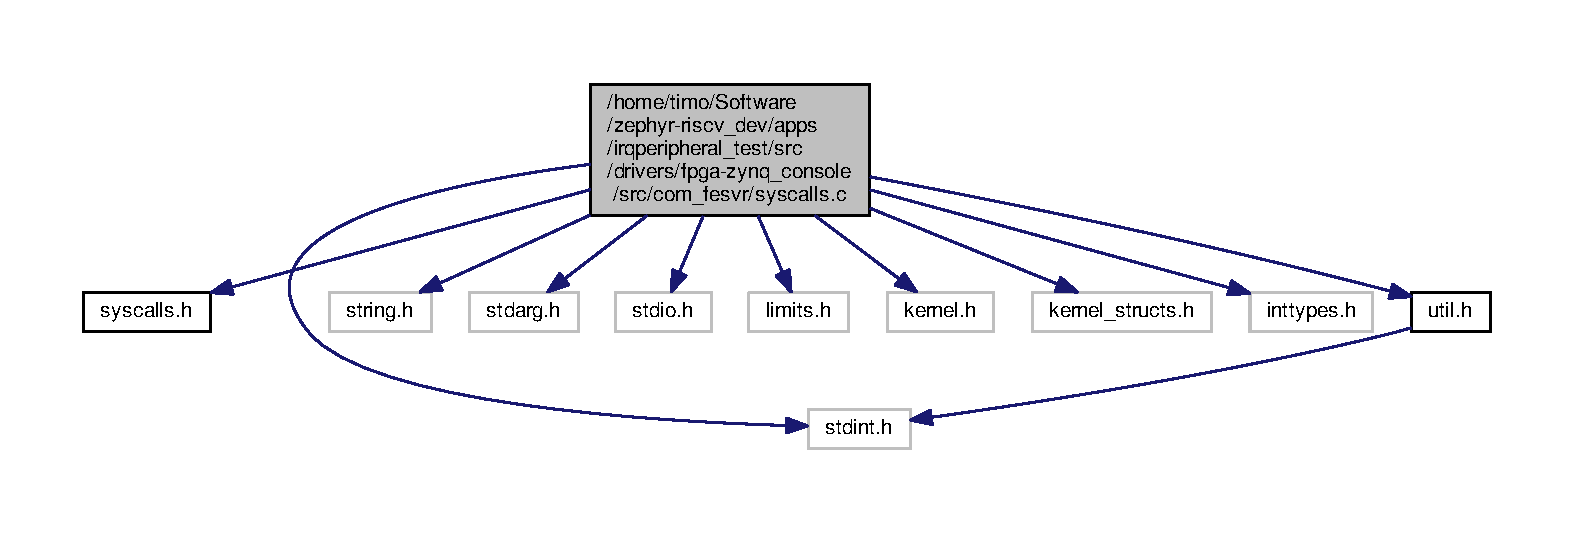
\includegraphics[width=350pt]{syscalls_8c__incl}
\end{center}
\end{figure}
\subsection*{Macros}
\begin{DoxyCompactItemize}
\item 
\#define \hyperlink{syscalls_8c_aa7425a6f80dc9c0ec789079cb6547542}{S\+Y\+S\+\_\+write}~64
\end{DoxyCompactItemize}
\subsection*{Functions}
\begin{DoxyCompactItemize}
\item 
static uintptr\+\_\+t \hyperlink{syscalls_8c_ae77bdb2f6ff0addff487d9829635999f}{syscall} (uintptr\+\_\+t which, uint64\+\_\+t arg0, uint64\+\_\+t arg1, uint64\+\_\+t arg2)
\item 
void \hyperlink{syscalls_8c_a93b9cf91f7623d6d8b100a3693d6d5e4}{\+\_\+\+\_\+attribute\+\_\+\+\_\+} ((noreturn))
\item 
uintptr\+\_\+t \hyperlink{syscalls_8c_aeb0fee7e25692380f5346f304f4b6e5a}{\+\_\+\+\_\+attribute\+\_\+\+\_\+} ((weak))
\item 
void \hyperlink{syscalls_8c_a7b17e5913b7dff48eec9ba3976ccfd3c}{exit} (int code)
\item 
void \hyperlink{syscalls_8c_ac54f53dc342019e8db34f4aa581a5792}{abort} ()
\item 
void \hyperlink{syscalls_8c_a2c232df4171975e520968ab9d6eea808}{printstr} (const char $\ast$s)
\item 
int \hyperlink{syscalls_8c_a96309354255db4e97ae7aea3a9874b91}{putchar\+\_\+2} (int ch)
\item 
void \hyperlink{syscalls_8c_a14dbeec7c4499cc6660a804cd69d2546}{printhex} (uint64\+\_\+t x)
\item 
static void \hyperlink{syscalls_8c_ad321bdb456d9be4ac65a8d5aba299be7}{printnum} (void($\ast$putch)(int, void $\ast$$\ast$), void $\ast$$\ast$putdat, unsigned long long num, unsigned base, int width, int padc)
\item 
static unsigned long long \hyperlink{syscalls_8c_a934736e8473edc7ac3a20c613ae5f732}{getuint} (va\+\_\+list $\ast$ap, int lflag)
\item 
static long long \hyperlink{syscalls_8c_a7b1e12e09f757ca234758afb4d704db8}{getint} (va\+\_\+list $\ast$ap, int lflag)
\item 
size\+\_\+t \hyperlink{syscalls_8c_a35dfa13e23fa51201d41c6bc3e20aae1}{strlen\+\_\+2} (const char $\ast$s)
\item 
size\+\_\+t \hyperlink{syscalls_8c_a7bd978e4981a80586c5b3a0dac22f0f2}{strnlen} (const char $\ast$s, size\+\_\+t n)
\item 
static void \hyperlink{syscalls_8c_a9dee5275dde68dd7e6546e93aa5ad639}{vprintfmt} (void($\ast$putch)(int, void $\ast$$\ast$), void $\ast$$\ast$putdat, const char $\ast$fmt, va\+\_\+list ap)
\item 
int \hyperlink{syscalls_8c_a37707a50cca88a28b765ce77ac1403e9}{printfsvr} (const char $\ast$fmt,...)
\end{DoxyCompactItemize}
\subsection*{Variables}
\begin{DoxyCompactItemize}
\item 
volatile uint64\+\_\+t \hyperlink{syscalls_8c_af4f0dc2fd18f5eccacc4ac0317972b29}{tohost}
\item 
volatile uint64\+\_\+t \hyperlink{syscalls_8c_a085cadbd59d5d173ab2621f7ebeedce3}{fromhost}
\end{DoxyCompactItemize}


\subsection{Macro Definition Documentation}
\index{syscalls.\+c@{syscalls.\+c}!S\+Y\+S\+\_\+write@{S\+Y\+S\+\_\+write}}
\index{S\+Y\+S\+\_\+write@{S\+Y\+S\+\_\+write}!syscalls.\+c@{syscalls.\+c}}
\subsubsection[{\texorpdfstring{S\+Y\+S\+\_\+write}{SYS_write}}]{\setlength{\rightskip}{0pt plus 5cm}\#define S\+Y\+S\+\_\+write~64}\hypertarget{syscalls_8c_aa7425a6f80dc9c0ec789079cb6547542}{}\label{syscalls_8c_aa7425a6f80dc9c0ec789079cb6547542}


\subsection{Function Documentation}
\index{syscalls.\+c@{syscalls.\+c}!\+\_\+\+\_\+attribute\+\_\+\+\_\+@{\+\_\+\+\_\+attribute\+\_\+\+\_\+}}
\index{\+\_\+\+\_\+attribute\+\_\+\+\_\+@{\+\_\+\+\_\+attribute\+\_\+\+\_\+}!syscalls.\+c@{syscalls.\+c}}
\subsubsection[{\texorpdfstring{\+\_\+\+\_\+attribute\+\_\+\+\_\+((noreturn))}{__attribute__((noreturn))}}]{\setlength{\rightskip}{0pt plus 5cm}void \+\_\+\+\_\+attribute\+\_\+\+\_\+ (
\begin{DoxyParamCaption}
\item[{(noreturn)}]{}
\end{DoxyParamCaption}
)}\hypertarget{syscalls_8c_a93b9cf91f7623d6d8b100a3693d6d5e4}{}\label{syscalls_8c_a93b9cf91f7623d6d8b100a3693d6d5e4}
\index{syscalls.\+c@{syscalls.\+c}!\+\_\+\+\_\+attribute\+\_\+\+\_\+@{\+\_\+\+\_\+attribute\+\_\+\+\_\+}}
\index{\+\_\+\+\_\+attribute\+\_\+\+\_\+@{\+\_\+\+\_\+attribute\+\_\+\+\_\+}!syscalls.\+c@{syscalls.\+c}}
\subsubsection[{\texorpdfstring{\+\_\+\+\_\+attribute\+\_\+\+\_\+((weak))}{__attribute__((weak))}}]{\setlength{\rightskip}{0pt plus 5cm}int \+\_\+\+\_\+attribute\+\_\+\+\_\+ (
\begin{DoxyParamCaption}
\item[{(weak)}]{}
\end{DoxyParamCaption}
)}\hypertarget{syscalls_8c_aeb0fee7e25692380f5346f304f4b6e5a}{}\label{syscalls_8c_aeb0fee7e25692380f5346f304f4b6e5a}
\index{syscalls.\+c@{syscalls.\+c}!abort@{abort}}
\index{abort@{abort}!syscalls.\+c@{syscalls.\+c}}
\subsubsection[{\texorpdfstring{abort()}{abort()}}]{\setlength{\rightskip}{0pt plus 5cm}void abort (
\begin{DoxyParamCaption}
{}
\end{DoxyParamCaption}
)}\hypertarget{syscalls_8c_ac54f53dc342019e8db34f4aa581a5792}{}\label{syscalls_8c_ac54f53dc342019e8db34f4aa581a5792}


Here is the call graph for this function\+:\nopagebreak
\begin{figure}[H]
\begin{center}
\leavevmode
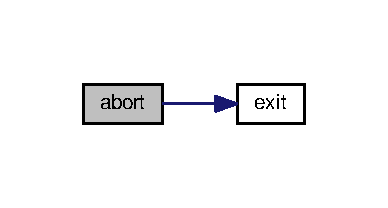
\includegraphics[width=186pt]{syscalls_8c_ac54f53dc342019e8db34f4aa581a5792_cgraph}
\end{center}
\end{figure}


\index{syscalls.\+c@{syscalls.\+c}!exit@{exit}}
\index{exit@{exit}!syscalls.\+c@{syscalls.\+c}}
\subsubsection[{\texorpdfstring{exit(int code)}{exit(int code)}}]{\setlength{\rightskip}{0pt plus 5cm}void exit (
\begin{DoxyParamCaption}
\item[{int}]{code}
\end{DoxyParamCaption}
)}\hypertarget{syscalls_8c_a7b17e5913b7dff48eec9ba3976ccfd3c}{}\label{syscalls_8c_a7b17e5913b7dff48eec9ba3976ccfd3c}
\index{syscalls.\+c@{syscalls.\+c}!getint@{getint}}
\index{getint@{getint}!syscalls.\+c@{syscalls.\+c}}
\subsubsection[{\texorpdfstring{getint(va\+\_\+list $\ast$ap, int lflag)}{getint(va_list *ap, int lflag)}}]{\setlength{\rightskip}{0pt plus 5cm}static long long getint (
\begin{DoxyParamCaption}
\item[{va\+\_\+list $\ast$}]{ap, }
\item[{int}]{lflag}
\end{DoxyParamCaption}
)\hspace{0.3cm}{\ttfamily [static]}}\hypertarget{syscalls_8c_a7b1e12e09f757ca234758afb4d704db8}{}\label{syscalls_8c_a7b1e12e09f757ca234758afb4d704db8}
\index{syscalls.\+c@{syscalls.\+c}!getuint@{getuint}}
\index{getuint@{getuint}!syscalls.\+c@{syscalls.\+c}}
\subsubsection[{\texorpdfstring{getuint(va\+\_\+list $\ast$ap, int lflag)}{getuint(va_list *ap, int lflag)}}]{\setlength{\rightskip}{0pt plus 5cm}static unsigned long long getuint (
\begin{DoxyParamCaption}
\item[{va\+\_\+list $\ast$}]{ap, }
\item[{int}]{lflag}
\end{DoxyParamCaption}
)\hspace{0.3cm}{\ttfamily [static]}}\hypertarget{syscalls_8c_a934736e8473edc7ac3a20c613ae5f732}{}\label{syscalls_8c_a934736e8473edc7ac3a20c613ae5f732}
\index{syscalls.\+c@{syscalls.\+c}!printfsvr@{printfsvr}}
\index{printfsvr@{printfsvr}!syscalls.\+c@{syscalls.\+c}}
\subsubsection[{\texorpdfstring{printfsvr(const char $\ast$fmt,...)}{printfsvr(const char *fmt,...)}}]{\setlength{\rightskip}{0pt plus 5cm}int printfsvr (
\begin{DoxyParamCaption}
\item[{const char $\ast$}]{fmt, }
\item[{}]{...}
\end{DoxyParamCaption}
)}\hypertarget{syscalls_8c_a37707a50cca88a28b765ce77ac1403e9}{}\label{syscalls_8c_a37707a50cca88a28b765ce77ac1403e9}


Here is the call graph for this function\+:\nopagebreak
\begin{figure}[H]
\begin{center}
\leavevmode
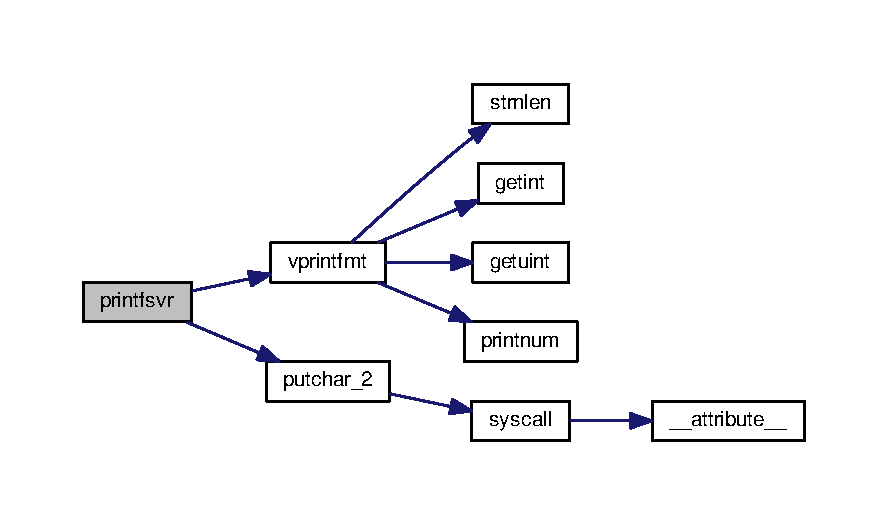
\includegraphics[width=350pt]{syscalls_8c_a37707a50cca88a28b765ce77ac1403e9_cgraph}
\end{center}
\end{figure}


\index{syscalls.\+c@{syscalls.\+c}!printhex@{printhex}}
\index{printhex@{printhex}!syscalls.\+c@{syscalls.\+c}}
\subsubsection[{\texorpdfstring{printhex(uint64\+\_\+t x)}{printhex(uint64_t x)}}]{\setlength{\rightskip}{0pt plus 5cm}void printhex (
\begin{DoxyParamCaption}
\item[{uint64\+\_\+t}]{x}
\end{DoxyParamCaption}
)}\hypertarget{syscalls_8c_a14dbeec7c4499cc6660a804cd69d2546}{}\label{syscalls_8c_a14dbeec7c4499cc6660a804cd69d2546}


Here is the call graph for this function\+:\nopagebreak
\begin{figure}[H]
\begin{center}
\leavevmode
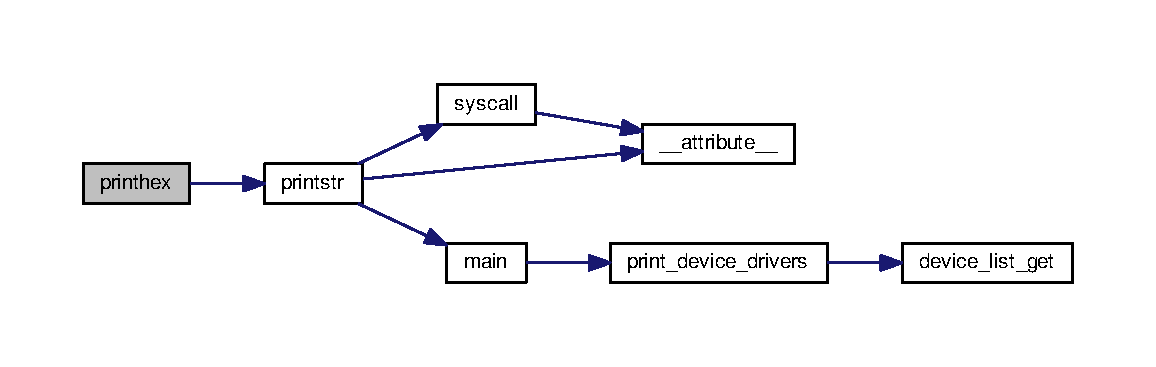
\includegraphics[width=350pt]{syscalls_8c_a14dbeec7c4499cc6660a804cd69d2546_cgraph}
\end{center}
\end{figure}


\index{syscalls.\+c@{syscalls.\+c}!printnum@{printnum}}
\index{printnum@{printnum}!syscalls.\+c@{syscalls.\+c}}
\subsubsection[{\texorpdfstring{printnum(void($\ast$putch)(int, void $\ast$$\ast$), void $\ast$$\ast$putdat, unsigned long long num, unsigned base, int width, int padc)}{printnum(void(*putch)(int, void **), void **putdat, unsigned long long num, unsigned base, int width, int padc)}}]{\setlength{\rightskip}{0pt plus 5cm}static void printnum (
\begin{DoxyParamCaption}
\item[{void($\ast$)(int, void $\ast$$\ast$)}]{putch, }
\item[{void $\ast$$\ast$}]{putdat, }
\item[{unsigned long long}]{num, }
\item[{unsigned}]{base, }
\item[{int}]{width, }
\item[{int}]{padc}
\end{DoxyParamCaption}
)\hspace{0.3cm}{\ttfamily [inline]}, {\ttfamily [static]}}\hypertarget{syscalls_8c_ad321bdb456d9be4ac65a8d5aba299be7}{}\label{syscalls_8c_ad321bdb456d9be4ac65a8d5aba299be7}
\index{syscalls.\+c@{syscalls.\+c}!printstr@{printstr}}
\index{printstr@{printstr}!syscalls.\+c@{syscalls.\+c}}
\subsubsection[{\texorpdfstring{printstr(const char $\ast$s)}{printstr(const char *s)}}]{\setlength{\rightskip}{0pt plus 5cm}void printstr (
\begin{DoxyParamCaption}
\item[{const char $\ast$}]{s}
\end{DoxyParamCaption}
)}\hypertarget{syscalls_8c_a2c232df4171975e520968ab9d6eea808}{}\label{syscalls_8c_a2c232df4171975e520968ab9d6eea808}


Here is the call graph for this function\+:\nopagebreak
\begin{figure}[H]
\begin{center}
\leavevmode
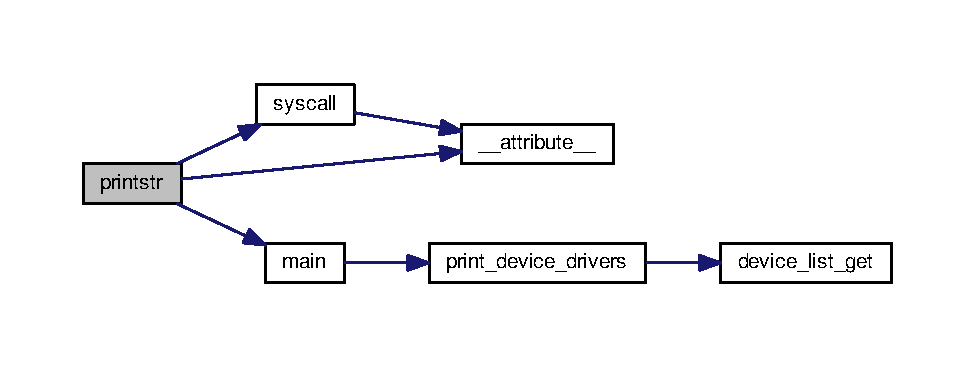
\includegraphics[width=350pt]{syscalls_8c_a2c232df4171975e520968ab9d6eea808_cgraph}
\end{center}
\end{figure}


\index{syscalls.\+c@{syscalls.\+c}!putchar\+\_\+2@{putchar\+\_\+2}}
\index{putchar\+\_\+2@{putchar\+\_\+2}!syscalls.\+c@{syscalls.\+c}}
\subsubsection[{\texorpdfstring{putchar\+\_\+2(int ch)}{putchar_2(int ch)}}]{\setlength{\rightskip}{0pt plus 5cm}int putchar\+\_\+2 (
\begin{DoxyParamCaption}
\item[{int}]{ch}
\end{DoxyParamCaption}
)}\hypertarget{syscalls_8c_a96309354255db4e97ae7aea3a9874b91}{}\label{syscalls_8c_a96309354255db4e97ae7aea3a9874b91}


Here is the call graph for this function\+:\nopagebreak
\begin{figure}[H]
\begin{center}
\leavevmode
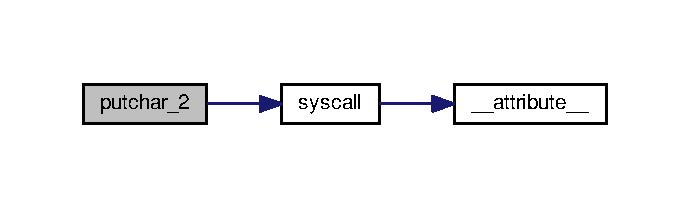
\includegraphics[width=331pt]{syscalls_8c_a96309354255db4e97ae7aea3a9874b91_cgraph}
\end{center}
\end{figure}


\index{syscalls.\+c@{syscalls.\+c}!strlen\+\_\+2@{strlen\+\_\+2}}
\index{strlen\+\_\+2@{strlen\+\_\+2}!syscalls.\+c@{syscalls.\+c}}
\subsubsection[{\texorpdfstring{strlen\+\_\+2(const char $\ast$s)}{strlen_2(const char *s)}}]{\setlength{\rightskip}{0pt plus 5cm}size\+\_\+t strlen\+\_\+2 (
\begin{DoxyParamCaption}
\item[{const char $\ast$}]{s}
\end{DoxyParamCaption}
)}\hypertarget{syscalls_8c_a35dfa13e23fa51201d41c6bc3e20aae1}{}\label{syscalls_8c_a35dfa13e23fa51201d41c6bc3e20aae1}
\index{syscalls.\+c@{syscalls.\+c}!strnlen@{strnlen}}
\index{strnlen@{strnlen}!syscalls.\+c@{syscalls.\+c}}
\subsubsection[{\texorpdfstring{strnlen(const char $\ast$s, size\+\_\+t n)}{strnlen(const char *s, size_t n)}}]{\setlength{\rightskip}{0pt plus 5cm}size\+\_\+t strnlen (
\begin{DoxyParamCaption}
\item[{const char $\ast$}]{s, }
\item[{size\+\_\+t}]{n}
\end{DoxyParamCaption}
)}\hypertarget{syscalls_8c_a7bd978e4981a80586c5b3a0dac22f0f2}{}\label{syscalls_8c_a7bd978e4981a80586c5b3a0dac22f0f2}
\index{syscalls.\+c@{syscalls.\+c}!syscall@{syscall}}
\index{syscall@{syscall}!syscalls.\+c@{syscalls.\+c}}
\subsubsection[{\texorpdfstring{syscall(uintptr\+\_\+t which, uint64\+\_\+t arg0, uint64\+\_\+t arg1, uint64\+\_\+t arg2)}{syscall(uintptr_t which, uint64_t arg0, uint64_t arg1, uint64_t arg2)}}]{\setlength{\rightskip}{0pt plus 5cm}static uintptr\+\_\+t syscall (
\begin{DoxyParamCaption}
\item[{uintptr\+\_\+t}]{which, }
\item[{uint64\+\_\+t}]{arg0, }
\item[{uint64\+\_\+t}]{arg1, }
\item[{uint64\+\_\+t}]{arg2}
\end{DoxyParamCaption}
)\hspace{0.3cm}{\ttfamily [static]}}\hypertarget{syscalls_8c_ae77bdb2f6ff0addff487d9829635999f}{}\label{syscalls_8c_ae77bdb2f6ff0addff487d9829635999f}


Here is the call graph for this function\+:\nopagebreak
\begin{figure}[H]
\begin{center}
\leavevmode
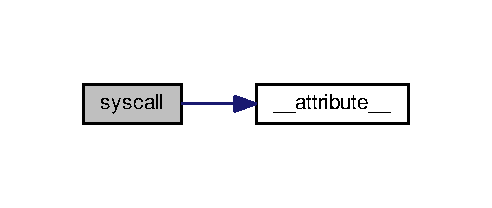
\includegraphics[width=236pt]{syscalls_8c_ae77bdb2f6ff0addff487d9829635999f_cgraph}
\end{center}
\end{figure}


\index{syscalls.\+c@{syscalls.\+c}!vprintfmt@{vprintfmt}}
\index{vprintfmt@{vprintfmt}!syscalls.\+c@{syscalls.\+c}}
\subsubsection[{\texorpdfstring{vprintfmt(void($\ast$putch)(int, void $\ast$$\ast$), void $\ast$$\ast$putdat, const char $\ast$fmt, va\+\_\+list ap)}{vprintfmt(void(*putch)(int, void **), void **putdat, const char *fmt, va_list ap)}}]{\setlength{\rightskip}{0pt plus 5cm}static void vprintfmt (
\begin{DoxyParamCaption}
\item[{void($\ast$)(int, void $\ast$$\ast$)}]{putch, }
\item[{void $\ast$$\ast$}]{putdat, }
\item[{const char $\ast$}]{fmt, }
\item[{va\+\_\+list}]{ap}
\end{DoxyParamCaption}
)\hspace{0.3cm}{\ttfamily [static]}}\hypertarget{syscalls_8c_a9dee5275dde68dd7e6546e93aa5ad639}{}\label{syscalls_8c_a9dee5275dde68dd7e6546e93aa5ad639}


Here is the call graph for this function\+:\nopagebreak
\begin{figure}[H]
\begin{center}
\leavevmode
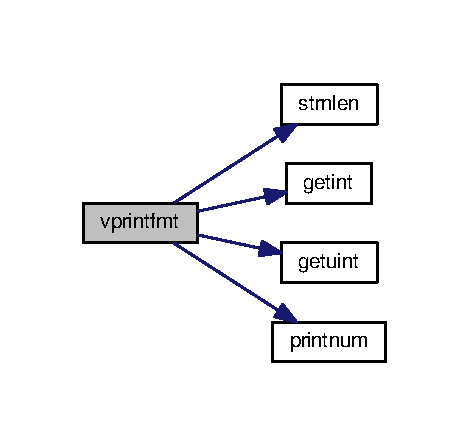
\includegraphics[width=225pt]{syscalls_8c_a9dee5275dde68dd7e6546e93aa5ad639_cgraph}
\end{center}
\end{figure}




\subsection{Variable Documentation}
\index{syscalls.\+c@{syscalls.\+c}!fromhost@{fromhost}}
\index{fromhost@{fromhost}!syscalls.\+c@{syscalls.\+c}}
\subsubsection[{\texorpdfstring{fromhost}{fromhost}}]{\setlength{\rightskip}{0pt plus 5cm}volatile uint64\+\_\+t fromhost}\hypertarget{syscalls_8c_a085cadbd59d5d173ab2621f7ebeedce3}{}\label{syscalls_8c_a085cadbd59d5d173ab2621f7ebeedce3}
\index{syscalls.\+c@{syscalls.\+c}!tohost@{tohost}}
\index{tohost@{tohost}!syscalls.\+c@{syscalls.\+c}}
\subsubsection[{\texorpdfstring{tohost}{tohost}}]{\setlength{\rightskip}{0pt plus 5cm}volatile uint64\+\_\+t tohost}\hypertarget{syscalls_8c_af4f0dc2fd18f5eccacc4ac0317972b29}{}\label{syscalls_8c_af4f0dc2fd18f5eccacc4ac0317972b29}

\hypertarget{syscalls_8h}{}\section{/home/timo/\+Software/zephyr-\/riscv\+\_\+dev/apps/irqperipheral\+\_\+test/src/drivers/fpga-\/zynq\+\_\+console/src/com\+\_\+fesvr/syscalls.h File Reference}
\label{syscalls_8h}\index{/home/timo/\+Software/zephyr-\/riscv\+\_\+dev/apps/irqperipheral\+\_\+test/src/drivers/fpga-\/zynq\+\_\+console/src/com\+\_\+fesvr/syscalls.\+h@{/home/timo/\+Software/zephyr-\/riscv\+\_\+dev/apps/irqperipheral\+\_\+test/src/drivers/fpga-\/zynq\+\_\+console/src/com\+\_\+fesvr/syscalls.\+h}}


Stripped down version from riscv-\/tools/riscv-\/tests/benchmark/common for printing to fesvr console.  


This graph shows which files directly or indirectly include this file\+:\nopagebreak
\begin{figure}[H]
\begin{center}
\leavevmode
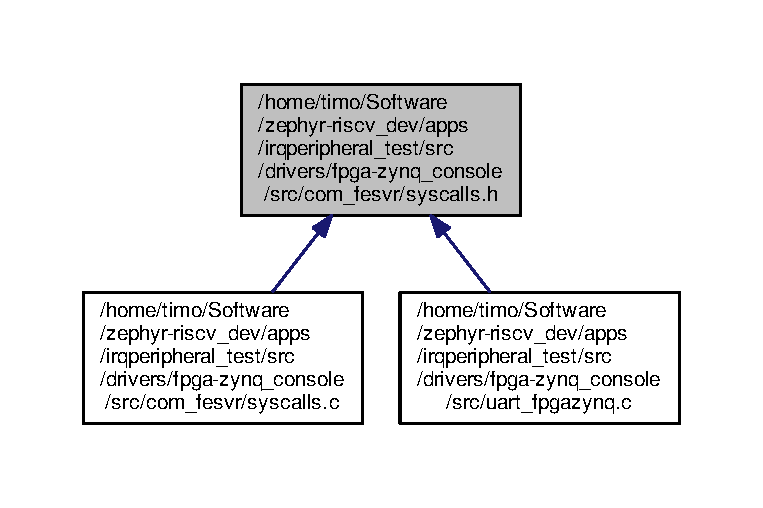
\includegraphics[width=350pt]{syscalls_8h__dep__incl}
\end{center}
\end{figure}
\subsection*{Functions}
\begin{DoxyCompactItemize}
\item 
int \hyperlink{syscalls_8h_a37707a50cca88a28b765ce77ac1403e9}{printfsvr} (const char $\ast$fmt,...)
\end{DoxyCompactItemize}


\subsection{Detailed Description}
Stripped down version from riscv-\/tools/riscv-\/tests/benchmark/common for printing to fesvr console. 



\subsection{Function Documentation}
\index{syscalls.\+h@{syscalls.\+h}!printfsvr@{printfsvr}}
\index{printfsvr@{printfsvr}!syscalls.\+h@{syscalls.\+h}}
\subsubsection[{\texorpdfstring{printfsvr(const char $\ast$fmt,...)}{printfsvr(const char *fmt,...)}}]{\setlength{\rightskip}{0pt plus 5cm}int printfsvr (
\begin{DoxyParamCaption}
\item[{const char $\ast$}]{fmt, }
\item[{}]{...}
\end{DoxyParamCaption}
)}\hypertarget{syscalls_8h_a37707a50cca88a28b765ce77ac1403e9}{}\label{syscalls_8h_a37707a50cca88a28b765ce77ac1403e9}


Here is the call graph for this function\+:\nopagebreak
\begin{figure}[H]
\begin{center}
\leavevmode
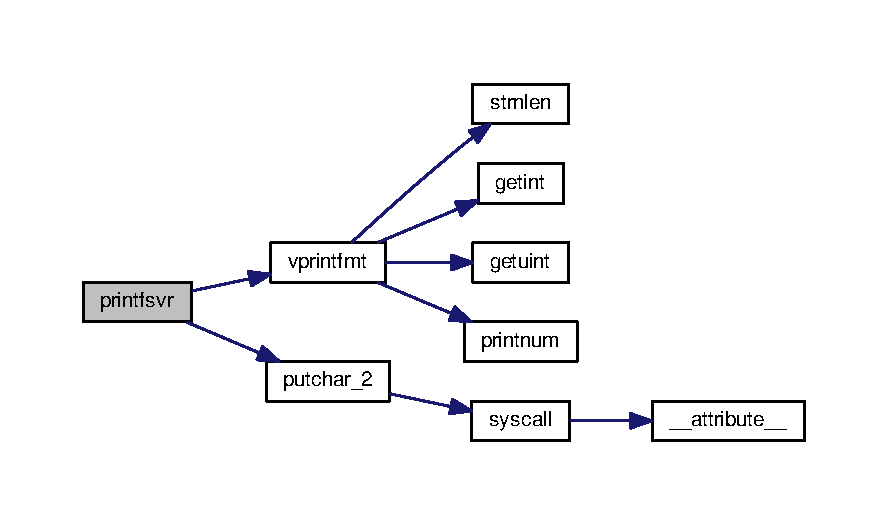
\includegraphics[width=350pt]{syscalls_8h_a37707a50cca88a28b765ce77ac1403e9_cgraph}
\end{center}
\end{figure}



\hypertarget{util_8h}{}\section{/home/timo/\+Software/zephyr-\/riscv\+\_\+dev/apps/irqperipheral\+\_\+test/src/drivers/fpga-\/zynq\+\_\+console/src/com\+\_\+fesvr/util.h File Reference}
\label{util_8h}\index{/home/timo/\+Software/zephyr-\/riscv\+\_\+dev/apps/irqperipheral\+\_\+test/src/drivers/fpga-\/zynq\+\_\+console/src/com\+\_\+fesvr/util.\+h@{/home/timo/\+Software/zephyr-\/riscv\+\_\+dev/apps/irqperipheral\+\_\+test/src/drivers/fpga-\/zynq\+\_\+console/src/com\+\_\+fesvr/util.\+h}}
{\ttfamily \#include $<$stdint.\+h$>$}\\*
Include dependency graph for util.\+h\+:\nopagebreak
\begin{figure}[H]
\begin{center}
\leavevmode
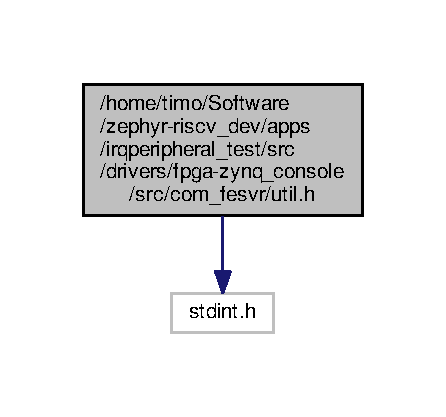
\includegraphics[width=214pt]{util_8h__incl}
\end{center}
\end{figure}
This graph shows which files directly or indirectly include this file\+:\nopagebreak
\begin{figure}[H]
\begin{center}
\leavevmode
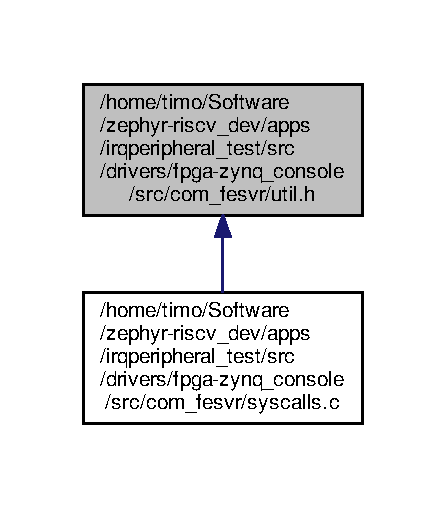
\includegraphics[width=214pt]{util_8h__dep__incl}
\end{center}
\end{figure}
\subsection*{Macros}
\begin{DoxyCompactItemize}
\item 
\#define \hyperlink{util_8h_ad072c9a7fa6508417f73e3e24943d89f}{static\+\_\+assert}(cond)~switch(0) \{ case 0\+: case !!(long)(cond)\+: ; \}
\item 
\#define \hyperlink{util_8h_ad3edcac6b9bfb0ad2ba9460be0c8d91b}{stringify\+\_\+1}(s)~\#s
\item 
\#define \hyperlink{util_8h_ad21edfbf3d91d1af380e8d842e35960f}{stringify}(s)~\hyperlink{util_8h_ad3edcac6b9bfb0ad2ba9460be0c8d91b}{stringify\+\_\+1}(s)
\item 
\#define \hyperlink{util_8h_aa2330e5664997c21b60a1aec2d1665ef}{stats}(code,  iter)
\end{DoxyCompactItemize}
\subsection*{Functions}
\begin{DoxyCompactItemize}
\item 
void \hyperlink{util_8h_a20f94d410fddf3860ae674314f91e75b}{set\+Stats} (int enable)
\end{DoxyCompactItemize}


\subsection{Macro Definition Documentation}
\index{util.\+h@{util.\+h}!static\+\_\+assert@{static\+\_\+assert}}
\index{static\+\_\+assert@{static\+\_\+assert}!util.\+h@{util.\+h}}
\subsubsection[{\texorpdfstring{static\+\_\+assert}{static_assert}}]{\setlength{\rightskip}{0pt plus 5cm}\#define static\+\_\+assert(
\begin{DoxyParamCaption}
\item[{}]{cond}
\end{DoxyParamCaption}
)~switch(0) \{ case 0\+: case !!(long)(cond)\+: ; \}}\hypertarget{util_8h_ad072c9a7fa6508417f73e3e24943d89f}{}\label{util_8h_ad072c9a7fa6508417f73e3e24943d89f}
\index{util.\+h@{util.\+h}!stats@{stats}}
\index{stats@{stats}!util.\+h@{util.\+h}}
\subsubsection[{\texorpdfstring{stats}{stats}}]{\setlength{\rightskip}{0pt plus 5cm}\#define stats(
\begin{DoxyParamCaption}
\item[{}]{code, }
\item[{}]{iter}
\end{DoxyParamCaption}
)}\hypertarget{util_8h_aa2330e5664997c21b60a1aec2d1665ef}{}\label{util_8h_aa2330e5664997c21b60a1aec2d1665ef}
{\bfseries Value\+:}
\begin{DoxyCode}
\textcolor{keywordflow}{do} \{ \(\backslash\)
    unsigned \textcolor{keywordtype}{long} \_c = -read\_csr(mcycle), \_i = -read\_csr(minstret); \(\backslash\)
    code; \(\backslash\)
    \_c += read\_csr(mcycle), \_i += read\_csr(minstret); \(\backslash\)
    if (cid == 0) \(\backslash\)
      printf(\textcolor{stringliteral}{"\(\backslash\)n%s: %ld cycles, %ld.%ld cycles/iter, %ld.%ld CPI\(\backslash\)n"}, \(\backslash\)
             \hyperlink{util_8h_ad21edfbf3d91d1af380e8d842e35960f}{stringify}(code), \_c, \_c/iter, 10*\_c/iter%10, \_c/\_i, 10*\_c/\_i%10); \(\backslash\)
  \} \textcolor{keywordflow}{while}(0)
\end{DoxyCode}
\index{util.\+h@{util.\+h}!stringify@{stringify}}
\index{stringify@{stringify}!util.\+h@{util.\+h}}
\subsubsection[{\texorpdfstring{stringify}{stringify}}]{\setlength{\rightskip}{0pt plus 5cm}\#define stringify(
\begin{DoxyParamCaption}
\item[{}]{s}
\end{DoxyParamCaption}
)~{\bf stringify\+\_\+1}(s)}\hypertarget{util_8h_ad21edfbf3d91d1af380e8d842e35960f}{}\label{util_8h_ad21edfbf3d91d1af380e8d842e35960f}
\index{util.\+h@{util.\+h}!stringify\+\_\+1@{stringify\+\_\+1}}
\index{stringify\+\_\+1@{stringify\+\_\+1}!util.\+h@{util.\+h}}
\subsubsection[{\texorpdfstring{stringify\+\_\+1}{stringify_1}}]{\setlength{\rightskip}{0pt plus 5cm}\#define stringify\+\_\+1(
\begin{DoxyParamCaption}
\item[{}]{s}
\end{DoxyParamCaption}
)~\#s}\hypertarget{util_8h_ad3edcac6b9bfb0ad2ba9460be0c8d91b}{}\label{util_8h_ad3edcac6b9bfb0ad2ba9460be0c8d91b}


\subsection{Function Documentation}
\index{util.\+h@{util.\+h}!set\+Stats@{set\+Stats}}
\index{set\+Stats@{set\+Stats}!util.\+h@{util.\+h}}
\subsubsection[{\texorpdfstring{set\+Stats(int enable)}{setStats(int enable)}}]{\setlength{\rightskip}{0pt plus 5cm}void set\+Stats (
\begin{DoxyParamCaption}
\item[{int}]{enable}
\end{DoxyParamCaption}
)}\hypertarget{util_8h_a20f94d410fddf3860ae674314f91e75b}{}\label{util_8h_a20f94d410fddf3860ae674314f91e75b}

\hypertarget{drivers_2fpga-zynq__console_2src_2main_8c}{}\section{/home/timo/\+Software/zephyr-\/riscv\+\_\+dev/apps/irqperipheral\+\_\+test/src/drivers/fpga-\/zynq\+\_\+console/src/main.c File Reference}
\label{drivers_2fpga-zynq__console_2src_2main_8c}\index{/home/timo/\+Software/zephyr-\/riscv\+\_\+dev/apps/irqperipheral\+\_\+test/src/drivers/fpga-\/zynq\+\_\+console/src/main.\+c@{/home/timo/\+Software/zephyr-\/riscv\+\_\+dev/apps/irqperipheral\+\_\+test/src/drivers/fpga-\/zynq\+\_\+console/src/main.\+c}}
{\ttfamily \#include $<$zephyr.\+h$>$}\\*
{\ttfamily \#include $<$misc/printk.\+h$>$}\\*
{\ttfamily \#include $<$device.\+h$>$}\\*
{\ttfamily \#include $<$string.\+h$>$}\\*
Include dependency graph for main.\+c\+:\nopagebreak
\begin{figure}[H]
\begin{center}
\leavevmode
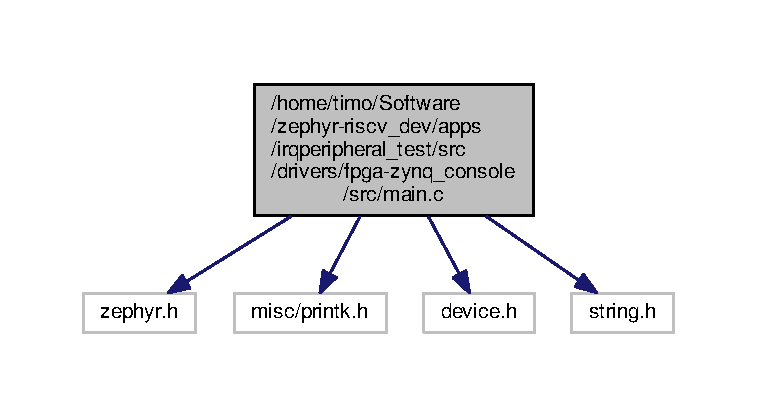
\includegraphics[width=350pt]{drivers_2fpga-zynq__console_2src_2main_8c__incl}
\end{center}
\end{figure}
\subsection*{Functions}
\begin{DoxyCompactItemize}
\item 
void \hyperlink{drivers_2fpga-zynq__console_2src_2main_8c_a42ee756b94eb5db2d5cd4d4c4bd73cee}{device\+\_\+list\+\_\+get} (struct device $\ast$$\ast$device\+\_\+list, int $\ast$device\+\_\+count)
\item 
void \hyperlink{drivers_2fpga-zynq__console_2src_2main_8c_addac945d30228d08bf924de4f324d15e}{print\+\_\+device\+\_\+drivers} ()
\item 
int \hyperlink{drivers_2fpga-zynq__console_2src_2main_8c_a840291bc02cba5474a4cb46a9b9566fe}{main} (void)
\end{DoxyCompactItemize}
\subsection*{Variables}
\begin{DoxyCompactItemize}
\item 
struct device \hyperlink{drivers_2fpga-zynq__console_2src_2main_8c_a3e123ce49c4fb9e881fba80d46192933}{\+\_\+\+\_\+device\+\_\+init\+\_\+end} \mbox{[}$\,$\mbox{]}
\item 
struct device \hyperlink{drivers_2fpga-zynq__console_2src_2main_8c_a287af280f14417dcbc1d27a65f12bc61}{\+\_\+\+\_\+device\+\_\+init\+\_\+start} \mbox{[}$\,$\mbox{]}
\end{DoxyCompactItemize}


\subsection{Function Documentation}
\index{drivers/fpga-\/zynq\+\_\+console/src/main.\+c@{drivers/fpga-\/zynq\+\_\+console/src/main.\+c}!device\+\_\+list\+\_\+get@{device\+\_\+list\+\_\+get}}
\index{device\+\_\+list\+\_\+get@{device\+\_\+list\+\_\+get}!drivers/fpga-\/zynq\+\_\+console/src/main.\+c@{drivers/fpga-\/zynq\+\_\+console/src/main.\+c}}
\subsubsection[{\texorpdfstring{device\+\_\+list\+\_\+get(struct device $\ast$$\ast$device\+\_\+list, int $\ast$device\+\_\+count)}{device_list_get(struct device **device_list, int *device_count)}}]{\setlength{\rightskip}{0pt plus 5cm}void device\+\_\+list\+\_\+get (
\begin{DoxyParamCaption}
\item[{struct device $\ast$$\ast$}]{device\+\_\+list, }
\item[{int $\ast$}]{device\+\_\+count}
\end{DoxyParamCaption}
)}\hypertarget{drivers_2fpga-zynq__console_2src_2main_8c_a42ee756b94eb5db2d5cd4d4c4bd73cee}{}\label{drivers_2fpga-zynq__console_2src_2main_8c_a42ee756b94eb5db2d5cd4d4c4bd73cee}
\index{drivers/fpga-\/zynq\+\_\+console/src/main.\+c@{drivers/fpga-\/zynq\+\_\+console/src/main.\+c}!main@{main}}
\index{main@{main}!drivers/fpga-\/zynq\+\_\+console/src/main.\+c@{drivers/fpga-\/zynq\+\_\+console/src/main.\+c}}
\subsubsection[{\texorpdfstring{main(void)}{main(void)}}]{\setlength{\rightskip}{0pt plus 5cm}int main (
\begin{DoxyParamCaption}
\item[{void}]{}
\end{DoxyParamCaption}
)}\hypertarget{drivers_2fpga-zynq__console_2src_2main_8c_a840291bc02cba5474a4cb46a9b9566fe}{}\label{drivers_2fpga-zynq__console_2src_2main_8c_a840291bc02cba5474a4cb46a9b9566fe}


Here is the call graph for this function\+:\nopagebreak
\begin{figure}[H]
\begin{center}
\leavevmode
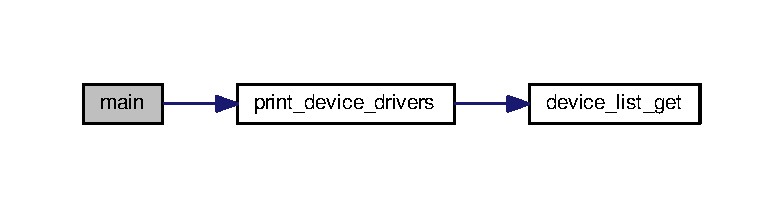
\includegraphics[width=350pt]{drivers_2fpga-zynq__console_2src_2main_8c_a840291bc02cba5474a4cb46a9b9566fe_cgraph}
\end{center}
\end{figure}


\index{drivers/fpga-\/zynq\+\_\+console/src/main.\+c@{drivers/fpga-\/zynq\+\_\+console/src/main.\+c}!print\+\_\+device\+\_\+drivers@{print\+\_\+device\+\_\+drivers}}
\index{print\+\_\+device\+\_\+drivers@{print\+\_\+device\+\_\+drivers}!drivers/fpga-\/zynq\+\_\+console/src/main.\+c@{drivers/fpga-\/zynq\+\_\+console/src/main.\+c}}
\subsubsection[{\texorpdfstring{print\+\_\+device\+\_\+drivers()}{print_device_drivers()}}]{\setlength{\rightskip}{0pt plus 5cm}void print\+\_\+device\+\_\+drivers (
\begin{DoxyParamCaption}
{}
\end{DoxyParamCaption}
)}\hypertarget{drivers_2fpga-zynq__console_2src_2main_8c_addac945d30228d08bf924de4f324d15e}{}\label{drivers_2fpga-zynq__console_2src_2main_8c_addac945d30228d08bf924de4f324d15e}


Here is the call graph for this function\+:\nopagebreak
\begin{figure}[H]
\begin{center}
\leavevmode
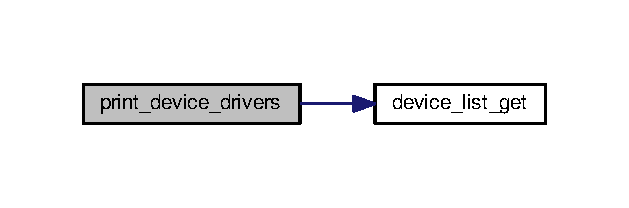
\includegraphics[width=302pt]{drivers_2fpga-zynq__console_2src_2main_8c_addac945d30228d08bf924de4f324d15e_cgraph}
\end{center}
\end{figure}




\subsection{Variable Documentation}
\index{drivers/fpga-\/zynq\+\_\+console/src/main.\+c@{drivers/fpga-\/zynq\+\_\+console/src/main.\+c}!\+\_\+\+\_\+device\+\_\+init\+\_\+end@{\+\_\+\+\_\+device\+\_\+init\+\_\+end}}
\index{\+\_\+\+\_\+device\+\_\+init\+\_\+end@{\+\_\+\+\_\+device\+\_\+init\+\_\+end}!drivers/fpga-\/zynq\+\_\+console/src/main.\+c@{drivers/fpga-\/zynq\+\_\+console/src/main.\+c}}
\subsubsection[{\texorpdfstring{\+\_\+\+\_\+device\+\_\+init\+\_\+end}{__device_init_end}}]{\setlength{\rightskip}{0pt plus 5cm}struct device \+\_\+\+\_\+device\+\_\+init\+\_\+end\mbox{[}$\,$\mbox{]}}\hypertarget{drivers_2fpga-zynq__console_2src_2main_8c_a3e123ce49c4fb9e881fba80d46192933}{}\label{drivers_2fpga-zynq__console_2src_2main_8c_a3e123ce49c4fb9e881fba80d46192933}
\index{drivers/fpga-\/zynq\+\_\+console/src/main.\+c@{drivers/fpga-\/zynq\+\_\+console/src/main.\+c}!\+\_\+\+\_\+device\+\_\+init\+\_\+start@{\+\_\+\+\_\+device\+\_\+init\+\_\+start}}
\index{\+\_\+\+\_\+device\+\_\+init\+\_\+start@{\+\_\+\+\_\+device\+\_\+init\+\_\+start}!drivers/fpga-\/zynq\+\_\+console/src/main.\+c@{drivers/fpga-\/zynq\+\_\+console/src/main.\+c}}
\subsubsection[{\texorpdfstring{\+\_\+\+\_\+device\+\_\+init\+\_\+start}{__device_init_start}}]{\setlength{\rightskip}{0pt plus 5cm}struct device \+\_\+\+\_\+device\+\_\+init\+\_\+start\mbox{[}$\,$\mbox{]}}\hypertarget{drivers_2fpga-zynq__console_2src_2main_8c_a287af280f14417dcbc1d27a65f12bc61}{}\label{drivers_2fpga-zynq__console_2src_2main_8c_a287af280f14417dcbc1d27a65f12bc61}

\hypertarget{main_8c}{}\section{/home/timo/\+Software/zephyr-\/riscv\+\_\+dev/apps/irqperipheral\+\_\+test/src/main.c File Reference}
\label{main_8c}\index{/home/timo/\+Software/zephyr-\/riscv\+\_\+dev/apps/irqperipheral\+\_\+test/src/main.\+c@{/home/timo/\+Software/zephyr-\/riscv\+\_\+dev/apps/irqperipheral\+\_\+test/src/main.\+c}}
{\ttfamily \#include $<$zephyr.\+h$>$}\\*
{\ttfamily \#include $<$misc/printk.\+h$>$}\\*
{\ttfamily \#include $<$device.\+h$>$}\\*
{\ttfamily \#include \char`\"{}globals.\+h\char`\"{}}\\*
{\ttfamily \#include \char`\"{}irqtestperipheral.\+h\char`\"{}}\\*
{\ttfamily \#include \char`\"{}tests/test\+\_\+runners.\+h\char`\"{}}\\*
{\ttfamily \#include \char`\"{}tests/tests.\+h\char`\"{}}\\*
{\ttfamily \#include \char`\"{}cycles.\+h\char`\"{}}\\*
{\ttfamily \#include \char`\"{}log\+\_\+perf.\+h\char`\"{}}\\*
{\ttfamily \#include \char`\"{}utils.\+h\char`\"{}}\\*
{\ttfamily \#include \char`\"{}state\+\_\+manager.\+h\char`\"{}}\\*
{\ttfamily \#include $<$string.\+h$>$}\\*
{\ttfamily \#include \char`\"{}state\+\_\+machines/sm1.\+h\char`\"{}}\\*
Include dependency graph for main.\+c\+:
\nopagebreak
\begin{figure}[H]
\begin{center}
\leavevmode
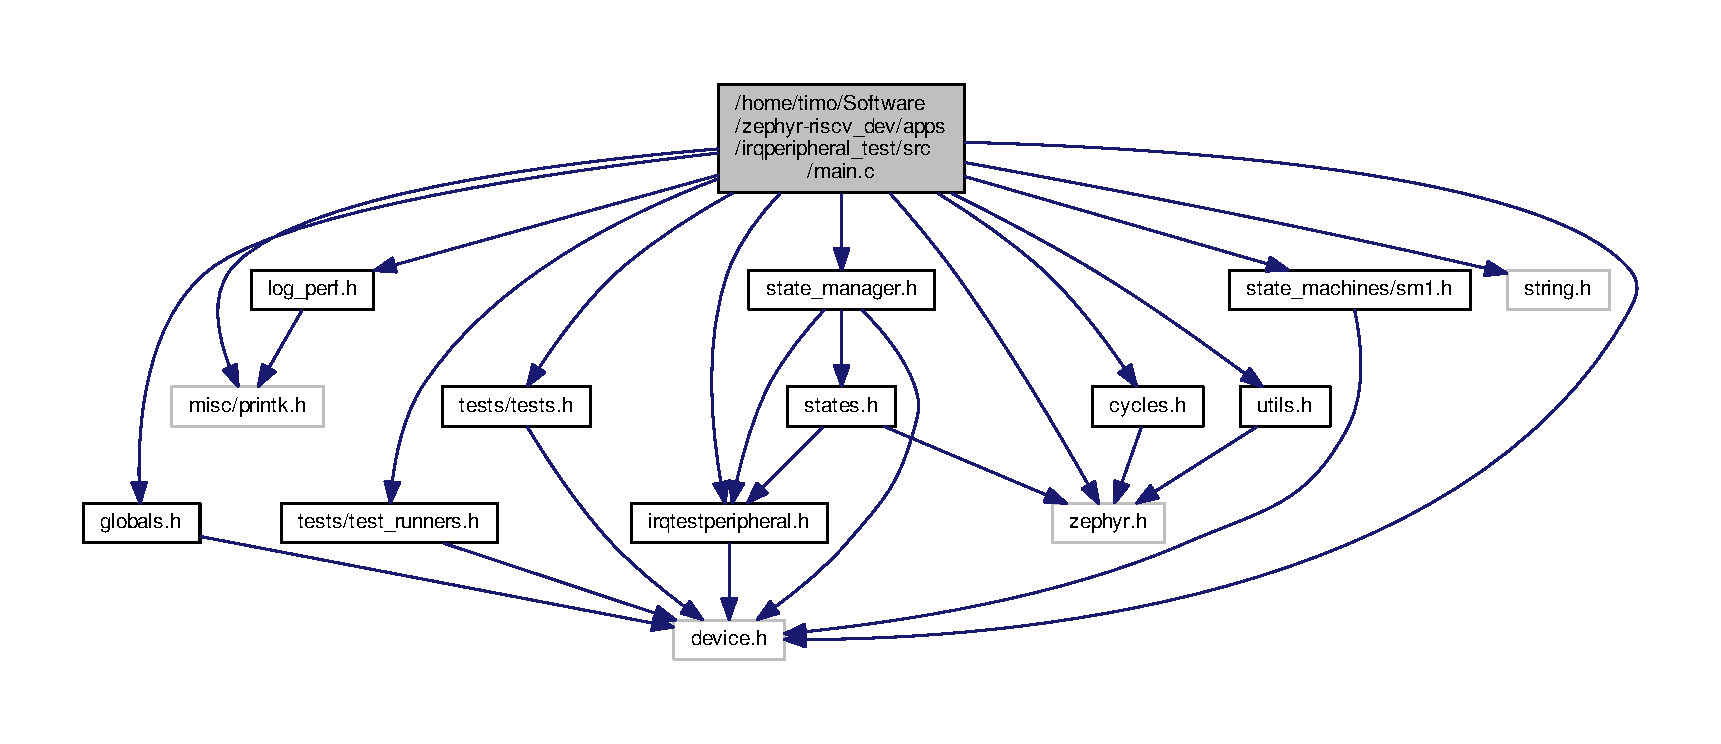
\includegraphics[width=350pt]{main_8c__incl}
\end{center}
\end{figure}
\subsection*{Macros}
\begin{DoxyCompactItemize}
\item 
\#define \hyperlink{main_8c_a419f922595dbc9aca2ef54b5f93589a1}{I\+R\+Q\+T\+E\+S\+T\+E\+R\+\_\+\+D\+R\+V\+\_\+\+N\+A\+ME}~\char`\"{}irqtester0\char`\"{}
\item 
\#define \hyperlink{main_8c_ad6830a9220bb2e0fb16a65c3b06faa5c}{U\+A\+R\+T1\+\_\+\+D\+R\+V\+\_\+\+N\+A\+ME}~\char`\"{}uart0\char`\"{}
\item 
\#define \hyperlink{main_8c_a3ac7f953c5a4ecb2a9f1b744d7067b0d}{U\+A\+R\+T2\+\_\+\+D\+R\+V\+\_\+\+N\+A\+ME}~\char`\"{}uart1\char`\"{}
\item 
\#define \hyperlink{main_8c_a3774232a16e17a4f482137e335c5d28b}{I\+R\+Q\+T\+E\+S\+T\+E\+R\+\_\+\+H\+W\+\_\+\+R\+EV}~3
\item 
\#define \hyperlink{main_8c_a355c43652842bcfa57fc2f00ed0da701}{P\+R\+I\+N\+T\+\_\+\+C\+O\+N\+F\+I\+G\+\_\+\+P\+R\+E\+E\+M\+P\+T\+\_\+\+E\+N\+A\+B\+L\+ED}~0
\item 
\#define \hyperlink{main_8c_a8d5c74db9f2b8d759bbffb1c5f08a1c6}{P\+R\+I\+N\+T\+\_\+\+C\+O\+N\+F\+I\+G\+\_\+\+T\+I\+M\+E\+S\+L\+I\+C\+I\+NG}~0
\item 
\#define \hyperlink{main_8c_a86a8c56755769823c3b901fbc06de384}{P\+R\+I\+N\+T\+\_\+\+C\+O\+N\+F\+I\+G\+\_\+\+I\+R\+Q\+\_\+\+O\+F\+F\+L\+O\+AD}~0
\end{DoxyCompactItemize}
\subsection*{Functions}
\begin{DoxyCompactItemize}
\item 
void \hyperlink{main_8c_a42ee756b94eb5db2d5cd4d4c4bd73cee}{device\+\_\+list\+\_\+get} (struct device $\ast$$\ast$device\+\_\+list, int $\ast$device\+\_\+count)
\item 
void \hyperlink{main_8c_addac945d30228d08bf924de4f324d15e}{print\+\_\+device\+\_\+drivers} ()
\item 
void \hyperlink{main_8c_ab108687134898bcfd0bd23956e74fe9d}{print\+\_\+kernel\+\_\+info} ()
\item 
void \hyperlink{main_8c_a7501a11f3b74b676df64fe525bae0ea3}{load\+\_\+drivers} ()
\item 
void \hyperlink{main_8c_a6288eba0f8e8ad3ab1544ad731eb7667}{main} (void)
\end{DoxyCompactItemize}
\subsection*{Variables}
\begin{DoxyCompactItemize}
\item 
int \hyperlink{main_8c_a19a71ebf8c414c631d6f29e7609e59cd}{global\+\_\+max\+\_\+cyc}
\item 
struct device \hyperlink{main_8c_a3e123ce49c4fb9e881fba80d46192933}{\+\_\+\+\_\+device\+\_\+init\+\_\+end} \mbox{[}$\,$\mbox{]}
\item 
struct device \hyperlink{main_8c_a287af280f14417dcbc1d27a65f12bc61}{\+\_\+\+\_\+device\+\_\+init\+\_\+start} \mbox{[}$\,$\mbox{]}
\item 
struct device $\ast$ \hyperlink{main_8c_abb59223368d7d7abf03bdd70c67d82a7}{g\+\_\+dev\+\_\+irqt}
\item 
struct device $\ast$ \hyperlink{main_8c_a4f93c31b6e082e5daf292aeac312ebf1}{g\+\_\+dev\+\_\+uart0}
\item 
struct device $\ast$ \hyperlink{main_8c_accc7e2dfa8f4bc5f10985ffa6aea9f78}{g\+\_\+dev\+\_\+uart1}
\end{DoxyCompactItemize}


\subsection{Macro Definition Documentation}
\index{main.\+c@{main.\+c}!I\+R\+Q\+T\+E\+S\+T\+E\+R\+\_\+\+D\+R\+V\+\_\+\+N\+A\+ME@{I\+R\+Q\+T\+E\+S\+T\+E\+R\+\_\+\+D\+R\+V\+\_\+\+N\+A\+ME}}
\index{I\+R\+Q\+T\+E\+S\+T\+E\+R\+\_\+\+D\+R\+V\+\_\+\+N\+A\+ME@{I\+R\+Q\+T\+E\+S\+T\+E\+R\+\_\+\+D\+R\+V\+\_\+\+N\+A\+ME}!main.\+c@{main.\+c}}
\subsubsection[{\texorpdfstring{I\+R\+Q\+T\+E\+S\+T\+E\+R\+\_\+\+D\+R\+V\+\_\+\+N\+A\+ME}{IRQTESTER_DRV_NAME}}]{\setlength{\rightskip}{0pt plus 5cm}\#define I\+R\+Q\+T\+E\+S\+T\+E\+R\+\_\+\+D\+R\+V\+\_\+\+N\+A\+ME~\char`\"{}irqtester0\char`\"{}}\hypertarget{main_8c_a419f922595dbc9aca2ef54b5f93589a1}{}\label{main_8c_a419f922595dbc9aca2ef54b5f93589a1}
\index{main.\+c@{main.\+c}!I\+R\+Q\+T\+E\+S\+T\+E\+R\+\_\+\+H\+W\+\_\+\+R\+EV@{I\+R\+Q\+T\+E\+S\+T\+E\+R\+\_\+\+H\+W\+\_\+\+R\+EV}}
\index{I\+R\+Q\+T\+E\+S\+T\+E\+R\+\_\+\+H\+W\+\_\+\+R\+EV@{I\+R\+Q\+T\+E\+S\+T\+E\+R\+\_\+\+H\+W\+\_\+\+R\+EV}!main.\+c@{main.\+c}}
\subsubsection[{\texorpdfstring{I\+R\+Q\+T\+E\+S\+T\+E\+R\+\_\+\+H\+W\+\_\+\+R\+EV}{IRQTESTER_HW_REV}}]{\setlength{\rightskip}{0pt plus 5cm}\#define I\+R\+Q\+T\+E\+S\+T\+E\+R\+\_\+\+H\+W\+\_\+\+R\+EV~3}\hypertarget{main_8c_a3774232a16e17a4f482137e335c5d28b}{}\label{main_8c_a3774232a16e17a4f482137e335c5d28b}
\index{main.\+c@{main.\+c}!P\+R\+I\+N\+T\+\_\+\+C\+O\+N\+F\+I\+G\+\_\+\+I\+R\+Q\+\_\+\+O\+F\+F\+L\+O\+AD@{P\+R\+I\+N\+T\+\_\+\+C\+O\+N\+F\+I\+G\+\_\+\+I\+R\+Q\+\_\+\+O\+F\+F\+L\+O\+AD}}
\index{P\+R\+I\+N\+T\+\_\+\+C\+O\+N\+F\+I\+G\+\_\+\+I\+R\+Q\+\_\+\+O\+F\+F\+L\+O\+AD@{P\+R\+I\+N\+T\+\_\+\+C\+O\+N\+F\+I\+G\+\_\+\+I\+R\+Q\+\_\+\+O\+F\+F\+L\+O\+AD}!main.\+c@{main.\+c}}
\subsubsection[{\texorpdfstring{P\+R\+I\+N\+T\+\_\+\+C\+O\+N\+F\+I\+G\+\_\+\+I\+R\+Q\+\_\+\+O\+F\+F\+L\+O\+AD}{PRINT_CONFIG_IRQ_OFFLOAD}}]{\setlength{\rightskip}{0pt plus 5cm}\#define P\+R\+I\+N\+T\+\_\+\+C\+O\+N\+F\+I\+G\+\_\+\+I\+R\+Q\+\_\+\+O\+F\+F\+L\+O\+AD~0}\hypertarget{main_8c_a86a8c56755769823c3b901fbc06de384}{}\label{main_8c_a86a8c56755769823c3b901fbc06de384}
\index{main.\+c@{main.\+c}!P\+R\+I\+N\+T\+\_\+\+C\+O\+N\+F\+I\+G\+\_\+\+P\+R\+E\+E\+M\+P\+T\+\_\+\+E\+N\+A\+B\+L\+ED@{P\+R\+I\+N\+T\+\_\+\+C\+O\+N\+F\+I\+G\+\_\+\+P\+R\+E\+E\+M\+P\+T\+\_\+\+E\+N\+A\+B\+L\+ED}}
\index{P\+R\+I\+N\+T\+\_\+\+C\+O\+N\+F\+I\+G\+\_\+\+P\+R\+E\+E\+M\+P\+T\+\_\+\+E\+N\+A\+B\+L\+ED@{P\+R\+I\+N\+T\+\_\+\+C\+O\+N\+F\+I\+G\+\_\+\+P\+R\+E\+E\+M\+P\+T\+\_\+\+E\+N\+A\+B\+L\+ED}!main.\+c@{main.\+c}}
\subsubsection[{\texorpdfstring{P\+R\+I\+N\+T\+\_\+\+C\+O\+N\+F\+I\+G\+\_\+\+P\+R\+E\+E\+M\+P\+T\+\_\+\+E\+N\+A\+B\+L\+ED}{PRINT_CONFIG_PREEMPT_ENABLED}}]{\setlength{\rightskip}{0pt plus 5cm}\#define P\+R\+I\+N\+T\+\_\+\+C\+O\+N\+F\+I\+G\+\_\+\+P\+R\+E\+E\+M\+P\+T\+\_\+\+E\+N\+A\+B\+L\+ED~0}\hypertarget{main_8c_a355c43652842bcfa57fc2f00ed0da701}{}\label{main_8c_a355c43652842bcfa57fc2f00ed0da701}
\index{main.\+c@{main.\+c}!P\+R\+I\+N\+T\+\_\+\+C\+O\+N\+F\+I\+G\+\_\+\+T\+I\+M\+E\+S\+L\+I\+C\+I\+NG@{P\+R\+I\+N\+T\+\_\+\+C\+O\+N\+F\+I\+G\+\_\+\+T\+I\+M\+E\+S\+L\+I\+C\+I\+NG}}
\index{P\+R\+I\+N\+T\+\_\+\+C\+O\+N\+F\+I\+G\+\_\+\+T\+I\+M\+E\+S\+L\+I\+C\+I\+NG@{P\+R\+I\+N\+T\+\_\+\+C\+O\+N\+F\+I\+G\+\_\+\+T\+I\+M\+E\+S\+L\+I\+C\+I\+NG}!main.\+c@{main.\+c}}
\subsubsection[{\texorpdfstring{P\+R\+I\+N\+T\+\_\+\+C\+O\+N\+F\+I\+G\+\_\+\+T\+I\+M\+E\+S\+L\+I\+C\+I\+NG}{PRINT_CONFIG_TIMESLICING}}]{\setlength{\rightskip}{0pt plus 5cm}\#define P\+R\+I\+N\+T\+\_\+\+C\+O\+N\+F\+I\+G\+\_\+\+T\+I\+M\+E\+S\+L\+I\+C\+I\+NG~0}\hypertarget{main_8c_a8d5c74db9f2b8d759bbffb1c5f08a1c6}{}\label{main_8c_a8d5c74db9f2b8d759bbffb1c5f08a1c6}
\index{main.\+c@{main.\+c}!U\+A\+R\+T1\+\_\+\+D\+R\+V\+\_\+\+N\+A\+ME@{U\+A\+R\+T1\+\_\+\+D\+R\+V\+\_\+\+N\+A\+ME}}
\index{U\+A\+R\+T1\+\_\+\+D\+R\+V\+\_\+\+N\+A\+ME@{U\+A\+R\+T1\+\_\+\+D\+R\+V\+\_\+\+N\+A\+ME}!main.\+c@{main.\+c}}
\subsubsection[{\texorpdfstring{U\+A\+R\+T1\+\_\+\+D\+R\+V\+\_\+\+N\+A\+ME}{UART1_DRV_NAME}}]{\setlength{\rightskip}{0pt plus 5cm}\#define U\+A\+R\+T1\+\_\+\+D\+R\+V\+\_\+\+N\+A\+ME~\char`\"{}uart0\char`\"{}}\hypertarget{main_8c_ad6830a9220bb2e0fb16a65c3b06faa5c}{}\label{main_8c_ad6830a9220bb2e0fb16a65c3b06faa5c}
\index{main.\+c@{main.\+c}!U\+A\+R\+T2\+\_\+\+D\+R\+V\+\_\+\+N\+A\+ME@{U\+A\+R\+T2\+\_\+\+D\+R\+V\+\_\+\+N\+A\+ME}}
\index{U\+A\+R\+T2\+\_\+\+D\+R\+V\+\_\+\+N\+A\+ME@{U\+A\+R\+T2\+\_\+\+D\+R\+V\+\_\+\+N\+A\+ME}!main.\+c@{main.\+c}}
\subsubsection[{\texorpdfstring{U\+A\+R\+T2\+\_\+\+D\+R\+V\+\_\+\+N\+A\+ME}{UART2_DRV_NAME}}]{\setlength{\rightskip}{0pt plus 5cm}\#define U\+A\+R\+T2\+\_\+\+D\+R\+V\+\_\+\+N\+A\+ME~\char`\"{}uart1\char`\"{}}\hypertarget{main_8c_a3ac7f953c5a4ecb2a9f1b744d7067b0d}{}\label{main_8c_a3ac7f953c5a4ecb2a9f1b744d7067b0d}


\subsection{Function Documentation}
\index{main.\+c@{main.\+c}!device\+\_\+list\+\_\+get@{device\+\_\+list\+\_\+get}}
\index{device\+\_\+list\+\_\+get@{device\+\_\+list\+\_\+get}!main.\+c@{main.\+c}}
\subsubsection[{\texorpdfstring{device\+\_\+list\+\_\+get(struct device $\ast$$\ast$device\+\_\+list, int $\ast$device\+\_\+count)}{device_list_get(struct device **device_list, int *device_count)}}]{\setlength{\rightskip}{0pt plus 5cm}void device\+\_\+list\+\_\+get (
\begin{DoxyParamCaption}
\item[{struct device $\ast$$\ast$}]{device\+\_\+list, }
\item[{int $\ast$}]{device\+\_\+count}
\end{DoxyParamCaption}
)}\hypertarget{main_8c_a42ee756b94eb5db2d5cd4d4c4bd73cee}{}\label{main_8c_a42ee756b94eb5db2d5cd4d4c4bd73cee}
\index{main.\+c@{main.\+c}!load\+\_\+drivers@{load\+\_\+drivers}}
\index{load\+\_\+drivers@{load\+\_\+drivers}!main.\+c@{main.\+c}}
\subsubsection[{\texorpdfstring{load\+\_\+drivers()}{load_drivers()}}]{\setlength{\rightskip}{0pt plus 5cm}void load\+\_\+drivers (
\begin{DoxyParamCaption}
{}
\end{DoxyParamCaption}
)}\hypertarget{main_8c_a7501a11f3b74b676df64fe525bae0ea3}{}\label{main_8c_a7501a11f3b74b676df64fe525bae0ea3}
\index{main.\+c@{main.\+c}!main@{main}}
\index{main@{main}!main.\+c@{main.\+c}}
\subsubsection[{\texorpdfstring{main(void)}{main(void)}}]{\setlength{\rightskip}{0pt plus 5cm}void main (
\begin{DoxyParamCaption}
\item[{void}]{}
\end{DoxyParamCaption}
)}\hypertarget{main_8c_a6288eba0f8e8ad3ab1544ad731eb7667}{}\label{main_8c_a6288eba0f8e8ad3ab1544ad731eb7667}
Printing policy a) logging (S\+Y\+S\+\_\+\+L\+O\+G\+\_\+$<$$>$) stuff that should vanish in time-\/critical builds -\/$>$ can be thrown out of code by Kconfig/logging b) (verbsoity controlled) printkv stuff in tests that is not time critical -\/$>$ can control via print\+\_\+set\+\_\+verbosity -\/$>$ stays in binary, even when vebosity set to not show -\/$>$ productive code should avoid compiling test code anyway c) buffered L\+O\+G\+\_\+\+P\+E\+RF stuff inside time-\/critical code that needs to be printed for debug -\/$>$ logs to buffer and prints after run -\/$>$ still slower than not printing, better than serial out -\/$>$ set C\+O\+N\+F\+I\+G\+\_\+\+A\+P\+P\+\_\+\+L\+O\+G\+\_\+\+P\+E\+R\+F\+\_\+\+B\+U\+F\+F\+E\+R\+\_\+\+D\+E\+P\+TH=0 to deactivate

Here is the call graph for this function\+:
\nopagebreak
\begin{figure}[H]
\begin{center}
\leavevmode
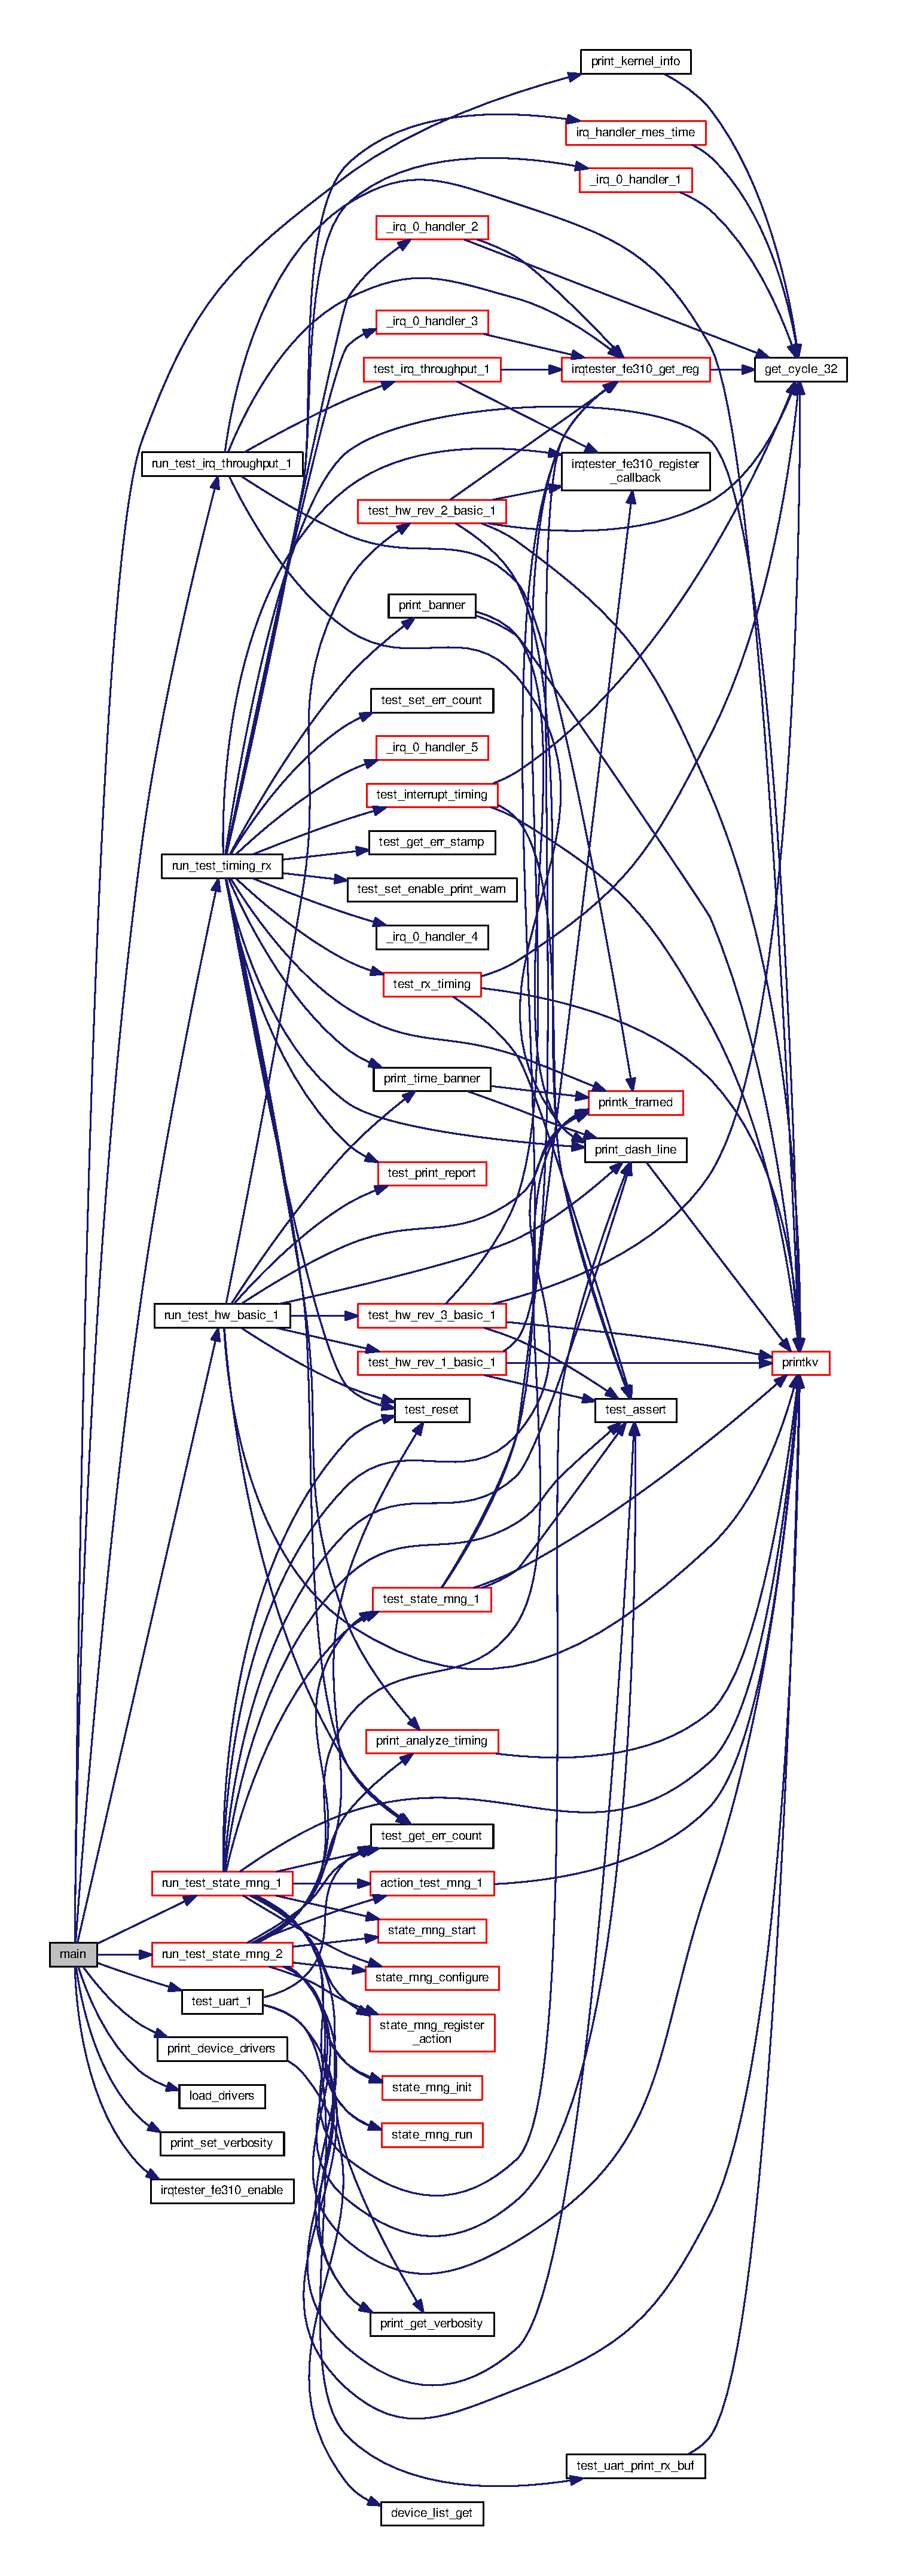
\includegraphics[height=550pt]{main_8c_a6288eba0f8e8ad3ab1544ad731eb7667_cgraph}
\end{center}
\end{figure}


\index{main.\+c@{main.\+c}!print\+\_\+device\+\_\+drivers@{print\+\_\+device\+\_\+drivers}}
\index{print\+\_\+device\+\_\+drivers@{print\+\_\+device\+\_\+drivers}!main.\+c@{main.\+c}}
\subsubsection[{\texorpdfstring{print\+\_\+device\+\_\+drivers()}{print_device_drivers()}}]{\setlength{\rightskip}{0pt plus 5cm}void print\+\_\+device\+\_\+drivers (
\begin{DoxyParamCaption}
{}
\end{DoxyParamCaption}
)}\hypertarget{main_8c_addac945d30228d08bf924de4f324d15e}{}\label{main_8c_addac945d30228d08bf924de4f324d15e}


Here is the call graph for this function\+:\nopagebreak
\begin{figure}[H]
\begin{center}
\leavevmode
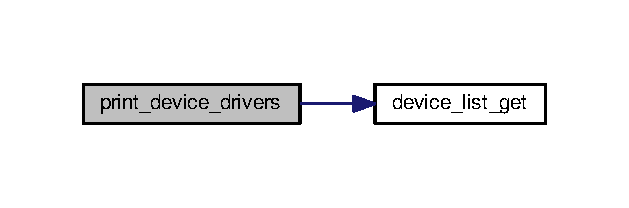
\includegraphics[width=302pt]{main_8c_addac945d30228d08bf924de4f324d15e_cgraph}
\end{center}
\end{figure}


\index{main.\+c@{main.\+c}!print\+\_\+kernel\+\_\+info@{print\+\_\+kernel\+\_\+info}}
\index{print\+\_\+kernel\+\_\+info@{print\+\_\+kernel\+\_\+info}!main.\+c@{main.\+c}}
\subsubsection[{\texorpdfstring{print\+\_\+kernel\+\_\+info()}{print_kernel_info()}}]{\setlength{\rightskip}{0pt plus 5cm}void print\+\_\+kernel\+\_\+info (
\begin{DoxyParamCaption}
{}
\end{DoxyParamCaption}
)}\hypertarget{main_8c_ab108687134898bcfd0bd23956e74fe9d}{}\label{main_8c_ab108687134898bcfd0bd23956e74fe9d}


Here is the call graph for this function\+:\nopagebreak
\begin{figure}[H]
\begin{center}
\leavevmode
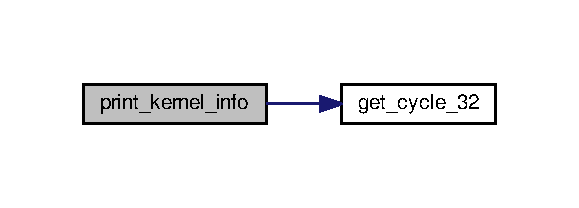
\includegraphics[width=278pt]{main_8c_ab108687134898bcfd0bd23956e74fe9d_cgraph}
\end{center}
\end{figure}




\subsection{Variable Documentation}
\index{main.\+c@{main.\+c}!\+\_\+\+\_\+device\+\_\+init\+\_\+end@{\+\_\+\+\_\+device\+\_\+init\+\_\+end}}
\index{\+\_\+\+\_\+device\+\_\+init\+\_\+end@{\+\_\+\+\_\+device\+\_\+init\+\_\+end}!main.\+c@{main.\+c}}
\subsubsection[{\texorpdfstring{\+\_\+\+\_\+device\+\_\+init\+\_\+end}{__device_init_end}}]{\setlength{\rightskip}{0pt plus 5cm}struct device \+\_\+\+\_\+device\+\_\+init\+\_\+end\mbox{[}$\,$\mbox{]}}\hypertarget{main_8c_a3e123ce49c4fb9e881fba80d46192933}{}\label{main_8c_a3e123ce49c4fb9e881fba80d46192933}
\index{main.\+c@{main.\+c}!\+\_\+\+\_\+device\+\_\+init\+\_\+start@{\+\_\+\+\_\+device\+\_\+init\+\_\+start}}
\index{\+\_\+\+\_\+device\+\_\+init\+\_\+start@{\+\_\+\+\_\+device\+\_\+init\+\_\+start}!main.\+c@{main.\+c}}
\subsubsection[{\texorpdfstring{\+\_\+\+\_\+device\+\_\+init\+\_\+start}{__device_init_start}}]{\setlength{\rightskip}{0pt plus 5cm}struct device \+\_\+\+\_\+device\+\_\+init\+\_\+start\mbox{[}$\,$\mbox{]}}\hypertarget{main_8c_a287af280f14417dcbc1d27a65f12bc61}{}\label{main_8c_a287af280f14417dcbc1d27a65f12bc61}
\index{main.\+c@{main.\+c}!g\+\_\+dev\+\_\+irqt@{g\+\_\+dev\+\_\+irqt}}
\index{g\+\_\+dev\+\_\+irqt@{g\+\_\+dev\+\_\+irqt}!main.\+c@{main.\+c}}
\subsubsection[{\texorpdfstring{g\+\_\+dev\+\_\+irqt}{g_dev_irqt}}]{\setlength{\rightskip}{0pt plus 5cm}struct device$\ast$ g\+\_\+dev\+\_\+irqt}\hypertarget{main_8c_abb59223368d7d7abf03bdd70c67d82a7}{}\label{main_8c_abb59223368d7d7abf03bdd70c67d82a7}
\index{main.\+c@{main.\+c}!g\+\_\+dev\+\_\+uart0@{g\+\_\+dev\+\_\+uart0}}
\index{g\+\_\+dev\+\_\+uart0@{g\+\_\+dev\+\_\+uart0}!main.\+c@{main.\+c}}
\subsubsection[{\texorpdfstring{g\+\_\+dev\+\_\+uart0}{g_dev_uart0}}]{\setlength{\rightskip}{0pt plus 5cm}struct device$\ast$ g\+\_\+dev\+\_\+uart0}\hypertarget{main_8c_a4f93c31b6e082e5daf292aeac312ebf1}{}\label{main_8c_a4f93c31b6e082e5daf292aeac312ebf1}
\index{main.\+c@{main.\+c}!g\+\_\+dev\+\_\+uart1@{g\+\_\+dev\+\_\+uart1}}
\index{g\+\_\+dev\+\_\+uart1@{g\+\_\+dev\+\_\+uart1}!main.\+c@{main.\+c}}
\subsubsection[{\texorpdfstring{g\+\_\+dev\+\_\+uart1}{g_dev_uart1}}]{\setlength{\rightskip}{0pt plus 5cm}struct device$\ast$ g\+\_\+dev\+\_\+uart1}\hypertarget{main_8c_accc7e2dfa8f4bc5f10985ffa6aea9f78}{}\label{main_8c_accc7e2dfa8f4bc5f10985ffa6aea9f78}
\index{main.\+c@{main.\+c}!global\+\_\+max\+\_\+cyc@{global\+\_\+max\+\_\+cyc}}
\index{global\+\_\+max\+\_\+cyc@{global\+\_\+max\+\_\+cyc}!main.\+c@{main.\+c}}
\subsubsection[{\texorpdfstring{global\+\_\+max\+\_\+cyc}{global_max_cyc}}]{\setlength{\rightskip}{0pt plus 5cm}int global\+\_\+max\+\_\+cyc}\hypertarget{main_8c_a19a71ebf8c414c631d6f29e7609e59cd}{}\label{main_8c_a19a71ebf8c414c631d6f29e7609e59cd}

\hypertarget{uart__fpgazynq_8c}{}\section{/home/timo/\+Software/zephyr-\/riscv\+\_\+dev/apps/irqperipheral\+\_\+test/src/drivers/fpga-\/zynq\+\_\+console/src/uart\+\_\+fpgazynq.c File Reference}
\label{uart__fpgazynq_8c}\index{/home/timo/\+Software/zephyr-\/riscv\+\_\+dev/apps/irqperipheral\+\_\+test/src/drivers/fpga-\/zynq\+\_\+console/src/uart\+\_\+fpgazynq.\+c@{/home/timo/\+Software/zephyr-\/riscv\+\_\+dev/apps/irqperipheral\+\_\+test/src/drivers/fpga-\/zynq\+\_\+console/src/uart\+\_\+fpgazynq.\+c}}


Driver for console output to fpga-\/zynq\textquotesingle{}s frontend server (fesvr)  


{\ttfamily \#include $<$kernel.\+h$>$}\\*
{\ttfamily \#include $<$arch/cpu.\+h$>$}\\*
{\ttfamily \#include $<$uart.\+h$>$}\\*
{\ttfamily \#include $<$board.\+h$>$}\\*
{\ttfamily \#include \char`\"{}com\+\_\+fesvr/syscalls.\+h\char`\"{}}\\*
Include dependency graph for uart\+\_\+fpgazynq.\+c\+:\nopagebreak
\begin{figure}[H]
\begin{center}
\leavevmode
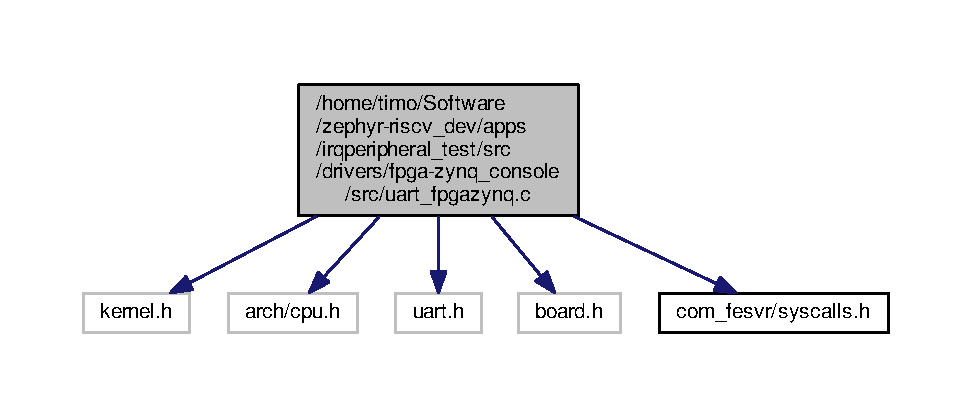
\includegraphics[width=350pt]{uart__fpgazynq_8c__incl}
\end{center}
\end{figure}
\subsection*{Data Structures}
\begin{DoxyCompactItemize}
\item 
struct \hyperlink{structuart__fpgazynq__device__config}{uart\+\_\+fpgazynq\+\_\+device\+\_\+config}
\item 
struct \hyperlink{structuart__fpgazynq__data}{uart\+\_\+fpgazynq\+\_\+data}
\end{DoxyCompactItemize}
\subsection*{Macros}
\begin{DoxyCompactItemize}
\item 
\#define \hyperlink{uart__fpgazynq_8c_ab5c3864067257693d9bef98c3fe8fc2b}{D\+E\+V\+\_\+\+C\+FG}(dev)
\item 
\#define \hyperlink{uart__fpgazynq_8c_aa90b045b0cf3a7fe70c69ba16eb135cc}{D\+E\+V\+\_\+\+D\+A\+TA}(dev)~((struct \hyperlink{structuart__fpgazynq__data}{uart\+\_\+fpgazynq\+\_\+data} $\ast$ const)(dev)-\/$>$driver\+\_\+data)
\end{DoxyCompactItemize}
\subsection*{Functions}
\begin{DoxyCompactItemize}
\item 
static unsigned char \hyperlink{uart__fpgazynq_8c_a851bc4f05ccf668befa650b3ac66b67a}{uart\+\_\+fpgazynq\+\_\+poll\+\_\+out} (struct device $\ast$dev, unsigned char ch)
\item 
static int \hyperlink{uart__fpgazynq_8c_a01a1487127b6b8ee6820644317e20a99}{uart\+\_\+fpgazynq\+\_\+poll\+\_\+in} (struct device $\ast$dev, unsigned char $\ast$c)
\item 
static int \hyperlink{uart__fpgazynq_8c_a337b2a239e4474b6b9c191941b6e779d}{uart\+\_\+fpgazynq\+\_\+init} (struct device $\ast$dev)
\end{DoxyCompactItemize}
\subsection*{Variables}
\begin{DoxyCompactItemize}
\item 
static const struct uart\+\_\+driver\+\_\+api \hyperlink{uart__fpgazynq_8c_a98a5e63a49f40e30ecc0ec84d4df4364}{uart\+\_\+fpgazynq\+\_\+driver\+\_\+api}
\item 
static const struct \hyperlink{structuart__fpgazynq__device__config}{uart\+\_\+fpgazynq\+\_\+device\+\_\+config} \hyperlink{uart__fpgazynq_8c_a419c111714cb72b2b43363326490e957}{uart\+\_\+fpgazynq\+\_\+dev\+\_\+cfg\+\_\+0}
\item 
static struct \hyperlink{structuart__fpgazynq__data}{uart\+\_\+fpgazynq\+\_\+data} \hyperlink{uart__fpgazynq_8c_ab03ab7c5621c68576e871a67c76ccd9e}{uart\+\_\+fpgazynq\+\_\+data\+\_\+0}
\end{DoxyCompactItemize}


\subsection{Detailed Description}
Driver for console output to fpga-\/zynq\textquotesingle{}s frontend server (fesvr) 

Requires
\begin{DoxyItemize}
\item tohost/fromhost symbols which must be set in host\+Sym.\+S and the linking script!
\item set in kconfig menugconfig\+:
\begin{DoxyItemize}
\item application drivers / fpga-\/zynq serial driver
\item device drivers / console / \char`\"{}use U\+A\+R\+T for console\char`\"{}
\item device drivers / console / \char`\"{}device name\char`\"{} = C\+O\+N\+F\+I\+G\+\_\+\+U\+A\+R\+T\+\_\+\+F\+P\+G\+A\+Z\+Y\+N\+Q\+\_\+\+N\+A\+ME
\end{DoxyItemize}
\item this driver automatically sets drivers / serial. Ignore settings in menuconfig there. selecting \char`\"{}serial\char`\"{} causes a warning (S\+T\+M32\+F4X...), ignore. You can check whether correct hook is installer in uart\+\_\+console\+\_\+init(). 
\end{DoxyItemize}

\subsection{Macro Definition Documentation}
\index{uart\+\_\+fpgazynq.\+c@{uart\+\_\+fpgazynq.\+c}!D\+E\+V\+\_\+\+C\+FG@{D\+E\+V\+\_\+\+C\+FG}}
\index{D\+E\+V\+\_\+\+C\+FG@{D\+E\+V\+\_\+\+C\+FG}!uart\+\_\+fpgazynq.\+c@{uart\+\_\+fpgazynq.\+c}}
\subsubsection[{\texorpdfstring{D\+E\+V\+\_\+\+C\+FG}{DEV_CFG}}]{\setlength{\rightskip}{0pt plus 5cm}\#define D\+E\+V\+\_\+\+C\+FG(
\begin{DoxyParamCaption}
\item[{}]{dev}
\end{DoxyParamCaption}
)}\hypertarget{uart__fpgazynq_8c_ab5c3864067257693d9bef98c3fe8fc2b}{}\label{uart__fpgazynq_8c_ab5c3864067257693d9bef98c3fe8fc2b}
{\bfseries Value\+:}
\begin{DoxyCode}
((\textcolor{keyword}{const} \textcolor{keyword}{struct }\hyperlink{structuart__fpgazynq__device__config}{uart\_fpgazynq\_device\_config} * \textcolor{keyword}{const})  \(\backslash\)
     (dev)->config->config\_info)
\end{DoxyCode}
\index{uart\+\_\+fpgazynq.\+c@{uart\+\_\+fpgazynq.\+c}!D\+E\+V\+\_\+\+D\+A\+TA@{D\+E\+V\+\_\+\+D\+A\+TA}}
\index{D\+E\+V\+\_\+\+D\+A\+TA@{D\+E\+V\+\_\+\+D\+A\+TA}!uart\+\_\+fpgazynq.\+c@{uart\+\_\+fpgazynq.\+c}}
\subsubsection[{\texorpdfstring{D\+E\+V\+\_\+\+D\+A\+TA}{DEV_DATA}}]{\setlength{\rightskip}{0pt plus 5cm}\#define D\+E\+V\+\_\+\+D\+A\+TA(
\begin{DoxyParamCaption}
\item[{}]{dev}
\end{DoxyParamCaption}
)~((struct {\bf uart\+\_\+fpgazynq\+\_\+data} $\ast$ const)(dev)-\/$>$driver\+\_\+data)}\hypertarget{uart__fpgazynq_8c_aa90b045b0cf3a7fe70c69ba16eb135cc}{}\label{uart__fpgazynq_8c_aa90b045b0cf3a7fe70c69ba16eb135cc}


\subsection{Function Documentation}
\index{uart\+\_\+fpgazynq.\+c@{uart\+\_\+fpgazynq.\+c}!uart\+\_\+fpgazynq\+\_\+init@{uart\+\_\+fpgazynq\+\_\+init}}
\index{uart\+\_\+fpgazynq\+\_\+init@{uart\+\_\+fpgazynq\+\_\+init}!uart\+\_\+fpgazynq.\+c@{uart\+\_\+fpgazynq.\+c}}
\subsubsection[{\texorpdfstring{uart\+\_\+fpgazynq\+\_\+init(struct device $\ast$dev)}{uart_fpgazynq_init(struct device *dev)}}]{\setlength{\rightskip}{0pt plus 5cm}static int uart\+\_\+fpgazynq\+\_\+init (
\begin{DoxyParamCaption}
\item[{struct device $\ast$}]{dev}
\end{DoxyParamCaption}
)\hspace{0.3cm}{\ttfamily [static]}}\hypertarget{uart__fpgazynq_8c_a337b2a239e4474b6b9c191941b6e779d}{}\label{uart__fpgazynq_8c_a337b2a239e4474b6b9c191941b6e779d}
\index{uart\+\_\+fpgazynq.\+c@{uart\+\_\+fpgazynq.\+c}!uart\+\_\+fpgazynq\+\_\+poll\+\_\+in@{uart\+\_\+fpgazynq\+\_\+poll\+\_\+in}}
\index{uart\+\_\+fpgazynq\+\_\+poll\+\_\+in@{uart\+\_\+fpgazynq\+\_\+poll\+\_\+in}!uart\+\_\+fpgazynq.\+c@{uart\+\_\+fpgazynq.\+c}}
\subsubsection[{\texorpdfstring{uart\+\_\+fpgazynq\+\_\+poll\+\_\+in(struct device $\ast$dev, unsigned char $\ast$c)}{uart_fpgazynq_poll_in(struct device *dev, unsigned char *c)}}]{\setlength{\rightskip}{0pt plus 5cm}static int uart\+\_\+fpgazynq\+\_\+poll\+\_\+in (
\begin{DoxyParamCaption}
\item[{struct device $\ast$}]{dev, }
\item[{unsigned char $\ast$}]{c}
\end{DoxyParamCaption}
)\hspace{0.3cm}{\ttfamily [static]}}\hypertarget{uart__fpgazynq_8c_a01a1487127b6b8ee6820644317e20a99}{}\label{uart__fpgazynq_8c_a01a1487127b6b8ee6820644317e20a99}
\index{uart\+\_\+fpgazynq.\+c@{uart\+\_\+fpgazynq.\+c}!uart\+\_\+fpgazynq\+\_\+poll\+\_\+out@{uart\+\_\+fpgazynq\+\_\+poll\+\_\+out}}
\index{uart\+\_\+fpgazynq\+\_\+poll\+\_\+out@{uart\+\_\+fpgazynq\+\_\+poll\+\_\+out}!uart\+\_\+fpgazynq.\+c@{uart\+\_\+fpgazynq.\+c}}
\subsubsection[{\texorpdfstring{uart\+\_\+fpgazynq\+\_\+poll\+\_\+out(struct device $\ast$dev, unsigned char ch)}{uart_fpgazynq_poll_out(struct device *dev, unsigned char ch)}}]{\setlength{\rightskip}{0pt plus 5cm}static unsigned char uart\+\_\+fpgazynq\+\_\+poll\+\_\+out (
\begin{DoxyParamCaption}
\item[{struct device $\ast$}]{dev, }
\item[{unsigned char}]{ch}
\end{DoxyParamCaption}
)\hspace{0.3cm}{\ttfamily [static]}}\hypertarget{uart__fpgazynq_8c_a851bc4f05ccf668befa650b3ac66b67a}{}\label{uart__fpgazynq_8c_a851bc4f05ccf668befa650b3ac66b67a}


Here is the call graph for this function\+:\nopagebreak
\begin{figure}[H]
\begin{center}
\leavevmode
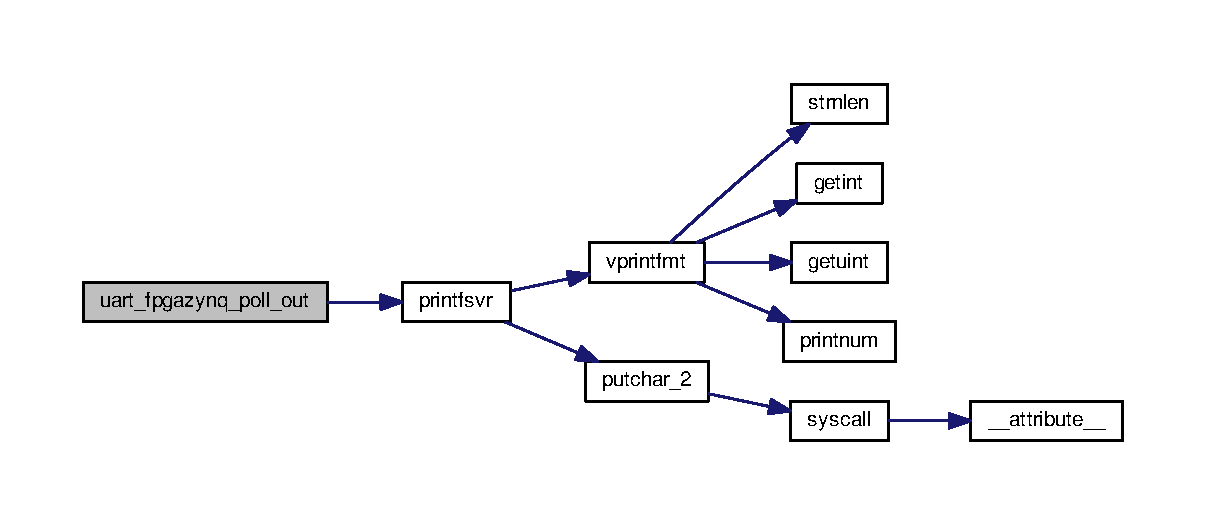
\includegraphics[width=350pt]{uart__fpgazynq_8c_a851bc4f05ccf668befa650b3ac66b67a_cgraph}
\end{center}
\end{figure}




\subsection{Variable Documentation}
\index{uart\+\_\+fpgazynq.\+c@{uart\+\_\+fpgazynq.\+c}!uart\+\_\+fpgazynq\+\_\+data\+\_\+0@{uart\+\_\+fpgazynq\+\_\+data\+\_\+0}}
\index{uart\+\_\+fpgazynq\+\_\+data\+\_\+0@{uart\+\_\+fpgazynq\+\_\+data\+\_\+0}!uart\+\_\+fpgazynq.\+c@{uart\+\_\+fpgazynq.\+c}}
\subsubsection[{\texorpdfstring{uart\+\_\+fpgazynq\+\_\+data\+\_\+0}{uart_fpgazynq_data_0}}]{\setlength{\rightskip}{0pt plus 5cm}struct {\bf uart\+\_\+fpgazynq\+\_\+data} uart\+\_\+fpgazynq\+\_\+data\+\_\+0\hspace{0.3cm}{\ttfamily [static]}}\hypertarget{uart__fpgazynq_8c_ab03ab7c5621c68576e871a67c76ccd9e}{}\label{uart__fpgazynq_8c_ab03ab7c5621c68576e871a67c76ccd9e}
{\bfseries Initial value\+:}
\begin{DoxyCode}
= \{
    .dummy = 0
\}
\end{DoxyCode}
\index{uart\+\_\+fpgazynq.\+c@{uart\+\_\+fpgazynq.\+c}!uart\+\_\+fpgazynq\+\_\+dev\+\_\+cfg\+\_\+0@{uart\+\_\+fpgazynq\+\_\+dev\+\_\+cfg\+\_\+0}}
\index{uart\+\_\+fpgazynq\+\_\+dev\+\_\+cfg\+\_\+0@{uart\+\_\+fpgazynq\+\_\+dev\+\_\+cfg\+\_\+0}!uart\+\_\+fpgazynq.\+c@{uart\+\_\+fpgazynq.\+c}}
\subsubsection[{\texorpdfstring{uart\+\_\+fpgazynq\+\_\+dev\+\_\+cfg\+\_\+0}{uart_fpgazynq_dev_cfg_0}}]{\setlength{\rightskip}{0pt plus 5cm}const struct {\bf uart\+\_\+fpgazynq\+\_\+device\+\_\+config} uart\+\_\+fpgazynq\+\_\+dev\+\_\+cfg\+\_\+0\hspace{0.3cm}{\ttfamily [static]}}\hypertarget{uart__fpgazynq_8c_a419c111714cb72b2b43363326490e957}{}\label{uart__fpgazynq_8c_a419c111714cb72b2b43363326490e957}
{\bfseries Initial value\+:}
\begin{DoxyCode}
= \{
    .dummy = 0
\}
\end{DoxyCode}
\index{uart\+\_\+fpgazynq.\+c@{uart\+\_\+fpgazynq.\+c}!uart\+\_\+fpgazynq\+\_\+driver\+\_\+api@{uart\+\_\+fpgazynq\+\_\+driver\+\_\+api}}
\index{uart\+\_\+fpgazynq\+\_\+driver\+\_\+api@{uart\+\_\+fpgazynq\+\_\+driver\+\_\+api}!uart\+\_\+fpgazynq.\+c@{uart\+\_\+fpgazynq.\+c}}
\subsubsection[{\texorpdfstring{uart\+\_\+fpgazynq\+\_\+driver\+\_\+api}{uart_fpgazynq_driver_api}}]{\setlength{\rightskip}{0pt plus 5cm}const struct uart\+\_\+driver\+\_\+api uart\+\_\+fpgazynq\+\_\+driver\+\_\+api\hspace{0.3cm}{\ttfamily [static]}}\hypertarget{uart__fpgazynq_8c_a98a5e63a49f40e30ecc0ec84d4df4364}{}\label{uart__fpgazynq_8c_a98a5e63a49f40e30ecc0ec84d4df4364}
{\bfseries Initial value\+:}
\begin{DoxyCode}
= \{
    .poll\_in          = \hyperlink{uart__fpgazynq_8c_a01a1487127b6b8ee6820644317e20a99}{uart\_fpgazynq\_poll\_in},   
    .poll\_out         = \hyperlink{uart__fpgazynq_8c_a851bc4f05ccf668befa650b3ac66b67a}{uart\_fpgazynq\_poll\_out},
    .err\_check        = NULL,
\}
\end{DoxyCode}

\hypertarget{irqtestperipheral_8c}{}\section{/home/timo/\+Software/zephyr-\/riscv\+\_\+dev/apps/irqperipheral\+\_\+test/src/drivers/irqtestperipheral/src/irqtestperipheral.c File Reference}
\label{irqtestperipheral_8c}\index{/home/timo/\+Software/zephyr-\/riscv\+\_\+dev/apps/irqperipheral\+\_\+test/src/drivers/irqtestperipheral/src/irqtestperipheral.\+c@{/home/timo/\+Software/zephyr-\/riscv\+\_\+dev/apps/irqperipheral\+\_\+test/src/drivers/irqtestperipheral/src/irqtestperipheral.\+c}}
{\ttfamily \#include \char`\"{}irqtestperipheral.\+h\char`\"{}}\\*
{\ttfamily \#include $<$soc.\+h$>$}\\*
{\ttfamily \#include $<$atomic.\+h$>$}\\*
{\ttfamily \#include $<$misc/printk.\+h$>$}\\*
{\ttfamily \#include $<$logging/sys\+\_\+log.\+h$>$}\\*
{\ttfamily \#include \char`\"{}cycles.\+h\char`\"{}}\\*
Include dependency graph for irqtestperipheral.\+c\+:\nopagebreak
\begin{figure}[H]
\begin{center}
\leavevmode
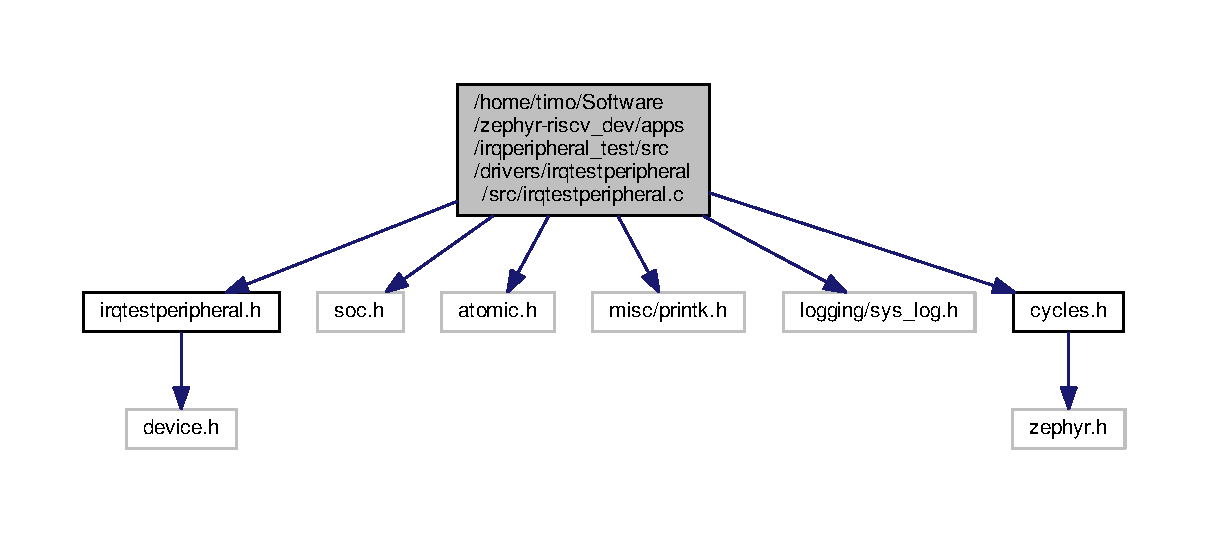
\includegraphics[width=350pt]{irqtestperipheral_8c__incl}
\end{center}
\end{figure}
\subsection*{Macros}
\begin{DoxyCompactItemize}
\item 
\#define \hyperlink{irqtestperipheral_8c_ac5b2cb2d6ae6b5526953a00f765a23e4}{S\+Y\+S\+\_\+\+L\+O\+G\+\_\+\+D\+O\+M\+A\+IN}~\char`\"{}Irq\+Test\+Peripheral\char`\"{}
\item 
\#define \hyperlink{irqtestperipheral_8c_a7e98264d6527b989d179c54a96034c88}{S\+Y\+S\+\_\+\+L\+O\+G\+\_\+\+L\+E\+V\+EL}~S\+Y\+S\+\_\+\+L\+O\+G\+\_\+\+L\+E\+V\+E\+L\+\_\+\+D\+E\+B\+UG
\item 
\#define \hyperlink{irqtestperipheral_8c_a618b1de4e1abb0efbf19ba5540d0aacc}{I\+R\+Q\+T\+\_\+\+I\+R\+Q\+\_\+0\+\_\+\+P\+IN}~-\/1
\item 
\#define \hyperlink{irqtestperipheral_8c_ae7640b78e59842b45e5b9707d6d05cd9}{I\+R\+Q\+T\+\_\+0\+\_\+\+I\+R\+Q\+\_\+0}~(R\+I\+S\+C\+V\+\_\+\+M\+A\+X\+\_\+\+G\+E\+N\+E\+R\+I\+C\+\_\+\+I\+RQ + \hyperlink{irqtestperipheral_8c_a618b1de4e1abb0efbf19ba5540d0aacc}{I\+R\+Q\+T\+\_\+\+I\+R\+Q\+\_\+0\+\_\+\+P\+IN})
\item 
\#define \hyperlink{irqtestperipheral_8c_a2c8e712612ca973426dc8fe11391be05}{I\+R\+Q\+T\+\_\+0\+\_\+\+I\+R\+Q\+\_\+1}~(R\+I\+S\+C\+V\+\_\+\+M\+A\+X\+\_\+\+G\+E\+N\+E\+R\+I\+C\+\_\+\+I\+RQ + \hyperlink{irqtestperipheral_8c_a618b1de4e1abb0efbf19ba5540d0aacc}{I\+R\+Q\+T\+\_\+\+I\+R\+Q\+\_\+0\+\_\+\+P\+IN} + 1)
\item 
\#define \hyperlink{irqtestperipheral_8c_a09b6f19186ade569c46edbde504cbde6}{I\+R\+Q\+T\+\_\+0\+\_\+\+I\+R\+Q\+\_\+2}~(R\+I\+S\+C\+V\+\_\+\+M\+A\+X\+\_\+\+G\+E\+N\+E\+R\+I\+C\+\_\+\+I\+RQ + \hyperlink{irqtestperipheral_8c_a618b1de4e1abb0efbf19ba5540d0aacc}{I\+R\+Q\+T\+\_\+\+I\+R\+Q\+\_\+0\+\_\+\+P\+IN} + 2)
\item 
\#define \hyperlink{irqtestperipheral_8c_aed4e1df2d3b72d111dbc36ebe9f1a051}{F\+E310\+\_\+\+I\+R\+Q\+T\+E\+S\+T\+E\+R\+\_\+0\+\_\+\+D\+S\+P\+\_\+0\+\_\+\+B\+A\+S\+E\+\_\+\+A\+D\+DR}~0x2000
\item 
\#define \hyperlink{irqtestperipheral_8c_a0046372ce9a45a3e7584dca75eccf0b0}{F\+E310\+\_\+\+I\+R\+Q\+T\+E\+S\+T\+E\+R\+\_\+0\+\_\+\+D\+S\+P\+\_\+1\+\_\+\+B\+A\+S\+E\+\_\+\+A\+D\+DR}~0x2010
\item 
\#define \hyperlink{irqtestperipheral_8c_aa4ad37e77a217e2fe72bbee0c6cd7a0f}{F\+E310\+\_\+\+I\+R\+Q\+T\+E\+S\+T\+E\+R\+\_\+0\+\_\+\+D\+S\+P\+\_\+2\+\_\+\+B\+A\+S\+E\+\_\+\+A\+D\+DR}~0x2020
\item 
\#define \hyperlink{irqtestperipheral_8c_a7330739b08f329f98d123eb0b39fcffd}{F\+E310\+\_\+\+I\+R\+Q\+T\+E\+S\+T\+E\+R\+\_\+0\+\_\+\+D\+S\+P\+\_\+3\+\_\+\+B\+A\+S\+E\+\_\+\+A\+D\+DR}~0x2030
\item 
\#define \hyperlink{irqtestperipheral_8c_aac3f21e92bb84a33fb3512aa09c96a8f}{F\+E310\+\_\+\+I\+R\+Q\+T\+E\+S\+T\+E\+R\+\_\+0\+\_\+\+D\+S\+P\+\_\+0\+\_\+\+S\+T\+A\+T\+U\+S\+\_\+\+B\+L\+O\+C\+K\+ED}~2
\item 
\#define \hyperlink{irqtestperipheral_8c_a533d9fd4806fede95f0776295c8b7bfc}{C\+O\+N\+F\+I\+G\+\_\+\+I\+R\+Q\+T\+E\+S\+T\+E\+R\+\_\+\+F\+E310\+\_\+0\+\_\+\+P\+R\+I\+O\+R\+I\+TY}~F\+E310\+\_\+\+P\+L\+I\+C\+\_\+\+M\+A\+X\+\_\+\+P\+R\+I\+O\+R\+I\+TY
\item 
\#define \hyperlink{irqtestperipheral_8c_ab5c3864067257693d9bef98c3fe8fc2b}{D\+E\+V\+\_\+\+C\+FG}(dev)~((const struct irqtester\+\_\+fe310\+\_\+config $\ast$ const)(dev)-\/$>$config-\/$>$config\+\_\+info)
\item 
\#define \hyperlink{irqtestperipheral_8c_ad5e999d5c89dc4c9a66ac43626f9c5d5}{D\+E\+V\+\_\+\+R\+E\+G\+S\+\_\+0}(dev)~((volatile struct irqtester\+\_\+fe310\+\_\+0\+\_\+t $\ast$)(\hyperlink{irqtestperipheral_8c_ab5c3864067257693d9bef98c3fe8fc2b}{D\+E\+V\+\_\+\+C\+FG}(dev))-\/$>$irqtester\+\_\+base\+\_\+addr\mbox{[}0\mbox{]})
\item 
\#define \hyperlink{irqtestperipheral_8c_a26f3776ec680c056ccb1377773d84acf}{D\+E\+V\+\_\+\+R\+E\+G\+S\+\_\+1}(dev)~((volatile struct irqtester\+\_\+fe310\+\_\+1\+\_\+t $\ast$)(\hyperlink{irqtestperipheral_8c_ab5c3864067257693d9bef98c3fe8fc2b}{D\+E\+V\+\_\+\+C\+FG}(dev))-\/$>$irqtester\+\_\+base\+\_\+addr\mbox{[}1\mbox{]})
\item 
\#define \hyperlink{irqtestperipheral_8c_a745df4fe3648b54e304b8588aba922e8}{D\+E\+V\+\_\+\+R\+E\+G\+S\+\_\+2}(dev)~((volatile struct irqtester\+\_\+fe310\+\_\+2\+\_\+t $\ast$)(\hyperlink{irqtestperipheral_8c_ab5c3864067257693d9bef98c3fe8fc2b}{D\+E\+V\+\_\+\+C\+FG}(dev))-\/$>$irqtester\+\_\+base\+\_\+addr\mbox{[}2\mbox{]})
\item 
\#define \hyperlink{irqtestperipheral_8c_af181f6a8bfa50e654f744031f5111a6c}{D\+E\+V\+\_\+\+R\+E\+G\+S\+\_\+3}(dev)~((volatile struct irqtester\+\_\+fe310\+\_\+3\+\_\+t $\ast$)(\hyperlink{irqtestperipheral_8c_ab5c3864067257693d9bef98c3fe8fc2b}{D\+E\+V\+\_\+\+C\+FG}(dev))-\/$>$irqtester\+\_\+base\+\_\+addr\mbox{[}3\mbox{]})
\item 
\#define \hyperlink{irqtestperipheral_8c_aa90b045b0cf3a7fe70c69ba16eb135cc}{D\+E\+V\+\_\+\+D\+A\+TA}(dev)~((struct irqtester\+\_\+fe310\+\_\+data $\ast$)(dev)-\/$>$driver\+\_\+data)
\item 
\#define \hyperlink{irqtestperipheral_8c_a01901b6f13f37b6c03cd37a0e75eadd4}{D\+EV}()~irqtester\+\_\+fe310\+\_\+data0.\+\_\+drv\+\_\+handle
\item 
\#define \hyperlink{irqtestperipheral_8c_ac85ffac15e6947e9fb5acf752fba7207}{L\+E\+N\+\_\+\+A\+R\+R\+AY}(x)~((sizeof(x)/sizeof(0\mbox{[}x\mbox{]})) / ((size\+\_\+t)(!(sizeof(x) \% sizeof(0\mbox{[}x\mbox{]})))))
\item 
\#define \hyperlink{irqtestperipheral_8c_a3172e049ce29531f493508355528ffab}{N\+U\+M\+\_\+\+V\+A\+LS}()~(\hyperlink{state__manager_8c_ac85ffac15e6947e9fb5acf752fba7207}{L\+E\+N\+\_\+\+A\+R\+R\+AY}(\hyperlink{irqtestperipheral_8c_a425ae3473e646745e0d280c10af20d7f}{\+\_\+values\+\_\+uint}) + \hyperlink{state__manager_8c_ac85ffac15e6947e9fb5acf752fba7207}{L\+E\+N\+\_\+\+A\+R\+R\+AY}(\hyperlink{irqtestperipheral_8c_a23fe4b9972f3fd20c5606617960f5230}{\+\_\+values\+\_\+int}) +  \hyperlink{state__manager_8c_ac85ffac15e6947e9fb5acf752fba7207}{L\+E\+N\+\_\+\+A\+R\+R\+AY}(\hyperlink{irqtestperipheral_8c_a7b19da922c8e92d1fc4e69ba9050c7e6}{\+\_\+values\+\_\+bool}))
\item 
\#define \hyperlink{irqtestperipheral_8c_a4dd6c593e20015ba9025dbe37f8f94a2}{I\+R\+Q1\+\_\+\+C\+L\+E\+AR}~0x201C
\item 
\#define \hyperlink{irqtestperipheral_8c_ac4578ab4bc743e3ec3bcbec63cfd60df}{I\+R\+Q2\+\_\+\+C\+L\+E\+AR}~0x202C
\end{DoxyCompactItemize}
\subsection*{Enumerations}
\begin{DoxyCompactItemize}
\item 
enum \hyperlink{irqtestperipheral_8c_ab6b306ef981f5e21bb41ea2c2dbe8cd9}{flags} \{ \\*
\hyperlink{irqtestperipheral_8c_ab6b306ef981f5e21bb41ea2c2dbe8cd9a0a09fd9d2fea0ac766896b4cb3e96803}{I\+R\+Q\+T\+\_\+\+Q\+U\+E\+U\+E\+\_\+\+R\+X\+\_\+\+E\+N\+A\+B\+L\+ED}, 
\hyperlink{irqtestperipheral_8c_ab6b306ef981f5e21bb41ea2c2dbe8cd9a233cfd37e793f2693b9c42cd7cb3cd0a}{I\+R\+Q\+T\+\_\+\+F\+I\+F\+O\+\_\+\+R\+X\+\_\+\+E\+N\+A\+B\+L\+ED}, 
\hyperlink{irqtestperipheral_8c_ab6b306ef981f5e21bb41ea2c2dbe8cd9aba03d680731db9d7d4c71411e5b9d417}{I\+R\+Q\+T\+\_\+\+S\+E\+M\+A\+R\+R\+\_\+\+R\+X\+\_\+\+E\+N\+A\+B\+L\+ED}, 
\hyperlink{irqtestperipheral_8c_ab6b306ef981f5e21bb41ea2c2dbe8cd9aa1208dd5c4755e40f3d93161f3eaf52e}{I\+R\+Q\+T\+\_\+\+V\+A\+L\+F\+L\+A\+G\+S\+\_\+\+R\+X\+\_\+\+E\+N\+A\+B\+L\+ED}, 
\\*
\hyperlink{irqtestperipheral_8c_ab6b306ef981f5e21bb41ea2c2dbe8cd9a48a03cb0b3da425f8d3a80891524cf83}{\+\_\+\+I\+R\+Q\+T\+\_\+\+N\+U\+M\+\_\+\+F\+L\+A\+GS}
 \}
\end{DoxyCompactItemize}
\subsection*{Functions}
\begin{DoxyCompactItemize}
\item 
static \hyperlink{irqtestperipheral_8h_a6354e3cbd47a9004937a59f50ede5080}{irqt\+\_\+val\+\_\+type\+\_\+t} \hyperlink{irqtestperipheral_8c_a15420b03ab67124ddc6d1b4f63f32309}{id\+\_\+2\+\_\+type} (\hyperlink{irqtestperipheral_8h_a3485d29696b63704b7a6454519c3d0c5}{irqt\+\_\+val\+\_\+id\+\_\+t} id)
\item 
static \hyperlink{irqtestperipheral_8h_a6354e3cbd47a9004937a59f50ede5080}{irqt\+\_\+val\+\_\+type\+\_\+t} \hyperlink{irqtestperipheral_8c_aacd45cbca76d5cb252b111e2e064a3e0}{id\+\_\+2\+\_\+type\+\_\+fast} (\hyperlink{irqtestperipheral_8h_a3485d29696b63704b7a6454519c3d0c5}{irqt\+\_\+val\+\_\+id\+\_\+t} id)
\item 
static int \hyperlink{irqtestperipheral_8c_a3205d750d033a40f72392b0d638b9070}{id\+\_\+2\+\_\+index} (\hyperlink{irqtestperipheral_8h_a3485d29696b63704b7a6454519c3d0c5}{irqt\+\_\+val\+\_\+id\+\_\+t} id)
\item 
static int \hyperlink{irqtestperipheral_8c_aae36b616bf3ffc8134b83f3e168bdf0e}{id\+\_\+2\+\_\+index\+\_\+fast} (\hyperlink{irqtestperipheral_8h_a3485d29696b63704b7a6454519c3d0c5}{irqt\+\_\+val\+\_\+id\+\_\+t} id, \hyperlink{irqtestperipheral_8h_a6354e3cbd47a9004937a59f50ede5080}{irqt\+\_\+val\+\_\+type\+\_\+t} type)
\item 
static \hyperlink{irqtestperipheral_8h_a53f93f474fe7c9fa2072c6e9cea3d6ef}{irqt\+\_\+irq\+\_\+id\+\_\+t} \hyperlink{irqtestperipheral_8c_abda9b87261994cc7417d4db872faa8f2}{\+\_\+get\+\_\+irq\+\_\+id} ()
\item 
static bool \hyperlink{irqtestperipheral_8c_a4f458d7df910b1501b2afc15c685dfe2}{test\+\_\+flag} (struct device $\ast$dev, int drv\+\_\+flag)
\item 
static bool \hyperlink{irqtestperipheral_8c_a023df633a0cf154035fced51999c3f66}{test\+\_\+any\+\_\+send\+\_\+flag} (struct device $\ast$dev)
\begin{DoxyCompactList}\small\item\em Test whether any flags for event sending are set. This excludes valflags, as they don\textquotesingle{}t issue events. \end{DoxyCompactList}\item 
static void \hyperlink{irqtestperipheral_8c_ab157fe508c290d5e05fc878db1c936f0}{irqtester\+\_\+fe310\+\_\+irq\+\_\+handler} (void $\ast$arg)
\item 
static void \hyperlink{irqtestperipheral_8c_aea8fe973b67fd1364c333f4ba595b6db}{send\+\_\+event\+\_\+rx} (struct device $\ast$dev, struct \hyperlink{struct_drv_event}{Drv\+Event} $\ast$evt)
\item 
static void \hyperlink{irqtestperipheral_8c_a95991437cd831bd6ad077bc6382059ee}{flag\+\_\+event\+\_\+rx} (struct device $\ast$dev, struct \hyperlink{struct_drv_event}{Drv\+Event} $\ast$evt)
\begin{DoxyCompactList}\small\item\em Sets the (atomic) flag to indicate to higher level applications that event occured. \end{DoxyCompactList}\item 
static void \hyperlink{irqtestperipheral_8c_a8b6a6dc9fd115e8c6346549531d43199}{\+\_\+irq\+\_\+gen\+\_\+handler} (void)
\begin{DoxyCompactList}\small\item\em Default I\+SR set up in driver init. Serves all I\+R\+Qs of irqtester. \end{DoxyCompactList}\item 
int \hyperlink{irqtestperipheral_8c_a1d2af0fa1a30580646c700e462bf063f}{irqtester\+\_\+fe310\+\_\+reset\+\_\+hw} (struct device $\ast$dev)
\begin{DoxyCompactList}\small\item\em Reset all hw regs but \textquotesingle{}enable\textquotesingle{} to 0. Doesn\textquotesingle{}t reset internal and output regs! \end{DoxyCompactList}\item 
int \hyperlink{irqtestperipheral_8c_a46f10c3e9b63404c15f52ab375a28977}{irqtester\+\_\+fe310\+\_\+get\+\_\+val} (\hyperlink{irqtestperipheral_8h_a3485d29696b63704b7a6454519c3d0c5}{irqt\+\_\+val\+\_\+id\+\_\+t} id, void $\ast$res\+\_\+value)
\begin{DoxyCompactList}\small\item\em Thread safe generic (by id) getter for values of generic type from driver memory pools. \end{DoxyCompactList}\item 
int \hyperlink{irqtestperipheral_8c_a4e987f34af28aea872408b2412339ad7}{irqtester\+\_\+fe310\+\_\+get\+\_\+val\+\_\+uint} (\hyperlink{irqtestperipheral_8h_a3485d29696b63704b7a6454519c3d0c5}{irqt\+\_\+val\+\_\+id\+\_\+t} id, void $\ast$res\+\_\+value)
\begin{DoxyCompactList}\small\item\em Thread safe generic (by id) getter for values of uint type from driver memory pools. \end{DoxyCompactList}\item 
u32\+\_\+t \hyperlink{irqtestperipheral_8c_a2033394f5344ffe1c16f65be91851217}{irqtester\+\_\+fe310\+\_\+get\+\_\+val\+\_\+uint\+\_\+raw} (\hyperlink{irqtestperipheral_8h_a3485d29696b63704b7a6454519c3d0c5}{irqt\+\_\+val\+\_\+id\+\_\+t} id)
\begin{DoxyCompactList}\small\item\em Thread safe generic (by id) getter for values of uint type from driver memory pools. For perforamnce reasons, use return value instread a passed container for result. \end{DoxyCompactList}\item 
int \hyperlink{irqtestperipheral_8c_a1356feef1a2dbd5af9d5f6c19e2d86a6}{irqtester\+\_\+fe310\+\_\+set\+\_\+reg\+\_\+fast} (struct device $\ast$dev, \hyperlink{irqtestperipheral_8h_a3485d29696b63704b7a6454519c3d0c5}{irqt\+\_\+val\+\_\+id\+\_\+t} id, void $\ast$set\+\_\+val)
\begin{DoxyCompactList}\small\item\em Non-\/\+Thread safe, generic setter for device registers. Only works for regs which have a driver mem pool entry. \end{DoxyCompactList}\item 
int \hyperlink{irqtestperipheral_8c_ace3058eeacfe748758334352a992716e}{irqtester\+\_\+fe310\+\_\+set\+\_\+reg\+\_\+uint\+\_\+fast} (struct device $\ast$dev, \hyperlink{irqtestperipheral_8h_a3485d29696b63704b7a6454519c3d0c5}{irqt\+\_\+val\+\_\+id\+\_\+t} id, void $\ast$set\+\_\+val)
\begin{DoxyCompactList}\small\item\em Thread un-\/safe generic (by id) setter for hw regs of uint type. \end{DoxyCompactList}\item 
int \hyperlink{irqtestperipheral_8c_a508afd9a858251ac9dbd15fba94e4301}{irqtester\+\_\+fe310\+\_\+set\+\_\+reg} (struct device $\ast$dev, \hyperlink{irqtestperipheral_8h_a3485d29696b63704b7a6454519c3d0c5}{irqt\+\_\+val\+\_\+id\+\_\+t} id, void $\ast$set\+\_\+val)
\begin{DoxyCompactList}\small\item\em Thread safe, generic setter for device registers. Only works for regs which have a driver mem pool entry. \end{DoxyCompactList}\item 
int \hyperlink{irqtestperipheral_8c_a987670a27b50999e651f384e6b04e582}{irqtester\+\_\+fe310\+\_\+get\+\_\+reg} (struct device $\ast$dev, \hyperlink{irqtestperipheral_8h_a3485d29696b63704b7a6454519c3d0c5}{irqt\+\_\+val\+\_\+id\+\_\+t} id, void $\ast$res\+\_\+val)
\begin{DoxyCompactList}\small\item\em Non-\/thread safe, generic getter for device (output) registers. Only works for regs which are loaded to driver mem pools. \end{DoxyCompactList}\item 
bool \hyperlink{irqtestperipheral_8c_ae593bcc753fee4064e23b3e290e5f27d}{irqtester\+\_\+fe310\+\_\+test\+\_\+valflag} (struct device $\ast$dev, \hyperlink{irqtestperipheral_8h_a3485d29696b63704b7a6454519c3d0c5}{irqt\+\_\+val\+\_\+id\+\_\+t} id)
\begin{DoxyCompactList}\small\item\em Test whether a value was flagged ready to get\+\_\+val() from driver memory. \end{DoxyCompactList}\item 
void \hyperlink{irqtestperipheral_8c_a997c5939bc6f47d246540c69ff49733d}{irqtester\+\_\+fe310\+\_\+clear\+\_\+all\+\_\+valflags} (struct device $\ast$dev)
\begin{DoxyCompactList}\small\item\em Clear all flags. \end{DoxyCompactList}\item 
int \hyperlink{irqtestperipheral_8c_a8b03f7c9aff5996a16845f0e2d1e6937}{irqtester\+\_\+fe310\+\_\+register\+\_\+queue\+\_\+rx} (struct device $\ast$dev, struct k\+\_\+msgq $\ast$queue)
\begin{DoxyCompactList}\small\item\em Provide a handle to a queue to receive msgs from the driver there. \end{DoxyCompactList}\item 
int \hyperlink{irqtestperipheral_8c_ace3a40543bbebb04e1324fbfa9f60275}{irqtester\+\_\+fe310\+\_\+register\+\_\+fifo\+\_\+rx} (struct device $\ast$dev, struct k\+\_\+fifo $\ast$queue)
\begin{DoxyCompactList}\small\item\em Provide a handle to a fifo to receive msgs from the driver there. \end{DoxyCompactList}\item 
int \hyperlink{irqtestperipheral_8c_ae82ab1a2ea6ec7bd8f6b43530d1419a5}{irqtester\+\_\+fe310\+\_\+register\+\_\+sem\+\_\+arr\+\_\+rx} (struct device $\ast$dev, struct k\+\_\+sem $\ast$sem, struct \hyperlink{struct_drv_event}{Drv\+Event} evt\+\_\+arr\mbox{[}$\,$\mbox{]}, int len)
\begin{DoxyCompactList}\small\item\em Provide a handle to a semaphore and an even array to receive msgs from the driver there. \end{DoxyCompactList}\item 
int \hyperlink{irqtestperipheral_8c_a9c8c75c9c4603bdccd5bdcf3038d3c49}{irqtester\+\_\+fe310\+\_\+enable\+\_\+queue\+\_\+rx} (struct device $\ast$dev)
\begin{DoxyCompactList}\small\item\em Enable previously registered queue\+\_\+rx for sending driver events to. \end{DoxyCompactList}\item 
int \hyperlink{irqtestperipheral_8c_aff89ef81c09b5a1c7631fc236b671e7d}{irqtester\+\_\+fe310\+\_\+enable\+\_\+fifo\+\_\+rx} (struct device $\ast$dev)
\begin{DoxyCompactList}\small\item\em Enable previously registered fifo\+\_\+rx for sending driver events to. \end{DoxyCompactList}\item 
int \hyperlink{irqtestperipheral_8c_acc15d23902deee0d82e20e237a526275}{irqtester\+\_\+fe310\+\_\+enable\+\_\+sem\+\_\+arr\+\_\+rx} (struct device $\ast$dev)
\begin{DoxyCompactList}\small\item\em Enable previously registered semaphore plus event array for sending driver events to. \end{DoxyCompactList}\item 
int \hyperlink{irqtestperipheral_8c_ace5f0827eb25f735e652ab09f4cbe3b2}{irqtester\+\_\+fe310\+\_\+enable\+\_\+valflags\+\_\+rx} (struct device $\ast$dev)
\begin{DoxyCompactList}\small\item\em Enables flags for indicating load of harware values to driver memory. \end{DoxyCompactList}\item 
int \hyperlink{irqtestperipheral_8c_a254eae890ba510e5e473a046407ba618}{irqtester\+\_\+fe310\+\_\+receive\+\_\+evt\+\_\+from\+\_\+arr} (struct device $\ast$dev, struct \hyperlink{struct_drv_event}{Drv\+Event} $\ast$res, s32\+\_\+t timeout)
\begin{DoxyCompactList}\small\item\em If using semaphore plus event array, call this to wait and receive an event. \end{DoxyCompactList}\item 
int \hyperlink{irqtestperipheral_8c_ab47c9b38275ed5cb45931e907725dc06}{irqtester\+\_\+fe310\+\_\+purge\+\_\+rx} (struct device $\ast$dev)
\begin{DoxyCompactList}\small\item\em Reset all objects related to receiving data from this driver. \end{DoxyCompactList}\item 
void \hyperlink{irqtestperipheral_8c_ae5817f51846271d1228fa02cc0e1726e}{irqtester\+\_\+fe310\+\_\+dbgprint\+\_\+event} (struct device $\ast$dev, struct \hyperlink{struct_drv_event}{Drv\+Event} $\ast$evt)
\begin{DoxyCompactList}\small\item\em Print information about an event as a debug log message. \end{DoxyCompactList}\item 
int \hyperlink{irqtestperipheral_8c_ac1e81dcf0faf4348a6121675f46553ff}{irqtester\+\_\+fe310\+\_\+fire} (struct device $\ast$dev)
\item 
void \hyperlink{irqtestperipheral_8c_a0bd81b8a8b0a9eb85658ffcfe6c0a7e5}{irqtester\+\_\+fe310\+\_\+fire\+\_\+1} (struct device $\ast$dev)
\begin{DoxyCompactList}\small\item\em Need to set regs num\+\_\+rep\+\_\+1 and period\+\_\+1 first. \end{DoxyCompactList}\item 
int \hyperlink{irqtestperipheral_8c_a3f0daddddbc00ed4d3195cd85ba1acae}{irqtester\+\_\+fe310\+\_\+fire\+\_\+2} (struct device $\ast$dev)
\begin{DoxyCompactList}\small\item\em Need to set regs num\+\_\+rep\+\_\+2 and period\+\_\+2 first. \end{DoxyCompactList}\item 
void \hyperlink{irqtestperipheral_8c_a260bbaa36d21fbbf0441d4d15fe1a5e0}{irqtester\+\_\+fe310\+\_\+clear\+\_\+1} (struct device $\ast$dev)
\item 
void \hyperlink{irqtestperipheral_8c_ac28383949304b588aecac37c6d6ea538}{irqtester\+\_\+fe310\+\_\+clear\+\_\+2} (struct device $\ast$dev)
\end{DoxyCompactItemize}
\subsection*{Variables}
\begin{DoxyCompactItemize}
\item 
static struct \hyperlink{struct_drv_value__uint}{Drv\+Value\+\_\+uint} \hyperlink{irqtestperipheral_8c_a425ae3473e646745e0d280c10af20d7f}{\+\_\+values\+\_\+uint} \mbox{[}$\,$\mbox{]}
\item 
static struct \hyperlink{struct_drv_value__int}{Drv\+Value\+\_\+int} \hyperlink{irqtestperipheral_8c_a23fe4b9972f3fd20c5606617960f5230}{\+\_\+values\+\_\+int} \mbox{[}$\,$\mbox{]}
\item 
static struct \hyperlink{struct_drv_value__bool}{Drv\+Value\+\_\+bool} \hyperlink{irqtestperipheral_8c_a7b19da922c8e92d1fc4e69ba9050c7e6}{\+\_\+values\+\_\+bool} \mbox{[}$\,$\mbox{]}
\end{DoxyCompactItemize}


\subsection{Detailed Description}
Driver for Irq\+Test\+Peripheral hw revision 3. Singleton, only register one instance with kernel! 

\subsection{Macro Definition Documentation}
\index{irqtestperipheral.\+c@{irqtestperipheral.\+c}!C\+O\+N\+F\+I\+G\+\_\+\+I\+R\+Q\+T\+E\+S\+T\+E\+R\+\_\+\+F\+E310\+\_\+0\+\_\+\+P\+R\+I\+O\+R\+I\+TY@{C\+O\+N\+F\+I\+G\+\_\+\+I\+R\+Q\+T\+E\+S\+T\+E\+R\+\_\+\+F\+E310\+\_\+0\+\_\+\+P\+R\+I\+O\+R\+I\+TY}}
\index{C\+O\+N\+F\+I\+G\+\_\+\+I\+R\+Q\+T\+E\+S\+T\+E\+R\+\_\+\+F\+E310\+\_\+0\+\_\+\+P\+R\+I\+O\+R\+I\+TY@{C\+O\+N\+F\+I\+G\+\_\+\+I\+R\+Q\+T\+E\+S\+T\+E\+R\+\_\+\+F\+E310\+\_\+0\+\_\+\+P\+R\+I\+O\+R\+I\+TY}!irqtestperipheral.\+c@{irqtestperipheral.\+c}}
\subsubsection[{\texorpdfstring{C\+O\+N\+F\+I\+G\+\_\+\+I\+R\+Q\+T\+E\+S\+T\+E\+R\+\_\+\+F\+E310\+\_\+0\+\_\+\+P\+R\+I\+O\+R\+I\+TY}{CONFIG_IRQTESTER_FE310_0_PRIORITY}}]{\setlength{\rightskip}{0pt plus 5cm}\#define C\+O\+N\+F\+I\+G\+\_\+\+I\+R\+Q\+T\+E\+S\+T\+E\+R\+\_\+\+F\+E310\+\_\+0\+\_\+\+P\+R\+I\+O\+R\+I\+TY~F\+E310\+\_\+\+P\+L\+I\+C\+\_\+\+M\+A\+X\+\_\+\+P\+R\+I\+O\+R\+I\+TY}\hypertarget{irqtestperipheral_8c_a533d9fd4806fede95f0776295c8b7bfc}{}\label{irqtestperipheral_8c_a533d9fd4806fede95f0776295c8b7bfc}
\index{irqtestperipheral.\+c@{irqtestperipheral.\+c}!D\+EV@{D\+EV}}
\index{D\+EV@{D\+EV}!irqtestperipheral.\+c@{irqtestperipheral.\+c}}
\subsubsection[{\texorpdfstring{D\+EV}{DEV}}]{\setlength{\rightskip}{0pt plus 5cm}\#define D\+EV(
\begin{DoxyParamCaption}
{}
\end{DoxyParamCaption}
)~irqtester\+\_\+fe310\+\_\+data0.\+\_\+drv\+\_\+handle}\hypertarget{irqtestperipheral_8c_a01901b6f13f37b6c03cd37a0e75eadd4}{}\label{irqtestperipheral_8c_a01901b6f13f37b6c03cd37a0e75eadd4}
\index{irqtestperipheral.\+c@{irqtestperipheral.\+c}!D\+E\+V\+\_\+\+C\+FG@{D\+E\+V\+\_\+\+C\+FG}}
\index{D\+E\+V\+\_\+\+C\+FG@{D\+E\+V\+\_\+\+C\+FG}!irqtestperipheral.\+c@{irqtestperipheral.\+c}}
\subsubsection[{\texorpdfstring{D\+E\+V\+\_\+\+C\+FG}{DEV_CFG}}]{\setlength{\rightskip}{0pt plus 5cm}\#define D\+E\+V\+\_\+\+C\+FG(
\begin{DoxyParamCaption}
\item[{}]{dev}
\end{DoxyParamCaption}
)~((const struct irqtester\+\_\+fe310\+\_\+config $\ast$ const)(dev)-\/$>$config-\/$>$config\+\_\+info)}\hypertarget{irqtestperipheral_8c_ab5c3864067257693d9bef98c3fe8fc2b}{}\label{irqtestperipheral_8c_ab5c3864067257693d9bef98c3fe8fc2b}
\index{irqtestperipheral.\+c@{irqtestperipheral.\+c}!D\+E\+V\+\_\+\+D\+A\+TA@{D\+E\+V\+\_\+\+D\+A\+TA}}
\index{D\+E\+V\+\_\+\+D\+A\+TA@{D\+E\+V\+\_\+\+D\+A\+TA}!irqtestperipheral.\+c@{irqtestperipheral.\+c}}
\subsubsection[{\texorpdfstring{D\+E\+V\+\_\+\+D\+A\+TA}{DEV_DATA}}]{\setlength{\rightskip}{0pt plus 5cm}\#define D\+E\+V\+\_\+\+D\+A\+TA(
\begin{DoxyParamCaption}
\item[{}]{dev}
\end{DoxyParamCaption}
)~((struct irqtester\+\_\+fe310\+\_\+data $\ast$)(dev)-\/$>$driver\+\_\+data)}\hypertarget{irqtestperipheral_8c_aa90b045b0cf3a7fe70c69ba16eb135cc}{}\label{irqtestperipheral_8c_aa90b045b0cf3a7fe70c69ba16eb135cc}
\index{irqtestperipheral.\+c@{irqtestperipheral.\+c}!D\+E\+V\+\_\+\+R\+E\+G\+S\+\_\+0@{D\+E\+V\+\_\+\+R\+E\+G\+S\+\_\+0}}
\index{D\+E\+V\+\_\+\+R\+E\+G\+S\+\_\+0@{D\+E\+V\+\_\+\+R\+E\+G\+S\+\_\+0}!irqtestperipheral.\+c@{irqtestperipheral.\+c}}
\subsubsection[{\texorpdfstring{D\+E\+V\+\_\+\+R\+E\+G\+S\+\_\+0}{DEV_REGS_0}}]{\setlength{\rightskip}{0pt plus 5cm}\#define D\+E\+V\+\_\+\+R\+E\+G\+S\+\_\+0(
\begin{DoxyParamCaption}
\item[{}]{dev}
\end{DoxyParamCaption}
)~((volatile struct irqtester\+\_\+fe310\+\_\+0\+\_\+t $\ast$)({\bf D\+E\+V\+\_\+\+C\+FG}(dev))-\/$>$irqtester\+\_\+base\+\_\+addr\mbox{[}0\mbox{]})}\hypertarget{irqtestperipheral_8c_ad5e999d5c89dc4c9a66ac43626f9c5d5}{}\label{irqtestperipheral_8c_ad5e999d5c89dc4c9a66ac43626f9c5d5}
\index{irqtestperipheral.\+c@{irqtestperipheral.\+c}!D\+E\+V\+\_\+\+R\+E\+G\+S\+\_\+1@{D\+E\+V\+\_\+\+R\+E\+G\+S\+\_\+1}}
\index{D\+E\+V\+\_\+\+R\+E\+G\+S\+\_\+1@{D\+E\+V\+\_\+\+R\+E\+G\+S\+\_\+1}!irqtestperipheral.\+c@{irqtestperipheral.\+c}}
\subsubsection[{\texorpdfstring{D\+E\+V\+\_\+\+R\+E\+G\+S\+\_\+1}{DEV_REGS_1}}]{\setlength{\rightskip}{0pt plus 5cm}\#define D\+E\+V\+\_\+\+R\+E\+G\+S\+\_\+1(
\begin{DoxyParamCaption}
\item[{}]{dev}
\end{DoxyParamCaption}
)~((volatile struct irqtester\+\_\+fe310\+\_\+1\+\_\+t $\ast$)({\bf D\+E\+V\+\_\+\+C\+FG}(dev))-\/$>$irqtester\+\_\+base\+\_\+addr\mbox{[}1\mbox{]})}\hypertarget{irqtestperipheral_8c_a26f3776ec680c056ccb1377773d84acf}{}\label{irqtestperipheral_8c_a26f3776ec680c056ccb1377773d84acf}
\index{irqtestperipheral.\+c@{irqtestperipheral.\+c}!D\+E\+V\+\_\+\+R\+E\+G\+S\+\_\+2@{D\+E\+V\+\_\+\+R\+E\+G\+S\+\_\+2}}
\index{D\+E\+V\+\_\+\+R\+E\+G\+S\+\_\+2@{D\+E\+V\+\_\+\+R\+E\+G\+S\+\_\+2}!irqtestperipheral.\+c@{irqtestperipheral.\+c}}
\subsubsection[{\texorpdfstring{D\+E\+V\+\_\+\+R\+E\+G\+S\+\_\+2}{DEV_REGS_2}}]{\setlength{\rightskip}{0pt plus 5cm}\#define D\+E\+V\+\_\+\+R\+E\+G\+S\+\_\+2(
\begin{DoxyParamCaption}
\item[{}]{dev}
\end{DoxyParamCaption}
)~((volatile struct irqtester\+\_\+fe310\+\_\+2\+\_\+t $\ast$)({\bf D\+E\+V\+\_\+\+C\+FG}(dev))-\/$>$irqtester\+\_\+base\+\_\+addr\mbox{[}2\mbox{]})}\hypertarget{irqtestperipheral_8c_a745df4fe3648b54e304b8588aba922e8}{}\label{irqtestperipheral_8c_a745df4fe3648b54e304b8588aba922e8}
\index{irqtestperipheral.\+c@{irqtestperipheral.\+c}!D\+E\+V\+\_\+\+R\+E\+G\+S\+\_\+3@{D\+E\+V\+\_\+\+R\+E\+G\+S\+\_\+3}}
\index{D\+E\+V\+\_\+\+R\+E\+G\+S\+\_\+3@{D\+E\+V\+\_\+\+R\+E\+G\+S\+\_\+3}!irqtestperipheral.\+c@{irqtestperipheral.\+c}}
\subsubsection[{\texorpdfstring{D\+E\+V\+\_\+\+R\+E\+G\+S\+\_\+3}{DEV_REGS_3}}]{\setlength{\rightskip}{0pt plus 5cm}\#define D\+E\+V\+\_\+\+R\+E\+G\+S\+\_\+3(
\begin{DoxyParamCaption}
\item[{}]{dev}
\end{DoxyParamCaption}
)~((volatile struct irqtester\+\_\+fe310\+\_\+3\+\_\+t $\ast$)({\bf D\+E\+V\+\_\+\+C\+FG}(dev))-\/$>$irqtester\+\_\+base\+\_\+addr\mbox{[}3\mbox{]})}\hypertarget{irqtestperipheral_8c_af181f6a8bfa50e654f744031f5111a6c}{}\label{irqtestperipheral_8c_af181f6a8bfa50e654f744031f5111a6c}
\index{irqtestperipheral.\+c@{irqtestperipheral.\+c}!F\+E310\+\_\+\+I\+R\+Q\+T\+E\+S\+T\+E\+R\+\_\+0\+\_\+\+D\+S\+P\+\_\+0\+\_\+\+B\+A\+S\+E\+\_\+\+A\+D\+DR@{F\+E310\+\_\+\+I\+R\+Q\+T\+E\+S\+T\+E\+R\+\_\+0\+\_\+\+D\+S\+P\+\_\+0\+\_\+\+B\+A\+S\+E\+\_\+\+A\+D\+DR}}
\index{F\+E310\+\_\+\+I\+R\+Q\+T\+E\+S\+T\+E\+R\+\_\+0\+\_\+\+D\+S\+P\+\_\+0\+\_\+\+B\+A\+S\+E\+\_\+\+A\+D\+DR@{F\+E310\+\_\+\+I\+R\+Q\+T\+E\+S\+T\+E\+R\+\_\+0\+\_\+\+D\+S\+P\+\_\+0\+\_\+\+B\+A\+S\+E\+\_\+\+A\+D\+DR}!irqtestperipheral.\+c@{irqtestperipheral.\+c}}
\subsubsection[{\texorpdfstring{F\+E310\+\_\+\+I\+R\+Q\+T\+E\+S\+T\+E\+R\+\_\+0\+\_\+\+D\+S\+P\+\_\+0\+\_\+\+B\+A\+S\+E\+\_\+\+A\+D\+DR}{FE310_IRQTESTER_0_DSP_0_BASE_ADDR}}]{\setlength{\rightskip}{0pt plus 5cm}\#define F\+E310\+\_\+\+I\+R\+Q\+T\+E\+S\+T\+E\+R\+\_\+0\+\_\+\+D\+S\+P\+\_\+0\+\_\+\+B\+A\+S\+E\+\_\+\+A\+D\+DR~0x2000}\hypertarget{irqtestperipheral_8c_aed4e1df2d3b72d111dbc36ebe9f1a051}{}\label{irqtestperipheral_8c_aed4e1df2d3b72d111dbc36ebe9f1a051}
\index{irqtestperipheral.\+c@{irqtestperipheral.\+c}!F\+E310\+\_\+\+I\+R\+Q\+T\+E\+S\+T\+E\+R\+\_\+0\+\_\+\+D\+S\+P\+\_\+0\+\_\+\+S\+T\+A\+T\+U\+S\+\_\+\+B\+L\+O\+C\+K\+ED@{F\+E310\+\_\+\+I\+R\+Q\+T\+E\+S\+T\+E\+R\+\_\+0\+\_\+\+D\+S\+P\+\_\+0\+\_\+\+S\+T\+A\+T\+U\+S\+\_\+\+B\+L\+O\+C\+K\+ED}}
\index{F\+E310\+\_\+\+I\+R\+Q\+T\+E\+S\+T\+E\+R\+\_\+0\+\_\+\+D\+S\+P\+\_\+0\+\_\+\+S\+T\+A\+T\+U\+S\+\_\+\+B\+L\+O\+C\+K\+ED@{F\+E310\+\_\+\+I\+R\+Q\+T\+E\+S\+T\+E\+R\+\_\+0\+\_\+\+D\+S\+P\+\_\+0\+\_\+\+S\+T\+A\+T\+U\+S\+\_\+\+B\+L\+O\+C\+K\+ED}!irqtestperipheral.\+c@{irqtestperipheral.\+c}}
\subsubsection[{\texorpdfstring{F\+E310\+\_\+\+I\+R\+Q\+T\+E\+S\+T\+E\+R\+\_\+0\+\_\+\+D\+S\+P\+\_\+0\+\_\+\+S\+T\+A\+T\+U\+S\+\_\+\+B\+L\+O\+C\+K\+ED}{FE310_IRQTESTER_0_DSP_0_STATUS_BLOCKED}}]{\setlength{\rightskip}{0pt plus 5cm}\#define F\+E310\+\_\+\+I\+R\+Q\+T\+E\+S\+T\+E\+R\+\_\+0\+\_\+\+D\+S\+P\+\_\+0\+\_\+\+S\+T\+A\+T\+U\+S\+\_\+\+B\+L\+O\+C\+K\+ED~2}\hypertarget{irqtestperipheral_8c_aac3f21e92bb84a33fb3512aa09c96a8f}{}\label{irqtestperipheral_8c_aac3f21e92bb84a33fb3512aa09c96a8f}
\index{irqtestperipheral.\+c@{irqtestperipheral.\+c}!F\+E310\+\_\+\+I\+R\+Q\+T\+E\+S\+T\+E\+R\+\_\+0\+\_\+\+D\+S\+P\+\_\+1\+\_\+\+B\+A\+S\+E\+\_\+\+A\+D\+DR@{F\+E310\+\_\+\+I\+R\+Q\+T\+E\+S\+T\+E\+R\+\_\+0\+\_\+\+D\+S\+P\+\_\+1\+\_\+\+B\+A\+S\+E\+\_\+\+A\+D\+DR}}
\index{F\+E310\+\_\+\+I\+R\+Q\+T\+E\+S\+T\+E\+R\+\_\+0\+\_\+\+D\+S\+P\+\_\+1\+\_\+\+B\+A\+S\+E\+\_\+\+A\+D\+DR@{F\+E310\+\_\+\+I\+R\+Q\+T\+E\+S\+T\+E\+R\+\_\+0\+\_\+\+D\+S\+P\+\_\+1\+\_\+\+B\+A\+S\+E\+\_\+\+A\+D\+DR}!irqtestperipheral.\+c@{irqtestperipheral.\+c}}
\subsubsection[{\texorpdfstring{F\+E310\+\_\+\+I\+R\+Q\+T\+E\+S\+T\+E\+R\+\_\+0\+\_\+\+D\+S\+P\+\_\+1\+\_\+\+B\+A\+S\+E\+\_\+\+A\+D\+DR}{FE310_IRQTESTER_0_DSP_1_BASE_ADDR}}]{\setlength{\rightskip}{0pt plus 5cm}\#define F\+E310\+\_\+\+I\+R\+Q\+T\+E\+S\+T\+E\+R\+\_\+0\+\_\+\+D\+S\+P\+\_\+1\+\_\+\+B\+A\+S\+E\+\_\+\+A\+D\+DR~0x2010}\hypertarget{irqtestperipheral_8c_a0046372ce9a45a3e7584dca75eccf0b0}{}\label{irqtestperipheral_8c_a0046372ce9a45a3e7584dca75eccf0b0}
\index{irqtestperipheral.\+c@{irqtestperipheral.\+c}!F\+E310\+\_\+\+I\+R\+Q\+T\+E\+S\+T\+E\+R\+\_\+0\+\_\+\+D\+S\+P\+\_\+2\+\_\+\+B\+A\+S\+E\+\_\+\+A\+D\+DR@{F\+E310\+\_\+\+I\+R\+Q\+T\+E\+S\+T\+E\+R\+\_\+0\+\_\+\+D\+S\+P\+\_\+2\+\_\+\+B\+A\+S\+E\+\_\+\+A\+D\+DR}}
\index{F\+E310\+\_\+\+I\+R\+Q\+T\+E\+S\+T\+E\+R\+\_\+0\+\_\+\+D\+S\+P\+\_\+2\+\_\+\+B\+A\+S\+E\+\_\+\+A\+D\+DR@{F\+E310\+\_\+\+I\+R\+Q\+T\+E\+S\+T\+E\+R\+\_\+0\+\_\+\+D\+S\+P\+\_\+2\+\_\+\+B\+A\+S\+E\+\_\+\+A\+D\+DR}!irqtestperipheral.\+c@{irqtestperipheral.\+c}}
\subsubsection[{\texorpdfstring{F\+E310\+\_\+\+I\+R\+Q\+T\+E\+S\+T\+E\+R\+\_\+0\+\_\+\+D\+S\+P\+\_\+2\+\_\+\+B\+A\+S\+E\+\_\+\+A\+D\+DR}{FE310_IRQTESTER_0_DSP_2_BASE_ADDR}}]{\setlength{\rightskip}{0pt plus 5cm}\#define F\+E310\+\_\+\+I\+R\+Q\+T\+E\+S\+T\+E\+R\+\_\+0\+\_\+\+D\+S\+P\+\_\+2\+\_\+\+B\+A\+S\+E\+\_\+\+A\+D\+DR~0x2020}\hypertarget{irqtestperipheral_8c_aa4ad37e77a217e2fe72bbee0c6cd7a0f}{}\label{irqtestperipheral_8c_aa4ad37e77a217e2fe72bbee0c6cd7a0f}
\index{irqtestperipheral.\+c@{irqtestperipheral.\+c}!F\+E310\+\_\+\+I\+R\+Q\+T\+E\+S\+T\+E\+R\+\_\+0\+\_\+\+D\+S\+P\+\_\+3\+\_\+\+B\+A\+S\+E\+\_\+\+A\+D\+DR@{F\+E310\+\_\+\+I\+R\+Q\+T\+E\+S\+T\+E\+R\+\_\+0\+\_\+\+D\+S\+P\+\_\+3\+\_\+\+B\+A\+S\+E\+\_\+\+A\+D\+DR}}
\index{F\+E310\+\_\+\+I\+R\+Q\+T\+E\+S\+T\+E\+R\+\_\+0\+\_\+\+D\+S\+P\+\_\+3\+\_\+\+B\+A\+S\+E\+\_\+\+A\+D\+DR@{F\+E310\+\_\+\+I\+R\+Q\+T\+E\+S\+T\+E\+R\+\_\+0\+\_\+\+D\+S\+P\+\_\+3\+\_\+\+B\+A\+S\+E\+\_\+\+A\+D\+DR}!irqtestperipheral.\+c@{irqtestperipheral.\+c}}
\subsubsection[{\texorpdfstring{F\+E310\+\_\+\+I\+R\+Q\+T\+E\+S\+T\+E\+R\+\_\+0\+\_\+\+D\+S\+P\+\_\+3\+\_\+\+B\+A\+S\+E\+\_\+\+A\+D\+DR}{FE310_IRQTESTER_0_DSP_3_BASE_ADDR}}]{\setlength{\rightskip}{0pt plus 5cm}\#define F\+E310\+\_\+\+I\+R\+Q\+T\+E\+S\+T\+E\+R\+\_\+0\+\_\+\+D\+S\+P\+\_\+3\+\_\+\+B\+A\+S\+E\+\_\+\+A\+D\+DR~0x2030}\hypertarget{irqtestperipheral_8c_a7330739b08f329f98d123eb0b39fcffd}{}\label{irqtestperipheral_8c_a7330739b08f329f98d123eb0b39fcffd}
\index{irqtestperipheral.\+c@{irqtestperipheral.\+c}!I\+R\+Q1\+\_\+\+C\+L\+E\+AR@{I\+R\+Q1\+\_\+\+C\+L\+E\+AR}}
\index{I\+R\+Q1\+\_\+\+C\+L\+E\+AR@{I\+R\+Q1\+\_\+\+C\+L\+E\+AR}!irqtestperipheral.\+c@{irqtestperipheral.\+c}}
\subsubsection[{\texorpdfstring{I\+R\+Q1\+\_\+\+C\+L\+E\+AR}{IRQ1_CLEAR}}]{\setlength{\rightskip}{0pt plus 5cm}\#define I\+R\+Q1\+\_\+\+C\+L\+E\+AR~0x201C}\hypertarget{irqtestperipheral_8c_a4dd6c593e20015ba9025dbe37f8f94a2}{}\label{irqtestperipheral_8c_a4dd6c593e20015ba9025dbe37f8f94a2}
\index{irqtestperipheral.\+c@{irqtestperipheral.\+c}!I\+R\+Q2\+\_\+\+C\+L\+E\+AR@{I\+R\+Q2\+\_\+\+C\+L\+E\+AR}}
\index{I\+R\+Q2\+\_\+\+C\+L\+E\+AR@{I\+R\+Q2\+\_\+\+C\+L\+E\+AR}!irqtestperipheral.\+c@{irqtestperipheral.\+c}}
\subsubsection[{\texorpdfstring{I\+R\+Q2\+\_\+\+C\+L\+E\+AR}{IRQ2_CLEAR}}]{\setlength{\rightskip}{0pt plus 5cm}\#define I\+R\+Q2\+\_\+\+C\+L\+E\+AR~0x202C}\hypertarget{irqtestperipheral_8c_ac4578ab4bc743e3ec3bcbec63cfd60df}{}\label{irqtestperipheral_8c_ac4578ab4bc743e3ec3bcbec63cfd60df}
\index{irqtestperipheral.\+c@{irqtestperipheral.\+c}!I\+R\+Q\+T\+\_\+0\+\_\+\+I\+R\+Q\+\_\+0@{I\+R\+Q\+T\+\_\+0\+\_\+\+I\+R\+Q\+\_\+0}}
\index{I\+R\+Q\+T\+\_\+0\+\_\+\+I\+R\+Q\+\_\+0@{I\+R\+Q\+T\+\_\+0\+\_\+\+I\+R\+Q\+\_\+0}!irqtestperipheral.\+c@{irqtestperipheral.\+c}}
\subsubsection[{\texorpdfstring{I\+R\+Q\+T\+\_\+0\+\_\+\+I\+R\+Q\+\_\+0}{IRQT_0_IRQ_0}}]{\setlength{\rightskip}{0pt plus 5cm}\#define I\+R\+Q\+T\+\_\+0\+\_\+\+I\+R\+Q\+\_\+0~(R\+I\+S\+C\+V\+\_\+\+M\+A\+X\+\_\+\+G\+E\+N\+E\+R\+I\+C\+\_\+\+I\+RQ + {\bf I\+R\+Q\+T\+\_\+\+I\+R\+Q\+\_\+0\+\_\+\+P\+IN})}\hypertarget{irqtestperipheral_8c_ae7640b78e59842b45e5b9707d6d05cd9}{}\label{irqtestperipheral_8c_ae7640b78e59842b45e5b9707d6d05cd9}
\index{irqtestperipheral.\+c@{irqtestperipheral.\+c}!I\+R\+Q\+T\+\_\+0\+\_\+\+I\+R\+Q\+\_\+1@{I\+R\+Q\+T\+\_\+0\+\_\+\+I\+R\+Q\+\_\+1}}
\index{I\+R\+Q\+T\+\_\+0\+\_\+\+I\+R\+Q\+\_\+1@{I\+R\+Q\+T\+\_\+0\+\_\+\+I\+R\+Q\+\_\+1}!irqtestperipheral.\+c@{irqtestperipheral.\+c}}
\subsubsection[{\texorpdfstring{I\+R\+Q\+T\+\_\+0\+\_\+\+I\+R\+Q\+\_\+1}{IRQT_0_IRQ_1}}]{\setlength{\rightskip}{0pt plus 5cm}\#define I\+R\+Q\+T\+\_\+0\+\_\+\+I\+R\+Q\+\_\+1~(R\+I\+S\+C\+V\+\_\+\+M\+A\+X\+\_\+\+G\+E\+N\+E\+R\+I\+C\+\_\+\+I\+RQ + {\bf I\+R\+Q\+T\+\_\+\+I\+R\+Q\+\_\+0\+\_\+\+P\+IN} + 1)}\hypertarget{irqtestperipheral_8c_a2c8e712612ca973426dc8fe11391be05}{}\label{irqtestperipheral_8c_a2c8e712612ca973426dc8fe11391be05}
\index{irqtestperipheral.\+c@{irqtestperipheral.\+c}!I\+R\+Q\+T\+\_\+0\+\_\+\+I\+R\+Q\+\_\+2@{I\+R\+Q\+T\+\_\+0\+\_\+\+I\+R\+Q\+\_\+2}}
\index{I\+R\+Q\+T\+\_\+0\+\_\+\+I\+R\+Q\+\_\+2@{I\+R\+Q\+T\+\_\+0\+\_\+\+I\+R\+Q\+\_\+2}!irqtestperipheral.\+c@{irqtestperipheral.\+c}}
\subsubsection[{\texorpdfstring{I\+R\+Q\+T\+\_\+0\+\_\+\+I\+R\+Q\+\_\+2}{IRQT_0_IRQ_2}}]{\setlength{\rightskip}{0pt plus 5cm}\#define I\+R\+Q\+T\+\_\+0\+\_\+\+I\+R\+Q\+\_\+2~(R\+I\+S\+C\+V\+\_\+\+M\+A\+X\+\_\+\+G\+E\+N\+E\+R\+I\+C\+\_\+\+I\+RQ + {\bf I\+R\+Q\+T\+\_\+\+I\+R\+Q\+\_\+0\+\_\+\+P\+IN} + 2)}\hypertarget{irqtestperipheral_8c_a09b6f19186ade569c46edbde504cbde6}{}\label{irqtestperipheral_8c_a09b6f19186ade569c46edbde504cbde6}
\index{irqtestperipheral.\+c@{irqtestperipheral.\+c}!I\+R\+Q\+T\+\_\+\+I\+R\+Q\+\_\+0\+\_\+\+P\+IN@{I\+R\+Q\+T\+\_\+\+I\+R\+Q\+\_\+0\+\_\+\+P\+IN}}
\index{I\+R\+Q\+T\+\_\+\+I\+R\+Q\+\_\+0\+\_\+\+P\+IN@{I\+R\+Q\+T\+\_\+\+I\+R\+Q\+\_\+0\+\_\+\+P\+IN}!irqtestperipheral.\+c@{irqtestperipheral.\+c}}
\subsubsection[{\texorpdfstring{I\+R\+Q\+T\+\_\+\+I\+R\+Q\+\_\+0\+\_\+\+P\+IN}{IRQT_IRQ_0_PIN}}]{\setlength{\rightskip}{0pt plus 5cm}\#define I\+R\+Q\+T\+\_\+\+I\+R\+Q\+\_\+0\+\_\+\+P\+IN~-\/1}\hypertarget{irqtestperipheral_8c_a618b1de4e1abb0efbf19ba5540d0aacc}{}\label{irqtestperipheral_8c_a618b1de4e1abb0efbf19ba5540d0aacc}
\index{irqtestperipheral.\+c@{irqtestperipheral.\+c}!L\+E\+N\+\_\+\+A\+R\+R\+AY@{L\+E\+N\+\_\+\+A\+R\+R\+AY}}
\index{L\+E\+N\+\_\+\+A\+R\+R\+AY@{L\+E\+N\+\_\+\+A\+R\+R\+AY}!irqtestperipheral.\+c@{irqtestperipheral.\+c}}
\subsubsection[{\texorpdfstring{L\+E\+N\+\_\+\+A\+R\+R\+AY}{LEN_ARRAY}}]{\setlength{\rightskip}{0pt plus 5cm}\#define L\+E\+N\+\_\+\+A\+R\+R\+AY(
\begin{DoxyParamCaption}
\item[{}]{x}
\end{DoxyParamCaption}
)~((sizeof(x)/sizeof(0\mbox{[}x\mbox{]})) / ((size\+\_\+t)(!(sizeof(x) \% sizeof(0\mbox{[}x\mbox{]})))))}\hypertarget{irqtestperipheral_8c_ac85ffac15e6947e9fb5acf752fba7207}{}\label{irqtestperipheral_8c_ac85ffac15e6947e9fb5acf752fba7207}
\index{irqtestperipheral.\+c@{irqtestperipheral.\+c}!N\+U\+M\+\_\+\+V\+A\+LS@{N\+U\+M\+\_\+\+V\+A\+LS}}
\index{N\+U\+M\+\_\+\+V\+A\+LS@{N\+U\+M\+\_\+\+V\+A\+LS}!irqtestperipheral.\+c@{irqtestperipheral.\+c}}
\subsubsection[{\texorpdfstring{N\+U\+M\+\_\+\+V\+A\+LS}{NUM_VALS}}]{\setlength{\rightskip}{0pt plus 5cm}\#define N\+U\+M\+\_\+\+V\+A\+LS(
\begin{DoxyParamCaption}
{}
\end{DoxyParamCaption}
)~({\bf L\+E\+N\+\_\+\+A\+R\+R\+AY}({\bf \+\_\+values\+\_\+uint}) + {\bf L\+E\+N\+\_\+\+A\+R\+R\+AY}({\bf \+\_\+values\+\_\+int}) +  {\bf L\+E\+N\+\_\+\+A\+R\+R\+AY}({\bf \+\_\+values\+\_\+bool}))}\hypertarget{irqtestperipheral_8c_a3172e049ce29531f493508355528ffab}{}\label{irqtestperipheral_8c_a3172e049ce29531f493508355528ffab}
\index{irqtestperipheral.\+c@{irqtestperipheral.\+c}!S\+Y\+S\+\_\+\+L\+O\+G\+\_\+\+D\+O\+M\+A\+IN@{S\+Y\+S\+\_\+\+L\+O\+G\+\_\+\+D\+O\+M\+A\+IN}}
\index{S\+Y\+S\+\_\+\+L\+O\+G\+\_\+\+D\+O\+M\+A\+IN@{S\+Y\+S\+\_\+\+L\+O\+G\+\_\+\+D\+O\+M\+A\+IN}!irqtestperipheral.\+c@{irqtestperipheral.\+c}}
\subsubsection[{\texorpdfstring{S\+Y\+S\+\_\+\+L\+O\+G\+\_\+\+D\+O\+M\+A\+IN}{SYS_LOG_DOMAIN}}]{\setlength{\rightskip}{0pt plus 5cm}\#define S\+Y\+S\+\_\+\+L\+O\+G\+\_\+\+D\+O\+M\+A\+IN~\char`\"{}Irq\+Test\+Peripheral\char`\"{}}\hypertarget{irqtestperipheral_8c_ac5b2cb2d6ae6b5526953a00f765a23e4}{}\label{irqtestperipheral_8c_ac5b2cb2d6ae6b5526953a00f765a23e4}
\index{irqtestperipheral.\+c@{irqtestperipheral.\+c}!S\+Y\+S\+\_\+\+L\+O\+G\+\_\+\+L\+E\+V\+EL@{S\+Y\+S\+\_\+\+L\+O\+G\+\_\+\+L\+E\+V\+EL}}
\index{S\+Y\+S\+\_\+\+L\+O\+G\+\_\+\+L\+E\+V\+EL@{S\+Y\+S\+\_\+\+L\+O\+G\+\_\+\+L\+E\+V\+EL}!irqtestperipheral.\+c@{irqtestperipheral.\+c}}
\subsubsection[{\texorpdfstring{S\+Y\+S\+\_\+\+L\+O\+G\+\_\+\+L\+E\+V\+EL}{SYS_LOG_LEVEL}}]{\setlength{\rightskip}{0pt plus 5cm}\#define S\+Y\+S\+\_\+\+L\+O\+G\+\_\+\+L\+E\+V\+EL~S\+Y\+S\+\_\+\+L\+O\+G\+\_\+\+L\+E\+V\+E\+L\+\_\+\+D\+E\+B\+UG}\hypertarget{irqtestperipheral_8c_a7e98264d6527b989d179c54a96034c88}{}\label{irqtestperipheral_8c_a7e98264d6527b989d179c54a96034c88}


\subsection{Enumeration Type Documentation}
\index{irqtestperipheral.\+c@{irqtestperipheral.\+c}!flags@{flags}}
\index{flags@{flags}!irqtestperipheral.\+c@{irqtestperipheral.\+c}}
\subsubsection[{\texorpdfstring{flags}{flags}}]{\setlength{\rightskip}{0pt plus 5cm}enum {\bf flags}}\hypertarget{irqtestperipheral_8c_ab6b306ef981f5e21bb41ea2c2dbe8cd9}{}\label{irqtestperipheral_8c_ab6b306ef981f5e21bb41ea2c2dbe8cd9}
\begin{Desc}
\item[Enumerator]\par
\begin{description}
\index{I\+R\+Q\+T\+\_\+\+Q\+U\+E\+U\+E\+\_\+\+R\+X\+\_\+\+E\+N\+A\+B\+L\+ED@{I\+R\+Q\+T\+\_\+\+Q\+U\+E\+U\+E\+\_\+\+R\+X\+\_\+\+E\+N\+A\+B\+L\+ED}!irqtestperipheral.\+c@{irqtestperipheral.\+c}}\index{irqtestperipheral.\+c@{irqtestperipheral.\+c}!I\+R\+Q\+T\+\_\+\+Q\+U\+E\+U\+E\+\_\+\+R\+X\+\_\+\+E\+N\+A\+B\+L\+ED@{I\+R\+Q\+T\+\_\+\+Q\+U\+E\+U\+E\+\_\+\+R\+X\+\_\+\+E\+N\+A\+B\+L\+ED}}\item[{\em 
I\+R\+Q\+T\+\_\+\+Q\+U\+E\+U\+E\+\_\+\+R\+X\+\_\+\+E\+N\+A\+B\+L\+ED\hypertarget{irqtestperipheral_8c_ab6b306ef981f5e21bb41ea2c2dbe8cd9a0a09fd9d2fea0ac766896b4cb3e96803}{}\label{irqtestperipheral_8c_ab6b306ef981f5e21bb41ea2c2dbe8cd9a0a09fd9d2fea0ac766896b4cb3e96803}
}]\index{I\+R\+Q\+T\+\_\+\+F\+I\+F\+O\+\_\+\+R\+X\+\_\+\+E\+N\+A\+B\+L\+ED@{I\+R\+Q\+T\+\_\+\+F\+I\+F\+O\+\_\+\+R\+X\+\_\+\+E\+N\+A\+B\+L\+ED}!irqtestperipheral.\+c@{irqtestperipheral.\+c}}\index{irqtestperipheral.\+c@{irqtestperipheral.\+c}!I\+R\+Q\+T\+\_\+\+F\+I\+F\+O\+\_\+\+R\+X\+\_\+\+E\+N\+A\+B\+L\+ED@{I\+R\+Q\+T\+\_\+\+F\+I\+F\+O\+\_\+\+R\+X\+\_\+\+E\+N\+A\+B\+L\+ED}}\item[{\em 
I\+R\+Q\+T\+\_\+\+F\+I\+F\+O\+\_\+\+R\+X\+\_\+\+E\+N\+A\+B\+L\+ED\hypertarget{irqtestperipheral_8c_ab6b306ef981f5e21bb41ea2c2dbe8cd9a233cfd37e793f2693b9c42cd7cb3cd0a}{}\label{irqtestperipheral_8c_ab6b306ef981f5e21bb41ea2c2dbe8cd9a233cfd37e793f2693b9c42cd7cb3cd0a}
}]\index{I\+R\+Q\+T\+\_\+\+S\+E\+M\+A\+R\+R\+\_\+\+R\+X\+\_\+\+E\+N\+A\+B\+L\+ED@{I\+R\+Q\+T\+\_\+\+S\+E\+M\+A\+R\+R\+\_\+\+R\+X\+\_\+\+E\+N\+A\+B\+L\+ED}!irqtestperipheral.\+c@{irqtestperipheral.\+c}}\index{irqtestperipheral.\+c@{irqtestperipheral.\+c}!I\+R\+Q\+T\+\_\+\+S\+E\+M\+A\+R\+R\+\_\+\+R\+X\+\_\+\+E\+N\+A\+B\+L\+ED@{I\+R\+Q\+T\+\_\+\+S\+E\+M\+A\+R\+R\+\_\+\+R\+X\+\_\+\+E\+N\+A\+B\+L\+ED}}\item[{\em 
I\+R\+Q\+T\+\_\+\+S\+E\+M\+A\+R\+R\+\_\+\+R\+X\+\_\+\+E\+N\+A\+B\+L\+ED\hypertarget{irqtestperipheral_8c_ab6b306ef981f5e21bb41ea2c2dbe8cd9aba03d680731db9d7d4c71411e5b9d417}{}\label{irqtestperipheral_8c_ab6b306ef981f5e21bb41ea2c2dbe8cd9aba03d680731db9d7d4c71411e5b9d417}
}]\index{I\+R\+Q\+T\+\_\+\+V\+A\+L\+F\+L\+A\+G\+S\+\_\+\+R\+X\+\_\+\+E\+N\+A\+B\+L\+ED@{I\+R\+Q\+T\+\_\+\+V\+A\+L\+F\+L\+A\+G\+S\+\_\+\+R\+X\+\_\+\+E\+N\+A\+B\+L\+ED}!irqtestperipheral.\+c@{irqtestperipheral.\+c}}\index{irqtestperipheral.\+c@{irqtestperipheral.\+c}!I\+R\+Q\+T\+\_\+\+V\+A\+L\+F\+L\+A\+G\+S\+\_\+\+R\+X\+\_\+\+E\+N\+A\+B\+L\+ED@{I\+R\+Q\+T\+\_\+\+V\+A\+L\+F\+L\+A\+G\+S\+\_\+\+R\+X\+\_\+\+E\+N\+A\+B\+L\+ED}}\item[{\em 
I\+R\+Q\+T\+\_\+\+V\+A\+L\+F\+L\+A\+G\+S\+\_\+\+R\+X\+\_\+\+E\+N\+A\+B\+L\+ED\hypertarget{irqtestperipheral_8c_ab6b306ef981f5e21bb41ea2c2dbe8cd9aa1208dd5c4755e40f3d93161f3eaf52e}{}\label{irqtestperipheral_8c_ab6b306ef981f5e21bb41ea2c2dbe8cd9aa1208dd5c4755e40f3d93161f3eaf52e}
}]\index{\+\_\+\+I\+R\+Q\+T\+\_\+\+N\+U\+M\+\_\+\+F\+L\+A\+GS@{\+\_\+\+I\+R\+Q\+T\+\_\+\+N\+U\+M\+\_\+\+F\+L\+A\+GS}!irqtestperipheral.\+c@{irqtestperipheral.\+c}}\index{irqtestperipheral.\+c@{irqtestperipheral.\+c}!\+\_\+\+I\+R\+Q\+T\+\_\+\+N\+U\+M\+\_\+\+F\+L\+A\+GS@{\+\_\+\+I\+R\+Q\+T\+\_\+\+N\+U\+M\+\_\+\+F\+L\+A\+GS}}\item[{\em 
\+\_\+\+I\+R\+Q\+T\+\_\+\+N\+U\+M\+\_\+\+F\+L\+A\+GS\hypertarget{irqtestperipheral_8c_ab6b306ef981f5e21bb41ea2c2dbe8cd9a48a03cb0b3da425f8d3a80891524cf83}{}\label{irqtestperipheral_8c_ab6b306ef981f5e21bb41ea2c2dbe8cd9a48a03cb0b3da425f8d3a80891524cf83}
}]\end{description}
\end{Desc}


\subsection{Function Documentation}
\index{irqtestperipheral.\+c@{irqtestperipheral.\+c}!\+\_\+get\+\_\+irq\+\_\+id@{\+\_\+get\+\_\+irq\+\_\+id}}
\index{\+\_\+get\+\_\+irq\+\_\+id@{\+\_\+get\+\_\+irq\+\_\+id}!irqtestperipheral.\+c@{irqtestperipheral.\+c}}
\subsubsection[{\texorpdfstring{\+\_\+get\+\_\+irq\+\_\+id()}{_get_irq_id()}}]{\setlength{\rightskip}{0pt plus 5cm}static {\bf irqt\+\_\+irq\+\_\+id\+\_\+t} \+\_\+get\+\_\+irq\+\_\+id (
\begin{DoxyParamCaption}
{}
\end{DoxyParamCaption}
)\hspace{0.3cm}{\ttfamily [inline]}, {\ttfamily [static]}}\hypertarget{irqtestperipheral_8c_abda9b87261994cc7417d4db872faa8f2}{}\label{irqtestperipheral_8c_abda9b87261994cc7417d4db872faa8f2}
\index{irqtestperipheral.\+c@{irqtestperipheral.\+c}!\+\_\+irq\+\_\+gen\+\_\+handler@{\+\_\+irq\+\_\+gen\+\_\+handler}}
\index{\+\_\+irq\+\_\+gen\+\_\+handler@{\+\_\+irq\+\_\+gen\+\_\+handler}!irqtestperipheral.\+c@{irqtestperipheral.\+c}}
\subsubsection[{\texorpdfstring{\+\_\+irq\+\_\+gen\+\_\+handler(void)}{_irq_gen_handler(void)}}]{\setlength{\rightskip}{0pt plus 5cm}static void \+\_\+irq\+\_\+gen\+\_\+handler (
\begin{DoxyParamCaption}
\item[{void}]{}
\end{DoxyParamCaption}
)\hspace{0.3cm}{\ttfamily [static]}}\hypertarget{irqtestperipheral_8c_a8b6a6dc9fd115e8c6346549531d43199}{}\label{irqtestperipheral_8c_a8b6a6dc9fd115e8c6346549531d43199}


Default I\+SR set up in driver init. Serves all I\+R\+Qs of irqtester. 

Uses generic getters and conditional logic (potentially slow).

Notes\+:
\begin{DoxyItemize}
\item Handling all D\+P\+Ss in one I\+SR is suboptimal and should be done only for testing purposes. Better\+: register seperate handlers for every I\+RQ.
\item In zephyr all I\+S\+Rs have same priority by default. I\+SR can\textquotesingle{}t be preempted by other I\+SR. 
\end{DoxyItemize}

Here is the call graph for this function\+:\nopagebreak
\begin{figure}[H]
\begin{center}
\leavevmode
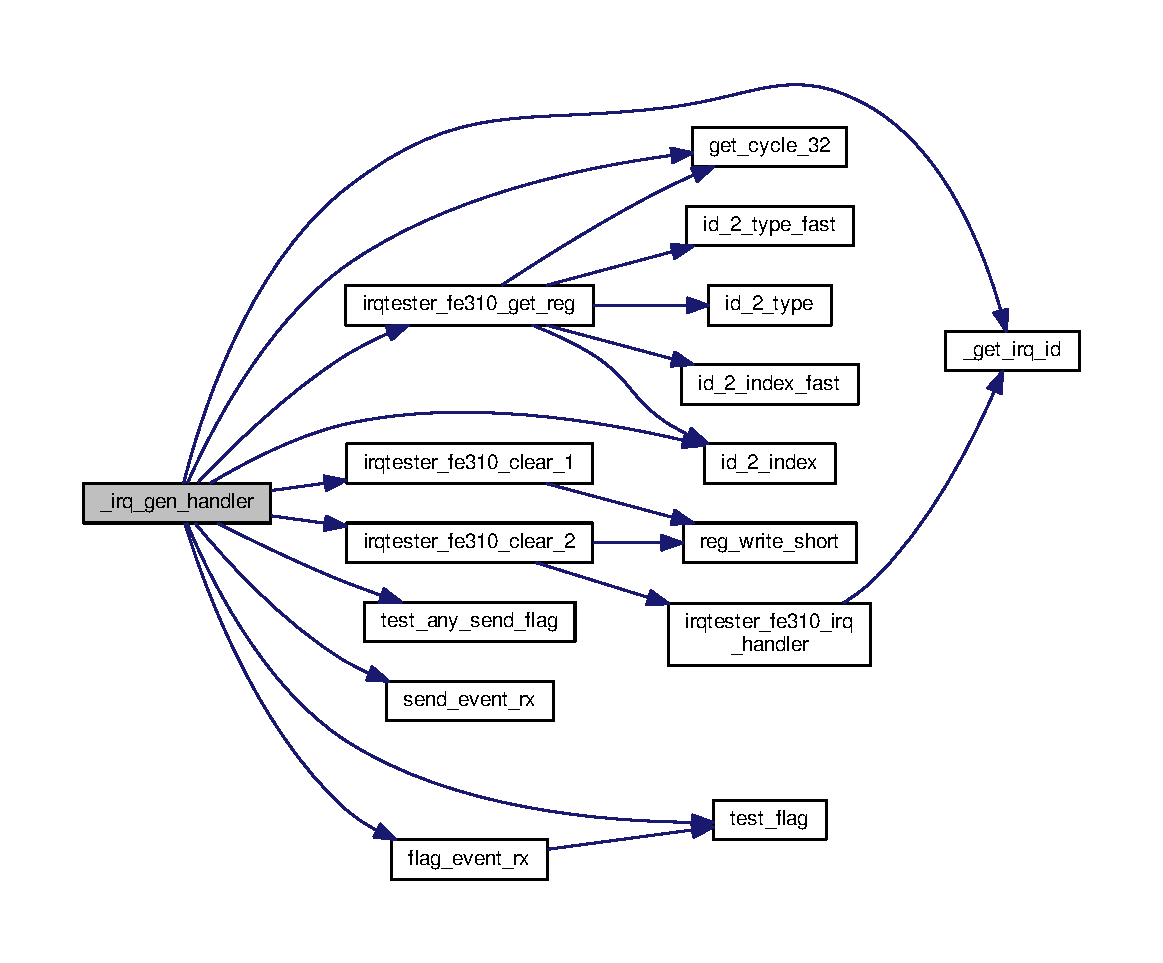
\includegraphics[width=350pt]{irqtestperipheral_8c_a8b6a6dc9fd115e8c6346549531d43199_cgraph}
\end{center}
\end{figure}


\index{irqtestperipheral.\+c@{irqtestperipheral.\+c}!flag\+\_\+event\+\_\+rx@{flag\+\_\+event\+\_\+rx}}
\index{flag\+\_\+event\+\_\+rx@{flag\+\_\+event\+\_\+rx}!irqtestperipheral.\+c@{irqtestperipheral.\+c}}
\subsubsection[{\texorpdfstring{flag\+\_\+event\+\_\+rx(struct device $\ast$dev, struct Drv\+Event $\ast$evt)}{flag_event_rx(struct device *dev, struct DrvEvent *evt)}}]{\setlength{\rightskip}{0pt plus 5cm}static void flag\+\_\+event\+\_\+rx (
\begin{DoxyParamCaption}
\item[{struct device $\ast$}]{dev, }
\item[{struct {\bf Drv\+Event} $\ast$}]{evt}
\end{DoxyParamCaption}
)\hspace{0.3cm}{\ttfamily [inline]}, {\ttfamily [static]}}\hypertarget{irqtestperipheral_8c_a95991437cd831bd6ad077bc6382059ee}{}\label{irqtestperipheral_8c_a95991437cd831bd6ad077bc6382059ee}


Sets the (atomic) flag to indicate to higher level applications that event occured. 

Differs from \hyperlink{irqtestperipheral_8c_aea8fe973b67fd1364c333f4ba595b6db}{send\+\_\+event\+\_\+rx()}. No usage of kernel object for synchronization (eg. queue, semaphore) 

Here is the call graph for this function\+:\nopagebreak
\begin{figure}[H]
\begin{center}
\leavevmode
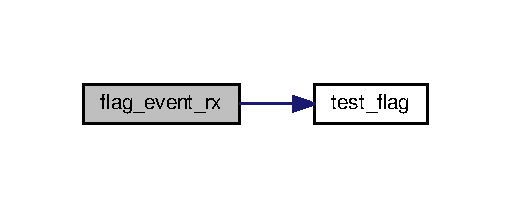
\includegraphics[width=245pt]{irqtestperipheral_8c_a95991437cd831bd6ad077bc6382059ee_cgraph}
\end{center}
\end{figure}


\index{irqtestperipheral.\+c@{irqtestperipheral.\+c}!id\+\_\+2\+\_\+index@{id\+\_\+2\+\_\+index}}
\index{id\+\_\+2\+\_\+index@{id\+\_\+2\+\_\+index}!irqtestperipheral.\+c@{irqtestperipheral.\+c}}
\subsubsection[{\texorpdfstring{id\+\_\+2\+\_\+index(irqt\+\_\+val\+\_\+id\+\_\+t id)}{id_2_index(irqt_val_id_t id)}}]{\setlength{\rightskip}{0pt plus 5cm}static int id\+\_\+2\+\_\+index (
\begin{DoxyParamCaption}
\item[{{\bf irqt\+\_\+val\+\_\+id\+\_\+t}}]{id}
\end{DoxyParamCaption}
)\hspace{0.3cm}{\ttfamily [inline]}, {\ttfamily [static]}}\hypertarget{irqtestperipheral_8c_a3205d750d033a40f72392b0d638b9070}{}\label{irqtestperipheral_8c_a3205d750d033a40f72392b0d638b9070}
\index{irqtestperipheral.\+c@{irqtestperipheral.\+c}!id\+\_\+2\+\_\+index\+\_\+fast@{id\+\_\+2\+\_\+index\+\_\+fast}}
\index{id\+\_\+2\+\_\+index\+\_\+fast@{id\+\_\+2\+\_\+index\+\_\+fast}!irqtestperipheral.\+c@{irqtestperipheral.\+c}}
\subsubsection[{\texorpdfstring{id\+\_\+2\+\_\+index\+\_\+fast(irqt\+\_\+val\+\_\+id\+\_\+t id, irqt\+\_\+val\+\_\+type\+\_\+t type)}{id_2_index_fast(irqt_val_id_t id, irqt_val_type_t type)}}]{\setlength{\rightskip}{0pt plus 5cm}static int id\+\_\+2\+\_\+index\+\_\+fast (
\begin{DoxyParamCaption}
\item[{{\bf irqt\+\_\+val\+\_\+id\+\_\+t}}]{id, }
\item[{{\bf irqt\+\_\+val\+\_\+type\+\_\+t}}]{type}
\end{DoxyParamCaption}
)\hspace{0.3cm}{\ttfamily [inline]}, {\ttfamily [static]}}\hypertarget{irqtestperipheral_8c_aae36b616bf3ffc8134b83f3e168bdf0e}{}\label{irqtestperipheral_8c_aae36b616bf3ffc8134b83f3e168bdf0e}
\index{irqtestperipheral.\+c@{irqtestperipheral.\+c}!id\+\_\+2\+\_\+type@{id\+\_\+2\+\_\+type}}
\index{id\+\_\+2\+\_\+type@{id\+\_\+2\+\_\+type}!irqtestperipheral.\+c@{irqtestperipheral.\+c}}
\subsubsection[{\texorpdfstring{id\+\_\+2\+\_\+type(irqt\+\_\+val\+\_\+id\+\_\+t id)}{id_2_type(irqt_val_id_t id)}}]{\setlength{\rightskip}{0pt plus 5cm}static {\bf irqt\+\_\+val\+\_\+type\+\_\+t} id\+\_\+2\+\_\+type (
\begin{DoxyParamCaption}
\item[{{\bf irqt\+\_\+val\+\_\+id\+\_\+t}}]{id}
\end{DoxyParamCaption}
)\hspace{0.3cm}{\ttfamily [inline]}, {\ttfamily [static]}}\hypertarget{irqtestperipheral_8c_a15420b03ab67124ddc6d1b4f63f32309}{}\label{irqtestperipheral_8c_a15420b03ab67124ddc6d1b4f63f32309}
\index{irqtestperipheral.\+c@{irqtestperipheral.\+c}!id\+\_\+2\+\_\+type\+\_\+fast@{id\+\_\+2\+\_\+type\+\_\+fast}}
\index{id\+\_\+2\+\_\+type\+\_\+fast@{id\+\_\+2\+\_\+type\+\_\+fast}!irqtestperipheral.\+c@{irqtestperipheral.\+c}}
\subsubsection[{\texorpdfstring{id\+\_\+2\+\_\+type\+\_\+fast(irqt\+\_\+val\+\_\+id\+\_\+t id)}{id_2_type_fast(irqt_val_id_t id)}}]{\setlength{\rightskip}{0pt plus 5cm}static {\bf irqt\+\_\+val\+\_\+type\+\_\+t} id\+\_\+2\+\_\+type\+\_\+fast (
\begin{DoxyParamCaption}
\item[{{\bf irqt\+\_\+val\+\_\+id\+\_\+t}}]{id}
\end{DoxyParamCaption}
)\hspace{0.3cm}{\ttfamily [inline]}, {\ttfamily [static]}}\hypertarget{irqtestperipheral_8c_aacd45cbca76d5cb252b111e2e064a3e0}{}\label{irqtestperipheral_8c_aacd45cbca76d5cb252b111e2e064a3e0}
\index{irqtestperipheral.\+c@{irqtestperipheral.\+c}!irqtester\+\_\+fe310\+\_\+clear\+\_\+1@{irqtester\+\_\+fe310\+\_\+clear\+\_\+1}}
\index{irqtester\+\_\+fe310\+\_\+clear\+\_\+1@{irqtester\+\_\+fe310\+\_\+clear\+\_\+1}!irqtestperipheral.\+c@{irqtestperipheral.\+c}}
\subsubsection[{\texorpdfstring{irqtester\+\_\+fe310\+\_\+clear\+\_\+1(struct device $\ast$dev)}{irqtester_fe310_clear_1(struct device *dev)}}]{\setlength{\rightskip}{0pt plus 5cm}void irqtester\+\_\+fe310\+\_\+clear\+\_\+1 (
\begin{DoxyParamCaption}
\item[{struct device $\ast$}]{dev}
\end{DoxyParamCaption}
)}\hypertarget{irqtestperipheral_8c_a260bbaa36d21fbbf0441d4d15fe1a5e0}{}\label{irqtestperipheral_8c_a260bbaa36d21fbbf0441d4d15fe1a5e0}


Here is the call graph for this function\+:\nopagebreak
\begin{figure}[H]
\begin{center}
\leavevmode
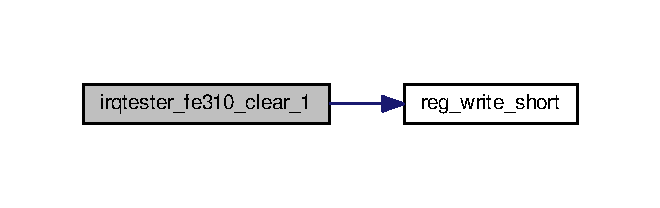
\includegraphics[width=317pt]{irqtestperipheral_8c_a260bbaa36d21fbbf0441d4d15fe1a5e0_cgraph}
\end{center}
\end{figure}


\index{irqtestperipheral.\+c@{irqtestperipheral.\+c}!irqtester\+\_\+fe310\+\_\+clear\+\_\+2@{irqtester\+\_\+fe310\+\_\+clear\+\_\+2}}
\index{irqtester\+\_\+fe310\+\_\+clear\+\_\+2@{irqtester\+\_\+fe310\+\_\+clear\+\_\+2}!irqtestperipheral.\+c@{irqtestperipheral.\+c}}
\subsubsection[{\texorpdfstring{irqtester\+\_\+fe310\+\_\+clear\+\_\+2(struct device $\ast$dev)}{irqtester_fe310_clear_2(struct device *dev)}}]{\setlength{\rightskip}{0pt plus 5cm}void irqtester\+\_\+fe310\+\_\+clear\+\_\+2 (
\begin{DoxyParamCaption}
\item[{struct device $\ast$}]{dev}
\end{DoxyParamCaption}
)}\hypertarget{irqtestperipheral_8c_ac28383949304b588aecac37c6d6ea538}{}\label{irqtestperipheral_8c_ac28383949304b588aecac37c6d6ea538}


Here is the call graph for this function\+:\nopagebreak
\begin{figure}[H]
\begin{center}
\leavevmode
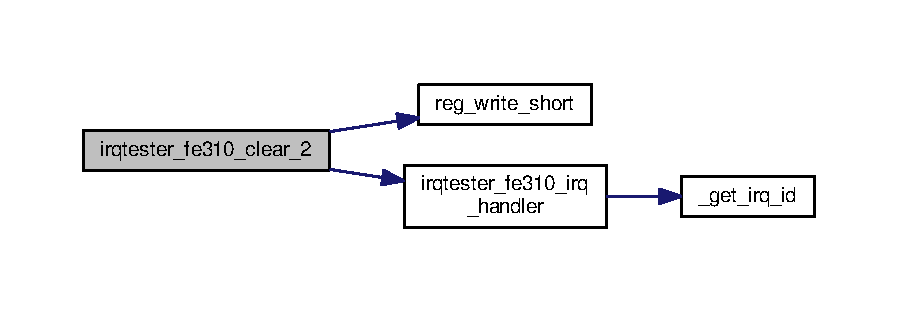
\includegraphics[width=350pt]{irqtestperipheral_8c_ac28383949304b588aecac37c6d6ea538_cgraph}
\end{center}
\end{figure}


\index{irqtestperipheral.\+c@{irqtestperipheral.\+c}!irqtester\+\_\+fe310\+\_\+clear\+\_\+all\+\_\+valflags@{irqtester\+\_\+fe310\+\_\+clear\+\_\+all\+\_\+valflags}}
\index{irqtester\+\_\+fe310\+\_\+clear\+\_\+all\+\_\+valflags@{irqtester\+\_\+fe310\+\_\+clear\+\_\+all\+\_\+valflags}!irqtestperipheral.\+c@{irqtestperipheral.\+c}}
\subsubsection[{\texorpdfstring{irqtester\+\_\+fe310\+\_\+clear\+\_\+all\+\_\+valflags(struct device $\ast$dev)}{irqtester_fe310_clear_all_valflags(struct device *dev)}}]{\setlength{\rightskip}{0pt plus 5cm}void irqtester\+\_\+fe310\+\_\+clear\+\_\+all\+\_\+valflags (
\begin{DoxyParamCaption}
\item[{struct device $\ast$}]{dev}
\end{DoxyParamCaption}
)}\hypertarget{irqtestperipheral_8c_a997c5939bc6f47d246540c69ff49733d}{}\label{irqtestperipheral_8c_a997c5939bc6f47d246540c69ff49733d}


Clear all flags. 

\index{irqtestperipheral.\+c@{irqtestperipheral.\+c}!irqtester\+\_\+fe310\+\_\+dbgprint\+\_\+event@{irqtester\+\_\+fe310\+\_\+dbgprint\+\_\+event}}
\index{irqtester\+\_\+fe310\+\_\+dbgprint\+\_\+event@{irqtester\+\_\+fe310\+\_\+dbgprint\+\_\+event}!irqtestperipheral.\+c@{irqtestperipheral.\+c}}
\subsubsection[{\texorpdfstring{irqtester\+\_\+fe310\+\_\+dbgprint\+\_\+event(struct device $\ast$dev, struct Drv\+Event $\ast$evt)}{irqtester_fe310_dbgprint_event(struct device *dev, struct DrvEvent *evt)}}]{\setlength{\rightskip}{0pt plus 5cm}void irqtester\+\_\+fe310\+\_\+dbgprint\+\_\+event (
\begin{DoxyParamCaption}
\item[{struct device $\ast$}]{dev, }
\item[{struct {\bf Drv\+Event} $\ast$}]{evt}
\end{DoxyParamCaption}
)}\hypertarget{irqtestperipheral_8c_ae5817f51846271d1228fa02cc0e1726e}{}\label{irqtestperipheral_8c_ae5817f51846271d1228fa02cc0e1726e}


Print information about an event as a debug log message. 



Here is the call graph for this function\+:\nopagebreak
\begin{figure}[H]
\begin{center}
\leavevmode
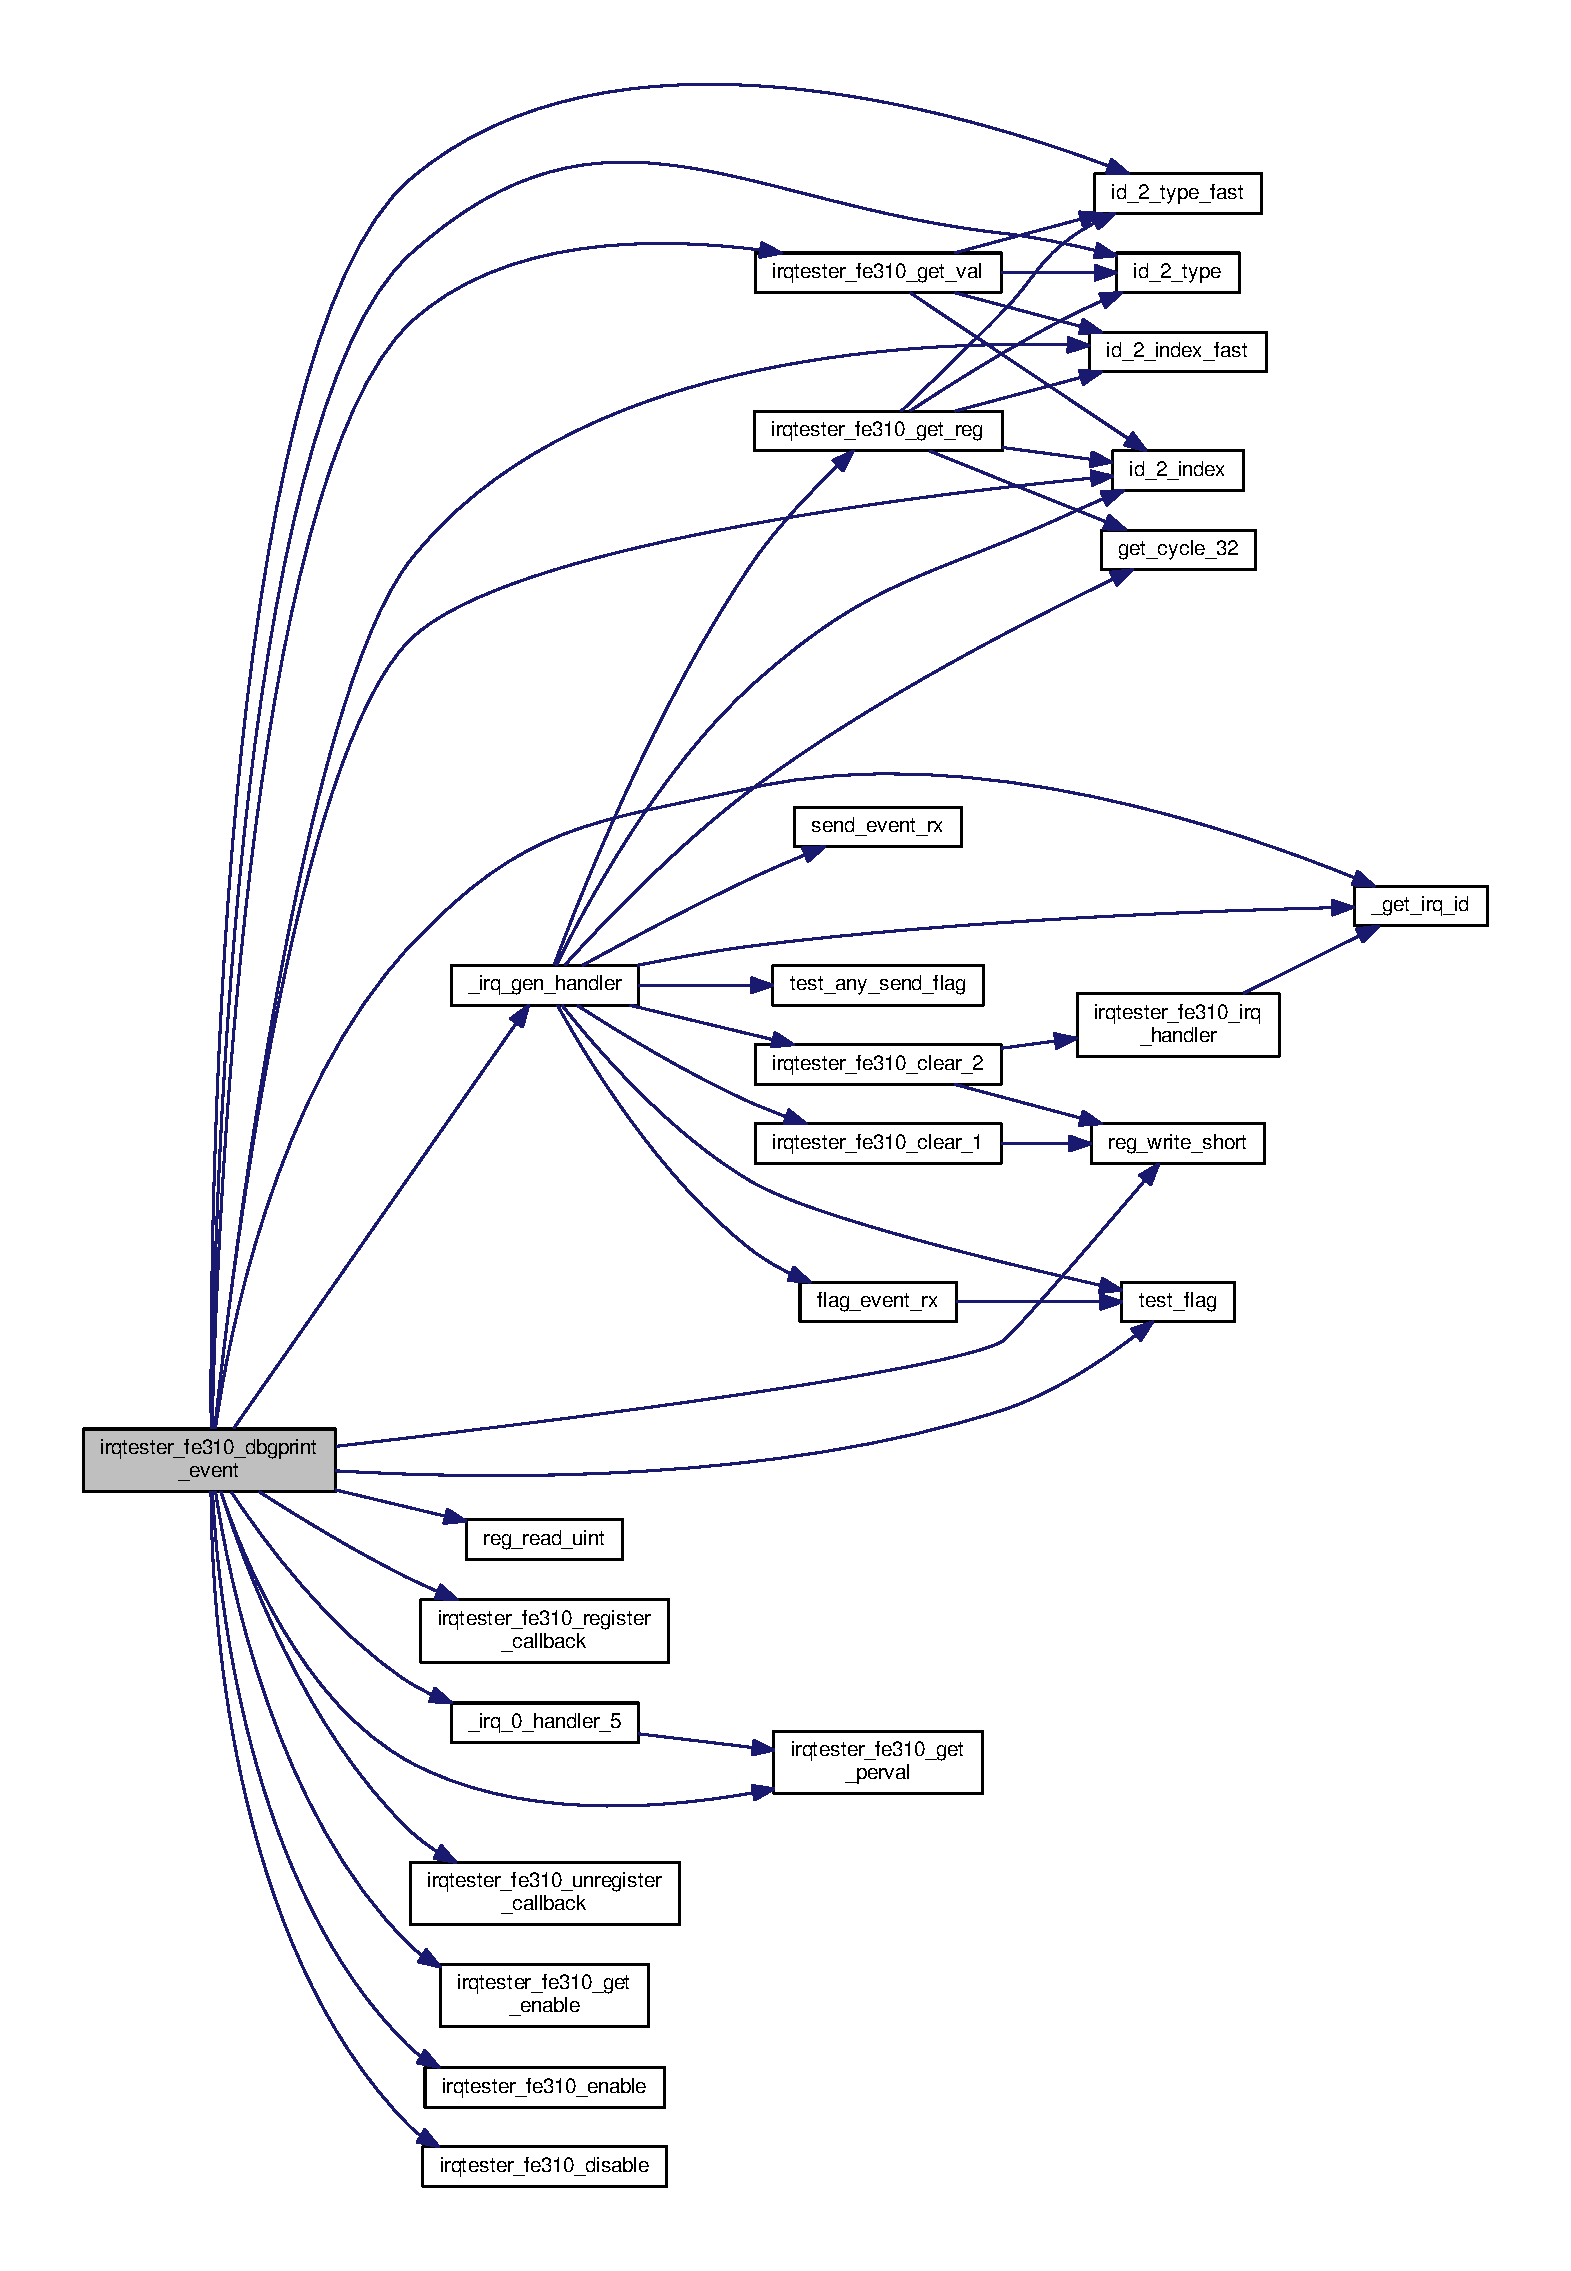
\includegraphics[width=350pt]{irqtestperipheral_8c_ae5817f51846271d1228fa02cc0e1726e_cgraph}
\end{center}
\end{figure}


\index{irqtestperipheral.\+c@{irqtestperipheral.\+c}!irqtester\+\_\+fe310\+\_\+enable\+\_\+fifo\+\_\+rx@{irqtester\+\_\+fe310\+\_\+enable\+\_\+fifo\+\_\+rx}}
\index{irqtester\+\_\+fe310\+\_\+enable\+\_\+fifo\+\_\+rx@{irqtester\+\_\+fe310\+\_\+enable\+\_\+fifo\+\_\+rx}!irqtestperipheral.\+c@{irqtestperipheral.\+c}}
\subsubsection[{\texorpdfstring{irqtester\+\_\+fe310\+\_\+enable\+\_\+fifo\+\_\+rx(struct device $\ast$dev)}{irqtester_fe310_enable_fifo_rx(struct device *dev)}}]{\setlength{\rightskip}{0pt plus 5cm}int irqtester\+\_\+fe310\+\_\+enable\+\_\+fifo\+\_\+rx (
\begin{DoxyParamCaption}
\item[{struct device $\ast$}]{dev}
\end{DoxyParamCaption}
)}\hypertarget{irqtestperipheral_8c_aff89ef81c09b5a1c7631fc236b671e7d}{}\label{irqtestperipheral_8c_aff89ef81c09b5a1c7631fc236b671e7d}


Enable previously registered fifo\+\_\+rx for sending driver events to. 



Here is the call graph for this function\+:\nopagebreak
\begin{figure}[H]
\begin{center}
\leavevmode
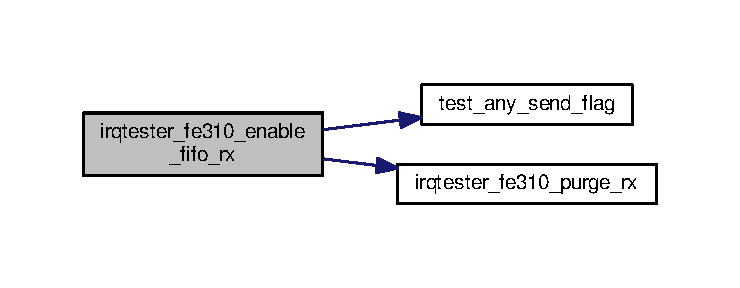
\includegraphics[width=350pt]{irqtestperipheral_8c_aff89ef81c09b5a1c7631fc236b671e7d_cgraph}
\end{center}
\end{figure}


\index{irqtestperipheral.\+c@{irqtestperipheral.\+c}!irqtester\+\_\+fe310\+\_\+enable\+\_\+queue\+\_\+rx@{irqtester\+\_\+fe310\+\_\+enable\+\_\+queue\+\_\+rx}}
\index{irqtester\+\_\+fe310\+\_\+enable\+\_\+queue\+\_\+rx@{irqtester\+\_\+fe310\+\_\+enable\+\_\+queue\+\_\+rx}!irqtestperipheral.\+c@{irqtestperipheral.\+c}}
\subsubsection[{\texorpdfstring{irqtester\+\_\+fe310\+\_\+enable\+\_\+queue\+\_\+rx(struct device $\ast$dev)}{irqtester_fe310_enable_queue_rx(struct device *dev)}}]{\setlength{\rightskip}{0pt plus 5cm}int irqtester\+\_\+fe310\+\_\+enable\+\_\+queue\+\_\+rx (
\begin{DoxyParamCaption}
\item[{struct device $\ast$}]{dev}
\end{DoxyParamCaption}
)}\hypertarget{irqtestperipheral_8c_a9c8c75c9c4603bdccd5bdcf3038d3c49}{}\label{irqtestperipheral_8c_a9c8c75c9c4603bdccd5bdcf3038d3c49}


Enable previously registered queue\+\_\+rx for sending driver events to. 



Here is the call graph for this function\+:\nopagebreak
\begin{figure}[H]
\begin{center}
\leavevmode
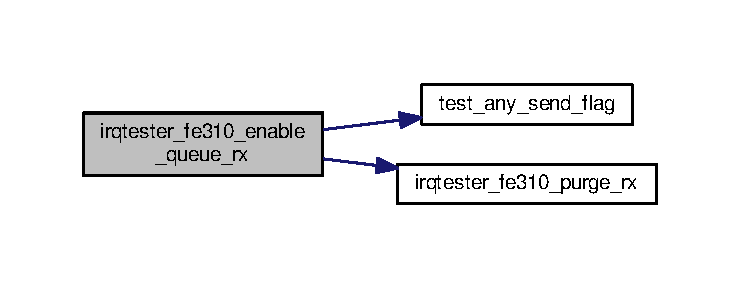
\includegraphics[width=350pt]{irqtestperipheral_8c_a9c8c75c9c4603bdccd5bdcf3038d3c49_cgraph}
\end{center}
\end{figure}


\index{irqtestperipheral.\+c@{irqtestperipheral.\+c}!irqtester\+\_\+fe310\+\_\+enable\+\_\+sem\+\_\+arr\+\_\+rx@{irqtester\+\_\+fe310\+\_\+enable\+\_\+sem\+\_\+arr\+\_\+rx}}
\index{irqtester\+\_\+fe310\+\_\+enable\+\_\+sem\+\_\+arr\+\_\+rx@{irqtester\+\_\+fe310\+\_\+enable\+\_\+sem\+\_\+arr\+\_\+rx}!irqtestperipheral.\+c@{irqtestperipheral.\+c}}
\subsubsection[{\texorpdfstring{irqtester\+\_\+fe310\+\_\+enable\+\_\+sem\+\_\+arr\+\_\+rx(struct device $\ast$dev)}{irqtester_fe310_enable_sem_arr_rx(struct device *dev)}}]{\setlength{\rightskip}{0pt plus 5cm}int irqtester\+\_\+fe310\+\_\+enable\+\_\+sem\+\_\+arr\+\_\+rx (
\begin{DoxyParamCaption}
\item[{struct device $\ast$}]{dev}
\end{DoxyParamCaption}
)}\hypertarget{irqtestperipheral_8c_acc15d23902deee0d82e20e237a526275}{}\label{irqtestperipheral_8c_acc15d23902deee0d82e20e237a526275}


Enable previously registered semaphore plus event array for sending driver events to. 



Here is the call graph for this function\+:\nopagebreak
\begin{figure}[H]
\begin{center}
\leavevmode
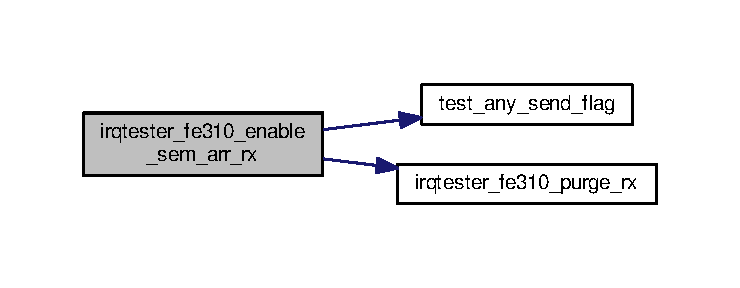
\includegraphics[width=350pt]{irqtestperipheral_8c_acc15d23902deee0d82e20e237a526275_cgraph}
\end{center}
\end{figure}


\index{irqtestperipheral.\+c@{irqtestperipheral.\+c}!irqtester\+\_\+fe310\+\_\+enable\+\_\+valflags\+\_\+rx@{irqtester\+\_\+fe310\+\_\+enable\+\_\+valflags\+\_\+rx}}
\index{irqtester\+\_\+fe310\+\_\+enable\+\_\+valflags\+\_\+rx@{irqtester\+\_\+fe310\+\_\+enable\+\_\+valflags\+\_\+rx}!irqtestperipheral.\+c@{irqtestperipheral.\+c}}
\subsubsection[{\texorpdfstring{irqtester\+\_\+fe310\+\_\+enable\+\_\+valflags\+\_\+rx(struct device $\ast$dev)}{irqtester_fe310_enable_valflags_rx(struct device *dev)}}]{\setlength{\rightskip}{0pt plus 5cm}int irqtester\+\_\+fe310\+\_\+enable\+\_\+valflags\+\_\+rx (
\begin{DoxyParamCaption}
\item[{struct device $\ast$}]{dev}
\end{DoxyParamCaption}
)}\hypertarget{irqtestperipheral_8c_ace5f0827eb25f735e652ab09f4cbe3b2}{}\label{irqtestperipheral_8c_ace5f0827eb25f735e652ab09f4cbe3b2}


Enables flags for indicating load of harware values to driver memory. 

Since they don\textquotesingle{}t issue events, valflags can be enabled in parallel to other sending flags which do issue events. \index{irqtestperipheral.\+c@{irqtestperipheral.\+c}!irqtester\+\_\+fe310\+\_\+fire@{irqtester\+\_\+fe310\+\_\+fire}}
\index{irqtester\+\_\+fe310\+\_\+fire@{irqtester\+\_\+fe310\+\_\+fire}!irqtestperipheral.\+c@{irqtestperipheral.\+c}}
\subsubsection[{\texorpdfstring{irqtester\+\_\+fe310\+\_\+fire(struct device $\ast$dev)}{irqtester_fe310_fire(struct device *dev)}}]{\setlength{\rightskip}{0pt plus 5cm}int irqtester\+\_\+fe310\+\_\+fire (
\begin{DoxyParamCaption}
\item[{struct device $\ast$}]{dev}
\end{DoxyParamCaption}
)}\hypertarget{irqtestperipheral_8c_ac1e81dcf0faf4348a6121675f46553ff}{}\label{irqtestperipheral_8c_ac1e81dcf0faf4348a6121675f46553ff}
\index{irqtestperipheral.\+c@{irqtestperipheral.\+c}!irqtester\+\_\+fe310\+\_\+fire\+\_\+1@{irqtester\+\_\+fe310\+\_\+fire\+\_\+1}}
\index{irqtester\+\_\+fe310\+\_\+fire\+\_\+1@{irqtester\+\_\+fe310\+\_\+fire\+\_\+1}!irqtestperipheral.\+c@{irqtestperipheral.\+c}}
\subsubsection[{\texorpdfstring{irqtester\+\_\+fe310\+\_\+fire\+\_\+1(struct device $\ast$dev)}{irqtester_fe310_fire_1(struct device *dev)}}]{\setlength{\rightskip}{0pt plus 5cm}void irqtester\+\_\+fe310\+\_\+fire\+\_\+1 (
\begin{DoxyParamCaption}
\item[{struct device $\ast$}]{dev}
\end{DoxyParamCaption}
)}\hypertarget{irqtestperipheral_8c_a0bd81b8a8b0a9eb85658ffcfe6c0a7e5}{}\label{irqtestperipheral_8c_a0bd81b8a8b0a9eb85658ffcfe6c0a7e5}


Need to set regs num\+\_\+rep\+\_\+1 and period\+\_\+1 first. 

\index{irqtestperipheral.\+c@{irqtestperipheral.\+c}!irqtester\+\_\+fe310\+\_\+fire\+\_\+2@{irqtester\+\_\+fe310\+\_\+fire\+\_\+2}}
\index{irqtester\+\_\+fe310\+\_\+fire\+\_\+2@{irqtester\+\_\+fe310\+\_\+fire\+\_\+2}!irqtestperipheral.\+c@{irqtestperipheral.\+c}}
\subsubsection[{\texorpdfstring{irqtester\+\_\+fe310\+\_\+fire\+\_\+2(struct device $\ast$dev)}{irqtester_fe310_fire_2(struct device *dev)}}]{\setlength{\rightskip}{0pt plus 5cm}int irqtester\+\_\+fe310\+\_\+fire\+\_\+2 (
\begin{DoxyParamCaption}
\item[{struct device $\ast$}]{dev}
\end{DoxyParamCaption}
)}\hypertarget{irqtestperipheral_8c_a3f0daddddbc00ed4d3195cd85ba1acae}{}\label{irqtestperipheral_8c_a3f0daddddbc00ed4d3195cd85ba1acae}


Need to set regs num\+\_\+rep\+\_\+2 and period\+\_\+2 first. 

\index{irqtestperipheral.\+c@{irqtestperipheral.\+c}!irqtester\+\_\+fe310\+\_\+get\+\_\+reg@{irqtester\+\_\+fe310\+\_\+get\+\_\+reg}}
\index{irqtester\+\_\+fe310\+\_\+get\+\_\+reg@{irqtester\+\_\+fe310\+\_\+get\+\_\+reg}!irqtestperipheral.\+c@{irqtestperipheral.\+c}}
\subsubsection[{\texorpdfstring{irqtester\+\_\+fe310\+\_\+get\+\_\+reg(struct device $\ast$dev, irqt\+\_\+val\+\_\+id\+\_\+t id, void $\ast$res\+\_\+val)}{irqtester_fe310_get_reg(struct device *dev, irqt_val_id_t id, void *res_val)}}]{\setlength{\rightskip}{0pt plus 5cm}int irqtester\+\_\+fe310\+\_\+get\+\_\+reg (
\begin{DoxyParamCaption}
\item[{struct device $\ast$}]{dev, }
\item[{{\bf irqt\+\_\+val\+\_\+id\+\_\+t}}]{id, }
\item[{void $\ast$}]{res\+\_\+val}
\end{DoxyParamCaption}
)}\hypertarget{irqtestperipheral_8c_a987670a27b50999e651f384e6b04e582}{}\label{irqtestperipheral_8c_a987670a27b50999e651f384e6b04e582}


Non-\/thread safe, generic getter for device (output) registers. Only works for regs which are loaded to driver mem pools. 

Might be called from an I\+SR, but potentially slower than direct getters. For an reg to be available, \+\_\+store\+\_\+reg\+\_\+addr() has to be called in driver init. 
\begin{DoxyParams}{Parameters}
{\em id} & id of value to set \\
\hline
{\em set\+\_\+value} & pointer to a Drv\+Value\+\_\+X struct of correct type. \\
\hline
\end{DoxyParams}


Here is the call graph for this function\+:\nopagebreak
\begin{figure}[H]
\begin{center}
\leavevmode
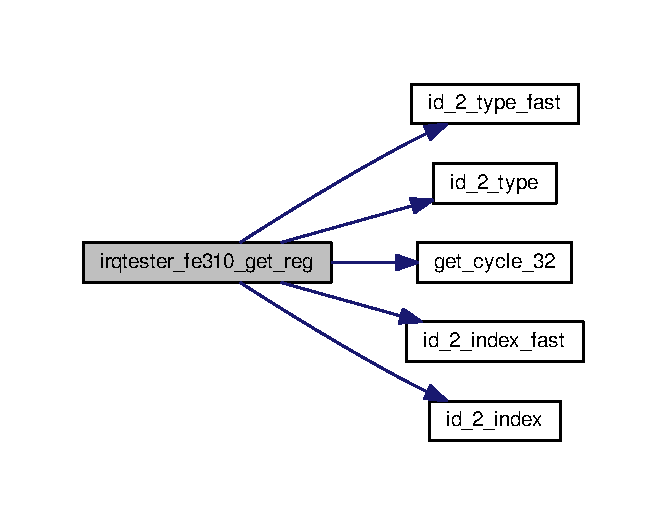
\includegraphics[width=320pt]{irqtestperipheral_8c_a987670a27b50999e651f384e6b04e582_cgraph}
\end{center}
\end{figure}


\index{irqtestperipheral.\+c@{irqtestperipheral.\+c}!irqtester\+\_\+fe310\+\_\+get\+\_\+val@{irqtester\+\_\+fe310\+\_\+get\+\_\+val}}
\index{irqtester\+\_\+fe310\+\_\+get\+\_\+val@{irqtester\+\_\+fe310\+\_\+get\+\_\+val}!irqtestperipheral.\+c@{irqtestperipheral.\+c}}
\subsubsection[{\texorpdfstring{irqtester\+\_\+fe310\+\_\+get\+\_\+val(irqt\+\_\+val\+\_\+id\+\_\+t id, void $\ast$res\+\_\+value)}{irqtester_fe310_get_val(irqt_val_id_t id, void *res_value)}}]{\setlength{\rightskip}{0pt plus 5cm}int irqtester\+\_\+fe310\+\_\+get\+\_\+val (
\begin{DoxyParamCaption}
\item[{{\bf irqt\+\_\+val\+\_\+id\+\_\+t}}]{id, }
\item[{void $\ast$}]{res\+\_\+value}
\end{DoxyParamCaption}
)}\hypertarget{irqtestperipheral_8c_a46f10c3e9b63404c15f52ab375a28977}{}\label{irqtestperipheral_8c_a46f10c3e9b63404c15f52ab375a28977}


Thread safe generic (by id) getter for values of generic type from driver memory pools. 

Doesn\textquotesingle{}t read from registers; an irq is needed to load regs into driver mem. 
\begin{DoxyParams}{Parameters}
{\em id} & id of value to get \\
\hline
{\em res\+\_\+value} & pointer to a Drv\+Value\+\_\+X struct of correct type. \\
\hline
{\em success} & 0, 1 on unknown val\+\_\+type\+\_\+id \\
\hline
\end{DoxyParams}


Here is the call graph for this function\+:\nopagebreak
\begin{figure}[H]
\begin{center}
\leavevmode
\includegraphics[width=319pt]{irqtestperipheral_8c_a46f10c3e9b63404c15f52ab375a28977_cgraph}
\end{center}
\end{figure}


\index{irqtestperipheral.\+c@{irqtestperipheral.\+c}!irqtester\+\_\+fe310\+\_\+get\+\_\+val\+\_\+uint@{irqtester\+\_\+fe310\+\_\+get\+\_\+val\+\_\+uint}}
\index{irqtester\+\_\+fe310\+\_\+get\+\_\+val\+\_\+uint@{irqtester\+\_\+fe310\+\_\+get\+\_\+val\+\_\+uint}!irqtestperipheral.\+c@{irqtestperipheral.\+c}}
\subsubsection[{\texorpdfstring{irqtester\+\_\+fe310\+\_\+get\+\_\+val\+\_\+uint(irqt\+\_\+val\+\_\+id\+\_\+t id, void $\ast$res\+\_\+value)}{irqtester_fe310_get_val_uint(irqt_val_id_t id, void *res_value)}}]{\setlength{\rightskip}{0pt plus 5cm}int irqtester\+\_\+fe310\+\_\+get\+\_\+val\+\_\+uint (
\begin{DoxyParamCaption}
\item[{{\bf irqt\+\_\+val\+\_\+id\+\_\+t}}]{id, }
\item[{void $\ast$}]{res\+\_\+value}
\end{DoxyParamCaption}
)}\hypertarget{irqtestperipheral_8c_a4e987f34af28aea872408b2412339ad7}{}\label{irqtestperipheral_8c_a4e987f34af28aea872408b2412339ad7}


Thread safe generic (by id) getter for values of uint type from driver memory pools. 

Doesn\textquotesingle{}t read from registers; an irq is needed to load regs into driver mem.


\begin{DoxyParams}{Parameters}
{\em id} & id of value to get \\
\hline
{\em res\+\_\+value} & pointer to a \hyperlink{struct_drv_value__uint}{Drv\+Value\+\_\+uint} struct. \\
\hline
\end{DoxyParams}
\begin{DoxyReturn}{Returns}
always 0 
\end{DoxyReturn}


Here is the call graph for this function\+:\nopagebreak
\begin{figure}[H]
\begin{center}
\leavevmode
\includegraphics[width=301pt]{irqtestperipheral_8c_a4e987f34af28aea872408b2412339ad7_cgraph}
\end{center}
\end{figure}


\index{irqtestperipheral.\+c@{irqtestperipheral.\+c}!irqtester\+\_\+fe310\+\_\+get\+\_\+val\+\_\+uint\+\_\+raw@{irqtester\+\_\+fe310\+\_\+get\+\_\+val\+\_\+uint\+\_\+raw}}
\index{irqtester\+\_\+fe310\+\_\+get\+\_\+val\+\_\+uint\+\_\+raw@{irqtester\+\_\+fe310\+\_\+get\+\_\+val\+\_\+uint\+\_\+raw}!irqtestperipheral.\+c@{irqtestperipheral.\+c}}
\subsubsection[{\texorpdfstring{irqtester\+\_\+fe310\+\_\+get\+\_\+val\+\_\+uint\+\_\+raw(irqt\+\_\+val\+\_\+id\+\_\+t id)}{irqtester_fe310_get_val_uint_raw(irqt_val_id_t id)}}]{\setlength{\rightskip}{0pt plus 5cm}u32\+\_\+t irqtester\+\_\+fe310\+\_\+get\+\_\+val\+\_\+uint\+\_\+raw (
\begin{DoxyParamCaption}
\item[{{\bf irqt\+\_\+val\+\_\+id\+\_\+t}}]{id}
\end{DoxyParamCaption}
)}\hypertarget{irqtestperipheral_8c_a2033394f5344ffe1c16f65be91851217}{}\label{irqtestperipheral_8c_a2033394f5344ffe1c16f65be91851217}


Thread safe generic (by id) getter for values of uint type from driver memory pools. For perforamnce reasons, use return value instread a passed container for result. 

Doesn\textquotesingle{}t read from registers; an irq is needed to load regs into driver mem. 
\begin{DoxyParams}{Parameters}
{\em id} & id of value to get \\
\hline
{\em res\+\_\+value} & pointer to a \hyperlink{struct_drv_value__uint}{Drv\+Value\+\_\+uint} struct. \\
\hline
{\em always} & 0 \\
\hline
\end{DoxyParams}


Here is the call graph for this function\+:\nopagebreak
\begin{figure}[H]
\begin{center}
\leavevmode
\includegraphics[width=301pt]{irqtestperipheral_8c_a2033394f5344ffe1c16f65be91851217_cgraph}
\end{center}
\end{figure}


\index{irqtestperipheral.\+c@{irqtestperipheral.\+c}!irqtester\+\_\+fe310\+\_\+irq\+\_\+handler@{irqtester\+\_\+fe310\+\_\+irq\+\_\+handler}}
\index{irqtester\+\_\+fe310\+\_\+irq\+\_\+handler@{irqtester\+\_\+fe310\+\_\+irq\+\_\+handler}!irqtestperipheral.\+c@{irqtestperipheral.\+c}}
\subsubsection[{\texorpdfstring{irqtester\+\_\+fe310\+\_\+irq\+\_\+handler(void $\ast$arg)}{irqtester_fe310_irq_handler(void *arg)}}]{\setlength{\rightskip}{0pt plus 5cm}static void irqtester\+\_\+fe310\+\_\+irq\+\_\+handler (
\begin{DoxyParamCaption}
\item[{void $\ast$}]{arg}
\end{DoxyParamCaption}
)\hspace{0.3cm}{\ttfamily [static]}}\hypertarget{irqtestperipheral_8c_ab157fe508c290d5e05fc878db1c936f0}{}\label{irqtestperipheral_8c_ab157fe508c290d5e05fc878db1c936f0}
I\+RQ Handler registered to the kernel, just calls a callback.


\begin{DoxyParams}{Parameters}
{\em arg} & When kernel calls, this is a handle to the device. \\
\hline
\end{DoxyParams}


Here is the call graph for this function\+:\nopagebreak
\begin{figure}[H]
\begin{center}
\leavevmode
\includegraphics[width=277pt]{irqtestperipheral_8c_ab157fe508c290d5e05fc878db1c936f0_cgraph}
\end{center}
\end{figure}


\index{irqtestperipheral.\+c@{irqtestperipheral.\+c}!irqtester\+\_\+fe310\+\_\+purge\+\_\+rx@{irqtester\+\_\+fe310\+\_\+purge\+\_\+rx}}
\index{irqtester\+\_\+fe310\+\_\+purge\+\_\+rx@{irqtester\+\_\+fe310\+\_\+purge\+\_\+rx}!irqtestperipheral.\+c@{irqtestperipheral.\+c}}
\subsubsection[{\texorpdfstring{irqtester\+\_\+fe310\+\_\+purge\+\_\+rx(struct device $\ast$dev)}{irqtester_fe310_purge_rx(struct device *dev)}}]{\setlength{\rightskip}{0pt plus 5cm}int irqtester\+\_\+fe310\+\_\+purge\+\_\+rx (
\begin{DoxyParamCaption}
\item[{struct device $\ast$}]{dev}
\end{DoxyParamCaption}
)}\hypertarget{irqtestperipheral_8c_ab47c9b38275ed5cb45931e907725dc06}{}\label{irqtestperipheral_8c_ab47c9b38275ed5cb45931e907725dc06}


Reset all objects related to receiving data from this driver. 

\index{irqtestperipheral.\+c@{irqtestperipheral.\+c}!irqtester\+\_\+fe310\+\_\+receive\+\_\+evt\+\_\+from\+\_\+arr@{irqtester\+\_\+fe310\+\_\+receive\+\_\+evt\+\_\+from\+\_\+arr}}
\index{irqtester\+\_\+fe310\+\_\+receive\+\_\+evt\+\_\+from\+\_\+arr@{irqtester\+\_\+fe310\+\_\+receive\+\_\+evt\+\_\+from\+\_\+arr}!irqtestperipheral.\+c@{irqtestperipheral.\+c}}
\subsubsection[{\texorpdfstring{irqtester\+\_\+fe310\+\_\+receive\+\_\+evt\+\_\+from\+\_\+arr(struct device $\ast$dev, struct Drv\+Event $\ast$res, s32\+\_\+t timeout)}{irqtester_fe310_receive_evt_from_arr(struct device *dev, struct DrvEvent *res, s32_t timeout)}}]{\setlength{\rightskip}{0pt plus 5cm}int irqtester\+\_\+fe310\+\_\+receive\+\_\+evt\+\_\+from\+\_\+arr (
\begin{DoxyParamCaption}
\item[{struct device $\ast$}]{dev, }
\item[{struct {\bf Drv\+Event} $\ast$}]{res, }
\item[{s32\+\_\+t}]{timeout}
\end{DoxyParamCaption}
)}\hypertarget{irqtestperipheral_8c_a254eae890ba510e5e473a046407ba618}{}\label{irqtestperipheral_8c_a254eae890ba510e5e473a046407ba618}


If using semaphore plus event array, call this to wait and receive an event. 

Should be called from a single thread only. Todo\+: add example for usage \index{irqtestperipheral.\+c@{irqtestperipheral.\+c}!irqtester\+\_\+fe310\+\_\+register\+\_\+fifo\+\_\+rx@{irqtester\+\_\+fe310\+\_\+register\+\_\+fifo\+\_\+rx}}
\index{irqtester\+\_\+fe310\+\_\+register\+\_\+fifo\+\_\+rx@{irqtester\+\_\+fe310\+\_\+register\+\_\+fifo\+\_\+rx}!irqtestperipheral.\+c@{irqtestperipheral.\+c}}
\subsubsection[{\texorpdfstring{irqtester\+\_\+fe310\+\_\+register\+\_\+fifo\+\_\+rx(struct device $\ast$dev, struct k\+\_\+fifo $\ast$queue)}{irqtester_fe310_register_fifo_rx(struct device *dev, struct k_fifo *queue)}}]{\setlength{\rightskip}{0pt plus 5cm}int irqtester\+\_\+fe310\+\_\+register\+\_\+fifo\+\_\+rx (
\begin{DoxyParamCaption}
\item[{struct device $\ast$}]{dev, }
\item[{struct k\+\_\+fifo $\ast$}]{queue}
\end{DoxyParamCaption}
)}\hypertarget{irqtestperipheral_8c_ace3a40543bbebb04e1324fbfa9f60275}{}\label{irqtestperipheral_8c_ace3a40543bbebb04e1324fbfa9f60275}


Provide a handle to a fifo to receive msgs from the driver there. 

Remember to enable\+\_\+fifo\+\_\+rx() and to empty it in the consuming thread. Attention\+: Using a fifo is not recommended, as it is not necessarily faster and prone to causing overflows (unlimited size!). \index{irqtestperipheral.\+c@{irqtestperipheral.\+c}!irqtester\+\_\+fe310\+\_\+register\+\_\+queue\+\_\+rx@{irqtester\+\_\+fe310\+\_\+register\+\_\+queue\+\_\+rx}}
\index{irqtester\+\_\+fe310\+\_\+register\+\_\+queue\+\_\+rx@{irqtester\+\_\+fe310\+\_\+register\+\_\+queue\+\_\+rx}!irqtestperipheral.\+c@{irqtestperipheral.\+c}}
\subsubsection[{\texorpdfstring{irqtester\+\_\+fe310\+\_\+register\+\_\+queue\+\_\+rx(struct device $\ast$dev, struct k\+\_\+msgq $\ast$queue)}{irqtester_fe310_register_queue_rx(struct device *dev, struct k_msgq *queue)}}]{\setlength{\rightskip}{0pt plus 5cm}int irqtester\+\_\+fe310\+\_\+register\+\_\+queue\+\_\+rx (
\begin{DoxyParamCaption}
\item[{struct device $\ast$}]{dev, }
\item[{struct k\+\_\+msgq $\ast$}]{queue}
\end{DoxyParamCaption}
)}\hypertarget{irqtestperipheral_8c_a8b03f7c9aff5996a16845f0e2d1e6937}{}\label{irqtestperipheral_8c_a8b03f7c9aff5996a16845f0e2d1e6937}


Provide a handle to a queue to receive msgs from the driver there. 

Remember to enable\+\_\+queue\+\_\+rx() and to empty it in the consuming thread. 
\begin{DoxyParams}{Parameters}
{\em k\+\_\+msgsq} & pointer to queue \\
\hline
\end{DoxyParams}
\index{irqtestperipheral.\+c@{irqtestperipheral.\+c}!irqtester\+\_\+fe310\+\_\+register\+\_\+sem\+\_\+arr\+\_\+rx@{irqtester\+\_\+fe310\+\_\+register\+\_\+sem\+\_\+arr\+\_\+rx}}
\index{irqtester\+\_\+fe310\+\_\+register\+\_\+sem\+\_\+arr\+\_\+rx@{irqtester\+\_\+fe310\+\_\+register\+\_\+sem\+\_\+arr\+\_\+rx}!irqtestperipheral.\+c@{irqtestperipheral.\+c}}
\subsubsection[{\texorpdfstring{irqtester\+\_\+fe310\+\_\+register\+\_\+sem\+\_\+arr\+\_\+rx(struct device $\ast$dev, struct k\+\_\+sem $\ast$sem, struct Drv\+Event evt\+\_\+arr[], int len)}{irqtester_fe310_register_sem_arr_rx(struct device *dev, struct k_sem *sem, struct DrvEvent evt_arr[], int len)}}]{\setlength{\rightskip}{0pt plus 5cm}int irqtester\+\_\+fe310\+\_\+register\+\_\+sem\+\_\+arr\+\_\+rx (
\begin{DoxyParamCaption}
\item[{struct device $\ast$}]{dev, }
\item[{struct k\+\_\+sem $\ast$}]{sem, }
\item[{struct {\bf Drv\+Event}}]{evt\+\_\+arr\mbox{[}$\,$\mbox{]}, }
\item[{int}]{len}
\end{DoxyParamCaption}
)}\hypertarget{irqtestperipheral_8c_ae82ab1a2ea6ec7bd8f6b43530d1419a5}{}\label{irqtestperipheral_8c_ae82ab1a2ea6ec7bd8f6b43530d1419a5}


Provide a handle to a semaphore and an even array to receive msgs from the driver there. 

Remember to enable\+\_\+fifo\+\_\+rx() and to empty it in the consuming thread. \index{irqtestperipheral.\+c@{irqtestperipheral.\+c}!irqtester\+\_\+fe310\+\_\+reset\+\_\+hw@{irqtester\+\_\+fe310\+\_\+reset\+\_\+hw}}
\index{irqtester\+\_\+fe310\+\_\+reset\+\_\+hw@{irqtester\+\_\+fe310\+\_\+reset\+\_\+hw}!irqtestperipheral.\+c@{irqtestperipheral.\+c}}
\subsubsection[{\texorpdfstring{irqtester\+\_\+fe310\+\_\+reset\+\_\+hw(struct device $\ast$dev)}{irqtester_fe310_reset_hw(struct device *dev)}}]{\setlength{\rightskip}{0pt plus 5cm}int irqtester\+\_\+fe310\+\_\+reset\+\_\+hw (
\begin{DoxyParamCaption}
\item[{struct device $\ast$}]{dev}
\end{DoxyParamCaption}
)}\hypertarget{irqtestperipheral_8c_a1d2af0fa1a30580646c700e462bf063f}{}\label{irqtestperipheral_8c_a1d2af0fa1a30580646c700e462bf063f}


Reset all hw regs but \textquotesingle{}enable\textquotesingle{} to 0. Doesn\textquotesingle{}t reset internal and output regs! 


\begin{DoxyParams}{Parameters}
{\em dev} & I\+R\+Q\+Tester device struct\\
\hline
\end{DoxyParams}
\begin{DoxyReturn}{Returns}
0 
\end{DoxyReturn}


Here is the call graph for this function\+:\nopagebreak
\begin{figure}[H]
\begin{center}
\leavevmode
\includegraphics[width=350pt]{irqtestperipheral_8c_a1d2af0fa1a30580646c700e462bf063f_cgraph}
\end{center}
\end{figure}


\index{irqtestperipheral.\+c@{irqtestperipheral.\+c}!irqtester\+\_\+fe310\+\_\+set\+\_\+reg@{irqtester\+\_\+fe310\+\_\+set\+\_\+reg}}
\index{irqtester\+\_\+fe310\+\_\+set\+\_\+reg@{irqtester\+\_\+fe310\+\_\+set\+\_\+reg}!irqtestperipheral.\+c@{irqtestperipheral.\+c}}
\subsubsection[{\texorpdfstring{irqtester\+\_\+fe310\+\_\+set\+\_\+reg(struct device $\ast$dev, irqt\+\_\+val\+\_\+id\+\_\+t id, void $\ast$set\+\_\+val)}{irqtester_fe310_set_reg(struct device *dev, irqt_val_id_t id, void *set_val)}}]{\setlength{\rightskip}{0pt plus 5cm}int irqtester\+\_\+fe310\+\_\+set\+\_\+reg (
\begin{DoxyParamCaption}
\item[{struct device $\ast$}]{dev, }
\item[{{\bf irqt\+\_\+val\+\_\+id\+\_\+t}}]{id, }
\item[{void $\ast$}]{set\+\_\+val}
\end{DoxyParamCaption}
)}\hypertarget{irqtestperipheral_8c_a508afd9a858251ac9dbd15fba94e4301}{}\label{irqtestperipheral_8c_a508afd9a858251ac9dbd15fba94e4301}


Thread safe, generic setter for device registers. Only works for regs which have a driver mem pool entry. 

Must not be called by an I\+SR (mutex). 
\begin{DoxyParams}{Parameters}
{\em id} & id of value to set \\
\hline
{\em set\+\_\+value} & pointer to a Drv\+Value\+\_\+X struct of correct type. \\
\hline
\end{DoxyParams}


Here is the call graph for this function\+:\nopagebreak
\begin{figure}[H]
\begin{center}
\leavevmode
\includegraphics[width=350pt]{irqtestperipheral_8c_a508afd9a858251ac9dbd15fba94e4301_cgraph}
\end{center}
\end{figure}


\index{irqtestperipheral.\+c@{irqtestperipheral.\+c}!irqtester\+\_\+fe310\+\_\+set\+\_\+reg\+\_\+fast@{irqtester\+\_\+fe310\+\_\+set\+\_\+reg\+\_\+fast}}
\index{irqtester\+\_\+fe310\+\_\+set\+\_\+reg\+\_\+fast@{irqtester\+\_\+fe310\+\_\+set\+\_\+reg\+\_\+fast}!irqtestperipheral.\+c@{irqtestperipheral.\+c}}
\subsubsection[{\texorpdfstring{irqtester\+\_\+fe310\+\_\+set\+\_\+reg\+\_\+fast(struct device $\ast$dev, irqt\+\_\+val\+\_\+id\+\_\+t id, void $\ast$set\+\_\+val)}{irqtester_fe310_set_reg_fast(struct device *dev, irqt_val_id_t id, void *set_val)}}]{\setlength{\rightskip}{0pt plus 5cm}int irqtester\+\_\+fe310\+\_\+set\+\_\+reg\+\_\+fast (
\begin{DoxyParamCaption}
\item[{struct device $\ast$}]{dev, }
\item[{{\bf irqt\+\_\+val\+\_\+id\+\_\+t}}]{id, }
\item[{void $\ast$}]{set\+\_\+val}
\end{DoxyParamCaption}
)}\hypertarget{irqtestperipheral_8c_a1356feef1a2dbd5af9d5f6c19e2d86a6}{}\label{irqtestperipheral_8c_a1356feef1a2dbd5af9d5f6c19e2d86a6}


Non-\/\+Thread safe, generic setter for device registers. Only works for regs which have a driver mem pool entry. 


\begin{DoxyParams}{Parameters}
{\em id} & id of value to set \\
\hline
{\em set\+\_\+value} & pointer to a Drv\+Value\+\_\+X struct of correct type. \\
\hline
{\em 0} & on success, != 0 on fail \\
\hline
\end{DoxyParams}


Here is the call graph for this function\+:\nopagebreak
\begin{figure}[H]
\begin{center}
\leavevmode
\includegraphics[width=301pt]{irqtestperipheral_8c_a1356feef1a2dbd5af9d5f6c19e2d86a6_cgraph}
\end{center}
\end{figure}


\index{irqtestperipheral.\+c@{irqtestperipheral.\+c}!irqtester\+\_\+fe310\+\_\+set\+\_\+reg\+\_\+uint\+\_\+fast@{irqtester\+\_\+fe310\+\_\+set\+\_\+reg\+\_\+uint\+\_\+fast}}
\index{irqtester\+\_\+fe310\+\_\+set\+\_\+reg\+\_\+uint\+\_\+fast@{irqtester\+\_\+fe310\+\_\+set\+\_\+reg\+\_\+uint\+\_\+fast}!irqtestperipheral.\+c@{irqtestperipheral.\+c}}
\subsubsection[{\texorpdfstring{irqtester\+\_\+fe310\+\_\+set\+\_\+reg\+\_\+uint\+\_\+fast(struct device $\ast$dev, irqt\+\_\+val\+\_\+id\+\_\+t id, void $\ast$set\+\_\+val)}{irqtester_fe310_set_reg_uint_fast(struct device *dev, irqt_val_id_t id, void *set_val)}}]{\setlength{\rightskip}{0pt plus 5cm}int irqtester\+\_\+fe310\+\_\+set\+\_\+reg\+\_\+uint\+\_\+fast (
\begin{DoxyParamCaption}
\item[{struct device $\ast$}]{dev, }
\item[{{\bf irqt\+\_\+val\+\_\+id\+\_\+t}}]{id, }
\item[{void $\ast$}]{set\+\_\+val}
\end{DoxyParamCaption}
)}\hypertarget{irqtestperipheral_8c_ace3058eeacfe748758334352a992716e}{}\label{irqtestperipheral_8c_ace3058eeacfe748758334352a992716e}


Thread un-\/safe generic (by id) setter for hw regs of uint type. 


\begin{DoxyParams}{Parameters}
{\em id} & id of reg to set \\
\hline
{\em res\+\_\+value} & pointer to a \hyperlink{struct_drv_value__uint}{Drv\+Value\+\_\+uint} struct for result \\
\hline
\end{DoxyParams}
\begin{DoxyReturn}{Returns}
0 on success. 2\+: Address for given reg id unkown 
\end{DoxyReturn}


Here is the call graph for this function\+:\nopagebreak
\begin{figure}[H]
\begin{center}
\leavevmode
\includegraphics[width=301pt]{irqtestperipheral_8c_ace3058eeacfe748758334352a992716e_cgraph}
\end{center}
\end{figure}


\index{irqtestperipheral.\+c@{irqtestperipheral.\+c}!irqtester\+\_\+fe310\+\_\+test\+\_\+valflag@{irqtester\+\_\+fe310\+\_\+test\+\_\+valflag}}
\index{irqtester\+\_\+fe310\+\_\+test\+\_\+valflag@{irqtester\+\_\+fe310\+\_\+test\+\_\+valflag}!irqtestperipheral.\+c@{irqtestperipheral.\+c}}
\subsubsection[{\texorpdfstring{irqtester\+\_\+fe310\+\_\+test\+\_\+valflag(struct device $\ast$dev, irqt\+\_\+val\+\_\+id\+\_\+t id)}{irqtester_fe310_test_valflag(struct device *dev, irqt_val_id_t id)}}]{\setlength{\rightskip}{0pt plus 5cm}bool irqtester\+\_\+fe310\+\_\+test\+\_\+valflag (
\begin{DoxyParamCaption}
\item[{struct device $\ast$}]{dev, }
\item[{{\bf irqt\+\_\+val\+\_\+id\+\_\+t}}]{id}
\end{DoxyParamCaption}
)}\hypertarget{irqtestperipheral_8c_ae593bcc753fee4064e23b3e290e5f27d}{}\label{irqtestperipheral_8c_ae593bcc753fee4064e23b3e290e5f27d}


Test whether a value was flagged ready to get\+\_\+val() from driver memory. 


\begin{DoxyParams}{Parameters}
{\em id} & id\+\_\+name of value \\
\hline
\end{DoxyParams}
\index{irqtestperipheral.\+c@{irqtestperipheral.\+c}!send\+\_\+event\+\_\+rx@{send\+\_\+event\+\_\+rx}}
\index{send\+\_\+event\+\_\+rx@{send\+\_\+event\+\_\+rx}!irqtestperipheral.\+c@{irqtestperipheral.\+c}}
\subsubsection[{\texorpdfstring{send\+\_\+event\+\_\+rx(struct device $\ast$dev, struct Drv\+Event $\ast$evt)}{send_event_rx(struct device *dev, struct DrvEvent *evt)}}]{\setlength{\rightskip}{0pt plus 5cm}static void send\+\_\+event\+\_\+rx (
\begin{DoxyParamCaption}
\item[{struct device $\ast$}]{dev, }
\item[{struct {\bf Drv\+Event} $\ast$}]{evt}
\end{DoxyParamCaption}
)\hspace{0.3cm}{\ttfamily [inline]}, {\ttfamily [static]}}\hypertarget{irqtestperipheral_8c_aea8fe973b67fd1364c333f4ba595b6db}{}\label{irqtestperipheral_8c_aea8fe973b67fd1364c333f4ba595b6db}
I\+S\+Rs to pass data upwards. 

 \index{irqtestperipheral.\+c@{irqtestperipheral.\+c}!test\+\_\+any\+\_\+send\+\_\+flag@{test\+\_\+any\+\_\+send\+\_\+flag}}
\index{test\+\_\+any\+\_\+send\+\_\+flag@{test\+\_\+any\+\_\+send\+\_\+flag}!irqtestperipheral.\+c@{irqtestperipheral.\+c}}
\subsubsection[{\texorpdfstring{test\+\_\+any\+\_\+send\+\_\+flag(struct device $\ast$dev)}{test_any_send_flag(struct device *dev)}}]{\setlength{\rightskip}{0pt plus 5cm}static bool test\+\_\+any\+\_\+send\+\_\+flag (
\begin{DoxyParamCaption}
\item[{struct device $\ast$}]{dev}
\end{DoxyParamCaption}
)\hspace{0.3cm}{\ttfamily [static]}}\hypertarget{irqtestperipheral_8c_a023df633a0cf154035fced51999c3f66}{}\label{irqtestperipheral_8c_a023df633a0cf154035fced51999c3f66}


Test whether any flags for event sending are set. This excludes valflags, as they don\textquotesingle{}t issue events. 

\index{irqtestperipheral.\+c@{irqtestperipheral.\+c}!test\+\_\+flag@{test\+\_\+flag}}
\index{test\+\_\+flag@{test\+\_\+flag}!irqtestperipheral.\+c@{irqtestperipheral.\+c}}
\subsubsection[{\texorpdfstring{test\+\_\+flag(struct device $\ast$dev, int drv\+\_\+flag)}{test_flag(struct device *dev, int drv_flag)}}]{\setlength{\rightskip}{0pt plus 5cm}static bool test\+\_\+flag (
\begin{DoxyParamCaption}
\item[{struct device $\ast$}]{dev, }
\item[{int}]{drv\+\_\+flag}
\end{DoxyParamCaption}
)\hspace{0.3cm}{\ttfamily [inline]}, {\ttfamily [static]}}\hypertarget{irqtestperipheral_8c_a4f458d7df910b1501b2afc15c685dfe2}{}\label{irqtestperipheral_8c_a4f458d7df910b1501b2afc15c685dfe2}


\subsection{Variable Documentation}
\index{irqtestperipheral.\+c@{irqtestperipheral.\+c}!\+\_\+values\+\_\+bool@{\+\_\+values\+\_\+bool}}
\index{\+\_\+values\+\_\+bool@{\+\_\+values\+\_\+bool}!irqtestperipheral.\+c@{irqtestperipheral.\+c}}
\subsubsection[{\texorpdfstring{\+\_\+values\+\_\+bool}{_values_bool}}]{\setlength{\rightskip}{0pt plus 5cm}struct {\bf Drv\+Value\+\_\+bool} \+\_\+values\+\_\+bool\mbox{[}$\,$\mbox{]}\hspace{0.3cm}{\ttfamily [static]}}\hypertarget{irqtestperipheral_8c_a7b19da922c8e92d1fc4e69ba9050c7e6}{}\label{irqtestperipheral_8c_a7b19da922c8e92d1fc4e69ba9050c7e6}
{\bfseries Initial value\+:}
\begin{DoxyCode}
= \{
    \{.\_super.id\_name = \hyperlink{irqtestperipheral_8h_a3485d29696b63704b7a6454519c3d0c5a47b3c7abeac3b159ce25858e005c5fb4}{VAL\_IRQ\_0\_ENABLE}\},
    \{.\_super.id\_name = \hyperlink{irqtestperipheral_8h_a3485d29696b63704b7a6454519c3d0c5a67b5d9d964d945d8ad05ac9af593c52d}{VAL\_IRQ\_1\_CLEAR}\},
    \{.\_super.id\_name = \hyperlink{irqtestperipheral_8h_a3485d29696b63704b7a6454519c3d0c5a7d11d88b9d25e3da43fa6269a439c330}{VAL\_IRQ\_2\_CLEAR}\},
    \{.\_super.id\_name = \hyperlink{irqtestperipheral_8h_a3485d29696b63704b7a6454519c3d0c5a6be5260382cc21f0b57a7ab317c6ba19}{VAL\_DSP\_3\_READY}\},
    \{.\_super.id\_name = \hyperlink{irqtestperipheral_8h_a3485d29696b63704b7a6454519c3d0c5ac55b0588e2d95f0bb3a3a73573e398c1}{VAL\_DSP\_3\_RESET}\},
\}
\end{DoxyCode}
\index{irqtestperipheral.\+c@{irqtestperipheral.\+c}!\+\_\+values\+\_\+int@{\+\_\+values\+\_\+int}}
\index{\+\_\+values\+\_\+int@{\+\_\+values\+\_\+int}!irqtestperipheral.\+c@{irqtestperipheral.\+c}}
\subsubsection[{\texorpdfstring{\+\_\+values\+\_\+int}{_values_int}}]{\setlength{\rightskip}{0pt plus 5cm}struct {\bf Drv\+Value\+\_\+int} \+\_\+values\+\_\+int\mbox{[}$\,$\mbox{]}\hspace{0.3cm}{\ttfamily [static]}}\hypertarget{irqtestperipheral_8c_a23fe4b9972f3fd20c5606617960f5230}{}\label{irqtestperipheral_8c_a23fe4b9972f3fd20c5606617960f5230}
{\bfseries Initial value\+:}
\begin{DoxyCode}
= \{
    
\}
\end{DoxyCode}
\index{irqtestperipheral.\+c@{irqtestperipheral.\+c}!\+\_\+values\+\_\+uint@{\+\_\+values\+\_\+uint}}
\index{\+\_\+values\+\_\+uint@{\+\_\+values\+\_\+uint}!irqtestperipheral.\+c@{irqtestperipheral.\+c}}
\subsubsection[{\texorpdfstring{\+\_\+values\+\_\+uint}{_values_uint}}]{\setlength{\rightskip}{0pt plus 5cm}struct {\bf Drv\+Value\+\_\+uint} \+\_\+values\+\_\+uint\mbox{[}$\,$\mbox{]}\hspace{0.3cm}{\ttfamily [static]}}\hypertarget{irqtestperipheral_8c_a425ae3473e646745e0d280c10af20d7f}{}\label{irqtestperipheral_8c_a425ae3473e646745e0d280c10af20d7f}
{\bfseries Initial value\+:}
\begin{DoxyCode}
= \{
    \{.\_super.id\_name = \hyperlink{irqtestperipheral_8h_a3485d29696b63704b7a6454519c3d0c5ad5cbdb0d5fb3e8d193dc4e464f40a250}{VAL\_IRQ\_0\_PERVAL}\},
    \{.\_super.id\_name = \hyperlink{irqtestperipheral_8h_a3485d29696b63704b7a6454519c3d0c5a06cc192150df7d3f6c869565a9dcce6c}{VAL\_IRQ\_0\_VALUE}\},
    \{.\_super.id\_name = \hyperlink{irqtestperipheral_8h_a3485d29696b63704b7a6454519c3d0c5ab78ed43f0a2f1452a4d7278456b0fde8}{VAL\_IRQ\_0\_STATUS}\},

    \{.\_super.id\_name = \hyperlink{irqtestperipheral_8h_a3485d29696b63704b7a6454519c3d0c5aebcab2740332dedaed56ab6899907210}{VAL\_IRQ\_1\_STATUS}\},
    \{.\_super.id\_name = \hyperlink{irqtestperipheral_8h_a3485d29696b63704b7a6454519c3d0c5acc3f2b52d11a72db34e1f43e1e833264}{VAL\_IRQ\_1\_PERIOD}\},
    \{.\_super.id\_name = \hyperlink{irqtestperipheral_8h_a3485d29696b63704b7a6454519c3d0c5a4f207d5fcbfa7203476e734677be18d6}{VAL\_IRQ\_1\_NUM\_REP}\},
    \{.\_super.id\_name = \hyperlink{irqtestperipheral_8h_a3485d29696b63704b7a6454519c3d0c5a64c9ae753cd6bf13dffaff0e1e224af8}{VAL\_IRQ\_2\_STATUS}\},
    \{.\_super.id\_name = \hyperlink{irqtestperipheral_8h_a3485d29696b63704b7a6454519c3d0c5a9dd76675b977fc6ec065d2356200e57e}{VAL\_IRQ\_2\_PERIOD}\},
    \{.\_super.id\_name = \hyperlink{irqtestperipheral_8h_a3485d29696b63704b7a6454519c3d0c5acfe0b06a29c10555ce3403029f65cd69}{VAL\_IRQ\_2\_NUM\_REP}\},
    \{.\_super.id\_name = \hyperlink{irqtestperipheral_8h_a3485d29696b63704b7a6454519c3d0c5a1008bee4f027f35206c5a2ba7227a3c9}{VAL\_DSP\_3\_STATUS}\},
    \{.\_super.id\_name = \hyperlink{irqtestperipheral_8h_a3485d29696b63704b7a6454519c3d0c5a79294ebcb1a611ec5f7a338a2d655b57}{VAL\_DSP\_3\_PERVAL}\},
    \{.\_super.id\_name = \hyperlink{irqtestperipheral_8h_a3485d29696b63704b7a6454519c3d0c5aadef85391aa46629976fd64c3cb1d6f0}{VAL\_DSP\_3\_ID\_COUNTER}\},
    \{.\_super.id\_name = \hyperlink{irqtestperipheral_8h_a3485d29696b63704b7a6454519c3d0c5aead6bf9ce899418ce66dd99ed48e9011}{VAL\_DSP\_3\_VALUE}\},
    \{.\_super.id\_name = \hyperlink{irqtestperipheral_8h_a3485d29696b63704b7a6454519c3d0c5aaef69bac5c78370b8576d974293f531f}{VAL\_DSP\_3\_PERIOD}\},
    \{.\_super.id\_name = \hyperlink{irqtestperipheral_8h_a3485d29696b63704b7a6454519c3d0c5a10e4f5a2be934efda152f08971056538}{VAL\_DSP\_3\_DUTY}\},
    \{.\_super.id\_name = \hyperlink{irqtestperipheral_8h_a3485d29696b63704b7a6454519c3d0c5a02479e848adb6b7442e73ab8320eaea6}{VAL\_DSP\_3\_NUM\_REP}\},
    \{.\_super.id\_name = \hyperlink{irqtestperipheral_8h_a3485d29696b63704b7a6454519c3d0c5a43e42584f7739b4b1b191b81c4f11617}{VAL\_DSP\_3\_DELAY}\},
    \{.\_super.id\_name = \hyperlink{irqtestperipheral_8h_a3485d29696b63704b7a6454519c3d0c5a9db0b4ef139b50b77c3db32787cda6d1}{VAL\_DSP\_3\_CLEAR\_ID}\},

\}
\end{DoxyCode}

\hypertarget{irqtestperipheral_8h}{}\section{/home/timo/\+Software/zephyr-\/riscv\+\_\+dev/apps/irqperipheral\+\_\+test/src/drivers/irqtestperipheral/src/irqtestperipheral.h File Reference}
\label{irqtestperipheral_8h}\index{/home/timo/\+Software/zephyr-\/riscv\+\_\+dev/apps/irqperipheral\+\_\+test/src/drivers/irqtestperipheral/src/irqtestperipheral.\+h@{/home/timo/\+Software/zephyr-\/riscv\+\_\+dev/apps/irqperipheral\+\_\+test/src/drivers/irqtestperipheral/src/irqtestperipheral.\+h}}


low-\/level driver functions to interact with hardware  


{\ttfamily \#include $<$device.\+h$>$}\\*
Include dependency graph for irqtestperipheral.\+h\+:\nopagebreak
\begin{figure}[H]
\begin{center}
\leavevmode
\includegraphics[width=201pt]{irqtestperipheral_8h__incl}
\end{center}
\end{figure}
This graph shows which files directly or indirectly include this file\+:
\nopagebreak
\begin{figure}[H]
\begin{center}
\leavevmode
\includegraphics[width=350pt]{irqtestperipheral_8h__dep__incl}
\end{center}
\end{figure}
\subsection*{Data Structures}
\begin{DoxyCompactItemize}
\item 
struct \hyperlink{struct_drv_event}{Drv\+Event}
\item 
struct \hyperlink{struct_drv_value__gen}{Drv\+Value\+\_\+gen}
\item 
struct \hyperlink{struct_drv_value__int}{Drv\+Value\+\_\+int}
\item 
struct \hyperlink{struct_drv_value__uint}{Drv\+Value\+\_\+uint}
\item 
struct \hyperlink{struct_drv_value__bool}{Drv\+Value\+\_\+bool}
\end{DoxyCompactItemize}
\subsection*{Enumerations}
\begin{DoxyCompactItemize}
\item 
enum \hyperlink{irqtestperipheral_8h_a3485d29696b63704b7a6454519c3d0c5}{irqt\+\_\+val\+\_\+id\+\_\+t} \{ \\*
\hyperlink{irqtestperipheral_8h_a3485d29696b63704b7a6454519c3d0c5a12c9a9786a2db9f7c2ec56a009f63380}{\+\_\+\+N\+I\+L\+\_\+\+V\+AL}, 
\hyperlink{irqtestperipheral_8h_a3485d29696b63704b7a6454519c3d0c5ad5cbdb0d5fb3e8d193dc4e464f40a250}{V\+A\+L\+\_\+\+I\+R\+Q\+\_\+0\+\_\+\+P\+E\+R\+V\+AL}, 
\hyperlink{irqtestperipheral_8h_a3485d29696b63704b7a6454519c3d0c5a06cc192150df7d3f6c869565a9dcce6c}{V\+A\+L\+\_\+\+I\+R\+Q\+\_\+0\+\_\+\+V\+A\+L\+UE}, 
\hyperlink{irqtestperipheral_8h_a3485d29696b63704b7a6454519c3d0c5ab78ed43f0a2f1452a4d7278456b0fde8}{V\+A\+L\+\_\+\+I\+R\+Q\+\_\+0\+\_\+\+S\+T\+A\+T\+US}, 
\\*
\hyperlink{irqtestperipheral_8h_a3485d29696b63704b7a6454519c3d0c5aebcab2740332dedaed56ab6899907210}{V\+A\+L\+\_\+\+I\+R\+Q\+\_\+1\+\_\+\+S\+T\+A\+T\+US}, 
\hyperlink{irqtestperipheral_8h_a3485d29696b63704b7a6454519c3d0c5acc3f2b52d11a72db34e1f43e1e833264}{V\+A\+L\+\_\+\+I\+R\+Q\+\_\+1\+\_\+\+P\+E\+R\+I\+OD}, 
\hyperlink{irqtestperipheral_8h_a3485d29696b63704b7a6454519c3d0c5a4f207d5fcbfa7203476e734677be18d6}{V\+A\+L\+\_\+\+I\+R\+Q\+\_\+1\+\_\+\+N\+U\+M\+\_\+\+R\+EP}, 
\hyperlink{irqtestperipheral_8h_a3485d29696b63704b7a6454519c3d0c5a64c9ae753cd6bf13dffaff0e1e224af8}{V\+A\+L\+\_\+\+I\+R\+Q\+\_\+2\+\_\+\+S\+T\+A\+T\+US}, 
\\*
\hyperlink{irqtestperipheral_8h_a3485d29696b63704b7a6454519c3d0c5a9dd76675b977fc6ec065d2356200e57e}{V\+A\+L\+\_\+\+I\+R\+Q\+\_\+2\+\_\+\+P\+E\+R\+I\+OD}, 
\hyperlink{irqtestperipheral_8h_a3485d29696b63704b7a6454519c3d0c5acfe0b06a29c10555ce3403029f65cd69}{V\+A\+L\+\_\+\+I\+R\+Q\+\_\+2\+\_\+\+N\+U\+M\+\_\+\+R\+EP}, 
\hyperlink{irqtestperipheral_8h_a3485d29696b63704b7a6454519c3d0c5a1008bee4f027f35206c5a2ba7227a3c9}{V\+A\+L\+\_\+\+D\+S\+P\+\_\+3\+\_\+\+S\+T\+A\+T\+US}, 
\hyperlink{irqtestperipheral_8h_a3485d29696b63704b7a6454519c3d0c5a79294ebcb1a611ec5f7a338a2d655b57}{V\+A\+L\+\_\+\+D\+S\+P\+\_\+3\+\_\+\+P\+E\+R\+V\+AL}, 
\\*
\hyperlink{irqtestperipheral_8h_a3485d29696b63704b7a6454519c3d0c5aadef85391aa46629976fd64c3cb1d6f0}{V\+A\+L\+\_\+\+D\+S\+P\+\_\+3\+\_\+\+I\+D\+\_\+\+C\+O\+U\+N\+T\+ER}, 
\hyperlink{irqtestperipheral_8h_a3485d29696b63704b7a6454519c3d0c5aead6bf9ce899418ce66dd99ed48e9011}{V\+A\+L\+\_\+\+D\+S\+P\+\_\+3\+\_\+\+V\+A\+L\+UE}, 
\hyperlink{irqtestperipheral_8h_a3485d29696b63704b7a6454519c3d0c5aaef69bac5c78370b8576d974293f531f}{V\+A\+L\+\_\+\+D\+S\+P\+\_\+3\+\_\+\+P\+E\+R\+I\+OD}, 
\hyperlink{irqtestperipheral_8h_a3485d29696b63704b7a6454519c3d0c5a10e4f5a2be934efda152f08971056538}{V\+A\+L\+\_\+\+D\+S\+P\+\_\+3\+\_\+\+D\+U\+TY}, 
\\*
\hyperlink{irqtestperipheral_8h_a3485d29696b63704b7a6454519c3d0c5a02479e848adb6b7442e73ab8320eaea6}{V\+A\+L\+\_\+\+D\+S\+P\+\_\+3\+\_\+\+N\+U\+M\+\_\+\+R\+EP}, 
\hyperlink{irqtestperipheral_8h_a3485d29696b63704b7a6454519c3d0c5a43e42584f7739b4b1b191b81c4f11617}{V\+A\+L\+\_\+\+D\+S\+P\+\_\+3\+\_\+\+D\+E\+L\+AY}, 
\hyperlink{irqtestperipheral_8h_a3485d29696b63704b7a6454519c3d0c5a9db0b4ef139b50b77c3db32787cda6d1}{V\+A\+L\+\_\+\+D\+S\+P\+\_\+3\+\_\+\+C\+L\+E\+A\+R\+\_\+\+ID}, 
\hyperlink{irqtestperipheral_8h_a3485d29696b63704b7a6454519c3d0c5a47b3c7abeac3b159ce25858e005c5fb4}{V\+A\+L\+\_\+\+I\+R\+Q\+\_\+0\+\_\+\+E\+N\+A\+B\+LE}, 
\\*
\hyperlink{irqtestperipheral_8h_a3485d29696b63704b7a6454519c3d0c5a67b5d9d964d945d8ad05ac9af593c52d}{V\+A\+L\+\_\+\+I\+R\+Q\+\_\+1\+\_\+\+C\+L\+E\+AR}, 
\hyperlink{irqtestperipheral_8h_a3485d29696b63704b7a6454519c3d0c5a7d11d88b9d25e3da43fa6269a439c330}{V\+A\+L\+\_\+\+I\+R\+Q\+\_\+2\+\_\+\+C\+L\+E\+AR}, 
\hyperlink{irqtestperipheral_8h_a3485d29696b63704b7a6454519c3d0c5a6be5260382cc21f0b57a7ab317c6ba19}{V\+A\+L\+\_\+\+D\+S\+P\+\_\+3\+\_\+\+R\+E\+A\+DY}, 
\hyperlink{irqtestperipheral_8h_a3485d29696b63704b7a6454519c3d0c5ac55b0588e2d95f0bb3a3a73573e398c1}{V\+A\+L\+\_\+\+D\+S\+P\+\_\+3\+\_\+\+R\+E\+S\+ET}, 
\\*
\hyperlink{irqtestperipheral_8h_a3485d29696b63704b7a6454519c3d0c5a254d2a16c176d1ab5b60f3eb929e2f46}{\+\_\+\+N\+U\+M\+\_\+\+V\+A\+LS}
 \}
\item 
enum \hyperlink{irqtestperipheral_8h_a48709c47aad349276bf7506397c044f9}{irqt\+\_\+event\+\_\+type\+\_\+t} \{ \hyperlink{irqtestperipheral_8h_a48709c47aad349276bf7506397c044f9a8394863e3de61f335c71cc1add11334b}{E\+V\+T\+\_\+\+T\+\_\+\+V\+A\+L\+\_\+\+U\+P\+D\+A\+TE}, 
\hyperlink{irqtestperipheral_8h_a48709c47aad349276bf7506397c044f9a6aef5b8e95c3a0b95d346c1c7f2ead2d}{E\+V\+T\+\_\+\+T\+\_\+\+I\+RQ}
 \}
\item 
enum \hyperlink{irqtestperipheral_8h_a6354e3cbd47a9004937a59f50ede5080}{irqt\+\_\+val\+\_\+type\+\_\+t} \{ \\*
\hyperlink{irqtestperipheral_8h_a6354e3cbd47a9004937a59f50ede5080ae7bec58df8970d0a6171d49589560a2d}{\+\_\+\+N\+I\+L\+\_\+\+V\+A\+L\+\_\+\+T\+Y\+PE}, 
\hyperlink{irqtestperipheral_8h_a6354e3cbd47a9004937a59f50ede5080a02108e9336b312be6a0ee36578de4881}{V\+A\+L\+\_\+\+T\+\_\+\+U\+I\+NT}, 
\hyperlink{irqtestperipheral_8h_a6354e3cbd47a9004937a59f50ede5080a70e8d2bd5b9c12675eabed46c462bac1}{V\+A\+L\+\_\+\+T\+\_\+\+I\+NT}, 
\hyperlink{irqtestperipheral_8h_a6354e3cbd47a9004937a59f50ede5080a6dd39ad46502b3549a1fb689e14f39ab}{V\+A\+L\+\_\+\+T\+\_\+\+B\+O\+OL}, 
\\*
\hyperlink{irqtestperipheral_8h_a6354e3cbd47a9004937a59f50ede5080a78677dad1aca90cc2e746a0a35f0df47}{\+\_\+\+N\+U\+M\+\_\+\+V\+A\+L\+\_\+\+T\+Y\+P\+ES}
 \}
\item 
enum \hyperlink{irqtestperipheral_8h_a53f93f474fe7c9fa2072c6e9cea3d6ef}{irqt\+\_\+irq\+\_\+id\+\_\+t} \{ \hyperlink{irqtestperipheral_8h_a53f93f474fe7c9fa2072c6e9cea3d6efa87008355256020aa7a773c76fd37c4f1}{I\+R\+Q\+\_\+0}, 
\hyperlink{irqtestperipheral_8h_a53f93f474fe7c9fa2072c6e9cea3d6efa7e9c8fed670e73fcc90e2801a1dff0ac}{I\+R\+Q\+\_\+1}, 
\hyperlink{irqtestperipheral_8h_a53f93f474fe7c9fa2072c6e9cea3d6efa7273dd636fcec9a1b8f4cb7e2587144e}{I\+R\+Q\+\_\+2}, 
\hyperlink{irqtestperipheral_8h_a53f93f474fe7c9fa2072c6e9cea3d6efae034080066af458ea4c1aafabd8e1634}{\+\_\+\+N\+U\+M\+\_\+\+I\+R\+QS}
 \}
\end{DoxyCompactItemize}
\subsection*{Functions}
\begin{DoxyCompactItemize}
\item 
int \hyperlink{irqtestperipheral_8h_a1d2af0fa1a30580646c700e462bf063f}{irqtester\+\_\+fe310\+\_\+reset\+\_\+hw} (struct device $\ast$dev)
\begin{DoxyCompactList}\small\item\em Reset all hw regs but \textquotesingle{}enable\textquotesingle{} to 0. Doesn\textquotesingle{}t reset internal and output regs! \end{DoxyCompactList}\item 
int \hyperlink{irqtestperipheral_8h_a5993646cab0c0cb83be5fda78cf48d01}{irqtester\+\_\+fe310\+\_\+get\+\_\+val} (\hyperlink{irqtestperipheral_8h_a3485d29696b63704b7a6454519c3d0c5}{irqt\+\_\+val\+\_\+id\+\_\+t} id\+\_\+name, void $\ast$res)
\begin{DoxyCompactList}\small\item\em Thread safe generic (by id) getter for values of generic type from driver memory pools. \end{DoxyCompactList}\item 
int \hyperlink{irqtestperipheral_8h_a4e987f34af28aea872408b2412339ad7}{irqtester\+\_\+fe310\+\_\+get\+\_\+val\+\_\+uint} (\hyperlink{irqtestperipheral_8h_a3485d29696b63704b7a6454519c3d0c5}{irqt\+\_\+val\+\_\+id\+\_\+t} id, void $\ast$res\+\_\+value)
\begin{DoxyCompactList}\small\item\em Thread safe generic (by id) getter for values of uint type from driver memory pools. \end{DoxyCompactList}\item 
u32\+\_\+t \hyperlink{irqtestperipheral_8h_a2033394f5344ffe1c16f65be91851217}{irqtester\+\_\+fe310\+\_\+get\+\_\+val\+\_\+uint\+\_\+raw} (\hyperlink{irqtestperipheral_8h_a3485d29696b63704b7a6454519c3d0c5}{irqt\+\_\+val\+\_\+id\+\_\+t} id)
\begin{DoxyCompactList}\small\item\em Thread safe generic (by id) getter for values of uint type from driver memory pools. For perforamnce reasons, use return value instread a passed container for result. \end{DoxyCompactList}\item 
int \hyperlink{irqtestperipheral_8h_a987670a27b50999e651f384e6b04e582}{irqtester\+\_\+fe310\+\_\+get\+\_\+reg} (struct device $\ast$dev, \hyperlink{irqtestperipheral_8h_a3485d29696b63704b7a6454519c3d0c5}{irqt\+\_\+val\+\_\+id\+\_\+t} id, void $\ast$res\+\_\+val)
\begin{DoxyCompactList}\small\item\em Non-\/thread safe, generic getter for device (output) registers. Only works for regs which are loaded to driver mem pools. \end{DoxyCompactList}\item 
int \hyperlink{irqtestperipheral_8h_aeb0987c0b4dcae79887eb10cf126f5f8}{irqtester\+\_\+fe310\+\_\+set\+\_\+reg} (struct device $\ast$dev, \hyperlink{irqtestperipheral_8h_a3485d29696b63704b7a6454519c3d0c5}{irqt\+\_\+val\+\_\+id\+\_\+t} id, void $\ast$set\+\_\+value)
\begin{DoxyCompactList}\small\item\em Thread safe, generic setter for device registers. Only works for regs which have a driver mem pool entry. \end{DoxyCompactList}\item 
int \hyperlink{irqtestperipheral_8h_a1356feef1a2dbd5af9d5f6c19e2d86a6}{irqtester\+\_\+fe310\+\_\+set\+\_\+reg\+\_\+fast} (struct device $\ast$dev, \hyperlink{irqtestperipheral_8h_a3485d29696b63704b7a6454519c3d0c5}{irqt\+\_\+val\+\_\+id\+\_\+t} id, void $\ast$set\+\_\+val)
\begin{DoxyCompactList}\small\item\em Non-\/\+Thread safe, generic setter for device registers. Only works for regs which have a driver mem pool entry. \end{DoxyCompactList}\item 
int \hyperlink{irqtestperipheral_8h_ace3058eeacfe748758334352a992716e}{irqtester\+\_\+fe310\+\_\+set\+\_\+reg\+\_\+uint\+\_\+fast} (struct device $\ast$dev, \hyperlink{irqtestperipheral_8h_a3485d29696b63704b7a6454519c3d0c5}{irqt\+\_\+val\+\_\+id\+\_\+t} id, void $\ast$set\+\_\+val)
\begin{DoxyCompactList}\small\item\em Thread un-\/safe generic (by id) setter for hw regs of uint type. \end{DoxyCompactList}\item 
int \hyperlink{irqtestperipheral_8h_a8b03f7c9aff5996a16845f0e2d1e6937}{irqtester\+\_\+fe310\+\_\+register\+\_\+queue\+\_\+rx} (struct device $\ast$dev, struct k\+\_\+msgq $\ast$queue)
\begin{DoxyCompactList}\small\item\em Provide a handle to a queue to receive msgs from the driver there. \end{DoxyCompactList}\item 
int \hyperlink{irqtestperipheral_8h_ace3a40543bbebb04e1324fbfa9f60275}{irqtester\+\_\+fe310\+\_\+register\+\_\+fifo\+\_\+rx} (struct device $\ast$dev, struct k\+\_\+fifo $\ast$queue)
\begin{DoxyCompactList}\small\item\em Provide a handle to a fifo to receive msgs from the driver there. \end{DoxyCompactList}\item 
int \hyperlink{irqtestperipheral_8h_ae82ab1a2ea6ec7bd8f6b43530d1419a5}{irqtester\+\_\+fe310\+\_\+register\+\_\+sem\+\_\+arr\+\_\+rx} (struct device $\ast$dev, struct k\+\_\+sem $\ast$sem, struct \hyperlink{struct_drv_event}{Drv\+Event} evt\+\_\+arr\mbox{[}$\,$\mbox{]}, int len)
\begin{DoxyCompactList}\small\item\em Provide a handle to a semaphore and an even array to receive msgs from the driver there. \end{DoxyCompactList}\item 
int \hyperlink{irqtestperipheral_8h_a9c8c75c9c4603bdccd5bdcf3038d3c49}{irqtester\+\_\+fe310\+\_\+enable\+\_\+queue\+\_\+rx} (struct device $\ast$dev)
\begin{DoxyCompactList}\small\item\em Enable previously registered queue\+\_\+rx for sending driver events to. \end{DoxyCompactList}\item 
int \hyperlink{irqtestperipheral_8h_ace5f0827eb25f735e652ab09f4cbe3b2}{irqtester\+\_\+fe310\+\_\+enable\+\_\+valflags\+\_\+rx} (struct device $\ast$dev)
\begin{DoxyCompactList}\small\item\em Enables flags for indicating load of harware values to driver memory. \end{DoxyCompactList}\item 
int \hyperlink{irqtestperipheral_8h_aff89ef81c09b5a1c7631fc236b671e7d}{irqtester\+\_\+fe310\+\_\+enable\+\_\+fifo\+\_\+rx} (struct device $\ast$dev)
\begin{DoxyCompactList}\small\item\em Enable previously registered fifo\+\_\+rx for sending driver events to. \end{DoxyCompactList}\item 
int \hyperlink{irqtestperipheral_8h_acc15d23902deee0d82e20e237a526275}{irqtester\+\_\+fe310\+\_\+enable\+\_\+sem\+\_\+arr\+\_\+rx} (struct device $\ast$dev)
\begin{DoxyCompactList}\small\item\em Enable previously registered semaphore plus event array for sending driver events to. \end{DoxyCompactList}\item 
int \hyperlink{irqtestperipheral_8h_a254eae890ba510e5e473a046407ba618}{irqtester\+\_\+fe310\+\_\+receive\+\_\+evt\+\_\+from\+\_\+arr} (struct device $\ast$dev, struct \hyperlink{struct_drv_event}{Drv\+Event} $\ast$res, s32\+\_\+t timeout)
\begin{DoxyCompactList}\small\item\em If using semaphore plus event array, call this to wait and receive an event. \end{DoxyCompactList}\item 
int \hyperlink{irqtestperipheral_8h_ab47c9b38275ed5cb45931e907725dc06}{irqtester\+\_\+fe310\+\_\+purge\+\_\+rx} (struct device $\ast$dev)
\begin{DoxyCompactList}\small\item\em Reset all objects related to receiving data from this driver. \end{DoxyCompactList}\item 
bool \hyperlink{irqtestperipheral_8h_a7fdd682415378c1992f6000d0371a637}{irqtester\+\_\+fe310\+\_\+test\+\_\+valflag} (struct device $\ast$dev, \hyperlink{irqtestperipheral_8h_a3485d29696b63704b7a6454519c3d0c5}{irqt\+\_\+val\+\_\+id\+\_\+t} id\+\_\+name)
\begin{DoxyCompactList}\small\item\em Test whether a value was flagged ready to get\+\_\+val() from driver memory. \end{DoxyCompactList}\item 
void \hyperlink{irqtestperipheral_8h_a997c5939bc6f47d246540c69ff49733d}{irqtester\+\_\+fe310\+\_\+clear\+\_\+all\+\_\+valflags} (struct device $\ast$dev)
\begin{DoxyCompactList}\small\item\em Clear all flags. \end{DoxyCompactList}\item 
void \hyperlink{irqtestperipheral_8h_ae5817f51846271d1228fa02cc0e1726e}{irqtester\+\_\+fe310\+\_\+dbgprint\+\_\+event} (struct device $\ast$dev, struct \hyperlink{struct_drv_event}{Drv\+Event} $\ast$evt)
\begin{DoxyCompactList}\small\item\em Print information about an event as a debug log message. \end{DoxyCompactList}\item 
int \hyperlink{irqtestperipheral_8h_ac1e81dcf0faf4348a6121675f46553ff}{irqtester\+\_\+fe310\+\_\+fire} (struct device $\ast$dev)
\item 
void \hyperlink{irqtestperipheral_8h_a0bd81b8a8b0a9eb85658ffcfe6c0a7e5}{irqtester\+\_\+fe310\+\_\+fire\+\_\+1} (struct device $\ast$dev)
\begin{DoxyCompactList}\small\item\em Need to set regs num\+\_\+rep\+\_\+1 and period\+\_\+1 first. \end{DoxyCompactList}\item 
int \hyperlink{irqtestperipheral_8h_a3f0daddddbc00ed4d3195cd85ba1acae}{irqtester\+\_\+fe310\+\_\+fire\+\_\+2} (struct device $\ast$dev)
\begin{DoxyCompactList}\small\item\em Need to set regs num\+\_\+rep\+\_\+2 and period\+\_\+2 first. \end{DoxyCompactList}\item 
void \hyperlink{irqtestperipheral_8h_a260bbaa36d21fbbf0441d4d15fe1a5e0}{irqtester\+\_\+fe310\+\_\+clear\+\_\+1} (struct device $\ast$dev)
\item 
void \hyperlink{irqtestperipheral_8h_ac28383949304b588aecac37c6d6ea538}{irqtester\+\_\+fe310\+\_\+clear\+\_\+2} (struct device $\ast$dev)
\item 
int \hyperlink{irqtestperipheral_8h_a614e7ce299e6946db0551c3e393093ce}{irqtester\+\_\+fe310\+\_\+register\+\_\+callback} (struct device $\ast$dev, \hyperlink{irqtestperipheral_8h_a53f93f474fe7c9fa2072c6e9cea3d6ef}{irqt\+\_\+irq\+\_\+id\+\_\+t} irq\+\_\+id, void($\ast$cb)(void))
\item 
int \hyperlink{irqtestperipheral_8h_a1201d3599bac8d64a4993f9e217c104d}{irqtester\+\_\+fe310\+\_\+unregister\+\_\+callback} (struct device $\ast$dev, \hyperlink{irqtestperipheral_8h_a53f93f474fe7c9fa2072c6e9cea3d6ef}{irqt\+\_\+irq\+\_\+id\+\_\+t} irq\+\_\+id)
\item 
int \hyperlink{irqtestperipheral_8h_a9b978b9ecaa55f14088968af1ef734e4}{irqtester\+\_\+fe310\+\_\+enable} (struct device $\ast$dev)
\item 
int \hyperlink{irqtestperipheral_8h_a66efb24c49d11c9aca34ad096fc37784}{irqtester\+\_\+fe310\+\_\+disable} (struct device $\ast$dev)
\item 
int \hyperlink{irqtestperipheral_8h_ad4a4b113ba27743a284c6c31d27ce135}{irqtester\+\_\+fe310\+\_\+get\+\_\+perval} (struct device $\ast$dev, unsigned int $\ast$res)
\item 
int \hyperlink{irqtestperipheral_8h_a4f1ba8266e480f4b5d7c18508f45d636}{irqtester\+\_\+fe310\+\_\+get\+\_\+enable} (struct device $\ast$dev, bool $\ast$res)
\end{DoxyCompactItemize}


\subsection{Detailed Description}
low-\/level driver functions to interact with hardware 



\subsection{Enumeration Type Documentation}
\index{irqtestperipheral.\+h@{irqtestperipheral.\+h}!irqt\+\_\+event\+\_\+type\+\_\+t@{irqt\+\_\+event\+\_\+type\+\_\+t}}
\index{irqt\+\_\+event\+\_\+type\+\_\+t@{irqt\+\_\+event\+\_\+type\+\_\+t}!irqtestperipheral.\+h@{irqtestperipheral.\+h}}
\subsubsection[{\texorpdfstring{irqt\+\_\+event\+\_\+type\+\_\+t}{irqt_event_type_t}}]{\setlength{\rightskip}{0pt plus 5cm}enum {\bf irqt\+\_\+event\+\_\+type\+\_\+t}}\hypertarget{irqtestperipheral_8h_a48709c47aad349276bf7506397c044f9}{}\label{irqtestperipheral_8h_a48709c47aad349276bf7506397c044f9}
List all available event types when receiving a \hyperlink{struct_drv_event}{Drv\+Event} \begin{Desc}
\item[Enumerator]\par
\begin{description}
\index{E\+V\+T\+\_\+\+T\+\_\+\+V\+A\+L\+\_\+\+U\+P\+D\+A\+TE@{E\+V\+T\+\_\+\+T\+\_\+\+V\+A\+L\+\_\+\+U\+P\+D\+A\+TE}!irqtestperipheral.\+h@{irqtestperipheral.\+h}}\index{irqtestperipheral.\+h@{irqtestperipheral.\+h}!E\+V\+T\+\_\+\+T\+\_\+\+V\+A\+L\+\_\+\+U\+P\+D\+A\+TE@{E\+V\+T\+\_\+\+T\+\_\+\+V\+A\+L\+\_\+\+U\+P\+D\+A\+TE}}\item[{\em 
E\+V\+T\+\_\+\+T\+\_\+\+V\+A\+L\+\_\+\+U\+P\+D\+A\+TE\hypertarget{irqtestperipheral_8h_a48709c47aad349276bf7506397c044f9a8394863e3de61f335c71cc1add11334b}{}\label{irqtestperipheral_8h_a48709c47aad349276bf7506397c044f9a8394863e3de61f335c71cc1add11334b}
}]\index{E\+V\+T\+\_\+\+T\+\_\+\+I\+RQ@{E\+V\+T\+\_\+\+T\+\_\+\+I\+RQ}!irqtestperipheral.\+h@{irqtestperipheral.\+h}}\index{irqtestperipheral.\+h@{irqtestperipheral.\+h}!E\+V\+T\+\_\+\+T\+\_\+\+I\+RQ@{E\+V\+T\+\_\+\+T\+\_\+\+I\+RQ}}\item[{\em 
E\+V\+T\+\_\+\+T\+\_\+\+I\+RQ\hypertarget{irqtestperipheral_8h_a48709c47aad349276bf7506397c044f9a6aef5b8e95c3a0b95d346c1c7f2ead2d}{}\label{irqtestperipheral_8h_a48709c47aad349276bf7506397c044f9a6aef5b8e95c3a0b95d346c1c7f2ead2d}
}]\end{description}
\end{Desc}
\index{irqtestperipheral.\+h@{irqtestperipheral.\+h}!irqt\+\_\+irq\+\_\+id\+\_\+t@{irqt\+\_\+irq\+\_\+id\+\_\+t}}
\index{irqt\+\_\+irq\+\_\+id\+\_\+t@{irqt\+\_\+irq\+\_\+id\+\_\+t}!irqtestperipheral.\+h@{irqtestperipheral.\+h}}
\subsubsection[{\texorpdfstring{irqt\+\_\+irq\+\_\+id\+\_\+t}{irqt_irq_id_t}}]{\setlength{\rightskip}{0pt plus 5cm}enum {\bf irqt\+\_\+irq\+\_\+id\+\_\+t}}\hypertarget{irqtestperipheral_8h_a53f93f474fe7c9fa2072c6e9cea3d6ef}{}\label{irqtestperipheral_8h_a53f93f474fe7c9fa2072c6e9cea3d6ef}
List all I\+RQ sources when receiving a Drv\+Value \begin{Desc}
\item[Enumerator]\par
\begin{description}
\index{I\+R\+Q\+\_\+0@{I\+R\+Q\+\_\+0}!irqtestperipheral.\+h@{irqtestperipheral.\+h}}\index{irqtestperipheral.\+h@{irqtestperipheral.\+h}!I\+R\+Q\+\_\+0@{I\+R\+Q\+\_\+0}}\item[{\em 
I\+R\+Q\+\_\+0\hypertarget{irqtestperipheral_8h_a53f93f474fe7c9fa2072c6e9cea3d6efa87008355256020aa7a773c76fd37c4f1}{}\label{irqtestperipheral_8h_a53f93f474fe7c9fa2072c6e9cea3d6efa87008355256020aa7a773c76fd37c4f1}
}]\index{I\+R\+Q\+\_\+1@{I\+R\+Q\+\_\+1}!irqtestperipheral.\+h@{irqtestperipheral.\+h}}\index{irqtestperipheral.\+h@{irqtestperipheral.\+h}!I\+R\+Q\+\_\+1@{I\+R\+Q\+\_\+1}}\item[{\em 
I\+R\+Q\+\_\+1\hypertarget{irqtestperipheral_8h_a53f93f474fe7c9fa2072c6e9cea3d6efa7e9c8fed670e73fcc90e2801a1dff0ac}{}\label{irqtestperipheral_8h_a53f93f474fe7c9fa2072c6e9cea3d6efa7e9c8fed670e73fcc90e2801a1dff0ac}
}]\index{I\+R\+Q\+\_\+2@{I\+R\+Q\+\_\+2}!irqtestperipheral.\+h@{irqtestperipheral.\+h}}\index{irqtestperipheral.\+h@{irqtestperipheral.\+h}!I\+R\+Q\+\_\+2@{I\+R\+Q\+\_\+2}}\item[{\em 
I\+R\+Q\+\_\+2\hypertarget{irqtestperipheral_8h_a53f93f474fe7c9fa2072c6e9cea3d6efa7273dd636fcec9a1b8f4cb7e2587144e}{}\label{irqtestperipheral_8h_a53f93f474fe7c9fa2072c6e9cea3d6efa7273dd636fcec9a1b8f4cb7e2587144e}
}]\index{\+\_\+\+N\+U\+M\+\_\+\+I\+R\+QS@{\+\_\+\+N\+U\+M\+\_\+\+I\+R\+QS}!irqtestperipheral.\+h@{irqtestperipheral.\+h}}\index{irqtestperipheral.\+h@{irqtestperipheral.\+h}!\+\_\+\+N\+U\+M\+\_\+\+I\+R\+QS@{\+\_\+\+N\+U\+M\+\_\+\+I\+R\+QS}}\item[{\em 
\+\_\+\+N\+U\+M\+\_\+\+I\+R\+QS\hypertarget{irqtestperipheral_8h_a53f93f474fe7c9fa2072c6e9cea3d6efae034080066af458ea4c1aafabd8e1634}{}\label{irqtestperipheral_8h_a53f93f474fe7c9fa2072c6e9cea3d6efae034080066af458ea4c1aafabd8e1634}
}]must be last \end{description}
\end{Desc}
\index{irqtestperipheral.\+h@{irqtestperipheral.\+h}!irqt\+\_\+val\+\_\+id\+\_\+t@{irqt\+\_\+val\+\_\+id\+\_\+t}}
\index{irqt\+\_\+val\+\_\+id\+\_\+t@{irqt\+\_\+val\+\_\+id\+\_\+t}!irqtestperipheral.\+h@{irqtestperipheral.\+h}}
\subsubsection[{\texorpdfstring{irqt\+\_\+val\+\_\+id\+\_\+t}{irqt_val_id_t}}]{\setlength{\rightskip}{0pt plus 5cm}enum {\bf irqt\+\_\+val\+\_\+id\+\_\+t}}\hypertarget{irqtestperipheral_8h_a3485d29696b63704b7a6454519c3d0c5}{}\label{irqtestperipheral_8h_a3485d29696b63704b7a6454519c3d0c5}
List all available values with naming convention V\+A\+L\+\_\+$<$\+O\+R\+I\+G\+I\+N\+\_\+\+B\+L\+O\+C\+K$>$\+\_\+$<$\+N\+A\+M\+E$>$ \begin{Desc}
\item[Enumerator]\par
\begin{description}
\index{\+\_\+\+N\+I\+L\+\_\+\+V\+AL@{\+\_\+\+N\+I\+L\+\_\+\+V\+AL}!irqtestperipheral.\+h@{irqtestperipheral.\+h}}\index{irqtestperipheral.\+h@{irqtestperipheral.\+h}!\+\_\+\+N\+I\+L\+\_\+\+V\+AL@{\+\_\+\+N\+I\+L\+\_\+\+V\+AL}}\item[{\em 
\+\_\+\+N\+I\+L\+\_\+\+V\+AL\hypertarget{irqtestperipheral_8h_a3485d29696b63704b7a6454519c3d0c5a12c9a9786a2db9f7c2ec56a009f63380}{}\label{irqtestperipheral_8h_a3485d29696b63704b7a6454519c3d0c5a12c9a9786a2db9f7c2ec56a009f63380}
}]start uints not a value, must be first \index{V\+A\+L\+\_\+\+I\+R\+Q\+\_\+0\+\_\+\+P\+E\+R\+V\+AL@{V\+A\+L\+\_\+\+I\+R\+Q\+\_\+0\+\_\+\+P\+E\+R\+V\+AL}!irqtestperipheral.\+h@{irqtestperipheral.\+h}}\index{irqtestperipheral.\+h@{irqtestperipheral.\+h}!V\+A\+L\+\_\+\+I\+R\+Q\+\_\+0\+\_\+\+P\+E\+R\+V\+AL@{V\+A\+L\+\_\+\+I\+R\+Q\+\_\+0\+\_\+\+P\+E\+R\+V\+AL}}\item[{\em 
V\+A\+L\+\_\+\+I\+R\+Q\+\_\+0\+\_\+\+P\+E\+R\+V\+AL\hypertarget{irqtestperipheral_8h_a3485d29696b63704b7a6454519c3d0c5ad5cbdb0d5fb3e8d193dc4e464f40a250}{}\label{irqtestperipheral_8h_a3485d29696b63704b7a6454519c3d0c5ad5cbdb0d5fb3e8d193dc4e464f40a250}
}]\index{V\+A\+L\+\_\+\+I\+R\+Q\+\_\+0\+\_\+\+V\+A\+L\+UE@{V\+A\+L\+\_\+\+I\+R\+Q\+\_\+0\+\_\+\+V\+A\+L\+UE}!irqtestperipheral.\+h@{irqtestperipheral.\+h}}\index{irqtestperipheral.\+h@{irqtestperipheral.\+h}!V\+A\+L\+\_\+\+I\+R\+Q\+\_\+0\+\_\+\+V\+A\+L\+UE@{V\+A\+L\+\_\+\+I\+R\+Q\+\_\+0\+\_\+\+V\+A\+L\+UE}}\item[{\em 
V\+A\+L\+\_\+\+I\+R\+Q\+\_\+0\+\_\+\+V\+A\+L\+UE\hypertarget{irqtestperipheral_8h_a3485d29696b63704b7a6454519c3d0c5a06cc192150df7d3f6c869565a9dcce6c}{}\label{irqtestperipheral_8h_a3485d29696b63704b7a6454519c3d0c5a06cc192150df7d3f6c869565a9dcce6c}
}]\index{V\+A\+L\+\_\+\+I\+R\+Q\+\_\+0\+\_\+\+S\+T\+A\+T\+US@{V\+A\+L\+\_\+\+I\+R\+Q\+\_\+0\+\_\+\+S\+T\+A\+T\+US}!irqtestperipheral.\+h@{irqtestperipheral.\+h}}\index{irqtestperipheral.\+h@{irqtestperipheral.\+h}!V\+A\+L\+\_\+\+I\+R\+Q\+\_\+0\+\_\+\+S\+T\+A\+T\+US@{V\+A\+L\+\_\+\+I\+R\+Q\+\_\+0\+\_\+\+S\+T\+A\+T\+US}}\item[{\em 
V\+A\+L\+\_\+\+I\+R\+Q\+\_\+0\+\_\+\+S\+T\+A\+T\+US\hypertarget{irqtestperipheral_8h_a3485d29696b63704b7a6454519c3d0c5ab78ed43f0a2f1452a4d7278456b0fde8}{}\label{irqtestperipheral_8h_a3485d29696b63704b7a6454519c3d0c5ab78ed43f0a2f1452a4d7278456b0fde8}
}]\index{V\+A\+L\+\_\+\+I\+R\+Q\+\_\+1\+\_\+\+S\+T\+A\+T\+US@{V\+A\+L\+\_\+\+I\+R\+Q\+\_\+1\+\_\+\+S\+T\+A\+T\+US}!irqtestperipheral.\+h@{irqtestperipheral.\+h}}\index{irqtestperipheral.\+h@{irqtestperipheral.\+h}!V\+A\+L\+\_\+\+I\+R\+Q\+\_\+1\+\_\+\+S\+T\+A\+T\+US@{V\+A\+L\+\_\+\+I\+R\+Q\+\_\+1\+\_\+\+S\+T\+A\+T\+US}}\item[{\em 
V\+A\+L\+\_\+\+I\+R\+Q\+\_\+1\+\_\+\+S\+T\+A\+T\+US\hypertarget{irqtestperipheral_8h_a3485d29696b63704b7a6454519c3d0c5aebcab2740332dedaed56ab6899907210}{}\label{irqtestperipheral_8h_a3485d29696b63704b7a6454519c3d0c5aebcab2740332dedaed56ab6899907210}
}]\index{V\+A\+L\+\_\+\+I\+R\+Q\+\_\+1\+\_\+\+P\+E\+R\+I\+OD@{V\+A\+L\+\_\+\+I\+R\+Q\+\_\+1\+\_\+\+P\+E\+R\+I\+OD}!irqtestperipheral.\+h@{irqtestperipheral.\+h}}\index{irqtestperipheral.\+h@{irqtestperipheral.\+h}!V\+A\+L\+\_\+\+I\+R\+Q\+\_\+1\+\_\+\+P\+E\+R\+I\+OD@{V\+A\+L\+\_\+\+I\+R\+Q\+\_\+1\+\_\+\+P\+E\+R\+I\+OD}}\item[{\em 
V\+A\+L\+\_\+\+I\+R\+Q\+\_\+1\+\_\+\+P\+E\+R\+I\+OD\hypertarget{irqtestperipheral_8h_a3485d29696b63704b7a6454519c3d0c5acc3f2b52d11a72db34e1f43e1e833264}{}\label{irqtestperipheral_8h_a3485d29696b63704b7a6454519c3d0c5acc3f2b52d11a72db34e1f43e1e833264}
}]\index{V\+A\+L\+\_\+\+I\+R\+Q\+\_\+1\+\_\+\+N\+U\+M\+\_\+\+R\+EP@{V\+A\+L\+\_\+\+I\+R\+Q\+\_\+1\+\_\+\+N\+U\+M\+\_\+\+R\+EP}!irqtestperipheral.\+h@{irqtestperipheral.\+h}}\index{irqtestperipheral.\+h@{irqtestperipheral.\+h}!V\+A\+L\+\_\+\+I\+R\+Q\+\_\+1\+\_\+\+N\+U\+M\+\_\+\+R\+EP@{V\+A\+L\+\_\+\+I\+R\+Q\+\_\+1\+\_\+\+N\+U\+M\+\_\+\+R\+EP}}\item[{\em 
V\+A\+L\+\_\+\+I\+R\+Q\+\_\+1\+\_\+\+N\+U\+M\+\_\+\+R\+EP\hypertarget{irqtestperipheral_8h_a3485d29696b63704b7a6454519c3d0c5a4f207d5fcbfa7203476e734677be18d6}{}\label{irqtestperipheral_8h_a3485d29696b63704b7a6454519c3d0c5a4f207d5fcbfa7203476e734677be18d6}
}]\index{V\+A\+L\+\_\+\+I\+R\+Q\+\_\+2\+\_\+\+S\+T\+A\+T\+US@{V\+A\+L\+\_\+\+I\+R\+Q\+\_\+2\+\_\+\+S\+T\+A\+T\+US}!irqtestperipheral.\+h@{irqtestperipheral.\+h}}\index{irqtestperipheral.\+h@{irqtestperipheral.\+h}!V\+A\+L\+\_\+\+I\+R\+Q\+\_\+2\+\_\+\+S\+T\+A\+T\+US@{V\+A\+L\+\_\+\+I\+R\+Q\+\_\+2\+\_\+\+S\+T\+A\+T\+US}}\item[{\em 
V\+A\+L\+\_\+\+I\+R\+Q\+\_\+2\+\_\+\+S\+T\+A\+T\+US\hypertarget{irqtestperipheral_8h_a3485d29696b63704b7a6454519c3d0c5a64c9ae753cd6bf13dffaff0e1e224af8}{}\label{irqtestperipheral_8h_a3485d29696b63704b7a6454519c3d0c5a64c9ae753cd6bf13dffaff0e1e224af8}
}]\index{V\+A\+L\+\_\+\+I\+R\+Q\+\_\+2\+\_\+\+P\+E\+R\+I\+OD@{V\+A\+L\+\_\+\+I\+R\+Q\+\_\+2\+\_\+\+P\+E\+R\+I\+OD}!irqtestperipheral.\+h@{irqtestperipheral.\+h}}\index{irqtestperipheral.\+h@{irqtestperipheral.\+h}!V\+A\+L\+\_\+\+I\+R\+Q\+\_\+2\+\_\+\+P\+E\+R\+I\+OD@{V\+A\+L\+\_\+\+I\+R\+Q\+\_\+2\+\_\+\+P\+E\+R\+I\+OD}}\item[{\em 
V\+A\+L\+\_\+\+I\+R\+Q\+\_\+2\+\_\+\+P\+E\+R\+I\+OD\hypertarget{irqtestperipheral_8h_a3485d29696b63704b7a6454519c3d0c5a9dd76675b977fc6ec065d2356200e57e}{}\label{irqtestperipheral_8h_a3485d29696b63704b7a6454519c3d0c5a9dd76675b977fc6ec065d2356200e57e}
}]\index{V\+A\+L\+\_\+\+I\+R\+Q\+\_\+2\+\_\+\+N\+U\+M\+\_\+\+R\+EP@{V\+A\+L\+\_\+\+I\+R\+Q\+\_\+2\+\_\+\+N\+U\+M\+\_\+\+R\+EP}!irqtestperipheral.\+h@{irqtestperipheral.\+h}}\index{irqtestperipheral.\+h@{irqtestperipheral.\+h}!V\+A\+L\+\_\+\+I\+R\+Q\+\_\+2\+\_\+\+N\+U\+M\+\_\+\+R\+EP@{V\+A\+L\+\_\+\+I\+R\+Q\+\_\+2\+\_\+\+N\+U\+M\+\_\+\+R\+EP}}\item[{\em 
V\+A\+L\+\_\+\+I\+R\+Q\+\_\+2\+\_\+\+N\+U\+M\+\_\+\+R\+EP\hypertarget{irqtestperipheral_8h_a3485d29696b63704b7a6454519c3d0c5acfe0b06a29c10555ce3403029f65cd69}{}\label{irqtestperipheral_8h_a3485d29696b63704b7a6454519c3d0c5acfe0b06a29c10555ce3403029f65cd69}
}]\index{V\+A\+L\+\_\+\+D\+S\+P\+\_\+3\+\_\+\+S\+T\+A\+T\+US@{V\+A\+L\+\_\+\+D\+S\+P\+\_\+3\+\_\+\+S\+T\+A\+T\+US}!irqtestperipheral.\+h@{irqtestperipheral.\+h}}\index{irqtestperipheral.\+h@{irqtestperipheral.\+h}!V\+A\+L\+\_\+\+D\+S\+P\+\_\+3\+\_\+\+S\+T\+A\+T\+US@{V\+A\+L\+\_\+\+D\+S\+P\+\_\+3\+\_\+\+S\+T\+A\+T\+US}}\item[{\em 
V\+A\+L\+\_\+\+D\+S\+P\+\_\+3\+\_\+\+S\+T\+A\+T\+US\hypertarget{irqtestperipheral_8h_a3485d29696b63704b7a6454519c3d0c5a1008bee4f027f35206c5a2ba7227a3c9}{}\label{irqtestperipheral_8h_a3485d29696b63704b7a6454519c3d0c5a1008bee4f027f35206c5a2ba7227a3c9}
}]\index{V\+A\+L\+\_\+\+D\+S\+P\+\_\+3\+\_\+\+P\+E\+R\+V\+AL@{V\+A\+L\+\_\+\+D\+S\+P\+\_\+3\+\_\+\+P\+E\+R\+V\+AL}!irqtestperipheral.\+h@{irqtestperipheral.\+h}}\index{irqtestperipheral.\+h@{irqtestperipheral.\+h}!V\+A\+L\+\_\+\+D\+S\+P\+\_\+3\+\_\+\+P\+E\+R\+V\+AL@{V\+A\+L\+\_\+\+D\+S\+P\+\_\+3\+\_\+\+P\+E\+R\+V\+AL}}\item[{\em 
V\+A\+L\+\_\+\+D\+S\+P\+\_\+3\+\_\+\+P\+E\+R\+V\+AL\hypertarget{irqtestperipheral_8h_a3485d29696b63704b7a6454519c3d0c5a79294ebcb1a611ec5f7a338a2d655b57}{}\label{irqtestperipheral_8h_a3485d29696b63704b7a6454519c3d0c5a79294ebcb1a611ec5f7a338a2d655b57}
}]\index{V\+A\+L\+\_\+\+D\+S\+P\+\_\+3\+\_\+\+I\+D\+\_\+\+C\+O\+U\+N\+T\+ER@{V\+A\+L\+\_\+\+D\+S\+P\+\_\+3\+\_\+\+I\+D\+\_\+\+C\+O\+U\+N\+T\+ER}!irqtestperipheral.\+h@{irqtestperipheral.\+h}}\index{irqtestperipheral.\+h@{irqtestperipheral.\+h}!V\+A\+L\+\_\+\+D\+S\+P\+\_\+3\+\_\+\+I\+D\+\_\+\+C\+O\+U\+N\+T\+ER@{V\+A\+L\+\_\+\+D\+S\+P\+\_\+3\+\_\+\+I\+D\+\_\+\+C\+O\+U\+N\+T\+ER}}\item[{\em 
V\+A\+L\+\_\+\+D\+S\+P\+\_\+3\+\_\+\+I\+D\+\_\+\+C\+O\+U\+N\+T\+ER\hypertarget{irqtestperipheral_8h_a3485d29696b63704b7a6454519c3d0c5aadef85391aa46629976fd64c3cb1d6f0}{}\label{irqtestperipheral_8h_a3485d29696b63704b7a6454519c3d0c5aadef85391aa46629976fd64c3cb1d6f0}
}]\index{V\+A\+L\+\_\+\+D\+S\+P\+\_\+3\+\_\+\+V\+A\+L\+UE@{V\+A\+L\+\_\+\+D\+S\+P\+\_\+3\+\_\+\+V\+A\+L\+UE}!irqtestperipheral.\+h@{irqtestperipheral.\+h}}\index{irqtestperipheral.\+h@{irqtestperipheral.\+h}!V\+A\+L\+\_\+\+D\+S\+P\+\_\+3\+\_\+\+V\+A\+L\+UE@{V\+A\+L\+\_\+\+D\+S\+P\+\_\+3\+\_\+\+V\+A\+L\+UE}}\item[{\em 
V\+A\+L\+\_\+\+D\+S\+P\+\_\+3\+\_\+\+V\+A\+L\+UE\hypertarget{irqtestperipheral_8h_a3485d29696b63704b7a6454519c3d0c5aead6bf9ce899418ce66dd99ed48e9011}{}\label{irqtestperipheral_8h_a3485d29696b63704b7a6454519c3d0c5aead6bf9ce899418ce66dd99ed48e9011}
}]\index{V\+A\+L\+\_\+\+D\+S\+P\+\_\+3\+\_\+\+P\+E\+R\+I\+OD@{V\+A\+L\+\_\+\+D\+S\+P\+\_\+3\+\_\+\+P\+E\+R\+I\+OD}!irqtestperipheral.\+h@{irqtestperipheral.\+h}}\index{irqtestperipheral.\+h@{irqtestperipheral.\+h}!V\+A\+L\+\_\+\+D\+S\+P\+\_\+3\+\_\+\+P\+E\+R\+I\+OD@{V\+A\+L\+\_\+\+D\+S\+P\+\_\+3\+\_\+\+P\+E\+R\+I\+OD}}\item[{\em 
V\+A\+L\+\_\+\+D\+S\+P\+\_\+3\+\_\+\+P\+E\+R\+I\+OD\hypertarget{irqtestperipheral_8h_a3485d29696b63704b7a6454519c3d0c5aaef69bac5c78370b8576d974293f531f}{}\label{irqtestperipheral_8h_a3485d29696b63704b7a6454519c3d0c5aaef69bac5c78370b8576d974293f531f}
}]\index{V\+A\+L\+\_\+\+D\+S\+P\+\_\+3\+\_\+\+D\+U\+TY@{V\+A\+L\+\_\+\+D\+S\+P\+\_\+3\+\_\+\+D\+U\+TY}!irqtestperipheral.\+h@{irqtestperipheral.\+h}}\index{irqtestperipheral.\+h@{irqtestperipheral.\+h}!V\+A\+L\+\_\+\+D\+S\+P\+\_\+3\+\_\+\+D\+U\+TY@{V\+A\+L\+\_\+\+D\+S\+P\+\_\+3\+\_\+\+D\+U\+TY}}\item[{\em 
V\+A\+L\+\_\+\+D\+S\+P\+\_\+3\+\_\+\+D\+U\+TY\hypertarget{irqtestperipheral_8h_a3485d29696b63704b7a6454519c3d0c5a10e4f5a2be934efda152f08971056538}{}\label{irqtestperipheral_8h_a3485d29696b63704b7a6454519c3d0c5a10e4f5a2be934efda152f08971056538}
}]\index{V\+A\+L\+\_\+\+D\+S\+P\+\_\+3\+\_\+\+N\+U\+M\+\_\+\+R\+EP@{V\+A\+L\+\_\+\+D\+S\+P\+\_\+3\+\_\+\+N\+U\+M\+\_\+\+R\+EP}!irqtestperipheral.\+h@{irqtestperipheral.\+h}}\index{irqtestperipheral.\+h@{irqtestperipheral.\+h}!V\+A\+L\+\_\+\+D\+S\+P\+\_\+3\+\_\+\+N\+U\+M\+\_\+\+R\+EP@{V\+A\+L\+\_\+\+D\+S\+P\+\_\+3\+\_\+\+N\+U\+M\+\_\+\+R\+EP}}\item[{\em 
V\+A\+L\+\_\+\+D\+S\+P\+\_\+3\+\_\+\+N\+U\+M\+\_\+\+R\+EP\hypertarget{irqtestperipheral_8h_a3485d29696b63704b7a6454519c3d0c5a02479e848adb6b7442e73ab8320eaea6}{}\label{irqtestperipheral_8h_a3485d29696b63704b7a6454519c3d0c5a02479e848adb6b7442e73ab8320eaea6}
}]\index{V\+A\+L\+\_\+\+D\+S\+P\+\_\+3\+\_\+\+D\+E\+L\+AY@{V\+A\+L\+\_\+\+D\+S\+P\+\_\+3\+\_\+\+D\+E\+L\+AY}!irqtestperipheral.\+h@{irqtestperipheral.\+h}}\index{irqtestperipheral.\+h@{irqtestperipheral.\+h}!V\+A\+L\+\_\+\+D\+S\+P\+\_\+3\+\_\+\+D\+E\+L\+AY@{V\+A\+L\+\_\+\+D\+S\+P\+\_\+3\+\_\+\+D\+E\+L\+AY}}\item[{\em 
V\+A\+L\+\_\+\+D\+S\+P\+\_\+3\+\_\+\+D\+E\+L\+AY\hypertarget{irqtestperipheral_8h_a3485d29696b63704b7a6454519c3d0c5a43e42584f7739b4b1b191b81c4f11617}{}\label{irqtestperipheral_8h_a3485d29696b63704b7a6454519c3d0c5a43e42584f7739b4b1b191b81c4f11617}
}]\index{V\+A\+L\+\_\+\+D\+S\+P\+\_\+3\+\_\+\+C\+L\+E\+A\+R\+\_\+\+ID@{V\+A\+L\+\_\+\+D\+S\+P\+\_\+3\+\_\+\+C\+L\+E\+A\+R\+\_\+\+ID}!irqtestperipheral.\+h@{irqtestperipheral.\+h}}\index{irqtestperipheral.\+h@{irqtestperipheral.\+h}!V\+A\+L\+\_\+\+D\+S\+P\+\_\+3\+\_\+\+C\+L\+E\+A\+R\+\_\+\+ID@{V\+A\+L\+\_\+\+D\+S\+P\+\_\+3\+\_\+\+C\+L\+E\+A\+R\+\_\+\+ID}}\item[{\em 
V\+A\+L\+\_\+\+D\+S\+P\+\_\+3\+\_\+\+C\+L\+E\+A\+R\+\_\+\+ID\hypertarget{irqtestperipheral_8h_a3485d29696b63704b7a6454519c3d0c5a9db0b4ef139b50b77c3db32787cda6d1}{}\label{irqtestperipheral_8h_a3485d29696b63704b7a6454519c3d0c5a9db0b4ef139b50b77c3db32787cda6d1}
}]\index{V\+A\+L\+\_\+\+I\+R\+Q\+\_\+0\+\_\+\+E\+N\+A\+B\+LE@{V\+A\+L\+\_\+\+I\+R\+Q\+\_\+0\+\_\+\+E\+N\+A\+B\+LE}!irqtestperipheral.\+h@{irqtestperipheral.\+h}}\index{irqtestperipheral.\+h@{irqtestperipheral.\+h}!V\+A\+L\+\_\+\+I\+R\+Q\+\_\+0\+\_\+\+E\+N\+A\+B\+LE@{V\+A\+L\+\_\+\+I\+R\+Q\+\_\+0\+\_\+\+E\+N\+A\+B\+LE}}\item[{\em 
V\+A\+L\+\_\+\+I\+R\+Q\+\_\+0\+\_\+\+E\+N\+A\+B\+LE\hypertarget{irqtestperipheral_8h_a3485d29696b63704b7a6454519c3d0c5a47b3c7abeac3b159ce25858e005c5fb4}{}\label{irqtestperipheral_8h_a3485d29696b63704b7a6454519c3d0c5a47b3c7abeac3b159ce25858e005c5fb4}
}]start bools \index{V\+A\+L\+\_\+\+I\+R\+Q\+\_\+1\+\_\+\+C\+L\+E\+AR@{V\+A\+L\+\_\+\+I\+R\+Q\+\_\+1\+\_\+\+C\+L\+E\+AR}!irqtestperipheral.\+h@{irqtestperipheral.\+h}}\index{irqtestperipheral.\+h@{irqtestperipheral.\+h}!V\+A\+L\+\_\+\+I\+R\+Q\+\_\+1\+\_\+\+C\+L\+E\+AR@{V\+A\+L\+\_\+\+I\+R\+Q\+\_\+1\+\_\+\+C\+L\+E\+AR}}\item[{\em 
V\+A\+L\+\_\+\+I\+R\+Q\+\_\+1\+\_\+\+C\+L\+E\+AR\hypertarget{irqtestperipheral_8h_a3485d29696b63704b7a6454519c3d0c5a67b5d9d964d945d8ad05ac9af593c52d}{}\label{irqtestperipheral_8h_a3485d29696b63704b7a6454519c3d0c5a67b5d9d964d945d8ad05ac9af593c52d}
}]\index{V\+A\+L\+\_\+\+I\+R\+Q\+\_\+2\+\_\+\+C\+L\+E\+AR@{V\+A\+L\+\_\+\+I\+R\+Q\+\_\+2\+\_\+\+C\+L\+E\+AR}!irqtestperipheral.\+h@{irqtestperipheral.\+h}}\index{irqtestperipheral.\+h@{irqtestperipheral.\+h}!V\+A\+L\+\_\+\+I\+R\+Q\+\_\+2\+\_\+\+C\+L\+E\+AR@{V\+A\+L\+\_\+\+I\+R\+Q\+\_\+2\+\_\+\+C\+L\+E\+AR}}\item[{\em 
V\+A\+L\+\_\+\+I\+R\+Q\+\_\+2\+\_\+\+C\+L\+E\+AR\hypertarget{irqtestperipheral_8h_a3485d29696b63704b7a6454519c3d0c5a7d11d88b9d25e3da43fa6269a439c330}{}\label{irqtestperipheral_8h_a3485d29696b63704b7a6454519c3d0c5a7d11d88b9d25e3da43fa6269a439c330}
}]\index{V\+A\+L\+\_\+\+D\+S\+P\+\_\+3\+\_\+\+R\+E\+A\+DY@{V\+A\+L\+\_\+\+D\+S\+P\+\_\+3\+\_\+\+R\+E\+A\+DY}!irqtestperipheral.\+h@{irqtestperipheral.\+h}}\index{irqtestperipheral.\+h@{irqtestperipheral.\+h}!V\+A\+L\+\_\+\+D\+S\+P\+\_\+3\+\_\+\+R\+E\+A\+DY@{V\+A\+L\+\_\+\+D\+S\+P\+\_\+3\+\_\+\+R\+E\+A\+DY}}\item[{\em 
V\+A\+L\+\_\+\+D\+S\+P\+\_\+3\+\_\+\+R\+E\+A\+DY\hypertarget{irqtestperipheral_8h_a3485d29696b63704b7a6454519c3d0c5a6be5260382cc21f0b57a7ab317c6ba19}{}\label{irqtestperipheral_8h_a3485d29696b63704b7a6454519c3d0c5a6be5260382cc21f0b57a7ab317c6ba19}
}]\index{V\+A\+L\+\_\+\+D\+S\+P\+\_\+3\+\_\+\+R\+E\+S\+ET@{V\+A\+L\+\_\+\+D\+S\+P\+\_\+3\+\_\+\+R\+E\+S\+ET}!irqtestperipheral.\+h@{irqtestperipheral.\+h}}\index{irqtestperipheral.\+h@{irqtestperipheral.\+h}!V\+A\+L\+\_\+\+D\+S\+P\+\_\+3\+\_\+\+R\+E\+S\+ET@{V\+A\+L\+\_\+\+D\+S\+P\+\_\+3\+\_\+\+R\+E\+S\+ET}}\item[{\em 
V\+A\+L\+\_\+\+D\+S\+P\+\_\+3\+\_\+\+R\+E\+S\+ET\hypertarget{irqtestperipheral_8h_a3485d29696b63704b7a6454519c3d0c5ac55b0588e2d95f0bb3a3a73573e398c1}{}\label{irqtestperipheral_8h_a3485d29696b63704b7a6454519c3d0c5ac55b0588e2d95f0bb3a3a73573e398c1}
}]\index{\+\_\+\+N\+U\+M\+\_\+\+V\+A\+LS@{\+\_\+\+N\+U\+M\+\_\+\+V\+A\+LS}!irqtestperipheral.\+h@{irqtestperipheral.\+h}}\index{irqtestperipheral.\+h@{irqtestperipheral.\+h}!\+\_\+\+N\+U\+M\+\_\+\+V\+A\+LS@{\+\_\+\+N\+U\+M\+\_\+\+V\+A\+LS}}\item[{\em 
\+\_\+\+N\+U\+M\+\_\+\+V\+A\+LS\hypertarget{irqtestperipheral_8h_a3485d29696b63704b7a6454519c3d0c5a254d2a16c176d1ab5b60f3eb929e2f46}{}\label{irqtestperipheral_8h_a3485d29696b63704b7a6454519c3d0c5a254d2a16c176d1ab5b60f3eb929e2f46}
}]must be last \end{description}
\end{Desc}
\index{irqtestperipheral.\+h@{irqtestperipheral.\+h}!irqt\+\_\+val\+\_\+type\+\_\+t@{irqt\+\_\+val\+\_\+type\+\_\+t}}
\index{irqt\+\_\+val\+\_\+type\+\_\+t@{irqt\+\_\+val\+\_\+type\+\_\+t}!irqtestperipheral.\+h@{irqtestperipheral.\+h}}
\subsubsection[{\texorpdfstring{irqt\+\_\+val\+\_\+type\+\_\+t}{irqt_val_type_t}}]{\setlength{\rightskip}{0pt plus 5cm}enum {\bf irqt\+\_\+val\+\_\+type\+\_\+t}}\hypertarget{irqtestperipheral_8h_a6354e3cbd47a9004937a59f50ede5080}{}\label{irqtestperipheral_8h_a6354e3cbd47a9004937a59f50ede5080}
List all available value types when receiving a Drv\+Value \begin{Desc}
\item[Enumerator]\par
\begin{description}
\index{\+\_\+\+N\+I\+L\+\_\+\+V\+A\+L\+\_\+\+T\+Y\+PE@{\+\_\+\+N\+I\+L\+\_\+\+V\+A\+L\+\_\+\+T\+Y\+PE}!irqtestperipheral.\+h@{irqtestperipheral.\+h}}\index{irqtestperipheral.\+h@{irqtestperipheral.\+h}!\+\_\+\+N\+I\+L\+\_\+\+V\+A\+L\+\_\+\+T\+Y\+PE@{\+\_\+\+N\+I\+L\+\_\+\+V\+A\+L\+\_\+\+T\+Y\+PE}}\item[{\em 
\+\_\+\+N\+I\+L\+\_\+\+V\+A\+L\+\_\+\+T\+Y\+PE\hypertarget{irqtestperipheral_8h_a6354e3cbd47a9004937a59f50ede5080ae7bec58df8970d0a6171d49589560a2d}{}\label{irqtestperipheral_8h_a6354e3cbd47a9004937a59f50ede5080ae7bec58df8970d0a6171d49589560a2d}
}]\index{V\+A\+L\+\_\+\+T\+\_\+\+U\+I\+NT@{V\+A\+L\+\_\+\+T\+\_\+\+U\+I\+NT}!irqtestperipheral.\+h@{irqtestperipheral.\+h}}\index{irqtestperipheral.\+h@{irqtestperipheral.\+h}!V\+A\+L\+\_\+\+T\+\_\+\+U\+I\+NT@{V\+A\+L\+\_\+\+T\+\_\+\+U\+I\+NT}}\item[{\em 
V\+A\+L\+\_\+\+T\+\_\+\+U\+I\+NT\hypertarget{irqtestperipheral_8h_a6354e3cbd47a9004937a59f50ede5080a02108e9336b312be6a0ee36578de4881}{}\label{irqtestperipheral_8h_a6354e3cbd47a9004937a59f50ede5080a02108e9336b312be6a0ee36578de4881}
}]\index{V\+A\+L\+\_\+\+T\+\_\+\+I\+NT@{V\+A\+L\+\_\+\+T\+\_\+\+I\+NT}!irqtestperipheral.\+h@{irqtestperipheral.\+h}}\index{irqtestperipheral.\+h@{irqtestperipheral.\+h}!V\+A\+L\+\_\+\+T\+\_\+\+I\+NT@{V\+A\+L\+\_\+\+T\+\_\+\+I\+NT}}\item[{\em 
V\+A\+L\+\_\+\+T\+\_\+\+I\+NT\hypertarget{irqtestperipheral_8h_a6354e3cbd47a9004937a59f50ede5080a70e8d2bd5b9c12675eabed46c462bac1}{}\label{irqtestperipheral_8h_a6354e3cbd47a9004937a59f50ede5080a70e8d2bd5b9c12675eabed46c462bac1}
}]\index{V\+A\+L\+\_\+\+T\+\_\+\+B\+O\+OL@{V\+A\+L\+\_\+\+T\+\_\+\+B\+O\+OL}!irqtestperipheral.\+h@{irqtestperipheral.\+h}}\index{irqtestperipheral.\+h@{irqtestperipheral.\+h}!V\+A\+L\+\_\+\+T\+\_\+\+B\+O\+OL@{V\+A\+L\+\_\+\+T\+\_\+\+B\+O\+OL}}\item[{\em 
V\+A\+L\+\_\+\+T\+\_\+\+B\+O\+OL\hypertarget{irqtestperipheral_8h_a6354e3cbd47a9004937a59f50ede5080a6dd39ad46502b3549a1fb689e14f39ab}{}\label{irqtestperipheral_8h_a6354e3cbd47a9004937a59f50ede5080a6dd39ad46502b3549a1fb689e14f39ab}
}]\index{\+\_\+\+N\+U\+M\+\_\+\+V\+A\+L\+\_\+\+T\+Y\+P\+ES@{\+\_\+\+N\+U\+M\+\_\+\+V\+A\+L\+\_\+\+T\+Y\+P\+ES}!irqtestperipheral.\+h@{irqtestperipheral.\+h}}\index{irqtestperipheral.\+h@{irqtestperipheral.\+h}!\+\_\+\+N\+U\+M\+\_\+\+V\+A\+L\+\_\+\+T\+Y\+P\+ES@{\+\_\+\+N\+U\+M\+\_\+\+V\+A\+L\+\_\+\+T\+Y\+P\+ES}}\item[{\em 
\+\_\+\+N\+U\+M\+\_\+\+V\+A\+L\+\_\+\+T\+Y\+P\+ES\hypertarget{irqtestperipheral_8h_a6354e3cbd47a9004937a59f50ede5080a78677dad1aca90cc2e746a0a35f0df47}{}\label{irqtestperipheral_8h_a6354e3cbd47a9004937a59f50ede5080a78677dad1aca90cc2e746a0a35f0df47}
}]\end{description}
\end{Desc}


\subsection{Function Documentation}
\index{irqtestperipheral.\+h@{irqtestperipheral.\+h}!irqtester\+\_\+fe310\+\_\+clear\+\_\+1@{irqtester\+\_\+fe310\+\_\+clear\+\_\+1}}
\index{irqtester\+\_\+fe310\+\_\+clear\+\_\+1@{irqtester\+\_\+fe310\+\_\+clear\+\_\+1}!irqtestperipheral.\+h@{irqtestperipheral.\+h}}
\subsubsection[{\texorpdfstring{irqtester\+\_\+fe310\+\_\+clear\+\_\+1(struct device $\ast$dev)}{irqtester_fe310_clear_1(struct device *dev)}}]{\setlength{\rightskip}{0pt plus 5cm}void irqtester\+\_\+fe310\+\_\+clear\+\_\+1 (
\begin{DoxyParamCaption}
\item[{struct device $\ast$}]{dev}
\end{DoxyParamCaption}
)}\hypertarget{irqtestperipheral_8h_a260bbaa36d21fbbf0441d4d15fe1a5e0}{}\label{irqtestperipheral_8h_a260bbaa36d21fbbf0441d4d15fe1a5e0}


Here is the call graph for this function\+:\nopagebreak
\begin{figure}[H]
\begin{center}
\leavevmode
\includegraphics[width=317pt]{irqtestperipheral_8h_a260bbaa36d21fbbf0441d4d15fe1a5e0_cgraph}
\end{center}
\end{figure}


\index{irqtestperipheral.\+h@{irqtestperipheral.\+h}!irqtester\+\_\+fe310\+\_\+clear\+\_\+2@{irqtester\+\_\+fe310\+\_\+clear\+\_\+2}}
\index{irqtester\+\_\+fe310\+\_\+clear\+\_\+2@{irqtester\+\_\+fe310\+\_\+clear\+\_\+2}!irqtestperipheral.\+h@{irqtestperipheral.\+h}}
\subsubsection[{\texorpdfstring{irqtester\+\_\+fe310\+\_\+clear\+\_\+2(struct device $\ast$dev)}{irqtester_fe310_clear_2(struct device *dev)}}]{\setlength{\rightskip}{0pt plus 5cm}void irqtester\+\_\+fe310\+\_\+clear\+\_\+2 (
\begin{DoxyParamCaption}
\item[{struct device $\ast$}]{dev}
\end{DoxyParamCaption}
)}\hypertarget{irqtestperipheral_8h_ac28383949304b588aecac37c6d6ea538}{}\label{irqtestperipheral_8h_ac28383949304b588aecac37c6d6ea538}


Here is the call graph for this function\+:\nopagebreak
\begin{figure}[H]
\begin{center}
\leavevmode
\includegraphics[width=350pt]{irqtestperipheral_8h_ac28383949304b588aecac37c6d6ea538_cgraph}
\end{center}
\end{figure}


\index{irqtestperipheral.\+h@{irqtestperipheral.\+h}!irqtester\+\_\+fe310\+\_\+clear\+\_\+all\+\_\+valflags@{irqtester\+\_\+fe310\+\_\+clear\+\_\+all\+\_\+valflags}}
\index{irqtester\+\_\+fe310\+\_\+clear\+\_\+all\+\_\+valflags@{irqtester\+\_\+fe310\+\_\+clear\+\_\+all\+\_\+valflags}!irqtestperipheral.\+h@{irqtestperipheral.\+h}}
\subsubsection[{\texorpdfstring{irqtester\+\_\+fe310\+\_\+clear\+\_\+all\+\_\+valflags(struct device $\ast$dev)}{irqtester_fe310_clear_all_valflags(struct device *dev)}}]{\setlength{\rightskip}{0pt plus 5cm}void irqtester\+\_\+fe310\+\_\+clear\+\_\+all\+\_\+valflags (
\begin{DoxyParamCaption}
\item[{struct device $\ast$}]{dev}
\end{DoxyParamCaption}
)}\hypertarget{irqtestperipheral_8h_a997c5939bc6f47d246540c69ff49733d}{}\label{irqtestperipheral_8h_a997c5939bc6f47d246540c69ff49733d}


Clear all flags. 

\index{irqtestperipheral.\+h@{irqtestperipheral.\+h}!irqtester\+\_\+fe310\+\_\+dbgprint\+\_\+event@{irqtester\+\_\+fe310\+\_\+dbgprint\+\_\+event}}
\index{irqtester\+\_\+fe310\+\_\+dbgprint\+\_\+event@{irqtester\+\_\+fe310\+\_\+dbgprint\+\_\+event}!irqtestperipheral.\+h@{irqtestperipheral.\+h}}
\subsubsection[{\texorpdfstring{irqtester\+\_\+fe310\+\_\+dbgprint\+\_\+event(struct device $\ast$dev, struct Drv\+Event $\ast$evt)}{irqtester_fe310_dbgprint_event(struct device *dev, struct DrvEvent *evt)}}]{\setlength{\rightskip}{0pt plus 5cm}void irqtester\+\_\+fe310\+\_\+dbgprint\+\_\+event (
\begin{DoxyParamCaption}
\item[{struct device $\ast$}]{dev, }
\item[{struct {\bf Drv\+Event} $\ast$}]{evt}
\end{DoxyParamCaption}
)}\hypertarget{irqtestperipheral_8h_ae5817f51846271d1228fa02cc0e1726e}{}\label{irqtestperipheral_8h_ae5817f51846271d1228fa02cc0e1726e}


Print information about an event as a debug log message. 



Here is the call graph for this function\+:\nopagebreak
\begin{figure}[H]
\begin{center}
\leavevmode
\includegraphics[width=350pt]{irqtestperipheral_8h_ae5817f51846271d1228fa02cc0e1726e_cgraph}
\end{center}
\end{figure}


\index{irqtestperipheral.\+h@{irqtestperipheral.\+h}!irqtester\+\_\+fe310\+\_\+disable@{irqtester\+\_\+fe310\+\_\+disable}}
\index{irqtester\+\_\+fe310\+\_\+disable@{irqtester\+\_\+fe310\+\_\+disable}!irqtestperipheral.\+h@{irqtestperipheral.\+h}}
\subsubsection[{\texorpdfstring{irqtester\+\_\+fe310\+\_\+disable(struct device $\ast$dev)}{irqtester_fe310_disable(struct device *dev)}}]{\setlength{\rightskip}{0pt plus 5cm}int irqtester\+\_\+fe310\+\_\+disable (
\begin{DoxyParamCaption}
\item[{struct device $\ast$}]{dev}
\end{DoxyParamCaption}
)}\hypertarget{irqtestperipheral_8h_a66efb24c49d11c9aca34ad096fc37784}{}\label{irqtestperipheral_8h_a66efb24c49d11c9aca34ad096fc37784}
\index{irqtestperipheral.\+h@{irqtestperipheral.\+h}!irqtester\+\_\+fe310\+\_\+enable@{irqtester\+\_\+fe310\+\_\+enable}}
\index{irqtester\+\_\+fe310\+\_\+enable@{irqtester\+\_\+fe310\+\_\+enable}!irqtestperipheral.\+h@{irqtestperipheral.\+h}}
\subsubsection[{\texorpdfstring{irqtester\+\_\+fe310\+\_\+enable(struct device $\ast$dev)}{irqtester_fe310_enable(struct device *dev)}}]{\setlength{\rightskip}{0pt plus 5cm}int irqtester\+\_\+fe310\+\_\+enable (
\begin{DoxyParamCaption}
\item[{struct device $\ast$}]{dev}
\end{DoxyParamCaption}
)}\hypertarget{irqtestperipheral_8h_a9b978b9ecaa55f14088968af1ef734e4}{}\label{irqtestperipheral_8h_a9b978b9ecaa55f14088968af1ef734e4}
\index{irqtestperipheral.\+h@{irqtestperipheral.\+h}!irqtester\+\_\+fe310\+\_\+enable\+\_\+fifo\+\_\+rx@{irqtester\+\_\+fe310\+\_\+enable\+\_\+fifo\+\_\+rx}}
\index{irqtester\+\_\+fe310\+\_\+enable\+\_\+fifo\+\_\+rx@{irqtester\+\_\+fe310\+\_\+enable\+\_\+fifo\+\_\+rx}!irqtestperipheral.\+h@{irqtestperipheral.\+h}}
\subsubsection[{\texorpdfstring{irqtester\+\_\+fe310\+\_\+enable\+\_\+fifo\+\_\+rx(struct device $\ast$dev)}{irqtester_fe310_enable_fifo_rx(struct device *dev)}}]{\setlength{\rightskip}{0pt plus 5cm}int irqtester\+\_\+fe310\+\_\+enable\+\_\+fifo\+\_\+rx (
\begin{DoxyParamCaption}
\item[{struct device $\ast$}]{dev}
\end{DoxyParamCaption}
)}\hypertarget{irqtestperipheral_8h_aff89ef81c09b5a1c7631fc236b671e7d}{}\label{irqtestperipheral_8h_aff89ef81c09b5a1c7631fc236b671e7d}


Enable previously registered fifo\+\_\+rx for sending driver events to. 



Here is the call graph for this function\+:\nopagebreak
\begin{figure}[H]
\begin{center}
\leavevmode
\includegraphics[width=350pt]{irqtestperipheral_8h_aff89ef81c09b5a1c7631fc236b671e7d_cgraph}
\end{center}
\end{figure}


\index{irqtestperipheral.\+h@{irqtestperipheral.\+h}!irqtester\+\_\+fe310\+\_\+enable\+\_\+queue\+\_\+rx@{irqtester\+\_\+fe310\+\_\+enable\+\_\+queue\+\_\+rx}}
\index{irqtester\+\_\+fe310\+\_\+enable\+\_\+queue\+\_\+rx@{irqtester\+\_\+fe310\+\_\+enable\+\_\+queue\+\_\+rx}!irqtestperipheral.\+h@{irqtestperipheral.\+h}}
\subsubsection[{\texorpdfstring{irqtester\+\_\+fe310\+\_\+enable\+\_\+queue\+\_\+rx(struct device $\ast$dev)}{irqtester_fe310_enable_queue_rx(struct device *dev)}}]{\setlength{\rightskip}{0pt plus 5cm}int irqtester\+\_\+fe310\+\_\+enable\+\_\+queue\+\_\+rx (
\begin{DoxyParamCaption}
\item[{struct device $\ast$}]{dev}
\end{DoxyParamCaption}
)}\hypertarget{irqtestperipheral_8h_a9c8c75c9c4603bdccd5bdcf3038d3c49}{}\label{irqtestperipheral_8h_a9c8c75c9c4603bdccd5bdcf3038d3c49}


Enable previously registered queue\+\_\+rx for sending driver events to. 



Here is the call graph for this function\+:\nopagebreak
\begin{figure}[H]
\begin{center}
\leavevmode
\includegraphics[width=350pt]{irqtestperipheral_8h_a9c8c75c9c4603bdccd5bdcf3038d3c49_cgraph}
\end{center}
\end{figure}


\index{irqtestperipheral.\+h@{irqtestperipheral.\+h}!irqtester\+\_\+fe310\+\_\+enable\+\_\+sem\+\_\+arr\+\_\+rx@{irqtester\+\_\+fe310\+\_\+enable\+\_\+sem\+\_\+arr\+\_\+rx}}
\index{irqtester\+\_\+fe310\+\_\+enable\+\_\+sem\+\_\+arr\+\_\+rx@{irqtester\+\_\+fe310\+\_\+enable\+\_\+sem\+\_\+arr\+\_\+rx}!irqtestperipheral.\+h@{irqtestperipheral.\+h}}
\subsubsection[{\texorpdfstring{irqtester\+\_\+fe310\+\_\+enable\+\_\+sem\+\_\+arr\+\_\+rx(struct device $\ast$dev)}{irqtester_fe310_enable_sem_arr_rx(struct device *dev)}}]{\setlength{\rightskip}{0pt plus 5cm}int irqtester\+\_\+fe310\+\_\+enable\+\_\+sem\+\_\+arr\+\_\+rx (
\begin{DoxyParamCaption}
\item[{struct device $\ast$}]{dev}
\end{DoxyParamCaption}
)}\hypertarget{irqtestperipheral_8h_acc15d23902deee0d82e20e237a526275}{}\label{irqtestperipheral_8h_acc15d23902deee0d82e20e237a526275}


Enable previously registered semaphore plus event array for sending driver events to. 



Here is the call graph for this function\+:\nopagebreak
\begin{figure}[H]
\begin{center}
\leavevmode
\includegraphics[width=350pt]{irqtestperipheral_8h_acc15d23902deee0d82e20e237a526275_cgraph}
\end{center}
\end{figure}


\index{irqtestperipheral.\+h@{irqtestperipheral.\+h}!irqtester\+\_\+fe310\+\_\+enable\+\_\+valflags\+\_\+rx@{irqtester\+\_\+fe310\+\_\+enable\+\_\+valflags\+\_\+rx}}
\index{irqtester\+\_\+fe310\+\_\+enable\+\_\+valflags\+\_\+rx@{irqtester\+\_\+fe310\+\_\+enable\+\_\+valflags\+\_\+rx}!irqtestperipheral.\+h@{irqtestperipheral.\+h}}
\subsubsection[{\texorpdfstring{irqtester\+\_\+fe310\+\_\+enable\+\_\+valflags\+\_\+rx(struct device $\ast$dev)}{irqtester_fe310_enable_valflags_rx(struct device *dev)}}]{\setlength{\rightskip}{0pt plus 5cm}int irqtester\+\_\+fe310\+\_\+enable\+\_\+valflags\+\_\+rx (
\begin{DoxyParamCaption}
\item[{struct device $\ast$}]{dev}
\end{DoxyParamCaption}
)}\hypertarget{irqtestperipheral_8h_ace5f0827eb25f735e652ab09f4cbe3b2}{}\label{irqtestperipheral_8h_ace5f0827eb25f735e652ab09f4cbe3b2}


Enables flags for indicating load of harware values to driver memory. 

Since they don\textquotesingle{}t issue events, valflags can be enabled in parallel to other sending flags which do issue events. \index{irqtestperipheral.\+h@{irqtestperipheral.\+h}!irqtester\+\_\+fe310\+\_\+fire@{irqtester\+\_\+fe310\+\_\+fire}}
\index{irqtester\+\_\+fe310\+\_\+fire@{irqtester\+\_\+fe310\+\_\+fire}!irqtestperipheral.\+h@{irqtestperipheral.\+h}}
\subsubsection[{\texorpdfstring{irqtester\+\_\+fe310\+\_\+fire(struct device $\ast$dev)}{irqtester_fe310_fire(struct device *dev)}}]{\setlength{\rightskip}{0pt plus 5cm}int irqtester\+\_\+fe310\+\_\+fire (
\begin{DoxyParamCaption}
\item[{struct device $\ast$}]{dev}
\end{DoxyParamCaption}
)}\hypertarget{irqtestperipheral_8h_ac1e81dcf0faf4348a6121675f46553ff}{}\label{irqtestperipheral_8h_ac1e81dcf0faf4348a6121675f46553ff}
\index{irqtestperipheral.\+h@{irqtestperipheral.\+h}!irqtester\+\_\+fe310\+\_\+fire\+\_\+1@{irqtester\+\_\+fe310\+\_\+fire\+\_\+1}}
\index{irqtester\+\_\+fe310\+\_\+fire\+\_\+1@{irqtester\+\_\+fe310\+\_\+fire\+\_\+1}!irqtestperipheral.\+h@{irqtestperipheral.\+h}}
\subsubsection[{\texorpdfstring{irqtester\+\_\+fe310\+\_\+fire\+\_\+1(struct device $\ast$dev)}{irqtester_fe310_fire_1(struct device *dev)}}]{\setlength{\rightskip}{0pt plus 5cm}void irqtester\+\_\+fe310\+\_\+fire\+\_\+1 (
\begin{DoxyParamCaption}
\item[{struct device $\ast$}]{dev}
\end{DoxyParamCaption}
)}\hypertarget{irqtestperipheral_8h_a0bd81b8a8b0a9eb85658ffcfe6c0a7e5}{}\label{irqtestperipheral_8h_a0bd81b8a8b0a9eb85658ffcfe6c0a7e5}


Need to set regs num\+\_\+rep\+\_\+1 and period\+\_\+1 first. 

\index{irqtestperipheral.\+h@{irqtestperipheral.\+h}!irqtester\+\_\+fe310\+\_\+fire\+\_\+2@{irqtester\+\_\+fe310\+\_\+fire\+\_\+2}}
\index{irqtester\+\_\+fe310\+\_\+fire\+\_\+2@{irqtester\+\_\+fe310\+\_\+fire\+\_\+2}!irqtestperipheral.\+h@{irqtestperipheral.\+h}}
\subsubsection[{\texorpdfstring{irqtester\+\_\+fe310\+\_\+fire\+\_\+2(struct device $\ast$dev)}{irqtester_fe310_fire_2(struct device *dev)}}]{\setlength{\rightskip}{0pt plus 5cm}int irqtester\+\_\+fe310\+\_\+fire\+\_\+2 (
\begin{DoxyParamCaption}
\item[{struct device $\ast$}]{dev}
\end{DoxyParamCaption}
)}\hypertarget{irqtestperipheral_8h_a3f0daddddbc00ed4d3195cd85ba1acae}{}\label{irqtestperipheral_8h_a3f0daddddbc00ed4d3195cd85ba1acae}


Need to set regs num\+\_\+rep\+\_\+2 and period\+\_\+2 first. 

\index{irqtestperipheral.\+h@{irqtestperipheral.\+h}!irqtester\+\_\+fe310\+\_\+get\+\_\+enable@{irqtester\+\_\+fe310\+\_\+get\+\_\+enable}}
\index{irqtester\+\_\+fe310\+\_\+get\+\_\+enable@{irqtester\+\_\+fe310\+\_\+get\+\_\+enable}!irqtestperipheral.\+h@{irqtestperipheral.\+h}}
\subsubsection[{\texorpdfstring{irqtester\+\_\+fe310\+\_\+get\+\_\+enable(struct device $\ast$dev, bool $\ast$res)}{irqtester_fe310_get_enable(struct device *dev, bool *res)}}]{\setlength{\rightskip}{0pt plus 5cm}int irqtester\+\_\+fe310\+\_\+get\+\_\+enable (
\begin{DoxyParamCaption}
\item[{struct device $\ast$}]{dev, }
\item[{bool $\ast$}]{res}
\end{DoxyParamCaption}
)}\hypertarget{irqtestperipheral_8h_a4f1ba8266e480f4b5d7c18508f45d636}{}\label{irqtestperipheral_8h_a4f1ba8266e480f4b5d7c18508f45d636}
\index{irqtestperipheral.\+h@{irqtestperipheral.\+h}!irqtester\+\_\+fe310\+\_\+get\+\_\+perval@{irqtester\+\_\+fe310\+\_\+get\+\_\+perval}}
\index{irqtester\+\_\+fe310\+\_\+get\+\_\+perval@{irqtester\+\_\+fe310\+\_\+get\+\_\+perval}!irqtestperipheral.\+h@{irqtestperipheral.\+h}}
\subsubsection[{\texorpdfstring{irqtester\+\_\+fe310\+\_\+get\+\_\+perval(struct device $\ast$dev, unsigned int $\ast$res)}{irqtester_fe310_get_perval(struct device *dev, unsigned int *res)}}]{\setlength{\rightskip}{0pt plus 5cm}int irqtester\+\_\+fe310\+\_\+get\+\_\+perval (
\begin{DoxyParamCaption}
\item[{struct device $\ast$}]{dev, }
\item[{unsigned int $\ast$}]{res}
\end{DoxyParamCaption}
)}\hypertarget{irqtestperipheral_8h_ad4a4b113ba27743a284c6c31d27ce135}{}\label{irqtestperipheral_8h_ad4a4b113ba27743a284c6c31d27ce135}
\index{irqtestperipheral.\+h@{irqtestperipheral.\+h}!irqtester\+\_\+fe310\+\_\+get\+\_\+reg@{irqtester\+\_\+fe310\+\_\+get\+\_\+reg}}
\index{irqtester\+\_\+fe310\+\_\+get\+\_\+reg@{irqtester\+\_\+fe310\+\_\+get\+\_\+reg}!irqtestperipheral.\+h@{irqtestperipheral.\+h}}
\subsubsection[{\texorpdfstring{irqtester\+\_\+fe310\+\_\+get\+\_\+reg(struct device $\ast$dev, irqt\+\_\+val\+\_\+id\+\_\+t id, void $\ast$res\+\_\+val)}{irqtester_fe310_get_reg(struct device *dev, irqt_val_id_t id, void *res_val)}}]{\setlength{\rightskip}{0pt plus 5cm}int irqtester\+\_\+fe310\+\_\+get\+\_\+reg (
\begin{DoxyParamCaption}
\item[{struct device $\ast$}]{dev, }
\item[{{\bf irqt\+\_\+val\+\_\+id\+\_\+t}}]{id, }
\item[{void $\ast$}]{res\+\_\+val}
\end{DoxyParamCaption}
)}\hypertarget{irqtestperipheral_8h_a987670a27b50999e651f384e6b04e582}{}\label{irqtestperipheral_8h_a987670a27b50999e651f384e6b04e582}


Non-\/thread safe, generic getter for device (output) registers. Only works for regs which are loaded to driver mem pools. 

Might be called from an I\+SR, but potentially slower than direct getters. For an reg to be available, \+\_\+store\+\_\+reg\+\_\+addr() has to be called in driver init. 
\begin{DoxyParams}{Parameters}
{\em id} & id of value to set \\
\hline
{\em set\+\_\+value} & pointer to a Drv\+Value\+\_\+X struct of correct type. \\
\hline
\end{DoxyParams}


Here is the call graph for this function\+:\nopagebreak
\begin{figure}[H]
\begin{center}
\leavevmode
\includegraphics[width=320pt]{irqtestperipheral_8h_a987670a27b50999e651f384e6b04e582_cgraph}
\end{center}
\end{figure}


\index{irqtestperipheral.\+h@{irqtestperipheral.\+h}!irqtester\+\_\+fe310\+\_\+get\+\_\+val@{irqtester\+\_\+fe310\+\_\+get\+\_\+val}}
\index{irqtester\+\_\+fe310\+\_\+get\+\_\+val@{irqtester\+\_\+fe310\+\_\+get\+\_\+val}!irqtestperipheral.\+h@{irqtestperipheral.\+h}}
\subsubsection[{\texorpdfstring{irqtester\+\_\+fe310\+\_\+get\+\_\+val(irqt\+\_\+val\+\_\+id\+\_\+t id\+\_\+name, void $\ast$res)}{irqtester_fe310_get_val(irqt_val_id_t id_name, void *res)}}]{\setlength{\rightskip}{0pt plus 5cm}int irqtester\+\_\+fe310\+\_\+get\+\_\+val (
\begin{DoxyParamCaption}
\item[{{\bf irqt\+\_\+val\+\_\+id\+\_\+t}}]{id, }
\item[{void $\ast$}]{res\+\_\+value}
\end{DoxyParamCaption}
)}\hypertarget{irqtestperipheral_8h_a5993646cab0c0cb83be5fda78cf48d01}{}\label{irqtestperipheral_8h_a5993646cab0c0cb83be5fda78cf48d01}


Thread safe generic (by id) getter for values of generic type from driver memory pools. 

Doesn\textquotesingle{}t read from registers; an irq is needed to load regs into driver mem. 
\begin{DoxyParams}{Parameters}
{\em id} & id of value to get \\
\hline
{\em res\+\_\+value} & pointer to a Drv\+Value\+\_\+X struct of correct type. \\
\hline
{\em success} & 0, 1 on unknown val\+\_\+type\+\_\+id \\
\hline
\end{DoxyParams}


Here is the call graph for this function\+:\nopagebreak
\begin{figure}[H]
\begin{center}
\leavevmode
\includegraphics[width=319pt]{irqtestperipheral_8h_a5993646cab0c0cb83be5fda78cf48d01_cgraph}
\end{center}
\end{figure}


\index{irqtestperipheral.\+h@{irqtestperipheral.\+h}!irqtester\+\_\+fe310\+\_\+get\+\_\+val\+\_\+uint@{irqtester\+\_\+fe310\+\_\+get\+\_\+val\+\_\+uint}}
\index{irqtester\+\_\+fe310\+\_\+get\+\_\+val\+\_\+uint@{irqtester\+\_\+fe310\+\_\+get\+\_\+val\+\_\+uint}!irqtestperipheral.\+h@{irqtestperipheral.\+h}}
\subsubsection[{\texorpdfstring{irqtester\+\_\+fe310\+\_\+get\+\_\+val\+\_\+uint(irqt\+\_\+val\+\_\+id\+\_\+t id, void $\ast$res\+\_\+value)}{irqtester_fe310_get_val_uint(irqt_val_id_t id, void *res_value)}}]{\setlength{\rightskip}{0pt plus 5cm}int irqtester\+\_\+fe310\+\_\+get\+\_\+val\+\_\+uint (
\begin{DoxyParamCaption}
\item[{{\bf irqt\+\_\+val\+\_\+id\+\_\+t}}]{id, }
\item[{void $\ast$}]{res\+\_\+value}
\end{DoxyParamCaption}
)}\hypertarget{irqtestperipheral_8h_a4e987f34af28aea872408b2412339ad7}{}\label{irqtestperipheral_8h_a4e987f34af28aea872408b2412339ad7}


Thread safe generic (by id) getter for values of uint type from driver memory pools. 

Doesn\textquotesingle{}t read from registers; an irq is needed to load regs into driver mem.


\begin{DoxyParams}{Parameters}
{\em id} & id of value to get \\
\hline
{\em res\+\_\+value} & pointer to a \hyperlink{struct_drv_value__uint}{Drv\+Value\+\_\+uint} struct. \\
\hline
\end{DoxyParams}
\begin{DoxyReturn}{Returns}
always 0 
\end{DoxyReturn}


Here is the call graph for this function\+:\nopagebreak
\begin{figure}[H]
\begin{center}
\leavevmode
\includegraphics[width=301pt]{irqtestperipheral_8h_a4e987f34af28aea872408b2412339ad7_cgraph}
\end{center}
\end{figure}


\index{irqtestperipheral.\+h@{irqtestperipheral.\+h}!irqtester\+\_\+fe310\+\_\+get\+\_\+val\+\_\+uint\+\_\+raw@{irqtester\+\_\+fe310\+\_\+get\+\_\+val\+\_\+uint\+\_\+raw}}
\index{irqtester\+\_\+fe310\+\_\+get\+\_\+val\+\_\+uint\+\_\+raw@{irqtester\+\_\+fe310\+\_\+get\+\_\+val\+\_\+uint\+\_\+raw}!irqtestperipheral.\+h@{irqtestperipheral.\+h}}
\subsubsection[{\texorpdfstring{irqtester\+\_\+fe310\+\_\+get\+\_\+val\+\_\+uint\+\_\+raw(irqt\+\_\+val\+\_\+id\+\_\+t id)}{irqtester_fe310_get_val_uint_raw(irqt_val_id_t id)}}]{\setlength{\rightskip}{0pt plus 5cm}u32\+\_\+t irqtester\+\_\+fe310\+\_\+get\+\_\+val\+\_\+uint\+\_\+raw (
\begin{DoxyParamCaption}
\item[{{\bf irqt\+\_\+val\+\_\+id\+\_\+t}}]{id}
\end{DoxyParamCaption}
)}\hypertarget{irqtestperipheral_8h_a2033394f5344ffe1c16f65be91851217}{}\label{irqtestperipheral_8h_a2033394f5344ffe1c16f65be91851217}


Thread safe generic (by id) getter for values of uint type from driver memory pools. For perforamnce reasons, use return value instread a passed container for result. 

Doesn\textquotesingle{}t read from registers; an irq is needed to load regs into driver mem. 
\begin{DoxyParams}{Parameters}
{\em id} & id of value to get \\
\hline
{\em res\+\_\+value} & pointer to a \hyperlink{struct_drv_value__uint}{Drv\+Value\+\_\+uint} struct. \\
\hline
{\em always} & 0 \\
\hline
\end{DoxyParams}


Here is the call graph for this function\+:\nopagebreak
\begin{figure}[H]
\begin{center}
\leavevmode
\includegraphics[width=301pt]{irqtestperipheral_8h_a2033394f5344ffe1c16f65be91851217_cgraph}
\end{center}
\end{figure}


\index{irqtestperipheral.\+h@{irqtestperipheral.\+h}!irqtester\+\_\+fe310\+\_\+purge\+\_\+rx@{irqtester\+\_\+fe310\+\_\+purge\+\_\+rx}}
\index{irqtester\+\_\+fe310\+\_\+purge\+\_\+rx@{irqtester\+\_\+fe310\+\_\+purge\+\_\+rx}!irqtestperipheral.\+h@{irqtestperipheral.\+h}}
\subsubsection[{\texorpdfstring{irqtester\+\_\+fe310\+\_\+purge\+\_\+rx(struct device $\ast$dev)}{irqtester_fe310_purge_rx(struct device *dev)}}]{\setlength{\rightskip}{0pt plus 5cm}int irqtester\+\_\+fe310\+\_\+purge\+\_\+rx (
\begin{DoxyParamCaption}
\item[{struct device $\ast$}]{dev}
\end{DoxyParamCaption}
)}\hypertarget{irqtestperipheral_8h_ab47c9b38275ed5cb45931e907725dc06}{}\label{irqtestperipheral_8h_ab47c9b38275ed5cb45931e907725dc06}


Reset all objects related to receiving data from this driver. 

\index{irqtestperipheral.\+h@{irqtestperipheral.\+h}!irqtester\+\_\+fe310\+\_\+receive\+\_\+evt\+\_\+from\+\_\+arr@{irqtester\+\_\+fe310\+\_\+receive\+\_\+evt\+\_\+from\+\_\+arr}}
\index{irqtester\+\_\+fe310\+\_\+receive\+\_\+evt\+\_\+from\+\_\+arr@{irqtester\+\_\+fe310\+\_\+receive\+\_\+evt\+\_\+from\+\_\+arr}!irqtestperipheral.\+h@{irqtestperipheral.\+h}}
\subsubsection[{\texorpdfstring{irqtester\+\_\+fe310\+\_\+receive\+\_\+evt\+\_\+from\+\_\+arr(struct device $\ast$dev, struct Drv\+Event $\ast$res, s32\+\_\+t timeout)}{irqtester_fe310_receive_evt_from_arr(struct device *dev, struct DrvEvent *res, s32_t timeout)}}]{\setlength{\rightskip}{0pt plus 5cm}int irqtester\+\_\+fe310\+\_\+receive\+\_\+evt\+\_\+from\+\_\+arr (
\begin{DoxyParamCaption}
\item[{struct device $\ast$}]{dev, }
\item[{struct {\bf Drv\+Event} $\ast$}]{res, }
\item[{s32\+\_\+t}]{timeout}
\end{DoxyParamCaption}
)}\hypertarget{irqtestperipheral_8h_a254eae890ba510e5e473a046407ba618}{}\label{irqtestperipheral_8h_a254eae890ba510e5e473a046407ba618}


If using semaphore plus event array, call this to wait and receive an event. 

Should be called from a single thread only. Todo\+: add example for usage \index{irqtestperipheral.\+h@{irqtestperipheral.\+h}!irqtester\+\_\+fe310\+\_\+register\+\_\+callback@{irqtester\+\_\+fe310\+\_\+register\+\_\+callback}}
\index{irqtester\+\_\+fe310\+\_\+register\+\_\+callback@{irqtester\+\_\+fe310\+\_\+register\+\_\+callback}!irqtestperipheral.\+h@{irqtestperipheral.\+h}}
\subsubsection[{\texorpdfstring{irqtester\+\_\+fe310\+\_\+register\+\_\+callback(struct device $\ast$dev, irqt\+\_\+irq\+\_\+id\+\_\+t irq\+\_\+id, void($\ast$cb)(void))}{irqtester_fe310_register_callback(struct device *dev, irqt_irq_id_t irq_id, void(*cb)(void))}}]{\setlength{\rightskip}{0pt plus 5cm}int irqtester\+\_\+fe310\+\_\+register\+\_\+callback (
\begin{DoxyParamCaption}
\item[{struct device $\ast$}]{dev, }
\item[{{\bf irqt\+\_\+irq\+\_\+id\+\_\+t}}]{irq\+\_\+id, }
\item[{void($\ast$)(void)}]{cb}
\end{DoxyParamCaption}
)}\hypertarget{irqtestperipheral_8h_a614e7ce299e6946db0551c3e393093ce}{}\label{irqtestperipheral_8h_a614e7ce299e6946db0551c3e393093ce}
\index{irqtestperipheral.\+h@{irqtestperipheral.\+h}!irqtester\+\_\+fe310\+\_\+register\+\_\+fifo\+\_\+rx@{irqtester\+\_\+fe310\+\_\+register\+\_\+fifo\+\_\+rx}}
\index{irqtester\+\_\+fe310\+\_\+register\+\_\+fifo\+\_\+rx@{irqtester\+\_\+fe310\+\_\+register\+\_\+fifo\+\_\+rx}!irqtestperipheral.\+h@{irqtestperipheral.\+h}}
\subsubsection[{\texorpdfstring{irqtester\+\_\+fe310\+\_\+register\+\_\+fifo\+\_\+rx(struct device $\ast$dev, struct k\+\_\+fifo $\ast$queue)}{irqtester_fe310_register_fifo_rx(struct device *dev, struct k_fifo *queue)}}]{\setlength{\rightskip}{0pt plus 5cm}int irqtester\+\_\+fe310\+\_\+register\+\_\+fifo\+\_\+rx (
\begin{DoxyParamCaption}
\item[{struct device $\ast$}]{dev, }
\item[{struct k\+\_\+fifo $\ast$}]{queue}
\end{DoxyParamCaption}
)}\hypertarget{irqtestperipheral_8h_ace3a40543bbebb04e1324fbfa9f60275}{}\label{irqtestperipheral_8h_ace3a40543bbebb04e1324fbfa9f60275}


Provide a handle to a fifo to receive msgs from the driver there. 

Remember to enable\+\_\+fifo\+\_\+rx() and to empty it in the consuming thread. Attention\+: Using a fifo is not recommended, as it is not necessarily faster and prone to causing overflows (unlimited size!). \index{irqtestperipheral.\+h@{irqtestperipheral.\+h}!irqtester\+\_\+fe310\+\_\+register\+\_\+queue\+\_\+rx@{irqtester\+\_\+fe310\+\_\+register\+\_\+queue\+\_\+rx}}
\index{irqtester\+\_\+fe310\+\_\+register\+\_\+queue\+\_\+rx@{irqtester\+\_\+fe310\+\_\+register\+\_\+queue\+\_\+rx}!irqtestperipheral.\+h@{irqtestperipheral.\+h}}
\subsubsection[{\texorpdfstring{irqtester\+\_\+fe310\+\_\+register\+\_\+queue\+\_\+rx(struct device $\ast$dev, struct k\+\_\+msgq $\ast$queue)}{irqtester_fe310_register_queue_rx(struct device *dev, struct k_msgq *queue)}}]{\setlength{\rightskip}{0pt plus 5cm}int irqtester\+\_\+fe310\+\_\+register\+\_\+queue\+\_\+rx (
\begin{DoxyParamCaption}
\item[{struct device $\ast$}]{dev, }
\item[{struct k\+\_\+msgq $\ast$}]{queue}
\end{DoxyParamCaption}
)}\hypertarget{irqtestperipheral_8h_a8b03f7c9aff5996a16845f0e2d1e6937}{}\label{irqtestperipheral_8h_a8b03f7c9aff5996a16845f0e2d1e6937}


Provide a handle to a queue to receive msgs from the driver there. 

Remember to enable\+\_\+queue\+\_\+rx() and to empty it in the consuming thread. 
\begin{DoxyParams}{Parameters}
{\em k\+\_\+msgsq} & pointer to queue \\
\hline
\end{DoxyParams}
\index{irqtestperipheral.\+h@{irqtestperipheral.\+h}!irqtester\+\_\+fe310\+\_\+register\+\_\+sem\+\_\+arr\+\_\+rx@{irqtester\+\_\+fe310\+\_\+register\+\_\+sem\+\_\+arr\+\_\+rx}}
\index{irqtester\+\_\+fe310\+\_\+register\+\_\+sem\+\_\+arr\+\_\+rx@{irqtester\+\_\+fe310\+\_\+register\+\_\+sem\+\_\+arr\+\_\+rx}!irqtestperipheral.\+h@{irqtestperipheral.\+h}}
\subsubsection[{\texorpdfstring{irqtester\+\_\+fe310\+\_\+register\+\_\+sem\+\_\+arr\+\_\+rx(struct device $\ast$dev, struct k\+\_\+sem $\ast$sem, struct Drv\+Event evt\+\_\+arr[], int len)}{irqtester_fe310_register_sem_arr_rx(struct device *dev, struct k_sem *sem, struct DrvEvent evt_arr[], int len)}}]{\setlength{\rightskip}{0pt plus 5cm}int irqtester\+\_\+fe310\+\_\+register\+\_\+sem\+\_\+arr\+\_\+rx (
\begin{DoxyParamCaption}
\item[{struct device $\ast$}]{dev, }
\item[{struct k\+\_\+sem $\ast$}]{sem, }
\item[{struct {\bf Drv\+Event}}]{evt\+\_\+arr\mbox{[}$\,$\mbox{]}, }
\item[{int}]{len}
\end{DoxyParamCaption}
)}\hypertarget{irqtestperipheral_8h_ae82ab1a2ea6ec7bd8f6b43530d1419a5}{}\label{irqtestperipheral_8h_ae82ab1a2ea6ec7bd8f6b43530d1419a5}


Provide a handle to a semaphore and an even array to receive msgs from the driver there. 

Remember to enable\+\_\+fifo\+\_\+rx() and to empty it in the consuming thread. \index{irqtestperipheral.\+h@{irqtestperipheral.\+h}!irqtester\+\_\+fe310\+\_\+reset\+\_\+hw@{irqtester\+\_\+fe310\+\_\+reset\+\_\+hw}}
\index{irqtester\+\_\+fe310\+\_\+reset\+\_\+hw@{irqtester\+\_\+fe310\+\_\+reset\+\_\+hw}!irqtestperipheral.\+h@{irqtestperipheral.\+h}}
\subsubsection[{\texorpdfstring{irqtester\+\_\+fe310\+\_\+reset\+\_\+hw(struct device $\ast$dev)}{irqtester_fe310_reset_hw(struct device *dev)}}]{\setlength{\rightskip}{0pt plus 5cm}int irqtester\+\_\+fe310\+\_\+reset\+\_\+hw (
\begin{DoxyParamCaption}
\item[{struct device $\ast$}]{dev}
\end{DoxyParamCaption}
)}\hypertarget{irqtestperipheral_8h_a1d2af0fa1a30580646c700e462bf063f}{}\label{irqtestperipheral_8h_a1d2af0fa1a30580646c700e462bf063f}


Reset all hw regs but \textquotesingle{}enable\textquotesingle{} to 0. Doesn\textquotesingle{}t reset internal and output regs! 


\begin{DoxyParams}{Parameters}
{\em dev} & I\+R\+Q\+Tester device struct\\
\hline
\end{DoxyParams}
\begin{DoxyReturn}{Returns}
0 
\end{DoxyReturn}


Here is the call graph for this function\+:\nopagebreak
\begin{figure}[H]
\begin{center}
\leavevmode
\includegraphics[width=350pt]{irqtestperipheral_8h_a1d2af0fa1a30580646c700e462bf063f_cgraph}
\end{center}
\end{figure}


\index{irqtestperipheral.\+h@{irqtestperipheral.\+h}!irqtester\+\_\+fe310\+\_\+set\+\_\+reg@{irqtester\+\_\+fe310\+\_\+set\+\_\+reg}}
\index{irqtester\+\_\+fe310\+\_\+set\+\_\+reg@{irqtester\+\_\+fe310\+\_\+set\+\_\+reg}!irqtestperipheral.\+h@{irqtestperipheral.\+h}}
\subsubsection[{\texorpdfstring{irqtester\+\_\+fe310\+\_\+set\+\_\+reg(struct device $\ast$dev, irqt\+\_\+val\+\_\+id\+\_\+t id, void $\ast$set\+\_\+value)}{irqtester_fe310_set_reg(struct device *dev, irqt_val_id_t id, void *set_value)}}]{\setlength{\rightskip}{0pt plus 5cm}int irqtester\+\_\+fe310\+\_\+set\+\_\+reg (
\begin{DoxyParamCaption}
\item[{struct device $\ast$}]{dev, }
\item[{{\bf irqt\+\_\+val\+\_\+id\+\_\+t}}]{id, }
\item[{void $\ast$}]{set\+\_\+val}
\end{DoxyParamCaption}
)}\hypertarget{irqtestperipheral_8h_aeb0987c0b4dcae79887eb10cf126f5f8}{}\label{irqtestperipheral_8h_aeb0987c0b4dcae79887eb10cf126f5f8}


Thread safe, generic setter for device registers. Only works for regs which have a driver mem pool entry. 

Must not be called by an I\+SR (mutex). 
\begin{DoxyParams}{Parameters}
{\em id} & id of value to set \\
\hline
{\em set\+\_\+value} & pointer to a Drv\+Value\+\_\+X struct of correct type. \\
\hline
\end{DoxyParams}


Here is the call graph for this function\+:\nopagebreak
\begin{figure}[H]
\begin{center}
\leavevmode
\includegraphics[width=350pt]{irqtestperipheral_8h_aeb0987c0b4dcae79887eb10cf126f5f8_cgraph}
\end{center}
\end{figure}


\index{irqtestperipheral.\+h@{irqtestperipheral.\+h}!irqtester\+\_\+fe310\+\_\+set\+\_\+reg\+\_\+fast@{irqtester\+\_\+fe310\+\_\+set\+\_\+reg\+\_\+fast}}
\index{irqtester\+\_\+fe310\+\_\+set\+\_\+reg\+\_\+fast@{irqtester\+\_\+fe310\+\_\+set\+\_\+reg\+\_\+fast}!irqtestperipheral.\+h@{irqtestperipheral.\+h}}
\subsubsection[{\texorpdfstring{irqtester\+\_\+fe310\+\_\+set\+\_\+reg\+\_\+fast(struct device $\ast$dev, irqt\+\_\+val\+\_\+id\+\_\+t id, void $\ast$set\+\_\+val)}{irqtester_fe310_set_reg_fast(struct device *dev, irqt_val_id_t id, void *set_val)}}]{\setlength{\rightskip}{0pt plus 5cm}int irqtester\+\_\+fe310\+\_\+set\+\_\+reg\+\_\+fast (
\begin{DoxyParamCaption}
\item[{struct device $\ast$}]{dev, }
\item[{{\bf irqt\+\_\+val\+\_\+id\+\_\+t}}]{id, }
\item[{void $\ast$}]{set\+\_\+val}
\end{DoxyParamCaption}
)}\hypertarget{irqtestperipheral_8h_a1356feef1a2dbd5af9d5f6c19e2d86a6}{}\label{irqtestperipheral_8h_a1356feef1a2dbd5af9d5f6c19e2d86a6}


Non-\/\+Thread safe, generic setter for device registers. Only works for regs which have a driver mem pool entry. 


\begin{DoxyParams}{Parameters}
{\em id} & id of value to set \\
\hline
{\em set\+\_\+value} & pointer to a Drv\+Value\+\_\+X struct of correct type. \\
\hline
{\em 0} & on success, != 0 on fail \\
\hline
\end{DoxyParams}


Here is the call graph for this function\+:\nopagebreak
\begin{figure}[H]
\begin{center}
\leavevmode
\includegraphics[width=301pt]{irqtestperipheral_8h_a1356feef1a2dbd5af9d5f6c19e2d86a6_cgraph}
\end{center}
\end{figure}


\index{irqtestperipheral.\+h@{irqtestperipheral.\+h}!irqtester\+\_\+fe310\+\_\+set\+\_\+reg\+\_\+uint\+\_\+fast@{irqtester\+\_\+fe310\+\_\+set\+\_\+reg\+\_\+uint\+\_\+fast}}
\index{irqtester\+\_\+fe310\+\_\+set\+\_\+reg\+\_\+uint\+\_\+fast@{irqtester\+\_\+fe310\+\_\+set\+\_\+reg\+\_\+uint\+\_\+fast}!irqtestperipheral.\+h@{irqtestperipheral.\+h}}
\subsubsection[{\texorpdfstring{irqtester\+\_\+fe310\+\_\+set\+\_\+reg\+\_\+uint\+\_\+fast(struct device $\ast$dev, irqt\+\_\+val\+\_\+id\+\_\+t id, void $\ast$set\+\_\+val)}{irqtester_fe310_set_reg_uint_fast(struct device *dev, irqt_val_id_t id, void *set_val)}}]{\setlength{\rightskip}{0pt plus 5cm}int irqtester\+\_\+fe310\+\_\+set\+\_\+reg\+\_\+uint\+\_\+fast (
\begin{DoxyParamCaption}
\item[{struct device $\ast$}]{dev, }
\item[{{\bf irqt\+\_\+val\+\_\+id\+\_\+t}}]{id, }
\item[{void $\ast$}]{set\+\_\+val}
\end{DoxyParamCaption}
)}\hypertarget{irqtestperipheral_8h_ace3058eeacfe748758334352a992716e}{}\label{irqtestperipheral_8h_ace3058eeacfe748758334352a992716e}


Thread un-\/safe generic (by id) setter for hw regs of uint type. 


\begin{DoxyParams}{Parameters}
{\em id} & id of reg to set \\
\hline
{\em res\+\_\+value} & pointer to a \hyperlink{struct_drv_value__uint}{Drv\+Value\+\_\+uint} struct for result \\
\hline
\end{DoxyParams}
\begin{DoxyReturn}{Returns}
0 on success. 2\+: Address for given reg id unkown 
\end{DoxyReturn}


Here is the call graph for this function\+:\nopagebreak
\begin{figure}[H]
\begin{center}
\leavevmode
\includegraphics[width=301pt]{irqtestperipheral_8h_ace3058eeacfe748758334352a992716e_cgraph}
\end{center}
\end{figure}


\index{irqtestperipheral.\+h@{irqtestperipheral.\+h}!irqtester\+\_\+fe310\+\_\+test\+\_\+valflag@{irqtester\+\_\+fe310\+\_\+test\+\_\+valflag}}
\index{irqtester\+\_\+fe310\+\_\+test\+\_\+valflag@{irqtester\+\_\+fe310\+\_\+test\+\_\+valflag}!irqtestperipheral.\+h@{irqtestperipheral.\+h}}
\subsubsection[{\texorpdfstring{irqtester\+\_\+fe310\+\_\+test\+\_\+valflag(struct device $\ast$dev, irqt\+\_\+val\+\_\+id\+\_\+t id\+\_\+name)}{irqtester_fe310_test_valflag(struct device *dev, irqt_val_id_t id_name)}}]{\setlength{\rightskip}{0pt plus 5cm}bool irqtester\+\_\+fe310\+\_\+test\+\_\+valflag (
\begin{DoxyParamCaption}
\item[{struct device $\ast$}]{dev, }
\item[{{\bf irqt\+\_\+val\+\_\+id\+\_\+t}}]{id}
\end{DoxyParamCaption}
)}\hypertarget{irqtestperipheral_8h_a7fdd682415378c1992f6000d0371a637}{}\label{irqtestperipheral_8h_a7fdd682415378c1992f6000d0371a637}


Test whether a value was flagged ready to get\+\_\+val() from driver memory. 


\begin{DoxyParams}{Parameters}
{\em id} & id\+\_\+name of value \\
\hline
\end{DoxyParams}
\index{irqtestperipheral.\+h@{irqtestperipheral.\+h}!irqtester\+\_\+fe310\+\_\+unregister\+\_\+callback@{irqtester\+\_\+fe310\+\_\+unregister\+\_\+callback}}
\index{irqtester\+\_\+fe310\+\_\+unregister\+\_\+callback@{irqtester\+\_\+fe310\+\_\+unregister\+\_\+callback}!irqtestperipheral.\+h@{irqtestperipheral.\+h}}
\subsubsection[{\texorpdfstring{irqtester\+\_\+fe310\+\_\+unregister\+\_\+callback(struct device $\ast$dev, irqt\+\_\+irq\+\_\+id\+\_\+t irq\+\_\+id)}{irqtester_fe310_unregister_callback(struct device *dev, irqt_irq_id_t irq_id)}}]{\setlength{\rightskip}{0pt plus 5cm}int irqtester\+\_\+fe310\+\_\+unregister\+\_\+callback (
\begin{DoxyParamCaption}
\item[{struct device $\ast$}]{dev, }
\item[{{\bf irqt\+\_\+irq\+\_\+id\+\_\+t}}]{irq\+\_\+id}
\end{DoxyParamCaption}
)}\hypertarget{irqtestperipheral_8h_a1201d3599bac8d64a4993f9e217c104d}{}\label{irqtestperipheral_8h_a1201d3599bac8d64a4993f9e217c104d}

\hypertarget{test__handlers_8c}{}\section{/home/timo/\+Software/zephyr-\/riscv\+\_\+dev/apps/irqperipheral\+\_\+test/src/drivers/irqtestperipheral/src/test\+\_\+handlers.c File Reference}
\label{test__handlers_8c}\index{/home/timo/\+Software/zephyr-\/riscv\+\_\+dev/apps/irqperipheral\+\_\+test/src/drivers/irqtestperipheral/src/test\+\_\+handlers.\+c@{/home/timo/\+Software/zephyr-\/riscv\+\_\+dev/apps/irqperipheral\+\_\+test/src/drivers/irqtestperipheral/src/test\+\_\+handlers.\+c}}
\subsection*{Functions}
\begin{DoxyCompactItemize}
\item 
void \hyperlink{test__handlers_8c_a607d0caba5be8a909239953628929b82}{\+\_\+irq\+\_\+0\+\_\+handler\+\_\+1} (void)
\item 
void \hyperlink{test__handlers_8c_ab72a8eb156de3f56d27a7564fa4d7af8}{\+\_\+irq\+\_\+0\+\_\+handler\+\_\+2} (void)
\item 
void \hyperlink{test__handlers_8c_acfd1ee2e2566799320b1c04ff4a5e3b9}{\+\_\+irq\+\_\+0\+\_\+handler\+\_\+3} (void)
\item 
void \hyperlink{test__handlers_8c_aae253df1724c61a9d4a1b3531ba9c8d7}{\+\_\+irq\+\_\+0\+\_\+handler\+\_\+4} (void)
\item 
void \hyperlink{test__handlers_8c_a39fa585079587829dce803e6d91ed01f}{\+\_\+irq\+\_\+0\+\_\+handler\+\_\+5} (void)
\item 
void \hyperlink{test__handlers_8c_a94e5156f368a265a29a7fe2741504066}{\+\_\+irq\+\_\+0\+\_\+handler\+\_\+6} (void)
\item 
void \hyperlink{test__handlers_8c_a7b95ef2d0e0116f13685d1d5b284484a}{\+\_\+irq\+\_\+1\+\_\+handler\+\_\+0} (void)
\item 
void \hyperlink{test__handlers_8c_a69a809399f273e00ec31eee0cfc6abdd}{\+\_\+irq\+\_\+1\+\_\+handler\+\_\+1} (void)
\item 
void \hyperlink{test__handlers_8c_ab47529b204cbfcd3e820fed028501cb4}{\+\_\+irq\+\_\+2\+\_\+handler\+\_\+0} (void)
\item 
void \hyperlink{test__handlers_8c_abedce44f06828aecd94713db3a1a5c87}{\+\_\+irq\+\_\+2\+\_\+handler\+\_\+1} (void)
\end{DoxyCompactItemize}


\subsection{Function Documentation}
\index{test\+\_\+handlers.\+c@{test\+\_\+handlers.\+c}!\+\_\+irq\+\_\+0\+\_\+handler\+\_\+1@{\+\_\+irq\+\_\+0\+\_\+handler\+\_\+1}}
\index{\+\_\+irq\+\_\+0\+\_\+handler\+\_\+1@{\+\_\+irq\+\_\+0\+\_\+handler\+\_\+1}!test\+\_\+handlers.\+c@{test\+\_\+handlers.\+c}}
\subsubsection[{\texorpdfstring{\+\_\+irq\+\_\+0\+\_\+handler\+\_\+1(void)}{_irq_0_handler_1(void)}}]{\setlength{\rightskip}{0pt plus 5cm}void \+\_\+irq\+\_\+0\+\_\+handler\+\_\+1 (
\begin{DoxyParamCaption}
\item[{void}]{}
\end{DoxyParamCaption}
)}\hypertarget{test__handlers_8c_a607d0caba5be8a909239953628929b82}{}\label{test__handlers_8c_a607d0caba5be8a909239953628929b82}


Here is the call graph for this function\+:\nopagebreak
\begin{figure}[H]
\begin{center}
\leavevmode
\includegraphics[width=350pt]{test__handlers_8c_a607d0caba5be8a909239953628929b82_cgraph}
\end{center}
\end{figure}


\index{test\+\_\+handlers.\+c@{test\+\_\+handlers.\+c}!\+\_\+irq\+\_\+0\+\_\+handler\+\_\+2@{\+\_\+irq\+\_\+0\+\_\+handler\+\_\+2}}
\index{\+\_\+irq\+\_\+0\+\_\+handler\+\_\+2@{\+\_\+irq\+\_\+0\+\_\+handler\+\_\+2}!test\+\_\+handlers.\+c@{test\+\_\+handlers.\+c}}
\subsubsection[{\texorpdfstring{\+\_\+irq\+\_\+0\+\_\+handler\+\_\+2(void)}{_irq_0_handler_2(void)}}]{\setlength{\rightskip}{0pt plus 5cm}void \+\_\+irq\+\_\+0\+\_\+handler\+\_\+2 (
\begin{DoxyParamCaption}
\item[{void}]{}
\end{DoxyParamCaption}
)}\hypertarget{test__handlers_8c_ab72a8eb156de3f56d27a7564fa4d7af8}{}\label{test__handlers_8c_ab72a8eb156de3f56d27a7564fa4d7af8}


Here is the call graph for this function\+:\nopagebreak
\begin{figure}[H]
\begin{center}
\leavevmode
\includegraphics[width=350pt]{test__handlers_8c_ab72a8eb156de3f56d27a7564fa4d7af8_cgraph}
\end{center}
\end{figure}


\index{test\+\_\+handlers.\+c@{test\+\_\+handlers.\+c}!\+\_\+irq\+\_\+0\+\_\+handler\+\_\+3@{\+\_\+irq\+\_\+0\+\_\+handler\+\_\+3}}
\index{\+\_\+irq\+\_\+0\+\_\+handler\+\_\+3@{\+\_\+irq\+\_\+0\+\_\+handler\+\_\+3}!test\+\_\+handlers.\+c@{test\+\_\+handlers.\+c}}
\subsubsection[{\texorpdfstring{\+\_\+irq\+\_\+0\+\_\+handler\+\_\+3(void)}{_irq_0_handler_3(void)}}]{\setlength{\rightskip}{0pt plus 5cm}void \+\_\+irq\+\_\+0\+\_\+handler\+\_\+3 (
\begin{DoxyParamCaption}
\item[{void}]{}
\end{DoxyParamCaption}
)}\hypertarget{test__handlers_8c_acfd1ee2e2566799320b1c04ff4a5e3b9}{}\label{test__handlers_8c_acfd1ee2e2566799320b1c04ff4a5e3b9}


Here is the call graph for this function\+:\nopagebreak
\begin{figure}[H]
\begin{center}
\leavevmode
\includegraphics[width=350pt]{test__handlers_8c_acfd1ee2e2566799320b1c04ff4a5e3b9_cgraph}
\end{center}
\end{figure}


\index{test\+\_\+handlers.\+c@{test\+\_\+handlers.\+c}!\+\_\+irq\+\_\+0\+\_\+handler\+\_\+4@{\+\_\+irq\+\_\+0\+\_\+handler\+\_\+4}}
\index{\+\_\+irq\+\_\+0\+\_\+handler\+\_\+4@{\+\_\+irq\+\_\+0\+\_\+handler\+\_\+4}!test\+\_\+handlers.\+c@{test\+\_\+handlers.\+c}}
\subsubsection[{\texorpdfstring{\+\_\+irq\+\_\+0\+\_\+handler\+\_\+4(void)}{_irq_0_handler_4(void)}}]{\setlength{\rightskip}{0pt plus 5cm}void \+\_\+irq\+\_\+0\+\_\+handler\+\_\+4 (
\begin{DoxyParamCaption}
\item[{void}]{}
\end{DoxyParamCaption}
)}\hypertarget{test__handlers_8c_aae253df1724c61a9d4a1b3531ba9c8d7}{}\label{test__handlers_8c_aae253df1724c61a9d4a1b3531ba9c8d7}
\index{test\+\_\+handlers.\+c@{test\+\_\+handlers.\+c}!\+\_\+irq\+\_\+0\+\_\+handler\+\_\+5@{\+\_\+irq\+\_\+0\+\_\+handler\+\_\+5}}
\index{\+\_\+irq\+\_\+0\+\_\+handler\+\_\+5@{\+\_\+irq\+\_\+0\+\_\+handler\+\_\+5}!test\+\_\+handlers.\+c@{test\+\_\+handlers.\+c}}
\subsubsection[{\texorpdfstring{\+\_\+irq\+\_\+0\+\_\+handler\+\_\+5(void)}{_irq_0_handler_5(void)}}]{\setlength{\rightskip}{0pt plus 5cm}void \+\_\+irq\+\_\+0\+\_\+handler\+\_\+5 (
\begin{DoxyParamCaption}
\item[{void}]{}
\end{DoxyParamCaption}
)}\hypertarget{test__handlers_8c_a39fa585079587829dce803e6d91ed01f}{}\label{test__handlers_8c_a39fa585079587829dce803e6d91ed01f}


Here is the call graph for this function\+:\nopagebreak
\begin{figure}[H]
\begin{center}
\leavevmode
\includegraphics[width=306pt]{test__handlers_8c_a39fa585079587829dce803e6d91ed01f_cgraph}
\end{center}
\end{figure}


\index{test\+\_\+handlers.\+c@{test\+\_\+handlers.\+c}!\+\_\+irq\+\_\+0\+\_\+handler\+\_\+6@{\+\_\+irq\+\_\+0\+\_\+handler\+\_\+6}}
\index{\+\_\+irq\+\_\+0\+\_\+handler\+\_\+6@{\+\_\+irq\+\_\+0\+\_\+handler\+\_\+6}!test\+\_\+handlers.\+c@{test\+\_\+handlers.\+c}}
\subsubsection[{\texorpdfstring{\+\_\+irq\+\_\+0\+\_\+handler\+\_\+6(void)}{_irq_0_handler_6(void)}}]{\setlength{\rightskip}{0pt plus 5cm}void \+\_\+irq\+\_\+0\+\_\+handler\+\_\+6 (
\begin{DoxyParamCaption}
\item[{void}]{}
\end{DoxyParamCaption}
)}\hypertarget{test__handlers_8c_a94e5156f368a265a29a7fe2741504066}{}\label{test__handlers_8c_a94e5156f368a265a29a7fe2741504066}


Here is the call graph for this function\+:\nopagebreak
\begin{figure}[H]
\begin{center}
\leavevmode
\includegraphics[width=306pt]{test__handlers_8c_a94e5156f368a265a29a7fe2741504066_cgraph}
\end{center}
\end{figure}


\index{test\+\_\+handlers.\+c@{test\+\_\+handlers.\+c}!\+\_\+irq\+\_\+1\+\_\+handler\+\_\+0@{\+\_\+irq\+\_\+1\+\_\+handler\+\_\+0}}
\index{\+\_\+irq\+\_\+1\+\_\+handler\+\_\+0@{\+\_\+irq\+\_\+1\+\_\+handler\+\_\+0}!test\+\_\+handlers.\+c@{test\+\_\+handlers.\+c}}
\subsubsection[{\texorpdfstring{\+\_\+irq\+\_\+1\+\_\+handler\+\_\+0(void)}{_irq_1_handler_0(void)}}]{\setlength{\rightskip}{0pt plus 5cm}void \+\_\+irq\+\_\+1\+\_\+handler\+\_\+0 (
\begin{DoxyParamCaption}
\item[{void}]{}
\end{DoxyParamCaption}
)}\hypertarget{test__handlers_8c_a7b95ef2d0e0116f13685d1d5b284484a}{}\label{test__handlers_8c_a7b95ef2d0e0116f13685d1d5b284484a}


Here is the call graph for this function\+:\nopagebreak
\begin{figure}[H]
\begin{center}
\leavevmode
\includegraphics[width=350pt]{test__handlers_8c_a7b95ef2d0e0116f13685d1d5b284484a_cgraph}
\end{center}
\end{figure}


\index{test\+\_\+handlers.\+c@{test\+\_\+handlers.\+c}!\+\_\+irq\+\_\+1\+\_\+handler\+\_\+1@{\+\_\+irq\+\_\+1\+\_\+handler\+\_\+1}}
\index{\+\_\+irq\+\_\+1\+\_\+handler\+\_\+1@{\+\_\+irq\+\_\+1\+\_\+handler\+\_\+1}!test\+\_\+handlers.\+c@{test\+\_\+handlers.\+c}}
\subsubsection[{\texorpdfstring{\+\_\+irq\+\_\+1\+\_\+handler\+\_\+1(void)}{_irq_1_handler_1(void)}}]{\setlength{\rightskip}{0pt plus 5cm}void \+\_\+irq\+\_\+1\+\_\+handler\+\_\+1 (
\begin{DoxyParamCaption}
\item[{void}]{}
\end{DoxyParamCaption}
)}\hypertarget{test__handlers_8c_a69a809399f273e00ec31eee0cfc6abdd}{}\label{test__handlers_8c_a69a809399f273e00ec31eee0cfc6abdd}
\index{test\+\_\+handlers.\+c@{test\+\_\+handlers.\+c}!\+\_\+irq\+\_\+2\+\_\+handler\+\_\+0@{\+\_\+irq\+\_\+2\+\_\+handler\+\_\+0}}
\index{\+\_\+irq\+\_\+2\+\_\+handler\+\_\+0@{\+\_\+irq\+\_\+2\+\_\+handler\+\_\+0}!test\+\_\+handlers.\+c@{test\+\_\+handlers.\+c}}
\subsubsection[{\texorpdfstring{\+\_\+irq\+\_\+2\+\_\+handler\+\_\+0(void)}{_irq_2_handler_0(void)}}]{\setlength{\rightskip}{0pt plus 5cm}void \+\_\+irq\+\_\+2\+\_\+handler\+\_\+0 (
\begin{DoxyParamCaption}
\item[{void}]{}
\end{DoxyParamCaption}
)}\hypertarget{test__handlers_8c_ab47529b204cbfcd3e820fed028501cb4}{}\label{test__handlers_8c_ab47529b204cbfcd3e820fed028501cb4}


Here is the call graph for this function\+:\nopagebreak
\begin{figure}[H]
\begin{center}
\leavevmode
\includegraphics[width=350pt]{test__handlers_8c_ab47529b204cbfcd3e820fed028501cb4_cgraph}
\end{center}
\end{figure}


\index{test\+\_\+handlers.\+c@{test\+\_\+handlers.\+c}!\+\_\+irq\+\_\+2\+\_\+handler\+\_\+1@{\+\_\+irq\+\_\+2\+\_\+handler\+\_\+1}}
\index{\+\_\+irq\+\_\+2\+\_\+handler\+\_\+1@{\+\_\+irq\+\_\+2\+\_\+handler\+\_\+1}!test\+\_\+handlers.\+c@{test\+\_\+handlers.\+c}}
\subsubsection[{\texorpdfstring{\+\_\+irq\+\_\+2\+\_\+handler\+\_\+1(void)}{_irq_2_handler_1(void)}}]{\setlength{\rightskip}{0pt plus 5cm}void \+\_\+irq\+\_\+2\+\_\+handler\+\_\+1 (
\begin{DoxyParamCaption}
\item[{void}]{}
\end{DoxyParamCaption}
)}\hypertarget{test__handlers_8c_abedce44f06828aecd94713db3a1a5c87}{}\label{test__handlers_8c_abedce44f06828aecd94713db3a1a5c87}


Here is the call graph for this function\+:\nopagebreak
\begin{figure}[H]
\begin{center}
\leavevmode
\includegraphics[width=350pt]{test__handlers_8c_abedce44f06828aecd94713db3a1a5c87_cgraph}
\end{center}
\end{figure}



\hypertarget{test__handlers_8h}{}\section{/home/timo/\+Software/zephyr-\/riscv\+\_\+dev/apps/irqperipheral\+\_\+test/src/drivers/irqtestperipheral/src/test\+\_\+handlers.h File Reference}
\label{test__handlers_8h}\index{/home/timo/\+Software/zephyr-\/riscv\+\_\+dev/apps/irqperipheral\+\_\+test/src/drivers/irqtestperipheral/src/test\+\_\+handlers.\+h@{/home/timo/\+Software/zephyr-\/riscv\+\_\+dev/apps/irqperipheral\+\_\+test/src/drivers/irqtestperipheral/src/test\+\_\+handlers.\+h}}
\subsection*{Functions}
\begin{DoxyCompactItemize}
\item 
void \hyperlink{test__handlers_8h_a607d0caba5be8a909239953628929b82}{\+\_\+irq\+\_\+0\+\_\+handler\+\_\+1} (void)
\item 
void \hyperlink{test__handlers_8h_ab72a8eb156de3f56d27a7564fa4d7af8}{\+\_\+irq\+\_\+0\+\_\+handler\+\_\+2} (void)
\item 
void \hyperlink{test__handlers_8h_acfd1ee2e2566799320b1c04ff4a5e3b9}{\+\_\+irq\+\_\+0\+\_\+handler\+\_\+3} (void)
\item 
void \hyperlink{test__handlers_8h_aae253df1724c61a9d4a1b3531ba9c8d7}{\+\_\+irq\+\_\+0\+\_\+handler\+\_\+4} (void)
\item 
void \hyperlink{test__handlers_8h_a39fa585079587829dce803e6d91ed01f}{\+\_\+irq\+\_\+0\+\_\+handler\+\_\+5} (void)
\item 
void \hyperlink{test__handlers_8h_a94e5156f368a265a29a7fe2741504066}{\+\_\+irq\+\_\+0\+\_\+handler\+\_\+6} (void)
\item 
void \hyperlink{test__handlers_8h_a7b95ef2d0e0116f13685d1d5b284484a}{\+\_\+irq\+\_\+1\+\_\+handler\+\_\+0} (void)
\item 
void \hyperlink{test__handlers_8h_a69a809399f273e00ec31eee0cfc6abdd}{\+\_\+irq\+\_\+1\+\_\+handler\+\_\+1} (void)
\item 
void \hyperlink{test__handlers_8h_ab47529b204cbfcd3e820fed028501cb4}{\+\_\+irq\+\_\+2\+\_\+handler\+\_\+0} (void)
\item 
void \hyperlink{test__handlers_8h_abedce44f06828aecd94713db3a1a5c87}{\+\_\+irq\+\_\+2\+\_\+handler\+\_\+1} (void)
\end{DoxyCompactItemize}


\subsection{Function Documentation}
\index{test\+\_\+handlers.\+h@{test\+\_\+handlers.\+h}!\+\_\+irq\+\_\+0\+\_\+handler\+\_\+1@{\+\_\+irq\+\_\+0\+\_\+handler\+\_\+1}}
\index{\+\_\+irq\+\_\+0\+\_\+handler\+\_\+1@{\+\_\+irq\+\_\+0\+\_\+handler\+\_\+1}!test\+\_\+handlers.\+h@{test\+\_\+handlers.\+h}}
\subsubsection[{\texorpdfstring{\+\_\+irq\+\_\+0\+\_\+handler\+\_\+1(void)}{_irq_0_handler_1(void)}}]{\setlength{\rightskip}{0pt plus 5cm}void \+\_\+irq\+\_\+0\+\_\+handler\+\_\+1 (
\begin{DoxyParamCaption}
\item[{void}]{}
\end{DoxyParamCaption}
)}\hypertarget{test__handlers_8h_a607d0caba5be8a909239953628929b82}{}\label{test__handlers_8h_a607d0caba5be8a909239953628929b82}


Here is the call graph for this function\+:\nopagebreak
\begin{figure}[H]
\begin{center}
\leavevmode
\includegraphics[width=350pt]{test__handlers_8h_a607d0caba5be8a909239953628929b82_cgraph}
\end{center}
\end{figure}


\index{test\+\_\+handlers.\+h@{test\+\_\+handlers.\+h}!\+\_\+irq\+\_\+0\+\_\+handler\+\_\+2@{\+\_\+irq\+\_\+0\+\_\+handler\+\_\+2}}
\index{\+\_\+irq\+\_\+0\+\_\+handler\+\_\+2@{\+\_\+irq\+\_\+0\+\_\+handler\+\_\+2}!test\+\_\+handlers.\+h@{test\+\_\+handlers.\+h}}
\subsubsection[{\texorpdfstring{\+\_\+irq\+\_\+0\+\_\+handler\+\_\+2(void)}{_irq_0_handler_2(void)}}]{\setlength{\rightskip}{0pt plus 5cm}void \+\_\+irq\+\_\+0\+\_\+handler\+\_\+2 (
\begin{DoxyParamCaption}
\item[{void}]{}
\end{DoxyParamCaption}
)}\hypertarget{test__handlers_8h_ab72a8eb156de3f56d27a7564fa4d7af8}{}\label{test__handlers_8h_ab72a8eb156de3f56d27a7564fa4d7af8}


Here is the call graph for this function\+:\nopagebreak
\begin{figure}[H]
\begin{center}
\leavevmode
\includegraphics[width=350pt]{test__handlers_8h_ab72a8eb156de3f56d27a7564fa4d7af8_cgraph}
\end{center}
\end{figure}


\index{test\+\_\+handlers.\+h@{test\+\_\+handlers.\+h}!\+\_\+irq\+\_\+0\+\_\+handler\+\_\+3@{\+\_\+irq\+\_\+0\+\_\+handler\+\_\+3}}
\index{\+\_\+irq\+\_\+0\+\_\+handler\+\_\+3@{\+\_\+irq\+\_\+0\+\_\+handler\+\_\+3}!test\+\_\+handlers.\+h@{test\+\_\+handlers.\+h}}
\subsubsection[{\texorpdfstring{\+\_\+irq\+\_\+0\+\_\+handler\+\_\+3(void)}{_irq_0_handler_3(void)}}]{\setlength{\rightskip}{0pt plus 5cm}void \+\_\+irq\+\_\+0\+\_\+handler\+\_\+3 (
\begin{DoxyParamCaption}
\item[{void}]{}
\end{DoxyParamCaption}
)}\hypertarget{test__handlers_8h_acfd1ee2e2566799320b1c04ff4a5e3b9}{}\label{test__handlers_8h_acfd1ee2e2566799320b1c04ff4a5e3b9}


Here is the call graph for this function\+:\nopagebreak
\begin{figure}[H]
\begin{center}
\leavevmode
\includegraphics[width=350pt]{test__handlers_8h_acfd1ee2e2566799320b1c04ff4a5e3b9_cgraph}
\end{center}
\end{figure}


\index{test\+\_\+handlers.\+h@{test\+\_\+handlers.\+h}!\+\_\+irq\+\_\+0\+\_\+handler\+\_\+4@{\+\_\+irq\+\_\+0\+\_\+handler\+\_\+4}}
\index{\+\_\+irq\+\_\+0\+\_\+handler\+\_\+4@{\+\_\+irq\+\_\+0\+\_\+handler\+\_\+4}!test\+\_\+handlers.\+h@{test\+\_\+handlers.\+h}}
\subsubsection[{\texorpdfstring{\+\_\+irq\+\_\+0\+\_\+handler\+\_\+4(void)}{_irq_0_handler_4(void)}}]{\setlength{\rightskip}{0pt plus 5cm}void \+\_\+irq\+\_\+0\+\_\+handler\+\_\+4 (
\begin{DoxyParamCaption}
\item[{void}]{}
\end{DoxyParamCaption}
)}\hypertarget{test__handlers_8h_aae253df1724c61a9d4a1b3531ba9c8d7}{}\label{test__handlers_8h_aae253df1724c61a9d4a1b3531ba9c8d7}
\index{test\+\_\+handlers.\+h@{test\+\_\+handlers.\+h}!\+\_\+irq\+\_\+0\+\_\+handler\+\_\+5@{\+\_\+irq\+\_\+0\+\_\+handler\+\_\+5}}
\index{\+\_\+irq\+\_\+0\+\_\+handler\+\_\+5@{\+\_\+irq\+\_\+0\+\_\+handler\+\_\+5}!test\+\_\+handlers.\+h@{test\+\_\+handlers.\+h}}
\subsubsection[{\texorpdfstring{\+\_\+irq\+\_\+0\+\_\+handler\+\_\+5(void)}{_irq_0_handler_5(void)}}]{\setlength{\rightskip}{0pt plus 5cm}void \+\_\+irq\+\_\+0\+\_\+handler\+\_\+5 (
\begin{DoxyParamCaption}
\item[{void}]{}
\end{DoxyParamCaption}
)}\hypertarget{test__handlers_8h_a39fa585079587829dce803e6d91ed01f}{}\label{test__handlers_8h_a39fa585079587829dce803e6d91ed01f}


Here is the call graph for this function\+:\nopagebreak
\begin{figure}[H]
\begin{center}
\leavevmode
\includegraphics[width=306pt]{test__handlers_8h_a39fa585079587829dce803e6d91ed01f_cgraph}
\end{center}
\end{figure}


\index{test\+\_\+handlers.\+h@{test\+\_\+handlers.\+h}!\+\_\+irq\+\_\+0\+\_\+handler\+\_\+6@{\+\_\+irq\+\_\+0\+\_\+handler\+\_\+6}}
\index{\+\_\+irq\+\_\+0\+\_\+handler\+\_\+6@{\+\_\+irq\+\_\+0\+\_\+handler\+\_\+6}!test\+\_\+handlers.\+h@{test\+\_\+handlers.\+h}}
\subsubsection[{\texorpdfstring{\+\_\+irq\+\_\+0\+\_\+handler\+\_\+6(void)}{_irq_0_handler_6(void)}}]{\setlength{\rightskip}{0pt plus 5cm}void \+\_\+irq\+\_\+0\+\_\+handler\+\_\+6 (
\begin{DoxyParamCaption}
\item[{void}]{}
\end{DoxyParamCaption}
)}\hypertarget{test__handlers_8h_a94e5156f368a265a29a7fe2741504066}{}\label{test__handlers_8h_a94e5156f368a265a29a7fe2741504066}


Here is the call graph for this function\+:\nopagebreak
\begin{figure}[H]
\begin{center}
\leavevmode
\includegraphics[width=306pt]{test__handlers_8h_a94e5156f368a265a29a7fe2741504066_cgraph}
\end{center}
\end{figure}


\index{test\+\_\+handlers.\+h@{test\+\_\+handlers.\+h}!\+\_\+irq\+\_\+1\+\_\+handler\+\_\+0@{\+\_\+irq\+\_\+1\+\_\+handler\+\_\+0}}
\index{\+\_\+irq\+\_\+1\+\_\+handler\+\_\+0@{\+\_\+irq\+\_\+1\+\_\+handler\+\_\+0}!test\+\_\+handlers.\+h@{test\+\_\+handlers.\+h}}
\subsubsection[{\texorpdfstring{\+\_\+irq\+\_\+1\+\_\+handler\+\_\+0(void)}{_irq_1_handler_0(void)}}]{\setlength{\rightskip}{0pt plus 5cm}void \+\_\+irq\+\_\+1\+\_\+handler\+\_\+0 (
\begin{DoxyParamCaption}
\item[{void}]{}
\end{DoxyParamCaption}
)}\hypertarget{test__handlers_8h_a7b95ef2d0e0116f13685d1d5b284484a}{}\label{test__handlers_8h_a7b95ef2d0e0116f13685d1d5b284484a}


Here is the call graph for this function\+:\nopagebreak
\begin{figure}[H]
\begin{center}
\leavevmode
\includegraphics[width=350pt]{test__handlers_8h_a7b95ef2d0e0116f13685d1d5b284484a_cgraph}
\end{center}
\end{figure}


\index{test\+\_\+handlers.\+h@{test\+\_\+handlers.\+h}!\+\_\+irq\+\_\+1\+\_\+handler\+\_\+1@{\+\_\+irq\+\_\+1\+\_\+handler\+\_\+1}}
\index{\+\_\+irq\+\_\+1\+\_\+handler\+\_\+1@{\+\_\+irq\+\_\+1\+\_\+handler\+\_\+1}!test\+\_\+handlers.\+h@{test\+\_\+handlers.\+h}}
\subsubsection[{\texorpdfstring{\+\_\+irq\+\_\+1\+\_\+handler\+\_\+1(void)}{_irq_1_handler_1(void)}}]{\setlength{\rightskip}{0pt plus 5cm}void \+\_\+irq\+\_\+1\+\_\+handler\+\_\+1 (
\begin{DoxyParamCaption}
\item[{void}]{}
\end{DoxyParamCaption}
)}\hypertarget{test__handlers_8h_a69a809399f273e00ec31eee0cfc6abdd}{}\label{test__handlers_8h_a69a809399f273e00ec31eee0cfc6abdd}
\index{test\+\_\+handlers.\+h@{test\+\_\+handlers.\+h}!\+\_\+irq\+\_\+2\+\_\+handler\+\_\+0@{\+\_\+irq\+\_\+2\+\_\+handler\+\_\+0}}
\index{\+\_\+irq\+\_\+2\+\_\+handler\+\_\+0@{\+\_\+irq\+\_\+2\+\_\+handler\+\_\+0}!test\+\_\+handlers.\+h@{test\+\_\+handlers.\+h}}
\subsubsection[{\texorpdfstring{\+\_\+irq\+\_\+2\+\_\+handler\+\_\+0(void)}{_irq_2_handler_0(void)}}]{\setlength{\rightskip}{0pt plus 5cm}void \+\_\+irq\+\_\+2\+\_\+handler\+\_\+0 (
\begin{DoxyParamCaption}
\item[{void}]{}
\end{DoxyParamCaption}
)}\hypertarget{test__handlers_8h_ab47529b204cbfcd3e820fed028501cb4}{}\label{test__handlers_8h_ab47529b204cbfcd3e820fed028501cb4}


Here is the call graph for this function\+:\nopagebreak
\begin{figure}[H]
\begin{center}
\leavevmode
\includegraphics[width=350pt]{test__handlers_8h_ab47529b204cbfcd3e820fed028501cb4_cgraph}
\end{center}
\end{figure}


\index{test\+\_\+handlers.\+h@{test\+\_\+handlers.\+h}!\+\_\+irq\+\_\+2\+\_\+handler\+\_\+1@{\+\_\+irq\+\_\+2\+\_\+handler\+\_\+1}}
\index{\+\_\+irq\+\_\+2\+\_\+handler\+\_\+1@{\+\_\+irq\+\_\+2\+\_\+handler\+\_\+1}!test\+\_\+handlers.\+h@{test\+\_\+handlers.\+h}}
\subsubsection[{\texorpdfstring{\+\_\+irq\+\_\+2\+\_\+handler\+\_\+1(void)}{_irq_2_handler_1(void)}}]{\setlength{\rightskip}{0pt plus 5cm}void \+\_\+irq\+\_\+2\+\_\+handler\+\_\+1 (
\begin{DoxyParamCaption}
\item[{void}]{}
\end{DoxyParamCaption}
)}\hypertarget{test__handlers_8h_abedce44f06828aecd94713db3a1a5c87}{}\label{test__handlers_8h_abedce44f06828aecd94713db3a1a5c87}


Here is the call graph for this function\+:\nopagebreak
\begin{figure}[H]
\begin{center}
\leavevmode
\includegraphics[width=350pt]{test__handlers_8h_abedce44f06828aecd94713db3a1a5c87_cgraph}
\end{center}
\end{figure}



\hypertarget{globals_8h}{}\section{/home/timo/\+Software/zephyr-\/riscv\+\_\+dev/apps/irqperipheral\+\_\+test/src/globals.h File Reference}
\label{globals_8h}\index{/home/timo/\+Software/zephyr-\/riscv\+\_\+dev/apps/irqperipheral\+\_\+test/src/globals.\+h@{/home/timo/\+Software/zephyr-\/riscv\+\_\+dev/apps/irqperipheral\+\_\+test/src/globals.\+h}}


Global shared variables, mainly devices handles.  


{\ttfamily \#include $<$device.\+h$>$}\\*
Include dependency graph for globals.\+h\+:\nopagebreak
\begin{figure}[H]
\begin{center}
\leavevmode
\includegraphics[width=198pt]{globals_8h__incl}
\end{center}
\end{figure}
This graph shows which files directly or indirectly include this file\+:
\nopagebreak
\begin{figure}[H]
\begin{center}
\leavevmode
\includegraphics[width=350pt]{globals_8h__dep__incl}
\end{center}
\end{figure}
\subsection*{Variables}
\begin{DoxyCompactItemize}
\item 
struct device $\ast$ \hyperlink{globals_8h_abb59223368d7d7abf03bdd70c67d82a7}{g\+\_\+dev\+\_\+irqt}
\item 
struct device $\ast$ \hyperlink{globals_8h_a4f93c31b6e082e5daf292aeac312ebf1}{g\+\_\+dev\+\_\+uart0}
\item 
struct device $\ast$ \hyperlink{globals_8h_accc7e2dfa8f4bc5f10985ffa6aea9f78}{g\+\_\+dev\+\_\+uart1}
\end{DoxyCompactItemize}


\subsection{Detailed Description}
Global shared variables, mainly devices handles. 

By convention, write from main.\+c only. 

\subsection{Variable Documentation}
\index{globals.\+h@{globals.\+h}!g\+\_\+dev\+\_\+irqt@{g\+\_\+dev\+\_\+irqt}}
\index{g\+\_\+dev\+\_\+irqt@{g\+\_\+dev\+\_\+irqt}!globals.\+h@{globals.\+h}}
\subsubsection[{\texorpdfstring{g\+\_\+dev\+\_\+irqt}{g_dev_irqt}}]{\setlength{\rightskip}{0pt plus 5cm}struct device$\ast$ g\+\_\+dev\+\_\+irqt}\hypertarget{globals_8h_abb59223368d7d7abf03bdd70c67d82a7}{}\label{globals_8h_abb59223368d7d7abf03bdd70c67d82a7}
\index{globals.\+h@{globals.\+h}!g\+\_\+dev\+\_\+uart0@{g\+\_\+dev\+\_\+uart0}}
\index{g\+\_\+dev\+\_\+uart0@{g\+\_\+dev\+\_\+uart0}!globals.\+h@{globals.\+h}}
\subsubsection[{\texorpdfstring{g\+\_\+dev\+\_\+uart0}{g_dev_uart0}}]{\setlength{\rightskip}{0pt plus 5cm}struct device$\ast$ g\+\_\+dev\+\_\+uart0}\hypertarget{globals_8h_a4f93c31b6e082e5daf292aeac312ebf1}{}\label{globals_8h_a4f93c31b6e082e5daf292aeac312ebf1}
\index{globals.\+h@{globals.\+h}!g\+\_\+dev\+\_\+uart1@{g\+\_\+dev\+\_\+uart1}}
\index{g\+\_\+dev\+\_\+uart1@{g\+\_\+dev\+\_\+uart1}!globals.\+h@{globals.\+h}}
\subsubsection[{\texorpdfstring{g\+\_\+dev\+\_\+uart1}{g_dev_uart1}}]{\setlength{\rightskip}{0pt plus 5cm}struct device$\ast$ g\+\_\+dev\+\_\+uart1}\hypertarget{globals_8h_accc7e2dfa8f4bc5f10985ffa6aea9f78}{}\label{globals_8h_accc7e2dfa8f4bc5f10985ffa6aea9f78}

\hypertarget{irqtestperipheral_8old_8c}{}\section{/home/timo/\+Software/zephyr-\/riscv\+\_\+dev/apps/irqperipheral\+\_\+test/src/legacy.old/irqtestperipheral.old.\+c File Reference}
\label{irqtestperipheral_8old_8c}\index{/home/timo/\+Software/zephyr-\/riscv\+\_\+dev/apps/irqperipheral\+\_\+test/src/legacy.\+old/irqtestperipheral.\+old.\+c@{/home/timo/\+Software/zephyr-\/riscv\+\_\+dev/apps/irqperipheral\+\_\+test/src/legacy.\+old/irqtestperipheral.\+old.\+c}}

\hypertarget{log__perf_8c}{}\section{/home/timo/\+Software/zephyr-\/riscv\+\_\+dev/apps/irqperipheral\+\_\+test/src/log\+\_\+perf.c File Reference}
\label{log__perf_8c}\index{/home/timo/\+Software/zephyr-\/riscv\+\_\+dev/apps/irqperipheral\+\_\+test/src/log\+\_\+perf.\+c@{/home/timo/\+Software/zephyr-\/riscv\+\_\+dev/apps/irqperipheral\+\_\+test/src/log\+\_\+perf.\+c}}
{\ttfamily \#include \char`\"{}log\+\_\+perf.\+h\char`\"{}}\\*
{\ttfamily \#include \char`\"{}utils.\+h\char`\"{}}\\*
{\ttfamily \#include $<$misc/printk.\+h$>$}\\*
{\ttfamily \#include $<$logging/sys\+\_\+log.\+h$>$}\\*
Include dependency graph for log\+\_\+perf.\+c\+:\nopagebreak
\begin{figure}[H]
\begin{center}
\leavevmode
\includegraphics[width=350pt]{log__perf_8c__incl}
\end{center}
\end{figure}
\subsection*{Macros}
\begin{DoxyCompactItemize}
\item 
\#define \hyperlink{log__perf_8c_ac5b2cb2d6ae6b5526953a00f765a23e4}{S\+Y\+S\+\_\+\+L\+O\+G\+\_\+\+D\+O\+M\+A\+IN}~\char`\"{}log\+\_\+perf\char`\"{}
\end{DoxyCompactItemize}
\subsection*{Typedefs}
\begin{DoxyCompactItemize}
\item 
typedef char \hyperlink{log__perf_8c_a4dfb3ef1ed91297e0d2c851870baeeda}{logline}\mbox{[}\hyperlink{log__perf_8h_a1ed85b75b065e540c678bfb5f50281d2}{L\+O\+G\+\_\+\+P\+E\+R\+F\+\_\+\+S\+T\+R\+I\+N\+G\+\_\+\+L\+EN}\mbox{]}
\item 
typedef int \hyperlink{log__perf_8c_a3855e7cc4e242f82d469795b7c24df2d}{logline\+\_\+int}\mbox{[}2\mbox{]}
\end{DoxyCompactItemize}
\subsection*{Functions}
\begin{DoxyCompactItemize}
\item 
void \hyperlink{log__perf_8c_a2a6400281dad9d8bd17be2df284e09d4}{print\+\_\+to\+\_\+buf} (const char $\ast$fmt,...)
\item 
void \hyperlink{log__perf_8c_ae38252f7ab338e696a16f41de17f6687}{save\+\_\+to\+\_\+intbuf} (int id, int msg)
\item 
static void \hyperlink{log__perf_8c_a23b5ab34256fa5d822471397e1828c44}{purge\+\_\+buff} ()
\item 
void \hyperlink{log__perf_8c_a2ddfb6a3d3ae406997d341363fde100a}{print\+\_\+buff} (int verb)
\end{DoxyCompactItemize}
\subsection*{Variables}
\begin{DoxyCompactItemize}
\item 
\hyperlink{log__perf_8c_a4dfb3ef1ed91297e0d2c851870baeeda}{logline} \hyperlink{log__perf_8c_a9ecad3c9f97c7b558242576693f7078c}{log\+\_\+buff} \mbox{[}\hyperlink{log__perf_8h_a68c23c25c69aab4607f024e55ea8bdeb}{L\+O\+G\+\_\+\+P\+E\+R\+F\+\_\+\+B\+U\+F\+F\+E\+R\+\_\+\+D\+E\+P\+TH}\mbox{]}
\item 
\hyperlink{log__perf_8c_a3855e7cc4e242f82d469795b7c24df2d}{logline\+\_\+int} \hyperlink{log__perf_8c_ae9b413367247ccae77f63cfd851bbee4}{log\+\_\+intbuff} \mbox{[}\hyperlink{log__perf_8h_a68c23c25c69aab4607f024e55ea8bdeb}{L\+O\+G\+\_\+\+P\+E\+R\+F\+\_\+\+B\+U\+F\+F\+E\+R\+\_\+\+D\+E\+P\+TH}\mbox{]}
\item 
static int \hyperlink{log__perf_8c_a91a96a5fe961a027c06e11ec9921deeb}{i\+\_\+log\+\_\+call}
\item 
static int \hyperlink{log__perf_8c_a5fb816f9ba8fb13965711154f27fd723}{i\+\_\+logint\+\_\+call}
\end{DoxyCompactItemize}


\subsection{Macro Definition Documentation}
\index{log\+\_\+perf.\+c@{log\+\_\+perf.\+c}!S\+Y\+S\+\_\+\+L\+O\+G\+\_\+\+D\+O\+M\+A\+IN@{S\+Y\+S\+\_\+\+L\+O\+G\+\_\+\+D\+O\+M\+A\+IN}}
\index{S\+Y\+S\+\_\+\+L\+O\+G\+\_\+\+D\+O\+M\+A\+IN@{S\+Y\+S\+\_\+\+L\+O\+G\+\_\+\+D\+O\+M\+A\+IN}!log\+\_\+perf.\+c@{log\+\_\+perf.\+c}}
\subsubsection[{\texorpdfstring{S\+Y\+S\+\_\+\+L\+O\+G\+\_\+\+D\+O\+M\+A\+IN}{SYS_LOG_DOMAIN}}]{\setlength{\rightskip}{0pt plus 5cm}\#define S\+Y\+S\+\_\+\+L\+O\+G\+\_\+\+D\+O\+M\+A\+IN~\char`\"{}log\+\_\+perf\char`\"{}}\hypertarget{log__perf_8c_ac5b2cb2d6ae6b5526953a00f765a23e4}{}\label{log__perf_8c_ac5b2cb2d6ae6b5526953a00f765a23e4}


\subsection{Typedef Documentation}
\index{log\+\_\+perf.\+c@{log\+\_\+perf.\+c}!logline@{logline}}
\index{logline@{logline}!log\+\_\+perf.\+c@{log\+\_\+perf.\+c}}
\subsubsection[{\texorpdfstring{logline}{logline}}]{\setlength{\rightskip}{0pt plus 5cm}typedef char logline\mbox{[}{\bf L\+O\+G\+\_\+\+P\+E\+R\+F\+\_\+\+S\+T\+R\+I\+N\+G\+\_\+\+L\+EN}\mbox{]}}\hypertarget{log__perf_8c_a4dfb3ef1ed91297e0d2c851870baeeda}{}\label{log__perf_8c_a4dfb3ef1ed91297e0d2c851870baeeda}
\index{log\+\_\+perf.\+c@{log\+\_\+perf.\+c}!logline\+\_\+int@{logline\+\_\+int}}
\index{logline\+\_\+int@{logline\+\_\+int}!log\+\_\+perf.\+c@{log\+\_\+perf.\+c}}
\subsubsection[{\texorpdfstring{logline\+\_\+int}{logline_int}}]{\setlength{\rightskip}{0pt plus 5cm}typedef int logline\+\_\+int\mbox{[}2\mbox{]}}\hypertarget{log__perf_8c_a3855e7cc4e242f82d469795b7c24df2d}{}\label{log__perf_8c_a3855e7cc4e242f82d469795b7c24df2d}


\subsection{Function Documentation}
\index{log\+\_\+perf.\+c@{log\+\_\+perf.\+c}!print\+\_\+buff@{print\+\_\+buff}}
\index{print\+\_\+buff@{print\+\_\+buff}!log\+\_\+perf.\+c@{log\+\_\+perf.\+c}}
\subsubsection[{\texorpdfstring{print\+\_\+buff(int verb)}{print_buff(int verb)}}]{\setlength{\rightskip}{0pt plus 5cm}void print\+\_\+buff (
\begin{DoxyParamCaption}
\item[{int}]{verb}
\end{DoxyParamCaption}
)}\hypertarget{log__perf_8c_a2ddfb6a3d3ae406997d341363fde100a}{}\label{log__perf_8c_a2ddfb6a3d3ae406997d341363fde100a}


Here is the call graph for this function\+:\nopagebreak
\begin{figure}[H]
\begin{center}
\leavevmode
\includegraphics[width=322pt]{log__perf_8c_a2ddfb6a3d3ae406997d341363fde100a_cgraph}
\end{center}
\end{figure}


\index{log\+\_\+perf.\+c@{log\+\_\+perf.\+c}!print\+\_\+to\+\_\+buf@{print\+\_\+to\+\_\+buf}}
\index{print\+\_\+to\+\_\+buf@{print\+\_\+to\+\_\+buf}!log\+\_\+perf.\+c@{log\+\_\+perf.\+c}}
\subsubsection[{\texorpdfstring{print\+\_\+to\+\_\+buf(const char $\ast$fmt,...)}{print_to_buf(const char *fmt,...)}}]{\setlength{\rightskip}{0pt plus 5cm}void print\+\_\+to\+\_\+buf (
\begin{DoxyParamCaption}
\item[{const char $\ast$}]{fmt, }
\item[{}]{...}
\end{DoxyParamCaption}
)}\hypertarget{log__perf_8c_a2a6400281dad9d8bd17be2df284e09d4}{}\label{log__perf_8c_a2a6400281dad9d8bd17be2df284e09d4}
\index{log\+\_\+perf.\+c@{log\+\_\+perf.\+c}!purge\+\_\+buff@{purge\+\_\+buff}}
\index{purge\+\_\+buff@{purge\+\_\+buff}!log\+\_\+perf.\+c@{log\+\_\+perf.\+c}}
\subsubsection[{\texorpdfstring{purge\+\_\+buff()}{purge_buff()}}]{\setlength{\rightskip}{0pt plus 5cm}static void purge\+\_\+buff (
\begin{DoxyParamCaption}
{}
\end{DoxyParamCaption}
)\hspace{0.3cm}{\ttfamily [static]}}\hypertarget{log__perf_8c_a23b5ab34256fa5d822471397e1828c44}{}\label{log__perf_8c_a23b5ab34256fa5d822471397e1828c44}
\index{log\+\_\+perf.\+c@{log\+\_\+perf.\+c}!save\+\_\+to\+\_\+intbuf@{save\+\_\+to\+\_\+intbuf}}
\index{save\+\_\+to\+\_\+intbuf@{save\+\_\+to\+\_\+intbuf}!log\+\_\+perf.\+c@{log\+\_\+perf.\+c}}
\subsubsection[{\texorpdfstring{save\+\_\+to\+\_\+intbuf(int id, int msg)}{save_to_intbuf(int id, int msg)}}]{\setlength{\rightskip}{0pt plus 5cm}void save\+\_\+to\+\_\+intbuf (
\begin{DoxyParamCaption}
\item[{int}]{id, }
\item[{int}]{msg}
\end{DoxyParamCaption}
)}\hypertarget{log__perf_8c_ae38252f7ab338e696a16f41de17f6687}{}\label{log__perf_8c_ae38252f7ab338e696a16f41de17f6687}


\subsection{Variable Documentation}
\index{log\+\_\+perf.\+c@{log\+\_\+perf.\+c}!i\+\_\+log\+\_\+call@{i\+\_\+log\+\_\+call}}
\index{i\+\_\+log\+\_\+call@{i\+\_\+log\+\_\+call}!log\+\_\+perf.\+c@{log\+\_\+perf.\+c}}
\subsubsection[{\texorpdfstring{i\+\_\+log\+\_\+call}{i_log_call}}]{\setlength{\rightskip}{0pt plus 5cm}int i\+\_\+log\+\_\+call\hspace{0.3cm}{\ttfamily [static]}}\hypertarget{log__perf_8c_a91a96a5fe961a027c06e11ec9921deeb}{}\label{log__perf_8c_a91a96a5fe961a027c06e11ec9921deeb}
\index{log\+\_\+perf.\+c@{log\+\_\+perf.\+c}!i\+\_\+logint\+\_\+call@{i\+\_\+logint\+\_\+call}}
\index{i\+\_\+logint\+\_\+call@{i\+\_\+logint\+\_\+call}!log\+\_\+perf.\+c@{log\+\_\+perf.\+c}}
\subsubsection[{\texorpdfstring{i\+\_\+logint\+\_\+call}{i_logint_call}}]{\setlength{\rightskip}{0pt plus 5cm}int i\+\_\+logint\+\_\+call\hspace{0.3cm}{\ttfamily [static]}}\hypertarget{log__perf_8c_a5fb816f9ba8fb13965711154f27fd723}{}\label{log__perf_8c_a5fb816f9ba8fb13965711154f27fd723}
\index{log\+\_\+perf.\+c@{log\+\_\+perf.\+c}!log\+\_\+buff@{log\+\_\+buff}}
\index{log\+\_\+buff@{log\+\_\+buff}!log\+\_\+perf.\+c@{log\+\_\+perf.\+c}}
\subsubsection[{\texorpdfstring{log\+\_\+buff}{log_buff}}]{\setlength{\rightskip}{0pt plus 5cm}{\bf logline} log\+\_\+buff\mbox{[}{\bf L\+O\+G\+\_\+\+P\+E\+R\+F\+\_\+\+B\+U\+F\+F\+E\+R\+\_\+\+D\+E\+P\+TH}\mbox{]}}\hypertarget{log__perf_8c_a9ecad3c9f97c7b558242576693f7078c}{}\label{log__perf_8c_a9ecad3c9f97c7b558242576693f7078c}
\index{log\+\_\+perf.\+c@{log\+\_\+perf.\+c}!log\+\_\+intbuff@{log\+\_\+intbuff}}
\index{log\+\_\+intbuff@{log\+\_\+intbuff}!log\+\_\+perf.\+c@{log\+\_\+perf.\+c}}
\subsubsection[{\texorpdfstring{log\+\_\+intbuff}{log_intbuff}}]{\setlength{\rightskip}{0pt plus 5cm}{\bf logline\+\_\+int} log\+\_\+intbuff\mbox{[}{\bf L\+O\+G\+\_\+\+P\+E\+R\+F\+\_\+\+B\+U\+F\+F\+E\+R\+\_\+\+D\+E\+P\+TH}\mbox{]}}\hypertarget{log__perf_8c_ae9b413367247ccae77f63cfd851bbee4}{}\label{log__perf_8c_ae9b413367247ccae77f63cfd851bbee4}

\hypertarget{log__perf_8h}{}\section{/home/timo/\+Software/zephyr-\/riscv\+\_\+dev/apps/irqperipheral\+\_\+test/src/log\+\_\+perf.h File Reference}
\label{log__perf_8h}\index{/home/timo/\+Software/zephyr-\/riscv\+\_\+dev/apps/irqperipheral\+\_\+test/src/log\+\_\+perf.\+h@{/home/timo/\+Software/zephyr-\/riscv\+\_\+dev/apps/irqperipheral\+\_\+test/src/log\+\_\+perf.\+h}}


Implements a performance logging method which prints to a fifo string buffer instead of uart.  


{\ttfamily \#include $<$misc/printk.\+h$>$}\\*
Include dependency graph for log\+\_\+perf.\+h\+:\nopagebreak
\begin{figure}[H]
\begin{center}
\leavevmode
\includegraphics[width=198pt]{log__perf_8h__incl}
\end{center}
\end{figure}
This graph shows which files directly or indirectly include this file\+:
\nopagebreak
\begin{figure}[H]
\begin{center}
\leavevmode
\includegraphics[width=350pt]{log__perf_8h__dep__incl}
\end{center}
\end{figure}
\subsection*{Macros}
\begin{DoxyCompactItemize}
\item 
\#define \hyperlink{log__perf_8h_a68c23c25c69aab4607f024e55ea8bdeb}{L\+O\+G\+\_\+\+P\+E\+R\+F\+\_\+\+B\+U\+F\+F\+E\+R\+\_\+\+D\+E\+P\+TH}~C\+O\+N\+F\+I\+G\+\_\+\+A\+P\+P\+\_\+\+L\+O\+G\+\_\+\+P\+E\+R\+F\+\_\+\+B\+U\+F\+F\+E\+R\+\_\+\+D\+E\+P\+TH
\item 
\#define \hyperlink{log__perf_8h_a1ed85b75b065e540c678bfb5f50281d2}{L\+O\+G\+\_\+\+P\+E\+R\+F\+\_\+\+S\+T\+R\+I\+N\+G\+\_\+\+L\+EN}~C\+O\+N\+F\+I\+G\+\_\+\+A\+P\+P\+\_\+\+L\+O\+G\+\_\+\+P\+E\+R\+F\+\_\+\+S\+T\+R\+I\+N\+G\+\_\+\+L\+EN
\item 
\#define \hyperlink{log__perf_8h_adadd1d22d75966d54d9cbdaf73fbc7d9}{L\+O\+G\+\_\+\+P\+E\+RF}(...)~\{;\}
\item 
\#define \hyperlink{log__perf_8h_ae4ae1cf8731657975201a0338432dcb8}{L\+O\+G\+\_\+\+P\+E\+R\+F\+\_\+\+I\+NT}(id,  x)~\{;\}
\item 
\#define \hyperlink{log__perf_8h_a974431d6794d2c8d695c55a066cd85cc}{P\+R\+I\+N\+T\+\_\+\+L\+O\+G\+\_\+\+B\+U\+FF}(verb)
\end{DoxyCompactItemize}
\subsection*{Functions}
\begin{DoxyCompactItemize}
\item 
void \hyperlink{log__perf_8h_a2a6400281dad9d8bd17be2df284e09d4}{print\+\_\+to\+\_\+buf} (const char $\ast$fmt,...)
\item 
void \hyperlink{log__perf_8h_a70fc70016c44beff931b4eb34e457059}{print\+\_\+buff} ()
\item 
void \hyperlink{log__perf_8h_ae38252f7ab338e696a16f41de17f6687}{save\+\_\+to\+\_\+intbuf} (int id, int msg)
\end{DoxyCompactItemize}


\subsection{Detailed Description}
Implements a performance logging method which prints to a fifo string buffer instead of uart. 

Faster than S\+Y\+S\+\_\+\+L\+OG (U\+A\+RT), but still slow! ($\sim$ 5000 cyc) 

\subsection{Macro Definition Documentation}
\index{log\+\_\+perf.\+h@{log\+\_\+perf.\+h}!L\+O\+G\+\_\+\+P\+E\+RF@{L\+O\+G\+\_\+\+P\+E\+RF}}
\index{L\+O\+G\+\_\+\+P\+E\+RF@{L\+O\+G\+\_\+\+P\+E\+RF}!log\+\_\+perf.\+h@{log\+\_\+perf.\+h}}
\subsubsection[{\texorpdfstring{L\+O\+G\+\_\+\+P\+E\+RF}{LOG_PERF}}]{\setlength{\rightskip}{0pt plus 5cm}\#define L\+O\+G\+\_\+\+P\+E\+RF(
\begin{DoxyParamCaption}
\item[{}]{...}
\end{DoxyParamCaption}
)~\{;\}}\hypertarget{log__perf_8h_adadd1d22d75966d54d9cbdaf73fbc7d9}{}\label{log__perf_8h_adadd1d22d75966d54d9cbdaf73fbc7d9}
\index{log\+\_\+perf.\+h@{log\+\_\+perf.\+h}!L\+O\+G\+\_\+\+P\+E\+R\+F\+\_\+\+B\+U\+F\+F\+E\+R\+\_\+\+D\+E\+P\+TH@{L\+O\+G\+\_\+\+P\+E\+R\+F\+\_\+\+B\+U\+F\+F\+E\+R\+\_\+\+D\+E\+P\+TH}}
\index{L\+O\+G\+\_\+\+P\+E\+R\+F\+\_\+\+B\+U\+F\+F\+E\+R\+\_\+\+D\+E\+P\+TH@{L\+O\+G\+\_\+\+P\+E\+R\+F\+\_\+\+B\+U\+F\+F\+E\+R\+\_\+\+D\+E\+P\+TH}!log\+\_\+perf.\+h@{log\+\_\+perf.\+h}}
\subsubsection[{\texorpdfstring{L\+O\+G\+\_\+\+P\+E\+R\+F\+\_\+\+B\+U\+F\+F\+E\+R\+\_\+\+D\+E\+P\+TH}{LOG_PERF_BUFFER_DEPTH}}]{\setlength{\rightskip}{0pt plus 5cm}\#define L\+O\+G\+\_\+\+P\+E\+R\+F\+\_\+\+B\+U\+F\+F\+E\+R\+\_\+\+D\+E\+P\+TH~C\+O\+N\+F\+I\+G\+\_\+\+A\+P\+P\+\_\+\+L\+O\+G\+\_\+\+P\+E\+R\+F\+\_\+\+B\+U\+F\+F\+E\+R\+\_\+\+D\+E\+P\+TH}\hypertarget{log__perf_8h_a68c23c25c69aab4607f024e55ea8bdeb}{}\label{log__perf_8h_a68c23c25c69aab4607f024e55ea8bdeb}
\index{log\+\_\+perf.\+h@{log\+\_\+perf.\+h}!L\+O\+G\+\_\+\+P\+E\+R\+F\+\_\+\+I\+NT@{L\+O\+G\+\_\+\+P\+E\+R\+F\+\_\+\+I\+NT}}
\index{L\+O\+G\+\_\+\+P\+E\+R\+F\+\_\+\+I\+NT@{L\+O\+G\+\_\+\+P\+E\+R\+F\+\_\+\+I\+NT}!log\+\_\+perf.\+h@{log\+\_\+perf.\+h}}
\subsubsection[{\texorpdfstring{L\+O\+G\+\_\+\+P\+E\+R\+F\+\_\+\+I\+NT}{LOG_PERF_INT}}]{\setlength{\rightskip}{0pt plus 5cm}\#define L\+O\+G\+\_\+\+P\+E\+R\+F\+\_\+\+I\+NT(
\begin{DoxyParamCaption}
\item[{}]{id, }
\item[{}]{x}
\end{DoxyParamCaption}
)~\{;\}}\hypertarget{log__perf_8h_ae4ae1cf8731657975201a0338432dcb8}{}\label{log__perf_8h_ae4ae1cf8731657975201a0338432dcb8}
\index{log\+\_\+perf.\+h@{log\+\_\+perf.\+h}!L\+O\+G\+\_\+\+P\+E\+R\+F\+\_\+\+S\+T\+R\+I\+N\+G\+\_\+\+L\+EN@{L\+O\+G\+\_\+\+P\+E\+R\+F\+\_\+\+S\+T\+R\+I\+N\+G\+\_\+\+L\+EN}}
\index{L\+O\+G\+\_\+\+P\+E\+R\+F\+\_\+\+S\+T\+R\+I\+N\+G\+\_\+\+L\+EN@{L\+O\+G\+\_\+\+P\+E\+R\+F\+\_\+\+S\+T\+R\+I\+N\+G\+\_\+\+L\+EN}!log\+\_\+perf.\+h@{log\+\_\+perf.\+h}}
\subsubsection[{\texorpdfstring{L\+O\+G\+\_\+\+P\+E\+R\+F\+\_\+\+S\+T\+R\+I\+N\+G\+\_\+\+L\+EN}{LOG_PERF_STRING_LEN}}]{\setlength{\rightskip}{0pt plus 5cm}\#define L\+O\+G\+\_\+\+P\+E\+R\+F\+\_\+\+S\+T\+R\+I\+N\+G\+\_\+\+L\+EN~C\+O\+N\+F\+I\+G\+\_\+\+A\+P\+P\+\_\+\+L\+O\+G\+\_\+\+P\+E\+R\+F\+\_\+\+S\+T\+R\+I\+N\+G\+\_\+\+L\+EN}\hypertarget{log__perf_8h_a1ed85b75b065e540c678bfb5f50281d2}{}\label{log__perf_8h_a1ed85b75b065e540c678bfb5f50281d2}
\index{log\+\_\+perf.\+h@{log\+\_\+perf.\+h}!P\+R\+I\+N\+T\+\_\+\+L\+O\+G\+\_\+\+B\+U\+FF@{P\+R\+I\+N\+T\+\_\+\+L\+O\+G\+\_\+\+B\+U\+FF}}
\index{P\+R\+I\+N\+T\+\_\+\+L\+O\+G\+\_\+\+B\+U\+FF@{P\+R\+I\+N\+T\+\_\+\+L\+O\+G\+\_\+\+B\+U\+FF}!log\+\_\+perf.\+h@{log\+\_\+perf.\+h}}
\subsubsection[{\texorpdfstring{P\+R\+I\+N\+T\+\_\+\+L\+O\+G\+\_\+\+B\+U\+FF}{PRINT_LOG_BUFF}}]{\setlength{\rightskip}{0pt plus 5cm}\#define P\+R\+I\+N\+T\+\_\+\+L\+O\+G\+\_\+\+B\+U\+FF(
\begin{DoxyParamCaption}
\item[{}]{verb}
\end{DoxyParamCaption}
)}\hypertarget{log__perf_8h_a974431d6794d2c8d695c55a066cd85cc}{}\label{log__perf_8h_a974431d6794d2c8d695c55a066cd85cc}
{\bfseries Value\+:}
\begin{DoxyCode}
\textcolor{keywordflow}{do}\{\hyperlink{log__perf_8h_a70fc70016c44beff931b4eb34e457059}{\(\backslash\)}
\hyperlink{log__perf_8h_a70fc70016c44beff931b4eb34e457059}{    print\_buff}(verb); \(\backslash\)
\}\textcolor{keywordflow}{while}(0)
\end{DoxyCode}


\subsection{Function Documentation}
\index{log\+\_\+perf.\+h@{log\+\_\+perf.\+h}!print\+\_\+buff@{print\+\_\+buff}}
\index{print\+\_\+buff@{print\+\_\+buff}!log\+\_\+perf.\+h@{log\+\_\+perf.\+h}}
\subsubsection[{\texorpdfstring{print\+\_\+buff()}{print_buff()}}]{\setlength{\rightskip}{0pt plus 5cm}void print\+\_\+buff (
\begin{DoxyParamCaption}
{}
\end{DoxyParamCaption}
)}\hypertarget{log__perf_8h_a70fc70016c44beff931b4eb34e457059}{}\label{log__perf_8h_a70fc70016c44beff931b4eb34e457059}
\index{log\+\_\+perf.\+h@{log\+\_\+perf.\+h}!print\+\_\+to\+\_\+buf@{print\+\_\+to\+\_\+buf}}
\index{print\+\_\+to\+\_\+buf@{print\+\_\+to\+\_\+buf}!log\+\_\+perf.\+h@{log\+\_\+perf.\+h}}
\subsubsection[{\texorpdfstring{print\+\_\+to\+\_\+buf(const char $\ast$fmt,...)}{print_to_buf(const char *fmt,...)}}]{\setlength{\rightskip}{0pt plus 5cm}void print\+\_\+to\+\_\+buf (
\begin{DoxyParamCaption}
\item[{const char $\ast$}]{fmt, }
\item[{}]{...}
\end{DoxyParamCaption}
)}\hypertarget{log__perf_8h_a2a6400281dad9d8bd17be2df284e09d4}{}\label{log__perf_8h_a2a6400281dad9d8bd17be2df284e09d4}
\index{log\+\_\+perf.\+h@{log\+\_\+perf.\+h}!save\+\_\+to\+\_\+intbuf@{save\+\_\+to\+\_\+intbuf}}
\index{save\+\_\+to\+\_\+intbuf@{save\+\_\+to\+\_\+intbuf}!log\+\_\+perf.\+h@{log\+\_\+perf.\+h}}
\subsubsection[{\texorpdfstring{save\+\_\+to\+\_\+intbuf(int id, int msg)}{save_to_intbuf(int id, int msg)}}]{\setlength{\rightskip}{0pt plus 5cm}void save\+\_\+to\+\_\+intbuf (
\begin{DoxyParamCaption}
\item[{int}]{id, }
\item[{int}]{msg}
\end{DoxyParamCaption}
)}\hypertarget{log__perf_8h_ae38252f7ab338e696a16f41de17f6687}{}\label{log__perf_8h_ae38252f7ab338e696a16f41de17f6687}

\hypertarget{profiler_8c}{}\section{/home/timo/\+Software/zephyr-\/riscv\+\_\+dev/apps/irqperipheral\+\_\+test/src/profiler.c File Reference}
\label{profiler_8c}\index{/home/timo/\+Software/zephyr-\/riscv\+\_\+dev/apps/irqperipheral\+\_\+test/src/profiler.\+c@{/home/timo/\+Software/zephyr-\/riscv\+\_\+dev/apps/irqperipheral\+\_\+test/src/profiler.\+c}}
{\ttfamily \#include \char`\"{}profiler.\+h\char`\"{}}\\*
{\ttfamily \#include \char`\"{}irqtestperipheral.\+h\char`\"{}}\\*
{\ttfamily \#include \char`\"{}globals.\+h\char`\"{}}\\*
Include dependency graph for profiler.\+c\+:\nopagebreak
\begin{figure}[H]
\begin{center}
\leavevmode
\includegraphics[width=320pt]{profiler_8c__incl}
\end{center}
\end{figure}
\subsection*{Functions}
\begin{DoxyCompactItemize}
\item 
static void \hyperlink{profiler_8c_a0853551b9051cca934c58748ec90cc53}{dump\+\_\+2\+\_\+console} ()
\item 
static void \hyperlink{profiler_8c_af0eb92221695ae6b265eafcea9d40f90}{irq\+\_\+handler\+\_\+profiler\+\_\+1} ()
\item 
void \hyperlink{profiler_8c_af19ef3900727740ce6b8f7e8328bdb69}{profiler\+\_\+enable} (u32\+\_\+t period\+\_\+cyc)
\begin{DoxyCompactList}\small\item\em \+: Enable sampling of program counter via a irq.. Call \+\_\+start() afterwards. \end{DoxyCompactList}\item 
void \hyperlink{profiler_8c_aea8877a0ebbece214b9149436e89bdd4}{profiler\+\_\+start} ()
\item 
void \hyperlink{profiler_8c_a345c89d73448557fb03da787932a4ee4}{profiler\+\_\+stop} ()
\end{DoxyCompactItemize}
\subsection*{Variables}
\begin{DoxyCompactItemize}
\item 
static u32\+\_\+t \hyperlink{profiler_8c_abde21e8cc7fd4f0116e65353b0c85361}{log\+\_\+pc} \mbox{[}\hyperlink{profiler_8h_a5ff822eb47b352382a5b1e5088e41222}{P\+R\+O\+F\+I\+L\+E\+R\+\_\+\+B\+U\+F\+\_\+\+D\+E\+P\+TH}\mbox{]}
\item 
static u32\+\_\+t \hyperlink{profiler_8c_abbf1e92bb644a3b8a40487cfe4b2f340}{i\+\_\+call\+\_\+isr}
\end{DoxyCompactItemize}


\subsection{Function Documentation}
\index{profiler.\+c@{profiler.\+c}!dump\+\_\+2\+\_\+console@{dump\+\_\+2\+\_\+console}}
\index{dump\+\_\+2\+\_\+console@{dump\+\_\+2\+\_\+console}!profiler.\+c@{profiler.\+c}}
\subsubsection[{\texorpdfstring{dump\+\_\+2\+\_\+console()}{dump_2_console()}}]{\setlength{\rightskip}{0pt plus 5cm}static void dump\+\_\+2\+\_\+console (
\begin{DoxyParamCaption}
{}
\end{DoxyParamCaption}
)\hspace{0.3cm}{\ttfamily [static]}}\hypertarget{profiler_8c_a0853551b9051cca934c58748ec90cc53}{}\label{profiler_8c_a0853551b9051cca934c58748ec90cc53}
\index{profiler.\+c@{profiler.\+c}!irq\+\_\+handler\+\_\+profiler\+\_\+1@{irq\+\_\+handler\+\_\+profiler\+\_\+1}}
\index{irq\+\_\+handler\+\_\+profiler\+\_\+1@{irq\+\_\+handler\+\_\+profiler\+\_\+1}!profiler.\+c@{profiler.\+c}}
\subsubsection[{\texorpdfstring{irq\+\_\+handler\+\_\+profiler\+\_\+1()}{irq_handler_profiler_1()}}]{\setlength{\rightskip}{0pt plus 5cm}static void irq\+\_\+handler\+\_\+profiler\+\_\+1 (
\begin{DoxyParamCaption}
{}
\end{DoxyParamCaption}
)\hspace{0.3cm}{\ttfamily [static]}}\hypertarget{profiler_8c_af0eb92221695ae6b265eafcea9d40f90}{}\label{profiler_8c_af0eb92221695ae6b265eafcea9d40f90}


Here is the call graph for this function\+:\nopagebreak
\begin{figure}[H]
\begin{center}
\leavevmode
\includegraphics[width=350pt]{profiler_8c_af0eb92221695ae6b265eafcea9d40f90_cgraph}
\end{center}
\end{figure}


\index{profiler.\+c@{profiler.\+c}!profiler\+\_\+enable@{profiler\+\_\+enable}}
\index{profiler\+\_\+enable@{profiler\+\_\+enable}!profiler.\+c@{profiler.\+c}}
\subsubsection[{\texorpdfstring{profiler\+\_\+enable(u32\+\_\+t period\+\_\+cyc)}{profiler_enable(u32_t period_cyc)}}]{\setlength{\rightskip}{0pt plus 5cm}void profiler\+\_\+enable (
\begin{DoxyParamCaption}
\item[{u32\+\_\+t}]{period\+\_\+cyc}
\end{DoxyParamCaption}
)}\hypertarget{profiler_8c_af19ef3900727740ce6b8f7e8328bdb69}{}\label{profiler_8c_af19ef3900727740ce6b8f7e8328bdb69}


\+: Enable sampling of program counter via a irq.. Call \+\_\+start() afterwards. 


\begin{DoxyItemize}
\item I\+RQ is registered on irqtestperipheral/\+I\+R\+Q2. Make this hw is not used otherwise
\item Automatically dumps output to console. Avoid other output 
\end{DoxyItemize}

Here is the call graph for this function\+:\nopagebreak
\begin{figure}[H]
\begin{center}
\leavevmode
\includegraphics[width=350pt]{profiler_8c_af19ef3900727740ce6b8f7e8328bdb69_cgraph}
\end{center}
\end{figure}


\index{profiler.\+c@{profiler.\+c}!profiler\+\_\+start@{profiler\+\_\+start}}
\index{profiler\+\_\+start@{profiler\+\_\+start}!profiler.\+c@{profiler.\+c}}
\subsubsection[{\texorpdfstring{profiler\+\_\+start()}{profiler_start()}}]{\setlength{\rightskip}{0pt plus 5cm}void profiler\+\_\+start (
\begin{DoxyParamCaption}
{}
\end{DoxyParamCaption}
)}\hypertarget{profiler_8c_aea8877a0ebbece214b9149436e89bdd4}{}\label{profiler_8c_aea8877a0ebbece214b9149436e89bdd4}


Here is the call graph for this function\+:\nopagebreak
\begin{figure}[H]
\begin{center}
\leavevmode
\includegraphics[width=297pt]{profiler_8c_aea8877a0ebbece214b9149436e89bdd4_cgraph}
\end{center}
\end{figure}


\index{profiler.\+c@{profiler.\+c}!profiler\+\_\+stop@{profiler\+\_\+stop}}
\index{profiler\+\_\+stop@{profiler\+\_\+stop}!profiler.\+c@{profiler.\+c}}
\subsubsection[{\texorpdfstring{profiler\+\_\+stop()}{profiler_stop()}}]{\setlength{\rightskip}{0pt plus 5cm}void profiler\+\_\+stop (
\begin{DoxyParamCaption}
{}
\end{DoxyParamCaption}
)}\hypertarget{profiler_8c_a345c89d73448557fb03da787932a4ee4}{}\label{profiler_8c_a345c89d73448557fb03da787932a4ee4}


Here is the call graph for this function\+:\nopagebreak
\begin{figure}[H]
\begin{center}
\leavevmode
\includegraphics[width=350pt]{profiler_8c_a345c89d73448557fb03da787932a4ee4_cgraph}
\end{center}
\end{figure}




\subsection{Variable Documentation}
\index{profiler.\+c@{profiler.\+c}!i\+\_\+call\+\_\+isr@{i\+\_\+call\+\_\+isr}}
\index{i\+\_\+call\+\_\+isr@{i\+\_\+call\+\_\+isr}!profiler.\+c@{profiler.\+c}}
\subsubsection[{\texorpdfstring{i\+\_\+call\+\_\+isr}{i_call_isr}}]{\setlength{\rightskip}{0pt plus 5cm}u32\+\_\+t i\+\_\+call\+\_\+isr\hspace{0.3cm}{\ttfamily [static]}}\hypertarget{profiler_8c_abbf1e92bb644a3b8a40487cfe4b2f340}{}\label{profiler_8c_abbf1e92bb644a3b8a40487cfe4b2f340}
\index{profiler.\+c@{profiler.\+c}!log\+\_\+pc@{log\+\_\+pc}}
\index{log\+\_\+pc@{log\+\_\+pc}!profiler.\+c@{profiler.\+c}}
\subsubsection[{\texorpdfstring{log\+\_\+pc}{log_pc}}]{\setlength{\rightskip}{0pt plus 5cm}u32\+\_\+t log\+\_\+pc\mbox{[}{\bf P\+R\+O\+F\+I\+L\+E\+R\+\_\+\+B\+U\+F\+\_\+\+D\+E\+P\+TH}\mbox{]}\hspace{0.3cm}{\ttfamily [static]}}\hypertarget{profiler_8c_abde21e8cc7fd4f0116e65353b0c85361}{}\label{profiler_8c_abde21e8cc7fd4f0116e65353b0c85361}

\hypertarget{profiler_8h}{}\section{/home/timo/\+Software/zephyr-\/riscv\+\_\+dev/apps/irqperipheral\+\_\+test/src/profiler.h File Reference}
\label{profiler_8h}\index{/home/timo/\+Software/zephyr-\/riscv\+\_\+dev/apps/irqperipheral\+\_\+test/src/profiler.\+h@{/home/timo/\+Software/zephyr-\/riscv\+\_\+dev/apps/irqperipheral\+\_\+test/src/profiler.\+h}}


Simple statistical profiler employing periodic I\+RQ of irqtestperipheral hardware.  


{\ttfamily \#include \char`\"{}zephyr.\+h\char`\"{}}\\*
Include dependency graph for profiler.\+h\+:\nopagebreak
\begin{figure}[H]
\begin{center}
\leavevmode
\includegraphics[width=198pt]{profiler_8h__incl}
\end{center}
\end{figure}
This graph shows which files directly or indirectly include this file\+:\nopagebreak
\begin{figure}[H]
\begin{center}
\leavevmode
\includegraphics[width=334pt]{profiler_8h__dep__incl}
\end{center}
\end{figure}
\subsection*{Macros}
\begin{DoxyCompactItemize}
\item 
\#define \hyperlink{profiler_8h_a5ff822eb47b352382a5b1e5088e41222}{P\+R\+O\+F\+I\+L\+E\+R\+\_\+\+B\+U\+F\+\_\+\+D\+E\+P\+TH}~C\+O\+N\+F\+I\+G\+\_\+\+A\+P\+P\+\_\+\+P\+R\+O\+F\+I\+L\+E\+R\+\_\+\+B\+U\+F\+\_\+\+D\+E\+P\+TH
\end{DoxyCompactItemize}
\subsection*{Functions}
\begin{DoxyCompactItemize}
\item 
void \hyperlink{profiler_8h_af19ef3900727740ce6b8f7e8328bdb69}{profiler\+\_\+enable} (u32\+\_\+t period\+\_\+cyc)
\begin{DoxyCompactList}\small\item\em \+: Enable sampling of program counter via a irq.. Call \+\_\+start() afterwards. \end{DoxyCompactList}\item 
void \hyperlink{profiler_8h_aea8877a0ebbece214b9149436e89bdd4}{profiler\+\_\+start} ()
\item 
void \hyperlink{profiler_8h_a345c89d73448557fb03da787932a4ee4}{profiler\+\_\+stop} ()
\end{DoxyCompactItemize}


\subsection{Detailed Description}
Simple statistical profiler employing periodic I\+RQ of irqtestperipheral hardware. 



\subsection{Macro Definition Documentation}
\index{profiler.\+h@{profiler.\+h}!P\+R\+O\+F\+I\+L\+E\+R\+\_\+\+B\+U\+F\+\_\+\+D\+E\+P\+TH@{P\+R\+O\+F\+I\+L\+E\+R\+\_\+\+B\+U\+F\+\_\+\+D\+E\+P\+TH}}
\index{P\+R\+O\+F\+I\+L\+E\+R\+\_\+\+B\+U\+F\+\_\+\+D\+E\+P\+TH@{P\+R\+O\+F\+I\+L\+E\+R\+\_\+\+B\+U\+F\+\_\+\+D\+E\+P\+TH}!profiler.\+h@{profiler.\+h}}
\subsubsection[{\texorpdfstring{P\+R\+O\+F\+I\+L\+E\+R\+\_\+\+B\+U\+F\+\_\+\+D\+E\+P\+TH}{PROFILER_BUF_DEPTH}}]{\setlength{\rightskip}{0pt plus 5cm}\#define P\+R\+O\+F\+I\+L\+E\+R\+\_\+\+B\+U\+F\+\_\+\+D\+E\+P\+TH~C\+O\+N\+F\+I\+G\+\_\+\+A\+P\+P\+\_\+\+P\+R\+O\+F\+I\+L\+E\+R\+\_\+\+B\+U\+F\+\_\+\+D\+E\+P\+TH}\hypertarget{profiler_8h_a5ff822eb47b352382a5b1e5088e41222}{}\label{profiler_8h_a5ff822eb47b352382a5b1e5088e41222}


\subsection{Function Documentation}
\index{profiler.\+h@{profiler.\+h}!profiler\+\_\+enable@{profiler\+\_\+enable}}
\index{profiler\+\_\+enable@{profiler\+\_\+enable}!profiler.\+h@{profiler.\+h}}
\subsubsection[{\texorpdfstring{profiler\+\_\+enable(u32\+\_\+t period\+\_\+cyc)}{profiler_enable(u32_t period_cyc)}}]{\setlength{\rightskip}{0pt plus 5cm}void profiler\+\_\+enable (
\begin{DoxyParamCaption}
\item[{u32\+\_\+t}]{period\+\_\+cyc}
\end{DoxyParamCaption}
)}\hypertarget{profiler_8h_af19ef3900727740ce6b8f7e8328bdb69}{}\label{profiler_8h_af19ef3900727740ce6b8f7e8328bdb69}


\+: Enable sampling of program counter via a irq.. Call \+\_\+start() afterwards. 


\begin{DoxyItemize}
\item I\+RQ is registered on irqtestperipheral/\+I\+R\+Q2. Make this hw is not used otherwise
\item Automatically dumps output to console. Avoid other output 
\end{DoxyItemize}

Here is the call graph for this function\+:\nopagebreak
\begin{figure}[H]
\begin{center}
\leavevmode
\includegraphics[width=350pt]{profiler_8h_af19ef3900727740ce6b8f7e8328bdb69_cgraph}
\end{center}
\end{figure}


\index{profiler.\+h@{profiler.\+h}!profiler\+\_\+start@{profiler\+\_\+start}}
\index{profiler\+\_\+start@{profiler\+\_\+start}!profiler.\+h@{profiler.\+h}}
\subsubsection[{\texorpdfstring{profiler\+\_\+start()}{profiler_start()}}]{\setlength{\rightskip}{0pt plus 5cm}void profiler\+\_\+start (
\begin{DoxyParamCaption}
{}
\end{DoxyParamCaption}
)}\hypertarget{profiler_8h_aea8877a0ebbece214b9149436e89bdd4}{}\label{profiler_8h_aea8877a0ebbece214b9149436e89bdd4}


Here is the call graph for this function\+:\nopagebreak
\begin{figure}[H]
\begin{center}
\leavevmode
\includegraphics[width=297pt]{profiler_8h_aea8877a0ebbece214b9149436e89bdd4_cgraph}
\end{center}
\end{figure}


\index{profiler.\+h@{profiler.\+h}!profiler\+\_\+stop@{profiler\+\_\+stop}}
\index{profiler\+\_\+stop@{profiler\+\_\+stop}!profiler.\+h@{profiler.\+h}}
\subsubsection[{\texorpdfstring{profiler\+\_\+stop()}{profiler_stop()}}]{\setlength{\rightskip}{0pt plus 5cm}void profiler\+\_\+stop (
\begin{DoxyParamCaption}
{}
\end{DoxyParamCaption}
)}\hypertarget{profiler_8h_a345c89d73448557fb03da787932a4ee4}{}\label{profiler_8h_a345c89d73448557fb03da787932a4ee4}


Here is the call graph for this function\+:\nopagebreak
\begin{figure}[H]
\begin{center}
\leavevmode
\includegraphics[width=350pt]{profiler_8h_a345c89d73448557fb03da787932a4ee4_cgraph}
\end{center}
\end{figure}



\hypertarget{sm1_8c}{}\section{/home/timo/\+Software/zephyr-\/riscv\+\_\+dev/apps/irqperipheral\+\_\+test/src/state\+\_\+machines/sm1.c File Reference}
\label{sm1_8c}\index{/home/timo/\+Software/zephyr-\/riscv\+\_\+dev/apps/irqperipheral\+\_\+test/src/state\+\_\+machines/sm1.\+c@{/home/timo/\+Software/zephyr-\/riscv\+\_\+dev/apps/irqperipheral\+\_\+test/src/state\+\_\+machines/sm1.\+c}}
{\ttfamily \#include \char`\"{}sm1.\+h\char`\"{}}\\*
{\ttfamily \#include \char`\"{}cycles.\+h\char`\"{}}\\*
{\ttfamily \#include \char`\"{}state\+\_\+manager.\+h\char`\"{}}\\*
{\ttfamily \#include \char`\"{}states.\+h\char`\"{}}\\*
{\ttfamily \#include \char`\"{}irqtestperipheral.\+h\char`\"{}}\\*
{\ttfamily \#include \char`\"{}utils.\+h\char`\"{}}\\*
{\ttfamily \#include \char`\"{}log\+\_\+perf.\+h\char`\"{}}\\*
{\ttfamily \#include \char`\"{}sm\+\_\+common.\+h\char`\"{}}\\*
{\ttfamily \#include \char`\"{}globals.\+h\char`\"{}}\\*
Include dependency graph for sm1.\+c\+:
\nopagebreak
\begin{figure}[H]
\begin{center}
\leavevmode
\includegraphics[width=350pt]{sm1_8c__incl}
\end{center}
\end{figure}

\hypertarget{sm1_8h}{}\section{/home/timo/\+Software/zephyr-\/riscv\+\_\+dev/apps/irqperipheral\+\_\+test/src/state\+\_\+machines/sm1.h File Reference}
\label{sm1_8h}\index{/home/timo/\+Software/zephyr-\/riscv\+\_\+dev/apps/irqperipheral\+\_\+test/src/state\+\_\+machines/sm1.\+h@{/home/timo/\+Software/zephyr-\/riscv\+\_\+dev/apps/irqperipheral\+\_\+test/src/state\+\_\+machines/sm1.\+h}}


Implementation of \hyperlink{struct_state}{State} Machine S\+M1. Deprecated, mainly for old tests and benchmarking (no workload).  


{\ttfamily \#include $<$device.\+h$>$}\\*
Include dependency graph for sm1.\+h\+:\nopagebreak
\begin{figure}[H]
\begin{center}
\leavevmode
\includegraphics[width=199pt]{sm1_8h__incl}
\end{center}
\end{figure}
This graph shows which files directly or indirectly include this file\+:\nopagebreak
\begin{figure}[H]
\begin{center}
\leavevmode
\includegraphics[width=350pt]{sm1_8h__dep__incl}
\end{center}
\end{figure}
\subsection*{Functions}
\begin{DoxyCompactItemize}
\item 
void \hyperlink{sm1_8h_a11130c64fb5f3ad1e47535a7aea8a2b4}{sm1\+\_\+run} (struct device $\ast$dev, int period\+\_\+irq1\+\_\+us, int period\+\_\+irq2\+\_\+us)
\item 
void \hyperlink{sm1_8h_a9c8fdd549595c8750e8b49f342823be1}{sm1\+\_\+print\+\_\+report} ()
\item 
void \hyperlink{sm1_8h_a1b14d2292f7a9a00a197c37dfd4bc1d4}{sm1\+\_\+print\+\_\+state\+\_\+config} ()
\item 
void \hyperlink{sm1_8h_aff4d3ccd0975e1b5ad53a957531f065b}{sm1\+\_\+reset} ()
\item 
void \hyperlink{sm1_8h_a8568f09c4c8f54bff5a91872668d4376}{sm1\+\_\+print\+\_\+cycles} ()
\end{DoxyCompactItemize}


\subsection{Detailed Description}
Implementation of \hyperlink{struct_state}{State} Machine S\+M1. Deprecated, mainly for old tests and benchmarking (no workload). 



\subsection{Function Documentation}
\index{sm1.\+h@{sm1.\+h}!sm1\+\_\+print\+\_\+cycles@{sm1\+\_\+print\+\_\+cycles}}
\index{sm1\+\_\+print\+\_\+cycles@{sm1\+\_\+print\+\_\+cycles}!sm1.\+h@{sm1.\+h}}
\subsubsection[{\texorpdfstring{sm1\+\_\+print\+\_\+cycles()}{sm1_print_cycles()}}]{\setlength{\rightskip}{0pt plus 5cm}void sm1\+\_\+print\+\_\+cycles (
\begin{DoxyParamCaption}
{}
\end{DoxyParamCaption}
)}\hypertarget{sm1_8h_a8568f09c4c8f54bff5a91872668d4376}{}\label{sm1_8h_a8568f09c4c8f54bff5a91872668d4376}
\index{sm1.\+h@{sm1.\+h}!sm1\+\_\+print\+\_\+report@{sm1\+\_\+print\+\_\+report}}
\index{sm1\+\_\+print\+\_\+report@{sm1\+\_\+print\+\_\+report}!sm1.\+h@{sm1.\+h}}
\subsubsection[{\texorpdfstring{sm1\+\_\+print\+\_\+report()}{sm1_print_report()}}]{\setlength{\rightskip}{0pt plus 5cm}void sm1\+\_\+print\+\_\+report (
\begin{DoxyParamCaption}
{}
\end{DoxyParamCaption}
)}\hypertarget{sm1_8h_a9c8fdd549595c8750e8b49f342823be1}{}\label{sm1_8h_a9c8fdd549595c8750e8b49f342823be1}
\index{sm1.\+h@{sm1.\+h}!sm1\+\_\+print\+\_\+state\+\_\+config@{sm1\+\_\+print\+\_\+state\+\_\+config}}
\index{sm1\+\_\+print\+\_\+state\+\_\+config@{sm1\+\_\+print\+\_\+state\+\_\+config}!sm1.\+h@{sm1.\+h}}
\subsubsection[{\texorpdfstring{sm1\+\_\+print\+\_\+state\+\_\+config()}{sm1_print_state_config()}}]{\setlength{\rightskip}{0pt plus 5cm}void sm1\+\_\+print\+\_\+state\+\_\+config (
\begin{DoxyParamCaption}
{}
\end{DoxyParamCaption}
)}\hypertarget{sm1_8h_a1b14d2292f7a9a00a197c37dfd4bc1d4}{}\label{sm1_8h_a1b14d2292f7a9a00a197c37dfd4bc1d4}
\index{sm1.\+h@{sm1.\+h}!sm1\+\_\+reset@{sm1\+\_\+reset}}
\index{sm1\+\_\+reset@{sm1\+\_\+reset}!sm1.\+h@{sm1.\+h}}
\subsubsection[{\texorpdfstring{sm1\+\_\+reset()}{sm1_reset()}}]{\setlength{\rightskip}{0pt plus 5cm}void sm1\+\_\+reset (
\begin{DoxyParamCaption}
{}
\end{DoxyParamCaption}
)}\hypertarget{sm1_8h_aff4d3ccd0975e1b5ad53a957531f065b}{}\label{sm1_8h_aff4d3ccd0975e1b5ad53a957531f065b}
\index{sm1.\+h@{sm1.\+h}!sm1\+\_\+run@{sm1\+\_\+run}}
\index{sm1\+\_\+run@{sm1\+\_\+run}!sm1.\+h@{sm1.\+h}}
\subsubsection[{\texorpdfstring{sm1\+\_\+run(struct device $\ast$dev, int period\+\_\+irq1\+\_\+us, int period\+\_\+irq2\+\_\+us)}{sm1_run(struct device *dev, int period_irq1_us, int period_irq2_us)}}]{\setlength{\rightskip}{0pt plus 5cm}void sm1\+\_\+run (
\begin{DoxyParamCaption}
\item[{struct device $\ast$}]{dev, }
\item[{int}]{period\+\_\+irq1\+\_\+us, }
\item[{int}]{period\+\_\+irq2\+\_\+us}
\end{DoxyParamCaption}
)}\hypertarget{sm1_8h_a11130c64fb5f3ad1e47535a7aea8a2b4}{}\label{sm1_8h_a11130c64fb5f3ad1e47535a7aea8a2b4}

\hypertarget{sm2_8c}{}\section{/home/timo/\+Software/zephyr-\/riscv\+\_\+dev/apps/irqperipheral\+\_\+test/src/state\+\_\+machines/sm2.c File Reference}
\label{sm2_8c}\index{/home/timo/\+Software/zephyr-\/riscv\+\_\+dev/apps/irqperipheral\+\_\+test/src/state\+\_\+machines/sm2.\+c@{/home/timo/\+Software/zephyr-\/riscv\+\_\+dev/apps/irqperipheral\+\_\+test/src/state\+\_\+machines/sm2.\+c}}
{\ttfamily \#include \char`\"{}sm\+\_\+common.\+h\char`\"{}}\\*
{\ttfamily \#include \char`\"{}cycles.\+h\char`\"{}}\\*
{\ttfamily \#include \char`\"{}state\+\_\+manager.\+h\char`\"{}}\\*
{\ttfamily \#include \char`\"{}states.\+h\char`\"{}}\\*
{\ttfamily \#include \char`\"{}irqtestperipheral.\+h\char`\"{}}\\*
{\ttfamily \#include \char`\"{}utils.\+h\char`\"{}}\\*
{\ttfamily \#include \char`\"{}log\+\_\+perf.\+h\char`\"{}}\\*
{\ttfamily \#include \char`\"{}sm2\+\_\+tasks.\+h\char`\"{}}\\*
{\ttfamily \#include \char`\"{}globals.\+h\char`\"{}}\\*
Include dependency graph for sm2.\+c\+:
\nopagebreak
\begin{figure}[H]
\begin{center}
\leavevmode
\includegraphics[width=350pt]{sm2_8c__incl}
\end{center}
\end{figure}
\subsection*{Functions}
\begin{DoxyCompactItemize}
\item 
static void \hyperlink{sm2_8c_a72974ecbef50d0204d10b2c928b3d8dc}{config\+\_\+handlers} (struct \hyperlink{struct_state}{State} sm\+\_\+arr\mbox{[}$\,$\mbox{]})
\item 
static void \hyperlink{sm2_8c_a331344281eb987b45d6474d76165ecac}{config\+\_\+timing\+\_\+goals} (struct \hyperlink{struct_state}{State} sm\+\_\+arr\mbox{[}$\,$\mbox{]}, int period\+\_\+irq1\+\_\+us, int period\+\_\+irq2\+\_\+us, int \hyperlink{sm2_8c_af2fd083d05fffd13451f34aba145c165}{num\+\_\+substates})
\item 
static void \hyperlink{sm2_8c_a15d090f4abc0c18382db3029dea1def0}{sm2\+\_\+appconfig} ()
\item 
void \hyperlink{sm2_8c_aa83f33e9c0793348d122b20a29d289db}{sm2\+\_\+config} (int users, int usr\+\_\+per\+\_\+batch, void($\ast$ul\+\_\+task)(struct \hyperlink{struct_action_arg}{Action\+Arg} const $\ast$), int param, int pos\+\_\+param)
\item 
void \hyperlink{sm2_8c_ae487d66203100f40b162686b2f7072fd}{sm2\+\_\+init} (struct device $\ast$dev, int period\+\_\+irq1\+\_\+us, int period\+\_\+irq2\+\_\+us)
\item 
void \hyperlink{sm2_8c_ad9623ac1e7081cf8bb5ee5ac2f697e39}{sm2\+\_\+run} ()
\item 
void \hyperlink{sm2_8c_a1ab5f3d5b8bb84cdba3cdbfa33cbac06}{sm2\+\_\+fire\+\_\+irqs} (int period\+\_\+irq1\+\_\+us, int period\+\_\+irq2\+\_\+us)
\item 
void \hyperlink{sm2_8c_a52a838da0dca730af949a83c861cfa31}{sm2\+\_\+print\+\_\+report} ()
\item 
void \hyperlink{sm2_8c_aa48c4b239800101a87bd9d7e809ade75}{sm2\+\_\+reset} ()
\end{DoxyCompactItemize}
\subsection*{Variables}
\begin{DoxyCompactItemize}
\item 
static int \hyperlink{sm2_8c_af2fd083d05fffd13451f34aba145c165}{num\+\_\+substates}
\item 
static int \hyperlink{sm2_8c_a17c55b2085e3f343bc1dc55974ce00ec}{num\+\_\+user\+\_\+batch}
\item 
static int \hyperlink{sm2_8c_a443e412772221eceb9a426ff7fe9beca}{num\+\_\+users}
\item 
static void($\ast$ \hyperlink{sm2_8c_a823707a72010965e2fd189b7d6376f01}{ul\+\_\+action\+\_\+1} )(struct \hyperlink{struct_action_arg}{Action\+Arg} const $\ast$)
\end{DoxyCompactItemize}


\subsection{Function Documentation}
\index{sm2.\+c@{sm2.\+c}!config\+\_\+handlers@{config\+\_\+handlers}}
\index{config\+\_\+handlers@{config\+\_\+handlers}!sm2.\+c@{sm2.\+c}}
\subsubsection[{\texorpdfstring{config\+\_\+handlers(struct State sm\+\_\+arr[])}{config_handlers(struct State sm_arr[])}}]{\setlength{\rightskip}{0pt plus 5cm}static void config\+\_\+handlers (
\begin{DoxyParamCaption}
\item[{struct {\bf State}}]{sm\+\_\+arr\mbox{[}$\,$\mbox{]}}
\end{DoxyParamCaption}
)\hspace{0.3cm}{\ttfamily [static]}}\hypertarget{sm2_8c_a72974ecbef50d0204d10b2c928b3d8dc}{}\label{sm2_8c_a72974ecbef50d0204d10b2c928b3d8dc}
Define actions for S\+M2, are cbs called from \hyperlink{state__manager_8c_a325177709e375347f313b77ad1a2bf56}{state\+\_\+mng\+\_\+run()} \subsubsection*{see also \hyperlink{sm2__tasks_8h}{sm2\+\_\+tasks.\+h} }

\subsubsection*{Helper config functions }

Here is the call graph for this function\+:
\nopagebreak
\begin{figure}[H]
\begin{center}
\leavevmode
\includegraphics[width=350pt]{sm2_8c_a72974ecbef50d0204d10b2c928b3d8dc_cgraph}
\end{center}
\end{figure}


\index{sm2.\+c@{sm2.\+c}!config\+\_\+timing\+\_\+goals@{config\+\_\+timing\+\_\+goals}}
\index{config\+\_\+timing\+\_\+goals@{config\+\_\+timing\+\_\+goals}!sm2.\+c@{sm2.\+c}}
\subsubsection[{\texorpdfstring{config\+\_\+timing\+\_\+goals(struct State sm\+\_\+arr[], int period\+\_\+irq1\+\_\+us, int period\+\_\+irq2\+\_\+us, int num\+\_\+substates)}{config_timing_goals(struct State sm_arr[], int period_irq1_us, int period_irq2_us, int num_substates)}}]{\setlength{\rightskip}{0pt plus 5cm}static void config\+\_\+timing\+\_\+goals (
\begin{DoxyParamCaption}
\item[{struct {\bf State}}]{sm\+\_\+arr\mbox{[}$\,$\mbox{]}, }
\item[{int}]{period\+\_\+irq1\+\_\+us, }
\item[{int}]{period\+\_\+irq2\+\_\+us, }
\item[{int}]{num\+\_\+substates}
\end{DoxyParamCaption}
)\hspace{0.3cm}{\ttfamily [static]}}\hypertarget{sm2_8c_a331344281eb987b45d6474d76165ecac}{}\label{sm2_8c_a331344281eb987b45d6474d76165ecac}
\index{sm2.\+c@{sm2.\+c}!sm2\+\_\+appconfig@{sm2\+\_\+appconfig}}
\index{sm2\+\_\+appconfig@{sm2\+\_\+appconfig}!sm2.\+c@{sm2.\+c}}
\subsubsection[{\texorpdfstring{sm2\+\_\+appconfig()}{sm2_appconfig()}}]{\setlength{\rightskip}{0pt plus 5cm}static void sm2\+\_\+appconfig (
\begin{DoxyParamCaption}
{}
\end{DoxyParamCaption}
)\hspace{0.3cm}{\ttfamily [static]}}\hypertarget{sm2_8c_a15d090f4abc0c18382db3029dea1def0}{}\label{sm2_8c_a15d090f4abc0c18382db3029dea1def0}


Here is the call graph for this function\+:
\nopagebreak
\begin{figure}[H]
\begin{center}
\leavevmode
\includegraphics[width=350pt]{sm2_8c_a15d090f4abc0c18382db3029dea1def0_cgraph}
\end{center}
\end{figure}


\index{sm2.\+c@{sm2.\+c}!sm2\+\_\+config@{sm2\+\_\+config}}
\index{sm2\+\_\+config@{sm2\+\_\+config}!sm2.\+c@{sm2.\+c}}
\subsubsection[{\texorpdfstring{sm2\+\_\+config(int users, int usr\+\_\+per\+\_\+batch, void($\ast$ul\+\_\+task)(struct Action\+Arg const $\ast$), int param, int pos\+\_\+param)}{sm2_config(int users, int usr_per_batch, void(*ul_task)(struct ActionArg const *), int param, int pos_param)}}]{\setlength{\rightskip}{0pt plus 5cm}void sm2\+\_\+config (
\begin{DoxyParamCaption}
\item[{int}]{users, }
\item[{int}]{usr\+\_\+per\+\_\+batch, }
\item[{void($\ast$)(struct {\bf Action\+Arg} const $\ast$)}]{ul\+\_\+task, }
\item[{int}]{param, }
\item[{int}]{pos\+\_\+param}
\end{DoxyParamCaption}
)}\hypertarget{sm2_8c_aa83f33e9c0793348d122b20a29d289db}{}\label{sm2_8c_aa83f33e9c0793348d122b20a29d289db}
\subsubsection*{Public functions\+: Set up, run S\+M2 and print diagnostics }

Here is the call graph for this function\+:\nopagebreak
\begin{figure}[H]
\begin{center}
\leavevmode
\includegraphics[width=350pt]{sm2_8c_aa83f33e9c0793348d122b20a29d289db_cgraph}
\end{center}
\end{figure}


\index{sm2.\+c@{sm2.\+c}!sm2\+\_\+fire\+\_\+irqs@{sm2\+\_\+fire\+\_\+irqs}}
\index{sm2\+\_\+fire\+\_\+irqs@{sm2\+\_\+fire\+\_\+irqs}!sm2.\+c@{sm2.\+c}}
\subsubsection[{\texorpdfstring{sm2\+\_\+fire\+\_\+irqs(int period\+\_\+irq1\+\_\+us, int period\+\_\+irq2\+\_\+us)}{sm2_fire_irqs(int period_irq1_us, int period_irq2_us)}}]{\setlength{\rightskip}{0pt plus 5cm}void sm2\+\_\+fire\+\_\+irqs (
\begin{DoxyParamCaption}
\item[{int}]{period\+\_\+irq1\+\_\+us, }
\item[{int}]{period\+\_\+irq2\+\_\+us}
\end{DoxyParamCaption}
)}\hypertarget{sm2_8c_a1ab5f3d5b8bb84cdba3cdbfa33cbac06}{}\label{sm2_8c_a1ab5f3d5b8bb84cdba3cdbfa33cbac06}


Here is the call graph for this function\+:\nopagebreak
\begin{figure}[H]
\begin{center}
\leavevmode
\includegraphics[width=350pt]{sm2_8c_a1ab5f3d5b8bb84cdba3cdbfa33cbac06_cgraph}
\end{center}
\end{figure}


\index{sm2.\+c@{sm2.\+c}!sm2\+\_\+init@{sm2\+\_\+init}}
\index{sm2\+\_\+init@{sm2\+\_\+init}!sm2.\+c@{sm2.\+c}}
\subsubsection[{\texorpdfstring{sm2\+\_\+init(struct device $\ast$dev, int period\+\_\+irq1\+\_\+us, int period\+\_\+irq2\+\_\+us)}{sm2_init(struct device *dev, int period_irq1_us, int period_irq2_us)}}]{\setlength{\rightskip}{0pt plus 5cm}void sm2\+\_\+init (
\begin{DoxyParamCaption}
\item[{struct device $\ast$}]{dev, }
\item[{int}]{period\+\_\+irq1\+\_\+us, }
\item[{int}]{period\+\_\+irq2\+\_\+us}
\end{DoxyParamCaption}
)}\hypertarget{sm2_8c_ae487d66203100f40b162686b2f7072fd}{}\label{sm2_8c_ae487d66203100f40b162686b2f7072fd}
Define states for S\+M2 Currently, this is tightly coupled to cycle\+\_\+state\+\_\+id\+\_\+t and cycle\+\_\+event\+\_\+id\+\_\+t \subsubsection*{declared in \hyperlink{states_8h}{states.\+h} }

Define transition table for S\+M1 \subsubsection*{First column\+: default event, is set automatically }

Here is the call graph for this function\+:
\nopagebreak
\begin{figure}[H]
\begin{center}
\leavevmode
\includegraphics[width=350pt]{sm2_8c_ae487d66203100f40b162686b2f7072fd_cgraph}
\end{center}
\end{figure}


\index{sm2.\+c@{sm2.\+c}!sm2\+\_\+print\+\_\+report@{sm2\+\_\+print\+\_\+report}}
\index{sm2\+\_\+print\+\_\+report@{sm2\+\_\+print\+\_\+report}!sm2.\+c@{sm2.\+c}}
\subsubsection[{\texorpdfstring{sm2\+\_\+print\+\_\+report()}{sm2_print_report()}}]{\setlength{\rightskip}{0pt plus 5cm}void sm2\+\_\+print\+\_\+report (
\begin{DoxyParamCaption}
{}
\end{DoxyParamCaption}
)}\hypertarget{sm2_8c_a52a838da0dca730af949a83c861cfa31}{}\label{sm2_8c_a52a838da0dca730af949a83c861cfa31}


Here is the call graph for this function\+:\nopagebreak
\begin{figure}[H]
\begin{center}
\leavevmode
\includegraphics[width=313pt]{sm2_8c_a52a838da0dca730af949a83c861cfa31_cgraph}
\end{center}
\end{figure}


\index{sm2.\+c@{sm2.\+c}!sm2\+\_\+reset@{sm2\+\_\+reset}}
\index{sm2\+\_\+reset@{sm2\+\_\+reset}!sm2.\+c@{sm2.\+c}}
\subsubsection[{\texorpdfstring{sm2\+\_\+reset()}{sm2_reset()}}]{\setlength{\rightskip}{0pt plus 5cm}void sm2\+\_\+reset (
\begin{DoxyParamCaption}
{}
\end{DoxyParamCaption}
)}\hypertarget{sm2_8c_aa48c4b239800101a87bd9d7e809ade75}{}\label{sm2_8c_aa48c4b239800101a87bd9d7e809ade75}


Here is the call graph for this function\+:
\nopagebreak
\begin{figure}[H]
\begin{center}
\leavevmode
\includegraphics[width=350pt]{sm2_8c_aa48c4b239800101a87bd9d7e809ade75_cgraph}
\end{center}
\end{figure}


\index{sm2.\+c@{sm2.\+c}!sm2\+\_\+run@{sm2\+\_\+run}}
\index{sm2\+\_\+run@{sm2\+\_\+run}!sm2.\+c@{sm2.\+c}}
\subsubsection[{\texorpdfstring{sm2\+\_\+run()}{sm2_run()}}]{\setlength{\rightskip}{0pt plus 5cm}void sm2\+\_\+run (
\begin{DoxyParamCaption}
{}
\end{DoxyParamCaption}
)}\hypertarget{sm2_8c_ad9623ac1e7081cf8bb5ee5ac2f697e39}{}\label{sm2_8c_ad9623ac1e7081cf8bb5ee5ac2f697e39}


Here is the call graph for this function\+:\nopagebreak
\begin{figure}[H]
\begin{center}
\leavevmode
\includegraphics[width=350pt]{sm2_8c_ad9623ac1e7081cf8bb5ee5ac2f697e39_cgraph}
\end{center}
\end{figure}




\subsection{Variable Documentation}
\index{sm2.\+c@{sm2.\+c}!num\+\_\+substates@{num\+\_\+substates}}
\index{num\+\_\+substates@{num\+\_\+substates}!sm2.\+c@{sm2.\+c}}
\subsubsection[{\texorpdfstring{num\+\_\+substates}{num_substates}}]{\setlength{\rightskip}{0pt plus 5cm}int num\+\_\+substates\hspace{0.3cm}{\ttfamily [static]}}\hypertarget{sm2_8c_af2fd083d05fffd13451f34aba145c165}{}\label{sm2_8c_af2fd083d05fffd13451f34aba145c165}
\index{sm2.\+c@{sm2.\+c}!num\+\_\+user\+\_\+batch@{num\+\_\+user\+\_\+batch}}
\index{num\+\_\+user\+\_\+batch@{num\+\_\+user\+\_\+batch}!sm2.\+c@{sm2.\+c}}
\subsubsection[{\texorpdfstring{num\+\_\+user\+\_\+batch}{num_user_batch}}]{\setlength{\rightskip}{0pt plus 5cm}int num\+\_\+user\+\_\+batch\hspace{0.3cm}{\ttfamily [static]}}\hypertarget{sm2_8c_a17c55b2085e3f343bc1dc55974ce00ec}{}\label{sm2_8c_a17c55b2085e3f343bc1dc55974ce00ec}
\index{sm2.\+c@{sm2.\+c}!num\+\_\+users@{num\+\_\+users}}
\index{num\+\_\+users@{num\+\_\+users}!sm2.\+c@{sm2.\+c}}
\subsubsection[{\texorpdfstring{num\+\_\+users}{num_users}}]{\setlength{\rightskip}{0pt plus 5cm}int num\+\_\+users\hspace{0.3cm}{\ttfamily [static]}}\hypertarget{sm2_8c_a443e412772221eceb9a426ff7fe9beca}{}\label{sm2_8c_a443e412772221eceb9a426ff7fe9beca}
\index{sm2.\+c@{sm2.\+c}!ul\+\_\+action\+\_\+1@{ul\+\_\+action\+\_\+1}}
\index{ul\+\_\+action\+\_\+1@{ul\+\_\+action\+\_\+1}!sm2.\+c@{sm2.\+c}}
\subsubsection[{\texorpdfstring{ul\+\_\+action\+\_\+1}{ul_action_1}}]{\setlength{\rightskip}{0pt plus 5cm}void($\ast$ ul\+\_\+action\+\_\+1) (struct {\bf Action\+Arg} const $\ast$)\hspace{0.3cm}{\ttfamily [static]}}\hypertarget{sm2_8c_a823707a72010965e2fd189b7d6376f01}{}\label{sm2_8c_a823707a72010965e2fd189b7d6376f01}

\hypertarget{sm2_8h}{}\section{/home/timo/\+Software/zephyr-\/riscv\+\_\+dev/apps/irqperipheral\+\_\+test/src/state\+\_\+machines/sm2.h File Reference}
\label{sm2_8h}\index{/home/timo/\+Software/zephyr-\/riscv\+\_\+dev/apps/irqperipheral\+\_\+test/src/state\+\_\+machines/sm2.\+h@{/home/timo/\+Software/zephyr-\/riscv\+\_\+dev/apps/irqperipheral\+\_\+test/src/state\+\_\+machines/sm2.\+h}}


Implementation of \hyperlink{struct_state}{State} Machine S\+M2. Used for tests simulating running the cow wirless protocol.  


{\ttfamily \#include $<$device.\+h$>$}\\*
Include dependency graph for sm2.\+h\+:\nopagebreak
\begin{figure}[H]
\begin{center}
\leavevmode
\includegraphics[width=199pt]{sm2_8h__incl}
\end{center}
\end{figure}
This graph shows which files directly or indirectly include this file\+:\nopagebreak
\begin{figure}[H]
\begin{center}
\leavevmode
\includegraphics[width=199pt]{sm2_8h__dep__incl}
\end{center}
\end{figure}
\subsection*{Functions}
\begin{DoxyCompactItemize}
\item 
void \hyperlink{sm2_8h_abe0dc53244bcd7a31c5a2291dffe75a2}{sm2\+\_\+config} (int users, int usr\+\_\+per\+\_\+batch, void($\ast$ul\+\_\+task)(void), int param, int pos\+\_\+param)
\item 
void \hyperlink{sm2_8h_ae487d66203100f40b162686b2f7072fd}{sm2\+\_\+init} (struct device $\ast$dev, int period\+\_\+irq1\+\_\+us, int period\+\_\+irq2\+\_\+us)
\item 
void \hyperlink{sm2_8h_ad9623ac1e7081cf8bb5ee5ac2f697e39}{sm2\+\_\+run} ()
\item 
void \hyperlink{sm2_8h_a1ab5f3d5b8bb84cdba3cdbfa33cbac06}{sm2\+\_\+fire\+\_\+irqs} (int period\+\_\+irq1\+\_\+us, int period\+\_\+irq2\+\_\+us)
\item 
void \hyperlink{sm2_8h_a52a838da0dca730af949a83c861cfa31}{sm2\+\_\+print\+\_\+report} ()
\item 
void \hyperlink{sm2_8h_aa48c4b239800101a87bd9d7e809ade75}{sm2\+\_\+reset} ()
\end{DoxyCompactItemize}


\subsection{Detailed Description}
Implementation of \hyperlink{struct_state}{State} Machine S\+M2. Used for tests simulating running the cow wirless protocol. 



\subsection{Function Documentation}
\index{sm2.\+h@{sm2.\+h}!sm2\+\_\+config@{sm2\+\_\+config}}
\index{sm2\+\_\+config@{sm2\+\_\+config}!sm2.\+h@{sm2.\+h}}
\subsubsection[{\texorpdfstring{sm2\+\_\+config(int users, int usr\+\_\+per\+\_\+batch, void($\ast$ul\+\_\+task)(void), int param, int pos\+\_\+param)}{sm2_config(int users, int usr_per_batch, void(*ul_task)(void), int param, int pos_param)}}]{\setlength{\rightskip}{0pt plus 5cm}void sm2\+\_\+config (
\begin{DoxyParamCaption}
\item[{int}]{users, }
\item[{int}]{usr\+\_\+per\+\_\+batch, }
\item[{void($\ast$)(void)}]{ul\+\_\+task, }
\item[{int}]{param, }
\item[{int}]{pos\+\_\+param}
\end{DoxyParamCaption}
)}\hypertarget{sm2_8h_abe0dc53244bcd7a31c5a2291dffe75a2}{}\label{sm2_8h_abe0dc53244bcd7a31c5a2291dffe75a2}
\index{sm2.\+h@{sm2.\+h}!sm2\+\_\+fire\+\_\+irqs@{sm2\+\_\+fire\+\_\+irqs}}
\index{sm2\+\_\+fire\+\_\+irqs@{sm2\+\_\+fire\+\_\+irqs}!sm2.\+h@{sm2.\+h}}
\subsubsection[{\texorpdfstring{sm2\+\_\+fire\+\_\+irqs(int period\+\_\+irq1\+\_\+us, int period\+\_\+irq2\+\_\+us)}{sm2_fire_irqs(int period_irq1_us, int period_irq2_us)}}]{\setlength{\rightskip}{0pt plus 5cm}void sm2\+\_\+fire\+\_\+irqs (
\begin{DoxyParamCaption}
\item[{int}]{period\+\_\+irq1\+\_\+us, }
\item[{int}]{period\+\_\+irq2\+\_\+us}
\end{DoxyParamCaption}
)}\hypertarget{sm2_8h_a1ab5f3d5b8bb84cdba3cdbfa33cbac06}{}\label{sm2_8h_a1ab5f3d5b8bb84cdba3cdbfa33cbac06}


Here is the call graph for this function\+:\nopagebreak
\begin{figure}[H]
\begin{center}
\leavevmode
\includegraphics[width=350pt]{sm2_8h_a1ab5f3d5b8bb84cdba3cdbfa33cbac06_cgraph}
\end{center}
\end{figure}


\index{sm2.\+h@{sm2.\+h}!sm2\+\_\+init@{sm2\+\_\+init}}
\index{sm2\+\_\+init@{sm2\+\_\+init}!sm2.\+h@{sm2.\+h}}
\subsubsection[{\texorpdfstring{sm2\+\_\+init(struct device $\ast$dev, int period\+\_\+irq1\+\_\+us, int period\+\_\+irq2\+\_\+us)}{sm2_init(struct device *dev, int period_irq1_us, int period_irq2_us)}}]{\setlength{\rightskip}{0pt plus 5cm}void sm2\+\_\+init (
\begin{DoxyParamCaption}
\item[{struct device $\ast$}]{dev, }
\item[{int}]{period\+\_\+irq1\+\_\+us, }
\item[{int}]{period\+\_\+irq2\+\_\+us}
\end{DoxyParamCaption}
)}\hypertarget{sm2_8h_ae487d66203100f40b162686b2f7072fd}{}\label{sm2_8h_ae487d66203100f40b162686b2f7072fd}
Define states for S\+M2 Currently, this is tightly coupled to cycle\+\_\+state\+\_\+id\+\_\+t and cycle\+\_\+event\+\_\+id\+\_\+t \subsubsection*{declared in \hyperlink{states_8h}{states.\+h} }

Define transition table for S\+M1 \subsubsection*{First column\+: default event, is set automatically }

Here is the call graph for this function\+:
\nopagebreak
\begin{figure}[H]
\begin{center}
\leavevmode
\includegraphics[width=350pt]{sm2_8h_ae487d66203100f40b162686b2f7072fd_cgraph}
\end{center}
\end{figure}


\index{sm2.\+h@{sm2.\+h}!sm2\+\_\+print\+\_\+report@{sm2\+\_\+print\+\_\+report}}
\index{sm2\+\_\+print\+\_\+report@{sm2\+\_\+print\+\_\+report}!sm2.\+h@{sm2.\+h}}
\subsubsection[{\texorpdfstring{sm2\+\_\+print\+\_\+report()}{sm2_print_report()}}]{\setlength{\rightskip}{0pt plus 5cm}void sm2\+\_\+print\+\_\+report (
\begin{DoxyParamCaption}
{}
\end{DoxyParamCaption}
)}\hypertarget{sm2_8h_a52a838da0dca730af949a83c861cfa31}{}\label{sm2_8h_a52a838da0dca730af949a83c861cfa31}


Here is the call graph for this function\+:\nopagebreak
\begin{figure}[H]
\begin{center}
\leavevmode
\includegraphics[width=313pt]{sm2_8h_a52a838da0dca730af949a83c861cfa31_cgraph}
\end{center}
\end{figure}


\index{sm2.\+h@{sm2.\+h}!sm2\+\_\+reset@{sm2\+\_\+reset}}
\index{sm2\+\_\+reset@{sm2\+\_\+reset}!sm2.\+h@{sm2.\+h}}
\subsubsection[{\texorpdfstring{sm2\+\_\+reset()}{sm2_reset()}}]{\setlength{\rightskip}{0pt plus 5cm}void sm2\+\_\+reset (
\begin{DoxyParamCaption}
{}
\end{DoxyParamCaption}
)}\hypertarget{sm2_8h_aa48c4b239800101a87bd9d7e809ade75}{}\label{sm2_8h_aa48c4b239800101a87bd9d7e809ade75}


Here is the call graph for this function\+:
\nopagebreak
\begin{figure}[H]
\begin{center}
\leavevmode
\includegraphics[width=350pt]{sm2_8h_aa48c4b239800101a87bd9d7e809ade75_cgraph}
\end{center}
\end{figure}


\index{sm2.\+h@{sm2.\+h}!sm2\+\_\+run@{sm2\+\_\+run}}
\index{sm2\+\_\+run@{sm2\+\_\+run}!sm2.\+h@{sm2.\+h}}
\subsubsection[{\texorpdfstring{sm2\+\_\+run()}{sm2_run()}}]{\setlength{\rightskip}{0pt plus 5cm}void sm2\+\_\+run (
\begin{DoxyParamCaption}
{}
\end{DoxyParamCaption}
)}\hypertarget{sm2_8h_ad9623ac1e7081cf8bb5ee5ac2f697e39}{}\label{sm2_8h_ad9623ac1e7081cf8bb5ee5ac2f697e39}


Here is the call graph for this function\+:\nopagebreak
\begin{figure}[H]
\begin{center}
\leavevmode
\includegraphics[width=350pt]{sm2_8h_ad9623ac1e7081cf8bb5ee5ac2f697e39_cgraph}
\end{center}
\end{figure}



\hypertarget{sm2__tasks_8c}{}\section{/home/timo/\+Software/zephyr-\/riscv\+\_\+dev/apps/irqperipheral\+\_\+test/src/state\+\_\+machines/sm2\+\_\+tasks.c File Reference}
\label{sm2__tasks_8c}\index{/home/timo/\+Software/zephyr-\/riscv\+\_\+dev/apps/irqperipheral\+\_\+test/src/state\+\_\+machines/sm2\+\_\+tasks.\+c@{/home/timo/\+Software/zephyr-\/riscv\+\_\+dev/apps/irqperipheral\+\_\+test/src/state\+\_\+machines/sm2\+\_\+tasks.\+c}}
{\ttfamily \#include \char`\"{}sm2\+\_\+tasks.\+h\char`\"{}}\\*
{\ttfamily \#include \char`\"{}state\+\_\+manager.\+h\char`\"{}}\\*
{\ttfamily \#include \char`\"{}log\+\_\+perf.\+h\char`\"{}}\\*
{\ttfamily \#include \char`\"{}globals.\+h\char`\"{}}\\*
Include dependency graph for sm2\+\_\+tasks.\+c\+:
\nopagebreak
\begin{figure}[H]
\begin{center}
\leavevmode
\includegraphics[width=350pt]{sm2__tasks_8c__incl}
\end{center}
\end{figure}
\subsection*{Macros}
\begin{DoxyCompactItemize}
\item 
\#define \hyperlink{sm2__tasks_8c_ab1ef1514d302ffdbfc02cbcf63243681}{S\+M2\+\_\+\+C\+F\+O\+\_\+\+A\+R\+R\+\_\+\+D\+E\+P\+TH}~1
\item 
\#define \hyperlink{sm2__tasks_8c_a5b26c8febf6a4c41de4bb53e6600057d}{S\+M2\+\_\+\+N\+U\+M\+\_\+\+U\+S\+R\+S\+\_\+\+P\+E\+R\+\_\+\+B\+A\+T\+C\+H\+\_\+\+M\+AX}~32
\end{DoxyCompactItemize}
\subsection*{Enumerations}
\begin{DoxyCompactItemize}
\item 
enum \hyperlink{sm2__tasks_8c_a9c1de4d080fab5334c8d70bf0875e371}{sm2\+\_\+user\+\_\+id\+\_\+t} \{ \\*
\hyperlink{sm2__tasks_8c_a9c1de4d080fab5334c8d70bf0875e371adb21e4b6203db730815744883616018e}{\+\_\+\+N\+I\+L\+\_\+\+U\+S\+ER}, 
\hyperlink{sm2__tasks_8c_a9c1de4d080fab5334c8d70bf0875e371a06e4311cdf9067b80bb7eca703caf0c0}{U\+S\+E\+R\+\_\+1}, 
\hyperlink{sm2__tasks_8c_a9c1de4d080fab5334c8d70bf0875e371ad720bb507fcdfa6a9a79eab300d691c0}{U\+S\+E\+R\+\_\+2}, 
\hyperlink{sm2__tasks_8c_a9c1de4d080fab5334c8d70bf0875e371a21276f7ed092dc791c692cc9232d963a}{U\+S\+E\+R\+\_\+3}, 
\\*
\hyperlink{sm2__tasks_8c_a9c1de4d080fab5334c8d70bf0875e371ada1e013b0e7430f48cb9da92c5fb1e75}{U\+S\+E\+R\+\_\+4}, 
\hyperlink{sm2__tasks_8c_a9c1de4d080fab5334c8d70bf0875e371ade17945cfb32718a9656b2c50d827594}{U\+S\+E\+R\+\_\+5}, 
\hyperlink{sm2__tasks_8c_a9c1de4d080fab5334c8d70bf0875e371a157dc031395cf5a84239979a1c128c68}{U\+S\+E\+R\+\_\+6}, 
\hyperlink{sm2__tasks_8c_a9c1de4d080fab5334c8d70bf0875e371ae991fa42093b46d66f58c081c0de71f0}{U\+S\+E\+R\+\_\+7}, 
\\*
\hyperlink{sm2__tasks_8c_a9c1de4d080fab5334c8d70bf0875e371a49c50d0b0338890ee4658b934bb5a63d}{U\+S\+E\+R\+\_\+8}, 
\hyperlink{sm2__tasks_8c_a9c1de4d080fab5334c8d70bf0875e371a29089037ada1d43ee8912dd1047c63fc}{U\+S\+E\+R\+\_\+9}, 
\hyperlink{sm2__tasks_8c_a9c1de4d080fab5334c8d70bf0875e371a79599c4df925d383c15a2160d8240b01}{U\+S\+E\+R\+\_\+10}, 
\hyperlink{sm2__tasks_8c_a9c1de4d080fab5334c8d70bf0875e371a61738240afbef08ae3151ecf5477de5c}{U\+S\+E\+R\+\_\+11}, 
\\*
\hyperlink{sm2__tasks_8c_a9c1de4d080fab5334c8d70bf0875e371a055d83e575941e13239defd85bf4c6f1}{U\+S\+E\+R\+\_\+12}, 
\hyperlink{sm2__tasks_8c_a9c1de4d080fab5334c8d70bf0875e371a22a7b58a453d5fb9ef7e94cb60becf76}{U\+S\+E\+R\+\_\+13}, 
\hyperlink{sm2__tasks_8c_a9c1de4d080fab5334c8d70bf0875e371a380d4bc11080f27e33a8d6094caf75aa}{U\+S\+E\+R\+\_\+14}, 
\hyperlink{sm2__tasks_8c_a9c1de4d080fab5334c8d70bf0875e371a58b56ebb75065bbaff62dcd812a9fb39}{U\+S\+E\+R\+\_\+15}, 
\\*
\hyperlink{sm2__tasks_8c_a9c1de4d080fab5334c8d70bf0875e371aec1d67df52e892811d61ff8ce0e4ffa7}{U\+S\+E\+R\+\_\+16}, 
\hyperlink{sm2__tasks_8c_a9c1de4d080fab5334c8d70bf0875e371aac84fe9f5f5c9d7e25187ca7c35a96ff}{U\+S\+E\+R\+\_\+17}, 
\hyperlink{sm2__tasks_8c_a9c1de4d080fab5334c8d70bf0875e371a1046f033584535cc559ccfd83e58e89b}{U\+S\+E\+R\+\_\+18}, 
\hyperlink{sm2__tasks_8c_a9c1de4d080fab5334c8d70bf0875e371a0c5d1a08deb5dfee8e1a2688746f5347}{U\+S\+E\+R\+\_\+19}, 
\\*
\hyperlink{sm2__tasks_8c_a9c1de4d080fab5334c8d70bf0875e371a67e100444a0b54daa07efc0461365410}{U\+S\+E\+R\+\_\+20}, 
\hyperlink{sm2__tasks_8c_a9c1de4d080fab5334c8d70bf0875e371ae32c7e856eb6f8a1ab457c09c9f64f32}{U\+S\+E\+R\+\_\+21}, 
\hyperlink{sm2__tasks_8c_a9c1de4d080fab5334c8d70bf0875e371a5ef4744473461333bebb9b2cd7467d44}{U\+S\+E\+R\+\_\+22}, 
\hyperlink{sm2__tasks_8c_a9c1de4d080fab5334c8d70bf0875e371a429f390f33935c90a490f11d11e6de49}{U\+S\+E\+R\+\_\+23}, 
\\*
\hyperlink{sm2__tasks_8c_a9c1de4d080fab5334c8d70bf0875e371a62a029ed51e323336d615591f04c8e40}{U\+S\+E\+R\+\_\+24}, 
\hyperlink{sm2__tasks_8c_a9c1de4d080fab5334c8d70bf0875e371ad574864986cbe251678748530c01660b}{U\+S\+E\+R\+\_\+25}, 
\hyperlink{sm2__tasks_8c_a9c1de4d080fab5334c8d70bf0875e371a6b369fda258c15b52e5f85df9c299a58}{U\+S\+E\+R\+\_\+26}, 
\hyperlink{sm2__tasks_8c_a9c1de4d080fab5334c8d70bf0875e371a6184a64439e75fc2563428f6905abaa7}{U\+S\+E\+R\+\_\+27}, 
\\*
\hyperlink{sm2__tasks_8c_a9c1de4d080fab5334c8d70bf0875e371a65579e124a99bdde8b66781dc05050d8}{U\+S\+E\+R\+\_\+28}, 
\hyperlink{sm2__tasks_8c_a9c1de4d080fab5334c8d70bf0875e371a01e677779ab8ce6dbf93177db48f9826}{U\+S\+E\+R\+\_\+29}, 
\hyperlink{sm2__tasks_8c_a9c1de4d080fab5334c8d70bf0875e371a14da504eb346f8d6b115fdd3a49f6feb}{U\+S\+E\+R\+\_\+30}, 
\hyperlink{sm2__tasks_8c_a9c1de4d080fab5334c8d70bf0875e371a023cad50b7a5857bed402ffcd1512fc0}{U\+S\+E\+R\+\_\+31}, 
\\*
\hyperlink{sm2__tasks_8c_a9c1de4d080fab5334c8d70bf0875e371a32918e4b5c1b8d899d466cde66e9dba4}{U\+S\+E\+R\+\_\+32}, 
\hyperlink{sm2__tasks_8c_a9c1de4d080fab5334c8d70bf0875e371a6003ecf09ab084a26d23a51371bccff1}{\+\_\+\+N\+U\+M\+\_\+\+U\+S\+E\+RS}
 \}
\end{DoxyCompactItemize}
\subsection*{Functions}
\begin{DoxyCompactItemize}
\item 
void \hyperlink{sm2__tasks_8c_a037ba97109aa9da0a39003330b0b4515}{sm2\+\_\+config\+\_\+bench} (int num\+\_\+macs, int num\+\_\+loads, int num\+\_\+writes, int num\+\_\+jumps)
\item 
void \hyperlink{sm2__tasks_8c_a67ca59ec72e408a1b0c1b91c926a76b8}{sm2\+\_\+config\+\_\+user\+\_\+batch} (int \hyperlink{sm2_8c_a443e412772221eceb9a426ff7fe9beca}{num\+\_\+users})
\item 
static \hyperlink{sm2__tasks_8c_a9c1de4d080fab5334c8d70bf0875e371}{sm2\+\_\+user\+\_\+id\+\_\+t} \hyperlink{sm2__tasks_8c_afb4f6c6aa0f8362b9d0c08b05559459d}{state\+\_\+2\+\_\+userid} (struct \hyperlink{struct_state}{State} $\ast$state, short substate, short num\+\_\+in\+\_\+batch)
\item 
void \hyperlink{sm2__tasks_8c_adfb14ee126ee8c6426345c4eadd5c0de}{sm2\+\_\+task\+\_\+config\+\_\+dsps} ()
\item 
void \hyperlink{sm2__tasks_8c_af325f59bfe75ca721b8cc395689f702a}{sm2\+\_\+task\+\_\+calc\+\_\+cfo\+\_\+1} (struct \hyperlink{struct_action_arg}{Action\+Arg} const $\ast$arg)
\item 
void \hyperlink{sm2__tasks_8c_a48b2b0c9dd63f1d1c144cc615c484c67}{sm2\+\_\+task\+\_\+print\+\_\+cfo\+\_\+stat} ()
\item 
void \hyperlink{sm2__tasks_8c_a3073a0e0a1d135c61f83e83a36104d5e}{sm2\+\_\+task\+\_\+bench\+\_\+basic\+\_\+ops} ()
\end{DoxyCompactItemize}
\subsection*{Variables}
\begin{DoxyCompactItemize}
\item 
static int \hyperlink{sm2__tasks_8c_a860b4256c8a7e3318916f0a7f7c7923c}{num\+\_\+usr\+\_\+per\+\_\+batch}
\item 
static int \hyperlink{sm2__tasks_8c_a17ee9dc7080c1aa39d4119b003a048b5}{num\+\_\+bench\+\_\+macs}
\item 
static int \hyperlink{sm2__tasks_8c_ac3b67224a7239e17fb03feeeeabccf8b}{num\+\_\+bench\+\_\+loads}
\item 
static int \hyperlink{sm2__tasks_8c_aa60854b484ee5ac5c16f88fd5acfc9d8}{num\+\_\+bench\+\_\+writes}
\item 
static int \hyperlink{sm2__tasks_8c_ab0a2e7d41de7ce3699bd80bdcb81d1a4}{num\+\_\+bench\+\_\+jumps}
\item 
static u32\+\_\+t \hyperlink{sm2__tasks_8c_aee792299447e194d8893d36a22ec5d6a}{user\+\_\+data\+\_\+arr\+\_\+cfo} \mbox{[}\hyperlink{sm2__tasks_8c_a9c1de4d080fab5334c8d70bf0875e371a6003ecf09ab084a26d23a51371bccff1}{\+\_\+\+N\+U\+M\+\_\+\+U\+S\+E\+RS}-\/1\mbox{]}\mbox{[}\hyperlink{sm2__tasks_8c_ab1ef1514d302ffdbfc02cbcf63243681}{S\+M2\+\_\+\+C\+F\+O\+\_\+\+A\+R\+R\+\_\+\+D\+E\+P\+TH}\mbox{]}
\item 
static short \hyperlink{sm2__tasks_8c_a44a58a09e4ad14a2ce0814d53c44fdf6}{i\+\_\+cfo\+\_\+buf} = 0
\end{DoxyCompactItemize}


\subsection{Macro Definition Documentation}
\index{sm2\+\_\+tasks.\+c@{sm2\+\_\+tasks.\+c}!S\+M2\+\_\+\+C\+F\+O\+\_\+\+A\+R\+R\+\_\+\+D\+E\+P\+TH@{S\+M2\+\_\+\+C\+F\+O\+\_\+\+A\+R\+R\+\_\+\+D\+E\+P\+TH}}
\index{S\+M2\+\_\+\+C\+F\+O\+\_\+\+A\+R\+R\+\_\+\+D\+E\+P\+TH@{S\+M2\+\_\+\+C\+F\+O\+\_\+\+A\+R\+R\+\_\+\+D\+E\+P\+TH}!sm2\+\_\+tasks.\+c@{sm2\+\_\+tasks.\+c}}
\subsubsection[{\texorpdfstring{S\+M2\+\_\+\+C\+F\+O\+\_\+\+A\+R\+R\+\_\+\+D\+E\+P\+TH}{SM2_CFO_ARR_DEPTH}}]{\setlength{\rightskip}{0pt plus 5cm}\#define S\+M2\+\_\+\+C\+F\+O\+\_\+\+A\+R\+R\+\_\+\+D\+E\+P\+TH~1}\hypertarget{sm2__tasks_8c_ab1ef1514d302ffdbfc02cbcf63243681}{}\label{sm2__tasks_8c_ab1ef1514d302ffdbfc02cbcf63243681}
\index{sm2\+\_\+tasks.\+c@{sm2\+\_\+tasks.\+c}!S\+M2\+\_\+\+N\+U\+M\+\_\+\+U\+S\+R\+S\+\_\+\+P\+E\+R\+\_\+\+B\+A\+T\+C\+H\+\_\+\+M\+AX@{S\+M2\+\_\+\+N\+U\+M\+\_\+\+U\+S\+R\+S\+\_\+\+P\+E\+R\+\_\+\+B\+A\+T\+C\+H\+\_\+\+M\+AX}}
\index{S\+M2\+\_\+\+N\+U\+M\+\_\+\+U\+S\+R\+S\+\_\+\+P\+E\+R\+\_\+\+B\+A\+T\+C\+H\+\_\+\+M\+AX@{S\+M2\+\_\+\+N\+U\+M\+\_\+\+U\+S\+R\+S\+\_\+\+P\+E\+R\+\_\+\+B\+A\+T\+C\+H\+\_\+\+M\+AX}!sm2\+\_\+tasks.\+c@{sm2\+\_\+tasks.\+c}}
\subsubsection[{\texorpdfstring{S\+M2\+\_\+\+N\+U\+M\+\_\+\+U\+S\+R\+S\+\_\+\+P\+E\+R\+\_\+\+B\+A\+T\+C\+H\+\_\+\+M\+AX}{SM2_NUM_USRS_PER_BATCH_MAX}}]{\setlength{\rightskip}{0pt plus 5cm}\#define S\+M2\+\_\+\+N\+U\+M\+\_\+\+U\+S\+R\+S\+\_\+\+P\+E\+R\+\_\+\+B\+A\+T\+C\+H\+\_\+\+M\+AX~32}\hypertarget{sm2__tasks_8c_a5b26c8febf6a4c41de4bb53e6600057d}{}\label{sm2__tasks_8c_a5b26c8febf6a4c41de4bb53e6600057d}


\subsection{Enumeration Type Documentation}
\index{sm2\+\_\+tasks.\+c@{sm2\+\_\+tasks.\+c}!sm2\+\_\+user\+\_\+id\+\_\+t@{sm2\+\_\+user\+\_\+id\+\_\+t}}
\index{sm2\+\_\+user\+\_\+id\+\_\+t@{sm2\+\_\+user\+\_\+id\+\_\+t}!sm2\+\_\+tasks.\+c@{sm2\+\_\+tasks.\+c}}
\subsubsection[{\texorpdfstring{sm2\+\_\+user\+\_\+id\+\_\+t}{sm2_user_id_t}}]{\setlength{\rightskip}{0pt plus 5cm}enum {\bf sm2\+\_\+user\+\_\+id\+\_\+t}}\hypertarget{sm2__tasks_8c_a9c1de4d080fab5334c8d70bf0875e371}{}\label{sm2__tasks_8c_a9c1de4d080fab5334c8d70bf0875e371}
\begin{Desc}
\item[Enumerator]\par
\begin{description}
\index{\+\_\+\+N\+I\+L\+\_\+\+U\+S\+ER@{\+\_\+\+N\+I\+L\+\_\+\+U\+S\+ER}!sm2\+\_\+tasks.\+c@{sm2\+\_\+tasks.\+c}}\index{sm2\+\_\+tasks.\+c@{sm2\+\_\+tasks.\+c}!\+\_\+\+N\+I\+L\+\_\+\+U\+S\+ER@{\+\_\+\+N\+I\+L\+\_\+\+U\+S\+ER}}\item[{\em 
\+\_\+\+N\+I\+L\+\_\+\+U\+S\+ER\hypertarget{sm2__tasks_8c_a9c1de4d080fab5334c8d70bf0875e371adb21e4b6203db730815744883616018e}{}\label{sm2__tasks_8c_a9c1de4d080fab5334c8d70bf0875e371adb21e4b6203db730815744883616018e}
}]\index{U\+S\+E\+R\+\_\+1@{U\+S\+E\+R\+\_\+1}!sm2\+\_\+tasks.\+c@{sm2\+\_\+tasks.\+c}}\index{sm2\+\_\+tasks.\+c@{sm2\+\_\+tasks.\+c}!U\+S\+E\+R\+\_\+1@{U\+S\+E\+R\+\_\+1}}\item[{\em 
U\+S\+E\+R\+\_\+1\hypertarget{sm2__tasks_8c_a9c1de4d080fab5334c8d70bf0875e371a06e4311cdf9067b80bb7eca703caf0c0}{}\label{sm2__tasks_8c_a9c1de4d080fab5334c8d70bf0875e371a06e4311cdf9067b80bb7eca703caf0c0}
}]\index{U\+S\+E\+R\+\_\+2@{U\+S\+E\+R\+\_\+2}!sm2\+\_\+tasks.\+c@{sm2\+\_\+tasks.\+c}}\index{sm2\+\_\+tasks.\+c@{sm2\+\_\+tasks.\+c}!U\+S\+E\+R\+\_\+2@{U\+S\+E\+R\+\_\+2}}\item[{\em 
U\+S\+E\+R\+\_\+2\hypertarget{sm2__tasks_8c_a9c1de4d080fab5334c8d70bf0875e371ad720bb507fcdfa6a9a79eab300d691c0}{}\label{sm2__tasks_8c_a9c1de4d080fab5334c8d70bf0875e371ad720bb507fcdfa6a9a79eab300d691c0}
}]\index{U\+S\+E\+R\+\_\+3@{U\+S\+E\+R\+\_\+3}!sm2\+\_\+tasks.\+c@{sm2\+\_\+tasks.\+c}}\index{sm2\+\_\+tasks.\+c@{sm2\+\_\+tasks.\+c}!U\+S\+E\+R\+\_\+3@{U\+S\+E\+R\+\_\+3}}\item[{\em 
U\+S\+E\+R\+\_\+3\hypertarget{sm2__tasks_8c_a9c1de4d080fab5334c8d70bf0875e371a21276f7ed092dc791c692cc9232d963a}{}\label{sm2__tasks_8c_a9c1de4d080fab5334c8d70bf0875e371a21276f7ed092dc791c692cc9232d963a}
}]\index{U\+S\+E\+R\+\_\+4@{U\+S\+E\+R\+\_\+4}!sm2\+\_\+tasks.\+c@{sm2\+\_\+tasks.\+c}}\index{sm2\+\_\+tasks.\+c@{sm2\+\_\+tasks.\+c}!U\+S\+E\+R\+\_\+4@{U\+S\+E\+R\+\_\+4}}\item[{\em 
U\+S\+E\+R\+\_\+4\hypertarget{sm2__tasks_8c_a9c1de4d080fab5334c8d70bf0875e371ada1e013b0e7430f48cb9da92c5fb1e75}{}\label{sm2__tasks_8c_a9c1de4d080fab5334c8d70bf0875e371ada1e013b0e7430f48cb9da92c5fb1e75}
}]\index{U\+S\+E\+R\+\_\+5@{U\+S\+E\+R\+\_\+5}!sm2\+\_\+tasks.\+c@{sm2\+\_\+tasks.\+c}}\index{sm2\+\_\+tasks.\+c@{sm2\+\_\+tasks.\+c}!U\+S\+E\+R\+\_\+5@{U\+S\+E\+R\+\_\+5}}\item[{\em 
U\+S\+E\+R\+\_\+5\hypertarget{sm2__tasks_8c_a9c1de4d080fab5334c8d70bf0875e371ade17945cfb32718a9656b2c50d827594}{}\label{sm2__tasks_8c_a9c1de4d080fab5334c8d70bf0875e371ade17945cfb32718a9656b2c50d827594}
}]\index{U\+S\+E\+R\+\_\+6@{U\+S\+E\+R\+\_\+6}!sm2\+\_\+tasks.\+c@{sm2\+\_\+tasks.\+c}}\index{sm2\+\_\+tasks.\+c@{sm2\+\_\+tasks.\+c}!U\+S\+E\+R\+\_\+6@{U\+S\+E\+R\+\_\+6}}\item[{\em 
U\+S\+E\+R\+\_\+6\hypertarget{sm2__tasks_8c_a9c1de4d080fab5334c8d70bf0875e371a157dc031395cf5a84239979a1c128c68}{}\label{sm2__tasks_8c_a9c1de4d080fab5334c8d70bf0875e371a157dc031395cf5a84239979a1c128c68}
}]\index{U\+S\+E\+R\+\_\+7@{U\+S\+E\+R\+\_\+7}!sm2\+\_\+tasks.\+c@{sm2\+\_\+tasks.\+c}}\index{sm2\+\_\+tasks.\+c@{sm2\+\_\+tasks.\+c}!U\+S\+E\+R\+\_\+7@{U\+S\+E\+R\+\_\+7}}\item[{\em 
U\+S\+E\+R\+\_\+7\hypertarget{sm2__tasks_8c_a9c1de4d080fab5334c8d70bf0875e371ae991fa42093b46d66f58c081c0de71f0}{}\label{sm2__tasks_8c_a9c1de4d080fab5334c8d70bf0875e371ae991fa42093b46d66f58c081c0de71f0}
}]\index{U\+S\+E\+R\+\_\+8@{U\+S\+E\+R\+\_\+8}!sm2\+\_\+tasks.\+c@{sm2\+\_\+tasks.\+c}}\index{sm2\+\_\+tasks.\+c@{sm2\+\_\+tasks.\+c}!U\+S\+E\+R\+\_\+8@{U\+S\+E\+R\+\_\+8}}\item[{\em 
U\+S\+E\+R\+\_\+8\hypertarget{sm2__tasks_8c_a9c1de4d080fab5334c8d70bf0875e371a49c50d0b0338890ee4658b934bb5a63d}{}\label{sm2__tasks_8c_a9c1de4d080fab5334c8d70bf0875e371a49c50d0b0338890ee4658b934bb5a63d}
}]\index{U\+S\+E\+R\+\_\+9@{U\+S\+E\+R\+\_\+9}!sm2\+\_\+tasks.\+c@{sm2\+\_\+tasks.\+c}}\index{sm2\+\_\+tasks.\+c@{sm2\+\_\+tasks.\+c}!U\+S\+E\+R\+\_\+9@{U\+S\+E\+R\+\_\+9}}\item[{\em 
U\+S\+E\+R\+\_\+9\hypertarget{sm2__tasks_8c_a9c1de4d080fab5334c8d70bf0875e371a29089037ada1d43ee8912dd1047c63fc}{}\label{sm2__tasks_8c_a9c1de4d080fab5334c8d70bf0875e371a29089037ada1d43ee8912dd1047c63fc}
}]\index{U\+S\+E\+R\+\_\+10@{U\+S\+E\+R\+\_\+10}!sm2\+\_\+tasks.\+c@{sm2\+\_\+tasks.\+c}}\index{sm2\+\_\+tasks.\+c@{sm2\+\_\+tasks.\+c}!U\+S\+E\+R\+\_\+10@{U\+S\+E\+R\+\_\+10}}\item[{\em 
U\+S\+E\+R\+\_\+10\hypertarget{sm2__tasks_8c_a9c1de4d080fab5334c8d70bf0875e371a79599c4df925d383c15a2160d8240b01}{}\label{sm2__tasks_8c_a9c1de4d080fab5334c8d70bf0875e371a79599c4df925d383c15a2160d8240b01}
}]\index{U\+S\+E\+R\+\_\+11@{U\+S\+E\+R\+\_\+11}!sm2\+\_\+tasks.\+c@{sm2\+\_\+tasks.\+c}}\index{sm2\+\_\+tasks.\+c@{sm2\+\_\+tasks.\+c}!U\+S\+E\+R\+\_\+11@{U\+S\+E\+R\+\_\+11}}\item[{\em 
U\+S\+E\+R\+\_\+11\hypertarget{sm2__tasks_8c_a9c1de4d080fab5334c8d70bf0875e371a61738240afbef08ae3151ecf5477de5c}{}\label{sm2__tasks_8c_a9c1de4d080fab5334c8d70bf0875e371a61738240afbef08ae3151ecf5477de5c}
}]\index{U\+S\+E\+R\+\_\+12@{U\+S\+E\+R\+\_\+12}!sm2\+\_\+tasks.\+c@{sm2\+\_\+tasks.\+c}}\index{sm2\+\_\+tasks.\+c@{sm2\+\_\+tasks.\+c}!U\+S\+E\+R\+\_\+12@{U\+S\+E\+R\+\_\+12}}\item[{\em 
U\+S\+E\+R\+\_\+12\hypertarget{sm2__tasks_8c_a9c1de4d080fab5334c8d70bf0875e371a055d83e575941e13239defd85bf4c6f1}{}\label{sm2__tasks_8c_a9c1de4d080fab5334c8d70bf0875e371a055d83e575941e13239defd85bf4c6f1}
}]\index{U\+S\+E\+R\+\_\+13@{U\+S\+E\+R\+\_\+13}!sm2\+\_\+tasks.\+c@{sm2\+\_\+tasks.\+c}}\index{sm2\+\_\+tasks.\+c@{sm2\+\_\+tasks.\+c}!U\+S\+E\+R\+\_\+13@{U\+S\+E\+R\+\_\+13}}\item[{\em 
U\+S\+E\+R\+\_\+13\hypertarget{sm2__tasks_8c_a9c1de4d080fab5334c8d70bf0875e371a22a7b58a453d5fb9ef7e94cb60becf76}{}\label{sm2__tasks_8c_a9c1de4d080fab5334c8d70bf0875e371a22a7b58a453d5fb9ef7e94cb60becf76}
}]\index{U\+S\+E\+R\+\_\+14@{U\+S\+E\+R\+\_\+14}!sm2\+\_\+tasks.\+c@{sm2\+\_\+tasks.\+c}}\index{sm2\+\_\+tasks.\+c@{sm2\+\_\+tasks.\+c}!U\+S\+E\+R\+\_\+14@{U\+S\+E\+R\+\_\+14}}\item[{\em 
U\+S\+E\+R\+\_\+14\hypertarget{sm2__tasks_8c_a9c1de4d080fab5334c8d70bf0875e371a380d4bc11080f27e33a8d6094caf75aa}{}\label{sm2__tasks_8c_a9c1de4d080fab5334c8d70bf0875e371a380d4bc11080f27e33a8d6094caf75aa}
}]\index{U\+S\+E\+R\+\_\+15@{U\+S\+E\+R\+\_\+15}!sm2\+\_\+tasks.\+c@{sm2\+\_\+tasks.\+c}}\index{sm2\+\_\+tasks.\+c@{sm2\+\_\+tasks.\+c}!U\+S\+E\+R\+\_\+15@{U\+S\+E\+R\+\_\+15}}\item[{\em 
U\+S\+E\+R\+\_\+15\hypertarget{sm2__tasks_8c_a9c1de4d080fab5334c8d70bf0875e371a58b56ebb75065bbaff62dcd812a9fb39}{}\label{sm2__tasks_8c_a9c1de4d080fab5334c8d70bf0875e371a58b56ebb75065bbaff62dcd812a9fb39}
}]\index{U\+S\+E\+R\+\_\+16@{U\+S\+E\+R\+\_\+16}!sm2\+\_\+tasks.\+c@{sm2\+\_\+tasks.\+c}}\index{sm2\+\_\+tasks.\+c@{sm2\+\_\+tasks.\+c}!U\+S\+E\+R\+\_\+16@{U\+S\+E\+R\+\_\+16}}\item[{\em 
U\+S\+E\+R\+\_\+16\hypertarget{sm2__tasks_8c_a9c1de4d080fab5334c8d70bf0875e371aec1d67df52e892811d61ff8ce0e4ffa7}{}\label{sm2__tasks_8c_a9c1de4d080fab5334c8d70bf0875e371aec1d67df52e892811d61ff8ce0e4ffa7}
}]\index{U\+S\+E\+R\+\_\+17@{U\+S\+E\+R\+\_\+17}!sm2\+\_\+tasks.\+c@{sm2\+\_\+tasks.\+c}}\index{sm2\+\_\+tasks.\+c@{sm2\+\_\+tasks.\+c}!U\+S\+E\+R\+\_\+17@{U\+S\+E\+R\+\_\+17}}\item[{\em 
U\+S\+E\+R\+\_\+17\hypertarget{sm2__tasks_8c_a9c1de4d080fab5334c8d70bf0875e371aac84fe9f5f5c9d7e25187ca7c35a96ff}{}\label{sm2__tasks_8c_a9c1de4d080fab5334c8d70bf0875e371aac84fe9f5f5c9d7e25187ca7c35a96ff}
}]\index{U\+S\+E\+R\+\_\+18@{U\+S\+E\+R\+\_\+18}!sm2\+\_\+tasks.\+c@{sm2\+\_\+tasks.\+c}}\index{sm2\+\_\+tasks.\+c@{sm2\+\_\+tasks.\+c}!U\+S\+E\+R\+\_\+18@{U\+S\+E\+R\+\_\+18}}\item[{\em 
U\+S\+E\+R\+\_\+18\hypertarget{sm2__tasks_8c_a9c1de4d080fab5334c8d70bf0875e371a1046f033584535cc559ccfd83e58e89b}{}\label{sm2__tasks_8c_a9c1de4d080fab5334c8d70bf0875e371a1046f033584535cc559ccfd83e58e89b}
}]\index{U\+S\+E\+R\+\_\+19@{U\+S\+E\+R\+\_\+19}!sm2\+\_\+tasks.\+c@{sm2\+\_\+tasks.\+c}}\index{sm2\+\_\+tasks.\+c@{sm2\+\_\+tasks.\+c}!U\+S\+E\+R\+\_\+19@{U\+S\+E\+R\+\_\+19}}\item[{\em 
U\+S\+E\+R\+\_\+19\hypertarget{sm2__tasks_8c_a9c1de4d080fab5334c8d70bf0875e371a0c5d1a08deb5dfee8e1a2688746f5347}{}\label{sm2__tasks_8c_a9c1de4d080fab5334c8d70bf0875e371a0c5d1a08deb5dfee8e1a2688746f5347}
}]\index{U\+S\+E\+R\+\_\+20@{U\+S\+E\+R\+\_\+20}!sm2\+\_\+tasks.\+c@{sm2\+\_\+tasks.\+c}}\index{sm2\+\_\+tasks.\+c@{sm2\+\_\+tasks.\+c}!U\+S\+E\+R\+\_\+20@{U\+S\+E\+R\+\_\+20}}\item[{\em 
U\+S\+E\+R\+\_\+20\hypertarget{sm2__tasks_8c_a9c1de4d080fab5334c8d70bf0875e371a67e100444a0b54daa07efc0461365410}{}\label{sm2__tasks_8c_a9c1de4d080fab5334c8d70bf0875e371a67e100444a0b54daa07efc0461365410}
}]\index{U\+S\+E\+R\+\_\+21@{U\+S\+E\+R\+\_\+21}!sm2\+\_\+tasks.\+c@{sm2\+\_\+tasks.\+c}}\index{sm2\+\_\+tasks.\+c@{sm2\+\_\+tasks.\+c}!U\+S\+E\+R\+\_\+21@{U\+S\+E\+R\+\_\+21}}\item[{\em 
U\+S\+E\+R\+\_\+21\hypertarget{sm2__tasks_8c_a9c1de4d080fab5334c8d70bf0875e371ae32c7e856eb6f8a1ab457c09c9f64f32}{}\label{sm2__tasks_8c_a9c1de4d080fab5334c8d70bf0875e371ae32c7e856eb6f8a1ab457c09c9f64f32}
}]\index{U\+S\+E\+R\+\_\+22@{U\+S\+E\+R\+\_\+22}!sm2\+\_\+tasks.\+c@{sm2\+\_\+tasks.\+c}}\index{sm2\+\_\+tasks.\+c@{sm2\+\_\+tasks.\+c}!U\+S\+E\+R\+\_\+22@{U\+S\+E\+R\+\_\+22}}\item[{\em 
U\+S\+E\+R\+\_\+22\hypertarget{sm2__tasks_8c_a9c1de4d080fab5334c8d70bf0875e371a5ef4744473461333bebb9b2cd7467d44}{}\label{sm2__tasks_8c_a9c1de4d080fab5334c8d70bf0875e371a5ef4744473461333bebb9b2cd7467d44}
}]\index{U\+S\+E\+R\+\_\+23@{U\+S\+E\+R\+\_\+23}!sm2\+\_\+tasks.\+c@{sm2\+\_\+tasks.\+c}}\index{sm2\+\_\+tasks.\+c@{sm2\+\_\+tasks.\+c}!U\+S\+E\+R\+\_\+23@{U\+S\+E\+R\+\_\+23}}\item[{\em 
U\+S\+E\+R\+\_\+23\hypertarget{sm2__tasks_8c_a9c1de4d080fab5334c8d70bf0875e371a429f390f33935c90a490f11d11e6de49}{}\label{sm2__tasks_8c_a9c1de4d080fab5334c8d70bf0875e371a429f390f33935c90a490f11d11e6de49}
}]\index{U\+S\+E\+R\+\_\+24@{U\+S\+E\+R\+\_\+24}!sm2\+\_\+tasks.\+c@{sm2\+\_\+tasks.\+c}}\index{sm2\+\_\+tasks.\+c@{sm2\+\_\+tasks.\+c}!U\+S\+E\+R\+\_\+24@{U\+S\+E\+R\+\_\+24}}\item[{\em 
U\+S\+E\+R\+\_\+24\hypertarget{sm2__tasks_8c_a9c1de4d080fab5334c8d70bf0875e371a62a029ed51e323336d615591f04c8e40}{}\label{sm2__tasks_8c_a9c1de4d080fab5334c8d70bf0875e371a62a029ed51e323336d615591f04c8e40}
}]\index{U\+S\+E\+R\+\_\+25@{U\+S\+E\+R\+\_\+25}!sm2\+\_\+tasks.\+c@{sm2\+\_\+tasks.\+c}}\index{sm2\+\_\+tasks.\+c@{sm2\+\_\+tasks.\+c}!U\+S\+E\+R\+\_\+25@{U\+S\+E\+R\+\_\+25}}\item[{\em 
U\+S\+E\+R\+\_\+25\hypertarget{sm2__tasks_8c_a9c1de4d080fab5334c8d70bf0875e371ad574864986cbe251678748530c01660b}{}\label{sm2__tasks_8c_a9c1de4d080fab5334c8d70bf0875e371ad574864986cbe251678748530c01660b}
}]\index{U\+S\+E\+R\+\_\+26@{U\+S\+E\+R\+\_\+26}!sm2\+\_\+tasks.\+c@{sm2\+\_\+tasks.\+c}}\index{sm2\+\_\+tasks.\+c@{sm2\+\_\+tasks.\+c}!U\+S\+E\+R\+\_\+26@{U\+S\+E\+R\+\_\+26}}\item[{\em 
U\+S\+E\+R\+\_\+26\hypertarget{sm2__tasks_8c_a9c1de4d080fab5334c8d70bf0875e371a6b369fda258c15b52e5f85df9c299a58}{}\label{sm2__tasks_8c_a9c1de4d080fab5334c8d70bf0875e371a6b369fda258c15b52e5f85df9c299a58}
}]\index{U\+S\+E\+R\+\_\+27@{U\+S\+E\+R\+\_\+27}!sm2\+\_\+tasks.\+c@{sm2\+\_\+tasks.\+c}}\index{sm2\+\_\+tasks.\+c@{sm2\+\_\+tasks.\+c}!U\+S\+E\+R\+\_\+27@{U\+S\+E\+R\+\_\+27}}\item[{\em 
U\+S\+E\+R\+\_\+27\hypertarget{sm2__tasks_8c_a9c1de4d080fab5334c8d70bf0875e371a6184a64439e75fc2563428f6905abaa7}{}\label{sm2__tasks_8c_a9c1de4d080fab5334c8d70bf0875e371a6184a64439e75fc2563428f6905abaa7}
}]\index{U\+S\+E\+R\+\_\+28@{U\+S\+E\+R\+\_\+28}!sm2\+\_\+tasks.\+c@{sm2\+\_\+tasks.\+c}}\index{sm2\+\_\+tasks.\+c@{sm2\+\_\+tasks.\+c}!U\+S\+E\+R\+\_\+28@{U\+S\+E\+R\+\_\+28}}\item[{\em 
U\+S\+E\+R\+\_\+28\hypertarget{sm2__tasks_8c_a9c1de4d080fab5334c8d70bf0875e371a65579e124a99bdde8b66781dc05050d8}{}\label{sm2__tasks_8c_a9c1de4d080fab5334c8d70bf0875e371a65579e124a99bdde8b66781dc05050d8}
}]\index{U\+S\+E\+R\+\_\+29@{U\+S\+E\+R\+\_\+29}!sm2\+\_\+tasks.\+c@{sm2\+\_\+tasks.\+c}}\index{sm2\+\_\+tasks.\+c@{sm2\+\_\+tasks.\+c}!U\+S\+E\+R\+\_\+29@{U\+S\+E\+R\+\_\+29}}\item[{\em 
U\+S\+E\+R\+\_\+29\hypertarget{sm2__tasks_8c_a9c1de4d080fab5334c8d70bf0875e371a01e677779ab8ce6dbf93177db48f9826}{}\label{sm2__tasks_8c_a9c1de4d080fab5334c8d70bf0875e371a01e677779ab8ce6dbf93177db48f9826}
}]\index{U\+S\+E\+R\+\_\+30@{U\+S\+E\+R\+\_\+30}!sm2\+\_\+tasks.\+c@{sm2\+\_\+tasks.\+c}}\index{sm2\+\_\+tasks.\+c@{sm2\+\_\+tasks.\+c}!U\+S\+E\+R\+\_\+30@{U\+S\+E\+R\+\_\+30}}\item[{\em 
U\+S\+E\+R\+\_\+30\hypertarget{sm2__tasks_8c_a9c1de4d080fab5334c8d70bf0875e371a14da504eb346f8d6b115fdd3a49f6feb}{}\label{sm2__tasks_8c_a9c1de4d080fab5334c8d70bf0875e371a14da504eb346f8d6b115fdd3a49f6feb}
}]\index{U\+S\+E\+R\+\_\+31@{U\+S\+E\+R\+\_\+31}!sm2\+\_\+tasks.\+c@{sm2\+\_\+tasks.\+c}}\index{sm2\+\_\+tasks.\+c@{sm2\+\_\+tasks.\+c}!U\+S\+E\+R\+\_\+31@{U\+S\+E\+R\+\_\+31}}\item[{\em 
U\+S\+E\+R\+\_\+31\hypertarget{sm2__tasks_8c_a9c1de4d080fab5334c8d70bf0875e371a023cad50b7a5857bed402ffcd1512fc0}{}\label{sm2__tasks_8c_a9c1de4d080fab5334c8d70bf0875e371a023cad50b7a5857bed402ffcd1512fc0}
}]\index{U\+S\+E\+R\+\_\+32@{U\+S\+E\+R\+\_\+32}!sm2\+\_\+tasks.\+c@{sm2\+\_\+tasks.\+c}}\index{sm2\+\_\+tasks.\+c@{sm2\+\_\+tasks.\+c}!U\+S\+E\+R\+\_\+32@{U\+S\+E\+R\+\_\+32}}\item[{\em 
U\+S\+E\+R\+\_\+32\hypertarget{sm2__tasks_8c_a9c1de4d080fab5334c8d70bf0875e371a32918e4b5c1b8d899d466cde66e9dba4}{}\label{sm2__tasks_8c_a9c1de4d080fab5334c8d70bf0875e371a32918e4b5c1b8d899d466cde66e9dba4}
}]\index{\+\_\+\+N\+U\+M\+\_\+\+U\+S\+E\+RS@{\+\_\+\+N\+U\+M\+\_\+\+U\+S\+E\+RS}!sm2\+\_\+tasks.\+c@{sm2\+\_\+tasks.\+c}}\index{sm2\+\_\+tasks.\+c@{sm2\+\_\+tasks.\+c}!\+\_\+\+N\+U\+M\+\_\+\+U\+S\+E\+RS@{\+\_\+\+N\+U\+M\+\_\+\+U\+S\+E\+RS}}\item[{\em 
\+\_\+\+N\+U\+M\+\_\+\+U\+S\+E\+RS\hypertarget{sm2__tasks_8c_a9c1de4d080fab5334c8d70bf0875e371a6003ecf09ab084a26d23a51371bccff1}{}\label{sm2__tasks_8c_a9c1de4d080fab5334c8d70bf0875e371a6003ecf09ab084a26d23a51371bccff1}
}]\end{description}
\end{Desc}


\subsection{Function Documentation}
\index{sm2\+\_\+tasks.\+c@{sm2\+\_\+tasks.\+c}!sm2\+\_\+config\+\_\+bench@{sm2\+\_\+config\+\_\+bench}}
\index{sm2\+\_\+config\+\_\+bench@{sm2\+\_\+config\+\_\+bench}!sm2\+\_\+tasks.\+c@{sm2\+\_\+tasks.\+c}}
\subsubsection[{\texorpdfstring{sm2\+\_\+config\+\_\+bench(int num\+\_\+macs, int num\+\_\+loads, int num\+\_\+writes, int num\+\_\+jumps)}{sm2_config_bench(int num_macs, int num_loads, int num_writes, int num_jumps)}}]{\setlength{\rightskip}{0pt plus 5cm}void sm2\+\_\+config\+\_\+bench (
\begin{DoxyParamCaption}
\item[{int}]{num\+\_\+macs, }
\item[{int}]{num\+\_\+loads, }
\item[{int}]{num\+\_\+writes, }
\item[{int}]{num\+\_\+jumps}
\end{DoxyParamCaption}
)}\hypertarget{sm2__tasks_8c_a037ba97109aa9da0a39003330b0b4515}{}\label{sm2__tasks_8c_a037ba97109aa9da0a39003330b0b4515}
\index{sm2\+\_\+tasks.\+c@{sm2\+\_\+tasks.\+c}!sm2\+\_\+config\+\_\+user\+\_\+batch@{sm2\+\_\+config\+\_\+user\+\_\+batch}}
\index{sm2\+\_\+config\+\_\+user\+\_\+batch@{sm2\+\_\+config\+\_\+user\+\_\+batch}!sm2\+\_\+tasks.\+c@{sm2\+\_\+tasks.\+c}}
\subsubsection[{\texorpdfstring{sm2\+\_\+config\+\_\+user\+\_\+batch(int num\+\_\+users)}{sm2_config_user_batch(int num_users)}}]{\setlength{\rightskip}{0pt plus 5cm}void sm2\+\_\+config\+\_\+user\+\_\+batch (
\begin{DoxyParamCaption}
\item[{int}]{num\+\_\+users}
\end{DoxyParamCaption}
)}\hypertarget{sm2__tasks_8c_a67ca59ec72e408a1b0c1b91c926a76b8}{}\label{sm2__tasks_8c_a67ca59ec72e408a1b0c1b91c926a76b8}
\index{sm2\+\_\+tasks.\+c@{sm2\+\_\+tasks.\+c}!sm2\+\_\+task\+\_\+bench\+\_\+basic\+\_\+ops@{sm2\+\_\+task\+\_\+bench\+\_\+basic\+\_\+ops}}
\index{sm2\+\_\+task\+\_\+bench\+\_\+basic\+\_\+ops@{sm2\+\_\+task\+\_\+bench\+\_\+basic\+\_\+ops}!sm2\+\_\+tasks.\+c@{sm2\+\_\+tasks.\+c}}
\subsubsection[{\texorpdfstring{sm2\+\_\+task\+\_\+bench\+\_\+basic\+\_\+ops()}{sm2_task_bench_basic_ops()}}]{\setlength{\rightskip}{0pt plus 5cm}void sm2\+\_\+task\+\_\+bench\+\_\+basic\+\_\+ops (
\begin{DoxyParamCaption}
{}
\end{DoxyParamCaption}
)}\hypertarget{sm2__tasks_8c_a3073a0e0a1d135c61f83e83a36104d5e}{}\label{sm2__tasks_8c_a3073a0e0a1d135c61f83e83a36104d5e}


Here is the call graph for this function\+:\nopagebreak
\begin{figure}[H]
\begin{center}
\leavevmode
\includegraphics[width=350pt]{sm2__tasks_8c_a3073a0e0a1d135c61f83e83a36104d5e_cgraph}
\end{center}
\end{figure}


\index{sm2\+\_\+tasks.\+c@{sm2\+\_\+tasks.\+c}!sm2\+\_\+task\+\_\+calc\+\_\+cfo\+\_\+1@{sm2\+\_\+task\+\_\+calc\+\_\+cfo\+\_\+1}}
\index{sm2\+\_\+task\+\_\+calc\+\_\+cfo\+\_\+1@{sm2\+\_\+task\+\_\+calc\+\_\+cfo\+\_\+1}!sm2\+\_\+tasks.\+c@{sm2\+\_\+tasks.\+c}}
\subsubsection[{\texorpdfstring{sm2\+\_\+task\+\_\+calc\+\_\+cfo\+\_\+1(struct Action\+Arg const $\ast$arg)}{sm2_task_calc_cfo_1(struct ActionArg const *arg)}}]{\setlength{\rightskip}{0pt plus 5cm}void sm2\+\_\+task\+\_\+calc\+\_\+cfo\+\_\+1 (
\begin{DoxyParamCaption}
\item[{struct {\bf Action\+Arg} const $\ast$}]{arg}
\end{DoxyParamCaption}
)}\hypertarget{sm2__tasks_8c_af325f59bfe75ca721b8cc395689f702a}{}\label{sm2__tasks_8c_af325f59bfe75ca721b8cc395689f702a}


Here is the call graph for this function\+:\nopagebreak
\begin{figure}[H]
\begin{center}
\leavevmode
\includegraphics[width=350pt]{sm2__tasks_8c_af325f59bfe75ca721b8cc395689f702a_cgraph}
\end{center}
\end{figure}


\index{sm2\+\_\+tasks.\+c@{sm2\+\_\+tasks.\+c}!sm2\+\_\+task\+\_\+config\+\_\+dsps@{sm2\+\_\+task\+\_\+config\+\_\+dsps}}
\index{sm2\+\_\+task\+\_\+config\+\_\+dsps@{sm2\+\_\+task\+\_\+config\+\_\+dsps}!sm2\+\_\+tasks.\+c@{sm2\+\_\+tasks.\+c}}
\subsubsection[{\texorpdfstring{sm2\+\_\+task\+\_\+config\+\_\+dsps()}{sm2_task_config_dsps()}}]{\setlength{\rightskip}{0pt plus 5cm}void sm2\+\_\+task\+\_\+config\+\_\+dsps (
\begin{DoxyParamCaption}
{}
\end{DoxyParamCaption}
)}\hypertarget{sm2__tasks_8c_adfb14ee126ee8c6426345c4eadd5c0de}{}\label{sm2__tasks_8c_adfb14ee126ee8c6426345c4eadd5c0de}


Here is the call graph for this function\+:\nopagebreak
\begin{figure}[H]
\begin{center}
\leavevmode
\includegraphics[width=349pt]{sm2__tasks_8c_adfb14ee126ee8c6426345c4eadd5c0de_cgraph}
\end{center}
\end{figure}


\index{sm2\+\_\+tasks.\+c@{sm2\+\_\+tasks.\+c}!sm2\+\_\+task\+\_\+print\+\_\+cfo\+\_\+stat@{sm2\+\_\+task\+\_\+print\+\_\+cfo\+\_\+stat}}
\index{sm2\+\_\+task\+\_\+print\+\_\+cfo\+\_\+stat@{sm2\+\_\+task\+\_\+print\+\_\+cfo\+\_\+stat}!sm2\+\_\+tasks.\+c@{sm2\+\_\+tasks.\+c}}
\subsubsection[{\texorpdfstring{sm2\+\_\+task\+\_\+print\+\_\+cfo\+\_\+stat()}{sm2_task_print_cfo_stat()}}]{\setlength{\rightskip}{0pt plus 5cm}void sm2\+\_\+task\+\_\+print\+\_\+cfo\+\_\+stat (
\begin{DoxyParamCaption}
{}
\end{DoxyParamCaption}
)}\hypertarget{sm2__tasks_8c_a48b2b0c9dd63f1d1c144cc615c484c67}{}\label{sm2__tasks_8c_a48b2b0c9dd63f1d1c144cc615c484c67}
\index{sm2\+\_\+tasks.\+c@{sm2\+\_\+tasks.\+c}!state\+\_\+2\+\_\+userid@{state\+\_\+2\+\_\+userid}}
\index{state\+\_\+2\+\_\+userid@{state\+\_\+2\+\_\+userid}!sm2\+\_\+tasks.\+c@{sm2\+\_\+tasks.\+c}}
\subsubsection[{\texorpdfstring{state\+\_\+2\+\_\+userid(struct State $\ast$state, short substate, short num\+\_\+in\+\_\+batch)}{state_2_userid(struct State *state, short substate, short num_in_batch)}}]{\setlength{\rightskip}{0pt plus 5cm}static {\bf sm2\+\_\+user\+\_\+id\+\_\+t} state\+\_\+2\+\_\+userid (
\begin{DoxyParamCaption}
\item[{struct {\bf State} $\ast$}]{state, }
\item[{short}]{substate, }
\item[{short}]{num\+\_\+in\+\_\+batch}
\end{DoxyParamCaption}
)\hspace{0.3cm}{\ttfamily [static]}}\hypertarget{sm2__tasks_8c_afb4f6c6aa0f8362b9d0c08b05559459d}{}\label{sm2__tasks_8c_afb4f6c6aa0f8362b9d0c08b05559459d}


\subsection{Variable Documentation}
\index{sm2\+\_\+tasks.\+c@{sm2\+\_\+tasks.\+c}!i\+\_\+cfo\+\_\+buf@{i\+\_\+cfo\+\_\+buf}}
\index{i\+\_\+cfo\+\_\+buf@{i\+\_\+cfo\+\_\+buf}!sm2\+\_\+tasks.\+c@{sm2\+\_\+tasks.\+c}}
\subsubsection[{\texorpdfstring{i\+\_\+cfo\+\_\+buf}{i_cfo_buf}}]{\setlength{\rightskip}{0pt plus 5cm}short i\+\_\+cfo\+\_\+buf = 0\hspace{0.3cm}{\ttfamily [static]}}\hypertarget{sm2__tasks_8c_a44a58a09e4ad14a2ce0814d53c44fdf6}{}\label{sm2__tasks_8c_a44a58a09e4ad14a2ce0814d53c44fdf6}
\index{sm2\+\_\+tasks.\+c@{sm2\+\_\+tasks.\+c}!num\+\_\+bench\+\_\+jumps@{num\+\_\+bench\+\_\+jumps}}
\index{num\+\_\+bench\+\_\+jumps@{num\+\_\+bench\+\_\+jumps}!sm2\+\_\+tasks.\+c@{sm2\+\_\+tasks.\+c}}
\subsubsection[{\texorpdfstring{num\+\_\+bench\+\_\+jumps}{num_bench_jumps}}]{\setlength{\rightskip}{0pt plus 5cm}int num\+\_\+bench\+\_\+jumps\hspace{0.3cm}{\ttfamily [static]}}\hypertarget{sm2__tasks_8c_ab0a2e7d41de7ce3699bd80bdcb81d1a4}{}\label{sm2__tasks_8c_ab0a2e7d41de7ce3699bd80bdcb81d1a4}
\index{sm2\+\_\+tasks.\+c@{sm2\+\_\+tasks.\+c}!num\+\_\+bench\+\_\+loads@{num\+\_\+bench\+\_\+loads}}
\index{num\+\_\+bench\+\_\+loads@{num\+\_\+bench\+\_\+loads}!sm2\+\_\+tasks.\+c@{sm2\+\_\+tasks.\+c}}
\subsubsection[{\texorpdfstring{num\+\_\+bench\+\_\+loads}{num_bench_loads}}]{\setlength{\rightskip}{0pt plus 5cm}int num\+\_\+bench\+\_\+loads\hspace{0.3cm}{\ttfamily [static]}}\hypertarget{sm2__tasks_8c_ac3b67224a7239e17fb03feeeeabccf8b}{}\label{sm2__tasks_8c_ac3b67224a7239e17fb03feeeeabccf8b}
\index{sm2\+\_\+tasks.\+c@{sm2\+\_\+tasks.\+c}!num\+\_\+bench\+\_\+macs@{num\+\_\+bench\+\_\+macs}}
\index{num\+\_\+bench\+\_\+macs@{num\+\_\+bench\+\_\+macs}!sm2\+\_\+tasks.\+c@{sm2\+\_\+tasks.\+c}}
\subsubsection[{\texorpdfstring{num\+\_\+bench\+\_\+macs}{num_bench_macs}}]{\setlength{\rightskip}{0pt plus 5cm}int num\+\_\+bench\+\_\+macs\hspace{0.3cm}{\ttfamily [static]}}\hypertarget{sm2__tasks_8c_a17ee9dc7080c1aa39d4119b003a048b5}{}\label{sm2__tasks_8c_a17ee9dc7080c1aa39d4119b003a048b5}
\index{sm2\+\_\+tasks.\+c@{sm2\+\_\+tasks.\+c}!num\+\_\+bench\+\_\+writes@{num\+\_\+bench\+\_\+writes}}
\index{num\+\_\+bench\+\_\+writes@{num\+\_\+bench\+\_\+writes}!sm2\+\_\+tasks.\+c@{sm2\+\_\+tasks.\+c}}
\subsubsection[{\texorpdfstring{num\+\_\+bench\+\_\+writes}{num_bench_writes}}]{\setlength{\rightskip}{0pt plus 5cm}int num\+\_\+bench\+\_\+writes\hspace{0.3cm}{\ttfamily [static]}}\hypertarget{sm2__tasks_8c_aa60854b484ee5ac5c16f88fd5acfc9d8}{}\label{sm2__tasks_8c_aa60854b484ee5ac5c16f88fd5acfc9d8}
\index{sm2\+\_\+tasks.\+c@{sm2\+\_\+tasks.\+c}!num\+\_\+usr\+\_\+per\+\_\+batch@{num\+\_\+usr\+\_\+per\+\_\+batch}}
\index{num\+\_\+usr\+\_\+per\+\_\+batch@{num\+\_\+usr\+\_\+per\+\_\+batch}!sm2\+\_\+tasks.\+c@{sm2\+\_\+tasks.\+c}}
\subsubsection[{\texorpdfstring{num\+\_\+usr\+\_\+per\+\_\+batch}{num_usr_per_batch}}]{\setlength{\rightskip}{0pt plus 5cm}int num\+\_\+usr\+\_\+per\+\_\+batch\hspace{0.3cm}{\ttfamily [static]}}\hypertarget{sm2__tasks_8c_a860b4256c8a7e3318916f0a7f7c7923c}{}\label{sm2__tasks_8c_a860b4256c8a7e3318916f0a7f7c7923c}
\index{sm2\+\_\+tasks.\+c@{sm2\+\_\+tasks.\+c}!user\+\_\+data\+\_\+arr\+\_\+cfo@{user\+\_\+data\+\_\+arr\+\_\+cfo}}
\index{user\+\_\+data\+\_\+arr\+\_\+cfo@{user\+\_\+data\+\_\+arr\+\_\+cfo}!sm2\+\_\+tasks.\+c@{sm2\+\_\+tasks.\+c}}
\subsubsection[{\texorpdfstring{user\+\_\+data\+\_\+arr\+\_\+cfo}{user_data_arr_cfo}}]{\setlength{\rightskip}{0pt plus 5cm}u32\+\_\+t user\+\_\+data\+\_\+arr\+\_\+cfo\mbox{[}{\bf \+\_\+\+N\+U\+M\+\_\+\+U\+S\+E\+RS}-\/1\mbox{]}\mbox{[}{\bf S\+M2\+\_\+\+C\+F\+O\+\_\+\+A\+R\+R\+\_\+\+D\+E\+P\+TH}\mbox{]}\hspace{0.3cm}{\ttfamily [static]}}\hypertarget{sm2__tasks_8c_aee792299447e194d8893d36a22ec5d6a}{}\label{sm2__tasks_8c_aee792299447e194d8893d36a22ec5d6a}

\hypertarget{sm2__tasks_8h}{}\section{/home/timo/\+Software/zephyr-\/riscv\+\_\+dev/apps/irqperipheral\+\_\+test/src/state\+\_\+machines/sm2\+\_\+tasks.h File Reference}
\label{sm2__tasks_8h}\index{/home/timo/\+Software/zephyr-\/riscv\+\_\+dev/apps/irqperipheral\+\_\+test/src/state\+\_\+machines/sm2\+\_\+tasks.\+h@{/home/timo/\+Software/zephyr-\/riscv\+\_\+dev/apps/irqperipheral\+\_\+test/src/state\+\_\+machines/sm2\+\_\+tasks.\+h}}


Actions for sm2.  


This graph shows which files directly or indirectly include this file\+:
\nopagebreak
\begin{figure}[H]
\begin{center}
\leavevmode
\includegraphics[width=350pt]{sm2__tasks_8h__dep__incl}
\end{center}
\end{figure}
\subsection*{Functions}
\begin{DoxyCompactItemize}
\item 
void \hyperlink{sm2__tasks_8h_aae1191d52397f6219af87665f5e7ebc5}{sm2\+\_\+task\+\_\+calc\+\_\+cfo\+\_\+1} ()
\item 
void \hyperlink{sm2__tasks_8h_a3073a0e0a1d135c61f83e83a36104d5e}{sm2\+\_\+task\+\_\+bench\+\_\+basic\+\_\+ops} ()
\item 
void \hyperlink{sm2__tasks_8h_a67ca59ec72e408a1b0c1b91c926a76b8}{sm2\+\_\+config\+\_\+user\+\_\+batch} (int \hyperlink{sm2_8c_a443e412772221eceb9a426ff7fe9beca}{num\+\_\+users})
\item 
void \hyperlink{sm2__tasks_8h_a037ba97109aa9da0a39003330b0b4515}{sm2\+\_\+config\+\_\+bench} (int num\+\_\+macs, int num\+\_\+loads, int num\+\_\+writes, int num\+\_\+jumps)
\end{DoxyCompactItemize}


\subsection{Detailed Description}
Actions for sm2. 



\subsection{Function Documentation}
\index{sm2\+\_\+tasks.\+h@{sm2\+\_\+tasks.\+h}!sm2\+\_\+config\+\_\+bench@{sm2\+\_\+config\+\_\+bench}}
\index{sm2\+\_\+config\+\_\+bench@{sm2\+\_\+config\+\_\+bench}!sm2\+\_\+tasks.\+h@{sm2\+\_\+tasks.\+h}}
\subsubsection[{\texorpdfstring{sm2\+\_\+config\+\_\+bench(int num\+\_\+macs, int num\+\_\+loads, int num\+\_\+writes, int num\+\_\+jumps)}{sm2_config_bench(int num_macs, int num_loads, int num_writes, int num_jumps)}}]{\setlength{\rightskip}{0pt plus 5cm}void sm2\+\_\+config\+\_\+bench (
\begin{DoxyParamCaption}
\item[{int}]{num\+\_\+macs, }
\item[{int}]{num\+\_\+loads, }
\item[{int}]{num\+\_\+writes, }
\item[{int}]{num\+\_\+jumps}
\end{DoxyParamCaption}
)}\hypertarget{sm2__tasks_8h_a037ba97109aa9da0a39003330b0b4515}{}\label{sm2__tasks_8h_a037ba97109aa9da0a39003330b0b4515}
\index{sm2\+\_\+tasks.\+h@{sm2\+\_\+tasks.\+h}!sm2\+\_\+config\+\_\+user\+\_\+batch@{sm2\+\_\+config\+\_\+user\+\_\+batch}}
\index{sm2\+\_\+config\+\_\+user\+\_\+batch@{sm2\+\_\+config\+\_\+user\+\_\+batch}!sm2\+\_\+tasks.\+h@{sm2\+\_\+tasks.\+h}}
\subsubsection[{\texorpdfstring{sm2\+\_\+config\+\_\+user\+\_\+batch(int num\+\_\+users)}{sm2_config_user_batch(int num_users)}}]{\setlength{\rightskip}{0pt plus 5cm}void sm2\+\_\+config\+\_\+user\+\_\+batch (
\begin{DoxyParamCaption}
\item[{int}]{num\+\_\+users}
\end{DoxyParamCaption}
)}\hypertarget{sm2__tasks_8h_a67ca59ec72e408a1b0c1b91c926a76b8}{}\label{sm2__tasks_8h_a67ca59ec72e408a1b0c1b91c926a76b8}
\index{sm2\+\_\+tasks.\+h@{sm2\+\_\+tasks.\+h}!sm2\+\_\+task\+\_\+bench\+\_\+basic\+\_\+ops@{sm2\+\_\+task\+\_\+bench\+\_\+basic\+\_\+ops}}
\index{sm2\+\_\+task\+\_\+bench\+\_\+basic\+\_\+ops@{sm2\+\_\+task\+\_\+bench\+\_\+basic\+\_\+ops}!sm2\+\_\+tasks.\+h@{sm2\+\_\+tasks.\+h}}
\subsubsection[{\texorpdfstring{sm2\+\_\+task\+\_\+bench\+\_\+basic\+\_\+ops()}{sm2_task_bench_basic_ops()}}]{\setlength{\rightskip}{0pt plus 5cm}void sm2\+\_\+task\+\_\+bench\+\_\+basic\+\_\+ops (
\begin{DoxyParamCaption}
{}
\end{DoxyParamCaption}
)}\hypertarget{sm2__tasks_8h_a3073a0e0a1d135c61f83e83a36104d5e}{}\label{sm2__tasks_8h_a3073a0e0a1d135c61f83e83a36104d5e}


Here is the call graph for this function\+:\nopagebreak
\begin{figure}[H]
\begin{center}
\leavevmode
\includegraphics[width=350pt]{sm2__tasks_8h_a3073a0e0a1d135c61f83e83a36104d5e_cgraph}
\end{center}
\end{figure}


\index{sm2\+\_\+tasks.\+h@{sm2\+\_\+tasks.\+h}!sm2\+\_\+task\+\_\+calc\+\_\+cfo\+\_\+1@{sm2\+\_\+task\+\_\+calc\+\_\+cfo\+\_\+1}}
\index{sm2\+\_\+task\+\_\+calc\+\_\+cfo\+\_\+1@{sm2\+\_\+task\+\_\+calc\+\_\+cfo\+\_\+1}!sm2\+\_\+tasks.\+h@{sm2\+\_\+tasks.\+h}}
\subsubsection[{\texorpdfstring{sm2\+\_\+task\+\_\+calc\+\_\+cfo\+\_\+1()}{sm2_task_calc_cfo_1()}}]{\setlength{\rightskip}{0pt plus 5cm}void sm2\+\_\+task\+\_\+calc\+\_\+cfo\+\_\+1 (
\begin{DoxyParamCaption}
{}
\end{DoxyParamCaption}
)}\hypertarget{sm2__tasks_8h_aae1191d52397f6219af87665f5e7ebc5}{}\label{sm2__tasks_8h_aae1191d52397f6219af87665f5e7ebc5}

\hypertarget{sm__common_8c}{}\section{/home/timo/\+Software/zephyr-\/riscv\+\_\+dev/apps/irqperipheral\+\_\+test/src/state\+\_\+machines/sm\+\_\+common.c File Reference}
\label{sm__common_8c}\index{/home/timo/\+Software/zephyr-\/riscv\+\_\+dev/apps/irqperipheral\+\_\+test/src/state\+\_\+machines/sm\+\_\+common.\+c@{/home/timo/\+Software/zephyr-\/riscv\+\_\+dev/apps/irqperipheral\+\_\+test/src/state\+\_\+machines/sm\+\_\+common.\+c}}
{\ttfamily \#include \char`\"{}sm\+\_\+common.\+h\char`\"{}}\\*
{\ttfamily \#include $<$zephyr.\+h$>$}\\*
{\ttfamily \#include \char`\"{}cycles.\+h\char`\"{}}\\*
{\ttfamily \#include \char`\"{}state\+\_\+manager.\+h\char`\"{}}\\*
{\ttfamily \#include \char`\"{}states.\+h\char`\"{}}\\*
{\ttfamily \#include \char`\"{}irqtestperipheral.\+h\char`\"{}}\\*
{\ttfamily \#include \char`\"{}utils.\+h\char`\"{}}\\*
{\ttfamily \#include \char`\"{}log\+\_\+perf.\+h\char`\"{}}\\*
{\ttfamily \#include \char`\"{}globals.\+h\char`\"{}}\\*
Include dependency graph for sm\+\_\+common.\+c\+:
\nopagebreak
\begin{figure}[H]
\begin{center}
\leavevmode
\includegraphics[width=350pt]{sm__common_8c__incl}
\end{center}
\end{figure}
\subsection*{Macros}
\begin{DoxyCompactItemize}
\item 
\#define \hyperlink{sm__common_8c_aa1b8951911fda990a79830a25169ebff}{buf\+\_\+len}~100
\item 
\#define \hyperlink{sm__common_8c_ab68bbc2dd747e962c17eb0f4a75537b3}{F\+E310\+\_\+\+P\+E\+R\+F\+\_\+\+C\+L\+A\+S\+S\+\_\+\+M\+I\+C\+E\+VT}~1
\item 
\#define \hyperlink{sm__common_8c_ac9cb33299e7dbe53d1a78320f58e3d43}{F\+E310\+\_\+\+P\+E\+R\+F\+\_\+\+C\+L\+A\+S\+S\+\_\+\+M\+E\+M\+E\+VT}~2
\item 
\#define \hyperlink{sm__common_8c_a37ff72f5d43950785700860be5351a2e}{F\+E310\+\_\+\+P\+E\+R\+F\+\_\+\+B\+I\+T\+M\+A\+S\+K\+\_\+\+I\+C\+A\+C\+H\+E\+\_\+\+M\+I\+SS}~(1 $<$$<$ 8)
\item 
\#define \hyperlink{sm__common_8c_af1bfd2d2343f08e58af126f27d3a2902}{F\+E310\+\_\+\+P\+E\+R\+F\+\_\+\+B\+I\+T\+M\+A\+S\+K\+\_\+\+B\+R\+A\+N\+C\+H\+\_\+\+M\+I\+SP}~(1 $<$$<$ 13)
\item 
\#define \hyperlink{sm__common_8c_ae7f87c3c1773776b5d52dc99e7517990}{F\+E310\+\_\+\+P\+E\+R\+F\+\_\+\+B\+I\+T\+M\+A\+S\+K\+\_\+\+B\+R\+J\+M\+P\+\_\+\+M\+I\+SP}~(1 $<$$<$ 14)
\end{DoxyCompactItemize}
\subsection*{Functions}
\begin{DoxyCompactItemize}
\item 
u32\+\_\+t \hyperlink{sm__common_8c_a08baf483808291e244e0d0eb8942b6d6}{sm\+\_\+com\+\_\+get\+\_\+i\+\_\+run} ()
\begin{DoxyCompactList}\small\item\em thread-\/safe \end{DoxyCompactList}\item 
void \hyperlink{sm__common_8c_aaee351d5d52792a6d7000a9fbaf5d7ca}{sm\+\_\+com\+\_\+set\+\_\+val\+\_\+uptd\+\_\+per\+\_\+cycle} (int val)
\item 
void \hyperlink{sm__common_8c_a343eb7ee8a6a0600f150fa504c51d96c}{sm\+\_\+com\+\_\+print\+\_\+state} ()
\item 
void \hyperlink{sm__common_8c_ab8383b7d103d200f920cec584344659f}{sm\+\_\+com\+\_\+clear\+\_\+valflags} ()
\item 
void \hyperlink{sm__common_8c_a2d00cd984a475c4df80da9329bb7b550}{sm\+\_\+com\+\_\+update\+\_\+counter} ()
\item 
void \hyperlink{sm__common_8c_a90da654de0fa5c2dc777704bae58b718}{sm\+\_\+com\+\_\+check\+\_\+val\+\_\+updates} ()
\item 
void \hyperlink{sm__common_8c_ab654403e8b7731f077a3c4a13a0c72a4}{sm\+\_\+com\+\_\+check\+\_\+last\+\_\+state} ()
\item 
void \hyperlink{sm__common_8c_ad807b56301004a669202a722facaddd6}{sm\+\_\+com\+\_\+check\+\_\+clear\+\_\+status} ()
\item 
void \hyperlink{sm__common_8c_a356a7c5cfeabaae21c69f107e2d9e56c}{sm\+\_\+com\+\_\+handle\+\_\+timing\+\_\+goal\+\_\+start} (struct \hyperlink{struct_state}{State} $\ast$state, int t\+\_\+left)
\begin{DoxyCompactList}\small\item\em wait until start and warn on miss \end{DoxyCompactList}\item 
void \hyperlink{sm__common_8c_a21bec076d85cdda8c44bb699a7e24f85}{sm\+\_\+com\+\_\+handle\+\_\+timing\+\_\+goal\+\_\+end} (struct \hyperlink{struct_state}{State} $\ast$state, int t\+\_\+left)
\begin{DoxyCompactList}\small\item\em warn on miss end \end{DoxyCompactList}\item 
bool \hyperlink{sm__common_8c_ac2a5d118afe323c6ad5ffb7e1de5af77}{sm\+\_\+com\+\_\+handle\+\_\+fail\+\_\+rval\+\_\+ul} (struct \hyperlink{struct_state}{State} $\ast$state\+\_\+cur)
\item 
void \hyperlink{sm__common_8c_a37c131a683dadd7b0b1546ee17b737ae}{sm\+\_\+com\+\_\+print\+\_\+perf\+\_\+log} ()
\item 
void \hyperlink{sm__common_8c_a0e9b0500e276c80fbce77bfffe1cd829}{sm\+\_\+com\+\_\+mes\+\_\+mperf} ()
\item 
void \hyperlink{sm__common_8c_a8ec75295896041e84cd206141ff3e5ab}{sm\+\_\+com\+\_\+reset} ()
\item 
void \hyperlink{sm__common_8c_abfd9cc78109615585d64034fda984941}{sm\+\_\+com\+\_\+print\+\_\+report} ()
\end{DoxyCompactItemize}
\subsection*{Variables}
\begin{DoxyCompactItemize}
\item 
static u32\+\_\+t \hyperlink{sm__common_8c_af0e978a4f5ce7f99f093c59cdab25d4f}{num\+\_\+val\+\_\+updt\+\_\+per\+\_\+cycle}
\item 
static u32\+\_\+t \hyperlink{sm__common_8c_a1bafb4c4ea8fdfbb35f9df2bcbca6cce}{num\+\_\+val\+\_\+updt}
\item 
static atomic\+\_\+t \hyperlink{sm__common_8c_aa91accb36e2216fd5a27cc1bdb58b38d}{\+\_\+i\+\_\+sm\+\_\+run}
\item 
static u32\+\_\+t \hyperlink{sm__common_8c_ad89bafddfa12d30fc8d966cb7c4d638d}{num\+\_\+fail\+\_\+valupdt}
\item 
static u32\+\_\+t \hyperlink{sm__common_8c_ac4de8e370e23e96a7d85b68ce6f50fce}{num\+\_\+fail\+\_\+status\+\_\+1}
\item 
static u32\+\_\+t \hyperlink{sm__common_8c_a29c0554067ebbec88e2390c199fd5b8a}{num\+\_\+fail\+\_\+status\+\_\+2}
\item 
static u32\+\_\+t \hyperlink{sm__common_8c_a91980a42ee802feb7fb374ebec103eb5}{num\+\_\+fail\+\_\+reset}
\item 
static u32\+\_\+t \hyperlink{sm__common_8c_a2ac14cc5753d90829251399280cb6feb}{num\+\_\+fail\+\_\+reqval}
\item 
static u32\+\_\+t \hyperlink{sm__common_8c_a834f72e510cbcd2129f7e978508f6357}{num\+\_\+fail\+\_\+timing}
\item 
static u32\+\_\+t \hyperlink{sm__common_8c_a686468c871a9a253416cbc6aee5f2e1c}{stamp\+\_\+perf\+\_\+cache} = 0
\item 
static u32\+\_\+t \hyperlink{sm__common_8c_a25a2b41d7d0742263a8575bf9a06300e}{stamp\+\_\+perf\+\_\+branch} = 0
\item 
static short \hyperlink{sm__common_8c_abcce5a7ee76882c0360b1b11ea21821c}{i\+\_\+mes\+\_\+perf} = 0
\end{DoxyCompactItemize}


\subsection{Macro Definition Documentation}
\index{sm\+\_\+common.\+c@{sm\+\_\+common.\+c}!buf\+\_\+len@{buf\+\_\+len}}
\index{buf\+\_\+len@{buf\+\_\+len}!sm\+\_\+common.\+c@{sm\+\_\+common.\+c}}
\subsubsection[{\texorpdfstring{buf\+\_\+len}{buf_len}}]{\setlength{\rightskip}{0pt plus 5cm}\#define buf\+\_\+len~100}\hypertarget{sm__common_8c_aa1b8951911fda990a79830a25169ebff}{}\label{sm__common_8c_aa1b8951911fda990a79830a25169ebff}
\index{sm\+\_\+common.\+c@{sm\+\_\+common.\+c}!F\+E310\+\_\+\+P\+E\+R\+F\+\_\+\+B\+I\+T\+M\+A\+S\+K\+\_\+\+B\+R\+A\+N\+C\+H\+\_\+\+M\+I\+SP@{F\+E310\+\_\+\+P\+E\+R\+F\+\_\+\+B\+I\+T\+M\+A\+S\+K\+\_\+\+B\+R\+A\+N\+C\+H\+\_\+\+M\+I\+SP}}
\index{F\+E310\+\_\+\+P\+E\+R\+F\+\_\+\+B\+I\+T\+M\+A\+S\+K\+\_\+\+B\+R\+A\+N\+C\+H\+\_\+\+M\+I\+SP@{F\+E310\+\_\+\+P\+E\+R\+F\+\_\+\+B\+I\+T\+M\+A\+S\+K\+\_\+\+B\+R\+A\+N\+C\+H\+\_\+\+M\+I\+SP}!sm\+\_\+common.\+c@{sm\+\_\+common.\+c}}
\subsubsection[{\texorpdfstring{F\+E310\+\_\+\+P\+E\+R\+F\+\_\+\+B\+I\+T\+M\+A\+S\+K\+\_\+\+B\+R\+A\+N\+C\+H\+\_\+\+M\+I\+SP}{FE310_PERF_BITMASK_BRANCH_MISP}}]{\setlength{\rightskip}{0pt plus 5cm}\#define F\+E310\+\_\+\+P\+E\+R\+F\+\_\+\+B\+I\+T\+M\+A\+S\+K\+\_\+\+B\+R\+A\+N\+C\+H\+\_\+\+M\+I\+SP~(1 $<$$<$ 13)}\hypertarget{sm__common_8c_af1bfd2d2343f08e58af126f27d3a2902}{}\label{sm__common_8c_af1bfd2d2343f08e58af126f27d3a2902}
\index{sm\+\_\+common.\+c@{sm\+\_\+common.\+c}!F\+E310\+\_\+\+P\+E\+R\+F\+\_\+\+B\+I\+T\+M\+A\+S\+K\+\_\+\+B\+R\+J\+M\+P\+\_\+\+M\+I\+SP@{F\+E310\+\_\+\+P\+E\+R\+F\+\_\+\+B\+I\+T\+M\+A\+S\+K\+\_\+\+B\+R\+J\+M\+P\+\_\+\+M\+I\+SP}}
\index{F\+E310\+\_\+\+P\+E\+R\+F\+\_\+\+B\+I\+T\+M\+A\+S\+K\+\_\+\+B\+R\+J\+M\+P\+\_\+\+M\+I\+SP@{F\+E310\+\_\+\+P\+E\+R\+F\+\_\+\+B\+I\+T\+M\+A\+S\+K\+\_\+\+B\+R\+J\+M\+P\+\_\+\+M\+I\+SP}!sm\+\_\+common.\+c@{sm\+\_\+common.\+c}}
\subsubsection[{\texorpdfstring{F\+E310\+\_\+\+P\+E\+R\+F\+\_\+\+B\+I\+T\+M\+A\+S\+K\+\_\+\+B\+R\+J\+M\+P\+\_\+\+M\+I\+SP}{FE310_PERF_BITMASK_BRJMP_MISP}}]{\setlength{\rightskip}{0pt plus 5cm}\#define F\+E310\+\_\+\+P\+E\+R\+F\+\_\+\+B\+I\+T\+M\+A\+S\+K\+\_\+\+B\+R\+J\+M\+P\+\_\+\+M\+I\+SP~(1 $<$$<$ 14)}\hypertarget{sm__common_8c_ae7f87c3c1773776b5d52dc99e7517990}{}\label{sm__common_8c_ae7f87c3c1773776b5d52dc99e7517990}
\index{sm\+\_\+common.\+c@{sm\+\_\+common.\+c}!F\+E310\+\_\+\+P\+E\+R\+F\+\_\+\+B\+I\+T\+M\+A\+S\+K\+\_\+\+I\+C\+A\+C\+H\+E\+\_\+\+M\+I\+SS@{F\+E310\+\_\+\+P\+E\+R\+F\+\_\+\+B\+I\+T\+M\+A\+S\+K\+\_\+\+I\+C\+A\+C\+H\+E\+\_\+\+M\+I\+SS}}
\index{F\+E310\+\_\+\+P\+E\+R\+F\+\_\+\+B\+I\+T\+M\+A\+S\+K\+\_\+\+I\+C\+A\+C\+H\+E\+\_\+\+M\+I\+SS@{F\+E310\+\_\+\+P\+E\+R\+F\+\_\+\+B\+I\+T\+M\+A\+S\+K\+\_\+\+I\+C\+A\+C\+H\+E\+\_\+\+M\+I\+SS}!sm\+\_\+common.\+c@{sm\+\_\+common.\+c}}
\subsubsection[{\texorpdfstring{F\+E310\+\_\+\+P\+E\+R\+F\+\_\+\+B\+I\+T\+M\+A\+S\+K\+\_\+\+I\+C\+A\+C\+H\+E\+\_\+\+M\+I\+SS}{FE310_PERF_BITMASK_ICACHE_MISS}}]{\setlength{\rightskip}{0pt plus 5cm}\#define F\+E310\+\_\+\+P\+E\+R\+F\+\_\+\+B\+I\+T\+M\+A\+S\+K\+\_\+\+I\+C\+A\+C\+H\+E\+\_\+\+M\+I\+SS~(1 $<$$<$ 8)}\hypertarget{sm__common_8c_a37ff72f5d43950785700860be5351a2e}{}\label{sm__common_8c_a37ff72f5d43950785700860be5351a2e}
\index{sm\+\_\+common.\+c@{sm\+\_\+common.\+c}!F\+E310\+\_\+\+P\+E\+R\+F\+\_\+\+C\+L\+A\+S\+S\+\_\+\+M\+E\+M\+E\+VT@{F\+E310\+\_\+\+P\+E\+R\+F\+\_\+\+C\+L\+A\+S\+S\+\_\+\+M\+E\+M\+E\+VT}}
\index{F\+E310\+\_\+\+P\+E\+R\+F\+\_\+\+C\+L\+A\+S\+S\+\_\+\+M\+E\+M\+E\+VT@{F\+E310\+\_\+\+P\+E\+R\+F\+\_\+\+C\+L\+A\+S\+S\+\_\+\+M\+E\+M\+E\+VT}!sm\+\_\+common.\+c@{sm\+\_\+common.\+c}}
\subsubsection[{\texorpdfstring{F\+E310\+\_\+\+P\+E\+R\+F\+\_\+\+C\+L\+A\+S\+S\+\_\+\+M\+E\+M\+E\+VT}{FE310_PERF_CLASS_MEMEVT}}]{\setlength{\rightskip}{0pt plus 5cm}\#define F\+E310\+\_\+\+P\+E\+R\+F\+\_\+\+C\+L\+A\+S\+S\+\_\+\+M\+E\+M\+E\+VT~2}\hypertarget{sm__common_8c_ac9cb33299e7dbe53d1a78320f58e3d43}{}\label{sm__common_8c_ac9cb33299e7dbe53d1a78320f58e3d43}
\index{sm\+\_\+common.\+c@{sm\+\_\+common.\+c}!F\+E310\+\_\+\+P\+E\+R\+F\+\_\+\+C\+L\+A\+S\+S\+\_\+\+M\+I\+C\+E\+VT@{F\+E310\+\_\+\+P\+E\+R\+F\+\_\+\+C\+L\+A\+S\+S\+\_\+\+M\+I\+C\+E\+VT}}
\index{F\+E310\+\_\+\+P\+E\+R\+F\+\_\+\+C\+L\+A\+S\+S\+\_\+\+M\+I\+C\+E\+VT@{F\+E310\+\_\+\+P\+E\+R\+F\+\_\+\+C\+L\+A\+S\+S\+\_\+\+M\+I\+C\+E\+VT}!sm\+\_\+common.\+c@{sm\+\_\+common.\+c}}
\subsubsection[{\texorpdfstring{F\+E310\+\_\+\+P\+E\+R\+F\+\_\+\+C\+L\+A\+S\+S\+\_\+\+M\+I\+C\+E\+VT}{FE310_PERF_CLASS_MICEVT}}]{\setlength{\rightskip}{0pt plus 5cm}\#define F\+E310\+\_\+\+P\+E\+R\+F\+\_\+\+C\+L\+A\+S\+S\+\_\+\+M\+I\+C\+E\+VT~1}\hypertarget{sm__common_8c_ab68bbc2dd747e962c17eb0f4a75537b3}{}\label{sm__common_8c_ab68bbc2dd747e962c17eb0f4a75537b3}


\subsection{Function Documentation}
\index{sm\+\_\+common.\+c@{sm\+\_\+common.\+c}!sm\+\_\+com\+\_\+check\+\_\+clear\+\_\+status@{sm\+\_\+com\+\_\+check\+\_\+clear\+\_\+status}}
\index{sm\+\_\+com\+\_\+check\+\_\+clear\+\_\+status@{sm\+\_\+com\+\_\+check\+\_\+clear\+\_\+status}!sm\+\_\+common.\+c@{sm\+\_\+common.\+c}}
\subsubsection[{\texorpdfstring{sm\+\_\+com\+\_\+check\+\_\+clear\+\_\+status()}{sm_com_check_clear_status()}}]{\setlength{\rightskip}{0pt plus 5cm}void sm\+\_\+com\+\_\+check\+\_\+clear\+\_\+status (
\begin{DoxyParamCaption}
{}
\end{DoxyParamCaption}
)}\hypertarget{sm__common_8c_ad807b56301004a669202a722facaddd6}{}\label{sm__common_8c_ad807b56301004a669202a722facaddd6}


Here is the call graph for this function\+:\nopagebreak
\begin{figure}[H]
\begin{center}
\leavevmode
\includegraphics[width=350pt]{sm__common_8c_ad807b56301004a669202a722facaddd6_cgraph}
\end{center}
\end{figure}


\index{sm\+\_\+common.\+c@{sm\+\_\+common.\+c}!sm\+\_\+com\+\_\+check\+\_\+last\+\_\+state@{sm\+\_\+com\+\_\+check\+\_\+last\+\_\+state}}
\index{sm\+\_\+com\+\_\+check\+\_\+last\+\_\+state@{sm\+\_\+com\+\_\+check\+\_\+last\+\_\+state}!sm\+\_\+common.\+c@{sm\+\_\+common.\+c}}
\subsubsection[{\texorpdfstring{sm\+\_\+com\+\_\+check\+\_\+last\+\_\+state()}{sm_com_check_last_state()}}]{\setlength{\rightskip}{0pt plus 5cm}void sm\+\_\+com\+\_\+check\+\_\+last\+\_\+state (
\begin{DoxyParamCaption}
{}
\end{DoxyParamCaption}
)}\hypertarget{sm__common_8c_ab654403e8b7731f077a3c4a13a0c72a4}{}\label{sm__common_8c_ab654403e8b7731f077a3c4a13a0c72a4}


Here is the call graph for this function\+:\nopagebreak
\begin{figure}[H]
\begin{center}
\leavevmode
\includegraphics[width=350pt]{sm__common_8c_ab654403e8b7731f077a3c4a13a0c72a4_cgraph}
\end{center}
\end{figure}


\index{sm\+\_\+common.\+c@{sm\+\_\+common.\+c}!sm\+\_\+com\+\_\+check\+\_\+val\+\_\+updates@{sm\+\_\+com\+\_\+check\+\_\+val\+\_\+updates}}
\index{sm\+\_\+com\+\_\+check\+\_\+val\+\_\+updates@{sm\+\_\+com\+\_\+check\+\_\+val\+\_\+updates}!sm\+\_\+common.\+c@{sm\+\_\+common.\+c}}
\subsubsection[{\texorpdfstring{sm\+\_\+com\+\_\+check\+\_\+val\+\_\+updates()}{sm_com_check_val_updates()}}]{\setlength{\rightskip}{0pt plus 5cm}void sm\+\_\+com\+\_\+check\+\_\+val\+\_\+updates (
\begin{DoxyParamCaption}
{}
\end{DoxyParamCaption}
)}\hypertarget{sm__common_8c_a90da654de0fa5c2dc777704bae58b718}{}\label{sm__common_8c_a90da654de0fa5c2dc777704bae58b718}


Here is the call graph for this function\+:\nopagebreak
\begin{figure}[H]
\begin{center}
\leavevmode
\includegraphics[width=350pt]{sm__common_8c_a90da654de0fa5c2dc777704bae58b718_cgraph}
\end{center}
\end{figure}


\index{sm\+\_\+common.\+c@{sm\+\_\+common.\+c}!sm\+\_\+com\+\_\+clear\+\_\+valflags@{sm\+\_\+com\+\_\+clear\+\_\+valflags}}
\index{sm\+\_\+com\+\_\+clear\+\_\+valflags@{sm\+\_\+com\+\_\+clear\+\_\+valflags}!sm\+\_\+common.\+c@{sm\+\_\+common.\+c}}
\subsubsection[{\texorpdfstring{sm\+\_\+com\+\_\+clear\+\_\+valflags()}{sm_com_clear_valflags()}}]{\setlength{\rightskip}{0pt plus 5cm}void sm\+\_\+com\+\_\+clear\+\_\+valflags (
\begin{DoxyParamCaption}
{}
\end{DoxyParamCaption}
)}\hypertarget{sm__common_8c_ab8383b7d103d200f920cec584344659f}{}\label{sm__common_8c_ab8383b7d103d200f920cec584344659f}


Here is the call graph for this function\+:\nopagebreak
\begin{figure}[H]
\begin{center}
\leavevmode
\includegraphics[width=350pt]{sm__common_8c_ab8383b7d103d200f920cec584344659f_cgraph}
\end{center}
\end{figure}


\index{sm\+\_\+common.\+c@{sm\+\_\+common.\+c}!sm\+\_\+com\+\_\+get\+\_\+i\+\_\+run@{sm\+\_\+com\+\_\+get\+\_\+i\+\_\+run}}
\index{sm\+\_\+com\+\_\+get\+\_\+i\+\_\+run@{sm\+\_\+com\+\_\+get\+\_\+i\+\_\+run}!sm\+\_\+common.\+c@{sm\+\_\+common.\+c}}
\subsubsection[{\texorpdfstring{sm\+\_\+com\+\_\+get\+\_\+i\+\_\+run()}{sm_com_get_i_run()}}]{\setlength{\rightskip}{0pt plus 5cm}u32\+\_\+t sm\+\_\+com\+\_\+get\+\_\+i\+\_\+run (
\begin{DoxyParamCaption}
{}
\end{DoxyParamCaption}
)}\hypertarget{sm__common_8c_a08baf483808291e244e0d0eb8942b6d6}{}\label{sm__common_8c_a08baf483808291e244e0d0eb8942b6d6}


thread-\/safe 

\subsubsection*{Getters, setters }\index{sm\+\_\+common.\+c@{sm\+\_\+common.\+c}!sm\+\_\+com\+\_\+handle\+\_\+fail\+\_\+rval\+\_\+ul@{sm\+\_\+com\+\_\+handle\+\_\+fail\+\_\+rval\+\_\+ul}}
\index{sm\+\_\+com\+\_\+handle\+\_\+fail\+\_\+rval\+\_\+ul@{sm\+\_\+com\+\_\+handle\+\_\+fail\+\_\+rval\+\_\+ul}!sm\+\_\+common.\+c@{sm\+\_\+common.\+c}}
\subsubsection[{\texorpdfstring{sm\+\_\+com\+\_\+handle\+\_\+fail\+\_\+rval\+\_\+ul(struct State $\ast$state\+\_\+cur)}{sm_com_handle_fail_rval_ul(struct State *state_cur)}}]{\setlength{\rightskip}{0pt plus 5cm}bool sm\+\_\+com\+\_\+handle\+\_\+fail\+\_\+rval\+\_\+ul (
\begin{DoxyParamCaption}
\item[{struct {\bf State} $\ast$}]{state\+\_\+cur}
\end{DoxyParamCaption}
)}\hypertarget{sm__common_8c_ac2a5d118afe323c6ad5ffb7e1de5af77}{}\label{sm__common_8c_ac2a5d118afe323c6ad5ffb7e1de5af77}


Here is the call graph for this function\+:\nopagebreak
\begin{figure}[H]
\begin{center}
\leavevmode
\includegraphics[width=350pt]{sm__common_8c_ac2a5d118afe323c6ad5ffb7e1de5af77_cgraph}
\end{center}
\end{figure}


\index{sm\+\_\+common.\+c@{sm\+\_\+common.\+c}!sm\+\_\+com\+\_\+handle\+\_\+timing\+\_\+goal\+\_\+end@{sm\+\_\+com\+\_\+handle\+\_\+timing\+\_\+goal\+\_\+end}}
\index{sm\+\_\+com\+\_\+handle\+\_\+timing\+\_\+goal\+\_\+end@{sm\+\_\+com\+\_\+handle\+\_\+timing\+\_\+goal\+\_\+end}!sm\+\_\+common.\+c@{sm\+\_\+common.\+c}}
\subsubsection[{\texorpdfstring{sm\+\_\+com\+\_\+handle\+\_\+timing\+\_\+goal\+\_\+end(struct State $\ast$state, int t\+\_\+left)}{sm_com_handle_timing_goal_end(struct State *state, int t_left)}}]{\setlength{\rightskip}{0pt plus 5cm}void sm\+\_\+com\+\_\+handle\+\_\+timing\+\_\+goal\+\_\+end (
\begin{DoxyParamCaption}
\item[{struct {\bf State} $\ast$}]{state, }
\item[{int}]{t\+\_\+left}
\end{DoxyParamCaption}
)}\hypertarget{sm__common_8c_a21bec076d85cdda8c44bb699a7e24f85}{}\label{sm__common_8c_a21bec076d85cdda8c44bb699a7e24f85}


warn on miss end 



Here is the call graph for this function\+:\nopagebreak
\begin{figure}[H]
\begin{center}
\leavevmode
\includegraphics[width=350pt]{sm__common_8c_a21bec076d85cdda8c44bb699a7e24f85_cgraph}
\end{center}
\end{figure}


\index{sm\+\_\+common.\+c@{sm\+\_\+common.\+c}!sm\+\_\+com\+\_\+handle\+\_\+timing\+\_\+goal\+\_\+start@{sm\+\_\+com\+\_\+handle\+\_\+timing\+\_\+goal\+\_\+start}}
\index{sm\+\_\+com\+\_\+handle\+\_\+timing\+\_\+goal\+\_\+start@{sm\+\_\+com\+\_\+handle\+\_\+timing\+\_\+goal\+\_\+start}!sm\+\_\+common.\+c@{sm\+\_\+common.\+c}}
\subsubsection[{\texorpdfstring{sm\+\_\+com\+\_\+handle\+\_\+timing\+\_\+goal\+\_\+start(struct State $\ast$state, int t\+\_\+left)}{sm_com_handle_timing_goal_start(struct State *state, int t_left)}}]{\setlength{\rightskip}{0pt plus 5cm}void sm\+\_\+com\+\_\+handle\+\_\+timing\+\_\+goal\+\_\+start (
\begin{DoxyParamCaption}
\item[{struct {\bf State} $\ast$}]{state, }
\item[{int}]{t\+\_\+left}
\end{DoxyParamCaption}
)}\hypertarget{sm__common_8c_a356a7c5cfeabaae21c69f107e2d9e56c}{}\label{sm__common_8c_a356a7c5cfeabaae21c69f107e2d9e56c}


wait until start and warn on miss 

\subsubsection*{Handling callbacks unique to single states }\index{sm\+\_\+common.\+c@{sm\+\_\+common.\+c}!sm\+\_\+com\+\_\+mes\+\_\+mperf@{sm\+\_\+com\+\_\+mes\+\_\+mperf}}
\index{sm\+\_\+com\+\_\+mes\+\_\+mperf@{sm\+\_\+com\+\_\+mes\+\_\+mperf}!sm\+\_\+common.\+c@{sm\+\_\+common.\+c}}
\subsubsection[{\texorpdfstring{sm\+\_\+com\+\_\+mes\+\_\+mperf()}{sm_com_mes_mperf()}}]{\setlength{\rightskip}{0pt plus 5cm}void sm\+\_\+com\+\_\+mes\+\_\+mperf (
\begin{DoxyParamCaption}
{}
\end{DoxyParamCaption}
)}\hypertarget{sm__common_8c_a0e9b0500e276c80fbce77bfffe1cd829}{}\label{sm__common_8c_a0e9b0500e276c80fbce77bfffe1cd829}
\index{sm\+\_\+common.\+c@{sm\+\_\+common.\+c}!sm\+\_\+com\+\_\+print\+\_\+perf\+\_\+log@{sm\+\_\+com\+\_\+print\+\_\+perf\+\_\+log}}
\index{sm\+\_\+com\+\_\+print\+\_\+perf\+\_\+log@{sm\+\_\+com\+\_\+print\+\_\+perf\+\_\+log}!sm\+\_\+common.\+c@{sm\+\_\+common.\+c}}
\subsubsection[{\texorpdfstring{sm\+\_\+com\+\_\+print\+\_\+perf\+\_\+log()}{sm_com_print_perf_log()}}]{\setlength{\rightskip}{0pt plus 5cm}void sm\+\_\+com\+\_\+print\+\_\+perf\+\_\+log (
\begin{DoxyParamCaption}
{}
\end{DoxyParamCaption}
)}\hypertarget{sm__common_8c_a37c131a683dadd7b0b1546ee17b737ae}{}\label{sm__common_8c_a37c131a683dadd7b0b1546ee17b737ae}


Here is the call graph for this function\+:\nopagebreak
\begin{figure}[H]
\begin{center}
\leavevmode
\includegraphics[width=350pt]{sm__common_8c_a37c131a683dadd7b0b1546ee17b737ae_cgraph}
\end{center}
\end{figure}


\index{sm\+\_\+common.\+c@{sm\+\_\+common.\+c}!sm\+\_\+com\+\_\+print\+\_\+report@{sm\+\_\+com\+\_\+print\+\_\+report}}
\index{sm\+\_\+com\+\_\+print\+\_\+report@{sm\+\_\+com\+\_\+print\+\_\+report}!sm\+\_\+common.\+c@{sm\+\_\+common.\+c}}
\subsubsection[{\texorpdfstring{sm\+\_\+com\+\_\+print\+\_\+report()}{sm_com_print_report()}}]{\setlength{\rightskip}{0pt plus 5cm}void sm\+\_\+com\+\_\+print\+\_\+report (
\begin{DoxyParamCaption}
{}
\end{DoxyParamCaption}
)}\hypertarget{sm__common_8c_abfd9cc78109615585d64034fda984941}{}\label{sm__common_8c_abfd9cc78109615585d64034fda984941}
\index{sm\+\_\+common.\+c@{sm\+\_\+common.\+c}!sm\+\_\+com\+\_\+print\+\_\+state@{sm\+\_\+com\+\_\+print\+\_\+state}}
\index{sm\+\_\+com\+\_\+print\+\_\+state@{sm\+\_\+com\+\_\+print\+\_\+state}!sm\+\_\+common.\+c@{sm\+\_\+common.\+c}}
\subsubsection[{\texorpdfstring{sm\+\_\+com\+\_\+print\+\_\+state()}{sm_com_print_state()}}]{\setlength{\rightskip}{0pt plus 5cm}void sm\+\_\+com\+\_\+print\+\_\+state (
\begin{DoxyParamCaption}
{}
\end{DoxyParamCaption}
)}\hypertarget{sm__common_8c_a343eb7ee8a6a0600f150fa504c51d96c}{}\label{sm__common_8c_a343eb7ee8a6a0600f150fa504c51d96c}
Define actions used by multiple S\+Ms \subsubsection*{Mostly for diagnostics }

Here is the call graph for this function\+:\nopagebreak
\begin{figure}[H]
\begin{center}
\leavevmode
\includegraphics[width=350pt]{sm__common_8c_a343eb7ee8a6a0600f150fa504c51d96c_cgraph}
\end{center}
\end{figure}


\index{sm\+\_\+common.\+c@{sm\+\_\+common.\+c}!sm\+\_\+com\+\_\+reset@{sm\+\_\+com\+\_\+reset}}
\index{sm\+\_\+com\+\_\+reset@{sm\+\_\+com\+\_\+reset}!sm\+\_\+common.\+c@{sm\+\_\+common.\+c}}
\subsubsection[{\texorpdfstring{sm\+\_\+com\+\_\+reset()}{sm_com_reset()}}]{\setlength{\rightskip}{0pt plus 5cm}void sm\+\_\+com\+\_\+reset (
\begin{DoxyParamCaption}
{}
\end{DoxyParamCaption}
)}\hypertarget{sm__common_8c_a8ec75295896041e84cd206141ff3e5ab}{}\label{sm__common_8c_a8ec75295896041e84cd206141ff3e5ab}
\subsubsection*{Others }\index{sm\+\_\+common.\+c@{sm\+\_\+common.\+c}!sm\+\_\+com\+\_\+set\+\_\+val\+\_\+uptd\+\_\+per\+\_\+cycle@{sm\+\_\+com\+\_\+set\+\_\+val\+\_\+uptd\+\_\+per\+\_\+cycle}}
\index{sm\+\_\+com\+\_\+set\+\_\+val\+\_\+uptd\+\_\+per\+\_\+cycle@{sm\+\_\+com\+\_\+set\+\_\+val\+\_\+uptd\+\_\+per\+\_\+cycle}!sm\+\_\+common.\+c@{sm\+\_\+common.\+c}}
\subsubsection[{\texorpdfstring{sm\+\_\+com\+\_\+set\+\_\+val\+\_\+uptd\+\_\+per\+\_\+cycle(int val)}{sm_com_set_val_uptd_per_cycle(int val)}}]{\setlength{\rightskip}{0pt plus 5cm}void sm\+\_\+com\+\_\+set\+\_\+val\+\_\+uptd\+\_\+per\+\_\+cycle (
\begin{DoxyParamCaption}
\item[{int}]{val}
\end{DoxyParamCaption}
)}\hypertarget{sm__common_8c_aaee351d5d52792a6d7000a9fbaf5d7ca}{}\label{sm__common_8c_aaee351d5d52792a6d7000a9fbaf5d7ca}
\index{sm\+\_\+common.\+c@{sm\+\_\+common.\+c}!sm\+\_\+com\+\_\+update\+\_\+counter@{sm\+\_\+com\+\_\+update\+\_\+counter}}
\index{sm\+\_\+com\+\_\+update\+\_\+counter@{sm\+\_\+com\+\_\+update\+\_\+counter}!sm\+\_\+common.\+c@{sm\+\_\+common.\+c}}
\subsubsection[{\texorpdfstring{sm\+\_\+com\+\_\+update\+\_\+counter()}{sm_com_update_counter()}}]{\setlength{\rightskip}{0pt plus 5cm}void sm\+\_\+com\+\_\+update\+\_\+counter (
\begin{DoxyParamCaption}
{}
\end{DoxyParamCaption}
)}\hypertarget{sm__common_8c_a2d00cd984a475c4df80da9329bb7b550}{}\label{sm__common_8c_a2d00cd984a475c4df80da9329bb7b550}


Here is the call graph for this function\+:\nopagebreak
\begin{figure}[H]
\begin{center}
\leavevmode
\includegraphics[width=350pt]{sm__common_8c_a2d00cd984a475c4df80da9329bb7b550_cgraph}
\end{center}
\end{figure}




\subsection{Variable Documentation}
\index{sm\+\_\+common.\+c@{sm\+\_\+common.\+c}!\+\_\+i\+\_\+sm\+\_\+run@{\+\_\+i\+\_\+sm\+\_\+run}}
\index{\+\_\+i\+\_\+sm\+\_\+run@{\+\_\+i\+\_\+sm\+\_\+run}!sm\+\_\+common.\+c@{sm\+\_\+common.\+c}}
\subsubsection[{\texorpdfstring{\+\_\+i\+\_\+sm\+\_\+run}{_i_sm_run}}]{\setlength{\rightskip}{0pt plus 5cm}atomic\+\_\+t \+\_\+i\+\_\+sm\+\_\+run\hspace{0.3cm}{\ttfamily [static]}}\hypertarget{sm__common_8c_aa91accb36e2216fd5a27cc1bdb58b38d}{}\label{sm__common_8c_aa91accb36e2216fd5a27cc1bdb58b38d}
\index{sm\+\_\+common.\+c@{sm\+\_\+common.\+c}!i\+\_\+mes\+\_\+perf@{i\+\_\+mes\+\_\+perf}}
\index{i\+\_\+mes\+\_\+perf@{i\+\_\+mes\+\_\+perf}!sm\+\_\+common.\+c@{sm\+\_\+common.\+c}}
\subsubsection[{\texorpdfstring{i\+\_\+mes\+\_\+perf}{i_mes_perf}}]{\setlength{\rightskip}{0pt plus 5cm}short i\+\_\+mes\+\_\+perf = 0\hspace{0.3cm}{\ttfamily [static]}}\hypertarget{sm__common_8c_abcce5a7ee76882c0360b1b11ea21821c}{}\label{sm__common_8c_abcce5a7ee76882c0360b1b11ea21821c}
\index{sm\+\_\+common.\+c@{sm\+\_\+common.\+c}!num\+\_\+fail\+\_\+reqval@{num\+\_\+fail\+\_\+reqval}}
\index{num\+\_\+fail\+\_\+reqval@{num\+\_\+fail\+\_\+reqval}!sm\+\_\+common.\+c@{sm\+\_\+common.\+c}}
\subsubsection[{\texorpdfstring{num\+\_\+fail\+\_\+reqval}{num_fail_reqval}}]{\setlength{\rightskip}{0pt plus 5cm}u32\+\_\+t num\+\_\+fail\+\_\+reqval\hspace{0.3cm}{\ttfamily [static]}}\hypertarget{sm__common_8c_a2ac14cc5753d90829251399280cb6feb}{}\label{sm__common_8c_a2ac14cc5753d90829251399280cb6feb}
\index{sm\+\_\+common.\+c@{sm\+\_\+common.\+c}!num\+\_\+fail\+\_\+reset@{num\+\_\+fail\+\_\+reset}}
\index{num\+\_\+fail\+\_\+reset@{num\+\_\+fail\+\_\+reset}!sm\+\_\+common.\+c@{sm\+\_\+common.\+c}}
\subsubsection[{\texorpdfstring{num\+\_\+fail\+\_\+reset}{num_fail_reset}}]{\setlength{\rightskip}{0pt plus 5cm}u32\+\_\+t num\+\_\+fail\+\_\+reset\hspace{0.3cm}{\ttfamily [static]}}\hypertarget{sm__common_8c_a91980a42ee802feb7fb374ebec103eb5}{}\label{sm__common_8c_a91980a42ee802feb7fb374ebec103eb5}
\index{sm\+\_\+common.\+c@{sm\+\_\+common.\+c}!num\+\_\+fail\+\_\+status\+\_\+1@{num\+\_\+fail\+\_\+status\+\_\+1}}
\index{num\+\_\+fail\+\_\+status\+\_\+1@{num\+\_\+fail\+\_\+status\+\_\+1}!sm\+\_\+common.\+c@{sm\+\_\+common.\+c}}
\subsubsection[{\texorpdfstring{num\+\_\+fail\+\_\+status\+\_\+1}{num_fail_status_1}}]{\setlength{\rightskip}{0pt plus 5cm}u32\+\_\+t num\+\_\+fail\+\_\+status\+\_\+1\hspace{0.3cm}{\ttfamily [static]}}\hypertarget{sm__common_8c_ac4de8e370e23e96a7d85b68ce6f50fce}{}\label{sm__common_8c_ac4de8e370e23e96a7d85b68ce6f50fce}
\index{sm\+\_\+common.\+c@{sm\+\_\+common.\+c}!num\+\_\+fail\+\_\+status\+\_\+2@{num\+\_\+fail\+\_\+status\+\_\+2}}
\index{num\+\_\+fail\+\_\+status\+\_\+2@{num\+\_\+fail\+\_\+status\+\_\+2}!sm\+\_\+common.\+c@{sm\+\_\+common.\+c}}
\subsubsection[{\texorpdfstring{num\+\_\+fail\+\_\+status\+\_\+2}{num_fail_status_2}}]{\setlength{\rightskip}{0pt plus 5cm}u32\+\_\+t num\+\_\+fail\+\_\+status\+\_\+2\hspace{0.3cm}{\ttfamily [static]}}\hypertarget{sm__common_8c_a29c0554067ebbec88e2390c199fd5b8a}{}\label{sm__common_8c_a29c0554067ebbec88e2390c199fd5b8a}
\index{sm\+\_\+common.\+c@{sm\+\_\+common.\+c}!num\+\_\+fail\+\_\+timing@{num\+\_\+fail\+\_\+timing}}
\index{num\+\_\+fail\+\_\+timing@{num\+\_\+fail\+\_\+timing}!sm\+\_\+common.\+c@{sm\+\_\+common.\+c}}
\subsubsection[{\texorpdfstring{num\+\_\+fail\+\_\+timing}{num_fail_timing}}]{\setlength{\rightskip}{0pt plus 5cm}u32\+\_\+t num\+\_\+fail\+\_\+timing\hspace{0.3cm}{\ttfamily [static]}}\hypertarget{sm__common_8c_a834f72e510cbcd2129f7e978508f6357}{}\label{sm__common_8c_a834f72e510cbcd2129f7e978508f6357}
\index{sm\+\_\+common.\+c@{sm\+\_\+common.\+c}!num\+\_\+fail\+\_\+valupdt@{num\+\_\+fail\+\_\+valupdt}}
\index{num\+\_\+fail\+\_\+valupdt@{num\+\_\+fail\+\_\+valupdt}!sm\+\_\+common.\+c@{sm\+\_\+common.\+c}}
\subsubsection[{\texorpdfstring{num\+\_\+fail\+\_\+valupdt}{num_fail_valupdt}}]{\setlength{\rightskip}{0pt plus 5cm}u32\+\_\+t num\+\_\+fail\+\_\+valupdt\hspace{0.3cm}{\ttfamily [static]}}\hypertarget{sm__common_8c_ad89bafddfa12d30fc8d966cb7c4d638d}{}\label{sm__common_8c_ad89bafddfa12d30fc8d966cb7c4d638d}
\index{sm\+\_\+common.\+c@{sm\+\_\+common.\+c}!num\+\_\+val\+\_\+updt@{num\+\_\+val\+\_\+updt}}
\index{num\+\_\+val\+\_\+updt@{num\+\_\+val\+\_\+updt}!sm\+\_\+common.\+c@{sm\+\_\+common.\+c}}
\subsubsection[{\texorpdfstring{num\+\_\+val\+\_\+updt}{num_val_updt}}]{\setlength{\rightskip}{0pt plus 5cm}u32\+\_\+t num\+\_\+val\+\_\+updt\hspace{0.3cm}{\ttfamily [static]}}\hypertarget{sm__common_8c_a1bafb4c4ea8fdfbb35f9df2bcbca6cce}{}\label{sm__common_8c_a1bafb4c4ea8fdfbb35f9df2bcbca6cce}
\index{sm\+\_\+common.\+c@{sm\+\_\+common.\+c}!num\+\_\+val\+\_\+updt\+\_\+per\+\_\+cycle@{num\+\_\+val\+\_\+updt\+\_\+per\+\_\+cycle}}
\index{num\+\_\+val\+\_\+updt\+\_\+per\+\_\+cycle@{num\+\_\+val\+\_\+updt\+\_\+per\+\_\+cycle}!sm\+\_\+common.\+c@{sm\+\_\+common.\+c}}
\subsubsection[{\texorpdfstring{num\+\_\+val\+\_\+updt\+\_\+per\+\_\+cycle}{num_val_updt_per_cycle}}]{\setlength{\rightskip}{0pt plus 5cm}u32\+\_\+t num\+\_\+val\+\_\+updt\+\_\+per\+\_\+cycle\hspace{0.3cm}{\ttfamily [static]}}\hypertarget{sm__common_8c_af0e978a4f5ce7f99f093c59cdab25d4f}{}\label{sm__common_8c_af0e978a4f5ce7f99f093c59cdab25d4f}
\index{sm\+\_\+common.\+c@{sm\+\_\+common.\+c}!stamp\+\_\+perf\+\_\+branch@{stamp\+\_\+perf\+\_\+branch}}
\index{stamp\+\_\+perf\+\_\+branch@{stamp\+\_\+perf\+\_\+branch}!sm\+\_\+common.\+c@{sm\+\_\+common.\+c}}
\subsubsection[{\texorpdfstring{stamp\+\_\+perf\+\_\+branch}{stamp_perf_branch}}]{\setlength{\rightskip}{0pt plus 5cm}u32\+\_\+t stamp\+\_\+perf\+\_\+branch = 0\hspace{0.3cm}{\ttfamily [static]}}\hypertarget{sm__common_8c_a25a2b41d7d0742263a8575bf9a06300e}{}\label{sm__common_8c_a25a2b41d7d0742263a8575bf9a06300e}
\index{sm\+\_\+common.\+c@{sm\+\_\+common.\+c}!stamp\+\_\+perf\+\_\+cache@{stamp\+\_\+perf\+\_\+cache}}
\index{stamp\+\_\+perf\+\_\+cache@{stamp\+\_\+perf\+\_\+cache}!sm\+\_\+common.\+c@{sm\+\_\+common.\+c}}
\subsubsection[{\texorpdfstring{stamp\+\_\+perf\+\_\+cache}{stamp_perf_cache}}]{\setlength{\rightskip}{0pt plus 5cm}u32\+\_\+t stamp\+\_\+perf\+\_\+cache = 0\hspace{0.3cm}{\ttfamily [static]}}\hypertarget{sm__common_8c_a686468c871a9a253416cbc6aee5f2e1c}{}\label{sm__common_8c_a686468c871a9a253416cbc6aee5f2e1c}

\hypertarget{sm__common_8h}{}\section{/home/timo/\+Software/zephyr-\/riscv\+\_\+dev/apps/irqperipheral\+\_\+test/src/state\+\_\+machines/sm\+\_\+common.h File Reference}
\label{sm__common_8h}\index{/home/timo/\+Software/zephyr-\/riscv\+\_\+dev/apps/irqperipheral\+\_\+test/src/state\+\_\+machines/sm\+\_\+common.\+h@{/home/timo/\+Software/zephyr-\/riscv\+\_\+dev/apps/irqperipheral\+\_\+test/src/state\+\_\+machines/sm\+\_\+common.\+h}}


Common functions shared for by different state machine implementations.  


{\ttfamily \#include $<$device.\+h$>$}\\*
{\ttfamily \#include \char`\"{}states.\+h\char`\"{}}\\*
Include dependency graph for sm\+\_\+common.\+h\+:\nopagebreak
\begin{figure}[H]
\begin{center}
\leavevmode
\includegraphics[width=325pt]{sm__common_8h__incl}
\end{center}
\end{figure}
This graph shows which files directly or indirectly include this file\+:\nopagebreak
\begin{figure}[H]
\begin{center}
\leavevmode
\includegraphics[width=350pt]{sm__common_8h__dep__incl}
\end{center}
\end{figure}
\subsection*{Functions}
\begin{DoxyCompactItemize}
\item 
void \hyperlink{sm__common_8h_a343eb7ee8a6a0600f150fa504c51d96c}{sm\+\_\+com\+\_\+print\+\_\+state} ()
\item 
void \hyperlink{sm__common_8h_ab8383b7d103d200f920cec584344659f}{sm\+\_\+com\+\_\+clear\+\_\+valflags} ()
\item 
void \hyperlink{sm__common_8h_a2d00cd984a475c4df80da9329bb7b550}{sm\+\_\+com\+\_\+update\+\_\+counter} ()
\item 
void \hyperlink{sm__common_8h_a90da654de0fa5c2dc777704bae58b718}{sm\+\_\+com\+\_\+check\+\_\+val\+\_\+updates} ()
\item 
void \hyperlink{sm__common_8h_ab654403e8b7731f077a3c4a13a0c72a4}{sm\+\_\+com\+\_\+check\+\_\+last\+\_\+state} ()
\item 
void \hyperlink{sm__common_8h_ad807b56301004a669202a722facaddd6}{sm\+\_\+com\+\_\+check\+\_\+clear\+\_\+status} ()
\item 
void \hyperlink{sm__common_8h_a37c131a683dadd7b0b1546ee17b737ae}{sm\+\_\+com\+\_\+print\+\_\+perf\+\_\+log} ()
\item 
void \hyperlink{sm__common_8h_a0e9b0500e276c80fbce77bfffe1cd829}{sm\+\_\+com\+\_\+mes\+\_\+mperf} ()
\item 
void \hyperlink{sm__common_8h_a356a7c5cfeabaae21c69f107e2d9e56c}{sm\+\_\+com\+\_\+handle\+\_\+timing\+\_\+goal\+\_\+start} (struct \hyperlink{struct_state}{State} $\ast$state, int t\+\_\+left)
\begin{DoxyCompactList}\small\item\em wait until start and warn on miss \end{DoxyCompactList}\item 
void \hyperlink{sm__common_8h_a21bec076d85cdda8c44bb699a7e24f85}{sm\+\_\+com\+\_\+handle\+\_\+timing\+\_\+goal\+\_\+end} (struct \hyperlink{struct_state}{State} $\ast$state, int t\+\_\+left)
\begin{DoxyCompactList}\small\item\em warn on miss end \end{DoxyCompactList}\item 
bool \hyperlink{sm__common_8h_ac2a5d118afe323c6ad5ffb7e1de5af77}{sm\+\_\+com\+\_\+handle\+\_\+fail\+\_\+rval\+\_\+ul} (struct \hyperlink{struct_state}{State} $\ast$state\+\_\+cur)
\item 
u32\+\_\+t \hyperlink{sm__common_8h_a08baf483808291e244e0d0eb8942b6d6}{sm\+\_\+com\+\_\+get\+\_\+i\+\_\+run} ()
\begin{DoxyCompactList}\small\item\em thread-\/safe \end{DoxyCompactList}\item 
void \hyperlink{sm__common_8h_aaee351d5d52792a6d7000a9fbaf5d7ca}{sm\+\_\+com\+\_\+set\+\_\+val\+\_\+uptd\+\_\+per\+\_\+cycle} (int val)
\item 
void \hyperlink{sm__common_8h_a8ec75295896041e84cd206141ff3e5ab}{sm\+\_\+com\+\_\+reset} ()
\item 
void \hyperlink{sm__common_8h_abfd9cc78109615585d64034fda984941}{sm\+\_\+com\+\_\+print\+\_\+report} ()
\end{DoxyCompactItemize}


\subsection{Detailed Description}
Common functions shared for by different state machine implementations. 



\subsection{Function Documentation}
\index{sm\+\_\+common.\+h@{sm\+\_\+common.\+h}!sm\+\_\+com\+\_\+check\+\_\+clear\+\_\+status@{sm\+\_\+com\+\_\+check\+\_\+clear\+\_\+status}}
\index{sm\+\_\+com\+\_\+check\+\_\+clear\+\_\+status@{sm\+\_\+com\+\_\+check\+\_\+clear\+\_\+status}!sm\+\_\+common.\+h@{sm\+\_\+common.\+h}}
\subsubsection[{\texorpdfstring{sm\+\_\+com\+\_\+check\+\_\+clear\+\_\+status()}{sm_com_check_clear_status()}}]{\setlength{\rightskip}{0pt plus 5cm}void sm\+\_\+com\+\_\+check\+\_\+clear\+\_\+status (
\begin{DoxyParamCaption}
{}
\end{DoxyParamCaption}
)}\hypertarget{sm__common_8h_ad807b56301004a669202a722facaddd6}{}\label{sm__common_8h_ad807b56301004a669202a722facaddd6}


Here is the call graph for this function\+:\nopagebreak
\begin{figure}[H]
\begin{center}
\leavevmode
\includegraphics[width=350pt]{sm__common_8h_ad807b56301004a669202a722facaddd6_cgraph}
\end{center}
\end{figure}


\index{sm\+\_\+common.\+h@{sm\+\_\+common.\+h}!sm\+\_\+com\+\_\+check\+\_\+last\+\_\+state@{sm\+\_\+com\+\_\+check\+\_\+last\+\_\+state}}
\index{sm\+\_\+com\+\_\+check\+\_\+last\+\_\+state@{sm\+\_\+com\+\_\+check\+\_\+last\+\_\+state}!sm\+\_\+common.\+h@{sm\+\_\+common.\+h}}
\subsubsection[{\texorpdfstring{sm\+\_\+com\+\_\+check\+\_\+last\+\_\+state()}{sm_com_check_last_state()}}]{\setlength{\rightskip}{0pt plus 5cm}void sm\+\_\+com\+\_\+check\+\_\+last\+\_\+state (
\begin{DoxyParamCaption}
{}
\end{DoxyParamCaption}
)}\hypertarget{sm__common_8h_ab654403e8b7731f077a3c4a13a0c72a4}{}\label{sm__common_8h_ab654403e8b7731f077a3c4a13a0c72a4}


Here is the call graph for this function\+:\nopagebreak
\begin{figure}[H]
\begin{center}
\leavevmode
\includegraphics[width=350pt]{sm__common_8h_ab654403e8b7731f077a3c4a13a0c72a4_cgraph}
\end{center}
\end{figure}


\index{sm\+\_\+common.\+h@{sm\+\_\+common.\+h}!sm\+\_\+com\+\_\+check\+\_\+val\+\_\+updates@{sm\+\_\+com\+\_\+check\+\_\+val\+\_\+updates}}
\index{sm\+\_\+com\+\_\+check\+\_\+val\+\_\+updates@{sm\+\_\+com\+\_\+check\+\_\+val\+\_\+updates}!sm\+\_\+common.\+h@{sm\+\_\+common.\+h}}
\subsubsection[{\texorpdfstring{sm\+\_\+com\+\_\+check\+\_\+val\+\_\+updates()}{sm_com_check_val_updates()}}]{\setlength{\rightskip}{0pt plus 5cm}void sm\+\_\+com\+\_\+check\+\_\+val\+\_\+updates (
\begin{DoxyParamCaption}
{}
\end{DoxyParamCaption}
)}\hypertarget{sm__common_8h_a90da654de0fa5c2dc777704bae58b718}{}\label{sm__common_8h_a90da654de0fa5c2dc777704bae58b718}


Here is the call graph for this function\+:\nopagebreak
\begin{figure}[H]
\begin{center}
\leavevmode
\includegraphics[width=350pt]{sm__common_8h_a90da654de0fa5c2dc777704bae58b718_cgraph}
\end{center}
\end{figure}


\index{sm\+\_\+common.\+h@{sm\+\_\+common.\+h}!sm\+\_\+com\+\_\+clear\+\_\+valflags@{sm\+\_\+com\+\_\+clear\+\_\+valflags}}
\index{sm\+\_\+com\+\_\+clear\+\_\+valflags@{sm\+\_\+com\+\_\+clear\+\_\+valflags}!sm\+\_\+common.\+h@{sm\+\_\+common.\+h}}
\subsubsection[{\texorpdfstring{sm\+\_\+com\+\_\+clear\+\_\+valflags()}{sm_com_clear_valflags()}}]{\setlength{\rightskip}{0pt plus 5cm}void sm\+\_\+com\+\_\+clear\+\_\+valflags (
\begin{DoxyParamCaption}
{}
\end{DoxyParamCaption}
)}\hypertarget{sm__common_8h_ab8383b7d103d200f920cec584344659f}{}\label{sm__common_8h_ab8383b7d103d200f920cec584344659f}


Here is the call graph for this function\+:\nopagebreak
\begin{figure}[H]
\begin{center}
\leavevmode
\includegraphics[width=350pt]{sm__common_8h_ab8383b7d103d200f920cec584344659f_cgraph}
\end{center}
\end{figure}


\index{sm\+\_\+common.\+h@{sm\+\_\+common.\+h}!sm\+\_\+com\+\_\+get\+\_\+i\+\_\+run@{sm\+\_\+com\+\_\+get\+\_\+i\+\_\+run}}
\index{sm\+\_\+com\+\_\+get\+\_\+i\+\_\+run@{sm\+\_\+com\+\_\+get\+\_\+i\+\_\+run}!sm\+\_\+common.\+h@{sm\+\_\+common.\+h}}
\subsubsection[{\texorpdfstring{sm\+\_\+com\+\_\+get\+\_\+i\+\_\+run()}{sm_com_get_i_run()}}]{\setlength{\rightskip}{0pt plus 5cm}u32\+\_\+t sm\+\_\+com\+\_\+get\+\_\+i\+\_\+run (
\begin{DoxyParamCaption}
{}
\end{DoxyParamCaption}
)}\hypertarget{sm__common_8h_a08baf483808291e244e0d0eb8942b6d6}{}\label{sm__common_8h_a08baf483808291e244e0d0eb8942b6d6}


thread-\/safe 

\subsubsection*{Getters, setters }\index{sm\+\_\+common.\+h@{sm\+\_\+common.\+h}!sm\+\_\+com\+\_\+handle\+\_\+fail\+\_\+rval\+\_\+ul@{sm\+\_\+com\+\_\+handle\+\_\+fail\+\_\+rval\+\_\+ul}}
\index{sm\+\_\+com\+\_\+handle\+\_\+fail\+\_\+rval\+\_\+ul@{sm\+\_\+com\+\_\+handle\+\_\+fail\+\_\+rval\+\_\+ul}!sm\+\_\+common.\+h@{sm\+\_\+common.\+h}}
\subsubsection[{\texorpdfstring{sm\+\_\+com\+\_\+handle\+\_\+fail\+\_\+rval\+\_\+ul(struct State $\ast$state\+\_\+cur)}{sm_com_handle_fail_rval_ul(struct State *state_cur)}}]{\setlength{\rightskip}{0pt plus 5cm}bool sm\+\_\+com\+\_\+handle\+\_\+fail\+\_\+rval\+\_\+ul (
\begin{DoxyParamCaption}
\item[{struct {\bf State} $\ast$}]{state\+\_\+cur}
\end{DoxyParamCaption}
)}\hypertarget{sm__common_8h_ac2a5d118afe323c6ad5ffb7e1de5af77}{}\label{sm__common_8h_ac2a5d118afe323c6ad5ffb7e1de5af77}


Here is the call graph for this function\+:\nopagebreak
\begin{figure}[H]
\begin{center}
\leavevmode
\includegraphics[width=350pt]{sm__common_8h_ac2a5d118afe323c6ad5ffb7e1de5af77_cgraph}
\end{center}
\end{figure}


\index{sm\+\_\+common.\+h@{sm\+\_\+common.\+h}!sm\+\_\+com\+\_\+handle\+\_\+timing\+\_\+goal\+\_\+end@{sm\+\_\+com\+\_\+handle\+\_\+timing\+\_\+goal\+\_\+end}}
\index{sm\+\_\+com\+\_\+handle\+\_\+timing\+\_\+goal\+\_\+end@{sm\+\_\+com\+\_\+handle\+\_\+timing\+\_\+goal\+\_\+end}!sm\+\_\+common.\+h@{sm\+\_\+common.\+h}}
\subsubsection[{\texorpdfstring{sm\+\_\+com\+\_\+handle\+\_\+timing\+\_\+goal\+\_\+end(struct State $\ast$state, int t\+\_\+left)}{sm_com_handle_timing_goal_end(struct State *state, int t_left)}}]{\setlength{\rightskip}{0pt plus 5cm}void sm\+\_\+com\+\_\+handle\+\_\+timing\+\_\+goal\+\_\+end (
\begin{DoxyParamCaption}
\item[{struct {\bf State} $\ast$}]{state, }
\item[{int}]{t\+\_\+left}
\end{DoxyParamCaption}
)}\hypertarget{sm__common_8h_a21bec076d85cdda8c44bb699a7e24f85}{}\label{sm__common_8h_a21bec076d85cdda8c44bb699a7e24f85}


warn on miss end 



Here is the call graph for this function\+:\nopagebreak
\begin{figure}[H]
\begin{center}
\leavevmode
\includegraphics[width=350pt]{sm__common_8h_a21bec076d85cdda8c44bb699a7e24f85_cgraph}
\end{center}
\end{figure}


\index{sm\+\_\+common.\+h@{sm\+\_\+common.\+h}!sm\+\_\+com\+\_\+handle\+\_\+timing\+\_\+goal\+\_\+start@{sm\+\_\+com\+\_\+handle\+\_\+timing\+\_\+goal\+\_\+start}}
\index{sm\+\_\+com\+\_\+handle\+\_\+timing\+\_\+goal\+\_\+start@{sm\+\_\+com\+\_\+handle\+\_\+timing\+\_\+goal\+\_\+start}!sm\+\_\+common.\+h@{sm\+\_\+common.\+h}}
\subsubsection[{\texorpdfstring{sm\+\_\+com\+\_\+handle\+\_\+timing\+\_\+goal\+\_\+start(struct State $\ast$state, int t\+\_\+left)}{sm_com_handle_timing_goal_start(struct State *state, int t_left)}}]{\setlength{\rightskip}{0pt plus 5cm}void sm\+\_\+com\+\_\+handle\+\_\+timing\+\_\+goal\+\_\+start (
\begin{DoxyParamCaption}
\item[{struct {\bf State} $\ast$}]{state, }
\item[{int}]{t\+\_\+left}
\end{DoxyParamCaption}
)}\hypertarget{sm__common_8h_a356a7c5cfeabaae21c69f107e2d9e56c}{}\label{sm__common_8h_a356a7c5cfeabaae21c69f107e2d9e56c}


wait until start and warn on miss 

\subsubsection*{Handling callbacks unique to single states }\index{sm\+\_\+common.\+h@{sm\+\_\+common.\+h}!sm\+\_\+com\+\_\+mes\+\_\+mperf@{sm\+\_\+com\+\_\+mes\+\_\+mperf}}
\index{sm\+\_\+com\+\_\+mes\+\_\+mperf@{sm\+\_\+com\+\_\+mes\+\_\+mperf}!sm\+\_\+common.\+h@{sm\+\_\+common.\+h}}
\subsubsection[{\texorpdfstring{sm\+\_\+com\+\_\+mes\+\_\+mperf()}{sm_com_mes_mperf()}}]{\setlength{\rightskip}{0pt plus 5cm}void sm\+\_\+com\+\_\+mes\+\_\+mperf (
\begin{DoxyParamCaption}
{}
\end{DoxyParamCaption}
)}\hypertarget{sm__common_8h_a0e9b0500e276c80fbce77bfffe1cd829}{}\label{sm__common_8h_a0e9b0500e276c80fbce77bfffe1cd829}
\index{sm\+\_\+common.\+h@{sm\+\_\+common.\+h}!sm\+\_\+com\+\_\+print\+\_\+perf\+\_\+log@{sm\+\_\+com\+\_\+print\+\_\+perf\+\_\+log}}
\index{sm\+\_\+com\+\_\+print\+\_\+perf\+\_\+log@{sm\+\_\+com\+\_\+print\+\_\+perf\+\_\+log}!sm\+\_\+common.\+h@{sm\+\_\+common.\+h}}
\subsubsection[{\texorpdfstring{sm\+\_\+com\+\_\+print\+\_\+perf\+\_\+log()}{sm_com_print_perf_log()}}]{\setlength{\rightskip}{0pt plus 5cm}void sm\+\_\+com\+\_\+print\+\_\+perf\+\_\+log (
\begin{DoxyParamCaption}
{}
\end{DoxyParamCaption}
)}\hypertarget{sm__common_8h_a37c131a683dadd7b0b1546ee17b737ae}{}\label{sm__common_8h_a37c131a683dadd7b0b1546ee17b737ae}


Here is the call graph for this function\+:\nopagebreak
\begin{figure}[H]
\begin{center}
\leavevmode
\includegraphics[width=350pt]{sm__common_8h_a37c131a683dadd7b0b1546ee17b737ae_cgraph}
\end{center}
\end{figure}


\index{sm\+\_\+common.\+h@{sm\+\_\+common.\+h}!sm\+\_\+com\+\_\+print\+\_\+report@{sm\+\_\+com\+\_\+print\+\_\+report}}
\index{sm\+\_\+com\+\_\+print\+\_\+report@{sm\+\_\+com\+\_\+print\+\_\+report}!sm\+\_\+common.\+h@{sm\+\_\+common.\+h}}
\subsubsection[{\texorpdfstring{sm\+\_\+com\+\_\+print\+\_\+report()}{sm_com_print_report()}}]{\setlength{\rightskip}{0pt plus 5cm}void sm\+\_\+com\+\_\+print\+\_\+report (
\begin{DoxyParamCaption}
{}
\end{DoxyParamCaption}
)}\hypertarget{sm__common_8h_abfd9cc78109615585d64034fda984941}{}\label{sm__common_8h_abfd9cc78109615585d64034fda984941}
\index{sm\+\_\+common.\+h@{sm\+\_\+common.\+h}!sm\+\_\+com\+\_\+print\+\_\+state@{sm\+\_\+com\+\_\+print\+\_\+state}}
\index{sm\+\_\+com\+\_\+print\+\_\+state@{sm\+\_\+com\+\_\+print\+\_\+state}!sm\+\_\+common.\+h@{sm\+\_\+common.\+h}}
\subsubsection[{\texorpdfstring{sm\+\_\+com\+\_\+print\+\_\+state()}{sm_com_print_state()}}]{\setlength{\rightskip}{0pt plus 5cm}void sm\+\_\+com\+\_\+print\+\_\+state (
\begin{DoxyParamCaption}
{}
\end{DoxyParamCaption}
)}\hypertarget{sm__common_8h_a343eb7ee8a6a0600f150fa504c51d96c}{}\label{sm__common_8h_a343eb7ee8a6a0600f150fa504c51d96c}
Define actions used by multiple S\+Ms \subsubsection*{Mostly for diagnostics }

Here is the call graph for this function\+:\nopagebreak
\begin{figure}[H]
\begin{center}
\leavevmode
\includegraphics[width=350pt]{sm__common_8h_a343eb7ee8a6a0600f150fa504c51d96c_cgraph}
\end{center}
\end{figure}


\index{sm\+\_\+common.\+h@{sm\+\_\+common.\+h}!sm\+\_\+com\+\_\+reset@{sm\+\_\+com\+\_\+reset}}
\index{sm\+\_\+com\+\_\+reset@{sm\+\_\+com\+\_\+reset}!sm\+\_\+common.\+h@{sm\+\_\+common.\+h}}
\subsubsection[{\texorpdfstring{sm\+\_\+com\+\_\+reset()}{sm_com_reset()}}]{\setlength{\rightskip}{0pt plus 5cm}void sm\+\_\+com\+\_\+reset (
\begin{DoxyParamCaption}
{}
\end{DoxyParamCaption}
)}\hypertarget{sm__common_8h_a8ec75295896041e84cd206141ff3e5ab}{}\label{sm__common_8h_a8ec75295896041e84cd206141ff3e5ab}
\subsubsection*{Others }\index{sm\+\_\+common.\+h@{sm\+\_\+common.\+h}!sm\+\_\+com\+\_\+set\+\_\+val\+\_\+uptd\+\_\+per\+\_\+cycle@{sm\+\_\+com\+\_\+set\+\_\+val\+\_\+uptd\+\_\+per\+\_\+cycle}}
\index{sm\+\_\+com\+\_\+set\+\_\+val\+\_\+uptd\+\_\+per\+\_\+cycle@{sm\+\_\+com\+\_\+set\+\_\+val\+\_\+uptd\+\_\+per\+\_\+cycle}!sm\+\_\+common.\+h@{sm\+\_\+common.\+h}}
\subsubsection[{\texorpdfstring{sm\+\_\+com\+\_\+set\+\_\+val\+\_\+uptd\+\_\+per\+\_\+cycle(int val)}{sm_com_set_val_uptd_per_cycle(int val)}}]{\setlength{\rightskip}{0pt plus 5cm}void sm\+\_\+com\+\_\+set\+\_\+val\+\_\+uptd\+\_\+per\+\_\+cycle (
\begin{DoxyParamCaption}
\item[{int}]{val}
\end{DoxyParamCaption}
)}\hypertarget{sm__common_8h_aaee351d5d52792a6d7000a9fbaf5d7ca}{}\label{sm__common_8h_aaee351d5d52792a6d7000a9fbaf5d7ca}
\index{sm\+\_\+common.\+h@{sm\+\_\+common.\+h}!sm\+\_\+com\+\_\+update\+\_\+counter@{sm\+\_\+com\+\_\+update\+\_\+counter}}
\index{sm\+\_\+com\+\_\+update\+\_\+counter@{sm\+\_\+com\+\_\+update\+\_\+counter}!sm\+\_\+common.\+h@{sm\+\_\+common.\+h}}
\subsubsection[{\texorpdfstring{sm\+\_\+com\+\_\+update\+\_\+counter()}{sm_com_update_counter()}}]{\setlength{\rightskip}{0pt plus 5cm}void sm\+\_\+com\+\_\+update\+\_\+counter (
\begin{DoxyParamCaption}
{}
\end{DoxyParamCaption}
)}\hypertarget{sm__common_8h_a2d00cd984a475c4df80da9329bb7b550}{}\label{sm__common_8h_a2d00cd984a475c4df80da9329bb7b550}


Here is the call graph for this function\+:\nopagebreak
\begin{figure}[H]
\begin{center}
\leavevmode
\includegraphics[width=350pt]{sm__common_8h_a2d00cd984a475c4df80da9329bb7b550_cgraph}
\end{center}
\end{figure}



\hypertarget{sm__template_8c}{}\section{/home/timo/\+Software/zephyr-\/riscv\+\_\+dev/apps/irqperipheral\+\_\+test/src/state\+\_\+machines/sm\+\_\+template.c File Reference}
\label{sm__template_8c}\index{/home/timo/\+Software/zephyr-\/riscv\+\_\+dev/apps/irqperipheral\+\_\+test/src/state\+\_\+machines/sm\+\_\+template.\+c@{/home/timo/\+Software/zephyr-\/riscv\+\_\+dev/apps/irqperipheral\+\_\+test/src/state\+\_\+machines/sm\+\_\+template.\+c}}


Template file for creating state machines.  




\subsection{Detailed Description}
Template file for creating state machines. 

You might want to\+:
\begin{DoxyItemize}
\item define new actions. Keep track of users/nodes there
\item define own irq handlers which deliver Drv\+Events up to state\+\_\+manager 
\end{DoxyItemize}
\hypertarget{state__manager_8c}{}\section{/home/timo/\+Software/zephyr-\/riscv\+\_\+dev/apps/irqperipheral\+\_\+test/src/state\+\_\+manager.c File Reference}
\label{state__manager_8c}\index{/home/timo/\+Software/zephyr-\/riscv\+\_\+dev/apps/irqperipheral\+\_\+test/src/state\+\_\+manager.\+c@{/home/timo/\+Software/zephyr-\/riscv\+\_\+dev/apps/irqperipheral\+\_\+test/src/state\+\_\+manager.\+c}}
{\ttfamily \#include \char`\"{}state\+\_\+manager.\+h\char`\"{}}\\*
{\ttfamily \#include \char`\"{}irqtestperipheral.\+h\char`\"{}}\\*
{\ttfamily \#include $<$logging/sys\+\_\+log.\+h$>$}\\*
{\ttfamily \#include \char`\"{}log\+\_\+perf.\+h\char`\"{}}\\*
{\ttfamily \#include \char`\"{}states.\+h\char`\"{}}\\*
{\ttfamily \#include \char`\"{}utils.\+h\char`\"{}}\\*
{\ttfamily \#include \char`\"{}cycles.\+h\char`\"{}}\\*
{\ttfamily \#include \char`\"{}globals.\+h\char`\"{}}\\*
Include dependency graph for state\+\_\+manager.\+c\+:
\nopagebreak
\begin{figure}[H]
\begin{center}
\leavevmode
\includegraphics[width=350pt]{state__manager_8c__incl}
\end{center}
\end{figure}
\subsection*{Data Structures}
\begin{DoxyCompactItemize}
\item 
struct \hyperlink{struct_s_m_event}{S\+M\+Event}
\begin{DoxyCompactList}\small\item\em Controls switching of state\+\_\+manager states. \end{DoxyCompactList}\end{DoxyCompactItemize}
\subsection*{Macros}
\begin{DoxyCompactItemize}
\item 
\#define \hyperlink{state__manager_8c_ac5b2cb2d6ae6b5526953a00f765a23e4}{S\+Y\+S\+\_\+\+L\+O\+G\+\_\+\+D\+O\+M\+A\+IN}~\char`\"{}State\+Manager\char`\"{}
\item 
\#define \hyperlink{state__manager_8c_a7e98264d6527b989d179c54a96034c88}{S\+Y\+S\+\_\+\+L\+O\+G\+\_\+\+L\+E\+V\+EL}~S\+Y\+S\+\_\+\+L\+O\+G\+\_\+\+L\+E\+V\+E\+L\+\_\+\+D\+E\+B\+UG
\item 
\#define \hyperlink{state__manager_8c_a78bde9177c2751d8bff732c620d8fe12}{S\+T\+A\+T\+E\+\_\+\+M\+N\+G\+\_\+\+Q\+U\+E\+U\+E\+\_\+\+R\+X\+\_\+\+D\+E\+P\+TH}~5
\item 
\#define \hyperlink{state__manager_8c_aa6bae9cdbe1acb3ad3cdf5f4b5ba80b7}{S\+T\+A\+T\+E\+\_\+\+M\+N\+G\+\_\+\+L\+O\+G\+\_\+\+E\+V\+E\+N\+T\+S\+\_\+\+D\+E\+P\+TH}~C\+O\+N\+F\+I\+G\+\_\+\+A\+P\+P\+\_\+\+S\+M\+\_\+\+L\+O\+G\+\_\+\+D\+E\+P\+TH
\item 
\#define \hyperlink{state__manager_8c_ac85ffac15e6947e9fb5acf752fba7207}{L\+E\+N\+\_\+\+A\+R\+R\+AY}(x)~((sizeof(x)/sizeof(0\mbox{[}x\mbox{]})) / ((size\+\_\+t)(!(sizeof(x) \% sizeof(0\mbox{[}x\mbox{]})))))
\end{DoxyCompactItemize}
\subsection*{Enumerations}
\begin{DoxyCompactItemize}
\item 
enum \{ \hyperlink{state__manager_8c_a06fc87d81c62e9abb8790b6e5713c55bacc328a04c39d3c20bc288f87c12cb7a1}{A\+B\+O\+R\+T\+\_\+\+L\+O\+OP}, 
\hyperlink{state__manager_8c_a06fc87d81c62e9abb8790b6e5713c55baa5639ff4eff3f959406116db9e020c44}{T\+H\+R\+E\+A\+D\+\_\+\+R\+U\+N\+N\+I\+NG}, 
\hyperlink{state__manager_8c_a06fc87d81c62e9abb8790b6e5713c55baae8f7fe4c447de6809ddfcbf2b9254ac}{T\+H\+R\+E\+A\+D\+\_\+\+S\+T\+A\+RT}, 
\hyperlink{state__manager_8c_a06fc87d81c62e9abb8790b6e5713c55ba8fc1dda1189452b89c9ca7e63fbb06cf}{\+\_\+\+N\+U\+M\+\_\+\+F\+L\+A\+GS}
 \}
\end{DoxyCompactItemize}
\subsection*{Functions}
\begin{DoxyCompactItemize}
\item 
\hyperlink{state__manager_8c_a265aa2f1ca809961d9c4376b5f129fd1}{K\+\_\+\+M\+S\+G\+Q\+\_\+\+D\+E\+F\+I\+NE} (queue\+\_\+rx\+\_\+driver, sizeof(struct \hyperlink{struct_drv_event}{Drv\+Event}), \hyperlink{state__manager_8c_a78bde9177c2751d8bff732c620d8fe12}{S\+T\+A\+T\+E\+\_\+\+M\+N\+G\+\_\+\+Q\+U\+E\+U\+E\+\_\+\+R\+X\+\_\+\+D\+E\+P\+TH}, 4)
\item 
static void \hyperlink{state__manager_8c_ace9fdd2cfc6f7910283ab2fb0ecbcc80}{\+\_\+default\+\_\+action\+\_\+dispatcher} (\hyperlink{states_8h_a9e0ef0bc98a491d55216d9485e562252}{cycle\+\_\+state\+\_\+id\+\_\+t} state)
\begin{DoxyCompactList}\small\item\em Fires all callbacks stored in internal array. \end{DoxyCompactList}\item 
static bool \hyperlink{state__manager_8c_a6c0124042835015818d50d9130c2db76}{is\+\_\+val\+\_\+in\+\_\+array} (\hyperlink{irqtestperipheral_8h_a3485d29696b63704b7a6454519c3d0c5}{irqt\+\_\+val\+\_\+id\+\_\+t} val, \hyperlink{irqtestperipheral_8h_a3485d29696b63704b7a6454519c3d0c5}{irqt\+\_\+val\+\_\+id\+\_\+t} $\ast$arr, int len)
\begin{DoxyCompactList}\small\item\em Search whether val\+\_\+id is in array. \end{DoxyCompactList}\item 
static bool \hyperlink{state__manager_8c_a5c8a4f2ce282ae1c2036d80b2b331195}{is\+\_\+state\+\_\+in\+\_\+array} (\hyperlink{states_8h_a9e0ef0bc98a491d55216d9485e562252}{cycle\+\_\+state\+\_\+id\+\_\+t} state\+\_\+id, \hyperlink{states_8h_a9e0ef0bc98a491d55216d9485e562252}{cycle\+\_\+state\+\_\+id\+\_\+t} $\ast$arr, int len)
\begin{DoxyCompactList}\small\item\em Search whether cycle\+\_\+state\+\_\+id is in array. \end{DoxyCompactList}\item 
static void \hyperlink{state__manager_8c_ac147348fdfd1b971d35c92dc5fae1818}{mes\+\_\+perf} (struct \hyperlink{struct_state}{State} $\ast$state, int mode)
\begin{DoxyCompactList}\small\item\em Measure duration of actions, after waiting in state is done. \end{DoxyCompactList}\item 
static struct \hyperlink{struct_state}{State} $\ast$ \hyperlink{state__manager_8c_a5652a05c3eb6723ac1867d712baec64d}{switch\+\_\+state} (struct \hyperlink{struct_state}{State} $\ast$current, struct \hyperlink{struct_s_m_event}{S\+M\+Event} $\ast$evt)
\item 
static int \hyperlink{state__manager_8c_a783990c9c8f1bf1514a46e9f3acd01e2}{gather\+\_\+events} (struct \hyperlink{struct_s_m_event}{S\+M\+Event} $\ast$res\+\_\+evt)
\begin{DoxyCompactList}\small\item\em Read all events in driver queue and get the one of highest priority. \end{DoxyCompactList}\item 
static void \hyperlink{state__manager_8c_ac044c2e9da68e54b823e44ce65380ab2}{check\+\_\+time\+\_\+goal\+\_\+start} (struct \hyperlink{struct_state}{State} $\ast$state, int $\ast$t\+\_\+left)
\item 
static void \hyperlink{state__manager_8c_a01ec4af8d84ec8af6d062f60f7df11a6}{check\+\_\+time\+\_\+goal\+\_\+end} (struct \hyperlink{struct_state}{State} $\ast$state, int $\ast$t\+\_\+left)
\item 
static void \hyperlink{state__manager_8c_ad3630c54ea4155b6d9038074a2c89750}{handle\+\_\+time\+\_\+goal\+\_\+start} (struct \hyperlink{struct_state}{State} $\ast$state, int t\+\_\+left)
\item 
static void \hyperlink{state__manager_8c_a93ffbaf4a4a7a06501ade6b44ee7a0d3}{handle\+\_\+time\+\_\+goal\+\_\+end} (struct \hyperlink{struct_state}{State} $\ast$state, int t\+\_\+left)
\item 
static bool \hyperlink{state__manager_8c_a0f0374dc26dbbc411fa368c513964d46}{handle\+\_\+vals\+\_\+ready} (struct \hyperlink{struct_state}{State} $\ast$state)
\begin{DoxyCompactList}\small\item\em Handle if not all vals rady. \end{DoxyCompactList}\item 
static int \hyperlink{state__manager_8c_a219369c437a02377c0728e698a231dac}{state\+\_\+mng\+\_\+check\+\_\+vals\+\_\+ready} (struct \hyperlink{struct_state}{State} $\ast$state)
\item 
static void \hyperlink{state__manager_8c_aab6938ef1c817b368bcee3fc953dba0f}{state\+\_\+mng\+\_\+purge\+\_\+evt\+\_\+log} ()
\begin{DoxyCompactList}\small\item\em Empty event log. \end{DoxyCompactList}\item 
void \hyperlink{state__manager_8c_aaf434b7fdff6d2b471af6385d8572dd4}{state\+\_\+mng\+\_\+configure} (struct \hyperlink{struct_state}{State} cust\+\_\+states\mbox{[}$\,$\mbox{]}, \hyperlink{states_8h_a9e0ef0bc98a491d55216d9485e562252}{cycle\+\_\+state\+\_\+id\+\_\+t} $\ast$cust\+\_\+tt, int len\+\_\+states, int len\+\_\+events)
\begin{DoxyCompactList}\small\item\em Either use default config of states and transition table or set custom one. \end{DoxyCompactList}\item 
void \hyperlink{state__manager_8c_a744449dc98e12eb620477cb63fd52b28}{state\+\_\+mng\+\_\+print\+\_\+state\+\_\+config} ()
\begin{DoxyCompactList}\small\item\em Print info for all states configured to state\+\_\+manager. \end{DoxyCompactList}\item 
void \hyperlink{state__manager_8c_a9d289bc2158c8795288230cebd7fe9a0}{state\+\_\+mng\+\_\+print\+\_\+transition\+\_\+table\+\_\+config} ()
\begin{DoxyCompactList}\small\item\em Print transition table as configured to state\+\_\+manager. \end{DoxyCompactList}\item 
void \hyperlink{state__manager_8c_ad3cde1fa185470108d73b735b4125b92}{state\+\_\+mng\+\_\+init} (struct device $\ast$dev)
\begin{DoxyCompactList}\small\item\em Initialize. Mainly set up irqt driver. \end{DoxyCompactList}\item 
bool \hyperlink{state__manager_8c_a6579e86bc3f3de2539796108bfc9a1be}{state\+\_\+mng\+\_\+is\+\_\+running} ()
\begin{DoxyCompactList}\small\item\em Thread-\/safe getter whether state machine thread is running. \end{DoxyCompactList}\item 
\hyperlink{states_8h_a9e0ef0bc98a491d55216d9485e562252}{cycle\+\_\+state\+\_\+id\+\_\+t} \hyperlink{state__manager_8c_a202929756c8c3b71de406e0b407db9c1}{state\+\_\+mng\+\_\+get\+\_\+current} ()
\begin{DoxyCompactList}\small\item\em Thread-\/safe getter of current state id. \end{DoxyCompactList}\item 
u8\+\_\+t \hyperlink{state__manager_8c_ac24510f4277596a75f453efad3fc672e}{state\+\_\+mng\+\_\+get\+\_\+current\+\_\+subs} ()
\begin{DoxyCompactList}\small\item\em Thread-\/unsafe getter of current substate index. Call O\+N\+LY from within state\+\_\+mng run loop. \end{DoxyCompactList}\item 
int \hyperlink{state__manager_8c_a1aa0ff6d78ad2c2163a185367ea974ee}{state\+\_\+mng\+\_\+get\+\_\+switch\+\_\+events} (struct \hyperlink{struct_switch___event}{Switch\+\_\+\+Event} $\ast$buf, int len\+\_\+buf)
\begin{DoxyCompactList}\small\item\em Thread-\/unsafe getter of switch events Call O\+N\+LY if SM is certain not to switch state. \end{DoxyCompactList}\item 
int \hyperlink{state__manager_8c_a33ea26f18b26cb847715f96d8ad844d4}{state\+\_\+purge\+\_\+switch\+\_\+events} ()
\begin{DoxyCompactList}\small\item\em Clear logged switch events. \end{DoxyCompactList}\item 
int \hyperlink{state__manager_8c_aa1a7f7a02401d9dc854445091973da82}{state\+\_\+mng\+\_\+add\+\_\+filter\+\_\+state} (\hyperlink{states_8h_a9e0ef0bc98a491d55216d9485e562252}{cycle\+\_\+state\+\_\+id\+\_\+t} state\+\_\+id)
\begin{DoxyCompactList}\small\item\em Add a state\+\_\+id to the logging filter. Only added states are logged by events. \end{DoxyCompactList}\item 
int \hyperlink{state__manager_8c_a03de15121808afb76055dcc4bcc39029}{state\+\_\+mng\+\_\+purge\+\_\+filter\+\_\+state} ()
\begin{DoxyCompactList}\small\item\em Clear any set filter. Will log for every state after. \end{DoxyCompactList}\item 
int \hyperlink{state__manager_8c_a3e6205ccf0b3ad43154513dee0855ad9}{state\+\_\+mng\+\_\+abort} ()
\begin{DoxyCompactList}\small\item\em Send signal to abort running state machine. \end{DoxyCompactList}\item 
int \hyperlink{state__manager_8c_a531022257e3c5b92029ce2243847d049}{state\+\_\+mng\+\_\+reset} ()
\begin{DoxyCompactList}\small\item\em Deconstructor. Clean up all internal data structs. \end{DoxyCompactList}\item 
int \hyperlink{state__manager_8c_a5b1fec6a6e513b0d9348268da99d51d8}{state\+\_\+mng\+\_\+purge\+\_\+registered\+\_\+actions} (\hyperlink{states_8h_a9e0ef0bc98a491d55216d9485e562252}{cycle\+\_\+state\+\_\+id\+\_\+t} state\+\_\+id)
\begin{DoxyCompactList}\small\item\em Clear callback array and reqvalue arrays for a state. \end{DoxyCompactList}\item 
int \hyperlink{state__manager_8c_a68c4469fd22c45a03b62e0c68261f65c}{state\+\_\+mng\+\_\+purge\+\_\+registered\+\_\+actions\+\_\+all} ()
\begin{DoxyCompactList}\small\item\em Clear callback array and reqvalue arrays for all states. \end{DoxyCompactList}\item 
int \hyperlink{state__manager_8c_a639d174691e15c20411092f5f548b7fc}{state\+\_\+mng\+\_\+start} ()
\begin{DoxyCompactList}\small\item\em Send signal to start running state machine. \end{DoxyCompactList}\item 
void \hyperlink{state__manager_8c_a325177709e375347f313b77ad1a2bf56}{state\+\_\+mng\+\_\+run} (void)
\begin{DoxyCompactList}\small\item\em Entry function for state machine (F\+SM) loop. Should be invoked as thread; do N\+OT call. \end{DoxyCompactList}\item 
int \hyperlink{state__manager_8c_a23138a410f4f70b62e02f4d58aa111b6}{state\+\_\+mng\+\_\+register\+\_\+action} (\hyperlink{states_8h_a9e0ef0bc98a491d55216d9485e562252}{cycle\+\_\+state\+\_\+id\+\_\+t} state\+\_\+id, void($\ast$func)(struct \hyperlink{struct_action_arg}{Action\+Arg} const $\ast$), \hyperlink{irqtestperipheral_8h_a3485d29696b63704b7a6454519c3d0c5}{irqt\+\_\+val\+\_\+id\+\_\+t} arr\+\_\+vals\mbox{[}$\,$\mbox{]}, int len)
\begin{DoxyCompactList}\small\item\em Register an action to be executed in a certain state. Specify values this action will request from irqt driver. \end{DoxyCompactList}\item 
void \hyperlink{state__manager_8c_aa9929899641d509a7a471bca571fca5f}{state\+\_\+mng\+\_\+print\+\_\+evt\+\_\+log} ()
\begin{DoxyCompactList}\small\item\em Print logged switch, wait and performance mes. events. \end{DoxyCompactList}\item 
int \hyperlink{state__manager_8c_a99bec7ac7a0920d28e9c6886c55d7f92}{state\+\_\+mng\+\_\+pull\+\_\+perf\+\_\+action} (int res\+\_\+buf\mbox{[}$\,$\mbox{]}, int idx\+\_\+buf, int len)
\begin{DoxyCompactList}\small\item\em Debug function, likely to be removed. Get and delete all log events for certain id\+\_\+state. \end{DoxyCompactList}\item 
struct \hyperlink{struct_state}{State} $\ast$ \hyperlink{state__manager_8c_adfd529eaa40008fae50455147470e981}{state\+\_\+mng\+\_\+id\+\_\+2\+\_\+state} (\hyperlink{states_8h_a9e0ef0bc98a491d55216d9485e562252}{cycle\+\_\+state\+\_\+id\+\_\+t} id\+\_\+name)
\begin{DoxyCompactList}\small\item\em Non thread-\/safe getter of state struct. Call O\+N\+LY from state\+\_\+mng run loop. \end{DoxyCompactList}\item 
bool \hyperlink{state__manager_8c_afea4cc94719670e69dcdce35b2ebbec7}{state\+\_\+mng\+\_\+wait\+\_\+vals\+\_\+ready} (struct \hyperlink{struct_state}{State} $\ast$state)
\begin{DoxyCompactList}\small\item\em Wait until all requested values for state become available. Timeout, if timing goal end of the state is hit. \end{DoxyCompactList}\item 
void \hyperlink{state__manager_8c_a078801207176f9646b9008c64a66354d}{state\+\_\+mng\+\_\+wait\+\_\+fix} (struct \hyperlink{struct_state}{State} $\ast$state, u32\+\_\+t t\+\_\+fix\+\_\+cyc, \hyperlink{state__manager_8h_ac061587bd504b89ca120f3bb56e6f4e8}{sm\+\_\+wait\+\_\+reason\+\_\+t} reason)
\begin{DoxyCompactList}\small\item\em Wait for a fixed amount of time. \end{DoxyCompactList}\item 
u32\+\_\+t \hyperlink{state__manager_8c_a14b1648ed43b1f50b64c2618dc2f827e}{state\+\_\+mng\+\_\+get\+\_\+time\+\_\+delta} ()
\begin{DoxyCompactList}\small\item\em Calcs the time since start state. \end{DoxyCompactList}\item 
int \hyperlink{state__manager_8c_a42cf6cb1b0318ed9f9c1a1bbcbcf4db3}{state\+\_\+mng\+\_\+get\+\_\+timing\+\_\+goal} (struct \hyperlink{struct_state}{State} $\ast$state, u8\+\_\+t substate, int mode)
\begin{DoxyCompactList}\small\item\em Deprecated, use explicit \+\_\+start, \+\_\+end methods. \end{DoxyCompactList}\item 
static void \hyperlink{state__manager_8c_a2b68abe1d98d63ac5f06e71df7f4ebe3}{calc\+\_\+time\+\_\+goal} (struct \hyperlink{struct_state}{State} $\ast$state, int $\ast$t\+\_\+left, int goal)
\begin{DoxyCompactList}\small\item\em Helper to be called from \hyperlink{state__manager_8c_ac044c2e9da68e54b823e44ce65380ab2}{check\+\_\+time\+\_\+goal\+\_\+start()} or \+\_\+end() \end{DoxyCompactList}\end{DoxyCompactItemize}
\subsection*{Variables}
\begin{DoxyCompactItemize}
\item 
static atomic\+\_\+t \hyperlink{state__manager_8c_a24df4b049b3573393c3e4a719ebbefd3}{flags}
\item 
static struct \hyperlink{struct_switch___event}{Switch\+\_\+\+Event} \hyperlink{state__manager_8c_a294a5f8143b2099f097455b0387cf4bb}{log\+\_\+switch\+\_\+evts} \mbox{[}\hyperlink{state__manager_8c_aa6bae9cdbe1acb3ad3cdf5f4b5ba80b7}{S\+T\+A\+T\+E\+\_\+\+M\+N\+G\+\_\+\+L\+O\+G\+\_\+\+E\+V\+E\+N\+T\+S\+\_\+\+D\+E\+P\+TH}\mbox{]}
\begin{DoxyCompactList}\small\item\em for logging \end{DoxyCompactList}\item 
static struct \hyperlink{struct_perf___event}{Perf\+\_\+\+Event} \hyperlink{state__manager_8c_a3119d733d906cb6752b3b4c7960b3519}{log\+\_\+perf\+\_\+evts} \mbox{[}\hyperlink{state__manager_8c_aa6bae9cdbe1acb3ad3cdf5f4b5ba80b7}{S\+T\+A\+T\+E\+\_\+\+M\+N\+G\+\_\+\+L\+O\+G\+\_\+\+E\+V\+E\+N\+T\+S\+\_\+\+D\+E\+P\+TH}\mbox{]}
\item 
static struct \hyperlink{struct_wait___event}{Wait\+\_\+\+Event} \hyperlink{state__manager_8c_a16ece7f2e0a01c1918b08bad208afc04}{log\+\_\+wait\+\_\+evts} \mbox{[}\hyperlink{state__manager_8c_aa6bae9cdbe1acb3ad3cdf5f4b5ba80b7}{S\+T\+A\+T\+E\+\_\+\+M\+N\+G\+\_\+\+L\+O\+G\+\_\+\+E\+V\+E\+N\+T\+S\+\_\+\+D\+E\+P\+TH}\mbox{]}
\item 
static \hyperlink{states_8h_a9e0ef0bc98a491d55216d9485e562252}{cycle\+\_\+state\+\_\+id\+\_\+t} \hyperlink{state__manager_8c_a1bc6bb01901f42a8260773aed8948623}{log\+\_\+filter} \mbox{[}$\,$\mbox{]} = \{\}
\item 
static \hyperlink{states_8h_a9e0ef0bc98a491d55216d9485e562252}{cycle\+\_\+state\+\_\+id\+\_\+t} \hyperlink{state__manager_8c_a6c3f9ff327a0ce006ef0e4c32a777392}{transition\+\_\+table} \mbox{[}\hyperlink{states_8h_a9e0ef0bc98a491d55216d9485e562252a3dec1b1ee677da041bba8ecf1c1d5937}{\+\_\+\+N\+U\+M\+\_\+\+C\+Y\+C\+L\+E\+\_\+\+S\+T\+A\+T\+ES}\mbox{]}\mbox{[}\hyperlink{states_8h_a1956f5c4955f21ca67d43209bc162438a741cae12c7b3223f6c27accc992eb486}{\+\_\+\+N\+U\+M\+\_\+\+C\+Y\+C\+L\+E\+\_\+\+E\+V\+E\+N\+TS}\mbox{]}
\begin{DoxyCompactList}\small\item\em defines next state id\+\_\+name on event \end{DoxyCompactList}\item 
static struct \hyperlink{struct_state}{State} \hyperlink{state__manager_8c_a50cd14f72b74ea7ed5ac3c1f6f3e2171}{\+\_\+states} \mbox{[}\hyperlink{states_8h_a9e0ef0bc98a491d55216d9485e562252a3dec1b1ee677da041bba8ecf1c1d5937}{\+\_\+\+N\+U\+M\+\_\+\+C\+Y\+C\+L\+E\+\_\+\+S\+T\+A\+T\+ES}\mbox{]}
\begin{DoxyCompactList}\small\item\em lists all available states, must match cycle\+\_\+state\+\_\+id\+\_\+t enum order \end{DoxyCompactList}\item 
static void($\ast$ \hyperlink{state__manager_8c_ac8f9d916638cc76be4a4a4fcfb2bb6eb}{\+\_\+cb\+\_\+funcs} \mbox{[}\hyperlink{states_8h_a9e0ef0bc98a491d55216d9485e562252a3dec1b1ee677da041bba8ecf1c1d5937}{\+\_\+\+N\+U\+M\+\_\+\+C\+Y\+C\+L\+E\+\_\+\+S\+T\+A\+T\+ES}\mbox{]}\mbox{[}\hyperlink{states_8h_a4caabc1e1bc029254d541e7185b76e81}{S\+T\+A\+T\+E\+S\+\_\+\+C\+B\+S\+\_\+\+P\+E\+R\+\_\+\+A\+C\+T\+I\+O\+N\+\_\+\+M\+AX}\mbox{]})(struct \hyperlink{struct_action_arg}{Action\+Arg} const $\ast$)
\item 
static atomic\+\_\+t \hyperlink{state__manager_8c_afc89deb1961ae1f51a8812f5033029bc}{state\+\_\+cur\+\_\+id}
\item 
static struct \hyperlink{struct_state}{State} $\ast$ \hyperlink{state__manager_8c_a22ab5941b2917358e146e3c752409d5b}{\+\_\+state\+\_\+cur}
\item 
static struct device $\ast$ \hyperlink{state__manager_8c_ad2c3f19ad52119933f1f56d521002004}{irqt\+\_\+dev}
\item 
static bool \hyperlink{state__manager_8c_ac28675e9f599e4310cf860d8cd396cea}{init\+\_\+done} = false
\item 
static u32\+\_\+t \hyperlink{state__manager_8c_a088412b1bebf7d4730f72d41c47c4709}{timestamp\+\_\+reset}
\end{DoxyCompactItemize}


\subsection{Macro Definition Documentation}
\index{state\+\_\+manager.\+c@{state\+\_\+manager.\+c}!L\+E\+N\+\_\+\+A\+R\+R\+AY@{L\+E\+N\+\_\+\+A\+R\+R\+AY}}
\index{L\+E\+N\+\_\+\+A\+R\+R\+AY@{L\+E\+N\+\_\+\+A\+R\+R\+AY}!state\+\_\+manager.\+c@{state\+\_\+manager.\+c}}
\subsubsection[{\texorpdfstring{L\+E\+N\+\_\+\+A\+R\+R\+AY}{LEN_ARRAY}}]{\setlength{\rightskip}{0pt plus 5cm}\#define L\+E\+N\+\_\+\+A\+R\+R\+AY(
\begin{DoxyParamCaption}
\item[{}]{x}
\end{DoxyParamCaption}
)~((sizeof(x)/sizeof(0\mbox{[}x\mbox{]})) / ((size\+\_\+t)(!(sizeof(x) \% sizeof(0\mbox{[}x\mbox{]})))))}\hypertarget{state__manager_8c_ac85ffac15e6947e9fb5acf752fba7207}{}\label{state__manager_8c_ac85ffac15e6947e9fb5acf752fba7207}
\index{state\+\_\+manager.\+c@{state\+\_\+manager.\+c}!S\+T\+A\+T\+E\+\_\+\+M\+N\+G\+\_\+\+L\+O\+G\+\_\+\+E\+V\+E\+N\+T\+S\+\_\+\+D\+E\+P\+TH@{S\+T\+A\+T\+E\+\_\+\+M\+N\+G\+\_\+\+L\+O\+G\+\_\+\+E\+V\+E\+N\+T\+S\+\_\+\+D\+E\+P\+TH}}
\index{S\+T\+A\+T\+E\+\_\+\+M\+N\+G\+\_\+\+L\+O\+G\+\_\+\+E\+V\+E\+N\+T\+S\+\_\+\+D\+E\+P\+TH@{S\+T\+A\+T\+E\+\_\+\+M\+N\+G\+\_\+\+L\+O\+G\+\_\+\+E\+V\+E\+N\+T\+S\+\_\+\+D\+E\+P\+TH}!state\+\_\+manager.\+c@{state\+\_\+manager.\+c}}
\subsubsection[{\texorpdfstring{S\+T\+A\+T\+E\+\_\+\+M\+N\+G\+\_\+\+L\+O\+G\+\_\+\+E\+V\+E\+N\+T\+S\+\_\+\+D\+E\+P\+TH}{STATE_MNG_LOG_EVENTS_DEPTH}}]{\setlength{\rightskip}{0pt plus 5cm}\#define S\+T\+A\+T\+E\+\_\+\+M\+N\+G\+\_\+\+L\+O\+G\+\_\+\+E\+V\+E\+N\+T\+S\+\_\+\+D\+E\+P\+TH~C\+O\+N\+F\+I\+G\+\_\+\+A\+P\+P\+\_\+\+S\+M\+\_\+\+L\+O\+G\+\_\+\+D\+E\+P\+TH}\hypertarget{state__manager_8c_aa6bae9cdbe1acb3ad3cdf5f4b5ba80b7}{}\label{state__manager_8c_aa6bae9cdbe1acb3ad3cdf5f4b5ba80b7}
\index{state\+\_\+manager.\+c@{state\+\_\+manager.\+c}!S\+T\+A\+T\+E\+\_\+\+M\+N\+G\+\_\+\+Q\+U\+E\+U\+E\+\_\+\+R\+X\+\_\+\+D\+E\+P\+TH@{S\+T\+A\+T\+E\+\_\+\+M\+N\+G\+\_\+\+Q\+U\+E\+U\+E\+\_\+\+R\+X\+\_\+\+D\+E\+P\+TH}}
\index{S\+T\+A\+T\+E\+\_\+\+M\+N\+G\+\_\+\+Q\+U\+E\+U\+E\+\_\+\+R\+X\+\_\+\+D\+E\+P\+TH@{S\+T\+A\+T\+E\+\_\+\+M\+N\+G\+\_\+\+Q\+U\+E\+U\+E\+\_\+\+R\+X\+\_\+\+D\+E\+P\+TH}!state\+\_\+manager.\+c@{state\+\_\+manager.\+c}}
\subsubsection[{\texorpdfstring{S\+T\+A\+T\+E\+\_\+\+M\+N\+G\+\_\+\+Q\+U\+E\+U\+E\+\_\+\+R\+X\+\_\+\+D\+E\+P\+TH}{STATE_MNG_QUEUE_RX_DEPTH}}]{\setlength{\rightskip}{0pt plus 5cm}\#define S\+T\+A\+T\+E\+\_\+\+M\+N\+G\+\_\+\+Q\+U\+E\+U\+E\+\_\+\+R\+X\+\_\+\+D\+E\+P\+TH~5}\hypertarget{state__manager_8c_a78bde9177c2751d8bff732c620d8fe12}{}\label{state__manager_8c_a78bde9177c2751d8bff732c620d8fe12}
\index{state\+\_\+manager.\+c@{state\+\_\+manager.\+c}!S\+Y\+S\+\_\+\+L\+O\+G\+\_\+\+D\+O\+M\+A\+IN@{S\+Y\+S\+\_\+\+L\+O\+G\+\_\+\+D\+O\+M\+A\+IN}}
\index{S\+Y\+S\+\_\+\+L\+O\+G\+\_\+\+D\+O\+M\+A\+IN@{S\+Y\+S\+\_\+\+L\+O\+G\+\_\+\+D\+O\+M\+A\+IN}!state\+\_\+manager.\+c@{state\+\_\+manager.\+c}}
\subsubsection[{\texorpdfstring{S\+Y\+S\+\_\+\+L\+O\+G\+\_\+\+D\+O\+M\+A\+IN}{SYS_LOG_DOMAIN}}]{\setlength{\rightskip}{0pt plus 5cm}\#define S\+Y\+S\+\_\+\+L\+O\+G\+\_\+\+D\+O\+M\+A\+IN~\char`\"{}State\+Manager\char`\"{}}\hypertarget{state__manager_8c_ac5b2cb2d6ae6b5526953a00f765a23e4}{}\label{state__manager_8c_ac5b2cb2d6ae6b5526953a00f765a23e4}
\index{state\+\_\+manager.\+c@{state\+\_\+manager.\+c}!S\+Y\+S\+\_\+\+L\+O\+G\+\_\+\+L\+E\+V\+EL@{S\+Y\+S\+\_\+\+L\+O\+G\+\_\+\+L\+E\+V\+EL}}
\index{S\+Y\+S\+\_\+\+L\+O\+G\+\_\+\+L\+E\+V\+EL@{S\+Y\+S\+\_\+\+L\+O\+G\+\_\+\+L\+E\+V\+EL}!state\+\_\+manager.\+c@{state\+\_\+manager.\+c}}
\subsubsection[{\texorpdfstring{S\+Y\+S\+\_\+\+L\+O\+G\+\_\+\+L\+E\+V\+EL}{SYS_LOG_LEVEL}}]{\setlength{\rightskip}{0pt plus 5cm}\#define S\+Y\+S\+\_\+\+L\+O\+G\+\_\+\+L\+E\+V\+EL~S\+Y\+S\+\_\+\+L\+O\+G\+\_\+\+L\+E\+V\+E\+L\+\_\+\+D\+E\+B\+UG}\hypertarget{state__manager_8c_a7e98264d6527b989d179c54a96034c88}{}\label{state__manager_8c_a7e98264d6527b989d179c54a96034c88}


\subsection{Enumeration Type Documentation}
\subsubsection[{\texorpdfstring{anonymous enum}{anonymous enum}}]{\setlength{\rightskip}{0pt plus 5cm}anonymous enum}\hypertarget{state__manager_8c_a06fc87d81c62e9abb8790b6e5713c55b}{}\label{state__manager_8c_a06fc87d81c62e9abb8790b6e5713c55b}
\begin{Desc}
\item[Enumerator]\par
\begin{description}
\index{A\+B\+O\+R\+T\+\_\+\+L\+O\+OP@{A\+B\+O\+R\+T\+\_\+\+L\+O\+OP}!state\+\_\+manager.\+c@{state\+\_\+manager.\+c}}\index{state\+\_\+manager.\+c@{state\+\_\+manager.\+c}!A\+B\+O\+R\+T\+\_\+\+L\+O\+OP@{A\+B\+O\+R\+T\+\_\+\+L\+O\+OP}}\item[{\em 
A\+B\+O\+R\+T\+\_\+\+L\+O\+OP\hypertarget{state__manager_8c_a06fc87d81c62e9abb8790b6e5713c55bacc328a04c39d3c20bc288f87c12cb7a1}{}\label{state__manager_8c_a06fc87d81c62e9abb8790b6e5713c55bacc328a04c39d3c20bc288f87c12cb7a1}
}]\index{T\+H\+R\+E\+A\+D\+\_\+\+R\+U\+N\+N\+I\+NG@{T\+H\+R\+E\+A\+D\+\_\+\+R\+U\+N\+N\+I\+NG}!state\+\_\+manager.\+c@{state\+\_\+manager.\+c}}\index{state\+\_\+manager.\+c@{state\+\_\+manager.\+c}!T\+H\+R\+E\+A\+D\+\_\+\+R\+U\+N\+N\+I\+NG@{T\+H\+R\+E\+A\+D\+\_\+\+R\+U\+N\+N\+I\+NG}}\item[{\em 
T\+H\+R\+E\+A\+D\+\_\+\+R\+U\+N\+N\+I\+NG\hypertarget{state__manager_8c_a06fc87d81c62e9abb8790b6e5713c55baa5639ff4eff3f959406116db9e020c44}{}\label{state__manager_8c_a06fc87d81c62e9abb8790b6e5713c55baa5639ff4eff3f959406116db9e020c44}
}]\index{T\+H\+R\+E\+A\+D\+\_\+\+S\+T\+A\+RT@{T\+H\+R\+E\+A\+D\+\_\+\+S\+T\+A\+RT}!state\+\_\+manager.\+c@{state\+\_\+manager.\+c}}\index{state\+\_\+manager.\+c@{state\+\_\+manager.\+c}!T\+H\+R\+E\+A\+D\+\_\+\+S\+T\+A\+RT@{T\+H\+R\+E\+A\+D\+\_\+\+S\+T\+A\+RT}}\item[{\em 
T\+H\+R\+E\+A\+D\+\_\+\+S\+T\+A\+RT\hypertarget{state__manager_8c_a06fc87d81c62e9abb8790b6e5713c55baae8f7fe4c447de6809ddfcbf2b9254ac}{}\label{state__manager_8c_a06fc87d81c62e9abb8790b6e5713c55baae8f7fe4c447de6809ddfcbf2b9254ac}
}]\index{\+\_\+\+N\+U\+M\+\_\+\+F\+L\+A\+GS@{\+\_\+\+N\+U\+M\+\_\+\+F\+L\+A\+GS}!state\+\_\+manager.\+c@{state\+\_\+manager.\+c}}\index{state\+\_\+manager.\+c@{state\+\_\+manager.\+c}!\+\_\+\+N\+U\+M\+\_\+\+F\+L\+A\+GS@{\+\_\+\+N\+U\+M\+\_\+\+F\+L\+A\+GS}}\item[{\em 
\+\_\+\+N\+U\+M\+\_\+\+F\+L\+A\+GS\hypertarget{state__manager_8c_a06fc87d81c62e9abb8790b6e5713c55ba8fc1dda1189452b89c9ca7e63fbb06cf}{}\label{state__manager_8c_a06fc87d81c62e9abb8790b6e5713c55ba8fc1dda1189452b89c9ca7e63fbb06cf}
}]\end{description}
\end{Desc}


\subsection{Function Documentation}
\index{state\+\_\+manager.\+c@{state\+\_\+manager.\+c}!\+\_\+default\+\_\+action\+\_\+dispatcher@{\+\_\+default\+\_\+action\+\_\+dispatcher}}
\index{\+\_\+default\+\_\+action\+\_\+dispatcher@{\+\_\+default\+\_\+action\+\_\+dispatcher}!state\+\_\+manager.\+c@{state\+\_\+manager.\+c}}
\subsubsection[{\texorpdfstring{\+\_\+default\+\_\+action\+\_\+dispatcher(cycle\+\_\+state\+\_\+id\+\_\+t state)}{_default_action_dispatcher(cycle_state_id_t state)}}]{\setlength{\rightskip}{0pt plus 5cm}static void \+\_\+default\+\_\+action\+\_\+dispatcher (
\begin{DoxyParamCaption}
\item[{{\bf cycle\+\_\+state\+\_\+id\+\_\+t}}]{state}
\end{DoxyParamCaption}
)\hspace{0.3cm}{\ttfamily [static]}}\hypertarget{state__manager_8c_ace9fdd2cfc6f7910283ab2fb0ecbcc80}{}\label{state__manager_8c_ace9fdd2cfc6f7910283ab2fb0ecbcc80}


Fires all callbacks stored in internal array. 

Use state\+\_\+manager\+::register\+\_\+action() and \+::purge\+\_\+registered\+\_\+action() to access. 

Here is the call graph for this function\+:\nopagebreak
\begin{figure}[H]
\begin{center}
\leavevmode
\includegraphics[width=350pt]{state__manager_8c_ace9fdd2cfc6f7910283ab2fb0ecbcc80_cgraph}
\end{center}
\end{figure}


\index{state\+\_\+manager.\+c@{state\+\_\+manager.\+c}!calc\+\_\+time\+\_\+goal@{calc\+\_\+time\+\_\+goal}}
\index{calc\+\_\+time\+\_\+goal@{calc\+\_\+time\+\_\+goal}!state\+\_\+manager.\+c@{state\+\_\+manager.\+c}}
\subsubsection[{\texorpdfstring{calc\+\_\+time\+\_\+goal(struct State $\ast$state, int $\ast$t\+\_\+left, int goal)}{calc_time_goal(struct State *state, int *t_left, int goal)}}]{\setlength{\rightskip}{0pt plus 5cm}static void calc\+\_\+time\+\_\+goal (
\begin{DoxyParamCaption}
\item[{struct {\bf State} $\ast$}]{state, }
\item[{int $\ast$}]{t\+\_\+left, }
\item[{int}]{goal}
\end{DoxyParamCaption}
)\hspace{0.3cm}{\ttfamily [static]}}\hypertarget{state__manager_8c_a2b68abe1d98d63ac5f06e71df7f4ebe3}{}\label{state__manager_8c_a2b68abe1d98d63ac5f06e71df7f4ebe3}


Helper to be called from \hyperlink{state__manager_8c_ac044c2e9da68e54b823e44ce65380ab2}{check\+\_\+time\+\_\+goal\+\_\+start()} or \+\_\+end() 

Deprecated, use explicit \+\_\+start, \+\_\+end methods 
\begin{DoxyParams}{Parameters}
{\em t\+\_\+left} & if goal met\+: delta in cycles still to goal \\
\hline
{\em mode} & 0\+: check start goal, 1\+:end goal \\
\hline
\end{DoxyParams}
\begin{DoxyReturn}{Returns}
0\+: goal in future, 1\+: goal missed, 2\+: goal exactly hit 
\end{DoxyReturn}


Here is the call graph for this function\+:\nopagebreak
\begin{figure}[H]
\begin{center}
\leavevmode
\includegraphics[width=350pt]{state__manager_8c_a2b68abe1d98d63ac5f06e71df7f4ebe3_cgraph}
\end{center}
\end{figure}


\index{state\+\_\+manager.\+c@{state\+\_\+manager.\+c}!check\+\_\+time\+\_\+goal\+\_\+end@{check\+\_\+time\+\_\+goal\+\_\+end}}
\index{check\+\_\+time\+\_\+goal\+\_\+end@{check\+\_\+time\+\_\+goal\+\_\+end}!state\+\_\+manager.\+c@{state\+\_\+manager.\+c}}
\subsubsection[{\texorpdfstring{check\+\_\+time\+\_\+goal\+\_\+end(struct State $\ast$state, int $\ast$t\+\_\+left)}{check_time_goal_end(struct State *state, int *t_left)}}]{\setlength{\rightskip}{0pt plus 5cm}static void check\+\_\+time\+\_\+goal\+\_\+end (
\begin{DoxyParamCaption}
\item[{struct {\bf State} $\ast$}]{state, }
\item[{int $\ast$}]{t\+\_\+left}
\end{DoxyParamCaption}
)\hspace{0.3cm}{\ttfamily [static]}}\hypertarget{state__manager_8c_a01ec4af8d84ec8af6d062f60f7df11a6}{}\label{state__manager_8c_a01ec4af8d84ec8af6d062f60f7df11a6}

\begin{DoxyParams}{Parameters}
{\em t\+\_\+left} & if goal met\+: delta in cycles still to goal \\
\hline
\end{DoxyParams}


Here is the call graph for this function\+:\nopagebreak
\begin{figure}[H]
\begin{center}
\leavevmode
\includegraphics[width=350pt]{state__manager_8c_a01ec4af8d84ec8af6d062f60f7df11a6_cgraph}
\end{center}
\end{figure}


\index{state\+\_\+manager.\+c@{state\+\_\+manager.\+c}!check\+\_\+time\+\_\+goal\+\_\+start@{check\+\_\+time\+\_\+goal\+\_\+start}}
\index{check\+\_\+time\+\_\+goal\+\_\+start@{check\+\_\+time\+\_\+goal\+\_\+start}!state\+\_\+manager.\+c@{state\+\_\+manager.\+c}}
\subsubsection[{\texorpdfstring{check\+\_\+time\+\_\+goal\+\_\+start(struct State $\ast$state, int $\ast$t\+\_\+left)}{check_time_goal_start(struct State *state, int *t_left)}}]{\setlength{\rightskip}{0pt plus 5cm}static void check\+\_\+time\+\_\+goal\+\_\+start (
\begin{DoxyParamCaption}
\item[{struct {\bf State} $\ast$}]{state, }
\item[{int $\ast$}]{t\+\_\+left}
\end{DoxyParamCaption}
)\hspace{0.3cm}{\ttfamily [static]}}\hypertarget{state__manager_8c_ac044c2e9da68e54b823e44ce65380ab2}{}\label{state__manager_8c_ac044c2e9da68e54b823e44ce65380ab2}

\begin{DoxyParams}{Parameters}
{\em t\+\_\+left} & if goal met\+: delta in cycles still to goal \\
\hline
\end{DoxyParams}


Here is the call graph for this function\+:\nopagebreak
\begin{figure}[H]
\begin{center}
\leavevmode
\includegraphics[width=350pt]{state__manager_8c_ac044c2e9da68e54b823e44ce65380ab2_cgraph}
\end{center}
\end{figure}


\index{state\+\_\+manager.\+c@{state\+\_\+manager.\+c}!gather\+\_\+events@{gather\+\_\+events}}
\index{gather\+\_\+events@{gather\+\_\+events}!state\+\_\+manager.\+c@{state\+\_\+manager.\+c}}
\subsubsection[{\texorpdfstring{gather\+\_\+events(struct S\+M\+Event $\ast$res\+\_\+evt)}{gather_events(struct SMEvent *res_evt)}}]{\setlength{\rightskip}{0pt plus 5cm}static int gather\+\_\+events (
\begin{DoxyParamCaption}
\item[{struct {\bf S\+M\+Event} $\ast$}]{res\+\_\+evt}
\end{DoxyParamCaption}
)\hspace{0.3cm}{\ttfamily [static]}}\hypertarget{state__manager_8c_a783990c9c8f1bf1514a46e9f3acd01e2}{}\label{state__manager_8c_a783990c9c8f1bf1514a46e9f3acd01e2}


Read all events in driver queue and get the one of highest priority. 

If in S\+T\+A\+T\+E\+\_\+\+I\+D\+LE, wait here F\+O\+R\+E\+V\+ER for first drv event. In case of event with same priority, the one later received (higher index in queue) wins.


\begin{DoxyParams}{Parameters}
{\em res\+\_\+evt} & Pointer to state manager event to write result. \\
\hline
\end{DoxyParams}
\index{state\+\_\+manager.\+c@{state\+\_\+manager.\+c}!handle\+\_\+time\+\_\+goal\+\_\+end@{handle\+\_\+time\+\_\+goal\+\_\+end}}
\index{handle\+\_\+time\+\_\+goal\+\_\+end@{handle\+\_\+time\+\_\+goal\+\_\+end}!state\+\_\+manager.\+c@{state\+\_\+manager.\+c}}
\subsubsection[{\texorpdfstring{handle\+\_\+time\+\_\+goal\+\_\+end(struct State $\ast$state, int t\+\_\+left)}{handle_time_goal_end(struct State *state, int t_left)}}]{\setlength{\rightskip}{0pt plus 5cm}static void handle\+\_\+time\+\_\+goal\+\_\+end (
\begin{DoxyParamCaption}
\item[{struct {\bf State} $\ast$}]{state, }
\item[{int}]{t\+\_\+left}
\end{DoxyParamCaption}
)\hspace{0.3cm}{\ttfamily [static]}}\hypertarget{state__manager_8c_a93ffbaf4a4a7a06501ade6b44ee7a0d3}{}\label{state__manager_8c_a93ffbaf4a4a7a06501ade6b44ee7a0d3}

\begin{DoxyParams}{Parameters}
{\em t\+\_\+left} & result from check\+\_\+time\+\_\+goal() \\
\hline
\end{DoxyParams}
\index{state\+\_\+manager.\+c@{state\+\_\+manager.\+c}!handle\+\_\+time\+\_\+goal\+\_\+start@{handle\+\_\+time\+\_\+goal\+\_\+start}}
\index{handle\+\_\+time\+\_\+goal\+\_\+start@{handle\+\_\+time\+\_\+goal\+\_\+start}!state\+\_\+manager.\+c@{state\+\_\+manager.\+c}}
\subsubsection[{\texorpdfstring{handle\+\_\+time\+\_\+goal\+\_\+start(struct State $\ast$state, int t\+\_\+left)}{handle_time_goal_start(struct State *state, int t_left)}}]{\setlength{\rightskip}{0pt plus 5cm}static void handle\+\_\+time\+\_\+goal\+\_\+start (
\begin{DoxyParamCaption}
\item[{struct {\bf State} $\ast$}]{state, }
\item[{int}]{t\+\_\+left}
\end{DoxyParamCaption}
)\hspace{0.3cm}{\ttfamily [static]}}\hypertarget{state__manager_8c_ad3630c54ea4155b6d9038074a2c89750}{}\label{state__manager_8c_ad3630c54ea4155b6d9038074a2c89750}
Deprecated, use explicit \+\_\+start, \+\_\+end methods 
\begin{DoxyParams}{Parameters}
{\em t\+\_\+left} & result from check\+\_\+time\+\_\+goal() \\
\hline
{\em mode} & 0\+: check start goal, 1\+:end goal \\
\hline
{\em t\+\_\+left} & result from check\+\_\+time\+\_\+goal() \\
\hline
\end{DoxyParams}
\index{state\+\_\+manager.\+c@{state\+\_\+manager.\+c}!handle\+\_\+vals\+\_\+ready@{handle\+\_\+vals\+\_\+ready}}
\index{handle\+\_\+vals\+\_\+ready@{handle\+\_\+vals\+\_\+ready}!state\+\_\+manager.\+c@{state\+\_\+manager.\+c}}
\subsubsection[{\texorpdfstring{handle\+\_\+vals\+\_\+ready(struct State $\ast$state)}{handle_vals_ready(struct State *state)}}]{\setlength{\rightskip}{0pt plus 5cm}static bool handle\+\_\+vals\+\_\+ready (
\begin{DoxyParamCaption}
\item[{struct {\bf State} $\ast$}]{state}
\end{DoxyParamCaption}
)\hspace{0.3cm}{\ttfamily [static]}}\hypertarget{state__manager_8c_a0f0374dc26dbbc411fa368c513964d46}{}\label{state__manager_8c_a0f0374dc26dbbc411fa368c513964d46}


Handle if not all vals rady. 

\begin{DoxyReturn}{Returns}
handler decision to skip actions in run loop. 
\end{DoxyReturn}
\index{state\+\_\+manager.\+c@{state\+\_\+manager.\+c}!is\+\_\+state\+\_\+in\+\_\+array@{is\+\_\+state\+\_\+in\+\_\+array}}
\index{is\+\_\+state\+\_\+in\+\_\+array@{is\+\_\+state\+\_\+in\+\_\+array}!state\+\_\+manager.\+c@{state\+\_\+manager.\+c}}
\subsubsection[{\texorpdfstring{is\+\_\+state\+\_\+in\+\_\+array(cycle\+\_\+state\+\_\+id\+\_\+t state\+\_\+id, cycle\+\_\+state\+\_\+id\+\_\+t $\ast$arr, int len)}{is_state_in_array(cycle_state_id_t state_id, cycle_state_id_t *arr, int len)}}]{\setlength{\rightskip}{0pt plus 5cm}static bool is\+\_\+state\+\_\+in\+\_\+array (
\begin{DoxyParamCaption}
\item[{{\bf cycle\+\_\+state\+\_\+id\+\_\+t}}]{state\+\_\+id, }
\item[{{\bf cycle\+\_\+state\+\_\+id\+\_\+t} $\ast$}]{arr, }
\item[{int}]{len}
\end{DoxyParamCaption}
)\hspace{0.3cm}{\ttfamily [static]}}\hypertarget{state__manager_8c_a5c8a4f2ce282ae1c2036d80b2b331195}{}\label{state__manager_8c_a5c8a4f2ce282ae1c2036d80b2b331195}


Search whether cycle\+\_\+state\+\_\+id is in array. 


\begin{DoxyParams}{Parameters}
{\em irqt\+\_\+val\+\_\+id\+\_\+t} & $\ast$\+: array, assumed to be ordered, st. \+\_\+\+N\+I\+L\+\_\+\+V\+AL occurs only after any value \\
\hline
\end{DoxyParams}
\index{state\+\_\+manager.\+c@{state\+\_\+manager.\+c}!is\+\_\+val\+\_\+in\+\_\+array@{is\+\_\+val\+\_\+in\+\_\+array}}
\index{is\+\_\+val\+\_\+in\+\_\+array@{is\+\_\+val\+\_\+in\+\_\+array}!state\+\_\+manager.\+c@{state\+\_\+manager.\+c}}
\subsubsection[{\texorpdfstring{is\+\_\+val\+\_\+in\+\_\+array(irqt\+\_\+val\+\_\+id\+\_\+t val, irqt\+\_\+val\+\_\+id\+\_\+t $\ast$arr, int len)}{is_val_in_array(irqt_val_id_t val, irqt_val_id_t *arr, int len)}}]{\setlength{\rightskip}{0pt plus 5cm}static bool is\+\_\+val\+\_\+in\+\_\+array (
\begin{DoxyParamCaption}
\item[{{\bf irqt\+\_\+val\+\_\+id\+\_\+t}}]{val, }
\item[{{\bf irqt\+\_\+val\+\_\+id\+\_\+t} $\ast$}]{arr, }
\item[{int}]{len}
\end{DoxyParamCaption}
)\hspace{0.3cm}{\ttfamily [static]}}\hypertarget{state__manager_8c_a6c0124042835015818d50d9130c2db76}{}\label{state__manager_8c_a6c0124042835015818d50d9130c2db76}


Search whether val\+\_\+id is in array. 


\begin{DoxyParams}{Parameters}
{\em irqt\+\_\+val\+\_\+id\+\_\+t} & $\ast$\+: array, assumed to be ordered, st. \+\_\+\+N\+I\+L\+\_\+\+V\+AL occurs only after any value \\
\hline
\end{DoxyParams}
\index{state\+\_\+manager.\+c@{state\+\_\+manager.\+c}!K\+\_\+\+M\+S\+G\+Q\+\_\+\+D\+E\+F\+I\+NE@{K\+\_\+\+M\+S\+G\+Q\+\_\+\+D\+E\+F\+I\+NE}}
\index{K\+\_\+\+M\+S\+G\+Q\+\_\+\+D\+E\+F\+I\+NE@{K\+\_\+\+M\+S\+G\+Q\+\_\+\+D\+E\+F\+I\+NE}!state\+\_\+manager.\+c@{state\+\_\+manager.\+c}}
\subsubsection[{\texorpdfstring{K\+\_\+\+M\+S\+G\+Q\+\_\+\+D\+E\+F\+I\+N\+E(queue\+\_\+rx\+\_\+driver, sizeof(struct Drv\+Event), S\+T\+A\+T\+E\+\_\+\+M\+N\+G\+\_\+\+Q\+U\+E\+U\+E\+\_\+\+R\+X\+\_\+\+D\+E\+P\+T\+H, 4)}{K_MSGQ_DEFINE(queue_rx_driver, sizeof(struct DrvEvent), STATE_MNG_QUEUE_RX_DEPTH, 4)}}]{\setlength{\rightskip}{0pt plus 5cm}K\+\_\+\+M\+S\+G\+Q\+\_\+\+D\+E\+F\+I\+NE (
\begin{DoxyParamCaption}
\item[{queue\+\_\+rx\+\_\+driver}]{, }
\item[{sizeof(struct {\bf Drv\+Event})}]{, }
\item[{{\bf S\+T\+A\+T\+E\+\_\+\+M\+N\+G\+\_\+\+Q\+U\+E\+U\+E\+\_\+\+R\+X\+\_\+\+D\+E\+P\+TH}}]{, }
\item[{4}]{}
\end{DoxyParamCaption}
)}\hypertarget{state__manager_8c_a265aa2f1ca809961d9c4376b5f129fd1}{}\label{state__manager_8c_a265aa2f1ca809961d9c4376b5f129fd1}
\index{state\+\_\+manager.\+c@{state\+\_\+manager.\+c}!mes\+\_\+perf@{mes\+\_\+perf}}
\index{mes\+\_\+perf@{mes\+\_\+perf}!state\+\_\+manager.\+c@{state\+\_\+manager.\+c}}
\subsubsection[{\texorpdfstring{mes\+\_\+perf(struct State $\ast$state, int mode)}{mes_perf(struct State *state, int mode)}}]{\setlength{\rightskip}{0pt plus 5cm}static void mes\+\_\+perf (
\begin{DoxyParamCaption}
\item[{struct {\bf State} $\ast$}]{state, }
\item[{int}]{mode}
\end{DoxyParamCaption}
)\hspace{0.3cm}{\ttfamily [static]}}\hypertarget{state__manager_8c_ac147348fdfd1b971d35c92dc5fae1818}{}\label{state__manager_8c_ac147348fdfd1b971d35c92dc5fae1818}


Measure duration of actions, after waiting in state is done. 

Waiting occurs if a handler of state does so in case of missed time goal or not available requested value


\begin{DoxyParams}{Parameters}
{\em mode} & 0\+: measurement start, 1\+: mes end \\
\hline
\end{DoxyParams}


Here is the call graph for this function\+:\nopagebreak
\begin{figure}[H]
\begin{center}
\leavevmode
\includegraphics[width=350pt]{state__manager_8c_ac147348fdfd1b971d35c92dc5fae1818_cgraph}
\end{center}
\end{figure}


\index{state\+\_\+manager.\+c@{state\+\_\+manager.\+c}!state\+\_\+mng\+\_\+abort@{state\+\_\+mng\+\_\+abort}}
\index{state\+\_\+mng\+\_\+abort@{state\+\_\+mng\+\_\+abort}!state\+\_\+manager.\+c@{state\+\_\+manager.\+c}}
\subsubsection[{\texorpdfstring{state\+\_\+mng\+\_\+abort()}{state_mng_abort()}}]{\setlength{\rightskip}{0pt plus 5cm}int state\+\_\+mng\+\_\+abort (
\begin{DoxyParamCaption}
{}
\end{DoxyParamCaption}
)}\hypertarget{state__manager_8c_a3e6205ccf0b3ad43154513dee0855ad9}{}\label{state__manager_8c_a3e6205ccf0b3ad43154513dee0855ad9}


Send signal to abort running state machine. 



Here is the call graph for this function\+:\nopagebreak
\begin{figure}[H]
\begin{center}
\leavevmode
\includegraphics[width=317pt]{state__manager_8c_a3e6205ccf0b3ad43154513dee0855ad9_cgraph}
\end{center}
\end{figure}


\index{state\+\_\+manager.\+c@{state\+\_\+manager.\+c}!state\+\_\+mng\+\_\+add\+\_\+filter\+\_\+state@{state\+\_\+mng\+\_\+add\+\_\+filter\+\_\+state}}
\index{state\+\_\+mng\+\_\+add\+\_\+filter\+\_\+state@{state\+\_\+mng\+\_\+add\+\_\+filter\+\_\+state}!state\+\_\+manager.\+c@{state\+\_\+manager.\+c}}
\subsubsection[{\texorpdfstring{state\+\_\+mng\+\_\+add\+\_\+filter\+\_\+state(cycle\+\_\+state\+\_\+id\+\_\+t state\+\_\+id)}{state_mng_add_filter_state(cycle_state_id_t state_id)}}]{\setlength{\rightskip}{0pt plus 5cm}int state\+\_\+mng\+\_\+add\+\_\+filter\+\_\+state (
\begin{DoxyParamCaption}
\item[{{\bf cycle\+\_\+state\+\_\+id\+\_\+t}}]{state\+\_\+id}
\end{DoxyParamCaption}
)}\hypertarget{state__manager_8c_aa1a7f7a02401d9dc854445091973da82}{}\label{state__manager_8c_aa1a7f7a02401d9dc854445091973da82}


Add a state\+\_\+id to the logging filter. Only added states are logged by events. 

\begin{DoxyReturn}{Returns}
0 on sucess, 1 if filter array full 
\end{DoxyReturn}
\index{state\+\_\+manager.\+c@{state\+\_\+manager.\+c}!state\+\_\+mng\+\_\+check\+\_\+vals\+\_\+ready@{state\+\_\+mng\+\_\+check\+\_\+vals\+\_\+ready}}
\index{state\+\_\+mng\+\_\+check\+\_\+vals\+\_\+ready@{state\+\_\+mng\+\_\+check\+\_\+vals\+\_\+ready}!state\+\_\+manager.\+c@{state\+\_\+manager.\+c}}
\subsubsection[{\texorpdfstring{state\+\_\+mng\+\_\+check\+\_\+vals\+\_\+ready(struct State $\ast$state)}{state_mng_check_vals_ready(struct State *state)}}]{\setlength{\rightskip}{0pt plus 5cm}static int state\+\_\+mng\+\_\+check\+\_\+vals\+\_\+ready (
\begin{DoxyParamCaption}
\item[{struct {\bf State} $\ast$}]{state}
\end{DoxyParamCaption}
)\hspace{0.3cm}{\ttfamily [static]}}\hypertarget{state__manager_8c_a219369c437a02377c0728e698a231dac}{}\label{state__manager_8c_a219369c437a02377c0728e698a231dac}


Here is the call graph for this function\+:\nopagebreak
\begin{figure}[H]
\begin{center}
\leavevmode
\includegraphics[width=336pt]{state__manager_8c_a219369c437a02377c0728e698a231dac_cgraph}
\end{center}
\end{figure}


\index{state\+\_\+manager.\+c@{state\+\_\+manager.\+c}!state\+\_\+mng\+\_\+configure@{state\+\_\+mng\+\_\+configure}}
\index{state\+\_\+mng\+\_\+configure@{state\+\_\+mng\+\_\+configure}!state\+\_\+manager.\+c@{state\+\_\+manager.\+c}}
\subsubsection[{\texorpdfstring{state\+\_\+mng\+\_\+configure(struct State cust\+\_\+states[], cycle\+\_\+state\+\_\+id\+\_\+t $\ast$cust\+\_\+tt, int len\+\_\+states, int len\+\_\+events)}{state_mng_configure(struct State cust_states[], cycle_state_id_t *cust_tt, int len_states, int len_events)}}]{\setlength{\rightskip}{0pt plus 5cm}void state\+\_\+mng\+\_\+configure (
\begin{DoxyParamCaption}
\item[{struct {\bf State}}]{cust\+\_\+states\mbox{[}$\,$\mbox{]}, }
\item[{{\bf cycle\+\_\+state\+\_\+id\+\_\+t} $\ast$}]{cust\+\_\+tt, }
\item[{int}]{len\+\_\+states, }
\item[{int}]{len\+\_\+events}
\end{DoxyParamCaption}
)}\hypertarget{state__manager_8c_aaf434b7fdff6d2b471af6385d8572dd4}{}\label{state__manager_8c_aaf434b7fdff6d2b471af6385d8572dd4}


Either use default config of states and transition table or set custom one. 

If you choose to use custom config, make sure that all your data is properly init! Call first \hyperlink{state__manager_8c_aaf434b7fdff6d2b471af6385d8572dd4}{state\+\_\+mng\+\_\+configure()}, then \hyperlink{state__manager_8c_a23138a410f4f70b62e02f4d58aa111b6}{state\+\_\+mng\+\_\+register\+\_\+action()} and \hyperlink{state__manager_8c_ad3cde1fa185470108d73b735b4125b92}{state\+\_\+mng\+\_\+init()}. 
\begin{DoxyParams}{Parameters}
{\em cust\+\_\+states} & Custom 1d state array. Set N\+U\+LL to use auto. \\
\hline
{\em cust\+\_\+tt} & Custom 2d transition table. Set N\+U\+LL to use auto. \\
\hline
{\em len\+\_\+state} & Number of elements in cust\+\_\+states. \\
\hline
{\em len\+\_\+events} & Number of configured events in cust\+\_\+tt (second dimension) \\
\hline
\end{DoxyParams}


Here is the call graph for this function\+:\nopagebreak
\begin{figure}[H]
\begin{center}
\leavevmode
\includegraphics[width=350pt]{state__manager_8c_aaf434b7fdff6d2b471af6385d8572dd4_cgraph}
\end{center}
\end{figure}


\index{state\+\_\+manager.\+c@{state\+\_\+manager.\+c}!state\+\_\+mng\+\_\+get\+\_\+current@{state\+\_\+mng\+\_\+get\+\_\+current}}
\index{state\+\_\+mng\+\_\+get\+\_\+current@{state\+\_\+mng\+\_\+get\+\_\+current}!state\+\_\+manager.\+c@{state\+\_\+manager.\+c}}
\subsubsection[{\texorpdfstring{state\+\_\+mng\+\_\+get\+\_\+current()}{state_mng_get_current()}}]{\setlength{\rightskip}{0pt plus 5cm}{\bf cycle\+\_\+state\+\_\+id\+\_\+t} state\+\_\+mng\+\_\+get\+\_\+current (
\begin{DoxyParamCaption}
{}
\end{DoxyParamCaption}
)}\hypertarget{state__manager_8c_a202929756c8c3b71de406e0b407db9c1}{}\label{state__manager_8c_a202929756c8c3b71de406e0b407db9c1}


Thread-\/safe getter of current state id. 

\begin{DoxyReturn}{Returns}
id of current state. 
\end{DoxyReturn}
\index{state\+\_\+manager.\+c@{state\+\_\+manager.\+c}!state\+\_\+mng\+\_\+get\+\_\+current\+\_\+subs@{state\+\_\+mng\+\_\+get\+\_\+current\+\_\+subs}}
\index{state\+\_\+mng\+\_\+get\+\_\+current\+\_\+subs@{state\+\_\+mng\+\_\+get\+\_\+current\+\_\+subs}!state\+\_\+manager.\+c@{state\+\_\+manager.\+c}}
\subsubsection[{\texorpdfstring{state\+\_\+mng\+\_\+get\+\_\+current\+\_\+subs()}{state_mng_get_current_subs()}}]{\setlength{\rightskip}{0pt plus 5cm}u8\+\_\+t state\+\_\+mng\+\_\+get\+\_\+current\+\_\+subs (
\begin{DoxyParamCaption}
{}
\end{DoxyParamCaption}
)}\hypertarget{state__manager_8c_ac24510f4277596a75f453efad3fc672e}{}\label{state__manager_8c_ac24510f4277596a75f453efad3fc672e}


Thread-\/unsafe getter of current substate index. Call O\+N\+LY from within state\+\_\+mng run loop. 

\begin{DoxyReturn}{Returns}
id of current state. 
\end{DoxyReturn}


Here is the call graph for this function\+:\nopagebreak
\begin{figure}[H]
\begin{center}
\leavevmode
\includegraphics[width=350pt]{state__manager_8c_ac24510f4277596a75f453efad3fc672e_cgraph}
\end{center}
\end{figure}


\index{state\+\_\+manager.\+c@{state\+\_\+manager.\+c}!state\+\_\+mng\+\_\+get\+\_\+switch\+\_\+events@{state\+\_\+mng\+\_\+get\+\_\+switch\+\_\+events}}
\index{state\+\_\+mng\+\_\+get\+\_\+switch\+\_\+events@{state\+\_\+mng\+\_\+get\+\_\+switch\+\_\+events}!state\+\_\+manager.\+c@{state\+\_\+manager.\+c}}
\subsubsection[{\texorpdfstring{state\+\_\+mng\+\_\+get\+\_\+switch\+\_\+events(struct Switch\+\_\+\+Event $\ast$buf, int len\+\_\+buf)}{state_mng_get_switch_events(struct Switch_Event *buf, int len_buf)}}]{\setlength{\rightskip}{0pt plus 5cm}int state\+\_\+mng\+\_\+get\+\_\+switch\+\_\+events (
\begin{DoxyParamCaption}
\item[{struct {\bf Switch\+\_\+\+Event} $\ast$}]{buf, }
\item[{int}]{len\+\_\+buf}
\end{DoxyParamCaption}
)}\hypertarget{state__manager_8c_a1aa0ff6d78ad2c2163a185367ea974ee}{}\label{state__manager_8c_a1aa0ff6d78ad2c2163a185367ea974ee}


Thread-\/unsafe getter of switch events Call O\+N\+LY if SM is certain not to switch state. 

\begin{DoxyReturn}{Returns}
0 on success. 1\+: buf is too small, return data truncated. 2\+: events disabled 
\end{DoxyReturn}
\index{state\+\_\+manager.\+c@{state\+\_\+manager.\+c}!state\+\_\+mng\+\_\+get\+\_\+time\+\_\+delta@{state\+\_\+mng\+\_\+get\+\_\+time\+\_\+delta}}
\index{state\+\_\+mng\+\_\+get\+\_\+time\+\_\+delta@{state\+\_\+mng\+\_\+get\+\_\+time\+\_\+delta}!state\+\_\+manager.\+c@{state\+\_\+manager.\+c}}
\subsubsection[{\texorpdfstring{state\+\_\+mng\+\_\+get\+\_\+time\+\_\+delta()}{state_mng_get_time_delta()}}]{\setlength{\rightskip}{0pt plus 5cm}u32\+\_\+t state\+\_\+mng\+\_\+get\+\_\+time\+\_\+delta (
\begin{DoxyParamCaption}
{}
\end{DoxyParamCaption}
)}\hypertarget{state__manager_8c_a14b1648ed43b1f50b64c2618dc2f827e}{}\label{state__manager_8c_a14b1648ed43b1f50b64c2618dc2f827e}


Calcs the time since start state. 

Warning\+: requires that delta to start state can never $>$ 2$^\wedge$32 cycles. \begin{DoxyReturn}{Returns}
delta in cpu cycles 
\end{DoxyReturn}


Here is the call graph for this function\+:\nopagebreak
\begin{figure}[H]
\begin{center}
\leavevmode
\includegraphics[width=295pt]{state__manager_8c_a14b1648ed43b1f50b64c2618dc2f827e_cgraph}
\end{center}
\end{figure}


\index{state\+\_\+manager.\+c@{state\+\_\+manager.\+c}!state\+\_\+mng\+\_\+get\+\_\+timing\+\_\+goal@{state\+\_\+mng\+\_\+get\+\_\+timing\+\_\+goal}}
\index{state\+\_\+mng\+\_\+get\+\_\+timing\+\_\+goal@{state\+\_\+mng\+\_\+get\+\_\+timing\+\_\+goal}!state\+\_\+manager.\+c@{state\+\_\+manager.\+c}}
\subsubsection[{\texorpdfstring{state\+\_\+mng\+\_\+get\+\_\+timing\+\_\+goal(struct State $\ast$state, u8\+\_\+t substate, int mode)}{state_mng_get_timing_goal(struct State *state, u8_t substate, int mode)}}]{\setlength{\rightskip}{0pt plus 5cm}int state\+\_\+mng\+\_\+get\+\_\+timing\+\_\+goal (
\begin{DoxyParamCaption}
\item[{struct {\bf State} $\ast$}]{state, }
\item[{u8\+\_\+t}]{substate, }
\item[{int}]{mode}
\end{DoxyParamCaption}
)}\hypertarget{state__manager_8c_a42cf6cb1b0318ed9f9c1a1bbcbcf4db3}{}\label{state__manager_8c_a42cf6cb1b0318ed9f9c1a1bbcbcf4db3}


Deprecated, use explicit \+\_\+start, \+\_\+end methods. 

\index{state\+\_\+manager.\+c@{state\+\_\+manager.\+c}!state\+\_\+mng\+\_\+id\+\_\+2\+\_\+state@{state\+\_\+mng\+\_\+id\+\_\+2\+\_\+state}}
\index{state\+\_\+mng\+\_\+id\+\_\+2\+\_\+state@{state\+\_\+mng\+\_\+id\+\_\+2\+\_\+state}!state\+\_\+manager.\+c@{state\+\_\+manager.\+c}}
\subsubsection[{\texorpdfstring{state\+\_\+mng\+\_\+id\+\_\+2\+\_\+state(cycle\+\_\+state\+\_\+id\+\_\+t id\+\_\+name)}{state_mng_id_2_state(cycle_state_id_t id_name)}}]{\setlength{\rightskip}{0pt plus 5cm}struct {\bf State}$\ast$ state\+\_\+mng\+\_\+id\+\_\+2\+\_\+state (
\begin{DoxyParamCaption}
\item[{{\bf cycle\+\_\+state\+\_\+id\+\_\+t}}]{id\+\_\+name}
\end{DoxyParamCaption}
)}\hypertarget{state__manager_8c_adfd529eaa40008fae50455147470e981}{}\label{state__manager_8c_adfd529eaa40008fae50455147470e981}


Non thread-\/safe getter of state struct. Call O\+N\+LY from state\+\_\+mng run loop. 

\index{state\+\_\+manager.\+c@{state\+\_\+manager.\+c}!state\+\_\+mng\+\_\+init@{state\+\_\+mng\+\_\+init}}
\index{state\+\_\+mng\+\_\+init@{state\+\_\+mng\+\_\+init}!state\+\_\+manager.\+c@{state\+\_\+manager.\+c}}
\subsubsection[{\texorpdfstring{state\+\_\+mng\+\_\+init(struct device $\ast$dev)}{state_mng_init(struct device *dev)}}]{\setlength{\rightskip}{0pt plus 5cm}void state\+\_\+mng\+\_\+init (
\begin{DoxyParamCaption}
\item[{struct device $\ast$}]{dev}
\end{DoxyParamCaption}
)}\hypertarget{state__manager_8c_ad3cde1fa185470108d73b735b4125b92}{}\label{state__manager_8c_ad3cde1fa185470108d73b735b4125b92}


Initialize. Mainly set up irqt driver. 

Call only after .configure(). Running is possible after init was done. 

Here is the call graph for this function\+:\nopagebreak
\begin{figure}[H]
\begin{center}
\leavevmode
\includegraphics[width=324pt]{state__manager_8c_ad3cde1fa185470108d73b735b4125b92_cgraph}
\end{center}
\end{figure}


\index{state\+\_\+manager.\+c@{state\+\_\+manager.\+c}!state\+\_\+mng\+\_\+is\+\_\+running@{state\+\_\+mng\+\_\+is\+\_\+running}}
\index{state\+\_\+mng\+\_\+is\+\_\+running@{state\+\_\+mng\+\_\+is\+\_\+running}!state\+\_\+manager.\+c@{state\+\_\+manager.\+c}}
\subsubsection[{\texorpdfstring{state\+\_\+mng\+\_\+is\+\_\+running()}{state_mng_is_running()}}]{\setlength{\rightskip}{0pt plus 5cm}bool state\+\_\+mng\+\_\+is\+\_\+running (
\begin{DoxyParamCaption}
{}
\end{DoxyParamCaption}
)}\hypertarget{state__manager_8c_a6579e86bc3f3de2539796108bfc9a1be}{}\label{state__manager_8c_a6579e86bc3f3de2539796108bfc9a1be}


Thread-\/safe getter whether state machine thread is running. 

\index{state\+\_\+manager.\+c@{state\+\_\+manager.\+c}!state\+\_\+mng\+\_\+print\+\_\+evt\+\_\+log@{state\+\_\+mng\+\_\+print\+\_\+evt\+\_\+log}}
\index{state\+\_\+mng\+\_\+print\+\_\+evt\+\_\+log@{state\+\_\+mng\+\_\+print\+\_\+evt\+\_\+log}!state\+\_\+manager.\+c@{state\+\_\+manager.\+c}}
\subsubsection[{\texorpdfstring{state\+\_\+mng\+\_\+print\+\_\+evt\+\_\+log()}{state_mng_print_evt_log()}}]{\setlength{\rightskip}{0pt plus 5cm}void state\+\_\+mng\+\_\+print\+\_\+evt\+\_\+log (
\begin{DoxyParamCaption}
{}
\end{DoxyParamCaption}
)}\hypertarget{state__manager_8c_aa9929899641d509a7a471bca571fca5f}{}\label{state__manager_8c_aa9929899641d509a7a471bca571fca5f}


Print logged switch, wait and performance mes. events. 

\index{state\+\_\+manager.\+c@{state\+\_\+manager.\+c}!state\+\_\+mng\+\_\+print\+\_\+state\+\_\+config@{state\+\_\+mng\+\_\+print\+\_\+state\+\_\+config}}
\index{state\+\_\+mng\+\_\+print\+\_\+state\+\_\+config@{state\+\_\+mng\+\_\+print\+\_\+state\+\_\+config}!state\+\_\+manager.\+c@{state\+\_\+manager.\+c}}
\subsubsection[{\texorpdfstring{state\+\_\+mng\+\_\+print\+\_\+state\+\_\+config()}{state_mng_print_state_config()}}]{\setlength{\rightskip}{0pt plus 5cm}void state\+\_\+mng\+\_\+print\+\_\+state\+\_\+config (
\begin{DoxyParamCaption}
{}
\end{DoxyParamCaption}
)}\hypertarget{state__manager_8c_a744449dc98e12eb620477cb63fd52b28}{}\label{state__manager_8c_a744449dc98e12eb620477cb63fd52b28}


Print info for all states configured to state\+\_\+manager. 



Here is the call graph for this function\+:\nopagebreak
\begin{figure}[H]
\begin{center}
\leavevmode
\includegraphics[width=350pt]{state__manager_8c_a744449dc98e12eb620477cb63fd52b28_cgraph}
\end{center}
\end{figure}


\index{state\+\_\+manager.\+c@{state\+\_\+manager.\+c}!state\+\_\+mng\+\_\+print\+\_\+transition\+\_\+table\+\_\+config@{state\+\_\+mng\+\_\+print\+\_\+transition\+\_\+table\+\_\+config}}
\index{state\+\_\+mng\+\_\+print\+\_\+transition\+\_\+table\+\_\+config@{state\+\_\+mng\+\_\+print\+\_\+transition\+\_\+table\+\_\+config}!state\+\_\+manager.\+c@{state\+\_\+manager.\+c}}
\subsubsection[{\texorpdfstring{state\+\_\+mng\+\_\+print\+\_\+transition\+\_\+table\+\_\+config()}{state_mng_print_transition_table_config()}}]{\setlength{\rightskip}{0pt plus 5cm}void state\+\_\+mng\+\_\+print\+\_\+transition\+\_\+table\+\_\+config (
\begin{DoxyParamCaption}
{}
\end{DoxyParamCaption}
)}\hypertarget{state__manager_8c_a9d289bc2158c8795288230cebd7fe9a0}{}\label{state__manager_8c_a9d289bc2158c8795288230cebd7fe9a0}


Print transition table as configured to state\+\_\+manager. 



Here is the call graph for this function\+:\nopagebreak
\begin{figure}[H]
\begin{center}
\leavevmode
\includegraphics[width=325pt]{state__manager_8c_a9d289bc2158c8795288230cebd7fe9a0_cgraph}
\end{center}
\end{figure}


\index{state\+\_\+manager.\+c@{state\+\_\+manager.\+c}!state\+\_\+mng\+\_\+pull\+\_\+perf\+\_\+action@{state\+\_\+mng\+\_\+pull\+\_\+perf\+\_\+action}}
\index{state\+\_\+mng\+\_\+pull\+\_\+perf\+\_\+action@{state\+\_\+mng\+\_\+pull\+\_\+perf\+\_\+action}!state\+\_\+manager.\+c@{state\+\_\+manager.\+c}}
\subsubsection[{\texorpdfstring{state\+\_\+mng\+\_\+pull\+\_\+perf\+\_\+action(int res\+\_\+buf[], int idx\+\_\+buf, int len)}{state_mng_pull_perf_action(int res_buf[], int idx_buf, int len)}}]{\setlength{\rightskip}{0pt plus 5cm}int state\+\_\+mng\+\_\+pull\+\_\+perf\+\_\+action (
\begin{DoxyParamCaption}
\item[{int}]{res\+\_\+buf\mbox{[}$\,$\mbox{]}, }
\item[{int}]{idx\+\_\+buf, }
\item[{int}]{len}
\end{DoxyParamCaption}
)}\hypertarget{state__manager_8c_a99bec7ac7a0920d28e9c6886c55d7f92}{}\label{state__manager_8c_a99bec7ac7a0920d28e9c6886c55d7f92}


Debug function, likely to be removed. Get and delete all log events for certain id\+\_\+state. 

\begin{DoxyReturn}{Returns}
idx of buffer last written 
\end{DoxyReturn}
\index{state\+\_\+manager.\+c@{state\+\_\+manager.\+c}!state\+\_\+mng\+\_\+purge\+\_\+evt\+\_\+log@{state\+\_\+mng\+\_\+purge\+\_\+evt\+\_\+log}}
\index{state\+\_\+mng\+\_\+purge\+\_\+evt\+\_\+log@{state\+\_\+mng\+\_\+purge\+\_\+evt\+\_\+log}!state\+\_\+manager.\+c@{state\+\_\+manager.\+c}}
\subsubsection[{\texorpdfstring{state\+\_\+mng\+\_\+purge\+\_\+evt\+\_\+log()}{state_mng_purge_evt_log()}}]{\setlength{\rightskip}{0pt plus 5cm}static void state\+\_\+mng\+\_\+purge\+\_\+evt\+\_\+log (
\begin{DoxyParamCaption}
{}
\end{DoxyParamCaption}
)\hspace{0.3cm}{\ttfamily [static]}}\hypertarget{state__manager_8c_aab6938ef1c817b368bcee3fc953dba0f}{}\label{state__manager_8c_aab6938ef1c817b368bcee3fc953dba0f}


Empty event log. 

\index{state\+\_\+manager.\+c@{state\+\_\+manager.\+c}!state\+\_\+mng\+\_\+purge\+\_\+filter\+\_\+state@{state\+\_\+mng\+\_\+purge\+\_\+filter\+\_\+state}}
\index{state\+\_\+mng\+\_\+purge\+\_\+filter\+\_\+state@{state\+\_\+mng\+\_\+purge\+\_\+filter\+\_\+state}!state\+\_\+manager.\+c@{state\+\_\+manager.\+c}}
\subsubsection[{\texorpdfstring{state\+\_\+mng\+\_\+purge\+\_\+filter\+\_\+state()}{state_mng_purge_filter_state()}}]{\setlength{\rightskip}{0pt plus 5cm}int state\+\_\+mng\+\_\+purge\+\_\+filter\+\_\+state (
\begin{DoxyParamCaption}
{}
\end{DoxyParamCaption}
)}\hypertarget{state__manager_8c_a03de15121808afb76055dcc4bcc39029}{}\label{state__manager_8c_a03de15121808afb76055dcc4bcc39029}


Clear any set filter. Will log for every state after. 

\index{state\+\_\+manager.\+c@{state\+\_\+manager.\+c}!state\+\_\+mng\+\_\+purge\+\_\+registered\+\_\+actions@{state\+\_\+mng\+\_\+purge\+\_\+registered\+\_\+actions}}
\index{state\+\_\+mng\+\_\+purge\+\_\+registered\+\_\+actions@{state\+\_\+mng\+\_\+purge\+\_\+registered\+\_\+actions}!state\+\_\+manager.\+c@{state\+\_\+manager.\+c}}
\subsubsection[{\texorpdfstring{state\+\_\+mng\+\_\+purge\+\_\+registered\+\_\+actions(cycle\+\_\+state\+\_\+id\+\_\+t state\+\_\+id)}{state_mng_purge_registered_actions(cycle_state_id_t state_id)}}]{\setlength{\rightskip}{0pt plus 5cm}int state\+\_\+mng\+\_\+purge\+\_\+registered\+\_\+actions (
\begin{DoxyParamCaption}
\item[{{\bf cycle\+\_\+state\+\_\+id\+\_\+t}}]{state\+\_\+id}
\end{DoxyParamCaption}
)}\hypertarget{state__manager_8c_a5b1fec6a6e513b0d9348268da99d51d8}{}\label{state__manager_8c_a5b1fec6a6e513b0d9348268da99d51d8}


Clear callback array and reqvalue arrays for a state. 


\begin{DoxyParams}{Parameters}
{\em state\+\_\+id} & id of state to clear \\
\hline
\end{DoxyParams}
\begin{DoxyReturn}{Returns}
0 on success, != 0 otherwise. 
\end{DoxyReturn}


Here is the call graph for this function\+:\nopagebreak
\begin{figure}[H]
\begin{center}
\leavevmode
\includegraphics[width=350pt]{state__manager_8c_a5b1fec6a6e513b0d9348268da99d51d8_cgraph}
\end{center}
\end{figure}


\index{state\+\_\+manager.\+c@{state\+\_\+manager.\+c}!state\+\_\+mng\+\_\+purge\+\_\+registered\+\_\+actions\+\_\+all@{state\+\_\+mng\+\_\+purge\+\_\+registered\+\_\+actions\+\_\+all}}
\index{state\+\_\+mng\+\_\+purge\+\_\+registered\+\_\+actions\+\_\+all@{state\+\_\+mng\+\_\+purge\+\_\+registered\+\_\+actions\+\_\+all}!state\+\_\+manager.\+c@{state\+\_\+manager.\+c}}
\subsubsection[{\texorpdfstring{state\+\_\+mng\+\_\+purge\+\_\+registered\+\_\+actions\+\_\+all()}{state_mng_purge_registered_actions_all()}}]{\setlength{\rightskip}{0pt plus 5cm}int state\+\_\+mng\+\_\+purge\+\_\+registered\+\_\+actions\+\_\+all (
\begin{DoxyParamCaption}
{}
\end{DoxyParamCaption}
)}\hypertarget{state__manager_8c_a68c4469fd22c45a03b62e0c68261f65c}{}\label{state__manager_8c_a68c4469fd22c45a03b62e0c68261f65c}


Clear callback array and reqvalue arrays for all states. 

\begin{DoxyReturn}{Returns}
0 on success, != 0 otherwise. 
\end{DoxyReturn}


Here is the call graph for this function\+:\nopagebreak
\begin{figure}[H]
\begin{center}
\leavevmode
\includegraphics[width=350pt]{state__manager_8c_a68c4469fd22c45a03b62e0c68261f65c_cgraph}
\end{center}
\end{figure}


\index{state\+\_\+manager.\+c@{state\+\_\+manager.\+c}!state\+\_\+mng\+\_\+register\+\_\+action@{state\+\_\+mng\+\_\+register\+\_\+action}}
\index{state\+\_\+mng\+\_\+register\+\_\+action@{state\+\_\+mng\+\_\+register\+\_\+action}!state\+\_\+manager.\+c@{state\+\_\+manager.\+c}}
\subsubsection[{\texorpdfstring{state\+\_\+mng\+\_\+register\+\_\+action(cycle\+\_\+state\+\_\+id\+\_\+t state\+\_\+id, void($\ast$func)(struct Action\+Arg const $\ast$), irqt\+\_\+val\+\_\+id\+\_\+t arr\+\_\+vals[], int len)}{state_mng_register_action(cycle_state_id_t state_id, void(*func)(struct ActionArg const *), irqt_val_id_t arr_vals[], int len)}}]{\setlength{\rightskip}{0pt plus 5cm}int state\+\_\+mng\+\_\+register\+\_\+action (
\begin{DoxyParamCaption}
\item[{{\bf cycle\+\_\+state\+\_\+id\+\_\+t}}]{state\+\_\+id, }
\item[{void($\ast$)(struct {\bf Action\+Arg} const $\ast$)}]{func, }
\item[{{\bf irqt\+\_\+val\+\_\+id\+\_\+t}}]{arr\+\_\+vals\mbox{[}$\,$\mbox{]}, }
\item[{int}]{len}
\end{DoxyParamCaption}
)}\hypertarget{state__manager_8c_a23138a410f4f70b62e02f4d58aa111b6}{}\label{state__manager_8c_a23138a410f4f70b62e02f4d58aa111b6}


Register an action to be executed in a certain state. Specify values this action will request from irqt driver. 

Currently, it is checked and warned if requested values haven\textquotesingle{}t been flagged ready by the driver.


\begin{DoxyParams}{Parameters}
{\em state\+\_\+id} & target state of action \\
\hline
{\em func} & callback function pointer of action \\
\hline
{\em arr\+\_\+vals} & array of value ids to request from driver. \\
\hline
{\em len} & number of elements in arr\+\_\+vals. \\
\hline
\end{DoxyParams}


Here is the call graph for this function\+:\nopagebreak
\begin{figure}[H]
\begin{center}
\leavevmode
\includegraphics[width=329pt]{state__manager_8c_a23138a410f4f70b62e02f4d58aa111b6_cgraph}
\end{center}
\end{figure}


\index{state\+\_\+manager.\+c@{state\+\_\+manager.\+c}!state\+\_\+mng\+\_\+reset@{state\+\_\+mng\+\_\+reset}}
\index{state\+\_\+mng\+\_\+reset@{state\+\_\+mng\+\_\+reset}!state\+\_\+manager.\+c@{state\+\_\+manager.\+c}}
\subsubsection[{\texorpdfstring{state\+\_\+mng\+\_\+reset()}{state_mng_reset()}}]{\setlength{\rightskip}{0pt plus 5cm}int state\+\_\+mng\+\_\+reset (
\begin{DoxyParamCaption}
{}
\end{DoxyParamCaption}
)}\hypertarget{state__manager_8c_a531022257e3c5b92029ce2243847d049}{}\label{state__manager_8c_a531022257e3c5b92029ce2243847d049}


Deconstructor. Clean up all internal data structs. 

\begin{DoxyReturn}{Returns}
0 on sucees, 1\+: failed; still running 
\end{DoxyReturn}


Here is the call graph for this function\+:
\nopagebreak
\begin{figure}[H]
\begin{center}
\leavevmode
\includegraphics[width=350pt]{state__manager_8c_a531022257e3c5b92029ce2243847d049_cgraph}
\end{center}
\end{figure}


\index{state\+\_\+manager.\+c@{state\+\_\+manager.\+c}!state\+\_\+mng\+\_\+run@{state\+\_\+mng\+\_\+run}}
\index{state\+\_\+mng\+\_\+run@{state\+\_\+mng\+\_\+run}!state\+\_\+manager.\+c@{state\+\_\+manager.\+c}}
\subsubsection[{\texorpdfstring{state\+\_\+mng\+\_\+run(void)}{state_mng_run(void)}}]{\setlength{\rightskip}{0pt plus 5cm}void state\+\_\+mng\+\_\+run (
\begin{DoxyParamCaption}
\item[{void}]{}
\end{DoxyParamCaption}
)}\hypertarget{state__manager_8c_a325177709e375347f313b77ad1a2bf56}{}\label{state__manager_8c_a325177709e375347f313b77ad1a2bf56}


Entry function for state machine (F\+SM) loop. Should be invoked as thread; do N\+OT call. 

Notes\+:
\begin{DoxyItemize}
\item F\+E310\+: Freedom/\+With1\+Tiny\+Core sets btb = None -\/$>$ no dynamic branch prediction
\item For static optimization, from I\+SA\+: Assume that backward branches will be predicted taken, forward branches as not taken.
\item Attention\+: depending in gcc version likely() macros may not work as expected check assembly! (not properly working on riscv-\/gcc\+: 6.\+1.\+0 / 7.\+1.\+1)
\item Implementation detail\+: Waiting on start time goals and vals ready could be related to transitions in the F\+SM. Here, included in state to keep transition table small and allow for more flexibility (-\/$>$ handler for missed time goals) 
\end{DoxyItemize}

Here is the call graph for this function\+:\nopagebreak
\begin{figure}[H]
\begin{center}
\leavevmode
\includegraphics[width=350pt]{state__manager_8c_a325177709e375347f313b77ad1a2bf56_cgraph}
\end{center}
\end{figure}


\index{state\+\_\+manager.\+c@{state\+\_\+manager.\+c}!state\+\_\+mng\+\_\+start@{state\+\_\+mng\+\_\+start}}
\index{state\+\_\+mng\+\_\+start@{state\+\_\+mng\+\_\+start}!state\+\_\+manager.\+c@{state\+\_\+manager.\+c}}
\subsubsection[{\texorpdfstring{state\+\_\+mng\+\_\+start()}{state_mng_start()}}]{\setlength{\rightskip}{0pt plus 5cm}int state\+\_\+mng\+\_\+start (
\begin{DoxyParamCaption}
{}
\end{DoxyParamCaption}
)}\hypertarget{state__manager_8c_a639d174691e15c20411092f5f548b7fc}{}\label{state__manager_8c_a639d174691e15c20411092f5f548b7fc}


Send signal to start running state machine. 



Here is the call graph for this function\+:\nopagebreak
\begin{figure}[H]
\begin{center}
\leavevmode
\includegraphics[width=315pt]{state__manager_8c_a639d174691e15c20411092f5f548b7fc_cgraph}
\end{center}
\end{figure}


\index{state\+\_\+manager.\+c@{state\+\_\+manager.\+c}!state\+\_\+mng\+\_\+wait\+\_\+fix@{state\+\_\+mng\+\_\+wait\+\_\+fix}}
\index{state\+\_\+mng\+\_\+wait\+\_\+fix@{state\+\_\+mng\+\_\+wait\+\_\+fix}!state\+\_\+manager.\+c@{state\+\_\+manager.\+c}}
\subsubsection[{\texorpdfstring{state\+\_\+mng\+\_\+wait\+\_\+fix(struct State $\ast$state, u32\+\_\+t t\+\_\+fix\+\_\+cyc, sm\+\_\+wait\+\_\+reason\+\_\+t reason)}{state_mng_wait_fix(struct State *state, u32_t t_fix_cyc, sm_wait_reason_t reason)}}]{\setlength{\rightskip}{0pt plus 5cm}void state\+\_\+mng\+\_\+wait\+\_\+fix (
\begin{DoxyParamCaption}
\item[{struct {\bf State} $\ast$}]{state, }
\item[{u32\+\_\+t}]{t\+\_\+fix\+\_\+cyc, }
\item[{{\bf sm\+\_\+wait\+\_\+reason\+\_\+t}}]{reason}
\end{DoxyParamCaption}
)}\hypertarget{state__manager_8c_a078801207176f9646b9008c64a66354d}{}\label{state__manager_8c_a078801207176f9646b9008c64a66354d}


Wait for a fixed amount of time. 

Also logs using waiting events if defined.


\begin{DoxyParams}{Parameters}
{\em t\+\_\+fix\+\_\+cyc} & time to wait in cycles \\
\hline
{\em reason} & log the reason for waiting. Set 0 if no logging.\\
\hline
\end{DoxyParams}
Todo\+: currently busy waiting. Replace. 

Here is the call graph for this function\+:\nopagebreak
\begin{figure}[H]
\begin{center}
\leavevmode
\includegraphics[width=350pt]{state__manager_8c_a078801207176f9646b9008c64a66354d_cgraph}
\end{center}
\end{figure}


\index{state\+\_\+manager.\+c@{state\+\_\+manager.\+c}!state\+\_\+mng\+\_\+wait\+\_\+vals\+\_\+ready@{state\+\_\+mng\+\_\+wait\+\_\+vals\+\_\+ready}}
\index{state\+\_\+mng\+\_\+wait\+\_\+vals\+\_\+ready@{state\+\_\+mng\+\_\+wait\+\_\+vals\+\_\+ready}!state\+\_\+manager.\+c@{state\+\_\+manager.\+c}}
\subsubsection[{\texorpdfstring{state\+\_\+mng\+\_\+wait\+\_\+vals\+\_\+ready(struct State $\ast$state)}{state_mng_wait_vals_ready(struct State *state)}}]{\setlength{\rightskip}{0pt plus 5cm}bool state\+\_\+mng\+\_\+wait\+\_\+vals\+\_\+ready (
\begin{DoxyParamCaption}
\item[{struct {\bf State} $\ast$}]{state}
\end{DoxyParamCaption}
)}\hypertarget{state__manager_8c_afea4cc94719670e69dcdce35b2ebbec7}{}\label{state__manager_8c_afea4cc94719670e69dcdce35b2ebbec7}


Wait until all requested values for state become available. Timeout, if timing goal end of the state is hit. 

Also logs using waiting events if defined.

\begin{DoxyReturn}{Returns}
0\+: all good. 1\+: timeout occured
\end{DoxyReturn}
Todo\+: currently busy waiting. Replace. 

Here is the call graph for this function\+:\nopagebreak
\begin{figure}[H]
\begin{center}
\leavevmode
\includegraphics[width=350pt]{state__manager_8c_afea4cc94719670e69dcdce35b2ebbec7_cgraph}
\end{center}
\end{figure}


\index{state\+\_\+manager.\+c@{state\+\_\+manager.\+c}!state\+\_\+purge\+\_\+switch\+\_\+events@{state\+\_\+purge\+\_\+switch\+\_\+events}}
\index{state\+\_\+purge\+\_\+switch\+\_\+events@{state\+\_\+purge\+\_\+switch\+\_\+events}!state\+\_\+manager.\+c@{state\+\_\+manager.\+c}}
\subsubsection[{\texorpdfstring{state\+\_\+purge\+\_\+switch\+\_\+events()}{state_purge_switch_events()}}]{\setlength{\rightskip}{0pt plus 5cm}int state\+\_\+purge\+\_\+switch\+\_\+events (
\begin{DoxyParamCaption}
{}
\end{DoxyParamCaption}
)}\hypertarget{state__manager_8c_a33ea26f18b26cb847715f96d8ad844d4}{}\label{state__manager_8c_a33ea26f18b26cb847715f96d8ad844d4}


Clear logged switch events. 

\index{state\+\_\+manager.\+c@{state\+\_\+manager.\+c}!switch\+\_\+state@{switch\+\_\+state}}
\index{switch\+\_\+state@{switch\+\_\+state}!state\+\_\+manager.\+c@{state\+\_\+manager.\+c}}
\subsubsection[{\texorpdfstring{switch\+\_\+state(struct State $\ast$current, struct S\+M\+Event $\ast$evt)}{switch_state(struct State *current, struct SMEvent *evt)}}]{\setlength{\rightskip}{0pt plus 5cm}static struct {\bf State} $\ast$ switch\+\_\+state (
\begin{DoxyParamCaption}
\item[{struct {\bf State} $\ast$}]{current, }
\item[{struct {\bf S\+M\+Event} $\ast$}]{evt}
\end{DoxyParamCaption}
)\hspace{0.3cm}{\ttfamily [static]}}\hypertarget{state__manager_8c_a5652a05c3eb6723ac1867d712baec64d}{}\label{state__manager_8c_a5652a05c3eb6723ac1867d712baec64d}


Here is the call graph for this function\+:\nopagebreak
\begin{figure}[H]
\begin{center}
\leavevmode
\includegraphics[width=350pt]{state__manager_8c_a5652a05c3eb6723ac1867d712baec64d_cgraph}
\end{center}
\end{figure}




\subsection{Variable Documentation}
\index{state\+\_\+manager.\+c@{state\+\_\+manager.\+c}!\+\_\+cb\+\_\+funcs@{\+\_\+cb\+\_\+funcs}}
\index{\+\_\+cb\+\_\+funcs@{\+\_\+cb\+\_\+funcs}!state\+\_\+manager.\+c@{state\+\_\+manager.\+c}}
\subsubsection[{\texorpdfstring{\+\_\+cb\+\_\+funcs}{_cb_funcs}}]{\setlength{\rightskip}{0pt plus 5cm}void($\ast$  \+\_\+cb\+\_\+funcs\mbox{[}{\bf \+\_\+\+N\+U\+M\+\_\+\+C\+Y\+C\+L\+E\+\_\+\+S\+T\+A\+T\+ES}\mbox{]}\mbox{[}{\bf S\+T\+A\+T\+E\+S\+\_\+\+C\+B\+S\+\_\+\+P\+E\+R\+\_\+\+A\+C\+T\+I\+O\+N\+\_\+\+M\+AX}\mbox{]})(struct {\bf Action\+Arg} const $\ast$)\hspace{0.3cm}{\ttfamily [static]}}\hypertarget{state__manager_8c_ac8f9d916638cc76be4a4a4fcfb2bb6eb}{}\label{state__manager_8c_ac8f9d916638cc76be4a4a4fcfb2bb6eb}
Internal array storing callbacks. Get passed a read-\/only (const) \hyperlink{struct_action_arg}{Action\+Arg} on call. rows\+: each state columns\+: different registered callbacks \index{state\+\_\+manager.\+c@{state\+\_\+manager.\+c}!\+\_\+state\+\_\+cur@{\+\_\+state\+\_\+cur}}
\index{\+\_\+state\+\_\+cur@{\+\_\+state\+\_\+cur}!state\+\_\+manager.\+c@{state\+\_\+manager.\+c}}
\subsubsection[{\texorpdfstring{\+\_\+state\+\_\+cur}{_state_cur}}]{\setlength{\rightskip}{0pt plus 5cm}struct {\bf State}$\ast$ \+\_\+state\+\_\+cur\hspace{0.3cm}{\ttfamily [static]}}\hypertarget{state__manager_8c_a22ab5941b2917358e146e3c752409d5b}{}\label{state__manager_8c_a22ab5941b2917358e146e3c752409d5b}
\index{state\+\_\+manager.\+c@{state\+\_\+manager.\+c}!\+\_\+states@{\+\_\+states}}
\index{\+\_\+states@{\+\_\+states}!state\+\_\+manager.\+c@{state\+\_\+manager.\+c}}
\subsubsection[{\texorpdfstring{\+\_\+states}{_states}}]{\setlength{\rightskip}{0pt plus 5cm}struct {\bf State} \+\_\+states\mbox{[}{\bf \+\_\+\+N\+U\+M\+\_\+\+C\+Y\+C\+L\+E\+\_\+\+S\+T\+A\+T\+ES}\mbox{]}\hspace{0.3cm}{\ttfamily [static]}}\hypertarget{state__manager_8c_a50cd14f72b74ea7ed5ac3c1f6f3e2171}{}\label{state__manager_8c_a50cd14f72b74ea7ed5ac3c1f6f3e2171}


lists all available states, must match cycle\+\_\+state\+\_\+id\+\_\+t enum order 

\index{state\+\_\+manager.\+c@{state\+\_\+manager.\+c}!flags@{flags}}
\index{flags@{flags}!state\+\_\+manager.\+c@{state\+\_\+manager.\+c}}
\subsubsection[{\texorpdfstring{flags}{flags}}]{\setlength{\rightskip}{0pt plus 5cm}atomic\+\_\+t {\bf flags}\hspace{0.3cm}{\ttfamily [static]}}\hypertarget{state__manager_8c_a24df4b049b3573393c3e4a719ebbefd3}{}\label{state__manager_8c_a24df4b049b3573393c3e4a719ebbefd3}
\index{state\+\_\+manager.\+c@{state\+\_\+manager.\+c}!init\+\_\+done@{init\+\_\+done}}
\index{init\+\_\+done@{init\+\_\+done}!state\+\_\+manager.\+c@{state\+\_\+manager.\+c}}
\subsubsection[{\texorpdfstring{init\+\_\+done}{init_done}}]{\setlength{\rightskip}{0pt plus 5cm}bool init\+\_\+done = false\hspace{0.3cm}{\ttfamily [static]}}\hypertarget{state__manager_8c_ac28675e9f599e4310cf860d8cd396cea}{}\label{state__manager_8c_ac28675e9f599e4310cf860d8cd396cea}
\index{state\+\_\+manager.\+c@{state\+\_\+manager.\+c}!irqt\+\_\+dev@{irqt\+\_\+dev}}
\index{irqt\+\_\+dev@{irqt\+\_\+dev}!state\+\_\+manager.\+c@{state\+\_\+manager.\+c}}
\subsubsection[{\texorpdfstring{irqt\+\_\+dev}{irqt_dev}}]{\setlength{\rightskip}{0pt plus 5cm}struct device$\ast$ irqt\+\_\+dev\hspace{0.3cm}{\ttfamily [static]}}\hypertarget{state__manager_8c_ad2c3f19ad52119933f1f56d521002004}{}\label{state__manager_8c_ad2c3f19ad52119933f1f56d521002004}
\index{state\+\_\+manager.\+c@{state\+\_\+manager.\+c}!log\+\_\+filter@{log\+\_\+filter}}
\index{log\+\_\+filter@{log\+\_\+filter}!state\+\_\+manager.\+c@{state\+\_\+manager.\+c}}
\subsubsection[{\texorpdfstring{log\+\_\+filter}{log_filter}}]{\setlength{\rightskip}{0pt plus 5cm}{\bf cycle\+\_\+state\+\_\+id\+\_\+t} log\+\_\+filter\mbox{[}$\,$\mbox{]} = \{\}\hspace{0.3cm}{\ttfamily [static]}}\hypertarget{state__manager_8c_a1bc6bb01901f42a8260773aed8948623}{}\label{state__manager_8c_a1bc6bb01901f42a8260773aed8948623}
\index{state\+\_\+manager.\+c@{state\+\_\+manager.\+c}!log\+\_\+perf\+\_\+evts@{log\+\_\+perf\+\_\+evts}}
\index{log\+\_\+perf\+\_\+evts@{log\+\_\+perf\+\_\+evts}!state\+\_\+manager.\+c@{state\+\_\+manager.\+c}}
\subsubsection[{\texorpdfstring{log\+\_\+perf\+\_\+evts}{log_perf_evts}}]{\setlength{\rightskip}{0pt plus 5cm}struct {\bf Perf\+\_\+\+Event} log\+\_\+perf\+\_\+evts\mbox{[}{\bf S\+T\+A\+T\+E\+\_\+\+M\+N\+G\+\_\+\+L\+O\+G\+\_\+\+E\+V\+E\+N\+T\+S\+\_\+\+D\+E\+P\+TH}\mbox{]}\hspace{0.3cm}{\ttfamily [static]}}\hypertarget{state__manager_8c_a3119d733d906cb6752b3b4c7960b3519}{}\label{state__manager_8c_a3119d733d906cb6752b3b4c7960b3519}
\index{state\+\_\+manager.\+c@{state\+\_\+manager.\+c}!log\+\_\+switch\+\_\+evts@{log\+\_\+switch\+\_\+evts}}
\index{log\+\_\+switch\+\_\+evts@{log\+\_\+switch\+\_\+evts}!state\+\_\+manager.\+c@{state\+\_\+manager.\+c}}
\subsubsection[{\texorpdfstring{log\+\_\+switch\+\_\+evts}{log_switch_evts}}]{\setlength{\rightskip}{0pt plus 5cm}struct {\bf Switch\+\_\+\+Event} log\+\_\+switch\+\_\+evts\mbox{[}{\bf S\+T\+A\+T\+E\+\_\+\+M\+N\+G\+\_\+\+L\+O\+G\+\_\+\+E\+V\+E\+N\+T\+S\+\_\+\+D\+E\+P\+TH}\mbox{]}\hspace{0.3cm}{\ttfamily [static]}}\hypertarget{state__manager_8c_a294a5f8143b2099f097455b0387cf4bb}{}\label{state__manager_8c_a294a5f8143b2099f097455b0387cf4bb}


for logging 

\index{state\+\_\+manager.\+c@{state\+\_\+manager.\+c}!log\+\_\+wait\+\_\+evts@{log\+\_\+wait\+\_\+evts}}
\index{log\+\_\+wait\+\_\+evts@{log\+\_\+wait\+\_\+evts}!state\+\_\+manager.\+c@{state\+\_\+manager.\+c}}
\subsubsection[{\texorpdfstring{log\+\_\+wait\+\_\+evts}{log_wait_evts}}]{\setlength{\rightskip}{0pt plus 5cm}struct {\bf Wait\+\_\+\+Event} log\+\_\+wait\+\_\+evts\mbox{[}{\bf S\+T\+A\+T\+E\+\_\+\+M\+N\+G\+\_\+\+L\+O\+G\+\_\+\+E\+V\+E\+N\+T\+S\+\_\+\+D\+E\+P\+TH}\mbox{]}\hspace{0.3cm}{\ttfamily [static]}}\hypertarget{state__manager_8c_a16ece7f2e0a01c1918b08bad208afc04}{}\label{state__manager_8c_a16ece7f2e0a01c1918b08bad208afc04}
\index{state\+\_\+manager.\+c@{state\+\_\+manager.\+c}!state\+\_\+cur\+\_\+id@{state\+\_\+cur\+\_\+id}}
\index{state\+\_\+cur\+\_\+id@{state\+\_\+cur\+\_\+id}!state\+\_\+manager.\+c@{state\+\_\+manager.\+c}}
\subsubsection[{\texorpdfstring{state\+\_\+cur\+\_\+id}{state_cur_id}}]{\setlength{\rightskip}{0pt plus 5cm}atomic\+\_\+t state\+\_\+cur\+\_\+id\hspace{0.3cm}{\ttfamily [static]}}\hypertarget{state__manager_8c_afc89deb1961ae1f51a8812f5033029bc}{}\label{state__manager_8c_afc89deb1961ae1f51a8812f5033029bc}
\index{state\+\_\+manager.\+c@{state\+\_\+manager.\+c}!timestamp\+\_\+reset@{timestamp\+\_\+reset}}
\index{timestamp\+\_\+reset@{timestamp\+\_\+reset}!state\+\_\+manager.\+c@{state\+\_\+manager.\+c}}
\subsubsection[{\texorpdfstring{timestamp\+\_\+reset}{timestamp_reset}}]{\setlength{\rightskip}{0pt plus 5cm}u32\+\_\+t timestamp\+\_\+reset\hspace{0.3cm}{\ttfamily [static]}}\hypertarget{state__manager_8c_a088412b1bebf7d4730f72d41c47c4709}{}\label{state__manager_8c_a088412b1bebf7d4730f72d41c47c4709}
\index{state\+\_\+manager.\+c@{state\+\_\+manager.\+c}!transition\+\_\+table@{transition\+\_\+table}}
\index{transition\+\_\+table@{transition\+\_\+table}!state\+\_\+manager.\+c@{state\+\_\+manager.\+c}}
\subsubsection[{\texorpdfstring{transition\+\_\+table}{transition_table}}]{\setlength{\rightskip}{0pt plus 5cm}{\bf cycle\+\_\+state\+\_\+id\+\_\+t} transition\+\_\+table\mbox{[}{\bf \+\_\+\+N\+U\+M\+\_\+\+C\+Y\+C\+L\+E\+\_\+\+S\+T\+A\+T\+ES}\mbox{]}\mbox{[}{\bf \+\_\+\+N\+U\+M\+\_\+\+C\+Y\+C\+L\+E\+\_\+\+E\+V\+E\+N\+TS}\mbox{]}\hspace{0.3cm}{\ttfamily [static]}}\hypertarget{state__manager_8c_a6c3f9ff327a0ce006ef0e4c32a777392}{}\label{state__manager_8c_a6c3f9ff327a0ce006ef0e4c32a777392}


defines next state id\+\_\+name on event 


\hypertarget{state__manager_8h}{}\section{/home/timo/\+Software/zephyr-\/riscv\+\_\+dev/apps/irqperipheral\+\_\+test/src/state\+\_\+manager.h File Reference}
\label{state__manager_8h}\index{/home/timo/\+Software/zephyr-\/riscv\+\_\+dev/apps/irqperipheral\+\_\+test/src/state\+\_\+manager.\+h@{/home/timo/\+Software/zephyr-\/riscv\+\_\+dev/apps/irqperipheral\+\_\+test/src/state\+\_\+manager.\+h}}


Logic for running a state machine.  


{\ttfamily \#include $<$device.\+h$>$}\\*
{\ttfamily \#include \char`\"{}states.\+h\char`\"{}}\\*
{\ttfamily \#include \char`\"{}irqtestperipheral.\+h\char`\"{}}\\*
Include dependency graph for state\+\_\+manager.\+h\+:\nopagebreak
\begin{figure}[H]
\begin{center}
\leavevmode
\includegraphics[width=269pt]{state__manager_8h__incl}
\end{center}
\end{figure}
This graph shows which files directly or indirectly include this file\+:
\nopagebreak
\begin{figure}[H]
\begin{center}
\leavevmode
\includegraphics[width=350pt]{state__manager_8h__dep__incl}
\end{center}
\end{figure}
\subsection*{Data Structures}
\begin{DoxyCompactItemize}
\item 
struct \hyperlink{struct_switch___event}{Switch\+\_\+\+Event}
\begin{DoxyCompactList}\small\item\em used for logging \end{DoxyCompactList}\item 
struct \hyperlink{struct_wait___event}{Wait\+\_\+\+Event}
\begin{DoxyCompactList}\small\item\em used for logging \end{DoxyCompactList}\item 
struct \hyperlink{struct_perf___event}{Perf\+\_\+\+Event}
\end{DoxyCompactItemize}
\subsection*{Enumerations}
\begin{DoxyCompactItemize}
\item 
enum \hyperlink{state__manager_8h_ac061587bd504b89ca120f3bb56e6f4e8}{sm\+\_\+wait\+\_\+reason\+\_\+t} \{ \hyperlink{state__manager_8h_ac061587bd504b89ca120f3bb56e6f4e8a060b5d77e3549051ef982289b6613c4b}{\+\_\+\+N\+I\+L\+\_\+\+RS}, 
\hyperlink{state__manager_8h_ac061587bd504b89ca120f3bb56e6f4e8a15ea0941899f0b06ed39766daf848f0c}{R\+S\+\_\+\+W\+A\+I\+T\+\_\+\+F\+O\+R\+\_\+\+S\+T\+A\+RT}, 
\hyperlink{state__manager_8h_ac061587bd504b89ca120f3bb56e6f4e8afbc5cd4ed2f2040ce2b96e384c9d2a64}{R\+S\+\_\+\+W\+A\+I\+T\+\_\+\+F\+O\+R\+\_\+\+V\+AL}, 
\hyperlink{state__manager_8h_ac061587bd504b89ca120f3bb56e6f4e8ae217fb06317d4df68465c430e513365b}{\+\_\+\+N\+U\+M\+\_\+\+W\+A\+I\+T\+\_\+\+R\+E\+A\+S\+ON}
 \}
\end{DoxyCompactItemize}
\subsection*{Functions}
\begin{DoxyCompactItemize}
\item 
int \hyperlink{state__manager_8h_a531022257e3c5b92029ce2243847d049}{state\+\_\+mng\+\_\+reset} ()
\begin{DoxyCompactList}\small\item\em Deconstructor. Clean up all internal data structs. \end{DoxyCompactList}\item 
void \hyperlink{state__manager_8h_aaf434b7fdff6d2b471af6385d8572dd4}{state\+\_\+mng\+\_\+configure} (struct \hyperlink{struct_state}{State} cust\+\_\+states\mbox{[}$\,$\mbox{]}, \hyperlink{states_8h_a9e0ef0bc98a491d55216d9485e562252}{cycle\+\_\+state\+\_\+id\+\_\+t} $\ast$cust\+\_\+tt, int len\+\_\+states, int len\+\_\+events)
\begin{DoxyCompactList}\small\item\em Either use default config of states and transition table or set custom one. \end{DoxyCompactList}\item 
void \hyperlink{state__manager_8h_ad3cde1fa185470108d73b735b4125b92}{state\+\_\+mng\+\_\+init} (struct device $\ast$dev)
\begin{DoxyCompactList}\small\item\em Initialize. Mainly set up irqt driver. \end{DoxyCompactList}\item 
void \hyperlink{state__manager_8h_a325177709e375347f313b77ad1a2bf56}{state\+\_\+mng\+\_\+run} (void)
\begin{DoxyCompactList}\small\item\em Entry function for state machine (F\+SM) loop. Should be invoked as thread; do N\+OT call. \end{DoxyCompactList}\item 
int \hyperlink{state__manager_8h_a639d174691e15c20411092f5f548b7fc}{state\+\_\+mng\+\_\+start} ()
\begin{DoxyCompactList}\small\item\em Send signal to start running state machine. \end{DoxyCompactList}\item 
int \hyperlink{state__manager_8h_a3e6205ccf0b3ad43154513dee0855ad9}{state\+\_\+mng\+\_\+abort} ()
\begin{DoxyCompactList}\small\item\em Send signal to abort running state machine. \end{DoxyCompactList}\item 
int \hyperlink{state__manager_8h_a23138a410f4f70b62e02f4d58aa111b6}{state\+\_\+mng\+\_\+register\+\_\+action} (\hyperlink{states_8h_a9e0ef0bc98a491d55216d9485e562252}{cycle\+\_\+state\+\_\+id\+\_\+t} state\+\_\+id, void($\ast$func)(struct \hyperlink{struct_action_arg}{Action\+Arg} const $\ast$), \hyperlink{irqtestperipheral_8h_a3485d29696b63704b7a6454519c3d0c5}{irqt\+\_\+val\+\_\+id\+\_\+t} arr\+\_\+vals\mbox{[}$\,$\mbox{]}, int len)
\begin{DoxyCompactList}\small\item\em Register an action to be executed in a certain state. Specify values this action will request from irqt driver. \end{DoxyCompactList}\item 
int \hyperlink{state__manager_8h_a5b1fec6a6e513b0d9348268da99d51d8}{state\+\_\+mng\+\_\+purge\+\_\+registered\+\_\+actions} (\hyperlink{states_8h_a9e0ef0bc98a491d55216d9485e562252}{cycle\+\_\+state\+\_\+id\+\_\+t} state\+\_\+id)
\begin{DoxyCompactList}\small\item\em Clear callback array and reqvalue arrays for a state. \end{DoxyCompactList}\item 
int \hyperlink{state__manager_8h_a68c4469fd22c45a03b62e0c68261f65c}{state\+\_\+mng\+\_\+purge\+\_\+registered\+\_\+actions\+\_\+all} ()
\begin{DoxyCompactList}\small\item\em Clear callback array and reqvalue arrays for all states. \end{DoxyCompactList}\item 
int \hyperlink{state__manager_8h_aa1a7f7a02401d9dc854445091973da82}{state\+\_\+mng\+\_\+add\+\_\+filter\+\_\+state} (\hyperlink{states_8h_a9e0ef0bc98a491d55216d9485e562252}{cycle\+\_\+state\+\_\+id\+\_\+t} state\+\_\+id)
\begin{DoxyCompactList}\small\item\em Add a state\+\_\+id to the logging filter. Only added states are logged by events. \end{DoxyCompactList}\item 
int \hyperlink{state__manager_8h_a03de15121808afb76055dcc4bcc39029}{state\+\_\+mng\+\_\+purge\+\_\+filter\+\_\+state} ()
\begin{DoxyCompactList}\small\item\em Clear any set filter. Will log for every state after. \end{DoxyCompactList}\item 
int \hyperlink{state__manager_8h_ae61b9270d8737ce931bb12eea9a89225}{state\+\_\+mng\+\_\+pull\+\_\+perf\+\_\+action} (int res\+\_\+buff\mbox{[}$\,$\mbox{]}, int idx\+\_\+buf, int len)
\begin{DoxyCompactList}\small\item\em Debug function, likely to be removed. Get and delete all log events for certain id\+\_\+state. \end{DoxyCompactList}\item 
int \hyperlink{state__manager_8h_a33ea26f18b26cb847715f96d8ad844d4}{state\+\_\+purge\+\_\+switch\+\_\+events} ()
\begin{DoxyCompactList}\small\item\em Clear logged switch events. \end{DoxyCompactList}\item 
void \hyperlink{state__manager_8h_a744449dc98e12eb620477cb63fd52b28}{state\+\_\+mng\+\_\+print\+\_\+state\+\_\+config} ()
\begin{DoxyCompactList}\small\item\em Print info for all states configured to state\+\_\+manager. \end{DoxyCompactList}\item 
void \hyperlink{state__manager_8h_a9d289bc2158c8795288230cebd7fe9a0}{state\+\_\+mng\+\_\+print\+\_\+transition\+\_\+table\+\_\+config} ()
\begin{DoxyCompactList}\small\item\em Print transition table as configured to state\+\_\+manager. \end{DoxyCompactList}\item 
void \hyperlink{state__manager_8h_aa9929899641d509a7a471bca571fca5f}{state\+\_\+mng\+\_\+print\+\_\+evt\+\_\+log} ()
\begin{DoxyCompactList}\small\item\em Print logged switch, wait and performance mes. events. \end{DoxyCompactList}\item 
\hyperlink{states_8h_a9e0ef0bc98a491d55216d9485e562252}{cycle\+\_\+state\+\_\+id\+\_\+t} \hyperlink{state__manager_8h_a202929756c8c3b71de406e0b407db9c1}{state\+\_\+mng\+\_\+get\+\_\+current} ()
\begin{DoxyCompactList}\small\item\em Thread-\/safe getter of current state id. \end{DoxyCompactList}\item 
u8\+\_\+t \hyperlink{state__manager_8h_ac24510f4277596a75f453efad3fc672e}{state\+\_\+mng\+\_\+get\+\_\+current\+\_\+subs} ()
\begin{DoxyCompactList}\small\item\em Thread-\/unsafe getter of current substate index. Call O\+N\+LY from within state\+\_\+mng run loop. \end{DoxyCompactList}\item 
int \hyperlink{state__manager_8h_a1aa0ff6d78ad2c2163a185367ea974ee}{state\+\_\+mng\+\_\+get\+\_\+switch\+\_\+events} (struct \hyperlink{struct_switch___event}{Switch\+\_\+\+Event} $\ast$buf, int len\+\_\+buf)
\begin{DoxyCompactList}\small\item\em Thread-\/unsafe getter of switch events Call O\+N\+LY if SM is certain not to switch state. \end{DoxyCompactList}\item 
u32\+\_\+t \hyperlink{state__manager_8h_a14b1648ed43b1f50b64c2618dc2f827e}{state\+\_\+mng\+\_\+get\+\_\+time\+\_\+delta} ()
\begin{DoxyCompactList}\small\item\em Calcs the time since start state. \end{DoxyCompactList}\item 
int \hyperlink{state__manager_8h_a42cf6cb1b0318ed9f9c1a1bbcbcf4db3}{state\+\_\+mng\+\_\+get\+\_\+timing\+\_\+goal} (struct \hyperlink{struct_state}{State} $\ast$state, u8\+\_\+t substate, int mode)
\begin{DoxyCompactList}\small\item\em Deprecated, use explicit \+\_\+start, \+\_\+end methods. \end{DoxyCompactList}\item 
bool \hyperlink{state__manager_8h_a6579e86bc3f3de2539796108bfc9a1be}{state\+\_\+mng\+\_\+is\+\_\+running} ()
\begin{DoxyCompactList}\small\item\em Thread-\/safe getter whether state machine thread is running. \end{DoxyCompactList}\item 
struct \hyperlink{struct_state}{State} $\ast$ \hyperlink{state__manager_8h_adfd529eaa40008fae50455147470e981}{state\+\_\+mng\+\_\+id\+\_\+2\+\_\+state} (\hyperlink{states_8h_a9e0ef0bc98a491d55216d9485e562252}{cycle\+\_\+state\+\_\+id\+\_\+t} id\+\_\+name)
\begin{DoxyCompactList}\small\item\em Non thread-\/safe getter of state struct. Call O\+N\+LY from state\+\_\+mng run loop. \end{DoxyCompactList}\item 
void \hyperlink{state__manager_8h_afec33a85c19b11ef22165a59aa59a941}{state\+\_\+mng\+\_\+wait\+\_\+fix} (struct \hyperlink{struct_state}{State} $\ast$state, u32\+\_\+t t\+\_\+fix, \hyperlink{state__manager_8h_ac061587bd504b89ca120f3bb56e6f4e8}{sm\+\_\+wait\+\_\+reason\+\_\+t} reason)
\begin{DoxyCompactList}\small\item\em Wait for a fixed amount of time. \end{DoxyCompactList}\item 
bool \hyperlink{state__manager_8h_afea4cc94719670e69dcdce35b2ebbec7}{state\+\_\+mng\+\_\+wait\+\_\+vals\+\_\+ready} (struct \hyperlink{struct_state}{State} $\ast$state)
\begin{DoxyCompactList}\small\item\em Wait until all requested values for state become available. Timeout, if timing goal end of the state is hit. \end{DoxyCompactList}\end{DoxyCompactItemize}


\subsection{Detailed Description}
Logic for running a state machine. 

Modified table-\/based, event-\/driven state machine from here \href{http://www.pezzino.ch/state-machine-in-c/}{\tt http\+://www.\+pezzino.\+ch/state-\/machine-\/in-\/c/}
\begin{DoxyItemize}
\item actions are not connected to transitions but the single states
\item events are gathered over the whole current state highest prio event determines transitions
\item if no event\+: default transition is defined for every state
\end{DoxyItemize}

Currently\+:
\begin{DoxyItemize}
\item Singleton, don\textquotesingle{}t use to set up $>$1 state machines.
\item Designed to be only or cooperative thread. Behaviour unclear if not. 
\end{DoxyItemize}

\subsection{Enumeration Type Documentation}
\index{state\+\_\+manager.\+h@{state\+\_\+manager.\+h}!sm\+\_\+wait\+\_\+reason\+\_\+t@{sm\+\_\+wait\+\_\+reason\+\_\+t}}
\index{sm\+\_\+wait\+\_\+reason\+\_\+t@{sm\+\_\+wait\+\_\+reason\+\_\+t}!state\+\_\+manager.\+h@{state\+\_\+manager.\+h}}
\subsubsection[{\texorpdfstring{sm\+\_\+wait\+\_\+reason\+\_\+t}{sm_wait_reason_t}}]{\setlength{\rightskip}{0pt plus 5cm}enum {\bf sm\+\_\+wait\+\_\+reason\+\_\+t}}\hypertarget{state__manager_8h_ac061587bd504b89ca120f3bb56e6f4e8}{}\label{state__manager_8h_ac061587bd504b89ca120f3bb56e6f4e8}
\begin{Desc}
\item[Enumerator]\par
\begin{description}
\index{\+\_\+\+N\+I\+L\+\_\+\+RS@{\+\_\+\+N\+I\+L\+\_\+\+RS}!state\+\_\+manager.\+h@{state\+\_\+manager.\+h}}\index{state\+\_\+manager.\+h@{state\+\_\+manager.\+h}!\+\_\+\+N\+I\+L\+\_\+\+RS@{\+\_\+\+N\+I\+L\+\_\+\+RS}}\item[{\em 
\+\_\+\+N\+I\+L\+\_\+\+RS\hypertarget{state__manager_8h_ac061587bd504b89ca120f3bb56e6f4e8a060b5d77e3549051ef982289b6613c4b}{}\label{state__manager_8h_ac061587bd504b89ca120f3bb56e6f4e8a060b5d77e3549051ef982289b6613c4b}
}]\index{R\+S\+\_\+\+W\+A\+I\+T\+\_\+\+F\+O\+R\+\_\+\+S\+T\+A\+RT@{R\+S\+\_\+\+W\+A\+I\+T\+\_\+\+F\+O\+R\+\_\+\+S\+T\+A\+RT}!state\+\_\+manager.\+h@{state\+\_\+manager.\+h}}\index{state\+\_\+manager.\+h@{state\+\_\+manager.\+h}!R\+S\+\_\+\+W\+A\+I\+T\+\_\+\+F\+O\+R\+\_\+\+S\+T\+A\+RT@{R\+S\+\_\+\+W\+A\+I\+T\+\_\+\+F\+O\+R\+\_\+\+S\+T\+A\+RT}}\item[{\em 
R\+S\+\_\+\+W\+A\+I\+T\+\_\+\+F\+O\+R\+\_\+\+S\+T\+A\+RT\hypertarget{state__manager_8h_ac061587bd504b89ca120f3bb56e6f4e8a15ea0941899f0b06ed39766daf848f0c}{}\label{state__manager_8h_ac061587bd504b89ca120f3bb56e6f4e8a15ea0941899f0b06ed39766daf848f0c}
}]\index{R\+S\+\_\+\+W\+A\+I\+T\+\_\+\+F\+O\+R\+\_\+\+V\+AL@{R\+S\+\_\+\+W\+A\+I\+T\+\_\+\+F\+O\+R\+\_\+\+V\+AL}!state\+\_\+manager.\+h@{state\+\_\+manager.\+h}}\index{state\+\_\+manager.\+h@{state\+\_\+manager.\+h}!R\+S\+\_\+\+W\+A\+I\+T\+\_\+\+F\+O\+R\+\_\+\+V\+AL@{R\+S\+\_\+\+W\+A\+I\+T\+\_\+\+F\+O\+R\+\_\+\+V\+AL}}\item[{\em 
R\+S\+\_\+\+W\+A\+I\+T\+\_\+\+F\+O\+R\+\_\+\+V\+AL\hypertarget{state__manager_8h_ac061587bd504b89ca120f3bb56e6f4e8afbc5cd4ed2f2040ce2b96e384c9d2a64}{}\label{state__manager_8h_ac061587bd504b89ca120f3bb56e6f4e8afbc5cd4ed2f2040ce2b96e384c9d2a64}
}]\index{\+\_\+\+N\+U\+M\+\_\+\+W\+A\+I\+T\+\_\+\+R\+E\+A\+S\+ON@{\+\_\+\+N\+U\+M\+\_\+\+W\+A\+I\+T\+\_\+\+R\+E\+A\+S\+ON}!state\+\_\+manager.\+h@{state\+\_\+manager.\+h}}\index{state\+\_\+manager.\+h@{state\+\_\+manager.\+h}!\+\_\+\+N\+U\+M\+\_\+\+W\+A\+I\+T\+\_\+\+R\+E\+A\+S\+ON@{\+\_\+\+N\+U\+M\+\_\+\+W\+A\+I\+T\+\_\+\+R\+E\+A\+S\+ON}}\item[{\em 
\+\_\+\+N\+U\+M\+\_\+\+W\+A\+I\+T\+\_\+\+R\+E\+A\+S\+ON\hypertarget{state__manager_8h_ac061587bd504b89ca120f3bb56e6f4e8ae217fb06317d4df68465c430e513365b}{}\label{state__manager_8h_ac061587bd504b89ca120f3bb56e6f4e8ae217fb06317d4df68465c430e513365b}
}]\end{description}
\end{Desc}


\subsection{Function Documentation}
\index{state\+\_\+manager.\+h@{state\+\_\+manager.\+h}!state\+\_\+mng\+\_\+abort@{state\+\_\+mng\+\_\+abort}}
\index{state\+\_\+mng\+\_\+abort@{state\+\_\+mng\+\_\+abort}!state\+\_\+manager.\+h@{state\+\_\+manager.\+h}}
\subsubsection[{\texorpdfstring{state\+\_\+mng\+\_\+abort()}{state_mng_abort()}}]{\setlength{\rightskip}{0pt plus 5cm}int state\+\_\+mng\+\_\+abort (
\begin{DoxyParamCaption}
{}
\end{DoxyParamCaption}
)}\hypertarget{state__manager_8h_a3e6205ccf0b3ad43154513dee0855ad9}{}\label{state__manager_8h_a3e6205ccf0b3ad43154513dee0855ad9}


Send signal to abort running state machine. 



Here is the call graph for this function\+:\nopagebreak
\begin{figure}[H]
\begin{center}
\leavevmode
\includegraphics[width=317pt]{state__manager_8h_a3e6205ccf0b3ad43154513dee0855ad9_cgraph}
\end{center}
\end{figure}


\index{state\+\_\+manager.\+h@{state\+\_\+manager.\+h}!state\+\_\+mng\+\_\+add\+\_\+filter\+\_\+state@{state\+\_\+mng\+\_\+add\+\_\+filter\+\_\+state}}
\index{state\+\_\+mng\+\_\+add\+\_\+filter\+\_\+state@{state\+\_\+mng\+\_\+add\+\_\+filter\+\_\+state}!state\+\_\+manager.\+h@{state\+\_\+manager.\+h}}
\subsubsection[{\texorpdfstring{state\+\_\+mng\+\_\+add\+\_\+filter\+\_\+state(cycle\+\_\+state\+\_\+id\+\_\+t state\+\_\+id)}{state_mng_add_filter_state(cycle_state_id_t state_id)}}]{\setlength{\rightskip}{0pt plus 5cm}int state\+\_\+mng\+\_\+add\+\_\+filter\+\_\+state (
\begin{DoxyParamCaption}
\item[{{\bf cycle\+\_\+state\+\_\+id\+\_\+t}}]{state\+\_\+id}
\end{DoxyParamCaption}
)}\hypertarget{state__manager_8h_aa1a7f7a02401d9dc854445091973da82}{}\label{state__manager_8h_aa1a7f7a02401d9dc854445091973da82}


Add a state\+\_\+id to the logging filter. Only added states are logged by events. 

\begin{DoxyReturn}{Returns}
0 on sucess, 1 if filter array full 
\end{DoxyReturn}
\index{state\+\_\+manager.\+h@{state\+\_\+manager.\+h}!state\+\_\+mng\+\_\+configure@{state\+\_\+mng\+\_\+configure}}
\index{state\+\_\+mng\+\_\+configure@{state\+\_\+mng\+\_\+configure}!state\+\_\+manager.\+h@{state\+\_\+manager.\+h}}
\subsubsection[{\texorpdfstring{state\+\_\+mng\+\_\+configure(struct State cust\+\_\+states[], cycle\+\_\+state\+\_\+id\+\_\+t $\ast$cust\+\_\+tt, int len\+\_\+states, int len\+\_\+events)}{state_mng_configure(struct State cust_states[], cycle_state_id_t *cust_tt, int len_states, int len_events)}}]{\setlength{\rightskip}{0pt plus 5cm}void state\+\_\+mng\+\_\+configure (
\begin{DoxyParamCaption}
\item[{struct {\bf State}}]{cust\+\_\+states\mbox{[}$\,$\mbox{]}, }
\item[{{\bf cycle\+\_\+state\+\_\+id\+\_\+t} $\ast$}]{cust\+\_\+tt, }
\item[{int}]{len\+\_\+states, }
\item[{int}]{len\+\_\+events}
\end{DoxyParamCaption}
)}\hypertarget{state__manager_8h_aaf434b7fdff6d2b471af6385d8572dd4}{}\label{state__manager_8h_aaf434b7fdff6d2b471af6385d8572dd4}


Either use default config of states and transition table or set custom one. 

If you choose to use custom config, make sure that all your data is properly init! Call first \hyperlink{state__manager_8c_aaf434b7fdff6d2b471af6385d8572dd4}{state\+\_\+mng\+\_\+configure()}, then \hyperlink{state__manager_8c_a23138a410f4f70b62e02f4d58aa111b6}{state\+\_\+mng\+\_\+register\+\_\+action()} and \hyperlink{state__manager_8c_ad3cde1fa185470108d73b735b4125b92}{state\+\_\+mng\+\_\+init()}. 
\begin{DoxyParams}{Parameters}
{\em cust\+\_\+states} & Custom 1d state array. Set N\+U\+LL to use auto. \\
\hline
{\em cust\+\_\+tt} & Custom 2d transition table. Set N\+U\+LL to use auto. \\
\hline
{\em len\+\_\+state} & Number of elements in cust\+\_\+states. \\
\hline
{\em len\+\_\+events} & Number of configured events in cust\+\_\+tt (second dimension) \\
\hline
\end{DoxyParams}


Here is the call graph for this function\+:\nopagebreak
\begin{figure}[H]
\begin{center}
\leavevmode
\includegraphics[width=350pt]{state__manager_8h_aaf434b7fdff6d2b471af6385d8572dd4_cgraph}
\end{center}
\end{figure}


\index{state\+\_\+manager.\+h@{state\+\_\+manager.\+h}!state\+\_\+mng\+\_\+get\+\_\+current@{state\+\_\+mng\+\_\+get\+\_\+current}}
\index{state\+\_\+mng\+\_\+get\+\_\+current@{state\+\_\+mng\+\_\+get\+\_\+current}!state\+\_\+manager.\+h@{state\+\_\+manager.\+h}}
\subsubsection[{\texorpdfstring{state\+\_\+mng\+\_\+get\+\_\+current()}{state_mng_get_current()}}]{\setlength{\rightskip}{0pt plus 5cm}{\bf cycle\+\_\+state\+\_\+id\+\_\+t} state\+\_\+mng\+\_\+get\+\_\+current (
\begin{DoxyParamCaption}
{}
\end{DoxyParamCaption}
)}\hypertarget{state__manager_8h_a202929756c8c3b71de406e0b407db9c1}{}\label{state__manager_8h_a202929756c8c3b71de406e0b407db9c1}


Thread-\/safe getter of current state id. 

\begin{DoxyReturn}{Returns}
id of current state. 
\end{DoxyReturn}
\index{state\+\_\+manager.\+h@{state\+\_\+manager.\+h}!state\+\_\+mng\+\_\+get\+\_\+current\+\_\+subs@{state\+\_\+mng\+\_\+get\+\_\+current\+\_\+subs}}
\index{state\+\_\+mng\+\_\+get\+\_\+current\+\_\+subs@{state\+\_\+mng\+\_\+get\+\_\+current\+\_\+subs}!state\+\_\+manager.\+h@{state\+\_\+manager.\+h}}
\subsubsection[{\texorpdfstring{state\+\_\+mng\+\_\+get\+\_\+current\+\_\+subs()}{state_mng_get_current_subs()}}]{\setlength{\rightskip}{0pt plus 5cm}u8\+\_\+t state\+\_\+mng\+\_\+get\+\_\+current\+\_\+subs (
\begin{DoxyParamCaption}
{}
\end{DoxyParamCaption}
)}\hypertarget{state__manager_8h_ac24510f4277596a75f453efad3fc672e}{}\label{state__manager_8h_ac24510f4277596a75f453efad3fc672e}


Thread-\/unsafe getter of current substate index. Call O\+N\+LY from within state\+\_\+mng run loop. 

\begin{DoxyReturn}{Returns}
id of current state. 
\end{DoxyReturn}


Here is the call graph for this function\+:\nopagebreak
\begin{figure}[H]
\begin{center}
\leavevmode
\includegraphics[width=350pt]{state__manager_8h_ac24510f4277596a75f453efad3fc672e_cgraph}
\end{center}
\end{figure}


\index{state\+\_\+manager.\+h@{state\+\_\+manager.\+h}!state\+\_\+mng\+\_\+get\+\_\+switch\+\_\+events@{state\+\_\+mng\+\_\+get\+\_\+switch\+\_\+events}}
\index{state\+\_\+mng\+\_\+get\+\_\+switch\+\_\+events@{state\+\_\+mng\+\_\+get\+\_\+switch\+\_\+events}!state\+\_\+manager.\+h@{state\+\_\+manager.\+h}}
\subsubsection[{\texorpdfstring{state\+\_\+mng\+\_\+get\+\_\+switch\+\_\+events(struct Switch\+\_\+\+Event $\ast$buf, int len\+\_\+buf)}{state_mng_get_switch_events(struct Switch_Event *buf, int len_buf)}}]{\setlength{\rightskip}{0pt plus 5cm}int state\+\_\+mng\+\_\+get\+\_\+switch\+\_\+events (
\begin{DoxyParamCaption}
\item[{struct {\bf Switch\+\_\+\+Event} $\ast$}]{buf, }
\item[{int}]{len\+\_\+buf}
\end{DoxyParamCaption}
)}\hypertarget{state__manager_8h_a1aa0ff6d78ad2c2163a185367ea974ee}{}\label{state__manager_8h_a1aa0ff6d78ad2c2163a185367ea974ee}


Thread-\/unsafe getter of switch events Call O\+N\+LY if SM is certain not to switch state. 

\begin{DoxyReturn}{Returns}
0 on success. 1\+: buf is too small, return data truncated. 2\+: events disabled 
\end{DoxyReturn}
\index{state\+\_\+manager.\+h@{state\+\_\+manager.\+h}!state\+\_\+mng\+\_\+get\+\_\+time\+\_\+delta@{state\+\_\+mng\+\_\+get\+\_\+time\+\_\+delta}}
\index{state\+\_\+mng\+\_\+get\+\_\+time\+\_\+delta@{state\+\_\+mng\+\_\+get\+\_\+time\+\_\+delta}!state\+\_\+manager.\+h@{state\+\_\+manager.\+h}}
\subsubsection[{\texorpdfstring{state\+\_\+mng\+\_\+get\+\_\+time\+\_\+delta()}{state_mng_get_time_delta()}}]{\setlength{\rightskip}{0pt plus 5cm}u32\+\_\+t state\+\_\+mng\+\_\+get\+\_\+time\+\_\+delta (
\begin{DoxyParamCaption}
{}
\end{DoxyParamCaption}
)}\hypertarget{state__manager_8h_a14b1648ed43b1f50b64c2618dc2f827e}{}\label{state__manager_8h_a14b1648ed43b1f50b64c2618dc2f827e}


Calcs the time since start state. 

Warning\+: requires that delta to start state can never $>$ 2$^\wedge$32 cycles. \begin{DoxyReturn}{Returns}
delta in cpu cycles 
\end{DoxyReturn}


Here is the call graph for this function\+:\nopagebreak
\begin{figure}[H]
\begin{center}
\leavevmode
\includegraphics[width=295pt]{state__manager_8h_a14b1648ed43b1f50b64c2618dc2f827e_cgraph}
\end{center}
\end{figure}


\index{state\+\_\+manager.\+h@{state\+\_\+manager.\+h}!state\+\_\+mng\+\_\+get\+\_\+timing\+\_\+goal@{state\+\_\+mng\+\_\+get\+\_\+timing\+\_\+goal}}
\index{state\+\_\+mng\+\_\+get\+\_\+timing\+\_\+goal@{state\+\_\+mng\+\_\+get\+\_\+timing\+\_\+goal}!state\+\_\+manager.\+h@{state\+\_\+manager.\+h}}
\subsubsection[{\texorpdfstring{state\+\_\+mng\+\_\+get\+\_\+timing\+\_\+goal(struct State $\ast$state, u8\+\_\+t substate, int mode)}{state_mng_get_timing_goal(struct State *state, u8_t substate, int mode)}}]{\setlength{\rightskip}{0pt plus 5cm}int state\+\_\+mng\+\_\+get\+\_\+timing\+\_\+goal (
\begin{DoxyParamCaption}
\item[{struct {\bf State} $\ast$}]{state, }
\item[{u8\+\_\+t}]{substate, }
\item[{int}]{mode}
\end{DoxyParamCaption}
)}\hypertarget{state__manager_8h_a42cf6cb1b0318ed9f9c1a1bbcbcf4db3}{}\label{state__manager_8h_a42cf6cb1b0318ed9f9c1a1bbcbcf4db3}


Deprecated, use explicit \+\_\+start, \+\_\+end methods. 

\index{state\+\_\+manager.\+h@{state\+\_\+manager.\+h}!state\+\_\+mng\+\_\+id\+\_\+2\+\_\+state@{state\+\_\+mng\+\_\+id\+\_\+2\+\_\+state}}
\index{state\+\_\+mng\+\_\+id\+\_\+2\+\_\+state@{state\+\_\+mng\+\_\+id\+\_\+2\+\_\+state}!state\+\_\+manager.\+h@{state\+\_\+manager.\+h}}
\subsubsection[{\texorpdfstring{state\+\_\+mng\+\_\+id\+\_\+2\+\_\+state(cycle\+\_\+state\+\_\+id\+\_\+t id\+\_\+name)}{state_mng_id_2_state(cycle_state_id_t id_name)}}]{\setlength{\rightskip}{0pt plus 5cm}struct {\bf State}$\ast$ state\+\_\+mng\+\_\+id\+\_\+2\+\_\+state (
\begin{DoxyParamCaption}
\item[{{\bf cycle\+\_\+state\+\_\+id\+\_\+t}}]{id\+\_\+name}
\end{DoxyParamCaption}
)}\hypertarget{state__manager_8h_adfd529eaa40008fae50455147470e981}{}\label{state__manager_8h_adfd529eaa40008fae50455147470e981}


Non thread-\/safe getter of state struct. Call O\+N\+LY from state\+\_\+mng run loop. 

\index{state\+\_\+manager.\+h@{state\+\_\+manager.\+h}!state\+\_\+mng\+\_\+init@{state\+\_\+mng\+\_\+init}}
\index{state\+\_\+mng\+\_\+init@{state\+\_\+mng\+\_\+init}!state\+\_\+manager.\+h@{state\+\_\+manager.\+h}}
\subsubsection[{\texorpdfstring{state\+\_\+mng\+\_\+init(struct device $\ast$dev)}{state_mng_init(struct device *dev)}}]{\setlength{\rightskip}{0pt plus 5cm}void state\+\_\+mng\+\_\+init (
\begin{DoxyParamCaption}
\item[{struct device $\ast$}]{dev}
\end{DoxyParamCaption}
)}\hypertarget{state__manager_8h_ad3cde1fa185470108d73b735b4125b92}{}\label{state__manager_8h_ad3cde1fa185470108d73b735b4125b92}


Initialize. Mainly set up irqt driver. 

Call only after .configure(). Running is possible after init was done. 

Here is the call graph for this function\+:\nopagebreak
\begin{figure}[H]
\begin{center}
\leavevmode
\includegraphics[width=324pt]{state__manager_8h_ad3cde1fa185470108d73b735b4125b92_cgraph}
\end{center}
\end{figure}


\index{state\+\_\+manager.\+h@{state\+\_\+manager.\+h}!state\+\_\+mng\+\_\+is\+\_\+running@{state\+\_\+mng\+\_\+is\+\_\+running}}
\index{state\+\_\+mng\+\_\+is\+\_\+running@{state\+\_\+mng\+\_\+is\+\_\+running}!state\+\_\+manager.\+h@{state\+\_\+manager.\+h}}
\subsubsection[{\texorpdfstring{state\+\_\+mng\+\_\+is\+\_\+running()}{state_mng_is_running()}}]{\setlength{\rightskip}{0pt plus 5cm}bool state\+\_\+mng\+\_\+is\+\_\+running (
\begin{DoxyParamCaption}
{}
\end{DoxyParamCaption}
)}\hypertarget{state__manager_8h_a6579e86bc3f3de2539796108bfc9a1be}{}\label{state__manager_8h_a6579e86bc3f3de2539796108bfc9a1be}


Thread-\/safe getter whether state machine thread is running. 

\index{state\+\_\+manager.\+h@{state\+\_\+manager.\+h}!state\+\_\+mng\+\_\+print\+\_\+evt\+\_\+log@{state\+\_\+mng\+\_\+print\+\_\+evt\+\_\+log}}
\index{state\+\_\+mng\+\_\+print\+\_\+evt\+\_\+log@{state\+\_\+mng\+\_\+print\+\_\+evt\+\_\+log}!state\+\_\+manager.\+h@{state\+\_\+manager.\+h}}
\subsubsection[{\texorpdfstring{state\+\_\+mng\+\_\+print\+\_\+evt\+\_\+log()}{state_mng_print_evt_log()}}]{\setlength{\rightskip}{0pt plus 5cm}void state\+\_\+mng\+\_\+print\+\_\+evt\+\_\+log (
\begin{DoxyParamCaption}
{}
\end{DoxyParamCaption}
)}\hypertarget{state__manager_8h_aa9929899641d509a7a471bca571fca5f}{}\label{state__manager_8h_aa9929899641d509a7a471bca571fca5f}


Print logged switch, wait and performance mes. events. 

\index{state\+\_\+manager.\+h@{state\+\_\+manager.\+h}!state\+\_\+mng\+\_\+print\+\_\+state\+\_\+config@{state\+\_\+mng\+\_\+print\+\_\+state\+\_\+config}}
\index{state\+\_\+mng\+\_\+print\+\_\+state\+\_\+config@{state\+\_\+mng\+\_\+print\+\_\+state\+\_\+config}!state\+\_\+manager.\+h@{state\+\_\+manager.\+h}}
\subsubsection[{\texorpdfstring{state\+\_\+mng\+\_\+print\+\_\+state\+\_\+config()}{state_mng_print_state_config()}}]{\setlength{\rightskip}{0pt plus 5cm}void state\+\_\+mng\+\_\+print\+\_\+state\+\_\+config (
\begin{DoxyParamCaption}
{}
\end{DoxyParamCaption}
)}\hypertarget{state__manager_8h_a744449dc98e12eb620477cb63fd52b28}{}\label{state__manager_8h_a744449dc98e12eb620477cb63fd52b28}


Print info for all states configured to state\+\_\+manager. 



Here is the call graph for this function\+:\nopagebreak
\begin{figure}[H]
\begin{center}
\leavevmode
\includegraphics[width=350pt]{state__manager_8h_a744449dc98e12eb620477cb63fd52b28_cgraph}
\end{center}
\end{figure}


\index{state\+\_\+manager.\+h@{state\+\_\+manager.\+h}!state\+\_\+mng\+\_\+print\+\_\+transition\+\_\+table\+\_\+config@{state\+\_\+mng\+\_\+print\+\_\+transition\+\_\+table\+\_\+config}}
\index{state\+\_\+mng\+\_\+print\+\_\+transition\+\_\+table\+\_\+config@{state\+\_\+mng\+\_\+print\+\_\+transition\+\_\+table\+\_\+config}!state\+\_\+manager.\+h@{state\+\_\+manager.\+h}}
\subsubsection[{\texorpdfstring{state\+\_\+mng\+\_\+print\+\_\+transition\+\_\+table\+\_\+config()}{state_mng_print_transition_table_config()}}]{\setlength{\rightskip}{0pt plus 5cm}void state\+\_\+mng\+\_\+print\+\_\+transition\+\_\+table\+\_\+config (
\begin{DoxyParamCaption}
{}
\end{DoxyParamCaption}
)}\hypertarget{state__manager_8h_a9d289bc2158c8795288230cebd7fe9a0}{}\label{state__manager_8h_a9d289bc2158c8795288230cebd7fe9a0}


Print transition table as configured to state\+\_\+manager. 



Here is the call graph for this function\+:\nopagebreak
\begin{figure}[H]
\begin{center}
\leavevmode
\includegraphics[width=325pt]{state__manager_8h_a9d289bc2158c8795288230cebd7fe9a0_cgraph}
\end{center}
\end{figure}


\index{state\+\_\+manager.\+h@{state\+\_\+manager.\+h}!state\+\_\+mng\+\_\+pull\+\_\+perf\+\_\+action@{state\+\_\+mng\+\_\+pull\+\_\+perf\+\_\+action}}
\index{state\+\_\+mng\+\_\+pull\+\_\+perf\+\_\+action@{state\+\_\+mng\+\_\+pull\+\_\+perf\+\_\+action}!state\+\_\+manager.\+h@{state\+\_\+manager.\+h}}
\subsubsection[{\texorpdfstring{state\+\_\+mng\+\_\+pull\+\_\+perf\+\_\+action(int res\+\_\+buff[], int idx\+\_\+buf, int len)}{state_mng_pull_perf_action(int res_buff[], int idx_buf, int len)}}]{\setlength{\rightskip}{0pt plus 5cm}int state\+\_\+mng\+\_\+pull\+\_\+perf\+\_\+action (
\begin{DoxyParamCaption}
\item[{int}]{res\+\_\+buf\mbox{[}$\,$\mbox{]}, }
\item[{int}]{idx\+\_\+buf, }
\item[{int}]{len}
\end{DoxyParamCaption}
)}\hypertarget{state__manager_8h_ae61b9270d8737ce931bb12eea9a89225}{}\label{state__manager_8h_ae61b9270d8737ce931bb12eea9a89225}


Debug function, likely to be removed. Get and delete all log events for certain id\+\_\+state. 

\begin{DoxyReturn}{Returns}
idx of buffer last written 
\end{DoxyReturn}
\index{state\+\_\+manager.\+h@{state\+\_\+manager.\+h}!state\+\_\+mng\+\_\+purge\+\_\+filter\+\_\+state@{state\+\_\+mng\+\_\+purge\+\_\+filter\+\_\+state}}
\index{state\+\_\+mng\+\_\+purge\+\_\+filter\+\_\+state@{state\+\_\+mng\+\_\+purge\+\_\+filter\+\_\+state}!state\+\_\+manager.\+h@{state\+\_\+manager.\+h}}
\subsubsection[{\texorpdfstring{state\+\_\+mng\+\_\+purge\+\_\+filter\+\_\+state()}{state_mng_purge_filter_state()}}]{\setlength{\rightskip}{0pt plus 5cm}int state\+\_\+mng\+\_\+purge\+\_\+filter\+\_\+state (
\begin{DoxyParamCaption}
{}
\end{DoxyParamCaption}
)}\hypertarget{state__manager_8h_a03de15121808afb76055dcc4bcc39029}{}\label{state__manager_8h_a03de15121808afb76055dcc4bcc39029}


Clear any set filter. Will log for every state after. 

\index{state\+\_\+manager.\+h@{state\+\_\+manager.\+h}!state\+\_\+mng\+\_\+purge\+\_\+registered\+\_\+actions@{state\+\_\+mng\+\_\+purge\+\_\+registered\+\_\+actions}}
\index{state\+\_\+mng\+\_\+purge\+\_\+registered\+\_\+actions@{state\+\_\+mng\+\_\+purge\+\_\+registered\+\_\+actions}!state\+\_\+manager.\+h@{state\+\_\+manager.\+h}}
\subsubsection[{\texorpdfstring{state\+\_\+mng\+\_\+purge\+\_\+registered\+\_\+actions(cycle\+\_\+state\+\_\+id\+\_\+t state\+\_\+id)}{state_mng_purge_registered_actions(cycle_state_id_t state_id)}}]{\setlength{\rightskip}{0pt plus 5cm}int state\+\_\+mng\+\_\+purge\+\_\+registered\+\_\+actions (
\begin{DoxyParamCaption}
\item[{{\bf cycle\+\_\+state\+\_\+id\+\_\+t}}]{state\+\_\+id}
\end{DoxyParamCaption}
)}\hypertarget{state__manager_8h_a5b1fec6a6e513b0d9348268da99d51d8}{}\label{state__manager_8h_a5b1fec6a6e513b0d9348268da99d51d8}


Clear callback array and reqvalue arrays for a state. 


\begin{DoxyParams}{Parameters}
{\em state\+\_\+id} & id of state to clear \\
\hline
\end{DoxyParams}
\begin{DoxyReturn}{Returns}
0 on success, != 0 otherwise. 
\end{DoxyReturn}


Here is the call graph for this function\+:\nopagebreak
\begin{figure}[H]
\begin{center}
\leavevmode
\includegraphics[width=350pt]{state__manager_8h_a5b1fec6a6e513b0d9348268da99d51d8_cgraph}
\end{center}
\end{figure}


\index{state\+\_\+manager.\+h@{state\+\_\+manager.\+h}!state\+\_\+mng\+\_\+purge\+\_\+registered\+\_\+actions\+\_\+all@{state\+\_\+mng\+\_\+purge\+\_\+registered\+\_\+actions\+\_\+all}}
\index{state\+\_\+mng\+\_\+purge\+\_\+registered\+\_\+actions\+\_\+all@{state\+\_\+mng\+\_\+purge\+\_\+registered\+\_\+actions\+\_\+all}!state\+\_\+manager.\+h@{state\+\_\+manager.\+h}}
\subsubsection[{\texorpdfstring{state\+\_\+mng\+\_\+purge\+\_\+registered\+\_\+actions\+\_\+all()}{state_mng_purge_registered_actions_all()}}]{\setlength{\rightskip}{0pt plus 5cm}int state\+\_\+mng\+\_\+purge\+\_\+registered\+\_\+actions\+\_\+all (
\begin{DoxyParamCaption}
{}
\end{DoxyParamCaption}
)}\hypertarget{state__manager_8h_a68c4469fd22c45a03b62e0c68261f65c}{}\label{state__manager_8h_a68c4469fd22c45a03b62e0c68261f65c}


Clear callback array and reqvalue arrays for all states. 

\begin{DoxyReturn}{Returns}
0 on success, != 0 otherwise. 
\end{DoxyReturn}


Here is the call graph for this function\+:\nopagebreak
\begin{figure}[H]
\begin{center}
\leavevmode
\includegraphics[width=350pt]{state__manager_8h_a68c4469fd22c45a03b62e0c68261f65c_cgraph}
\end{center}
\end{figure}


\index{state\+\_\+manager.\+h@{state\+\_\+manager.\+h}!state\+\_\+mng\+\_\+register\+\_\+action@{state\+\_\+mng\+\_\+register\+\_\+action}}
\index{state\+\_\+mng\+\_\+register\+\_\+action@{state\+\_\+mng\+\_\+register\+\_\+action}!state\+\_\+manager.\+h@{state\+\_\+manager.\+h}}
\subsubsection[{\texorpdfstring{state\+\_\+mng\+\_\+register\+\_\+action(cycle\+\_\+state\+\_\+id\+\_\+t state\+\_\+id, void($\ast$func)(struct Action\+Arg const $\ast$), irqt\+\_\+val\+\_\+id\+\_\+t arr\+\_\+vals[], int len)}{state_mng_register_action(cycle_state_id_t state_id, void(*func)(struct ActionArg const *), irqt_val_id_t arr_vals[], int len)}}]{\setlength{\rightskip}{0pt plus 5cm}int state\+\_\+mng\+\_\+register\+\_\+action (
\begin{DoxyParamCaption}
\item[{{\bf cycle\+\_\+state\+\_\+id\+\_\+t}}]{state\+\_\+id, }
\item[{void($\ast$)(struct {\bf Action\+Arg} const $\ast$)}]{func, }
\item[{{\bf irqt\+\_\+val\+\_\+id\+\_\+t}}]{arr\+\_\+vals\mbox{[}$\,$\mbox{]}, }
\item[{int}]{len}
\end{DoxyParamCaption}
)}\hypertarget{state__manager_8h_a23138a410f4f70b62e02f4d58aa111b6}{}\label{state__manager_8h_a23138a410f4f70b62e02f4d58aa111b6}


Register an action to be executed in a certain state. Specify values this action will request from irqt driver. 

Currently, it is checked and warned if requested values haven\textquotesingle{}t been flagged ready by the driver.


\begin{DoxyParams}{Parameters}
{\em state\+\_\+id} & target state of action \\
\hline
{\em func} & callback function pointer of action \\
\hline
{\em arr\+\_\+vals} & array of value ids to request from driver. \\
\hline
{\em len} & number of elements in arr\+\_\+vals. \\
\hline
\end{DoxyParams}


Here is the call graph for this function\+:\nopagebreak
\begin{figure}[H]
\begin{center}
\leavevmode
\includegraphics[width=329pt]{state__manager_8h_a23138a410f4f70b62e02f4d58aa111b6_cgraph}
\end{center}
\end{figure}


\index{state\+\_\+manager.\+h@{state\+\_\+manager.\+h}!state\+\_\+mng\+\_\+reset@{state\+\_\+mng\+\_\+reset}}
\index{state\+\_\+mng\+\_\+reset@{state\+\_\+mng\+\_\+reset}!state\+\_\+manager.\+h@{state\+\_\+manager.\+h}}
\subsubsection[{\texorpdfstring{state\+\_\+mng\+\_\+reset()}{state_mng_reset()}}]{\setlength{\rightskip}{0pt plus 5cm}int state\+\_\+mng\+\_\+reset (
\begin{DoxyParamCaption}
{}
\end{DoxyParamCaption}
)}\hypertarget{state__manager_8h_a531022257e3c5b92029ce2243847d049}{}\label{state__manager_8h_a531022257e3c5b92029ce2243847d049}


Deconstructor. Clean up all internal data structs. 

\begin{DoxyReturn}{Returns}
0 on sucees, 1\+: failed; still running 
\end{DoxyReturn}


Here is the call graph for this function\+:
\nopagebreak
\begin{figure}[H]
\begin{center}
\leavevmode
\includegraphics[width=350pt]{state__manager_8h_a531022257e3c5b92029ce2243847d049_cgraph}
\end{center}
\end{figure}


\index{state\+\_\+manager.\+h@{state\+\_\+manager.\+h}!state\+\_\+mng\+\_\+run@{state\+\_\+mng\+\_\+run}}
\index{state\+\_\+mng\+\_\+run@{state\+\_\+mng\+\_\+run}!state\+\_\+manager.\+h@{state\+\_\+manager.\+h}}
\subsubsection[{\texorpdfstring{state\+\_\+mng\+\_\+run(void)}{state_mng_run(void)}}]{\setlength{\rightskip}{0pt plus 5cm}void state\+\_\+mng\+\_\+run (
\begin{DoxyParamCaption}
\item[{void}]{}
\end{DoxyParamCaption}
)}\hypertarget{state__manager_8h_a325177709e375347f313b77ad1a2bf56}{}\label{state__manager_8h_a325177709e375347f313b77ad1a2bf56}


Entry function for state machine (F\+SM) loop. Should be invoked as thread; do N\+OT call. 

Notes\+:
\begin{DoxyItemize}
\item F\+E310\+: Freedom/\+With1\+Tiny\+Core sets btb = None -\/$>$ no dynamic branch prediction
\item For static optimization, from I\+SA\+: Assume that backward branches will be predicted taken, forward branches as not taken.
\item Attention\+: depending in gcc version likely() macros may not work as expected check assembly! (not properly working on riscv-\/gcc\+: 6.\+1.\+0 / 7.\+1.\+1)
\item Implementation detail\+: Waiting on start time goals and vals ready could be related to transitions in the F\+SM. Here, included in state to keep transition table small and allow for more flexibility (-\/$>$ handler for missed time goals) 
\end{DoxyItemize}

Here is the call graph for this function\+:\nopagebreak
\begin{figure}[H]
\begin{center}
\leavevmode
\includegraphics[width=350pt]{state__manager_8h_a325177709e375347f313b77ad1a2bf56_cgraph}
\end{center}
\end{figure}


\index{state\+\_\+manager.\+h@{state\+\_\+manager.\+h}!state\+\_\+mng\+\_\+start@{state\+\_\+mng\+\_\+start}}
\index{state\+\_\+mng\+\_\+start@{state\+\_\+mng\+\_\+start}!state\+\_\+manager.\+h@{state\+\_\+manager.\+h}}
\subsubsection[{\texorpdfstring{state\+\_\+mng\+\_\+start()}{state_mng_start()}}]{\setlength{\rightskip}{0pt plus 5cm}int state\+\_\+mng\+\_\+start (
\begin{DoxyParamCaption}
{}
\end{DoxyParamCaption}
)}\hypertarget{state__manager_8h_a639d174691e15c20411092f5f548b7fc}{}\label{state__manager_8h_a639d174691e15c20411092f5f548b7fc}


Send signal to start running state machine. 



Here is the call graph for this function\+:\nopagebreak
\begin{figure}[H]
\begin{center}
\leavevmode
\includegraphics[width=315pt]{state__manager_8h_a639d174691e15c20411092f5f548b7fc_cgraph}
\end{center}
\end{figure}


\index{state\+\_\+manager.\+h@{state\+\_\+manager.\+h}!state\+\_\+mng\+\_\+wait\+\_\+fix@{state\+\_\+mng\+\_\+wait\+\_\+fix}}
\index{state\+\_\+mng\+\_\+wait\+\_\+fix@{state\+\_\+mng\+\_\+wait\+\_\+fix}!state\+\_\+manager.\+h@{state\+\_\+manager.\+h}}
\subsubsection[{\texorpdfstring{state\+\_\+mng\+\_\+wait\+\_\+fix(struct State $\ast$state, u32\+\_\+t t\+\_\+fix, sm\+\_\+wait\+\_\+reason\+\_\+t reason)}{state_mng_wait_fix(struct State *state, u32_t t_fix, sm_wait_reason_t reason)}}]{\setlength{\rightskip}{0pt plus 5cm}void state\+\_\+mng\+\_\+wait\+\_\+fix (
\begin{DoxyParamCaption}
\item[{struct {\bf State} $\ast$}]{state, }
\item[{u32\+\_\+t}]{t\+\_\+fix\+\_\+cyc, }
\item[{{\bf sm\+\_\+wait\+\_\+reason\+\_\+t}}]{reason}
\end{DoxyParamCaption}
)}\hypertarget{state__manager_8h_afec33a85c19b11ef22165a59aa59a941}{}\label{state__manager_8h_afec33a85c19b11ef22165a59aa59a941}


Wait for a fixed amount of time. 

Also logs using waiting events if defined.


\begin{DoxyParams}{Parameters}
{\em t\+\_\+fix\+\_\+cyc} & time to wait in cycles \\
\hline
{\em reason} & log the reason for waiting. Set 0 if no logging.\\
\hline
\end{DoxyParams}
Todo\+: currently busy waiting. Replace. 

Here is the call graph for this function\+:\nopagebreak
\begin{figure}[H]
\begin{center}
\leavevmode
\includegraphics[width=350pt]{state__manager_8h_afec33a85c19b11ef22165a59aa59a941_cgraph}
\end{center}
\end{figure}


\index{state\+\_\+manager.\+h@{state\+\_\+manager.\+h}!state\+\_\+mng\+\_\+wait\+\_\+vals\+\_\+ready@{state\+\_\+mng\+\_\+wait\+\_\+vals\+\_\+ready}}
\index{state\+\_\+mng\+\_\+wait\+\_\+vals\+\_\+ready@{state\+\_\+mng\+\_\+wait\+\_\+vals\+\_\+ready}!state\+\_\+manager.\+h@{state\+\_\+manager.\+h}}
\subsubsection[{\texorpdfstring{state\+\_\+mng\+\_\+wait\+\_\+vals\+\_\+ready(struct State $\ast$state)}{state_mng_wait_vals_ready(struct State *state)}}]{\setlength{\rightskip}{0pt plus 5cm}bool state\+\_\+mng\+\_\+wait\+\_\+vals\+\_\+ready (
\begin{DoxyParamCaption}
\item[{struct {\bf State} $\ast$}]{state}
\end{DoxyParamCaption}
)}\hypertarget{state__manager_8h_afea4cc94719670e69dcdce35b2ebbec7}{}\label{state__manager_8h_afea4cc94719670e69dcdce35b2ebbec7}


Wait until all requested values for state become available. Timeout, if timing goal end of the state is hit. 

Also logs using waiting events if defined.

\begin{DoxyReturn}{Returns}
0\+: all good. 1\+: timeout occured
\end{DoxyReturn}
Todo\+: currently busy waiting. Replace. 

Here is the call graph for this function\+:\nopagebreak
\begin{figure}[H]
\begin{center}
\leavevmode
\includegraphics[width=350pt]{state__manager_8h_afea4cc94719670e69dcdce35b2ebbec7_cgraph}
\end{center}
\end{figure}


\index{state\+\_\+manager.\+h@{state\+\_\+manager.\+h}!state\+\_\+purge\+\_\+switch\+\_\+events@{state\+\_\+purge\+\_\+switch\+\_\+events}}
\index{state\+\_\+purge\+\_\+switch\+\_\+events@{state\+\_\+purge\+\_\+switch\+\_\+events}!state\+\_\+manager.\+h@{state\+\_\+manager.\+h}}
\subsubsection[{\texorpdfstring{state\+\_\+purge\+\_\+switch\+\_\+events()}{state_purge_switch_events()}}]{\setlength{\rightskip}{0pt plus 5cm}int state\+\_\+purge\+\_\+switch\+\_\+events (
\begin{DoxyParamCaption}
{}
\end{DoxyParamCaption}
)}\hypertarget{state__manager_8h_a33ea26f18b26cb847715f96d8ad844d4}{}\label{state__manager_8h_a33ea26f18b26cb847715f96d8ad844d4}


Clear logged switch events. 


\hypertarget{states_8c}{}\section{/home/timo/\+Software/zephyr-\/riscv\+\_\+dev/apps/irqperipheral\+\_\+test/src/states.c File Reference}
\label{states_8c}\index{/home/timo/\+Software/zephyr-\/riscv\+\_\+dev/apps/irqperipheral\+\_\+test/src/states.\+c@{/home/timo/\+Software/zephyr-\/riscv\+\_\+dev/apps/irqperipheral\+\_\+test/src/states.\+c}}
{\ttfamily \#include \char`\"{}states.\+h\char`\"{}}\\*
{\ttfamily \#include \char`\"{}state\+\_\+manager.\+h\char`\"{}}\\*
{\ttfamily \#include \char`\"{}utils.\+h\char`\"{}}\\*
{\ttfamily \#include $<$logging/sys\+\_\+log.\+h$>$}\\*
{\ttfamily \#include $<$string.\+h$>$}\\*
Include dependency graph for states.\+c\+:
\nopagebreak
\begin{figure}[H]
\begin{center}
\leavevmode
\includegraphics[width=350pt]{states_8c__incl}
\end{center}
\end{figure}
\subsection*{Macros}
\begin{DoxyCompactItemize}
\item 
\#define \hyperlink{states_8c_ac5b2cb2d6ae6b5526953a00f765a23e4}{S\+Y\+S\+\_\+\+L\+O\+G\+\_\+\+D\+O\+M\+A\+IN}~\char`\"{}States\char`\"{}
\item 
\#define \hyperlink{states_8c_a7e98264d6527b989d179c54a96034c88}{S\+Y\+S\+\_\+\+L\+O\+G\+\_\+\+L\+E\+V\+EL}~S\+Y\+S\+\_\+\+L\+O\+G\+\_\+\+L\+E\+V\+E\+L\+\_\+\+D\+E\+B\+UG
\end{DoxyCompactItemize}
\subsection*{Functions}
\begin{DoxyCompactItemize}
\item 
void \hyperlink{states_8c_aa82cad408bf1ac59990bc6d57ff3c754}{states\+\_\+configure\+\_\+auto} (struct \hyperlink{struct_state}{State} $\ast$states, \hyperlink{states_8h_a9e0ef0bc98a491d55216d9485e562252}{cycle\+\_\+state\+\_\+id\+\_\+t} $\ast$\hyperlink{state__manager_8c_a6c3f9ff327a0ce006ef0e4c32a777392}{transition\+\_\+table}, void $\ast$action)
\begin{DoxyCompactList}\small\item\em \+: Set up state array and transition table automatically. \end{DoxyCompactList}\item 
void \hyperlink{states_8c_ab91bddfe86c489fa92acdb50882b265c}{states\+\_\+configure\+\_\+custom} (struct \hyperlink{struct_state}{State} $\ast$states, \hyperlink{states_8h_a9e0ef0bc98a491d55216d9485e562252}{cycle\+\_\+state\+\_\+id\+\_\+t} $\ast$\hyperlink{state__manager_8c_a6c3f9ff327a0ce006ef0e4c32a777392}{transition\+\_\+table}, void $\ast$action, struct \hyperlink{struct_state}{State} cust\+\_\+states\mbox{[}$\,$\mbox{]}, \hyperlink{states_8h_a9e0ef0bc98a491d55216d9485e562252}{cycle\+\_\+state\+\_\+id\+\_\+t} $\ast$cust\+\_\+tt, int len\+\_\+states, int len\+\_\+events)
\begin{DoxyCompactList}\small\item\em \+: Set up state array and transition table of state manager by customnly deployed arrays. \end{DoxyCompactList}\item 
void \hyperlink{states_8c_a01408135407e1ba1e5a0c0d1fa1aa690}{states\+\_\+configure\+\_\+substates} (struct \hyperlink{struct_state}{State} $\ast$state, u8\+\_\+t \hyperlink{sm2_8c_af2fd083d05fffd13451f34aba145c165}{num\+\_\+substates}, u8\+\_\+t timing\+\_\+summand)
\begin{DoxyCompactList}\small\item\em \+: Configure given state with serial substates. todo\+: make safe while sm running \end{DoxyCompactList}\item 
void \hyperlink{states_8c_afa641d1990cd8152c94a2c44a50635e1}{states\+\_\+print\+\_\+state} (struct \hyperlink{struct_state}{State} $\ast$state)
\item 
int \hyperlink{states_8c_a929b4a51a89985cc96784e74126c2183}{states\+\_\+get\+\_\+timing\+\_\+goal\+\_\+start} (struct \hyperlink{struct_state}{State} $\ast$state, u8\+\_\+t substate)
\item 
int \hyperlink{states_8c_a361b2485c761518f8667f9f1a055e47c}{states\+\_\+get\+\_\+timing\+\_\+goal\+\_\+end} (struct \hyperlink{struct_state}{State} $\ast$state, u8\+\_\+t substate)
\item 
int \hyperlink{states_8c_aea1268d1f1934c140cfff0e7316e963b}{states\+\_\+set\+\_\+handler\+\_\+timing\+\_\+goal\+\_\+start} (struct \hyperlink{struct_state}{State} state\+\_\+arr\mbox{[}$\,$\mbox{]}, \hyperlink{states_8h_a9e0ef0bc98a491d55216d9485e562252}{cycle\+\_\+state\+\_\+id\+\_\+t} id, void($\ast$handler)(struct \hyperlink{struct_state}{State} $\ast$, int))
\item 
int \hyperlink{states_8c_ae5df354b700722ddcd0e02f20c75fe7f}{states\+\_\+set\+\_\+handler\+\_\+timing\+\_\+goal\+\_\+end} (struct \hyperlink{struct_state}{State} state\+\_\+arr\mbox{[}$\,$\mbox{]}, \hyperlink{states_8h_a9e0ef0bc98a491d55216d9485e562252}{cycle\+\_\+state\+\_\+id\+\_\+t} id, void($\ast$handler)(struct \hyperlink{struct_state}{State} $\ast$, int))
\item 
int \hyperlink{states_8c_a21840ee4cc20b4ebdef96b9946340736}{states\+\_\+set\+\_\+handler\+\_\+reqval} (struct \hyperlink{struct_state}{State} state\+\_\+arr\mbox{[}$\,$\mbox{]}, \hyperlink{states_8h_a9e0ef0bc98a491d55216d9485e562252}{cycle\+\_\+state\+\_\+id\+\_\+t} id, bool($\ast$handler)(struct \hyperlink{struct_state}{State} $\ast$))
\item 
struct \hyperlink{struct_state}{State} $\ast$ \hyperlink{states_8c_a80390a0004562d1df0d2fcc943272c01}{states\+\_\+get} (struct \hyperlink{struct_state}{State} state\+\_\+arr\mbox{[}$\,$\mbox{]}, \hyperlink{states_8h_a9e0ef0bc98a491d55216d9485e562252}{cycle\+\_\+state\+\_\+id\+\_\+t} id)
\end{DoxyCompactItemize}
\subsection*{Variables}
\begin{DoxyCompactItemize}
\item 
static struct \hyperlink{struct_state}{State} \hyperlink{states_8c_af28c24319afb3779927a943456d03658}{s\+\_\+idle}
\item 
static struct \hyperlink{struct_state}{State} \hyperlink{states_8c_aa2c109aa72eb7793796de31c157a7209}{s\+\_\+start}
\item 
static struct \hyperlink{struct_state}{State} \hyperlink{states_8c_a8515e01059b3e1fde53d31d516a0e2f7}{s\+\_\+end}
\end{DoxyCompactItemize}


\subsection{Macro Definition Documentation}
\index{states.\+c@{states.\+c}!S\+Y\+S\+\_\+\+L\+O\+G\+\_\+\+D\+O\+M\+A\+IN@{S\+Y\+S\+\_\+\+L\+O\+G\+\_\+\+D\+O\+M\+A\+IN}}
\index{S\+Y\+S\+\_\+\+L\+O\+G\+\_\+\+D\+O\+M\+A\+IN@{S\+Y\+S\+\_\+\+L\+O\+G\+\_\+\+D\+O\+M\+A\+IN}!states.\+c@{states.\+c}}
\subsubsection[{\texorpdfstring{S\+Y\+S\+\_\+\+L\+O\+G\+\_\+\+D\+O\+M\+A\+IN}{SYS_LOG_DOMAIN}}]{\setlength{\rightskip}{0pt plus 5cm}\#define S\+Y\+S\+\_\+\+L\+O\+G\+\_\+\+D\+O\+M\+A\+IN~\char`\"{}States\char`\"{}}\hypertarget{states_8c_ac5b2cb2d6ae6b5526953a00f765a23e4}{}\label{states_8c_ac5b2cb2d6ae6b5526953a00f765a23e4}
\index{states.\+c@{states.\+c}!S\+Y\+S\+\_\+\+L\+O\+G\+\_\+\+L\+E\+V\+EL@{S\+Y\+S\+\_\+\+L\+O\+G\+\_\+\+L\+E\+V\+EL}}
\index{S\+Y\+S\+\_\+\+L\+O\+G\+\_\+\+L\+E\+V\+EL@{S\+Y\+S\+\_\+\+L\+O\+G\+\_\+\+L\+E\+V\+EL}!states.\+c@{states.\+c}}
\subsubsection[{\texorpdfstring{S\+Y\+S\+\_\+\+L\+O\+G\+\_\+\+L\+E\+V\+EL}{SYS_LOG_LEVEL}}]{\setlength{\rightskip}{0pt plus 5cm}\#define S\+Y\+S\+\_\+\+L\+O\+G\+\_\+\+L\+E\+V\+EL~S\+Y\+S\+\_\+\+L\+O\+G\+\_\+\+L\+E\+V\+E\+L\+\_\+\+D\+E\+B\+UG}\hypertarget{states_8c_a7e98264d6527b989d179c54a96034c88}{}\label{states_8c_a7e98264d6527b989d179c54a96034c88}


\subsection{Function Documentation}
\index{states.\+c@{states.\+c}!states\+\_\+configure\+\_\+auto@{states\+\_\+configure\+\_\+auto}}
\index{states\+\_\+configure\+\_\+auto@{states\+\_\+configure\+\_\+auto}!states.\+c@{states.\+c}}
\subsubsection[{\texorpdfstring{states\+\_\+configure\+\_\+auto(struct State $\ast$states, cycle\+\_\+state\+\_\+id\+\_\+t $\ast$transition\+\_\+table, void $\ast$action)}{states_configure_auto(struct State *states, cycle_state_id_t *transition_table, void *action)}}]{\setlength{\rightskip}{0pt plus 5cm}void states\+\_\+configure\+\_\+auto (
\begin{DoxyParamCaption}
\item[{struct {\bf State} $\ast$}]{states, }
\item[{{\bf cycle\+\_\+state\+\_\+id\+\_\+t} $\ast$}]{transition\+\_\+table, }
\item[{void $\ast$}]{action}
\end{DoxyParamCaption}
)}\hypertarget{states_8c_aa82cad408bf1ac59990bc6d57ff3c754}{}\label{states_8c_aa82cad408bf1ac59990bc6d57ff3c754}


\+: Set up state array and transition table automatically. 

Uses auto SM states hard-\/coded in \hyperlink{states_8c}{states.\+c}. Is used for tests/benchs with a minimal critical loop. Registers a (default) action handler to every state, which is a function that is responsible to fire all registered callbacks. \index{states.\+c@{states.\+c}!states\+\_\+configure\+\_\+custom@{states\+\_\+configure\+\_\+custom}}
\index{states\+\_\+configure\+\_\+custom@{states\+\_\+configure\+\_\+custom}!states.\+c@{states.\+c}}
\subsubsection[{\texorpdfstring{states\+\_\+configure\+\_\+custom(struct State $\ast$states, cycle\+\_\+state\+\_\+id\+\_\+t $\ast$transition\+\_\+table, void $\ast$action, struct State cust\+\_\+states[], cycle\+\_\+state\+\_\+id\+\_\+t $\ast$cust\+\_\+tt, int len\+\_\+states, int len\+\_\+events)}{states_configure_custom(struct State *states, cycle_state_id_t *transition_table, void *action, struct State cust_states[], cycle_state_id_t *cust_tt, int len_states, int len_events)}}]{\setlength{\rightskip}{0pt plus 5cm}void states\+\_\+configure\+\_\+custom (
\begin{DoxyParamCaption}
\item[{struct {\bf State} $\ast$}]{states, }
\item[{{\bf cycle\+\_\+state\+\_\+id\+\_\+t} $\ast$}]{transition\+\_\+table, }
\item[{void $\ast$}]{action, }
\item[{struct {\bf State}}]{cust\+\_\+states\mbox{[}$\,$\mbox{]}, }
\item[{{\bf cycle\+\_\+state\+\_\+id\+\_\+t} $\ast$}]{cust\+\_\+tt, }
\item[{int}]{len\+\_\+states, }
\item[{int}]{len\+\_\+events}
\end{DoxyParamCaption}
)}\hypertarget{states_8c_ab91bddfe86c489fa92acdb50882b265c}{}\label{states_8c_ab91bddfe86c489fa92acdb50882b265c}


\+: Set up state array and transition table of state manager by customnly deployed arrays. 

Registers a default action handler to every state, which is a function that is responsible to fire all registered callbacks. Non thread safe, never call if sm running


\begin{DoxyParams}{Parameters}
{\em states} & Pointer to state\+\_\+manager state array. \\
\hline
{\em transition\+\_\+table} & Pointer to state\+\_\+manager transition\+\_\+table. \\
\hline
{\em action} & Function pointer (void-\/2-\/void) to default action, usually state manager action dispatcher. \\
\hline
{\em cust\+\_\+states\mbox{[}$\,$\mbox{]}} & All states to be configured to state machine. Must be static var. todo\+: really? Copying into sm? \\
\hline
{\em cust\+\_\+tt\mbox{[}$\,$\mbox{]}} & Transition table to be configure to state machine. Must be static var. \\
\hline
\end{DoxyParams}
\index{states.\+c@{states.\+c}!states\+\_\+configure\+\_\+substates@{states\+\_\+configure\+\_\+substates}}
\index{states\+\_\+configure\+\_\+substates@{states\+\_\+configure\+\_\+substates}!states.\+c@{states.\+c}}
\subsubsection[{\texorpdfstring{states\+\_\+configure\+\_\+substates(struct State $\ast$state, u8\+\_\+t num\+\_\+substates, u8\+\_\+t timing\+\_\+summand)}{states_configure_substates(struct State *state, u8_t num_substates, u8_t timing_summand)}}]{\setlength{\rightskip}{0pt plus 5cm}void states\+\_\+configure\+\_\+substates (
\begin{DoxyParamCaption}
\item[{struct {\bf State} $\ast$}]{state, }
\item[{u8\+\_\+t}]{num\+\_\+substates, }
\item[{u8\+\_\+t}]{timing\+\_\+summand}
\end{DoxyParamCaption}
)}\hypertarget{states_8c_a01408135407e1ba1e5a0c0d1fa1aa690}{}\label{states_8c_a01408135407e1ba1e5a0c0d1fa1aa690}


\+: Configure given state with serial substates. todo\+: make safe while sm running 


\begin{DoxyParams}{Parameters}
{\em num\+\_\+substates} & number of times the state is repeated \\
\hline
{\em timing\+\_\+summand} & usually 0 \\
\hline
\end{DoxyParams}
\index{states.\+c@{states.\+c}!states\+\_\+get@{states\+\_\+get}}
\index{states\+\_\+get@{states\+\_\+get}!states.\+c@{states.\+c}}
\subsubsection[{\texorpdfstring{states\+\_\+get(struct State state\+\_\+arr[], cycle\+\_\+state\+\_\+id\+\_\+t id)}{states_get(struct State state_arr[], cycle_state_id_t id)}}]{\setlength{\rightskip}{0pt plus 5cm}struct {\bf State}$\ast$ states\+\_\+get (
\begin{DoxyParamCaption}
\item[{struct {\bf State}}]{state\+\_\+arr\mbox{[}$\,$\mbox{]}, }
\item[{{\bf cycle\+\_\+state\+\_\+id\+\_\+t}}]{id}
\end{DoxyParamCaption}
)}\hypertarget{states_8c_a80390a0004562d1df0d2fcc943272c01}{}\label{states_8c_a80390a0004562d1df0d2fcc943272c01}
\index{states.\+c@{states.\+c}!states\+\_\+get\+\_\+timing\+\_\+goal\+\_\+end@{states\+\_\+get\+\_\+timing\+\_\+goal\+\_\+end}}
\index{states\+\_\+get\+\_\+timing\+\_\+goal\+\_\+end@{states\+\_\+get\+\_\+timing\+\_\+goal\+\_\+end}!states.\+c@{states.\+c}}
\subsubsection[{\texorpdfstring{states\+\_\+get\+\_\+timing\+\_\+goal\+\_\+end(struct State $\ast$state, u8\+\_\+t substate)}{states_get_timing_goal_end(struct State *state, u8_t substate)}}]{\setlength{\rightskip}{0pt plus 5cm}int states\+\_\+get\+\_\+timing\+\_\+goal\+\_\+end (
\begin{DoxyParamCaption}
\item[{struct {\bf State} $\ast$}]{state, }
\item[{u8\+\_\+t}]{substate}
\end{DoxyParamCaption}
)}\hypertarget{states_8c_a361b2485c761518f8667f9f1a055e47c}{}\label{states_8c_a361b2485c761518f8667f9f1a055e47c}
\index{states.\+c@{states.\+c}!states\+\_\+get\+\_\+timing\+\_\+goal\+\_\+start@{states\+\_\+get\+\_\+timing\+\_\+goal\+\_\+start}}
\index{states\+\_\+get\+\_\+timing\+\_\+goal\+\_\+start@{states\+\_\+get\+\_\+timing\+\_\+goal\+\_\+start}!states.\+c@{states.\+c}}
\subsubsection[{\texorpdfstring{states\+\_\+get\+\_\+timing\+\_\+goal\+\_\+start(struct State $\ast$state, u8\+\_\+t substate)}{states_get_timing_goal_start(struct State *state, u8_t substate)}}]{\setlength{\rightskip}{0pt plus 5cm}int states\+\_\+get\+\_\+timing\+\_\+goal\+\_\+start (
\begin{DoxyParamCaption}
\item[{struct {\bf State} $\ast$}]{state, }
\item[{u8\+\_\+t}]{substate}
\end{DoxyParamCaption}
)}\hypertarget{states_8c_a929b4a51a89985cc96784e74126c2183}{}\label{states_8c_a929b4a51a89985cc96784e74126c2183}
\index{states.\+c@{states.\+c}!states\+\_\+print\+\_\+state@{states\+\_\+print\+\_\+state}}
\index{states\+\_\+print\+\_\+state@{states\+\_\+print\+\_\+state}!states.\+c@{states.\+c}}
\subsubsection[{\texorpdfstring{states\+\_\+print\+\_\+state(struct State $\ast$state)}{states_print_state(struct State *state)}}]{\setlength{\rightskip}{0pt plus 5cm}void states\+\_\+print\+\_\+state (
\begin{DoxyParamCaption}
\item[{struct {\bf State} $\ast$}]{state}
\end{DoxyParamCaption}
)}\hypertarget{states_8c_afa641d1990cd8152c94a2c44a50635e1}{}\label{states_8c_afa641d1990cd8152c94a2c44a50635e1}


Here is the call graph for this function\+:\nopagebreak
\begin{figure}[H]
\begin{center}
\leavevmode
\includegraphics[width=350pt]{states_8c_afa641d1990cd8152c94a2c44a50635e1_cgraph}
\end{center}
\end{figure}


\index{states.\+c@{states.\+c}!states\+\_\+set\+\_\+handler\+\_\+reqval@{states\+\_\+set\+\_\+handler\+\_\+reqval}}
\index{states\+\_\+set\+\_\+handler\+\_\+reqval@{states\+\_\+set\+\_\+handler\+\_\+reqval}!states.\+c@{states.\+c}}
\subsubsection[{\texorpdfstring{states\+\_\+set\+\_\+handler\+\_\+reqval(struct State state\+\_\+arr[], cycle\+\_\+state\+\_\+id\+\_\+t id, bool($\ast$handler)(struct State $\ast$))}{states_set_handler_reqval(struct State state_arr[], cycle_state_id_t id, bool(*handler)(struct State *))}}]{\setlength{\rightskip}{0pt plus 5cm}int states\+\_\+set\+\_\+handler\+\_\+reqval (
\begin{DoxyParamCaption}
\item[{struct {\bf State}}]{state\+\_\+arr\mbox{[}$\,$\mbox{]}, }
\item[{{\bf cycle\+\_\+state\+\_\+id\+\_\+t}}]{id, }
\item[{bool($\ast$)(struct {\bf State} $\ast$)}]{handler}
\end{DoxyParamCaption}
)}\hypertarget{states_8c_a21840ee4cc20b4ebdef96b9946340736}{}\label{states_8c_a21840ee4cc20b4ebdef96b9946340736}


Here is the call graph for this function\+:\nopagebreak
\begin{figure}[H]
\begin{center}
\leavevmode
\includegraphics[width=277pt]{states_8c_a21840ee4cc20b4ebdef96b9946340736_cgraph}
\end{center}
\end{figure}


\index{states.\+c@{states.\+c}!states\+\_\+set\+\_\+handler\+\_\+timing\+\_\+goal\+\_\+end@{states\+\_\+set\+\_\+handler\+\_\+timing\+\_\+goal\+\_\+end}}
\index{states\+\_\+set\+\_\+handler\+\_\+timing\+\_\+goal\+\_\+end@{states\+\_\+set\+\_\+handler\+\_\+timing\+\_\+goal\+\_\+end}!states.\+c@{states.\+c}}
\subsubsection[{\texorpdfstring{states\+\_\+set\+\_\+handler\+\_\+timing\+\_\+goal\+\_\+end(struct State state\+\_\+arr[], cycle\+\_\+state\+\_\+id\+\_\+t id, void($\ast$handler)(struct State $\ast$, int))}{states_set_handler_timing_goal_end(struct State state_arr[], cycle_state_id_t id, void(*handler)(struct State *, int))}}]{\setlength{\rightskip}{0pt plus 5cm}int states\+\_\+set\+\_\+handler\+\_\+timing\+\_\+goal\+\_\+end (
\begin{DoxyParamCaption}
\item[{struct {\bf State}}]{state\+\_\+arr\mbox{[}$\,$\mbox{]}, }
\item[{{\bf cycle\+\_\+state\+\_\+id\+\_\+t}}]{id, }
\item[{void($\ast$)(struct {\bf State} $\ast$, int)}]{handler}
\end{DoxyParamCaption}
)}\hypertarget{states_8c_ae5df354b700722ddcd0e02f20c75fe7f}{}\label{states_8c_ae5df354b700722ddcd0e02f20c75fe7f}


Here is the call graph for this function\+:\nopagebreak
\begin{figure}[H]
\begin{center}
\leavevmode
\includegraphics[width=277pt]{states_8c_ae5df354b700722ddcd0e02f20c75fe7f_cgraph}
\end{center}
\end{figure}


\index{states.\+c@{states.\+c}!states\+\_\+set\+\_\+handler\+\_\+timing\+\_\+goal\+\_\+start@{states\+\_\+set\+\_\+handler\+\_\+timing\+\_\+goal\+\_\+start}}
\index{states\+\_\+set\+\_\+handler\+\_\+timing\+\_\+goal\+\_\+start@{states\+\_\+set\+\_\+handler\+\_\+timing\+\_\+goal\+\_\+start}!states.\+c@{states.\+c}}
\subsubsection[{\texorpdfstring{states\+\_\+set\+\_\+handler\+\_\+timing\+\_\+goal\+\_\+start(struct State state\+\_\+arr[], cycle\+\_\+state\+\_\+id\+\_\+t id, void($\ast$handler)(struct State $\ast$, int))}{states_set_handler_timing_goal_start(struct State state_arr[], cycle_state_id_t id, void(*handler)(struct State *, int))}}]{\setlength{\rightskip}{0pt plus 5cm}int states\+\_\+set\+\_\+handler\+\_\+timing\+\_\+goal\+\_\+start (
\begin{DoxyParamCaption}
\item[{struct {\bf State}}]{state\+\_\+arr\mbox{[}$\,$\mbox{]}, }
\item[{{\bf cycle\+\_\+state\+\_\+id\+\_\+t}}]{id, }
\item[{void($\ast$)(struct {\bf State} $\ast$, int)}]{handler}
\end{DoxyParamCaption}
)}\hypertarget{states_8c_aea1268d1f1934c140cfff0e7316e963b}{}\label{states_8c_aea1268d1f1934c140cfff0e7316e963b}


Here is the call graph for this function\+:\nopagebreak
\begin{figure}[H]
\begin{center}
\leavevmode
\includegraphics[width=277pt]{states_8c_aea1268d1f1934c140cfff0e7316e963b_cgraph}
\end{center}
\end{figure}




\subsection{Variable Documentation}
\index{states.\+c@{states.\+c}!s\+\_\+end@{s\+\_\+end}}
\index{s\+\_\+end@{s\+\_\+end}!states.\+c@{states.\+c}}
\subsubsection[{\texorpdfstring{s\+\_\+end}{s_end}}]{\setlength{\rightskip}{0pt plus 5cm}struct {\bf State} s\+\_\+end\hspace{0.3cm}{\ttfamily [static]}}\hypertarget{states_8c_a8515e01059b3e1fde53d31d516a0e2f7}{}\label{states_8c_a8515e01059b3e1fde53d31d516a0e2f7}
{\bfseries Initial value\+:}
\begin{DoxyCode}
= \{.id\_name = \hyperlink{states_8h_a9e0ef0bc98a491d55216d9485e562252af4b0570a7974917db137e591c1876bf7}{CYCLE\_STATE\_END}, .default\_next\_state = 
      \hyperlink{states_8h_a9e0ef0bc98a491d55216d9485e562252a67062d628f2116e8bad738c83c02f713}{CYCLE\_STATE\_IDLE},
        .timing\_goal\_start = 0, .timing\_goal\_end = 0, 
        \}
\end{DoxyCode}
\index{states.\+c@{states.\+c}!s\+\_\+idle@{s\+\_\+idle}}
\index{s\+\_\+idle@{s\+\_\+idle}!states.\+c@{states.\+c}}
\subsubsection[{\texorpdfstring{s\+\_\+idle}{s_idle}}]{\setlength{\rightskip}{0pt plus 5cm}struct {\bf State} s\+\_\+idle\hspace{0.3cm}{\ttfamily [static]}}\hypertarget{states_8c_af28c24319afb3779927a943456d03658}{}\label{states_8c_af28c24319afb3779927a943456d03658}
{\bfseries Initial value\+:}
\begin{DoxyCode}
= \{.id\_name = \hyperlink{states_8h_a9e0ef0bc98a491d55216d9485e562252a67062d628f2116e8bad738c83c02f713}{CYCLE\_STATE\_IDLE}, .default\_next\_state = 
      \hyperlink{states_8h_a9e0ef0bc98a491d55216d9485e562252a67062d628f2116e8bad738c83c02f713}{CYCLE\_STATE\_IDLE},
        .timing\_goal\_start = 0, .timing\_goal\_end = 0,  
        \}
\end{DoxyCode}
Defines a minimal set of states Use state\+\_\+manager\+::register\+\_\+action() to set state actions and required values. \subsubsection*{C\+H\+A\+N\+G\+ES may make benchmarks based on SM auto uncomparable! }\index{states.\+c@{states.\+c}!s\+\_\+start@{s\+\_\+start}}
\index{s\+\_\+start@{s\+\_\+start}!states.\+c@{states.\+c}}
\subsubsection[{\texorpdfstring{s\+\_\+start}{s_start}}]{\setlength{\rightskip}{0pt plus 5cm}struct {\bf State} s\+\_\+start\hspace{0.3cm}{\ttfamily [static]}}\hypertarget{states_8c_aa2c109aa72eb7793796de31c157a7209}{}\label{states_8c_aa2c109aa72eb7793796de31c157a7209}
{\bfseries Initial value\+:}
\begin{DoxyCode}
= \{.id\_name = \hyperlink{states_8h_a9e0ef0bc98a491d55216d9485e562252ad97049c2f2d67bd40610b61c02dcc3be}{CYCLE\_STATE\_START}, .default\_next\_state = 
      \hyperlink{states_8h_a9e0ef0bc98a491d55216d9485e562252af4b0570a7974917db137e591c1876bf7}{CYCLE\_STATE\_END},
        .timing\_goal\_start = 0, .timing\_goal\_end = 0,  
        \}
\end{DoxyCode}

\hypertarget{states_8h}{}\section{/home/timo/\+Software/zephyr-\/riscv\+\_\+dev/apps/irqperipheral\+\_\+test/src/states.h File Reference}
\label{states_8h}\index{/home/timo/\+Software/zephyr-\/riscv\+\_\+dev/apps/irqperipheral\+\_\+test/src/states.\+h@{/home/timo/\+Software/zephyr-\/riscv\+\_\+dev/apps/irqperipheral\+\_\+test/src/states.\+h}}


define state machine \textquotesingle{}state\textquotesingle{} struct and configure to state\+\_\+manager  


{\ttfamily \#include $<$zephyr.\+h$>$}\\*
{\ttfamily \#include \char`\"{}irqtestperipheral.\+h\char`\"{}}\\*
Include dependency graph for states.\+h\+:\nopagebreak
\begin{figure}[H]
\begin{center}
\leavevmode
\includegraphics[width=246pt]{states_8h__incl}
\end{center}
\end{figure}
This graph shows which files directly or indirectly include this file\+:
\nopagebreak
\begin{figure}[H]
\begin{center}
\leavevmode
\includegraphics[width=350pt]{states_8h__dep__incl}
\end{center}
\end{figure}
\subsection*{Data Structures}
\begin{DoxyCompactItemize}
\item 
struct \hyperlink{struct_state}{State}
\item 
struct \hyperlink{struct_action_arg}{Action\+Arg}
\begin{DoxyCompactList}\small\item\em struct passed to any registered action as argument \end{DoxyCompactList}\end{DoxyCompactItemize}
\subsection*{Macros}
\begin{DoxyCompactItemize}
\item 
\#define \hyperlink{states_8h_ac7f2a6758dc88e00b49c5d4152ef468e}{S\+T\+A\+T\+E\+S\+\_\+\+R\+E\+Q\+\_\+\+V\+A\+L\+S\+\_\+\+M\+AX}~5
\item 
\#define \hyperlink{states_8h_a4caabc1e1bc029254d541e7185b76e81}{S\+T\+A\+T\+E\+S\+\_\+\+C\+B\+S\+\_\+\+P\+E\+R\+\_\+\+A\+C\+T\+I\+O\+N\+\_\+\+M\+AX}~5
\item 
\#define \hyperlink{states_8h_acff3c70dbdb08c38afa20f7a22766ee9}{S\+T\+A\+T\+E\+S\+\_\+\+D\+I\+S\+\_\+\+S\+U\+B\+S\+T\+A\+T\+ES}~0
\end{DoxyCompactItemize}
\subsection*{Enumerations}
\begin{DoxyCompactItemize}
\item 
enum \hyperlink{states_8h_a9e0ef0bc98a491d55216d9485e562252}{cycle\+\_\+state\+\_\+id\+\_\+t} \{ \\*
\hyperlink{states_8h_a9e0ef0bc98a491d55216d9485e562252a3ca35f1a6cab96ed4125ef85fa8a3284}{\+\_\+\+N\+I\+L\+\_\+\+C\+Y\+C\+L\+E\+\_\+\+S\+T\+A\+TE}, 
\hyperlink{states_8h_a9e0ef0bc98a491d55216d9485e562252a67062d628f2116e8bad738c83c02f713}{C\+Y\+C\+L\+E\+\_\+\+S\+T\+A\+T\+E\+\_\+\+I\+D\+LE}, 
\hyperlink{states_8h_a9e0ef0bc98a491d55216d9485e562252ad97049c2f2d67bd40610b61c02dcc3be}{C\+Y\+C\+L\+E\+\_\+\+S\+T\+A\+T\+E\+\_\+\+S\+T\+A\+RT}, 
\hyperlink{states_8h_a9e0ef0bc98a491d55216d9485e562252adfd3bd5af20e0859042ecdfd3e20e9ab}{C\+Y\+C\+L\+E\+\_\+\+S\+T\+A\+T\+E\+\_\+\+D\+L\+\_\+\+C\+O\+N\+F\+IG}, 
\\*
\hyperlink{states_8h_a9e0ef0bc98a491d55216d9485e562252a13c528c8260cc4257bf7323be2b33395}{C\+Y\+C\+L\+E\+\_\+\+S\+T\+A\+T\+E\+\_\+\+DL}, 
\hyperlink{states_8h_a9e0ef0bc98a491d55216d9485e562252afb34916cef7f1263f4e4e9af26a6b54c}{C\+Y\+C\+L\+E\+\_\+\+S\+T\+A\+T\+E\+\_\+\+U\+L\+\_\+\+C\+O\+N\+F\+IG}, 
\hyperlink{states_8h_a9e0ef0bc98a491d55216d9485e562252a6f8c23f0784c07e151310ca8a83b325a}{C\+Y\+C\+L\+E\+\_\+\+S\+T\+A\+T\+E\+\_\+\+UL}, 
\hyperlink{states_8h_a9e0ef0bc98a491d55216d9485e562252aa4b742f8bac54e97f9332bdfa2dc9b35}{C\+Y\+C\+L\+E\+\_\+\+S\+T\+A\+T\+E\+\_\+\+R\+L\+\_\+\+C\+O\+N\+F\+IG}, 
\\*
\hyperlink{states_8h_a9e0ef0bc98a491d55216d9485e562252a62fdeb263f57db221c35ab1e4f5f341b}{C\+Y\+C\+L\+E\+\_\+\+S\+T\+A\+T\+E\+\_\+\+RL}, 
\hyperlink{states_8h_a9e0ef0bc98a491d55216d9485e562252af4b0570a7974917db137e591c1876bf7}{C\+Y\+C\+L\+E\+\_\+\+S\+T\+A\+T\+E\+\_\+\+E\+ND}, 
\hyperlink{states_8h_a9e0ef0bc98a491d55216d9485e562252a3dec1b1ee677da041bba8ecf1c1d5937}{\+\_\+\+N\+U\+M\+\_\+\+C\+Y\+C\+L\+E\+\_\+\+S\+T\+A\+T\+ES}
 \}\begin{DoxyCompactList}\small\item\em declares all possible states (.id\+\_\+names) of a state manager \end{DoxyCompactList}
\item 
enum \hyperlink{states_8h_a1956f5c4955f21ca67d43209bc162438}{cycle\+\_\+event\+\_\+id\+\_\+t} \{ \hyperlink{states_8h_a1956f5c4955f21ca67d43209bc162438a36ee0122f1ab3bf0742b489a3604d7b1}{\+\_\+\+C\+Y\+C\+L\+E\+\_\+\+D\+E\+F\+A\+U\+L\+T\+\_\+\+E\+VT}, 
\hyperlink{states_8h_a1956f5c4955f21ca67d43209bc162438ae0078aa69816dfbf77cb6d784a0f755a}{C\+Y\+C\+L\+E\+\_\+\+E\+V\+E\+N\+T\+\_\+\+R\+E\+S\+E\+T\+\_\+\+I\+RQ}, 
\hyperlink{states_8h_a1956f5c4955f21ca67d43209bc162438a741cae12c7b3223f6c27accc992eb486}{\+\_\+\+N\+U\+M\+\_\+\+C\+Y\+C\+L\+E\+\_\+\+E\+V\+E\+N\+TS}
 \}\begin{DoxyCompactList}\small\item\em declares all possible events (state\+\_\+manager.\+c\+::\+S\+M\+Event) causing transitions \end{DoxyCompactList}
\end{DoxyCompactItemize}
\subsection*{Functions}
\begin{DoxyCompactItemize}
\item 
void \hyperlink{states_8h_aa82cad408bf1ac59990bc6d57ff3c754}{states\+\_\+configure\+\_\+auto} (struct \hyperlink{struct_state}{State} $\ast$states, \hyperlink{states_8h_a9e0ef0bc98a491d55216d9485e562252}{cycle\+\_\+state\+\_\+id\+\_\+t} $\ast$\hyperlink{state__manager_8c_a6c3f9ff327a0ce006ef0e4c32a777392}{transition\+\_\+table}, void $\ast$action)
\begin{DoxyCompactList}\small\item\em \+: Set up state array and transition table automatically. \end{DoxyCompactList}\item 
void \hyperlink{states_8h_ab91bddfe86c489fa92acdb50882b265c}{states\+\_\+configure\+\_\+custom} (struct \hyperlink{struct_state}{State} $\ast$states, \hyperlink{states_8h_a9e0ef0bc98a491d55216d9485e562252}{cycle\+\_\+state\+\_\+id\+\_\+t} $\ast$\hyperlink{state__manager_8c_a6c3f9ff327a0ce006ef0e4c32a777392}{transition\+\_\+table}, void $\ast$action, struct \hyperlink{struct_state}{State} cust\+\_\+states\mbox{[}$\,$\mbox{]}, \hyperlink{states_8h_a9e0ef0bc98a491d55216d9485e562252}{cycle\+\_\+state\+\_\+id\+\_\+t} $\ast$cust\+\_\+tt, int len\+\_\+states, int len\+\_\+events)
\begin{DoxyCompactList}\small\item\em \+: Set up state array and transition table of state manager by customnly deployed arrays. \end{DoxyCompactList}\item 
void \hyperlink{states_8h_a01408135407e1ba1e5a0c0d1fa1aa690}{states\+\_\+configure\+\_\+substates} (struct \hyperlink{struct_state}{State} $\ast$state, u8\+\_\+t \hyperlink{sm2_8c_af2fd083d05fffd13451f34aba145c165}{num\+\_\+substates}, u8\+\_\+t timing\+\_\+summand)
\begin{DoxyCompactList}\small\item\em \+: Configure given state with serial substates. todo\+: make safe while sm running \end{DoxyCompactList}\item 
struct \hyperlink{struct_state}{State} $\ast$ \hyperlink{states_8h_a80390a0004562d1df0d2fcc943272c01}{states\+\_\+get} (struct \hyperlink{struct_state}{State} state\+\_\+arr\mbox{[}$\,$\mbox{]}, \hyperlink{states_8h_a9e0ef0bc98a491d55216d9485e562252}{cycle\+\_\+state\+\_\+id\+\_\+t} id)
\item 
int \hyperlink{states_8h_a929b4a51a89985cc96784e74126c2183}{states\+\_\+get\+\_\+timing\+\_\+goal\+\_\+start} (struct \hyperlink{struct_state}{State} $\ast$state, u8\+\_\+t substate)
\item 
int \hyperlink{states_8h_a361b2485c761518f8667f9f1a055e47c}{states\+\_\+get\+\_\+timing\+\_\+goal\+\_\+end} (struct \hyperlink{struct_state}{State} $\ast$state, u8\+\_\+t substate)
\item 
int \hyperlink{states_8h_aea1268d1f1934c140cfff0e7316e963b}{states\+\_\+set\+\_\+handler\+\_\+timing\+\_\+goal\+\_\+start} (struct \hyperlink{struct_state}{State} state\+\_\+arr\mbox{[}$\,$\mbox{]}, \hyperlink{states_8h_a9e0ef0bc98a491d55216d9485e562252}{cycle\+\_\+state\+\_\+id\+\_\+t} id, void($\ast$handler)(struct \hyperlink{struct_state}{State} $\ast$, int))
\item 
int \hyperlink{states_8h_ae5df354b700722ddcd0e02f20c75fe7f}{states\+\_\+set\+\_\+handler\+\_\+timing\+\_\+goal\+\_\+end} (struct \hyperlink{struct_state}{State} state\+\_\+arr\mbox{[}$\,$\mbox{]}, \hyperlink{states_8h_a9e0ef0bc98a491d55216d9485e562252}{cycle\+\_\+state\+\_\+id\+\_\+t} id, void($\ast$handler)(struct \hyperlink{struct_state}{State} $\ast$, int))
\item 
int \hyperlink{states_8h_a21840ee4cc20b4ebdef96b9946340736}{states\+\_\+set\+\_\+handler\+\_\+reqval} (struct \hyperlink{struct_state}{State} state\+\_\+arr\mbox{[}$\,$\mbox{]}, \hyperlink{states_8h_a9e0ef0bc98a491d55216d9485e562252}{cycle\+\_\+state\+\_\+id\+\_\+t} id, bool($\ast$handler)(struct \hyperlink{struct_state}{State} $\ast$))
\item 
void \hyperlink{states_8h_afa641d1990cd8152c94a2c44a50635e1}{states\+\_\+print\+\_\+state} (struct \hyperlink{struct_state}{State} $\ast$state)
\end{DoxyCompactItemize}


\subsection{Detailed Description}
define state machine \textquotesingle{}state\textquotesingle{} struct and configure to state\+\_\+manager 



\subsection{Macro Definition Documentation}
\index{states.\+h@{states.\+h}!S\+T\+A\+T\+E\+S\+\_\+\+C\+B\+S\+\_\+\+P\+E\+R\+\_\+\+A\+C\+T\+I\+O\+N\+\_\+\+M\+AX@{S\+T\+A\+T\+E\+S\+\_\+\+C\+B\+S\+\_\+\+P\+E\+R\+\_\+\+A\+C\+T\+I\+O\+N\+\_\+\+M\+AX}}
\index{S\+T\+A\+T\+E\+S\+\_\+\+C\+B\+S\+\_\+\+P\+E\+R\+\_\+\+A\+C\+T\+I\+O\+N\+\_\+\+M\+AX@{S\+T\+A\+T\+E\+S\+\_\+\+C\+B\+S\+\_\+\+P\+E\+R\+\_\+\+A\+C\+T\+I\+O\+N\+\_\+\+M\+AX}!states.\+h@{states.\+h}}
\subsubsection[{\texorpdfstring{S\+T\+A\+T\+E\+S\+\_\+\+C\+B\+S\+\_\+\+P\+E\+R\+\_\+\+A\+C\+T\+I\+O\+N\+\_\+\+M\+AX}{STATES_CBS_PER_ACTION_MAX}}]{\setlength{\rightskip}{0pt plus 5cm}\#define S\+T\+A\+T\+E\+S\+\_\+\+C\+B\+S\+\_\+\+P\+E\+R\+\_\+\+A\+C\+T\+I\+O\+N\+\_\+\+M\+AX~5}\hypertarget{states_8h_a4caabc1e1bc029254d541e7185b76e81}{}\label{states_8h_a4caabc1e1bc029254d541e7185b76e81}
\index{states.\+h@{states.\+h}!S\+T\+A\+T\+E\+S\+\_\+\+D\+I\+S\+\_\+\+S\+U\+B\+S\+T\+A\+T\+ES@{S\+T\+A\+T\+E\+S\+\_\+\+D\+I\+S\+\_\+\+S\+U\+B\+S\+T\+A\+T\+ES}}
\index{S\+T\+A\+T\+E\+S\+\_\+\+D\+I\+S\+\_\+\+S\+U\+B\+S\+T\+A\+T\+ES@{S\+T\+A\+T\+E\+S\+\_\+\+D\+I\+S\+\_\+\+S\+U\+B\+S\+T\+A\+T\+ES}!states.\+h@{states.\+h}}
\subsubsection[{\texorpdfstring{S\+T\+A\+T\+E\+S\+\_\+\+D\+I\+S\+\_\+\+S\+U\+B\+S\+T\+A\+T\+ES}{STATES_DIS_SUBSTATES}}]{\setlength{\rightskip}{0pt plus 5cm}\#define S\+T\+A\+T\+E\+S\+\_\+\+D\+I\+S\+\_\+\+S\+U\+B\+S\+T\+A\+T\+ES~0}\hypertarget{states_8h_acff3c70dbdb08c38afa20f7a22766ee9}{}\label{states_8h_acff3c70dbdb08c38afa20f7a22766ee9}
\index{states.\+h@{states.\+h}!S\+T\+A\+T\+E\+S\+\_\+\+R\+E\+Q\+\_\+\+V\+A\+L\+S\+\_\+\+M\+AX@{S\+T\+A\+T\+E\+S\+\_\+\+R\+E\+Q\+\_\+\+V\+A\+L\+S\+\_\+\+M\+AX}}
\index{S\+T\+A\+T\+E\+S\+\_\+\+R\+E\+Q\+\_\+\+V\+A\+L\+S\+\_\+\+M\+AX@{S\+T\+A\+T\+E\+S\+\_\+\+R\+E\+Q\+\_\+\+V\+A\+L\+S\+\_\+\+M\+AX}!states.\+h@{states.\+h}}
\subsubsection[{\texorpdfstring{S\+T\+A\+T\+E\+S\+\_\+\+R\+E\+Q\+\_\+\+V\+A\+L\+S\+\_\+\+M\+AX}{STATES_REQ_VALS_MAX}}]{\setlength{\rightskip}{0pt plus 5cm}\#define S\+T\+A\+T\+E\+S\+\_\+\+R\+E\+Q\+\_\+\+V\+A\+L\+S\+\_\+\+M\+AX~5}\hypertarget{states_8h_ac7f2a6758dc88e00b49c5d4152ef468e}{}\label{states_8h_ac7f2a6758dc88e00b49c5d4152ef468e}


\subsection{Enumeration Type Documentation}
\index{states.\+h@{states.\+h}!cycle\+\_\+event\+\_\+id\+\_\+t@{cycle\+\_\+event\+\_\+id\+\_\+t}}
\index{cycle\+\_\+event\+\_\+id\+\_\+t@{cycle\+\_\+event\+\_\+id\+\_\+t}!states.\+h@{states.\+h}}
\subsubsection[{\texorpdfstring{cycle\+\_\+event\+\_\+id\+\_\+t}{cycle_event_id_t}}]{\setlength{\rightskip}{0pt plus 5cm}enum {\bf cycle\+\_\+event\+\_\+id\+\_\+t}}\hypertarget{states_8h_a1956f5c4955f21ca67d43209bc162438}{}\label{states_8h_a1956f5c4955f21ca67d43209bc162438}


declares all possible events (state\+\_\+manager.\+c\+::\+S\+M\+Event) causing transitions 

\begin{Desc}
\item[Enumerator]\par
\begin{description}
\index{\+\_\+\+C\+Y\+C\+L\+E\+\_\+\+D\+E\+F\+A\+U\+L\+T\+\_\+\+E\+VT@{\+\_\+\+C\+Y\+C\+L\+E\+\_\+\+D\+E\+F\+A\+U\+L\+T\+\_\+\+E\+VT}!states.\+h@{states.\+h}}\index{states.\+h@{states.\+h}!\+\_\+\+C\+Y\+C\+L\+E\+\_\+\+D\+E\+F\+A\+U\+L\+T\+\_\+\+E\+VT@{\+\_\+\+C\+Y\+C\+L\+E\+\_\+\+D\+E\+F\+A\+U\+L\+T\+\_\+\+E\+VT}}\item[{\em 
\+\_\+\+C\+Y\+C\+L\+E\+\_\+\+D\+E\+F\+A\+U\+L\+T\+\_\+\+E\+VT\hypertarget{states_8h_a1956f5c4955f21ca67d43209bc162438a36ee0122f1ab3bf0742b489a3604d7b1}{}\label{states_8h_a1956f5c4955f21ca67d43209bc162438a36ee0122f1ab3bf0742b489a3604d7b1}
}]\index{C\+Y\+C\+L\+E\+\_\+\+E\+V\+E\+N\+T\+\_\+\+R\+E\+S\+E\+T\+\_\+\+I\+RQ@{C\+Y\+C\+L\+E\+\_\+\+E\+V\+E\+N\+T\+\_\+\+R\+E\+S\+E\+T\+\_\+\+I\+RQ}!states.\+h@{states.\+h}}\index{states.\+h@{states.\+h}!C\+Y\+C\+L\+E\+\_\+\+E\+V\+E\+N\+T\+\_\+\+R\+E\+S\+E\+T\+\_\+\+I\+RQ@{C\+Y\+C\+L\+E\+\_\+\+E\+V\+E\+N\+T\+\_\+\+R\+E\+S\+E\+T\+\_\+\+I\+RQ}}\item[{\em 
C\+Y\+C\+L\+E\+\_\+\+E\+V\+E\+N\+T\+\_\+\+R\+E\+S\+E\+T\+\_\+\+I\+RQ\hypertarget{states_8h_a1956f5c4955f21ca67d43209bc162438ae0078aa69816dfbf77cb6d784a0f755a}{}\label{states_8h_a1956f5c4955f21ca67d43209bc162438ae0078aa69816dfbf77cb6d784a0f755a}
}]\index{\+\_\+\+N\+U\+M\+\_\+\+C\+Y\+C\+L\+E\+\_\+\+E\+V\+E\+N\+TS@{\+\_\+\+N\+U\+M\+\_\+\+C\+Y\+C\+L\+E\+\_\+\+E\+V\+E\+N\+TS}!states.\+h@{states.\+h}}\index{states.\+h@{states.\+h}!\+\_\+\+N\+U\+M\+\_\+\+C\+Y\+C\+L\+E\+\_\+\+E\+V\+E\+N\+TS@{\+\_\+\+N\+U\+M\+\_\+\+C\+Y\+C\+L\+E\+\_\+\+E\+V\+E\+N\+TS}}\item[{\em 
\+\_\+\+N\+U\+M\+\_\+\+C\+Y\+C\+L\+E\+\_\+\+E\+V\+E\+N\+TS\hypertarget{states_8h_a1956f5c4955f21ca67d43209bc162438a741cae12c7b3223f6c27accc992eb486}{}\label{states_8h_a1956f5c4955f21ca67d43209bc162438a741cae12c7b3223f6c27accc992eb486}
}]\end{description}
\end{Desc}
\index{states.\+h@{states.\+h}!cycle\+\_\+state\+\_\+id\+\_\+t@{cycle\+\_\+state\+\_\+id\+\_\+t}}
\index{cycle\+\_\+state\+\_\+id\+\_\+t@{cycle\+\_\+state\+\_\+id\+\_\+t}!states.\+h@{states.\+h}}
\subsubsection[{\texorpdfstring{cycle\+\_\+state\+\_\+id\+\_\+t}{cycle_state_id_t}}]{\setlength{\rightskip}{0pt plus 5cm}enum {\bf cycle\+\_\+state\+\_\+id\+\_\+t}}\hypertarget{states_8h_a9e0ef0bc98a491d55216d9485e562252}{}\label{states_8h_a9e0ef0bc98a491d55216d9485e562252}


declares all possible states (.id\+\_\+names) of a state manager 

\begin{Desc}
\item[Enumerator]\par
\begin{description}
\index{\+\_\+\+N\+I\+L\+\_\+\+C\+Y\+C\+L\+E\+\_\+\+S\+T\+A\+TE@{\+\_\+\+N\+I\+L\+\_\+\+C\+Y\+C\+L\+E\+\_\+\+S\+T\+A\+TE}!states.\+h@{states.\+h}}\index{states.\+h@{states.\+h}!\+\_\+\+N\+I\+L\+\_\+\+C\+Y\+C\+L\+E\+\_\+\+S\+T\+A\+TE@{\+\_\+\+N\+I\+L\+\_\+\+C\+Y\+C\+L\+E\+\_\+\+S\+T\+A\+TE}}\item[{\em 
\+\_\+\+N\+I\+L\+\_\+\+C\+Y\+C\+L\+E\+\_\+\+S\+T\+A\+TE\hypertarget{states_8h_a9e0ef0bc98a491d55216d9485e562252a3ca35f1a6cab96ed4125ef85fa8a3284}{}\label{states_8h_a9e0ef0bc98a491d55216d9485e562252a3ca35f1a6cab96ed4125ef85fa8a3284}
}]\index{C\+Y\+C\+L\+E\+\_\+\+S\+T\+A\+T\+E\+\_\+\+I\+D\+LE@{C\+Y\+C\+L\+E\+\_\+\+S\+T\+A\+T\+E\+\_\+\+I\+D\+LE}!states.\+h@{states.\+h}}\index{states.\+h@{states.\+h}!C\+Y\+C\+L\+E\+\_\+\+S\+T\+A\+T\+E\+\_\+\+I\+D\+LE@{C\+Y\+C\+L\+E\+\_\+\+S\+T\+A\+T\+E\+\_\+\+I\+D\+LE}}\item[{\em 
C\+Y\+C\+L\+E\+\_\+\+S\+T\+A\+T\+E\+\_\+\+I\+D\+LE\hypertarget{states_8h_a9e0ef0bc98a491d55216d9485e562252a67062d628f2116e8bad738c83c02f713}{}\label{states_8h_a9e0ef0bc98a491d55216d9485e562252a67062d628f2116e8bad738c83c02f713}
}]\index{C\+Y\+C\+L\+E\+\_\+\+S\+T\+A\+T\+E\+\_\+\+S\+T\+A\+RT@{C\+Y\+C\+L\+E\+\_\+\+S\+T\+A\+T\+E\+\_\+\+S\+T\+A\+RT}!states.\+h@{states.\+h}}\index{states.\+h@{states.\+h}!C\+Y\+C\+L\+E\+\_\+\+S\+T\+A\+T\+E\+\_\+\+S\+T\+A\+RT@{C\+Y\+C\+L\+E\+\_\+\+S\+T\+A\+T\+E\+\_\+\+S\+T\+A\+RT}}\item[{\em 
C\+Y\+C\+L\+E\+\_\+\+S\+T\+A\+T\+E\+\_\+\+S\+T\+A\+RT\hypertarget{states_8h_a9e0ef0bc98a491d55216d9485e562252ad97049c2f2d67bd40610b61c02dcc3be}{}\label{states_8h_a9e0ef0bc98a491d55216d9485e562252ad97049c2f2d67bd40610b61c02dcc3be}
}]\index{C\+Y\+C\+L\+E\+\_\+\+S\+T\+A\+T\+E\+\_\+\+D\+L\+\_\+\+C\+O\+N\+F\+IG@{C\+Y\+C\+L\+E\+\_\+\+S\+T\+A\+T\+E\+\_\+\+D\+L\+\_\+\+C\+O\+N\+F\+IG}!states.\+h@{states.\+h}}\index{states.\+h@{states.\+h}!C\+Y\+C\+L\+E\+\_\+\+S\+T\+A\+T\+E\+\_\+\+D\+L\+\_\+\+C\+O\+N\+F\+IG@{C\+Y\+C\+L\+E\+\_\+\+S\+T\+A\+T\+E\+\_\+\+D\+L\+\_\+\+C\+O\+N\+F\+IG}}\item[{\em 
C\+Y\+C\+L\+E\+\_\+\+S\+T\+A\+T\+E\+\_\+\+D\+L\+\_\+\+C\+O\+N\+F\+IG\hypertarget{states_8h_a9e0ef0bc98a491d55216d9485e562252adfd3bd5af20e0859042ecdfd3e20e9ab}{}\label{states_8h_a9e0ef0bc98a491d55216d9485e562252adfd3bd5af20e0859042ecdfd3e20e9ab}
}]\index{C\+Y\+C\+L\+E\+\_\+\+S\+T\+A\+T\+E\+\_\+\+DL@{C\+Y\+C\+L\+E\+\_\+\+S\+T\+A\+T\+E\+\_\+\+DL}!states.\+h@{states.\+h}}\index{states.\+h@{states.\+h}!C\+Y\+C\+L\+E\+\_\+\+S\+T\+A\+T\+E\+\_\+\+DL@{C\+Y\+C\+L\+E\+\_\+\+S\+T\+A\+T\+E\+\_\+\+DL}}\item[{\em 
C\+Y\+C\+L\+E\+\_\+\+S\+T\+A\+T\+E\+\_\+\+DL\hypertarget{states_8h_a9e0ef0bc98a491d55216d9485e562252a13c528c8260cc4257bf7323be2b33395}{}\label{states_8h_a9e0ef0bc98a491d55216d9485e562252a13c528c8260cc4257bf7323be2b33395}
}]\index{C\+Y\+C\+L\+E\+\_\+\+S\+T\+A\+T\+E\+\_\+\+U\+L\+\_\+\+C\+O\+N\+F\+IG@{C\+Y\+C\+L\+E\+\_\+\+S\+T\+A\+T\+E\+\_\+\+U\+L\+\_\+\+C\+O\+N\+F\+IG}!states.\+h@{states.\+h}}\index{states.\+h@{states.\+h}!C\+Y\+C\+L\+E\+\_\+\+S\+T\+A\+T\+E\+\_\+\+U\+L\+\_\+\+C\+O\+N\+F\+IG@{C\+Y\+C\+L\+E\+\_\+\+S\+T\+A\+T\+E\+\_\+\+U\+L\+\_\+\+C\+O\+N\+F\+IG}}\item[{\em 
C\+Y\+C\+L\+E\+\_\+\+S\+T\+A\+T\+E\+\_\+\+U\+L\+\_\+\+C\+O\+N\+F\+IG\hypertarget{states_8h_a9e0ef0bc98a491d55216d9485e562252afb34916cef7f1263f4e4e9af26a6b54c}{}\label{states_8h_a9e0ef0bc98a491d55216d9485e562252afb34916cef7f1263f4e4e9af26a6b54c}
}]\index{C\+Y\+C\+L\+E\+\_\+\+S\+T\+A\+T\+E\+\_\+\+UL@{C\+Y\+C\+L\+E\+\_\+\+S\+T\+A\+T\+E\+\_\+\+UL}!states.\+h@{states.\+h}}\index{states.\+h@{states.\+h}!C\+Y\+C\+L\+E\+\_\+\+S\+T\+A\+T\+E\+\_\+\+UL@{C\+Y\+C\+L\+E\+\_\+\+S\+T\+A\+T\+E\+\_\+\+UL}}\item[{\em 
C\+Y\+C\+L\+E\+\_\+\+S\+T\+A\+T\+E\+\_\+\+UL\hypertarget{states_8h_a9e0ef0bc98a491d55216d9485e562252a6f8c23f0784c07e151310ca8a83b325a}{}\label{states_8h_a9e0ef0bc98a491d55216d9485e562252a6f8c23f0784c07e151310ca8a83b325a}
}]\index{C\+Y\+C\+L\+E\+\_\+\+S\+T\+A\+T\+E\+\_\+\+R\+L\+\_\+\+C\+O\+N\+F\+IG@{C\+Y\+C\+L\+E\+\_\+\+S\+T\+A\+T\+E\+\_\+\+R\+L\+\_\+\+C\+O\+N\+F\+IG}!states.\+h@{states.\+h}}\index{states.\+h@{states.\+h}!C\+Y\+C\+L\+E\+\_\+\+S\+T\+A\+T\+E\+\_\+\+R\+L\+\_\+\+C\+O\+N\+F\+IG@{C\+Y\+C\+L\+E\+\_\+\+S\+T\+A\+T\+E\+\_\+\+R\+L\+\_\+\+C\+O\+N\+F\+IG}}\item[{\em 
C\+Y\+C\+L\+E\+\_\+\+S\+T\+A\+T\+E\+\_\+\+R\+L\+\_\+\+C\+O\+N\+F\+IG\hypertarget{states_8h_a9e0ef0bc98a491d55216d9485e562252aa4b742f8bac54e97f9332bdfa2dc9b35}{}\label{states_8h_a9e0ef0bc98a491d55216d9485e562252aa4b742f8bac54e97f9332bdfa2dc9b35}
}]\index{C\+Y\+C\+L\+E\+\_\+\+S\+T\+A\+T\+E\+\_\+\+RL@{C\+Y\+C\+L\+E\+\_\+\+S\+T\+A\+T\+E\+\_\+\+RL}!states.\+h@{states.\+h}}\index{states.\+h@{states.\+h}!C\+Y\+C\+L\+E\+\_\+\+S\+T\+A\+T\+E\+\_\+\+RL@{C\+Y\+C\+L\+E\+\_\+\+S\+T\+A\+T\+E\+\_\+\+RL}}\item[{\em 
C\+Y\+C\+L\+E\+\_\+\+S\+T\+A\+T\+E\+\_\+\+RL\hypertarget{states_8h_a9e0ef0bc98a491d55216d9485e562252a62fdeb263f57db221c35ab1e4f5f341b}{}\label{states_8h_a9e0ef0bc98a491d55216d9485e562252a62fdeb263f57db221c35ab1e4f5f341b}
}]\index{C\+Y\+C\+L\+E\+\_\+\+S\+T\+A\+T\+E\+\_\+\+E\+ND@{C\+Y\+C\+L\+E\+\_\+\+S\+T\+A\+T\+E\+\_\+\+E\+ND}!states.\+h@{states.\+h}}\index{states.\+h@{states.\+h}!C\+Y\+C\+L\+E\+\_\+\+S\+T\+A\+T\+E\+\_\+\+E\+ND@{C\+Y\+C\+L\+E\+\_\+\+S\+T\+A\+T\+E\+\_\+\+E\+ND}}\item[{\em 
C\+Y\+C\+L\+E\+\_\+\+S\+T\+A\+T\+E\+\_\+\+E\+ND\hypertarget{states_8h_a9e0ef0bc98a491d55216d9485e562252af4b0570a7974917db137e591c1876bf7}{}\label{states_8h_a9e0ef0bc98a491d55216d9485e562252af4b0570a7974917db137e591c1876bf7}
}]\index{\+\_\+\+N\+U\+M\+\_\+\+C\+Y\+C\+L\+E\+\_\+\+S\+T\+A\+T\+ES@{\+\_\+\+N\+U\+M\+\_\+\+C\+Y\+C\+L\+E\+\_\+\+S\+T\+A\+T\+ES}!states.\+h@{states.\+h}}\index{states.\+h@{states.\+h}!\+\_\+\+N\+U\+M\+\_\+\+C\+Y\+C\+L\+E\+\_\+\+S\+T\+A\+T\+ES@{\+\_\+\+N\+U\+M\+\_\+\+C\+Y\+C\+L\+E\+\_\+\+S\+T\+A\+T\+ES}}\item[{\em 
\+\_\+\+N\+U\+M\+\_\+\+C\+Y\+C\+L\+E\+\_\+\+S\+T\+A\+T\+ES\hypertarget{states_8h_a9e0ef0bc98a491d55216d9485e562252a3dec1b1ee677da041bba8ecf1c1d5937}{}\label{states_8h_a9e0ef0bc98a491d55216d9485e562252a3dec1b1ee677da041bba8ecf1c1d5937}
}]\end{description}
\end{Desc}


\subsection{Function Documentation}
\index{states.\+h@{states.\+h}!states\+\_\+configure\+\_\+auto@{states\+\_\+configure\+\_\+auto}}
\index{states\+\_\+configure\+\_\+auto@{states\+\_\+configure\+\_\+auto}!states.\+h@{states.\+h}}
\subsubsection[{\texorpdfstring{states\+\_\+configure\+\_\+auto(struct State $\ast$states, cycle\+\_\+state\+\_\+id\+\_\+t $\ast$transition\+\_\+table, void $\ast$action)}{states_configure_auto(struct State *states, cycle_state_id_t *transition_table, void *action)}}]{\setlength{\rightskip}{0pt plus 5cm}void states\+\_\+configure\+\_\+auto (
\begin{DoxyParamCaption}
\item[{struct {\bf State} $\ast$}]{states, }
\item[{{\bf cycle\+\_\+state\+\_\+id\+\_\+t} $\ast$}]{transition\+\_\+table, }
\item[{void $\ast$}]{action}
\end{DoxyParamCaption}
)}\hypertarget{states_8h_aa82cad408bf1ac59990bc6d57ff3c754}{}\label{states_8h_aa82cad408bf1ac59990bc6d57ff3c754}


\+: Set up state array and transition table automatically. 

Uses auto SM states hard-\/coded in \hyperlink{states_8c}{states.\+c}. Is used for tests/benchs with a minimal critical loop. Registers a (default) action handler to every state, which is a function that is responsible to fire all registered callbacks. \index{states.\+h@{states.\+h}!states\+\_\+configure\+\_\+custom@{states\+\_\+configure\+\_\+custom}}
\index{states\+\_\+configure\+\_\+custom@{states\+\_\+configure\+\_\+custom}!states.\+h@{states.\+h}}
\subsubsection[{\texorpdfstring{states\+\_\+configure\+\_\+custom(struct State $\ast$states, cycle\+\_\+state\+\_\+id\+\_\+t $\ast$transition\+\_\+table, void $\ast$action, struct State cust\+\_\+states[], cycle\+\_\+state\+\_\+id\+\_\+t $\ast$cust\+\_\+tt, int len\+\_\+states, int len\+\_\+events)}{states_configure_custom(struct State *states, cycle_state_id_t *transition_table, void *action, struct State cust_states[], cycle_state_id_t *cust_tt, int len_states, int len_events)}}]{\setlength{\rightskip}{0pt plus 5cm}void states\+\_\+configure\+\_\+custom (
\begin{DoxyParamCaption}
\item[{struct {\bf State} $\ast$}]{states, }
\item[{{\bf cycle\+\_\+state\+\_\+id\+\_\+t} $\ast$}]{transition\+\_\+table, }
\item[{void $\ast$}]{action, }
\item[{struct {\bf State}}]{cust\+\_\+states\mbox{[}$\,$\mbox{]}, }
\item[{{\bf cycle\+\_\+state\+\_\+id\+\_\+t} $\ast$}]{cust\+\_\+tt, }
\item[{int}]{len\+\_\+states, }
\item[{int}]{len\+\_\+events}
\end{DoxyParamCaption}
)}\hypertarget{states_8h_ab91bddfe86c489fa92acdb50882b265c}{}\label{states_8h_ab91bddfe86c489fa92acdb50882b265c}


\+: Set up state array and transition table of state manager by customnly deployed arrays. 

Registers a default action handler to every state, which is a function that is responsible to fire all registered callbacks. Non thread safe, never call if sm running


\begin{DoxyParams}{Parameters}
{\em states} & Pointer to state\+\_\+manager state array. \\
\hline
{\em transition\+\_\+table} & Pointer to state\+\_\+manager transition\+\_\+table. \\
\hline
{\em action} & Function pointer (void-\/2-\/void) to default action, usually state manager action dispatcher. \\
\hline
{\em cust\+\_\+states\mbox{[}$\,$\mbox{]}} & All states to be configured to state machine. Must be static var. todo\+: really? Copying into sm? \\
\hline
{\em cust\+\_\+tt\mbox{[}$\,$\mbox{]}} & Transition table to be configure to state machine. Must be static var. \\
\hline
\end{DoxyParams}
\index{states.\+h@{states.\+h}!states\+\_\+configure\+\_\+substates@{states\+\_\+configure\+\_\+substates}}
\index{states\+\_\+configure\+\_\+substates@{states\+\_\+configure\+\_\+substates}!states.\+h@{states.\+h}}
\subsubsection[{\texorpdfstring{states\+\_\+configure\+\_\+substates(struct State $\ast$state, u8\+\_\+t num\+\_\+substates, u8\+\_\+t timing\+\_\+summand)}{states_configure_substates(struct State *state, u8_t num_substates, u8_t timing_summand)}}]{\setlength{\rightskip}{0pt plus 5cm}void states\+\_\+configure\+\_\+substates (
\begin{DoxyParamCaption}
\item[{struct {\bf State} $\ast$}]{state, }
\item[{u8\+\_\+t}]{num\+\_\+substates, }
\item[{u8\+\_\+t}]{timing\+\_\+summand}
\end{DoxyParamCaption}
)}\hypertarget{states_8h_a01408135407e1ba1e5a0c0d1fa1aa690}{}\label{states_8h_a01408135407e1ba1e5a0c0d1fa1aa690}


\+: Configure given state with serial substates. todo\+: make safe while sm running 


\begin{DoxyParams}{Parameters}
{\em num\+\_\+substates} & number of times the state is repeated \\
\hline
{\em timing\+\_\+summand} & usually 0 \\
\hline
\end{DoxyParams}
\index{states.\+h@{states.\+h}!states\+\_\+get@{states\+\_\+get}}
\index{states\+\_\+get@{states\+\_\+get}!states.\+h@{states.\+h}}
\subsubsection[{\texorpdfstring{states\+\_\+get(struct State state\+\_\+arr[], cycle\+\_\+state\+\_\+id\+\_\+t id)}{states_get(struct State state_arr[], cycle_state_id_t id)}}]{\setlength{\rightskip}{0pt plus 5cm}struct {\bf State}$\ast$ states\+\_\+get (
\begin{DoxyParamCaption}
\item[{struct {\bf State}}]{state\+\_\+arr\mbox{[}$\,$\mbox{]}, }
\item[{{\bf cycle\+\_\+state\+\_\+id\+\_\+t}}]{id}
\end{DoxyParamCaption}
)}\hypertarget{states_8h_a80390a0004562d1df0d2fcc943272c01}{}\label{states_8h_a80390a0004562d1df0d2fcc943272c01}
\index{states.\+h@{states.\+h}!states\+\_\+get\+\_\+timing\+\_\+goal\+\_\+end@{states\+\_\+get\+\_\+timing\+\_\+goal\+\_\+end}}
\index{states\+\_\+get\+\_\+timing\+\_\+goal\+\_\+end@{states\+\_\+get\+\_\+timing\+\_\+goal\+\_\+end}!states.\+h@{states.\+h}}
\subsubsection[{\texorpdfstring{states\+\_\+get\+\_\+timing\+\_\+goal\+\_\+end(struct State $\ast$state, u8\+\_\+t substate)}{states_get_timing_goal_end(struct State *state, u8_t substate)}}]{\setlength{\rightskip}{0pt plus 5cm}int states\+\_\+get\+\_\+timing\+\_\+goal\+\_\+end (
\begin{DoxyParamCaption}
\item[{struct {\bf State} $\ast$}]{state, }
\item[{u8\+\_\+t}]{substate}
\end{DoxyParamCaption}
)}\hypertarget{states_8h_a361b2485c761518f8667f9f1a055e47c}{}\label{states_8h_a361b2485c761518f8667f9f1a055e47c}
\index{states.\+h@{states.\+h}!states\+\_\+get\+\_\+timing\+\_\+goal\+\_\+start@{states\+\_\+get\+\_\+timing\+\_\+goal\+\_\+start}}
\index{states\+\_\+get\+\_\+timing\+\_\+goal\+\_\+start@{states\+\_\+get\+\_\+timing\+\_\+goal\+\_\+start}!states.\+h@{states.\+h}}
\subsubsection[{\texorpdfstring{states\+\_\+get\+\_\+timing\+\_\+goal\+\_\+start(struct State $\ast$state, u8\+\_\+t substate)}{states_get_timing_goal_start(struct State *state, u8_t substate)}}]{\setlength{\rightskip}{0pt plus 5cm}int states\+\_\+get\+\_\+timing\+\_\+goal\+\_\+start (
\begin{DoxyParamCaption}
\item[{struct {\bf State} $\ast$}]{state, }
\item[{u8\+\_\+t}]{substate}
\end{DoxyParamCaption}
)}\hypertarget{states_8h_a929b4a51a89985cc96784e74126c2183}{}\label{states_8h_a929b4a51a89985cc96784e74126c2183}
\index{states.\+h@{states.\+h}!states\+\_\+print\+\_\+state@{states\+\_\+print\+\_\+state}}
\index{states\+\_\+print\+\_\+state@{states\+\_\+print\+\_\+state}!states.\+h@{states.\+h}}
\subsubsection[{\texorpdfstring{states\+\_\+print\+\_\+state(struct State $\ast$state)}{states_print_state(struct State *state)}}]{\setlength{\rightskip}{0pt plus 5cm}void states\+\_\+print\+\_\+state (
\begin{DoxyParamCaption}
\item[{struct {\bf State} $\ast$}]{state}
\end{DoxyParamCaption}
)}\hypertarget{states_8h_afa641d1990cd8152c94a2c44a50635e1}{}\label{states_8h_afa641d1990cd8152c94a2c44a50635e1}


Here is the call graph for this function\+:\nopagebreak
\begin{figure}[H]
\begin{center}
\leavevmode
\includegraphics[width=350pt]{states_8h_afa641d1990cd8152c94a2c44a50635e1_cgraph}
\end{center}
\end{figure}


\index{states.\+h@{states.\+h}!states\+\_\+set\+\_\+handler\+\_\+reqval@{states\+\_\+set\+\_\+handler\+\_\+reqval}}
\index{states\+\_\+set\+\_\+handler\+\_\+reqval@{states\+\_\+set\+\_\+handler\+\_\+reqval}!states.\+h@{states.\+h}}
\subsubsection[{\texorpdfstring{states\+\_\+set\+\_\+handler\+\_\+reqval(struct State state\+\_\+arr[], cycle\+\_\+state\+\_\+id\+\_\+t id, bool($\ast$handler)(struct State $\ast$))}{states_set_handler_reqval(struct State state_arr[], cycle_state_id_t id, bool(*handler)(struct State *))}}]{\setlength{\rightskip}{0pt plus 5cm}int states\+\_\+set\+\_\+handler\+\_\+reqval (
\begin{DoxyParamCaption}
\item[{struct {\bf State}}]{state\+\_\+arr\mbox{[}$\,$\mbox{]}, }
\item[{{\bf cycle\+\_\+state\+\_\+id\+\_\+t}}]{id, }
\item[{bool($\ast$)(struct {\bf State} $\ast$)}]{handler}
\end{DoxyParamCaption}
)}\hypertarget{states_8h_a21840ee4cc20b4ebdef96b9946340736}{}\label{states_8h_a21840ee4cc20b4ebdef96b9946340736}


Here is the call graph for this function\+:\nopagebreak
\begin{figure}[H]
\begin{center}
\leavevmode
\includegraphics[width=277pt]{states_8h_a21840ee4cc20b4ebdef96b9946340736_cgraph}
\end{center}
\end{figure}


\index{states.\+h@{states.\+h}!states\+\_\+set\+\_\+handler\+\_\+timing\+\_\+goal\+\_\+end@{states\+\_\+set\+\_\+handler\+\_\+timing\+\_\+goal\+\_\+end}}
\index{states\+\_\+set\+\_\+handler\+\_\+timing\+\_\+goal\+\_\+end@{states\+\_\+set\+\_\+handler\+\_\+timing\+\_\+goal\+\_\+end}!states.\+h@{states.\+h}}
\subsubsection[{\texorpdfstring{states\+\_\+set\+\_\+handler\+\_\+timing\+\_\+goal\+\_\+end(struct State state\+\_\+arr[], cycle\+\_\+state\+\_\+id\+\_\+t id, void($\ast$handler)(struct State $\ast$, int))}{states_set_handler_timing_goal_end(struct State state_arr[], cycle_state_id_t id, void(*handler)(struct State *, int))}}]{\setlength{\rightskip}{0pt plus 5cm}int states\+\_\+set\+\_\+handler\+\_\+timing\+\_\+goal\+\_\+end (
\begin{DoxyParamCaption}
\item[{struct {\bf State}}]{state\+\_\+arr\mbox{[}$\,$\mbox{]}, }
\item[{{\bf cycle\+\_\+state\+\_\+id\+\_\+t}}]{id, }
\item[{void($\ast$)(struct {\bf State} $\ast$, int)}]{handler}
\end{DoxyParamCaption}
)}\hypertarget{states_8h_ae5df354b700722ddcd0e02f20c75fe7f}{}\label{states_8h_ae5df354b700722ddcd0e02f20c75fe7f}


Here is the call graph for this function\+:\nopagebreak
\begin{figure}[H]
\begin{center}
\leavevmode
\includegraphics[width=277pt]{states_8h_ae5df354b700722ddcd0e02f20c75fe7f_cgraph}
\end{center}
\end{figure}


\index{states.\+h@{states.\+h}!states\+\_\+set\+\_\+handler\+\_\+timing\+\_\+goal\+\_\+start@{states\+\_\+set\+\_\+handler\+\_\+timing\+\_\+goal\+\_\+start}}
\index{states\+\_\+set\+\_\+handler\+\_\+timing\+\_\+goal\+\_\+start@{states\+\_\+set\+\_\+handler\+\_\+timing\+\_\+goal\+\_\+start}!states.\+h@{states.\+h}}
\subsubsection[{\texorpdfstring{states\+\_\+set\+\_\+handler\+\_\+timing\+\_\+goal\+\_\+start(struct State state\+\_\+arr[], cycle\+\_\+state\+\_\+id\+\_\+t id, void($\ast$handler)(struct State $\ast$, int))}{states_set_handler_timing_goal_start(struct State state_arr[], cycle_state_id_t id, void(*handler)(struct State *, int))}}]{\setlength{\rightskip}{0pt plus 5cm}int states\+\_\+set\+\_\+handler\+\_\+timing\+\_\+goal\+\_\+start (
\begin{DoxyParamCaption}
\item[{struct {\bf State}}]{state\+\_\+arr\mbox{[}$\,$\mbox{]}, }
\item[{{\bf cycle\+\_\+state\+\_\+id\+\_\+t}}]{id, }
\item[{void($\ast$)(struct {\bf State} $\ast$, int)}]{handler}
\end{DoxyParamCaption}
)}\hypertarget{states_8h_aea1268d1f1934c140cfff0e7316e963b}{}\label{states_8h_aea1268d1f1934c140cfff0e7316e963b}


Here is the call graph for this function\+:\nopagebreak
\begin{figure}[H]
\begin{center}
\leavevmode
\includegraphics[width=277pt]{states_8h_aea1268d1f1934c140cfff0e7316e963b_cgraph}
\end{center}
\end{figure}



\hypertarget{test__runners_8c}{}\section{/home/timo/\+Software/zephyr-\/riscv\+\_\+dev/apps/irqperipheral\+\_\+test/src/tests/test\+\_\+runners.c File Reference}
\label{test__runners_8c}\index{/home/timo/\+Software/zephyr-\/riscv\+\_\+dev/apps/irqperipheral\+\_\+test/src/tests/test\+\_\+runners.\+c@{/home/timo/\+Software/zephyr-\/riscv\+\_\+dev/apps/irqperipheral\+\_\+test/src/tests/test\+\_\+runners.\+c}}


Functions that bundle running different tests in \hyperlink{tests_8c}{tests.\+c}.  


{\ttfamily \#include \char`\"{}test\+\_\+runners.\+h\char`\"{}}\\*
{\ttfamily \#include \char`\"{}tests.\+h\char`\"{}}\\*
{\ttfamily \#include \char`\"{}utils.\+h\char`\"{}}\\*
{\ttfamily \#include \char`\"{}irqtestperipheral.\+h\char`\"{}}\\*
{\ttfamily \#include \char`\"{}state\+\_\+manager.\+h\char`\"{}}\\*
{\ttfamily \#include \char`\"{}log\+\_\+perf.\+h\char`\"{}}\\*
{\ttfamily \#include \char`\"{}state\+\_\+machines/sm1.\+h\char`\"{}}\\*
{\ttfamily \#include \char`\"{}state\+\_\+machines/sm2\+\_\+tasks.\+h\char`\"{}}\\*
{\ttfamily \#include \char`\"{}state\+\_\+machines/sm2.\+h\char`\"{}}\\*
{\ttfamily \#include \char`\"{}../state\+\_\+machines/sm\+\_\+common.\+h\char`\"{}}\\*
{\ttfamily \#include \char`\"{}test\+\_\+suite.\+h\char`\"{}}\\*
{\ttfamily \#include \char`\"{}cycles.\+h\char`\"{}}\\*
{\ttfamily \#include \char`\"{}profiler.\+h\char`\"{}}\\*
Include dependency graph for test\+\_\+runners.\+c\+:
\nopagebreak
\begin{figure}[H]
\begin{center}
\leavevmode
\includegraphics[width=350pt]{test__runners_8c__incl}
\end{center}
\end{figure}
\subsection*{Functions}
\begin{DoxyCompactItemize}
\item 
int \hyperlink{test__runners_8c_a7341d04eab2441711bf38faaa4aaf54f}{run\+\_\+test\+\_\+hw\+\_\+basic\+\_\+1} (struct device $\ast$dev)
\begin{DoxyCompactList}\small\item\em \+: Basic checks for irqtestperipehral hardware. \end{DoxyCompactList}\item 
void \hyperlink{test__runners_8c_a8ec1e1e2b04814b8b52bb6056f1f53b8}{run\+\_\+test\+\_\+timing\+\_\+rx} (struct device $\ast$dev)
\begin{DoxyCompactList}\small\item\em \+: Benchmark for differnt ways to implement up-\/pasing in I\+S\+Rs. Software measurement\+: Use for trends, not absolute numbers. \end{DoxyCompactList}\item 
void \hyperlink{test__runners_8c_a196c52eef128b49169a1acd673c551a6}{run\+\_\+test\+\_\+min\+\_\+timing\+\_\+rx} (struct device $\ast$dev)
\begin{DoxyCompactList}\small\item\em stripped down version of run\+\_\+test\+\_\+timing\+\_\+rx \end{DoxyCompactList}\item 
void \hyperlink{test__runners_8c_a8bf813841ba6b241587e7a43bd4ee87e}{run\+\_\+test\+\_\+irq\+\_\+throughput\+\_\+1} (struct device $\ast$dev)
\begin{DoxyCompactList}\small\item\em \+: easy irq throughput test, each irq period at a time. \end{DoxyCompactList}\item 
void \hyperlink{test__runners_8c_af1fbdc4469d15c74469b9cc34ab0d35d}{run\+\_\+test\+\_\+irq\+\_\+throughput\+\_\+2} (struct device $\ast$dev)
\begin{DoxyCompactList}\small\item\em \+: Advanced irq throughput test. Repeat same irq period to see cache warumup. \end{DoxyCompactList}\item 
int \hyperlink{test__runners_8c_a389166052acab5742ba295eadc990085}{run\+\_\+test\+\_\+irq\+\_\+throughput\+\_\+3\+\_\+autoadj} (struct device $\ast$dev)
\begin{DoxyCompactList}\small\item\em \+: Advanced irq throughput test, adjusts itself to find minimum \end{DoxyCompactList}\item 
void \hyperlink{test__runners_8c_aa3b851c29c0bad954318b35659a77614}{run\+\_\+test\+\_\+poll\+\_\+throughput\+\_\+1\+\_\+autoadj} (struct device $\ast$dev)
\begin{DoxyCompactList}\small\item\em \+: Don\textquotesingle{}t use irqs, try to clear special hw block by polling. \end{DoxyCompactList}\item 
void \hyperlink{test__runners_8c_a45ff47c3d8c87b5cc539f33a0d7af033}{action\+\_\+test\+\_\+mng\+\_\+1} (struct \hyperlink{struct_action_arg}{Action\+Arg} const $\ast$arg)
\item 
\hyperlink{test__runners_8c_a2467a93cb1b1f39de81e6b5aadf3bd92}{K\+\_\+\+T\+H\+R\+E\+A\+D\+\_\+\+S\+T\+A\+C\+K\+\_\+\+D\+E\+F\+I\+NE} (thread\+\_\+mng\+\_\+run\+\_\+1\+\_\+stack, 2048)
\begin{DoxyCompactList}\small\item\em \+: Test of state\+\_\+manager with autoconf SM \end{DoxyCompactList}\item 
void \hyperlink{test__runners_8c_aec6499676bb3f0a7807018e85a715e14}{run\+\_\+test\+\_\+state\+\_\+mng\+\_\+1} (struct device $\ast$dev)
\item 
void \hyperlink{test__runners_8c_ade3a980f5f8445a9998f96508f09ca24}{run\+\_\+test\+\_\+state\+\_\+mng\+\_\+2} (struct device $\ast$dev)
\begin{DoxyCompactList}\small\item\em \+: Benchmark time to run from reset once trough auto conf sm (\char`\"{}critical loop\char`\"{}). \end{DoxyCompactList}\item 
\hyperlink{test__runners_8c_af0470c837ba8e05f65e45b6f14144c1a}{K\+\_\+\+T\+H\+R\+E\+A\+D\+\_\+\+S\+T\+A\+C\+K\+\_\+\+D\+E\+F\+I\+NE} (thread\+\_\+sm1\+\_\+stack, 3000)
\begin{DoxyCompactList}\small\item\em \+: Test throughput of irq1 reset interrupts. Successively lower period betweeen irq1 interrupts. \end{DoxyCompactList}\item 
void \hyperlink{test__runners_8c_ad0ce242f4176ce34709121424a66b0a8}{run\+\_\+test\+\_\+sm1\+\_\+throughput\+\_\+1} (struct device $\ast$dev)
\item 
void \hyperlink{test__runners_8c_a9fa04199c3693909b63ab676ea035a65}{run\+\_\+test\+\_\+sm\+\_\+throughput\+\_\+2} (struct device $\ast$dev, int id\+\_\+sm)
\begin{DoxyCompactList}\small\item\em \+: Test throughput of irq2 (val update) interrupts. Successively lower period betweeen irq2 interrupts. \end{DoxyCompactList}\item 
void \hyperlink{test__runners_8c_abc36a2d1a6ec58c9546fa431810d851b}{run\+\_\+test\+\_\+sm2\+\_\+action\+\_\+perf\+\_\+3} (struct device $\ast$dev)
\begin{DoxyCompactList}\small\item\em \+: \end{DoxyCompactList}\item 
void \hyperlink{test__runners_8c_a56cb496ce3dcc017f01eca5dc37372dc}{run\+\_\+test\+\_\+sm2\+\_\+action\+\_\+prof\+\_\+4} (struct device $\ast$dev)
\end{DoxyCompactItemize}
\subsection*{Variables}
\begin{DoxyCompactItemize}
\item 
static struct device $\ast$ \hyperlink{test__runners_8c_a1a467fd733623d3acc354758ea7bc26f}{dev\+\_\+testscope}
\item 
struct k\+\_\+thread \hyperlink{test__runners_8c_ae25d09d7dd6f28743f7d540418374ee7}{thread\+\_\+mng\+\_\+run\+\_\+1\+\_\+data}
\item 
struct k\+\_\+thread \hyperlink{test__runners_8c_a2c25f4d7b47d58c7e567245e585f2a7b}{thread\+\_\+sm1\+\_\+data}
\item 
static int \hyperlink{test__runners_8c_a80a6f8e72043670cccb143bd729f0029}{thread\+\_\+sm1\+\_\+prio} = -\/2
\end{DoxyCompactItemize}


\subsection{Detailed Description}
Functions that bundle running different tests in \hyperlink{tests_8c}{tests.\+c}. 



\subsection{Function Documentation}
\index{test\+\_\+runners.\+c@{test\+\_\+runners.\+c}!action\+\_\+test\+\_\+mng\+\_\+1@{action\+\_\+test\+\_\+mng\+\_\+1}}
\index{action\+\_\+test\+\_\+mng\+\_\+1@{action\+\_\+test\+\_\+mng\+\_\+1}!test\+\_\+runners.\+c@{test\+\_\+runners.\+c}}
\subsubsection[{\texorpdfstring{action\+\_\+test\+\_\+mng\+\_\+1(struct Action\+Arg const $\ast$arg)}{action_test_mng_1(struct ActionArg const *arg)}}]{\setlength{\rightskip}{0pt plus 5cm}void action\+\_\+test\+\_\+mng\+\_\+1 (
\begin{DoxyParamCaption}
\item[{struct {\bf Action\+Arg} const $\ast$}]{arg}
\end{DoxyParamCaption}
)}\hypertarget{test__runners_8c_a45ff47c3d8c87b5cc539f33a0d7af033}{}\label{test__runners_8c_a45ff47c3d8c87b5cc539f33a0d7af033}


Here is the call graph for this function\+:\nopagebreak
\begin{figure}[H]
\begin{center}
\leavevmode
\includegraphics[width=350pt]{test__runners_8c_a45ff47c3d8c87b5cc539f33a0d7af033_cgraph}
\end{center}
\end{figure}


\index{test\+\_\+runners.\+c@{test\+\_\+runners.\+c}!K\+\_\+\+T\+H\+R\+E\+A\+D\+\_\+\+S\+T\+A\+C\+K\+\_\+\+D\+E\+F\+I\+NE@{K\+\_\+\+T\+H\+R\+E\+A\+D\+\_\+\+S\+T\+A\+C\+K\+\_\+\+D\+E\+F\+I\+NE}}
\index{K\+\_\+\+T\+H\+R\+E\+A\+D\+\_\+\+S\+T\+A\+C\+K\+\_\+\+D\+E\+F\+I\+NE@{K\+\_\+\+T\+H\+R\+E\+A\+D\+\_\+\+S\+T\+A\+C\+K\+\_\+\+D\+E\+F\+I\+NE}!test\+\_\+runners.\+c@{test\+\_\+runners.\+c}}
\subsubsection[{\texorpdfstring{K\+\_\+\+T\+H\+R\+E\+A\+D\+\_\+\+S\+T\+A\+C\+K\+\_\+\+D\+E\+F\+I\+N\+E(thread\+\_\+mng\+\_\+run\+\_\+1\+\_\+stack, 2048)}{K_THREAD_STACK_DEFINE(thread_mng_run_1_stack, 2048)}}]{\setlength{\rightskip}{0pt plus 5cm}K\+\_\+\+T\+H\+R\+E\+A\+D\+\_\+\+S\+T\+A\+C\+K\+\_\+\+D\+E\+F\+I\+NE (
\begin{DoxyParamCaption}
\item[{thread\+\_\+mng\+\_\+run\+\_\+1\+\_\+stack}]{, }
\item[{2048}]{}
\end{DoxyParamCaption}
)}\hypertarget{test__runners_8c_a2467a93cb1b1f39de81e6b5aadf3bd92}{}\label{test__runners_8c_a2467a93cb1b1f39de81e6b5aadf3bd92}


\+: Test of state\+\_\+manager with autoconf SM 

\index{test\+\_\+runners.\+c@{test\+\_\+runners.\+c}!K\+\_\+\+T\+H\+R\+E\+A\+D\+\_\+\+S\+T\+A\+C\+K\+\_\+\+D\+E\+F\+I\+NE@{K\+\_\+\+T\+H\+R\+E\+A\+D\+\_\+\+S\+T\+A\+C\+K\+\_\+\+D\+E\+F\+I\+NE}}
\index{K\+\_\+\+T\+H\+R\+E\+A\+D\+\_\+\+S\+T\+A\+C\+K\+\_\+\+D\+E\+F\+I\+NE@{K\+\_\+\+T\+H\+R\+E\+A\+D\+\_\+\+S\+T\+A\+C\+K\+\_\+\+D\+E\+F\+I\+NE}!test\+\_\+runners.\+c@{test\+\_\+runners.\+c}}
\subsubsection[{\texorpdfstring{K\+\_\+\+T\+H\+R\+E\+A\+D\+\_\+\+S\+T\+A\+C\+K\+\_\+\+D\+E\+F\+I\+N\+E(thread\+\_\+sm1\+\_\+stack, 3000)}{K_THREAD_STACK_DEFINE(thread_sm1_stack, 3000)}}]{\setlength{\rightskip}{0pt plus 5cm}K\+\_\+\+T\+H\+R\+E\+A\+D\+\_\+\+S\+T\+A\+C\+K\+\_\+\+D\+E\+F\+I\+NE (
\begin{DoxyParamCaption}
\item[{thread\+\_\+sm1\+\_\+stack}]{, }
\item[{3000}]{}
\end{DoxyParamCaption}
)}\hypertarget{test__runners_8c_af0470c837ba8e05f65e45b6f14144c1a}{}\label{test__runners_8c_af0470c837ba8e05f65e45b6f14144c1a}


\+: Test throughput of irq1 reset interrupts. Successively lower period betweeen irq1 interrupts. 


\begin{DoxyItemize}
\item Warning\+: setting irq period is inaccurate 
\end{DoxyItemize}\index{test\+\_\+runners.\+c@{test\+\_\+runners.\+c}!run\+\_\+test\+\_\+hw\+\_\+basic\+\_\+1@{run\+\_\+test\+\_\+hw\+\_\+basic\+\_\+1}}
\index{run\+\_\+test\+\_\+hw\+\_\+basic\+\_\+1@{run\+\_\+test\+\_\+hw\+\_\+basic\+\_\+1}!test\+\_\+runners.\+c@{test\+\_\+runners.\+c}}
\subsubsection[{\texorpdfstring{run\+\_\+test\+\_\+hw\+\_\+basic\+\_\+1(struct device $\ast$dev)}{run_test_hw_basic_1(struct device *dev)}}]{\setlength{\rightskip}{0pt plus 5cm}int run\+\_\+test\+\_\+hw\+\_\+basic\+\_\+1 (
\begin{DoxyParamCaption}
\item[{struct device $\ast$}]{dev}
\end{DoxyParamCaption}
)}\hypertarget{test__runners_8c_a7341d04eab2441711bf38faaa4aaf54f}{}\label{test__runners_8c_a7341d04eab2441711bf38faaa4aaf54f}


\+: Basic checks for irqtestperipehral hardware. 



Here is the call graph for this function\+:\nopagebreak
\begin{figure}[H]
\begin{center}
\leavevmode
\includegraphics[width=350pt]{test__runners_8c_a7341d04eab2441711bf38faaa4aaf54f_cgraph}
\end{center}
\end{figure}


\index{test\+\_\+runners.\+c@{test\+\_\+runners.\+c}!run\+\_\+test\+\_\+irq\+\_\+throughput\+\_\+1@{run\+\_\+test\+\_\+irq\+\_\+throughput\+\_\+1}}
\index{run\+\_\+test\+\_\+irq\+\_\+throughput\+\_\+1@{run\+\_\+test\+\_\+irq\+\_\+throughput\+\_\+1}!test\+\_\+runners.\+c@{test\+\_\+runners.\+c}}
\subsubsection[{\texorpdfstring{run\+\_\+test\+\_\+irq\+\_\+throughput\+\_\+1(struct device $\ast$dev)}{run_test_irq_throughput_1(struct device *dev)}}]{\setlength{\rightskip}{0pt plus 5cm}void run\+\_\+test\+\_\+irq\+\_\+throughput\+\_\+1 (
\begin{DoxyParamCaption}
\item[{struct device $\ast$}]{dev}
\end{DoxyParamCaption}
)}\hypertarget{test__runners_8c_a8bf813841ba6b241587e7a43bd4ee87e}{}\label{test__runners_8c_a8bf813841ba6b241587e7a43bd4ee87e}


\+: easy irq throughput test, each irq period at a time. 


\begin{DoxyItemize}
\item Can\textquotesingle{}t observe cache warumup.
\item Warning\+: inaccurate, period set for irqt is not exact better use chipscope 
\end{DoxyItemize}

Here is the call graph for this function\+:\nopagebreak
\begin{figure}[H]
\begin{center}
\leavevmode
\includegraphics[width=350pt]{test__runners_8c_a8bf813841ba6b241587e7a43bd4ee87e_cgraph}
\end{center}
\end{figure}


\index{test\+\_\+runners.\+c@{test\+\_\+runners.\+c}!run\+\_\+test\+\_\+irq\+\_\+throughput\+\_\+2@{run\+\_\+test\+\_\+irq\+\_\+throughput\+\_\+2}}
\index{run\+\_\+test\+\_\+irq\+\_\+throughput\+\_\+2@{run\+\_\+test\+\_\+irq\+\_\+throughput\+\_\+2}!test\+\_\+runners.\+c@{test\+\_\+runners.\+c}}
\subsubsection[{\texorpdfstring{run\+\_\+test\+\_\+irq\+\_\+throughput\+\_\+2(struct device $\ast$dev)}{run_test_irq_throughput_2(struct device *dev)}}]{\setlength{\rightskip}{0pt plus 5cm}void run\+\_\+test\+\_\+irq\+\_\+throughput\+\_\+2 (
\begin{DoxyParamCaption}
\item[{struct device $\ast$}]{dev}
\end{DoxyParamCaption}
)}\hypertarget{test__runners_8c_af1fbdc4469d15c74469b9cc34ab0d35d}{}\label{test__runners_8c_af1fbdc4469d15c74469b9cc34ab0d35d}


\+: Advanced irq throughput test. Repeat same irq period to see cache warumup. 


\begin{DoxyItemize}
\item Checks whether whole array has OK status (==0)
\item Warning\+: inaccurate, period set for irqt is not exact better use chipscope 
\end{DoxyItemize}

Here is the call graph for this function\+:\nopagebreak
\begin{figure}[H]
\begin{center}
\leavevmode
\includegraphics[width=350pt]{test__runners_8c_af1fbdc4469d15c74469b9cc34ab0d35d_cgraph}
\end{center}
\end{figure}


\index{test\+\_\+runners.\+c@{test\+\_\+runners.\+c}!run\+\_\+test\+\_\+irq\+\_\+throughput\+\_\+3\+\_\+autoadj@{run\+\_\+test\+\_\+irq\+\_\+throughput\+\_\+3\+\_\+autoadj}}
\index{run\+\_\+test\+\_\+irq\+\_\+throughput\+\_\+3\+\_\+autoadj@{run\+\_\+test\+\_\+irq\+\_\+throughput\+\_\+3\+\_\+autoadj}!test\+\_\+runners.\+c@{test\+\_\+runners.\+c}}
\subsubsection[{\texorpdfstring{run\+\_\+test\+\_\+irq\+\_\+throughput\+\_\+3\+\_\+autoadj(struct device $\ast$dev)}{run_test_irq_throughput_3_autoadj(struct device *dev)}}]{\setlength{\rightskip}{0pt plus 5cm}int run\+\_\+test\+\_\+irq\+\_\+throughput\+\_\+3\+\_\+autoadj (
\begin{DoxyParamCaption}
\item[{struct device $\ast$}]{dev}
\end{DoxyParamCaption}
)}\hypertarget{test__runners_8c_a389166052acab5742ba295eadc990085}{}\label{test__runners_8c_a389166052acab5742ba295eadc990085}


\+: Advanced irq throughput test, adjusts itself to find minimum 


\begin{DoxyItemize}
\item Warning\+: inaccurate, period set for irqt is not exact better use chipscope
\item To deal with cache warmup effect, only check whether status ok (==0) for last repetition at a given irq period. 
\end{DoxyItemize}

Here is the call graph for this function\+:\nopagebreak
\begin{figure}[H]
\begin{center}
\leavevmode
\includegraphics[width=350pt]{test__runners_8c_a389166052acab5742ba295eadc990085_cgraph}
\end{center}
\end{figure}


\index{test\+\_\+runners.\+c@{test\+\_\+runners.\+c}!run\+\_\+test\+\_\+min\+\_\+timing\+\_\+rx@{run\+\_\+test\+\_\+min\+\_\+timing\+\_\+rx}}
\index{run\+\_\+test\+\_\+min\+\_\+timing\+\_\+rx@{run\+\_\+test\+\_\+min\+\_\+timing\+\_\+rx}!test\+\_\+runners.\+c@{test\+\_\+runners.\+c}}
\subsubsection[{\texorpdfstring{run\+\_\+test\+\_\+min\+\_\+timing\+\_\+rx(struct device $\ast$dev)}{run_test_min_timing_rx(struct device *dev)}}]{\setlength{\rightskip}{0pt plus 5cm}void run\+\_\+test\+\_\+min\+\_\+timing\+\_\+rx (
\begin{DoxyParamCaption}
\item[{struct device $\ast$}]{dev}
\end{DoxyParamCaption}
)}\hypertarget{test__runners_8c_a196c52eef128b49169a1acd673c551a6}{}\label{test__runners_8c_a196c52eef128b49169a1acd673c551a6}


stripped down version of run\+\_\+test\+\_\+timing\+\_\+rx 



Here is the call graph for this function\+:\nopagebreak
\begin{figure}[H]
\begin{center}
\leavevmode
\includegraphics[height=550pt]{test__runners_8c_a196c52eef128b49169a1acd673c551a6_cgraph}
\end{center}
\end{figure}


\index{test\+\_\+runners.\+c@{test\+\_\+runners.\+c}!run\+\_\+test\+\_\+poll\+\_\+throughput\+\_\+1\+\_\+autoadj@{run\+\_\+test\+\_\+poll\+\_\+throughput\+\_\+1\+\_\+autoadj}}
\index{run\+\_\+test\+\_\+poll\+\_\+throughput\+\_\+1\+\_\+autoadj@{run\+\_\+test\+\_\+poll\+\_\+throughput\+\_\+1\+\_\+autoadj}!test\+\_\+runners.\+c@{test\+\_\+runners.\+c}}
\subsubsection[{\texorpdfstring{run\+\_\+test\+\_\+poll\+\_\+throughput\+\_\+1\+\_\+autoadj(struct device $\ast$dev)}{run_test_poll_throughput_1_autoadj(struct device *dev)}}]{\setlength{\rightskip}{0pt plus 5cm}void run\+\_\+test\+\_\+poll\+\_\+throughput\+\_\+1\+\_\+autoadj (
\begin{DoxyParamCaption}
\item[{struct device $\ast$}]{dev}
\end{DoxyParamCaption}
)}\hypertarget{test__runners_8c_aa3b851c29c0bad954318b35659a77614}{}\label{test__runners_8c_aa3b851c29c0bad954318b35659a77614}


\+: Don\textquotesingle{}t use irqs, try to clear special hw block by polling. 



Here is the call graph for this function\+:\nopagebreak
\begin{figure}[H]
\begin{center}
\leavevmode
\includegraphics[width=350pt]{test__runners_8c_aa3b851c29c0bad954318b35659a77614_cgraph}
\end{center}
\end{figure}


\index{test\+\_\+runners.\+c@{test\+\_\+runners.\+c}!run\+\_\+test\+\_\+sm1\+\_\+throughput\+\_\+1@{run\+\_\+test\+\_\+sm1\+\_\+throughput\+\_\+1}}
\index{run\+\_\+test\+\_\+sm1\+\_\+throughput\+\_\+1@{run\+\_\+test\+\_\+sm1\+\_\+throughput\+\_\+1}!test\+\_\+runners.\+c@{test\+\_\+runners.\+c}}
\subsubsection[{\texorpdfstring{run\+\_\+test\+\_\+sm1\+\_\+throughput\+\_\+1(struct device $\ast$dev)}{run_test_sm1_throughput_1(struct device *dev)}}]{\setlength{\rightskip}{0pt plus 5cm}void run\+\_\+test\+\_\+sm1\+\_\+throughput\+\_\+1 (
\begin{DoxyParamCaption}
\item[{struct device $\ast$}]{dev}
\end{DoxyParamCaption}
)}\hypertarget{test__runners_8c_ad0ce242f4176ce34709121424a66b0a8}{}\label{test__runners_8c_ad0ce242f4176ce34709121424a66b0a8}


Here is the call graph for this function\+:
\nopagebreak
\begin{figure}[H]
\begin{center}
\leavevmode
\includegraphics[width=350pt]{test__runners_8c_ad0ce242f4176ce34709121424a66b0a8_cgraph}
\end{center}
\end{figure}


\index{test\+\_\+runners.\+c@{test\+\_\+runners.\+c}!run\+\_\+test\+\_\+sm2\+\_\+action\+\_\+perf\+\_\+3@{run\+\_\+test\+\_\+sm2\+\_\+action\+\_\+perf\+\_\+3}}
\index{run\+\_\+test\+\_\+sm2\+\_\+action\+\_\+perf\+\_\+3@{run\+\_\+test\+\_\+sm2\+\_\+action\+\_\+perf\+\_\+3}!test\+\_\+runners.\+c@{test\+\_\+runners.\+c}}
\subsubsection[{\texorpdfstring{run\+\_\+test\+\_\+sm2\+\_\+action\+\_\+perf\+\_\+3(struct device $\ast$dev)}{run_test_sm2_action_perf_3(struct device *dev)}}]{\setlength{\rightskip}{0pt plus 5cm}void run\+\_\+test\+\_\+sm2\+\_\+action\+\_\+perf\+\_\+3 (
\begin{DoxyParamCaption}
\item[{struct device $\ast$}]{dev}
\end{DoxyParamCaption}
)}\hypertarget{test__runners_8c_abc36a2d1a6ec58c9546fa431810d851b}{}\label{test__runners_8c_abc36a2d1a6ec58c9546fa431810d851b}


\+: 



Here is the call graph for this function\+:
\nopagebreak
\begin{figure}[H]
\begin{center}
\leavevmode
\includegraphics[height=550pt]{test__runners_8c_abc36a2d1a6ec58c9546fa431810d851b_cgraph}
\end{center}
\end{figure}


\index{test\+\_\+runners.\+c@{test\+\_\+runners.\+c}!run\+\_\+test\+\_\+sm2\+\_\+action\+\_\+prof\+\_\+4@{run\+\_\+test\+\_\+sm2\+\_\+action\+\_\+prof\+\_\+4}}
\index{run\+\_\+test\+\_\+sm2\+\_\+action\+\_\+prof\+\_\+4@{run\+\_\+test\+\_\+sm2\+\_\+action\+\_\+prof\+\_\+4}!test\+\_\+runners.\+c@{test\+\_\+runners.\+c}}
\subsubsection[{\texorpdfstring{run\+\_\+test\+\_\+sm2\+\_\+action\+\_\+prof\+\_\+4(struct device $\ast$dev)}{run_test_sm2_action_prof_4(struct device *dev)}}]{\setlength{\rightskip}{0pt plus 5cm}void run\+\_\+test\+\_\+sm2\+\_\+action\+\_\+prof\+\_\+4 (
\begin{DoxyParamCaption}
\item[{struct device $\ast$}]{dev}
\end{DoxyParamCaption}
)}\hypertarget{test__runners_8c_a56cb496ce3dcc017f01eca5dc37372dc}{}\label{test__runners_8c_a56cb496ce3dcc017f01eca5dc37372dc}


Here is the call graph for this function\+:
\nopagebreak
\begin{figure}[H]
\begin{center}
\leavevmode
\includegraphics[height=550pt]{test__runners_8c_a56cb496ce3dcc017f01eca5dc37372dc_cgraph}
\end{center}
\end{figure}


\index{test\+\_\+runners.\+c@{test\+\_\+runners.\+c}!run\+\_\+test\+\_\+sm\+\_\+throughput\+\_\+2@{run\+\_\+test\+\_\+sm\+\_\+throughput\+\_\+2}}
\index{run\+\_\+test\+\_\+sm\+\_\+throughput\+\_\+2@{run\+\_\+test\+\_\+sm\+\_\+throughput\+\_\+2}!test\+\_\+runners.\+c@{test\+\_\+runners.\+c}}
\subsubsection[{\texorpdfstring{run\+\_\+test\+\_\+sm\+\_\+throughput\+\_\+2(struct device $\ast$dev, int id\+\_\+sm)}{run_test_sm_throughput_2(struct device *dev, int id_sm)}}]{\setlength{\rightskip}{0pt plus 5cm}void run\+\_\+test\+\_\+sm\+\_\+throughput\+\_\+2 (
\begin{DoxyParamCaption}
\item[{struct device $\ast$}]{dev, }
\item[{int}]{id\+\_\+sm}
\end{DoxyParamCaption}
)}\hypertarget{test__runners_8c_a9fa04199c3693909b63ab676ea035a65}{}\label{test__runners_8c_a9fa04199c3693909b63ab676ea035a65}


\+: Test throughput of irq2 (val update) interrupts. Successively lower period betweeen irq2 interrupts. 


\begin{DoxyItemize}
\item irq1 irq period is fixed
\item Warning\+: setting irq period is inaccurate 
\end{DoxyItemize}

Here is the call graph for this function\+:
\nopagebreak
\begin{figure}[H]
\begin{center}
\leavevmode
\includegraphics[height=550pt]{test__runners_8c_a9fa04199c3693909b63ab676ea035a65_cgraph}
\end{center}
\end{figure}


\index{test\+\_\+runners.\+c@{test\+\_\+runners.\+c}!run\+\_\+test\+\_\+state\+\_\+mng\+\_\+1@{run\+\_\+test\+\_\+state\+\_\+mng\+\_\+1}}
\index{run\+\_\+test\+\_\+state\+\_\+mng\+\_\+1@{run\+\_\+test\+\_\+state\+\_\+mng\+\_\+1}!test\+\_\+runners.\+c@{test\+\_\+runners.\+c}}
\subsubsection[{\texorpdfstring{run\+\_\+test\+\_\+state\+\_\+mng\+\_\+1(struct device $\ast$dev)}{run_test_state_mng_1(struct device *dev)}}]{\setlength{\rightskip}{0pt plus 5cm}void run\+\_\+test\+\_\+state\+\_\+mng\+\_\+1 (
\begin{DoxyParamCaption}
\item[{struct device $\ast$}]{dev}
\end{DoxyParamCaption}
)}\hypertarget{test__runners_8c_aec6499676bb3f0a7807018e85a715e14}{}\label{test__runners_8c_aec6499676bb3f0a7807018e85a715e14}


Here is the call graph for this function\+:
\nopagebreak
\begin{figure}[H]
\begin{center}
\leavevmode
\includegraphics[height=550pt]{test__runners_8c_aec6499676bb3f0a7807018e85a715e14_cgraph}
\end{center}
\end{figure}


\index{test\+\_\+runners.\+c@{test\+\_\+runners.\+c}!run\+\_\+test\+\_\+state\+\_\+mng\+\_\+2@{run\+\_\+test\+\_\+state\+\_\+mng\+\_\+2}}
\index{run\+\_\+test\+\_\+state\+\_\+mng\+\_\+2@{run\+\_\+test\+\_\+state\+\_\+mng\+\_\+2}!test\+\_\+runners.\+c@{test\+\_\+runners.\+c}}
\subsubsection[{\texorpdfstring{run\+\_\+test\+\_\+state\+\_\+mng\+\_\+2(struct device $\ast$dev)}{run_test_state_mng_2(struct device *dev)}}]{\setlength{\rightskip}{0pt plus 5cm}void run\+\_\+test\+\_\+state\+\_\+mng\+\_\+2 (
\begin{DoxyParamCaption}
\item[{struct device $\ast$}]{dev}
\end{DoxyParamCaption}
)}\hypertarget{test__runners_8c_ade3a980f5f8445a9998f96508f09ca24}{}\label{test__runners_8c_ade3a980f5f8445a9998f96508f09ca24}


\+: Benchmark time to run from reset once trough auto conf sm (\char`\"{}critical loop\char`\"{}). 



Here is the call graph for this function\+:
\nopagebreak
\begin{figure}[H]
\begin{center}
\leavevmode
\includegraphics[height=550pt]{test__runners_8c_ade3a980f5f8445a9998f96508f09ca24_cgraph}
\end{center}
\end{figure}


\index{test\+\_\+runners.\+c@{test\+\_\+runners.\+c}!run\+\_\+test\+\_\+timing\+\_\+rx@{run\+\_\+test\+\_\+timing\+\_\+rx}}
\index{run\+\_\+test\+\_\+timing\+\_\+rx@{run\+\_\+test\+\_\+timing\+\_\+rx}!test\+\_\+runners.\+c@{test\+\_\+runners.\+c}}
\subsubsection[{\texorpdfstring{run\+\_\+test\+\_\+timing\+\_\+rx(struct device $\ast$dev)}{run_test_timing_rx(struct device *dev)}}]{\setlength{\rightskip}{0pt plus 5cm}void run\+\_\+test\+\_\+timing\+\_\+rx (
\begin{DoxyParamCaption}
\item[{struct device $\ast$}]{dev}
\end{DoxyParamCaption}
)}\hypertarget{test__runners_8c_a8ec1e1e2b04814b8b52bb6056f1f53b8}{}\label{test__runners_8c_a8ec1e1e2b04814b8b52bb6056f1f53b8}


\+: Benchmark for differnt ways to implement up-\/pasing in I\+S\+Rs. Software measurement\+: Use for trends, not absolute numbers. 

Note\+: on fe310, fifo is unstable. Hangs sometimes. 

Here is the call graph for this function\+:\nopagebreak
\begin{figure}[H]
\begin{center}
\leavevmode
\includegraphics[height=550pt]{test__runners_8c_a8ec1e1e2b04814b8b52bb6056f1f53b8_cgraph}
\end{center}
\end{figure}




\subsection{Variable Documentation}
\index{test\+\_\+runners.\+c@{test\+\_\+runners.\+c}!dev\+\_\+testscope@{dev\+\_\+testscope}}
\index{dev\+\_\+testscope@{dev\+\_\+testscope}!test\+\_\+runners.\+c@{test\+\_\+runners.\+c}}
\subsubsection[{\texorpdfstring{dev\+\_\+testscope}{dev_testscope}}]{\setlength{\rightskip}{0pt plus 5cm}struct device$\ast$ dev\+\_\+testscope\hspace{0.3cm}{\ttfamily [static]}}\hypertarget{test__runners_8c_a1a467fd733623d3acc354758ea7bc26f}{}\label{test__runners_8c_a1a467fd733623d3acc354758ea7bc26f}
\index{test\+\_\+runners.\+c@{test\+\_\+runners.\+c}!thread\+\_\+mng\+\_\+run\+\_\+1\+\_\+data@{thread\+\_\+mng\+\_\+run\+\_\+1\+\_\+data}}
\index{thread\+\_\+mng\+\_\+run\+\_\+1\+\_\+data@{thread\+\_\+mng\+\_\+run\+\_\+1\+\_\+data}!test\+\_\+runners.\+c@{test\+\_\+runners.\+c}}
\subsubsection[{\texorpdfstring{thread\+\_\+mng\+\_\+run\+\_\+1\+\_\+data}{thread_mng_run_1_data}}]{\setlength{\rightskip}{0pt plus 5cm}struct k\+\_\+thread thread\+\_\+mng\+\_\+run\+\_\+1\+\_\+data}\hypertarget{test__runners_8c_ae25d09d7dd6f28743f7d540418374ee7}{}\label{test__runners_8c_ae25d09d7dd6f28743f7d540418374ee7}
\index{test\+\_\+runners.\+c@{test\+\_\+runners.\+c}!thread\+\_\+sm1\+\_\+data@{thread\+\_\+sm1\+\_\+data}}
\index{thread\+\_\+sm1\+\_\+data@{thread\+\_\+sm1\+\_\+data}!test\+\_\+runners.\+c@{test\+\_\+runners.\+c}}
\subsubsection[{\texorpdfstring{thread\+\_\+sm1\+\_\+data}{thread_sm1_data}}]{\setlength{\rightskip}{0pt plus 5cm}struct k\+\_\+thread thread\+\_\+sm1\+\_\+data}\hypertarget{test__runners_8c_a2c25f4d7b47d58c7e567245e585f2a7b}{}\label{test__runners_8c_a2c25f4d7b47d58c7e567245e585f2a7b}
\index{test\+\_\+runners.\+c@{test\+\_\+runners.\+c}!thread\+\_\+sm1\+\_\+prio@{thread\+\_\+sm1\+\_\+prio}}
\index{thread\+\_\+sm1\+\_\+prio@{thread\+\_\+sm1\+\_\+prio}!test\+\_\+runners.\+c@{test\+\_\+runners.\+c}}
\subsubsection[{\texorpdfstring{thread\+\_\+sm1\+\_\+prio}{thread_sm1_prio}}]{\setlength{\rightskip}{0pt plus 5cm}int thread\+\_\+sm1\+\_\+prio = -\/2\hspace{0.3cm}{\ttfamily [static]}}\hypertarget{test__runners_8c_a80a6f8e72043670cccb143bd729f0029}{}\label{test__runners_8c_a80a6f8e72043670cccb143bd729f0029}

\hypertarget{test__runners_8h}{}\section{/home/timo/\+Software/zephyr-\/riscv\+\_\+dev/apps/irqperipheral\+\_\+test/src/tests/test\+\_\+runners.h File Reference}
\label{test__runners_8h}\index{/home/timo/\+Software/zephyr-\/riscv\+\_\+dev/apps/irqperipheral\+\_\+test/src/tests/test\+\_\+runners.\+h@{/home/timo/\+Software/zephyr-\/riscv\+\_\+dev/apps/irqperipheral\+\_\+test/src/tests/test\+\_\+runners.\+h}}


Run different bundled tests and do nice printing.  


{\ttfamily \#include $<$device.\+h$>$}\\*
Include dependency graph for test\+\_\+runners.\+h\+:\nopagebreak
\begin{figure}[H]
\begin{center}
\leavevmode
\includegraphics[width=198pt]{test__runners_8h__incl}
\end{center}
\end{figure}
This graph shows which files directly or indirectly include this file\+:\nopagebreak
\begin{figure}[H]
\begin{center}
\leavevmode
\includegraphics[width=334pt]{test__runners_8h__dep__incl}
\end{center}
\end{figure}
\subsection*{Functions}
\begin{DoxyCompactItemize}
\item 
int \hyperlink{test__runners_8h_a7341d04eab2441711bf38faaa4aaf54f}{run\+\_\+test\+\_\+hw\+\_\+basic\+\_\+1} (struct device $\ast$dev)
\begin{DoxyCompactList}\small\item\em \+: Basic checks for irqtestperipehral hardware. \end{DoxyCompactList}\item 
void \hyperlink{test__runners_8h_a8ec1e1e2b04814b8b52bb6056f1f53b8}{run\+\_\+test\+\_\+timing\+\_\+rx} (struct device $\ast$dev)
\begin{DoxyCompactList}\small\item\em \+: Benchmark for differnt ways to implement up-\/pasing in I\+S\+Rs. Software measurement\+: Use for trends, not absolute numbers. \end{DoxyCompactList}\item 
void \hyperlink{test__runners_8h_a196c52eef128b49169a1acd673c551a6}{run\+\_\+test\+\_\+min\+\_\+timing\+\_\+rx} (struct device $\ast$dev)
\begin{DoxyCompactList}\small\item\em stripped down version of run\+\_\+test\+\_\+timing\+\_\+rx \end{DoxyCompactList}\item 
void \hyperlink{test__runners_8h_aec6499676bb3f0a7807018e85a715e14}{run\+\_\+test\+\_\+state\+\_\+mng\+\_\+1} (struct device $\ast$dev)
\item 
void \hyperlink{test__runners_8h_ad0ce242f4176ce34709121424a66b0a8}{run\+\_\+test\+\_\+sm1\+\_\+throughput\+\_\+1} (struct device $\ast$dev)
\item 
void \hyperlink{test__runners_8h_a9fa04199c3693909b63ab676ea035a65}{run\+\_\+test\+\_\+sm\+\_\+throughput\+\_\+2} (struct device $\ast$dev, int id\+\_\+sm)
\begin{DoxyCompactList}\small\item\em \+: Test throughput of irq2 (val update) interrupts. Successively lower period betweeen irq2 interrupts. \end{DoxyCompactList}\item 
void \hyperlink{test__runners_8h_abc36a2d1a6ec58c9546fa431810d851b}{run\+\_\+test\+\_\+sm2\+\_\+action\+\_\+perf\+\_\+3} (struct device $\ast$dev)
\begin{DoxyCompactList}\small\item\em \+: \end{DoxyCompactList}\item 
void \hyperlink{test__runners_8h_a56cb496ce3dcc017f01eca5dc37372dc}{run\+\_\+test\+\_\+sm2\+\_\+action\+\_\+prof\+\_\+4} (struct device $\ast$dev)
\item 
void \hyperlink{test__runners_8h_ade3a980f5f8445a9998f96508f09ca24}{run\+\_\+test\+\_\+state\+\_\+mng\+\_\+2} (struct device $\ast$dev)
\begin{DoxyCompactList}\small\item\em \+: Benchmark time to run from reset once trough auto conf sm (\char`\"{}critical loop\char`\"{}). \end{DoxyCompactList}\item 
void \hyperlink{test__runners_8h_a8bf813841ba6b241587e7a43bd4ee87e}{run\+\_\+test\+\_\+irq\+\_\+throughput\+\_\+1} (struct device $\ast$dev)
\begin{DoxyCompactList}\small\item\em \+: easy irq throughput test, each irq period at a time. \end{DoxyCompactList}\item 
void \hyperlink{test__runners_8h_af1fbdc4469d15c74469b9cc34ab0d35d}{run\+\_\+test\+\_\+irq\+\_\+throughput\+\_\+2} (struct device $\ast$dev)
\begin{DoxyCompactList}\small\item\em \+: Advanced irq throughput test. Repeat same irq period to see cache warumup. \end{DoxyCompactList}\item 
int \hyperlink{test__runners_8h_a389166052acab5742ba295eadc990085}{run\+\_\+test\+\_\+irq\+\_\+throughput\+\_\+3\+\_\+autoadj} (struct device $\ast$dev)
\begin{DoxyCompactList}\small\item\em \+: Advanced irq throughput test, adjusts itself to find minimum \end{DoxyCompactList}\item 
void \hyperlink{test__runners_8h_aa3b851c29c0bad954318b35659a77614}{run\+\_\+test\+\_\+poll\+\_\+throughput\+\_\+1\+\_\+autoadj} (struct device $\ast$dev)
\begin{DoxyCompactList}\small\item\em \+: Don\textquotesingle{}t use irqs, try to clear special hw block by polling. \end{DoxyCompactList}\end{DoxyCompactItemize}


\subsection{Detailed Description}
Run different bundled tests and do nice printing. 



\subsection{Function Documentation}
\index{test\+\_\+runners.\+h@{test\+\_\+runners.\+h}!run\+\_\+test\+\_\+hw\+\_\+basic\+\_\+1@{run\+\_\+test\+\_\+hw\+\_\+basic\+\_\+1}}
\index{run\+\_\+test\+\_\+hw\+\_\+basic\+\_\+1@{run\+\_\+test\+\_\+hw\+\_\+basic\+\_\+1}!test\+\_\+runners.\+h@{test\+\_\+runners.\+h}}
\subsubsection[{\texorpdfstring{run\+\_\+test\+\_\+hw\+\_\+basic\+\_\+1(struct device $\ast$dev)}{run_test_hw_basic_1(struct device *dev)}}]{\setlength{\rightskip}{0pt plus 5cm}int run\+\_\+test\+\_\+hw\+\_\+basic\+\_\+1 (
\begin{DoxyParamCaption}
\item[{struct device $\ast$}]{dev}
\end{DoxyParamCaption}
)}\hypertarget{test__runners_8h_a7341d04eab2441711bf38faaa4aaf54f}{}\label{test__runners_8h_a7341d04eab2441711bf38faaa4aaf54f}


\+: Basic checks for irqtestperipehral hardware. 



Here is the call graph for this function\+:\nopagebreak
\begin{figure}[H]
\begin{center}
\leavevmode
\includegraphics[width=350pt]{test__runners_8h_a7341d04eab2441711bf38faaa4aaf54f_cgraph}
\end{center}
\end{figure}


\index{test\+\_\+runners.\+h@{test\+\_\+runners.\+h}!run\+\_\+test\+\_\+irq\+\_\+throughput\+\_\+1@{run\+\_\+test\+\_\+irq\+\_\+throughput\+\_\+1}}
\index{run\+\_\+test\+\_\+irq\+\_\+throughput\+\_\+1@{run\+\_\+test\+\_\+irq\+\_\+throughput\+\_\+1}!test\+\_\+runners.\+h@{test\+\_\+runners.\+h}}
\subsubsection[{\texorpdfstring{run\+\_\+test\+\_\+irq\+\_\+throughput\+\_\+1(struct device $\ast$dev)}{run_test_irq_throughput_1(struct device *dev)}}]{\setlength{\rightskip}{0pt plus 5cm}void run\+\_\+test\+\_\+irq\+\_\+throughput\+\_\+1 (
\begin{DoxyParamCaption}
\item[{struct device $\ast$}]{dev}
\end{DoxyParamCaption}
)}\hypertarget{test__runners_8h_a8bf813841ba6b241587e7a43bd4ee87e}{}\label{test__runners_8h_a8bf813841ba6b241587e7a43bd4ee87e}


\+: easy irq throughput test, each irq period at a time. 


\begin{DoxyItemize}
\item Can\textquotesingle{}t observe cache warumup.
\item Warning\+: inaccurate, period set for irqt is not exact better use chipscope 
\end{DoxyItemize}

Here is the call graph for this function\+:\nopagebreak
\begin{figure}[H]
\begin{center}
\leavevmode
\includegraphics[width=350pt]{test__runners_8h_a8bf813841ba6b241587e7a43bd4ee87e_cgraph}
\end{center}
\end{figure}


\index{test\+\_\+runners.\+h@{test\+\_\+runners.\+h}!run\+\_\+test\+\_\+irq\+\_\+throughput\+\_\+2@{run\+\_\+test\+\_\+irq\+\_\+throughput\+\_\+2}}
\index{run\+\_\+test\+\_\+irq\+\_\+throughput\+\_\+2@{run\+\_\+test\+\_\+irq\+\_\+throughput\+\_\+2}!test\+\_\+runners.\+h@{test\+\_\+runners.\+h}}
\subsubsection[{\texorpdfstring{run\+\_\+test\+\_\+irq\+\_\+throughput\+\_\+2(struct device $\ast$dev)}{run_test_irq_throughput_2(struct device *dev)}}]{\setlength{\rightskip}{0pt plus 5cm}void run\+\_\+test\+\_\+irq\+\_\+throughput\+\_\+2 (
\begin{DoxyParamCaption}
\item[{struct device $\ast$}]{dev}
\end{DoxyParamCaption}
)}\hypertarget{test__runners_8h_af1fbdc4469d15c74469b9cc34ab0d35d}{}\label{test__runners_8h_af1fbdc4469d15c74469b9cc34ab0d35d}


\+: Advanced irq throughput test. Repeat same irq period to see cache warumup. 


\begin{DoxyItemize}
\item Checks whether whole array has OK status (==0)
\item Warning\+: inaccurate, period set for irqt is not exact better use chipscope 
\end{DoxyItemize}

Here is the call graph for this function\+:\nopagebreak
\begin{figure}[H]
\begin{center}
\leavevmode
\includegraphics[width=350pt]{test__runners_8h_af1fbdc4469d15c74469b9cc34ab0d35d_cgraph}
\end{center}
\end{figure}


\index{test\+\_\+runners.\+h@{test\+\_\+runners.\+h}!run\+\_\+test\+\_\+irq\+\_\+throughput\+\_\+3\+\_\+autoadj@{run\+\_\+test\+\_\+irq\+\_\+throughput\+\_\+3\+\_\+autoadj}}
\index{run\+\_\+test\+\_\+irq\+\_\+throughput\+\_\+3\+\_\+autoadj@{run\+\_\+test\+\_\+irq\+\_\+throughput\+\_\+3\+\_\+autoadj}!test\+\_\+runners.\+h@{test\+\_\+runners.\+h}}
\subsubsection[{\texorpdfstring{run\+\_\+test\+\_\+irq\+\_\+throughput\+\_\+3\+\_\+autoadj(struct device $\ast$dev)}{run_test_irq_throughput_3_autoadj(struct device *dev)}}]{\setlength{\rightskip}{0pt plus 5cm}int run\+\_\+test\+\_\+irq\+\_\+throughput\+\_\+3\+\_\+autoadj (
\begin{DoxyParamCaption}
\item[{struct device $\ast$}]{dev}
\end{DoxyParamCaption}
)}\hypertarget{test__runners_8h_a389166052acab5742ba295eadc990085}{}\label{test__runners_8h_a389166052acab5742ba295eadc990085}


\+: Advanced irq throughput test, adjusts itself to find minimum 


\begin{DoxyItemize}
\item Warning\+: inaccurate, period set for irqt is not exact better use chipscope
\item To deal with cache warmup effect, only check whether status ok (==0) for last repetition at a given irq period. 
\end{DoxyItemize}

Here is the call graph for this function\+:\nopagebreak
\begin{figure}[H]
\begin{center}
\leavevmode
\includegraphics[width=350pt]{test__runners_8h_a389166052acab5742ba295eadc990085_cgraph}
\end{center}
\end{figure}


\index{test\+\_\+runners.\+h@{test\+\_\+runners.\+h}!run\+\_\+test\+\_\+min\+\_\+timing\+\_\+rx@{run\+\_\+test\+\_\+min\+\_\+timing\+\_\+rx}}
\index{run\+\_\+test\+\_\+min\+\_\+timing\+\_\+rx@{run\+\_\+test\+\_\+min\+\_\+timing\+\_\+rx}!test\+\_\+runners.\+h@{test\+\_\+runners.\+h}}
\subsubsection[{\texorpdfstring{run\+\_\+test\+\_\+min\+\_\+timing\+\_\+rx(struct device $\ast$dev)}{run_test_min_timing_rx(struct device *dev)}}]{\setlength{\rightskip}{0pt plus 5cm}void run\+\_\+test\+\_\+min\+\_\+timing\+\_\+rx (
\begin{DoxyParamCaption}
\item[{struct device $\ast$}]{dev}
\end{DoxyParamCaption}
)}\hypertarget{test__runners_8h_a196c52eef128b49169a1acd673c551a6}{}\label{test__runners_8h_a196c52eef128b49169a1acd673c551a6}


stripped down version of run\+\_\+test\+\_\+timing\+\_\+rx 



Here is the call graph for this function\+:\nopagebreak
\begin{figure}[H]
\begin{center}
\leavevmode
\includegraphics[height=550pt]{test__runners_8h_a196c52eef128b49169a1acd673c551a6_cgraph}
\end{center}
\end{figure}


\index{test\+\_\+runners.\+h@{test\+\_\+runners.\+h}!run\+\_\+test\+\_\+poll\+\_\+throughput\+\_\+1\+\_\+autoadj@{run\+\_\+test\+\_\+poll\+\_\+throughput\+\_\+1\+\_\+autoadj}}
\index{run\+\_\+test\+\_\+poll\+\_\+throughput\+\_\+1\+\_\+autoadj@{run\+\_\+test\+\_\+poll\+\_\+throughput\+\_\+1\+\_\+autoadj}!test\+\_\+runners.\+h@{test\+\_\+runners.\+h}}
\subsubsection[{\texorpdfstring{run\+\_\+test\+\_\+poll\+\_\+throughput\+\_\+1\+\_\+autoadj(struct device $\ast$dev)}{run_test_poll_throughput_1_autoadj(struct device *dev)}}]{\setlength{\rightskip}{0pt plus 5cm}void run\+\_\+test\+\_\+poll\+\_\+throughput\+\_\+1\+\_\+autoadj (
\begin{DoxyParamCaption}
\item[{struct device $\ast$}]{dev}
\end{DoxyParamCaption}
)}\hypertarget{test__runners_8h_aa3b851c29c0bad954318b35659a77614}{}\label{test__runners_8h_aa3b851c29c0bad954318b35659a77614}


\+: Don\textquotesingle{}t use irqs, try to clear special hw block by polling. 



Here is the call graph for this function\+:\nopagebreak
\begin{figure}[H]
\begin{center}
\leavevmode
\includegraphics[width=350pt]{test__runners_8h_aa3b851c29c0bad954318b35659a77614_cgraph}
\end{center}
\end{figure}


\index{test\+\_\+runners.\+h@{test\+\_\+runners.\+h}!run\+\_\+test\+\_\+sm1\+\_\+throughput\+\_\+1@{run\+\_\+test\+\_\+sm1\+\_\+throughput\+\_\+1}}
\index{run\+\_\+test\+\_\+sm1\+\_\+throughput\+\_\+1@{run\+\_\+test\+\_\+sm1\+\_\+throughput\+\_\+1}!test\+\_\+runners.\+h@{test\+\_\+runners.\+h}}
\subsubsection[{\texorpdfstring{run\+\_\+test\+\_\+sm1\+\_\+throughput\+\_\+1(struct device $\ast$dev)}{run_test_sm1_throughput_1(struct device *dev)}}]{\setlength{\rightskip}{0pt plus 5cm}void run\+\_\+test\+\_\+sm1\+\_\+throughput\+\_\+1 (
\begin{DoxyParamCaption}
\item[{struct device $\ast$}]{dev}
\end{DoxyParamCaption}
)}\hypertarget{test__runners_8h_ad0ce242f4176ce34709121424a66b0a8}{}\label{test__runners_8h_ad0ce242f4176ce34709121424a66b0a8}


Here is the call graph for this function\+:
\nopagebreak
\begin{figure}[H]
\begin{center}
\leavevmode
\includegraphics[width=350pt]{test__runners_8h_ad0ce242f4176ce34709121424a66b0a8_cgraph}
\end{center}
\end{figure}


\index{test\+\_\+runners.\+h@{test\+\_\+runners.\+h}!run\+\_\+test\+\_\+sm2\+\_\+action\+\_\+perf\+\_\+3@{run\+\_\+test\+\_\+sm2\+\_\+action\+\_\+perf\+\_\+3}}
\index{run\+\_\+test\+\_\+sm2\+\_\+action\+\_\+perf\+\_\+3@{run\+\_\+test\+\_\+sm2\+\_\+action\+\_\+perf\+\_\+3}!test\+\_\+runners.\+h@{test\+\_\+runners.\+h}}
\subsubsection[{\texorpdfstring{run\+\_\+test\+\_\+sm2\+\_\+action\+\_\+perf\+\_\+3(struct device $\ast$dev)}{run_test_sm2_action_perf_3(struct device *dev)}}]{\setlength{\rightskip}{0pt plus 5cm}void run\+\_\+test\+\_\+sm2\+\_\+action\+\_\+perf\+\_\+3 (
\begin{DoxyParamCaption}
\item[{struct device $\ast$}]{dev}
\end{DoxyParamCaption}
)}\hypertarget{test__runners_8h_abc36a2d1a6ec58c9546fa431810d851b}{}\label{test__runners_8h_abc36a2d1a6ec58c9546fa431810d851b}


\+: 



Here is the call graph for this function\+:
\nopagebreak
\begin{figure}[H]
\begin{center}
\leavevmode
\includegraphics[height=550pt]{test__runners_8h_abc36a2d1a6ec58c9546fa431810d851b_cgraph}
\end{center}
\end{figure}


\index{test\+\_\+runners.\+h@{test\+\_\+runners.\+h}!run\+\_\+test\+\_\+sm2\+\_\+action\+\_\+prof\+\_\+4@{run\+\_\+test\+\_\+sm2\+\_\+action\+\_\+prof\+\_\+4}}
\index{run\+\_\+test\+\_\+sm2\+\_\+action\+\_\+prof\+\_\+4@{run\+\_\+test\+\_\+sm2\+\_\+action\+\_\+prof\+\_\+4}!test\+\_\+runners.\+h@{test\+\_\+runners.\+h}}
\subsubsection[{\texorpdfstring{run\+\_\+test\+\_\+sm2\+\_\+action\+\_\+prof\+\_\+4(struct device $\ast$dev)}{run_test_sm2_action_prof_4(struct device *dev)}}]{\setlength{\rightskip}{0pt plus 5cm}void run\+\_\+test\+\_\+sm2\+\_\+action\+\_\+prof\+\_\+4 (
\begin{DoxyParamCaption}
\item[{struct device $\ast$}]{dev}
\end{DoxyParamCaption}
)}\hypertarget{test__runners_8h_a56cb496ce3dcc017f01eca5dc37372dc}{}\label{test__runners_8h_a56cb496ce3dcc017f01eca5dc37372dc}


Here is the call graph for this function\+:
\nopagebreak
\begin{figure}[H]
\begin{center}
\leavevmode
\includegraphics[height=550pt]{test__runners_8h_a56cb496ce3dcc017f01eca5dc37372dc_cgraph}
\end{center}
\end{figure}


\index{test\+\_\+runners.\+h@{test\+\_\+runners.\+h}!run\+\_\+test\+\_\+sm\+\_\+throughput\+\_\+2@{run\+\_\+test\+\_\+sm\+\_\+throughput\+\_\+2}}
\index{run\+\_\+test\+\_\+sm\+\_\+throughput\+\_\+2@{run\+\_\+test\+\_\+sm\+\_\+throughput\+\_\+2}!test\+\_\+runners.\+h@{test\+\_\+runners.\+h}}
\subsubsection[{\texorpdfstring{run\+\_\+test\+\_\+sm\+\_\+throughput\+\_\+2(struct device $\ast$dev, int id\+\_\+sm)}{run_test_sm_throughput_2(struct device *dev, int id_sm)}}]{\setlength{\rightskip}{0pt plus 5cm}void run\+\_\+test\+\_\+sm\+\_\+throughput\+\_\+2 (
\begin{DoxyParamCaption}
\item[{struct device $\ast$}]{dev, }
\item[{int}]{id\+\_\+sm}
\end{DoxyParamCaption}
)}\hypertarget{test__runners_8h_a9fa04199c3693909b63ab676ea035a65}{}\label{test__runners_8h_a9fa04199c3693909b63ab676ea035a65}


\+: Test throughput of irq2 (val update) interrupts. Successively lower period betweeen irq2 interrupts. 


\begin{DoxyItemize}
\item irq1 irq period is fixed
\item Warning\+: setting irq period is inaccurate 
\end{DoxyItemize}

Here is the call graph for this function\+:
\nopagebreak
\begin{figure}[H]
\begin{center}
\leavevmode
\includegraphics[height=550pt]{test__runners_8h_a9fa04199c3693909b63ab676ea035a65_cgraph}
\end{center}
\end{figure}


\index{test\+\_\+runners.\+h@{test\+\_\+runners.\+h}!run\+\_\+test\+\_\+state\+\_\+mng\+\_\+1@{run\+\_\+test\+\_\+state\+\_\+mng\+\_\+1}}
\index{run\+\_\+test\+\_\+state\+\_\+mng\+\_\+1@{run\+\_\+test\+\_\+state\+\_\+mng\+\_\+1}!test\+\_\+runners.\+h@{test\+\_\+runners.\+h}}
\subsubsection[{\texorpdfstring{run\+\_\+test\+\_\+state\+\_\+mng\+\_\+1(struct device $\ast$dev)}{run_test_state_mng_1(struct device *dev)}}]{\setlength{\rightskip}{0pt plus 5cm}void run\+\_\+test\+\_\+state\+\_\+mng\+\_\+1 (
\begin{DoxyParamCaption}
\item[{struct device $\ast$}]{dev}
\end{DoxyParamCaption}
)}\hypertarget{test__runners_8h_aec6499676bb3f0a7807018e85a715e14}{}\label{test__runners_8h_aec6499676bb3f0a7807018e85a715e14}


Here is the call graph for this function\+:
\nopagebreak
\begin{figure}[H]
\begin{center}
\leavevmode
\includegraphics[height=550pt]{test__runners_8h_aec6499676bb3f0a7807018e85a715e14_cgraph}
\end{center}
\end{figure}


\index{test\+\_\+runners.\+h@{test\+\_\+runners.\+h}!run\+\_\+test\+\_\+state\+\_\+mng\+\_\+2@{run\+\_\+test\+\_\+state\+\_\+mng\+\_\+2}}
\index{run\+\_\+test\+\_\+state\+\_\+mng\+\_\+2@{run\+\_\+test\+\_\+state\+\_\+mng\+\_\+2}!test\+\_\+runners.\+h@{test\+\_\+runners.\+h}}
\subsubsection[{\texorpdfstring{run\+\_\+test\+\_\+state\+\_\+mng\+\_\+2(struct device $\ast$dev)}{run_test_state_mng_2(struct device *dev)}}]{\setlength{\rightskip}{0pt plus 5cm}void run\+\_\+test\+\_\+state\+\_\+mng\+\_\+2 (
\begin{DoxyParamCaption}
\item[{struct device $\ast$}]{dev}
\end{DoxyParamCaption}
)}\hypertarget{test__runners_8h_ade3a980f5f8445a9998f96508f09ca24}{}\label{test__runners_8h_ade3a980f5f8445a9998f96508f09ca24}


\+: Benchmark time to run from reset once trough auto conf sm (\char`\"{}critical loop\char`\"{}). 



Here is the call graph for this function\+:
\nopagebreak
\begin{figure}[H]
\begin{center}
\leavevmode
\includegraphics[height=550pt]{test__runners_8h_ade3a980f5f8445a9998f96508f09ca24_cgraph}
\end{center}
\end{figure}


\index{test\+\_\+runners.\+h@{test\+\_\+runners.\+h}!run\+\_\+test\+\_\+timing\+\_\+rx@{run\+\_\+test\+\_\+timing\+\_\+rx}}
\index{run\+\_\+test\+\_\+timing\+\_\+rx@{run\+\_\+test\+\_\+timing\+\_\+rx}!test\+\_\+runners.\+h@{test\+\_\+runners.\+h}}
\subsubsection[{\texorpdfstring{run\+\_\+test\+\_\+timing\+\_\+rx(struct device $\ast$dev)}{run_test_timing_rx(struct device *dev)}}]{\setlength{\rightskip}{0pt plus 5cm}void run\+\_\+test\+\_\+timing\+\_\+rx (
\begin{DoxyParamCaption}
\item[{struct device $\ast$}]{dev}
\end{DoxyParamCaption}
)}\hypertarget{test__runners_8h_a8ec1e1e2b04814b8b52bb6056f1f53b8}{}\label{test__runners_8h_a8ec1e1e2b04814b8b52bb6056f1f53b8}


\+: Benchmark for differnt ways to implement up-\/pasing in I\+S\+Rs. Software measurement\+: Use for trends, not absolute numbers. 

Note\+: on fe310, fifo is unstable. Hangs sometimes. 

Here is the call graph for this function\+:\nopagebreak
\begin{figure}[H]
\begin{center}
\leavevmode
\includegraphics[height=550pt]{test__runners_8h_a8ec1e1e2b04814b8b52bb6056f1f53b8_cgraph}
\end{center}
\end{figure}



\hypertarget{test__suite_8c}{}\section{/home/timo/\+Software/zephyr-\/riscv\+\_\+dev/apps/irqperipheral\+\_\+test/src/tests/test\+\_\+suite.c File Reference}
\label{test__suite_8c}\index{/home/timo/\+Software/zephyr-\/riscv\+\_\+dev/apps/irqperipheral\+\_\+test/src/tests/test\+\_\+suite.\+c@{/home/timo/\+Software/zephyr-\/riscv\+\_\+dev/apps/irqperipheral\+\_\+test/src/tests/test\+\_\+suite.\+c}}
{\ttfamily \#include \char`\"{}test\+\_\+suite.\+h\char`\"{}}\\*
{\ttfamily \#include \char`\"{}utils.\+h\char`\"{}}\\*
Include dependency graph for test\+\_\+suite.\+c\+:\nopagebreak
\begin{figure}[H]
\begin{center}
\leavevmode
\includegraphics[width=210pt]{test__suite_8c__incl}
\end{center}
\end{figure}
\subsection*{Functions}
\begin{DoxyCompactItemize}
\item 
void \hyperlink{test__suite_8c_aca28e88c15724c892057de2ac19d670c}{test\+\_\+assert} (bool expression)
\item 
void \hyperlink{test__suite_8c_a0803e096ec821d2d951278ea5d35ca1c}{test\+\_\+set\+\_\+enable\+\_\+print\+\_\+warn} (bool enabled)
\item 
void \hyperlink{test__suite_8c_ab6253891c1ed65a281890a657d672267}{test\+\_\+warn\+\_\+on\+\_\+new\+\_\+error} ()
\item 
void \hyperlink{test__suite_8c_a56b71528349e98c9046124126e64cd20}{test\+\_\+print\+\_\+report} (int verbosity)
\item 
int \hyperlink{test__suite_8c_a9631a918ec25b67b9c88d608c962b956}{test\+\_\+get\+\_\+err\+\_\+count} ()
\item 
int \hyperlink{test__suite_8c_a026489240479bb5ed7ac26c6fdf431b2}{test\+\_\+get\+\_\+err\+\_\+stamp} ()
\item 
void \hyperlink{test__suite_8c_a1b090cbd972f75a22650383315be0e79}{test\+\_\+set\+\_\+err\+\_\+count} (int num\+\_\+err)
\item 
void \hyperlink{test__suite_8c_ab89fbb465413f5edb0ed7a5250df74e5}{test\+\_\+reset} ()
\end{DoxyCompactItemize}
\subsection*{Variables}
\begin{DoxyCompactItemize}
\item 
static int \hyperlink{test__suite_8c_abd4779c87a347398043e42d70057a48f}{error\+\_\+count} = 0
\item 
static int \hyperlink{test__suite_8c_a650af7c508cf1b2d38284687500a2b3b}{error\+\_\+stamp} = 0
\item 
static bool \hyperlink{test__suite_8c_a115d1f64303621777ebdd785ec68f235}{warn\+\_\+enabled} = true
\end{DoxyCompactItemize}


\subsection{Function Documentation}
\index{test\+\_\+suite.\+c@{test\+\_\+suite.\+c}!test\+\_\+assert@{test\+\_\+assert}}
\index{test\+\_\+assert@{test\+\_\+assert}!test\+\_\+suite.\+c@{test\+\_\+suite.\+c}}
\subsubsection[{\texorpdfstring{test\+\_\+assert(bool expression)}{test_assert(bool expression)}}]{\setlength{\rightskip}{0pt plus 5cm}void test\+\_\+assert (
\begin{DoxyParamCaption}
\item[{bool}]{expression}
\end{DoxyParamCaption}
)}\hypertarget{test__suite_8c_aca28e88c15724c892057de2ac19d670c}{}\label{test__suite_8c_aca28e88c15724c892057de2ac19d670c}
\index{test\+\_\+suite.\+c@{test\+\_\+suite.\+c}!test\+\_\+get\+\_\+err\+\_\+count@{test\+\_\+get\+\_\+err\+\_\+count}}
\index{test\+\_\+get\+\_\+err\+\_\+count@{test\+\_\+get\+\_\+err\+\_\+count}!test\+\_\+suite.\+c@{test\+\_\+suite.\+c}}
\subsubsection[{\texorpdfstring{test\+\_\+get\+\_\+err\+\_\+count()}{test_get_err_count()}}]{\setlength{\rightskip}{0pt plus 5cm}int test\+\_\+get\+\_\+err\+\_\+count (
\begin{DoxyParamCaption}
{}
\end{DoxyParamCaption}
)}\hypertarget{test__suite_8c_a9631a918ec25b67b9c88d608c962b956}{}\label{test__suite_8c_a9631a918ec25b67b9c88d608c962b956}
\index{test\+\_\+suite.\+c@{test\+\_\+suite.\+c}!test\+\_\+get\+\_\+err\+\_\+stamp@{test\+\_\+get\+\_\+err\+\_\+stamp}}
\index{test\+\_\+get\+\_\+err\+\_\+stamp@{test\+\_\+get\+\_\+err\+\_\+stamp}!test\+\_\+suite.\+c@{test\+\_\+suite.\+c}}
\subsubsection[{\texorpdfstring{test\+\_\+get\+\_\+err\+\_\+stamp()}{test_get_err_stamp()}}]{\setlength{\rightskip}{0pt plus 5cm}int test\+\_\+get\+\_\+err\+\_\+stamp (
\begin{DoxyParamCaption}
{}
\end{DoxyParamCaption}
)}\hypertarget{test__suite_8c_a026489240479bb5ed7ac26c6fdf431b2}{}\label{test__suite_8c_a026489240479bb5ed7ac26c6fdf431b2}
\index{test\+\_\+suite.\+c@{test\+\_\+suite.\+c}!test\+\_\+print\+\_\+report@{test\+\_\+print\+\_\+report}}
\index{test\+\_\+print\+\_\+report@{test\+\_\+print\+\_\+report}!test\+\_\+suite.\+c@{test\+\_\+suite.\+c}}
\subsubsection[{\texorpdfstring{test\+\_\+print\+\_\+report(int verbosity)}{test_print_report(int verbosity)}}]{\setlength{\rightskip}{0pt plus 5cm}void test\+\_\+print\+\_\+report (
\begin{DoxyParamCaption}
\item[{int}]{verbosity}
\end{DoxyParamCaption}
)}\hypertarget{test__suite_8c_a56b71528349e98c9046124126e64cd20}{}\label{test__suite_8c_a56b71528349e98c9046124126e64cd20}


Here is the call graph for this function\+:\nopagebreak
\begin{figure}[H]
\begin{center}
\leavevmode
\includegraphics[width=350pt]{test__suite_8c_a56b71528349e98c9046124126e64cd20_cgraph}
\end{center}
\end{figure}


\index{test\+\_\+suite.\+c@{test\+\_\+suite.\+c}!test\+\_\+reset@{test\+\_\+reset}}
\index{test\+\_\+reset@{test\+\_\+reset}!test\+\_\+suite.\+c@{test\+\_\+suite.\+c}}
\subsubsection[{\texorpdfstring{test\+\_\+reset()}{test_reset()}}]{\setlength{\rightskip}{0pt plus 5cm}void test\+\_\+reset (
\begin{DoxyParamCaption}
{}
\end{DoxyParamCaption}
)}\hypertarget{test__suite_8c_ab89fbb465413f5edb0ed7a5250df74e5}{}\label{test__suite_8c_ab89fbb465413f5edb0ed7a5250df74e5}
\index{test\+\_\+suite.\+c@{test\+\_\+suite.\+c}!test\+\_\+set\+\_\+enable\+\_\+print\+\_\+warn@{test\+\_\+set\+\_\+enable\+\_\+print\+\_\+warn}}
\index{test\+\_\+set\+\_\+enable\+\_\+print\+\_\+warn@{test\+\_\+set\+\_\+enable\+\_\+print\+\_\+warn}!test\+\_\+suite.\+c@{test\+\_\+suite.\+c}}
\subsubsection[{\texorpdfstring{test\+\_\+set\+\_\+enable\+\_\+print\+\_\+warn(bool enabled)}{test_set_enable_print_warn(bool enabled)}}]{\setlength{\rightskip}{0pt plus 5cm}void test\+\_\+set\+\_\+enable\+\_\+print\+\_\+warn (
\begin{DoxyParamCaption}
\item[{bool}]{enabled}
\end{DoxyParamCaption}
)}\hypertarget{test__suite_8c_a0803e096ec821d2d951278ea5d35ca1c}{}\label{test__suite_8c_a0803e096ec821d2d951278ea5d35ca1c}
\index{test\+\_\+suite.\+c@{test\+\_\+suite.\+c}!test\+\_\+set\+\_\+err\+\_\+count@{test\+\_\+set\+\_\+err\+\_\+count}}
\index{test\+\_\+set\+\_\+err\+\_\+count@{test\+\_\+set\+\_\+err\+\_\+count}!test\+\_\+suite.\+c@{test\+\_\+suite.\+c}}
\subsubsection[{\texorpdfstring{test\+\_\+set\+\_\+err\+\_\+count(int num\+\_\+err)}{test_set_err_count(int num_err)}}]{\setlength{\rightskip}{0pt plus 5cm}void test\+\_\+set\+\_\+err\+\_\+count (
\begin{DoxyParamCaption}
\item[{int}]{num\+\_\+err}
\end{DoxyParamCaption}
)}\hypertarget{test__suite_8c_a1b090cbd972f75a22650383315be0e79}{}\label{test__suite_8c_a1b090cbd972f75a22650383315be0e79}
\index{test\+\_\+suite.\+c@{test\+\_\+suite.\+c}!test\+\_\+warn\+\_\+on\+\_\+new\+\_\+error@{test\+\_\+warn\+\_\+on\+\_\+new\+\_\+error}}
\index{test\+\_\+warn\+\_\+on\+\_\+new\+\_\+error@{test\+\_\+warn\+\_\+on\+\_\+new\+\_\+error}!test\+\_\+suite.\+c@{test\+\_\+suite.\+c}}
\subsubsection[{\texorpdfstring{test\+\_\+warn\+\_\+on\+\_\+new\+\_\+error()}{test_warn_on_new_error()}}]{\setlength{\rightskip}{0pt plus 5cm}void test\+\_\+warn\+\_\+on\+\_\+new\+\_\+error (
\begin{DoxyParamCaption}
\item[{void}]{}
\end{DoxyParamCaption}
)}\hypertarget{test__suite_8c_ab6253891c1ed65a281890a657d672267}{}\label{test__suite_8c_ab6253891c1ed65a281890a657d672267}


\subsection{Variable Documentation}
\index{test\+\_\+suite.\+c@{test\+\_\+suite.\+c}!error\+\_\+count@{error\+\_\+count}}
\index{error\+\_\+count@{error\+\_\+count}!test\+\_\+suite.\+c@{test\+\_\+suite.\+c}}
\subsubsection[{\texorpdfstring{error\+\_\+count}{error_count}}]{\setlength{\rightskip}{0pt plus 5cm}int error\+\_\+count = 0\hspace{0.3cm}{\ttfamily [static]}}\hypertarget{test__suite_8c_abd4779c87a347398043e42d70057a48f}{}\label{test__suite_8c_abd4779c87a347398043e42d70057a48f}
\index{test\+\_\+suite.\+c@{test\+\_\+suite.\+c}!error\+\_\+stamp@{error\+\_\+stamp}}
\index{error\+\_\+stamp@{error\+\_\+stamp}!test\+\_\+suite.\+c@{test\+\_\+suite.\+c}}
\subsubsection[{\texorpdfstring{error\+\_\+stamp}{error_stamp}}]{\setlength{\rightskip}{0pt plus 5cm}int error\+\_\+stamp = 0\hspace{0.3cm}{\ttfamily [static]}}\hypertarget{test__suite_8c_a650af7c508cf1b2d38284687500a2b3b}{}\label{test__suite_8c_a650af7c508cf1b2d38284687500a2b3b}
\index{test\+\_\+suite.\+c@{test\+\_\+suite.\+c}!warn\+\_\+enabled@{warn\+\_\+enabled}}
\index{warn\+\_\+enabled@{warn\+\_\+enabled}!test\+\_\+suite.\+c@{test\+\_\+suite.\+c}}
\subsubsection[{\texorpdfstring{warn\+\_\+enabled}{warn_enabled}}]{\setlength{\rightskip}{0pt plus 5cm}bool warn\+\_\+enabled = true\hspace{0.3cm}{\ttfamily [static]}}\hypertarget{test__suite_8c_a115d1f64303621777ebdd785ec68f235}{}\label{test__suite_8c_a115d1f64303621777ebdd785ec68f235}

\hypertarget{test__suite_8h}{}\section{/home/timo/\+Software/zephyr-\/riscv\+\_\+dev/apps/irqperipheral\+\_\+test/src/tests/test\+\_\+suite.h File Reference}
\label{test__suite_8h}\index{/home/timo/\+Software/zephyr-\/riscv\+\_\+dev/apps/irqperipheral\+\_\+test/src/tests/test\+\_\+suite.\+h@{/home/timo/\+Software/zephyr-\/riscv\+\_\+dev/apps/irqperipheral\+\_\+test/src/tests/test\+\_\+suite.\+h}}


Keep track of test errors.  


{\ttfamily \#include $<$zephyr.\+h$>$}\\*
Include dependency graph for test\+\_\+suite.\+h\+:\nopagebreak
\begin{figure}[H]
\begin{center}
\leavevmode
\includegraphics[width=198pt]{test__suite_8h__incl}
\end{center}
\end{figure}
This graph shows which files directly or indirectly include this file\+:\nopagebreak
\begin{figure}[H]
\begin{center}
\leavevmode
\includegraphics[width=350pt]{test__suite_8h__dep__incl}
\end{center}
\end{figure}
\subsection*{Functions}
\begin{DoxyCompactItemize}
\item 
void \hyperlink{test__suite_8h_aca28e88c15724c892057de2ac19d670c}{test\+\_\+assert} (bool expression)
\item 
void \hyperlink{test__suite_8h_a7b1cb2acb5936c7782a71aea1ecdc5b4}{test\+\_\+warn\+\_\+on\+\_\+new\+\_\+error} (void)
\item 
void \hyperlink{test__suite_8h_a56b71528349e98c9046124126e64cd20}{test\+\_\+print\+\_\+report} (int verbosity)
\item 
int \hyperlink{test__suite_8h_a9631a918ec25b67b9c88d608c962b956}{test\+\_\+get\+\_\+err\+\_\+count} ()
\item 
int \hyperlink{test__suite_8h_a026489240479bb5ed7ac26c6fdf431b2}{test\+\_\+get\+\_\+err\+\_\+stamp} ()
\item 
void \hyperlink{test__suite_8h_a1b090cbd972f75a22650383315be0e79}{test\+\_\+set\+\_\+err\+\_\+count} (int num\+\_\+err)
\item 
void \hyperlink{test__suite_8h_a0803e096ec821d2d951278ea5d35ca1c}{test\+\_\+set\+\_\+enable\+\_\+print\+\_\+warn} (bool enabled)
\item 
void \hyperlink{test__suite_8h_ab89fbb465413f5edb0ed7a5250df74e5}{test\+\_\+reset} ()
\end{DoxyCompactItemize}


\subsection{Detailed Description}
Keep track of test errors. 



\subsection{Function Documentation}
\index{test\+\_\+suite.\+h@{test\+\_\+suite.\+h}!test\+\_\+assert@{test\+\_\+assert}}
\index{test\+\_\+assert@{test\+\_\+assert}!test\+\_\+suite.\+h@{test\+\_\+suite.\+h}}
\subsubsection[{\texorpdfstring{test\+\_\+assert(bool expression)}{test_assert(bool expression)}}]{\setlength{\rightskip}{0pt plus 5cm}void test\+\_\+assert (
\begin{DoxyParamCaption}
\item[{bool}]{expression}
\end{DoxyParamCaption}
)}\hypertarget{test__suite_8h_aca28e88c15724c892057de2ac19d670c}{}\label{test__suite_8h_aca28e88c15724c892057de2ac19d670c}
\index{test\+\_\+suite.\+h@{test\+\_\+suite.\+h}!test\+\_\+get\+\_\+err\+\_\+count@{test\+\_\+get\+\_\+err\+\_\+count}}
\index{test\+\_\+get\+\_\+err\+\_\+count@{test\+\_\+get\+\_\+err\+\_\+count}!test\+\_\+suite.\+h@{test\+\_\+suite.\+h}}
\subsubsection[{\texorpdfstring{test\+\_\+get\+\_\+err\+\_\+count()}{test_get_err_count()}}]{\setlength{\rightskip}{0pt plus 5cm}int test\+\_\+get\+\_\+err\+\_\+count (
\begin{DoxyParamCaption}
{}
\end{DoxyParamCaption}
)}\hypertarget{test__suite_8h_a9631a918ec25b67b9c88d608c962b956}{}\label{test__suite_8h_a9631a918ec25b67b9c88d608c962b956}
\index{test\+\_\+suite.\+h@{test\+\_\+suite.\+h}!test\+\_\+get\+\_\+err\+\_\+stamp@{test\+\_\+get\+\_\+err\+\_\+stamp}}
\index{test\+\_\+get\+\_\+err\+\_\+stamp@{test\+\_\+get\+\_\+err\+\_\+stamp}!test\+\_\+suite.\+h@{test\+\_\+suite.\+h}}
\subsubsection[{\texorpdfstring{test\+\_\+get\+\_\+err\+\_\+stamp()}{test_get_err_stamp()}}]{\setlength{\rightskip}{0pt plus 5cm}int test\+\_\+get\+\_\+err\+\_\+stamp (
\begin{DoxyParamCaption}
{}
\end{DoxyParamCaption}
)}\hypertarget{test__suite_8h_a026489240479bb5ed7ac26c6fdf431b2}{}\label{test__suite_8h_a026489240479bb5ed7ac26c6fdf431b2}
\index{test\+\_\+suite.\+h@{test\+\_\+suite.\+h}!test\+\_\+print\+\_\+report@{test\+\_\+print\+\_\+report}}
\index{test\+\_\+print\+\_\+report@{test\+\_\+print\+\_\+report}!test\+\_\+suite.\+h@{test\+\_\+suite.\+h}}
\subsubsection[{\texorpdfstring{test\+\_\+print\+\_\+report(int verbosity)}{test_print_report(int verbosity)}}]{\setlength{\rightskip}{0pt plus 5cm}void test\+\_\+print\+\_\+report (
\begin{DoxyParamCaption}
\item[{int}]{verbosity}
\end{DoxyParamCaption}
)}\hypertarget{test__suite_8h_a56b71528349e98c9046124126e64cd20}{}\label{test__suite_8h_a56b71528349e98c9046124126e64cd20}


Here is the call graph for this function\+:\nopagebreak
\begin{figure}[H]
\begin{center}
\leavevmode
\includegraphics[width=350pt]{test__suite_8h_a56b71528349e98c9046124126e64cd20_cgraph}
\end{center}
\end{figure}


\index{test\+\_\+suite.\+h@{test\+\_\+suite.\+h}!test\+\_\+reset@{test\+\_\+reset}}
\index{test\+\_\+reset@{test\+\_\+reset}!test\+\_\+suite.\+h@{test\+\_\+suite.\+h}}
\subsubsection[{\texorpdfstring{test\+\_\+reset()}{test_reset()}}]{\setlength{\rightskip}{0pt plus 5cm}void test\+\_\+reset (
\begin{DoxyParamCaption}
{}
\end{DoxyParamCaption}
)}\hypertarget{test__suite_8h_ab89fbb465413f5edb0ed7a5250df74e5}{}\label{test__suite_8h_ab89fbb465413f5edb0ed7a5250df74e5}
\index{test\+\_\+suite.\+h@{test\+\_\+suite.\+h}!test\+\_\+set\+\_\+enable\+\_\+print\+\_\+warn@{test\+\_\+set\+\_\+enable\+\_\+print\+\_\+warn}}
\index{test\+\_\+set\+\_\+enable\+\_\+print\+\_\+warn@{test\+\_\+set\+\_\+enable\+\_\+print\+\_\+warn}!test\+\_\+suite.\+h@{test\+\_\+suite.\+h}}
\subsubsection[{\texorpdfstring{test\+\_\+set\+\_\+enable\+\_\+print\+\_\+warn(bool enabled)}{test_set_enable_print_warn(bool enabled)}}]{\setlength{\rightskip}{0pt plus 5cm}void test\+\_\+set\+\_\+enable\+\_\+print\+\_\+warn (
\begin{DoxyParamCaption}
\item[{bool}]{enabled}
\end{DoxyParamCaption}
)}\hypertarget{test__suite_8h_a0803e096ec821d2d951278ea5d35ca1c}{}\label{test__suite_8h_a0803e096ec821d2d951278ea5d35ca1c}
\index{test\+\_\+suite.\+h@{test\+\_\+suite.\+h}!test\+\_\+set\+\_\+err\+\_\+count@{test\+\_\+set\+\_\+err\+\_\+count}}
\index{test\+\_\+set\+\_\+err\+\_\+count@{test\+\_\+set\+\_\+err\+\_\+count}!test\+\_\+suite.\+h@{test\+\_\+suite.\+h}}
\subsubsection[{\texorpdfstring{test\+\_\+set\+\_\+err\+\_\+count(int num\+\_\+err)}{test_set_err_count(int num_err)}}]{\setlength{\rightskip}{0pt plus 5cm}void test\+\_\+set\+\_\+err\+\_\+count (
\begin{DoxyParamCaption}
\item[{int}]{num\+\_\+err}
\end{DoxyParamCaption}
)}\hypertarget{test__suite_8h_a1b090cbd972f75a22650383315be0e79}{}\label{test__suite_8h_a1b090cbd972f75a22650383315be0e79}
\index{test\+\_\+suite.\+h@{test\+\_\+suite.\+h}!test\+\_\+warn\+\_\+on\+\_\+new\+\_\+error@{test\+\_\+warn\+\_\+on\+\_\+new\+\_\+error}}
\index{test\+\_\+warn\+\_\+on\+\_\+new\+\_\+error@{test\+\_\+warn\+\_\+on\+\_\+new\+\_\+error}!test\+\_\+suite.\+h@{test\+\_\+suite.\+h}}
\subsubsection[{\texorpdfstring{test\+\_\+warn\+\_\+on\+\_\+new\+\_\+error(void)}{test_warn_on_new_error(void)}}]{\setlength{\rightskip}{0pt plus 5cm}void test\+\_\+warn\+\_\+on\+\_\+new\+\_\+error (
\begin{DoxyParamCaption}
\item[{void}]{}
\end{DoxyParamCaption}
)}\hypertarget{test__suite_8h_a7b1cb2acb5936c7782a71aea1ecdc5b4}{}\label{test__suite_8h_a7b1cb2acb5936c7782a71aea1ecdc5b4}

\hypertarget{tests_8c}{}\section{/home/timo/\+Software/zephyr-\/riscv\+\_\+dev/apps/irqperipheral\+\_\+test/src/tests/tests.c File Reference}
\label{tests_8c}\index{/home/timo/\+Software/zephyr-\/riscv\+\_\+dev/apps/irqperipheral\+\_\+test/src/tests/tests.\+c@{/home/timo/\+Software/zephyr-\/riscv\+\_\+dev/apps/irqperipheral\+\_\+test/src/tests/tests.\+c}}
{\ttfamily \#include \char`\"{}../utils.\+h\char`\"{}}\\*
{\ttfamily \#include \char`\"{}irqtestperipheral.\+h\char`\"{}}\\*
{\ttfamily \#include \char`\"{}../state\+\_\+manager.\+h\char`\"{}}\\*
{\ttfamily \#include \char`\"{}tests.\+h\char`\"{}}\\*
{\ttfamily \#include \char`\"{}cycles.\+h\char`\"{}}\\*
{\ttfamily \#include \char`\"{}log\+\_\+perf.\+h\char`\"{}}\\*
{\ttfamily \#include \char`\"{}test\+\_\+suite.\+h\char`\"{}}\\*
{\ttfamily \#include $<$uart.\+h$>$}\\*
Include dependency graph for tests.\+c\+:
\nopagebreak
\begin{figure}[H]
\begin{center}
\leavevmode
\includegraphics[width=350pt]{tests_8c__incl}
\end{center}
\end{figure}
\subsection*{Macros}
\begin{DoxyCompactItemize}
\item 
\#define \hyperlink{tests_8c_a4dd6c593e20015ba9025dbe37f8f94a2}{I\+R\+Q1\+\_\+\+C\+L\+E\+AR}~0x201C
\item 
\#define \hyperlink{tests_8c_ac79cbbf1ffd8915a53f160655daa8dd0}{I\+R\+Q1\+\_\+\+S\+T\+A\+T\+US}~0x2018
\end{DoxyCompactItemize}
\subsection*{Functions}
\begin{DoxyCompactItemize}
\item 
int \hyperlink{tests_8c_a1fee72c948475adae1e0621ab163c19d}{get\+Avg} (int x, bool reset)
\item 
void \hyperlink{tests_8c_a112438aff63d3e1b7444836767a11481}{test\+\_\+uint\+\_\+overflow} ()
\item 
void \hyperlink{tests_8c_a32713b62fdf039d4772219dfd46d87b6}{test\+\_\+hw\+\_\+rev\+\_\+1\+\_\+basic\+\_\+1} (struct device $\ast$dev)
\item 
void \hyperlink{tests_8c_a38b0fd7060f06ff73bf7d7c36180ac95}{irq\+\_\+handler\+\_\+clear\+\_\+irq\+\_\+1} (void)
\item 
void \hyperlink{tests_8c_abd1cc667ddb04e059ca7cffb91c35651}{test\+\_\+hw\+\_\+rev\+\_\+2\+\_\+basic\+\_\+1} (struct device $\ast$dev)
\item 
void \hyperlink{tests_8c_ac99d224b737dcf7d14aa1c5afb8b4113}{test\+\_\+hw\+\_\+rev\+\_\+3\+\_\+basic\+\_\+1} (struct device $\ast$dev)
\item 
\hyperlink{tests_8c_a5c22c62246934baf94d30cb9a68158a4}{K\+\_\+\+S\+E\+M\+\_\+\+D\+E\+F\+I\+NE} (wait\+\_\+sem, 0, 1)
\item 
void \hyperlink{tests_8c_a9599f43845d16d6a178311e408590064}{irq\+\_\+handler\+\_\+mes\+\_\+time} (void)
\item 
void \hyperlink{tests_8c_a2f582a13b67a78a417b5d6abb832ff82}{test\+\_\+interrupt\+\_\+timing} (struct device $\ast$dev, int timing\+\_\+res\mbox{[}$\,$\mbox{]}, int num\+\_\+runs, int verbose)
\item 
\hyperlink{tests_8c_a9aff46cf003cba28c066d37ebaac8c20}{K\+\_\+\+M\+S\+G\+Q\+\_\+\+D\+E\+F\+I\+NE} (drv\+\_\+q\+\_\+rx, sizeof(struct \hyperlink{struct_drv_event}{Drv\+Event}), 10, 4)
\item 
\hyperlink{tests_8c_afa6382512ce9afd75e9be7c1b5247653}{K\+\_\+\+F\+I\+F\+O\+\_\+\+D\+E\+F\+I\+NE} (drv\+\_\+fifo\+\_\+rx)
\item 
\hyperlink{tests_8c_a481fee81d738ae5ea3413934c6267207}{K\+\_\+\+S\+E\+M\+\_\+\+D\+E\+F\+I\+NE} (drv\+\_\+sem\+\_\+rx, 0, 10)
\item 
void \hyperlink{tests_8c_a5ee2f901271b16dd2ab37327b50cab79}{test\+\_\+rx\+\_\+timing} (struct device $\ast$dev, int timing\+\_\+res\mbox{[}$\,$\mbox{]}, int num\+\_\+runs, int mode, int verbose)
\item 
static void \hyperlink{tests_8c_a413f6a701d3b85ebb657793b0d703bad}{irq\+\_\+handler\+\_\+clear\+\_\+irq\+\_\+2} (void)
\item 
void \hyperlink{tests_8c_a6ab4e7ee369485b87cbcc3d15cacdc5a}{test\+\_\+irq\+\_\+throughput\+\_\+1} (struct device $\ast$dev, int delta\+\_\+cyc, int $\ast$status\+\_\+res, int num\+\_\+runs)
\item 
static void \hyperlink{tests_8c_a71ee31ae5a14fe72b655606c57bbceb7}{reg\+\_\+read\+\_\+uint} (uintptr\+\_\+t addr, uint32\+\_\+t $\ast$data)
\item 
static void \hyperlink{tests_8c_a1b66895966dbe4f866074ac85e344bd7}{reg\+\_\+write\+\_\+short} (uintptr\+\_\+t addr, uint8\+\_\+t data)
\item 
\hyperlink{tests_8c_a8edfd3a2ab6a707269923719be9d2b9b}{K\+\_\+\+S\+E\+M\+\_\+\+D\+E\+F\+I\+NE} (handler\+\_\+sem, 0, 1)
\item 
static void \hyperlink{tests_8c_ac30700bf40f7320cbe1c96b2d73ed751}{irq\+\_\+handler\+\_\+clear\+\_\+and\+\_\+check} (void)
\item 
void \hyperlink{tests_8c_a128069453be8f8650ba3121413763e51}{test\+\_\+irq\+\_\+throughput\+\_\+2} (struct device $\ast$dev, int period\+\_\+cyc, int num\+\_\+runs, int status\+\_\+arr\mbox{[}$\,$\mbox{]}, int len)
\item 
void \hyperlink{tests_8c_a93bbb38bbb0cd1e68126900798de255f}{test\+\_\+poll\+\_\+throughput\+\_\+1} (struct device $\ast$dev, int period\+\_\+cyc, int num\+\_\+runs, int status\+\_\+arr\mbox{[}$\,$\mbox{]}, int len)
\item 
void \hyperlink{tests_8c_a9dc69a36a2b245085b70293546decc13}{test\+\_\+state\+\_\+mng\+\_\+1} (struct device $\ast$dev, int sum\+\_\+expect)
\item 
int \hyperlink{tests_8c_ad49ebb6290deac20eacb498e75da2300}{test\+\_\+uart\+\_\+print\+\_\+rx\+\_\+buf} (struct device $\ast$dev, char $\ast$test\+\_\+ch)
\item 
void \hyperlink{tests_8c_aef32f70b46355eee7432a3189817be6d}{test\+\_\+uart\+\_\+1} (struct device $\ast$dev0, struct device $\ast$dev1)
\item 
int \hyperlink{tests_8c_ae0f81cb71fa2e2bd0869c42b0657d758}{find\+\_\+min\+\_\+in\+\_\+arr} (int arr\mbox{[}$\,$\mbox{]}, int len, int $\ast$pos)
\item 
int \hyperlink{tests_8c_aa28251c7ce4a84d803f0ee6dba140ffa}{find\+\_\+max\+\_\+in\+\_\+arr} (int arr\mbox{[}$\,$\mbox{]}, int len, int $\ast$pos)
\item 
int \hyperlink{tests_8c_a0aa63d7999ee787179cde8e168146489}{calc\+\_\+avg\+\_\+arr} (int arr\mbox{[}$\,$\mbox{]}, int len, bool disc\+\_\+negative)
\item 
void \hyperlink{tests_8c_ad5bf75d2fd8b172e00d1178329311ced}{print\+\_\+analyze\+\_\+timing} (int timing\mbox{[}$\,$\mbox{]}, int len, int verbosity)
\item 
void \hyperlink{tests_8c_a5e98459045d3e219fa38c373152d5614}{print\+\_\+continous} (int timing\mbox{[}$\,$\mbox{]}, int len, int verbosity)
\end{DoxyCompactItemize}
\subsection*{Variables}
\begin{DoxyCompactItemize}
\item 
static struct device $\ast$ \hyperlink{tests_8c_a376d5a6b5416965205960d3256df2456}{dev\+\_\+cp}
\item 
static u32\+\_\+t \hyperlink{tests_8c_a3635f2d49513fb05d560aff70fb635ba}{time\+\_\+isr} = 0
\item 
static u32\+\_\+t \hyperlink{tests_8c_ae51f2ea22757a62370efb0b73b6cc710}{isr\+\_\+perval}
\item 
struct \hyperlink{struct_drv_event}{Drv\+Event} \hyperlink{tests_8c_abc4aca6a7a36068ea68fa48c20f5bb0d}{drv\+\_\+evt\+\_\+arr\+\_\+rx} \mbox{[}10\mbox{]}
\item 
static int $\ast$ \hyperlink{tests_8c_a61346f090baf7d6351320d830b580bb3}{\+\_\+status\+\_\+arr}
\item 
static int \hyperlink{tests_8c_a39ade8a4a2be15cf1abedf79e15c9785}{\+\_\+status\+\_\+arr\+\_\+length}
\item 
static int \hyperlink{tests_8c_a38321d3691c1a93f8118f31434775445}{\+\_\+num\+\_\+max\+\_\+calls\+\_\+handler}
\item 
static int \hyperlink{tests_8c_a045b6d7fae3f0d1d4cac0565b323a440}{i\+\_\+handler}
\item 
static u32\+\_\+t \hyperlink{tests_8c_a1fc1b63ccc868d3535f1706feebd68d5}{status\+\_\+stamp}
\item 
int \hyperlink{tests_8c_a19a71ebf8c414c631d6f29e7609e59cd}{global\+\_\+max\+\_\+cyc}
\end{DoxyCompactItemize}


\subsection{Macro Definition Documentation}
\index{tests.\+c@{tests.\+c}!I\+R\+Q1\+\_\+\+C\+L\+E\+AR@{I\+R\+Q1\+\_\+\+C\+L\+E\+AR}}
\index{I\+R\+Q1\+\_\+\+C\+L\+E\+AR@{I\+R\+Q1\+\_\+\+C\+L\+E\+AR}!tests.\+c@{tests.\+c}}
\subsubsection[{\texorpdfstring{I\+R\+Q1\+\_\+\+C\+L\+E\+AR}{IRQ1_CLEAR}}]{\setlength{\rightskip}{0pt plus 5cm}\#define I\+R\+Q1\+\_\+\+C\+L\+E\+AR~0x201C}\hypertarget{tests_8c_a4dd6c593e20015ba9025dbe37f8f94a2}{}\label{tests_8c_a4dd6c593e20015ba9025dbe37f8f94a2}
\index{tests.\+c@{tests.\+c}!I\+R\+Q1\+\_\+\+S\+T\+A\+T\+US@{I\+R\+Q1\+\_\+\+S\+T\+A\+T\+US}}
\index{I\+R\+Q1\+\_\+\+S\+T\+A\+T\+US@{I\+R\+Q1\+\_\+\+S\+T\+A\+T\+US}!tests.\+c@{tests.\+c}}
\subsubsection[{\texorpdfstring{I\+R\+Q1\+\_\+\+S\+T\+A\+T\+US}{IRQ1_STATUS}}]{\setlength{\rightskip}{0pt plus 5cm}\#define I\+R\+Q1\+\_\+\+S\+T\+A\+T\+US~0x2018}\hypertarget{tests_8c_ac79cbbf1ffd8915a53f160655daa8dd0}{}\label{tests_8c_ac79cbbf1ffd8915a53f160655daa8dd0}


\subsection{Function Documentation}
\index{tests.\+c@{tests.\+c}!calc\+\_\+avg\+\_\+arr@{calc\+\_\+avg\+\_\+arr}}
\index{calc\+\_\+avg\+\_\+arr@{calc\+\_\+avg\+\_\+arr}!tests.\+c@{tests.\+c}}
\subsubsection[{\texorpdfstring{calc\+\_\+avg\+\_\+arr(int arr[], int len, bool disc\+\_\+negative)}{calc_avg_arr(int arr[], int len, bool disc_negative)}}]{\setlength{\rightskip}{0pt plus 5cm}int calc\+\_\+avg\+\_\+arr (
\begin{DoxyParamCaption}
\item[{int}]{arr\mbox{[}$\,$\mbox{]}, }
\item[{int}]{len, }
\item[{bool}]{disc\+\_\+negative}
\end{DoxyParamCaption}
)}\hypertarget{tests_8c_a0aa63d7999ee787179cde8e168146489}{}\label{tests_8c_a0aa63d7999ee787179cde8e168146489}
\index{tests.\+c@{tests.\+c}!find\+\_\+max\+\_\+in\+\_\+arr@{find\+\_\+max\+\_\+in\+\_\+arr}}
\index{find\+\_\+max\+\_\+in\+\_\+arr@{find\+\_\+max\+\_\+in\+\_\+arr}!tests.\+c@{tests.\+c}}
\subsubsection[{\texorpdfstring{find\+\_\+max\+\_\+in\+\_\+arr(int arr[], int len, int $\ast$pos)}{find_max_in_arr(int arr[], int len, int *pos)}}]{\setlength{\rightskip}{0pt plus 5cm}int find\+\_\+max\+\_\+in\+\_\+arr (
\begin{DoxyParamCaption}
\item[{int}]{arr\mbox{[}$\,$\mbox{]}, }
\item[{int}]{len, }
\item[{int $\ast$}]{pos}
\end{DoxyParamCaption}
)}\hypertarget{tests_8c_aa28251c7ce4a84d803f0ee6dba140ffa}{}\label{tests_8c_aa28251c7ce4a84d803f0ee6dba140ffa}
\index{tests.\+c@{tests.\+c}!find\+\_\+min\+\_\+in\+\_\+arr@{find\+\_\+min\+\_\+in\+\_\+arr}}
\index{find\+\_\+min\+\_\+in\+\_\+arr@{find\+\_\+min\+\_\+in\+\_\+arr}!tests.\+c@{tests.\+c}}
\subsubsection[{\texorpdfstring{find\+\_\+min\+\_\+in\+\_\+arr(int arr[], int len, int $\ast$pos)}{find_min_in_arr(int arr[], int len, int *pos)}}]{\setlength{\rightskip}{0pt plus 5cm}int find\+\_\+min\+\_\+in\+\_\+arr (
\begin{DoxyParamCaption}
\item[{int}]{arr\mbox{[}$\,$\mbox{]}, }
\item[{int}]{len, }
\item[{int $\ast$}]{pos}
\end{DoxyParamCaption}
)}\hypertarget{tests_8c_ae0f81cb71fa2e2bd0869c42b0657d758}{}\label{tests_8c_ae0f81cb71fa2e2bd0869c42b0657d758}
\index{tests.\+c@{tests.\+c}!get\+Avg@{get\+Avg}}
\index{get\+Avg@{get\+Avg}!tests.\+c@{tests.\+c}}
\subsubsection[{\texorpdfstring{get\+Avg(int x, bool reset)}{getAvg(int x, bool reset)}}]{\setlength{\rightskip}{0pt plus 5cm}int get\+Avg (
\begin{DoxyParamCaption}
\item[{int}]{x, }
\item[{bool}]{reset}
\end{DoxyParamCaption}
)}\hypertarget{tests_8c_a1fee72c948475adae1e0621ab163c19d}{}\label{tests_8c_a1fee72c948475adae1e0621ab163c19d}
\index{tests.\+c@{tests.\+c}!irq\+\_\+handler\+\_\+clear\+\_\+and\+\_\+check@{irq\+\_\+handler\+\_\+clear\+\_\+and\+\_\+check}}
\index{irq\+\_\+handler\+\_\+clear\+\_\+and\+\_\+check@{irq\+\_\+handler\+\_\+clear\+\_\+and\+\_\+check}!tests.\+c@{tests.\+c}}
\subsubsection[{\texorpdfstring{irq\+\_\+handler\+\_\+clear\+\_\+and\+\_\+check(void)}{irq_handler_clear_and_check(void)}}]{\setlength{\rightskip}{0pt plus 5cm}static void irq\+\_\+handler\+\_\+clear\+\_\+and\+\_\+check (
\begin{DoxyParamCaption}
\item[{void}]{}
\end{DoxyParamCaption}
)\hspace{0.3cm}{\ttfamily [static]}}\hypertarget{tests_8c_ac30700bf40f7320cbe1c96b2d73ed751}{}\label{tests_8c_ac30700bf40f7320cbe1c96b2d73ed751}


Here is the call graph for this function\+:\nopagebreak
\begin{figure}[H]
\begin{center}
\leavevmode
\includegraphics[width=350pt]{tests_8c_ac30700bf40f7320cbe1c96b2d73ed751_cgraph}
\end{center}
\end{figure}


\index{tests.\+c@{tests.\+c}!irq\+\_\+handler\+\_\+clear\+\_\+irq\+\_\+1@{irq\+\_\+handler\+\_\+clear\+\_\+irq\+\_\+1}}
\index{irq\+\_\+handler\+\_\+clear\+\_\+irq\+\_\+1@{irq\+\_\+handler\+\_\+clear\+\_\+irq\+\_\+1}!tests.\+c@{tests.\+c}}
\subsubsection[{\texorpdfstring{irq\+\_\+handler\+\_\+clear\+\_\+irq\+\_\+1(void)}{irq_handler_clear_irq_1(void)}}]{\setlength{\rightskip}{0pt plus 5cm}void irq\+\_\+handler\+\_\+clear\+\_\+irq\+\_\+1 (
\begin{DoxyParamCaption}
\item[{void}]{}
\end{DoxyParamCaption}
)}\hypertarget{tests_8c_a38b0fd7060f06ff73bf7d7c36180ac95}{}\label{tests_8c_a38b0fd7060f06ff73bf7d7c36180ac95}


Here is the call graph for this function\+:\nopagebreak
\begin{figure}[H]
\begin{center}
\leavevmode
\includegraphics[width=350pt]{tests_8c_a38b0fd7060f06ff73bf7d7c36180ac95_cgraph}
\end{center}
\end{figure}


\index{tests.\+c@{tests.\+c}!irq\+\_\+handler\+\_\+clear\+\_\+irq\+\_\+2@{irq\+\_\+handler\+\_\+clear\+\_\+irq\+\_\+2}}
\index{irq\+\_\+handler\+\_\+clear\+\_\+irq\+\_\+2@{irq\+\_\+handler\+\_\+clear\+\_\+irq\+\_\+2}!tests.\+c@{tests.\+c}}
\subsubsection[{\texorpdfstring{irq\+\_\+handler\+\_\+clear\+\_\+irq\+\_\+2(void)}{irq_handler_clear_irq_2(void)}}]{\setlength{\rightskip}{0pt plus 5cm}static void irq\+\_\+handler\+\_\+clear\+\_\+irq\+\_\+2 (
\begin{DoxyParamCaption}
\item[{void}]{}
\end{DoxyParamCaption}
)\hspace{0.3cm}{\ttfamily [static]}}\hypertarget{tests_8c_a413f6a701d3b85ebb657793b0d703bad}{}\label{tests_8c_a413f6a701d3b85ebb657793b0d703bad}


Here is the call graph for this function\+:\nopagebreak
\begin{figure}[H]
\begin{center}
\leavevmode
\includegraphics[width=350pt]{tests_8c_a413f6a701d3b85ebb657793b0d703bad_cgraph}
\end{center}
\end{figure}


\index{tests.\+c@{tests.\+c}!irq\+\_\+handler\+\_\+mes\+\_\+time@{irq\+\_\+handler\+\_\+mes\+\_\+time}}
\index{irq\+\_\+handler\+\_\+mes\+\_\+time@{irq\+\_\+handler\+\_\+mes\+\_\+time}!tests.\+c@{tests.\+c}}
\subsubsection[{\texorpdfstring{irq\+\_\+handler\+\_\+mes\+\_\+time(void)}{irq_handler_mes_time(void)}}]{\setlength{\rightskip}{0pt plus 5cm}void irq\+\_\+handler\+\_\+mes\+\_\+time (
\begin{DoxyParamCaption}
\item[{void}]{}
\end{DoxyParamCaption}
)}\hypertarget{tests_8c_a9599f43845d16d6a178311e408590064}{}\label{tests_8c_a9599f43845d16d6a178311e408590064}


Here is the call graph for this function\+:\nopagebreak
\begin{figure}[H]
\begin{center}
\leavevmode
\includegraphics[width=328pt]{tests_8c_a9599f43845d16d6a178311e408590064_cgraph}
\end{center}
\end{figure}


\index{tests.\+c@{tests.\+c}!K\+\_\+\+F\+I\+F\+O\+\_\+\+D\+E\+F\+I\+NE@{K\+\_\+\+F\+I\+F\+O\+\_\+\+D\+E\+F\+I\+NE}}
\index{K\+\_\+\+F\+I\+F\+O\+\_\+\+D\+E\+F\+I\+NE@{K\+\_\+\+F\+I\+F\+O\+\_\+\+D\+E\+F\+I\+NE}!tests.\+c@{tests.\+c}}
\subsubsection[{\texorpdfstring{K\+\_\+\+F\+I\+F\+O\+\_\+\+D\+E\+F\+I\+N\+E(drv\+\_\+fifo\+\_\+rx)}{K_FIFO_DEFINE(drv_fifo_rx)}}]{\setlength{\rightskip}{0pt plus 5cm}K\+\_\+\+F\+I\+F\+O\+\_\+\+D\+E\+F\+I\+NE (
\begin{DoxyParamCaption}
\item[{drv\+\_\+fifo\+\_\+rx}]{}
\end{DoxyParamCaption}
)}\hypertarget{tests_8c_afa6382512ce9afd75e9be7c1b5247653}{}\label{tests_8c_afa6382512ce9afd75e9be7c1b5247653}
\index{tests.\+c@{tests.\+c}!K\+\_\+\+M\+S\+G\+Q\+\_\+\+D\+E\+F\+I\+NE@{K\+\_\+\+M\+S\+G\+Q\+\_\+\+D\+E\+F\+I\+NE}}
\index{K\+\_\+\+M\+S\+G\+Q\+\_\+\+D\+E\+F\+I\+NE@{K\+\_\+\+M\+S\+G\+Q\+\_\+\+D\+E\+F\+I\+NE}!tests.\+c@{tests.\+c}}
\subsubsection[{\texorpdfstring{K\+\_\+\+M\+S\+G\+Q\+\_\+\+D\+E\+F\+I\+N\+E(drv\+\_\+q\+\_\+rx, sizeof(struct Drv\+Event), 10, 4)}{K_MSGQ_DEFINE(drv_q_rx, sizeof(struct DrvEvent), 10, 4)}}]{\setlength{\rightskip}{0pt plus 5cm}K\+\_\+\+M\+S\+G\+Q\+\_\+\+D\+E\+F\+I\+NE (
\begin{DoxyParamCaption}
\item[{drv\+\_\+q\+\_\+rx}]{, }
\item[{sizeof(struct {\bf Drv\+Event})}]{, }
\item[{10}]{, }
\item[{4}]{}
\end{DoxyParamCaption}
)}\hypertarget{tests_8c_a9aff46cf003cba28c066d37ebaac8c20}{}\label{tests_8c_a9aff46cf003cba28c066d37ebaac8c20}
\index{tests.\+c@{tests.\+c}!K\+\_\+\+S\+E\+M\+\_\+\+D\+E\+F\+I\+NE@{K\+\_\+\+S\+E\+M\+\_\+\+D\+E\+F\+I\+NE}}
\index{K\+\_\+\+S\+E\+M\+\_\+\+D\+E\+F\+I\+NE@{K\+\_\+\+S\+E\+M\+\_\+\+D\+E\+F\+I\+NE}!tests.\+c@{tests.\+c}}
\subsubsection[{\texorpdfstring{K\+\_\+\+S\+E\+M\+\_\+\+D\+E\+F\+I\+N\+E(wait\+\_\+sem, 0, 1)}{K_SEM_DEFINE(wait_sem, 0, 1)}}]{\setlength{\rightskip}{0pt plus 5cm}K\+\_\+\+S\+E\+M\+\_\+\+D\+E\+F\+I\+NE (
\begin{DoxyParamCaption}
\item[{wait\+\_\+sem}]{, }
\item[{0}]{, }
\item[{1}]{}
\end{DoxyParamCaption}
)}\hypertarget{tests_8c_a5c22c62246934baf94d30cb9a68158a4}{}\label{tests_8c_a5c22c62246934baf94d30cb9a68158a4}
\index{tests.\+c@{tests.\+c}!K\+\_\+\+S\+E\+M\+\_\+\+D\+E\+F\+I\+NE@{K\+\_\+\+S\+E\+M\+\_\+\+D\+E\+F\+I\+NE}}
\index{K\+\_\+\+S\+E\+M\+\_\+\+D\+E\+F\+I\+NE@{K\+\_\+\+S\+E\+M\+\_\+\+D\+E\+F\+I\+NE}!tests.\+c@{tests.\+c}}
\subsubsection[{\texorpdfstring{K\+\_\+\+S\+E\+M\+\_\+\+D\+E\+F\+I\+N\+E(drv\+\_\+sem\+\_\+rx, 0, 10)}{K_SEM_DEFINE(drv_sem_rx, 0, 10)}}]{\setlength{\rightskip}{0pt plus 5cm}K\+\_\+\+S\+E\+M\+\_\+\+D\+E\+F\+I\+NE (
\begin{DoxyParamCaption}
\item[{drv\+\_\+sem\+\_\+rx}]{, }
\item[{0}]{, }
\item[{10}]{}
\end{DoxyParamCaption}
)}\hypertarget{tests_8c_a481fee81d738ae5ea3413934c6267207}{}\label{tests_8c_a481fee81d738ae5ea3413934c6267207}
\index{tests.\+c@{tests.\+c}!K\+\_\+\+S\+E\+M\+\_\+\+D\+E\+F\+I\+NE@{K\+\_\+\+S\+E\+M\+\_\+\+D\+E\+F\+I\+NE}}
\index{K\+\_\+\+S\+E\+M\+\_\+\+D\+E\+F\+I\+NE@{K\+\_\+\+S\+E\+M\+\_\+\+D\+E\+F\+I\+NE}!tests.\+c@{tests.\+c}}
\subsubsection[{\texorpdfstring{K\+\_\+\+S\+E\+M\+\_\+\+D\+E\+F\+I\+N\+E(handler\+\_\+sem, 0, 1)}{K_SEM_DEFINE(handler_sem, 0, 1)}}]{\setlength{\rightskip}{0pt plus 5cm}K\+\_\+\+S\+E\+M\+\_\+\+D\+E\+F\+I\+NE (
\begin{DoxyParamCaption}
\item[{handler\+\_\+sem}]{, }
\item[{0}]{, }
\item[{1}]{}
\end{DoxyParamCaption}
)}\hypertarget{tests_8c_a8edfd3a2ab6a707269923719be9d2b9b}{}\label{tests_8c_a8edfd3a2ab6a707269923719be9d2b9b}
\index{tests.\+c@{tests.\+c}!print\+\_\+analyze\+\_\+timing@{print\+\_\+analyze\+\_\+timing}}
\index{print\+\_\+analyze\+\_\+timing@{print\+\_\+analyze\+\_\+timing}!tests.\+c@{tests.\+c}}
\subsubsection[{\texorpdfstring{print\+\_\+analyze\+\_\+timing(int timing[], int len, int verbosity)}{print_analyze_timing(int timing[], int len, int verbosity)}}]{\setlength{\rightskip}{0pt plus 5cm}void print\+\_\+analyze\+\_\+timing (
\begin{DoxyParamCaption}
\item[{int}]{timing\mbox{[}$\,$\mbox{]}, }
\item[{int}]{len, }
\item[{int}]{verbosity}
\end{DoxyParamCaption}
)}\hypertarget{tests_8c_ad5bf75d2fd8b172e00d1178329311ced}{}\label{tests_8c_ad5bf75d2fd8b172e00d1178329311ced}


Here is the call graph for this function\+:\nopagebreak
\begin{figure}[H]
\begin{center}
\leavevmode
\includegraphics[width=350pt]{tests_8c_ad5bf75d2fd8b172e00d1178329311ced_cgraph}
\end{center}
\end{figure}


\index{tests.\+c@{tests.\+c}!print\+\_\+continous@{print\+\_\+continous}}
\index{print\+\_\+continous@{print\+\_\+continous}!tests.\+c@{tests.\+c}}
\subsubsection[{\texorpdfstring{print\+\_\+continous(int timing[], int len, int verbosity)}{print_continous(int timing[], int len, int verbosity)}}]{\setlength{\rightskip}{0pt plus 5cm}void print\+\_\+continous (
\begin{DoxyParamCaption}
\item[{int}]{timing\mbox{[}$\,$\mbox{]}, }
\item[{int}]{len, }
\item[{int}]{verbosity}
\end{DoxyParamCaption}
)}\hypertarget{tests_8c_a5e98459045d3e219fa38c373152d5614}{}\label{tests_8c_a5e98459045d3e219fa38c373152d5614}
\index{tests.\+c@{tests.\+c}!reg\+\_\+read\+\_\+uint@{reg\+\_\+read\+\_\+uint}}
\index{reg\+\_\+read\+\_\+uint@{reg\+\_\+read\+\_\+uint}!tests.\+c@{tests.\+c}}
\subsubsection[{\texorpdfstring{reg\+\_\+read\+\_\+uint(uintptr\+\_\+t addr, uint32\+\_\+t $\ast$data)}{reg_read_uint(uintptr_t addr, uint32_t *data)}}]{\setlength{\rightskip}{0pt plus 5cm}static void reg\+\_\+read\+\_\+uint (
\begin{DoxyParamCaption}
\item[{uintptr\+\_\+t}]{addr, }
\item[{uint32\+\_\+t $\ast$}]{data}
\end{DoxyParamCaption}
)\hspace{0.3cm}{\ttfamily [inline]}, {\ttfamily [static]}}\hypertarget{tests_8c_a71ee31ae5a14fe72b655606c57bbceb7}{}\label{tests_8c_a71ee31ae5a14fe72b655606c57bbceb7}
\index{tests.\+c@{tests.\+c}!reg\+\_\+write\+\_\+short@{reg\+\_\+write\+\_\+short}}
\index{reg\+\_\+write\+\_\+short@{reg\+\_\+write\+\_\+short}!tests.\+c@{tests.\+c}}
\subsubsection[{\texorpdfstring{reg\+\_\+write\+\_\+short(uintptr\+\_\+t addr, uint8\+\_\+t data)}{reg_write_short(uintptr_t addr, uint8_t data)}}]{\setlength{\rightskip}{0pt plus 5cm}static void reg\+\_\+write\+\_\+short (
\begin{DoxyParamCaption}
\item[{uintptr\+\_\+t}]{addr, }
\item[{uint8\+\_\+t}]{data}
\end{DoxyParamCaption}
)\hspace{0.3cm}{\ttfamily [inline]}, {\ttfamily [static]}}\hypertarget{tests_8c_a1b66895966dbe4f866074ac85e344bd7}{}\label{tests_8c_a1b66895966dbe4f866074ac85e344bd7}
\index{tests.\+c@{tests.\+c}!test\+\_\+hw\+\_\+rev\+\_\+1\+\_\+basic\+\_\+1@{test\+\_\+hw\+\_\+rev\+\_\+1\+\_\+basic\+\_\+1}}
\index{test\+\_\+hw\+\_\+rev\+\_\+1\+\_\+basic\+\_\+1@{test\+\_\+hw\+\_\+rev\+\_\+1\+\_\+basic\+\_\+1}!tests.\+c@{tests.\+c}}
\subsubsection[{\texorpdfstring{test\+\_\+hw\+\_\+rev\+\_\+1\+\_\+basic\+\_\+1(struct device $\ast$dev)}{test_hw_rev_1_basic_1(struct device *dev)}}]{\setlength{\rightskip}{0pt plus 5cm}void test\+\_\+hw\+\_\+rev\+\_\+1\+\_\+basic\+\_\+1 (
\begin{DoxyParamCaption}
\item[{struct device $\ast$}]{dev}
\end{DoxyParamCaption}
)}\hypertarget{tests_8c_a32713b62fdf039d4772219dfd46d87b6}{}\label{tests_8c_a32713b62fdf039d4772219dfd46d87b6}


Here is the call graph for this function\+:\nopagebreak
\begin{figure}[H]
\begin{center}
\leavevmode
\includegraphics[width=350pt]{tests_8c_a32713b62fdf039d4772219dfd46d87b6_cgraph}
\end{center}
\end{figure}


\index{tests.\+c@{tests.\+c}!test\+\_\+hw\+\_\+rev\+\_\+2\+\_\+basic\+\_\+1@{test\+\_\+hw\+\_\+rev\+\_\+2\+\_\+basic\+\_\+1}}
\index{test\+\_\+hw\+\_\+rev\+\_\+2\+\_\+basic\+\_\+1@{test\+\_\+hw\+\_\+rev\+\_\+2\+\_\+basic\+\_\+1}!tests.\+c@{tests.\+c}}
\subsubsection[{\texorpdfstring{test\+\_\+hw\+\_\+rev\+\_\+2\+\_\+basic\+\_\+1(struct device $\ast$dev)}{test_hw_rev_2_basic_1(struct device *dev)}}]{\setlength{\rightskip}{0pt plus 5cm}void test\+\_\+hw\+\_\+rev\+\_\+2\+\_\+basic\+\_\+1 (
\begin{DoxyParamCaption}
\item[{struct device $\ast$}]{dev}
\end{DoxyParamCaption}
)}\hypertarget{tests_8c_abd1cc667ddb04e059ca7cffb91c35651}{}\label{tests_8c_abd1cc667ddb04e059ca7cffb91c35651}


Here is the call graph for this function\+:\nopagebreak
\begin{figure}[H]
\begin{center}
\leavevmode
\includegraphics[width=350pt]{tests_8c_abd1cc667ddb04e059ca7cffb91c35651_cgraph}
\end{center}
\end{figure}


\index{tests.\+c@{tests.\+c}!test\+\_\+hw\+\_\+rev\+\_\+3\+\_\+basic\+\_\+1@{test\+\_\+hw\+\_\+rev\+\_\+3\+\_\+basic\+\_\+1}}
\index{test\+\_\+hw\+\_\+rev\+\_\+3\+\_\+basic\+\_\+1@{test\+\_\+hw\+\_\+rev\+\_\+3\+\_\+basic\+\_\+1}!tests.\+c@{tests.\+c}}
\subsubsection[{\texorpdfstring{test\+\_\+hw\+\_\+rev\+\_\+3\+\_\+basic\+\_\+1(struct device $\ast$dev)}{test_hw_rev_3_basic_1(struct device *dev)}}]{\setlength{\rightskip}{0pt plus 5cm}void test\+\_\+hw\+\_\+rev\+\_\+3\+\_\+basic\+\_\+1 (
\begin{DoxyParamCaption}
\item[{struct device $\ast$}]{dev}
\end{DoxyParamCaption}
)}\hypertarget{tests_8c_ac99d224b737dcf7d14aa1c5afb8b4113}{}\label{tests_8c_ac99d224b737dcf7d14aa1c5afb8b4113}


Here is the call graph for this function\+:\nopagebreak
\begin{figure}[H]
\begin{center}
\leavevmode
\includegraphics[width=350pt]{tests_8c_ac99d224b737dcf7d14aa1c5afb8b4113_cgraph}
\end{center}
\end{figure}


\index{tests.\+c@{tests.\+c}!test\+\_\+interrupt\+\_\+timing@{test\+\_\+interrupt\+\_\+timing}}
\index{test\+\_\+interrupt\+\_\+timing@{test\+\_\+interrupt\+\_\+timing}!tests.\+c@{tests.\+c}}
\subsubsection[{\texorpdfstring{test\+\_\+interrupt\+\_\+timing(struct device $\ast$dev, int timing\+\_\+res[], int num\+\_\+runs, int verbose)}{test_interrupt_timing(struct device *dev, int timing_res[], int num_runs, int verbose)}}]{\setlength{\rightskip}{0pt plus 5cm}void test\+\_\+interrupt\+\_\+timing (
\begin{DoxyParamCaption}
\item[{struct device $\ast$}]{dev, }
\item[{int}]{timing\+\_\+res\mbox{[}$\,$\mbox{]}, }
\item[{int}]{num\+\_\+runs, }
\item[{int}]{verbose}
\end{DoxyParamCaption}
)}\hypertarget{tests_8c_a2f582a13b67a78a417b5d6abb832ff82}{}\label{tests_8c_a2f582a13b67a78a417b5d6abb832ff82}


Here is the call graph for this function\+:\nopagebreak
\begin{figure}[H]
\begin{center}
\leavevmode
\includegraphics[width=350pt]{tests_8c_a2f582a13b67a78a417b5d6abb832ff82_cgraph}
\end{center}
\end{figure}


\index{tests.\+c@{tests.\+c}!test\+\_\+irq\+\_\+throughput\+\_\+1@{test\+\_\+irq\+\_\+throughput\+\_\+1}}
\index{test\+\_\+irq\+\_\+throughput\+\_\+1@{test\+\_\+irq\+\_\+throughput\+\_\+1}!tests.\+c@{tests.\+c}}
\subsubsection[{\texorpdfstring{test\+\_\+irq\+\_\+throughput\+\_\+1(struct device $\ast$dev, int delta\+\_\+cyc, int $\ast$status\+\_\+res, int num\+\_\+runs)}{test_irq_throughput_1(struct device *dev, int delta_cyc, int *status_res, int num_runs)}}]{\setlength{\rightskip}{0pt plus 5cm}void test\+\_\+irq\+\_\+throughput\+\_\+1 (
\begin{DoxyParamCaption}
\item[{struct device $\ast$}]{dev, }
\item[{int}]{delta\+\_\+cyc, }
\item[{int $\ast$}]{status\+\_\+res, }
\item[{int}]{num\+\_\+runs}
\end{DoxyParamCaption}
)}\hypertarget{tests_8c_a6ab4e7ee369485b87cbcc3d15cacdc5a}{}\label{tests_8c_a6ab4e7ee369485b87cbcc3d15cacdc5a}


Here is the call graph for this function\+:\nopagebreak
\begin{figure}[H]
\begin{center}
\leavevmode
\includegraphics[width=350pt]{tests_8c_a6ab4e7ee369485b87cbcc3d15cacdc5a_cgraph}
\end{center}
\end{figure}


\index{tests.\+c@{tests.\+c}!test\+\_\+irq\+\_\+throughput\+\_\+2@{test\+\_\+irq\+\_\+throughput\+\_\+2}}
\index{test\+\_\+irq\+\_\+throughput\+\_\+2@{test\+\_\+irq\+\_\+throughput\+\_\+2}!tests.\+c@{tests.\+c}}
\subsubsection[{\texorpdfstring{test\+\_\+irq\+\_\+throughput\+\_\+2(struct device $\ast$dev, int period\+\_\+cyc, int num\+\_\+runs, int status\+\_\+arr[], int len)}{test_irq_throughput_2(struct device *dev, int period_cyc, int num_runs, int status_arr[], int len)}}]{\setlength{\rightskip}{0pt plus 5cm}void test\+\_\+irq\+\_\+throughput\+\_\+2 (
\begin{DoxyParamCaption}
\item[{struct device $\ast$}]{dev, }
\item[{int}]{period\+\_\+cyc, }
\item[{int}]{num\+\_\+runs, }
\item[{int}]{status\+\_\+arr\mbox{[}$\,$\mbox{]}, }
\item[{int}]{len}
\end{DoxyParamCaption}
)}\hypertarget{tests_8c_a128069453be8f8650ba3121413763e51}{}\label{tests_8c_a128069453be8f8650ba3121413763e51}


Here is the call graph for this function\+:\nopagebreak
\begin{figure}[H]
\begin{center}
\leavevmode
\includegraphics[width=350pt]{tests_8c_a128069453be8f8650ba3121413763e51_cgraph}
\end{center}
\end{figure}


\index{tests.\+c@{tests.\+c}!test\+\_\+poll\+\_\+throughput\+\_\+1@{test\+\_\+poll\+\_\+throughput\+\_\+1}}
\index{test\+\_\+poll\+\_\+throughput\+\_\+1@{test\+\_\+poll\+\_\+throughput\+\_\+1}!tests.\+c@{tests.\+c}}
\subsubsection[{\texorpdfstring{test\+\_\+poll\+\_\+throughput\+\_\+1(struct device $\ast$dev, int period\+\_\+cyc, int num\+\_\+runs, int status\+\_\+arr[], int len)}{test_poll_throughput_1(struct device *dev, int period_cyc, int num_runs, int status_arr[], int len)}}]{\setlength{\rightskip}{0pt plus 5cm}void test\+\_\+poll\+\_\+throughput\+\_\+1 (
\begin{DoxyParamCaption}
\item[{struct device $\ast$}]{dev, }
\item[{int}]{period\+\_\+cyc, }
\item[{int}]{num\+\_\+runs, }
\item[{int}]{status\+\_\+arr\mbox{[}$\,$\mbox{]}, }
\item[{int}]{len}
\end{DoxyParamCaption}
)}\hypertarget{tests_8c_a93bbb38bbb0cd1e68126900798de255f}{}\label{tests_8c_a93bbb38bbb0cd1e68126900798de255f}


Here is the call graph for this function\+:\nopagebreak
\begin{figure}[H]
\begin{center}
\leavevmode
\includegraphics[width=350pt]{tests_8c_a93bbb38bbb0cd1e68126900798de255f_cgraph}
\end{center}
\end{figure}


\index{tests.\+c@{tests.\+c}!test\+\_\+rx\+\_\+timing@{test\+\_\+rx\+\_\+timing}}
\index{test\+\_\+rx\+\_\+timing@{test\+\_\+rx\+\_\+timing}!tests.\+c@{tests.\+c}}
\subsubsection[{\texorpdfstring{test\+\_\+rx\+\_\+timing(struct device $\ast$dev, int timing\+\_\+res[], int num\+\_\+runs, int mode, int verbose)}{test_rx_timing(struct device *dev, int timing_res[], int num_runs, int mode, int verbose)}}]{\setlength{\rightskip}{0pt plus 5cm}void test\+\_\+rx\+\_\+timing (
\begin{DoxyParamCaption}
\item[{struct device $\ast$}]{dev, }
\item[{int}]{timing\+\_\+res\mbox{[}$\,$\mbox{]}, }
\item[{int}]{num\+\_\+runs, }
\item[{int}]{mode, }
\item[{int}]{verbose}
\end{DoxyParamCaption}
)}\hypertarget{tests_8c_a5ee2f901271b16dd2ab37327b50cab79}{}\label{tests_8c_a5ee2f901271b16dd2ab37327b50cab79}


Here is the call graph for this function\+:\nopagebreak
\begin{figure}[H]
\begin{center}
\leavevmode
\includegraphics[width=350pt]{tests_8c_a5ee2f901271b16dd2ab37327b50cab79_cgraph}
\end{center}
\end{figure}


\index{tests.\+c@{tests.\+c}!test\+\_\+state\+\_\+mng\+\_\+1@{test\+\_\+state\+\_\+mng\+\_\+1}}
\index{test\+\_\+state\+\_\+mng\+\_\+1@{test\+\_\+state\+\_\+mng\+\_\+1}!tests.\+c@{tests.\+c}}
\subsubsection[{\texorpdfstring{test\+\_\+state\+\_\+mng\+\_\+1(struct device $\ast$dev, int sum\+\_\+expect)}{test_state_mng_1(struct device *dev, int sum_expect)}}]{\setlength{\rightskip}{0pt plus 5cm}void test\+\_\+state\+\_\+mng\+\_\+1 (
\begin{DoxyParamCaption}
\item[{struct device $\ast$}]{dev, }
\item[{int}]{sum\+\_\+expect}
\end{DoxyParamCaption}
)}\hypertarget{tests_8c_a9dc69a36a2b245085b70293546decc13}{}\label{tests_8c_a9dc69a36a2b245085b70293546decc13}


Here is the call graph for this function\+:\nopagebreak
\begin{figure}[H]
\begin{center}
\leavevmode
\includegraphics[width=350pt]{tests_8c_a9dc69a36a2b245085b70293546decc13_cgraph}
\end{center}
\end{figure}


\index{tests.\+c@{tests.\+c}!test\+\_\+uart\+\_\+1@{test\+\_\+uart\+\_\+1}}
\index{test\+\_\+uart\+\_\+1@{test\+\_\+uart\+\_\+1}!tests.\+c@{tests.\+c}}
\subsubsection[{\texorpdfstring{test\+\_\+uart\+\_\+1(struct device $\ast$dev0, struct device $\ast$dev1)}{test_uart_1(struct device *dev0, struct device *dev1)}}]{\setlength{\rightskip}{0pt plus 5cm}void test\+\_\+uart\+\_\+1 (
\begin{DoxyParamCaption}
\item[{struct device $\ast$}]{dev0, }
\item[{struct device $\ast$}]{dev1}
\end{DoxyParamCaption}
)}\hypertarget{tests_8c_aef32f70b46355eee7432a3189817be6d}{}\label{tests_8c_aef32f70b46355eee7432a3189817be6d}


Here is the call graph for this function\+:\nopagebreak
\begin{figure}[H]
\begin{center}
\leavevmode
\includegraphics[width=350pt]{tests_8c_aef32f70b46355eee7432a3189817be6d_cgraph}
\end{center}
\end{figure}


\index{tests.\+c@{tests.\+c}!test\+\_\+uart\+\_\+print\+\_\+rx\+\_\+buf@{test\+\_\+uart\+\_\+print\+\_\+rx\+\_\+buf}}
\index{test\+\_\+uart\+\_\+print\+\_\+rx\+\_\+buf@{test\+\_\+uart\+\_\+print\+\_\+rx\+\_\+buf}!tests.\+c@{tests.\+c}}
\subsubsection[{\texorpdfstring{test\+\_\+uart\+\_\+print\+\_\+rx\+\_\+buf(struct device $\ast$dev, char $\ast$test\+\_\+ch)}{test_uart_print_rx_buf(struct device *dev, char *test_ch)}}]{\setlength{\rightskip}{0pt plus 5cm}int test\+\_\+uart\+\_\+print\+\_\+rx\+\_\+buf (
\begin{DoxyParamCaption}
\item[{struct device $\ast$}]{dev, }
\item[{char $\ast$}]{test\+\_\+ch}
\end{DoxyParamCaption}
)}\hypertarget{tests_8c_ad49ebb6290deac20eacb498e75da2300}{}\label{tests_8c_ad49ebb6290deac20eacb498e75da2300}


Here is the call graph for this function\+:\nopagebreak
\begin{figure}[H]
\begin{center}
\leavevmode
\includegraphics[width=350pt]{tests_8c_ad49ebb6290deac20eacb498e75da2300_cgraph}
\end{center}
\end{figure}


\index{tests.\+c@{tests.\+c}!test\+\_\+uint\+\_\+overflow@{test\+\_\+uint\+\_\+overflow}}
\index{test\+\_\+uint\+\_\+overflow@{test\+\_\+uint\+\_\+overflow}!tests.\+c@{tests.\+c}}
\subsubsection[{\texorpdfstring{test\+\_\+uint\+\_\+overflow()}{test_uint_overflow()}}]{\setlength{\rightskip}{0pt plus 5cm}void test\+\_\+uint\+\_\+overflow (
\begin{DoxyParamCaption}
{}
\end{DoxyParamCaption}
)}\hypertarget{tests_8c_a112438aff63d3e1b7444836767a11481}{}\label{tests_8c_a112438aff63d3e1b7444836767a11481}


Here is the call graph for this function\+:\nopagebreak
\begin{figure}[H]
\begin{center}
\leavevmode
\includegraphics[width=350pt]{tests_8c_a112438aff63d3e1b7444836767a11481_cgraph}
\end{center}
\end{figure}




\subsection{Variable Documentation}
\index{tests.\+c@{tests.\+c}!\+\_\+num\+\_\+max\+\_\+calls\+\_\+handler@{\+\_\+num\+\_\+max\+\_\+calls\+\_\+handler}}
\index{\+\_\+num\+\_\+max\+\_\+calls\+\_\+handler@{\+\_\+num\+\_\+max\+\_\+calls\+\_\+handler}!tests.\+c@{tests.\+c}}
\subsubsection[{\texorpdfstring{\+\_\+num\+\_\+max\+\_\+calls\+\_\+handler}{_num_max_calls_handler}}]{\setlength{\rightskip}{0pt plus 5cm}int \+\_\+num\+\_\+max\+\_\+calls\+\_\+handler\hspace{0.3cm}{\ttfamily [static]}}\hypertarget{tests_8c_a38321d3691c1a93f8118f31434775445}{}\label{tests_8c_a38321d3691c1a93f8118f31434775445}
\index{tests.\+c@{tests.\+c}!\+\_\+status\+\_\+arr@{\+\_\+status\+\_\+arr}}
\index{\+\_\+status\+\_\+arr@{\+\_\+status\+\_\+arr}!tests.\+c@{tests.\+c}}
\subsubsection[{\texorpdfstring{\+\_\+status\+\_\+arr}{_status_arr}}]{\setlength{\rightskip}{0pt plus 5cm}int$\ast$ \+\_\+status\+\_\+arr\hspace{0.3cm}{\ttfamily [static]}}\hypertarget{tests_8c_a61346f090baf7d6351320d830b580bb3}{}\label{tests_8c_a61346f090baf7d6351320d830b580bb3}
\index{tests.\+c@{tests.\+c}!\+\_\+status\+\_\+arr\+\_\+length@{\+\_\+status\+\_\+arr\+\_\+length}}
\index{\+\_\+status\+\_\+arr\+\_\+length@{\+\_\+status\+\_\+arr\+\_\+length}!tests.\+c@{tests.\+c}}
\subsubsection[{\texorpdfstring{\+\_\+status\+\_\+arr\+\_\+length}{_status_arr_length}}]{\setlength{\rightskip}{0pt plus 5cm}int \+\_\+status\+\_\+arr\+\_\+length\hspace{0.3cm}{\ttfamily [static]}}\hypertarget{tests_8c_a39ade8a4a2be15cf1abedf79e15c9785}{}\label{tests_8c_a39ade8a4a2be15cf1abedf79e15c9785}
\index{tests.\+c@{tests.\+c}!dev\+\_\+cp@{dev\+\_\+cp}}
\index{dev\+\_\+cp@{dev\+\_\+cp}!tests.\+c@{tests.\+c}}
\subsubsection[{\texorpdfstring{dev\+\_\+cp}{dev_cp}}]{\setlength{\rightskip}{0pt plus 5cm}static struct device $\ast$ dev\+\_\+cp\hspace{0.3cm}{\ttfamily [static]}}\hypertarget{tests_8c_a376d5a6b5416965205960d3256df2456}{}\label{tests_8c_a376d5a6b5416965205960d3256df2456}
\index{tests.\+c@{tests.\+c}!drv\+\_\+evt\+\_\+arr\+\_\+rx@{drv\+\_\+evt\+\_\+arr\+\_\+rx}}
\index{drv\+\_\+evt\+\_\+arr\+\_\+rx@{drv\+\_\+evt\+\_\+arr\+\_\+rx}!tests.\+c@{tests.\+c}}
\subsubsection[{\texorpdfstring{drv\+\_\+evt\+\_\+arr\+\_\+rx}{drv_evt_arr_rx}}]{\setlength{\rightskip}{0pt plus 5cm}struct {\bf Drv\+Event} drv\+\_\+evt\+\_\+arr\+\_\+rx\mbox{[}10\mbox{]}}\hypertarget{tests_8c_abc4aca6a7a36068ea68fa48c20f5bb0d}{}\label{tests_8c_abc4aca6a7a36068ea68fa48c20f5bb0d}
\index{tests.\+c@{tests.\+c}!global\+\_\+max\+\_\+cyc@{global\+\_\+max\+\_\+cyc}}
\index{global\+\_\+max\+\_\+cyc@{global\+\_\+max\+\_\+cyc}!tests.\+c@{tests.\+c}}
\subsubsection[{\texorpdfstring{global\+\_\+max\+\_\+cyc}{global_max_cyc}}]{\setlength{\rightskip}{0pt plus 5cm}int global\+\_\+max\+\_\+cyc}\hypertarget{tests_8c_a19a71ebf8c414c631d6f29e7609e59cd}{}\label{tests_8c_a19a71ebf8c414c631d6f29e7609e59cd}
\index{tests.\+c@{tests.\+c}!i\+\_\+handler@{i\+\_\+handler}}
\index{i\+\_\+handler@{i\+\_\+handler}!tests.\+c@{tests.\+c}}
\subsubsection[{\texorpdfstring{i\+\_\+handler}{i_handler}}]{\setlength{\rightskip}{0pt plus 5cm}int i\+\_\+handler\hspace{0.3cm}{\ttfamily [static]}}\hypertarget{tests_8c_a045b6d7fae3f0d1d4cac0565b323a440}{}\label{tests_8c_a045b6d7fae3f0d1d4cac0565b323a440}
\index{tests.\+c@{tests.\+c}!isr\+\_\+perval@{isr\+\_\+perval}}
\index{isr\+\_\+perval@{isr\+\_\+perval}!tests.\+c@{tests.\+c}}
\subsubsection[{\texorpdfstring{isr\+\_\+perval}{isr_perval}}]{\setlength{\rightskip}{0pt plus 5cm}u32\+\_\+t isr\+\_\+perval\hspace{0.3cm}{\ttfamily [static]}}\hypertarget{tests_8c_ae51f2ea22757a62370efb0b73b6cc710}{}\label{tests_8c_ae51f2ea22757a62370efb0b73b6cc710}
\index{tests.\+c@{tests.\+c}!status\+\_\+stamp@{status\+\_\+stamp}}
\index{status\+\_\+stamp@{status\+\_\+stamp}!tests.\+c@{tests.\+c}}
\subsubsection[{\texorpdfstring{status\+\_\+stamp}{status_stamp}}]{\setlength{\rightskip}{0pt plus 5cm}u32\+\_\+t status\+\_\+stamp\hspace{0.3cm}{\ttfamily [static]}}\hypertarget{tests_8c_a1fc1b63ccc868d3535f1706feebd68d5}{}\label{tests_8c_a1fc1b63ccc868d3535f1706feebd68d5}
\index{tests.\+c@{tests.\+c}!time\+\_\+isr@{time\+\_\+isr}}
\index{time\+\_\+isr@{time\+\_\+isr}!tests.\+c@{tests.\+c}}
\subsubsection[{\texorpdfstring{time\+\_\+isr}{time_isr}}]{\setlength{\rightskip}{0pt plus 5cm}u32\+\_\+t time\+\_\+isr = 0\hspace{0.3cm}{\ttfamily [static]}}\hypertarget{tests_8c_a3635f2d49513fb05d560aff70fb635ba}{}\label{tests_8c_a3635f2d49513fb05d560aff70fb635ba}

\hypertarget{tests_8h}{}\section{/home/timo/\+Software/zephyr-\/riscv\+\_\+dev/apps/irqperipheral\+\_\+test/src/tests/tests.h File Reference}
\label{tests_8h}\index{/home/timo/\+Software/zephyr-\/riscv\+\_\+dev/apps/irqperipheral\+\_\+test/src/tests/tests.\+h@{/home/timo/\+Software/zephyr-\/riscv\+\_\+dev/apps/irqperipheral\+\_\+test/src/tests/tests.\+h}}


Raw functions called from test\+\_\+runners.  


{\ttfamily \#include $<$device.\+h$>$}\\*
Include dependency graph for tests.\+h\+:\nopagebreak
\begin{figure}[H]
\begin{center}
\leavevmode
\includegraphics[width=198pt]{tests_8h__incl}
\end{center}
\end{figure}
This graph shows which files directly or indirectly include this file\+:\nopagebreak
\begin{figure}[H]
\begin{center}
\leavevmode
\includegraphics[width=350pt]{tests_8h__dep__incl}
\end{center}
\end{figure}
\subsection*{Functions}
\begin{DoxyCompactItemize}
\item 
void \hyperlink{tests_8h_a112438aff63d3e1b7444836767a11481}{test\+\_\+uint\+\_\+overflow} ()
\item 
void \hyperlink{tests_8h_a32713b62fdf039d4772219dfd46d87b6}{test\+\_\+hw\+\_\+rev\+\_\+1\+\_\+basic\+\_\+1} (struct device $\ast$dev)
\item 
void \hyperlink{tests_8h_abd1cc667ddb04e059ca7cffb91c35651}{test\+\_\+hw\+\_\+rev\+\_\+2\+\_\+basic\+\_\+1} (struct device $\ast$dev)
\item 
void \hyperlink{tests_8h_ac99d224b737dcf7d14aa1c5afb8b4113}{test\+\_\+hw\+\_\+rev\+\_\+3\+\_\+basic\+\_\+1} (struct device $\ast$dev)
\item 
void \hyperlink{tests_8h_a2f582a13b67a78a417b5d6abb832ff82}{test\+\_\+interrupt\+\_\+timing} (struct device $\ast$dev, int timing\+\_\+res\mbox{[}$\,$\mbox{]}, int num\+\_\+runs, int verbose)
\item 
void \hyperlink{tests_8h_a5ee2f901271b16dd2ab37327b50cab79}{test\+\_\+rx\+\_\+timing} (struct device $\ast$dev, int timing\+\_\+res\mbox{[}$\,$\mbox{]}, int num\+\_\+runs, int mode, int verbose)
\item 
void \hyperlink{tests_8h_a6ab4e7ee369485b87cbcc3d15cacdc5a}{test\+\_\+irq\+\_\+throughput\+\_\+1} (struct device $\ast$dev, int delta\+\_\+cyc, int $\ast$status\+\_\+res, int num\+\_\+runs)
\item 
void \hyperlink{tests_8h_a128069453be8f8650ba3121413763e51}{test\+\_\+irq\+\_\+throughput\+\_\+2} (struct device $\ast$dev, int period\+\_\+cyc, int num\+\_\+runs, int status\+\_\+arr\mbox{[}$\,$\mbox{]}, int len)
\item 
void \hyperlink{tests_8h_a93bbb38bbb0cd1e68126900798de255f}{test\+\_\+poll\+\_\+throughput\+\_\+1} (struct device $\ast$dev, int period\+\_\+cyc, int num\+\_\+runs, int status\+\_\+arr\mbox{[}$\,$\mbox{]}, int len)
\item 
void \hyperlink{tests_8h_a9dc69a36a2b245085b70293546decc13}{test\+\_\+state\+\_\+mng\+\_\+1} (struct device $\ast$dev, int sum\+\_\+expect)
\item 
void \hyperlink{tests_8h_aef32f70b46355eee7432a3189817be6d}{test\+\_\+uart\+\_\+1} (struct device $\ast$dev0, struct device $\ast$dev1)
\item 
void \hyperlink{tests_8h_ad5bf75d2fd8b172e00d1178329311ced}{print\+\_\+analyze\+\_\+timing} (int timing\mbox{[}$\,$\mbox{]}, int len, int verbosity)
\item 
void \hyperlink{tests_8h_a9599f43845d16d6a178311e408590064}{irq\+\_\+handler\+\_\+mes\+\_\+time} (void)
\item 
void \hyperlink{tests_8h_aca28e88c15724c892057de2ac19d670c}{test\+\_\+assert} (bool expression)
\end{DoxyCompactItemize}
\subsection*{Variables}
\begin{DoxyCompactItemize}
\item 
int \hyperlink{tests_8h_abd4779c87a347398043e42d70057a48f}{error\+\_\+count}
\item 
int \hyperlink{tests_8h_a650af7c508cf1b2d38284687500a2b3b}{error\+\_\+stamp}
\end{DoxyCompactItemize}


\subsection{Detailed Description}
Raw functions called from test\+\_\+runners. 



\subsection{Function Documentation}
\index{tests.\+h@{tests.\+h}!irq\+\_\+handler\+\_\+mes\+\_\+time@{irq\+\_\+handler\+\_\+mes\+\_\+time}}
\index{irq\+\_\+handler\+\_\+mes\+\_\+time@{irq\+\_\+handler\+\_\+mes\+\_\+time}!tests.\+h@{tests.\+h}}
\subsubsection[{\texorpdfstring{irq\+\_\+handler\+\_\+mes\+\_\+time(void)}{irq_handler_mes_time(void)}}]{\setlength{\rightskip}{0pt plus 5cm}void irq\+\_\+handler\+\_\+mes\+\_\+time (
\begin{DoxyParamCaption}
\item[{void}]{}
\end{DoxyParamCaption}
)}\hypertarget{tests_8h_a9599f43845d16d6a178311e408590064}{}\label{tests_8h_a9599f43845d16d6a178311e408590064}


Here is the call graph for this function\+:\nopagebreak
\begin{figure}[H]
\begin{center}
\leavevmode
\includegraphics[width=328pt]{tests_8h_a9599f43845d16d6a178311e408590064_cgraph}
\end{center}
\end{figure}


\index{tests.\+h@{tests.\+h}!print\+\_\+analyze\+\_\+timing@{print\+\_\+analyze\+\_\+timing}}
\index{print\+\_\+analyze\+\_\+timing@{print\+\_\+analyze\+\_\+timing}!tests.\+h@{tests.\+h}}
\subsubsection[{\texorpdfstring{print\+\_\+analyze\+\_\+timing(int timing[], int len, int verbosity)}{print_analyze_timing(int timing[], int len, int verbosity)}}]{\setlength{\rightskip}{0pt plus 5cm}void print\+\_\+analyze\+\_\+timing (
\begin{DoxyParamCaption}
\item[{int}]{timing\mbox{[}$\,$\mbox{]}, }
\item[{int}]{len, }
\item[{int}]{verbosity}
\end{DoxyParamCaption}
)}\hypertarget{tests_8h_ad5bf75d2fd8b172e00d1178329311ced}{}\label{tests_8h_ad5bf75d2fd8b172e00d1178329311ced}


Here is the call graph for this function\+:\nopagebreak
\begin{figure}[H]
\begin{center}
\leavevmode
\includegraphics[width=350pt]{tests_8h_ad5bf75d2fd8b172e00d1178329311ced_cgraph}
\end{center}
\end{figure}


\index{tests.\+h@{tests.\+h}!test\+\_\+assert@{test\+\_\+assert}}
\index{test\+\_\+assert@{test\+\_\+assert}!tests.\+h@{tests.\+h}}
\subsubsection[{\texorpdfstring{test\+\_\+assert(bool expression)}{test_assert(bool expression)}}]{\setlength{\rightskip}{0pt plus 5cm}void test\+\_\+assert (
\begin{DoxyParamCaption}
\item[{bool}]{expression}
\end{DoxyParamCaption}
)}\hypertarget{tests_8h_aca28e88c15724c892057de2ac19d670c}{}\label{tests_8h_aca28e88c15724c892057de2ac19d670c}
\index{tests.\+h@{tests.\+h}!test\+\_\+hw\+\_\+rev\+\_\+1\+\_\+basic\+\_\+1@{test\+\_\+hw\+\_\+rev\+\_\+1\+\_\+basic\+\_\+1}}
\index{test\+\_\+hw\+\_\+rev\+\_\+1\+\_\+basic\+\_\+1@{test\+\_\+hw\+\_\+rev\+\_\+1\+\_\+basic\+\_\+1}!tests.\+h@{tests.\+h}}
\subsubsection[{\texorpdfstring{test\+\_\+hw\+\_\+rev\+\_\+1\+\_\+basic\+\_\+1(struct device $\ast$dev)}{test_hw_rev_1_basic_1(struct device *dev)}}]{\setlength{\rightskip}{0pt plus 5cm}void test\+\_\+hw\+\_\+rev\+\_\+1\+\_\+basic\+\_\+1 (
\begin{DoxyParamCaption}
\item[{struct device $\ast$}]{dev}
\end{DoxyParamCaption}
)}\hypertarget{tests_8h_a32713b62fdf039d4772219dfd46d87b6}{}\label{tests_8h_a32713b62fdf039d4772219dfd46d87b6}


Here is the call graph for this function\+:\nopagebreak
\begin{figure}[H]
\begin{center}
\leavevmode
\includegraphics[width=350pt]{tests_8h_a32713b62fdf039d4772219dfd46d87b6_cgraph}
\end{center}
\end{figure}


\index{tests.\+h@{tests.\+h}!test\+\_\+hw\+\_\+rev\+\_\+2\+\_\+basic\+\_\+1@{test\+\_\+hw\+\_\+rev\+\_\+2\+\_\+basic\+\_\+1}}
\index{test\+\_\+hw\+\_\+rev\+\_\+2\+\_\+basic\+\_\+1@{test\+\_\+hw\+\_\+rev\+\_\+2\+\_\+basic\+\_\+1}!tests.\+h@{tests.\+h}}
\subsubsection[{\texorpdfstring{test\+\_\+hw\+\_\+rev\+\_\+2\+\_\+basic\+\_\+1(struct device $\ast$dev)}{test_hw_rev_2_basic_1(struct device *dev)}}]{\setlength{\rightskip}{0pt plus 5cm}void test\+\_\+hw\+\_\+rev\+\_\+2\+\_\+basic\+\_\+1 (
\begin{DoxyParamCaption}
\item[{struct device $\ast$}]{dev}
\end{DoxyParamCaption}
)}\hypertarget{tests_8h_abd1cc667ddb04e059ca7cffb91c35651}{}\label{tests_8h_abd1cc667ddb04e059ca7cffb91c35651}


Here is the call graph for this function\+:\nopagebreak
\begin{figure}[H]
\begin{center}
\leavevmode
\includegraphics[width=350pt]{tests_8h_abd1cc667ddb04e059ca7cffb91c35651_cgraph}
\end{center}
\end{figure}


\index{tests.\+h@{tests.\+h}!test\+\_\+hw\+\_\+rev\+\_\+3\+\_\+basic\+\_\+1@{test\+\_\+hw\+\_\+rev\+\_\+3\+\_\+basic\+\_\+1}}
\index{test\+\_\+hw\+\_\+rev\+\_\+3\+\_\+basic\+\_\+1@{test\+\_\+hw\+\_\+rev\+\_\+3\+\_\+basic\+\_\+1}!tests.\+h@{tests.\+h}}
\subsubsection[{\texorpdfstring{test\+\_\+hw\+\_\+rev\+\_\+3\+\_\+basic\+\_\+1(struct device $\ast$dev)}{test_hw_rev_3_basic_1(struct device *dev)}}]{\setlength{\rightskip}{0pt plus 5cm}void test\+\_\+hw\+\_\+rev\+\_\+3\+\_\+basic\+\_\+1 (
\begin{DoxyParamCaption}
\item[{struct device $\ast$}]{dev}
\end{DoxyParamCaption}
)}\hypertarget{tests_8h_ac99d224b737dcf7d14aa1c5afb8b4113}{}\label{tests_8h_ac99d224b737dcf7d14aa1c5afb8b4113}


Here is the call graph for this function\+:\nopagebreak
\begin{figure}[H]
\begin{center}
\leavevmode
\includegraphics[width=350pt]{tests_8h_ac99d224b737dcf7d14aa1c5afb8b4113_cgraph}
\end{center}
\end{figure}


\index{tests.\+h@{tests.\+h}!test\+\_\+interrupt\+\_\+timing@{test\+\_\+interrupt\+\_\+timing}}
\index{test\+\_\+interrupt\+\_\+timing@{test\+\_\+interrupt\+\_\+timing}!tests.\+h@{tests.\+h}}
\subsubsection[{\texorpdfstring{test\+\_\+interrupt\+\_\+timing(struct device $\ast$dev, int timing\+\_\+res[], int num\+\_\+runs, int verbose)}{test_interrupt_timing(struct device *dev, int timing_res[], int num_runs, int verbose)}}]{\setlength{\rightskip}{0pt plus 5cm}void test\+\_\+interrupt\+\_\+timing (
\begin{DoxyParamCaption}
\item[{struct device $\ast$}]{dev, }
\item[{int}]{timing\+\_\+res\mbox{[}$\,$\mbox{]}, }
\item[{int}]{num\+\_\+runs, }
\item[{int}]{verbose}
\end{DoxyParamCaption}
)}\hypertarget{tests_8h_a2f582a13b67a78a417b5d6abb832ff82}{}\label{tests_8h_a2f582a13b67a78a417b5d6abb832ff82}


Here is the call graph for this function\+:\nopagebreak
\begin{figure}[H]
\begin{center}
\leavevmode
\includegraphics[width=350pt]{tests_8h_a2f582a13b67a78a417b5d6abb832ff82_cgraph}
\end{center}
\end{figure}


\index{tests.\+h@{tests.\+h}!test\+\_\+irq\+\_\+throughput\+\_\+1@{test\+\_\+irq\+\_\+throughput\+\_\+1}}
\index{test\+\_\+irq\+\_\+throughput\+\_\+1@{test\+\_\+irq\+\_\+throughput\+\_\+1}!tests.\+h@{tests.\+h}}
\subsubsection[{\texorpdfstring{test\+\_\+irq\+\_\+throughput\+\_\+1(struct device $\ast$dev, int delta\+\_\+cyc, int $\ast$status\+\_\+res, int num\+\_\+runs)}{test_irq_throughput_1(struct device *dev, int delta_cyc, int *status_res, int num_runs)}}]{\setlength{\rightskip}{0pt plus 5cm}void test\+\_\+irq\+\_\+throughput\+\_\+1 (
\begin{DoxyParamCaption}
\item[{struct device $\ast$}]{dev, }
\item[{int}]{delta\+\_\+cyc, }
\item[{int $\ast$}]{status\+\_\+res, }
\item[{int}]{num\+\_\+runs}
\end{DoxyParamCaption}
)}\hypertarget{tests_8h_a6ab4e7ee369485b87cbcc3d15cacdc5a}{}\label{tests_8h_a6ab4e7ee369485b87cbcc3d15cacdc5a}


Here is the call graph for this function\+:\nopagebreak
\begin{figure}[H]
\begin{center}
\leavevmode
\includegraphics[width=350pt]{tests_8h_a6ab4e7ee369485b87cbcc3d15cacdc5a_cgraph}
\end{center}
\end{figure}


\index{tests.\+h@{tests.\+h}!test\+\_\+irq\+\_\+throughput\+\_\+2@{test\+\_\+irq\+\_\+throughput\+\_\+2}}
\index{test\+\_\+irq\+\_\+throughput\+\_\+2@{test\+\_\+irq\+\_\+throughput\+\_\+2}!tests.\+h@{tests.\+h}}
\subsubsection[{\texorpdfstring{test\+\_\+irq\+\_\+throughput\+\_\+2(struct device $\ast$dev, int period\+\_\+cyc, int num\+\_\+runs, int status\+\_\+arr[], int len)}{test_irq_throughput_2(struct device *dev, int period_cyc, int num_runs, int status_arr[], int len)}}]{\setlength{\rightskip}{0pt plus 5cm}void test\+\_\+irq\+\_\+throughput\+\_\+2 (
\begin{DoxyParamCaption}
\item[{struct device $\ast$}]{dev, }
\item[{int}]{period\+\_\+cyc, }
\item[{int}]{num\+\_\+runs, }
\item[{int}]{status\+\_\+arr\mbox{[}$\,$\mbox{]}, }
\item[{int}]{len}
\end{DoxyParamCaption}
)}\hypertarget{tests_8h_a128069453be8f8650ba3121413763e51}{}\label{tests_8h_a128069453be8f8650ba3121413763e51}


Here is the call graph for this function\+:\nopagebreak
\begin{figure}[H]
\begin{center}
\leavevmode
\includegraphics[width=350pt]{tests_8h_a128069453be8f8650ba3121413763e51_cgraph}
\end{center}
\end{figure}


\index{tests.\+h@{tests.\+h}!test\+\_\+poll\+\_\+throughput\+\_\+1@{test\+\_\+poll\+\_\+throughput\+\_\+1}}
\index{test\+\_\+poll\+\_\+throughput\+\_\+1@{test\+\_\+poll\+\_\+throughput\+\_\+1}!tests.\+h@{tests.\+h}}
\subsubsection[{\texorpdfstring{test\+\_\+poll\+\_\+throughput\+\_\+1(struct device $\ast$dev, int period\+\_\+cyc, int num\+\_\+runs, int status\+\_\+arr[], int len)}{test_poll_throughput_1(struct device *dev, int period_cyc, int num_runs, int status_arr[], int len)}}]{\setlength{\rightskip}{0pt plus 5cm}void test\+\_\+poll\+\_\+throughput\+\_\+1 (
\begin{DoxyParamCaption}
\item[{struct device $\ast$}]{dev, }
\item[{int}]{period\+\_\+cyc, }
\item[{int}]{num\+\_\+runs, }
\item[{int}]{status\+\_\+arr\mbox{[}$\,$\mbox{]}, }
\item[{int}]{len}
\end{DoxyParamCaption}
)}\hypertarget{tests_8h_a93bbb38bbb0cd1e68126900798de255f}{}\label{tests_8h_a93bbb38bbb0cd1e68126900798de255f}


Here is the call graph for this function\+:\nopagebreak
\begin{figure}[H]
\begin{center}
\leavevmode
\includegraphics[width=350pt]{tests_8h_a93bbb38bbb0cd1e68126900798de255f_cgraph}
\end{center}
\end{figure}


\index{tests.\+h@{tests.\+h}!test\+\_\+rx\+\_\+timing@{test\+\_\+rx\+\_\+timing}}
\index{test\+\_\+rx\+\_\+timing@{test\+\_\+rx\+\_\+timing}!tests.\+h@{tests.\+h}}
\subsubsection[{\texorpdfstring{test\+\_\+rx\+\_\+timing(struct device $\ast$dev, int timing\+\_\+res[], int num\+\_\+runs, int mode, int verbose)}{test_rx_timing(struct device *dev, int timing_res[], int num_runs, int mode, int verbose)}}]{\setlength{\rightskip}{0pt plus 5cm}void test\+\_\+rx\+\_\+timing (
\begin{DoxyParamCaption}
\item[{struct device $\ast$}]{dev, }
\item[{int}]{timing\+\_\+res\mbox{[}$\,$\mbox{]}, }
\item[{int}]{num\+\_\+runs, }
\item[{int}]{mode, }
\item[{int}]{verbose}
\end{DoxyParamCaption}
)}\hypertarget{tests_8h_a5ee2f901271b16dd2ab37327b50cab79}{}\label{tests_8h_a5ee2f901271b16dd2ab37327b50cab79}


Here is the call graph for this function\+:\nopagebreak
\begin{figure}[H]
\begin{center}
\leavevmode
\includegraphics[width=350pt]{tests_8h_a5ee2f901271b16dd2ab37327b50cab79_cgraph}
\end{center}
\end{figure}


\index{tests.\+h@{tests.\+h}!test\+\_\+state\+\_\+mng\+\_\+1@{test\+\_\+state\+\_\+mng\+\_\+1}}
\index{test\+\_\+state\+\_\+mng\+\_\+1@{test\+\_\+state\+\_\+mng\+\_\+1}!tests.\+h@{tests.\+h}}
\subsubsection[{\texorpdfstring{test\+\_\+state\+\_\+mng\+\_\+1(struct device $\ast$dev, int sum\+\_\+expect)}{test_state_mng_1(struct device *dev, int sum_expect)}}]{\setlength{\rightskip}{0pt plus 5cm}void test\+\_\+state\+\_\+mng\+\_\+1 (
\begin{DoxyParamCaption}
\item[{struct device $\ast$}]{dev, }
\item[{int}]{sum\+\_\+expect}
\end{DoxyParamCaption}
)}\hypertarget{tests_8h_a9dc69a36a2b245085b70293546decc13}{}\label{tests_8h_a9dc69a36a2b245085b70293546decc13}


Here is the call graph for this function\+:\nopagebreak
\begin{figure}[H]
\begin{center}
\leavevmode
\includegraphics[width=350pt]{tests_8h_a9dc69a36a2b245085b70293546decc13_cgraph}
\end{center}
\end{figure}


\index{tests.\+h@{tests.\+h}!test\+\_\+uart\+\_\+1@{test\+\_\+uart\+\_\+1}}
\index{test\+\_\+uart\+\_\+1@{test\+\_\+uart\+\_\+1}!tests.\+h@{tests.\+h}}
\subsubsection[{\texorpdfstring{test\+\_\+uart\+\_\+1(struct device $\ast$dev0, struct device $\ast$dev1)}{test_uart_1(struct device *dev0, struct device *dev1)}}]{\setlength{\rightskip}{0pt plus 5cm}void test\+\_\+uart\+\_\+1 (
\begin{DoxyParamCaption}
\item[{struct device $\ast$}]{dev0, }
\item[{struct device $\ast$}]{dev1}
\end{DoxyParamCaption}
)}\hypertarget{tests_8h_aef32f70b46355eee7432a3189817be6d}{}\label{tests_8h_aef32f70b46355eee7432a3189817be6d}


Here is the call graph for this function\+:\nopagebreak
\begin{figure}[H]
\begin{center}
\leavevmode
\includegraphics[width=350pt]{tests_8h_aef32f70b46355eee7432a3189817be6d_cgraph}
\end{center}
\end{figure}


\index{tests.\+h@{tests.\+h}!test\+\_\+uint\+\_\+overflow@{test\+\_\+uint\+\_\+overflow}}
\index{test\+\_\+uint\+\_\+overflow@{test\+\_\+uint\+\_\+overflow}!tests.\+h@{tests.\+h}}
\subsubsection[{\texorpdfstring{test\+\_\+uint\+\_\+overflow()}{test_uint_overflow()}}]{\setlength{\rightskip}{0pt plus 5cm}void test\+\_\+uint\+\_\+overflow (
\begin{DoxyParamCaption}
{}
\end{DoxyParamCaption}
)}\hypertarget{tests_8h_a112438aff63d3e1b7444836767a11481}{}\label{tests_8h_a112438aff63d3e1b7444836767a11481}


Here is the call graph for this function\+:\nopagebreak
\begin{figure}[H]
\begin{center}
\leavevmode
\includegraphics[width=350pt]{tests_8h_a112438aff63d3e1b7444836767a11481_cgraph}
\end{center}
\end{figure}




\subsection{Variable Documentation}
\index{tests.\+h@{tests.\+h}!error\+\_\+count@{error\+\_\+count}}
\index{error\+\_\+count@{error\+\_\+count}!tests.\+h@{tests.\+h}}
\subsubsection[{\texorpdfstring{error\+\_\+count}{error_count}}]{\setlength{\rightskip}{0pt plus 5cm}int error\+\_\+count}\hypertarget{tests_8h_abd4779c87a347398043e42d70057a48f}{}\label{tests_8h_abd4779c87a347398043e42d70057a48f}
\index{tests.\+h@{tests.\+h}!error\+\_\+stamp@{error\+\_\+stamp}}
\index{error\+\_\+stamp@{error\+\_\+stamp}!tests.\+h@{tests.\+h}}
\subsubsection[{\texorpdfstring{error\+\_\+stamp}{error_stamp}}]{\setlength{\rightskip}{0pt plus 5cm}int error\+\_\+stamp}\hypertarget{tests_8h_a650af7c508cf1b2d38284687500a2b3b}{}\label{tests_8h_a650af7c508cf1b2d38284687500a2b3b}

\hypertarget{tests__minimal_8c}{}\section{/home/timo/\+Software/zephyr-\/riscv\+\_\+dev/apps/irqperipheral\+\_\+test/src/tests/tests\+\_\+minimal.c File Reference}
\label{tests__minimal_8c}\index{/home/timo/\+Software/zephyr-\/riscv\+\_\+dev/apps/irqperipheral\+\_\+test/src/tests/tests\+\_\+minimal.\+c@{/home/timo/\+Software/zephyr-\/riscv\+\_\+dev/apps/irqperipheral\+\_\+test/src/tests/tests\+\_\+minimal.\+c}}

\hypertarget{utils_8c}{}\section{/home/timo/\+Software/zephyr-\/riscv\+\_\+dev/apps/irqperipheral\+\_\+test/src/utils.c File Reference}
\label{utils_8c}\index{/home/timo/\+Software/zephyr-\/riscv\+\_\+dev/apps/irqperipheral\+\_\+test/src/utils.\+c@{/home/timo/\+Software/zephyr-\/riscv\+\_\+dev/apps/irqperipheral\+\_\+test/src/utils.\+c}}
{\ttfamily \#include $<$zephyr.\+h$>$}\\*
{\ttfamily \#include \char`\"{}utils.\+h\char`\"{}}\\*
Include dependency graph for utils.\+c\+:\nopagebreak
\begin{figure}[H]
\begin{center}
\leavevmode
\includegraphics[width=198pt]{utils_8c__incl}
\end{center}
\end{figure}
\subsection*{Functions}
\begin{DoxyCompactItemize}
\item 
void \hyperlink{utils_8c_af36dba4eccdbae5ab5fd15efded7b473}{print\+\_\+set\+\_\+verbosity} (int verb)
\item 
int \hyperlink{utils_8c_a1874e5dd974c6f85928e5da4437b8516}{print\+\_\+get\+\_\+verbosity} ()
\item 
static bool \hyperlink{utils_8c_a8d7f34af292d60592b179a49baf3c54b}{do\+\_\+print} (int verbosity, bool exact)
\item 
void \hyperlink{utils_8c_a1ae3605bfc857c7511287b5b181c6c54}{printkv} (int verbosity, const char $\ast$fmt,...)
\begin{DoxyCompactList}\small\item\em \+: printk if given verbosity $>$= set verbosity threshold. \end{DoxyCompactList}\item 
void \hyperlink{utils_8c_ab5d5ac1dae731b4024e720c468a1ab8a}{printkve} (int verbosity, const char $\ast$fmt,...)
\begin{DoxyCompactList}\small\item\em \+: printk if given verbosity exactly == set verbosity threshold. \end{DoxyCompactList}\item 
void \hyperlink{utils_8c_ac145fb3e03aef9c2c79f781997444002}{print\+\_\+dash\+\_\+line} (int verbosity)
\begin{DoxyCompactList}\small\item\em Print dash line. \end{DoxyCompactList}\item 
void \hyperlink{utils_8c_a8762a947e398a29fe5da2ff7ff212779}{print\+\_\+report} (int verbosity, int err\+\_\+count)
\item 
void \hyperlink{utils_8c_afb6b42fdc372ed9111bbce693b4a2088}{print\+\_\+end\+\_\+banner} (int verbosity)
\item 
void \hyperlink{utils_8c_a86caec4831219d5525827df3243ca2bc}{print\+\_\+banner} (int verbosity)
\item 
void \hyperlink{utils_8c_a837767c06145c9dc0d34b536813c36c1}{print\+\_\+time\+\_\+banner} (int verbosity)
\item 
void \hyperlink{utils_8c_a73ed33718fd90a4216f0df6dff371471}{printk\+\_\+centered} (int verbosity, const char $\ast$fmt,...)
\begin{DoxyCompactList}\small\item\em prints string in the center of console \end{DoxyCompactList}\item 
void \hyperlink{utils_8c_a938b2809d318f940f04a5a4588b188f7}{printk\+\_\+framed} (int verbosity, const char $\ast$fmt,...)
\begin{DoxyCompactList}\small\item\em prints string in the center of console with $\vert$ at beginning and end of line. \end{DoxyCompactList}\item 
void \hyperlink{utils_8c_adc85b9db1b97d79f6c677e711bd9ceac}{print\+\_\+arr\+\_\+int} (int verbosity, int arr\mbox{[}$\,$\mbox{]}, int len)
\item 
void \hyperlink{utils_8c_ad3d79b19f82a1184b79834cb05280f9f}{snprint\+\_\+arr\+\_\+int} (char $\ast$str, int len\+\_\+str, int arr\mbox{[}$\,$\mbox{]}, int len)
\item 
void \hyperlink{utils_8c_a9c579c5181974bc7ee38e8a16ba66a63}{snprint\+\_\+arr\+\_\+p} (char $\ast$str, int len\+\_\+str, void $\ast$arr\mbox{[}$\,$\mbox{]}, int len)
\item 
void \hyperlink{utils_8c_abdfe8b5d9499c1957d04f84fade8f4a1}{print\+\_\+arr\+\_\+uint} (int verbosity, u32\+\_\+t arr\mbox{[}$\,$\mbox{]}, int len)
\item 
u32\+\_\+t \hyperlink{utils_8c_a84fa4ad5c3c2228f5c828212c8610382}{dbg\+\_\+read\+\_\+mem} (u32\+\_\+t $\ast$p\+\_\+mem)
\end{DoxyCompactItemize}
\subsection*{Variables}
\begin{DoxyCompactItemize}
\item 
static int \hyperlink{utils_8c_a74493e8983c67244db6a2f4b0b6ef7d5}{verbosity\+\_\+thresh} = -\/1
\end{DoxyCompactItemize}


\subsection{Function Documentation}
\index{utils.\+c@{utils.\+c}!dbg\+\_\+read\+\_\+mem@{dbg\+\_\+read\+\_\+mem}}
\index{dbg\+\_\+read\+\_\+mem@{dbg\+\_\+read\+\_\+mem}!utils.\+c@{utils.\+c}}
\subsubsection[{\texorpdfstring{dbg\+\_\+read\+\_\+mem(u32\+\_\+t $\ast$p\+\_\+mem)}{dbg_read_mem(u32_t *p_mem)}}]{\setlength{\rightskip}{0pt plus 5cm}u32\+\_\+t dbg\+\_\+read\+\_\+mem (
\begin{DoxyParamCaption}
\item[{u32\+\_\+t $\ast$}]{p\+\_\+mem}
\end{DoxyParamCaption}
)}\hypertarget{utils_8c_a84fa4ad5c3c2228f5c828212c8610382}{}\label{utils_8c_a84fa4ad5c3c2228f5c828212c8610382}
\index{utils.\+c@{utils.\+c}!do\+\_\+print@{do\+\_\+print}}
\index{do\+\_\+print@{do\+\_\+print}!utils.\+c@{utils.\+c}}
\subsubsection[{\texorpdfstring{do\+\_\+print(int verbosity, bool exact)}{do_print(int verbosity, bool exact)}}]{\setlength{\rightskip}{0pt plus 5cm}static bool do\+\_\+print (
\begin{DoxyParamCaption}
\item[{int}]{verbosity, }
\item[{bool}]{exact}
\end{DoxyParamCaption}
)\hspace{0.3cm}{\ttfamily [static]}}\hypertarget{utils_8c_a8d7f34af292d60592b179a49baf3c54b}{}\label{utils_8c_a8d7f34af292d60592b179a49baf3c54b}
\index{utils.\+c@{utils.\+c}!print\+\_\+arr\+\_\+int@{print\+\_\+arr\+\_\+int}}
\index{print\+\_\+arr\+\_\+int@{print\+\_\+arr\+\_\+int}!utils.\+c@{utils.\+c}}
\subsubsection[{\texorpdfstring{print\+\_\+arr\+\_\+int(int verbosity, int arr[], int len)}{print_arr_int(int verbosity, int arr[], int len)}}]{\setlength{\rightskip}{0pt plus 5cm}void print\+\_\+arr\+\_\+int (
\begin{DoxyParamCaption}
\item[{int}]{verbosity, }
\item[{int}]{arr\mbox{[}$\,$\mbox{]}, }
\item[{int}]{len}
\end{DoxyParamCaption}
)}\hypertarget{utils_8c_adc85b9db1b97d79f6c677e711bd9ceac}{}\label{utils_8c_adc85b9db1b97d79f6c677e711bd9ceac}


Here is the call graph for this function\+:\nopagebreak
\begin{figure}[H]
\begin{center}
\leavevmode
\includegraphics[width=317pt]{utils_8c_adc85b9db1b97d79f6c677e711bd9ceac_cgraph}
\end{center}
\end{figure}


\index{utils.\+c@{utils.\+c}!print\+\_\+arr\+\_\+uint@{print\+\_\+arr\+\_\+uint}}
\index{print\+\_\+arr\+\_\+uint@{print\+\_\+arr\+\_\+uint}!utils.\+c@{utils.\+c}}
\subsubsection[{\texorpdfstring{print\+\_\+arr\+\_\+uint(int verbosity, u32\+\_\+t arr[], int len)}{print_arr_uint(int verbosity, u32_t arr[], int len)}}]{\setlength{\rightskip}{0pt plus 5cm}void print\+\_\+arr\+\_\+uint (
\begin{DoxyParamCaption}
\item[{int}]{verbosity, }
\item[{u32\+\_\+t}]{arr\mbox{[}$\,$\mbox{]}, }
\item[{int}]{len}
\end{DoxyParamCaption}
)}\hypertarget{utils_8c_abdfe8b5d9499c1957d04f84fade8f4a1}{}\label{utils_8c_abdfe8b5d9499c1957d04f84fade8f4a1}


Here is the call graph for this function\+:\nopagebreak
\begin{figure}[H]
\begin{center}
\leavevmode
\includegraphics[width=322pt]{utils_8c_abdfe8b5d9499c1957d04f84fade8f4a1_cgraph}
\end{center}
\end{figure}


\index{utils.\+c@{utils.\+c}!print\+\_\+banner@{print\+\_\+banner}}
\index{print\+\_\+banner@{print\+\_\+banner}!utils.\+c@{utils.\+c}}
\subsubsection[{\texorpdfstring{print\+\_\+banner(int verbosity)}{print_banner(int verbosity)}}]{\setlength{\rightskip}{0pt plus 5cm}void print\+\_\+banner (
\begin{DoxyParamCaption}
\item[{int}]{verbosity}
\end{DoxyParamCaption}
)}\hypertarget{utils_8c_a86caec4831219d5525827df3243ca2bc}{}\label{utils_8c_a86caec4831219d5525827df3243ca2bc}


Here is the call graph for this function\+:\nopagebreak
\begin{figure}[H]
\begin{center}
\leavevmode
\includegraphics[width=350pt]{utils_8c_a86caec4831219d5525827df3243ca2bc_cgraph}
\end{center}
\end{figure}


\index{utils.\+c@{utils.\+c}!print\+\_\+dash\+\_\+line@{print\+\_\+dash\+\_\+line}}
\index{print\+\_\+dash\+\_\+line@{print\+\_\+dash\+\_\+line}!utils.\+c@{utils.\+c}}
\subsubsection[{\texorpdfstring{print\+\_\+dash\+\_\+line(int verbosity)}{print_dash_line(int verbosity)}}]{\setlength{\rightskip}{0pt plus 5cm}void print\+\_\+dash\+\_\+line (
\begin{DoxyParamCaption}
\item[{int}]{verbosity}
\end{DoxyParamCaption}
)}\hypertarget{utils_8c_ac145fb3e03aef9c2c79f781997444002}{}\label{utils_8c_ac145fb3e03aef9c2c79f781997444002}


Print dash line. 

\begin{DoxyReturn}{Returns}
N/A 
\end{DoxyReturn}


Here is the call graph for this function\+:\nopagebreak
\begin{figure}[H]
\begin{center}
\leavevmode
\includegraphics[width=331pt]{utils_8c_ac145fb3e03aef9c2c79f781997444002_cgraph}
\end{center}
\end{figure}


\index{utils.\+c@{utils.\+c}!print\+\_\+end\+\_\+banner@{print\+\_\+end\+\_\+banner}}
\index{print\+\_\+end\+\_\+banner@{print\+\_\+end\+\_\+banner}!utils.\+c@{utils.\+c}}
\subsubsection[{\texorpdfstring{print\+\_\+end\+\_\+banner(int verbosity)}{print_end_banner(int verbosity)}}]{\setlength{\rightskip}{0pt plus 5cm}void print\+\_\+end\+\_\+banner (
\begin{DoxyParamCaption}
\item[{int}]{verbosity}
\end{DoxyParamCaption}
)}\hypertarget{utils_8c_afb6b42fdc372ed9111bbce693b4a2088}{}\label{utils_8c_afb6b42fdc372ed9111bbce693b4a2088}


Here is the call graph for this function\+:\nopagebreak
\begin{figure}[H]
\begin{center}
\leavevmode
\includegraphics[width=350pt]{utils_8c_afb6b42fdc372ed9111bbce693b4a2088_cgraph}
\end{center}
\end{figure}


\index{utils.\+c@{utils.\+c}!print\+\_\+get\+\_\+verbosity@{print\+\_\+get\+\_\+verbosity}}
\index{print\+\_\+get\+\_\+verbosity@{print\+\_\+get\+\_\+verbosity}!utils.\+c@{utils.\+c}}
\subsubsection[{\texorpdfstring{print\+\_\+get\+\_\+verbosity()}{print_get_verbosity()}}]{\setlength{\rightskip}{0pt plus 5cm}int print\+\_\+get\+\_\+verbosity (
\begin{DoxyParamCaption}
{}
\end{DoxyParamCaption}
)}\hypertarget{utils_8c_a1874e5dd974c6f85928e5da4437b8516}{}\label{utils_8c_a1874e5dd974c6f85928e5da4437b8516}
\index{utils.\+c@{utils.\+c}!print\+\_\+report@{print\+\_\+report}}
\index{print\+\_\+report@{print\+\_\+report}!utils.\+c@{utils.\+c}}
\subsubsection[{\texorpdfstring{print\+\_\+report(int verbosity, int err\+\_\+count)}{print_report(int verbosity, int err_count)}}]{\setlength{\rightskip}{0pt plus 5cm}void print\+\_\+report (
\begin{DoxyParamCaption}
\item[{int}]{verbosity, }
\item[{int}]{err\+\_\+count}
\end{DoxyParamCaption}
)}\hypertarget{utils_8c_a8762a947e398a29fe5da2ff7ff212779}{}\label{utils_8c_a8762a947e398a29fe5da2ff7ff212779}


Here is the call graph for this function\+:\nopagebreak
\begin{figure}[H]
\begin{center}
\leavevmode
\includegraphics[width=350pt]{utils_8c_a8762a947e398a29fe5da2ff7ff212779_cgraph}
\end{center}
\end{figure}


\index{utils.\+c@{utils.\+c}!print\+\_\+set\+\_\+verbosity@{print\+\_\+set\+\_\+verbosity}}
\index{print\+\_\+set\+\_\+verbosity@{print\+\_\+set\+\_\+verbosity}!utils.\+c@{utils.\+c}}
\subsubsection[{\texorpdfstring{print\+\_\+set\+\_\+verbosity(int verb)}{print_set_verbosity(int verb)}}]{\setlength{\rightskip}{0pt plus 5cm}void print\+\_\+set\+\_\+verbosity (
\begin{DoxyParamCaption}
\item[{int}]{verb}
\end{DoxyParamCaption}
)}\hypertarget{utils_8c_af36dba4eccdbae5ab5fd15efded7b473}{}\label{utils_8c_af36dba4eccdbae5ab5fd15efded7b473}
\index{utils.\+c@{utils.\+c}!print\+\_\+time\+\_\+banner@{print\+\_\+time\+\_\+banner}}
\index{print\+\_\+time\+\_\+banner@{print\+\_\+time\+\_\+banner}!utils.\+c@{utils.\+c}}
\subsubsection[{\texorpdfstring{print\+\_\+time\+\_\+banner(int verbosity)}{print_time_banner(int verbosity)}}]{\setlength{\rightskip}{0pt plus 5cm}void print\+\_\+time\+\_\+banner (
\begin{DoxyParamCaption}
\item[{int}]{verbosity}
\end{DoxyParamCaption}
)}\hypertarget{utils_8c_a837767c06145c9dc0d34b536813c36c1}{}\label{utils_8c_a837767c06145c9dc0d34b536813c36c1}


Here is the call graph for this function\+:\nopagebreak
\begin{figure}[H]
\begin{center}
\leavevmode
\includegraphics[width=350pt]{utils_8c_a837767c06145c9dc0d34b536813c36c1_cgraph}
\end{center}
\end{figure}


\index{utils.\+c@{utils.\+c}!printk\+\_\+centered@{printk\+\_\+centered}}
\index{printk\+\_\+centered@{printk\+\_\+centered}!utils.\+c@{utils.\+c}}
\subsubsection[{\texorpdfstring{printk\+\_\+centered(int verbosity, const char $\ast$fmt,...)}{printk_centered(int verbosity, const char *fmt,...)}}]{\setlength{\rightskip}{0pt plus 5cm}void printk\+\_\+centered (
\begin{DoxyParamCaption}
\item[{int}]{verbosity, }
\item[{const char $\ast$}]{fmt, }
\item[{}]{...}
\end{DoxyParamCaption}
)}\hypertarget{utils_8c_a73ed33718fd90a4216f0df6dff371471}{}\label{utils_8c_a73ed33718fd90a4216f0df6dff371471}


prints string in the center of console 

Automatically adds ~\newline
 identifier for end of line. Uses standard width value of 80 for console. 

Here is the call graph for this function\+:\nopagebreak
\begin{figure}[H]
\begin{center}
\leavevmode
\includegraphics[width=250pt]{utils_8c_a73ed33718fd90a4216f0df6dff371471_cgraph}
\end{center}
\end{figure}


\index{utils.\+c@{utils.\+c}!printk\+\_\+framed@{printk\+\_\+framed}}
\index{printk\+\_\+framed@{printk\+\_\+framed}!utils.\+c@{utils.\+c}}
\subsubsection[{\texorpdfstring{printk\+\_\+framed(int verbosity, const char $\ast$fmt,...)}{printk_framed(int verbosity, const char *fmt,...)}}]{\setlength{\rightskip}{0pt plus 5cm}void printk\+\_\+framed (
\begin{DoxyParamCaption}
\item[{int}]{verbosity, }
\item[{const char $\ast$}]{fmt, }
\item[{}]{...}
\end{DoxyParamCaption}
)}\hypertarget{utils_8c_a938b2809d318f940f04a5a4588b188f7}{}\label{utils_8c_a938b2809d318f940f04a5a4588b188f7}


prints string in the center of console with $\vert$ at beginning and end of line. 

Automatically adds ~\newline
 identifier for end of line. Uses standard width value of 80 for console. 

Here is the call graph for this function\+:\nopagebreak
\begin{figure}[H]
\begin{center}
\leavevmode
\includegraphics[width=243pt]{utils_8c_a938b2809d318f940f04a5a4588b188f7_cgraph}
\end{center}
\end{figure}


\index{utils.\+c@{utils.\+c}!printkv@{printkv}}
\index{printkv@{printkv}!utils.\+c@{utils.\+c}}
\subsubsection[{\texorpdfstring{printkv(int verbosity, const char $\ast$fmt,...)}{printkv(int verbosity, const char *fmt,...)}}]{\setlength{\rightskip}{0pt plus 5cm}void printkv (
\begin{DoxyParamCaption}
\item[{int}]{verbosity, }
\item[{const char $\ast$}]{fmt, }
\item[{}]{...}
\end{DoxyParamCaption}
)}\hypertarget{utils_8c_a1ae3605bfc857c7511287b5b181c6c54}{}\label{utils_8c_a1ae3605bfc857c7511287b5b181c6c54}


\+: printk if given verbosity $>$= set verbosity threshold. 


\begin{DoxyParams}{Parameters}
{\em verbosity} & print always if 0 \\
\hline
\end{DoxyParams}


Here is the call graph for this function\+:\nopagebreak
\begin{figure}[H]
\begin{center}
\leavevmode
\includegraphics[width=213pt]{utils_8c_a1ae3605bfc857c7511287b5b181c6c54_cgraph}
\end{center}
\end{figure}


\index{utils.\+c@{utils.\+c}!printkve@{printkve}}
\index{printkve@{printkve}!utils.\+c@{utils.\+c}}
\subsubsection[{\texorpdfstring{printkve(int verbosity, const char $\ast$fmt,...)}{printkve(int verbosity, const char *fmt,...)}}]{\setlength{\rightskip}{0pt plus 5cm}void printkve (
\begin{DoxyParamCaption}
\item[{int}]{verbosity, }
\item[{const char $\ast$}]{fmt, }
\item[{}]{...}
\end{DoxyParamCaption}
)}\hypertarget{utils_8c_ab5d5ac1dae731b4024e720c468a1ab8a}{}\label{utils_8c_ab5d5ac1dae731b4024e720c468a1ab8a}


\+: printk if given verbosity exactly == set verbosity threshold. 


\begin{DoxyParams}{Parameters}
{\em verbosity} & print always if 0 \\
\hline
\end{DoxyParams}


Here is the call graph for this function\+:\nopagebreak
\begin{figure}[H]
\begin{center}
\leavevmode
\includegraphics[width=218pt]{utils_8c_ab5d5ac1dae731b4024e720c468a1ab8a_cgraph}
\end{center}
\end{figure}


\index{utils.\+c@{utils.\+c}!snprint\+\_\+arr\+\_\+int@{snprint\+\_\+arr\+\_\+int}}
\index{snprint\+\_\+arr\+\_\+int@{snprint\+\_\+arr\+\_\+int}!utils.\+c@{utils.\+c}}
\subsubsection[{\texorpdfstring{snprint\+\_\+arr\+\_\+int(char $\ast$str, int len\+\_\+str, int arr[], int len)}{snprint_arr_int(char *str, int len_str, int arr[], int len)}}]{\setlength{\rightskip}{0pt plus 5cm}void snprint\+\_\+arr\+\_\+int (
\begin{DoxyParamCaption}
\item[{char $\ast$}]{str, }
\item[{int}]{len\+\_\+str, }
\item[{int}]{arr\mbox{[}$\,$\mbox{]}, }
\item[{int}]{len}
\end{DoxyParamCaption}
)}\hypertarget{utils_8c_ad3d79b19f82a1184b79834cb05280f9f}{}\label{utils_8c_ad3d79b19f82a1184b79834cb05280f9f}
\index{utils.\+c@{utils.\+c}!snprint\+\_\+arr\+\_\+p@{snprint\+\_\+arr\+\_\+p}}
\index{snprint\+\_\+arr\+\_\+p@{snprint\+\_\+arr\+\_\+p}!utils.\+c@{utils.\+c}}
\subsubsection[{\texorpdfstring{snprint\+\_\+arr\+\_\+p(char $\ast$str, int len\+\_\+str, void $\ast$arr[], int len)}{snprint_arr_p(char *str, int len_str, void *arr[], int len)}}]{\setlength{\rightskip}{0pt plus 5cm}void snprint\+\_\+arr\+\_\+p (
\begin{DoxyParamCaption}
\item[{char $\ast$}]{str, }
\item[{int}]{len\+\_\+str, }
\item[{void $\ast$}]{arr\mbox{[}$\,$\mbox{]}, }
\item[{int}]{len}
\end{DoxyParamCaption}
)}\hypertarget{utils_8c_a9c579c5181974bc7ee38e8a16ba66a63}{}\label{utils_8c_a9c579c5181974bc7ee38e8a16ba66a63}


\subsection{Variable Documentation}
\index{utils.\+c@{utils.\+c}!verbosity\+\_\+thresh@{verbosity\+\_\+thresh}}
\index{verbosity\+\_\+thresh@{verbosity\+\_\+thresh}!utils.\+c@{utils.\+c}}
\subsubsection[{\texorpdfstring{verbosity\+\_\+thresh}{verbosity_thresh}}]{\setlength{\rightskip}{0pt plus 5cm}int verbosity\+\_\+thresh = -\/1\hspace{0.3cm}{\ttfamily [static]}}\hypertarget{utils_8c_a74493e8983c67244db6a2f4b0b6ef7d5}{}\label{utils_8c_a74493e8983c67244db6a2f4b0b6ef7d5}

\hypertarget{utils_8h}{}\section{/home/timo/\+Software/zephyr-\/riscv\+\_\+dev/apps/irqperipheral\+\_\+test/src/utils.h File Reference}
\label{utils_8h}\index{/home/timo/\+Software/zephyr-\/riscv\+\_\+dev/apps/irqperipheral\+\_\+test/src/utils.\+h@{/home/timo/\+Software/zephyr-\/riscv\+\_\+dev/apps/irqperipheral\+\_\+test/src/utils.\+h}}


Useful print functions.  


{\ttfamily \#include $<$zephyr.\+h$>$}\\*
Include dependency graph for utils.\+h\+:\nopagebreak
\begin{figure}[H]
\begin{center}
\leavevmode
\includegraphics[width=198pt]{utils_8h__incl}
\end{center}
\end{figure}
This graph shows which files directly or indirectly include this file\+:\nopagebreak
\begin{figure}[H]
\begin{center}
\leavevmode
\includegraphics[width=350pt]{utils_8h__dep__incl}
\end{center}
\end{figure}
\subsection*{Functions}
\begin{DoxyCompactItemize}
\item 
void \hyperlink{utils_8h_a1ae3605bfc857c7511287b5b181c6c54}{printkv} (int verbosity, const char $\ast$fmt,...)
\begin{DoxyCompactList}\small\item\em \+: printk if given verbosity $>$= set verbosity threshold. \end{DoxyCompactList}\item 
void \hyperlink{utils_8h_ab5d5ac1dae731b4024e720c468a1ab8a}{printkve} (int verbosity, const char $\ast$fmt,...)
\begin{DoxyCompactList}\small\item\em \+: printk if given verbosity exactly == set verbosity threshold. \end{DoxyCompactList}\item 
void \hyperlink{utils_8h_af36dba4eccdbae5ab5fd15efded7b473}{print\+\_\+set\+\_\+verbosity} (int verb)
\item 
int \hyperlink{utils_8h_a1874e5dd974c6f85928e5da4437b8516}{print\+\_\+get\+\_\+verbosity} ()
\item 
void \hyperlink{utils_8h_ac145fb3e03aef9c2c79f781997444002}{print\+\_\+dash\+\_\+line} (int verbosity)
\begin{DoxyCompactList}\small\item\em Print dash line. \end{DoxyCompactList}\item 
void \hyperlink{utils_8h_a8762a947e398a29fe5da2ff7ff212779}{print\+\_\+report} (int verbosity, int err\+\_\+count)
\item 
void \hyperlink{utils_8h_a86caec4831219d5525827df3243ca2bc}{print\+\_\+banner} (int verbosity)
\item 
void \hyperlink{utils_8h_afb6b42fdc372ed9111bbce693b4a2088}{print\+\_\+end\+\_\+banner} (int verbosity)
\item 
void \hyperlink{utils_8h_a837767c06145c9dc0d34b536813c36c1}{print\+\_\+time\+\_\+banner} (int verbosity)
\item 
void \hyperlink{utils_8h_a800a864e1dffa5bc61f4b26269d7bfdd}{printk\+\_\+centered} (int verbosity, const char $\ast$string,...)
\begin{DoxyCompactList}\small\item\em prints string in the center of console \end{DoxyCompactList}\item 
void \hyperlink{utils_8h_abfa5f20cb156d681aedd3b27a9ff1269}{printk\+\_\+framed} (int verbosity, const char $\ast$string,...)
\begin{DoxyCompactList}\small\item\em prints string in the center of console with $\vert$ at beginning and end of line. \end{DoxyCompactList}\item 
void \hyperlink{utils_8h_abdfe8b5d9499c1957d04f84fade8f4a1}{print\+\_\+arr\+\_\+uint} (int verbosity, u32\+\_\+t arr\mbox{[}$\,$\mbox{]}, int len)
\item 
void \hyperlink{utils_8h_adc85b9db1b97d79f6c677e711bd9ceac}{print\+\_\+arr\+\_\+int} (int verbosity, int arr\mbox{[}$\,$\mbox{]}, int len)
\item 
void \hyperlink{utils_8h_ad3d79b19f82a1184b79834cb05280f9f}{snprint\+\_\+arr\+\_\+int} (char $\ast$str, int len\+\_\+str, int arr\mbox{[}$\,$\mbox{]}, int len)
\item 
void \hyperlink{utils_8h_a9c579c5181974bc7ee38e8a16ba66a63}{snprint\+\_\+arr\+\_\+p} (char $\ast$str, int len\+\_\+str, void $\ast$arr\mbox{[}$\,$\mbox{]}, int len)
\end{DoxyCompactItemize}


\subsection{Detailed Description}
Useful print functions. 

Partly based on tests/benchmark/latency\+\_\+measurement Copyright (c) 2012-\/2014 Wind River Systems, Inc. S\+P\+D\+X-\/\+License-\/\+Identifier\+: Apache-\/2.\+0 

\subsection{Function Documentation}
\index{utils.\+h@{utils.\+h}!print\+\_\+arr\+\_\+int@{print\+\_\+arr\+\_\+int}}
\index{print\+\_\+arr\+\_\+int@{print\+\_\+arr\+\_\+int}!utils.\+h@{utils.\+h}}
\subsubsection[{\texorpdfstring{print\+\_\+arr\+\_\+int(int verbosity, int arr[], int len)}{print_arr_int(int verbosity, int arr[], int len)}}]{\setlength{\rightskip}{0pt plus 5cm}void print\+\_\+arr\+\_\+int (
\begin{DoxyParamCaption}
\item[{int}]{verbosity, }
\item[{int}]{arr\mbox{[}$\,$\mbox{]}, }
\item[{int}]{len}
\end{DoxyParamCaption}
)}\hypertarget{utils_8h_adc85b9db1b97d79f6c677e711bd9ceac}{}\label{utils_8h_adc85b9db1b97d79f6c677e711bd9ceac}


Here is the call graph for this function\+:\nopagebreak
\begin{figure}[H]
\begin{center}
\leavevmode
\includegraphics[width=317pt]{utils_8h_adc85b9db1b97d79f6c677e711bd9ceac_cgraph}
\end{center}
\end{figure}


\index{utils.\+h@{utils.\+h}!print\+\_\+arr\+\_\+uint@{print\+\_\+arr\+\_\+uint}}
\index{print\+\_\+arr\+\_\+uint@{print\+\_\+arr\+\_\+uint}!utils.\+h@{utils.\+h}}
\subsubsection[{\texorpdfstring{print\+\_\+arr\+\_\+uint(int verbosity, u32\+\_\+t arr[], int len)}{print_arr_uint(int verbosity, u32_t arr[], int len)}}]{\setlength{\rightskip}{0pt plus 5cm}void print\+\_\+arr\+\_\+uint (
\begin{DoxyParamCaption}
\item[{int}]{verbosity, }
\item[{u32\+\_\+t}]{arr\mbox{[}$\,$\mbox{]}, }
\item[{int}]{len}
\end{DoxyParamCaption}
)}\hypertarget{utils_8h_abdfe8b5d9499c1957d04f84fade8f4a1}{}\label{utils_8h_abdfe8b5d9499c1957d04f84fade8f4a1}


Here is the call graph for this function\+:\nopagebreak
\begin{figure}[H]
\begin{center}
\leavevmode
\includegraphics[width=322pt]{utils_8h_abdfe8b5d9499c1957d04f84fade8f4a1_cgraph}
\end{center}
\end{figure}


\index{utils.\+h@{utils.\+h}!print\+\_\+banner@{print\+\_\+banner}}
\index{print\+\_\+banner@{print\+\_\+banner}!utils.\+h@{utils.\+h}}
\subsubsection[{\texorpdfstring{print\+\_\+banner(int verbosity)}{print_banner(int verbosity)}}]{\setlength{\rightskip}{0pt plus 5cm}void print\+\_\+banner (
\begin{DoxyParamCaption}
\item[{int}]{verbosity}
\end{DoxyParamCaption}
)}\hypertarget{utils_8h_a86caec4831219d5525827df3243ca2bc}{}\label{utils_8h_a86caec4831219d5525827df3243ca2bc}


Here is the call graph for this function\+:\nopagebreak
\begin{figure}[H]
\begin{center}
\leavevmode
\includegraphics[width=350pt]{utils_8h_a86caec4831219d5525827df3243ca2bc_cgraph}
\end{center}
\end{figure}


\index{utils.\+h@{utils.\+h}!print\+\_\+dash\+\_\+line@{print\+\_\+dash\+\_\+line}}
\index{print\+\_\+dash\+\_\+line@{print\+\_\+dash\+\_\+line}!utils.\+h@{utils.\+h}}
\subsubsection[{\texorpdfstring{print\+\_\+dash\+\_\+line(int verbosity)}{print_dash_line(int verbosity)}}]{\setlength{\rightskip}{0pt plus 5cm}void print\+\_\+dash\+\_\+line (
\begin{DoxyParamCaption}
\item[{int}]{verbosity}
\end{DoxyParamCaption}
)}\hypertarget{utils_8h_ac145fb3e03aef9c2c79f781997444002}{}\label{utils_8h_ac145fb3e03aef9c2c79f781997444002}


Print dash line. 

\begin{DoxyReturn}{Returns}
N/A 
\end{DoxyReturn}


Here is the call graph for this function\+:\nopagebreak
\begin{figure}[H]
\begin{center}
\leavevmode
\includegraphics[width=331pt]{utils_8h_ac145fb3e03aef9c2c79f781997444002_cgraph}
\end{center}
\end{figure}


\index{utils.\+h@{utils.\+h}!print\+\_\+end\+\_\+banner@{print\+\_\+end\+\_\+banner}}
\index{print\+\_\+end\+\_\+banner@{print\+\_\+end\+\_\+banner}!utils.\+h@{utils.\+h}}
\subsubsection[{\texorpdfstring{print\+\_\+end\+\_\+banner(int verbosity)}{print_end_banner(int verbosity)}}]{\setlength{\rightskip}{0pt plus 5cm}void print\+\_\+end\+\_\+banner (
\begin{DoxyParamCaption}
\item[{int}]{verbosity}
\end{DoxyParamCaption}
)}\hypertarget{utils_8h_afb6b42fdc372ed9111bbce693b4a2088}{}\label{utils_8h_afb6b42fdc372ed9111bbce693b4a2088}


Here is the call graph for this function\+:\nopagebreak
\begin{figure}[H]
\begin{center}
\leavevmode
\includegraphics[width=350pt]{utils_8h_afb6b42fdc372ed9111bbce693b4a2088_cgraph}
\end{center}
\end{figure}


\index{utils.\+h@{utils.\+h}!print\+\_\+get\+\_\+verbosity@{print\+\_\+get\+\_\+verbosity}}
\index{print\+\_\+get\+\_\+verbosity@{print\+\_\+get\+\_\+verbosity}!utils.\+h@{utils.\+h}}
\subsubsection[{\texorpdfstring{print\+\_\+get\+\_\+verbosity()}{print_get_verbosity()}}]{\setlength{\rightskip}{0pt plus 5cm}int print\+\_\+get\+\_\+verbosity (
\begin{DoxyParamCaption}
{}
\end{DoxyParamCaption}
)}\hypertarget{utils_8h_a1874e5dd974c6f85928e5da4437b8516}{}\label{utils_8h_a1874e5dd974c6f85928e5da4437b8516}
\index{utils.\+h@{utils.\+h}!print\+\_\+report@{print\+\_\+report}}
\index{print\+\_\+report@{print\+\_\+report}!utils.\+h@{utils.\+h}}
\subsubsection[{\texorpdfstring{print\+\_\+report(int verbosity, int err\+\_\+count)}{print_report(int verbosity, int err_count)}}]{\setlength{\rightskip}{0pt plus 5cm}void print\+\_\+report (
\begin{DoxyParamCaption}
\item[{int}]{verbosity, }
\item[{int}]{err\+\_\+count}
\end{DoxyParamCaption}
)}\hypertarget{utils_8h_a8762a947e398a29fe5da2ff7ff212779}{}\label{utils_8h_a8762a947e398a29fe5da2ff7ff212779}


Here is the call graph for this function\+:\nopagebreak
\begin{figure}[H]
\begin{center}
\leavevmode
\includegraphics[width=350pt]{utils_8h_a8762a947e398a29fe5da2ff7ff212779_cgraph}
\end{center}
\end{figure}


\index{utils.\+h@{utils.\+h}!print\+\_\+set\+\_\+verbosity@{print\+\_\+set\+\_\+verbosity}}
\index{print\+\_\+set\+\_\+verbosity@{print\+\_\+set\+\_\+verbosity}!utils.\+h@{utils.\+h}}
\subsubsection[{\texorpdfstring{print\+\_\+set\+\_\+verbosity(int verb)}{print_set_verbosity(int verb)}}]{\setlength{\rightskip}{0pt plus 5cm}void print\+\_\+set\+\_\+verbosity (
\begin{DoxyParamCaption}
\item[{int}]{verb}
\end{DoxyParamCaption}
)}\hypertarget{utils_8h_af36dba4eccdbae5ab5fd15efded7b473}{}\label{utils_8h_af36dba4eccdbae5ab5fd15efded7b473}
\index{utils.\+h@{utils.\+h}!print\+\_\+time\+\_\+banner@{print\+\_\+time\+\_\+banner}}
\index{print\+\_\+time\+\_\+banner@{print\+\_\+time\+\_\+banner}!utils.\+h@{utils.\+h}}
\subsubsection[{\texorpdfstring{print\+\_\+time\+\_\+banner(int verbosity)}{print_time_banner(int verbosity)}}]{\setlength{\rightskip}{0pt plus 5cm}void print\+\_\+time\+\_\+banner (
\begin{DoxyParamCaption}
\item[{int}]{verbosity}
\end{DoxyParamCaption}
)}\hypertarget{utils_8h_a837767c06145c9dc0d34b536813c36c1}{}\label{utils_8h_a837767c06145c9dc0d34b536813c36c1}


Here is the call graph for this function\+:\nopagebreak
\begin{figure}[H]
\begin{center}
\leavevmode
\includegraphics[width=350pt]{utils_8h_a837767c06145c9dc0d34b536813c36c1_cgraph}
\end{center}
\end{figure}


\index{utils.\+h@{utils.\+h}!printk\+\_\+centered@{printk\+\_\+centered}}
\index{printk\+\_\+centered@{printk\+\_\+centered}!utils.\+h@{utils.\+h}}
\subsubsection[{\texorpdfstring{printk\+\_\+centered(int verbosity, const char $\ast$string,...)}{printk_centered(int verbosity, const char *string,...)}}]{\setlength{\rightskip}{0pt plus 5cm}void printk\+\_\+centered (
\begin{DoxyParamCaption}
\item[{int}]{verbosity, }
\item[{const char $\ast$}]{fmt, }
\item[{}]{...}
\end{DoxyParamCaption}
)}\hypertarget{utils_8h_a800a864e1dffa5bc61f4b26269d7bfdd}{}\label{utils_8h_a800a864e1dffa5bc61f4b26269d7bfdd}


prints string in the center of console 

Automatically adds ~\newline
 identifier for end of line. Uses standard width value of 80 for console. 

Here is the call graph for this function\+:\nopagebreak
\begin{figure}[H]
\begin{center}
\leavevmode
\includegraphics[width=250pt]{utils_8h_a800a864e1dffa5bc61f4b26269d7bfdd_cgraph}
\end{center}
\end{figure}


\index{utils.\+h@{utils.\+h}!printk\+\_\+framed@{printk\+\_\+framed}}
\index{printk\+\_\+framed@{printk\+\_\+framed}!utils.\+h@{utils.\+h}}
\subsubsection[{\texorpdfstring{printk\+\_\+framed(int verbosity, const char $\ast$string,...)}{printk_framed(int verbosity, const char *string,...)}}]{\setlength{\rightskip}{0pt plus 5cm}void printk\+\_\+framed (
\begin{DoxyParamCaption}
\item[{int}]{verbosity, }
\item[{const char $\ast$}]{fmt, }
\item[{}]{...}
\end{DoxyParamCaption}
)}\hypertarget{utils_8h_abfa5f20cb156d681aedd3b27a9ff1269}{}\label{utils_8h_abfa5f20cb156d681aedd3b27a9ff1269}


prints string in the center of console with $\vert$ at beginning and end of line. 

Automatically adds ~\newline
 identifier for end of line. Uses standard width value of 80 for console. 

Here is the call graph for this function\+:\nopagebreak
\begin{figure}[H]
\begin{center}
\leavevmode
\includegraphics[width=243pt]{utils_8h_abfa5f20cb156d681aedd3b27a9ff1269_cgraph}
\end{center}
\end{figure}


\index{utils.\+h@{utils.\+h}!printkv@{printkv}}
\index{printkv@{printkv}!utils.\+h@{utils.\+h}}
\subsubsection[{\texorpdfstring{printkv(int verbosity, const char $\ast$fmt,...)}{printkv(int verbosity, const char *fmt,...)}}]{\setlength{\rightskip}{0pt plus 5cm}void printkv (
\begin{DoxyParamCaption}
\item[{int}]{verbosity, }
\item[{const char $\ast$}]{fmt, }
\item[{}]{...}
\end{DoxyParamCaption}
)}\hypertarget{utils_8h_a1ae3605bfc857c7511287b5b181c6c54}{}\label{utils_8h_a1ae3605bfc857c7511287b5b181c6c54}


\+: printk if given verbosity $>$= set verbosity threshold. 


\begin{DoxyParams}{Parameters}
{\em verbosity} & print always if 0 \\
\hline
\end{DoxyParams}


Here is the call graph for this function\+:\nopagebreak
\begin{figure}[H]
\begin{center}
\leavevmode
\includegraphics[width=213pt]{utils_8h_a1ae3605bfc857c7511287b5b181c6c54_cgraph}
\end{center}
\end{figure}


\index{utils.\+h@{utils.\+h}!printkve@{printkve}}
\index{printkve@{printkve}!utils.\+h@{utils.\+h}}
\subsubsection[{\texorpdfstring{printkve(int verbosity, const char $\ast$fmt,...)}{printkve(int verbosity, const char *fmt,...)}}]{\setlength{\rightskip}{0pt plus 5cm}void printkve (
\begin{DoxyParamCaption}
\item[{int}]{verbosity, }
\item[{const char $\ast$}]{fmt, }
\item[{}]{...}
\end{DoxyParamCaption}
)}\hypertarget{utils_8h_ab5d5ac1dae731b4024e720c468a1ab8a}{}\label{utils_8h_ab5d5ac1dae731b4024e720c468a1ab8a}


\+: printk if given verbosity exactly == set verbosity threshold. 


\begin{DoxyParams}{Parameters}
{\em verbosity} & print always if 0 \\
\hline
\end{DoxyParams}


Here is the call graph for this function\+:\nopagebreak
\begin{figure}[H]
\begin{center}
\leavevmode
\includegraphics[width=218pt]{utils_8h_ab5d5ac1dae731b4024e720c468a1ab8a_cgraph}
\end{center}
\end{figure}


\index{utils.\+h@{utils.\+h}!snprint\+\_\+arr\+\_\+int@{snprint\+\_\+arr\+\_\+int}}
\index{snprint\+\_\+arr\+\_\+int@{snprint\+\_\+arr\+\_\+int}!utils.\+h@{utils.\+h}}
\subsubsection[{\texorpdfstring{snprint\+\_\+arr\+\_\+int(char $\ast$str, int len\+\_\+str, int arr[], int len)}{snprint_arr_int(char *str, int len_str, int arr[], int len)}}]{\setlength{\rightskip}{0pt plus 5cm}void snprint\+\_\+arr\+\_\+int (
\begin{DoxyParamCaption}
\item[{char $\ast$}]{str, }
\item[{int}]{len\+\_\+str, }
\item[{int}]{arr\mbox{[}$\,$\mbox{]}, }
\item[{int}]{len}
\end{DoxyParamCaption}
)}\hypertarget{utils_8h_ad3d79b19f82a1184b79834cb05280f9f}{}\label{utils_8h_ad3d79b19f82a1184b79834cb05280f9f}
\index{utils.\+h@{utils.\+h}!snprint\+\_\+arr\+\_\+p@{snprint\+\_\+arr\+\_\+p}}
\index{snprint\+\_\+arr\+\_\+p@{snprint\+\_\+arr\+\_\+p}!utils.\+h@{utils.\+h}}
\subsubsection[{\texorpdfstring{snprint\+\_\+arr\+\_\+p(char $\ast$str, int len\+\_\+str, void $\ast$arr[], int len)}{snprint_arr_p(char *str, int len_str, void *arr[], int len)}}]{\setlength{\rightskip}{0pt plus 5cm}void snprint\+\_\+arr\+\_\+p (
\begin{DoxyParamCaption}
\item[{char $\ast$}]{str, }
\item[{int}]{len\+\_\+str, }
\item[{void $\ast$}]{arr\mbox{[}$\,$\mbox{]}, }
\item[{int}]{len}
\end{DoxyParamCaption}
)}\hypertarget{utils_8h_a9c579c5181974bc7ee38e8a16ba66a63}{}\label{utils_8h_a9c579c5181974bc7ee38e8a16ba66a63}

%--- End generated contents ---

% Index
\backmatter
\newpage
\phantomsection
\clearemptydoublepage
\addcontentsline{toc}{chapter}{Index}
\printindex

\end{document}
